\documentclass[twoside]{book}

% Packages required by doxygen
\usepackage{fixltx2e}
\usepackage{calc}
\usepackage{doxygen}
\usepackage[export]{adjustbox} % also loads graphicx
\usepackage{graphicx}
\usepackage[utf8]{inputenc}
\usepackage{makeidx}
\usepackage{multicol}
\usepackage{multirow}
\PassOptionsToPackage{warn}{textcomp}
\usepackage{textcomp}
\usepackage[nointegrals]{wasysym}
\usepackage[table]{xcolor}

% Font selection
\usepackage[T1]{fontenc}
\usepackage[scaled=.90]{helvet}
\usepackage{courier}
\usepackage{amssymb}
\usepackage{sectsty}
\renewcommand{\familydefault}{\sfdefault}
\allsectionsfont{%
  \fontseries{bc}\selectfont%
  \color{darkgray}%
}
\renewcommand{\DoxyLabelFont}{%
  \fontseries{bc}\selectfont%
  \color{darkgray}%
}
\newcommand{\+}{\discretionary{\mbox{\scriptsize$\hookleftarrow$}}{}{}}

% Page & text layout
\usepackage{geometry}
\geometry{%
  a4paper,%
  top=2.5cm,%
  bottom=2.5cm,%
  left=2.5cm,%
  right=2.5cm%
}
\tolerance=750
\hfuzz=15pt
\hbadness=750
\setlength{\emergencystretch}{15pt}
\setlength{\parindent}{0cm}
\setlength{\parskip}{3ex plus 2ex minus 2ex}
\makeatletter
\renewcommand{\paragraph}{%
  \@startsection{paragraph}{4}{0ex}{-1.0ex}{1.0ex}{%
    \normalfont\normalsize\bfseries\SS@parafont%
  }%
}
\renewcommand{\subparagraph}{%
  \@startsection{subparagraph}{5}{0ex}{-1.0ex}{1.0ex}{%
    \normalfont\normalsize\bfseries\SS@subparafont%
  }%
}
\makeatother

% Headers & footers
\usepackage{fancyhdr}
\pagestyle{fancyplain}
\fancyhead[LE]{\fancyplain{}{\bfseries\thepage}}
\fancyhead[CE]{\fancyplain{}{}}
\fancyhead[RE]{\fancyplain{}{\bfseries\leftmark}}
\fancyhead[LO]{\fancyplain{}{\bfseries\rightmark}}
\fancyhead[CO]{\fancyplain{}{}}
\fancyhead[RO]{\fancyplain{}{\bfseries\thepage}}
\fancyfoot[LE]{\fancyplain{}{}}
\fancyfoot[CE]{\fancyplain{}{}}
\fancyfoot[RE]{\fancyplain{}{\bfseries\scriptsize Generated by Doxygen }}
\fancyfoot[LO]{\fancyplain{}{\bfseries\scriptsize Generated by Doxygen }}
\fancyfoot[CO]{\fancyplain{}{}}
\fancyfoot[RO]{\fancyplain{}{}}
\renewcommand{\footrulewidth}{0.4pt}
\renewcommand{\chaptermark}[1]{%
  \markboth{#1}{}%
}
\renewcommand{\sectionmark}[1]{%
  \markright{\thesection\ #1}%
}

% Indices & bibliography
\usepackage{natbib}
\usepackage[titles]{tocloft}
\setcounter{tocdepth}{3}
\setcounter{secnumdepth}{5}
\makeindex

% Packages requested by user
\usepackage{amsmath}

% Hyperlinks (required, but should be loaded last)
\usepackage{ifpdf}
\ifpdf
  \usepackage[pdftex,pagebackref=true]{hyperref}
\else
  \usepackage[ps2pdf,pagebackref=true]{hyperref}
\fi
\hypersetup{%
  colorlinks=true,%
  linkcolor=blue,%
  citecolor=blue,%
  unicode%
}

% Custom commands
\newcommand{\clearemptydoublepage}{%
  \newpage{\pagestyle{empty}\cleardoublepage}%
}

\usepackage{caption}
\captionsetup{labelsep=space,justification=centering,font={bf},singlelinecheck=off,skip=4pt,position=top}

%===== C O N T E N T S =====

\begin{document}

% Titlepage & ToC
\hypersetup{pageanchor=false,
             bookmarksnumbered=true,
             pdfencoding=unicode
            }
\pagenumbering{alph}
\begin{titlepage}
\vspace*{7cm}
\begin{center}%
{\Large Luna \\[1ex]\large 0.\+11 }\\
\vspace*{1cm}
{\large Generated by Doxygen 1.8.13}\\
\end{center}
\end{titlepage}
\clearemptydoublepage
\pagenumbering{roman}
\tableofcontents
\clearemptydoublepage
\pagenumbering{arabic}
\hypersetup{pageanchor=true}

%--- Begin generated contents ---
\chapter{Luna}
\label{md_README}
\Hypertarget{md_README}
\hyperlink{namespaceLuna}{Luna} aims to be a header-\/only library of numerical routines written in C++. 
\chapter{Todo List}
\label{todo}
\Hypertarget{todo}

\begin{DoxyRefList}
\item[\label{todo__todo000001}%
\Hypertarget{todo__todo000001}%
Namespace \hyperlink{namespaceLuna}{Luna} ]Lots of the \hyperlink{classLuna_1_1Vector}{Vector} methods could be done better using stl algorithms 
\end{DoxyRefList}
\chapter{Namespace Index}
\section{Namespace List}
Here is a list of all namespaces with brief descriptions\+:\begin{DoxyCompactList}
\item\contentsline{section}{\hyperlink{namespaceHeat__plot}{Heat\+\_\+plot} }{\pageref{namespaceHeat__plot}}{}
\item\contentsline{section}{\hyperlink{namespaceLuna}{Luna} }{\pageref{namespaceLuna}}{}
\item\contentsline{section}{\hyperlink{namespaceLuna_1_1Utility}{Luna\+::\+Utility} }{\pageref{namespaceLuna_1_1Utility}}{}
\item\contentsline{section}{\hyperlink{namespaceNonlinear__ODE__BVP__plot}{Nonlinear\+\_\+\+O\+D\+E\+\_\+\+B\+V\+P\+\_\+plot} }{\pageref{namespaceNonlinear__ODE__BVP__plot}}{}
\end{DoxyCompactList}

\chapter{Hierarchical Index}
\section{Class Hierarchy}
This inheritance list is sorted roughly, but not completely, alphabetically\+:\begin{DoxyCompactList}
\item \contentsline{section}{Luna\+:\+:Arclength$<$ T $>$}{\pageref{classLuna_1_1Arclength}}{}
\begin{DoxyCompactList}
\item \contentsline{section}{Luna\+:\+:Newton$<$ T $>$}{\pageref{classLuna_1_1Newton}}{}
\end{DoxyCompactList}
\item \contentsline{section}{Luna\+:\+:Banded\+Matrix$<$ T $>$}{\pageref{classLuna_1_1BandedMatrix}}{}
\item \contentsline{section}{Luna\+:\+:Bessel$<$ T $>$}{\pageref{structLuna_1_1Bessel}}{}
\item std\+:\+:exception\begin{DoxyCompactList}
\item std\+:\+:runtime\+\_\+error\begin{DoxyCompactList}
\item \contentsline{section}{Luna\+:\+:Error}{\pageref{classLuna_1_1Error}}{}
\end{DoxyCompactList}
\end{DoxyCompactList}
\item \contentsline{section}{Luna\+:\+:Linear\+Eigensystem$<$ T $>$}{\pageref{classLuna_1_1LinearEigensystem}}{}
\item \contentsline{section}{Luna\+:\+:Matrix$<$ T $>$}{\pageref{classLuna_1_1Matrix}}{}
\item \contentsline{section}{Luna\+:\+:Matrix$<$ double $>$}{\pageref{classLuna_1_1Matrix}}{}
\item \contentsline{section}{Luna\+:\+:Mesh1D$<$ T, X $>$}{\pageref{classLuna_1_1Mesh1D}}{}
\item \contentsline{section}{Luna\+:\+:Mesh2D$<$ T $>$}{\pageref{classLuna_1_1Mesh2D}}{}
\item \contentsline{section}{Luna\+:\+:O\+D\+E\+\_\+\+B\+VP$<$ T, X $>$}{\pageref{classLuna_1_1ODE__BVP}}{}
\item \contentsline{section}{Luna\+:\+:Polynomial$<$ T $>$}{\pageref{classLuna_1_1Polynomial}}{}
\item \contentsline{section}{Luna\+:\+:Residual$<$ T $>$}{\pageref{classLuna_1_1Residual}}{}
\begin{DoxyCompactList}
\item \contentsline{section}{Luna\+:\+:Residual\+\_\+with\+\_\+coords$<$ T, X $>$}{\pageref{classLuna_1_1Residual__with__coords}}{}
\begin{DoxyCompactList}
\item \contentsline{section}{Luna\+:\+:Equation$<$ T, X $>$}{\pageref{classLuna_1_1Equation}}{}
\item \contentsline{section}{Luna\+:\+:Equation\+\_\+1matrix$<$ T, X $>$}{\pageref{classLuna_1_1Equation__1matrix}}{}
\end{DoxyCompactList}
\end{DoxyCompactList}
\item \contentsline{section}{Luna\+:\+:Residual$<$ double $>$}{\pageref{classLuna_1_1Residual}}{}
\begin{DoxyCompactList}
\item \contentsline{section}{Luna\+:\+:Arc\+\_\+problem}{\pageref{classLuna_1_1Arc__problem}}{}
\item \contentsline{section}{Luna\+:\+:left\+\_\+\+BC}{\pageref{classLuna_1_1left__BC}}{}
\item \contentsline{section}{Luna\+:\+:left\+\_\+\+BC}{\pageref{classLuna_1_1left__BC}}{}
\item \contentsline{section}{Luna\+:\+:right\+\_\+\+BC}{\pageref{classLuna_1_1right__BC}}{}
\item \contentsline{section}{Luna\+:\+:right\+\_\+\+BC}{\pageref{classLuna_1_1right__BC}}{}
\item \contentsline{section}{Luna\+:\+:test\+\_\+residual}{\pageref{classLuna_1_1test__residual}}{}
\item \contentsline{section}{Luna\+:\+:Residual\+\_\+with\+\_\+coords$<$ double, double $>$}{\pageref{classLuna_1_1Residual__with__coords}}{}
\begin{DoxyCompactList}
\item \contentsline{section}{Luna\+:\+:Equation\+\_\+1matrix$<$ double $>$}{\pageref{classLuna_1_1Equation__1matrix}}{}
\begin{DoxyCompactList}
\item \contentsline{section}{Luna\+:\+:nonlinear\+\_\+equation}{\pageref{classLuna_1_1nonlinear__equation}}{}
\item \contentsline{section}{Luna\+:\+:test\+\_\+equation}{\pageref{classLuna_1_1test__equation}}{}
\end{DoxyCompactList}
\end{DoxyCompactList}
\end{DoxyCompactList}
\item \contentsline{section}{Luna\+:\+:Sparse\+Matrix$<$ T $>$}{\pageref{classLuna_1_1SparseMatrix}}{}
\item \contentsline{section}{Luna\+:\+:Timer}{\pageref{classLuna_1_1Timer}}{}
\item \contentsline{section}{Luna\+:\+:Tridiagonal$<$ T $>$}{\pageref{classLuna_1_1Tridiagonal}}{}
\item \contentsline{section}{Luna\+:\+:Triplet$<$ T $>$}{\pageref{classLuna_1_1Triplet}}{}
\item \contentsline{section}{Luna\+:\+:Vector$<$ T $>$}{\pageref{classLuna_1_1Vector}}{}
\item \contentsline{section}{Luna\+:\+:Vector$<$ double $>$}{\pageref{classLuna_1_1Vector}}{}
\item \contentsline{section}{Luna\+:\+:Vector$<$ int $>$}{\pageref{classLuna_1_1Vector}}{}
\item \contentsline{section}{Luna\+:\+:Vector$<$ std\+:\+:complex$<$ double $>$ $>$}{\pageref{classLuna_1_1Vector}}{}
\item \contentsline{section}{Luna\+:\+:Vector$<$ std\+:\+:size\+\_\+t $>$}{\pageref{classLuna_1_1Vector}}{}
\item \contentsline{section}{Luna\+:\+:Vector$<$ X $>$}{\pageref{classLuna_1_1Vector}}{}
\end{DoxyCompactList}

\chapter{Class Index}
\section{Class List}
Here are the classes, structs, unions and interfaces with brief descriptions\+:\begin{DoxyCompactList}
\item\contentsline{section}{\hyperlink{classLuna_1_1Arc__problem}{Luna\+::\+Arc\+\_\+problem} }{\pageref{classLuna_1_1Arc__problem}}{}
\item\contentsline{section}{\hyperlink{classLuna_1_1Arclength}{Luna\+::\+Arclength$<$ T $>$} \\*A templated arc length solver class }{\pageref{classLuna_1_1Arclength}}{}
\item\contentsline{section}{\hyperlink{classLuna_1_1BandedMatrix}{Luna\+::\+Banded\+Matrix$<$ T $>$} \\*A banded matrix class for use with double and std\+::complex$<$double$>$ }{\pageref{classLuna_1_1BandedMatrix}}{}
\item\contentsline{section}{\hyperlink{structLuna_1_1Bessel}{Luna\+::\+Bessel$<$ T $>$} }{\pageref{structLuna_1_1Bessel}}{}
\item\contentsline{section}{\hyperlink{classLuna_1_1Equation}{Luna\+::\+Equation$<$ T, X $>$} }{\pageref{classLuna_1_1Equation}}{}
\item\contentsline{section}{\hyperlink{classLuna_1_1Equation__1matrix}{Luna\+::\+Equation\+\_\+1matrix$<$ T, X $>$} }{\pageref{classLuna_1_1Equation__1matrix}}{}
\item\contentsline{section}{\hyperlink{classLuna_1_1Error}{Luna\+::\+Error} \\*A generic runtime error }{\pageref{classLuna_1_1Error}}{}
\item\contentsline{section}{\hyperlink{classLuna_1_1left__BC}{Luna\+::left\+\_\+\+BC} }{\pageref{classLuna_1_1left__BC}}{}
\item\contentsline{section}{\hyperlink{classLuna_1_1LinearEigensystem}{Luna\+::\+Linear\+Eigensystem$<$ T $>$} \\*A \hyperlink{classLuna_1_1LinearEigensystem}{Linear\+Eigensystem} class for use with double and std\+::complex$<$double$>$ }{\pageref{classLuna_1_1LinearEigensystem}}{}
\item\contentsline{section}{\hyperlink{classLuna_1_1Matrix}{Luna\+::\+Matrix$<$ T $>$} \\*A \hyperlink{classLuna_1_1Matrix}{Matrix} class for use with double and std\+::complex$<$double$>$ }{\pageref{classLuna_1_1Matrix}}{}
\item\contentsline{section}{\hyperlink{classLuna_1_1Mesh1D}{Luna\+::\+Mesh1\+D$<$ T, X $>$} \\*A templated class }{\pageref{classLuna_1_1Mesh1D}}{}
\item\contentsline{section}{\hyperlink{classLuna_1_1Mesh2D}{Luna\+::\+Mesh2\+D$<$ T $>$} }{\pageref{classLuna_1_1Mesh2D}}{}
\item\contentsline{section}{\hyperlink{classLuna_1_1Newton}{Luna\+::\+Newton$<$ T $>$} \\*A templated \hyperlink{classLuna_1_1Newton}{Newton} iteration class }{\pageref{classLuna_1_1Newton}}{}
\item\contentsline{section}{\hyperlink{classLuna_1_1nonlinear__equation}{Luna\+::nonlinear\+\_\+equation} }{\pageref{classLuna_1_1nonlinear__equation}}{}
\item\contentsline{section}{\hyperlink{classLuna_1_1ODE__BVP}{Luna\+::\+O\+D\+E\+\_\+\+B\+V\+P$<$ T, X $>$} \\*A templated object for boundary-\/value problems as systems of first-\/order ordinary differential equations }{\pageref{classLuna_1_1ODE__BVP}}{}
\item\contentsline{section}{\hyperlink{classLuna_1_1Polynomial}{Luna\+::\+Polynomial$<$ T $>$} \\*A templated class for defining polynomials }{\pageref{classLuna_1_1Polynomial}}{}
\item\contentsline{section}{\hyperlink{classLuna_1_1Residual}{Luna\+::\+Residual$<$ T $>$} \\*A templated base class to be inherited by objects that define residuals }{\pageref{classLuna_1_1Residual}}{}
\item\contentsline{section}{\hyperlink{classLuna_1_1Residual__with__coords}{Luna\+::\+Residual\+\_\+with\+\_\+coords$<$ T, X $>$} }{\pageref{classLuna_1_1Residual__with__coords}}{}
\item\contentsline{section}{\hyperlink{classLuna_1_1right__BC}{Luna\+::right\+\_\+\+BC} }{\pageref{classLuna_1_1right__BC}}{}
\item\contentsline{section}{\hyperlink{classLuna_1_1SparseMatrix}{Luna\+::\+Sparse\+Matrix$<$ T $>$} \\*A \hyperlink{classLuna_1_1SparseMatrix}{Sparse\+Matrix} class for use with double and std\+::complex$<$double$>$ }{\pageref{classLuna_1_1SparseMatrix}}{}
\item\contentsline{section}{\hyperlink{classLuna_1_1test__equation}{Luna\+::test\+\_\+equation} }{\pageref{classLuna_1_1test__equation}}{}
\item\contentsline{section}{\hyperlink{classLuna_1_1test__residual}{Luna\+::test\+\_\+residual} }{\pageref{classLuna_1_1test__residual}}{}
\item\contentsline{section}{\hyperlink{classLuna_1_1Timer}{Luna\+::\+Timer} \\*A simple timer class for timing methods }{\pageref{classLuna_1_1Timer}}{}
\item\contentsline{section}{\hyperlink{classLuna_1_1Tridiagonal}{Luna\+::\+Tridiagonal$<$ T $>$} \\*A \hyperlink{classLuna_1_1Tridiagonal}{Tridiagonal} matrix class for use with double and std\+::complex$<$double$>$ }{\pageref{classLuna_1_1Tridiagonal}}{}
\item\contentsline{section}{\hyperlink{classLuna_1_1Triplet}{Luna\+::\+Triplet$<$ T $>$} \\*A templated class to define triplets }{\pageref{classLuna_1_1Triplet}}{}
\item\contentsline{section}{\hyperlink{classLuna_1_1Vector}{Luna\+::\+Vector$<$ T $>$} \\*A \hyperlink{classLuna_1_1Vector}{Vector} class for use with double and std\+::complex$<$double$>$ }{\pageref{classLuna_1_1Vector}}{}
\end{DoxyCompactList}

\chapter{File Index}
\section{File List}
Here is a list of all files with brief descriptions\+:\begin{DoxyCompactList}
\item\contentsline{section}{Examples/\hyperlink{Banded__test_8cpp}{Banded\+\_\+test.\+cpp} \\*T\+O\+DO description / rename file }{\pageref{Banded__test_8cpp}}{}
\item\contentsline{section}{Examples/\hyperlink{Eigen__test_8cpp}{Eigen\+\_\+test.\+cpp} \\*T\+O\+DO description / rename file }{\pageref{Eigen__test_8cpp}}{}
\item\contentsline{section}{Examples/\hyperlink{Heat__equation_8cpp}{Heat\+\_\+equation.\+cpp} \\*Solve the heat equation \[ u_t = \alpha u_{xx}, \] where $ \alpha $ is the thermal diffusivity, subject to the boudary conditions $ u(0,t)=u(1,t)=0 $ and the initial condition \[ u(x,0) = u_0(x) = 100 \sin( \pi x ). \] The numerical solution is found using the Crank-\/\+Nicolson method }{\pageref{Heat__equation_8cpp}}{}
\item\contentsline{section}{Examples/\hyperlink{Integration_8cpp}{Integration.\+cpp} \\*Some numerical integration examples }{\pageref{Integration_8cpp}}{}
\item\contentsline{section}{Examples/\hyperlink{Laplace__equation_8cpp}{Laplace\+\_\+equation.\+cpp} \\*Solve Laplace\textquotesingle{}s equation \[ \nabla^2 u = 0, \] on the unit square $ (x,y) \in [0,1] \times [0,1] $ }{\pageref{Laplace__equation_8cpp}}{}
\item\contentsline{section}{Examples/\hyperlink{Linear__system_8cpp}{Linear\+\_\+system.\+cpp} \\*Solve some linear systems of equations }{\pageref{Linear__system_8cpp}}{}
\item\contentsline{section}{Examples/\hyperlink{Nonlinear__ODE__BVP_8cpp}{Nonlinear\+\_\+\+O\+D\+E\+\_\+\+B\+V\+P.\+cpp} \\*The equation \[ (f(x)-1)f''(x) + \left( \frac{2}{x^2} - 1 \right)f'(x)^2 = 1 \] is solved subject to the boundary conditions $ f(0) = 2 $ and $ f \left(\frac{\sqrt{3}}{2} \right) = \frac{3}{2}. $ The system is solved as a set of first-\/order equations in the form \[ \begin{pmatrix} 1 & 0 \\ 0 & f(x) - 1 \end{pmatrix} \begin{bmatrix} f(x) \\ f'(x) \end{bmatrix}' = \begin{bmatrix} f'(x) \\ 1 + \left(1 - \frac{2}{x^2} \right)f'(x)^2 \end{bmatrix}, \] The exact solution is given by $ f(x) = 1 + \sqrt{1-x^2}. $ }{\pageref{Nonlinear__ODE__BVP_8cpp}}{}
\item\contentsline{section}{Examples/\hyperlink{ODE__BVP__test_8cpp}{O\+D\+E\+\_\+\+B\+V\+P\+\_\+test.\+cpp} \\*T\+O\+DO description / rename file }{\pageref{ODE__BVP__test_8cpp}}{}
\item\contentsline{section}{Examples/\hyperlink{Root__finding_8cpp}{Root\+\_\+finding.\+cpp} \\*Examples of the numerical solution of equations using Newton\textquotesingle{}s method and arc-\/length continuation and the solution of polynomial equations }{\pageref{Root__finding_8cpp}}{}
\item\contentsline{section}{Examples/\hyperlink{Sparse__test_8cpp}{Sparse\+\_\+test.\+cpp} \\*T\+O\+DO description / rename file }{\pageref{Sparse__test_8cpp}}{}
\item\contentsline{section}{Examples/\hyperlink{Vector__algebra_8cpp}{Vector\+\_\+algebra.\+cpp} \\*Some simple vector algebra to check the basic functionality }{\pageref{Vector__algebra_8cpp}}{}
\item\contentsline{section}{include/\+Luna/\hyperlink{Arclength_8h}{Arclength.\+h} \\*A base class for arc length solvers }{\pageref{Arclength_8h}}{}
\item\contentsline{section}{include/\+Luna/\hyperlink{BandedMatrix_8h}{Banded\+Matrix.\+h} \\*A templated banded matrix class }{\pageref{BandedMatrix_8h}}{}
\item\contentsline{section}{include/\+Luna/\hyperlink{Equation_8h}{Equation.\+h} \\*A templated class for equations that can be inherited from to allow instantiation of O\+D\+E/\+P\+DE objects using the resulting class }{\pageref{Equation_8h}}{}
\item\contentsline{section}{include/\+Luna/\hyperlink{Equation__1matrix_8h}{Equation\+\_\+1matrix.\+h} \\*A templated class for equations that can be inherited from to allow instantiation of O\+D\+E/\+P\+DE objects using the resulting class }{\pageref{Equation__1matrix_8h}}{}
\item\contentsline{section}{include/\+Luna/\hyperlink{Error_8h}{Error.\+h} \\*Defines a class for simple error handling }{\pageref{Error_8h}}{}
\item\contentsline{section}{include/\+Luna/\hyperlink{LinearEigensystem_8h}{Linear\+Eigensystem.\+h} \\*A templated class for solving linear eigenvalue problems of the form A$\ast$v=lambda$\ast$v where A is a matrix, lambda is an eigenvalue and v is an eigenvector }{\pageref{LinearEigensystem_8h}}{}
\item\contentsline{section}{include/\+Luna/\hyperlink{Matrix_8h}{Matrix.\+h} \\*A templated matrix class which constructs a Matrix as an std\+::vector of Vectors }{\pageref{Matrix_8h}}{}
\item\contentsline{section}{include/\+Luna/\hyperlink{Mesh1D_8h}{Mesh1\+D.\+h} \\*A class specifying a one dimensional mesh object used for storing and manipulating data }{\pageref{Mesh1D_8h}}{}
\item\contentsline{section}{include/\+Luna/\hyperlink{Mesh2D_8h}{Mesh2\+D.\+h} \\*A class specifying a two dimensional mesh object used for storing and manipulating data }{\pageref{Mesh2D_8h}}{}
\item\contentsline{section}{include/\+Luna/\hyperlink{Newton_8h}{Newton.\+h} \\*A class for using Newton\textquotesingle{}s method for solving systems of nonlinear equations of the form $ \mathbf{F}(\mathbf{x}) = 0 $ where $ \mathbf{x} $ is a vector and $ \mathbf{F} $ is vector valued function }{\pageref{Newton_8h}}{}
\item\contentsline{section}{include/\+Luna/\hyperlink{ODE__BVP_8h}{O\+D\+E\+\_\+\+B\+V\+P.\+h} \\*A class for solving a system of $ n $ first-\/order ordinary differential equations subject to $ n $ boundary conditions defined at the ends of the domain $ x = x_{left} $ or $ x_{right} $ }{\pageref{ODE__BVP_8h}}{}
\item\contentsline{section}{include/\+Luna/\hyperlink{Polynomial_8h}{Polynomial.\+h} \\*A class for defining and evaluating polynomials and finding the roots of polynomial equations }{\pageref{Polynomial_8h}}{}
\item\contentsline{section}{include/\+Luna/\hyperlink{Residual_8h}{Residual.\+h} \\*A residual class for use with Newton for solving systems of non-\/linear equations of the form F(x) = 0 where x is a vector and F is vector valued function }{\pageref{Residual_8h}}{}
\item\contentsline{section}{include/\+Luna/\hyperlink{Residual__with__coords_8h}{Residual\+\_\+with\+\_\+coords.\+h} \\*A specification of a residual class that defines a vector residual of a vector of state variables }{\pageref{Residual__with__coords_8h}}{}
\item\contentsline{section}{include/\+Luna/\hyperlink{SparseMatrix_8h}{Sparse\+Matrix.\+h} \\*A templated sparse matrix class for solving sparse linear systems }{\pageref{SparseMatrix_8h}}{}
\item\contentsline{section}{include/\+Luna/\hyperlink{Special_8h}{Special.\+h} \\*A file specifying some special mathematical functions not contained in the standard library }{\pageref{Special_8h}}{}
\item\contentsline{section}{include/\+Luna/\hyperlink{Timer_8h}{Timer.\+h} \\*Defines a timer class for timing methods }{\pageref{Timer_8h}}{}
\item\contentsline{section}{include/\+Luna/\hyperlink{Tridiagonal_8h}{Tridiagonal.\+h} \\*A templated Tridiagonal matrix class which constructs a matrix as three Vectors for the main, sub and super diagonals }{\pageref{Tridiagonal_8h}}{}
\item\contentsline{section}{include/\+Luna/\hyperlink{Triplet_8h}{Triplet.\+h} \\*A class for defining Triplets of the form (i,j,value) where i and j are indices }{\pageref{Triplet_8h}}{}
\item\contentsline{section}{include/\+Luna/\hyperlink{Utility_8h}{Utility.\+h} \\*A file specifying some utility functions that are sometimes useful }{\pageref{Utility_8h}}{}
\item\contentsline{section}{include/\+Luna/\hyperlink{Vector_8h}{Vector.\+h} \\*A templated numeric Vector class that encapsulates std\+::vector }{\pageref{Vector_8h}}{}
\item\contentsline{section}{Plotting/\hyperlink{Heat__plot_8py}{Heat\+\_\+plot.\+py} }{\pageref{Heat__plot_8py}}{}
\item\contentsline{section}{Plotting/\hyperlink{Nonlinear__ODE__BVP__plot_8py}{Nonlinear\+\_\+\+O\+D\+E\+\_\+\+B\+V\+P\+\_\+plot.\+py} }{\pageref{Nonlinear__ODE__BVP__plot_8py}}{}
\end{DoxyCompactList}

\chapter{Namespace Documentation}
\hypertarget{namespaceHeat__plot}{}\section{Heat\+\_\+plot Namespace Reference}
\label{namespaceHeat__plot}\index{Heat\+\_\+plot@{Heat\+\_\+plot}}
\subsection*{Variables}
\begin{DoxyCompactItemize}
\item 
\hyperlink{namespaceHeat__plot_ab2e339067dfc8209cc8d2898d4207005}{parser} = Argument\+Parser()
\item 
\hyperlink{namespaceHeat__plot_aa83cfaa0b72d1fc27839aca50eaf9b68}{metavar}
\item 
\hyperlink{namespaceHeat__plot_ac6fe7a70a5ebe30ccb91e2255db50868}{type}
\item 
\hyperlink{namespaceHeat__plot_ac721620fed23609e47f849d804f29546}{int}
\item 
\hyperlink{namespaceHeat__plot_a2b3b44d5236c0a84aefd66e9fbd8f174}{nargs}
\item 
\hyperlink{namespaceHeat__plot_a01958ac77133cf99292b5a2cf0107f09}{help}
\item 
\hyperlink{namespaceHeat__plot_a91091fe60dbdb0842f9b23f99fab028b}{args} = parser.\+parse\+\_\+args()
\item 
\hyperlink{namespaceHeat__plot_a3cafcec38d886f33b35756791964bb58}{J} = args.\+integers\mbox{[}0\mbox{]}
\item 
\hyperlink{namespaceHeat__plot_a7d050092798e28458a263710837bda77}{N} = args.\+integers\mbox{[}1\mbox{]}
\item 
\hyperlink{namespaceHeat__plot_ac721620fed23609e47f849d804f29546}{int} \hyperlink{namespaceHeat__plot_a116214d215b6a0e66aefae82e2bbd4ef}{slowdown} = 5
\item 
\hyperlink{namespaceHeat__plot_a5f174ddffb3702db438b5922b832de2d}{data} = np.\+loadtxt( \char`\"{}./D\+A\+TA/Heat\+\_\+equation\+\_\+\+J\+\_\+\char`\"{}+ str(\hyperlink{namespaceHeat__plot_a3cafcec38d886f33b35756791964bb58}{J}) + \char`\"{}\+\_\+\+N\+\_\+\char`\"{} + str(\hyperlink{namespaceHeat__plot_a7d050092798e28458a263710837bda77}{N}) + \char`\"{}.dat\char`\"{} )
\item 
\hyperlink{namespaceHeat__plot_aa88370c16b85b784ccbde3ed88bc1991}{x} = \hyperlink{namespaceHeat__plot_a5f174ddffb3702db438b5922b832de2d}{data}\mbox{[}\+:,0\mbox{]}
\item 
\hyperlink{namespaceHeat__plot_a25a93a2226128530145cc611f350163b}{t} = \hyperlink{namespaceHeat__plot_a5f174ddffb3702db438b5922b832de2d}{data}\mbox{[}\+:,1\mbox{]}
\item 
\hyperlink{namespaceHeat__plot_ae622b86afa46daa3e9b887624ab1bf26}{u} = \hyperlink{namespaceHeat__plot_a5f174ddffb3702db438b5922b832de2d}{data}\mbox{[}\+:,2\mbox{]}
\item 
\hyperlink{namespaceHeat__plot_a08bd2784d6b3bce18bb7f5edc54df897}{x\+\_\+axis} = \hyperlink{namespaceHeat__plot_aa88370c16b85b784ccbde3ed88bc1991}{x}\mbox{[}0\+:\hyperlink{namespaceHeat__plot_a3cafcec38d886f33b35756791964bb58}{J}+1\mbox{]}
\item 
\hyperlink{namespaceHeat__plot_a05e6ef830fa9da56c9ca594a34b644be}{time} = \hyperlink{namespaceHeat__plot_a25a93a2226128530145cc611f350163b}{t}\mbox{[}0\+:(\hyperlink{namespaceHeat__plot_a3cafcec38d886f33b35756791964bb58}{J}+1)$\ast$(\hyperlink{namespaceHeat__plot_a7d050092798e28458a263710837bda77}{N}+1)\+:\hyperlink{namespaceHeat__plot_a3cafcec38d886f33b35756791964bb58}{J}+1\mbox{]}
\item 
\hyperlink{namespaceHeat__plot_ab03c1902ecb064f92219fa9cd5f140d1}{dt} = \hyperlink{namespaceHeat__plot_a05e6ef830fa9da56c9ca594a34b644be}{time}\mbox{[}1\mbox{]} -\/ \hyperlink{namespaceHeat__plot_a05e6ef830fa9da56c9ca594a34b644be}{time}\mbox{[}0\mbox{]}
\item 
\hyperlink{namespaceHeat__plot_a4af99e02cb1eac65ec68fab8d5446c4a}{Tmax} = \hyperlink{namespaceHeat__plot_a05e6ef830fa9da56c9ca594a34b644be}{time}\mbox{[}-\/1\mbox{]}
\item 
\hyperlink{namespaceHeat__plot_ac64208169da71f343eff0b7f550ccdc0}{shape}
\item 
list \hyperlink{namespaceHeat__plot_a301b7278a9fd50c9e155fa008f74452f}{files} = \mbox{[}$\,$\mbox{]}
\item 
\hyperlink{namespaceHeat__plot_acaf53b467a0a1fb124babb16a64f4d1b}{axes} = plt.\+gca()
\item 
string \hyperlink{namespaceHeat__plot_a018d451c743d64974f5a36b0e031e02e}{title} = \textquotesingle{}Heat equation\textquotesingle{}
\item 
string \hyperlink{namespaceHeat__plot_aabc2a130604c7629b0aafa54317bbd73}{time\+\_\+str} = \textquotesingle{}\hyperlink{namespaceHeat__plot_a25a93a2226128530145cc611f350163b}{t}=\%1.\+2f\textquotesingle{} \%time\mbox{[}i\mbox{]}
\item 
\hyperlink{namespaceHeat__plot_ae47186a7b326f77755c609346bee51aa}{horizontalalignment}
\item 
\hyperlink{namespaceHeat__plot_aeaa6785bedcad63b4bd40e8cb1bad8a0}{transform}
\item 
\hyperlink{namespaceHeat__plot_abfde0ea5b1da0c081d5643f0bce5aa3c}{label}
\item 
\hyperlink{namespaceHeat__plot_aa109fec5bb7f2e730396a2cb623b2ad2}{loc}
\item 
string \hyperlink{namespaceHeat__plot_a276f032cea9a4b8cf77208d165379e83}{fname} = \textquotesingle{}\+\_\+tmp\%03d.\+png\textquotesingle{} \% i
\item 
\hyperlink{namespaceHeat__plot_a72be6747bea28a4edbd944d4f76fec68}{fps} = \hyperlink{namespaceHeat__plot_a7d050092798e28458a263710837bda77}{N} / (\hyperlink{namespaceHeat__plot_a4af99e02cb1eac65ec68fab8d5446c4a}{Tmax} $\ast$ \hyperlink{namespaceHeat__plot_a116214d215b6a0e66aefae82e2bbd4ef}{slowdown})
\item 
\hyperlink{namespaceHeat__plot_aa171991dbe2271ffea72d0f8b97d2876}{F\+N\+U\+LL} = open(os.\+devnull, \textquotesingle{}w\textquotesingle{})
\item 
\hyperlink{namespaceHeat__plot_ae6ae986b39e93cfae8063da8f1ac65f7}{shell}
\item 
\hyperlink{namespaceHeat__plot_a05e302d2a0017c90ec20981f7474cc46}{True}
\item 
\hyperlink{namespaceHeat__plot_a234d0e0e9df8fdb1fb7d9f280b7949d1}{stdout}
\item 
\hyperlink{namespaceHeat__plot_a67f420128d52c92a8f2e47e60a49efcc}{stderr}
\end{DoxyCompactItemize}


\subsection{Variable Documentation}
\mbox{\Hypertarget{namespaceHeat__plot_a91091fe60dbdb0842f9b23f99fab028b}\label{namespaceHeat__plot_a91091fe60dbdb0842f9b23f99fab028b}} 
\index{Heat\+\_\+plot@{Heat\+\_\+plot}!args@{args}}
\index{args@{args}!Heat\+\_\+plot@{Heat\+\_\+plot}}
\subsubsection{\texorpdfstring{args}{args}}
{\footnotesize\ttfamily Heat\+\_\+plot.\+args = parser.\+parse\+\_\+args()}



Definition at line 13 of file Heat\+\_\+plot.\+py.

\mbox{\Hypertarget{namespaceHeat__plot_acaf53b467a0a1fb124babb16a64f4d1b}\label{namespaceHeat__plot_acaf53b467a0a1fb124babb16a64f4d1b}} 
\index{Heat\+\_\+plot@{Heat\+\_\+plot}!axes@{axes}}
\index{axes@{axes}!Heat\+\_\+plot@{Heat\+\_\+plot}}
\subsubsection{\texorpdfstring{axes}{axes}}
{\footnotesize\ttfamily Heat\+\_\+plot.\+axes = plt.\+gca()}



Definition at line 41 of file Heat\+\_\+plot.\+py.

\mbox{\Hypertarget{namespaceHeat__plot_a5f174ddffb3702db438b5922b832de2d}\label{namespaceHeat__plot_a5f174ddffb3702db438b5922b832de2d}} 
\index{Heat\+\_\+plot@{Heat\+\_\+plot}!data@{data}}
\index{data@{data}!Heat\+\_\+plot@{Heat\+\_\+plot}}
\subsubsection{\texorpdfstring{data}{data}}
{\footnotesize\ttfamily Heat\+\_\+plot.\+data = np.\+loadtxt( \char`\"{}./D\+A\+TA/Heat\+\_\+equation\+\_\+\+J\+\_\+\char`\"{}+ str(\hyperlink{namespaceHeat__plot_a3cafcec38d886f33b35756791964bb58}{J}) + \char`\"{}\+\_\+\+N\+\_\+\char`\"{} + str(\hyperlink{namespaceHeat__plot_a7d050092798e28458a263710837bda77}{N}) + \char`\"{}.dat\char`\"{} )}



Definition at line 23 of file Heat\+\_\+plot.\+py.

\mbox{\Hypertarget{namespaceHeat__plot_ab03c1902ecb064f92219fa9cd5f140d1}\label{namespaceHeat__plot_ab03c1902ecb064f92219fa9cd5f140d1}} 
\index{Heat\+\_\+plot@{Heat\+\_\+plot}!dt@{dt}}
\index{dt@{dt}!Heat\+\_\+plot@{Heat\+\_\+plot}}
\subsubsection{\texorpdfstring{dt}{dt}}
{\footnotesize\ttfamily Heat\+\_\+plot.\+dt = \hyperlink{namespaceHeat__plot_a05e6ef830fa9da56c9ca594a34b644be}{time}\mbox{[}1\mbox{]} -\/ \hyperlink{namespaceHeat__plot_a05e6ef830fa9da56c9ca594a34b644be}{time}\mbox{[}0\mbox{]}}



Definition at line 31 of file Heat\+\_\+plot.\+py.



Referenced by main().

\mbox{\Hypertarget{namespaceHeat__plot_a301b7278a9fd50c9e155fa008f74452f}\label{namespaceHeat__plot_a301b7278a9fd50c9e155fa008f74452f}} 
\index{Heat\+\_\+plot@{Heat\+\_\+plot}!files@{files}}
\index{files@{files}!Heat\+\_\+plot@{Heat\+\_\+plot}}
\subsubsection{\texorpdfstring{files}{files}}
{\footnotesize\ttfamily list Heat\+\_\+plot.\+files = \mbox{[}$\,$\mbox{]}}



Definition at line 36 of file Heat\+\_\+plot.\+py.

\mbox{\Hypertarget{namespaceHeat__plot_a276f032cea9a4b8cf77208d165379e83}\label{namespaceHeat__plot_a276f032cea9a4b8cf77208d165379e83}} 
\index{Heat\+\_\+plot@{Heat\+\_\+plot}!fname@{fname}}
\index{fname@{fname}!Heat\+\_\+plot@{Heat\+\_\+plot}}
\subsubsection{\texorpdfstring{fname}{fname}}
{\footnotesize\ttfamily string Heat\+\_\+plot.\+fname = \textquotesingle{}\+\_\+tmp\%03d.\+png\textquotesingle{} \% i}



Definition at line 55 of file Heat\+\_\+plot.\+py.

\mbox{\Hypertarget{namespaceHeat__plot_aa171991dbe2271ffea72d0f8b97d2876}\label{namespaceHeat__plot_aa171991dbe2271ffea72d0f8b97d2876}} 
\index{Heat\+\_\+plot@{Heat\+\_\+plot}!F\+N\+U\+LL@{F\+N\+U\+LL}}
\index{F\+N\+U\+LL@{F\+N\+U\+LL}!Heat\+\_\+plot@{Heat\+\_\+plot}}
\subsubsection{\texorpdfstring{F\+N\+U\+LL}{FNULL}}
{\footnotesize\ttfamily Heat\+\_\+plot.\+F\+N\+U\+LL = open(os.\+devnull, \textquotesingle{}w\textquotesingle{})}



Definition at line 62 of file Heat\+\_\+plot.\+py.

\mbox{\Hypertarget{namespaceHeat__plot_a72be6747bea28a4edbd944d4f76fec68}\label{namespaceHeat__plot_a72be6747bea28a4edbd944d4f76fec68}} 
\index{Heat\+\_\+plot@{Heat\+\_\+plot}!fps@{fps}}
\index{fps@{fps}!Heat\+\_\+plot@{Heat\+\_\+plot}}
\subsubsection{\texorpdfstring{fps}{fps}}
{\footnotesize\ttfamily Heat\+\_\+plot.\+fps = \hyperlink{namespaceHeat__plot_a7d050092798e28458a263710837bda77}{N} / (\hyperlink{namespaceHeat__plot_a4af99e02cb1eac65ec68fab8d5446c4a}{Tmax} $\ast$ \hyperlink{namespaceHeat__plot_a116214d215b6a0e66aefae82e2bbd4ef}{slowdown})}



Definition at line 61 of file Heat\+\_\+plot.\+py.

\mbox{\Hypertarget{namespaceHeat__plot_a01958ac77133cf99292b5a2cf0107f09}\label{namespaceHeat__plot_a01958ac77133cf99292b5a2cf0107f09}} 
\index{Heat\+\_\+plot@{Heat\+\_\+plot}!help@{help}}
\index{help@{help}!Heat\+\_\+plot@{Heat\+\_\+plot}}
\subsubsection{\texorpdfstring{help}{help}}
{\footnotesize\ttfamily Heat\+\_\+plot.\+help}



Definition at line 11 of file Heat\+\_\+plot.\+py.

\mbox{\Hypertarget{namespaceHeat__plot_ae47186a7b326f77755c609346bee51aa}\label{namespaceHeat__plot_ae47186a7b326f77755c609346bee51aa}} 
\index{Heat\+\_\+plot@{Heat\+\_\+plot}!horizontalalignment@{horizontalalignment}}
\index{horizontalalignment@{horizontalalignment}!Heat\+\_\+plot@{Heat\+\_\+plot}}
\subsubsection{\texorpdfstring{horizontalalignment}{horizontalalignment}}
{\footnotesize\ttfamily Heat\+\_\+plot.\+horizontalalignment}



Definition at line 50 of file Heat\+\_\+plot.\+py.

\mbox{\Hypertarget{namespaceHeat__plot_ac721620fed23609e47f849d804f29546}\label{namespaceHeat__plot_ac721620fed23609e47f849d804f29546}} 
\index{Heat\+\_\+plot@{Heat\+\_\+plot}!int@{int}}
\index{int@{int}!Heat\+\_\+plot@{Heat\+\_\+plot}}
\subsubsection{\texorpdfstring{int}{int}}
{\footnotesize\ttfamily Heat\+\_\+plot.\+int}



Definition at line 10 of file Heat\+\_\+plot.\+py.



Referenced by Luna\+::\+Bessel$<$ T $>$.\+Jn().

\mbox{\Hypertarget{namespaceHeat__plot_a3cafcec38d886f33b35756791964bb58}\label{namespaceHeat__plot_a3cafcec38d886f33b35756791964bb58}} 
\index{Heat\+\_\+plot@{Heat\+\_\+plot}!J@{J}}
\index{J@{J}!Heat\+\_\+plot@{Heat\+\_\+plot}}
\subsubsection{\texorpdfstring{J}{J}}
{\footnotesize\ttfamily Heat\+\_\+plot.\+J = args.\+integers\mbox{[}0\mbox{]}}



Definition at line 16 of file Heat\+\_\+plot.\+py.



Referenced by Luna\+::\+Newton$<$ T $>$.\+arclength\+\_\+solve(), Luna\+::\+Newton$<$ T $>$.\+iterate(), and main().

\mbox{\Hypertarget{namespaceHeat__plot_abfde0ea5b1da0c081d5643f0bce5aa3c}\label{namespaceHeat__plot_abfde0ea5b1da0c081d5643f0bce5aa3c}} 
\index{Heat\+\_\+plot@{Heat\+\_\+plot}!label@{label}}
\index{label@{label}!Heat\+\_\+plot@{Heat\+\_\+plot}}
\subsubsection{\texorpdfstring{label}{label}}
{\footnotesize\ttfamily Heat\+\_\+plot.\+label}



Definition at line 52 of file Heat\+\_\+plot.\+py.

\mbox{\Hypertarget{namespaceHeat__plot_aa109fec5bb7f2e730396a2cb623b2ad2}\label{namespaceHeat__plot_aa109fec5bb7f2e730396a2cb623b2ad2}} 
\index{Heat\+\_\+plot@{Heat\+\_\+plot}!loc@{loc}}
\index{loc@{loc}!Heat\+\_\+plot@{Heat\+\_\+plot}}
\subsubsection{\texorpdfstring{loc}{loc}}
{\footnotesize\ttfamily Heat\+\_\+plot.\+loc}



Definition at line 54 of file Heat\+\_\+plot.\+py.

\mbox{\Hypertarget{namespaceHeat__plot_aa83cfaa0b72d1fc27839aca50eaf9b68}\label{namespaceHeat__plot_aa83cfaa0b72d1fc27839aca50eaf9b68}} 
\index{Heat\+\_\+plot@{Heat\+\_\+plot}!metavar@{metavar}}
\index{metavar@{metavar}!Heat\+\_\+plot@{Heat\+\_\+plot}}
\subsubsection{\texorpdfstring{metavar}{metavar}}
{\footnotesize\ttfamily Heat\+\_\+plot.\+metavar}



Definition at line 10 of file Heat\+\_\+plot.\+py.

\mbox{\Hypertarget{namespaceHeat__plot_a7d050092798e28458a263710837bda77}\label{namespaceHeat__plot_a7d050092798e28458a263710837bda77}} 
\index{Heat\+\_\+plot@{Heat\+\_\+plot}!N@{N}}
\index{N@{N}!Heat\+\_\+plot@{Heat\+\_\+plot}}
\subsubsection{\texorpdfstring{N}{N}}
{\footnotesize\ttfamily Heat\+\_\+plot.\+N = args.\+integers\mbox{[}1\mbox{]}}



Definition at line 17 of file Heat\+\_\+plot.\+py.



Referenced by Luna\+::\+O\+D\+E\+\_\+\+B\+V\+P$<$ T, X $>$.\+adapt(), Luna\+::\+Matrix$<$ double $>$.\+fill\+\_\+diag(), and main().

\mbox{\Hypertarget{namespaceHeat__plot_a2b3b44d5236c0a84aefd66e9fbd8f174}\label{namespaceHeat__plot_a2b3b44d5236c0a84aefd66e9fbd8f174}} 
\index{Heat\+\_\+plot@{Heat\+\_\+plot}!nargs@{nargs}}
\index{nargs@{nargs}!Heat\+\_\+plot@{Heat\+\_\+plot}}
\subsubsection{\texorpdfstring{nargs}{nargs}}
{\footnotesize\ttfamily Heat\+\_\+plot.\+nargs}



Definition at line 10 of file Heat\+\_\+plot.\+py.

\mbox{\Hypertarget{namespaceHeat__plot_ab2e339067dfc8209cc8d2898d4207005}\label{namespaceHeat__plot_ab2e339067dfc8209cc8d2898d4207005}} 
\index{Heat\+\_\+plot@{Heat\+\_\+plot}!parser@{parser}}
\index{parser@{parser}!Heat\+\_\+plot@{Heat\+\_\+plot}}
\subsubsection{\texorpdfstring{parser}{parser}}
{\footnotesize\ttfamily Heat\+\_\+plot.\+parser = Argument\+Parser()}



Definition at line 9 of file Heat\+\_\+plot.\+py.

\mbox{\Hypertarget{namespaceHeat__plot_ac64208169da71f343eff0b7f550ccdc0}\label{namespaceHeat__plot_ac64208169da71f343eff0b7f550ccdc0}} 
\index{Heat\+\_\+plot@{Heat\+\_\+plot}!shape@{shape}}
\index{shape@{shape}!Heat\+\_\+plot@{Heat\+\_\+plot}}
\subsubsection{\texorpdfstring{shape}{shape}}
{\footnotesize\ttfamily Heat\+\_\+plot.\+shape}



Definition at line 34 of file Heat\+\_\+plot.\+py.

\mbox{\Hypertarget{namespaceHeat__plot_ae6ae986b39e93cfae8063da8f1ac65f7}\label{namespaceHeat__plot_ae6ae986b39e93cfae8063da8f1ac65f7}} 
\index{Heat\+\_\+plot@{Heat\+\_\+plot}!shell@{shell}}
\index{shell@{shell}!Heat\+\_\+plot@{Heat\+\_\+plot}}
\subsubsection{\texorpdfstring{shell}{shell}}
{\footnotesize\ttfamily Heat\+\_\+plot.\+shell}



Definition at line 65 of file Heat\+\_\+plot.\+py.

\mbox{\Hypertarget{namespaceHeat__plot_a116214d215b6a0e66aefae82e2bbd4ef}\label{namespaceHeat__plot_a116214d215b6a0e66aefae82e2bbd4ef}} 
\index{Heat\+\_\+plot@{Heat\+\_\+plot}!slowdown@{slowdown}}
\index{slowdown@{slowdown}!Heat\+\_\+plot@{Heat\+\_\+plot}}
\subsubsection{\texorpdfstring{slowdown}{slowdown}}
{\footnotesize\ttfamily \hyperlink{namespaceHeat__plot_ac721620fed23609e47f849d804f29546}{int} Heat\+\_\+plot.\+slowdown = 5}



Definition at line 21 of file Heat\+\_\+plot.\+py.

\mbox{\Hypertarget{namespaceHeat__plot_a67f420128d52c92a8f2e47e60a49efcc}\label{namespaceHeat__plot_a67f420128d52c92a8f2e47e60a49efcc}} 
\index{Heat\+\_\+plot@{Heat\+\_\+plot}!stderr@{stderr}}
\index{stderr@{stderr}!Heat\+\_\+plot@{Heat\+\_\+plot}}
\subsubsection{\texorpdfstring{stderr}{stderr}}
{\footnotesize\ttfamily Heat\+\_\+plot.\+stderr}



Definition at line 66 of file Heat\+\_\+plot.\+py.

\mbox{\Hypertarget{namespaceHeat__plot_a234d0e0e9df8fdb1fb7d9f280b7949d1}\label{namespaceHeat__plot_a234d0e0e9df8fdb1fb7d9f280b7949d1}} 
\index{Heat\+\_\+plot@{Heat\+\_\+plot}!stdout@{stdout}}
\index{stdout@{stdout}!Heat\+\_\+plot@{Heat\+\_\+plot}}
\subsubsection{\texorpdfstring{stdout}{stdout}}
{\footnotesize\ttfamily Heat\+\_\+plot.\+stdout}



Definition at line 65 of file Heat\+\_\+plot.\+py.

\mbox{\Hypertarget{namespaceHeat__plot_a25a93a2226128530145cc611f350163b}\label{namespaceHeat__plot_a25a93a2226128530145cc611f350163b}} 
\index{Heat\+\_\+plot@{Heat\+\_\+plot}!t@{t}}
\index{t@{t}!Heat\+\_\+plot@{Heat\+\_\+plot}}
\subsubsection{\texorpdfstring{t}{t}}
{\footnotesize\ttfamily Heat\+\_\+plot.\+t = \hyperlink{namespaceHeat__plot_a5f174ddffb3702db438b5922b832de2d}{data}\mbox{[}\+:,1\mbox{]}}



Definition at line 26 of file Heat\+\_\+plot.\+py.



Referenced by Luna\+::\+Linear\+Eigensystem$<$ T $>$.\+eigenvectors(), Luna.\+erfccheb(), Luna\+::\+Sparse\+Matrix$<$ T $>$.\+solve\+\_\+\+Bi\+C\+G\+S\+T\+A\+B(), and Luna\+::\+Linear\+Eigensystem$<$ T $>$.$\sim$\+Linear\+Eigensystem().

\mbox{\Hypertarget{namespaceHeat__plot_a05e6ef830fa9da56c9ca594a34b644be}\label{namespaceHeat__plot_a05e6ef830fa9da56c9ca594a34b644be}} 
\index{Heat\+\_\+plot@{Heat\+\_\+plot}!time@{time}}
\index{time@{time}!Heat\+\_\+plot@{Heat\+\_\+plot}}
\subsubsection{\texorpdfstring{time}{time}}
{\footnotesize\ttfamily Heat\+\_\+plot.\+time = \hyperlink{namespaceHeat__plot_a25a93a2226128530145cc611f350163b}{t}\mbox{[}0\+:(\hyperlink{namespaceHeat__plot_a3cafcec38d886f33b35756791964bb58}{J}+1)$\ast$(\hyperlink{namespaceHeat__plot_a7d050092798e28458a263710837bda77}{N}+1)\+:\hyperlink{namespaceHeat__plot_a3cafcec38d886f33b35756791964bb58}{J}+1\mbox{]}}



Definition at line 30 of file Heat\+\_\+plot.\+py.

\mbox{\Hypertarget{namespaceHeat__plot_aabc2a130604c7629b0aafa54317bbd73}\label{namespaceHeat__plot_aabc2a130604c7629b0aafa54317bbd73}} 
\index{Heat\+\_\+plot@{Heat\+\_\+plot}!time\+\_\+str@{time\+\_\+str}}
\index{time\+\_\+str@{time\+\_\+str}!Heat\+\_\+plot@{Heat\+\_\+plot}}
\subsubsection{\texorpdfstring{time\+\_\+str}{time\_str}}
{\footnotesize\ttfamily string Heat\+\_\+plot.\+time\+\_\+str = \textquotesingle{}\hyperlink{namespaceHeat__plot_a25a93a2226128530145cc611f350163b}{t}=\%1.\+2f\textquotesingle{} \%time\mbox{[}i\mbox{]}}



Definition at line 48 of file Heat\+\_\+plot.\+py.

\mbox{\Hypertarget{namespaceHeat__plot_a018d451c743d64974f5a36b0e031e02e}\label{namespaceHeat__plot_a018d451c743d64974f5a36b0e031e02e}} 
\index{Heat\+\_\+plot@{Heat\+\_\+plot}!title@{title}}
\index{title@{title}!Heat\+\_\+plot@{Heat\+\_\+plot}}
\subsubsection{\texorpdfstring{title}{title}}
{\footnotesize\ttfamily string Heat\+\_\+plot.\+title = \textquotesingle{}Heat equation\textquotesingle{}}



Definition at line 46 of file Heat\+\_\+plot.\+py.

\mbox{\Hypertarget{namespaceHeat__plot_a4af99e02cb1eac65ec68fab8d5446c4a}\label{namespaceHeat__plot_a4af99e02cb1eac65ec68fab8d5446c4a}} 
\index{Heat\+\_\+plot@{Heat\+\_\+plot}!Tmax@{Tmax}}
\index{Tmax@{Tmax}!Heat\+\_\+plot@{Heat\+\_\+plot}}
\subsubsection{\texorpdfstring{Tmax}{Tmax}}
{\footnotesize\ttfamily Heat\+\_\+plot.\+Tmax = \hyperlink{namespaceHeat__plot_a05e6ef830fa9da56c9ca594a34b644be}{time}\mbox{[}-\/1\mbox{]}}



Definition at line 32 of file Heat\+\_\+plot.\+py.

\mbox{\Hypertarget{namespaceHeat__plot_aeaa6785bedcad63b4bd40e8cb1bad8a0}\label{namespaceHeat__plot_aeaa6785bedcad63b4bd40e8cb1bad8a0}} 
\index{Heat\+\_\+plot@{Heat\+\_\+plot}!transform@{transform}}
\index{transform@{transform}!Heat\+\_\+plot@{Heat\+\_\+plot}}
\subsubsection{\texorpdfstring{transform}{transform}}
{\footnotesize\ttfamily Heat\+\_\+plot.\+transform}



Definition at line 51 of file Heat\+\_\+plot.\+py.



Referenced by Luna\+::\+Vector$<$ X $>$.\+operator$\ast$(), Luna\+::\+Matrix$<$ double $>$.\+operator$\ast$(), Luna\+::\+Vector$<$ X $>$.\+operator$\ast$=(), Luna\+::\+Matrix$<$ double $>$.\+operator$\ast$=(), Luna\+::\+Vector$<$ X $>$.\+operator+(), Luna\+::\+Matrix$<$ double $>$.\+operator+(), Luna\+::\+Vector$<$ X $>$.\+operator+=(), Luna\+::\+Matrix$<$ double $>$.\+operator+=(), Luna\+::\+Vector$<$ X $>$.\+operator-\/(), Luna\+::\+Matrix$<$ double $>$.\+operator-\/(), Luna\+::\+Vector$<$ X $>$.\+operator-\/=(), Luna\+::\+Matrix$<$ double $>$.\+operator-\/=(), Luna\+::\+Vector$<$ X $>$.\+operator/(), Luna\+::\+Matrix$<$ double $>$.\+operator/(), Luna\+::\+Vector$<$ X $>$.\+operator/=(), and Luna\+::\+Matrix$<$ double $>$.\+operator/=().

\mbox{\Hypertarget{namespaceHeat__plot_a05e302d2a0017c90ec20981f7474cc46}\label{namespaceHeat__plot_a05e302d2a0017c90ec20981f7474cc46}} 
\index{Heat\+\_\+plot@{Heat\+\_\+plot}!True@{True}}
\index{True@{True}!Heat\+\_\+plot@{Heat\+\_\+plot}}
\subsubsection{\texorpdfstring{True}{True}}
{\footnotesize\ttfamily Heat\+\_\+plot.\+True}



Definition at line 65 of file Heat\+\_\+plot.\+py.

\mbox{\Hypertarget{namespaceHeat__plot_ac6fe7a70a5ebe30ccb91e2255db50868}\label{namespaceHeat__plot_ac6fe7a70a5ebe30ccb91e2255db50868}} 
\index{Heat\+\_\+plot@{Heat\+\_\+plot}!type@{type}}
\index{type@{type}!Heat\+\_\+plot@{Heat\+\_\+plot}}
\subsubsection{\texorpdfstring{type}{type}}
{\footnotesize\ttfamily Heat\+\_\+plot.\+type}



Definition at line 10 of file Heat\+\_\+plot.\+py.

\mbox{\Hypertarget{namespaceHeat__plot_ae622b86afa46daa3e9b887624ab1bf26}\label{namespaceHeat__plot_ae622b86afa46daa3e9b887624ab1bf26}} 
\index{Heat\+\_\+plot@{Heat\+\_\+plot}!u@{u}}
\index{u@{u}!Heat\+\_\+plot@{Heat\+\_\+plot}}
\subsubsection{\texorpdfstring{u}{u}}
{\footnotesize\ttfamily Heat\+\_\+plot.\+u = \hyperlink{namespaceHeat__plot_a5f174ddffb3702db438b5922b832de2d}{data}\mbox{[}\+:,2\mbox{]}}



Definition at line 27 of file Heat\+\_\+plot.\+py.



Referenced by Luna\+::\+Linear\+Eigensystem$<$ T $>$.\+eigenvectors(), main(), Luna\+::\+Tridiagonal$<$ T $>$.\+solve(), and Luna\+::\+Linear\+Eigensystem$<$ T $>$.$\sim$\+Linear\+Eigensystem().

\mbox{\Hypertarget{namespaceHeat__plot_aa88370c16b85b784ccbde3ed88bc1991}\label{namespaceHeat__plot_aa88370c16b85b784ccbde3ed88bc1991}} 
\index{Heat\+\_\+plot@{Heat\+\_\+plot}!x@{x}}
\index{x@{x}!Heat\+\_\+plot@{Heat\+\_\+plot}}
\subsubsection{\texorpdfstring{x}{x}}
{\footnotesize\ttfamily Heat\+\_\+plot.\+x = \hyperlink{namespaceHeat__plot_a5f174ddffb3702db438b5922b832de2d}{data}\mbox{[}\+:,0\mbox{]}}



Definition at line 25 of file Heat\+\_\+plot.\+py.



Referenced by Luna\+::\+Polynomial$<$ T $>$.\+derivatives(), Luna\+::\+Linear\+Eigensystem$<$ T $>$.\+eigenvectors(), Luna\+::\+Arclength$<$ T $>$.\+init\+\_\+arc(), Luna\+::\+Matrix$<$ double $>$.\+inverse(), Luna\+::\+Bessel$<$ T $>$.\+Jn(), Luna.\+lngamma(), main(), Luna\+::\+Bessel$<$ T $>$.\+rat(), Luna\+::\+Mesh1\+D$<$ T, X $>$.\+read(), Luna\+::\+Mesh2\+D$<$ T $>$.\+read(), Luna\+::test\+\_\+equation.\+residual\+\_\+fn(), Luna\+::nonlinear\+\_\+equation.\+residual\+\_\+fn(), Luna\+::\+Polynomial$<$ T $>$.\+roots(), Luna\+::\+Newton$<$ T $>$.\+solve(), Luna\+::\+Banded\+Matrix$<$ T $>$.\+solve(), Luna\+::\+Matrix$<$ double $>$.\+solve\+\_\+basic(), Luna\+::\+Matrix$<$ double $>$.\+solve\+\_\+\+L\+U(), Luna\+::\+Matrix$<$ double $>$.\+solve\+\_\+\+Q\+R(), Luna\+::\+Arclength$<$ T $>$.\+update(), Luna\+::\+Bessel$<$ T $>$.\+Y1(), Luna\+::\+Bessel$<$ T $>$.\+Yn(), Luna\+::\+Arclength$<$ T $>$.$\sim$\+Arclength(), Luna\+::\+Linear\+Eigensystem$<$ T $>$.$\sim$\+Linear\+Eigensystem(), Luna\+::\+Mesh2\+D$<$ T $>$.$\sim$\+Mesh2\+D(), and Luna\+::\+Sparse\+Matrix$<$ T $>$.$\sim$\+Sparse\+Matrix().

\mbox{\Hypertarget{namespaceHeat__plot_a08bd2784d6b3bce18bb7f5edc54df897}\label{namespaceHeat__plot_a08bd2784d6b3bce18bb7f5edc54df897}} 
\index{Heat\+\_\+plot@{Heat\+\_\+plot}!x\+\_\+axis@{x\+\_\+axis}}
\index{x\+\_\+axis@{x\+\_\+axis}!Heat\+\_\+plot@{Heat\+\_\+plot}}
\subsubsection{\texorpdfstring{x\+\_\+axis}{x\_axis}}
{\footnotesize\ttfamily Heat\+\_\+plot.\+x\+\_\+axis = \hyperlink{namespaceHeat__plot_aa88370c16b85b784ccbde3ed88bc1991}{x}\mbox{[}0\+:\hyperlink{namespaceHeat__plot_a3cafcec38d886f33b35756791964bb58}{J}+1\mbox{]}}



Definition at line 29 of file Heat\+\_\+plot.\+py.


\hypertarget{namespaceLuna}{}\section{Luna Namespace Reference}
\label{namespaceLuna}\index{Luna@{Luna}}
\subsection*{Namespaces}
\begin{DoxyCompactItemize}
\item 
 \hyperlink{namespaceLuna_1_1Utility}{Utility}
\end{DoxyCompactItemize}
\subsection*{Classes}
\begin{DoxyCompactItemize}
\item 
class \hyperlink{classLuna_1_1Arc__problem}{Arc\+\_\+problem}
\item 
class \hyperlink{classLuna_1_1Arclength}{Arclength}
\begin{DoxyCompactList}\small\item\em A templated arc length solver class. \end{DoxyCompactList}\item 
class \hyperlink{classLuna_1_1BandedMatrix}{Banded\+Matrix}
\begin{DoxyCompactList}\small\item\em A banded matrix class for use with double and std\+::complex$<$double$>$ \end{DoxyCompactList}\item 
struct \hyperlink{structLuna_1_1Bessel}{Bessel}
\item 
class \hyperlink{classLuna_1_1Equation}{Equation}
\item 
class \hyperlink{classLuna_1_1Equation__1matrix}{Equation\+\_\+1matrix}
\item 
class \hyperlink{classLuna_1_1Error}{Error}
\begin{DoxyCompactList}\small\item\em A generic runtime error. \end{DoxyCompactList}\item 
class \hyperlink{classLuna_1_1left__BC}{left\+\_\+\+BC}
\item 
class \hyperlink{classLuna_1_1LinearEigensystem}{Linear\+Eigensystem}
\begin{DoxyCompactList}\small\item\em A \hyperlink{classLuna_1_1LinearEigensystem}{Linear\+Eigensystem} class for use with double and std\+::complex$<$double$>$ \end{DoxyCompactList}\item 
class \hyperlink{classLuna_1_1Matrix}{Matrix}
\begin{DoxyCompactList}\small\item\em A \hyperlink{classLuna_1_1Matrix}{Matrix} class for use with double and std\+::complex$<$double$>$ \end{DoxyCompactList}\item 
class \hyperlink{classLuna_1_1Mesh1D}{Mesh1D}
\begin{DoxyCompactList}\small\item\em A templated class. \end{DoxyCompactList}\item 
class \hyperlink{classLuna_1_1Mesh2D}{Mesh2D}
\item 
class \hyperlink{classLuna_1_1Newton}{Newton}
\begin{DoxyCompactList}\small\item\em A templated \hyperlink{classLuna_1_1Newton}{Newton} iteration class. \end{DoxyCompactList}\item 
class \hyperlink{classLuna_1_1nonlinear__equation}{nonlinear\+\_\+equation}
\item 
class \hyperlink{classLuna_1_1ODE__BVP}{O\+D\+E\+\_\+\+B\+VP}
\begin{DoxyCompactList}\small\item\em A templated object for boundary-\/value problems as systems of first-\/order ordinary differential equations. \end{DoxyCompactList}\item 
class \hyperlink{classLuna_1_1Polynomial}{Polynomial}
\begin{DoxyCompactList}\small\item\em A templated class for defining polynomials. \end{DoxyCompactList}\item 
class \hyperlink{classLuna_1_1Residual}{Residual}
\begin{DoxyCompactList}\small\item\em A templated base class to be inherited by objects that define residuals. \end{DoxyCompactList}\item 
class \hyperlink{classLuna_1_1Residual__with__coords}{Residual\+\_\+with\+\_\+coords}
\item 
class \hyperlink{classLuna_1_1right__BC}{right\+\_\+\+BC}
\item 
class \hyperlink{classLuna_1_1SparseMatrix}{Sparse\+Matrix}
\begin{DoxyCompactList}\small\item\em A \hyperlink{classLuna_1_1SparseMatrix}{Sparse\+Matrix} class for use with double and std\+::complex$<$double$>$ \end{DoxyCompactList}\item 
class \hyperlink{classLuna_1_1test__equation}{test\+\_\+equation}
\item 
class \hyperlink{classLuna_1_1test__residual}{test\+\_\+residual}
\item 
class \hyperlink{classLuna_1_1Timer}{Timer}
\begin{DoxyCompactList}\small\item\em A simple timer class for timing methods. \end{DoxyCompactList}\item 
class \hyperlink{classLuna_1_1Tridiagonal}{Tridiagonal}
\begin{DoxyCompactList}\small\item\em A \hyperlink{classLuna_1_1Tridiagonal}{Tridiagonal} matrix class for use with double and std\+::complex$<$double$>$ \end{DoxyCompactList}\item 
class \hyperlink{classLuna_1_1Triplet}{Triplet}
\begin{DoxyCompactList}\small\item\em A templated class to define triplets. \end{DoxyCompactList}\item 
class \hyperlink{classLuna_1_1Vector}{Vector}
\begin{DoxyCompactList}\small\item\em A \hyperlink{classLuna_1_1Vector}{Vector} class for use with double and std\+::complex$<$double$>$ \end{DoxyCompactList}\end{DoxyCompactItemize}
\subsection*{Typedefs}
\begin{DoxyCompactItemize}
\item 
typedef std\+::complex$<$ double $>$ \hyperlink{namespaceLuna_af3257e90072a78a8ffb16a16773aa18e}{cmplx}
\end{DoxyCompactItemize}
\subsection*{Functions}
\begin{DoxyCompactItemize}
\item 
{\footnotesize template$<$class Type $>$ }\\std\+::ostream \& \hyperlink{namespaceLuna_ac5771a779e9fac8d1f586a9046f82761}{operator$<$$<$} (std\+::ostream \&os, const \hyperlink{classLuna_1_1BandedMatrix}{Banded\+Matrix}$<$ Type $>$ \&m)
\item 
{\footnotesize template$<$class Type $>$ }\\std\+::ostream \& \hyperlink{namespaceLuna_af2f7e56c33c9d269a0120294c4c37d24}{operator$<$$<$} (std\+::ostream \&os, const \hyperlink{classLuna_1_1Matrix}{Matrix}$<$ Type $>$ \&m)
\item 
{\footnotesize template$<$typename T $>$ }\\T \hyperlink{namespaceLuna_a4467788060a97debe131fa8f08a00de3}{gamma} (const T \&z)
\begin{DoxyCompactList}\small\item\em The gamma function \[ \Gamma(z) = \int_0^{\infty} x^{z-1}e^{-x} dx \]. \end{DoxyCompactList}\item 
{\footnotesize template$<$typename T $>$ }\\T \hyperlink{namespaceLuna_a5682d79a57f8eb7e6c08654af8955d4c}{lngamma} (const T \&z)
\begin{DoxyCompactList}\small\item\em The log-\/gamma function. \end{DoxyCompactList}\item 
double \hyperlink{namespaceLuna_a62f1af647be5ca8909ba79911afede93}{factorial} (const std\+::size\+\_\+t \&n)
\begin{DoxyCompactList}\small\item\em The factorial function $ n! $. \end{DoxyCompactList}\item 
double \hyperlink{namespaceLuna_af55fcfd16fe0fd817853f43623de1ea5}{lnfactorial} (const std\+::size\+\_\+t \&n)
\begin{DoxyCompactList}\small\item\em The Log-\/\+Factorial function $ \ln(n!) $. \end{DoxyCompactList}\item 
{\footnotesize template$<$typename T $>$ }\\T \hyperlink{namespaceLuna_af542f1c7522ca96017105e160b54df80}{beta} (const T \&z, const T \&w)
\begin{DoxyCompactList}\small\item\em The beta function \[ B(z,w)=\frac{\Gamma(z)\Gamma(w)}{\Gamma(z+w)} \]. \end{DoxyCompactList}\item 
{\footnotesize template$<$typename T $>$ }\\T \hyperlink{namespaceLuna_ac9674d093d4c75954df962781acf9150}{erfccheb} (const T \&z)
\begin{DoxyCompactList}\small\item\em Complementary error function Chebyshev approximation. \end{DoxyCompactList}\item 
{\footnotesize template$<$typename T $>$ }\\T \hyperlink{namespaceLuna_a297d1af9ebec3d1b70600f28ff78f137}{erf} (const T \&z)
\begin{DoxyCompactList}\small\item\em The error function \[ erf(z) = \frac{1}{\sqrt{\pi}} \int_{-z}^{z} e^{-t^2} dt \]. \end{DoxyCompactList}\item 
{\footnotesize template$<$typename T $>$ }\\T \hyperlink{namespaceLuna_aa9ceeb6a99e1f82aa1d4614bcc9653be}{erfc} (const T \&z)
\begin{DoxyCompactList}\small\item\em The complementary error function \[ erfc(z) = 1 - erf(z) \]. \end{DoxyCompactList}\item 
{\footnotesize template$<$class Type $>$ }\\std\+::ostream \& \hyperlink{namespaceLuna_ab75cbe7adbaf8d0e078bdbb91be49994}{operator$<$$<$} (std\+::ostream \&os, const \hyperlink{classLuna_1_1Tridiagonal}{Tridiagonal}$<$ Type $>$ \&m)
\item 
{\footnotesize template$<$class Type $>$ }\\std\+::ostream \& \hyperlink{namespaceLuna_ae16088bac866c2bd6332b598aa0766cb}{operator$<$$<$} (std\+::ostream \&os, const \hyperlink{classLuna_1_1Triplet}{Triplet}$<$ Type $>$ \&trip)
\item 
{\footnotesize template$<$class Type $>$ }\\bool \hyperlink{namespaceLuna_a21985868e4570c7f9aa06566fa74e133}{operator$<$} (const \hyperlink{classLuna_1_1Triplet}{Triplet}$<$ Type $>$ \&t\+\_\+1, const \hyperlink{classLuna_1_1Triplet}{Triplet}$<$ Type $>$ \&t\+\_\+2)
\item 
{\footnotesize template$<$class Type $>$ }\\std\+::ostream \& \hyperlink{namespaceLuna_aa5f07ae9aef05c499669791c1d719e6e}{operator$<$$<$} (std\+::ostream \&os, const \hyperlink{classLuna_1_1Vector}{Vector}$<$ Type $>$ \&vec)
\end{DoxyCompactItemize}


\subsection{Detailed Description}
\begin{DoxyRefDesc}{Todo}
\item[\hyperlink{todo__todo000001}{Todo}]Lots of the \hyperlink{classLuna_1_1Vector}{Vector} methods could be done better using stl algorithms \end{DoxyRefDesc}


\subsection{Typedef Documentation}
\mbox{\Hypertarget{namespaceLuna_af3257e90072a78a8ffb16a16773aa18e}\label{namespaceLuna_af3257e90072a78a8ffb16a16773aa18e}} 
\index{Luna@{Luna}!cmplx@{cmplx}}
\index{cmplx@{cmplx}!Luna@{Luna}}
\subsubsection{\texorpdfstring{cmplx}{cmplx}}
{\footnotesize\ttfamily typedef std\+::complex$<$ double $>$ \hyperlink{namespaceLuna_af3257e90072a78a8ffb16a16773aa18e}{Luna\+::cmplx}}



Definition at line 376 of file Linear\+Eigensystem.\+h.



\subsection{Function Documentation}
\mbox{\Hypertarget{namespaceLuna_af542f1c7522ca96017105e160b54df80}\label{namespaceLuna_af542f1c7522ca96017105e160b54df80}} 
\index{Luna@{Luna}!beta@{beta}}
\index{beta@{beta}!Luna@{Luna}}
\subsubsection{\texorpdfstring{beta()}{beta()}}
{\footnotesize\ttfamily template$<$typename T $>$ \\
T Luna\+::beta (\begin{DoxyParamCaption}\item[{const T \&}]{z,  }\item[{const T \&}]{w }\end{DoxyParamCaption})}



The beta function \[ B(z,w)=\frac{\Gamma(z)\Gamma(w)}{\Gamma(z+w)} \]. 


\begin{DoxyParams}{Parameters}
{\em z} & The first argument of the function $ (Re(z) > 0) $ \\
\hline
{\em w} & The second argument of the function $ (Re(w) > 0) $ \\
\hline
\end{DoxyParams}
\begin{DoxyReturn}{Returns}
The beta function $ B(z,w) $ 
\end{DoxyReturn}


Definition at line 117 of file Special.\+h.



References lngamma().



Referenced by main(), Luna\+::\+Tridiagonal$<$ T $>$\+::solve(), Luna\+::\+Sparse\+Matrix$<$ T $>$\+::solve\+\_\+\+Bi\+C\+G(), Luna\+::\+Sparse\+Matrix$<$ T $>$\+::solve\+\_\+\+Bi\+C\+G\+S\+T\+A\+B(), Luna\+::\+Sparse\+Matrix$<$ T $>$\+::solve\+\_\+\+C\+G(), and Luna\+::\+Sparse\+Matrix$<$ T $>$\+::solve\+\_\+\+Q\+M\+R().


\begin{DoxyCode}
118     \{
119       \textcolor{keywordflow}{return} std::exp( \hyperlink{namespaceLuna_a5682d79a57f8eb7e6c08654af8955d4c}{lngamma}(z) + \hyperlink{namespaceLuna_a5682d79a57f8eb7e6c08654af8955d4c}{lngamma}(w) - \hyperlink{namespaceLuna_a5682d79a57f8eb7e6c08654af8955d4c}{lngamma}(z+w) );
120     \}
\end{DoxyCode}
\mbox{\Hypertarget{namespaceLuna_a297d1af9ebec3d1b70600f28ff78f137}\label{namespaceLuna_a297d1af9ebec3d1b70600f28ff78f137}} 
\index{Luna@{Luna}!erf@{erf}}
\index{erf@{erf}!Luna@{Luna}}
\subsubsection{\texorpdfstring{erf()}{erf()}}
{\footnotesize\ttfamily template$<$typename T $>$ \\
T Luna\+::erf (\begin{DoxyParamCaption}\item[{const T \&}]{z }\end{DoxyParamCaption})}



The error function \[ erf(z) = \frac{1}{\sqrt{\pi}} \int_{-z}^{z} e^{-t^2} dt \]. 


\begin{DoxyParams}{Parameters}
{\em z} & The arguement of the function \\
\hline
\end{DoxyParams}
\begin{DoxyReturn}{Returns}
The error function $ erf(z) $ 
\end{DoxyReturn}


Definition at line 157 of file Special.\+h.



References erfccheb().



Referenced by main().


\begin{DoxyCode}
158     \{
159       \textcolor{keywordflow}{if} ( std::real( z ) >= 0. ) \textcolor{keywordflow}{return} 1.0 - \hyperlink{namespaceLuna_ac9674d093d4c75954df962781acf9150}{erfccheb}( z );
160       \textcolor{keywordflow}{else} \textcolor{keywordflow}{return} \hyperlink{namespaceLuna_ac9674d093d4c75954df962781acf9150}{erfccheb}( - z ) - 1.0;
161     \}
\end{DoxyCode}
\mbox{\Hypertarget{namespaceLuna_aa9ceeb6a99e1f82aa1d4614bcc9653be}\label{namespaceLuna_aa9ceeb6a99e1f82aa1d4614bcc9653be}} 
\index{Luna@{Luna}!erfc@{erfc}}
\index{erfc@{erfc}!Luna@{Luna}}
\subsubsection{\texorpdfstring{erfc()}{erfc()}}
{\footnotesize\ttfamily template$<$typename T $>$ \\
T Luna\+::erfc (\begin{DoxyParamCaption}\item[{const T \&}]{z }\end{DoxyParamCaption})}



The complementary error function \[ erfc(z) = 1 - erf(z) \]. 


\begin{DoxyParams}{Parameters}
{\em z} & The arguement of the function \\
\hline
\end{DoxyParams}
\begin{DoxyReturn}{Returns}
The complementary error function $ erfc(z) $ 
\end{DoxyReturn}


Definition at line 167 of file Special.\+h.



References erfccheb().



Referenced by main().


\begin{DoxyCode}
168     \{
169       \textcolor{keywordflow}{if} ( std::real( z ) >= 0. ) \textcolor{keywordflow}{return} \hyperlink{namespaceLuna_ac9674d093d4c75954df962781acf9150}{erfccheb}( z );
170       \textcolor{keywordflow}{else} \textcolor{keywordflow}{return} 2.0 - \hyperlink{namespaceLuna_ac9674d093d4c75954df962781acf9150}{erfccheb}( - z );
171     \}
\end{DoxyCode}
\mbox{\Hypertarget{namespaceLuna_ac9674d093d4c75954df962781acf9150}\label{namespaceLuna_ac9674d093d4c75954df962781acf9150}} 
\index{Luna@{Luna}!erfccheb@{erfccheb}}
\index{erfccheb@{erfccheb}!Luna@{Luna}}
\subsubsection{\texorpdfstring{erfccheb()}{erfccheb()}}
{\footnotesize\ttfamily template$<$typename T $>$ \\
T Luna\+::erfccheb (\begin{DoxyParamCaption}\item[{const T \&}]{z }\end{DoxyParamCaption})}



Complementary error function Chebyshev approximation. 


\begin{DoxyParams}{Parameters}
{\em z} & The arguement of the function \\
\hline
\end{DoxyParams}
\begin{DoxyReturn}{Returns}
The Chebyshev approximation to the complementary error function 
\end{DoxyReturn}


Definition at line 126 of file Special.\+h.



References Heat\+\_\+plot\+::t.



Referenced by erf(), and erfc().


\begin{DoxyCode}
127     \{
128       \textcolor{keywordtype}{int} ncof( 28 );
129       \textcolor{keyword}{const} \textcolor{keywordtype}{double} cof[28] = \{-1.3026537197817094, 6.4196979235649026e-1,
130         1.9476473204185836e-2,-9.561514786808631e-3,-9.46595344482036e-4,
131         3.66839497852761e-4,4.2523324806907e-5,-2.0278578112534e-5,
132         -1.624290004647e-6,1.303655835580e-6,1.5626441722e-8,-8.5238095915e-8,
133         6.529054439e-9,5.059343495e-9,-9.91364156e-10,-2.27365122e-10,
134         9.6467911e-11, 2.394038e-12,-6.886027e-12,8.94487e-13, 3.13092e-13,
135         -1.12708e-13,3.81e-16,7.106e-15,-1.523e-15,-9.4e-17,1.21e-16,-2.8e-17\};
136       T \hyperlink{namespaceHeat__plot_a25a93a2226128530145cc611f350163b}{t}, ty, tmp, d = 0., dd = 0.;
137       \textcolor{keywordflow}{if} ( std::real( z ) < 0. )
138       \{
139         \textcolor{keywordflow}{throw} Error(\textcolor{stringliteral}{" Nonnegative argument required in erfccheb"});
140       \}
141       t = 2. / ( 2. + z );
142       ty = 4. * t - 2.;
143       \textcolor{keywordflow}{for} ( std::size\_t j = ncof - 1; j > 0; j-- )
144       \{
145         tmp = d;
146         d = ty * d - dd + cof[ j ];
147         dd = tmp;
148       \}
149       \textcolor{keywordflow}{return} t * exp( - z * z + 0.5 * ( cof[ 0 ] + ty * d ) - dd );
150     \}
\end{DoxyCode}
\mbox{\Hypertarget{namespaceLuna_a62f1af647be5ca8909ba79911afede93}\label{namespaceLuna_a62f1af647be5ca8909ba79911afede93}} 
\index{Luna@{Luna}!factorial@{factorial}}
\index{factorial@{factorial}!Luna@{Luna}}
\subsubsection{\texorpdfstring{factorial()}{factorial()}}
{\footnotesize\ttfamily double Luna\+::factorial (\begin{DoxyParamCaption}\item[{const std\+::size\+\_\+t \&}]{n }\end{DoxyParamCaption})}



The factorial function $ n! $. 


\begin{DoxyParams}{Parameters}
{\em n} & The arguement of the function \\
\hline
\end{DoxyParams}
\begin{DoxyReturn}{Returns}
The factorial of n as a double precision floating-\/point number 
\end{DoxyReturn}


Definition at line 75 of file Special.\+h.



Referenced by main().


\begin{DoxyCode}
76     \{
77       \textcolor{comment}{// Create static table on the first call then lookup on subsequent calls}
78       \textcolor{keyword}{static} std::vector<double> a( 171 );
79       \textcolor{keyword}{static} \textcolor{keywordtype}{bool} init( \textcolor{keyword}{true} );
80       \textcolor{keywordflow}{if} ( init ) \{
81         init = \textcolor{keyword}{false};
82         a[ 0 ] = 1.;
83         \textcolor{keywordflow}{for} ( std::size\_t i = 1; i < 171; i++ )
84         \{
85           a[ i ] = i * a[ i - 1 ];
86         \}
87       \}
88       \textcolor{keywordflow}{if} ( n < 0 || n > 170 )\{ \textcolor{keywordflow}{throw} Error( \textcolor{stringliteral}{" Range error in factorial"} ); \}
89       \textcolor{keywordflow}{return} a[ n ];
90     \}
\end{DoxyCode}
\mbox{\Hypertarget{namespaceLuna_a4467788060a97debe131fa8f08a00de3}\label{namespaceLuna_a4467788060a97debe131fa8f08a00de3}} 
\index{Luna@{Luna}!gamma@{gamma}}
\index{gamma@{gamma}!Luna@{Luna}}
\subsubsection{\texorpdfstring{gamma()}{gamma()}}
{\footnotesize\ttfamily template$<$typename T $>$ \\
T Luna\+::gamma (\begin{DoxyParamCaption}\item[{const T \&}]{z }\end{DoxyParamCaption})}



The gamma function \[ \Gamma(z) = \int_0^{\infty} x^{z-1}e^{-x} dx \]. 


\begin{DoxyParams}{Parameters}
{\em z} & The argument of the function (not a negative integer or zero) \\
\hline
\end{DoxyParams}
\begin{DoxyReturn}{Returns}
The gamma function $\Gamma(z)$ using Spouge\textquotesingle{}s approximation 
\end{DoxyReturn}


Definition at line 24 of file Special.\+h.



References Luna\+::\+Vector$<$ T $>$\+::resize().



Referenced by main(), Luna\+::\+Tridiagonal$<$ T $>$\+::solve(), and Luna\+::\+Sparse\+Matrix$<$ T $>$\+::solve\+\_\+\+Q\+M\+R().


\begin{DoxyCode}
25     \{
26       \textcolor{keyword}{const} \textcolor{keywordtype}{int} a = 12;
27       Vector<T> c;
28       c.resize( a );
29       \textcolor{keywordtype}{int} k;
30       T accm;
31 
32       \textcolor{keywordtype}{double} factrl = 1.0; \textcolor{comment}{// (k - 1)!*(-1)^k with 0!==1}
33       c[ 0 ] = std::sqrt( 2.0 * M\_PI );
34       \textcolor{keywordflow}{for}(k=1; k < a; k++) \{
35         c[ k ] =    std::exp( 1. * a - k )
36                   * std::pow( 1. * a - k, k - 0.5 ) / factrl;
37         factrl *= -k;
38       \}
39       accm = c[ 0 ];
40       \textcolor{keywordflow}{for}( k = 1; k < a; k++ )
41       \{
42         accm += c[ k ] / ( z + 1. * k );
43       \}
44       accm *= std::exp( - ( z + 1. * a ) ) * std::pow( z + 1. * a, z + 0.5 );
45       \textcolor{keywordflow}{return} accm / z; \textcolor{comment}{// Gamma(z) = Gamma(z+1) / z}
46     \}
\end{DoxyCode}
\mbox{\Hypertarget{namespaceLuna_af55fcfd16fe0fd817853f43623de1ea5}\label{namespaceLuna_af55fcfd16fe0fd817853f43623de1ea5}} 
\index{Luna@{Luna}!lnfactorial@{lnfactorial}}
\index{lnfactorial@{lnfactorial}!Luna@{Luna}}
\subsubsection{\texorpdfstring{lnfactorial()}{lnfactorial()}}
{\footnotesize\ttfamily double Luna\+::lnfactorial (\begin{DoxyParamCaption}\item[{const std\+::size\+\_\+t \&}]{n }\end{DoxyParamCaption})}



The Log-\/\+Factorial function $ \ln(n!) $. 


\begin{DoxyParams}{Parameters}
{\em n} & The arguement of the function \\
\hline
\end{DoxyParams}
\begin{DoxyReturn}{Returns}
The log-\/factorial as a double precision floating-\/point number 
\end{DoxyReturn}


Definition at line 95 of file Special.\+h.



References lngamma().



Referenced by main().


\begin{DoxyCode}
96     \{
97       \textcolor{keyword}{static} \textcolor{keyword}{const} std::size\_t NTOP( 2000 );
98       \textcolor{keyword}{static} std::vector<double> a( NTOP );
99       \textcolor{keyword}{static} \textcolor{keywordtype}{bool} init( \textcolor{keyword}{true} );
100       \textcolor{keywordflow}{if} ( init ) \{
101         init = \textcolor{keyword}{false};
102         \textcolor{keywordflow}{for} ( std::size\_t i = 0; i < NTOP; i++ )
103         \{
104           a[ i ] = \hyperlink{namespaceLuna_a5682d79a57f8eb7e6c08654af8955d4c}{lngamma}( i + 1. );
105         \}
106       \}
107       \textcolor{keywordflow}{if} ( n < 0 )\{ \textcolor{keywordflow}{throw} Error( \textcolor{stringliteral}{" Negative arguement in lnfactorial"} ); \}
108       \textcolor{keywordflow}{if} ( n < NTOP )\{ \textcolor{keywordflow}{return} a[ n ]; \}
109       \textcolor{keywordflow}{return} \hyperlink{namespaceLuna_a5682d79a57f8eb7e6c08654af8955d4c}{lngamma}( n + 1. ); \textcolor{comment}{// Out of range of table}
110     \}
\end{DoxyCode}
\mbox{\Hypertarget{namespaceLuna_a5682d79a57f8eb7e6c08654af8955d4c}\label{namespaceLuna_a5682d79a57f8eb7e6c08654af8955d4c}} 
\index{Luna@{Luna}!lngamma@{lngamma}}
\index{lngamma@{lngamma}!Luna@{Luna}}
\subsubsection{\texorpdfstring{lngamma()}{lngamma()}}
{\footnotesize\ttfamily template$<$typename T $>$ \\
T Luna\+::lngamma (\begin{DoxyParamCaption}\item[{const T \&}]{z }\end{DoxyParamCaption})}



The log-\/gamma function. 


\begin{DoxyParams}{Parameters}
{\em z} & The argument of the function $ (z > 0) $ \\
\hline
\end{DoxyParams}
\begin{DoxyReturn}{Returns}
The log of the gamma function $\ln \Gamma(z) $ 
\end{DoxyReturn}


Definition at line 52 of file Special.\+h.



References Heat\+\_\+plot\+::x, and y.



Referenced by beta(), lnfactorial(), and main().


\begin{DoxyCode}
52                           \{
53         T \hyperlink{namespaceHeat__plot_aa88370c16b85b784ccbde3ed88bc1991}{x}, tmp, \hyperlink{ODE__BVP__test_8cpp_adf764cbdea00d65edcd07bb9953ad2b7ae1f9fdb8b786c63efc4ce44eeacd17f2}{y}, ser;
54         \textcolor{keyword}{static} \textcolor{keyword}{const} \textcolor{keywordtype}{double} cof[ 14 ]=\{ 57.1562356658629235, -59.5979603554754912,
55         14.1360979747417471, -0.491913816097620199, .339946499848118887e-4,
56         .465236289270485756e-4, -.983744753048795646e-4, .158088703224912494e-3,
57         -.210264441724104883e-3, .217439618115212643e-3, -.164318106536763890e-3,
58         .844182239838527433e-4, -.261908384015814087e-4, .368991826595316234e-5 \};
59         \textcolor{keywordflow}{if} ( std::real( z ) <= 0) \textcolor{keywordflow}{throw} Error( \textcolor{stringliteral}{" lngamma: invalid argument "} );
60         y = x = z;
61         tmp = x + 5.24218750000000000;
62         tmp = ( x + 0.5 ) * log( tmp ) - tmp;
63         ser = 0.999999999999997092;
64         \textcolor{keywordflow}{for} ( std::size\_t j = 0;j < 14; j++ )
65       \{
66         y += 1.0;
67         ser += cof[ j ] / \hyperlink{ODE__BVP__test_8cpp_adf764cbdea00d65edcd07bb9953ad2b7ae1f9fdb8b786c63efc4ce44eeacd17f2}{y};
68       \}
69         \textcolor{keywordflow}{return} tmp + std::log( 2.5066282746310005 * ser / x );
70     \}
\end{DoxyCode}
\mbox{\Hypertarget{namespaceLuna_a21985868e4570c7f9aa06566fa74e133}\label{namespaceLuna_a21985868e4570c7f9aa06566fa74e133}} 
\index{Luna@{Luna}!operator$<$@{operator$<$}}
\index{operator$<$@{operator$<$}!Luna@{Luna}}
\subsubsection{\texorpdfstring{operator$<$()}{operator<()}}
{\footnotesize\ttfamily template$<$class Type $>$ \\
bool Luna\+::operator$<$ (\begin{DoxyParamCaption}\item[{const \hyperlink{classLuna_1_1Triplet}{Triplet}$<$ Type $>$ \&}]{t\+\_\+1,  }\item[{const \hyperlink{classLuna_1_1Triplet}{Triplet}$<$ Type $>$ \&}]{t\+\_\+2 }\end{DoxyParamCaption})\hspace{0.3cm}{\ttfamily [inline]}}


\begin{DoxyParams}{Parameters}
{\em t\+\_\+1} & The first \hyperlink{classLuna_1_1Triplet}{Triplet} \\
\hline
{\em t\+\_\+2} & The second \hyperlink{classLuna_1_1Triplet}{Triplet} \\
\hline
\end{DoxyParams}


Definition at line 135 of file Triplet.\+h.


\begin{DoxyCode}
136     \{
137         \textcolor{keywordtype}{bool} compare;
138         \textcolor{keywordflow}{if} ( t\_1.COL < t\_2.COL )
139         \{
140             compare = \textcolor{keyword}{true};
141         \} \textcolor{keywordflow}{else} \textcolor{keywordflow}{if} ( t\_1.COL == t\_2.COL ) \{
142             \textcolor{keywordflow}{if} ( t\_1.ROW < t\_2.ROW )
143             \{
144                 compare = \textcolor{keyword}{true};
145             \} \textcolor{keywordflow}{else} \{
146                 compare = \textcolor{keyword}{false};
147             \}
148         \} \textcolor{keywordflow}{else} \{
149             compare = \textcolor{keyword}{false};
150         \}
151         \textcolor{keywordflow}{return} compare;
152     \}
\end{DoxyCode}
\mbox{\Hypertarget{namespaceLuna_ae16088bac866c2bd6332b598aa0766cb}\label{namespaceLuna_ae16088bac866c2bd6332b598aa0766cb}} 
\index{Luna@{Luna}!operator$<$$<$@{operator$<$$<$}}
\index{operator$<$$<$@{operator$<$$<$}!Luna@{Luna}}
\subsubsection{\texorpdfstring{operator$<$$<$()}{operator<<()}\hspace{0.1cm}{\footnotesize\ttfamily [1/5]}}
{\footnotesize\ttfamily template$<$class Type $>$ \\
std\+::ostream\& Luna\+::operator$<$$<$ (\begin{DoxyParamCaption}\item[{std\+::ostream \&}]{os,  }\item[{const \hyperlink{classLuna_1_1Triplet}{Triplet}$<$ Type $>$ \&}]{trip }\end{DoxyParamCaption})\hspace{0.3cm}{\ttfamily [inline]}}



Definition at line 109 of file Triplet.\+h.


\begin{DoxyCode}
110   \{
111         os << \textcolor{stringliteral}{"( "} << trip.ROW << \textcolor{stringliteral}{", "} << trip.COL << \textcolor{stringliteral}{", "} << trip.VAL << \textcolor{stringliteral}{" )"};
112     \textcolor{keywordflow}{return} os;
113   \}
\end{DoxyCode}
\mbox{\Hypertarget{namespaceLuna_ac5771a779e9fac8d1f586a9046f82761}\label{namespaceLuna_ac5771a779e9fac8d1f586a9046f82761}} 
\index{Luna@{Luna}!operator$<$$<$@{operator$<$$<$}}
\index{operator$<$$<$@{operator$<$$<$}!Luna@{Luna}}
\subsubsection{\texorpdfstring{operator$<$$<$()}{operator<<()}\hspace{0.1cm}{\footnotesize\ttfamily [2/5]}}
{\footnotesize\ttfamily template$<$class Type $>$ \\
std\+::ostream\& Luna\+::operator$<$$<$ (\begin{DoxyParamCaption}\item[{std\+::ostream \&}]{os,  }\item[{const \hyperlink{classLuna_1_1BandedMatrix}{Banded\+Matrix}$<$ Type $>$ \&}]{m }\end{DoxyParamCaption})\hspace{0.3cm}{\ttfamily [inline]}}



Definition at line 221 of file Banded\+Matrix.\+h.


\begin{DoxyCode}
223   \{
224     os << std::endl;
225     \textcolor{keywordflow}{if} ( m.N == 0 ) \{ \textcolor{keywordflow}{return} os; \}
226     \textcolor{keywordflow}{if} ( m.N > 0 )
227     \{
228       \textcolor{keywordflow}{for} ( std::size\_t i = 0; i < m.N; ++i )
229       \{
230         \textcolor{keywordflow}{for} ( std::size\_t j = 0; j < m.N; ++j )
231         \{
232           \textcolor{keywordflow}{if} ( j > i + m.M2 || i > j + m.M1 )
233           \{
234             os << \textcolor{stringliteral}{"\(\backslash\)t"};
235           \} \textcolor{keywordflow}{else} \{
236             os << \textcolor{stringliteral}{"\(\backslash\)t"} << m.COMPACT( i, j - i + m.M1 );
237           \}
238         \}
239         os << std::endl;
240       \}
241     \}
242     \textcolor{keywordflow}{return} os;
243   \}
\end{DoxyCode}
\mbox{\Hypertarget{namespaceLuna_ab75cbe7adbaf8d0e078bdbb91be49994}\label{namespaceLuna_ab75cbe7adbaf8d0e078bdbb91be49994}} 
\index{Luna@{Luna}!operator$<$$<$@{operator$<$$<$}}
\index{operator$<$$<$@{operator$<$$<$}!Luna@{Luna}}
\subsubsection{\texorpdfstring{operator$<$$<$()}{operator<<()}\hspace{0.1cm}{\footnotesize\ttfamily [3/5]}}
{\footnotesize\ttfamily template$<$class Type $>$ \\
std\+::ostream\& Luna\+::operator$<$$<$ (\begin{DoxyParamCaption}\item[{std\+::ostream \&}]{os,  }\item[{const \hyperlink{classLuna_1_1Tridiagonal}{Tridiagonal}$<$ Type $>$ \&}]{m }\end{DoxyParamCaption})\hspace{0.3cm}{\ttfamily [inline]}}



Definition at line 277 of file Tridiagonal.\+h.


\begin{DoxyCode}
279   \{
280     os << std::endl;
281     \textcolor{keywordflow}{if} ( m.N == 0 ) \{ \textcolor{keywordflow}{return} os; \}
282     \textcolor{keywordflow}{if} ( m.N > 0 )
283     \{
284       \textcolor{keywordflow}{for} (std::size\_t j = 0; j < m.N; ++j )
285       \{
286         std::string tabs;
287         \textcolor{keywordflow}{for} ( std::size\_t i = 0; i < j; i++ )\{ tabs += \textcolor{stringliteral}{"\(\backslash\)t"}; \}
288 
289         \textcolor{keywordflow}{if} ( j == 0 )
290         \{
291           os << \textcolor{stringliteral}{"\(\backslash\)t"} << m.b[ 0 ] << \textcolor{stringliteral}{"\(\backslash\)t"} << m.c[ 0 ] << std::endl;
292         \}
293         \textcolor{keywordflow}{else} \textcolor{keywordflow}{if} ( j == m.N - 1 )
294         \{
295           os << tabs << m.a[ m.N - 2 ] << \textcolor{stringliteral}{"\(\backslash\)t"} << m.b[ m.N - 1 ] << std::endl;
296         \}
297         \textcolor{keywordflow}{else}
298         \{
299           os << tabs << m.a[ j - 1 ] << \textcolor{stringliteral}{"\(\backslash\)t"} << m.b[ j ]
300              << \textcolor{stringliteral}{"\(\backslash\)t"} << m.c[ j ] << std::endl;
301         \}
302       \}
303     \}
304     \textcolor{keywordflow}{return} os;
305   \}
\end{DoxyCode}
\mbox{\Hypertarget{namespaceLuna_aa5f07ae9aef05c499669791c1d719e6e}\label{namespaceLuna_aa5f07ae9aef05c499669791c1d719e6e}} 
\index{Luna@{Luna}!operator$<$$<$@{operator$<$$<$}}
\index{operator$<$$<$@{operator$<$$<$}!Luna@{Luna}}
\subsubsection{\texorpdfstring{operator$<$$<$()}{operator<<()}\hspace{0.1cm}{\footnotesize\ttfamily [4/5]}}
{\footnotesize\ttfamily template$<$class Type $>$ \\
std\+::ostream\& Luna\+::operator$<$$<$ (\begin{DoxyParamCaption}\item[{std\+::ostream \&}]{os,  }\item[{const \hyperlink{classLuna_1_1Vector}{Vector}$<$ Type $>$ \&}]{vec }\end{DoxyParamCaption})\hspace{0.3cm}{\ttfamily [inline]}}



Definition at line 436 of file Vector.\+h.


\begin{DoxyCode}
437   \{
438     \textcolor{keywordflow}{for} (std::size\_t i = 0; i < vec.VECTOR.size(); ++i )
439     \{
440       os << std::setw( 6 ) << std::setprecision( 2 ) << std::fixed
441          << vec.VECTOR[ i ] << \textcolor{stringliteral}{" "};
442     \}
443     \textcolor{keywordflow}{return} os;
444   \}
\end{DoxyCode}
\mbox{\Hypertarget{namespaceLuna_af2f7e56c33c9d269a0120294c4c37d24}\label{namespaceLuna_af2f7e56c33c9d269a0120294c4c37d24}} 
\index{Luna@{Luna}!operator$<$$<$@{operator$<$$<$}}
\index{operator$<$$<$@{operator$<$$<$}!Luna@{Luna}}
\subsubsection{\texorpdfstring{operator$<$$<$()}{operator<<()}\hspace{0.1cm}{\footnotesize\ttfamily [5/5]}}
{\footnotesize\ttfamily template$<$class Type $>$ \\
std\+::ostream\& Luna\+::operator$<$$<$ (\begin{DoxyParamCaption}\item[{std\+::ostream \&}]{os,  }\item[{const \hyperlink{classLuna_1_1Matrix}{Matrix}$<$ Type $>$ \&}]{m }\end{DoxyParamCaption})\hspace{0.3cm}{\ttfamily [inline]}}



Definition at line 461 of file Matrix.\+h.


\begin{DoxyCode}
462   \{
463     os << std::endl;
464     \textcolor{keywordflow}{for} (std::size\_t j = 0; j < m.ROWS; ++j )
465     \{
466       \textcolor{keywordflow}{if} ( m.MATRIX[ j ].size() != m.COLS )\{
467         \textcolor{keywordflow}{throw} Error( \textcolor{stringliteral}{"Matrix dimension error: wrong sized row in Matrix."} );
468       \}
469       os << \textcolor{stringliteral}{"\(\backslash\)t"} << m.MATRIX[ j ] << std::endl;
470     \}
471     \textcolor{keywordflow}{return} os;
472   \}
\end{DoxyCode}

\hypertarget{namespaceLuna_1_1Utility}{}\section{Luna\+:\+:Utility Namespace Reference}
\label{namespaceLuna_1_1Utility}\index{Luna\+::\+Utility@{Luna\+::\+Utility}}
\subsection*{Functions}
\begin{DoxyCompactItemize}
\item 
std\+::string \hyperlink{namespaceLuna_1_1Utility_a7a21ee8e724765b7a018b6a5394b7e9c}{stringify} (const int \&val)
\begin{DoxyCompactList}\small\item\em Return an integer value as a string. \end{DoxyCompactList}\item 
std\+::string \hyperlink{namespaceLuna_1_1Utility_a850960749d7a65b38a75b9a44d44f459}{stringify} (const double \&val, int p, std\+::string str=\char`\"{}\char`\"{})
\begin{DoxyCompactList}\small\item\em Return a double value as a string. \end{DoxyCompactList}\item 
bool \hyperlink{namespaceLuna_1_1Utility_a3bc8335509b9f18b19196c9621af5b5f}{file\+\_\+exists} (const std\+::string \&name)
\begin{DoxyCompactList}\small\item\em Check if a file exists. \end{DoxyCompactList}\end{DoxyCompactItemize}


\subsection{Function Documentation}
\mbox{\Hypertarget{namespaceLuna_1_1Utility_a3bc8335509b9f18b19196c9621af5b5f}\label{namespaceLuna_1_1Utility_a3bc8335509b9f18b19196c9621af5b5f}} 
\index{Luna\+::\+Utility@{Luna\+::\+Utility}!file\+\_\+exists@{file\+\_\+exists}}
\index{file\+\_\+exists@{file\+\_\+exists}!Luna\+::\+Utility@{Luna\+::\+Utility}}
\subsubsection{\texorpdfstring{file\+\_\+exists()}{file\_exists()}}
{\footnotesize\ttfamily bool Luna\+::\+Utility\+::file\+\_\+exists (\begin{DoxyParamCaption}\item[{const std\+::string \&}]{name }\end{DoxyParamCaption})}



Check if a file exists. 


\begin{DoxyParams}{Parameters}
{\em name} & The name of the file \\
\hline
\end{DoxyParams}
\begin{DoxyReturn}{Returns}
true if a file exists with that name otherwise false 
\end{DoxyReturn}


Definition at line 55 of file Utility.\+h.



References f.


\begin{DoxyCode}
56   \{
57     std::ifstream \hyperlink{Nonlinear__ODE__BVP_8cpp_a06fc87d81c62e9abb8790b6e5713c55ba7ce756344023b99e5ab27b804feb765c}{f}( name.c\_str() );
58     \textcolor{keywordflow}{return} \hyperlink{Nonlinear__ODE__BVP_8cpp_a06fc87d81c62e9abb8790b6e5713c55ba7ce756344023b99e5ab27b804feb765c}{f}.good();
59   \}
\end{DoxyCode}
\mbox{\Hypertarget{namespaceLuna_1_1Utility_a7a21ee8e724765b7a018b6a5394b7e9c}\label{namespaceLuna_1_1Utility_a7a21ee8e724765b7a018b6a5394b7e9c}} 
\index{Luna\+::\+Utility@{Luna\+::\+Utility}!stringify@{stringify}}
\index{stringify@{stringify}!Luna\+::\+Utility@{Luna\+::\+Utility}}
\subsubsection{\texorpdfstring{stringify()}{stringify()}\hspace{0.1cm}{\footnotesize\ttfamily [1/2]}}
{\footnotesize\ttfamily std\+::string Luna\+::\+Utility\+::stringify (\begin{DoxyParamCaption}\item[{const int \&}]{val }\end{DoxyParamCaption})}



Return an integer value as a string. 


\begin{DoxyParams}{Parameters}
{\em val} & Integer value \\
\hline
\end{DoxyParams}
\begin{DoxyReturn}{Returns}
The integer as a string 
\end{DoxyReturn}


Definition at line 32 of file Utility.\+h.



Referenced by main().


\begin{DoxyCode}
33   \{
34     std::stringstream temp;
35     temp << val;
36     \textcolor{keywordflow}{return} temp.str();
37   \}
\end{DoxyCode}
\mbox{\Hypertarget{namespaceLuna_1_1Utility_a850960749d7a65b38a75b9a44d44f459}\label{namespaceLuna_1_1Utility_a850960749d7a65b38a75b9a44d44f459}} 
\index{Luna\+::\+Utility@{Luna\+::\+Utility}!stringify@{stringify}}
\index{stringify@{stringify}!Luna\+::\+Utility@{Luna\+::\+Utility}}
\subsubsection{\texorpdfstring{stringify()}{stringify()}\hspace{0.1cm}{\footnotesize\ttfamily [2/2]}}
{\footnotesize\ttfamily std\+::string Luna\+::\+Utility\+::stringify (\begin{DoxyParamCaption}\item[{const double \&}]{val,  }\item[{int}]{p,  }\item[{std\+::string}]{str = {\ttfamily \char`\"{}\char`\"{}} }\end{DoxyParamCaption})}



Return a double value as a string. 


\begin{DoxyParams}{Parameters}
{\em val} & Double value \\
\hline
{\em p} & Precision to be displayed in the string \\
\hline
{\em str} & Floatfield format flag i.\+e. (fixed or scientific) \\
\hline
\end{DoxyParams}
\begin{DoxyReturn}{Returns}
The double as a string 
\end{DoxyReturn}


Definition at line 39 of file Utility.\+h.


\begin{DoxyCode}
40   \{
41     std::stringstream temp;
42     temp.precision( p );
43     \textcolor{keywordflow}{if} ( str == \textcolor{stringliteral}{"fixed"} ) \{
44       temp << std::fixed << val;
45     \}
46     \textcolor{keywordflow}{else} \textcolor{keywordflow}{if} ( str == \textcolor{stringliteral}{"scientific"} ) \{
47       temp << std::scientific << val;
48     \}
49     \textcolor{keywordflow}{else} \{
50       temp << val;
51     \}
52     \textcolor{keywordflow}{return} temp.str();
53   \}
\end{DoxyCode}

\hypertarget{namespaceNonlinear__ODE__BVP__plot}{}\section{Nonlinear\+\_\+\+O\+D\+E\+\_\+\+B\+V\+P\+\_\+plot Namespace Reference}
\label{namespaceNonlinear__ODE__BVP__plot}\index{Nonlinear\+\_\+\+O\+D\+E\+\_\+\+B\+V\+P\+\_\+plot@{Nonlinear\+\_\+\+O\+D\+E\+\_\+\+B\+V\+P\+\_\+plot}}
\subsection*{Variables}
\begin{DoxyCompactItemize}
\item 
\hyperlink{namespaceNonlinear__ODE__BVP__plot_a8a4b03bd9076bc386fff3acd096abbf7}{data\+\_\+exact} = np.\+loadtxt( \char`\"{}./D\+A\+TA/O\+D\+E\+\_\+\+B\+V\+P\+\_\+exact\+\_\+solution.\+dat\char`\"{} )
\item 
\hyperlink{namespaceNonlinear__ODE__BVP__plot_ab0290e43d5713cc17b0d8faed42e013f}{data\+\_\+numerical} = np.\+loadtxt( \char`\"{}./D\+A\+TA/O\+D\+E\+\_\+\+B\+V\+P\+\_\+numerical\+\_\+solution.\+dat\char`\"{} )
\item 
\hyperlink{namespaceNonlinear__ODE__BVP__plot_a7f690daf7ecd16777e3901bb3b698134}{x} = \hyperlink{namespaceNonlinear__ODE__BVP__plot_a8a4b03bd9076bc386fff3acd096abbf7}{data\+\_\+exact}\mbox{[}\+:,0\mbox{]}
\item 
\hyperlink{namespaceNonlinear__ODE__BVP__plot_a846fb76e3260067ca8a8d9d79211e6fd}{f\+\_\+exact} = \hyperlink{namespaceNonlinear__ODE__BVP__plot_a8a4b03bd9076bc386fff3acd096abbf7}{data\+\_\+exact}\mbox{[}\+:,1\mbox{]}
\item 
\hyperlink{namespaceNonlinear__ODE__BVP__plot_a7812be90d09cb7b6be00e129f91acd36}{fdash\+\_\+exact} = \hyperlink{namespaceNonlinear__ODE__BVP__plot_a8a4b03bd9076bc386fff3acd096abbf7}{data\+\_\+exact}\mbox{[}\+:,2\mbox{]}
\item 
\hyperlink{namespaceNonlinear__ODE__BVP__plot_ab81728aecabb942c491c297826ebf71e}{f\+\_\+numerical} = \hyperlink{namespaceNonlinear__ODE__BVP__plot_ab0290e43d5713cc17b0d8faed42e013f}{data\+\_\+numerical}\mbox{[}\+:,1\mbox{]}
\item 
\hyperlink{namespaceNonlinear__ODE__BVP__plot_a6439d7324acb06f63f8c18c171103032}{fdash\+\_\+numerical} = \hyperlink{namespaceNonlinear__ODE__BVP__plot_ab0290e43d5713cc17b0d8faed42e013f}{data\+\_\+numerical}\mbox{[}\+:,2\mbox{]}
\item 
\hyperlink{namespaceNonlinear__ODE__BVP__plot_ac170b8ff53c4176fbe06ac0cc7b2f211}{f\+\_\+error} = np.\+abs( \hyperlink{namespaceNonlinear__ODE__BVP__plot_a846fb76e3260067ca8a8d9d79211e6fd}{f\+\_\+exact} -\/ \hyperlink{namespaceNonlinear__ODE__BVP__plot_ab81728aecabb942c491c297826ebf71e}{f\+\_\+numerical} )
\item 
\hyperlink{namespaceNonlinear__ODE__BVP__plot_a692d79c4c51e088bd93da3ba048a4e9d}{fdash\+\_\+error} = np.\+abs( \hyperlink{namespaceNonlinear__ODE__BVP__plot_a7812be90d09cb7b6be00e129f91acd36}{fdash\+\_\+exact} -\/ \hyperlink{namespaceNonlinear__ODE__BVP__plot_a6439d7324acb06f63f8c18c171103032}{fdash\+\_\+numerical} )
\item 
\hyperlink{namespaceNonlinear__ODE__BVP__plot_a8bbab15aae55f65abcc2f4af0d72fd31}{max\+\_\+f\+\_\+error} = np.\+max( \hyperlink{namespaceNonlinear__ODE__BVP__plot_ac170b8ff53c4176fbe06ac0cc7b2f211}{f\+\_\+error} )
\item 
\hyperlink{namespaceNonlinear__ODE__BVP__plot_a9ca20ba345ebe718b33e7a64f2d2e615}{max\+\_\+fdash\+\_\+error} = np.\+max( \hyperlink{namespaceNonlinear__ODE__BVP__plot_a692d79c4c51e088bd93da3ba048a4e9d}{fdash\+\_\+error} )
\item 
\hyperlink{namespaceNonlinear__ODE__BVP__plot_ae862a80437e752743596a018fc0de10e}{max\+\_\+error} = np.\+max( np.\+concatenate( ( \hyperlink{namespaceNonlinear__ODE__BVP__plot_ac170b8ff53c4176fbe06ac0cc7b2f211}{f\+\_\+error}, \hyperlink{namespaceNonlinear__ODE__BVP__plot_a692d79c4c51e088bd93da3ba048a4e9d}{fdash\+\_\+error} ) ) )
\item 
\hyperlink{namespaceNonlinear__ODE__BVP__plot_ab3a246629018cd1ea6b16f5b0504b6e6}{fig}
\item 
\hyperlink{namespaceNonlinear__ODE__BVP__plot_a229f79193f97241b4350ee9a861239d3}{axarr}
\item 
\hyperlink{namespaceNonlinear__ODE__BVP__plot_a730ee676ba4477a0b19e22a6c3f9eec7}{sharex}
\item 
\hyperlink{namespaceNonlinear__ODE__BVP__plot_a4bb495536c68560721007d6b84153254}{True}
\item 
\hyperlink{namespaceNonlinear__ODE__BVP__plot_af97d915da4212b8f6e2f6797c8df1e64}{figsize}
\item 
\hyperlink{namespaceNonlinear__ODE__BVP__plot_afcf13e24098d63ea34ff9f3c801248c8}{label}
\item 
\hyperlink{namespaceNonlinear__ODE__BVP__plot_a5ddc537c2f0bd93a57f2c12bea54675e}{axes} = plt.\+gca()
\item 
\hyperlink{namespaceNonlinear__ODE__BVP__plot_ae2778ff34d84d599493b00dc7ec51d5a}{loc}
\item 
\hyperlink{namespaceNonlinear__ODE__BVP__plot_a1bb6bec323b7d66eac55f5a6f51429e6}{borderaxespad}
\end{DoxyCompactItemize}


\subsection{Variable Documentation}
\mbox{\Hypertarget{namespaceNonlinear__ODE__BVP__plot_a229f79193f97241b4350ee9a861239d3}\label{namespaceNonlinear__ODE__BVP__plot_a229f79193f97241b4350ee9a861239d3}} 
\index{Nonlinear\+\_\+\+O\+D\+E\+\_\+\+B\+V\+P\+\_\+plot@{Nonlinear\+\_\+\+O\+D\+E\+\_\+\+B\+V\+P\+\_\+plot}!axarr@{axarr}}
\index{axarr@{axarr}!Nonlinear\+\_\+\+O\+D\+E\+\_\+\+B\+V\+P\+\_\+plot@{Nonlinear\+\_\+\+O\+D\+E\+\_\+\+B\+V\+P\+\_\+plot}}
\subsubsection{\texorpdfstring{axarr}{axarr}}
{\footnotesize\ttfamily Nonlinear\+\_\+\+O\+D\+E\+\_\+\+B\+V\+P\+\_\+plot.\+axarr}



Definition at line 20 of file Nonlinear\+\_\+\+O\+D\+E\+\_\+\+B\+V\+P\+\_\+plot.\+py.

\mbox{\Hypertarget{namespaceNonlinear__ODE__BVP__plot_a5ddc537c2f0bd93a57f2c12bea54675e}\label{namespaceNonlinear__ODE__BVP__plot_a5ddc537c2f0bd93a57f2c12bea54675e}} 
\index{Nonlinear\+\_\+\+O\+D\+E\+\_\+\+B\+V\+P\+\_\+plot@{Nonlinear\+\_\+\+O\+D\+E\+\_\+\+B\+V\+P\+\_\+plot}!axes@{axes}}
\index{axes@{axes}!Nonlinear\+\_\+\+O\+D\+E\+\_\+\+B\+V\+P\+\_\+plot@{Nonlinear\+\_\+\+O\+D\+E\+\_\+\+B\+V\+P\+\_\+plot}}
\subsubsection{\texorpdfstring{axes}{axes}}
{\footnotesize\ttfamily Nonlinear\+\_\+\+O\+D\+E\+\_\+\+B\+V\+P\+\_\+plot.\+axes = plt.\+gca()}



Definition at line 28 of file Nonlinear\+\_\+\+O\+D\+E\+\_\+\+B\+V\+P\+\_\+plot.\+py.

\mbox{\Hypertarget{namespaceNonlinear__ODE__BVP__plot_a1bb6bec323b7d66eac55f5a6f51429e6}\label{namespaceNonlinear__ODE__BVP__plot_a1bb6bec323b7d66eac55f5a6f51429e6}} 
\index{Nonlinear\+\_\+\+O\+D\+E\+\_\+\+B\+V\+P\+\_\+plot@{Nonlinear\+\_\+\+O\+D\+E\+\_\+\+B\+V\+P\+\_\+plot}!borderaxespad@{borderaxespad}}
\index{borderaxespad@{borderaxespad}!Nonlinear\+\_\+\+O\+D\+E\+\_\+\+B\+V\+P\+\_\+plot@{Nonlinear\+\_\+\+O\+D\+E\+\_\+\+B\+V\+P\+\_\+plot}}
\subsubsection{\texorpdfstring{borderaxespad}{borderaxespad}}
{\footnotesize\ttfamily Nonlinear\+\_\+\+O\+D\+E\+\_\+\+B\+V\+P\+\_\+plot.\+borderaxespad}



Definition at line 31 of file Nonlinear\+\_\+\+O\+D\+E\+\_\+\+B\+V\+P\+\_\+plot.\+py.

\mbox{\Hypertarget{namespaceNonlinear__ODE__BVP__plot_a8a4b03bd9076bc386fff3acd096abbf7}\label{namespaceNonlinear__ODE__BVP__plot_a8a4b03bd9076bc386fff3acd096abbf7}} 
\index{Nonlinear\+\_\+\+O\+D\+E\+\_\+\+B\+V\+P\+\_\+plot@{Nonlinear\+\_\+\+O\+D\+E\+\_\+\+B\+V\+P\+\_\+plot}!data\+\_\+exact@{data\+\_\+exact}}
\index{data\+\_\+exact@{data\+\_\+exact}!Nonlinear\+\_\+\+O\+D\+E\+\_\+\+B\+V\+P\+\_\+plot@{Nonlinear\+\_\+\+O\+D\+E\+\_\+\+B\+V\+P\+\_\+plot}}
\subsubsection{\texorpdfstring{data\+\_\+exact}{data\_exact}}
{\footnotesize\ttfamily Nonlinear\+\_\+\+O\+D\+E\+\_\+\+B\+V\+P\+\_\+plot.\+data\+\_\+exact = np.\+loadtxt( \char`\"{}./D\+A\+TA/O\+D\+E\+\_\+\+B\+V\+P\+\_\+exact\+\_\+solution.\+dat\char`\"{} )}



Definition at line 4 of file Nonlinear\+\_\+\+O\+D\+E\+\_\+\+B\+V\+P\+\_\+plot.\+py.

\mbox{\Hypertarget{namespaceNonlinear__ODE__BVP__plot_ab0290e43d5713cc17b0d8faed42e013f}\label{namespaceNonlinear__ODE__BVP__plot_ab0290e43d5713cc17b0d8faed42e013f}} 
\index{Nonlinear\+\_\+\+O\+D\+E\+\_\+\+B\+V\+P\+\_\+plot@{Nonlinear\+\_\+\+O\+D\+E\+\_\+\+B\+V\+P\+\_\+plot}!data\+\_\+numerical@{data\+\_\+numerical}}
\index{data\+\_\+numerical@{data\+\_\+numerical}!Nonlinear\+\_\+\+O\+D\+E\+\_\+\+B\+V\+P\+\_\+plot@{Nonlinear\+\_\+\+O\+D\+E\+\_\+\+B\+V\+P\+\_\+plot}}
\subsubsection{\texorpdfstring{data\+\_\+numerical}{data\_numerical}}
{\footnotesize\ttfamily Nonlinear\+\_\+\+O\+D\+E\+\_\+\+B\+V\+P\+\_\+plot.\+data\+\_\+numerical = np.\+loadtxt( \char`\"{}./D\+A\+TA/O\+D\+E\+\_\+\+B\+V\+P\+\_\+numerical\+\_\+solution.\+dat\char`\"{} )}



Definition at line 5 of file Nonlinear\+\_\+\+O\+D\+E\+\_\+\+B\+V\+P\+\_\+plot.\+py.

\mbox{\Hypertarget{namespaceNonlinear__ODE__BVP__plot_ac170b8ff53c4176fbe06ac0cc7b2f211}\label{namespaceNonlinear__ODE__BVP__plot_ac170b8ff53c4176fbe06ac0cc7b2f211}} 
\index{Nonlinear\+\_\+\+O\+D\+E\+\_\+\+B\+V\+P\+\_\+plot@{Nonlinear\+\_\+\+O\+D\+E\+\_\+\+B\+V\+P\+\_\+plot}!f\+\_\+error@{f\+\_\+error}}
\index{f\+\_\+error@{f\+\_\+error}!Nonlinear\+\_\+\+O\+D\+E\+\_\+\+B\+V\+P\+\_\+plot@{Nonlinear\+\_\+\+O\+D\+E\+\_\+\+B\+V\+P\+\_\+plot}}
\subsubsection{\texorpdfstring{f\+\_\+error}{f\_error}}
{\footnotesize\ttfamily Nonlinear\+\_\+\+O\+D\+E\+\_\+\+B\+V\+P\+\_\+plot.\+f\+\_\+error = np.\+abs( \hyperlink{namespaceNonlinear__ODE__BVP__plot_a846fb76e3260067ca8a8d9d79211e6fd}{f\+\_\+exact} -\/ \hyperlink{namespaceNonlinear__ODE__BVP__plot_ab81728aecabb942c491c297826ebf71e}{f\+\_\+numerical} )}



Definition at line 12 of file Nonlinear\+\_\+\+O\+D\+E\+\_\+\+B\+V\+P\+\_\+plot.\+py.

\mbox{\Hypertarget{namespaceNonlinear__ODE__BVP__plot_a846fb76e3260067ca8a8d9d79211e6fd}\label{namespaceNonlinear__ODE__BVP__plot_a846fb76e3260067ca8a8d9d79211e6fd}} 
\index{Nonlinear\+\_\+\+O\+D\+E\+\_\+\+B\+V\+P\+\_\+plot@{Nonlinear\+\_\+\+O\+D\+E\+\_\+\+B\+V\+P\+\_\+plot}!f\+\_\+exact@{f\+\_\+exact}}
\index{f\+\_\+exact@{f\+\_\+exact}!Nonlinear\+\_\+\+O\+D\+E\+\_\+\+B\+V\+P\+\_\+plot@{Nonlinear\+\_\+\+O\+D\+E\+\_\+\+B\+V\+P\+\_\+plot}}
\subsubsection{\texorpdfstring{f\+\_\+exact}{f\_exact}}
{\footnotesize\ttfamily Nonlinear\+\_\+\+O\+D\+E\+\_\+\+B\+V\+P\+\_\+plot.\+f\+\_\+exact = \hyperlink{namespaceNonlinear__ODE__BVP__plot_a8a4b03bd9076bc386fff3acd096abbf7}{data\+\_\+exact}\mbox{[}\+:,1\mbox{]}}



Definition at line 8 of file Nonlinear\+\_\+\+O\+D\+E\+\_\+\+B\+V\+P\+\_\+plot.\+py.

\mbox{\Hypertarget{namespaceNonlinear__ODE__BVP__plot_ab81728aecabb942c491c297826ebf71e}\label{namespaceNonlinear__ODE__BVP__plot_ab81728aecabb942c491c297826ebf71e}} 
\index{Nonlinear\+\_\+\+O\+D\+E\+\_\+\+B\+V\+P\+\_\+plot@{Nonlinear\+\_\+\+O\+D\+E\+\_\+\+B\+V\+P\+\_\+plot}!f\+\_\+numerical@{f\+\_\+numerical}}
\index{f\+\_\+numerical@{f\+\_\+numerical}!Nonlinear\+\_\+\+O\+D\+E\+\_\+\+B\+V\+P\+\_\+plot@{Nonlinear\+\_\+\+O\+D\+E\+\_\+\+B\+V\+P\+\_\+plot}}
\subsubsection{\texorpdfstring{f\+\_\+numerical}{f\_numerical}}
{\footnotesize\ttfamily Nonlinear\+\_\+\+O\+D\+E\+\_\+\+B\+V\+P\+\_\+plot.\+f\+\_\+numerical = \hyperlink{namespaceNonlinear__ODE__BVP__plot_ab0290e43d5713cc17b0d8faed42e013f}{data\+\_\+numerical}\mbox{[}\+:,1\mbox{]}}



Definition at line 10 of file Nonlinear\+\_\+\+O\+D\+E\+\_\+\+B\+V\+P\+\_\+plot.\+py.

\mbox{\Hypertarget{namespaceNonlinear__ODE__BVP__plot_a692d79c4c51e088bd93da3ba048a4e9d}\label{namespaceNonlinear__ODE__BVP__plot_a692d79c4c51e088bd93da3ba048a4e9d}} 
\index{Nonlinear\+\_\+\+O\+D\+E\+\_\+\+B\+V\+P\+\_\+plot@{Nonlinear\+\_\+\+O\+D\+E\+\_\+\+B\+V\+P\+\_\+plot}!fdash\+\_\+error@{fdash\+\_\+error}}
\index{fdash\+\_\+error@{fdash\+\_\+error}!Nonlinear\+\_\+\+O\+D\+E\+\_\+\+B\+V\+P\+\_\+plot@{Nonlinear\+\_\+\+O\+D\+E\+\_\+\+B\+V\+P\+\_\+plot}}
\subsubsection{\texorpdfstring{fdash\+\_\+error}{fdash\_error}}
{\footnotesize\ttfamily Nonlinear\+\_\+\+O\+D\+E\+\_\+\+B\+V\+P\+\_\+plot.\+fdash\+\_\+error = np.\+abs( \hyperlink{namespaceNonlinear__ODE__BVP__plot_a7812be90d09cb7b6be00e129f91acd36}{fdash\+\_\+exact} -\/ \hyperlink{namespaceNonlinear__ODE__BVP__plot_a6439d7324acb06f63f8c18c171103032}{fdash\+\_\+numerical} )}



Definition at line 13 of file Nonlinear\+\_\+\+O\+D\+E\+\_\+\+B\+V\+P\+\_\+plot.\+py.

\mbox{\Hypertarget{namespaceNonlinear__ODE__BVP__plot_a7812be90d09cb7b6be00e129f91acd36}\label{namespaceNonlinear__ODE__BVP__plot_a7812be90d09cb7b6be00e129f91acd36}} 
\index{Nonlinear\+\_\+\+O\+D\+E\+\_\+\+B\+V\+P\+\_\+plot@{Nonlinear\+\_\+\+O\+D\+E\+\_\+\+B\+V\+P\+\_\+plot}!fdash\+\_\+exact@{fdash\+\_\+exact}}
\index{fdash\+\_\+exact@{fdash\+\_\+exact}!Nonlinear\+\_\+\+O\+D\+E\+\_\+\+B\+V\+P\+\_\+plot@{Nonlinear\+\_\+\+O\+D\+E\+\_\+\+B\+V\+P\+\_\+plot}}
\subsubsection{\texorpdfstring{fdash\+\_\+exact}{fdash\_exact}}
{\footnotesize\ttfamily Nonlinear\+\_\+\+O\+D\+E\+\_\+\+B\+V\+P\+\_\+plot.\+fdash\+\_\+exact = \hyperlink{namespaceNonlinear__ODE__BVP__plot_a8a4b03bd9076bc386fff3acd096abbf7}{data\+\_\+exact}\mbox{[}\+:,2\mbox{]}}



Definition at line 9 of file Nonlinear\+\_\+\+O\+D\+E\+\_\+\+B\+V\+P\+\_\+plot.\+py.

\mbox{\Hypertarget{namespaceNonlinear__ODE__BVP__plot_a6439d7324acb06f63f8c18c171103032}\label{namespaceNonlinear__ODE__BVP__plot_a6439d7324acb06f63f8c18c171103032}} 
\index{Nonlinear\+\_\+\+O\+D\+E\+\_\+\+B\+V\+P\+\_\+plot@{Nonlinear\+\_\+\+O\+D\+E\+\_\+\+B\+V\+P\+\_\+plot}!fdash\+\_\+numerical@{fdash\+\_\+numerical}}
\index{fdash\+\_\+numerical@{fdash\+\_\+numerical}!Nonlinear\+\_\+\+O\+D\+E\+\_\+\+B\+V\+P\+\_\+plot@{Nonlinear\+\_\+\+O\+D\+E\+\_\+\+B\+V\+P\+\_\+plot}}
\subsubsection{\texorpdfstring{fdash\+\_\+numerical}{fdash\_numerical}}
{\footnotesize\ttfamily Nonlinear\+\_\+\+O\+D\+E\+\_\+\+B\+V\+P\+\_\+plot.\+fdash\+\_\+numerical = \hyperlink{namespaceNonlinear__ODE__BVP__plot_ab0290e43d5713cc17b0d8faed42e013f}{data\+\_\+numerical}\mbox{[}\+:,2\mbox{]}}



Definition at line 11 of file Nonlinear\+\_\+\+O\+D\+E\+\_\+\+B\+V\+P\+\_\+plot.\+py.

\mbox{\Hypertarget{namespaceNonlinear__ODE__BVP__plot_ab3a246629018cd1ea6b16f5b0504b6e6}\label{namespaceNonlinear__ODE__BVP__plot_ab3a246629018cd1ea6b16f5b0504b6e6}} 
\index{Nonlinear\+\_\+\+O\+D\+E\+\_\+\+B\+V\+P\+\_\+plot@{Nonlinear\+\_\+\+O\+D\+E\+\_\+\+B\+V\+P\+\_\+plot}!fig@{fig}}
\index{fig@{fig}!Nonlinear\+\_\+\+O\+D\+E\+\_\+\+B\+V\+P\+\_\+plot@{Nonlinear\+\_\+\+O\+D\+E\+\_\+\+B\+V\+P\+\_\+plot}}
\subsubsection{\texorpdfstring{fig}{fig}}
{\footnotesize\ttfamily Nonlinear\+\_\+\+O\+D\+E\+\_\+\+B\+V\+P\+\_\+plot.\+fig}



Definition at line 20 of file Nonlinear\+\_\+\+O\+D\+E\+\_\+\+B\+V\+P\+\_\+plot.\+py.

\mbox{\Hypertarget{namespaceNonlinear__ODE__BVP__plot_af97d915da4212b8f6e2f6797c8df1e64}\label{namespaceNonlinear__ODE__BVP__plot_af97d915da4212b8f6e2f6797c8df1e64}} 
\index{Nonlinear\+\_\+\+O\+D\+E\+\_\+\+B\+V\+P\+\_\+plot@{Nonlinear\+\_\+\+O\+D\+E\+\_\+\+B\+V\+P\+\_\+plot}!figsize@{figsize}}
\index{figsize@{figsize}!Nonlinear\+\_\+\+O\+D\+E\+\_\+\+B\+V\+P\+\_\+plot@{Nonlinear\+\_\+\+O\+D\+E\+\_\+\+B\+V\+P\+\_\+plot}}
\subsubsection{\texorpdfstring{figsize}{figsize}}
{\footnotesize\ttfamily Nonlinear\+\_\+\+O\+D\+E\+\_\+\+B\+V\+P\+\_\+plot.\+figsize}



Definition at line 20 of file Nonlinear\+\_\+\+O\+D\+E\+\_\+\+B\+V\+P\+\_\+plot.\+py.

\mbox{\Hypertarget{namespaceNonlinear__ODE__BVP__plot_afcf13e24098d63ea34ff9f3c801248c8}\label{namespaceNonlinear__ODE__BVP__plot_afcf13e24098d63ea34ff9f3c801248c8}} 
\index{Nonlinear\+\_\+\+O\+D\+E\+\_\+\+B\+V\+P\+\_\+plot@{Nonlinear\+\_\+\+O\+D\+E\+\_\+\+B\+V\+P\+\_\+plot}!label@{label}}
\index{label@{label}!Nonlinear\+\_\+\+O\+D\+E\+\_\+\+B\+V\+P\+\_\+plot@{Nonlinear\+\_\+\+O\+D\+E\+\_\+\+B\+V\+P\+\_\+plot}}
\subsubsection{\texorpdfstring{label}{label}}
{\footnotesize\ttfamily Nonlinear\+\_\+\+O\+D\+E\+\_\+\+B\+V\+P\+\_\+plot.\+label}



Definition at line 22 of file Nonlinear\+\_\+\+O\+D\+E\+\_\+\+B\+V\+P\+\_\+plot.\+py.

\mbox{\Hypertarget{namespaceNonlinear__ODE__BVP__plot_ae2778ff34d84d599493b00dc7ec51d5a}\label{namespaceNonlinear__ODE__BVP__plot_ae2778ff34d84d599493b00dc7ec51d5a}} 
\index{Nonlinear\+\_\+\+O\+D\+E\+\_\+\+B\+V\+P\+\_\+plot@{Nonlinear\+\_\+\+O\+D\+E\+\_\+\+B\+V\+P\+\_\+plot}!loc@{loc}}
\index{loc@{loc}!Nonlinear\+\_\+\+O\+D\+E\+\_\+\+B\+V\+P\+\_\+plot@{Nonlinear\+\_\+\+O\+D\+E\+\_\+\+B\+V\+P\+\_\+plot}}
\subsubsection{\texorpdfstring{loc}{loc}}
{\footnotesize\ttfamily Nonlinear\+\_\+\+O\+D\+E\+\_\+\+B\+V\+P\+\_\+plot.\+loc}



Definition at line 31 of file Nonlinear\+\_\+\+O\+D\+E\+\_\+\+B\+V\+P\+\_\+plot.\+py.

\mbox{\Hypertarget{namespaceNonlinear__ODE__BVP__plot_ae862a80437e752743596a018fc0de10e}\label{namespaceNonlinear__ODE__BVP__plot_ae862a80437e752743596a018fc0de10e}} 
\index{Nonlinear\+\_\+\+O\+D\+E\+\_\+\+B\+V\+P\+\_\+plot@{Nonlinear\+\_\+\+O\+D\+E\+\_\+\+B\+V\+P\+\_\+plot}!max\+\_\+error@{max\+\_\+error}}
\index{max\+\_\+error@{max\+\_\+error}!Nonlinear\+\_\+\+O\+D\+E\+\_\+\+B\+V\+P\+\_\+plot@{Nonlinear\+\_\+\+O\+D\+E\+\_\+\+B\+V\+P\+\_\+plot}}
\subsubsection{\texorpdfstring{max\+\_\+error}{max\_error}}
{\footnotesize\ttfamily Nonlinear\+\_\+\+O\+D\+E\+\_\+\+B\+V\+P\+\_\+plot.\+max\+\_\+error = np.\+max( np.\+concatenate( ( \hyperlink{namespaceNonlinear__ODE__BVP__plot_ac170b8ff53c4176fbe06ac0cc7b2f211}{f\+\_\+error}, \hyperlink{namespaceNonlinear__ODE__BVP__plot_a692d79c4c51e088bd93da3ba048a4e9d}{fdash\+\_\+error} ) ) )}



Definition at line 16 of file Nonlinear\+\_\+\+O\+D\+E\+\_\+\+B\+V\+P\+\_\+plot.\+py.

\mbox{\Hypertarget{namespaceNonlinear__ODE__BVP__plot_a8bbab15aae55f65abcc2f4af0d72fd31}\label{namespaceNonlinear__ODE__BVP__plot_a8bbab15aae55f65abcc2f4af0d72fd31}} 
\index{Nonlinear\+\_\+\+O\+D\+E\+\_\+\+B\+V\+P\+\_\+plot@{Nonlinear\+\_\+\+O\+D\+E\+\_\+\+B\+V\+P\+\_\+plot}!max\+\_\+f\+\_\+error@{max\+\_\+f\+\_\+error}}
\index{max\+\_\+f\+\_\+error@{max\+\_\+f\+\_\+error}!Nonlinear\+\_\+\+O\+D\+E\+\_\+\+B\+V\+P\+\_\+plot@{Nonlinear\+\_\+\+O\+D\+E\+\_\+\+B\+V\+P\+\_\+plot}}
\subsubsection{\texorpdfstring{max\+\_\+f\+\_\+error}{max\_f\_error}}
{\footnotesize\ttfamily Nonlinear\+\_\+\+O\+D\+E\+\_\+\+B\+V\+P\+\_\+plot.\+max\+\_\+f\+\_\+error = np.\+max( \hyperlink{namespaceNonlinear__ODE__BVP__plot_ac170b8ff53c4176fbe06ac0cc7b2f211}{f\+\_\+error} )}



Definition at line 14 of file Nonlinear\+\_\+\+O\+D\+E\+\_\+\+B\+V\+P\+\_\+plot.\+py.

\mbox{\Hypertarget{namespaceNonlinear__ODE__BVP__plot_a9ca20ba345ebe718b33e7a64f2d2e615}\label{namespaceNonlinear__ODE__BVP__plot_a9ca20ba345ebe718b33e7a64f2d2e615}} 
\index{Nonlinear\+\_\+\+O\+D\+E\+\_\+\+B\+V\+P\+\_\+plot@{Nonlinear\+\_\+\+O\+D\+E\+\_\+\+B\+V\+P\+\_\+plot}!max\+\_\+fdash\+\_\+error@{max\+\_\+fdash\+\_\+error}}
\index{max\+\_\+fdash\+\_\+error@{max\+\_\+fdash\+\_\+error}!Nonlinear\+\_\+\+O\+D\+E\+\_\+\+B\+V\+P\+\_\+plot@{Nonlinear\+\_\+\+O\+D\+E\+\_\+\+B\+V\+P\+\_\+plot}}
\subsubsection{\texorpdfstring{max\+\_\+fdash\+\_\+error}{max\_fdash\_error}}
{\footnotesize\ttfamily Nonlinear\+\_\+\+O\+D\+E\+\_\+\+B\+V\+P\+\_\+plot.\+max\+\_\+fdash\+\_\+error = np.\+max( \hyperlink{namespaceNonlinear__ODE__BVP__plot_a692d79c4c51e088bd93da3ba048a4e9d}{fdash\+\_\+error} )}



Definition at line 15 of file Nonlinear\+\_\+\+O\+D\+E\+\_\+\+B\+V\+P\+\_\+plot.\+py.

\mbox{\Hypertarget{namespaceNonlinear__ODE__BVP__plot_a730ee676ba4477a0b19e22a6c3f9eec7}\label{namespaceNonlinear__ODE__BVP__plot_a730ee676ba4477a0b19e22a6c3f9eec7}} 
\index{Nonlinear\+\_\+\+O\+D\+E\+\_\+\+B\+V\+P\+\_\+plot@{Nonlinear\+\_\+\+O\+D\+E\+\_\+\+B\+V\+P\+\_\+plot}!sharex@{sharex}}
\index{sharex@{sharex}!Nonlinear\+\_\+\+O\+D\+E\+\_\+\+B\+V\+P\+\_\+plot@{Nonlinear\+\_\+\+O\+D\+E\+\_\+\+B\+V\+P\+\_\+plot}}
\subsubsection{\texorpdfstring{sharex}{sharex}}
{\footnotesize\ttfamily Nonlinear\+\_\+\+O\+D\+E\+\_\+\+B\+V\+P\+\_\+plot.\+sharex}



Definition at line 20 of file Nonlinear\+\_\+\+O\+D\+E\+\_\+\+B\+V\+P\+\_\+plot.\+py.

\mbox{\Hypertarget{namespaceNonlinear__ODE__BVP__plot_a4bb495536c68560721007d6b84153254}\label{namespaceNonlinear__ODE__BVP__plot_a4bb495536c68560721007d6b84153254}} 
\index{Nonlinear\+\_\+\+O\+D\+E\+\_\+\+B\+V\+P\+\_\+plot@{Nonlinear\+\_\+\+O\+D\+E\+\_\+\+B\+V\+P\+\_\+plot}!True@{True}}
\index{True@{True}!Nonlinear\+\_\+\+O\+D\+E\+\_\+\+B\+V\+P\+\_\+plot@{Nonlinear\+\_\+\+O\+D\+E\+\_\+\+B\+V\+P\+\_\+plot}}
\subsubsection{\texorpdfstring{True}{True}}
{\footnotesize\ttfamily Nonlinear\+\_\+\+O\+D\+E\+\_\+\+B\+V\+P\+\_\+plot.\+True}



Definition at line 20 of file Nonlinear\+\_\+\+O\+D\+E\+\_\+\+B\+V\+P\+\_\+plot.\+py.

\mbox{\Hypertarget{namespaceNonlinear__ODE__BVP__plot_a7f690daf7ecd16777e3901bb3b698134}\label{namespaceNonlinear__ODE__BVP__plot_a7f690daf7ecd16777e3901bb3b698134}} 
\index{Nonlinear\+\_\+\+O\+D\+E\+\_\+\+B\+V\+P\+\_\+plot@{Nonlinear\+\_\+\+O\+D\+E\+\_\+\+B\+V\+P\+\_\+plot}!x@{x}}
\index{x@{x}!Nonlinear\+\_\+\+O\+D\+E\+\_\+\+B\+V\+P\+\_\+plot@{Nonlinear\+\_\+\+O\+D\+E\+\_\+\+B\+V\+P\+\_\+plot}}
\subsubsection{\texorpdfstring{x}{x}}
{\footnotesize\ttfamily Nonlinear\+\_\+\+O\+D\+E\+\_\+\+B\+V\+P\+\_\+plot.\+x = \hyperlink{namespaceNonlinear__ODE__BVP__plot_a8a4b03bd9076bc386fff3acd096abbf7}{data\+\_\+exact}\mbox{[}\+:,0\mbox{]}}



Definition at line 7 of file Nonlinear\+\_\+\+O\+D\+E\+\_\+\+B\+V\+P\+\_\+plot.\+py.


\chapter{Class Documentation}
\hypertarget{classLuna_1_1Arc__problem}{}\section{Luna\+:\+:Arc\+\_\+problem Class Reference}
\label{classLuna_1_1Arc__problem}\index{Luna\+::\+Arc\+\_\+problem@{Luna\+::\+Arc\+\_\+problem}}


Inheritance diagram for Luna\+:\+:Arc\+\_\+problem\+:\nopagebreak
\begin{figure}[H]
\begin{center}
\leavevmode
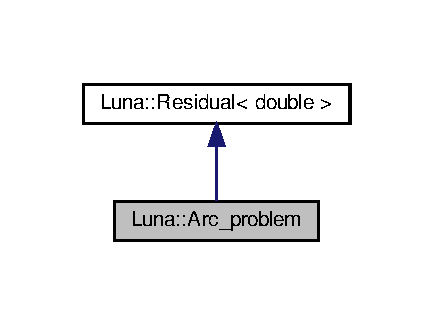
\includegraphics[width=208pt]{classLuna_1_1Arc__problem__inherit__graph}
\end{center}
\end{figure}


Collaboration diagram for Luna\+:\+:Arc\+\_\+problem\+:\nopagebreak
\begin{figure}[H]
\begin{center}
\leavevmode
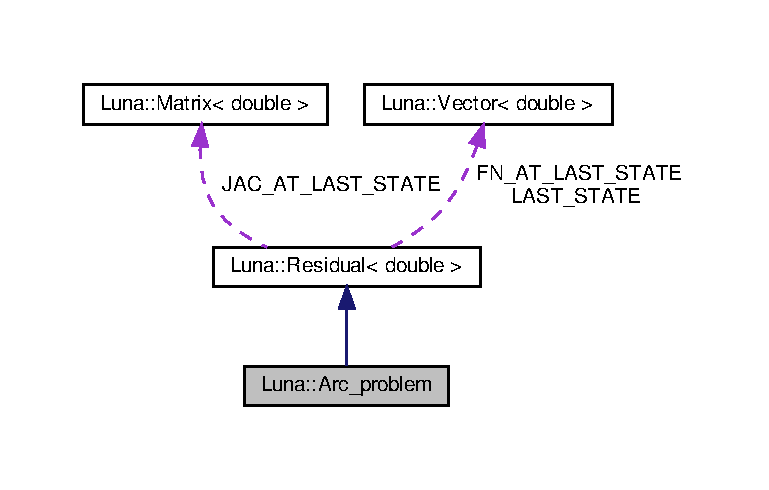
\includegraphics[width=350pt]{classLuna_1_1Arc__problem__coll__graph}
\end{center}
\end{figure}
\subsection*{Public Member Functions}
\begin{DoxyCompactItemize}
\item 
\hyperlink{classLuna_1_1Arc__problem_ac336f241d3d00f8799f038b7d2ab6c87}{Arc\+\_\+problem} ()
\item 
void \hyperlink{classLuna_1_1Arc__problem_aeb5e14b8b06d0ad0f8b42cb280836f97}{residual\+\_\+fn} (const \hyperlink{classLuna_1_1Vector}{Vector}$<$ double $>$ \&x, \hyperlink{classLuna_1_1Vector}{Vector}$<$ double $>$ \&F) const
\begin{DoxyCompactList}\small\item\em The residual function to be defined later. \end{DoxyCompactList}\end{DoxyCompactItemize}
\subsection*{Public Attributes}
\begin{DoxyCompactItemize}
\item 
double \hyperlink{classLuna_1_1Arc__problem_ab747ff77d23c83ebf8e0e8ab58e9c432}{p}
\end{DoxyCompactItemize}
\subsection*{Additional Inherited Members}


\subsection{Detailed Description}


Definition at line 33 of file Root\+\_\+finding.\+cpp.



\subsection{Constructor \& Destructor Documentation}
\mbox{\Hypertarget{classLuna_1_1Arc__problem_ac336f241d3d00f8799f038b7d2ab6c87}\label{classLuna_1_1Arc__problem_ac336f241d3d00f8799f038b7d2ab6c87}} 
\index{Luna\+::\+Arc\+\_\+problem@{Luna\+::\+Arc\+\_\+problem}!Arc\+\_\+problem@{Arc\+\_\+problem}}
\index{Arc\+\_\+problem@{Arc\+\_\+problem}!Luna\+::\+Arc\+\_\+problem@{Luna\+::\+Arc\+\_\+problem}}
\subsubsection{\texorpdfstring{Arc\+\_\+problem()}{Arc\_problem()}}
{\footnotesize\ttfamily Luna\+::\+Arc\+\_\+problem\+::\+Arc\+\_\+problem (\begin{DoxyParamCaption}{ }\end{DoxyParamCaption})\hspace{0.3cm}{\ttfamily [inline]}}



Definition at line 38 of file Root\+\_\+finding.\+cpp.


\begin{DoxyCode}
38 : \hyperlink{classLuna_1_1Residual}{Residual<double>}( 1 ) \{\}
\end{DoxyCode}


\subsection{Member Function Documentation}
\mbox{\Hypertarget{classLuna_1_1Arc__problem_aeb5e14b8b06d0ad0f8b42cb280836f97}\label{classLuna_1_1Arc__problem_aeb5e14b8b06d0ad0f8b42cb280836f97}} 
\index{Luna\+::\+Arc\+\_\+problem@{Luna\+::\+Arc\+\_\+problem}!residual\+\_\+fn@{residual\+\_\+fn}}
\index{residual\+\_\+fn@{residual\+\_\+fn}!Luna\+::\+Arc\+\_\+problem@{Luna\+::\+Arc\+\_\+problem}}
\subsubsection{\texorpdfstring{residual\+\_\+fn()}{residual\_fn()}}
{\footnotesize\ttfamily void Luna\+::\+Arc\+\_\+problem\+::residual\+\_\+fn (\begin{DoxyParamCaption}\item[{const \hyperlink{classLuna_1_1Vector}{Vector}$<$ double $>$ \&}]{state,  }\item[{\hyperlink{classLuna_1_1Vector}{Vector}$<$ double $>$ \&}]{f }\end{DoxyParamCaption}) const\hspace{0.3cm}{\ttfamily [inline]}, {\ttfamily [virtual]}}



The residual function to be defined later. 


\begin{DoxyParams}{Parameters}
{\em state} & The current state \hyperlink{classLuna_1_1Vector}{Vector} \\
\hline
{\em f} & The function \hyperlink{classLuna_1_1Vector}{Vector} to be updated \\
\hline
\end{DoxyParams}


Reimplemented from \hyperlink{classLuna_1_1Residual_ae1b1ebe3314c788b176bcac7b328de5c}{Luna\+::\+Residual$<$ double $>$}.



Definition at line 40 of file Root\+\_\+finding.\+cpp.


\begin{DoxyCode}
41       \{
42         F[ 0 ] = \hyperlink{namespaceHeat__plot_aa88370c16b85b784ccbde3ed88bc1991}{x}[ 0 ] * \hyperlink{namespaceHeat__plot_aa88370c16b85b784ccbde3ed88bc1991}{x}[ 0 ] + \hyperlink{classLuna_1_1Arc__problem_ab747ff77d23c83ebf8e0e8ab58e9c432}{p} * \hyperlink{classLuna_1_1Arc__problem_ab747ff77d23c83ebf8e0e8ab58e9c432}{p} - 2.0;
43         \textcolor{comment}{/*}
44 \textcolor{comment}{          x^2 + p^2 - 2 = 0}
45 \textcolor{comment}{        */}
46       \}
\end{DoxyCode}


\subsection{Member Data Documentation}
\mbox{\Hypertarget{classLuna_1_1Arc__problem_ab747ff77d23c83ebf8e0e8ab58e9c432}\label{classLuna_1_1Arc__problem_ab747ff77d23c83ebf8e0e8ab58e9c432}} 
\index{Luna\+::\+Arc\+\_\+problem@{Luna\+::\+Arc\+\_\+problem}!p@{p}}
\index{p@{p}!Luna\+::\+Arc\+\_\+problem@{Luna\+::\+Arc\+\_\+problem}}
\subsubsection{\texorpdfstring{p}{p}}
{\footnotesize\ttfamily double Luna\+::\+Arc\+\_\+problem\+::p}



Definition at line 36 of file Root\+\_\+finding.\+cpp.



Referenced by main().



The documentation for this class was generated from the following file\+:\begin{DoxyCompactItemize}
\item 
Examples/\hyperlink{Root__finding_8cpp}{Root\+\_\+finding.\+cpp}\end{DoxyCompactItemize}

\hypertarget{classLuna_1_1Arclength}{}\section{Luna\+:\+:Arclength$<$ T $>$ Class Template Reference}
\label{classLuna_1_1Arclength}\index{Luna\+::\+Arclength$<$ T $>$@{Luna\+::\+Arclength$<$ T $>$}}


A templated arc length solver class.  




{\ttfamily \#include $<$Arclength.\+h$>$}



Inheritance diagram for Luna\+:\+:Arclength$<$ T $>$\+:\nopagebreak
\begin{figure}[H]
\begin{center}
\leavevmode
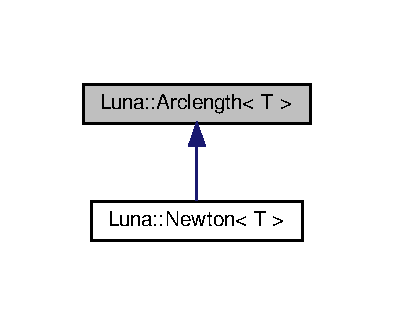
\includegraphics[width=189pt]{classLuna_1_1Arclength__inherit__graph}
\end{center}
\end{figure}


Collaboration diagram for Luna\+:\+:Arclength$<$ T $>$\+:\nopagebreak
\begin{figure}[H]
\begin{center}
\leavevmode
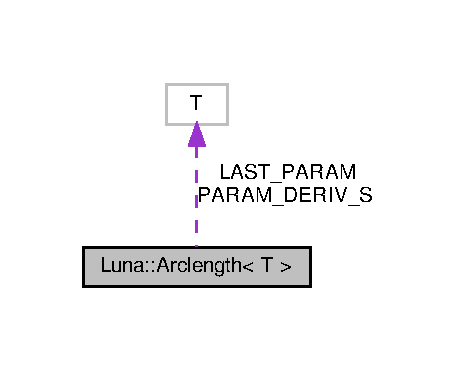
\includegraphics[width=220pt]{classLuna_1_1Arclength__coll__graph}
\end{center}
\end{figure}
\subsection*{Public Member Functions}
\begin{DoxyCompactItemize}
\item 
\hyperlink{classLuna_1_1Arclength_afa2eac838a1005897d0f82815764237f}{Arclength} ()
\begin{DoxyCompactList}\small\item\em Constructor. \end{DoxyCompactList}\item 
virtual \hyperlink{classLuna_1_1Arclength_acd49e172150ec06785b68bf84a9e818e}{$\sim$\+Arclength} ()
\begin{DoxyCompactList}\small\item\em Destructor. \end{DoxyCompactList}\item 
void \hyperlink{classLuna_1_1Arclength_a37c85555280cd6fbcf4acc72c92c5f41}{init\+\_\+arc} (\hyperlink{classLuna_1_1Vector}{Vector}$<$ T $>$ x, T $\ast$ptr\+\_\+param, const double \&\hyperlink{classLuna_1_1Arclength_af92962a44295884704ebc6196ffbd6f6}{ds}, const double \&max\+\_\+ds)
\begin{DoxyCompactList}\small\item\em Initialise the arc-\/length continuation class. \end{DoxyCompactList}\item 
virtual void \hyperlink{classLuna_1_1Arclength_a0829d51bb49011f5ed56c25b7554d115}{solve} (\hyperlink{classLuna_1_1Vector}{Vector}$<$ T $>$ \&x)=0
\begin{DoxyCompactList}\small\item\em Solve the system for a given initial guess. \end{DoxyCompactList}\item 
double \& \hyperlink{classLuna_1_1Arclength_af92962a44295884704ebc6196ffbd6f6}{ds} ()
\begin{DoxyCompactList}\small\item\em A handle to the arc-\/length step. \end{DoxyCompactList}\item 
double \& \hyperlink{classLuna_1_1Arclength_a2c080f19e24df1cd4e146bd79a88b6c7}{arcstep\+\_\+multiplier} ()
\begin{DoxyCompactList}\small\item\em A handle to the arc step multiplier. \end{DoxyCompactList}\item 
bool \& \hyperlink{classLuna_1_1Arclength_ad7be910825086e7faa134bf956342a82}{rescale\+\_\+theta} ()
\begin{DoxyCompactList}\small\item\em A handle to the R\+E\+S\+C\+A\+L\+E\+\_\+\+T\+H\+E\+TA flag. \end{DoxyCompactList}\item 
double \& \hyperlink{classLuna_1_1Arclength_a7e117fb2774052fc240e0eb0e4aac08c}{theta} ()
\begin{DoxyCompactList}\small\item\em A handle to the theta parameter. \end{DoxyCompactList}\item 
double \& \hyperlink{classLuna_1_1Arclength_a4a14037ceffcca21d1417c22894470fb}{desired\+\_\+arc\+\_\+proportion} ()
\begin{DoxyCompactList}\small\item\em A handle to the desired proportion of the parameter to be used. \end{DoxyCompactList}\end{DoxyCompactItemize}
\subsection*{Protected Member Functions}
\begin{DoxyCompactItemize}
\item 
void \hyperlink{classLuna_1_1Arclength_a8941ac2150d8a53aaefbf5825553c86b}{update} (const \hyperlink{classLuna_1_1Vector}{Vector}$<$ T $>$ \&x)
\begin{DoxyCompactList}\small\item\em Store the current converged state and parameter \& compute derivatives. \end{DoxyCompactList}\item 
double \hyperlink{classLuna_1_1Arclength_af47a50bb4ce666b505fe990ab44063db}{arclength\+\_\+residual} (const \hyperlink{classLuna_1_1Vector}{Vector}$<$ T $>$ \&x) const
\begin{DoxyCompactList}\small\item\em Extra constraint that is to be used to replace the unknown arc-\/length. \end{DoxyCompactList}\item 
\hyperlink{classLuna_1_1Vector}{Vector}$<$ T $>$ \hyperlink{classLuna_1_1Arclength_a3bffa2fa38c73cd97155289bc902ccc6}{Jac\+\_\+arclength\+\_\+residual} (\hyperlink{classLuna_1_1Vector}{Vector}$<$ T $>$ \&x) const
\begin{DoxyCompactList}\small\item\em Return the derivative of the arclength\+\_\+residual function. \end{DoxyCompactList}\item 
void \hyperlink{classLuna_1_1Arclength_a47d02a96d4b0a5112e6b06d3787409b5}{update\+\_\+theta} (const \hyperlink{classLuna_1_1Vector}{Vector}$<$ T $>$ \&x)
\begin{DoxyCompactList}\small\item\em Automatically update theta value only if R\+E\+S\+C\+A\+L\+E\+\_\+\+T\+H\+E\+TA = true. \end{DoxyCompactList}\end{DoxyCompactItemize}
\subsection*{Protected Attributes}
\begin{DoxyCompactItemize}
\item 
T $\ast$ \hyperlink{classLuna_1_1Arclength_a984cead721a38abf1ab2a489052461e0}{ptr\+\_\+\+P\+A\+R\+AM}
\item 
\hyperlink{classLuna_1_1Vector}{Vector}$<$ T $>$ \hyperlink{classLuna_1_1Arclength_a6d6ba83245b4dd616d265609a93035a2}{L\+A\+S\+T\+\_\+X}
\item 
\hyperlink{classLuna_1_1Vector}{Vector}$<$ T $>$ \hyperlink{classLuna_1_1Arclength_a0108e51178f63927883af0b0022c29ad}{X\+\_\+\+D\+E\+R\+I\+V\+\_\+S}
\item 
T \hyperlink{classLuna_1_1Arclength_a98e8241f24a16ea9f12e514d8d8f841b}{L\+A\+S\+T\+\_\+\+P\+A\+R\+AM}
\item 
T \hyperlink{classLuna_1_1Arclength_a5a02856595774b4a96e4d8add5d9baa4}{P\+A\+R\+A\+M\+\_\+\+D\+E\+R\+I\+V\+\_\+S}
\item 
double \hyperlink{classLuna_1_1Arclength_a6797d7b76d3e27c00b9c4c6ab9970405}{DS}
\item 
double \hyperlink{classLuna_1_1Arclength_a8fcd2b977d7ce78342f113d4e69ad8f1}{M\+A\+X\+\_\+\+DS}
\item 
double \hyperlink{classLuna_1_1Arclength_ae1ff8d41d3e81d9ce335d19de4a269cc}{A\+R\+C\+S\+T\+E\+P\+\_\+\+M\+U\+L\+T\+I\+P\+L\+I\+ER}
\item 
bool \hyperlink{classLuna_1_1Arclength_a9bf5e636e7a0772f3ba5476ec2c83f6a}{I\+N\+I\+T\+I\+A\+L\+I\+S\+ED}
\item 
double \hyperlink{classLuna_1_1Arclength_aa17766cf4bcbe5b063dc2a95f89baf42}{T\+H\+E\+TA}
\end{DoxyCompactItemize}


\subsection{Detailed Description}
\subsubsection*{template$<$class T$>$\newline
class Luna\+::\+Arclength$<$ T $>$}

A templated arc length solver class. 

Definition at line 17 of file Arclength.\+h.



\subsection{Constructor \& Destructor Documentation}
\mbox{\Hypertarget{classLuna_1_1Arclength_afa2eac838a1005897d0f82815764237f}\label{classLuna_1_1Arclength_afa2eac838a1005897d0f82815764237f}} 
\index{Luna\+::\+Arclength@{Luna\+::\+Arclength}!Arclength@{Arclength}}
\index{Arclength@{Arclength}!Luna\+::\+Arclength@{Luna\+::\+Arclength}}
\subsubsection{\texorpdfstring{Arclength()}{Arclength()}}
{\footnotesize\ttfamily template$<$class T $>$ \\
\hyperlink{classLuna_1_1Arclength}{Luna\+::\+Arclength}$<$ T $>$\+::\hyperlink{classLuna_1_1Arclength}{Arclength} (\begin{DoxyParamCaption}{ }\end{DoxyParamCaption})\hspace{0.3cm}{\ttfamily [inline]}}



Constructor. 



Definition at line 58 of file Arclength.\+h.


\begin{DoxyCode}
58                   : \hyperlink{classLuna_1_1Arclength_ae1ff8d41d3e81d9ce335d19de4a269cc}{ARCSTEP\_MULTIPLIER}( 2.0 ),
59                     \hyperlink{classLuna_1_1Arclength_a9bf5e636e7a0772f3ba5476ec2c83f6a}{INITIALISED}( \textcolor{keyword}{false} ),
60                     \hyperlink{classLuna_1_1Arclength_aa17766cf4bcbe5b063dc2a95f89baf42}{THETA}( 0.5 ),
61                     DESIRED\_ARC\_PROPORTION( 0.5 ),
62                     RESCALE\_THETA( \textcolor{keyword}{false} )
63       \{\}
\end{DoxyCode}
\mbox{\Hypertarget{classLuna_1_1Arclength_acd49e172150ec06785b68bf84a9e818e}\label{classLuna_1_1Arclength_acd49e172150ec06785b68bf84a9e818e}} 
\index{Luna\+::\+Arclength@{Luna\+::\+Arclength}!````~Arclength@{$\sim$\+Arclength}}
\index{````~Arclength@{$\sim$\+Arclength}!Luna\+::\+Arclength@{Luna\+::\+Arclength}}
\subsubsection{\texorpdfstring{$\sim$\+Arclength()}{~Arclength()}}
{\footnotesize\ttfamily template$<$class T $>$ \\
virtual \hyperlink{classLuna_1_1Arclength}{Luna\+::\+Arclength}$<$ T $>$\+::$\sim$\hyperlink{classLuna_1_1Arclength}{Arclength} (\begin{DoxyParamCaption}{ }\end{DoxyParamCaption})\hspace{0.3cm}{\ttfamily [inline]}, {\ttfamily [virtual]}}



Destructor. 



Definition at line 66 of file Arclength.\+h.



References Luna\+::\+Arclength$<$ T $>$\+::ds(), Luna\+::\+Arclength$<$ T $>$\+::init\+\_\+arc(), Luna\+::\+Arclength$<$ T $>$\+::solve(), and Heat\+\_\+plot\+::x.


\begin{DoxyCode}
66 \{\}
\end{DoxyCode}


\subsection{Member Function Documentation}
\mbox{\Hypertarget{classLuna_1_1Arclength_af47a50bb4ce666b505fe990ab44063db}\label{classLuna_1_1Arclength_af47a50bb4ce666b505fe990ab44063db}} 
\index{Luna\+::\+Arclength@{Luna\+::\+Arclength}!arclength\+\_\+residual@{arclength\+\_\+residual}}
\index{arclength\+\_\+residual@{arclength\+\_\+residual}!Luna\+::\+Arclength@{Luna\+::\+Arclength}}
\subsubsection{\texorpdfstring{arclength\+\_\+residual()}{arclength\_residual()}}
{\footnotesize\ttfamily template$<$typename T $>$ \\
double \hyperlink{classLuna_1_1Arclength}{Luna\+::\+Arclength}$<$ T $>$\+::arclength\+\_\+residual (\begin{DoxyParamCaption}\item[{const \hyperlink{classLuna_1_1Vector}{Vector}$<$ T $>$ \&}]{x }\end{DoxyParamCaption}) const\hspace{0.3cm}{\ttfamily [protected]}}



Extra constraint that is to be used to replace the unknown arc-\/length. 


\begin{DoxyParams}{Parameters}
{\em x} & The current state \hyperlink{classLuna_1_1Vector}{Vector} \\
\hline
\end{DoxyParams}


Definition at line 115 of file Arclength.\+h.



References Luna\+::\+Arclength$<$ T $>$\+::\+DS, Luna\+::\+Arclength$<$ T $>$\+::\+L\+A\+S\+T\+\_\+\+P\+A\+R\+AM, Luna\+::\+Arclength$<$ T $>$\+::\+L\+A\+S\+T\+\_\+X, Luna\+::\+Arclength$<$ T $>$\+::ptr\+\_\+\+P\+A\+R\+AM, Luna\+::\+Vector$<$ T $>$\+::size(), and Luna\+::\+Arclength$<$ T $>$\+::\+T\+H\+E\+TA.



Referenced by Luna\+::\+Newton$<$ T $>$\+::arclength\+\_\+solve().


\begin{DoxyCode}
116   \{
117     \textcolor{keywordflow}{return} \hyperlink{classLuna_1_1Arclength_aa17766cf4bcbe5b063dc2a95f89baf42}{THETA} * ( \hyperlink{namespaceHeat__plot_aa88370c16b85b784ccbde3ed88bc1991}{x} - \hyperlink{classLuna_1_1Arclength_a6d6ba83245b4dd616d265609a93035a2}{LAST\_X} ).norm\_2() / \hyperlink{namespaceHeat__plot_aa88370c16b85b784ccbde3ed88bc1991}{x}.size() + ( 1.0 - 
      \hyperlink{classLuna_1_1Arclength_aa17766cf4bcbe5b063dc2a95f89baf42}{THETA} )
118                * std::pow( std::abs( *\hyperlink{classLuna_1_1Arclength_a984cead721a38abf1ab2a489052461e0}{ptr\_PARAM} - \hyperlink{classLuna_1_1Arclength_a98e8241f24a16ea9f12e514d8d8f841b}{LAST\_PARAM} ), 2 ) - 
      \hyperlink{classLuna_1_1Arclength_a6797d7b76d3e27c00b9c4c6ab9970405}{DS} * \hyperlink{classLuna_1_1Arclength_a6797d7b76d3e27c00b9c4c6ab9970405}{DS};
119   \}
\end{DoxyCode}
\mbox{\Hypertarget{classLuna_1_1Arclength_a2c080f19e24df1cd4e146bd79a88b6c7}\label{classLuna_1_1Arclength_a2c080f19e24df1cd4e146bd79a88b6c7}} 
\index{Luna\+::\+Arclength@{Luna\+::\+Arclength}!arcstep\+\_\+multiplier@{arcstep\+\_\+multiplier}}
\index{arcstep\+\_\+multiplier@{arcstep\+\_\+multiplier}!Luna\+::\+Arclength@{Luna\+::\+Arclength}}
\subsubsection{\texorpdfstring{arcstep\+\_\+multiplier()}{arcstep\_multiplier()}}
{\footnotesize\ttfamily template$<$class T $>$ \\
double\& \hyperlink{classLuna_1_1Arclength}{Luna\+::\+Arclength}$<$ T $>$\+::arcstep\+\_\+multiplier (\begin{DoxyParamCaption}{ }\end{DoxyParamCaption})\hspace{0.3cm}{\ttfamily [inline]}}



A handle to the arc step multiplier. 

\begin{DoxyReturn}{Returns}
The arc-\/length step multiplier 
\end{DoxyReturn}


Definition at line 88 of file Arclength.\+h.



References Luna\+::\+Arclength$<$ T $>$\+::\+A\+R\+C\+S\+T\+E\+P\+\_\+\+M\+U\+L\+T\+I\+P\+L\+I\+ER.


\begin{DoxyCode}
88 \{ \textcolor{keywordflow}{return} \hyperlink{classLuna_1_1Arclength_ae1ff8d41d3e81d9ce335d19de4a269cc}{ARCSTEP\_MULTIPLIER}; \}
\end{DoxyCode}
\mbox{\Hypertarget{classLuna_1_1Arclength_a4a14037ceffcca21d1417c22894470fb}\label{classLuna_1_1Arclength_a4a14037ceffcca21d1417c22894470fb}} 
\index{Luna\+::\+Arclength@{Luna\+::\+Arclength}!desired\+\_\+arc\+\_\+proportion@{desired\+\_\+arc\+\_\+proportion}}
\index{desired\+\_\+arc\+\_\+proportion@{desired\+\_\+arc\+\_\+proportion}!Luna\+::\+Arclength@{Luna\+::\+Arclength}}
\subsubsection{\texorpdfstring{desired\+\_\+arc\+\_\+proportion()}{desired\_arc\_proportion()}}
{\footnotesize\ttfamily template$<$class T $>$ \\
double\& \hyperlink{classLuna_1_1Arclength}{Luna\+::\+Arclength}$<$ T $>$\+::desired\+\_\+arc\+\_\+proportion (\begin{DoxyParamCaption}{ }\end{DoxyParamCaption})\hspace{0.3cm}{\ttfamily [inline]}}



A handle to the desired proportion of the parameter to be used. 

\begin{DoxyReturn}{Returns}
The desired proportion of the arc-\/length 
\end{DoxyReturn}


Definition at line 100 of file Arclength.\+h.


\begin{DoxyCode}
100 \{ \textcolor{keywordflow}{return} DESIRED\_ARC\_PROPORTION; \}
\end{DoxyCode}
\mbox{\Hypertarget{classLuna_1_1Arclength_af92962a44295884704ebc6196ffbd6f6}\label{classLuna_1_1Arclength_af92962a44295884704ebc6196ffbd6f6}} 
\index{Luna\+::\+Arclength@{Luna\+::\+Arclength}!ds@{ds}}
\index{ds@{ds}!Luna\+::\+Arclength@{Luna\+::\+Arclength}}
\subsubsection{\texorpdfstring{ds()}{ds()}}
{\footnotesize\ttfamily template$<$class T $>$ \\
double\& \hyperlink{classLuna_1_1Arclength}{Luna\+::\+Arclength}$<$ T $>$\+::ds (\begin{DoxyParamCaption}{ }\end{DoxyParamCaption})\hspace{0.3cm}{\ttfamily [inline]}}



A handle to the arc-\/length step. 

\begin{DoxyReturn}{Returns}
The arc-\/length step 
\end{DoxyReturn}


Definition at line 84 of file Arclength.\+h.



References Luna\+::\+Arclength$<$ T $>$\+::\+DS.



Referenced by Luna\+::\+Arclength$<$ T $>$\+::init\+\_\+arc(), and Luna\+::\+Arclength$<$ T $>$\+::$\sim$\+Arclength().


\begin{DoxyCode}
84 \{ \textcolor{keywordflow}{return} \hyperlink{classLuna_1_1Arclength_a6797d7b76d3e27c00b9c4c6ab9970405}{DS}; \}
\end{DoxyCode}
\mbox{\Hypertarget{classLuna_1_1Arclength_a37c85555280cd6fbcf4acc72c92c5f41}\label{classLuna_1_1Arclength_a37c85555280cd6fbcf4acc72c92c5f41}} 
\index{Luna\+::\+Arclength@{Luna\+::\+Arclength}!init\+\_\+arc@{init\+\_\+arc}}
\index{init\+\_\+arc@{init\+\_\+arc}!Luna\+::\+Arclength@{Luna\+::\+Arclength}}
\subsubsection{\texorpdfstring{init\+\_\+arc()}{init\_arc()}}
{\footnotesize\ttfamily template$<$class T $>$ \\
void \hyperlink{classLuna_1_1Arclength}{Luna\+::\+Arclength}$<$ T $>$\+::init\+\_\+arc (\begin{DoxyParamCaption}\item[{\hyperlink{classLuna_1_1Vector}{Vector}$<$ T $>$}]{x,  }\item[{T $\ast$}]{ptr\+\_\+param,  }\item[{const double \&}]{ds,  }\item[{const double \&}]{max\+\_\+ds }\end{DoxyParamCaption})}



Initialise the arc-\/length continuation class. 


\begin{DoxyParams}{Parameters}
{\em x} & The current state \hyperlink{classLuna_1_1Vector}{Vector} \\
\hline
{\em ptr\+\_\+param} & Pointer to the arc-\/length parameter \\
\hline
{\em ds} & The size of the arc-\/length step \\
\hline
{\em max\+\_\+ds} & The maximum arc-\/length step to be taken \\
\hline
\end{DoxyParams}


Definition at line 143 of file Arclength.\+h.



References Luna\+::\+Arclength$<$ T $>$\+::\+DS, Luna\+::\+Arclength$<$ T $>$\+::ds(), Luna\+::\+Arclength$<$ T $>$\+::\+I\+N\+I\+T\+I\+A\+L\+I\+S\+ED, Luna\+::\+Arclength$<$ T $>$\+::\+L\+A\+S\+T\+\_\+\+P\+A\+R\+AM, Luna\+::\+Arclength$<$ T $>$\+::\+L\+A\+S\+T\+\_\+X, Luna\+::\+Arclength$<$ T $>$\+::\+M\+A\+X\+\_\+\+DS, Luna\+::\+Arclength$<$ T $>$\+::ptr\+\_\+\+P\+A\+R\+AM, Luna\+::\+Arclength$<$ T $>$\+::solve(), Luna\+::\+Arclength$<$ T $>$\+::update(), and Heat\+\_\+plot\+::x.



Referenced by main(), and Luna\+::\+Arclength$<$ T $>$\+::$\sim$\+Arclength().


\begin{DoxyCode}
145   \{
146     \hyperlink{classLuna_1_1Arclength_a984cead721a38abf1ab2a489052461e0}{ptr\_PARAM} = ptr\_param;
147     \hyperlink{classLuna_1_1Arclength_a0829d51bb49011f5ed56c25b7554d115}{solve}( \hyperlink{namespaceHeat__plot_aa88370c16b85b784ccbde3ed88bc1991}{x} );
148     \hyperlink{classLuna_1_1Arclength_a6d6ba83245b4dd616d265609a93035a2}{LAST\_X} = \hyperlink{namespaceHeat__plot_aa88370c16b85b784ccbde3ed88bc1991}{x};
149     \hyperlink{classLuna_1_1Arclength_a98e8241f24a16ea9f12e514d8d8f841b}{LAST\_PARAM} = *\hyperlink{classLuna_1_1Arclength_a984cead721a38abf1ab2a489052461e0}{ptr\_PARAM};
150     \textcolor{comment}{// We now have one solution which we can use to arc-length continue}
151     \hyperlink{classLuna_1_1Arclength_a6797d7b76d3e27c00b9c4c6ab9970405}{DS} = \hyperlink{classLuna_1_1Arclength_af92962a44295884704ebc6196ffbd6f6}{ds};
152     *\hyperlink{classLuna_1_1Arclength_a984cead721a38abf1ab2a489052461e0}{ptr\_PARAM} += \hyperlink{classLuna_1_1Arclength_a6797d7b76d3e27c00b9c4c6ab9970405}{DS};
153     \textcolor{comment}{// Recompute the state at this new parameter value}
154     \hyperlink{classLuna_1_1Arclength_a0829d51bb49011f5ed56c25b7554d115}{solve}( \hyperlink{namespaceHeat__plot_aa88370c16b85b784ccbde3ed88bc1991}{x} );
155     \hyperlink{classLuna_1_1Arclength_a8941ac2150d8a53aaefbf5825553c86b}{update}( \hyperlink{namespaceHeat__plot_aa88370c16b85b784ccbde3ed88bc1991}{x} );
156     \hyperlink{classLuna_1_1Arclength_a9bf5e636e7a0772f3ba5476ec2c83f6a}{INITIALISED} = \textcolor{keyword}{true};
157     \hyperlink{classLuna_1_1Arclength_a8fcd2b977d7ce78342f113d4e69ad8f1}{MAX\_DS} = max\_ds;
158   \}
\end{DoxyCode}
\mbox{\Hypertarget{classLuna_1_1Arclength_a3bffa2fa38c73cd97155289bc902ccc6}\label{classLuna_1_1Arclength_a3bffa2fa38c73cd97155289bc902ccc6}} 
\index{Luna\+::\+Arclength@{Luna\+::\+Arclength}!Jac\+\_\+arclength\+\_\+residual@{Jac\+\_\+arclength\+\_\+residual}}
\index{Jac\+\_\+arclength\+\_\+residual@{Jac\+\_\+arclength\+\_\+residual}!Luna\+::\+Arclength@{Luna\+::\+Arclength}}
\subsubsection{\texorpdfstring{Jac\+\_\+arclength\+\_\+residual()}{Jac\_arclength\_residual()}}
{\footnotesize\ttfamily template$<$typename T $>$ \\
\hyperlink{classLuna_1_1Vector}{Vector}$<$ T $>$ \hyperlink{classLuna_1_1Arclength}{Luna\+::\+Arclength}$<$ T $>$\+::Jac\+\_\+arclength\+\_\+residual (\begin{DoxyParamCaption}\item[{\hyperlink{classLuna_1_1Vector}{Vector}$<$ T $>$ \&}]{x }\end{DoxyParamCaption}) const\hspace{0.3cm}{\ttfamily [protected]}}



Return the derivative of the arclength\+\_\+residual function. 

with respect to each state variable 
\begin{DoxyParams}{Parameters}
{\em x} & The current state \hyperlink{classLuna_1_1Vector}{Vector} \\
\hline
\end{DoxyParams}
\begin{DoxyReturn}{Returns}
The derivative of the arclength\+\_\+residual function 
\end{DoxyReturn}


Definition at line 122 of file Arclength.\+h.



References Luna\+::\+Arclength$<$ T $>$\+::\+L\+A\+S\+T\+\_\+X, Luna\+::\+Vector$<$ T $>$\+::size(), and Luna\+::\+Arclength$<$ T $>$\+::\+T\+H\+E\+TA.



Referenced by Luna\+::\+Newton$<$ T $>$\+::arclength\+\_\+solve().


\begin{DoxyCode}
123     \{
124         Vector<T> Jx( \hyperlink{namespaceHeat__plot_aa88370c16b85b784ccbde3ed88bc1991}{x} - \hyperlink{classLuna_1_1Arclength_a6d6ba83245b4dd616d265609a93035a2}{LAST\_X} );
125         Jx = Jx * ( \hyperlink{classLuna_1_1Arclength_aa17766cf4bcbe5b063dc2a95f89baf42}{THETA} / ( \hyperlink{namespaceHeat__plot_aa88370c16b85b784ccbde3ed88bc1991}{x}.size() * ( \hyperlink{namespaceHeat__plot_aa88370c16b85b784ccbde3ed88bc1991}{x} - \hyperlink{classLuna_1_1Arclength_a6d6ba83245b4dd616d265609a93035a2}{LAST\_X} ).norm\_2() ) );
126         \textcolor{keywordflow}{return} Jx;
127     \}
\end{DoxyCode}
\mbox{\Hypertarget{classLuna_1_1Arclength_ad7be910825086e7faa134bf956342a82}\label{classLuna_1_1Arclength_ad7be910825086e7faa134bf956342a82}} 
\index{Luna\+::\+Arclength@{Luna\+::\+Arclength}!rescale\+\_\+theta@{rescale\+\_\+theta}}
\index{rescale\+\_\+theta@{rescale\+\_\+theta}!Luna\+::\+Arclength@{Luna\+::\+Arclength}}
\subsubsection{\texorpdfstring{rescale\+\_\+theta()}{rescale\_theta()}}
{\footnotesize\ttfamily template$<$class T $>$ \\
bool\& \hyperlink{classLuna_1_1Arclength}{Luna\+::\+Arclength}$<$ T $>$\+::rescale\+\_\+theta (\begin{DoxyParamCaption}{ }\end{DoxyParamCaption})\hspace{0.3cm}{\ttfamily [inline]}}



A handle to the R\+E\+S\+C\+A\+L\+E\+\_\+\+T\+H\+E\+TA flag. 

\begin{DoxyReturn}{Returns}
The theta rescale flag 
\end{DoxyReturn}


Definition at line 92 of file Arclength.\+h.


\begin{DoxyCode}
92 \{ \textcolor{keywordflow}{return} RESCALE\_THETA; \}
\end{DoxyCode}
\mbox{\Hypertarget{classLuna_1_1Arclength_a0829d51bb49011f5ed56c25b7554d115}\label{classLuna_1_1Arclength_a0829d51bb49011f5ed56c25b7554d115}} 
\index{Luna\+::\+Arclength@{Luna\+::\+Arclength}!solve@{solve}}
\index{solve@{solve}!Luna\+::\+Arclength@{Luna\+::\+Arclength}}
\subsubsection{\texorpdfstring{solve()}{solve()}}
{\footnotesize\ttfamily template$<$class T $>$ \\
void \hyperlink{classLuna_1_1Arclength}{Luna\+::\+Arclength}$<$ T $>$\+::solve (\begin{DoxyParamCaption}\item[{\hyperlink{classLuna_1_1Vector}{Vector}$<$ T $>$ \&}]{x }\end{DoxyParamCaption})\hspace{0.3cm}{\ttfamily [pure virtual]}}



Solve the system for a given initial guess. 


\begin{DoxyParams}{Parameters}
{\em x} & The current state \hyperlink{classLuna_1_1Vector}{Vector} \\
\hline
\end{DoxyParams}


Implemented in \hyperlink{classLuna_1_1Newton_a1d5ebdbfd8910c40ed58244f6348b13e}{Luna\+::\+Newton$<$ T $>$}.



Definition at line 161 of file Arclength.\+h.



Referenced by Luna\+::\+Arclength$<$ T $>$\+::init\+\_\+arc(), and Luna\+::\+Arclength$<$ T $>$\+::$\sim$\+Arclength().


\begin{DoxyCode}
161 \{\}
\end{DoxyCode}
\mbox{\Hypertarget{classLuna_1_1Arclength_a7e117fb2774052fc240e0eb0e4aac08c}\label{classLuna_1_1Arclength_a7e117fb2774052fc240e0eb0e4aac08c}} 
\index{Luna\+::\+Arclength@{Luna\+::\+Arclength}!theta@{theta}}
\index{theta@{theta}!Luna\+::\+Arclength@{Luna\+::\+Arclength}}
\subsubsection{\texorpdfstring{theta()}{theta()}}
{\footnotesize\ttfamily template$<$class T $>$ \\
double\& \hyperlink{classLuna_1_1Arclength}{Luna\+::\+Arclength}$<$ T $>$\+::theta (\begin{DoxyParamCaption}{ }\end{DoxyParamCaption})\hspace{0.3cm}{\ttfamily [inline]}}



A handle to the theta parameter. 

\begin{DoxyReturn}{Returns}
The Theta weighting parameter 
\end{DoxyReturn}


Definition at line 96 of file Arclength.\+h.



References Luna\+::\+Arclength$<$ T $>$\+::\+T\+H\+E\+TA.


\begin{DoxyCode}
96 \{ \textcolor{keywordflow}{return} \hyperlink{classLuna_1_1Arclength_aa17766cf4bcbe5b063dc2a95f89baf42}{THETA}; \}
\end{DoxyCode}
\mbox{\Hypertarget{classLuna_1_1Arclength_a8941ac2150d8a53aaefbf5825553c86b}\label{classLuna_1_1Arclength_a8941ac2150d8a53aaefbf5825553c86b}} 
\index{Luna\+::\+Arclength@{Luna\+::\+Arclength}!update@{update}}
\index{update@{update}!Luna\+::\+Arclength@{Luna\+::\+Arclength}}
\subsubsection{\texorpdfstring{update()}{update()}}
{\footnotesize\ttfamily template$<$typename T $>$ \\
void \hyperlink{classLuna_1_1Arclength}{Luna\+::\+Arclength}$<$ T $>$\+::update (\begin{DoxyParamCaption}\item[{const \hyperlink{classLuna_1_1Vector}{Vector}$<$ T $>$ \&}]{x }\end{DoxyParamCaption})\hspace{0.3cm}{\ttfamily [protected]}}



Store the current converged state and parameter \& compute derivatives. 


\begin{DoxyParams}{Parameters}
{\em x} & The current state \hyperlink{classLuna_1_1Vector}{Vector} \\
\hline
\end{DoxyParams}


Definition at line 105 of file Arclength.\+h.



References Luna\+::\+Arclength$<$ T $>$\+::\+DS, Luna\+::\+Arclength$<$ T $>$\+::\+L\+A\+S\+T\+\_\+\+P\+A\+R\+AM, Luna\+::\+Arclength$<$ T $>$\+::\+L\+A\+S\+T\+\_\+X, Luna\+::\+Arclength$<$ T $>$\+::\+P\+A\+R\+A\+M\+\_\+\+D\+E\+R\+I\+V\+\_\+S, Luna\+::\+Arclength$<$ T $>$\+::ptr\+\_\+\+P\+A\+R\+AM, Luna\+::\+Arclength$<$ T $>$\+::update\+\_\+theta(), Heat\+\_\+plot\+::x, and Luna\+::\+Arclength$<$ T $>$\+::\+X\+\_\+\+D\+E\+R\+I\+V\+\_\+S.



Referenced by Luna\+::\+Newton$<$ T $>$\+::arclength\+\_\+solve(), Luna\+::\+Arclength$<$ T $>$\+::init\+\_\+arc(), and Luna\+::\+Newton$<$ T $>$\+::iterate().


\begin{DoxyCode}
106   \{
107     \textcolor{keywordflow}{if} ( RESCALE\_THETA ) \{ \hyperlink{classLuna_1_1Arclength_a47d02a96d4b0a5112e6b06d3787409b5}{update\_theta}( \hyperlink{namespaceHeat__plot_aa88370c16b85b784ccbde3ed88bc1991}{x} ); \}
108     \hyperlink{classLuna_1_1Arclength_a0108e51178f63927883af0b0022c29ad}{X\_DERIV\_S} = ( \hyperlink{namespaceHeat__plot_aa88370c16b85b784ccbde3ed88bc1991}{x} - \hyperlink{classLuna_1_1Arclength_a6d6ba83245b4dd616d265609a93035a2}{LAST\_X} ) / \hyperlink{classLuna_1_1Arclength_a6797d7b76d3e27c00b9c4c6ab9970405}{DS};
109     \hyperlink{classLuna_1_1Arclength_a5a02856595774b4a96e4d8add5d9baa4}{PARAM\_DERIV\_S} = ( *\hyperlink{classLuna_1_1Arclength_a984cead721a38abf1ab2a489052461e0}{ptr\_PARAM} - \hyperlink{classLuna_1_1Arclength_a98e8241f24a16ea9f12e514d8d8f841b}{LAST\_PARAM} ) / 
      \hyperlink{classLuna_1_1Arclength_a6797d7b76d3e27c00b9c4c6ab9970405}{DS};
110     \hyperlink{classLuna_1_1Arclength_a6d6ba83245b4dd616d265609a93035a2}{LAST\_X} = \hyperlink{namespaceHeat__plot_aa88370c16b85b784ccbde3ed88bc1991}{x};
111     \hyperlink{classLuna_1_1Arclength_a98e8241f24a16ea9f12e514d8d8f841b}{LAST\_PARAM} = *\hyperlink{classLuna_1_1Arclength_a984cead721a38abf1ab2a489052461e0}{ptr\_PARAM};
112   \}
\end{DoxyCode}
\mbox{\Hypertarget{classLuna_1_1Arclength_a47d02a96d4b0a5112e6b06d3787409b5}\label{classLuna_1_1Arclength_a47d02a96d4b0a5112e6b06d3787409b5}} 
\index{Luna\+::\+Arclength@{Luna\+::\+Arclength}!update\+\_\+theta@{update\+\_\+theta}}
\index{update\+\_\+theta@{update\+\_\+theta}!Luna\+::\+Arclength@{Luna\+::\+Arclength}}
\subsubsection{\texorpdfstring{update\+\_\+theta()}{update\_theta()}}
{\footnotesize\ttfamily template$<$class T $>$ \\
void \hyperlink{classLuna_1_1Arclength}{Luna\+::\+Arclength}$<$ T $>$\+::update\+\_\+theta (\begin{DoxyParamCaption}\item[{const \hyperlink{classLuna_1_1Vector}{Vector}$<$ T $>$ \&}]{x }\end{DoxyParamCaption})\hspace{0.3cm}{\ttfamily [protected]}}



Automatically update theta value only if R\+E\+S\+C\+A\+L\+E\+\_\+\+T\+H\+E\+TA = true. 


\begin{DoxyParams}{Parameters}
{\em x} & The current state \hyperlink{classLuna_1_1Vector}{Vector} \\
\hline
\end{DoxyParams}


Definition at line 130 of file Arclength.\+h.



References Luna\+::\+Arclength$<$ T $>$\+::\+L\+A\+S\+T\+\_\+\+P\+A\+R\+AM, Luna\+::\+Arclength$<$ T $>$\+::\+L\+A\+S\+T\+\_\+X, Luna\+::\+Arclength$<$ T $>$\+::ptr\+\_\+\+P\+A\+R\+AM, Luna\+::\+Vector$<$ T $>$\+::size(), and Luna\+::\+Arclength$<$ T $>$\+::\+T\+H\+E\+TA.



Referenced by Luna\+::\+Arclength$<$ T $>$\+::update().


\begin{DoxyCode}
131   \{
132     \textcolor{keywordflow}{if} ( RESCALE\_THETA )
133     \{
134       \textcolor{keywordtype}{double} Delta\_p2 = std::pow( std::abs( *\hyperlink{classLuna_1_1Arclength_a984cead721a38abf1ab2a489052461e0}{ptr\_PARAM} - \hyperlink{classLuna_1_1Arclength_a98e8241f24a16ea9f12e514d8d8f841b}{LAST\_PARAM} ), 2);
135       \textcolor{keywordtype}{double} Delta\_x2 = ( \hyperlink{namespaceHeat__plot_aa88370c16b85b784ccbde3ed88bc1991}{x} - \hyperlink{classLuna_1_1Arclength_a6d6ba83245b4dd616d265609a93035a2}{LAST\_X} ).norm\_2() / \hyperlink{namespaceHeat__plot_aa88370c16b85b784ccbde3ed88bc1991}{x}.size();
136       \hyperlink{classLuna_1_1Arclength_aa17766cf4bcbe5b063dc2a95f89baf42}{THETA} = Delta\_p2 * ( DESIRED\_ARC\_PROPORTION - 1.0 ) /
137              ( Delta\_p2 * ( DESIRED\_ARC\_PROPORTION - 1.0 )
138               - DESIRED\_ARC\_PROPORTION * Delta\_x2 );
139     \}
140   \}
\end{DoxyCode}


\subsection{Member Data Documentation}
\mbox{\Hypertarget{classLuna_1_1Arclength_ae1ff8d41d3e81d9ce335d19de4a269cc}\label{classLuna_1_1Arclength_ae1ff8d41d3e81d9ce335d19de4a269cc}} 
\index{Luna\+::\+Arclength@{Luna\+::\+Arclength}!A\+R\+C\+S\+T\+E\+P\+\_\+\+M\+U\+L\+T\+I\+P\+L\+I\+ER@{A\+R\+C\+S\+T\+E\+P\+\_\+\+M\+U\+L\+T\+I\+P\+L\+I\+ER}}
\index{A\+R\+C\+S\+T\+E\+P\+\_\+\+M\+U\+L\+T\+I\+P\+L\+I\+ER@{A\+R\+C\+S\+T\+E\+P\+\_\+\+M\+U\+L\+T\+I\+P\+L\+I\+ER}!Luna\+::\+Arclength@{Luna\+::\+Arclength}}
\subsubsection{\texorpdfstring{A\+R\+C\+S\+T\+E\+P\+\_\+\+M\+U\+L\+T\+I\+P\+L\+I\+ER}{ARCSTEP\_MULTIPLIER}}
{\footnotesize\ttfamily template$<$class T $>$ \\
double \hyperlink{classLuna_1_1Arclength}{Luna\+::\+Arclength}$<$ T $>$\+::A\+R\+C\+S\+T\+E\+P\+\_\+\+M\+U\+L\+T\+I\+P\+L\+I\+ER\hspace{0.3cm}{\ttfamily [protected]}}



Definition at line 27 of file Arclength.\+h.



Referenced by Luna\+::\+Newton$<$ T $>$\+::arclength\+\_\+solve(), and Luna\+::\+Arclength$<$ T $>$\+::arcstep\+\_\+multiplier().

\mbox{\Hypertarget{classLuna_1_1Arclength_a6797d7b76d3e27c00b9c4c6ab9970405}\label{classLuna_1_1Arclength_a6797d7b76d3e27c00b9c4c6ab9970405}} 
\index{Luna\+::\+Arclength@{Luna\+::\+Arclength}!DS@{DS}}
\index{DS@{DS}!Luna\+::\+Arclength@{Luna\+::\+Arclength}}
\subsubsection{\texorpdfstring{DS}{DS}}
{\footnotesize\ttfamily template$<$class T $>$ \\
double \hyperlink{classLuna_1_1Arclength}{Luna\+::\+Arclength}$<$ T $>$\+::DS\hspace{0.3cm}{\ttfamily [protected]}}



Definition at line 25 of file Arclength.\+h.



Referenced by Luna\+::\+Arclength$<$ T $>$\+::arclength\+\_\+residual(), Luna\+::\+Newton$<$ T $>$\+::arclength\+\_\+solve(), Luna\+::\+Arclength$<$ T $>$\+::ds(), Luna\+::\+Arclength$<$ T $>$\+::init\+\_\+arc(), and Luna\+::\+Arclength$<$ T $>$\+::update().

\mbox{\Hypertarget{classLuna_1_1Arclength_a9bf5e636e7a0772f3ba5476ec2c83f6a}\label{classLuna_1_1Arclength_a9bf5e636e7a0772f3ba5476ec2c83f6a}} 
\index{Luna\+::\+Arclength@{Luna\+::\+Arclength}!I\+N\+I\+T\+I\+A\+L\+I\+S\+ED@{I\+N\+I\+T\+I\+A\+L\+I\+S\+ED}}
\index{I\+N\+I\+T\+I\+A\+L\+I\+S\+ED@{I\+N\+I\+T\+I\+A\+L\+I\+S\+ED}!Luna\+::\+Arclength@{Luna\+::\+Arclength}}
\subsubsection{\texorpdfstring{I\+N\+I\+T\+I\+A\+L\+I\+S\+ED}{INITIALISED}}
{\footnotesize\ttfamily template$<$class T $>$ \\
bool \hyperlink{classLuna_1_1Arclength}{Luna\+::\+Arclength}$<$ T $>$\+::I\+N\+I\+T\+I\+A\+L\+I\+S\+ED\hspace{0.3cm}{\ttfamily [protected]}}



Definition at line 28 of file Arclength.\+h.



Referenced by Luna\+::\+Newton$<$ T $>$\+::arclength\+\_\+solve(), and Luna\+::\+Arclength$<$ T $>$\+::init\+\_\+arc().

\mbox{\Hypertarget{classLuna_1_1Arclength_a98e8241f24a16ea9f12e514d8d8f841b}\label{classLuna_1_1Arclength_a98e8241f24a16ea9f12e514d8d8f841b}} 
\index{Luna\+::\+Arclength@{Luna\+::\+Arclength}!L\+A\+S\+T\+\_\+\+P\+A\+R\+AM@{L\+A\+S\+T\+\_\+\+P\+A\+R\+AM}}
\index{L\+A\+S\+T\+\_\+\+P\+A\+R\+AM@{L\+A\+S\+T\+\_\+\+P\+A\+R\+AM}!Luna\+::\+Arclength@{Luna\+::\+Arclength}}
\subsubsection{\texorpdfstring{L\+A\+S\+T\+\_\+\+P\+A\+R\+AM}{LAST\_PARAM}}
{\footnotesize\ttfamily template$<$class T $>$ \\
T \hyperlink{classLuna_1_1Arclength}{Luna\+::\+Arclength}$<$ T $>$\+::L\+A\+S\+T\+\_\+\+P\+A\+R\+AM\hspace{0.3cm}{\ttfamily [protected]}}



Definition at line 23 of file Arclength.\+h.



Referenced by Luna\+::\+Arclength$<$ T $>$\+::arclength\+\_\+residual(), Luna\+::\+Newton$<$ T $>$\+::arclength\+\_\+solve(), Luna\+::\+Arclength$<$ T $>$\+::init\+\_\+arc(), Luna\+::\+Arclength$<$ T $>$\+::update(), and Luna\+::\+Arclength$<$ T $>$\+::update\+\_\+theta().

\mbox{\Hypertarget{classLuna_1_1Arclength_a6d6ba83245b4dd616d265609a93035a2}\label{classLuna_1_1Arclength_a6d6ba83245b4dd616d265609a93035a2}} 
\index{Luna\+::\+Arclength@{Luna\+::\+Arclength}!L\+A\+S\+T\+\_\+X@{L\+A\+S\+T\+\_\+X}}
\index{L\+A\+S\+T\+\_\+X@{L\+A\+S\+T\+\_\+X}!Luna\+::\+Arclength@{Luna\+::\+Arclength}}
\subsubsection{\texorpdfstring{L\+A\+S\+T\+\_\+X}{LAST\_X}}
{\footnotesize\ttfamily template$<$class T $>$ \\
\hyperlink{classLuna_1_1Vector}{Vector}$<$T$>$ \hyperlink{classLuna_1_1Arclength}{Luna\+::\+Arclength}$<$ T $>$\+::L\+A\+S\+T\+\_\+X\hspace{0.3cm}{\ttfamily [protected]}}



Definition at line 21 of file Arclength.\+h.



Referenced by Luna\+::\+Arclength$<$ T $>$\+::arclength\+\_\+residual(), Luna\+::\+Newton$<$ T $>$\+::arclength\+\_\+solve(), Luna\+::\+Arclength$<$ T $>$\+::init\+\_\+arc(), Luna\+::\+Arclength$<$ T $>$\+::\+Jac\+\_\+arclength\+\_\+residual(), Luna\+::\+Arclength$<$ T $>$\+::update(), and Luna\+::\+Arclength$<$ T $>$\+::update\+\_\+theta().

\mbox{\Hypertarget{classLuna_1_1Arclength_a8fcd2b977d7ce78342f113d4e69ad8f1}\label{classLuna_1_1Arclength_a8fcd2b977d7ce78342f113d4e69ad8f1}} 
\index{Luna\+::\+Arclength@{Luna\+::\+Arclength}!M\+A\+X\+\_\+\+DS@{M\+A\+X\+\_\+\+DS}}
\index{M\+A\+X\+\_\+\+DS@{M\+A\+X\+\_\+\+DS}!Luna\+::\+Arclength@{Luna\+::\+Arclength}}
\subsubsection{\texorpdfstring{M\+A\+X\+\_\+\+DS}{MAX\_DS}}
{\footnotesize\ttfamily template$<$class T $>$ \\
double \hyperlink{classLuna_1_1Arclength}{Luna\+::\+Arclength}$<$ T $>$\+::M\+A\+X\+\_\+\+DS\hspace{0.3cm}{\ttfamily [protected]}}



Definition at line 26 of file Arclength.\+h.



Referenced by Luna\+::\+Newton$<$ T $>$\+::arclength\+\_\+solve(), and Luna\+::\+Arclength$<$ T $>$\+::init\+\_\+arc().

\mbox{\Hypertarget{classLuna_1_1Arclength_a5a02856595774b4a96e4d8add5d9baa4}\label{classLuna_1_1Arclength_a5a02856595774b4a96e4d8add5d9baa4}} 
\index{Luna\+::\+Arclength@{Luna\+::\+Arclength}!P\+A\+R\+A\+M\+\_\+\+D\+E\+R\+I\+V\+\_\+S@{P\+A\+R\+A\+M\+\_\+\+D\+E\+R\+I\+V\+\_\+S}}
\index{P\+A\+R\+A\+M\+\_\+\+D\+E\+R\+I\+V\+\_\+S@{P\+A\+R\+A\+M\+\_\+\+D\+E\+R\+I\+V\+\_\+S}!Luna\+::\+Arclength@{Luna\+::\+Arclength}}
\subsubsection{\texorpdfstring{P\+A\+R\+A\+M\+\_\+\+D\+E\+R\+I\+V\+\_\+S}{PARAM\_DERIV\_S}}
{\footnotesize\ttfamily template$<$class T $>$ \\
T \hyperlink{classLuna_1_1Arclength}{Luna\+::\+Arclength}$<$ T $>$\+::P\+A\+R\+A\+M\+\_\+\+D\+E\+R\+I\+V\+\_\+S\hspace{0.3cm}{\ttfamily [protected]}}



Definition at line 24 of file Arclength.\+h.



Referenced by Luna\+::\+Newton$<$ T $>$\+::arclength\+\_\+solve(), and Luna\+::\+Arclength$<$ T $>$\+::update().

\mbox{\Hypertarget{classLuna_1_1Arclength_a984cead721a38abf1ab2a489052461e0}\label{classLuna_1_1Arclength_a984cead721a38abf1ab2a489052461e0}} 
\index{Luna\+::\+Arclength@{Luna\+::\+Arclength}!ptr\+\_\+\+P\+A\+R\+AM@{ptr\+\_\+\+P\+A\+R\+AM}}
\index{ptr\+\_\+\+P\+A\+R\+AM@{ptr\+\_\+\+P\+A\+R\+AM}!Luna\+::\+Arclength@{Luna\+::\+Arclength}}
\subsubsection{\texorpdfstring{ptr\+\_\+\+P\+A\+R\+AM}{ptr\_PARAM}}
{\footnotesize\ttfamily template$<$class T $>$ \\
T$\ast$ \hyperlink{classLuna_1_1Arclength}{Luna\+::\+Arclength}$<$ T $>$\+::ptr\+\_\+\+P\+A\+R\+AM\hspace{0.3cm}{\ttfamily [protected]}}



Definition at line 20 of file Arclength.\+h.



Referenced by Luna\+::\+Arclength$<$ T $>$\+::arclength\+\_\+residual(), Luna\+::\+Newton$<$ T $>$\+::arclength\+\_\+solve(), Luna\+::\+Arclength$<$ T $>$\+::init\+\_\+arc(), Luna\+::\+Arclength$<$ T $>$\+::update(), and Luna\+::\+Arclength$<$ T $>$\+::update\+\_\+theta().

\mbox{\Hypertarget{classLuna_1_1Arclength_aa17766cf4bcbe5b063dc2a95f89baf42}\label{classLuna_1_1Arclength_aa17766cf4bcbe5b063dc2a95f89baf42}} 
\index{Luna\+::\+Arclength@{Luna\+::\+Arclength}!T\+H\+E\+TA@{T\+H\+E\+TA}}
\index{T\+H\+E\+TA@{T\+H\+E\+TA}!Luna\+::\+Arclength@{Luna\+::\+Arclength}}
\subsubsection{\texorpdfstring{T\+H\+E\+TA}{THETA}}
{\footnotesize\ttfamily template$<$class T $>$ \\
double \hyperlink{classLuna_1_1Arclength}{Luna\+::\+Arclength}$<$ T $>$\+::T\+H\+E\+TA\hspace{0.3cm}{\ttfamily [protected]}}



Definition at line 29 of file Arclength.\+h.



Referenced by Luna\+::\+Arclength$<$ T $>$\+::arclength\+\_\+residual(), Luna\+::\+Arclength$<$ T $>$\+::\+Jac\+\_\+arclength\+\_\+residual(), Luna\+::\+Arclength$<$ T $>$\+::theta(), and Luna\+::\+Arclength$<$ T $>$\+::update\+\_\+theta().

\mbox{\Hypertarget{classLuna_1_1Arclength_a0108e51178f63927883af0b0022c29ad}\label{classLuna_1_1Arclength_a0108e51178f63927883af0b0022c29ad}} 
\index{Luna\+::\+Arclength@{Luna\+::\+Arclength}!X\+\_\+\+D\+E\+R\+I\+V\+\_\+S@{X\+\_\+\+D\+E\+R\+I\+V\+\_\+S}}
\index{X\+\_\+\+D\+E\+R\+I\+V\+\_\+S@{X\+\_\+\+D\+E\+R\+I\+V\+\_\+S}!Luna\+::\+Arclength@{Luna\+::\+Arclength}}
\subsubsection{\texorpdfstring{X\+\_\+\+D\+E\+R\+I\+V\+\_\+S}{X\_DERIV\_S}}
{\footnotesize\ttfamily template$<$class T $>$ \\
\hyperlink{classLuna_1_1Vector}{Vector}$<$T$>$ \hyperlink{classLuna_1_1Arclength}{Luna\+::\+Arclength}$<$ T $>$\+::X\+\_\+\+D\+E\+R\+I\+V\+\_\+S\hspace{0.3cm}{\ttfamily [protected]}}



Definition at line 22 of file Arclength.\+h.



Referenced by Luna\+::\+Newton$<$ T $>$\+::arclength\+\_\+solve(), and Luna\+::\+Arclength$<$ T $>$\+::update().



The documentation for this class was generated from the following file\+:\begin{DoxyCompactItemize}
\item 
include/\+Luna/\hyperlink{Arclength_8h}{Arclength.\+h}\end{DoxyCompactItemize}

\hypertarget{classLuna_1_1BandedMatrix}{}\section{Luna\+:\+:Banded\+Matrix$<$ T $>$ Class Template Reference}
\label{classLuna_1_1BandedMatrix}\index{Luna\+::\+Banded\+Matrix$<$ T $>$@{Luna\+::\+Banded\+Matrix$<$ T $>$}}


A banded matrix class for use with double and std\+::complex$<$double$>$  




{\ttfamily \#include $<$Banded\+Matrix.\+h$>$}

\subsection*{Public Member Functions}
\begin{DoxyCompactItemize}
\item 
\hyperlink{classLuna_1_1BandedMatrix_acee771bc0a0c647a289fd189b882d064}{Banded\+Matrix} (const std\+::size\+\_\+t \&n, const std\+::size\+\_\+t \&m1, const std\+::size\+\_\+t \&m2)
\begin{DoxyCompactList}\small\item\em Constructor for a \hyperlink{classLuna_1_1BandedMatrix}{Banded\+Matrix} of specfied size and number of bands. \end{DoxyCompactList}\item 
\hyperlink{classLuna_1_1BandedMatrix_a81f1a844d62c38fbffe36d63e61c85c8}{Banded\+Matrix} (const \hyperlink{classLuna_1_1Matrix}{Matrix}$<$ T $>$ \&mat, const std\+::size\+\_\+t \&m1, const std\+::size\+\_\+t \&m2)
\begin{DoxyCompactList}\small\item\em Constructor for a \hyperlink{classLuna_1_1BandedMatrix}{Banded\+Matrix} from a dense \hyperlink{classLuna_1_1Matrix}{Matrix}. \end{DoxyCompactList}\item 
\hyperlink{classLuna_1_1BandedMatrix_a299b47780a3ba18504c2d19998818bdf}{$\sim$\+Banded\+Matrix} ()
\begin{DoxyCompactList}\small\item\em Destructor. \end{DoxyCompactList}\item 
const T \& \hyperlink{classLuna_1_1BandedMatrix_aea48914345ba2db61aa0b8876c69d36e}{operator()} (const int \&i, const int \&j) const
\begin{DoxyCompactList}\small\item\em Indexing operator ( read only ) \end{DoxyCompactList}\item 
T \& \hyperlink{classLuna_1_1BandedMatrix_a0a04982508fd1af82063900788f179de}{operator()} (const int \&i, const int \&j)
\begin{DoxyCompactList}\small\item\em Indexing operator ( read / write ) \end{DoxyCompactList}\item 
\hyperlink{classLuna_1_1BandedMatrix}{Banded\+Matrix}$<$ T $>$ \& \hyperlink{classLuna_1_1BandedMatrix_a25ca62173e2ad70df640482546b276df}{operator=} (const \hyperlink{classLuna_1_1BandedMatrix}{Banded\+Matrix}$<$ T $>$ \&original)
\begin{DoxyCompactList}\small\item\em Copy assignment. \end{DoxyCompactList}\item 
\hyperlink{classLuna_1_1BandedMatrix}{Banded\+Matrix}$<$ T $>$ \hyperlink{classLuna_1_1BandedMatrix_a76611984fef082ce06e307fea390dc86}{operator+} () const
\begin{DoxyCompactList}\small\item\em Unary +. \end{DoxyCompactList}\item 
\hyperlink{classLuna_1_1BandedMatrix}{Banded\+Matrix}$<$ T $>$ \hyperlink{classLuna_1_1BandedMatrix_af4e0c5aeedec88bc7704243c1d965922}{operator-\/} () const
\begin{DoxyCompactList}\small\item\em Unary -\/. \end{DoxyCompactList}\item 
\hyperlink{classLuna_1_1BandedMatrix}{Banded\+Matrix}$<$ T $>$ \hyperlink{classLuna_1_1BandedMatrix_a56309b75d7eea8a11e47f0cae346fe5b}{operator+} (const \hyperlink{classLuna_1_1BandedMatrix}{Banded\+Matrix}$<$ T $>$ \&m\+\_\+plus) const
\begin{DoxyCompactList}\small\item\em Binary +. \end{DoxyCompactList}\item 
\hyperlink{classLuna_1_1BandedMatrix}{Banded\+Matrix}$<$ T $>$ \hyperlink{classLuna_1_1BandedMatrix_ae4728572d92875bf8eb405be5a298079}{operator-\/} (const \hyperlink{classLuna_1_1BandedMatrix}{Banded\+Matrix}$<$ T $>$ \&m\+\_\+minus) const
\begin{DoxyCompactList}\small\item\em Binary -\/. \end{DoxyCompactList}\item 
\hyperlink{classLuna_1_1BandedMatrix}{Banded\+Matrix}$<$ T $>$ \hyperlink{classLuna_1_1BandedMatrix_a7a180b6c7d99e329f9e250977b794a41}{operator$\ast$} (const T \&scalar) const
\begin{DoxyCompactList}\small\item\em Scalar multiplication. \end{DoxyCompactList}\item 
\hyperlink{classLuna_1_1BandedMatrix}{Banded\+Matrix}$<$ T $>$ \hyperlink{classLuna_1_1BandedMatrix_ae93fe94b20edf5b66e4041cf6862833b}{operator/} (const T \&divisor) const
\begin{DoxyCompactList}\small\item\em Scalar division. \end{DoxyCompactList}\item 
\hyperlink{classLuna_1_1BandedMatrix}{Banded\+Matrix}$<$ T $>$ \& \hyperlink{classLuna_1_1BandedMatrix_a4d5dfdb90246620ca7d3f7abae766d01}{operator+=} (const \hyperlink{classLuna_1_1BandedMatrix}{Banded\+Matrix}$<$ T $>$ \&m\+\_\+plus)
\begin{DoxyCompactList}\small\item\em Addition assignment. \end{DoxyCompactList}\item 
\hyperlink{classLuna_1_1BandedMatrix}{Banded\+Matrix}$<$ T $>$ \& \hyperlink{classLuna_1_1BandedMatrix_a4a38366bcdc1401fff6f70add2f01ae1}{operator-\/=} (const \hyperlink{classLuna_1_1BandedMatrix}{Banded\+Matrix}$<$ T $>$ \&m\+\_\+minus)
\begin{DoxyCompactList}\small\item\em Subtraction assignment. \end{DoxyCompactList}\item 
\hyperlink{classLuna_1_1BandedMatrix}{Banded\+Matrix}$<$ T $>$ \& \hyperlink{classLuna_1_1BandedMatrix_aa6f7d004e260feb4dc20ed09692598f1}{operator$\ast$=} (const T \&scalar)
\begin{DoxyCompactList}\small\item\em Scalar multiplication assignment. \end{DoxyCompactList}\item 
\hyperlink{classLuna_1_1BandedMatrix}{Banded\+Matrix}$<$ T $>$ \& \hyperlink{classLuna_1_1BandedMatrix_ace564482ba04dbf55a0237c4d1092dce}{operator/=} (const T \&divisor)
\begin{DoxyCompactList}\small\item\em Scalar division assigment. \end{DoxyCompactList}\item 
\hyperlink{classLuna_1_1BandedMatrix}{Banded\+Matrix}$<$ T $>$ \& \hyperlink{classLuna_1_1BandedMatrix_a37348fae7fd2ad220be2dad6a232c764}{operator+=} (const T \&add)
\begin{DoxyCompactList}\small\item\em Constant addition assignment. \end{DoxyCompactList}\item 
\hyperlink{classLuna_1_1BandedMatrix}{Banded\+Matrix}$<$ T $>$ \& \hyperlink{classLuna_1_1BandedMatrix_aeb5d53779b22b9a4e378f0a2af96ef77}{operator-\/=} (const T \&minus)
\begin{DoxyCompactList}\small\item\em Constant subtraction assignment. \end{DoxyCompactList}\item 
\hyperlink{classLuna_1_1Vector}{Vector}$<$ T $>$ \hyperlink{classLuna_1_1BandedMatrix_ab41cb941c8a4e2b0d6c49fa0bd57637d}{operator$\ast$} (\hyperlink{classLuna_1_1Vector}{Vector}$<$ T $>$ \&x)
\begin{DoxyCompactList}\small\item\em \hyperlink{classLuna_1_1BandedMatrix}{Banded\+Matrix} \hyperlink{classLuna_1_1Vector}{Vector} multiplication (B $\ast$ x) \end{DoxyCompactList}\item 
\hyperlink{classLuna_1_1Matrix}{Matrix}$<$ T $>$ \hyperlink{classLuna_1_1BandedMatrix_ac56e0871d00c024f82174937340bd494}{compact} ()
\begin{DoxyCompactList}\small\item\em Return the \hyperlink{classLuna_1_1BandedMatrix}{Banded\+Matrix} stored in compact form. \end{DoxyCompactList}\item 
std\+::size\+\_\+t \hyperlink{classLuna_1_1BandedMatrix_a06a7beee72765a353161bd87fa772f2f}{size} ()
\begin{DoxyCompactList}\small\item\em Return the size of the \hyperlink{classLuna_1_1BandedMatrix}{Banded\+Matrix}. \end{DoxyCompactList}\item 
std\+::size\+\_\+t \hyperlink{classLuna_1_1BandedMatrix_ae61a6a5f054fad917339f6022f4bbca7}{size\+\_\+below} ()
\begin{DoxyCompactList}\small\item\em Return the number of bands below the main diagonal. \end{DoxyCompactList}\item 
std\+::size\+\_\+t \hyperlink{classLuna_1_1BandedMatrix_a9cced90755c2d5e467b5c6d6f04e3c59}{size\+\_\+above} ()
\begin{DoxyCompactList}\small\item\em Return the number of bands above the main diagonal. \end{DoxyCompactList}\item 
void \hyperlink{classLuna_1_1BandedMatrix_a888b288370b9db1a4de0ea3cfc5a724c}{fill} (const T \&elem)
\begin{DoxyCompactList}\small\item\em Fill the \hyperlink{classLuna_1_1Matrix}{Matrix} with specified elements. \end{DoxyCompactList}\item 
\hyperlink{classLuna_1_1Vector}{Vector}$<$ T $>$ \hyperlink{classLuna_1_1BandedMatrix_aa17b803cb1933ae1f33ff16c8a872060}{solve} (const \hyperlink{classLuna_1_1Vector}{Vector}$<$ T $>$ \&b)
\begin{DoxyCompactList}\small\item\em Solve the banded system of equations Ax=b where x and b are Vectors. \end{DoxyCompactList}\item 
\hyperlink{classLuna_1_1Matrix}{Matrix}$<$ T $>$ \hyperlink{classLuna_1_1BandedMatrix_a1f404c3a91848886905eb35ce5b88df6}{solve} (const \hyperlink{classLuna_1_1Matrix}{Matrix}$<$ T $>$ \&B)
\begin{DoxyCompactList}\small\item\em Solve the banded system of equations AX=B where X and B are Matrices. \end{DoxyCompactList}\item 
T \hyperlink{classLuna_1_1BandedMatrix_a6455e3c49e4b5cf11a2b604fa4a318fc}{det} ()
\begin{DoxyCompactList}\small\item\em Calculate the determinant of the matrix. \end{DoxyCompactList}\end{DoxyCompactItemize}
\subsection*{Friends}
\begin{DoxyCompactItemize}
\item 
{\footnotesize template$<$class Type $>$ }\\std\+::ostream \& \hyperlink{classLuna_1_1BandedMatrix_a5f7e5f998704a9afa0d803d600322ee0}{operator$<$$<$} (std\+::ostream \&os, const \hyperlink{classLuna_1_1BandedMatrix}{Banded\+Matrix}$<$ Type $>$ \&m)
\begin{DoxyCompactList}\small\item\em Output operator $<$$<$. \end{DoxyCompactList}\item 
\hyperlink{classLuna_1_1BandedMatrix}{Banded\+Matrix}$<$ T $>$ \hyperlink{classLuna_1_1BandedMatrix_a0211cb1d27d84fd2b89c476eefd96b1e}{operator$\ast$} (const T \&scalar, \hyperlink{classLuna_1_1BandedMatrix}{Banded\+Matrix}$<$ T $>$ \&mat)
\end{DoxyCompactItemize}


\subsection{Detailed Description}
\subsubsection*{template$<$class T$>$\newline
class Luna\+::\+Banded\+Matrix$<$ T $>$}

A banded matrix class for use with double and std\+::complex$<$double$>$ 

Definition at line 24 of file Banded\+Matrix.\+h.



\subsection{Constructor \& Destructor Documentation}
\mbox{\Hypertarget{classLuna_1_1BandedMatrix_acee771bc0a0c647a289fd189b882d064}\label{classLuna_1_1BandedMatrix_acee771bc0a0c647a289fd189b882d064}} 
\index{Luna\+::\+Banded\+Matrix@{Luna\+::\+Banded\+Matrix}!Banded\+Matrix@{Banded\+Matrix}}
\index{Banded\+Matrix@{Banded\+Matrix}!Luna\+::\+Banded\+Matrix@{Luna\+::\+Banded\+Matrix}}
\subsubsection{\texorpdfstring{Banded\+Matrix()}{BandedMatrix()}\hspace{0.1cm}{\footnotesize\ttfamily [1/2]}}
{\footnotesize\ttfamily template$<$typename T $>$ \\
\hyperlink{classLuna_1_1BandedMatrix}{Luna\+::\+Banded\+Matrix}$<$ T $>$\+::\hyperlink{classLuna_1_1BandedMatrix}{Banded\+Matrix} (\begin{DoxyParamCaption}\item[{const std\+::size\+\_\+t \&}]{n,  }\item[{const std\+::size\+\_\+t \&}]{m1,  }\item[{const std\+::size\+\_\+t \&}]{m2 }\end{DoxyParamCaption})\hspace{0.3cm}{\ttfamily [inline]}}



Constructor for a \hyperlink{classLuna_1_1BandedMatrix}{Banded\+Matrix} of specfied size and number of bands. 


\begin{DoxyParams}{Parameters}
{\em n} & The size of the matrix (n x n) \\
\hline
{\em m1} & The number of bands below the main diagonal \\
\hline
{\em m2} & The number of bands above the main diagonal \\
\hline
\end{DoxyParams}


Definition at line 190 of file Banded\+Matrix.\+h.


\begin{DoxyCode}
191                                                : \hyperlink{namespaceHeat__plot_a7d050092798e28458a263710837bda77}{N}( n ), M1( m1 ), M2( m2 )
192   \{
193     COMPACT.resize( n, m1 + m2 + 1 );
194   \}
\end{DoxyCode}
\mbox{\Hypertarget{classLuna_1_1BandedMatrix_a81f1a844d62c38fbffe36d63e61c85c8}\label{classLuna_1_1BandedMatrix_a81f1a844d62c38fbffe36d63e61c85c8}} 
\index{Luna\+::\+Banded\+Matrix@{Luna\+::\+Banded\+Matrix}!Banded\+Matrix@{Banded\+Matrix}}
\index{Banded\+Matrix@{Banded\+Matrix}!Luna\+::\+Banded\+Matrix@{Luna\+::\+Banded\+Matrix}}
\subsubsection{\texorpdfstring{Banded\+Matrix()}{BandedMatrix()}\hspace{0.1cm}{\footnotesize\ttfamily [2/2]}}
{\footnotesize\ttfamily template$<$typename T $>$ \\
\hyperlink{classLuna_1_1BandedMatrix}{Luna\+::\+Banded\+Matrix}$<$ T $>$\+::\hyperlink{classLuna_1_1BandedMatrix}{Banded\+Matrix} (\begin{DoxyParamCaption}\item[{const \hyperlink{classLuna_1_1Matrix}{Matrix}$<$ T $>$ \&}]{mat,  }\item[{const std\+::size\+\_\+t \&}]{m1,  }\item[{const std\+::size\+\_\+t \&}]{m2 }\end{DoxyParamCaption})\hspace{0.3cm}{\ttfamily [inline]}}



Constructor for a \hyperlink{classLuna_1_1BandedMatrix}{Banded\+Matrix} from a dense \hyperlink{classLuna_1_1Matrix}{Matrix}. 


\begin{DoxyParams}{Parameters}
{\em mat} & The dense \hyperlink{classLuna_1_1Matrix}{Matrix} used to create the \hyperlink{classLuna_1_1BandedMatrix}{Banded\+Matrix} \\
\hline
{\em m1} & The number of bands below the main diagonal \\
\hline
{\em m2} & The number of bands above the main diagonal \\
\hline
\end{DoxyParams}


Definition at line 197 of file Banded\+Matrix.\+h.



References Luna\+::\+Matrix$<$ T $>$\+::cols(), and Luna\+::\+Matrix$<$ T $>$\+::rows().


\begin{DoxyCode}
198                                                : M1( m1 ), M2( m2 )
199   \{
200     \hyperlink{namespaceHeat__plot_a7d050092798e28458a263710837bda77}{N} = mat.rows();
201     \textcolor{keywordflow}{if} ( \hyperlink{namespaceHeat__plot_a7d050092798e28458a263710837bda77}{N} != mat.cols() )
202     \{
203       \textcolor{keywordflow}{throw} Error( \textcolor{stringliteral}{"BandedMatrix constructor error: Matrix is not square."});
204     \}
205     COMPACT.resize( \hyperlink{namespaceHeat__plot_a7d050092798e28458a263710837bda77}{N}, m1 + m2 + 1 );
206     \textcolor{keywordflow}{for} ( std::size\_t i = 0; i < \hyperlink{namespaceHeat__plot_a7d050092798e28458a263710837bda77}{N}; i++ ) \textcolor{comment}{// Fill the BandedMatrix}
207     \{
208       \textcolor{keywordflow}{for} ( std::size\_t j = 0; j < \hyperlink{namespaceHeat__plot_a7d050092798e28458a263710837bda77}{N}; j++ )
209       \{
210         \textcolor{keywordflow}{if} ( i <= j + M1 && j <= i + M2 )
211         \{
212           COMPACT( i, j - i + M1 ) = mat( i, j );
213         \}
214       \}
215     \}
216   \}
\end{DoxyCode}
\mbox{\Hypertarget{classLuna_1_1BandedMatrix_a299b47780a3ba18504c2d19998818bdf}\label{classLuna_1_1BandedMatrix_a299b47780a3ba18504c2d19998818bdf}} 
\index{Luna\+::\+Banded\+Matrix@{Luna\+::\+Banded\+Matrix}!````~Banded\+Matrix@{$\sim$\+Banded\+Matrix}}
\index{````~Banded\+Matrix@{$\sim$\+Banded\+Matrix}!Luna\+::\+Banded\+Matrix@{Luna\+::\+Banded\+Matrix}}
\subsubsection{\texorpdfstring{$\sim$\+Banded\+Matrix()}{~BandedMatrix()}}
{\footnotesize\ttfamily template$<$class T$>$ \\
\hyperlink{classLuna_1_1BandedMatrix}{Luna\+::\+Banded\+Matrix}$<$ T $>$\+::$\sim$\hyperlink{classLuna_1_1BandedMatrix}{Banded\+Matrix} (\begin{DoxyParamCaption}{ }\end{DoxyParamCaption})\hspace{0.3cm}{\ttfamily [inline]}}



Destructor. 



Definition at line 53 of file Banded\+Matrix.\+h.



References Luna\+::\+Banded\+Matrix$<$ T $>$\+::operator()(), Luna\+::\+Banded\+Matrix$<$ T $>$\+::operator$\ast$(), Luna\+::\+Banded\+Matrix$<$ T $>$\+::operator+(), Luna\+::\+Banded\+Matrix$<$ T $>$\+::operator-\/(), Luna\+::\+Banded\+Matrix$<$ T $>$\+::operator$<$$<$, and Luna\+::\+Banded\+Matrix$<$ T $>$\+::operator=().


\begin{DoxyCode}
53 \{\}
\end{DoxyCode}


\subsection{Member Function Documentation}
\mbox{\Hypertarget{classLuna_1_1BandedMatrix_ac56e0871d00c024f82174937340bd494}\label{classLuna_1_1BandedMatrix_ac56e0871d00c024f82174937340bd494}} 
\index{Luna\+::\+Banded\+Matrix@{Luna\+::\+Banded\+Matrix}!compact@{compact}}
\index{compact@{compact}!Luna\+::\+Banded\+Matrix@{Luna\+::\+Banded\+Matrix}}
\subsubsection{\texorpdfstring{compact()}{compact()}}
{\footnotesize\ttfamily template$<$typename T $>$ \\
\hyperlink{classLuna_1_1Matrix}{Matrix}$<$ T $>$ \hyperlink{classLuna_1_1BandedMatrix}{Luna\+::\+Banded\+Matrix}$<$ T $>$\+::compact (\begin{DoxyParamCaption}{ }\end{DoxyParamCaption})\hspace{0.3cm}{\ttfamily [inline]}}



Return the \hyperlink{classLuna_1_1BandedMatrix}{Banded\+Matrix} stored in compact form. 

\begin{DoxyReturn}{Returns}
A \hyperlink{classLuna_1_1Matrix}{Matrix} containing the compact form of the \hyperlink{classLuna_1_1BandedMatrix}{Banded\+Matrix} 
\end{DoxyReturn}


Definition at line 416 of file Banded\+Matrix.\+h.


\begin{DoxyCode}
417   \{
418     \textcolor{keywordflow}{return} COMPACT;
419   \}
\end{DoxyCode}
\mbox{\Hypertarget{classLuna_1_1BandedMatrix_a6455e3c49e4b5cf11a2b604fa4a318fc}\label{classLuna_1_1BandedMatrix_a6455e3c49e4b5cf11a2b604fa4a318fc}} 
\index{Luna\+::\+Banded\+Matrix@{Luna\+::\+Banded\+Matrix}!det@{det}}
\index{det@{det}!Luna\+::\+Banded\+Matrix@{Luna\+::\+Banded\+Matrix}}
\subsubsection{\texorpdfstring{det()}{det()}}
{\footnotesize\ttfamily template$<$typename T $>$ \\
T \hyperlink{classLuna_1_1BandedMatrix}{Luna\+::\+Banded\+Matrix}$<$ T $>$\+::det (\begin{DoxyParamCaption}{ }\end{DoxyParamCaption})\hspace{0.3cm}{\ttfamily [inline]}}



Calculate the determinant of the matrix. 

\begin{DoxyReturn}{Returns}
The determinant of the \hyperlink{classLuna_1_1BandedMatrix}{Banded\+Matrix} 
\end{DoxyReturn}


Definition at line 541 of file Banded\+Matrix.\+h.



References Luna\+::\+Vector$<$ T $>$\+::resize(), and Luna\+::\+Matrix$<$ T $>$\+::resize().



Referenced by main(), and Luna\+::\+O\+D\+E\+\_\+\+B\+V\+P$<$ T, X $>$\+::solve\+\_\+bvp().


\begin{DoxyCode}
542   \{
543     Matrix<T> au, al;
544     Vector<int> index;
545     \textcolor{keywordtype}{double} d;
546     au = COMPACT;
547     al.resize( \hyperlink{namespaceHeat__plot_a7d050092798e28458a263710837bda77}{N}, M1 );
548     index.resize( \hyperlink{namespaceHeat__plot_a7d050092798e28458a263710837bda77}{N} );
549     decompose( au, al, index, d );
550     T dd = d;
551     \textcolor{keywordflow}{for} ( \textcolor{keywordtype}{int} i = 0; i < \hyperlink{namespaceHeat__plot_a7d050092798e28458a263710837bda77}{N}; i++ ) \{
552       dd *= au( i, 0 );
553     \}
554     \textcolor{keywordflow}{return} dd;
555   \}
\end{DoxyCode}
\mbox{\Hypertarget{classLuna_1_1BandedMatrix_a888b288370b9db1a4de0ea3cfc5a724c}\label{classLuna_1_1BandedMatrix_a888b288370b9db1a4de0ea3cfc5a724c}} 
\index{Luna\+::\+Banded\+Matrix@{Luna\+::\+Banded\+Matrix}!fill@{fill}}
\index{fill@{fill}!Luna\+::\+Banded\+Matrix@{Luna\+::\+Banded\+Matrix}}
\subsubsection{\texorpdfstring{fill()}{fill()}}
{\footnotesize\ttfamily template$<$typename T $>$ \\
void \hyperlink{classLuna_1_1BandedMatrix}{Luna\+::\+Banded\+Matrix}$<$ T $>$\+::fill (\begin{DoxyParamCaption}\item[{const T \&}]{elem }\end{DoxyParamCaption})\hspace{0.3cm}{\ttfamily [inline]}}



Fill the \hyperlink{classLuna_1_1Matrix}{Matrix} with specified elements. 


\begin{DoxyParams}{Parameters}
{\em elem} & The element to fill the \hyperlink{classLuna_1_1Matrix}{Matrix} with \\
\hline
\end{DoxyParams}


Definition at line 440 of file Banded\+Matrix.\+h.



Referenced by Luna\+::\+O\+D\+E\+\_\+\+B\+V\+P$<$ T, X $>$\+::adapt\+\_\+until().


\begin{DoxyCode}
441   \{
442     COMPACT.fill( elem );
443   \}
\end{DoxyCode}
\mbox{\Hypertarget{classLuna_1_1BandedMatrix_aea48914345ba2db61aa0b8876c69d36e}\label{classLuna_1_1BandedMatrix_aea48914345ba2db61aa0b8876c69d36e}} 
\index{Luna\+::\+Banded\+Matrix@{Luna\+::\+Banded\+Matrix}!operator()@{operator()}}
\index{operator()@{operator()}!Luna\+::\+Banded\+Matrix@{Luna\+::\+Banded\+Matrix}}
\subsubsection{\texorpdfstring{operator()()}{operator()()}\hspace{0.1cm}{\footnotesize\ttfamily [1/2]}}
{\footnotesize\ttfamily template$<$typename T $>$ \\
const T \& \hyperlink{classLuna_1_1BandedMatrix}{Luna\+::\+Banded\+Matrix}$<$ T $>$\+::operator() (\begin{DoxyParamCaption}\item[{const int \&}]{i,  }\item[{const int \&}]{j }\end{DoxyParamCaption}) const\hspace{0.3cm}{\ttfamily [inline]}}



Indexing operator ( read only ) 


\begin{DoxyParams}{Parameters}
{\em i} & Row index \\
\hline
{\em j} & Column index \\
\hline
\end{DoxyParams}


Definition at line 246 of file Banded\+Matrix.\+h.



Referenced by Luna\+::\+Banded\+Matrix$<$ T $>$\+::$\sim$\+Banded\+Matrix().


\begin{DoxyCode}
248   \{
249     \textcolor{keywordflow}{if} ( i < 0 )    \{ \textcolor{keywordflow}{throw} Error( \textcolor{stringliteral}{"BandedMatrix range error: row < 0."} ); \}
250     \textcolor{keywordflow}{if} ( j < 0 )    \{ \textcolor{keywordflow}{throw} Error( \textcolor{stringliteral}{"BandedMatrix range error: column < 0."} ); \}
251     \textcolor{keywordflow}{if} ( j > i + M2 || i > j + M1 )
252     \{
253       \textcolor{keywordflow}{throw} Error( \textcolor{stringliteral}{"BandedMatrix range error: index not in a band."} );
254     \}
255     \textcolor{keywordflow}{return} COMPACT( i, j - i + M1 );
256   \}
\end{DoxyCode}
\mbox{\Hypertarget{classLuna_1_1BandedMatrix_a0a04982508fd1af82063900788f179de}\label{classLuna_1_1BandedMatrix_a0a04982508fd1af82063900788f179de}} 
\index{Luna\+::\+Banded\+Matrix@{Luna\+::\+Banded\+Matrix}!operator()@{operator()}}
\index{operator()@{operator()}!Luna\+::\+Banded\+Matrix@{Luna\+::\+Banded\+Matrix}}
\subsubsection{\texorpdfstring{operator()()}{operator()()}\hspace{0.1cm}{\footnotesize\ttfamily [2/2]}}
{\footnotesize\ttfamily template$<$typename T $>$ \\
T \& \hyperlink{classLuna_1_1BandedMatrix}{Luna\+::\+Banded\+Matrix}$<$ T $>$\+::operator() (\begin{DoxyParamCaption}\item[{const int \&}]{i,  }\item[{const int \&}]{j }\end{DoxyParamCaption})\hspace{0.3cm}{\ttfamily [inline]}}



Indexing operator ( read / write ) 


\begin{DoxyParams}{Parameters}
{\em i} & Row index \\
\hline
{\em j} & Column index \\
\hline
\end{DoxyParams}


Definition at line 259 of file Banded\+Matrix.\+h.


\begin{DoxyCode}
260   \{
261     \textcolor{keywordflow}{if} ( i < 0 )    \{ \textcolor{keywordflow}{throw} Error( \textcolor{stringliteral}{"BandedMatrix range error: row < 0."} ); \}
262     \textcolor{keywordflow}{if} ( j < 0 )    \{ \textcolor{keywordflow}{throw} Error( \textcolor{stringliteral}{"BandedMatrix range error: column < 0."} ); \}
263     \textcolor{keywordflow}{if} ( j > i + M2 || i > j + M1 )
264     \{
265       \textcolor{keywordflow}{throw} Error( \textcolor{stringliteral}{"BandedMatrix range error: index not in a band."} );
266     \}
267     \textcolor{keywordflow}{return} COMPACT( i, j - i + M1 );
268   \}
\end{DoxyCode}
\mbox{\Hypertarget{classLuna_1_1BandedMatrix_a7a180b6c7d99e329f9e250977b794a41}\label{classLuna_1_1BandedMatrix_a7a180b6c7d99e329f9e250977b794a41}} 
\index{Luna\+::\+Banded\+Matrix@{Luna\+::\+Banded\+Matrix}!operator$\ast$@{operator$\ast$}}
\index{operator$\ast$@{operator$\ast$}!Luna\+::\+Banded\+Matrix@{Luna\+::\+Banded\+Matrix}}
\subsubsection{\texorpdfstring{operator$\ast$()}{operator*()}\hspace{0.1cm}{\footnotesize\ttfamily [1/2]}}
{\footnotesize\ttfamily template$<$typename T $>$ \\
\hyperlink{classLuna_1_1BandedMatrix}{Banded\+Matrix}$<$ T $>$ \hyperlink{classLuna_1_1BandedMatrix}{Luna\+::\+Banded\+Matrix}$<$ T $>$\+::operator$\ast$ (\begin{DoxyParamCaption}\item[{const T \&}]{scalar }\end{DoxyParamCaption}) const\hspace{0.3cm}{\ttfamily [inline]}}



Scalar multiplication. 


\begin{DoxyParams}{Parameters}
{\em scalar} & The scalar to multiply the \hyperlink{classLuna_1_1BandedMatrix}{Banded\+Matrix} by \\
\hline
\end{DoxyParams}
\begin{DoxyReturn}{Returns}
The \hyperlink{classLuna_1_1BandedMatrix}{Banded\+Matrix} multiplied by the scalar 
\end{DoxyReturn}


Definition at line 326 of file Banded\+Matrix.\+h.



Referenced by Luna\+::\+Banded\+Matrix$<$ T $>$\+::$\sim$\+Banded\+Matrix().


\begin{DoxyCode}
327   \{
328     BandedMatrix<T> temp( *\textcolor{keyword}{this} );
329     temp.COMPACT = COMPACT * scalar;
330     \textcolor{keywordflow}{return} temp;
331   \}
\end{DoxyCode}
\mbox{\Hypertarget{classLuna_1_1BandedMatrix_ab41cb941c8a4e2b0d6c49fa0bd57637d}\label{classLuna_1_1BandedMatrix_ab41cb941c8a4e2b0d6c49fa0bd57637d}} 
\index{Luna\+::\+Banded\+Matrix@{Luna\+::\+Banded\+Matrix}!operator$\ast$@{operator$\ast$}}
\index{operator$\ast$@{operator$\ast$}!Luna\+::\+Banded\+Matrix@{Luna\+::\+Banded\+Matrix}}
\subsubsection{\texorpdfstring{operator$\ast$()}{operator*()}\hspace{0.1cm}{\footnotesize\ttfamily [2/2]}}
{\footnotesize\ttfamily template$<$typename T $>$ \\
\hyperlink{classLuna_1_1Vector}{Vector}$<$ T $>$ \hyperlink{classLuna_1_1BandedMatrix}{Luna\+::\+Banded\+Matrix}$<$ T $>$\+::operator$\ast$ (\begin{DoxyParamCaption}\item[{\hyperlink{classLuna_1_1Vector}{Vector}$<$ T $>$ \&}]{x }\end{DoxyParamCaption})\hspace{0.3cm}{\ttfamily [inline]}}



\hyperlink{classLuna_1_1BandedMatrix}{Banded\+Matrix} \hyperlink{classLuna_1_1Vector}{Vector} multiplication (B $\ast$ x) 


\begin{DoxyParams}{Parameters}
{\em x} & The \hyperlink{classLuna_1_1Vector}{Vector} which is to be multiplied \\
\hline
\end{DoxyParams}
\begin{DoxyReturn}{Returns}
The result vector B $\ast$ x 
\end{DoxyReturn}


Definition at line 394 of file Banded\+Matrix.\+h.



References Luna\+::\+Vector$<$ T $>$\+::size().


\begin{DoxyCode}
395   \{
396     \textcolor{keywordflow}{if} ( \hyperlink{namespaceHeat__plot_a7d050092798e28458a263710837bda77}{N} != \hyperlink{namespaceHeat__plot_aa88370c16b85b784ccbde3ed88bc1991}{x}.size() )
397     \{
398       \textcolor{keywordflow}{throw} Error( \textcolor{stringliteral}{"BandedMatrix: dimensions do not agree in multiply method."});
399     \}
400     Vector<T> result( \hyperlink{namespaceHeat__plot_a7d050092798e28458a263710837bda77}{N} );
401     \textcolor{keywordtype}{int} i, j, k, tmploop;
402     \textcolor{keywordflow}{for} ( i = 0; i < \hyperlink{namespaceHeat__plot_a7d050092798e28458a263710837bda77}{N}; i++ ) \{
403         k = i - M1;
404         tmploop = std::min( M1 + M2 + 1, N - k );
405         result[ i ] = 0.0;
406         \textcolor{keywordflow}{for} ( j = std::max( 0, - k ); j < tmploop; j++ )\{
407         result[ i ] += COMPACT( i, j ) * \hyperlink{namespaceHeat__plot_aa88370c16b85b784ccbde3ed88bc1991}{x}[ j + k ];
408       \}
409     \}
410     \textcolor{keywordflow}{return} result;
411   \}
\end{DoxyCode}
\mbox{\Hypertarget{classLuna_1_1BandedMatrix_aa6f7d004e260feb4dc20ed09692598f1}\label{classLuna_1_1BandedMatrix_aa6f7d004e260feb4dc20ed09692598f1}} 
\index{Luna\+::\+Banded\+Matrix@{Luna\+::\+Banded\+Matrix}!operator$\ast$=@{operator$\ast$=}}
\index{operator$\ast$=@{operator$\ast$=}!Luna\+::\+Banded\+Matrix@{Luna\+::\+Banded\+Matrix}}
\subsubsection{\texorpdfstring{operator$\ast$=()}{operator*=()}}
{\footnotesize\ttfamily template$<$typename T $>$ \\
\hyperlink{classLuna_1_1BandedMatrix}{Banded\+Matrix}$<$ T $>$ \& \hyperlink{classLuna_1_1BandedMatrix}{Luna\+::\+Banded\+Matrix}$<$ T $>$\+::operator$\ast$= (\begin{DoxyParamCaption}\item[{const T \&}]{scalar }\end{DoxyParamCaption})\hspace{0.3cm}{\ttfamily [inline]}}



Scalar multiplication assignment. 


\begin{DoxyParams}{Parameters}
{\em scalar} & The scalar to multiply the \hyperlink{classLuna_1_1BandedMatrix}{Banded\+Matrix} by \\
\hline
\end{DoxyParams}
\begin{DoxyReturn}{Returns}
A reference to the \hyperlink{classLuna_1_1BandedMatrix}{Banded\+Matrix} after multiplication by a scalar 
\end{DoxyReturn}


Definition at line 366 of file Banded\+Matrix.\+h.


\begin{DoxyCode}
367   \{
368     COMPACT *= scalar;
369     \textcolor{keywordflow}{return} *\textcolor{keyword}{this};
370   \}
\end{DoxyCode}
\mbox{\Hypertarget{classLuna_1_1BandedMatrix_a76611984fef082ce06e307fea390dc86}\label{classLuna_1_1BandedMatrix_a76611984fef082ce06e307fea390dc86}} 
\index{Luna\+::\+Banded\+Matrix@{Luna\+::\+Banded\+Matrix}!operator+@{operator+}}
\index{operator+@{operator+}!Luna\+::\+Banded\+Matrix@{Luna\+::\+Banded\+Matrix}}
\subsubsection{\texorpdfstring{operator+()}{operator+()}\hspace{0.1cm}{\footnotesize\ttfamily [1/2]}}
{\footnotesize\ttfamily template$<$typename T $>$ \\
\hyperlink{classLuna_1_1BandedMatrix}{Banded\+Matrix}$<$ T $>$ \hyperlink{classLuna_1_1BandedMatrix}{Luna\+::\+Banded\+Matrix}$<$ T $>$\+::operator+ (\begin{DoxyParamCaption}{ }\end{DoxyParamCaption}) const\hspace{0.3cm}{\ttfamily [inline]}}



Unary +. 

\begin{DoxyReturn}{Returns}
The \hyperlink{classLuna_1_1BandedMatrix}{Banded\+Matrix} 
\end{DoxyReturn}


Definition at line 286 of file Banded\+Matrix.\+h.



Referenced by Luna\+::\+Banded\+Matrix$<$ T $>$\+::$\sim$\+Banded\+Matrix().


\begin{DoxyCode}
287   \{
288     \textcolor{keywordflow}{return} *\textcolor{keyword}{this};
289   \}
\end{DoxyCode}
\mbox{\Hypertarget{classLuna_1_1BandedMatrix_a56309b75d7eea8a11e47f0cae346fe5b}\label{classLuna_1_1BandedMatrix_a56309b75d7eea8a11e47f0cae346fe5b}} 
\index{Luna\+::\+Banded\+Matrix@{Luna\+::\+Banded\+Matrix}!operator+@{operator+}}
\index{operator+@{operator+}!Luna\+::\+Banded\+Matrix@{Luna\+::\+Banded\+Matrix}}
\subsubsection{\texorpdfstring{operator+()}{operator+()}\hspace{0.1cm}{\footnotesize\ttfamily [2/2]}}
{\footnotesize\ttfamily template$<$typename T $>$ \\
\hyperlink{classLuna_1_1BandedMatrix}{Banded\+Matrix}$<$ T $>$ \hyperlink{classLuna_1_1BandedMatrix}{Luna\+::\+Banded\+Matrix}$<$ T $>$\+::operator+ (\begin{DoxyParamCaption}\item[{const \hyperlink{classLuna_1_1BandedMatrix}{Banded\+Matrix}$<$ T $>$ \&}]{m\+\_\+plus }\end{DoxyParamCaption}) const\hspace{0.3cm}{\ttfamily [inline]}}



Binary +. 


\begin{DoxyParams}{Parameters}
{\em m\+\_\+plus} & The \hyperlink{classLuna_1_1BandedMatrix}{Banded\+Matrix} to be added \\
\hline
\end{DoxyParams}
\begin{DoxyReturn}{Returns}
The sum of this \hyperlink{classLuna_1_1BandedMatrix}{Banded\+Matrix} and m\+\_\+plus 
\end{DoxyReturn}


Definition at line 300 of file Banded\+Matrix.\+h.


\begin{DoxyCode}
302   \{
303     BandedMatrix<T> temp( *\textcolor{keyword}{this} );
304     \textcolor{keywordflow}{if} ( m\_plus.N != \hyperlink{namespaceHeat__plot_a7d050092798e28458a263710837bda77}{N} || m\_plus.M1 != M1 || m\_plus.M2 != M2  )
305     \{
306       \textcolor{keywordflow}{throw} Error( \textcolor{stringliteral}{"BandedMatrix dimension error in + operator."} );
307     \}
308     temp.COMPACT = COMPACT + m\_plus.COMPACT;
309     \textcolor{keywordflow}{return} temp;
310   \}
\end{DoxyCode}
\mbox{\Hypertarget{classLuna_1_1BandedMatrix_a4d5dfdb90246620ca7d3f7abae766d01}\label{classLuna_1_1BandedMatrix_a4d5dfdb90246620ca7d3f7abae766d01}} 
\index{Luna\+::\+Banded\+Matrix@{Luna\+::\+Banded\+Matrix}!operator+=@{operator+=}}
\index{operator+=@{operator+=}!Luna\+::\+Banded\+Matrix@{Luna\+::\+Banded\+Matrix}}
\subsubsection{\texorpdfstring{operator+=()}{operator+=()}\hspace{0.1cm}{\footnotesize\ttfamily [1/2]}}
{\footnotesize\ttfamily template$<$typename T $>$ \\
\hyperlink{classLuna_1_1BandedMatrix}{Banded\+Matrix}$<$ T $>$ \& \hyperlink{classLuna_1_1BandedMatrix}{Luna\+::\+Banded\+Matrix}$<$ T $>$\+::operator+= (\begin{DoxyParamCaption}\item[{const \hyperlink{classLuna_1_1BandedMatrix}{Banded\+Matrix}$<$ T $>$ \&}]{m\+\_\+plus }\end{DoxyParamCaption})\hspace{0.3cm}{\ttfamily [inline]}}



Addition assignment. 


\begin{DoxyParams}{Parameters}
{\em m\+\_\+plus} & The \hyperlink{classLuna_1_1BandedMatrix}{Banded\+Matrix} to be added \\
\hline
\end{DoxyParams}
\begin{DoxyReturn}{Returns}
A reference to the \hyperlink{classLuna_1_1BandedMatrix}{Banded\+Matrix} after addition by m\+\_\+plus 
\end{DoxyReturn}


Definition at line 342 of file Banded\+Matrix.\+h.


\begin{DoxyCode}
344   \{
345     \textcolor{keywordflow}{if} ( m\_plus.N != \hyperlink{namespaceHeat__plot_a7d050092798e28458a263710837bda77}{N} || m\_plus.M1 != M1 || m\_plus.M2 != M2 )
346     \{
347       \textcolor{keywordflow}{throw} Error( \textcolor{stringliteral}{"BandedMatrix dimension error in += operator."} );
348     \}
349     COMPACT = COMPACT + m\_plus.COMPACT;
350     \textcolor{keywordflow}{return} *\textcolor{keyword}{this};
351   \}
\end{DoxyCode}
\mbox{\Hypertarget{classLuna_1_1BandedMatrix_a37348fae7fd2ad220be2dad6a232c764}\label{classLuna_1_1BandedMatrix_a37348fae7fd2ad220be2dad6a232c764}} 
\index{Luna\+::\+Banded\+Matrix@{Luna\+::\+Banded\+Matrix}!operator+=@{operator+=}}
\index{operator+=@{operator+=}!Luna\+::\+Banded\+Matrix@{Luna\+::\+Banded\+Matrix}}
\subsubsection{\texorpdfstring{operator+=()}{operator+=()}\hspace{0.1cm}{\footnotesize\ttfamily [2/2]}}
{\footnotesize\ttfamily template$<$typename T $>$ \\
\hyperlink{classLuna_1_1BandedMatrix}{Banded\+Matrix}$<$ T $>$ \& \hyperlink{classLuna_1_1BandedMatrix}{Luna\+::\+Banded\+Matrix}$<$ T $>$\+::operator+= (\begin{DoxyParamCaption}\item[{const T \&}]{add }\end{DoxyParamCaption})\hspace{0.3cm}{\ttfamily [inline]}}



Constant addition assignment. 


\begin{DoxyParams}{Parameters}
{\em add} & The constant to be added to each element \\
\hline
\end{DoxyParams}
\begin{DoxyReturn}{Returns}
A reference to the \hyperlink{classLuna_1_1BandedMatrix}{Banded\+Matrix} after addition by a constant 
\end{DoxyReturn}


Definition at line 380 of file Banded\+Matrix.\+h.


\begin{DoxyCode}
381   \{
382     COMPACT += add;
383     \textcolor{keywordflow}{return} *\textcolor{keyword}{this};
384   \}
\end{DoxyCode}
\mbox{\Hypertarget{classLuna_1_1BandedMatrix_af4e0c5aeedec88bc7704243c1d965922}\label{classLuna_1_1BandedMatrix_af4e0c5aeedec88bc7704243c1d965922}} 
\index{Luna\+::\+Banded\+Matrix@{Luna\+::\+Banded\+Matrix}!operator-\/@{operator-\/}}
\index{operator-\/@{operator-\/}!Luna\+::\+Banded\+Matrix@{Luna\+::\+Banded\+Matrix}}
\subsubsection{\texorpdfstring{operator-\/()}{operator-()}\hspace{0.1cm}{\footnotesize\ttfamily [1/2]}}
{\footnotesize\ttfamily template$<$typename T $>$ \\
\hyperlink{classLuna_1_1BandedMatrix}{Banded\+Matrix}$<$ T $>$ \hyperlink{classLuna_1_1BandedMatrix}{Luna\+::\+Banded\+Matrix}$<$ T $>$\+::operator-\/ (\begin{DoxyParamCaption}{ }\end{DoxyParamCaption}) const\hspace{0.3cm}{\ttfamily [inline]}}



Unary -\/. 

\begin{DoxyReturn}{Returns}
The negation of the \hyperlink{classLuna_1_1BandedMatrix}{Banded\+Matrix} 
\end{DoxyReturn}


Definition at line 292 of file Banded\+Matrix.\+h.



Referenced by Luna\+::\+Banded\+Matrix$<$ T $>$\+::$\sim$\+Banded\+Matrix().


\begin{DoxyCode}
293   \{
294     BandedMatrix<T> temp( *\textcolor{keyword}{this} );
295     temp.COMPACT = - COMPACT;
296     \textcolor{keywordflow}{return} temp;
297   \}
\end{DoxyCode}
\mbox{\Hypertarget{classLuna_1_1BandedMatrix_ae4728572d92875bf8eb405be5a298079}\label{classLuna_1_1BandedMatrix_ae4728572d92875bf8eb405be5a298079}} 
\index{Luna\+::\+Banded\+Matrix@{Luna\+::\+Banded\+Matrix}!operator-\/@{operator-\/}}
\index{operator-\/@{operator-\/}!Luna\+::\+Banded\+Matrix@{Luna\+::\+Banded\+Matrix}}
\subsubsection{\texorpdfstring{operator-\/()}{operator-()}\hspace{0.1cm}{\footnotesize\ttfamily [2/2]}}
{\footnotesize\ttfamily template$<$typename T $>$ \\
\hyperlink{classLuna_1_1BandedMatrix}{Banded\+Matrix}$<$ T $>$ \hyperlink{classLuna_1_1BandedMatrix}{Luna\+::\+Banded\+Matrix}$<$ T $>$\+::operator-\/ (\begin{DoxyParamCaption}\item[{const \hyperlink{classLuna_1_1BandedMatrix}{Banded\+Matrix}$<$ T $>$ \&}]{m\+\_\+minus }\end{DoxyParamCaption}) const\hspace{0.3cm}{\ttfamily [inline]}}



Binary -\/. 


\begin{DoxyParams}{Parameters}
{\em m\+\_\+minus} & The \hyperlink{classLuna_1_1BandedMatrix}{Banded\+Matrix} to be subtracted \\
\hline
\end{DoxyParams}
\begin{DoxyReturn}{Returns}
The subtraction of m\+\_\+minus from this \hyperlink{classLuna_1_1BandedMatrix}{Banded\+Matrix} 
\end{DoxyReturn}


Definition at line 313 of file Banded\+Matrix.\+h.


\begin{DoxyCode}
315   \{
316     BandedMatrix<T> temp( *\textcolor{keyword}{this} );
317     \textcolor{keywordflow}{if} ( m\_minus.N != \hyperlink{namespaceHeat__plot_a7d050092798e28458a263710837bda77}{N} || m\_minus.M1 != M1 || m\_minus.M2 != M2 )
318     \{
319       \textcolor{keywordflow}{throw} Error( \textcolor{stringliteral}{"BandedMatrix dimension error in - operator."} );
320     \}
321     temp.COMPACT = COMPACT - m\_minus.COMPACT;
322     \textcolor{keywordflow}{return} temp;
323   \}
\end{DoxyCode}
\mbox{\Hypertarget{classLuna_1_1BandedMatrix_a4a38366bcdc1401fff6f70add2f01ae1}\label{classLuna_1_1BandedMatrix_a4a38366bcdc1401fff6f70add2f01ae1}} 
\index{Luna\+::\+Banded\+Matrix@{Luna\+::\+Banded\+Matrix}!operator-\/=@{operator-\/=}}
\index{operator-\/=@{operator-\/=}!Luna\+::\+Banded\+Matrix@{Luna\+::\+Banded\+Matrix}}
\subsubsection{\texorpdfstring{operator-\/=()}{operator-=()}\hspace{0.1cm}{\footnotesize\ttfamily [1/2]}}
{\footnotesize\ttfamily template$<$typename T $>$ \\
\hyperlink{classLuna_1_1BandedMatrix}{Banded\+Matrix}$<$ T $>$ \& \hyperlink{classLuna_1_1BandedMatrix}{Luna\+::\+Banded\+Matrix}$<$ T $>$\+::operator-\/= (\begin{DoxyParamCaption}\item[{const \hyperlink{classLuna_1_1BandedMatrix}{Banded\+Matrix}$<$ T $>$ \&}]{m\+\_\+minus }\end{DoxyParamCaption})\hspace{0.3cm}{\ttfamily [inline]}}



Subtraction assignment. 


\begin{DoxyParams}{Parameters}
{\em m\+\_\+minus} & The \hyperlink{classLuna_1_1BandedMatrix}{Banded\+Matrix} to be subtracted \\
\hline
\end{DoxyParams}
\begin{DoxyReturn}{Returns}
A reference to the \hyperlink{classLuna_1_1BandedMatrix}{Banded\+Matrix} after subtraction by m\+\_\+minus 
\end{DoxyReturn}


Definition at line 354 of file Banded\+Matrix.\+h.


\begin{DoxyCode}
356   \{
357     \textcolor{keywordflow}{if} ( m\_minus.N != \hyperlink{namespaceHeat__plot_a7d050092798e28458a263710837bda77}{N} || m\_minus.M1 != M1 || m\_minus.M2 != M2 )
358     \{
359       \textcolor{keywordflow}{throw} Error( \textcolor{stringliteral}{"BandedMatrix dimension error in -= operator."} );
360     \}
361     COMPACT = COMPACT - m\_minus.COMPACT;
362     \textcolor{keywordflow}{return} *\textcolor{keyword}{this};
363   \}
\end{DoxyCode}
\mbox{\Hypertarget{classLuna_1_1BandedMatrix_aeb5d53779b22b9a4e378f0a2af96ef77}\label{classLuna_1_1BandedMatrix_aeb5d53779b22b9a4e378f0a2af96ef77}} 
\index{Luna\+::\+Banded\+Matrix@{Luna\+::\+Banded\+Matrix}!operator-\/=@{operator-\/=}}
\index{operator-\/=@{operator-\/=}!Luna\+::\+Banded\+Matrix@{Luna\+::\+Banded\+Matrix}}
\subsubsection{\texorpdfstring{operator-\/=()}{operator-=()}\hspace{0.1cm}{\footnotesize\ttfamily [2/2]}}
{\footnotesize\ttfamily template$<$typename T $>$ \\
\hyperlink{classLuna_1_1BandedMatrix}{Banded\+Matrix}$<$ T $>$ \& \hyperlink{classLuna_1_1BandedMatrix}{Luna\+::\+Banded\+Matrix}$<$ T $>$\+::operator-\/= (\begin{DoxyParamCaption}\item[{const T \&}]{minus }\end{DoxyParamCaption})\hspace{0.3cm}{\ttfamily [inline]}}



Constant subtraction assignment. 


\begin{DoxyParams}{Parameters}
{\em minus} & The constant to be subtracted from each element \\
\hline
\end{DoxyParams}
\begin{DoxyReturn}{Returns}
A reference to the \hyperlink{classLuna_1_1BandedMatrix}{Banded\+Matrix} after subtraction by a constant 
\end{DoxyReturn}


Definition at line 387 of file Banded\+Matrix.\+h.


\begin{DoxyCode}
388   \{
389     COMPACT -= minus;
390     \textcolor{keywordflow}{return} *\textcolor{keyword}{this};
391   \}
\end{DoxyCode}
\mbox{\Hypertarget{classLuna_1_1BandedMatrix_ae93fe94b20edf5b66e4041cf6862833b}\label{classLuna_1_1BandedMatrix_ae93fe94b20edf5b66e4041cf6862833b}} 
\index{Luna\+::\+Banded\+Matrix@{Luna\+::\+Banded\+Matrix}!operator/@{operator/}}
\index{operator/@{operator/}!Luna\+::\+Banded\+Matrix@{Luna\+::\+Banded\+Matrix}}
\subsubsection{\texorpdfstring{operator/()}{operator/()}}
{\footnotesize\ttfamily template$<$typename T $>$ \\
\hyperlink{classLuna_1_1BandedMatrix}{Banded\+Matrix}$<$ T $>$ \hyperlink{classLuna_1_1BandedMatrix}{Luna\+::\+Banded\+Matrix}$<$ T $>$\+::operator/ (\begin{DoxyParamCaption}\item[{const T \&}]{divisor }\end{DoxyParamCaption}) const\hspace{0.3cm}{\ttfamily [inline]}}



Scalar division. 


\begin{DoxyParams}{Parameters}
{\em divisor} & The divisor to divide the \hyperlink{classLuna_1_1BandedMatrix}{Banded\+Matrix} by \\
\hline
\end{DoxyParams}
\begin{DoxyReturn}{Returns}
The \hyperlink{classLuna_1_1BandedMatrix}{Banded\+Matrix} divided by the divisor 
\end{DoxyReturn}


Definition at line 334 of file Banded\+Matrix.\+h.


\begin{DoxyCode}
335   \{
336     BandedMatrix<T> temp( *\textcolor{keyword}{this} );
337     temp.COMPACT = COMPACT / divisor;
338     \textcolor{keywordflow}{return} temp;
339   \}
\end{DoxyCode}
\mbox{\Hypertarget{classLuna_1_1BandedMatrix_ace564482ba04dbf55a0237c4d1092dce}\label{classLuna_1_1BandedMatrix_ace564482ba04dbf55a0237c4d1092dce}} 
\index{Luna\+::\+Banded\+Matrix@{Luna\+::\+Banded\+Matrix}!operator/=@{operator/=}}
\index{operator/=@{operator/=}!Luna\+::\+Banded\+Matrix@{Luna\+::\+Banded\+Matrix}}
\subsubsection{\texorpdfstring{operator/=()}{operator/=()}}
{\footnotesize\ttfamily template$<$typename T $>$ \\
\hyperlink{classLuna_1_1BandedMatrix}{Banded\+Matrix}$<$ T $>$ \& \hyperlink{classLuna_1_1BandedMatrix}{Luna\+::\+Banded\+Matrix}$<$ T $>$\+::operator/= (\begin{DoxyParamCaption}\item[{const T \&}]{divisor }\end{DoxyParamCaption})\hspace{0.3cm}{\ttfamily [inline]}}



Scalar division assigment. 


\begin{DoxyParams}{Parameters}
{\em divisor} & The divisor to divide the \hyperlink{classLuna_1_1BandedMatrix}{Banded\+Matrix} by \\
\hline
\end{DoxyParams}
\begin{DoxyReturn}{Returns}
A reference to the \hyperlink{classLuna_1_1BandedMatrix}{Banded\+Matrix} after division by a scalar 
\end{DoxyReturn}


Definition at line 373 of file Banded\+Matrix.\+h.


\begin{DoxyCode}
374   \{
375     COMPACT /= divisor;
376     \textcolor{keywordflow}{return} *\textcolor{keyword}{this};
377   \}
\end{DoxyCode}
\mbox{\Hypertarget{classLuna_1_1BandedMatrix_a25ca62173e2ad70df640482546b276df}\label{classLuna_1_1BandedMatrix_a25ca62173e2ad70df640482546b276df}} 
\index{Luna\+::\+Banded\+Matrix@{Luna\+::\+Banded\+Matrix}!operator=@{operator=}}
\index{operator=@{operator=}!Luna\+::\+Banded\+Matrix@{Luna\+::\+Banded\+Matrix}}
\subsubsection{\texorpdfstring{operator=()}{operator=()}}
{\footnotesize\ttfamily template$<$typename T $>$ \\
\hyperlink{classLuna_1_1BandedMatrix}{Banded\+Matrix}$<$ T $>$ \& \hyperlink{classLuna_1_1BandedMatrix}{Luna\+::\+Banded\+Matrix}$<$ T $>$\+::operator= (\begin{DoxyParamCaption}\item[{const \hyperlink{classLuna_1_1BandedMatrix}{Banded\+Matrix}$<$ T $>$ \&}]{original }\end{DoxyParamCaption})\hspace{0.3cm}{\ttfamily [inline]}}



Copy assignment. 


\begin{DoxyParams}{Parameters}
{\em original} & \hyperlink{classLuna_1_1BandedMatrix}{Banded\+Matrix} to be copied \\
\hline
\end{DoxyParams}
\begin{DoxyReturn}{Returns}
The \hyperlink{classLuna_1_1BandedMatrix}{Banded\+Matrix} to which the original matrix is assigned 
\end{DoxyReturn}


Definition at line 271 of file Banded\+Matrix.\+h.



Referenced by Luna\+::\+Banded\+Matrix$<$ T $>$\+::$\sim$\+Banded\+Matrix().


\begin{DoxyCode}
273   \{
274     \textcolor{keywordflow}{if} ( \textcolor{keyword}{this} == &original )
275     \{
276       \textcolor{keywordflow}{return} *\textcolor{keyword}{this};
277     \}
278     \hyperlink{namespaceHeat__plot_a7d050092798e28458a263710837bda77}{N} = original.N;
279     M1 = original.M1;
280     M2 = original.M2;
281     COMPACT = original.COMPACT;
282     \textcolor{keywordflow}{return} *\textcolor{keyword}{this};
283   \}
\end{DoxyCode}
\mbox{\Hypertarget{classLuna_1_1BandedMatrix_a06a7beee72765a353161bd87fa772f2f}\label{classLuna_1_1BandedMatrix_a06a7beee72765a353161bd87fa772f2f}} 
\index{Luna\+::\+Banded\+Matrix@{Luna\+::\+Banded\+Matrix}!size@{size}}
\index{size@{size}!Luna\+::\+Banded\+Matrix@{Luna\+::\+Banded\+Matrix}}
\subsubsection{\texorpdfstring{size()}{size()}}
{\footnotesize\ttfamily template$<$typename T $>$ \\
std\+::size\+\_\+t \hyperlink{classLuna_1_1BandedMatrix}{Luna\+::\+Banded\+Matrix}$<$ T $>$\+::size (\begin{DoxyParamCaption}{ }\end{DoxyParamCaption})\hspace{0.3cm}{\ttfamily [inline]}}



Return the size of the \hyperlink{classLuna_1_1BandedMatrix}{Banded\+Matrix}. 

\begin{DoxyReturn}{Returns}
The size of the \hyperlink{classLuna_1_1BandedMatrix}{Banded\+Matrix} 
\end{DoxyReturn}


Definition at line 422 of file Banded\+Matrix.\+h.



Referenced by main().


\begin{DoxyCode}
423   \{
424     \textcolor{keywordflow}{return} \hyperlink{namespaceHeat__plot_a7d050092798e28458a263710837bda77}{N};
425   \}
\end{DoxyCode}
\mbox{\Hypertarget{classLuna_1_1BandedMatrix_a9cced90755c2d5e467b5c6d6f04e3c59}\label{classLuna_1_1BandedMatrix_a9cced90755c2d5e467b5c6d6f04e3c59}} 
\index{Luna\+::\+Banded\+Matrix@{Luna\+::\+Banded\+Matrix}!size\+\_\+above@{size\+\_\+above}}
\index{size\+\_\+above@{size\+\_\+above}!Luna\+::\+Banded\+Matrix@{Luna\+::\+Banded\+Matrix}}
\subsubsection{\texorpdfstring{size\+\_\+above()}{size\_above()}}
{\footnotesize\ttfamily template$<$typename T $>$ \\
std\+::size\+\_\+t \hyperlink{classLuna_1_1BandedMatrix}{Luna\+::\+Banded\+Matrix}$<$ T $>$\+::size\+\_\+above (\begin{DoxyParamCaption}{ }\end{DoxyParamCaption})\hspace{0.3cm}{\ttfamily [inline]}}



Return the number of bands above the main diagonal. 

\begin{DoxyReturn}{Returns}
The number of bands above the main diagonal 
\end{DoxyReturn}


Definition at line 434 of file Banded\+Matrix.\+h.



Referenced by main().


\begin{DoxyCode}
435   \{
436     \textcolor{keywordflow}{return} M2;
437   \}
\end{DoxyCode}
\mbox{\Hypertarget{classLuna_1_1BandedMatrix_ae61a6a5f054fad917339f6022f4bbca7}\label{classLuna_1_1BandedMatrix_ae61a6a5f054fad917339f6022f4bbca7}} 
\index{Luna\+::\+Banded\+Matrix@{Luna\+::\+Banded\+Matrix}!size\+\_\+below@{size\+\_\+below}}
\index{size\+\_\+below@{size\+\_\+below}!Luna\+::\+Banded\+Matrix@{Luna\+::\+Banded\+Matrix}}
\subsubsection{\texorpdfstring{size\+\_\+below()}{size\_below()}}
{\footnotesize\ttfamily template$<$typename T $>$ \\
std\+::size\+\_\+t \hyperlink{classLuna_1_1BandedMatrix}{Luna\+::\+Banded\+Matrix}$<$ T $>$\+::size\+\_\+below (\begin{DoxyParamCaption}{ }\end{DoxyParamCaption})\hspace{0.3cm}{\ttfamily [inline]}}



Return the number of bands below the main diagonal. 

\begin{DoxyReturn}{Returns}
The number of bands below the main diagonal 
\end{DoxyReturn}


Definition at line 428 of file Banded\+Matrix.\+h.



Referenced by main().


\begin{DoxyCode}
429   \{
430     \textcolor{keywordflow}{return} M1;
431   \}
\end{DoxyCode}
\mbox{\Hypertarget{classLuna_1_1BandedMatrix_aa17b803cb1933ae1f33ff16c8a872060}\label{classLuna_1_1BandedMatrix_aa17b803cb1933ae1f33ff16c8a872060}} 
\index{Luna\+::\+Banded\+Matrix@{Luna\+::\+Banded\+Matrix}!solve@{solve}}
\index{solve@{solve}!Luna\+::\+Banded\+Matrix@{Luna\+::\+Banded\+Matrix}}
\subsubsection{\texorpdfstring{solve()}{solve()}\hspace{0.1cm}{\footnotesize\ttfamily [1/2]}}
{\footnotesize\ttfamily template$<$typename T $>$ \\
\hyperlink{classLuna_1_1Vector}{Vector}$<$ T $>$ \hyperlink{classLuna_1_1BandedMatrix}{Luna\+::\+Banded\+Matrix}$<$ T $>$\+::solve (\begin{DoxyParamCaption}\item[{const \hyperlink{classLuna_1_1Vector}{Vector}$<$ T $>$ \&}]{b }\end{DoxyParamCaption})\hspace{0.3cm}{\ttfamily [inline]}}



Solve the banded system of equations Ax=b where x and b are Vectors. 


\begin{DoxyParams}{Parameters}
{\em b} & The right-\/side \hyperlink{classLuna_1_1Vector}{Vector} of the system of equations \\
\hline
\end{DoxyParams}
\begin{DoxyReturn}{Returns}
The solution \hyperlink{classLuna_1_1Vector}{Vector} x 
\end{DoxyReturn}


Definition at line 448 of file Banded\+Matrix.\+h.



References Luna\+::\+Vector$<$ T $>$\+::resize(), Luna\+::\+Matrix$<$ T $>$\+::resize(), Luna\+::\+Vector$<$ T $>$\+::size(), and Heat\+\_\+plot\+::x.



Referenced by main(), and Luna\+::\+O\+D\+E\+\_\+\+B\+V\+P$<$ T, X $>$\+::solve\+\_\+bvp().


\begin{DoxyCode}
449   \{
450     \textcolor{keywordflow}{if} ( b.size() != \hyperlink{namespaceHeat__plot_a7d050092798e28458a263710837bda77}{N} ) \{
451       \textcolor{keywordflow}{throw} Error( \textcolor{stringliteral}{"BandedMatrix solve error: Vector incorrect size."} );
452     \}
453 
454     \textcolor{comment}{// LU decomposition}
455     Matrix<T> au, al;
456     Vector<int> index;
457     \textcolor{keywordtype}{double} d;
458     au = COMPACT;
459     al.resize( \hyperlink{namespaceHeat__plot_a7d050092798e28458a263710837bda77}{N}, M1 );
460     index.resize( \hyperlink{namespaceHeat__plot_a7d050092798e28458a263710837bda77}{N} );
461     decompose( au, al, index, d );
462 
463     \textcolor{comment}{// Solve the system}
464     Vector<T> \hyperlink{namespaceHeat__plot_aa88370c16b85b784ccbde3ed88bc1991}{x}( b );
465     \textcolor{keywordtype}{int} i, j, k, l, mm;
466     T dum;
467     mm = M1 + M2 + 1;
468     l = M1;
469     \textcolor{keywordflow}{for} ( k = 0; k < \hyperlink{namespaceHeat__plot_a7d050092798e28458a263710837bda77}{N}; k++ ) \{
470       j = index[ k ] - 1;
471       \textcolor{keywordflow}{if} ( j != k ) std::swap( \hyperlink{namespaceHeat__plot_aa88370c16b85b784ccbde3ed88bc1991}{x}[ k ], \hyperlink{namespaceHeat__plot_aa88370c16b85b784ccbde3ed88bc1991}{x}[ j ] );
472       \textcolor{keywordflow}{if} ( l < N ) l++;
473       \textcolor{keywordflow}{for} ( j = k + 1; j < l; j++ )\{
474         \hyperlink{namespaceHeat__plot_aa88370c16b85b784ccbde3ed88bc1991}{x}[ j ] -= al( k, j - k - 1 ) * \hyperlink{namespaceHeat__plot_aa88370c16b85b784ccbde3ed88bc1991}{x}[ k ];
475       \}
476     \}
477     l = 1;
478     \textcolor{keywordflow}{for} ( i = N - 1; i >= 0; i-- ) \{
479       dum = \hyperlink{namespaceHeat__plot_aa88370c16b85b784ccbde3ed88bc1991}{x}[ i ];
480       \textcolor{keywordflow}{for} ( k = 1; k < l; k++ ) \{
481         dum -= au( i, k ) * \hyperlink{namespaceHeat__plot_aa88370c16b85b784ccbde3ed88bc1991}{x}[ k + i ];
482       \}
483       \hyperlink{namespaceHeat__plot_aa88370c16b85b784ccbde3ed88bc1991}{x}[ i ] = dum / au( i, 0 );
484       \textcolor{keywordflow}{if} ( l < mm ) l++;
485     \}
486     \textcolor{keywordflow}{return} \hyperlink{namespaceHeat__plot_aa88370c16b85b784ccbde3ed88bc1991}{x};
487   \}
\end{DoxyCode}
\mbox{\Hypertarget{classLuna_1_1BandedMatrix_a1f404c3a91848886905eb35ce5b88df6}\label{classLuna_1_1BandedMatrix_a1f404c3a91848886905eb35ce5b88df6}} 
\index{Luna\+::\+Banded\+Matrix@{Luna\+::\+Banded\+Matrix}!solve@{solve}}
\index{solve@{solve}!Luna\+::\+Banded\+Matrix@{Luna\+::\+Banded\+Matrix}}
\subsubsection{\texorpdfstring{solve()}{solve()}\hspace{0.1cm}{\footnotesize\ttfamily [2/2]}}
{\footnotesize\ttfamily template$<$typename T $>$ \\
\hyperlink{classLuna_1_1Matrix}{Matrix}$<$ T $>$ \hyperlink{classLuna_1_1BandedMatrix}{Luna\+::\+Banded\+Matrix}$<$ T $>$\+::solve (\begin{DoxyParamCaption}\item[{const \hyperlink{classLuna_1_1Matrix}{Matrix}$<$ T $>$ \&}]{B }\end{DoxyParamCaption})\hspace{0.3cm}{\ttfamily [inline]}}



Solve the banded system of equations AX=B where X and B are Matrices. 


\begin{DoxyParams}{Parameters}
{\em B} & The right-\/hand side \hyperlink{classLuna_1_1Matrix}{Matrix} of the system of equations \\
\hline
\end{DoxyParams}
\begin{DoxyReturn}{Returns}
The solution \hyperlink{classLuna_1_1Matrix}{Matrix} (each column is a solution \hyperlink{classLuna_1_1Vector}{Vector}) 
\end{DoxyReturn}


Definition at line 490 of file Banded\+Matrix.\+h.



References Luna\+::\+Matrix$<$ T $>$\+::cols(), Luna\+::\+Matrix$<$ T $>$\+::get\+\_\+col(), Luna\+::\+Vector$<$ T $>$\+::resize(), Luna\+::\+Matrix$<$ T $>$\+::resize(), Luna\+::\+Matrix$<$ T $>$\+::rows(), Luna\+::\+Matrix$<$ T $>$\+::set\+\_\+col(), and Heat\+\_\+plot\+::x.


\begin{DoxyCode}
491   \{
492     \textcolor{keywordflow}{if} ( B.rows() != \hyperlink{namespaceHeat__plot_a7d050092798e28458a263710837bda77}{N} ) \{
493       \textcolor{keywordflow}{throw} Error( \textcolor{stringliteral}{"BandedMatrix solve error: Matrix rows incorrect size."} );
494     \}
495     Matrix<T> X( B );
496 
497     \textcolor{comment}{// LU decomposition}
498     Matrix<T> au, al;
499     Vector<int> index;
500     \textcolor{keywordtype}{double} d;
501     au = COMPACT;
502     al.resize( \hyperlink{namespaceHeat__plot_a7d050092798e28458a263710837bda77}{N}, M1 );
503     index.resize( \hyperlink{namespaceHeat__plot_a7d050092798e28458a263710837bda77}{N} );
504     decompose( au, al, index, d );
505 
506     Vector<T> \hyperlink{namespaceHeat__plot_aa88370c16b85b784ccbde3ed88bc1991}{x}( \hyperlink{namespaceHeat__plot_a7d050092798e28458a263710837bda77}{N} );
507     \textcolor{keywordtype}{int} i, j, k, l, mm;
508     T dum;
509     mm = M1 + M2 + 1;
510 
511     \textcolor{keywordflow}{for} ( std::size\_t col = 0; col < B.cols(); ++col )
512     \{
513       \textcolor{comment}{// Solve the system for each column}
514       \hyperlink{namespaceHeat__plot_aa88370c16b85b784ccbde3ed88bc1991}{x} = X.get\_col( col );
515       l = M1;
516       \textcolor{keywordflow}{for} ( k = 0; k < \hyperlink{namespaceHeat__plot_a7d050092798e28458a263710837bda77}{N}; k++ ) \{
517         j = index[ k ] - 1;
518         \textcolor{keywordflow}{if} ( j != k ) std::swap( \hyperlink{namespaceHeat__plot_aa88370c16b85b784ccbde3ed88bc1991}{x}[ k ], \hyperlink{namespaceHeat__plot_aa88370c16b85b784ccbde3ed88bc1991}{x}[ j ] );
519         \textcolor{keywordflow}{if} ( l < N ) l++;
520         \textcolor{keywordflow}{for} ( j = k + 1; j < l; j++ )\{
521           \hyperlink{namespaceHeat__plot_aa88370c16b85b784ccbde3ed88bc1991}{x}[ j ] -= al( k, j - k - 1 ) * \hyperlink{namespaceHeat__plot_aa88370c16b85b784ccbde3ed88bc1991}{x}[ k ];
522         \}
523       \}
524       l = 1;
525       \textcolor{keywordflow}{for} ( i = N - 1; i >= 0; i-- ) \{
526         dum = \hyperlink{namespaceHeat__plot_aa88370c16b85b784ccbde3ed88bc1991}{x}[ i ];
527         \textcolor{keywordflow}{for} ( k = 1; k < l; k++ ) \{
528           dum -= au( i, k ) * \hyperlink{namespaceHeat__plot_aa88370c16b85b784ccbde3ed88bc1991}{x}[ k + i ];
529         \}
530         \hyperlink{namespaceHeat__plot_aa88370c16b85b784ccbde3ed88bc1991}{x}[ i ] = dum / au( i, 0 );
531         \textcolor{keywordflow}{if} ( l < mm ) l++;
532       \}
533       X.set\_col( col, \hyperlink{namespaceHeat__plot_aa88370c16b85b784ccbde3ed88bc1991}{x} );
534     \}
535     \textcolor{keywordflow}{return} X;
536   \}
\end{DoxyCode}


\subsection{Friends And Related Function Documentation}
\mbox{\Hypertarget{classLuna_1_1BandedMatrix_a0211cb1d27d84fd2b89c476eefd96b1e}\label{classLuna_1_1BandedMatrix_a0211cb1d27d84fd2b89c476eefd96b1e}} 
\index{Luna\+::\+Banded\+Matrix@{Luna\+::\+Banded\+Matrix}!operator$\ast$@{operator$\ast$}}
\index{operator$\ast$@{operator$\ast$}!Luna\+::\+Banded\+Matrix@{Luna\+::\+Banded\+Matrix}}
\subsubsection{\texorpdfstring{operator$\ast$}{operator*}}
{\footnotesize\ttfamily template$<$class T$>$ \\
\hyperlink{classLuna_1_1BandedMatrix}{Banded\+Matrix}$<$T$>$ operator$\ast$ (\begin{DoxyParamCaption}\item[{const T \&}]{scalar,  }\item[{\hyperlink{classLuna_1_1BandedMatrix}{Banded\+Matrix}$<$ T $>$ \&}]{mat }\end{DoxyParamCaption})\hspace{0.3cm}{\ttfamily [friend]}}



Definition at line 99 of file Banded\+Matrix.\+h.


\begin{DoxyCode}
100     \{
101       \textcolor{keywordflow}{return} mat * scalar;
102     \}
\end{DoxyCode}
\mbox{\Hypertarget{classLuna_1_1BandedMatrix_a5f7e5f998704a9afa0d803d600322ee0}\label{classLuna_1_1BandedMatrix_a5f7e5f998704a9afa0d803d600322ee0}} 
\index{Luna\+::\+Banded\+Matrix@{Luna\+::\+Banded\+Matrix}!operator$<$$<$@{operator$<$$<$}}
\index{operator$<$$<$@{operator$<$$<$}!Luna\+::\+Banded\+Matrix@{Luna\+::\+Banded\+Matrix}}
\subsubsection{\texorpdfstring{operator$<$$<$}{operator<<}}
{\footnotesize\ttfamily template$<$class T$>$ \\
template$<$class Type $>$ \\
std\+::ostream\& operator$<$$<$ (\begin{DoxyParamCaption}\item[{std\+::ostream \&}]{os,  }\item[{const \hyperlink{classLuna_1_1BandedMatrix}{Banded\+Matrix}$<$ Type $>$ \&}]{m }\end{DoxyParamCaption})\hspace{0.3cm}{\ttfamily [friend]}}



Output operator $<$$<$. 



Definition at line 221 of file Banded\+Matrix.\+h.



Referenced by Luna\+::\+Banded\+Matrix$<$ T $>$\+::$\sim$\+Banded\+Matrix().


\begin{DoxyCode}
223   \{
224     os << std::endl;
225     \textcolor{keywordflow}{if} ( m.N == 0 ) \{ \textcolor{keywordflow}{return} os; \}
226     \textcolor{keywordflow}{if} ( m.N > 0 )
227     \{
228       \textcolor{keywordflow}{for} ( std::size\_t i = 0; i < m.N; ++i )
229       \{
230         \textcolor{keywordflow}{for} ( std::size\_t j = 0; j < m.N; ++j )
231         \{
232           \textcolor{keywordflow}{if} ( j > i + m.M2 || i > j + m.M1 )
233           \{
234             os << \textcolor{stringliteral}{"\(\backslash\)t"};
235           \} \textcolor{keywordflow}{else} \{
236             os << \textcolor{stringliteral}{"\(\backslash\)t"} << m.COMPACT( i, j - i + m.M1 );
237           \}
238         \}
239         os << std::endl;
240       \}
241     \}
242     \textcolor{keywordflow}{return} os;
243   \}
\end{DoxyCode}


The documentation for this class was generated from the following file\+:\begin{DoxyCompactItemize}
\item 
include/\+Luna/\hyperlink{BandedMatrix_8h}{Banded\+Matrix.\+h}\end{DoxyCompactItemize}

\hypertarget{structLuna_1_1Bessel}{}\section{Luna\+:\+:Bessel$<$ T $>$ Struct Template Reference}
\label{structLuna_1_1Bessel}\index{Luna\+::\+Bessel$<$ T $>$@{Luna\+::\+Bessel$<$ T $>$}}


{\ttfamily \#include $<$Special.\+h$>$}



Collaboration diagram for Luna\+:\+:Bessel$<$ T $>$\+:\nopagebreak
\begin{figure}[H]
\begin{center}
\leavevmode
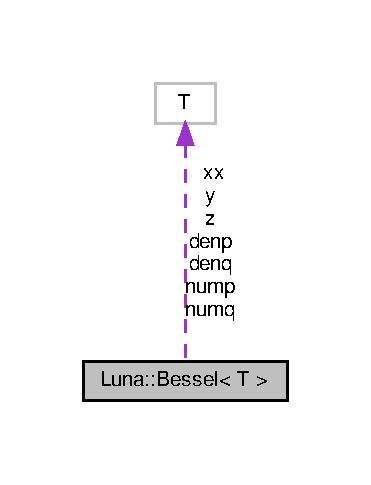
\includegraphics[width=178pt]{structLuna_1_1Bessel__coll__graph}
\end{center}
\end{figure}
\subsection*{Public Member Functions}
\begin{DoxyCompactItemize}
\item 
\hyperlink{structLuna_1_1Bessel_aefa78789b4db0a57f4a6f178ebba1d7f}{Bessel} ()
\item 
void \hyperlink{structLuna_1_1Bessel_aa42218eff6062d962d3fd1287c458583}{rat} (const T x, const double $\ast$r, const double $\ast$s, const int n)
\item 
void \hyperlink{structLuna_1_1Bessel_aaa00a95b752eec29e8c370e17f10f6c0}{asp} (const double $\ast$pn, const double $\ast$pd, const double $\ast$qn, const double $\ast$qd, const double fac)
\item 
T \hyperlink{structLuna_1_1Bessel_a8eeb87d47905d77825276a27ff59de12}{J0} (const T \&x)
\begin{DoxyCompactList}\small\item\em The \hyperlink{structLuna_1_1Bessel}{Bessel} function $ J_0(x) $. \end{DoxyCompactList}\item 
T \hyperlink{structLuna_1_1Bessel_aa9666abfed63d6b97db0b2b776135ef4}{J1} (const T \&x)
\begin{DoxyCompactList}\small\item\em The \hyperlink{structLuna_1_1Bessel}{Bessel} function $ J_1(x) $. \end{DoxyCompactList}\item 
T \hyperlink{structLuna_1_1Bessel_aaa4710f118acafa90f55c1a93b3748da}{Y0} (const T \&x)
\begin{DoxyCompactList}\small\item\em The \hyperlink{structLuna_1_1Bessel}{Bessel} function $ Y_0(x) $. \end{DoxyCompactList}\item 
T \hyperlink{structLuna_1_1Bessel_ab93c15c62695c56fd1d399a00e9a124a}{Y1} (const T \&x)
\begin{DoxyCompactList}\small\item\em The \hyperlink{structLuna_1_1Bessel}{Bessel} function $ Y_1(x) $. \end{DoxyCompactList}\item 
T \hyperlink{structLuna_1_1Bessel_a7df1de7f7173193becc3be8a0c0071a9}{Jn} (const int n, const T \&x)
\begin{DoxyCompactList}\small\item\em The \hyperlink{structLuna_1_1Bessel}{Bessel} function $ J_n(x) $. \end{DoxyCompactList}\item 
T \hyperlink{structLuna_1_1Bessel_aeffbc7ae897573b756c0ddab93ecf6de}{Yn} (const int n, const T \&x)
\begin{DoxyCompactList}\small\item\em The \hyperlink{structLuna_1_1Bessel}{Bessel} function $ Y_n(x) $. \end{DoxyCompactList}\end{DoxyCompactItemize}
\subsection*{Public Attributes}
\begin{DoxyCompactItemize}
\item 
const double \hyperlink{structLuna_1_1Bessel_a69e31bcef81cee0b64a40efd2c6195ac}{xj00}
\item 
const double \hyperlink{structLuna_1_1Bessel_a40044c24955f5e771fd8cbef9fd06397}{xj10}
\item 
const double \hyperlink{structLuna_1_1Bessel_a9423de154e56c25f2615deaa699e1ad2}{xj01}
\item 
const double \hyperlink{structLuna_1_1Bessel_a7120d0fce9cdd7c7f650fb113d56a2ee}{xj11}
\item 
const double \hyperlink{structLuna_1_1Bessel_a4c3a3f91a127b39c913845c77f377c79}{twoopi}
\item 
const double \hyperlink{structLuna_1_1Bessel_a25963b9942422f3d48c0239e8be57f0c}{pio4}
\item 
const double \hyperlink{structLuna_1_1Bessel_a37ddc99f8caaca6814791a3f425370c5}{j0r} \mbox{[}7\mbox{]}
\item 
const double \hyperlink{structLuna_1_1Bessel_a1085d982e9d66d9c29da9798eedb4354}{j0s} \mbox{[}7\mbox{]}
\item 
const double \hyperlink{structLuna_1_1Bessel_aeb87c7ddc34900a7b9dcd123c49c31fe}{j0pn} \mbox{[}5\mbox{]}
\item 
const double \hyperlink{structLuna_1_1Bessel_af55d98ad282898bd505468892ccd1eb1}{j0pd} \mbox{[}5\mbox{]}
\item 
const double \hyperlink{structLuna_1_1Bessel_a5d64c71be5d9ec982587b391a3e2373f}{j0qn} \mbox{[}5\mbox{]}
\item 
const double \hyperlink{structLuna_1_1Bessel_a6f9e1aebe0a5d93388b3b14c67513886}{j0qd} \mbox{[}5\mbox{]}
\item 
const double \hyperlink{structLuna_1_1Bessel_a836feb9b56c106c385d3eb38324f6b2a}{j1r} \mbox{[}7\mbox{]}
\item 
const double \hyperlink{structLuna_1_1Bessel_a70050646ad99739a25c73bcf1d7be60e}{j1s} \mbox{[}7\mbox{]}
\item 
const double \hyperlink{structLuna_1_1Bessel_a0c4696a43b34189116152eac96fd58f1}{j1pn} \mbox{[}5\mbox{]}
\item 
const double \hyperlink{structLuna_1_1Bessel_a5db7fdd8d6855252dfe97b46c073a061}{j1pd} \mbox{[}5\mbox{]}
\item 
const double \hyperlink{structLuna_1_1Bessel_a525e537373d5f47d498981215d270770}{j1qn} \mbox{[}5\mbox{]}
\item 
const double \hyperlink{structLuna_1_1Bessel_a28d43c510a489515508fdf18450a280c}{j1qd} \mbox{[}5\mbox{]}
\item 
const double \hyperlink{structLuna_1_1Bessel_a66915e7a2dd7ef9b2eee1600b272d7a9}{y0r} \mbox{[}9\mbox{]}
\item 
const double \hyperlink{structLuna_1_1Bessel_abff8e2375cf91f57fb3bb71a379f8c20}{y0s} \mbox{[}9\mbox{]}
\item 
const double \hyperlink{structLuna_1_1Bessel_a543af2a1841681067dd1f346819d47dc}{y0pn} \mbox{[}5\mbox{]}
\item 
const double \hyperlink{structLuna_1_1Bessel_aae034512aa17e9a7541b9df1eab88627}{y0pd} \mbox{[}5\mbox{]}
\item 
const double \hyperlink{structLuna_1_1Bessel_a1bcf2ab4b0bfdbf914cc33cb9f6f22be}{y0qn} \mbox{[}5\mbox{]}
\item 
const double \hyperlink{structLuna_1_1Bessel_acc0752d48d86fad96a06178f62fb9780}{y0qd} \mbox{[}5\mbox{]}
\item 
const double \hyperlink{structLuna_1_1Bessel_a558dbb69ececd5b2e46447709c99077e}{y1r} \mbox{[}8\mbox{]}
\item 
const double \hyperlink{structLuna_1_1Bessel_ac2eeeedc9437d9a3b78cd9e30ba2aa37}{y1s} \mbox{[}8\mbox{]}
\item 
const double \hyperlink{structLuna_1_1Bessel_af161635651020ba0c10099888ad348ac}{y1pn} \mbox{[}5\mbox{]}
\item 
const double \hyperlink{structLuna_1_1Bessel_a22637ff3011249c465d3970c92edc83e}{y1pd} \mbox{[}5\mbox{]}
\item 
const double \hyperlink{structLuna_1_1Bessel_ad1bcc14a49575518e9e8227621b39129}{y1qn} \mbox{[}5\mbox{]}
\item 
const double \hyperlink{structLuna_1_1Bessel_a69de10ab8f83dd702c5fbea8b2033e43}{y1qd} \mbox{[}5\mbox{]}
\item 
double \hyperlink{structLuna_1_1Bessel_ace7f3d0a3d4fcca01955bd95cdede89a}{ax}
\item 
T \hyperlink{structLuna_1_1Bessel_a01ee09f3e4275f102df4c3b83fad1776}{nump}
\item 
T \hyperlink{structLuna_1_1Bessel_a71fa71babc245cef7c0902591ed30fff}{denp}
\item 
T \hyperlink{structLuna_1_1Bessel_aa126082495f16ae7d353f0b0623c80b8}{numq}
\item 
T \hyperlink{structLuna_1_1Bessel_a76731982814bd931ae5e8eb725f22c85}{denq}
\item 
T \hyperlink{structLuna_1_1Bessel_a15736ca5396b6f1b87895da22654d522}{xx}
\item 
T \hyperlink{structLuna_1_1Bessel_ab054d5c26284b7736633c171cd2717fc}{y}
\item 
T \hyperlink{structLuna_1_1Bessel_a3ffa857b03c181b3e3ba7422124c60e1}{z}
\end{DoxyCompactItemize}


\subsection{Detailed Description}
\subsubsection*{template$<$typename T$>$\newline
struct Luna\+::\+Bessel$<$ T $>$}



Definition at line 174 of file Special.\+h.



\subsection{Constructor \& Destructor Documentation}
\mbox{\Hypertarget{structLuna_1_1Bessel_aefa78789b4db0a57f4a6f178ebba1d7f}\label{structLuna_1_1Bessel_aefa78789b4db0a57f4a6f178ebba1d7f}} 
\index{Luna\+::\+Bessel@{Luna\+::\+Bessel}!Bessel@{Bessel}}
\index{Bessel@{Bessel}!Luna\+::\+Bessel@{Luna\+::\+Bessel}}
\subsubsection{\texorpdfstring{Bessel()}{Bessel()}}
{\footnotesize\ttfamily template$<$typename T$>$ \\
\hyperlink{structLuna_1_1Bessel}{Luna\+::\+Bessel}$<$ T $>$\+::\hyperlink{structLuna_1_1Bessel}{Bessel} (\begin{DoxyParamCaption}{ }\end{DoxyParamCaption})\hspace{0.3cm}{\ttfamily [inline]}}



Definition at line 241 of file Special.\+h.


\begin{DoxyCode}
241                : \hyperlink{structLuna_1_1Bessel_a69e31bcef81cee0b64a40efd2c6195ac}{xj00}( 5.783185962946785 ),
242                  \hyperlink{structLuna_1_1Bessel_a40044c24955f5e771fd8cbef9fd06397}{xj10}( 3.047126234366209e1 ),
243                  \hyperlink{structLuna_1_1Bessel_a9423de154e56c25f2615deaa699e1ad2}{xj01}( 1.468197064212389e1 ),
244                  \hyperlink{structLuna_1_1Bessel_a7120d0fce9cdd7c7f650fb113d56a2ee}{xj11}( 4.921845632169460e1 ),
245                  \hyperlink{structLuna_1_1Bessel_a4c3a3f91a127b39c913845c77f377c79}{twoopi}( 0.6366197723675813 ),
246                  \hyperlink{structLuna_1_1Bessel_a25963b9942422f3d48c0239e8be57f0c}{pio4}( 0.7853981633974483 )
247       \{
248       \}
\end{DoxyCode}


\subsection{Member Function Documentation}
\mbox{\Hypertarget{structLuna_1_1Bessel_aaa00a95b752eec29e8c370e17f10f6c0}\label{structLuna_1_1Bessel_aaa00a95b752eec29e8c370e17f10f6c0}} 
\index{Luna\+::\+Bessel@{Luna\+::\+Bessel}!asp@{asp}}
\index{asp@{asp}!Luna\+::\+Bessel@{Luna\+::\+Bessel}}
\subsubsection{\texorpdfstring{asp()}{asp()}}
{\footnotesize\ttfamily template$<$typename T$>$ \\
void \hyperlink{structLuna_1_1Bessel}{Luna\+::\+Bessel}$<$ T $>$\+::asp (\begin{DoxyParamCaption}\item[{const double $\ast$}]{pn,  }\item[{const double $\ast$}]{pd,  }\item[{const double $\ast$}]{qn,  }\item[{const double $\ast$}]{qd,  }\item[{const double}]{fac }\end{DoxyParamCaption})\hspace{0.3cm}{\ttfamily [inline]}}



Definition at line 263 of file Special.\+h.



References Luna\+::\+Bessel$<$ T $>$\+::ax, Luna\+::\+Bessel$<$ T $>$\+::pio4, and Luna\+::\+Bessel$<$ T $>$\+::z.



Referenced by Luna\+::\+Bessel$<$ T $>$\+::\+J0(), Luna\+::\+Bessel$<$ T $>$\+::\+J1(), Luna\+::\+Bessel$<$ T $>$\+::\+Y0(), and Luna\+::\+Bessel$<$ T $>$\+::\+Y1().


\begin{DoxyCode}
265       \{
266             \hyperlink{structLuna_1_1Bessel_a3ffa857b03c181b3e3ba7422124c60e1}{z} = 8.0 / \hyperlink{structLuna_1_1Bessel_ace7f3d0a3d4fcca01955bd95cdede89a}{ax};
267             \hyperlink{structLuna_1_1Bessel_ab054d5c26284b7736633c171cd2717fc}{y} = \hyperlink{structLuna_1_1Bessel_a3ffa857b03c181b3e3ba7422124c60e1}{z} * \hyperlink{structLuna_1_1Bessel_a3ffa857b03c181b3e3ba7422124c60e1}{z};
268             \hyperlink{structLuna_1_1Bessel_a15736ca5396b6f1b87895da22654d522}{xx} = \hyperlink{structLuna_1_1Bessel_ace7f3d0a3d4fcca01955bd95cdede89a}{ax} - fac * \hyperlink{structLuna_1_1Bessel_a25963b9942422f3d48c0239e8be57f0c}{pio4};
269             \hyperlink{structLuna_1_1Bessel_a01ee09f3e4275f102df4c3b83fad1776}{nump} = pn[ 4 ];
270             \hyperlink{structLuna_1_1Bessel_a71fa71babc245cef7c0902591ed30fff}{denp} = pd[ 4 ];
271             \hyperlink{structLuna_1_1Bessel_aa126082495f16ae7d353f0b0623c80b8}{numq} = qn[ 4 ];
272             \hyperlink{structLuna_1_1Bessel_a76731982814bd931ae5e8eb725f22c85}{denq} = qd[ 4 ];
273             \textcolor{keywordflow}{for} ( \textcolor{keywordtype}{int} i = 3; i >= 0; i-- )
274         \{
275                 \hyperlink{structLuna_1_1Bessel_a01ee09f3e4275f102df4c3b83fad1776}{nump} = \hyperlink{structLuna_1_1Bessel_a01ee09f3e4275f102df4c3b83fad1776}{nump} * \hyperlink{structLuna_1_1Bessel_ab054d5c26284b7736633c171cd2717fc}{y} + pn[ i ];
276                 \hyperlink{structLuna_1_1Bessel_a71fa71babc245cef7c0902591ed30fff}{denp} = \hyperlink{structLuna_1_1Bessel_a71fa71babc245cef7c0902591ed30fff}{denp} * \hyperlink{structLuna_1_1Bessel_ab054d5c26284b7736633c171cd2717fc}{y} + pd[ i ];
277                 \hyperlink{structLuna_1_1Bessel_aa126082495f16ae7d353f0b0623c80b8}{numq} = \hyperlink{structLuna_1_1Bessel_aa126082495f16ae7d353f0b0623c80b8}{numq} * \hyperlink{structLuna_1_1Bessel_ab054d5c26284b7736633c171cd2717fc}{y} + qn[ i ];
278                 \hyperlink{structLuna_1_1Bessel_a76731982814bd931ae5e8eb725f22c85}{denq} = \hyperlink{structLuna_1_1Bessel_a76731982814bd931ae5e8eb725f22c85}{denq} * \hyperlink{structLuna_1_1Bessel_ab054d5c26284b7736633c171cd2717fc}{y} + qd[ i ];
279             \}
280         \}
\end{DoxyCode}
\mbox{\Hypertarget{structLuna_1_1Bessel_a8eeb87d47905d77825276a27ff59de12}\label{structLuna_1_1Bessel_a8eeb87d47905d77825276a27ff59de12}} 
\index{Luna\+::\+Bessel@{Luna\+::\+Bessel}!J0@{J0}}
\index{J0@{J0}!Luna\+::\+Bessel@{Luna\+::\+Bessel}}
\subsubsection{\texorpdfstring{J0()}{J0()}}
{\footnotesize\ttfamily template$<$typename T$>$ \\
T \hyperlink{structLuna_1_1Bessel}{Luna\+::\+Bessel}$<$ T $>$\+::J0 (\begin{DoxyParamCaption}\item[{const T \&}]{x }\end{DoxyParamCaption})\hspace{0.3cm}{\ttfamily [inline]}}



The \hyperlink{structLuna_1_1Bessel}{Bessel} function $ J_0(x) $. 


\begin{DoxyParams}{Parameters}
{\em x} & The arguement of the function \\
\hline
\end{DoxyParams}
\begin{DoxyReturn}{Returns}
The \hyperlink{structLuna_1_1Bessel}{Bessel} function of the first kind $ J_0(x) $ 
\end{DoxyReturn}


Definition at line 285 of file Special.\+h.



References Luna\+::\+Bessel$<$ T $>$\+::asp(), Luna\+::\+Bessel$<$ T $>$\+::denp, Luna\+::\+Bessel$<$ T $>$\+::denq, Luna\+::\+Bessel$<$ T $>$\+::rat(), and Luna\+::\+Bessel$<$ T $>$\+::xj00.



Referenced by Luna\+::\+Bessel$<$ T $>$\+::\+Jn(), and Luna\+::\+Bessel$<$ T $>$\+::\+Y0().


\begin{DoxyCode}
286       \{
287             \textcolor{keywordflow}{if} ( ( \hyperlink{structLuna_1_1Bessel_ace7f3d0a3d4fcca01955bd95cdede89a}{ax} = abs( std::real(\hyperlink{namespaceHeat__plot_aa88370c16b85b784ccbde3ed88bc1991}{x}) ) ) < 8.0 ) \{
288                 \hyperlink{structLuna_1_1Bessel_aa42218eff6062d962d3fd1287c458583}{rat}( \hyperlink{namespaceHeat__plot_aa88370c16b85b784ccbde3ed88bc1991}{x}, \hyperlink{structLuna_1_1Bessel_a37ddc99f8caaca6814791a3f425370c5}{j0r}, \hyperlink{structLuna_1_1Bessel_a1085d982e9d66d9c29da9798eedb4354}{j0s}, 6 );
289                 \textcolor{keywordflow}{return} \hyperlink{structLuna_1_1Bessel_a01ee09f3e4275f102df4c3b83fad1776}{nump} * ( \hyperlink{structLuna_1_1Bessel_ab054d5c26284b7736633c171cd2717fc}{y} - \hyperlink{structLuna_1_1Bessel_a69e31bcef81cee0b64a40efd2c6195ac}{xj00} ) * ( \hyperlink{structLuna_1_1Bessel_ab054d5c26284b7736633c171cd2717fc}{y} - \hyperlink{structLuna_1_1Bessel_a40044c24955f5e771fd8cbef9fd06397}{xj10} ) / \hyperlink{structLuna_1_1Bessel_a71fa71babc245cef7c0902591ed30fff}{denp};
290             \} \textcolor{keywordflow}{else} \{
291                 \hyperlink{structLuna_1_1Bessel_aaa00a95b752eec29e8c370e17f10f6c0}{asp}( \hyperlink{structLuna_1_1Bessel_aeb87c7ddc34900a7b9dcd123c49c31fe}{j0pn}, \hyperlink{structLuna_1_1Bessel_af55d98ad282898bd505468892ccd1eb1}{j0pd}, \hyperlink{structLuna_1_1Bessel_a5d64c71be5d9ec982587b391a3e2373f}{j0qn}, \hyperlink{structLuna_1_1Bessel_a6f9e1aebe0a5d93388b3b14c67513886}{j0qd}, 1. );
292                 \textcolor{keywordflow}{return} sqrt( \hyperlink{structLuna_1_1Bessel_a4c3a3f91a127b39c913845c77f377c79}{twoopi} / \hyperlink{structLuna_1_1Bessel_ace7f3d0a3d4fcca01955bd95cdede89a}{ax} ) * ( cos( \hyperlink{structLuna_1_1Bessel_a15736ca5396b6f1b87895da22654d522}{xx} ) * \hyperlink{structLuna_1_1Bessel_a01ee09f3e4275f102df4c3b83fad1776}{nump} / 
      \hyperlink{structLuna_1_1Bessel_a71fa71babc245cef7c0902591ed30fff}{denp} - \hyperlink{structLuna_1_1Bessel_a3ffa857b03c181b3e3ba7422124c60e1}{z} * sin( \hyperlink{structLuna_1_1Bessel_a15736ca5396b6f1b87895da22654d522}{xx} )
293                  * \hyperlink{structLuna_1_1Bessel_aa126082495f16ae7d353f0b0623c80b8}{numq} / \hyperlink{structLuna_1_1Bessel_a76731982814bd931ae5e8eb725f22c85}{denq} );
294             \}
295         \}
\end{DoxyCode}
\mbox{\Hypertarget{structLuna_1_1Bessel_aa9666abfed63d6b97db0b2b776135ef4}\label{structLuna_1_1Bessel_aa9666abfed63d6b97db0b2b776135ef4}} 
\index{Luna\+::\+Bessel@{Luna\+::\+Bessel}!J1@{J1}}
\index{J1@{J1}!Luna\+::\+Bessel@{Luna\+::\+Bessel}}
\subsubsection{\texorpdfstring{J1()}{J1()}}
{\footnotesize\ttfamily template$<$typename T$>$ \\
T \hyperlink{structLuna_1_1Bessel}{Luna\+::\+Bessel}$<$ T $>$\+::J1 (\begin{DoxyParamCaption}\item[{const T \&}]{x }\end{DoxyParamCaption})\hspace{0.3cm}{\ttfamily [inline]}}



The \hyperlink{structLuna_1_1Bessel}{Bessel} function $ J_1(x) $. 


\begin{DoxyParams}{Parameters}
{\em x} & The arguement of the function \\
\hline
\end{DoxyParams}
\begin{DoxyReturn}{Returns}
The \hyperlink{structLuna_1_1Bessel}{Bessel} function of the first kind $ J_1(x) $ 
\end{DoxyReturn}


Definition at line 300 of file Special.\+h.



References Luna\+::\+Bessel$<$ T $>$\+::asp(), Luna\+::\+Bessel$<$ T $>$\+::denp, Luna\+::\+Bessel$<$ T $>$\+::denq, Luna\+::\+Bessel$<$ T $>$\+::rat(), and Luna\+::\+Bessel$<$ T $>$\+::xj01.



Referenced by Luna\+::\+Bessel$<$ T $>$\+::\+Jn(), and Luna\+::\+Bessel$<$ T $>$\+::\+Y1().


\begin{DoxyCode}
300                          \{
301             \textcolor{keywordflow}{if} ( ( \hyperlink{structLuna_1_1Bessel_ace7f3d0a3d4fcca01955bd95cdede89a}{ax} = abs( std::real(\hyperlink{namespaceHeat__plot_aa88370c16b85b784ccbde3ed88bc1991}{x}) ) ) < 8.0 ) \{
302                 \hyperlink{structLuna_1_1Bessel_aa42218eff6062d962d3fd1287c458583}{rat}( \hyperlink{namespaceHeat__plot_aa88370c16b85b784ccbde3ed88bc1991}{x}, \hyperlink{structLuna_1_1Bessel_a836feb9b56c106c385d3eb38324f6b2a}{j1r}, \hyperlink{structLuna_1_1Bessel_a70050646ad99739a25c73bcf1d7be60e}{j1s}, 6 );
303                 \textcolor{keywordflow}{return} \hyperlink{namespaceHeat__plot_aa88370c16b85b784ccbde3ed88bc1991}{x} * \hyperlink{structLuna_1_1Bessel_a01ee09f3e4275f102df4c3b83fad1776}{nump} * ( \hyperlink{structLuna_1_1Bessel_ab054d5c26284b7736633c171cd2717fc}{y} - \hyperlink{structLuna_1_1Bessel_a9423de154e56c25f2615deaa699e1ad2}{xj01} ) * ( \hyperlink{structLuna_1_1Bessel_ab054d5c26284b7736633c171cd2717fc}{y} - \hyperlink{structLuna_1_1Bessel_a7120d0fce9cdd7c7f650fb113d56a2ee}{xj11} ) / 
      \hyperlink{structLuna_1_1Bessel_a71fa71babc245cef7c0902591ed30fff}{denp};
304             \} \textcolor{keywordflow}{else} \{
305                 \hyperlink{structLuna_1_1Bessel_aaa00a95b752eec29e8c370e17f10f6c0}{asp}( \hyperlink{structLuna_1_1Bessel_a0c4696a43b34189116152eac96fd58f1}{j1pn}, \hyperlink{structLuna_1_1Bessel_a5db7fdd8d6855252dfe97b46c073a061}{j1pd}, \hyperlink{structLuna_1_1Bessel_a525e537373d5f47d498981215d270770}{j1qn}, \hyperlink{structLuna_1_1Bessel_a28d43c510a489515508fdf18450a280c}{j1qd}, 3. );
306                 T ans = sqrt( \hyperlink{structLuna_1_1Bessel_a4c3a3f91a127b39c913845c77f377c79}{twoopi} / \hyperlink{structLuna_1_1Bessel_ace7f3d0a3d4fcca01955bd95cdede89a}{ax} ) * ( cos( \hyperlink{structLuna_1_1Bessel_a15736ca5396b6f1b87895da22654d522}{xx} ) * \hyperlink{structLuna_1_1Bessel_a01ee09f3e4275f102df4c3b83fad1776}{nump} / 
      \hyperlink{structLuna_1_1Bessel_a71fa71babc245cef7c0902591ed30fff}{denp}
307                        - \hyperlink{structLuna_1_1Bessel_a3ffa857b03c181b3e3ba7422124c60e1}{z} * sin( \hyperlink{structLuna_1_1Bessel_a15736ca5396b6f1b87895da22654d522}{xx} ) * \hyperlink{structLuna_1_1Bessel_aa126082495f16ae7d353f0b0623c80b8}{numq} / \hyperlink{structLuna_1_1Bessel_a76731982814bd931ae5e8eb725f22c85}{denq} );
308                 \textcolor{keywordflow}{return} std::real( \hyperlink{namespaceHeat__plot_aa88370c16b85b784ccbde3ed88bc1991}{x} ) > 0.0 ? ans : -ans;
309             \}
310         \}
\end{DoxyCode}
\mbox{\Hypertarget{structLuna_1_1Bessel_a7df1de7f7173193becc3be8a0c0071a9}\label{structLuna_1_1Bessel_a7df1de7f7173193becc3be8a0c0071a9}} 
\index{Luna\+::\+Bessel@{Luna\+::\+Bessel}!Jn@{Jn}}
\index{Jn@{Jn}!Luna\+::\+Bessel@{Luna\+::\+Bessel}}
\subsubsection{\texorpdfstring{Jn()}{Jn()}}
{\footnotesize\ttfamily template$<$typename T$>$ \\
T \hyperlink{structLuna_1_1Bessel}{Luna\+::\+Bessel}$<$ T $>$\+::Jn (\begin{DoxyParamCaption}\item[{const int}]{n,  }\item[{const T \&}]{x }\end{DoxyParamCaption})\hspace{0.3cm}{\ttfamily [inline]}}



The \hyperlink{structLuna_1_1Bessel}{Bessel} function $ J_n(x) $. 


\begin{DoxyParams}{Parameters}
{\em n} & The \hyperlink{structLuna_1_1Bessel}{Bessel} function number (integer) \\
\hline
{\em x} & The arguement of the function \\
\hline
\end{DoxyParams}
\begin{DoxyReturn}{Returns}
The \hyperlink{structLuna_1_1Bessel}{Bessel} function of the first kind $ J_n(x) $ 
\end{DoxyReturn}


Definition at line 348 of file Special.\+h.



References Luna\+::\+Bessel$<$ T $>$\+::ax, Heat\+\_\+plot\+::int, Luna\+::\+Bessel$<$ T $>$\+::\+J0(), Luna\+::\+Bessel$<$ T $>$\+::\+J1(), and Heat\+\_\+plot\+::x.


\begin{DoxyCode}
349       \{
350         \textcolor{keyword}{const} \textcolor{keywordtype}{double} ACC = 160.0;
351         \textcolor{keyword}{const} \textcolor{keywordtype}{int} IEXP = std::numeric\_limits<T>::max\_exponent / 2;
352         \textcolor{keywordtype}{bool} jsum;
353         \textcolor{keywordtype}{int} j , k, m;
354         T bj , bjm, bjp, dum, sum, tox, ans;
355         \textcolor{keywordtype}{double} \hyperlink{structLuna_1_1Bessel_ace7f3d0a3d4fcca01955bd95cdede89a}{ax};
356 
357         \textcolor{keywordflow}{if} (n==0) \textcolor{keywordflow}{return} \hyperlink{structLuna_1_1Bessel_a8eeb87d47905d77825276a27ff59de12}{J0}(\hyperlink{namespaceHeat__plot_aa88370c16b85b784ccbde3ed88bc1991}{x});
358         \textcolor{keywordflow}{if} (n==1) \textcolor{keywordflow}{return} \hyperlink{structLuna_1_1Bessel_aa9666abfed63d6b97db0b2b776135ef4}{J1}(\hyperlink{namespaceHeat__plot_aa88370c16b85b784ccbde3ed88bc1991}{x});
359         \textcolor{comment}{// ax=abs(x);}
360         ax = abs( std::real( \hyperlink{namespaceHeat__plot_aa88370c16b85b784ccbde3ed88bc1991}{x} ) );
361         \textcolor{keywordflow}{if} ( ax * ax <= 8.0 * std::numeric\_limits<double>::min() ) \textcolor{keywordflow}{return} 0.0;
362         \textcolor{keywordflow}{else} \textcolor{keywordflow}{if} ( ax > \textcolor{keywordtype}{double}( n ) ) \{
363             \textcolor{comment}{//tox=2.0/ax;}
364             \textcolor{comment}{//bjm=J0(ax);}
365             \textcolor{comment}{//bj=J1(ax);}
366           tox = 2.0 / \hyperlink{namespaceHeat__plot_aa88370c16b85b784ccbde3ed88bc1991}{x};
367           bjm = \hyperlink{structLuna_1_1Bessel_a8eeb87d47905d77825276a27ff59de12}{J0}( \hyperlink{namespaceHeat__plot_aa88370c16b85b784ccbde3ed88bc1991}{x} );
368           bj = \hyperlink{structLuna_1_1Bessel_aa9666abfed63d6b97db0b2b776135ef4}{J1}( \hyperlink{namespaceHeat__plot_aa88370c16b85b784ccbde3ed88bc1991}{x} );
369             \textcolor{keywordflow}{for} ( j = 1; j < n; j++ ) \{
370                 bjp = 1. * j * tox * bj - bjm;
371                 bjm = bj;
372                 bj = bjp;
373             \}
374             ans = bj;
375         \} \textcolor{keywordflow}{else} \{
376             \textcolor{comment}{//tox=2.0/ax;}
377           tox = 2.0 / \hyperlink{namespaceHeat__plot_aa88370c16b85b784ccbde3ed88bc1991}{x};
378             m = 2 * ( ( n + \hyperlink{namespaceHeat__plot_ac721620fed23609e47f849d804f29546}{int}( sqrt( ACC * n ) ) ) / 2 );
379             jsum=\textcolor{keyword}{false};
380             bjp=ans=sum=0.0;
381             bj=1.0;
382             \textcolor{keywordflow}{for} ( j = m; j > 0; j-- ) \{
383                 bjm = 1. * j * tox * bj - bjp;
384                 bjp = bj;
385                 bj = bjm;
386                 dum.real( frexp( std::real( bj ), &k ) );
387                 \textcolor{keywordflow}{if} (k > IEXP) \{
388                     bj.real( ldexp( std::real( bj ), -IEXP ) );
389                     bjp.real( ldexp( std::real( bjp ), -IEXP ) );
390                     ans.real( ldexp( std::real( ans ), -IEXP ) );
391                     sum.real( ldexp( std::real( sum ), -IEXP ) );
392                 \}
393             dum.imag( frexp( std::imag( bj ), &k ) );
394                 \textcolor{keywordflow}{if} (k > IEXP) \{
395                     bj.imag( ldexp( std::imag( bj ), -IEXP ) );
396                     bjp.imag( ldexp( std::imag( bjp ), -IEXP ) );
397                     ans.imag( ldexp( std::imag( ans ), -IEXP ) );
398                     sum.imag( ldexp( std::imag( sum ), -IEXP ) );
399                 \}
400                 \textcolor{keywordflow}{if} ( jsum ) sum += bj;
401                 jsum =! jsum;
402                 \textcolor{keywordflow}{if} (j == n) ans = bjp;
403             \}
404             sum = 2.0 * sum - bj;
405             ans /= sum;
406         \}
407         \textcolor{keywordflow}{return} std::real( \hyperlink{namespaceHeat__plot_aa88370c16b85b784ccbde3ed88bc1991}{x} ) < 0.0 && (n & 1) ? -ans : ans;
408       \}
\end{DoxyCode}
\mbox{\Hypertarget{structLuna_1_1Bessel_aa42218eff6062d962d3fd1287c458583}\label{structLuna_1_1Bessel_aa42218eff6062d962d3fd1287c458583}} 
\index{Luna\+::\+Bessel@{Luna\+::\+Bessel}!rat@{rat}}
\index{rat@{rat}!Luna\+::\+Bessel@{Luna\+::\+Bessel}}
\subsubsection{\texorpdfstring{rat()}{rat()}}
{\footnotesize\ttfamily template$<$typename T$>$ \\
void \hyperlink{structLuna_1_1Bessel}{Luna\+::\+Bessel}$<$ T $>$\+::rat (\begin{DoxyParamCaption}\item[{const T}]{x,  }\item[{const double $\ast$}]{r,  }\item[{const double $\ast$}]{s,  }\item[{const int}]{n }\end{DoxyParamCaption})\hspace{0.3cm}{\ttfamily [inline]}}



Definition at line 250 of file Special.\+h.



References Heat\+\_\+plot\+::x, and Luna\+::\+Bessel$<$ T $>$\+::y.



Referenced by Luna\+::\+Bessel$<$ T $>$\+::\+J0(), Luna\+::\+Bessel$<$ T $>$\+::\+J1(), Luna\+::\+Bessel$<$ T $>$\+::\+Y0(), and Luna\+::\+Bessel$<$ T $>$\+::\+Y1().


\begin{DoxyCode}
251       \{
252             \hyperlink{structLuna_1_1Bessel_ab054d5c26284b7736633c171cd2717fc}{y} = \hyperlink{namespaceHeat__plot_aa88370c16b85b784ccbde3ed88bc1991}{x} * \hyperlink{namespaceHeat__plot_aa88370c16b85b784ccbde3ed88bc1991}{x};
253             \hyperlink{structLuna_1_1Bessel_a3ffa857b03c181b3e3ba7422124c60e1}{z} = 64.0 - \hyperlink{structLuna_1_1Bessel_ab054d5c26284b7736633c171cd2717fc}{y};
254             \hyperlink{structLuna_1_1Bessel_a01ee09f3e4275f102df4c3b83fad1776}{nump} = r[ n ];
255             \hyperlink{structLuna_1_1Bessel_a71fa71babc245cef7c0902591ed30fff}{denp} = s[ n ];
256             \textcolor{keywordflow}{for} ( \textcolor{keywordtype}{int} i = n-1; i >= 0; i-- )
257         \{
258                 \hyperlink{structLuna_1_1Bessel_a01ee09f3e4275f102df4c3b83fad1776}{nump} = \hyperlink{structLuna_1_1Bessel_a01ee09f3e4275f102df4c3b83fad1776}{nump} * \hyperlink{structLuna_1_1Bessel_a3ffa857b03c181b3e3ba7422124c60e1}{z} + r[ i ];
259                 \hyperlink{structLuna_1_1Bessel_a71fa71babc245cef7c0902591ed30fff}{denp} = \hyperlink{structLuna_1_1Bessel_a71fa71babc245cef7c0902591ed30fff}{denp} * \hyperlink{structLuna_1_1Bessel_ab054d5c26284b7736633c171cd2717fc}{y} + s[ i ];
260             \}
261         \}
\end{DoxyCode}
\mbox{\Hypertarget{structLuna_1_1Bessel_aaa4710f118acafa90f55c1a93b3748da}\label{structLuna_1_1Bessel_aaa4710f118acafa90f55c1a93b3748da}} 
\index{Luna\+::\+Bessel@{Luna\+::\+Bessel}!Y0@{Y0}}
\index{Y0@{Y0}!Luna\+::\+Bessel@{Luna\+::\+Bessel}}
\subsubsection{\texorpdfstring{Y0()}{Y0()}}
{\footnotesize\ttfamily template$<$typename T$>$ \\
T \hyperlink{structLuna_1_1Bessel}{Luna\+::\+Bessel}$<$ T $>$\+::Y0 (\begin{DoxyParamCaption}\item[{const T \&}]{x }\end{DoxyParamCaption})\hspace{0.3cm}{\ttfamily [inline]}}



The \hyperlink{structLuna_1_1Bessel}{Bessel} function $ Y_0(x) $. 


\begin{DoxyParams}{Parameters}
{\em x} & The arguement of the function \\
\hline
\end{DoxyParams}
\begin{DoxyReturn}{Returns}
The \hyperlink{structLuna_1_1Bessel}{Bessel} function of the second kind $ Y_0(x) $ 
\end{DoxyReturn}


Definition at line 315 of file Special.\+h.



References Luna\+::\+Bessel$<$ T $>$\+::asp(), Luna\+::\+Bessel$<$ T $>$\+::denq, Luna\+::\+Bessel$<$ T $>$\+::\+J0(), and Luna\+::\+Bessel$<$ T $>$\+::rat().



Referenced by Luna\+::\+Bessel$<$ T $>$\+::\+Yn().


\begin{DoxyCode}
315                          \{
316             \textcolor{keywordflow}{if} ( std::real( \hyperlink{namespaceHeat__plot_aa88370c16b85b784ccbde3ed88bc1991}{x} ) < 8.0) \{
317                 T j0x = \hyperlink{structLuna_1_1Bessel_a8eeb87d47905d77825276a27ff59de12}{J0}( \hyperlink{namespaceHeat__plot_aa88370c16b85b784ccbde3ed88bc1991}{x} );
318                 \hyperlink{structLuna_1_1Bessel_aa42218eff6062d962d3fd1287c458583}{rat}( \hyperlink{namespaceHeat__plot_aa88370c16b85b784ccbde3ed88bc1991}{x}, \hyperlink{structLuna_1_1Bessel_a66915e7a2dd7ef9b2eee1600b272d7a9}{y0r}, \hyperlink{structLuna_1_1Bessel_abff8e2375cf91f57fb3bb71a379f8c20}{y0s}, 8 );
319                 \textcolor{keywordflow}{return} \hyperlink{structLuna_1_1Bessel_a01ee09f3e4275f102df4c3b83fad1776}{nump} / \hyperlink{structLuna_1_1Bessel_a71fa71babc245cef7c0902591ed30fff}{denp} + \hyperlink{structLuna_1_1Bessel_a4c3a3f91a127b39c913845c77f377c79}{twoopi} * j0x * log( \hyperlink{namespaceHeat__plot_aa88370c16b85b784ccbde3ed88bc1991}{x} );
320             \} \textcolor{keywordflow}{else} \{
321                 \hyperlink{structLuna_1_1Bessel_ace7f3d0a3d4fcca01955bd95cdede89a}{ax} = std::real( \hyperlink{namespaceHeat__plot_aa88370c16b85b784ccbde3ed88bc1991}{x} );
322                 \hyperlink{structLuna_1_1Bessel_aaa00a95b752eec29e8c370e17f10f6c0}{asp}( \hyperlink{structLuna_1_1Bessel_a543af2a1841681067dd1f346819d47dc}{y0pn}, \hyperlink{structLuna_1_1Bessel_aae034512aa17e9a7541b9df1eab88627}{y0pd}, \hyperlink{structLuna_1_1Bessel_a1bcf2ab4b0bfdbf914cc33cb9f6f22be}{y0qn}, \hyperlink{structLuna_1_1Bessel_acc0752d48d86fad96a06178f62fb9780}{y0qd}, 1. );
323                 \textcolor{keywordflow}{return} sqrt( \hyperlink{structLuna_1_1Bessel_a4c3a3f91a127b39c913845c77f377c79}{twoopi} / \hyperlink{namespaceHeat__plot_aa88370c16b85b784ccbde3ed88bc1991}{x} ) * ( sin( \hyperlink{structLuna_1_1Bessel_a15736ca5396b6f1b87895da22654d522}{xx} ) * \hyperlink{structLuna_1_1Bessel_a01ee09f3e4275f102df4c3b83fad1776}{nump} / 
      \hyperlink{structLuna_1_1Bessel_a71fa71babc245cef7c0902591ed30fff}{denp}
324                  + \hyperlink{structLuna_1_1Bessel_a3ffa857b03c181b3e3ba7422124c60e1}{z} * cos( \hyperlink{structLuna_1_1Bessel_a15736ca5396b6f1b87895da22654d522}{xx} ) * \hyperlink{structLuna_1_1Bessel_aa126082495f16ae7d353f0b0623c80b8}{numq} / \hyperlink{structLuna_1_1Bessel_a76731982814bd931ae5e8eb725f22c85}{denq} );
325             \}
326         \}
\end{DoxyCode}
\mbox{\Hypertarget{structLuna_1_1Bessel_ab93c15c62695c56fd1d399a00e9a124a}\label{structLuna_1_1Bessel_ab93c15c62695c56fd1d399a00e9a124a}} 
\index{Luna\+::\+Bessel@{Luna\+::\+Bessel}!Y1@{Y1}}
\index{Y1@{Y1}!Luna\+::\+Bessel@{Luna\+::\+Bessel}}
\subsubsection{\texorpdfstring{Y1()}{Y1()}}
{\footnotesize\ttfamily template$<$typename T$>$ \\
T \hyperlink{structLuna_1_1Bessel}{Luna\+::\+Bessel}$<$ T $>$\+::Y1 (\begin{DoxyParamCaption}\item[{const T \&}]{x }\end{DoxyParamCaption})\hspace{0.3cm}{\ttfamily [inline]}}



The \hyperlink{structLuna_1_1Bessel}{Bessel} function $ Y_1(x) $. 


\begin{DoxyParams}{Parameters}
{\em x} & The arguement of the function \\
\hline
\end{DoxyParams}
\begin{DoxyReturn}{Returns}
The \hyperlink{structLuna_1_1Bessel}{Bessel} function of the second kind $ Y_1(x) $ 
\end{DoxyReturn}


Definition at line 331 of file Special.\+h.



References Luna\+::\+Bessel$<$ T $>$\+::asp(), Luna\+::\+Bessel$<$ T $>$\+::denq, Luna\+::\+Bessel$<$ T $>$\+::\+J1(), Luna\+::\+Bessel$<$ T $>$\+::rat(), and Heat\+\_\+plot\+::x.



Referenced by Luna\+::\+Bessel$<$ T $>$\+::\+Yn().


\begin{DoxyCode}
331                          \{
332             \textcolor{keywordflow}{if} ( std::real( \hyperlink{namespaceHeat__plot_aa88370c16b85b784ccbde3ed88bc1991}{x} ) < 8.0 ) \{
333                 T j1x = \hyperlink{structLuna_1_1Bessel_aa9666abfed63d6b97db0b2b776135ef4}{J1}( \hyperlink{namespaceHeat__plot_aa88370c16b85b784ccbde3ed88bc1991}{x} );
334                 \hyperlink{structLuna_1_1Bessel_aa42218eff6062d962d3fd1287c458583}{rat}( \hyperlink{namespaceHeat__plot_aa88370c16b85b784ccbde3ed88bc1991}{x}, \hyperlink{structLuna_1_1Bessel_a558dbb69ececd5b2e46447709c99077e}{y1r}, \hyperlink{structLuna_1_1Bessel_ac2eeeedc9437d9a3b78cd9e30ba2aa37}{y1s}, 7 );
335                 \textcolor{keywordflow}{return} \hyperlink{namespaceHeat__plot_aa88370c16b85b784ccbde3ed88bc1991}{x} * \hyperlink{structLuna_1_1Bessel_a01ee09f3e4275f102df4c3b83fad1776}{nump} / \hyperlink{structLuna_1_1Bessel_a71fa71babc245cef7c0902591ed30fff}{denp} + \hyperlink{structLuna_1_1Bessel_a4c3a3f91a127b39c913845c77f377c79}{twoopi} * ( j1x * log( \hyperlink{namespaceHeat__plot_aa88370c16b85b784ccbde3ed88bc1991}{x} ) - 1.0 / 
      \hyperlink{namespaceHeat__plot_aa88370c16b85b784ccbde3ed88bc1991}{x} );
336             \} \textcolor{keywordflow}{else} \{
337                 \hyperlink{structLuna_1_1Bessel_ace7f3d0a3d4fcca01955bd95cdede89a}{ax} = std::real( \hyperlink{namespaceHeat__plot_aa88370c16b85b784ccbde3ed88bc1991}{x} );
338                 \hyperlink{structLuna_1_1Bessel_aaa00a95b752eec29e8c370e17f10f6c0}{asp}( \hyperlink{structLuna_1_1Bessel_af161635651020ba0c10099888ad348ac}{y1pn}, \hyperlink{structLuna_1_1Bessel_a22637ff3011249c465d3970c92edc83e}{y1pd}, \hyperlink{structLuna_1_1Bessel_ad1bcc14a49575518e9e8227621b39129}{y1qn}, \hyperlink{structLuna_1_1Bessel_a69de10ab8f83dd702c5fbea8b2033e43}{y1qd}, 3. );
339                 \textcolor{keywordflow}{return} sqrt( \hyperlink{structLuna_1_1Bessel_a4c3a3f91a127b39c913845c77f377c79}{twoopi} / \hyperlink{namespaceHeat__plot_aa88370c16b85b784ccbde3ed88bc1991}{x} ) * ( sin( \hyperlink{structLuna_1_1Bessel_a15736ca5396b6f1b87895da22654d522}{xx} ) * \hyperlink{structLuna_1_1Bessel_a01ee09f3e4275f102df4c3b83fad1776}{nump} / 
      \hyperlink{structLuna_1_1Bessel_a71fa71babc245cef7c0902591ed30fff}{denp}
340                  + \hyperlink{structLuna_1_1Bessel_a3ffa857b03c181b3e3ba7422124c60e1}{z} * cos( \hyperlink{structLuna_1_1Bessel_a15736ca5396b6f1b87895da22654d522}{xx} ) * \hyperlink{structLuna_1_1Bessel_aa126082495f16ae7d353f0b0623c80b8}{numq} / \hyperlink{structLuna_1_1Bessel_a76731982814bd931ae5e8eb725f22c85}{denq} );
341             \}
342         \}
\end{DoxyCode}
\mbox{\Hypertarget{structLuna_1_1Bessel_aeffbc7ae897573b756c0ddab93ecf6de}\label{structLuna_1_1Bessel_aeffbc7ae897573b756c0ddab93ecf6de}} 
\index{Luna\+::\+Bessel@{Luna\+::\+Bessel}!Yn@{Yn}}
\index{Yn@{Yn}!Luna\+::\+Bessel@{Luna\+::\+Bessel}}
\subsubsection{\texorpdfstring{Yn()}{Yn()}}
{\footnotesize\ttfamily template$<$typename T$>$ \\
T \hyperlink{structLuna_1_1Bessel}{Luna\+::\+Bessel}$<$ T $>$\+::Yn (\begin{DoxyParamCaption}\item[{const int}]{n,  }\item[{const T \&}]{x }\end{DoxyParamCaption})\hspace{0.3cm}{\ttfamily [inline]}}



The \hyperlink{structLuna_1_1Bessel}{Bessel} function $ Y_n(x) $. 


\begin{DoxyParams}{Parameters}
{\em n} & The \hyperlink{structLuna_1_1Bessel}{Bessel} function number (integer) \\
\hline
{\em x} & The arguement of the function \\
\hline
\end{DoxyParams}
\begin{DoxyReturn}{Returns}
The \hyperlink{structLuna_1_1Bessel}{Bessel} function of the second kind $ Y_n(x) $ 
\end{DoxyReturn}


Definition at line 414 of file Special.\+h.



References Heat\+\_\+plot\+::x, Luna\+::\+Bessel$<$ T $>$\+::\+Y0(), and Luna\+::\+Bessel$<$ T $>$\+::\+Y1().



Referenced by main().


\begin{DoxyCode}
415       \{
416         \textcolor{keywordtype}{int} j;
417         T by, bym, byp, tox;
418         \textcolor{keywordflow}{if} ( n == 0 ) \textcolor{keywordflow}{return} \hyperlink{structLuna_1_1Bessel_aaa4710f118acafa90f55c1a93b3748da}{Y0}( \hyperlink{namespaceHeat__plot_aa88370c16b85b784ccbde3ed88bc1991}{x} );
419         \textcolor{keywordflow}{if} ( n == 1 ) \textcolor{keywordflow}{return} \hyperlink{structLuna_1_1Bessel_ab93c15c62695c56fd1d399a00e9a124a}{Y1}( \hyperlink{namespaceHeat__plot_aa88370c16b85b784ccbde3ed88bc1991}{x} );
420         tox = 2.0 / \hyperlink{namespaceHeat__plot_aa88370c16b85b784ccbde3ed88bc1991}{x};
421         by = \hyperlink{structLuna_1_1Bessel_ab93c15c62695c56fd1d399a00e9a124a}{Y1}( \hyperlink{namespaceHeat__plot_aa88370c16b85b784ccbde3ed88bc1991}{x} );
422         bym = \hyperlink{structLuna_1_1Bessel_aaa4710f118acafa90f55c1a93b3748da}{Y0}( \hyperlink{namespaceHeat__plot_aa88370c16b85b784ccbde3ed88bc1991}{x} );
423         \textcolor{keywordflow}{for} ( j = 1; j < n; j++ ) \{
424             byp =1. * j * tox * by - bym;
425             bym = by;
426             by = byp;
427         \}
428         \textcolor{keywordflow}{return} by;
429       \}
\end{DoxyCode}


\subsection{Member Data Documentation}
\mbox{\Hypertarget{structLuna_1_1Bessel_ace7f3d0a3d4fcca01955bd95cdede89a}\label{structLuna_1_1Bessel_ace7f3d0a3d4fcca01955bd95cdede89a}} 
\index{Luna\+::\+Bessel@{Luna\+::\+Bessel}!ax@{ax}}
\index{ax@{ax}!Luna\+::\+Bessel@{Luna\+::\+Bessel}}
\subsubsection{\texorpdfstring{ax}{ax}}
{\footnotesize\ttfamily template$<$typename T$>$ \\
double \hyperlink{structLuna_1_1Bessel}{Luna\+::\+Bessel}$<$ T $>$\+::ax}



Definition at line 238 of file Special.\+h.



Referenced by Luna\+::\+Bessel$<$ T $>$\+::asp(), and Luna\+::\+Bessel$<$ T $>$\+::\+Jn().

\mbox{\Hypertarget{structLuna_1_1Bessel_a71fa71babc245cef7c0902591ed30fff}\label{structLuna_1_1Bessel_a71fa71babc245cef7c0902591ed30fff}} 
\index{Luna\+::\+Bessel@{Luna\+::\+Bessel}!denp@{denp}}
\index{denp@{denp}!Luna\+::\+Bessel@{Luna\+::\+Bessel}}
\subsubsection{\texorpdfstring{denp}{denp}}
{\footnotesize\ttfamily template$<$typename T$>$ \\
T \hyperlink{structLuna_1_1Bessel}{Luna\+::\+Bessel}$<$ T $>$\+::denp}



Definition at line 239 of file Special.\+h.



Referenced by Luna\+::\+Bessel$<$ T $>$\+::\+J0(), and Luna\+::\+Bessel$<$ T $>$\+::\+J1().

\mbox{\Hypertarget{structLuna_1_1Bessel_a76731982814bd931ae5e8eb725f22c85}\label{structLuna_1_1Bessel_a76731982814bd931ae5e8eb725f22c85}} 
\index{Luna\+::\+Bessel@{Luna\+::\+Bessel}!denq@{denq}}
\index{denq@{denq}!Luna\+::\+Bessel@{Luna\+::\+Bessel}}
\subsubsection{\texorpdfstring{denq}{denq}}
{\footnotesize\ttfamily template$<$typename T$>$ \\
T \hyperlink{structLuna_1_1Bessel}{Luna\+::\+Bessel}$<$ T $>$\+::denq}



Definition at line 239 of file Special.\+h.



Referenced by Luna\+::\+Bessel$<$ T $>$\+::\+J0(), Luna\+::\+Bessel$<$ T $>$\+::\+J1(), Luna\+::\+Bessel$<$ T $>$\+::\+Y0(), and Luna\+::\+Bessel$<$ T $>$\+::\+Y1().

\mbox{\Hypertarget{structLuna_1_1Bessel_af55d98ad282898bd505468892ccd1eb1}\label{structLuna_1_1Bessel_af55d98ad282898bd505468892ccd1eb1}} 
\index{Luna\+::\+Bessel@{Luna\+::\+Bessel}!j0pd@{j0pd}}
\index{j0pd@{j0pd}!Luna\+::\+Bessel@{Luna\+::\+Bessel}}
\subsubsection{\texorpdfstring{j0pd}{j0pd}}
{\footnotesize\ttfamily template$<$typename T$>$ \\
const double \hyperlink{structLuna_1_1Bessel}{Luna\+::\+Bessel}$<$ T $>$\+::j0pd\mbox{[}5\mbox{]}}

{\bfseries Initial value\+:}
\begin{DoxyCode}
=\{1.0,1.040797262528109,2.588070904043728e-1,
        1.529954477721284e-2,1.168931211650012e-4\}
\end{DoxyCode}


Definition at line 184 of file Special.\+h.

\mbox{\Hypertarget{structLuna_1_1Bessel_aeb87c7ddc34900a7b9dcd123c49c31fe}\label{structLuna_1_1Bessel_aeb87c7ddc34900a7b9dcd123c49c31fe}} 
\index{Luna\+::\+Bessel@{Luna\+::\+Bessel}!j0pn@{j0pn}}
\index{j0pn@{j0pn}!Luna\+::\+Bessel@{Luna\+::\+Bessel}}
\subsubsection{\texorpdfstring{j0pn}{j0pn}}
{\footnotesize\ttfamily template$<$typename T$>$ \\
const double \hyperlink{structLuna_1_1Bessel}{Luna\+::\+Bessel}$<$ T $>$\+::j0pn\mbox{[}5\mbox{]}}

{\bfseries Initial value\+:}
\begin{DoxyCode}
=\{9.999999999999999e-1,1.039698629715637,
        2.576910172633398e-1,1.504152485749669e-2,1.052598413585270e-4\}
\end{DoxyCode}


Definition at line 182 of file Special.\+h.

\mbox{\Hypertarget{structLuna_1_1Bessel_a6f9e1aebe0a5d93388b3b14c67513886}\label{structLuna_1_1Bessel_a6f9e1aebe0a5d93388b3b14c67513886}} 
\index{Luna\+::\+Bessel@{Luna\+::\+Bessel}!j0qd@{j0qd}}
\index{j0qd@{j0qd}!Luna\+::\+Bessel@{Luna\+::\+Bessel}}
\subsubsection{\texorpdfstring{j0qd}{j0qd}}
{\footnotesize\ttfamily template$<$typename T$>$ \\
const double \hyperlink{structLuna_1_1Bessel}{Luna\+::\+Bessel}$<$ T $>$\+::j0qd\mbox{[}5\mbox{]}}

{\bfseries Initial value\+:}
\begin{DoxyCode}
=\{1.0,1.237980436358390,3.838793938147116e-1,
        3.100323481550864e-2,4.165515825072393e-4\}
\end{DoxyCode}


Definition at line 188 of file Special.\+h.

\mbox{\Hypertarget{structLuna_1_1Bessel_a5d64c71be5d9ec982587b391a3e2373f}\label{structLuna_1_1Bessel_a5d64c71be5d9ec982587b391a3e2373f}} 
\index{Luna\+::\+Bessel@{Luna\+::\+Bessel}!j0qn@{j0qn}}
\index{j0qn@{j0qn}!Luna\+::\+Bessel@{Luna\+::\+Bessel}}
\subsubsection{\texorpdfstring{j0qn}{j0qn}}
{\footnotesize\ttfamily template$<$typename T$>$ \\
const double \hyperlink{structLuna_1_1Bessel}{Luna\+::\+Bessel}$<$ T $>$\+::j0qn\mbox{[}5\mbox{]}}

{\bfseries Initial value\+:}
\begin{DoxyCode}
=\{-1.562499999999992e-2,-1.920039317065641e-2,
        -5.827951791963418e-3,-4.372674978482726e-4,-3.895839560412374e-6\}
\end{DoxyCode}


Definition at line 186 of file Special.\+h.

\mbox{\Hypertarget{structLuna_1_1Bessel_a37ddc99f8caaca6814791a3f425370c5}\label{structLuna_1_1Bessel_a37ddc99f8caaca6814791a3f425370c5}} 
\index{Luna\+::\+Bessel@{Luna\+::\+Bessel}!j0r@{j0r}}
\index{j0r@{j0r}!Luna\+::\+Bessel@{Luna\+::\+Bessel}}
\subsubsection{\texorpdfstring{j0r}{j0r}}
{\footnotesize\ttfamily template$<$typename T$>$ \\
const double \hyperlink{structLuna_1_1Bessel}{Luna\+::\+Bessel}$<$ T $>$\+::j0r\mbox{[}7\mbox{]}}

{\bfseries Initial value\+:}
\begin{DoxyCode}
=\{1.682397144220462e-4,2.058861258868952e-5,
        5.288947320067750e-7,5.557173907680151e-9,2.865540042042604e-11,
        7.398972674152181e-14,7.925088479679688e-17\}
\end{DoxyCode}


Definition at line 176 of file Special.\+h.

\mbox{\Hypertarget{structLuna_1_1Bessel_a1085d982e9d66d9c29da9798eedb4354}\label{structLuna_1_1Bessel_a1085d982e9d66d9c29da9798eedb4354}} 
\index{Luna\+::\+Bessel@{Luna\+::\+Bessel}!j0s@{j0s}}
\index{j0s@{j0s}!Luna\+::\+Bessel@{Luna\+::\+Bessel}}
\subsubsection{\texorpdfstring{j0s}{j0s}}
{\footnotesize\ttfamily template$<$typename T$>$ \\
const double \hyperlink{structLuna_1_1Bessel}{Luna\+::\+Bessel}$<$ T $>$\+::j0s\mbox{[}7\mbox{]}}

{\bfseries Initial value\+:}
\begin{DoxyCode}
=\{1.0,1.019685405805929e-2,5.130296867064666e-5,
        1.659702063950243e-7,3.728997574317067e-10,
        5.709292619977798e-13,4.932979170744996e-16\}
\end{DoxyCode}


Definition at line 179 of file Special.\+h.

\mbox{\Hypertarget{structLuna_1_1Bessel_a5db7fdd8d6855252dfe97b46c073a061}\label{structLuna_1_1Bessel_a5db7fdd8d6855252dfe97b46c073a061}} 
\index{Luna\+::\+Bessel@{Luna\+::\+Bessel}!j1pd@{j1pd}}
\index{j1pd@{j1pd}!Luna\+::\+Bessel@{Luna\+::\+Bessel}}
\subsubsection{\texorpdfstring{j1pd}{j1pd}}
{\footnotesize\ttfamily template$<$typename T$>$ \\
const double \hyperlink{structLuna_1_1Bessel}{Luna\+::\+Bessel}$<$ T $>$\+::j1pd\mbox{[}5\mbox{]}}

{\bfseries Initial value\+:}
\begin{DoxyCode}
=\{1.0,1.012208056357845,2.408580305488938e-1,
        1.309511056184273e-2,7.746422941504713e-5\}
\end{DoxyCode}


Definition at line 199 of file Special.\+h.

\mbox{\Hypertarget{structLuna_1_1Bessel_a0c4696a43b34189116152eac96fd58f1}\label{structLuna_1_1Bessel_a0c4696a43b34189116152eac96fd58f1}} 
\index{Luna\+::\+Bessel@{Luna\+::\+Bessel}!j1pn@{j1pn}}
\index{j1pn@{j1pn}!Luna\+::\+Bessel@{Luna\+::\+Bessel}}
\subsubsection{\texorpdfstring{j1pn}{j1pn}}
{\footnotesize\ttfamily template$<$typename T$>$ \\
const double \hyperlink{structLuna_1_1Bessel}{Luna\+::\+Bessel}$<$ T $>$\+::j1pn\mbox{[}5\mbox{]}}

{\bfseries Initial value\+:}
\begin{DoxyCode}
=\{1.0,1.014039111045313,2.426762348629863e-1,
        1.350308200342000e-2,9.516522033988099e-5\}
\end{DoxyCode}


Definition at line 197 of file Special.\+h.

\mbox{\Hypertarget{structLuna_1_1Bessel_a28d43c510a489515508fdf18450a280c}\label{structLuna_1_1Bessel_a28d43c510a489515508fdf18450a280c}} 
\index{Luna\+::\+Bessel@{Luna\+::\+Bessel}!j1qd@{j1qd}}
\index{j1qd@{j1qd}!Luna\+::\+Bessel@{Luna\+::\+Bessel}}
\subsubsection{\texorpdfstring{j1qd}{j1qd}}
{\footnotesize\ttfamily template$<$typename T$>$ \\
const double \hyperlink{structLuna_1_1Bessel}{Luna\+::\+Bessel}$<$ T $>$\+::j1qd\mbox{[}5\mbox{]}}

{\bfseries Initial value\+:}
\begin{DoxyCode}
=\{1.0,1.210119370463693,3.626494789275638e-1,
        2.761695824829316e-2,3.240517192670181e-4\}
\end{DoxyCode}


Definition at line 203 of file Special.\+h.

\mbox{\Hypertarget{structLuna_1_1Bessel_a525e537373d5f47d498981215d270770}\label{structLuna_1_1Bessel_a525e537373d5f47d498981215d270770}} 
\index{Luna\+::\+Bessel@{Luna\+::\+Bessel}!j1qn@{j1qn}}
\index{j1qn@{j1qn}!Luna\+::\+Bessel@{Luna\+::\+Bessel}}
\subsubsection{\texorpdfstring{j1qn}{j1qn}}
{\footnotesize\ttfamily template$<$typename T$>$ \\
const double \hyperlink{structLuna_1_1Bessel}{Luna\+::\+Bessel}$<$ T $>$\+::j1qn\mbox{[}5\mbox{]}}

{\bfseries Initial value\+:}
\begin{DoxyCode}
=\{4.687499999999991e-2,5.652407388406023e-2,
        1.676531273460512e-2,1.231216817715814e-3,1.178364381441801e-5\}
\end{DoxyCode}


Definition at line 201 of file Special.\+h.

\mbox{\Hypertarget{structLuna_1_1Bessel_a836feb9b56c106c385d3eb38324f6b2a}\label{structLuna_1_1Bessel_a836feb9b56c106c385d3eb38324f6b2a}} 
\index{Luna\+::\+Bessel@{Luna\+::\+Bessel}!j1r@{j1r}}
\index{j1r@{j1r}!Luna\+::\+Bessel@{Luna\+::\+Bessel}}
\subsubsection{\texorpdfstring{j1r}{j1r}}
{\footnotesize\ttfamily template$<$typename T$>$ \\
const double \hyperlink{structLuna_1_1Bessel}{Luna\+::\+Bessel}$<$ T $>$\+::j1r\mbox{[}7\mbox{]}}

{\bfseries Initial value\+:}
\begin{DoxyCode}
=\{7.309637831891357e-5,3.551248884746503e-6,
        5.820673901730427e-8,4.500650342170622e-10,1.831596352149641e-12,
        3.891583573305035e-15,3.524978592527982e-18\}
\end{DoxyCode}


Definition at line 191 of file Special.\+h.

\mbox{\Hypertarget{structLuna_1_1Bessel_a70050646ad99739a25c73bcf1d7be60e}\label{structLuna_1_1Bessel_a70050646ad99739a25c73bcf1d7be60e}} 
\index{Luna\+::\+Bessel@{Luna\+::\+Bessel}!j1s@{j1s}}
\index{j1s@{j1s}!Luna\+::\+Bessel@{Luna\+::\+Bessel}}
\subsubsection{\texorpdfstring{j1s}{j1s}}
{\footnotesize\ttfamily template$<$typename T$>$ \\
const double \hyperlink{structLuna_1_1Bessel}{Luna\+::\+Bessel}$<$ T $>$\+::j1s\mbox{[}7\mbox{]}}

{\bfseries Initial value\+:}
\begin{DoxyCode}
=\{1.0,9.398354768446072e-3,4.328946737100230e-5,
        1.271526296341915e-7,2.566305357932989e-10,
        3.477378203574266e-13,2.593535427519985e-16\}
\end{DoxyCode}


Definition at line 194 of file Special.\+h.

\mbox{\Hypertarget{structLuna_1_1Bessel_a01ee09f3e4275f102df4c3b83fad1776}\label{structLuna_1_1Bessel_a01ee09f3e4275f102df4c3b83fad1776}} 
\index{Luna\+::\+Bessel@{Luna\+::\+Bessel}!nump@{nump}}
\index{nump@{nump}!Luna\+::\+Bessel@{Luna\+::\+Bessel}}
\subsubsection{\texorpdfstring{nump}{nump}}
{\footnotesize\ttfamily template$<$typename T$>$ \\
T \hyperlink{structLuna_1_1Bessel}{Luna\+::\+Bessel}$<$ T $>$\+::nump}



Definition at line 239 of file Special.\+h.

\mbox{\Hypertarget{structLuna_1_1Bessel_aa126082495f16ae7d353f0b0623c80b8}\label{structLuna_1_1Bessel_aa126082495f16ae7d353f0b0623c80b8}} 
\index{Luna\+::\+Bessel@{Luna\+::\+Bessel}!numq@{numq}}
\index{numq@{numq}!Luna\+::\+Bessel@{Luna\+::\+Bessel}}
\subsubsection{\texorpdfstring{numq}{numq}}
{\footnotesize\ttfamily template$<$typename T$>$ \\
T \hyperlink{structLuna_1_1Bessel}{Luna\+::\+Bessel}$<$ T $>$\+::numq}



Definition at line 239 of file Special.\+h.

\mbox{\Hypertarget{structLuna_1_1Bessel_a25963b9942422f3d48c0239e8be57f0c}\label{structLuna_1_1Bessel_a25963b9942422f3d48c0239e8be57f0c}} 
\index{Luna\+::\+Bessel@{Luna\+::\+Bessel}!pio4@{pio4}}
\index{pio4@{pio4}!Luna\+::\+Bessel@{Luna\+::\+Bessel}}
\subsubsection{\texorpdfstring{pio4}{pio4}}
{\footnotesize\ttfamily template$<$typename T$>$ \\
const double \hyperlink{structLuna_1_1Bessel}{Luna\+::\+Bessel}$<$ T $>$\+::pio4}



Definition at line 175 of file Special.\+h.



Referenced by Luna\+::\+Bessel$<$ T $>$\+::asp().

\mbox{\Hypertarget{structLuna_1_1Bessel_a4c3a3f91a127b39c913845c77f377c79}\label{structLuna_1_1Bessel_a4c3a3f91a127b39c913845c77f377c79}} 
\index{Luna\+::\+Bessel@{Luna\+::\+Bessel}!twoopi@{twoopi}}
\index{twoopi@{twoopi}!Luna\+::\+Bessel@{Luna\+::\+Bessel}}
\subsubsection{\texorpdfstring{twoopi}{twoopi}}
{\footnotesize\ttfamily template$<$typename T$>$ \\
const double \hyperlink{structLuna_1_1Bessel}{Luna\+::\+Bessel}$<$ T $>$\+::twoopi}



Definition at line 175 of file Special.\+h.

\mbox{\Hypertarget{structLuna_1_1Bessel_a69e31bcef81cee0b64a40efd2c6195ac}\label{structLuna_1_1Bessel_a69e31bcef81cee0b64a40efd2c6195ac}} 
\index{Luna\+::\+Bessel@{Luna\+::\+Bessel}!xj00@{xj00}}
\index{xj00@{xj00}!Luna\+::\+Bessel@{Luna\+::\+Bessel}}
\subsubsection{\texorpdfstring{xj00}{xj00}}
{\footnotesize\ttfamily template$<$typename T$>$ \\
const double \hyperlink{structLuna_1_1Bessel}{Luna\+::\+Bessel}$<$ T $>$\+::xj00}



Definition at line 175 of file Special.\+h.



Referenced by Luna\+::\+Bessel$<$ T $>$\+::\+J0().

\mbox{\Hypertarget{structLuna_1_1Bessel_a9423de154e56c25f2615deaa699e1ad2}\label{structLuna_1_1Bessel_a9423de154e56c25f2615deaa699e1ad2}} 
\index{Luna\+::\+Bessel@{Luna\+::\+Bessel}!xj01@{xj01}}
\index{xj01@{xj01}!Luna\+::\+Bessel@{Luna\+::\+Bessel}}
\subsubsection{\texorpdfstring{xj01}{xj01}}
{\footnotesize\ttfamily template$<$typename T$>$ \\
const double \hyperlink{structLuna_1_1Bessel}{Luna\+::\+Bessel}$<$ T $>$\+::xj01}



Definition at line 175 of file Special.\+h.



Referenced by Luna\+::\+Bessel$<$ T $>$\+::\+J1().

\mbox{\Hypertarget{structLuna_1_1Bessel_a40044c24955f5e771fd8cbef9fd06397}\label{structLuna_1_1Bessel_a40044c24955f5e771fd8cbef9fd06397}} 
\index{Luna\+::\+Bessel@{Luna\+::\+Bessel}!xj10@{xj10}}
\index{xj10@{xj10}!Luna\+::\+Bessel@{Luna\+::\+Bessel}}
\subsubsection{\texorpdfstring{xj10}{xj10}}
{\footnotesize\ttfamily template$<$typename T$>$ \\
const double \hyperlink{structLuna_1_1Bessel}{Luna\+::\+Bessel}$<$ T $>$\+::xj10}



Definition at line 175 of file Special.\+h.

\mbox{\Hypertarget{structLuna_1_1Bessel_a7120d0fce9cdd7c7f650fb113d56a2ee}\label{structLuna_1_1Bessel_a7120d0fce9cdd7c7f650fb113d56a2ee}} 
\index{Luna\+::\+Bessel@{Luna\+::\+Bessel}!xj11@{xj11}}
\index{xj11@{xj11}!Luna\+::\+Bessel@{Luna\+::\+Bessel}}
\subsubsection{\texorpdfstring{xj11}{xj11}}
{\footnotesize\ttfamily template$<$typename T$>$ \\
const double \hyperlink{structLuna_1_1Bessel}{Luna\+::\+Bessel}$<$ T $>$\+::xj11}



Definition at line 175 of file Special.\+h.

\mbox{\Hypertarget{structLuna_1_1Bessel_a15736ca5396b6f1b87895da22654d522}\label{structLuna_1_1Bessel_a15736ca5396b6f1b87895da22654d522}} 
\index{Luna\+::\+Bessel@{Luna\+::\+Bessel}!xx@{xx}}
\index{xx@{xx}!Luna\+::\+Bessel@{Luna\+::\+Bessel}}
\subsubsection{\texorpdfstring{xx}{xx}}
{\footnotesize\ttfamily template$<$typename T$>$ \\
T \hyperlink{structLuna_1_1Bessel}{Luna\+::\+Bessel}$<$ T $>$\+::xx}



Definition at line 239 of file Special.\+h.

\mbox{\Hypertarget{structLuna_1_1Bessel_ab054d5c26284b7736633c171cd2717fc}\label{structLuna_1_1Bessel_ab054d5c26284b7736633c171cd2717fc}} 
\index{Luna\+::\+Bessel@{Luna\+::\+Bessel}!y@{y}}
\index{y@{y}!Luna\+::\+Bessel@{Luna\+::\+Bessel}}
\subsubsection{\texorpdfstring{y}{y}}
{\footnotesize\ttfamily template$<$typename T$>$ \\
T \hyperlink{structLuna_1_1Bessel}{Luna\+::\+Bessel}$<$ T $>$\+::y}



Definition at line 239 of file Special.\+h.



Referenced by Luna\+::\+Bessel$<$ T $>$\+::rat().

\mbox{\Hypertarget{structLuna_1_1Bessel_aae034512aa17e9a7541b9df1eab88627}\label{structLuna_1_1Bessel_aae034512aa17e9a7541b9df1eab88627}} 
\index{Luna\+::\+Bessel@{Luna\+::\+Bessel}!y0pd@{y0pd}}
\index{y0pd@{y0pd}!Luna\+::\+Bessel@{Luna\+::\+Bessel}}
\subsubsection{\texorpdfstring{y0pd}{y0pd}}
{\footnotesize\ttfamily template$<$typename T$>$ \\
const double \hyperlink{structLuna_1_1Bessel}{Luna\+::\+Bessel}$<$ T $>$\+::y0pd\mbox{[}5\mbox{]}}

{\bfseries Initial value\+:}
\begin{DoxyCode}
=\{1.0,1.040797262528109,2.588070904043728e-1,
        1.529954477721284e-2,1.168931211650012e-4\}
\end{DoxyCode}


Definition at line 215 of file Special.\+h.

\mbox{\Hypertarget{structLuna_1_1Bessel_a543af2a1841681067dd1f346819d47dc}\label{structLuna_1_1Bessel_a543af2a1841681067dd1f346819d47dc}} 
\index{Luna\+::\+Bessel@{Luna\+::\+Bessel}!y0pn@{y0pn}}
\index{y0pn@{y0pn}!Luna\+::\+Bessel@{Luna\+::\+Bessel}}
\subsubsection{\texorpdfstring{y0pn}{y0pn}}
{\footnotesize\ttfamily template$<$typename T$>$ \\
const double \hyperlink{structLuna_1_1Bessel}{Luna\+::\+Bessel}$<$ T $>$\+::y0pn\mbox{[}5\mbox{]}}

{\bfseries Initial value\+:}
\begin{DoxyCode}
=\{9.999999999999999e-1,1.039698629715637,
        2.576910172633398e-1,1.504152485749669e-2,1.052598413585270e-4\}
\end{DoxyCode}


Definition at line 213 of file Special.\+h.

\mbox{\Hypertarget{structLuna_1_1Bessel_acc0752d48d86fad96a06178f62fb9780}\label{structLuna_1_1Bessel_acc0752d48d86fad96a06178f62fb9780}} 
\index{Luna\+::\+Bessel@{Luna\+::\+Bessel}!y0qd@{y0qd}}
\index{y0qd@{y0qd}!Luna\+::\+Bessel@{Luna\+::\+Bessel}}
\subsubsection{\texorpdfstring{y0qd}{y0qd}}
{\footnotesize\ttfamily template$<$typename T$>$ \\
const double \hyperlink{structLuna_1_1Bessel}{Luna\+::\+Bessel}$<$ T $>$\+::y0qd\mbox{[}5\mbox{]}}

{\bfseries Initial value\+:}
\begin{DoxyCode}
=\{1.0,1.237980436358390,3.838793938147116e-1,
        3.100323481550864e-2,4.165515825072393e-4\}
\end{DoxyCode}


Definition at line 219 of file Special.\+h.

\mbox{\Hypertarget{structLuna_1_1Bessel_a1bcf2ab4b0bfdbf914cc33cb9f6f22be}\label{structLuna_1_1Bessel_a1bcf2ab4b0bfdbf914cc33cb9f6f22be}} 
\index{Luna\+::\+Bessel@{Luna\+::\+Bessel}!y0qn@{y0qn}}
\index{y0qn@{y0qn}!Luna\+::\+Bessel@{Luna\+::\+Bessel}}
\subsubsection{\texorpdfstring{y0qn}{y0qn}}
{\footnotesize\ttfamily template$<$typename T$>$ \\
const double \hyperlink{structLuna_1_1Bessel}{Luna\+::\+Bessel}$<$ T $>$\+::y0qn\mbox{[}5\mbox{]}}

{\bfseries Initial value\+:}
\begin{DoxyCode}
=\{-1.562499999999992e-2,-1.920039317065641e-2,
        -5.827951791963418e-3,-4.372674978482726e-4,-3.895839560412374e-6\}
\end{DoxyCode}


Definition at line 217 of file Special.\+h.

\mbox{\Hypertarget{structLuna_1_1Bessel_a66915e7a2dd7ef9b2eee1600b272d7a9}\label{structLuna_1_1Bessel_a66915e7a2dd7ef9b2eee1600b272d7a9}} 
\index{Luna\+::\+Bessel@{Luna\+::\+Bessel}!y0r@{y0r}}
\index{y0r@{y0r}!Luna\+::\+Bessel@{Luna\+::\+Bessel}}
\subsubsection{\texorpdfstring{y0r}{y0r}}
{\footnotesize\ttfamily template$<$typename T$>$ \\
const double \hyperlink{structLuna_1_1Bessel}{Luna\+::\+Bessel}$<$ T $>$\+::y0r\mbox{[}9\mbox{]}}

{\bfseries Initial value\+:}
\begin{DoxyCode}
=\{-7.653778457189104e-3,-5.854760129990403e-2,
        3.720671300654721e-4,3.313722284628089e-5,4.247761237036536e-8,
        -4.134562661019613e-9,-3.382190331837473e-11,
        -1.017764126587862e-13,-1.107646382675456e-16\}
\end{DoxyCode}


Definition at line 206 of file Special.\+h.

\mbox{\Hypertarget{structLuna_1_1Bessel_abff8e2375cf91f57fb3bb71a379f8c20}\label{structLuna_1_1Bessel_abff8e2375cf91f57fb3bb71a379f8c20}} 
\index{Luna\+::\+Bessel@{Luna\+::\+Bessel}!y0s@{y0s}}
\index{y0s@{y0s}!Luna\+::\+Bessel@{Luna\+::\+Bessel}}
\subsubsection{\texorpdfstring{y0s}{y0s}}
{\footnotesize\ttfamily template$<$typename T$>$ \\
const double \hyperlink{structLuna_1_1Bessel}{Luna\+::\+Bessel}$<$ T $>$\+::y0s\mbox{[}9\mbox{]}}

{\bfseries Initial value\+:}
\begin{DoxyCode}
=\{1.0,1.125494540257841e-2,6.427210537081400e-5,
        2.462520624294959e-7,7.029372432344291e-10,1.560784108184928e-12,
        2.702374957564761e-15,3.468496737915257e-18,2.716600180811817e-21\}
\end{DoxyCode}


Definition at line 210 of file Special.\+h.

\mbox{\Hypertarget{structLuna_1_1Bessel_a22637ff3011249c465d3970c92edc83e}\label{structLuna_1_1Bessel_a22637ff3011249c465d3970c92edc83e}} 
\index{Luna\+::\+Bessel@{Luna\+::\+Bessel}!y1pd@{y1pd}}
\index{y1pd@{y1pd}!Luna\+::\+Bessel@{Luna\+::\+Bessel}}
\subsubsection{\texorpdfstring{y1pd}{y1pd}}
{\footnotesize\ttfamily template$<$typename T$>$ \\
const double \hyperlink{structLuna_1_1Bessel}{Luna\+::\+Bessel}$<$ T $>$\+::y1pd\mbox{[}5\mbox{]}}

{\bfseries Initial value\+:}
\begin{DoxyCode}
=\{1.0,1.012208056357845,2.408580305488938e-1,
        1.309511056184273e-2,7.746422941504713e-5\}
\end{DoxyCode}


Definition at line 231 of file Special.\+h.

\mbox{\Hypertarget{structLuna_1_1Bessel_af161635651020ba0c10099888ad348ac}\label{structLuna_1_1Bessel_af161635651020ba0c10099888ad348ac}} 
\index{Luna\+::\+Bessel@{Luna\+::\+Bessel}!y1pn@{y1pn}}
\index{y1pn@{y1pn}!Luna\+::\+Bessel@{Luna\+::\+Bessel}}
\subsubsection{\texorpdfstring{y1pn}{y1pn}}
{\footnotesize\ttfamily template$<$typename T$>$ \\
const double \hyperlink{structLuna_1_1Bessel}{Luna\+::\+Bessel}$<$ T $>$\+::y1pn\mbox{[}5\mbox{]}}

{\bfseries Initial value\+:}
\begin{DoxyCode}
=\{1.0,1.014039111045313,2.426762348629863e-1,
        1.350308200342000e-2,9.516522033988099e-5\}
\end{DoxyCode}


Definition at line 229 of file Special.\+h.

\mbox{\Hypertarget{structLuna_1_1Bessel_a69de10ab8f83dd702c5fbea8b2033e43}\label{structLuna_1_1Bessel_a69de10ab8f83dd702c5fbea8b2033e43}} 
\index{Luna\+::\+Bessel@{Luna\+::\+Bessel}!y1qd@{y1qd}}
\index{y1qd@{y1qd}!Luna\+::\+Bessel@{Luna\+::\+Bessel}}
\subsubsection{\texorpdfstring{y1qd}{y1qd}}
{\footnotesize\ttfamily template$<$typename T$>$ \\
const double \hyperlink{structLuna_1_1Bessel}{Luna\+::\+Bessel}$<$ T $>$\+::y1qd\mbox{[}5\mbox{]}}

{\bfseries Initial value\+:}
\begin{DoxyCode}
=\{1.0,1.210119370463693,3.626494789275638e-1,
        2.761695824829316e-2,3.240517192670181e-4\}
\end{DoxyCode}


Definition at line 235 of file Special.\+h.

\mbox{\Hypertarget{structLuna_1_1Bessel_ad1bcc14a49575518e9e8227621b39129}\label{structLuna_1_1Bessel_ad1bcc14a49575518e9e8227621b39129}} 
\index{Luna\+::\+Bessel@{Luna\+::\+Bessel}!y1qn@{y1qn}}
\index{y1qn@{y1qn}!Luna\+::\+Bessel@{Luna\+::\+Bessel}}
\subsubsection{\texorpdfstring{y1qn}{y1qn}}
{\footnotesize\ttfamily template$<$typename T$>$ \\
const double \hyperlink{structLuna_1_1Bessel}{Luna\+::\+Bessel}$<$ T $>$\+::y1qn\mbox{[}5\mbox{]}}

{\bfseries Initial value\+:}
\begin{DoxyCode}
=\{4.687499999999991e-2,5.652407388406023e-2,
        1.676531273460512e-2,1.231216817715814e-3,1.178364381441801e-5\}
\end{DoxyCode}


Definition at line 233 of file Special.\+h.

\mbox{\Hypertarget{structLuna_1_1Bessel_a558dbb69ececd5b2e46447709c99077e}\label{structLuna_1_1Bessel_a558dbb69ececd5b2e46447709c99077e}} 
\index{Luna\+::\+Bessel@{Luna\+::\+Bessel}!y1r@{y1r}}
\index{y1r@{y1r}!Luna\+::\+Bessel@{Luna\+::\+Bessel}}
\subsubsection{\texorpdfstring{y1r}{y1r}}
{\footnotesize\ttfamily template$<$typename T$>$ \\
const double \hyperlink{structLuna_1_1Bessel}{Luna\+::\+Bessel}$<$ T $>$\+::y1r\mbox{[}8\mbox{]}}

{\bfseries Initial value\+:}
\begin{DoxyCode}
=\{-1.041835425863234e-1,-1.135093963908952e-5,
        2.212118520638132e-4,1.270981874287763e-6,
        -3.982892100836748e-8,-4.820712110115943e-10,
        -1.929392690596969e-12,-2.725259514545605e-15\}
\end{DoxyCode}


Definition at line 222 of file Special.\+h.

\mbox{\Hypertarget{structLuna_1_1Bessel_ac2eeeedc9437d9a3b78cd9e30ba2aa37}\label{structLuna_1_1Bessel_ac2eeeedc9437d9a3b78cd9e30ba2aa37}} 
\index{Luna\+::\+Bessel@{Luna\+::\+Bessel}!y1s@{y1s}}
\index{y1s@{y1s}!Luna\+::\+Bessel@{Luna\+::\+Bessel}}
\subsubsection{\texorpdfstring{y1s}{y1s}}
{\footnotesize\ttfamily template$<$typename T$>$ \\
const double \hyperlink{structLuna_1_1Bessel}{Luna\+::\+Bessel}$<$ T $>$\+::y1s\mbox{[}8\mbox{]}}

{\bfseries Initial value\+:}
\begin{DoxyCode}
=\{1.0,1.186694184425838e-2,7.121205411175519e-5,
        2.847142454085055e-7,8.364240962784899e-10,1.858128283833724e-12,
        3.018846060781846e-15,3.015798735815980e-18\}
\end{DoxyCode}


Definition at line 226 of file Special.\+h.

\mbox{\Hypertarget{structLuna_1_1Bessel_a3ffa857b03c181b3e3ba7422124c60e1}\label{structLuna_1_1Bessel_a3ffa857b03c181b3e3ba7422124c60e1}} 
\index{Luna\+::\+Bessel@{Luna\+::\+Bessel}!z@{z}}
\index{z@{z}!Luna\+::\+Bessel@{Luna\+::\+Bessel}}
\subsubsection{\texorpdfstring{z}{z}}
{\footnotesize\ttfamily template$<$typename T$>$ \\
T \hyperlink{structLuna_1_1Bessel}{Luna\+::\+Bessel}$<$ T $>$\+::z}



Definition at line 239 of file Special.\+h.



Referenced by Luna\+::\+Bessel$<$ T $>$\+::asp().



The documentation for this struct was generated from the following file\+:\begin{DoxyCompactItemize}
\item 
include/\+Luna/\hyperlink{Special_8h}{Special.\+h}\end{DoxyCompactItemize}

\hypertarget{classLuna_1_1Equation}{}\section{Luna\+:\+:Equation$<$ T, X $>$ Class Template Reference}
\label{classLuna_1_1Equation}\index{Luna\+::\+Equation$<$ T, X $>$@{Luna\+::\+Equation$<$ T, X $>$}}


{\ttfamily \#include $<$Equation.\+h$>$}



Inheritance diagram for Luna\+:\+:Equation$<$ T, X $>$\+:\nopagebreak
\begin{figure}[H]
\begin{center}
\leavevmode
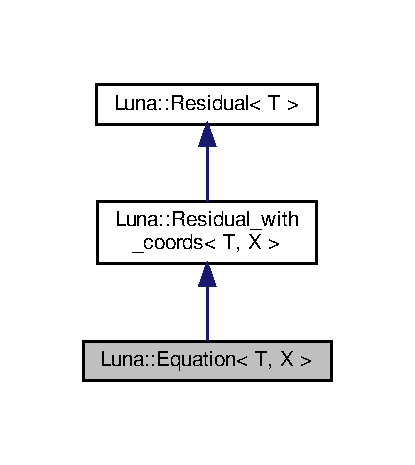
\includegraphics[width=199pt]{classLuna_1_1Equation__inherit__graph}
\end{center}
\end{figure}


Collaboration diagram for Luna\+:\+:Equation$<$ T, X $>$\+:\nopagebreak
\begin{figure}[H]
\begin{center}
\leavevmode
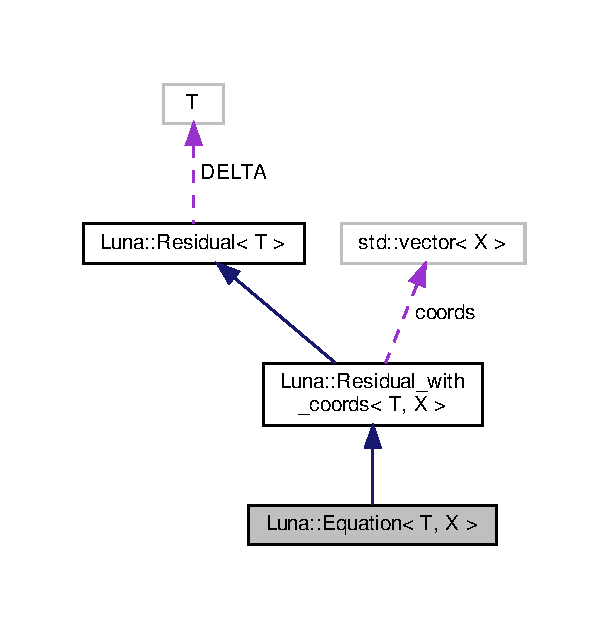
\includegraphics[width=292pt]{classLuna_1_1Equation__coll__graph}
\end{center}
\end{figure}
\subsection*{Public Member Functions}
\begin{DoxyCompactItemize}
\item 
\hyperlink{classLuna_1_1Equation_a3331703c98854fe27f0108d75f794942}{Equation} (const unsigned \&order)
\begin{DoxyCompactList}\small\item\em Constructor for equation class. \end{DoxyCompactList}\item 
virtual \hyperlink{classLuna_1_1Equation_accb94fee3ccd30bc1075374c4b257564}{$\sim$\+Equation} ()
\begin{DoxyCompactList}\small\item\em An empty destructor, virtual since we have virtual methods. \end{DoxyCompactList}\end{DoxyCompactItemize}
\subsection*{Additional Inherited Members}


\subsection{Detailed Description}
\subsubsection*{template$<$class T, class X = double$>$\newline
class Luna\+::\+Equation$<$ T, X $>$}



Definition at line 22 of file Equation.\+h.



\subsection{Constructor \& Destructor Documentation}
\mbox{\Hypertarget{classLuna_1_1Equation_a3331703c98854fe27f0108d75f794942}\label{classLuna_1_1Equation_a3331703c98854fe27f0108d75f794942}} 
\index{Luna\+::\+Equation@{Luna\+::\+Equation}!Equation@{Equation}}
\index{Equation@{Equation}!Luna\+::\+Equation@{Luna\+::\+Equation}}
\subsubsection{\texorpdfstring{Equation()}{Equation()}}
{\footnotesize\ttfamily template$<$typename T , typename X $>$ \\
\hyperlink{classLuna_1_1Equation}{Luna\+::\+Equation}$<$ T, X $>$\+::\hyperlink{classLuna_1_1Equation}{Equation} (\begin{DoxyParamCaption}\item[{const unsigned \&}]{order }\end{DoxyParamCaption})}



Constructor for equation class. 


\begin{DoxyParams}{Parameters}
{\em order} & The order of the system \\
\hline
\end{DoxyParams}


Definition at line 35 of file Equation.\+h.


\begin{DoxyCode}
35                                                   :
36       Residual\_with\_coords<T, X>( order, 1 )
37   \{
38   \}
\end{DoxyCode}
\mbox{\Hypertarget{classLuna_1_1Equation_accb94fee3ccd30bc1075374c4b257564}\label{classLuna_1_1Equation_accb94fee3ccd30bc1075374c4b257564}} 
\index{Luna\+::\+Equation@{Luna\+::\+Equation}!````~Equation@{$\sim$\+Equation}}
\index{````~Equation@{$\sim$\+Equation}!Luna\+::\+Equation@{Luna\+::\+Equation}}
\subsubsection{\texorpdfstring{$\sim$\+Equation()}{~Equation()}}
{\footnotesize\ttfamily template$<$typename T , typename X $>$ \\
\hyperlink{classLuna_1_1Equation}{Luna\+::\+Equation}$<$ T, X $>$\+::$\sim$\hyperlink{classLuna_1_1Equation}{Equation} (\begin{DoxyParamCaption}{ }\end{DoxyParamCaption})\hspace{0.3cm}{\ttfamily [virtual]}}



An empty destructor, virtual since we have virtual methods. 



Definition at line 41 of file Equation.\+h.


\begin{DoxyCode}
42   \{
43   \}
\end{DoxyCode}


The documentation for this class was generated from the following file\+:\begin{DoxyCompactItemize}
\item 
include/\+Luna/\hyperlink{Equation_8h}{Equation.\+h}\end{DoxyCompactItemize}

\hypertarget{classLuna_1_1Equation__1matrix}{}\section{Luna\+:\+:Equation\+\_\+1matrix$<$ T, X $>$ Class Template Reference}
\label{classLuna_1_1Equation__1matrix}\index{Luna\+::\+Equation\+\_\+1matrix$<$ T, X $>$@{Luna\+::\+Equation\+\_\+1matrix$<$ T, X $>$}}


{\ttfamily \#include $<$Equation\+\_\+1matrix.\+h$>$}



Inheritance diagram for Luna\+:\+:Equation\+\_\+1matrix$<$ T, X $>$\+:\nopagebreak
\begin{figure}[H]
\begin{center}
\leavevmode
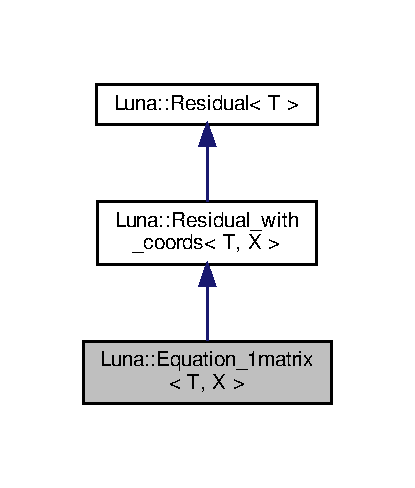
\includegraphics[width=199pt]{classLuna_1_1Equation__1matrix__inherit__graph}
\end{center}
\end{figure}


Collaboration diagram for Luna\+:\+:Equation\+\_\+1matrix$<$ T, X $>$\+:\nopagebreak
\begin{figure}[H]
\begin{center}
\leavevmode
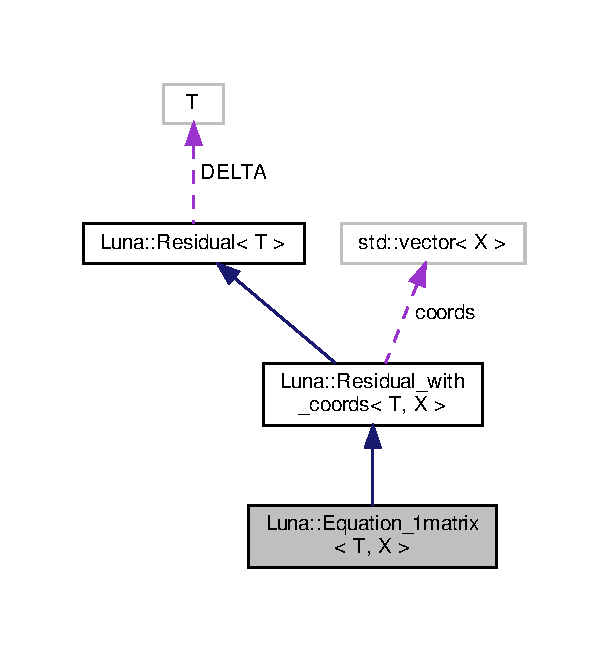
\includegraphics[width=292pt]{classLuna_1_1Equation__1matrix__coll__graph}
\end{center}
\end{figure}
\subsection*{Public Member Functions}
\begin{DoxyCompactItemize}
\item 
\hyperlink{classLuna_1_1Equation__1matrix_af76f7d2d3a138e8071390eb579fd2c4e}{Equation\+\_\+1matrix} (const unsigned \&order)
\begin{DoxyCompactList}\small\item\em Constructor. \end{DoxyCompactList}\item 
virtual \hyperlink{classLuna_1_1Equation__1matrix_a5f6241862fa31bb048be2e535df3eb94}{$\sim$\+Equation\+\_\+1matrix} ()
\begin{DoxyCompactList}\small\item\em Destructor. \end{DoxyCompactList}\item 
void \hyperlink{classLuna_1_1Equation__1matrix_a08f510d89ae39ed46752cddea5376ae8}{update} (const \hyperlink{classLuna_1_1Vector}{Vector}$<$ T $>$ \&\hyperlink{classLuna_1_1Residual_a41d9f863aa529f16c5d78fb19b4906bd}{state})
\begin{DoxyCompactList}\small\item\em Update the \hyperlink{classLuna_1_1Equation}{Equation} object for the current set of state variables. \end{DoxyCompactList}\item 
const \hyperlink{classLuna_1_1Matrix}{Matrix}$<$ T $>$ \& \hyperlink{classLuna_1_1Equation__1matrix_a7e0adf303491e67602d5e34ab7ec3ada}{matrix0} () const
\begin{DoxyCompactList}\small\item\em Return a handle to the matrix. \end{DoxyCompactList}\item 
virtual void \hyperlink{classLuna_1_1Equation__1matrix_ad2ddee223f6c9dfd0c95a867699bbd24}{get\+\_\+jacobian\+\_\+of\+\_\+matrix0\+\_\+mult\+\_\+vector} (const \hyperlink{classLuna_1_1Vector}{Vector}$<$ T $>$ \&\hyperlink{classLuna_1_1Residual_a41d9f863aa529f16c5d78fb19b4906bd}{state}, const \hyperlink{classLuna_1_1Vector}{Vector}$<$ T $>$ \&vec, \hyperlink{classLuna_1_1Matrix}{Matrix}$<$ T $>$ \&h) const
\begin{DoxyCompactList}\small\item\em Return the product of the Jacobian-\/of-\/the-\/matrix and a vector \textquotesingle{}vec\textquotesingle{} when the equation has a given \textquotesingle{}state\textquotesingle{}. \end{DoxyCompactList}\end{DoxyCompactItemize}
\subsection*{Protected Member Functions}
\begin{DoxyCompactItemize}
\item 
virtual void \hyperlink{classLuna_1_1Equation__1matrix_a2501535a6e92abc491bc491b3f64dc06}{matrix0} (const \hyperlink{classLuna_1_1Vector}{Vector}$<$ T $>$ \&x, \hyperlink{classLuna_1_1Matrix}{Matrix}$<$ T $>$ \&m) const
\begin{DoxyCompactList}\small\item\em Define the matrix in terms of the current state vector. \end{DoxyCompactList}\end{DoxyCompactItemize}
\subsection*{Additional Inherited Members}


\subsection{Detailed Description}
\subsubsection*{template$<$typename T, typename X = double$>$\newline
class Luna\+::\+Equation\+\_\+1matrix$<$ T, X $>$}



Definition at line 21 of file Equation\+\_\+1matrix.\+h.



\subsection{Constructor \& Destructor Documentation}
\mbox{\Hypertarget{classLuna_1_1Equation__1matrix_af76f7d2d3a138e8071390eb579fd2c4e}\label{classLuna_1_1Equation__1matrix_af76f7d2d3a138e8071390eb579fd2c4e}} 
\index{Luna\+::\+Equation\+\_\+1matrix@{Luna\+::\+Equation\+\_\+1matrix}!Equation\+\_\+1matrix@{Equation\+\_\+1matrix}}
\index{Equation\+\_\+1matrix@{Equation\+\_\+1matrix}!Luna\+::\+Equation\+\_\+1matrix@{Luna\+::\+Equation\+\_\+1matrix}}
\subsubsection{\texorpdfstring{Equation\+\_\+1matrix()}{Equation\_1matrix()}}
{\footnotesize\ttfamily template$<$typename T , typename X $>$ \\
\hyperlink{classLuna_1_1Equation__1matrix}{Luna\+::\+Equation\+\_\+1matrix}$<$ T, X $>$\+::\hyperlink{classLuna_1_1Equation__1matrix}{Equation\+\_\+1matrix} (\begin{DoxyParamCaption}\item[{const unsigned \&}]{order }\end{DoxyParamCaption})\hspace{0.3cm}{\ttfamily [explicit]}}



Constructor. 


\begin{DoxyParams}{Parameters}
{\em order} & The order of the system \\
\hline
\end{DoxyParams}


Definition at line 69 of file Equation\+\_\+1matrix.\+h.


\begin{DoxyCode}
69                                                                  :
70        Residual\_with\_coords<T, X>( order, 1 )
71  \{
72    \textcolor{keywordtype}{unsigned} sys\_order( \textcolor{keyword}{this} -> \hyperlink{classLuna_1_1Residual_a7facf1267eb277d84aeea8beba2cb200}{ORDER\_OF\_SYSTEM} );
73    MATRIX0\_AT\_LAST\_STATE = Matrix<T>( sys\_order, sys\_order, 0.0 );
74  \}
\end{DoxyCode}
\mbox{\Hypertarget{classLuna_1_1Equation__1matrix_a5f6241862fa31bb048be2e535df3eb94}\label{classLuna_1_1Equation__1matrix_a5f6241862fa31bb048be2e535df3eb94}} 
\index{Luna\+::\+Equation\+\_\+1matrix@{Luna\+::\+Equation\+\_\+1matrix}!````~Equation\+\_\+1matrix@{$\sim$\+Equation\+\_\+1matrix}}
\index{````~Equation\+\_\+1matrix@{$\sim$\+Equation\+\_\+1matrix}!Luna\+::\+Equation\+\_\+1matrix@{Luna\+::\+Equation\+\_\+1matrix}}
\subsubsection{\texorpdfstring{$\sim$\+Equation\+\_\+1matrix()}{~Equation\_1matrix()}}
{\footnotesize\ttfamily template$<$typename T , typename X $>$ \\
\hyperlink{classLuna_1_1Equation__1matrix}{Luna\+::\+Equation\+\_\+1matrix}$<$ T, X $>$\+::$\sim$\hyperlink{classLuna_1_1Equation__1matrix}{Equation\+\_\+1matrix} (\begin{DoxyParamCaption}{ }\end{DoxyParamCaption})\hspace{0.3cm}{\ttfamily [virtual]}}



Destructor. 



Definition at line 77 of file Equation\+\_\+1matrix.\+h.


\begin{DoxyCode}
78  \{\}
\end{DoxyCode}


\subsection{Member Function Documentation}
\mbox{\Hypertarget{classLuna_1_1Equation__1matrix_ad2ddee223f6c9dfd0c95a867699bbd24}\label{classLuna_1_1Equation__1matrix_ad2ddee223f6c9dfd0c95a867699bbd24}} 
\index{Luna\+::\+Equation\+\_\+1matrix@{Luna\+::\+Equation\+\_\+1matrix}!get\+\_\+jacobian\+\_\+of\+\_\+matrix0\+\_\+mult\+\_\+vector@{get\+\_\+jacobian\+\_\+of\+\_\+matrix0\+\_\+mult\+\_\+vector}}
\index{get\+\_\+jacobian\+\_\+of\+\_\+matrix0\+\_\+mult\+\_\+vector@{get\+\_\+jacobian\+\_\+of\+\_\+matrix0\+\_\+mult\+\_\+vector}!Luna\+::\+Equation\+\_\+1matrix@{Luna\+::\+Equation\+\_\+1matrix}}
\subsubsection{\texorpdfstring{get\+\_\+jacobian\+\_\+of\+\_\+matrix0\+\_\+mult\+\_\+vector()}{get\_jacobian\_of\_matrix0\_mult\_vector()}}
{\footnotesize\ttfamily template$<$typename T, typename X $>$ \\
void \hyperlink{classLuna_1_1Equation__1matrix}{Luna\+::\+Equation\+\_\+1matrix}$<$ T, X $>$\+::get\+\_\+jacobian\+\_\+of\+\_\+matrix0\+\_\+mult\+\_\+vector (\begin{DoxyParamCaption}\item[{const \hyperlink{classLuna_1_1Vector}{Vector}$<$ T $>$ \&}]{state,  }\item[{const \hyperlink{classLuna_1_1Vector}{Vector}$<$ T $>$ \&}]{vec,  }\item[{\hyperlink{classLuna_1_1Matrix}{Matrix}$<$ T $>$ \&}]{h }\end{DoxyParamCaption}) const\hspace{0.3cm}{\ttfamily [virtual]}}



Return the product of the Jacobian-\/of-\/the-\/matrix and a vector \textquotesingle{}vec\textquotesingle{} when the equation has a given \textquotesingle{}state\textquotesingle{}. 

The user should overload this if concerned about performance of the solver. If not overloaded, the default is to finite difference the Jacobian-\/of-\/the-\/matrix. 
\begin{DoxyParams}{Parameters}
{\em state} & The current state variables \\
\hline
{\em vec} & The vector which is multiplied by the Jacobian of the matrix \\
\hline
{\em h} & The resulting 2D matrix \\
\hline
\end{DoxyParams}


Definition at line 94 of file Equation\+\_\+1matrix.\+h.


\begin{DoxyCode}
96  \{
97    \textcolor{comment}{// We dont need state in the default implementation as its already been set}
98    \textcolor{comment}{// by the update method. You do need it for the user to overload this method}
99    \textcolor{comment}{// with an explicit analytical version however.}
100 
101    Vector<T> copy\_of\_state( \textcolor{keyword}{this} -> \hyperlink{classLuna_1_1Residual_abcfc99f00aa4cf3616b32dfd5315dece}{LAST\_STATE} );
102    Matrix<T> copy\_of\_matrix( MATRIX0\_AT\_LAST\_STATE );
103    std::vector< Matrix<T> > jacmatrix;
104    \textcolor{comment}{// update the Jacobian of the mass matrix}
105    \textcolor{keywordflow}{for} ( std::size\_t i = 0; i < \textcolor{keyword}{this} -> \hyperlink{classLuna_1_1Residual_a7facf1267eb277d84aeea8beba2cb200}{ORDER\_OF\_SYSTEM}; ++i )
106    \{
107      copy\_of\_state[ i ] += \textcolor{keyword}{this} -> \hyperlink{classLuna_1_1Residual_a1bf38ddfa149797de560dcb11c975fef}{DELTA};
108      \hyperlink{classLuna_1_1Equation__1matrix_a7e0adf303491e67602d5e34ab7ec3ada}{matrix0}( copy\_of\_state, copy\_of\_matrix );
109      copy\_of\_state[ i ] -= \textcolor{keyword}{this} -> \hyperlink{classLuna_1_1Residual_a1bf38ddfa149797de560dcb11c975fef}{DELTA};
110      copy\_of\_matrix -= MATRIX0\_AT\_LAST\_STATE;
111      copy\_of\_matrix *= ( 1. / \textcolor{keyword}{this} -> \hyperlink{classLuna_1_1Residual_a1bf38ddfa149797de560dcb11c975fef}{DELTA} );
112      \textcolor{comment}{// the 3D object that represents the Jacobian of the mass matrix}
113      jacmatrix.push\_back( copy\_of\_matrix );
114    \}
115    \textcolor{comment}{// evaluate the jacabian of mass contribution}
116    \textcolor{keywordflow}{for} ( \textcolor{keywordtype}{unsigned} i = 0; i < \textcolor{keyword}{this} -> \hyperlink{classLuna_1_1Residual_a7facf1267eb277d84aeea8beba2cb200}{ORDER\_OF\_SYSTEM}; ++i )
117    \{
118      \textcolor{keywordflow}{for} ( \textcolor{keywordtype}{unsigned} j = 0; j < \textcolor{keyword}{this} -> \hyperlink{classLuna_1_1Residual_a7facf1267eb277d84aeea8beba2cb200}{ORDER\_OF\_SYSTEM}; ++j )
119      \{
120        h( i, j ) = jacmatrix[ j ][ i ].dot( vec );
121      \}
122    \}
123  \}
\end{DoxyCode}
\mbox{\Hypertarget{classLuna_1_1Equation__1matrix_a7e0adf303491e67602d5e34ab7ec3ada}\label{classLuna_1_1Equation__1matrix_a7e0adf303491e67602d5e34ab7ec3ada}} 
\index{Luna\+::\+Equation\+\_\+1matrix@{Luna\+::\+Equation\+\_\+1matrix}!matrix0@{matrix0}}
\index{matrix0@{matrix0}!Luna\+::\+Equation\+\_\+1matrix@{Luna\+::\+Equation\+\_\+1matrix}}
\subsubsection{\texorpdfstring{matrix0()}{matrix0()}\hspace{0.1cm}{\footnotesize\ttfamily [1/2]}}
{\footnotesize\ttfamily template$<$typename T , typename X $>$ \\
const \hyperlink{classLuna_1_1Matrix}{Matrix}$<$ T $>$ \& \hyperlink{classLuna_1_1Equation__1matrix}{Luna\+::\+Equation\+\_\+1matrix}$<$ T, X $>$\+::matrix0 (\begin{DoxyParamCaption}{ }\end{DoxyParamCaption}) const\hspace{0.3cm}{\ttfamily [inline]}}



Return a handle to the matrix. 



Definition at line 88 of file Equation\+\_\+1matrix.\+h.


\begin{DoxyCode}
89  \{
90    \textcolor{keywordflow}{return} MATRIX0\_AT\_LAST\_STATE;
91  \}
\end{DoxyCode}
\mbox{\Hypertarget{classLuna_1_1Equation__1matrix_a2501535a6e92abc491bc491b3f64dc06}\label{classLuna_1_1Equation__1matrix_a2501535a6e92abc491bc491b3f64dc06}} 
\index{Luna\+::\+Equation\+\_\+1matrix@{Luna\+::\+Equation\+\_\+1matrix}!matrix0@{matrix0}}
\index{matrix0@{matrix0}!Luna\+::\+Equation\+\_\+1matrix@{Luna\+::\+Equation\+\_\+1matrix}}
\subsubsection{\texorpdfstring{matrix0()}{matrix0()}\hspace{0.1cm}{\footnotesize\ttfamily [2/2]}}
{\footnotesize\ttfamily template$<$typename T, typename X = double$>$ \\
virtual void \hyperlink{classLuna_1_1Equation__1matrix}{Luna\+::\+Equation\+\_\+1matrix}$<$ T, X $>$\+::matrix0 (\begin{DoxyParamCaption}\item[{const \hyperlink{classLuna_1_1Vector}{Vector}$<$ T $>$ \&}]{x,  }\item[{\hyperlink{classLuna_1_1Matrix}{Matrix}$<$ T $>$ \&}]{m }\end{DoxyParamCaption}) const\hspace{0.3cm}{\ttfamily [inline]}, {\ttfamily [protected]}, {\ttfamily [virtual]}}



Define the matrix in terms of the current state vector. 


\begin{DoxyParams}{Parameters}
{\em x} & The current state vector. \\
\hline
{\em m} & The matrix. \\
\hline
\end{DoxyParams}


Reimplemented in \hyperlink{classLuna_1_1nonlinear__equation_a467d48cbfdb69fddc877e00dc24a397a}{Luna\+::nonlinear\+\_\+equation}, and \hyperlink{classLuna_1_1test__equation_a955940cd7cc59fbaef213151075f1838}{Luna\+::test\+\_\+equation}.



Definition at line 54 of file Equation\+\_\+1matrix.\+h.


\begin{DoxyCode}
55    \{
56      std::string problem;
57      problem = \textcolor{stringliteral}{"The equation::matrix0 method has not been implemented!\(\backslash\)n"};
58      problem += \textcolor{stringliteral}{"You have to implement this method to define the equation.\(\backslash\)n"};
59      \textcolor{keywordflow}{throw} Error( problem );
60    \}
\end{DoxyCode}
\mbox{\Hypertarget{classLuna_1_1Equation__1matrix_a08f510d89ae39ed46752cddea5376ae8}\label{classLuna_1_1Equation__1matrix_a08f510d89ae39ed46752cddea5376ae8}} 
\index{Luna\+::\+Equation\+\_\+1matrix@{Luna\+::\+Equation\+\_\+1matrix}!update@{update}}
\index{update@{update}!Luna\+::\+Equation\+\_\+1matrix@{Luna\+::\+Equation\+\_\+1matrix}}
\subsubsection{\texorpdfstring{update()}{update()}}
{\footnotesize\ttfamily template$<$typename T, typename X $>$ \\
void \hyperlink{classLuna_1_1Equation__1matrix}{Luna\+::\+Equation\+\_\+1matrix}$<$ T, X $>$\+::update (\begin{DoxyParamCaption}\item[{const \hyperlink{classLuna_1_1Vector}{Vector}$<$ T $>$ \&}]{state }\end{DoxyParamCaption})}



Update the \hyperlink{classLuna_1_1Equation}{Equation} object for the current set of state variables. 


\begin{DoxyParams}{Parameters}
{\em state} & The state vector at which to set the equation object \\
\hline
\end{DoxyParams}


Definition at line 81 of file Equation\+\_\+1matrix.\+h.


\begin{DoxyCode}
82  \{
83      \hyperlink{classLuna_1_1Residual_ac1f39e77c729e6a4a1e10ac951f6c704}{Residual\_with\_coords<T, X>::update}( \hyperlink{classLuna_1_1Residual_a41d9f863aa529f16c5d78fb19b4906bd}{state} );
84      \hyperlink{classLuna_1_1Equation__1matrix_a7e0adf303491e67602d5e34ab7ec3ada}{matrix0}( \hyperlink{classLuna_1_1Residual_a41d9f863aa529f16c5d78fb19b4906bd}{state}, MATRIX0\_AT\_LAST\_STATE );
85  \}
\end{DoxyCode}


The documentation for this class was generated from the following file\+:\begin{DoxyCompactItemize}
\item 
include/\+Luna/\hyperlink{Equation__1matrix_8h}{Equation\+\_\+1matrix.\+h}\end{DoxyCompactItemize}

\hypertarget{classLuna_1_1Error}{}\section{Luna\+:\+:Error Class Reference}
\label{classLuna_1_1Error}\index{Luna\+::\+Error@{Luna\+::\+Error}}


A generic runtime error.  




{\ttfamily \#include $<$Error.\+h$>$}



Inheritance diagram for Luna\+:\+:Error\+:\nopagebreak
\begin{figure}[H]
\begin{center}
\leavevmode
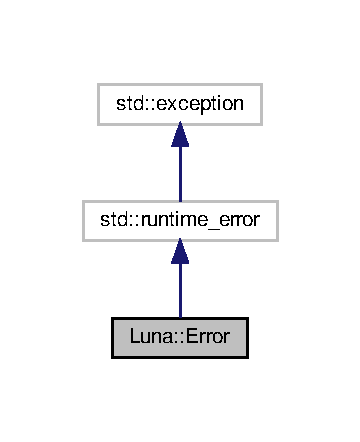
\includegraphics[width=173pt]{classLuna_1_1Error__inherit__graph}
\end{center}
\end{figure}


Collaboration diagram for Luna\+:\+:Error\+:\nopagebreak
\begin{figure}[H]
\begin{center}
\leavevmode
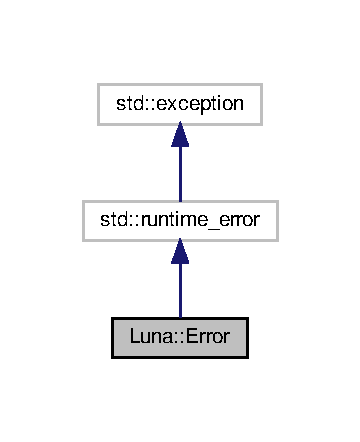
\includegraphics[width=173pt]{classLuna_1_1Error__coll__graph}
\end{center}
\end{figure}
\subsection*{Public Member Functions}
\begin{DoxyCompactItemize}
\item 
\hyperlink{classLuna_1_1Error_ab6532a3edbc267560cf74e02007e19b8}{Error} (const std\+::string \&problem)
\begin{DoxyCompactList}\small\item\em Constructor. \end{DoxyCompactList}\end{DoxyCompactItemize}


\subsection{Detailed Description}
A generic runtime error. 

Definition at line 15 of file Error.\+h.



\subsection{Constructor \& Destructor Documentation}
\mbox{\Hypertarget{classLuna_1_1Error_ab6532a3edbc267560cf74e02007e19b8}\label{classLuna_1_1Error_ab6532a3edbc267560cf74e02007e19b8}} 
\index{Luna\+::\+Error@{Luna\+::\+Error}!Error@{Error}}
\index{Error@{Error}!Luna\+::\+Error@{Luna\+::\+Error}}
\subsubsection{\texorpdfstring{Error()}{Error()}}
{\footnotesize\ttfamily Luna\+::\+Error\+::\+Error (\begin{DoxyParamCaption}\item[{const std\+::string \&}]{problem }\end{DoxyParamCaption})\hspace{0.3cm}{\ttfamily [inline]}}



Constructor. 


\begin{DoxyParams}{Parameters}
{\em problem} & \hyperlink{classLuna_1_1Error}{Error} string to be produced \\
\hline
\end{DoxyParams}


Definition at line 21 of file Error.\+h.


\begin{DoxyCode}
21                                       : std::runtime\_error( problem )
22     \{
23       error\_header();
24       std::cout << problem << std::endl;
25     \}
\end{DoxyCode}


The documentation for this class was generated from the following file\+:\begin{DoxyCompactItemize}
\item 
include/\+Luna/\hyperlink{Error_8h}{Error.\+h}\end{DoxyCompactItemize}

\hypertarget{classLuna_1_1left__BC}{}\section{Luna\+:\+:left\+\_\+\+BC Class Reference}
\label{classLuna_1_1left__BC}\index{Luna\+::left\+\_\+\+BC@{Luna\+::left\+\_\+\+BC}}


Inheritance diagram for Luna\+:\+:left\+\_\+\+BC\+:\nopagebreak
\begin{figure}[H]
\begin{center}
\leavevmode
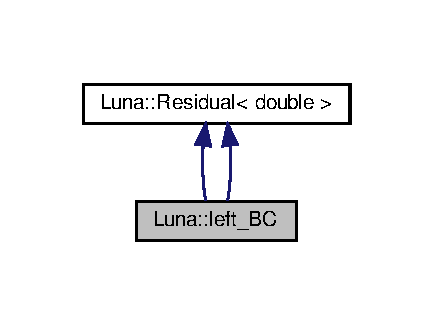
\includegraphics[width=208pt]{classLuna_1_1left__BC__inherit__graph}
\end{center}
\end{figure}


Collaboration diagram for Luna\+:\+:left\+\_\+\+BC\+:\nopagebreak
\begin{figure}[H]
\begin{center}
\leavevmode
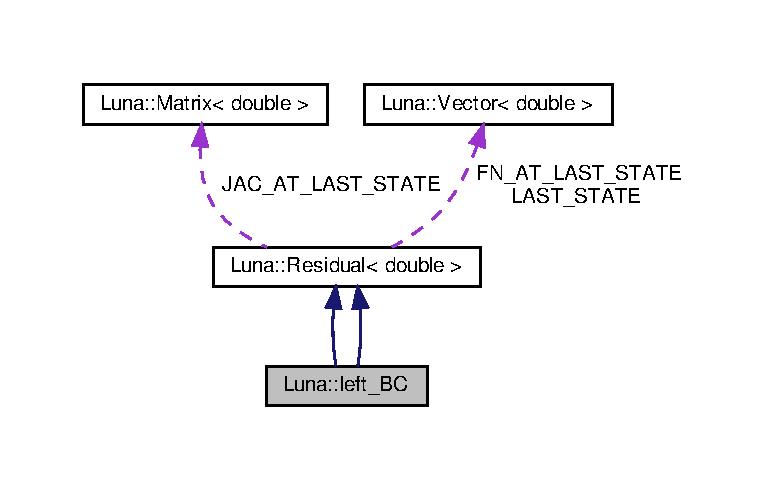
\includegraphics[width=350pt]{classLuna_1_1left__BC__coll__graph}
\end{center}
\end{figure}
\subsection*{Public Member Functions}
\begin{DoxyCompactItemize}
\item 
\hyperlink{classLuna_1_1left__BC_aad6be08c3e07998f09dd7d8ac1876e5c}{left\+\_\+\+BC} ()
\item 
void \hyperlink{classLuna_1_1left__BC_a01645de89a78c7c925d60bb68e994c90}{residual\+\_\+fn} (const \hyperlink{classLuna_1_1Vector}{Vector}$<$ double $>$ \&z, \hyperlink{classLuna_1_1Vector}{Vector}$<$ double $>$ \&B) const
\begin{DoxyCompactList}\small\item\em The residual function to be defined later. \end{DoxyCompactList}\item 
\hyperlink{classLuna_1_1left__BC_aad6be08c3e07998f09dd7d8ac1876e5c}{left\+\_\+\+BC} ()
\item 
void \hyperlink{classLuna_1_1left__BC_a01645de89a78c7c925d60bb68e994c90}{residual\+\_\+fn} (const \hyperlink{classLuna_1_1Vector}{Vector}$<$ double $>$ \&z, \hyperlink{classLuna_1_1Vector}{Vector}$<$ double $>$ \&B) const
\begin{DoxyCompactList}\small\item\em The residual function to be defined later. \end{DoxyCompactList}\end{DoxyCompactItemize}
\subsection*{Additional Inherited Members}


\subsection{Detailed Description}


Definition at line 42 of file Nonlinear\+\_\+\+O\+D\+E\+\_\+\+B\+V\+P.\+cpp.



\subsection{Constructor \& Destructor Documentation}
\mbox{\Hypertarget{classLuna_1_1left__BC_aad6be08c3e07998f09dd7d8ac1876e5c}\label{classLuna_1_1left__BC_aad6be08c3e07998f09dd7d8ac1876e5c}} 
\index{Luna\+::left\+\_\+\+BC@{Luna\+::left\+\_\+\+BC}!left\+\_\+\+BC@{left\+\_\+\+BC}}
\index{left\+\_\+\+BC@{left\+\_\+\+BC}!Luna\+::left\+\_\+\+BC@{Luna\+::left\+\_\+\+BC}}
\subsubsection{\texorpdfstring{left\+\_\+\+B\+C()}{left\_BC()}\hspace{0.1cm}{\footnotesize\ttfamily [1/2]}}
{\footnotesize\ttfamily Luna\+::left\+\_\+\+B\+C\+::left\+\_\+\+BC (\begin{DoxyParamCaption}{ }\end{DoxyParamCaption})\hspace{0.3cm}{\ttfamily [inline]}}



Definition at line 46 of file Nonlinear\+\_\+\+O\+D\+E\+\_\+\+B\+V\+P.\+cpp.


\begin{DoxyCode}
46 : \hyperlink{classLuna_1_1Residual}{Residual<double>} ( 1, 2 ) \{\}
\end{DoxyCode}
\mbox{\Hypertarget{classLuna_1_1left__BC_aad6be08c3e07998f09dd7d8ac1876e5c}\label{classLuna_1_1left__BC_aad6be08c3e07998f09dd7d8ac1876e5c}} 
\index{Luna\+::left\+\_\+\+BC@{Luna\+::left\+\_\+\+BC}!left\+\_\+\+BC@{left\+\_\+\+BC}}
\index{left\+\_\+\+BC@{left\+\_\+\+BC}!Luna\+::left\+\_\+\+BC@{Luna\+::left\+\_\+\+BC}}
\subsubsection{\texorpdfstring{left\+\_\+\+B\+C()}{left\_BC()}\hspace{0.1cm}{\footnotesize\ttfamily [2/2]}}
{\footnotesize\ttfamily Luna\+::left\+\_\+\+B\+C\+::left\+\_\+\+BC (\begin{DoxyParamCaption}{ }\end{DoxyParamCaption})\hspace{0.3cm}{\ttfamily [inline]}}



Definition at line 38 of file O\+D\+E\+\_\+\+B\+V\+P\+\_\+test.\+cpp.


\begin{DoxyCode}
38 : \hyperlink{classLuna_1_1Residual}{Residual<double>} ( 1, 2 ) \{\}
\end{DoxyCode}


\subsection{Member Function Documentation}
\mbox{\Hypertarget{classLuna_1_1left__BC_a01645de89a78c7c925d60bb68e994c90}\label{classLuna_1_1left__BC_a01645de89a78c7c925d60bb68e994c90}} 
\index{Luna\+::left\+\_\+\+BC@{Luna\+::left\+\_\+\+BC}!residual\+\_\+fn@{residual\+\_\+fn}}
\index{residual\+\_\+fn@{residual\+\_\+fn}!Luna\+::left\+\_\+\+BC@{Luna\+::left\+\_\+\+BC}}
\subsubsection{\texorpdfstring{residual\+\_\+fn()}{residual\_fn()}\hspace{0.1cm}{\footnotesize\ttfamily [1/2]}}
{\footnotesize\ttfamily void Luna\+::left\+\_\+\+B\+C\+::residual\+\_\+fn (\begin{DoxyParamCaption}\item[{const \hyperlink{classLuna_1_1Vector}{Vector}$<$ double $>$ \&}]{state,  }\item[{\hyperlink{classLuna_1_1Vector}{Vector}$<$ double $>$ \&}]{f }\end{DoxyParamCaption}) const\hspace{0.3cm}{\ttfamily [inline]}, {\ttfamily [virtual]}}



The residual function to be defined later. 


\begin{DoxyParams}{Parameters}
{\em state} & The current state \hyperlink{classLuna_1_1Vector}{Vector} \\
\hline
{\em f} & The function \hyperlink{classLuna_1_1Vector}{Vector} to be updated \\
\hline
\end{DoxyParams}


Reimplemented from \hyperlink{classLuna_1_1Residual_ae1b1ebe3314c788b176bcac7b328de5c}{Luna\+::\+Residual$<$ double $>$}.



Definition at line 40 of file O\+D\+E\+\_\+\+B\+V\+P\+\_\+test.\+cpp.



References y.


\begin{DoxyCode}
41         \{
42             B[ 0 ] = z[ \hyperlink{ODE__BVP__test_8cpp_adf764cbdea00d65edcd07bb9953ad2b7ae1f9fdb8b786c63efc4ce44eeacd17f2}{y} ] + 2.0;
43         \}
\end{DoxyCode}
\mbox{\Hypertarget{classLuna_1_1left__BC_a01645de89a78c7c925d60bb68e994c90}\label{classLuna_1_1left__BC_a01645de89a78c7c925d60bb68e994c90}} 
\index{Luna\+::left\+\_\+\+BC@{Luna\+::left\+\_\+\+BC}!residual\+\_\+fn@{residual\+\_\+fn}}
\index{residual\+\_\+fn@{residual\+\_\+fn}!Luna\+::left\+\_\+\+BC@{Luna\+::left\+\_\+\+BC}}
\subsubsection{\texorpdfstring{residual\+\_\+fn()}{residual\_fn()}\hspace{0.1cm}{\footnotesize\ttfamily [2/2]}}
{\footnotesize\ttfamily void Luna\+::left\+\_\+\+B\+C\+::residual\+\_\+fn (\begin{DoxyParamCaption}\item[{const \hyperlink{classLuna_1_1Vector}{Vector}$<$ double $>$ \&}]{state,  }\item[{\hyperlink{classLuna_1_1Vector}{Vector}$<$ double $>$ \&}]{f }\end{DoxyParamCaption}) const\hspace{0.3cm}{\ttfamily [inline]}, {\ttfamily [virtual]}}



The residual function to be defined later. 


\begin{DoxyParams}{Parameters}
{\em state} & The current state \hyperlink{classLuna_1_1Vector}{Vector} \\
\hline
{\em f} & The function \hyperlink{classLuna_1_1Vector}{Vector} to be updated \\
\hline
\end{DoxyParams}


Reimplemented from \hyperlink{classLuna_1_1Residual_ae1b1ebe3314c788b176bcac7b328de5c}{Luna\+::\+Residual$<$ double $>$}.



Definition at line 48 of file Nonlinear\+\_\+\+O\+D\+E\+\_\+\+B\+V\+P.\+cpp.



References f.


\begin{DoxyCode}
49         \{
50             B[ 0 ] = z[ \hyperlink{Nonlinear__ODE__BVP_8cpp_a06fc87d81c62e9abb8790b6e5713c55ba7ce756344023b99e5ab27b804feb765c}{f} ] - 2.0;
51         \}
\end{DoxyCode}


The documentation for this class was generated from the following files\+:\begin{DoxyCompactItemize}
\item 
Examples/\hyperlink{Nonlinear__ODE__BVP_8cpp}{Nonlinear\+\_\+\+O\+D\+E\+\_\+\+B\+V\+P.\+cpp}\item 
Examples/\hyperlink{ODE__BVP__test_8cpp}{O\+D\+E\+\_\+\+B\+V\+P\+\_\+test.\+cpp}\end{DoxyCompactItemize}

\hypertarget{classLuna_1_1LinearEigensystem}{}\section{Luna\+:\+:Linear\+Eigensystem$<$ T $>$ Class Template Reference}
\label{classLuna_1_1LinearEigensystem}\index{Luna\+::\+Linear\+Eigensystem$<$ T $>$@{Luna\+::\+Linear\+Eigensystem$<$ T $>$}}


A \hyperlink{classLuna_1_1LinearEigensystem}{Linear\+Eigensystem} class for use with double and std\+::complex$<$double$>$  




{\ttfamily \#include $<$Linear\+Eigensystem.\+h$>$}

\subsection*{Public Member Functions}
\begin{DoxyCompactItemize}
\item 
\hyperlink{classLuna_1_1LinearEigensystem_a6a285716463cb439b2c82d0055d247c5}{Linear\+Eigensystem} ()
\begin{DoxyCompactList}\small\item\em Constructor for a \hyperlink{classLuna_1_1LinearEigensystem}{Linear\+Eigensystem}. \end{DoxyCompactList}\item 
\hyperlink{classLuna_1_1LinearEigensystem_a3bb8fffcca088facf2e8efedc20d9944}{$\sim$\+Linear\+Eigensystem} ()
\begin{DoxyCompactList}\small\item\em Destructor. \end{DoxyCompactList}\item 
void \hyperlink{classLuna_1_1LinearEigensystem_ae109e1012fda347ac9c1da4fa30313f6}{compute\+\_\+real\+\_\+symmetric} (const \hyperlink{classLuna_1_1Matrix}{Matrix}$<$ double $>$ \&a, bool compute\+\_\+evecs=true)
\begin{DoxyCompactList}\small\item\em Solve a \hyperlink{classLuna_1_1LinearEigensystem}{Linear\+Eigensystem} A$\ast$v=lambda$\ast$v where A is a real symmetric \hyperlink{classLuna_1_1Matrix}{Matrix} to give the eigenvalues ( and optionally the eigenvectors ) \end{DoxyCompactList}\item 
void \hyperlink{classLuna_1_1LinearEigensystem_a91ac311c3fe4226c4652b6bf41fc0d91}{compute\+\_\+real\+\_\+symmetric\+\_\+tridiagonal} (const \hyperlink{classLuna_1_1Vector}{Vector}$<$ double $>$ \&diag, const \hyperlink{classLuna_1_1Vector}{Vector}$<$ double $>$ \&off\+\_\+diag, bool compute\+\_\+evecs=true)
\begin{DoxyCompactList}\small\item\em Solve a \hyperlink{classLuna_1_1LinearEigensystem}{Linear\+Eigensystem} A$\ast$v=lambda$\ast$v where A is a real symmetric tridiagonal \hyperlink{classLuna_1_1Matrix}{Matrix} to give the eigenvalues ( and optionally the eigenvectors ) \end{DoxyCompactList}\item 
void \hyperlink{classLuna_1_1LinearEigensystem_ab303a80cc2cf6bfe232b9d62efe13109}{compute\+\_\+real} (const \hyperlink{classLuna_1_1Matrix}{Matrix}$<$ double $>$ \&a, bool compute\+\_\+evecs=true)
\begin{DoxyCompactList}\small\item\em Solve a \hyperlink{classLuna_1_1LinearEigensystem}{Linear\+Eigensystem} A$\ast$v=lambda$\ast$v where A is a real \hyperlink{classLuna_1_1Matrix}{Matrix} to give the eigenvalues ( and optionally the eigenvectors ) \end{DoxyCompactList}\item 
\hyperlink{classLuna_1_1Vector}{Vector}$<$ std\+::complex$<$ double $>$ $>$ \hyperlink{classLuna_1_1LinearEigensystem_ad74f60a4830eefb2858ab92765dc0ae4}{eigenvalues} () const
\begin{DoxyCompactList}\small\item\em Return the eigenvalues. \end{DoxyCompactList}\item 
\hyperlink{classLuna_1_1Matrix}{Matrix}$<$ T $>$ \hyperlink{classLuna_1_1LinearEigensystem_ab68a36f7f1c1ecf9da83df84be6e49e9}{eigenvector\+\_\+matrix} () const
\begin{DoxyCompactList}\small\item\em Return a \hyperlink{classLuna_1_1Matrix}{Matrix} containing the eigenvectors. \end{DoxyCompactList}\item 
std\+::vector$<$ \hyperlink{classLuna_1_1Vector}{Vector}$<$ std\+::complex$<$ double $>$ $>$ $>$ \hyperlink{classLuna_1_1LinearEigensystem_a34fd0e8eef6dc0e85a13d1cb78beb32f}{eigenvectors} () const
\begin{DoxyCompactList}\small\item\em Return an std\+::vector of eigenvectors. \end{DoxyCompactList}\item 
{\footnotesize template$<$$>$ }\\void \hyperlink{classLuna_1_1LinearEigensystem_a239e3ff62330c51c94d0112de0318249}{compute\+\_\+real\+\_\+symmetric} (const \hyperlink{classLuna_1_1Matrix}{Matrix}$<$ double $>$ \&a, bool compute\+\_\+evecs)
\item 
{\footnotesize template$<$$>$ }\\void \hyperlink{classLuna_1_1LinearEigensystem_a080e0fe1d3baa1f6c5b56b9ae8082ae6}{compute\+\_\+real\+\_\+symmetric\+\_\+tridiagonal} (const \hyperlink{classLuna_1_1Vector}{Vector}$<$ double $>$ \&diag, const \hyperlink{classLuna_1_1Vector}{Vector}$<$ double $>$ \&off\+\_\+diag, bool compute\+\_\+evecs)
\item 
{\footnotesize template$<$$>$ }\\void \hyperlink{classLuna_1_1LinearEigensystem_a0aa01a39e1b44cc2cf225c8566d6bd95}{compute\+\_\+real} (const \hyperlink{classLuna_1_1Matrix}{Matrix}$<$ double $>$ \&a, bool compute\+\_\+evecs)
\end{DoxyCompactItemize}


\subsection{Detailed Description}
\subsubsection*{template$<$class T$>$\newline
class Luna\+::\+Linear\+Eigensystem$<$ T $>$}

A \hyperlink{classLuna_1_1LinearEigensystem}{Linear\+Eigensystem} class for use with double and std\+::complex$<$double$>$ 

Definition at line 25 of file Linear\+Eigensystem.\+h.



\subsection{Constructor \& Destructor Documentation}
\mbox{\Hypertarget{classLuna_1_1LinearEigensystem_a6a285716463cb439b2c82d0055d247c5}\label{classLuna_1_1LinearEigensystem_a6a285716463cb439b2c82d0055d247c5}} 
\index{Luna\+::\+Linear\+Eigensystem@{Luna\+::\+Linear\+Eigensystem}!Linear\+Eigensystem@{Linear\+Eigensystem}}
\index{Linear\+Eigensystem@{Linear\+Eigensystem}!Luna\+::\+Linear\+Eigensystem@{Luna\+::\+Linear\+Eigensystem}}
\subsubsection{\texorpdfstring{Linear\+Eigensystem()}{LinearEigensystem()}}
{\footnotesize\ttfamily template$<$class T$>$ \\
\hyperlink{classLuna_1_1LinearEigensystem}{Luna\+::\+Linear\+Eigensystem}$<$ T $>$\+::\hyperlink{classLuna_1_1LinearEigensystem}{Linear\+Eigensystem} (\begin{DoxyParamCaption}{ }\end{DoxyParamCaption})\hspace{0.3cm}{\ttfamily [inline]}}



Constructor for a \hyperlink{classLuna_1_1LinearEigensystem}{Linear\+Eigensystem}. 



Definition at line 45 of file Linear\+Eigensystem.\+h.


\begin{DoxyCode}
45                         : EIGENVALUES\_COMPUTED( \textcolor{keyword}{false} ),
46                           EIGENVECTORS\_COMPUTED( \textcolor{keyword}{false} )
47     \{\}
\end{DoxyCode}
\mbox{\Hypertarget{classLuna_1_1LinearEigensystem_a3bb8fffcca088facf2e8efedc20d9944}\label{classLuna_1_1LinearEigensystem_a3bb8fffcca088facf2e8efedc20d9944}} 
\index{Luna\+::\+Linear\+Eigensystem@{Luna\+::\+Linear\+Eigensystem}!````~Linear\+Eigensystem@{$\sim$\+Linear\+Eigensystem}}
\index{````~Linear\+Eigensystem@{$\sim$\+Linear\+Eigensystem}!Luna\+::\+Linear\+Eigensystem@{Luna\+::\+Linear\+Eigensystem}}
\subsubsection{\texorpdfstring{$\sim$\+Linear\+Eigensystem()}{~LinearEigensystem()}}
{\footnotesize\ttfamily template$<$class T$>$ \\
\hyperlink{classLuna_1_1LinearEigensystem}{Luna\+::\+Linear\+Eigensystem}$<$ T $>$\+::$\sim$\hyperlink{classLuna_1_1LinearEigensystem}{Linear\+Eigensystem} (\begin{DoxyParamCaption}{ }\end{DoxyParamCaption})\hspace{0.3cm}{\ttfamily [inline]}}



Destructor. 



Definition at line 50 of file Linear\+Eigensystem.\+h.



References Luna\+::\+Linear\+Eigensystem$<$ T $>$\+::compute\+\_\+real(), Luna\+::\+Linear\+Eigensystem$<$ T $>$\+::compute\+\_\+real\+\_\+symmetric(), Luna\+::\+Linear\+Eigensystem$<$ T $>$\+::compute\+\_\+real\+\_\+symmetric\+\_\+tridiagonal(), Luna\+::\+Linear\+Eigensystem$<$ T $>$\+::eigenvalues(), Luna\+::\+Linear\+Eigensystem$<$ T $>$\+::eigenvector\+\_\+matrix(), Luna\+::\+Linear\+Eigensystem$<$ T $>$\+::eigenvectors(), Heat\+\_\+plot\+::t, Heat\+\_\+plot\+::u, Heat\+\_\+plot\+::x, and y.


\begin{DoxyCode}
50 \{\}
\end{DoxyCode}


\subsection{Member Function Documentation}
\mbox{\Hypertarget{classLuna_1_1LinearEigensystem_ab303a80cc2cf6bfe232b9d62efe13109}\label{classLuna_1_1LinearEigensystem_ab303a80cc2cf6bfe232b9d62efe13109}} 
\index{Luna\+::\+Linear\+Eigensystem@{Luna\+::\+Linear\+Eigensystem}!compute\+\_\+real@{compute\+\_\+real}}
\index{compute\+\_\+real@{compute\+\_\+real}!Luna\+::\+Linear\+Eigensystem@{Luna\+::\+Linear\+Eigensystem}}
\subsubsection{\texorpdfstring{compute\+\_\+real()}{compute\_real()}\hspace{0.1cm}{\footnotesize\ttfamily [1/2]}}
{\footnotesize\ttfamily template$<$class T$>$ \\
void \hyperlink{classLuna_1_1LinearEigensystem}{Luna\+::\+Linear\+Eigensystem}$<$ T $>$\+::compute\+\_\+real (\begin{DoxyParamCaption}\item[{const \hyperlink{classLuna_1_1Matrix}{Matrix}$<$ double $>$ \&}]{a,  }\item[{bool}]{compute\+\_\+evecs = {\ttfamily true} }\end{DoxyParamCaption})}



Solve a \hyperlink{classLuna_1_1LinearEigensystem}{Linear\+Eigensystem} A$\ast$v=lambda$\ast$v where A is a real \hyperlink{classLuna_1_1Matrix}{Matrix} to give the eigenvalues ( and optionally the eigenvectors ) 


\begin{DoxyParams}{Parameters}
{\em a} & The \hyperlink{classLuna_1_1Matrix}{Matrix} A in the eigensystem \\
\hline
{\em compute\+\_\+evecs} & True if the eigenvectors are to be computed too \\
\hline
\end{DoxyParams}


Referenced by main(), and Luna\+::\+Linear\+Eigensystem$<$ T $>$\+::$\sim$\+Linear\+Eigensystem().

\mbox{\Hypertarget{classLuna_1_1LinearEigensystem_a0aa01a39e1b44cc2cf225c8566d6bd95}\label{classLuna_1_1LinearEigensystem_a0aa01a39e1b44cc2cf225c8566d6bd95}} 
\index{Luna\+::\+Linear\+Eigensystem@{Luna\+::\+Linear\+Eigensystem}!compute\+\_\+real@{compute\+\_\+real}}
\index{compute\+\_\+real@{compute\+\_\+real}!Luna\+::\+Linear\+Eigensystem@{Luna\+::\+Linear\+Eigensystem}}
\subsubsection{\texorpdfstring{compute\+\_\+real()}{compute\_real()}\hspace{0.1cm}{\footnotesize\ttfamily [2/2]}}
{\footnotesize\ttfamily template$<$$>$ \\
void \hyperlink{classLuna_1_1LinearEigensystem}{Luna\+::\+Linear\+Eigensystem}$<$ double $>$\+::compute\+\_\+real (\begin{DoxyParamCaption}\item[{const \hyperlink{classLuna_1_1Matrix}{Matrix}$<$ double $>$ \&}]{a,  }\item[{bool}]{compute\+\_\+evecs }\end{DoxyParamCaption})\hspace{0.3cm}{\ttfamily [inline]}}



Definition at line 334 of file Linear\+Eigensystem.\+h.



References Luna\+::\+Matrix$<$ T $>$\+::cols(), and Luna\+::\+Matrix$<$ T $>$\+::rows().


\begin{DoxyCode}
336   \{
337     \textcolor{keywordflow}{if} ( a.\hyperlink{classLuna_1_1Matrix_ae7b0b30c3e22ba252d660f093757295e}{rows}() != a.\hyperlink{classLuna_1_1Matrix_aa7472f90f4c470535e722f3a389a19b1}{cols}() )
338     \{
339       \textcolor{keywordflow}{throw} Error( \textcolor{stringliteral}{"compute\_real error: Matrix is not square."});
340     \}
341     A = a;
342     \hyperlink{namespaceHeat__plot_a7d050092798e28458a263710837bda77}{N} = a.\hyperlink{classLuna_1_1Matrix_ae7b0b30c3e22ba252d660f093757295e}{rows}();
343     balance();
344     elmhes();
345     \textcolor{keywordflow}{if} ( compute\_evecs ) \{
346       EIGENVECTORS.resize( \hyperlink{namespaceHeat__plot_a7d050092798e28458a263710837bda77}{N}, \hyperlink{namespaceHeat__plot_a7d050092798e28458a263710837bda77}{N} );
347       EIGENVECTORS.fill( 1.0 );
348       eltran();
349       hqr2();
350       balbak();
351       sortvecs();
352       EIGENVALUES\_COMPUTED = \textcolor{keyword}{true};
353       EIGENVECTORS\_COMPUTED = \textcolor{keyword}{true};
354     \} \textcolor{keywordflow}{else} \{
355       hqr();
356       sort\_unsymm();
357       EIGENVALUES\_COMPUTED = \textcolor{keyword}{true};
358     \}
359   \}
\end{DoxyCode}
\mbox{\Hypertarget{classLuna_1_1LinearEigensystem_ae109e1012fda347ac9c1da4fa30313f6}\label{classLuna_1_1LinearEigensystem_ae109e1012fda347ac9c1da4fa30313f6}} 
\index{Luna\+::\+Linear\+Eigensystem@{Luna\+::\+Linear\+Eigensystem}!compute\+\_\+real\+\_\+symmetric@{compute\+\_\+real\+\_\+symmetric}}
\index{compute\+\_\+real\+\_\+symmetric@{compute\+\_\+real\+\_\+symmetric}!Luna\+::\+Linear\+Eigensystem@{Luna\+::\+Linear\+Eigensystem}}
\subsubsection{\texorpdfstring{compute\+\_\+real\+\_\+symmetric()}{compute\_real\_symmetric()}\hspace{0.1cm}{\footnotesize\ttfamily [1/2]}}
{\footnotesize\ttfamily template$<$class T$>$ \\
void \hyperlink{classLuna_1_1LinearEigensystem}{Luna\+::\+Linear\+Eigensystem}$<$ T $>$\+::compute\+\_\+real\+\_\+symmetric (\begin{DoxyParamCaption}\item[{const \hyperlink{classLuna_1_1Matrix}{Matrix}$<$ double $>$ \&}]{a,  }\item[{bool}]{compute\+\_\+evecs = {\ttfamily true} }\end{DoxyParamCaption})}



Solve a \hyperlink{classLuna_1_1LinearEigensystem}{Linear\+Eigensystem} A$\ast$v=lambda$\ast$v where A is a real symmetric \hyperlink{classLuna_1_1Matrix}{Matrix} to give the eigenvalues ( and optionally the eigenvectors ) 


\begin{DoxyParams}{Parameters}
{\em a} & The \hyperlink{classLuna_1_1Matrix}{Matrix} A in the eigensystem \\
\hline
{\em compute\+\_\+evecs} & True if the eigenvectors are to be computed \\
\hline
\end{DoxyParams}


Referenced by main(), and Luna\+::\+Linear\+Eigensystem$<$ T $>$\+::$\sim$\+Linear\+Eigensystem().

\mbox{\Hypertarget{classLuna_1_1LinearEigensystem_a239e3ff62330c51c94d0112de0318249}\label{classLuna_1_1LinearEigensystem_a239e3ff62330c51c94d0112de0318249}} 
\index{Luna\+::\+Linear\+Eigensystem@{Luna\+::\+Linear\+Eigensystem}!compute\+\_\+real\+\_\+symmetric@{compute\+\_\+real\+\_\+symmetric}}
\index{compute\+\_\+real\+\_\+symmetric@{compute\+\_\+real\+\_\+symmetric}!Luna\+::\+Linear\+Eigensystem@{Luna\+::\+Linear\+Eigensystem}}
\subsubsection{\texorpdfstring{compute\+\_\+real\+\_\+symmetric()}{compute\_real\_symmetric()}\hspace{0.1cm}{\footnotesize\ttfamily [2/2]}}
{\footnotesize\ttfamily template$<$$>$ \\
void \hyperlink{classLuna_1_1LinearEigensystem}{Luna\+::\+Linear\+Eigensystem}$<$ double $>$\+::compute\+\_\+real\+\_\+symmetric (\begin{DoxyParamCaption}\item[{const \hyperlink{classLuna_1_1Matrix}{Matrix}$<$ double $>$ \&}]{a,  }\item[{bool}]{compute\+\_\+evecs }\end{DoxyParamCaption})\hspace{0.3cm}{\ttfamily [inline]}}



Definition at line 270 of file Linear\+Eigensystem.\+h.



References Luna\+::\+Matrix$<$ T $>$\+::cols(), Luna\+::\+Vector$<$ T $>$\+::resize(), and Luna\+::\+Matrix$<$ T $>$\+::rows().


\begin{DoxyCode}
272   \{
273     \textcolor{keywordflow}{if} ( a.\hyperlink{classLuna_1_1Matrix_ae7b0b30c3e22ba252d660f093757295e}{rows}() != a.\hyperlink{classLuna_1_1Matrix_aa7472f90f4c470535e722f3a389a19b1}{cols}() )
274     \{
275       \textcolor{keywordflow}{throw} Error( \textcolor{stringliteral}{"compute\_real\_symmetric error: Matrix is not square."});
276     \}
277     Matrix<double> z( a );
278     Vector<double> diag, off\_diag;
279     tred2( z, diag, off\_diag, compute\_evecs );
280     tqli( z, diag, off\_diag, compute\_evecs );
281     sort( diag, z, compute\_evecs );
282 
283     std::size\_t n( z.rows() );
284     EIGENVALUES.\hyperlink{classLuna_1_1Vector_ae1394f960d5cac3e60f6b1561f38e453}{resize}( n );
285     EIGENVECTORS.resize( n, n );
286     \textcolor{keywordflow}{for} ( std::size\_t i = 0; i < n; i++ )
287     \{
288       EIGENVALUES[ i ] = diag[ i ];
289     \}
290     EIGENVALUES\_COMPUTED = \textcolor{keyword}{true};
291     \textcolor{keywordflow}{if} ( compute\_evecs )
292     \{
293       EIGENVECTORS = z;
294       EIGENVECTORS\_COMPUTED = \textcolor{keyword}{true};
295     \}
296   \}
\end{DoxyCode}
\mbox{\Hypertarget{classLuna_1_1LinearEigensystem_a91ac311c3fe4226c4652b6bf41fc0d91}\label{classLuna_1_1LinearEigensystem_a91ac311c3fe4226c4652b6bf41fc0d91}} 
\index{Luna\+::\+Linear\+Eigensystem@{Luna\+::\+Linear\+Eigensystem}!compute\+\_\+real\+\_\+symmetric\+\_\+tridiagonal@{compute\+\_\+real\+\_\+symmetric\+\_\+tridiagonal}}
\index{compute\+\_\+real\+\_\+symmetric\+\_\+tridiagonal@{compute\+\_\+real\+\_\+symmetric\+\_\+tridiagonal}!Luna\+::\+Linear\+Eigensystem@{Luna\+::\+Linear\+Eigensystem}}
\subsubsection{\texorpdfstring{compute\+\_\+real\+\_\+symmetric\+\_\+tridiagonal()}{compute\_real\_symmetric\_tridiagonal()}\hspace{0.1cm}{\footnotesize\ttfamily [1/2]}}
{\footnotesize\ttfamily template$<$class T$>$ \\
void \hyperlink{classLuna_1_1LinearEigensystem}{Luna\+::\+Linear\+Eigensystem}$<$ T $>$\+::compute\+\_\+real\+\_\+symmetric\+\_\+tridiagonal (\begin{DoxyParamCaption}\item[{const \hyperlink{classLuna_1_1Vector}{Vector}$<$ double $>$ \&}]{diag,  }\item[{const \hyperlink{classLuna_1_1Vector}{Vector}$<$ double $>$ \&}]{off\+\_\+diag,  }\item[{bool}]{compute\+\_\+evecs = {\ttfamily true} }\end{DoxyParamCaption})}



Solve a \hyperlink{classLuna_1_1LinearEigensystem}{Linear\+Eigensystem} A$\ast$v=lambda$\ast$v where A is a real symmetric tridiagonal \hyperlink{classLuna_1_1Matrix}{Matrix} to give the eigenvalues ( and optionally the eigenvectors ) 


\begin{DoxyParams}{Parameters}
{\em diag} & The \hyperlink{classLuna_1_1Vector}{Vector} of main diagonal entries in the A \hyperlink{classLuna_1_1Matrix}{Matrix} \\
\hline
{\em off\+\_\+diag} & The \hyperlink{classLuna_1_1Vector}{Vector} of off-\/diagonal entries in the A \hyperlink{classLuna_1_1Matrix}{Matrix} \\
\hline
{\em compute\+\_\+evecs} & True if the eigenvectors are to be computed \\
\hline
\end{DoxyParams}


Referenced by main(), and Luna\+::\+Linear\+Eigensystem$<$ T $>$\+::$\sim$\+Linear\+Eigensystem().

\mbox{\Hypertarget{classLuna_1_1LinearEigensystem_a080e0fe1d3baa1f6c5b56b9ae8082ae6}\label{classLuna_1_1LinearEigensystem_a080e0fe1d3baa1f6c5b56b9ae8082ae6}} 
\index{Luna\+::\+Linear\+Eigensystem@{Luna\+::\+Linear\+Eigensystem}!compute\+\_\+real\+\_\+symmetric\+\_\+tridiagonal@{compute\+\_\+real\+\_\+symmetric\+\_\+tridiagonal}}
\index{compute\+\_\+real\+\_\+symmetric\+\_\+tridiagonal@{compute\+\_\+real\+\_\+symmetric\+\_\+tridiagonal}!Luna\+::\+Linear\+Eigensystem@{Luna\+::\+Linear\+Eigensystem}}
\subsubsection{\texorpdfstring{compute\+\_\+real\+\_\+symmetric\+\_\+tridiagonal()}{compute\_real\_symmetric\_tridiagonal()}\hspace{0.1cm}{\footnotesize\ttfamily [2/2]}}
{\footnotesize\ttfamily template$<$$>$ \\
void \hyperlink{classLuna_1_1LinearEigensystem}{Luna\+::\+Linear\+Eigensystem}$<$ double $>$\+::compute\+\_\+real\+\_\+symmetric\+\_\+tridiagonal (\begin{DoxyParamCaption}\item[{const \hyperlink{classLuna_1_1Vector}{Vector}$<$ double $>$ \&}]{diag,  }\item[{const \hyperlink{classLuna_1_1Vector}{Vector}$<$ double $>$ \&}]{off\+\_\+diag,  }\item[{bool}]{compute\+\_\+evecs }\end{DoxyParamCaption})\hspace{0.3cm}{\ttfamily [inline]}}



Definition at line 299 of file Linear\+Eigensystem.\+h.



References Luna\+::\+Vector$<$ T $>$\+::push\+\_\+front(), Luna\+::\+Vector$<$ T $>$\+::resize(), and Luna\+::\+Vector$<$ T $>$\+::size().


\begin{DoxyCode}
302   \{
303     \textcolor{keywordflow}{if} ( diag.\hyperlink{classLuna_1_1Vector_ac9b6ed7a0df401728f27c193fbc8f4d8}{size}() != off\_diag.\hyperlink{classLuna_1_1Vector_ac9b6ed7a0df401728f27c193fbc8f4d8}{size}() + 1 )
304     \{
305       std::string problem;
306       problem = \textcolor{stringliteral}{"compute\_real\_symmetric\_tridiagonal error: "};
307       problem += \textcolor{stringliteral}{"size of Vectors are incompatible."};
308       \textcolor{keywordflow}{throw} Error( problem );
309     \}
310     std::size\_t n( diag.\hyperlink{classLuna_1_1Vector_ac9b6ed7a0df401728f27c193fbc8f4d8}{size}() );
311     Matrix<double> z( n, n, 0.0 );
312     z.eye();
313 
314     Vector<double> diag\_temp( diag ), off\_diag\_temp( off\_diag );
315     off\_diag\_temp.push\_front( 0.0 );
316     tqli( z, diag\_temp, off\_diag\_temp, compute\_evecs );
317     sort( diag\_temp, z, compute\_evecs );
318 
319     EIGENVALUES.\hyperlink{classLuna_1_1Vector_ae1394f960d5cac3e60f6b1561f38e453}{resize}( n );
320     EIGENVECTORS.resize( n, n );
321     \textcolor{keywordflow}{for} ( std::size\_t i = 0; i < n; i++ )
322     \{
323       EIGENVALUES[ i ] = diag\_temp[ i ];
324     \}
325     EIGENVALUES\_COMPUTED = \textcolor{keyword}{true};
326     \textcolor{keywordflow}{if} ( compute\_evecs )
327     \{
328       EIGENVECTORS = z;
329       EIGENVECTORS\_COMPUTED = \textcolor{keyword}{true};
330     \}
331   \}
\end{DoxyCode}
\mbox{\Hypertarget{classLuna_1_1LinearEigensystem_ad74f60a4830eefb2858ab92765dc0ae4}\label{classLuna_1_1LinearEigensystem_ad74f60a4830eefb2858ab92765dc0ae4}} 
\index{Luna\+::\+Linear\+Eigensystem@{Luna\+::\+Linear\+Eigensystem}!eigenvalues@{eigenvalues}}
\index{eigenvalues@{eigenvalues}!Luna\+::\+Linear\+Eigensystem@{Luna\+::\+Linear\+Eigensystem}}
\subsubsection{\texorpdfstring{eigenvalues()}{eigenvalues()}}
{\footnotesize\ttfamily template$<$typename T $>$ \\
\hyperlink{classLuna_1_1Vector}{Vector}$<$ std\+::complex$<$ double $>$ $>$ \hyperlink{classLuna_1_1LinearEigensystem}{Luna\+::\+Linear\+Eigensystem}$<$ T $>$\+::eigenvalues (\begin{DoxyParamCaption}{ }\end{DoxyParamCaption}) const\hspace{0.3cm}{\ttfamily [inline]}}



Return the eigenvalues. 

\begin{DoxyReturn}{Returns}
The eigenvalues as a \hyperlink{classLuna_1_1Vector}{Vector} of std\+::complex$<$double$>$ 
\end{DoxyReturn}


Definition at line 363 of file Linear\+Eigensystem.\+h.



Referenced by main(), and Luna\+::\+Linear\+Eigensystem$<$ T $>$\+::$\sim$\+Linear\+Eigensystem().


\begin{DoxyCode}
364   \{
365     \textcolor{keywordflow}{if} ( EIGENVALUES\_COMPUTED ) \{ \textcolor{keywordflow}{return} EIGENVALUES; \}
366     \textcolor{keywordflow}{else} \{ \textcolor{keywordflow}{throw} Error( \textcolor{stringliteral}{"Eigensystem: eigenvalues not computed."} ); \}
367   \}
\end{DoxyCode}
\mbox{\Hypertarget{classLuna_1_1LinearEigensystem_ab68a36f7f1c1ecf9da83df84be6e49e9}\label{classLuna_1_1LinearEigensystem_ab68a36f7f1c1ecf9da83df84be6e49e9}} 
\index{Luna\+::\+Linear\+Eigensystem@{Luna\+::\+Linear\+Eigensystem}!eigenvector\+\_\+matrix@{eigenvector\+\_\+matrix}}
\index{eigenvector\+\_\+matrix@{eigenvector\+\_\+matrix}!Luna\+::\+Linear\+Eigensystem@{Luna\+::\+Linear\+Eigensystem}}
\subsubsection{\texorpdfstring{eigenvector\+\_\+matrix()}{eigenvector\_matrix()}}
{\footnotesize\ttfamily template$<$typename T $>$ \\
\hyperlink{classLuna_1_1Matrix}{Matrix}$<$ T $>$ \hyperlink{classLuna_1_1LinearEigensystem}{Luna\+::\+Linear\+Eigensystem}$<$ T $>$\+::eigenvector\+\_\+matrix (\begin{DoxyParamCaption}{ }\end{DoxyParamCaption}) const\hspace{0.3cm}{\ttfamily [inline]}}



Return a \hyperlink{classLuna_1_1Matrix}{Matrix} containing the eigenvectors. 

\begin{DoxyReturn}{Returns}
A \hyperlink{classLuna_1_1Matrix}{Matrix} where each column is an eigenvector 
\end{DoxyReturn}


Definition at line 370 of file Linear\+Eigensystem.\+h.



Referenced by main(), and Luna\+::\+Linear\+Eigensystem$<$ T $>$\+::$\sim$\+Linear\+Eigensystem().


\begin{DoxyCode}
371   \{
372     \textcolor{keywordflow}{if} ( EIGENVECTORS\_COMPUTED ) \{ \textcolor{keywordflow}{return} EIGENVECTORS; \}
373     \textcolor{keywordflow}{else} \{ \textcolor{keywordflow}{throw} Error( \textcolor{stringliteral}{"Eigensystem: eigenvectors not computed."} ); \}
374   \}
\end{DoxyCode}
\mbox{\Hypertarget{classLuna_1_1LinearEigensystem_a34fd0e8eef6dc0e85a13d1cb78beb32f}\label{classLuna_1_1LinearEigensystem_a34fd0e8eef6dc0e85a13d1cb78beb32f}} 
\index{Luna\+::\+Linear\+Eigensystem@{Luna\+::\+Linear\+Eigensystem}!eigenvectors@{eigenvectors}}
\index{eigenvectors@{eigenvectors}!Luna\+::\+Linear\+Eigensystem@{Luna\+::\+Linear\+Eigensystem}}
\subsubsection{\texorpdfstring{eigenvectors()}{eigenvectors()}}
{\footnotesize\ttfamily template$<$typename T $>$ \\
std\+::vector$<$ \hyperlink{classLuna_1_1Vector}{Vector}$<$ \hyperlink{namespaceLuna_af3257e90072a78a8ffb16a16773aa18e}{cmplx} $>$ $>$ \hyperlink{classLuna_1_1LinearEigensystem}{Luna\+::\+Linear\+Eigensystem}$<$ T $>$\+::eigenvectors (\begin{DoxyParamCaption}{ }\end{DoxyParamCaption}) const\hspace{0.3cm}{\ttfamily [inline]}}



Return an std\+::vector of eigenvectors. 

\begin{DoxyReturn}{Returns}
An std\+::vector$<$\hyperlink{classLuna_1_1Vector}{Vector}$<$std\+::complex$<$double$>$$>$$>$ where each entry in the std\+::vector is an eigenvector 
\end{DoxyReturn}


Definition at line 378 of file Linear\+Eigensystem.\+h.



References Luna\+::\+Vector$<$ T $>$\+::assign(), f, Luna\+::\+Vector$<$ T $>$\+::push\+\_\+back(), Luna\+::\+Vector$<$ T $>$\+::resize(), Luna\+::\+Matrix$<$ T $>$\+::rows(), Luna\+::\+Vector$<$ T $>$\+::size(), Heat\+\_\+plot\+::t, Heat\+\_\+plot\+::u, Heat\+\_\+plot\+::x, and y.



Referenced by main(), and Luna\+::\+Linear\+Eigensystem$<$ T $>$\+::$\sim$\+Linear\+Eigensystem().


\begin{DoxyCode}
379   \{
380     \textcolor{keywordflow}{if} ( EIGENVECTORS\_COMPUTED )
381     \{
382       std::vector< Vector< std::complex<double> > > evecs;
383       std::size\_t rows = EIGENVECTORS.rows();
384       std::size\_t cols = EIGENVECTORS.cols();
385 
386       \textcolor{keywordflow}{for} (std::size\_t j = 0; j < cols; ++j )
387       \{
388           Vector< std::complex<double> > evec;
389           \textcolor{keywordflow}{for} (std::size\_t i=0; i<rows; ++i)
390           \{
391               evec.push\_back( EIGENVECTORS( i, j ) );
392           \}
393           evecs.push\_back( evec );
394       \}
395       \textcolor{keywordflow}{return} evecs;
396     \}
397     \textcolor{keywordflow}{else} \{ \textcolor{keywordflow}{throw} Error( \textcolor{stringliteral}{"Eigensystem: eigenvectors not computed."} ); \}
398   \}
\end{DoxyCode}


The documentation for this class was generated from the following file\+:\begin{DoxyCompactItemize}
\item 
include/\+Luna/\hyperlink{LinearEigensystem_8h}{Linear\+Eigensystem.\+h}\end{DoxyCompactItemize}

\hypertarget{classLuna_1_1Matrix}{}\section{Luna\+:\+:Matrix$<$ T $>$ Class Template Reference}
\label{classLuna_1_1Matrix}\index{Luna\+::\+Matrix$<$ T $>$@{Luna\+::\+Matrix$<$ T $>$}}


A \hyperlink{classLuna_1_1Matrix}{Matrix} class for use with double and std\+::complex$<$double$>$  




{\ttfamily \#include $<$Matrix.\+h$>$}

\subsection*{Public Member Functions}
\begin{DoxyCompactItemize}
\item 
\hyperlink{classLuna_1_1Matrix_a70f4051bba3f6c58f85bf8a9237673e0}{Matrix} ()
\begin{DoxyCompactList}\small\item\em Constructor for an empty \hyperlink{classLuna_1_1Matrix}{Matrix} of unspecified size. \end{DoxyCompactList}\item 
\hyperlink{classLuna_1_1Matrix_a88325043c4504e0af3bfff5bf3fe0ead}{Matrix} (const std\+::size\+\_\+t \&\hyperlink{classLuna_1_1Matrix_ae7b0b30c3e22ba252d660f093757295e}{rows}, const std\+::size\+\_\+t \&\hyperlink{classLuna_1_1Matrix_aa7472f90f4c470535e722f3a389a19b1}{cols}, const T \&elem)
\begin{DoxyCompactList}\small\item\em Constructor for a matrix with specfied initial elements. \end{DoxyCompactList}\item 
\hyperlink{classLuna_1_1Matrix_a02f3303435507251a785621129e79cd9}{Matrix} (const \hyperlink{classLuna_1_1Matrix}{Matrix}$<$ T $>$ \&source)
\begin{DoxyCompactList}\small\item\em Copy constructor. \end{DoxyCompactList}\item 
\hyperlink{classLuna_1_1Matrix_a0f7b24616cfbe1bf102f2fe1b1bbc0fa}{$\sim$\+Matrix} ()
\begin{DoxyCompactList}\small\item\em Destructor. \end{DoxyCompactList}\item 
const T \& \hyperlink{classLuna_1_1Matrix_ac451a0b396f3382e0b16ad3e95208960}{operator()} (const std\+::size\+\_\+t \&i, const std\+::size\+\_\+t \&j) const
\begin{DoxyCompactList}\small\item\em Indexing operator ( read only ) \end{DoxyCompactList}\item 
T \& \hyperlink{classLuna_1_1Matrix_a8b3b21c2f3a16c313e6fcd2ca1def654}{operator()} (const std\+::size\+\_\+t \&i, const std\+::size\+\_\+t \&j)
\begin{DoxyCompactList}\small\item\em Indexing operator ( read / write ) \end{DoxyCompactList}\item 
\hyperlink{classLuna_1_1Matrix}{Matrix}$<$ T $>$ \& \hyperlink{classLuna_1_1Matrix_a80e1ec59594b0fd5ede4d7f53aa9aa7c}{operator=} (const \hyperlink{classLuna_1_1Matrix}{Matrix}$<$ T $>$ \&original)
\begin{DoxyCompactList}\small\item\em Copy assignment. \end{DoxyCompactList}\item 
\hyperlink{classLuna_1_1Matrix}{Matrix}$<$ T $>$ \hyperlink{classLuna_1_1Matrix_a0da8678a18ee0d774b6e52ea913fcda3}{operator+} () const
\begin{DoxyCompactList}\small\item\em Unary +. \end{DoxyCompactList}\item 
\hyperlink{classLuna_1_1Matrix}{Matrix}$<$ T $>$ \hyperlink{classLuna_1_1Matrix_a9308b5c350baf8544a0fc53533e734c8}{operator-\/} () const
\begin{DoxyCompactList}\small\item\em Unary -\/. \end{DoxyCompactList}\item 
\hyperlink{classLuna_1_1Matrix}{Matrix}$<$ T $>$ \hyperlink{classLuna_1_1Matrix_ac14dcb908c213e7b871191d9a97db649}{operator+} (const \hyperlink{classLuna_1_1Matrix}{Matrix}$<$ T $>$ \&m\+\_\+plus) const
\begin{DoxyCompactList}\small\item\em Binary +. \end{DoxyCompactList}\item 
\hyperlink{classLuna_1_1Matrix}{Matrix}$<$ T $>$ \hyperlink{classLuna_1_1Matrix_a5b55b33cc912e66b6c1128cff82e2d07}{operator-\/} (const \hyperlink{classLuna_1_1Matrix}{Matrix}$<$ T $>$ \&m\+\_\+minus) const
\begin{DoxyCompactList}\small\item\em Binary -\/. \end{DoxyCompactList}\item 
\hyperlink{classLuna_1_1Matrix}{Matrix}$<$ T $>$ \hyperlink{classLuna_1_1Matrix_aae7fad5b10fa6bcdcb6bff124afa4149}{operator$\ast$} (const T \&scalar) const
\begin{DoxyCompactList}\small\item\em Scalar multiplication. \end{DoxyCompactList}\item 
\hyperlink{classLuna_1_1Matrix}{Matrix}$<$ T $>$ \hyperlink{classLuna_1_1Matrix_a7300d76f84643395a55a879b6d34bcfd}{operator/} (const T \&divisor) const
\begin{DoxyCompactList}\small\item\em Scalar division. \end{DoxyCompactList}\item 
\hyperlink{classLuna_1_1Matrix}{Matrix}$<$ T $>$ \& \hyperlink{classLuna_1_1Matrix_adb4534f847fcf3d9c6a328210dd7becc}{operator+=} (const \hyperlink{classLuna_1_1Matrix}{Matrix}$<$ T $>$ \&m\+\_\+plus)
\begin{DoxyCompactList}\small\item\em Addition assignment. \end{DoxyCompactList}\item 
\hyperlink{classLuna_1_1Matrix}{Matrix}$<$ T $>$ \& \hyperlink{classLuna_1_1Matrix_a5df4cdac2f9b84bc178dcb3835e26031}{operator-\/=} (const \hyperlink{classLuna_1_1Matrix}{Matrix}$<$ T $>$ \&m\+\_\+minus)
\begin{DoxyCompactList}\small\item\em Subtraction assignment. \end{DoxyCompactList}\item 
\hyperlink{classLuna_1_1Matrix}{Matrix}$<$ T $>$ \& \hyperlink{classLuna_1_1Matrix_af097bbfb48c4d9675faf66bb73f273b3}{operator$\ast$=} (const T \&scalar)
\begin{DoxyCompactList}\small\item\em Scalar multiplication assignment. \end{DoxyCompactList}\item 
\hyperlink{classLuna_1_1Matrix}{Matrix}$<$ T $>$ \& \hyperlink{classLuna_1_1Matrix_a79ce127085c0157012b2d74dbc0b7f7e}{operator/=} (const T \&divisor)
\begin{DoxyCompactList}\small\item\em Scalar division assigment. \end{DoxyCompactList}\item 
\hyperlink{classLuna_1_1Matrix}{Matrix}$<$ T $>$ \& \hyperlink{classLuna_1_1Matrix_a6e19b5d45b923db766eddcc771af1b89}{operator+=} (const T \&add)
\begin{DoxyCompactList}\small\item\em Constant addition assignment. \end{DoxyCompactList}\item 
\hyperlink{classLuna_1_1Matrix}{Matrix}$<$ T $>$ \& \hyperlink{classLuna_1_1Matrix_a75b4e5e93c8f37c479fd5b89c4309adb}{operator-\/=} (const T \&minus)
\begin{DoxyCompactList}\small\item\em Constant subtraction assignment. \end{DoxyCompactList}\item 
const \hyperlink{classLuna_1_1Vector}{Vector}$<$ T $>$ \& \hyperlink{classLuna_1_1Matrix_a4ec4ab28a127aabe51181429a34a1d1b}{operator\mbox{[}$\,$\mbox{]}} (const std\+::size\+\_\+t \&i) const
\begin{DoxyCompactList}\small\item\em Operator overloading for row access ( read only ) \end{DoxyCompactList}\item 
\hyperlink{classLuna_1_1Vector}{Vector}$<$ T $>$ \& \hyperlink{classLuna_1_1Matrix_a3e6bad71721d5a1e5a458ab77bcc18c7}{operator\mbox{[}$\,$\mbox{]}} (const std\+::size\+\_\+t \&i)
\begin{DoxyCompactList}\small\item\em Operator overloading for row access ( read / write ) \end{DoxyCompactList}\item 
\hyperlink{classLuna_1_1Matrix}{Matrix}$<$ T $>$ \hyperlink{classLuna_1_1Matrix_a147f05fd2ce2ce50f5338284f2843998}{operator$\ast$} (\hyperlink{classLuna_1_1Matrix}{Matrix}$<$ T $>$ \&B)
\begin{DoxyCompactList}\small\item\em \hyperlink{classLuna_1_1Matrix}{Matrix} multiplication. \end{DoxyCompactList}\item 
\hyperlink{classLuna_1_1Vector}{Vector}$<$ T $>$ \hyperlink{classLuna_1_1Matrix_a3be494c5342728a7ee22d20861e74e42}{operator$\ast$} (\hyperlink{classLuna_1_1Vector}{Vector}$<$ T $>$ \&x)
\begin{DoxyCompactList}\small\item\em \hyperlink{classLuna_1_1Matrix}{Matrix} \hyperlink{classLuna_1_1Vector}{Vector} multiplication. \end{DoxyCompactList}\item 
\hyperlink{classLuna_1_1Matrix}{Matrix}$<$ T $>$ \hyperlink{classLuna_1_1Matrix_a0a55d0f67f6fdfc33f13e0d89225617d}{multiply} (\hyperlink{classLuna_1_1Matrix}{Matrix}$<$ T $>$ \&B)
\begin{DoxyCompactList}\small\item\em \hyperlink{classLuna_1_1Matrix}{Matrix} \hyperlink{classLuna_1_1Vector}{Vector} multiplication. \end{DoxyCompactList}\item 
\hyperlink{classLuna_1_1Vector}{Vector}$<$ T $>$ \hyperlink{classLuna_1_1Matrix_aa7169bd89ea8e76cd5a38e3d2d5b2879}{multiply} (const \hyperlink{classLuna_1_1Vector}{Vector}$<$ T $>$ \&x)
\begin{DoxyCompactList}\small\item\em \hyperlink{classLuna_1_1Matrix}{Matrix} \hyperlink{classLuna_1_1Vector}{Vector} multiplication. \end{DoxyCompactList}\item 
std\+::size\+\_\+t \hyperlink{classLuna_1_1Matrix_ae7b0b30c3e22ba252d660f093757295e}{rows} () const
\begin{DoxyCompactList}\small\item\em Return the number of rows in the \hyperlink{classLuna_1_1Matrix}{Matrix}. \end{DoxyCompactList}\item 
std\+::size\+\_\+t \hyperlink{classLuna_1_1Matrix_aa7472f90f4c470535e722f3a389a19b1}{cols} () const
\begin{DoxyCompactList}\small\item\em Return the number of columns in the \hyperlink{classLuna_1_1Matrix}{Matrix}. \end{DoxyCompactList}\item 
std\+::size\+\_\+t \hyperlink{classLuna_1_1Matrix_a2e697f673d6bc9b38dc1a07bac56aac5}{numel} () const
\begin{DoxyCompactList}\small\item\em Return the number of elements in the \hyperlink{classLuna_1_1Matrix}{Matrix}. \end{DoxyCompactList}\item 
void \hyperlink{classLuna_1_1Matrix_aa276b72f2edfc8bb280ca051177b4536}{set\+\_\+row} (const std\+::size\+\_\+t \&row, \hyperlink{classLuna_1_1Vector}{Vector}$<$ T $>$ \&vec)
\begin{DoxyCompactList}\small\item\em Set a row of the \hyperlink{classLuna_1_1Matrix}{Matrix} using a \hyperlink{classLuna_1_1Vector}{Vector}. \end{DoxyCompactList}\item 
void \hyperlink{classLuna_1_1Matrix_a0fafe609e8aa9811537de0f83ef92c99}{set\+\_\+col} (const std\+::size\+\_\+t \&col, const \hyperlink{classLuna_1_1Vector}{Vector}$<$ T $>$ \&vec)
\begin{DoxyCompactList}\small\item\em Set a column of the \hyperlink{classLuna_1_1Matrix}{Matrix} using a \hyperlink{classLuna_1_1Vector}{Vector}. \end{DoxyCompactList}\item 
\hyperlink{classLuna_1_1Vector}{Vector}$<$ T $>$ \hyperlink{classLuna_1_1Matrix_a3cb45a069b0ef89e0d8a93b8affed1eb}{get\+\_\+row} (const std\+::size\+\_\+t \&row)
\begin{DoxyCompactList}\small\item\em Get a row of the \hyperlink{classLuna_1_1Matrix}{Matrix} as a \hyperlink{classLuna_1_1Vector}{Vector} ( wrap \mbox{[}\mbox{]} operator ) \end{DoxyCompactList}\item 
\hyperlink{classLuna_1_1Vector}{Vector}$<$ T $>$ \hyperlink{classLuna_1_1Matrix_af2d1e695475fdde06224b2d5937794bb}{get\+\_\+col} (const std\+::size\+\_\+t \&col)
\begin{DoxyCompactList}\small\item\em Get a column of the \hyperlink{classLuna_1_1Matrix}{Matrix} as a \hyperlink{classLuna_1_1Vector}{Vector}. \end{DoxyCompactList}\item 
\hyperlink{classLuna_1_1Matrix}{Matrix}$<$ T $>$ \hyperlink{classLuna_1_1Matrix_ac37dcb8d2dc12b18df3ce416016aabf9}{transpose} () const
\begin{DoxyCompactList}\small\item\em Return the transpose of the \hyperlink{classLuna_1_1Matrix}{Matrix}. \end{DoxyCompactList}\item 
void \hyperlink{classLuna_1_1Matrix_adccfbb96c27eb230b0c5c63b458c7650}{transpose\+\_\+in\+\_\+place} ()
\begin{DoxyCompactList}\small\item\em Replace the current \hyperlink{classLuna_1_1Matrix}{Matrix} with its transpose. \end{DoxyCompactList}\item 
\hyperlink{classLuna_1_1Matrix}{Matrix}$<$ T $>$ \hyperlink{classLuna_1_1Matrix_a29b73b01b1851be977115fc3008aaf64}{conjugate} () const
\begin{DoxyCompactList}\small\item\em Take the complex conjugate of each element of the \hyperlink{classLuna_1_1Matrix}{Matrix}. \end{DoxyCompactList}\item 
\hyperlink{classLuna_1_1Matrix}{Matrix}$<$ T $>$ \hyperlink{classLuna_1_1Matrix_ae2b183ce0d818f9467e12754873ed391}{conjugate\+\_\+transpose} () const
\begin{DoxyCompactList}\small\item\em Transpose of the \hyperlink{classLuna_1_1Matrix}{Matrix} along with the complex conjugate of each entry. \end{DoxyCompactList}\item 
void \hyperlink{classLuna_1_1Matrix_a79c2f771fced9043429c72c155f8486c}{resize} (const std\+::size\+\_\+t \&\hyperlink{classLuna_1_1Matrix_ae7b0b30c3e22ba252d660f093757295e}{rows}, const std\+::size\+\_\+t \&\hyperlink{classLuna_1_1Matrix_aa7472f90f4c470535e722f3a389a19b1}{cols})
\begin{DoxyCompactList}\small\item\em Resize the \hyperlink{classLuna_1_1Matrix}{Matrix} while (empty entries are appended if necessary) \end{DoxyCompactList}\item 
void \hyperlink{classLuna_1_1Matrix_a46e8cc3ae348fe42c6e7e41502fc10a0}{swap\+\_\+rows} (const std\+::size\+\_\+t \&i, const std\+::size\+\_\+t \&j)
\begin{DoxyCompactList}\small\item\em Swap two rows of the \hyperlink{classLuna_1_1Matrix}{Matrix}. \end{DoxyCompactList}\item 
void \hyperlink{classLuna_1_1Matrix_a728f479ceacf5f2d9e7b2d72baf1c798}{swap\+\_\+elem} (const std\+::size\+\_\+t \&i\+\_\+1, const std\+::size\+\_\+t \&j\+\_\+1, const std\+::size\+\_\+t \&i\+\_\+2, const std\+::size\+\_\+t \&j\+\_\+2)
\begin{DoxyCompactList}\small\item\em Swap two elements of the \hyperlink{classLuna_1_1Matrix}{Matrix}. \end{DoxyCompactList}\item 
void \hyperlink{classLuna_1_1Matrix_ad6e6dbb7290a74bda17629dc5440328d}{fill} (const T \&elem)
\begin{DoxyCompactList}\small\item\em Fill the \hyperlink{classLuna_1_1Matrix}{Matrix} with specified elements. \end{DoxyCompactList}\item 
void \hyperlink{classLuna_1_1Matrix_a0e75d89d4a7a85d403922f4b7fac623d}{fill\+\_\+diag} (const T \&elem)
\begin{DoxyCompactList}\small\item\em Fill the leading diagonal of the \hyperlink{classLuna_1_1Matrix}{Matrix} with specified elements. \end{DoxyCompactList}\item 
void \hyperlink{classLuna_1_1Matrix_a157c952d5a8c60a61f5de8428e2deff0}{fill\+\_\+band} (const std\+::size\+\_\+t \&offset, const T \&elem)
\begin{DoxyCompactList}\small\item\em Fill a diagonal band of the \hyperlink{classLuna_1_1Matrix}{Matrix}. \end{DoxyCompactList}\item 
void \hyperlink{classLuna_1_1Matrix_a428887a193abc1acfe0b0c39070f7942}{fill\+\_\+tridiag} (const T \&lower, const T \&diag, const T \&upper)
\begin{DoxyCompactList}\small\item\em Fill the main three diagonals of the \hyperlink{classLuna_1_1Matrix}{Matrix}. \end{DoxyCompactList}\item 
void \hyperlink{classLuna_1_1Matrix_a6edd17298f4543e51bc0957fcb78c6f0}{random} ()
\begin{DoxyCompactList}\small\item\em Fill the \hyperlink{classLuna_1_1Matrix}{Matrix} with random elements (between -\/1 and 1) \end{DoxyCompactList}\item 
void \hyperlink{classLuna_1_1Matrix_a1b5fc5d3bfd1b03e04def5d314174be6}{eye} ()
\begin{DoxyCompactList}\small\item\em Set the \hyperlink{classLuna_1_1Matrix}{Matrix} to be the identity \hyperlink{classLuna_1_1Matrix}{Matrix}. \end{DoxyCompactList}\item 
\hyperlink{classLuna_1_1Matrix}{Matrix}$<$ double $>$ \hyperlink{classLuna_1_1Matrix_a0cabcec98047a9433948f3d80af436e6}{real} () const
\begin{DoxyCompactList}\small\item\em Real part of the elements of the \hyperlink{classLuna_1_1Matrix}{Matrix}. \end{DoxyCompactList}\item 
\hyperlink{classLuna_1_1Matrix}{Matrix}$<$ double $>$ \hyperlink{classLuna_1_1Matrix_ac6e74a5d4ef4af6e6d574f9c059b5c01}{imag} () const
\begin{DoxyCompactList}\small\item\em Imaginary part of the elements of the \hyperlink{classLuna_1_1Matrix}{Matrix}. \end{DoxyCompactList}\item 
double \hyperlink{classLuna_1_1Matrix_a7a687e4f0eab389331d2ba90f41acdba}{norm\+\_\+1} () const
\begin{DoxyCompactList}\small\item\em The \hyperlink{classLuna_1_1Matrix}{Matrix} one-\/norm. \end{DoxyCompactList}\item 
double \hyperlink{classLuna_1_1Matrix_a9fb259d76d733da0bb722efe9ce9bcd2}{norm\+\_\+inf} () const
\begin{DoxyCompactList}\small\item\em The \hyperlink{classLuna_1_1Matrix}{Matrix} infinity-\/norm. \end{DoxyCompactList}\item 
double \hyperlink{classLuna_1_1Matrix_a95e7a5a0afb0abb419c4cfb8e1c27b57}{norm\+\_\+p} (const double \&p) const
\begin{DoxyCompactList}\small\item\em The \hyperlink{classLuna_1_1Matrix}{Matrix} p-\/norm (p=2 is Frobenius, p=inf is max norm) \end{DoxyCompactList}\item 
double \hyperlink{classLuna_1_1Matrix_a5c760c22fd59b5cb21a81ccb8468b6c2}{norm\+\_\+frob} () const
\begin{DoxyCompactList}\small\item\em The \hyperlink{classLuna_1_1Matrix}{Matrix} Frobenius norm. \end{DoxyCompactList}\item 
double \hyperlink{classLuna_1_1Matrix_a1db72e57e9efbd1de2c34ea405184292}{norm\+\_\+max} () const
\begin{DoxyCompactList}\small\item\em The \hyperlink{classLuna_1_1Matrix}{Matrix} max-\/norm. \end{DoxyCompactList}\item 
\hyperlink{classLuna_1_1Vector}{Vector}$<$ T $>$ \hyperlink{classLuna_1_1Matrix_ae4bc0746bf6780696ef7b40a56c7ce4a}{solve\+\_\+basic} (const \hyperlink{classLuna_1_1Vector}{Vector}$<$ T $>$ \&b)
\begin{DoxyCompactList}\small\item\em Solve the system of equations Ax=b where x and b are Vectors. \end{DoxyCompactList}\item 
\hyperlink{classLuna_1_1Matrix}{Matrix}$<$ T $>$ \hyperlink{classLuna_1_1Matrix_a986975f00bf3ebbf0b298887e2f1d7f6}{solve\+\_\+basic} (const \hyperlink{classLuna_1_1Matrix}{Matrix}$<$ T $>$ \&B)
\begin{DoxyCompactList}\small\item\em Solve the system of equations AX=B where X and B are Matrices. \end{DoxyCompactList}\item 
void \hyperlink{classLuna_1_1Matrix_a5a351581d939027d62d77a87a42bbbcd}{L\+U\+\_\+decomp} (\hyperlink{classLuna_1_1Matrix}{Matrix}$<$ T $>$ \&L, \hyperlink{classLuna_1_1Matrix}{Matrix}$<$ T $>$ \&U, \hyperlink{classLuna_1_1Matrix}{Matrix}$<$ T $>$ \&P)
\begin{DoxyCompactList}\small\item\em LU decomposition of the \hyperlink{classLuna_1_1Matrix}{Matrix} ( with partial pivotting ) \end{DoxyCompactList}\item 
\hyperlink{classLuna_1_1Vector}{Vector}$<$ T $>$ \hyperlink{classLuna_1_1Matrix_a9e065767864b479a535c4eccce35147d}{solve\+\_\+\+LU} (const \hyperlink{classLuna_1_1Vector}{Vector}$<$ T $>$ \&b)
\begin{DoxyCompactList}\small\item\em Solve the system of equations Ax=b where x and b are Vectors using LU decomposition. \end{DoxyCompactList}\item 
\hyperlink{classLuna_1_1Matrix}{Matrix}$<$ T $>$ \hyperlink{classLuna_1_1Matrix_a312b9899c2857c2028f72146d607df8b}{solve\+\_\+\+LU} (const \hyperlink{classLuna_1_1Matrix}{Matrix}$<$ T $>$ \&B)
\begin{DoxyCompactList}\small\item\em Solve the system of equations AX=B where X and B are Matrices using LU decomposition. \end{DoxyCompactList}\item 
\hyperlink{classLuna_1_1Vector}{Vector}$<$ T $>$ \hyperlink{classLuna_1_1Matrix_abc78c81c129e2bb7ca9f6ee6db2611a9}{solve} (const \hyperlink{classLuna_1_1Vector}{Vector}$<$ T $>$ \&b)
\begin{DoxyCompactList}\small\item\em Solve the system of equations Ax=b where x and b are Vectors. \end{DoxyCompactList}\item 
\hyperlink{classLuna_1_1Matrix}{Matrix}$<$ T $>$ \hyperlink{classLuna_1_1Matrix_ac1793bde8e6a66d6ba1a094d36deca18}{solve} (const \hyperlink{classLuna_1_1Matrix}{Matrix}$<$ T $>$ \&B)
\begin{DoxyCompactList}\small\item\em Solve the system of equations AX=B where X and B are Matrices. \end{DoxyCompactList}\item 
void \hyperlink{classLuna_1_1Matrix_aad8367cf9e292301e40c24c4011a2e8f}{Q\+R\+\_\+decomp} (\hyperlink{classLuna_1_1Matrix}{Matrix}$<$ T $>$ \&QT, \hyperlink{classLuna_1_1Matrix}{Matrix}$<$ T $>$ \&R)
\begin{DoxyCompactList}\small\item\em QR decomposition of the \hyperlink{classLuna_1_1Matrix}{Matrix} A = QR. \end{DoxyCompactList}\item 
\hyperlink{classLuna_1_1Vector}{Vector}$<$ T $>$ \hyperlink{classLuna_1_1Matrix_ac3c2472b984be8ef9da41b79b0f2c144}{solve\+\_\+\+QR} (const \hyperlink{classLuna_1_1Vector}{Vector}$<$ T $>$ \&b)
\begin{DoxyCompactList}\small\item\em Solve the system of equations Ax=b where x and b are Vectors using QR decomposition. \end{DoxyCompactList}\item 
T \hyperlink{classLuna_1_1Matrix_ab1325b95f71885bfaabeeeb875bef542}{det} ()
\begin{DoxyCompactList}\small\item\em Calculate the determinant of the \hyperlink{classLuna_1_1Matrix}{Matrix} ( via LU decomposition ) \end{DoxyCompactList}\item 
\hyperlink{classLuna_1_1Matrix}{Matrix}$<$ T $>$ \hyperlink{classLuna_1_1Matrix_a3962ed8b7e17a10ecbcaed0e0320a992}{inverse} ()
\begin{DoxyCompactList}\small\item\em Calculate the inverse of the \hyperlink{classLuna_1_1Matrix}{Matrix} ( via LU decomposition ) \end{DoxyCompactList}\item 
{\footnotesize template$<$$>$ }\\void \hyperlink{classLuna_1_1Matrix_ad99fee600adccac9975b0a1d46fa6ca1}{random} ()
\item 
{\footnotesize template$<$$>$ }\\void \hyperlink{classLuna_1_1Matrix_a8f86d10be1cd07f6a61f9ef7a35e0a35}{random} ()
\end{DoxyCompactItemize}
\subsection*{Friends}
\begin{DoxyCompactItemize}
\item 
{\footnotesize template$<$class Type $>$ }\\std\+::ostream \& \hyperlink{classLuna_1_1Matrix_a8a1fa54fea16289853aa9b484116c68f}{operator$<$$<$} (std\+::ostream \&os, const \hyperlink{classLuna_1_1Matrix}{Matrix}$<$ Type $>$ \&m)
\begin{DoxyCompactList}\small\item\em Output operator $<$$<$. \end{DoxyCompactList}\item 
\hyperlink{classLuna_1_1Matrix}{Matrix}$<$ T $>$ \hyperlink{classLuna_1_1Matrix_a805a2d09b76344fd53ea5517f69711da}{operator$\ast$} (const T \&scalar, \hyperlink{classLuna_1_1Matrix}{Matrix}$<$ T $>$ \&mat)
\end{DoxyCompactItemize}


\subsection{Detailed Description}
\subsubsection*{template$<$class T$>$\newline
class Luna\+::\+Matrix$<$ T $>$}

A \hyperlink{classLuna_1_1Matrix}{Matrix} class for use with double and std\+::complex$<$double$>$ 

Definition at line 25 of file Matrix.\+h.



\subsection{Constructor \& Destructor Documentation}
\mbox{\Hypertarget{classLuna_1_1Matrix_a70f4051bba3f6c58f85bf8a9237673e0}\label{classLuna_1_1Matrix_a70f4051bba3f6c58f85bf8a9237673e0}} 
\index{Luna\+::\+Matrix@{Luna\+::\+Matrix}!Matrix@{Matrix}}
\index{Matrix@{Matrix}!Luna\+::\+Matrix@{Luna\+::\+Matrix}}
\subsubsection{\texorpdfstring{Matrix()}{Matrix()}\hspace{0.1cm}{\footnotesize\ttfamily [1/3]}}
{\footnotesize\ttfamily template$<$class T$>$ \\
\hyperlink{classLuna_1_1Matrix}{Luna\+::\+Matrix}$<$ T $>$\+::\hyperlink{classLuna_1_1Matrix}{Matrix} (\begin{DoxyParamCaption}{ }\end{DoxyParamCaption})\hspace{0.3cm}{\ttfamily [inline]}}



Constructor for an empty \hyperlink{classLuna_1_1Matrix}{Matrix} of unspecified size. 



Definition at line 115 of file Matrix.\+h.



Referenced by Luna\+::\+Matrix$<$ double $>$\+::\+Matrix().


\begin{DoxyCode}
115 : ROWS( 0 ), COLS( 0 ) \{\}
\end{DoxyCode}
\mbox{\Hypertarget{classLuna_1_1Matrix_a88325043c4504e0af3bfff5bf3fe0ead}\label{classLuna_1_1Matrix_a88325043c4504e0af3bfff5bf3fe0ead}} 
\index{Luna\+::\+Matrix@{Luna\+::\+Matrix}!Matrix@{Matrix}}
\index{Matrix@{Matrix}!Luna\+::\+Matrix@{Luna\+::\+Matrix}}
\subsubsection{\texorpdfstring{Matrix()}{Matrix()}\hspace{0.1cm}{\footnotesize\ttfamily [2/3]}}
{\footnotesize\ttfamily template$<$typename T$>$ \\
\hyperlink{classLuna_1_1Matrix}{Luna\+::\+Matrix}$<$ T $>$\+::\hyperlink{classLuna_1_1Matrix}{Matrix} (\begin{DoxyParamCaption}\item[{const std\+::size\+\_\+t \&}]{rows,  }\item[{const std\+::size\+\_\+t \&}]{cols,  }\item[{const T \&}]{elem }\end{DoxyParamCaption})\hspace{0.3cm}{\ttfamily [inline]}}



Constructor for a matrix with specfied initial elements. 


\begin{DoxyParams}{Parameters}
{\em rows} & The number of rows in the matrix. \\
\hline
{\em cols} & The number of columns in the matrix. \\
\hline
{\em elem} & The entry to be placed in all elements. \\
\hline
\end{DoxyParams}


Definition at line 441 of file Matrix.\+h.


\begin{DoxyCode}
442                                             : ROWS( \hyperlink{classLuna_1_1Matrix_ae7b0b30c3e22ba252d660f093757295e}{rows} ), COLS( \hyperlink{classLuna_1_1Matrix_aa7472f90f4c470535e722f3a389a19b1}{cols} )
443   \{
444     \textcolor{keyword}{const} Vector<T> row( \hyperlink{classLuna_1_1Matrix_aa7472f90f4c470535e722f3a389a19b1}{cols}, elem );
445     MATRIX.reserve( \hyperlink{classLuna_1_1Matrix_ae7b0b30c3e22ba252d660f093757295e}{rows} );
446     \textcolor{keywordflow}{for} ( std::size\_t i = 0; i < \hyperlink{classLuna_1_1Matrix_ae7b0b30c3e22ba252d660f093757295e}{rows}; ++i )
447     \{
448       MATRIX.push\_back( row );
449     \}
450   \}
\end{DoxyCode}
\mbox{\Hypertarget{classLuna_1_1Matrix_a02f3303435507251a785621129e79cd9}\label{classLuna_1_1Matrix_a02f3303435507251a785621129e79cd9}} 
\index{Luna\+::\+Matrix@{Luna\+::\+Matrix}!Matrix@{Matrix}}
\index{Matrix@{Matrix}!Luna\+::\+Matrix@{Luna\+::\+Matrix}}
\subsubsection{\texorpdfstring{Matrix()}{Matrix()}\hspace{0.1cm}{\footnotesize\ttfamily [3/3]}}
{\footnotesize\ttfamily template$<$typename T$>$ \\
\hyperlink{classLuna_1_1Matrix}{Luna\+::\+Matrix}$<$ T $>$\+::\hyperlink{classLuna_1_1Matrix}{Matrix} (\begin{DoxyParamCaption}\item[{const \hyperlink{classLuna_1_1Matrix}{Matrix}$<$ T $>$ \&}]{source }\end{DoxyParamCaption})\hspace{0.3cm}{\ttfamily [inline]}}



Copy constructor. 


\begin{DoxyParams}{Parameters}
{\em source} & The source \hyperlink{classLuna_1_1Matrix}{Matrix} to be copied \\
\hline
\end{DoxyParams}


Definition at line 453 of file Matrix.\+h.


\begin{DoxyCode}
454   \{
455     *\textcolor{keyword}{this} = source;
456   \}
\end{DoxyCode}
\mbox{\Hypertarget{classLuna_1_1Matrix_a0f7b24616cfbe1bf102f2fe1b1bbc0fa}\label{classLuna_1_1Matrix_a0f7b24616cfbe1bf102f2fe1b1bbc0fa}} 
\index{Luna\+::\+Matrix@{Luna\+::\+Matrix}!````~Matrix@{$\sim$\+Matrix}}
\index{````~Matrix@{$\sim$\+Matrix}!Luna\+::\+Matrix@{Luna\+::\+Matrix}}
\subsubsection{\texorpdfstring{$\sim$\+Matrix()}{~Matrix()}}
{\footnotesize\ttfamily template$<$class T$>$ \\
\hyperlink{classLuna_1_1Matrix}{Luna\+::\+Matrix}$<$ T $>$\+::$\sim$\hyperlink{classLuna_1_1Matrix}{Matrix} (\begin{DoxyParamCaption}{ }\end{DoxyParamCaption})\hspace{0.3cm}{\ttfamily [inline]}}



Destructor. 



Definition at line 128 of file Matrix.\+h.


\begin{DoxyCode}
128 \{\}
\end{DoxyCode}


\subsection{Member Function Documentation}
\mbox{\Hypertarget{classLuna_1_1Matrix_aa7472f90f4c470535e722f3a389a19b1}\label{classLuna_1_1Matrix_aa7472f90f4c470535e722f3a389a19b1}} 
\index{Luna\+::\+Matrix@{Luna\+::\+Matrix}!cols@{cols}}
\index{cols@{cols}!Luna\+::\+Matrix@{Luna\+::\+Matrix}}
\subsubsection{\texorpdfstring{cols()}{cols()}}
{\footnotesize\ttfamily template$<$typename T $>$ \\
std\+::size\+\_\+t \hyperlink{classLuna_1_1Matrix}{Luna\+::\+Matrix}$<$ T $>$\+::cols (\begin{DoxyParamCaption}{ }\end{DoxyParamCaption}) const\hspace{0.3cm}{\ttfamily [inline]}}



Return the number of columns in the \hyperlink{classLuna_1_1Matrix}{Matrix}. 

\begin{DoxyReturn}{Returns}
The number of columns in the \hyperlink{classLuna_1_1Matrix}{Matrix} 
\end{DoxyReturn}


Definition at line 696 of file Matrix.\+h.



Referenced by Luna\+::\+Banded\+Matrix$<$ T $>$\+::\+Banded\+Matrix(), Luna\+::\+Linear\+Eigensystem$<$ T $>$\+::compute\+\_\+real(), Luna\+::\+Linear\+Eigensystem$<$ T $>$\+::compute\+\_\+real\+\_\+symmetric(), Luna\+::\+Matrix$<$ double $>$\+::\+Matrix(), Luna\+::\+Matrix$<$ double $>$\+::multiply(), Luna\+::\+Matrix$<$ double $>$\+::operator+(), Luna\+::\+Matrix$<$ double $>$\+::operator+=(), Luna\+::\+Matrix$<$ double $>$\+::operator-\/(), Luna\+::\+Matrix$<$ double $>$\+::operator-\/=(), Luna\+::\+Banded\+Matrix$<$ T $>$\+::solve(), and Luna\+::\+Tridiagonal$<$ T $>$\+::solve().


\begin{DoxyCode}
697   \{
698     \textcolor{keywordflow}{return} COLS;
699   \}
\end{DoxyCode}
\mbox{\Hypertarget{classLuna_1_1Matrix_a29b73b01b1851be977115fc3008aaf64}\label{classLuna_1_1Matrix_a29b73b01b1851be977115fc3008aaf64}} 
\index{Luna\+::\+Matrix@{Luna\+::\+Matrix}!conjugate@{conjugate}}
\index{conjugate@{conjugate}!Luna\+::\+Matrix@{Luna\+::\+Matrix}}
\subsubsection{\texorpdfstring{conjugate()}{conjugate()}}
{\footnotesize\ttfamily template$<$typename T $>$ \\
\hyperlink{classLuna_1_1Matrix}{Matrix}$<$ T $>$ \hyperlink{classLuna_1_1Matrix}{Luna\+::\+Matrix}$<$ T $>$\+::conjugate (\begin{DoxyParamCaption}{ }\end{DoxyParamCaption}) const\hspace{0.3cm}{\ttfamily [inline]}}



Take the complex conjugate of each element of the \hyperlink{classLuna_1_1Matrix}{Matrix}. 

\begin{DoxyReturn}{Returns}
The complex conjugate \hyperlink{classLuna_1_1Matrix}{Matrix} 
\end{DoxyReturn}


Definition at line 794 of file Matrix.\+h.



Referenced by Luna\+::\+Matrix$<$ double $>$\+::conjugate\+\_\+transpose().


\begin{DoxyCode}
795   \{
796      Matrix<T> temp( *\textcolor{keyword}{this} );
797      \textcolor{keywordflow}{for} ( std::size\_t i = 0; i < ROWS; ++i )
798      \{
799        temp.MATRIX[ i ] = temp.MATRIX[ i ].conjugate();
800      \}
801      \textcolor{keywordflow}{return} temp;
802   \}
\end{DoxyCode}
\mbox{\Hypertarget{classLuna_1_1Matrix_ae2b183ce0d818f9467e12754873ed391}\label{classLuna_1_1Matrix_ae2b183ce0d818f9467e12754873ed391}} 
\index{Luna\+::\+Matrix@{Luna\+::\+Matrix}!conjugate\+\_\+transpose@{conjugate\+\_\+transpose}}
\index{conjugate\+\_\+transpose@{conjugate\+\_\+transpose}!Luna\+::\+Matrix@{Luna\+::\+Matrix}}
\subsubsection{\texorpdfstring{conjugate\+\_\+transpose()}{conjugate\_transpose()}}
{\footnotesize\ttfamily template$<$typename T $>$ \\
\hyperlink{classLuna_1_1Matrix}{Matrix}$<$ T $>$ \hyperlink{classLuna_1_1Matrix}{Luna\+::\+Matrix}$<$ T $>$\+::conjugate\+\_\+transpose (\begin{DoxyParamCaption}{ }\end{DoxyParamCaption}) const\hspace{0.3cm}{\ttfamily [inline]}}



Transpose of the \hyperlink{classLuna_1_1Matrix}{Matrix} along with the complex conjugate of each entry. 

\begin{DoxyReturn}{Returns}
The conjugate transpose \hyperlink{classLuna_1_1Matrix}{Matrix} 
\end{DoxyReturn}


Definition at line 805 of file Matrix.\+h.


\begin{DoxyCode}
806   \{
807     Matrix<T> temp( *\textcolor{keyword}{this} );
808     temp.transpose\_in\_place();
809     \textcolor{keywordflow}{return} temp.conjugate();
810   \}
\end{DoxyCode}
\mbox{\Hypertarget{classLuna_1_1Matrix_ab1325b95f71885bfaabeeeb875bef542}\label{classLuna_1_1Matrix_ab1325b95f71885bfaabeeeb875bef542}} 
\index{Luna\+::\+Matrix@{Luna\+::\+Matrix}!det@{det}}
\index{det@{det}!Luna\+::\+Matrix@{Luna\+::\+Matrix}}
\subsubsection{\texorpdfstring{det()}{det()}}
{\footnotesize\ttfamily template$<$typename T $>$ \\
T \hyperlink{classLuna_1_1Matrix}{Luna\+::\+Matrix}$<$ T $>$\+::det (\begin{DoxyParamCaption}{ }\end{DoxyParamCaption})\hspace{0.3cm}{\ttfamily [inline]}}



Calculate the determinant of the \hyperlink{classLuna_1_1Matrix}{Matrix} ( via LU decomposition ) 

\begin{DoxyReturn}{Returns}
The determinant of the \hyperlink{classLuna_1_1Matrix}{Matrix} 
\end{DoxyReturn}


Definition at line 1297 of file Matrix.\+h.



Referenced by main(), and Luna\+::\+Matrix$<$ double $>$\+::solve().


\begin{DoxyCode}
1298   \{
1299     T \hyperlink{classLuna_1_1Matrix_ab1325b95f71885bfaabeeeb875bef542}{det}( 1 );
1300     Matrix<T> temp( *\textcolor{keyword}{this} );
1301     Matrix<T> P;
1302     std::size\_t pivots;
1303     pivots = temp.LU\_decomp\_in\_place( P );
1304     \textcolor{keywordflow}{for} ( std::size\_t i = 0; i < ROWS; i++ )
1305     \{
1306       \hyperlink{classLuna_1_1Matrix_ab1325b95f71885bfaabeeeb875bef542}{det} *= temp.MATRIX[ i ][ i ];
1307     \}
1308     \textcolor{keywordflow}{if} ( pivots % 2 == 0 )
1309     \{
1310       \textcolor{keywordflow}{return} \hyperlink{classLuna_1_1Matrix_ab1325b95f71885bfaabeeeb875bef542}{det};
1311     \}
1312     \textcolor{keywordflow}{else}
1313     \{
1314       \textcolor{keywordflow}{return} - \hyperlink{classLuna_1_1Matrix_ab1325b95f71885bfaabeeeb875bef542}{det};
1315     \}
1316   \}
\end{DoxyCode}
\mbox{\Hypertarget{classLuna_1_1Matrix_a1b5fc5d3bfd1b03e04def5d314174be6}\label{classLuna_1_1Matrix_a1b5fc5d3bfd1b03e04def5d314174be6}} 
\index{Luna\+::\+Matrix@{Luna\+::\+Matrix}!eye@{eye}}
\index{eye@{eye}!Luna\+::\+Matrix@{Luna\+::\+Matrix}}
\subsubsection{\texorpdfstring{eye()}{eye()}}
{\footnotesize\ttfamily template$<$typename T $>$ \\
void \hyperlink{classLuna_1_1Matrix}{Luna\+::\+Matrix}$<$ T $>$\+::eye (\begin{DoxyParamCaption}{ }\end{DoxyParamCaption})\hspace{0.3cm}{\ttfamily [inline]}}



Set the \hyperlink{classLuna_1_1Matrix}{Matrix} to be the identity \hyperlink{classLuna_1_1Matrix}{Matrix}. 



Definition at line 951 of file Matrix.\+h.



Referenced by Luna\+::test\+\_\+equation\+::matrix0(), and Luna\+::\+Matrix$<$ double $>$\+::\+Q\+R\+\_\+decomp().


\begin{DoxyCode}
952   \{
953     this->\hyperlink{classLuna_1_1Matrix_ad6e6dbb7290a74bda17629dc5440328d}{fill}( 0.0 );
954     this->\hyperlink{classLuna_1_1Matrix_a0e75d89d4a7a85d403922f4b7fac623d}{fill\_diag}( 1.0 );
955   \}
\end{DoxyCode}
\mbox{\Hypertarget{classLuna_1_1Matrix_ad6e6dbb7290a74bda17629dc5440328d}\label{classLuna_1_1Matrix_ad6e6dbb7290a74bda17629dc5440328d}} 
\index{Luna\+::\+Matrix@{Luna\+::\+Matrix}!fill@{fill}}
\index{fill@{fill}!Luna\+::\+Matrix@{Luna\+::\+Matrix}}
\subsubsection{\texorpdfstring{fill()}{fill()}}
{\footnotesize\ttfamily template$<$typename T$>$ \\
void \hyperlink{classLuna_1_1Matrix}{Luna\+::\+Matrix}$<$ T $>$\+::fill (\begin{DoxyParamCaption}\item[{const T \&}]{elem }\end{DoxyParamCaption})\hspace{0.3cm}{\ttfamily [inline]}}



Fill the \hyperlink{classLuna_1_1Matrix}{Matrix} with specified elements. 


\begin{DoxyParams}{Parameters}
{\em elem} & The element to fill the \hyperlink{classLuna_1_1Matrix}{Matrix} with \\
\hline
\end{DoxyParams}


Definition at line 864 of file Matrix.\+h.



Referenced by Luna\+::\+Matrix$<$ double $>$\+::inverse(), and Luna\+::\+Matrix$<$ double $>$\+::\+L\+U\+\_\+decomp().


\begin{DoxyCode}
865   \{
866     \textcolor{keywordflow}{for} ( std::size\_t i = 0; i < ROWS; ++i )
867     \{
868       \textcolor{keywordflow}{for} ( std::size\_t j = 0; j < COLS; ++j )
869       \{
870         MATRIX[ i ][ j ] = elem;
871       \}
872     \}
873   \}
\end{DoxyCode}
\mbox{\Hypertarget{classLuna_1_1Matrix_a157c952d5a8c60a61f5de8428e2deff0}\label{classLuna_1_1Matrix_a157c952d5a8c60a61f5de8428e2deff0}} 
\index{Luna\+::\+Matrix@{Luna\+::\+Matrix}!fill\+\_\+band@{fill\+\_\+band}}
\index{fill\+\_\+band@{fill\+\_\+band}!Luna\+::\+Matrix@{Luna\+::\+Matrix}}
\subsubsection{\texorpdfstring{fill\+\_\+band()}{fill\_band()}}
{\footnotesize\ttfamily template$<$typename T$>$ \\
void \hyperlink{classLuna_1_1Matrix}{Luna\+::\+Matrix}$<$ T $>$\+::fill\+\_\+band (\begin{DoxyParamCaption}\item[{const std\+::size\+\_\+t \&}]{offset,  }\item[{const T \&}]{elem }\end{DoxyParamCaption})\hspace{0.3cm}{\ttfamily [inline]}}



Fill a diagonal band of the \hyperlink{classLuna_1_1Matrix}{Matrix}. 


\begin{DoxyParams}{Parameters}
{\em offset} & The offset from the leading diagonal (+ above, -\/ below) \\
\hline
{\em elem} & The element to fill the diagonal band with \\
\hline
\end{DoxyParams}


Definition at line 887 of file Matrix.\+h.



Referenced by main().


\begin{DoxyCode}
888   \{
889     \textcolor{keywordflow}{for} ( std::size\_t row = 0; row < ROWS; ++row )
890     \{
891         \textcolor{keywordflow}{if} ( ( row + offset < COLS ) && ( row + offset >= 0 ) )
892         \{
893             MATRIX[ row ][ row + offset ] = elem;
894         \}
895     \}
896   \}
\end{DoxyCode}
\mbox{\Hypertarget{classLuna_1_1Matrix_a0e75d89d4a7a85d403922f4b7fac623d}\label{classLuna_1_1Matrix_a0e75d89d4a7a85d403922f4b7fac623d}} 
\index{Luna\+::\+Matrix@{Luna\+::\+Matrix}!fill\+\_\+diag@{fill\+\_\+diag}}
\index{fill\+\_\+diag@{fill\+\_\+diag}!Luna\+::\+Matrix@{Luna\+::\+Matrix}}
\subsubsection{\texorpdfstring{fill\+\_\+diag()}{fill\_diag()}}
{\footnotesize\ttfamily template$<$typename T$>$ \\
void \hyperlink{classLuna_1_1Matrix}{Luna\+::\+Matrix}$<$ T $>$\+::fill\+\_\+diag (\begin{DoxyParamCaption}\item[{const T \&}]{elem }\end{DoxyParamCaption})\hspace{0.3cm}{\ttfamily [inline]}}



Fill the leading diagonal of the \hyperlink{classLuna_1_1Matrix}{Matrix} with specified elements. 


\begin{DoxyParams}{Parameters}
{\em elem} & The element to fill the leading diagonal with \\
\hline
\end{DoxyParams}


Definition at line 876 of file Matrix.\+h.



Referenced by Luna\+::\+Matrix$<$ double $>$\+::inverse().


\begin{DoxyCode}
877   \{
878     std::size\_t \hyperlink{namespaceHeat__plot_a7d050092798e28458a263710837bda77}{N}( ROWS );
879     \textcolor{keywordflow}{if} ( COLS < ROWS ) \{ \hyperlink{namespaceHeat__plot_a7d050092798e28458a263710837bda77}{N} = COLS; \}
880     \textcolor{keywordflow}{for} ( std::size\_t i = 0; i < \hyperlink{namespaceHeat__plot_a7d050092798e28458a263710837bda77}{N} ; ++i )
881     \{
882       MATRIX[ i ][ i ] = elem;
883     \}
884   \}
\end{DoxyCode}
\mbox{\Hypertarget{classLuna_1_1Matrix_a428887a193abc1acfe0b0c39070f7942}\label{classLuna_1_1Matrix_a428887a193abc1acfe0b0c39070f7942}} 
\index{Luna\+::\+Matrix@{Luna\+::\+Matrix}!fill\+\_\+tridiag@{fill\+\_\+tridiag}}
\index{fill\+\_\+tridiag@{fill\+\_\+tridiag}!Luna\+::\+Matrix@{Luna\+::\+Matrix}}
\subsubsection{\texorpdfstring{fill\+\_\+tridiag()}{fill\_tridiag()}}
{\footnotesize\ttfamily template$<$typename T$>$ \\
void \hyperlink{classLuna_1_1Matrix}{Luna\+::\+Matrix}$<$ T $>$\+::fill\+\_\+tridiag (\begin{DoxyParamCaption}\item[{const T \&}]{lower,  }\item[{const T \&}]{diag,  }\item[{const T \&}]{upper }\end{DoxyParamCaption})\hspace{0.3cm}{\ttfamily [inline]}}



Fill the main three diagonals of the \hyperlink{classLuna_1_1Matrix}{Matrix}. 


\begin{DoxyParams}{Parameters}
{\em lower} & The element to fill the lower band \\
\hline
{\em diag} & The element to fill the main diagonal \\
\hline
{\em upper} & The element to fill the upper band \\
\hline
\end{DoxyParams}


Definition at line 899 of file Matrix.\+h.


\begin{DoxyCode}
901   \{
902     \hyperlink{classLuna_1_1Matrix_a157c952d5a8c60a61f5de8428e2deff0}{fill\_band}( -1, lower );
903     \hyperlink{classLuna_1_1Matrix_a0e75d89d4a7a85d403922f4b7fac623d}{fill\_diag}( diag );
904     \hyperlink{classLuna_1_1Matrix_a157c952d5a8c60a61f5de8428e2deff0}{fill\_band}( 1, upper );
905   \}
\end{DoxyCode}
\mbox{\Hypertarget{classLuna_1_1Matrix_af2d1e695475fdde06224b2d5937794bb}\label{classLuna_1_1Matrix_af2d1e695475fdde06224b2d5937794bb}} 
\index{Luna\+::\+Matrix@{Luna\+::\+Matrix}!get\+\_\+col@{get\+\_\+col}}
\index{get\+\_\+col@{get\+\_\+col}!Luna\+::\+Matrix@{Luna\+::\+Matrix}}
\subsubsection{\texorpdfstring{get\+\_\+col()}{get\_col()}}
{\footnotesize\ttfamily template$<$typename T $>$ \\
\hyperlink{classLuna_1_1Vector}{Vector}$<$ T $>$ \hyperlink{classLuna_1_1Matrix}{Luna\+::\+Matrix}$<$ T $>$\+::get\+\_\+col (\begin{DoxyParamCaption}\item[{const std\+::size\+\_\+t \&}]{col }\end{DoxyParamCaption})\hspace{0.3cm}{\ttfamily [inline]}}



Get a column of the \hyperlink{classLuna_1_1Matrix}{Matrix} as a \hyperlink{classLuna_1_1Vector}{Vector}. 


\begin{DoxyParams}{Parameters}
{\em col} & The column index \\
\hline
\end{DoxyParams}
\begin{DoxyReturn}{Returns}
A \hyperlink{classLuna_1_1Vector}{Vector} of the column of the \hyperlink{classLuna_1_1Matrix}{Matrix} 
\end{DoxyReturn}


Definition at line 740 of file Matrix.\+h.



Referenced by Luna\+::\+Matrix$<$ double $>$\+::multiply(), Luna\+::\+Banded\+Matrix$<$ T $>$\+::solve(), Luna\+::\+Tridiagonal$<$ T $>$\+::solve(), and Luna\+::\+Matrix$<$ double $>$\+::solve\+\_\+basic().


\begin{DoxyCode}
741   \{
742     \textcolor{keywordflow}{if} ( col < 0 || COLS <= col )\{
743       \textcolor{keywordflow}{throw} Error( \textcolor{stringliteral}{"Range error in get\_col method."} );
744     \}
745     Vector<T> temp( ROWS, 0.0 );
746     \textcolor{keywordflow}{for} ( std::size\_t row = 0; row < ROWS; ++row )
747     \{
748       temp[ row ] = MATRIX[ row ][ col ];
749     \}
750     \textcolor{keywordflow}{return} temp;
751   \}
\end{DoxyCode}
\mbox{\Hypertarget{classLuna_1_1Matrix_a3cb45a069b0ef89e0d8a93b8affed1eb}\label{classLuna_1_1Matrix_a3cb45a069b0ef89e0d8a93b8affed1eb}} 
\index{Luna\+::\+Matrix@{Luna\+::\+Matrix}!get\+\_\+row@{get\+\_\+row}}
\index{get\+\_\+row@{get\+\_\+row}!Luna\+::\+Matrix@{Luna\+::\+Matrix}}
\subsubsection{\texorpdfstring{get\+\_\+row()}{get\_row()}}
{\footnotesize\ttfamily template$<$typename T $>$ \\
\hyperlink{classLuna_1_1Vector}{Vector}$<$ T $>$ \hyperlink{classLuna_1_1Matrix}{Luna\+::\+Matrix}$<$ T $>$\+::get\+\_\+row (\begin{DoxyParamCaption}\item[{const std\+::size\+\_\+t \&}]{row }\end{DoxyParamCaption})\hspace{0.3cm}{\ttfamily [inline]}}



Get a row of the \hyperlink{classLuna_1_1Matrix}{Matrix} as a \hyperlink{classLuna_1_1Vector}{Vector} ( wrap \mbox{[}\mbox{]} operator ) 


\begin{DoxyParams}{Parameters}
{\em row} & The row index \\
\hline
\end{DoxyParams}
\begin{DoxyReturn}{Returns}
A \hyperlink{classLuna_1_1Vector}{Vector} of the row of the \hyperlink{classLuna_1_1Matrix}{Matrix} 
\end{DoxyReturn}


Definition at line 729 of file Matrix.\+h.


\begin{DoxyCode}
730   \{
731     \textcolor{keywordflow}{if} ( row < 0 || ROWS <= row )\{
732       \textcolor{keywordflow}{throw} Error( \textcolor{stringliteral}{"Range error in get\_row method."} );
733     \}
734     Vector<T> temp;
735     temp = MATRIX[ row ];
736     \textcolor{keywordflow}{return} temp;
737   \}
\end{DoxyCode}
\mbox{\Hypertarget{classLuna_1_1Matrix_ac6e74a5d4ef4af6e6d574f9c059b5c01}\label{classLuna_1_1Matrix_ac6e74a5d4ef4af6e6d574f9c059b5c01}} 
\index{Luna\+::\+Matrix@{Luna\+::\+Matrix}!imag@{imag}}
\index{imag@{imag}!Luna\+::\+Matrix@{Luna\+::\+Matrix}}
\subsubsection{\texorpdfstring{imag()}{imag()}}
{\footnotesize\ttfamily template$<$typename T $>$ \\
\hyperlink{classLuna_1_1Matrix}{Matrix}$<$ double $>$ \hyperlink{classLuna_1_1Matrix}{Luna\+::\+Matrix}$<$ T $>$\+::imag (\begin{DoxyParamCaption}{ }\end{DoxyParamCaption}) const\hspace{0.3cm}{\ttfamily [inline]}}



Imaginary part of the elements of the \hyperlink{classLuna_1_1Matrix}{Matrix}. 

\begin{DoxyReturn}{Returns}
\hyperlink{classLuna_1_1Matrix}{Matrix} of imaginary parts of the elements 
\end{DoxyReturn}


Definition at line 970 of file Matrix.\+h.


\begin{DoxyCode}
971   \{
972     Matrix<double> imag\_part( ROWS, COLS, 0.0 );
973     \textcolor{keywordflow}{for} (\textcolor{keywordtype}{size\_t} i = 0; i < ROWS; ++i )
974     \{
975       \textcolor{keywordflow}{for} (\textcolor{keywordtype}{size\_t} j = 0; j < COLS; ++j )
976       imag\_part( i, j ) = std::imag( MATRIX[ i ][ j ] ) ;
977     \}
978     \textcolor{keywordflow}{return} imag\_part;
979   \}
\end{DoxyCode}
\mbox{\Hypertarget{classLuna_1_1Matrix_a3962ed8b7e17a10ecbcaed0e0320a992}\label{classLuna_1_1Matrix_a3962ed8b7e17a10ecbcaed0e0320a992}} 
\index{Luna\+::\+Matrix@{Luna\+::\+Matrix}!inverse@{inverse}}
\index{inverse@{inverse}!Luna\+::\+Matrix@{Luna\+::\+Matrix}}
\subsubsection{\texorpdfstring{inverse()}{inverse()}}
{\footnotesize\ttfamily template$<$typename T $>$ \\
\hyperlink{classLuna_1_1Matrix}{Matrix}$<$ T $>$ \hyperlink{classLuna_1_1Matrix}{Luna\+::\+Matrix}$<$ T $>$\+::inverse (\begin{DoxyParamCaption}{ }\end{DoxyParamCaption})\hspace{0.3cm}{\ttfamily [inline]}}



Calculate the inverse of the \hyperlink{classLuna_1_1Matrix}{Matrix} ( via LU decomposition ) 

\begin{DoxyReturn}{Returns}
The inverse \hyperlink{classLuna_1_1Matrix}{Matrix} 
\end{DoxyReturn}


Definition at line 1321 of file Matrix.\+h.



Referenced by main(), and Luna\+::\+Matrix$<$ double $>$\+::solve().


\begin{DoxyCode}
1322   \{
1323     \textcolor{keywordflow}{if} ( ROWS != COLS )
1324     \{
1325       \textcolor{keywordflow}{throw} Error( \textcolor{stringliteral}{"Matrix inverse error: Matrix is not square."});
1326     \}
1327     Matrix<T> inv;
1328     Matrix<T> LU( *\textcolor{keyword}{this} );
1329     std::size\_t pivots;
1330     pivots = LU.LU\_decomp\_in\_place( inv );
1331     \textcolor{keywordflow}{for} ( \textcolor{keywordtype}{int} j = 0; j < ROWS; j++ )
1332     \{
1333         \textcolor{keywordflow}{for} ( \textcolor{keywordtype}{int} i = 0; i < ROWS; i++ )
1334         \{
1335             \textcolor{keywordflow}{for} ( \textcolor{keywordtype}{int} k = 0; k < i; k++ )
1336             \{
1337                 inv.MATRIX[ i ][ j ] -= LU.MATRIX[ i ][ k ]
1338                                       * inv.MATRIX[ k ][ j ];
1339             \}
1340         \}
1341 
1342         \textcolor{keywordflow}{for} (\textcolor{keywordtype}{int} i = ROWS - 1; i >= 0; i--)
1343         \{
1344             \textcolor{keywordflow}{for} (\textcolor{keywordtype}{int} k = i + 1; k < ROWS; k++)
1345             \{
1346                 inv.MATRIX[ i ][ j ] -= LU.MATRIX[ i ][ k ]
1347                                       * inv.MATRIX[ k ][ j ];
1348             \}
1349             inv.MATRIX[ i ][ j ] = inv.MATRIX[ i ][ j ] / LU.MATRIX[ i ][ i ];
1350         \}
1351     \}
1352     \textcolor{keywordflow}{return} inv;
1353   \}
\end{DoxyCode}
\mbox{\Hypertarget{classLuna_1_1Matrix_a5a351581d939027d62d77a87a42bbbcd}\label{classLuna_1_1Matrix_a5a351581d939027d62d77a87a42bbbcd}} 
\index{Luna\+::\+Matrix@{Luna\+::\+Matrix}!L\+U\+\_\+decomp@{L\+U\+\_\+decomp}}
\index{L\+U\+\_\+decomp@{L\+U\+\_\+decomp}!Luna\+::\+Matrix@{Luna\+::\+Matrix}}
\subsubsection{\texorpdfstring{L\+U\+\_\+decomp()}{LU\_decomp()}}
{\footnotesize\ttfamily template$<$typename T$>$ \\
void \hyperlink{classLuna_1_1Matrix}{Luna\+::\+Matrix}$<$ T $>$\+::L\+U\+\_\+decomp (\begin{DoxyParamCaption}\item[{\hyperlink{classLuna_1_1Matrix}{Matrix}$<$ T $>$ \&}]{L,  }\item[{\hyperlink{classLuna_1_1Matrix}{Matrix}$<$ T $>$ \&}]{U,  }\item[{\hyperlink{classLuna_1_1Matrix}{Matrix}$<$ T $>$ \&}]{P }\end{DoxyParamCaption})\hspace{0.3cm}{\ttfamily [inline]}}



LU decomposition of the \hyperlink{classLuna_1_1Matrix}{Matrix} ( with partial pivotting ) 


\begin{DoxyParams}{Parameters}
{\em L} & The lower triangular \hyperlink{classLuna_1_1Matrix}{Matrix} \\
\hline
{\em U} & The upper triangular \hyperlink{classLuna_1_1Matrix}{Matrix} \\
\hline
{\em P} & The permutation \hyperlink{classLuna_1_1Matrix}{Matrix} \\
\hline
\end{DoxyParams}


Definition at line 1096 of file Matrix.\+h.



Referenced by main().


\begin{DoxyCode}
1097   \{
1098     \textcolor{keywordflow}{if} ( ROWS != COLS )
1099     \{
1100       \textcolor{keywordflow}{throw} Error( \textcolor{stringliteral}{"LU\_decomp error: Matrix is not square."});
1101     \}
1102 
1103     Matrix<T> temp( *\textcolor{keyword}{this} );
1104     std::size\_t pivots;
1105     pivots = temp.LU\_decomp\_in\_place( P );
1106     L.resize( ROWS, ROWS );
1107     L.fill( 0 );
1108     U.resize( ROWS, ROWS );
1109     U.fill( 0 );
1110 
1111     \textcolor{keywordflow}{for} ( std::size\_t i = 0; i < ROWS; i++ )
1112     \{
1113       \textcolor{keywordflow}{for} ( std::size\_t j = 0; j < ROWS; j++ )
1114       \{
1115         \textcolor{keywordflow}{if} ( i < j )
1116         \{
1117           U( i, j ) = temp( i, j );
1118         \}
1119         \textcolor{keywordflow}{else} \textcolor{keywordflow}{if} ( i == j )
1120         \{
1121           L( i, j ) = 1;
1122           U( i, j ) = temp( i, j );
1123         \}
1124         \textcolor{keywordflow}{else}
1125         \{
1126           L( i, j ) = temp( i, j );
1127         \}
1128       \}
1129     \}
1130   \}
\end{DoxyCode}
\mbox{\Hypertarget{classLuna_1_1Matrix_a0a55d0f67f6fdfc33f13e0d89225617d}\label{classLuna_1_1Matrix_a0a55d0f67f6fdfc33f13e0d89225617d}} 
\index{Luna\+::\+Matrix@{Luna\+::\+Matrix}!multiply@{multiply}}
\index{multiply@{multiply}!Luna\+::\+Matrix@{Luna\+::\+Matrix}}
\subsubsection{\texorpdfstring{multiply()}{multiply()}\hspace{0.1cm}{\footnotesize\ttfamily [1/2]}}
{\footnotesize\ttfamily template$<$typename T$>$ \\
\hyperlink{classLuna_1_1Matrix}{Matrix}$<$ T $>$ \hyperlink{classLuna_1_1Matrix}{Luna\+::\+Matrix}$<$ T $>$\+::multiply (\begin{DoxyParamCaption}\item[{\hyperlink{classLuna_1_1Matrix}{Matrix}$<$ T $>$ \&}]{B }\end{DoxyParamCaption})\hspace{0.3cm}{\ttfamily [inline]}}



\hyperlink{classLuna_1_1Matrix}{Matrix} \hyperlink{classLuna_1_1Vector}{Vector} multiplication. 


\begin{DoxyParams}{Parameters}
{\em x} & The \hyperlink{classLuna_1_1Vector}{Vector} which is to be multiplied \\
\hline
\end{DoxyParams}
\begin{DoxyReturn}{Returns}
The result vector A $\ast$ x \hyperlink{classLuna_1_1Matrix}{Matrix} multiplication 
\end{DoxyReturn}

\begin{DoxyParams}{Parameters}
{\em B} & The \hyperlink{classLuna_1_1Matrix}{Matrix} which is to be multiplied \\
\hline
\end{DoxyParams}
\begin{DoxyReturn}{Returns}
The result \hyperlink{classLuna_1_1Matrix}{Matrix} A $\ast$ B 
\end{DoxyReturn}


Definition at line 659 of file Matrix.\+h.



Referenced by Luna\+::\+Matrix$<$ double $>$\+::solve\+\_\+\+Q\+R().


\begin{DoxyCode}
660   \{
661     \textcolor{keywordflow}{if} ( B.rows() != COLS )
662     \{
663       \textcolor{keywordflow}{throw} Error( \textcolor{stringliteral}{"Matrix dimensions do not agree in multiply method."} );
664     \}
665     Matrix<T> temp( ROWS, B.cols(), 0.0 );
666     \textcolor{keywordflow}{for} ( std::size\_t col = 0; col < B.cols(); ++col )
667     \{
668       temp.set\_col( col, \hyperlink{classLuna_1_1Matrix_a0a55d0f67f6fdfc33f13e0d89225617d}{multiply}( B.get\_col( col ) ) );
669     \}
670     \textcolor{keywordflow}{return} temp;
671   \}
\end{DoxyCode}
\mbox{\Hypertarget{classLuna_1_1Matrix_aa7169bd89ea8e76cd5a38e3d2d5b2879}\label{classLuna_1_1Matrix_aa7169bd89ea8e76cd5a38e3d2d5b2879}} 
\index{Luna\+::\+Matrix@{Luna\+::\+Matrix}!multiply@{multiply}}
\index{multiply@{multiply}!Luna\+::\+Matrix@{Luna\+::\+Matrix}}
\subsubsection{\texorpdfstring{multiply()}{multiply()}\hspace{0.1cm}{\footnotesize\ttfamily [2/2]}}
{\footnotesize\ttfamily template$<$typename T$>$ \\
\hyperlink{classLuna_1_1Vector}{Vector}$<$ T $>$ \hyperlink{classLuna_1_1Matrix}{Luna\+::\+Matrix}$<$ T $>$\+::multiply (\begin{DoxyParamCaption}\item[{const \hyperlink{classLuna_1_1Vector}{Vector}$<$ T $>$ \&}]{x }\end{DoxyParamCaption})\hspace{0.3cm}{\ttfamily [inline]}}



\hyperlink{classLuna_1_1Matrix}{Matrix} \hyperlink{classLuna_1_1Vector}{Vector} multiplication. 


\begin{DoxyParams}{Parameters}
{\em x} & The vector which is to be multiplied \\
\hline
\end{DoxyParams}
\begin{DoxyReturn}{Returns}
The result vector A $\ast$ x 
\end{DoxyReturn}


Definition at line 674 of file Matrix.\+h.


\begin{DoxyCode}
675   \{
676     \textcolor{keywordflow}{if} ( \hyperlink{namespaceHeat__plot_aa88370c16b85b784ccbde3ed88bc1991}{x}.size() != COLS )
677     \{
678       \textcolor{keywordflow}{throw} Error( \textcolor{stringliteral}{"Dimensions do not agree in Matrix multiply method."} );
679     \}
680     Vector<T> temp;
681     temp.reserve( ROWS );
682     \textcolor{keywordflow}{for} ( std::size\_t row = 0; row < ROWS; ++row )
683     \{
684       temp.push\_back( MATRIX[ row ].dot( \hyperlink{namespaceHeat__plot_aa88370c16b85b784ccbde3ed88bc1991}{x} ) );
685     \}
686     \textcolor{keywordflow}{return} temp;
687   \}
\end{DoxyCode}
\mbox{\Hypertarget{classLuna_1_1Matrix_a7a687e4f0eab389331d2ba90f41acdba}\label{classLuna_1_1Matrix_a7a687e4f0eab389331d2ba90f41acdba}} 
\index{Luna\+::\+Matrix@{Luna\+::\+Matrix}!norm\+\_\+1@{norm\+\_\+1}}
\index{norm\+\_\+1@{norm\+\_\+1}!Luna\+::\+Matrix@{Luna\+::\+Matrix}}
\subsubsection{\texorpdfstring{norm\+\_\+1()}{norm\_1()}}
{\footnotesize\ttfamily template$<$typename T $>$ \\
double \hyperlink{classLuna_1_1Matrix}{Luna\+::\+Matrix}$<$ T $>$\+::norm\+\_\+1 (\begin{DoxyParamCaption}{ }\end{DoxyParamCaption}) const\hspace{0.3cm}{\ttfamily [inline]}}



The \hyperlink{classLuna_1_1Matrix}{Matrix} one-\/norm. 

\begin{DoxyReturn}{Returns}
The maximum absolute column sum of the \hyperlink{classLuna_1_1Matrix}{Matrix} 
\end{DoxyReturn}


Definition at line 984 of file Matrix.\+h.


\begin{DoxyCode}
985   \{
986     \textcolor{keywordtype}{double} max( 0.0 );
987     \textcolor{keywordflow}{for} ( std::size\_t j = 0; j < COLS; ++j )
988     \{
989         \textcolor{keywordtype}{double} sum( 0.0 );
990         \textcolor{keywordflow}{for} ( std::size\_t i = 0; i < ROWS; ++i )
991         \{
992             sum += std::abs( MATRIX[ i ][ j ] );
993         \}
994         max = std::max( max, sum );
995     \}
996     \textcolor{keywordflow}{return} max;
997   \}
\end{DoxyCode}
\mbox{\Hypertarget{classLuna_1_1Matrix_a5c760c22fd59b5cb21a81ccb8468b6c2}\label{classLuna_1_1Matrix_a5c760c22fd59b5cb21a81ccb8468b6c2}} 
\index{Luna\+::\+Matrix@{Luna\+::\+Matrix}!norm\+\_\+frob@{norm\+\_\+frob}}
\index{norm\+\_\+frob@{norm\+\_\+frob}!Luna\+::\+Matrix@{Luna\+::\+Matrix}}
\subsubsection{\texorpdfstring{norm\+\_\+frob()}{norm\_frob()}}
{\footnotesize\ttfamily template$<$typename T $>$ \\
double \hyperlink{classLuna_1_1Matrix}{Luna\+::\+Matrix}$<$ T $>$\+::norm\+\_\+frob (\begin{DoxyParamCaption}{ }\end{DoxyParamCaption}) const\hspace{0.3cm}{\ttfamily [inline]}}



The \hyperlink{classLuna_1_1Matrix}{Matrix} Frobenius norm. 

\begin{DoxyReturn}{Returns}
The Frobenius norm of the \hyperlink{classLuna_1_1Matrix}{Matrix} 
\end{DoxyReturn}


Definition at line 1030 of file Matrix.\+h.


\begin{DoxyCode}
1031   \{
1032     \textcolor{keywordflow}{return} this->\hyperlink{classLuna_1_1Matrix_a95e7a5a0afb0abb419c4cfb8e1c27b57}{norm\_p}( 2.0 );
1033   \}
\end{DoxyCode}
\mbox{\Hypertarget{classLuna_1_1Matrix_a9fb259d76d733da0bb722efe9ce9bcd2}\label{classLuna_1_1Matrix_a9fb259d76d733da0bb722efe9ce9bcd2}} 
\index{Luna\+::\+Matrix@{Luna\+::\+Matrix}!norm\+\_\+inf@{norm\+\_\+inf}}
\index{norm\+\_\+inf@{norm\+\_\+inf}!Luna\+::\+Matrix@{Luna\+::\+Matrix}}
\subsubsection{\texorpdfstring{norm\+\_\+inf()}{norm\_inf()}}
{\footnotesize\ttfamily template$<$typename T $>$ \\
double \hyperlink{classLuna_1_1Matrix}{Luna\+::\+Matrix}$<$ T $>$\+::norm\+\_\+inf (\begin{DoxyParamCaption}{ }\end{DoxyParamCaption}) const\hspace{0.3cm}{\ttfamily [inline]}}



The \hyperlink{classLuna_1_1Matrix}{Matrix} infinity-\/norm. 

\begin{DoxyReturn}{Returns}
The maximum absolute row sum of the \hyperlink{classLuna_1_1Matrix}{Matrix} 
\end{DoxyReturn}


Definition at line 1000 of file Matrix.\+h.


\begin{DoxyCode}
1001   \{
1002     \textcolor{keywordtype}{double} max( 0.0 );
1003     \textcolor{keywordflow}{for} ( std::size\_t i = 0; i < ROWS; ++i )
1004     \{
1005         \textcolor{keywordtype}{double} sum( 0.0 );
1006         \textcolor{keywordflow}{for} ( std::size\_t j = 0; j < COLS; ++j )
1007         \{
1008             sum += std::abs( MATRIX[ i ][ j ] );
1009         \}
1010         max = std::max( max, sum );
1011     \}
1012     \textcolor{keywordflow}{return} max;
1013   \}
\end{DoxyCode}
\mbox{\Hypertarget{classLuna_1_1Matrix_a1db72e57e9efbd1de2c34ea405184292}\label{classLuna_1_1Matrix_a1db72e57e9efbd1de2c34ea405184292}} 
\index{Luna\+::\+Matrix@{Luna\+::\+Matrix}!norm\+\_\+max@{norm\+\_\+max}}
\index{norm\+\_\+max@{norm\+\_\+max}!Luna\+::\+Matrix@{Luna\+::\+Matrix}}
\subsubsection{\texorpdfstring{norm\+\_\+max()}{norm\_max()}}
{\footnotesize\ttfamily template$<$typename T $>$ \\
double \hyperlink{classLuna_1_1Matrix}{Luna\+::\+Matrix}$<$ T $>$\+::norm\+\_\+max (\begin{DoxyParamCaption}{ }\end{DoxyParamCaption}) const\hspace{0.3cm}{\ttfamily [inline]}}



The \hyperlink{classLuna_1_1Matrix}{Matrix} max-\/norm. 

\begin{DoxyReturn}{Returns}
The entrywise max-\/norm of the \hyperlink{classLuna_1_1Matrix}{Matrix} 
\end{DoxyReturn}


Definition at line 1036 of file Matrix.\+h.


\begin{DoxyCode}
1037   \{
1038     \textcolor{keywordtype}{double} max( 0.0 );
1039     \textcolor{keywordflow}{for} ( std::size\_t i = 0; i < ROWS; ++i )
1040     \{
1041         \textcolor{keywordflow}{for} ( std::size\_t j = 0; j < COLS; ++j )
1042         \{
1043             max = std::max( max, std::abs( MATRIX[ i ][ j ] ) );
1044         \}
1045     \}
1046     \textcolor{keywordflow}{return} max;
1047   \}
\end{DoxyCode}
\mbox{\Hypertarget{classLuna_1_1Matrix_a95e7a5a0afb0abb419c4cfb8e1c27b57}\label{classLuna_1_1Matrix_a95e7a5a0afb0abb419c4cfb8e1c27b57}} 
\index{Luna\+::\+Matrix@{Luna\+::\+Matrix}!norm\+\_\+p@{norm\+\_\+p}}
\index{norm\+\_\+p@{norm\+\_\+p}!Luna\+::\+Matrix@{Luna\+::\+Matrix}}
\subsubsection{\texorpdfstring{norm\+\_\+p()}{norm\_p()}}
{\footnotesize\ttfamily template$<$typename T $>$ \\
double \hyperlink{classLuna_1_1Matrix}{Luna\+::\+Matrix}$<$ T $>$\+::norm\+\_\+p (\begin{DoxyParamCaption}\item[{const double \&}]{p }\end{DoxyParamCaption}) const\hspace{0.3cm}{\ttfamily [inline]}}



The \hyperlink{classLuna_1_1Matrix}{Matrix} p-\/norm (p=2 is Frobenius, p=inf is max norm) 


\begin{DoxyParams}{Parameters}
{\em p} & The exponent for the p-\/norm \\
\hline
\end{DoxyParams}
\begin{DoxyReturn}{Returns}
The entrywise p-\/norm of the \hyperlink{classLuna_1_1Matrix}{Matrix} 
\end{DoxyReturn}


Definition at line 1016 of file Matrix.\+h.


\begin{DoxyCode}
1017   \{
1018     \textcolor{keywordtype}{double} sum( 0.0 );
1019     \textcolor{keywordflow}{for} ( std::size\_t i = 0; i < ROWS; ++i )
1020     \{
1021         \textcolor{keywordflow}{for} ( std::size\_t j = 0; j < COLS; ++j )
1022         \{
1023             sum += std::pow( std::abs( MATRIX[ i ][ j ] ), p );
1024         \}
1025     \}
1026     \textcolor{keywordflow}{return} std::pow( sum , 1.0/p );
1027   \}
\end{DoxyCode}
\mbox{\Hypertarget{classLuna_1_1Matrix_a2e697f673d6bc9b38dc1a07bac56aac5}\label{classLuna_1_1Matrix_a2e697f673d6bc9b38dc1a07bac56aac5}} 
\index{Luna\+::\+Matrix@{Luna\+::\+Matrix}!numel@{numel}}
\index{numel@{numel}!Luna\+::\+Matrix@{Luna\+::\+Matrix}}
\subsubsection{\texorpdfstring{numel()}{numel()}}
{\footnotesize\ttfamily template$<$typename T $>$ \\
std\+::size\+\_\+t \hyperlink{classLuna_1_1Matrix}{Luna\+::\+Matrix}$<$ T $>$\+::numel (\begin{DoxyParamCaption}{ }\end{DoxyParamCaption}) const\hspace{0.3cm}{\ttfamily [inline]}}



Return the number of elements in the \hyperlink{classLuna_1_1Matrix}{Matrix}. 

\begin{DoxyReturn}{Returns}
The number of elements in the \hyperlink{classLuna_1_1Matrix}{Matrix} 
\end{DoxyReturn}


Definition at line 702 of file Matrix.\+h.


\begin{DoxyCode}
703   \{
704     \textcolor{keywordflow}{return} ROWS * COLS;
705   \}
\end{DoxyCode}
\mbox{\Hypertarget{classLuna_1_1Matrix_ac451a0b396f3382e0b16ad3e95208960}\label{classLuna_1_1Matrix_ac451a0b396f3382e0b16ad3e95208960}} 
\index{Luna\+::\+Matrix@{Luna\+::\+Matrix}!operator()@{operator()}}
\index{operator()@{operator()}!Luna\+::\+Matrix@{Luna\+::\+Matrix}}
\subsubsection{\texorpdfstring{operator()()}{operator()()}\hspace{0.1cm}{\footnotesize\ttfamily [1/2]}}
{\footnotesize\ttfamily template$<$typename T $>$ \\
const T \& \hyperlink{classLuna_1_1Matrix}{Luna\+::\+Matrix}$<$ T $>$\+::operator() (\begin{DoxyParamCaption}\item[{const std\+::size\+\_\+t \&}]{i,  }\item[{const std\+::size\+\_\+t \&}]{j }\end{DoxyParamCaption}) const\hspace{0.3cm}{\ttfamily [inline]}}



Indexing operator ( read only ) 


\begin{DoxyParams}{Parameters}
{\em i} & Row index \\
\hline
{\em j} & Column index \\
\hline
\end{DoxyParams}


Definition at line 475 of file Matrix.\+h.



Referenced by Luna\+::\+Matrix$<$ double $>$\+::$\sim$\+Matrix().


\begin{DoxyCode}
477   \{
478     \textcolor{keywordflow}{if} ( i<0 || ROWS<=i )   \{ \textcolor{keywordflow}{throw} Error( \textcolor{stringliteral}{"Matrix range error: dimension 1."} );\}
479     \textcolor{keywordflow}{if} ( j<0 || COLS<=j )   \{ \textcolor{keywordflow}{throw} Error( \textcolor{stringliteral}{"Matrix range error: dimension 2."} );\}
480     \textcolor{keywordflow}{return} MATRIX[ i ][ j ];
481   \}
\end{DoxyCode}
\mbox{\Hypertarget{classLuna_1_1Matrix_a8b3b21c2f3a16c313e6fcd2ca1def654}\label{classLuna_1_1Matrix_a8b3b21c2f3a16c313e6fcd2ca1def654}} 
\index{Luna\+::\+Matrix@{Luna\+::\+Matrix}!operator()@{operator()}}
\index{operator()@{operator()}!Luna\+::\+Matrix@{Luna\+::\+Matrix}}
\subsubsection{\texorpdfstring{operator()()}{operator()()}\hspace{0.1cm}{\footnotesize\ttfamily [2/2]}}
{\footnotesize\ttfamily template$<$typename T $>$ \\
T \& \hyperlink{classLuna_1_1Matrix}{Luna\+::\+Matrix}$<$ T $>$\+::operator() (\begin{DoxyParamCaption}\item[{const std\+::size\+\_\+t \&}]{i,  }\item[{const std\+::size\+\_\+t \&}]{j }\end{DoxyParamCaption})\hspace{0.3cm}{\ttfamily [inline]}}



Indexing operator ( read / write ) 


\begin{DoxyParams}{Parameters}
{\em i} & Row index \\
\hline
{\em j} & Column index \\
\hline
\end{DoxyParams}


Definition at line 484 of file Matrix.\+h.


\begin{DoxyCode}
485   \{
486     \textcolor{keywordflow}{if} ( i<0 || ROWS<=i )   \{ \textcolor{keywordflow}{throw} Error( \textcolor{stringliteral}{"Matrix range error: dimension 1."} );\}
487     \textcolor{keywordflow}{if} ( j<0 || COLS<=j )   \{ \textcolor{keywordflow}{throw} Error( \textcolor{stringliteral}{"Matrix range error: dimension 2."} );\}
488     \textcolor{keywordflow}{return} MATRIX[ i ][ j ];
489   \}
\end{DoxyCode}
\mbox{\Hypertarget{classLuna_1_1Matrix_aae7fad5b10fa6bcdcb6bff124afa4149}\label{classLuna_1_1Matrix_aae7fad5b10fa6bcdcb6bff124afa4149}} 
\index{Luna\+::\+Matrix@{Luna\+::\+Matrix}!operator$\ast$@{operator$\ast$}}
\index{operator$\ast$@{operator$\ast$}!Luna\+::\+Matrix@{Luna\+::\+Matrix}}
\subsubsection{\texorpdfstring{operator$\ast$()}{operator*()}\hspace{0.1cm}{\footnotesize\ttfamily [1/3]}}
{\footnotesize\ttfamily template$<$typename T$>$ \\
\hyperlink{classLuna_1_1Matrix}{Matrix}$<$ T $>$ \hyperlink{classLuna_1_1Matrix}{Luna\+::\+Matrix}$<$ T $>$\+::operator$\ast$ (\begin{DoxyParamCaption}\item[{const T \&}]{scalar }\end{DoxyParamCaption}) const\hspace{0.3cm}{\ttfamily [inline]}}



Scalar multiplication. 


\begin{DoxyParams}{Parameters}
{\em scalar} & The scalar to multiply the \hyperlink{classLuna_1_1Matrix}{Matrix} by \\
\hline
\end{DoxyParams}
\begin{DoxyReturn}{Returns}
The \hyperlink{classLuna_1_1Matrix}{Matrix} multiplied by the scalar 
\end{DoxyReturn}


Definition at line 548 of file Matrix.\+h.



Referenced by Luna\+::\+Matrix$<$ double $>$\+::$\sim$\+Matrix().


\begin{DoxyCode}
549   \{
550     Matrix<T> temp( *\textcolor{keyword}{this} );
551     \hyperlink{namespaceHeat__plot_aeaa6785bedcad63b4bd40e8cb1bad8a0}{std::transform} ( temp.MATRIX.begin(), temp.MATRIX.end(),
552                      temp.MATRIX.begin(), scale\_vector<T>( scalar ) );
553     \textcolor{keywordflow}{return} temp;
554   \}
\end{DoxyCode}
\mbox{\Hypertarget{classLuna_1_1Matrix_a147f05fd2ce2ce50f5338284f2843998}\label{classLuna_1_1Matrix_a147f05fd2ce2ce50f5338284f2843998}} 
\index{Luna\+::\+Matrix@{Luna\+::\+Matrix}!operator$\ast$@{operator$\ast$}}
\index{operator$\ast$@{operator$\ast$}!Luna\+::\+Matrix@{Luna\+::\+Matrix}}
\subsubsection{\texorpdfstring{operator$\ast$()}{operator*()}\hspace{0.1cm}{\footnotesize\ttfamily [2/3]}}
{\footnotesize\ttfamily template$<$typename T$>$ \\
\hyperlink{classLuna_1_1Matrix}{Matrix}$<$ T $>$ \hyperlink{classLuna_1_1Matrix}{Luna\+::\+Matrix}$<$ T $>$\+::operator$\ast$ (\begin{DoxyParamCaption}\item[{\hyperlink{classLuna_1_1Matrix}{Matrix}$<$ T $>$ \&}]{B }\end{DoxyParamCaption})\hspace{0.3cm}{\ttfamily [inline]}}



\hyperlink{classLuna_1_1Matrix}{Matrix} multiplication. 


\begin{DoxyParams}{Parameters}
{\em B} & The \hyperlink{classLuna_1_1Matrix}{Matrix} which is to be multiplied \\
\hline
\end{DoxyParams}
\begin{DoxyReturn}{Returns}
The result \hyperlink{classLuna_1_1Matrix}{Matrix} A $\ast$ B 
\end{DoxyReturn}


Definition at line 645 of file Matrix.\+h.


\begin{DoxyCode}
646   \{
647     \textcolor{keywordflow}{return} \hyperlink{classLuna_1_1Matrix_a0a55d0f67f6fdfc33f13e0d89225617d}{multiply}( B );
648   \}
\end{DoxyCode}
\mbox{\Hypertarget{classLuna_1_1Matrix_a3be494c5342728a7ee22d20861e74e42}\label{classLuna_1_1Matrix_a3be494c5342728a7ee22d20861e74e42}} 
\index{Luna\+::\+Matrix@{Luna\+::\+Matrix}!operator$\ast$@{operator$\ast$}}
\index{operator$\ast$@{operator$\ast$}!Luna\+::\+Matrix@{Luna\+::\+Matrix}}
\subsubsection{\texorpdfstring{operator$\ast$()}{operator*()}\hspace{0.1cm}{\footnotesize\ttfamily [3/3]}}
{\footnotesize\ttfamily template$<$typename T$>$ \\
\hyperlink{classLuna_1_1Vector}{Vector}$<$ T $>$ \hyperlink{classLuna_1_1Matrix}{Luna\+::\+Matrix}$<$ T $>$\+::operator$\ast$ (\begin{DoxyParamCaption}\item[{\hyperlink{classLuna_1_1Vector}{Vector}$<$ T $>$ \&}]{x }\end{DoxyParamCaption})\hspace{0.3cm}{\ttfamily [inline]}}



\hyperlink{classLuna_1_1Matrix}{Matrix} \hyperlink{classLuna_1_1Vector}{Vector} multiplication. 


\begin{DoxyParams}{Parameters}
{\em x} & The \hyperlink{classLuna_1_1Vector}{Vector} which is to be multiplied \\
\hline
\end{DoxyParams}
\begin{DoxyReturn}{Returns}
The result vector A $\ast$ x 
\end{DoxyReturn}


Definition at line 651 of file Matrix.\+h.


\begin{DoxyCode}
652   \{
653     \textcolor{keywordflow}{return} \hyperlink{classLuna_1_1Matrix_a0a55d0f67f6fdfc33f13e0d89225617d}{multiply}( \hyperlink{namespaceHeat__plot_aa88370c16b85b784ccbde3ed88bc1991}{x} );
654   \}
\end{DoxyCode}
\mbox{\Hypertarget{classLuna_1_1Matrix_af097bbfb48c4d9675faf66bb73f273b3}\label{classLuna_1_1Matrix_af097bbfb48c4d9675faf66bb73f273b3}} 
\index{Luna\+::\+Matrix@{Luna\+::\+Matrix}!operator$\ast$=@{operator$\ast$=}}
\index{operator$\ast$=@{operator$\ast$=}!Luna\+::\+Matrix@{Luna\+::\+Matrix}}
\subsubsection{\texorpdfstring{operator$\ast$=()}{operator*=()}}
{\footnotesize\ttfamily template$<$typename T$>$ \\
\hyperlink{classLuna_1_1Matrix}{Matrix}$<$ T $>$ \& \hyperlink{classLuna_1_1Matrix}{Luna\+::\+Matrix}$<$ T $>$\+::operator$\ast$= (\begin{DoxyParamCaption}\item[{const T \&}]{scalar }\end{DoxyParamCaption})\hspace{0.3cm}{\ttfamily [inline]}}



Scalar multiplication assignment. 


\begin{DoxyParams}{Parameters}
{\em scalar} & The scalar to multiply the \hyperlink{classLuna_1_1Matrix}{Matrix} by \\
\hline
\end{DoxyParams}
\begin{DoxyReturn}{Returns}
A reference to the \hyperlink{classLuna_1_1Matrix}{Matrix} after multiplication by a scalar 
\end{DoxyReturn}


Definition at line 593 of file Matrix.\+h.


\begin{DoxyCode}
594   \{
595     \hyperlink{namespaceHeat__plot_aeaa6785bedcad63b4bd40e8cb1bad8a0}{std::transform} ( MATRIX.begin(), MATRIX.end(), MATRIX.begin(),
596                      scale\_vector<T>( scalar ) );
597     \textcolor{keywordflow}{return} *\textcolor{keyword}{this};
598   \}
\end{DoxyCode}
\mbox{\Hypertarget{classLuna_1_1Matrix_a0da8678a18ee0d774b6e52ea913fcda3}\label{classLuna_1_1Matrix_a0da8678a18ee0d774b6e52ea913fcda3}} 
\index{Luna\+::\+Matrix@{Luna\+::\+Matrix}!operator+@{operator+}}
\index{operator+@{operator+}!Luna\+::\+Matrix@{Luna\+::\+Matrix}}
\subsubsection{\texorpdfstring{operator+()}{operator+()}\hspace{0.1cm}{\footnotesize\ttfamily [1/2]}}
{\footnotesize\ttfamily template$<$typename T $>$ \\
\hyperlink{classLuna_1_1Matrix}{Matrix}$<$ T $>$ \hyperlink{classLuna_1_1Matrix}{Luna\+::\+Matrix}$<$ T $>$\+::operator+ (\begin{DoxyParamCaption}{ }\end{DoxyParamCaption}) const\hspace{0.3cm}{\ttfamily [inline]}}



Unary +. 

\begin{DoxyReturn}{Returns}
The \hyperlink{classLuna_1_1Matrix}{Matrix} 
\end{DoxyReturn}


Definition at line 505 of file Matrix.\+h.



Referenced by Luna\+::\+Matrix$<$ double $>$\+::$\sim$\+Matrix().


\begin{DoxyCode}
506   \{
507     \textcolor{keywordflow}{return} *\textcolor{keyword}{this};
508   \}
\end{DoxyCode}
\mbox{\Hypertarget{classLuna_1_1Matrix_ac14dcb908c213e7b871191d9a97db649}\label{classLuna_1_1Matrix_ac14dcb908c213e7b871191d9a97db649}} 
\index{Luna\+::\+Matrix@{Luna\+::\+Matrix}!operator+@{operator+}}
\index{operator+@{operator+}!Luna\+::\+Matrix@{Luna\+::\+Matrix}}
\subsubsection{\texorpdfstring{operator+()}{operator+()}\hspace{0.1cm}{\footnotesize\ttfamily [2/2]}}
{\footnotesize\ttfamily template$<$typename T$>$ \\
\hyperlink{classLuna_1_1Matrix}{Matrix}$<$ T $>$ \hyperlink{classLuna_1_1Matrix}{Luna\+::\+Matrix}$<$ T $>$\+::operator+ (\begin{DoxyParamCaption}\item[{const \hyperlink{classLuna_1_1Matrix}{Matrix}$<$ T $>$ \&}]{m\+\_\+plus }\end{DoxyParamCaption}) const\hspace{0.3cm}{\ttfamily [inline]}}



Binary +. 


\begin{DoxyParams}{Parameters}
{\em m\+\_\+plus} & The \hyperlink{classLuna_1_1Matrix}{Matrix} to be added \\
\hline
\end{DoxyParams}
\begin{DoxyReturn}{Returns}
The sum of this \hyperlink{classLuna_1_1Matrix}{Matrix} and m\+\_\+plus 
\end{DoxyReturn}


Definition at line 520 of file Matrix.\+h.


\begin{DoxyCode}
521   \{
522     Matrix<T> temp( *\textcolor{keyword}{this} );
523     \textcolor{keywordflow}{if} ( m\_plus.rows() != ROWS || m\_plus.cols() != COLS )
524     \{
525       \textcolor{keywordflow}{throw} Error( \textcolor{stringliteral}{"Matrix dimension error in + operator."} );
526     \}
527     \hyperlink{namespaceHeat__plot_aeaa6785bedcad63b4bd40e8cb1bad8a0}{std::transform} ( temp.MATRIX.cbegin(), temp.MATRIX.cend(),
528                      m\_plus.MATRIX.begin(), temp.MATRIX.begin(),
529                      std::plus< Vector<T> >() );
530     \textcolor{keywordflow}{return} temp;
531   \}
\end{DoxyCode}
\mbox{\Hypertarget{classLuna_1_1Matrix_adb4534f847fcf3d9c6a328210dd7becc}\label{classLuna_1_1Matrix_adb4534f847fcf3d9c6a328210dd7becc}} 
\index{Luna\+::\+Matrix@{Luna\+::\+Matrix}!operator+=@{operator+=}}
\index{operator+=@{operator+=}!Luna\+::\+Matrix@{Luna\+::\+Matrix}}
\subsubsection{\texorpdfstring{operator+=()}{operator+=()}\hspace{0.1cm}{\footnotesize\ttfamily [1/2]}}
{\footnotesize\ttfamily template$<$typename T$>$ \\
\hyperlink{classLuna_1_1Matrix}{Matrix}$<$ T $>$ \& \hyperlink{classLuna_1_1Matrix}{Luna\+::\+Matrix}$<$ T $>$\+::operator+= (\begin{DoxyParamCaption}\item[{const \hyperlink{classLuna_1_1Matrix}{Matrix}$<$ T $>$ \&}]{m\+\_\+plus }\end{DoxyParamCaption})\hspace{0.3cm}{\ttfamily [inline]}}



Addition assignment. 


\begin{DoxyParams}{Parameters}
{\em m\+\_\+plus} & The \hyperlink{classLuna_1_1Matrix}{Matrix} to be added \\
\hline
\end{DoxyParams}
\begin{DoxyReturn}{Returns}
A reference to the \hyperlink{classLuna_1_1Matrix}{Matrix} after addition by m\+\_\+plus 
\end{DoxyReturn}


Definition at line 567 of file Matrix.\+h.


\begin{DoxyCode}
568   \{
569     \textcolor{keywordflow}{if} ( m\_plus.rows() != ROWS || m\_plus.cols() != COLS )
570     \{
571       \textcolor{keywordflow}{throw} Error( \textcolor{stringliteral}{"Matrix dimension error in += operator."} );
572     \}
573     \hyperlink{namespaceHeat__plot_aeaa6785bedcad63b4bd40e8cb1bad8a0}{std::transform} ( MATRIX.begin(), MATRIX.end(),
574                      m\_plus.MATRIX.begin(), MATRIX.begin(),
575                      std::plus< Vector<T> >() );
576     \textcolor{keywordflow}{return} *\textcolor{keyword}{this};
577   \}
\end{DoxyCode}
\mbox{\Hypertarget{classLuna_1_1Matrix_a6e19b5d45b923db766eddcc771af1b89}\label{classLuna_1_1Matrix_a6e19b5d45b923db766eddcc771af1b89}} 
\index{Luna\+::\+Matrix@{Luna\+::\+Matrix}!operator+=@{operator+=}}
\index{operator+=@{operator+=}!Luna\+::\+Matrix@{Luna\+::\+Matrix}}
\subsubsection{\texorpdfstring{operator+=()}{operator+=()}\hspace{0.1cm}{\footnotesize\ttfamily [2/2]}}
{\footnotesize\ttfamily template$<$typename T$>$ \\
\hyperlink{classLuna_1_1Matrix}{Matrix}$<$ T $>$ \& \hyperlink{classLuna_1_1Matrix}{Luna\+::\+Matrix}$<$ T $>$\+::operator+= (\begin{DoxyParamCaption}\item[{const T \&}]{add }\end{DoxyParamCaption})\hspace{0.3cm}{\ttfamily [inline]}}



Constant addition assignment. 


\begin{DoxyParams}{Parameters}
{\em add} & The constant to be added to each element \\
\hline
\end{DoxyParams}
\begin{DoxyReturn}{Returns}
A reference to the \hyperlink{classLuna_1_1Matrix}{Matrix} after addition by a constant 
\end{DoxyReturn}


Definition at line 609 of file Matrix.\+h.


\begin{DoxyCode}
610   \{
611     \hyperlink{namespaceHeat__plot_aeaa6785bedcad63b4bd40e8cb1bad8a0}{std::transform} ( MATRIX.begin(), MATRIX.end(),  MATRIX.begin(),
612                      add\_vector<T>( add ) );
613     \textcolor{keywordflow}{return} *\textcolor{keyword}{this};
614   \}
\end{DoxyCode}
\mbox{\Hypertarget{classLuna_1_1Matrix_a9308b5c350baf8544a0fc53533e734c8}\label{classLuna_1_1Matrix_a9308b5c350baf8544a0fc53533e734c8}} 
\index{Luna\+::\+Matrix@{Luna\+::\+Matrix}!operator-\/@{operator-\/}}
\index{operator-\/@{operator-\/}!Luna\+::\+Matrix@{Luna\+::\+Matrix}}
\subsubsection{\texorpdfstring{operator-\/()}{operator-()}\hspace{0.1cm}{\footnotesize\ttfamily [1/2]}}
{\footnotesize\ttfamily template$<$typename T $>$ \\
\hyperlink{classLuna_1_1Matrix}{Matrix}$<$ T $>$ \hyperlink{classLuna_1_1Matrix}{Luna\+::\+Matrix}$<$ T $>$\+::operator-\/ (\begin{DoxyParamCaption}{ }\end{DoxyParamCaption}) const\hspace{0.3cm}{\ttfamily [inline]}}



Unary -\/. 

\begin{DoxyReturn}{Returns}
The negation of the \hyperlink{classLuna_1_1Matrix}{Matrix} 
\end{DoxyReturn}


Definition at line 511 of file Matrix.\+h.



Referenced by Luna\+::\+Matrix$<$ double $>$\+::$\sim$\+Matrix().


\begin{DoxyCode}
512   \{
513     Matrix<T> temp( *\textcolor{keyword}{this} );
514     \hyperlink{namespaceHeat__plot_aeaa6785bedcad63b4bd40e8cb1bad8a0}{std::transform} ( temp.MATRIX.cbegin(), temp.MATRIX.cend(),
515                      temp.MATRIX.begin(), std::negate< Vector<T> >() );
516     \textcolor{keywordflow}{return} temp;
517   \}
\end{DoxyCode}
\mbox{\Hypertarget{classLuna_1_1Matrix_a5b55b33cc912e66b6c1128cff82e2d07}\label{classLuna_1_1Matrix_a5b55b33cc912e66b6c1128cff82e2d07}} 
\index{Luna\+::\+Matrix@{Luna\+::\+Matrix}!operator-\/@{operator-\/}}
\index{operator-\/@{operator-\/}!Luna\+::\+Matrix@{Luna\+::\+Matrix}}
\subsubsection{\texorpdfstring{operator-\/()}{operator-()}\hspace{0.1cm}{\footnotesize\ttfamily [2/2]}}
{\footnotesize\ttfamily template$<$typename T$>$ \\
\hyperlink{classLuna_1_1Matrix}{Matrix}$<$ T $>$ \hyperlink{classLuna_1_1Matrix}{Luna\+::\+Matrix}$<$ T $>$\+::operator-\/ (\begin{DoxyParamCaption}\item[{const \hyperlink{classLuna_1_1Matrix}{Matrix}$<$ T $>$ \&}]{m\+\_\+minus }\end{DoxyParamCaption}) const\hspace{0.3cm}{\ttfamily [inline]}}



Binary -\/. 


\begin{DoxyParams}{Parameters}
{\em m\+\_\+minus} & The \hyperlink{classLuna_1_1Matrix}{Matrix} to be subtracted \\
\hline
\end{DoxyParams}
\begin{DoxyReturn}{Returns}
The subtraction of m\+\_\+minus from this \hyperlink{classLuna_1_1Matrix}{Matrix} 
\end{DoxyReturn}


Definition at line 534 of file Matrix.\+h.


\begin{DoxyCode}
535   \{
536     Matrix<T> temp( *\textcolor{keyword}{this} );
537     \textcolor{keywordflow}{if} ( m\_minus.rows() != ROWS || m\_minus.cols() != COLS )
538     \{
539       \textcolor{keywordflow}{throw} Error( \textcolor{stringliteral}{"Matrix dimension error in - operator."} );
540     \}
541     \hyperlink{namespaceHeat__plot_aeaa6785bedcad63b4bd40e8cb1bad8a0}{std::transform} ( temp.MATRIX.cbegin(), temp.MATRIX.cend(),
542                      m\_minus.MATRIX.begin(), temp.MATRIX.begin(),
543                      std::minus< Vector<T> >() );
544     \textcolor{keywordflow}{return} temp;
545   \}
\end{DoxyCode}
\mbox{\Hypertarget{classLuna_1_1Matrix_a5df4cdac2f9b84bc178dcb3835e26031}\label{classLuna_1_1Matrix_a5df4cdac2f9b84bc178dcb3835e26031}} 
\index{Luna\+::\+Matrix@{Luna\+::\+Matrix}!operator-\/=@{operator-\/=}}
\index{operator-\/=@{operator-\/=}!Luna\+::\+Matrix@{Luna\+::\+Matrix}}
\subsubsection{\texorpdfstring{operator-\/=()}{operator-=()}\hspace{0.1cm}{\footnotesize\ttfamily [1/2]}}
{\footnotesize\ttfamily template$<$typename T$>$ \\
\hyperlink{classLuna_1_1Matrix}{Matrix}$<$ T $>$ \& \hyperlink{classLuna_1_1Matrix}{Luna\+::\+Matrix}$<$ T $>$\+::operator-\/= (\begin{DoxyParamCaption}\item[{const \hyperlink{classLuna_1_1Matrix}{Matrix}$<$ T $>$ \&}]{m\+\_\+minus }\end{DoxyParamCaption})\hspace{0.3cm}{\ttfamily [inline]}}



Subtraction assignment. 


\begin{DoxyParams}{Parameters}
{\em m\+\_\+minus} & The \hyperlink{classLuna_1_1Matrix}{Matrix} to be subtracted \\
\hline
\end{DoxyParams}
\begin{DoxyReturn}{Returns}
A reference to the \hyperlink{classLuna_1_1Matrix}{Matrix} after subtraction by m\+\_\+minus 
\end{DoxyReturn}


Definition at line 580 of file Matrix.\+h.


\begin{DoxyCode}
581   \{
582     \textcolor{keywordflow}{if} ( m\_minus.rows() != ROWS || m\_minus.cols() != COLS )
583     \{
584       \textcolor{keywordflow}{throw} Error( \textcolor{stringliteral}{"Matrix dimension error in -= operator."} );
585     \}
586     \hyperlink{namespaceHeat__plot_aeaa6785bedcad63b4bd40e8cb1bad8a0}{std::transform} ( MATRIX.begin(), MATRIX.end(),
587                      m\_minus.MATRIX.begin(), MATRIX.begin(),
588                      std::minus< Vector<T> >() );
589     \textcolor{keywordflow}{return} *\textcolor{keyword}{this};
590   \}
\end{DoxyCode}
\mbox{\Hypertarget{classLuna_1_1Matrix_a75b4e5e93c8f37c479fd5b89c4309adb}\label{classLuna_1_1Matrix_a75b4e5e93c8f37c479fd5b89c4309adb}} 
\index{Luna\+::\+Matrix@{Luna\+::\+Matrix}!operator-\/=@{operator-\/=}}
\index{operator-\/=@{operator-\/=}!Luna\+::\+Matrix@{Luna\+::\+Matrix}}
\subsubsection{\texorpdfstring{operator-\/=()}{operator-=()}\hspace{0.1cm}{\footnotesize\ttfamily [2/2]}}
{\footnotesize\ttfamily template$<$typename T$>$ \\
\hyperlink{classLuna_1_1Matrix}{Matrix}$<$ T $>$ \& \hyperlink{classLuna_1_1Matrix}{Luna\+::\+Matrix}$<$ T $>$\+::operator-\/= (\begin{DoxyParamCaption}\item[{const T \&}]{minus }\end{DoxyParamCaption})\hspace{0.3cm}{\ttfamily [inline]}}



Constant subtraction assignment. 


\begin{DoxyParams}{Parameters}
{\em minus} & The constant to be subtracted from each element \\
\hline
\end{DoxyParams}
\begin{DoxyReturn}{Returns}
A reference to the \hyperlink{classLuna_1_1Matrix}{Matrix} after subtraction by a constant 
\end{DoxyReturn}


Definition at line 617 of file Matrix.\+h.


\begin{DoxyCode}
618   \{
619     \hyperlink{namespaceHeat__plot_aeaa6785bedcad63b4bd40e8cb1bad8a0}{std::transform} ( MATRIX.begin(), MATRIX.end(),  MATRIX.begin(),
620                      minus\_vector<T>( minus ) );
621     \textcolor{keywordflow}{return} *\textcolor{keyword}{this};
622   \}
\end{DoxyCode}
\mbox{\Hypertarget{classLuna_1_1Matrix_a7300d76f84643395a55a879b6d34bcfd}\label{classLuna_1_1Matrix_a7300d76f84643395a55a879b6d34bcfd}} 
\index{Luna\+::\+Matrix@{Luna\+::\+Matrix}!operator/@{operator/}}
\index{operator/@{operator/}!Luna\+::\+Matrix@{Luna\+::\+Matrix}}
\subsubsection{\texorpdfstring{operator/()}{operator/()}}
{\footnotesize\ttfamily template$<$typename T$>$ \\
\hyperlink{classLuna_1_1Matrix}{Matrix}$<$ T $>$ \hyperlink{classLuna_1_1Matrix}{Luna\+::\+Matrix}$<$ T $>$\+::operator/ (\begin{DoxyParamCaption}\item[{const T \&}]{divisor }\end{DoxyParamCaption}) const\hspace{0.3cm}{\ttfamily [inline]}}



Scalar division. 


\begin{DoxyParams}{Parameters}
{\em divisor} & The divisor to divide the \hyperlink{classLuna_1_1Matrix}{Matrix} by \\
\hline
\end{DoxyParams}
\begin{DoxyReturn}{Returns}
The \hyperlink{classLuna_1_1Matrix}{Matrix} divided by the divisor 
\end{DoxyReturn}


Definition at line 557 of file Matrix.\+h.


\begin{DoxyCode}
558   \{
559     Matrix<T> temp( *\textcolor{keyword}{this} );
560     \hyperlink{namespaceHeat__plot_aeaa6785bedcad63b4bd40e8cb1bad8a0}{std::transform} ( temp.MATRIX.begin(), temp.MATRIX.end(),
561                      temp.MATRIX.begin(), div\_vector<T>( divisor ) );
562     \textcolor{keywordflow}{return} temp;
563 
564   \}
\end{DoxyCode}
\mbox{\Hypertarget{classLuna_1_1Matrix_a79ce127085c0157012b2d74dbc0b7f7e}\label{classLuna_1_1Matrix_a79ce127085c0157012b2d74dbc0b7f7e}} 
\index{Luna\+::\+Matrix@{Luna\+::\+Matrix}!operator/=@{operator/=}}
\index{operator/=@{operator/=}!Luna\+::\+Matrix@{Luna\+::\+Matrix}}
\subsubsection{\texorpdfstring{operator/=()}{operator/=()}}
{\footnotesize\ttfamily template$<$typename T$>$ \\
\hyperlink{classLuna_1_1Matrix}{Matrix}$<$ T $>$ \& \hyperlink{classLuna_1_1Matrix}{Luna\+::\+Matrix}$<$ T $>$\+::operator/= (\begin{DoxyParamCaption}\item[{const T \&}]{divisor }\end{DoxyParamCaption})\hspace{0.3cm}{\ttfamily [inline]}}



Scalar division assigment. 


\begin{DoxyParams}{Parameters}
{\em divisor} & The divisor to divide the \hyperlink{classLuna_1_1Matrix}{Matrix} by \\
\hline
\end{DoxyParams}
\begin{DoxyReturn}{Returns}
A reference to the \hyperlink{classLuna_1_1Matrix}{Matrix} after division by a scalar 
\end{DoxyReturn}


Definition at line 601 of file Matrix.\+h.


\begin{DoxyCode}
602   \{
603     \hyperlink{namespaceHeat__plot_aeaa6785bedcad63b4bd40e8cb1bad8a0}{std::transform} ( MATRIX.begin(), MATRIX.end(), MATRIX.begin(),
604                      div\_vector<T>( divisor ) );
605     \textcolor{keywordflow}{return} *\textcolor{keyword}{this};
606   \}
\end{DoxyCode}
\mbox{\Hypertarget{classLuna_1_1Matrix_a80e1ec59594b0fd5ede4d7f53aa9aa7c}\label{classLuna_1_1Matrix_a80e1ec59594b0fd5ede4d7f53aa9aa7c}} 
\index{Luna\+::\+Matrix@{Luna\+::\+Matrix}!operator=@{operator=}}
\index{operator=@{operator=}!Luna\+::\+Matrix@{Luna\+::\+Matrix}}
\subsubsection{\texorpdfstring{operator=()}{operator=()}}
{\footnotesize\ttfamily template$<$typename T$>$ \\
\hyperlink{classLuna_1_1Matrix}{Matrix}$<$ T $>$ \& \hyperlink{classLuna_1_1Matrix}{Luna\+::\+Matrix}$<$ T $>$\+::operator= (\begin{DoxyParamCaption}\item[{const \hyperlink{classLuna_1_1Matrix}{Matrix}$<$ T $>$ \&}]{original }\end{DoxyParamCaption})\hspace{0.3cm}{\ttfamily [inline]}}



Copy assignment. 


\begin{DoxyParams}{Parameters}
{\em original} & \hyperlink{classLuna_1_1Matrix}{Matrix} to be copied \\
\hline
\end{DoxyParams}
\begin{DoxyReturn}{Returns}
The new \hyperlink{classLuna_1_1Matrix}{Matrix} to which the original matrix is assigned 
\end{DoxyReturn}


Definition at line 492 of file Matrix.\+h.



Referenced by Luna\+::\+Matrix$<$ double $>$\+::$\sim$\+Matrix().


\begin{DoxyCode}
493   \{
494     \textcolor{keywordflow}{if} ( \textcolor{keyword}{this} == &original )
495     \{
496       \textcolor{keywordflow}{return} * \textcolor{keyword}{this};
497     \}
498     MATRIX = original.MATRIX;
499     ROWS = original.ROWS;
500     COLS = original.COLS;
501     \textcolor{keywordflow}{return} *\textcolor{keyword}{this};
502   \}
\end{DoxyCode}
\mbox{\Hypertarget{classLuna_1_1Matrix_a4ec4ab28a127aabe51181429a34a1d1b}\label{classLuna_1_1Matrix_a4ec4ab28a127aabe51181429a34a1d1b}} 
\index{Luna\+::\+Matrix@{Luna\+::\+Matrix}!operator\mbox{[}\mbox{]}@{operator[]}}
\index{operator\mbox{[}\mbox{]}@{operator[]}!Luna\+::\+Matrix@{Luna\+::\+Matrix}}
\subsubsection{\texorpdfstring{operator[]()}{operator[]()}\hspace{0.1cm}{\footnotesize\ttfamily [1/2]}}
{\footnotesize\ttfamily template$<$typename T $>$ \\
const \hyperlink{classLuna_1_1Vector}{Vector}$<$ T $>$ \& \hyperlink{classLuna_1_1Matrix}{Luna\+::\+Matrix}$<$ T $>$\+::operator\mbox{[}$\,$\mbox{]} (\begin{DoxyParamCaption}\item[{const std\+::size\+\_\+t \&}]{i }\end{DoxyParamCaption}) const\hspace{0.3cm}{\ttfamily [inline]}}



Operator overloading for row access ( read only ) 


\begin{DoxyParams}{Parameters}
{\em i} & The row index \\
\hline
\end{DoxyParams}
\begin{DoxyReturn}{Returns}
A constant reference to the \hyperlink{classLuna_1_1Vector}{Vector} located at the given row 
\end{DoxyReturn}


Definition at line 625 of file Matrix.\+h.


\begin{DoxyCode}
626   \{
627     \textcolor{keywordflow}{if} ( i < 0 || ROWS <= i )
628     \{
629       \textcolor{keywordflow}{throw} Error( \textcolor{stringliteral}{"Matrix operator [] range error"} );
630     \}
631     \textcolor{keywordflow}{return} MATRIX[ i ];
632   \}
\end{DoxyCode}
\mbox{\Hypertarget{classLuna_1_1Matrix_a3e6bad71721d5a1e5a458ab77bcc18c7}\label{classLuna_1_1Matrix_a3e6bad71721d5a1e5a458ab77bcc18c7}} 
\index{Luna\+::\+Matrix@{Luna\+::\+Matrix}!operator\mbox{[}\mbox{]}@{operator[]}}
\index{operator\mbox{[}\mbox{]}@{operator[]}!Luna\+::\+Matrix@{Luna\+::\+Matrix}}
\subsubsection{\texorpdfstring{operator[]()}{operator[]()}\hspace{0.1cm}{\footnotesize\ttfamily [2/2]}}
{\footnotesize\ttfamily template$<$typename T $>$ \\
\hyperlink{classLuna_1_1Vector}{Vector}$<$ T $>$ \& \hyperlink{classLuna_1_1Matrix}{Luna\+::\+Matrix}$<$ T $>$\+::operator\mbox{[}$\,$\mbox{]} (\begin{DoxyParamCaption}\item[{const std\+::size\+\_\+t \&}]{i }\end{DoxyParamCaption})\hspace{0.3cm}{\ttfamily [inline]}}



Operator overloading for row access ( read / write ) 


\begin{DoxyParams}{Parameters}
{\em i} & The row index \\
\hline
\end{DoxyParams}
\begin{DoxyReturn}{Returns}
A reference to the \hyperlink{classLuna_1_1Vector}{Vector} located at the given row 
\end{DoxyReturn}


Definition at line 635 of file Matrix.\+h.


\begin{DoxyCode}
636   \{
637     \textcolor{keywordflow}{if} ( i < 0 || ROWS <= i )
638     \{
639       \textcolor{keywordflow}{throw} Error( \textcolor{stringliteral}{"Matrix operator [] range error"} );
640     \}
641     \textcolor{keywordflow}{return} MATRIX[ i ];
642   \}
\end{DoxyCode}
\mbox{\Hypertarget{classLuna_1_1Matrix_aad8367cf9e292301e40c24c4011a2e8f}\label{classLuna_1_1Matrix_aad8367cf9e292301e40c24c4011a2e8f}} 
\index{Luna\+::\+Matrix@{Luna\+::\+Matrix}!Q\+R\+\_\+decomp@{Q\+R\+\_\+decomp}}
\index{Q\+R\+\_\+decomp@{Q\+R\+\_\+decomp}!Luna\+::\+Matrix@{Luna\+::\+Matrix}}
\subsubsection{\texorpdfstring{Q\+R\+\_\+decomp()}{QR\_decomp()}}
{\footnotesize\ttfamily template$<$typename T$>$ \\
void \hyperlink{classLuna_1_1Matrix}{Luna\+::\+Matrix}$<$ T $>$\+::Q\+R\+\_\+decomp (\begin{DoxyParamCaption}\item[{\hyperlink{classLuna_1_1Matrix}{Matrix}$<$ T $>$ \&}]{QT,  }\item[{\hyperlink{classLuna_1_1Matrix}{Matrix}$<$ T $>$ \&}]{R }\end{DoxyParamCaption})\hspace{0.3cm}{\ttfamily [inline]}}



QR decomposition of the \hyperlink{classLuna_1_1Matrix}{Matrix} A = QR. 


\begin{DoxyParams}{Parameters}
{\em QT} & The transpose of the orthogonal \hyperlink{classLuna_1_1Matrix}{Matrix} Q (Q$^\wedge$T Q = I) \\
\hline
{\em R} & The upper triangular \hyperlink{classLuna_1_1Matrix}{Matrix} R \\
\hline
\end{DoxyParams}


Definition at line 1190 of file Matrix.\+h.



Referenced by Luna\+::\+Matrix$<$ double $>$\+::solve().


\begin{DoxyCode}
1191   \{
1192     \textcolor{keywordflow}{if} ( ROWS != COLS )
1193     \{
1194       \textcolor{keywordflow}{throw} Error( \textcolor{stringliteral}{"QR\_decomp error: Matrix is not square."});
1195     \}
1196     R.MATRIX = MATRIX;
1197     R.ROWS = ROWS;
1198     R.COLS = COLS;
1199 
1200     QT.resize( ROWS, ROWS );
1201 
1202     \textcolor{keywordtype}{bool} singular( \textcolor{keyword}{false} );
1203 
1204     \textcolor{keywordtype}{int} i, j, k;
1205     Vector<T> c( ROWS ), d( ROWS );
1206     T sigma, sum, tau;
1207     \textcolor{keywordtype}{double} scale;
1208 
1209     \textcolor{keywordflow}{for} ( k = 0; k < ROWS - 1; k++ ) \{
1210       scale = 0.0;
1211       \textcolor{keywordflow}{for} ( i = k; i < ROWS; i++ ) \{
1212         scale = std::max( scale, std::abs( R.MATRIX[ i ][ k ] ) );
1213       \}
1214       \textcolor{keywordflow}{if} ( scale == 0.0 ) \{
1215         singular = \textcolor{keyword}{true};
1216         c[k] = d[k] = 0.0;
1217       \} \textcolor{keywordflow}{else} \{
1218         \textcolor{keywordflow}{for} ( i = k; i < ROWS; i++ )\{
1219           R.MATRIX[ i ][ k ] /= scale;
1220         \}
1221         \textcolor{keywordflow}{for} ( sum = 0.0, i = k; i < ROWS; i++ )\{
1222           sum += R.MATRIX[ i ][ k ] * R.MATRIX[ i ][ k ];
1223         \}
1224         T a = std::sqrt( sum ); \textcolor{comment}{//TODO check this is okay}
1225         T b = R.MATRIX[ k ][ k ];
1226         sigma = std::real(b) >= 0 ? ( std::real(a) >= 0 ? a : -a) :
1227                                     ( std::real(a) >= 0 ? -a : a); \textcolor{comment}{// sign(a,b)}
1228         R.MATRIX[ k ][ k ] += sigma;
1229         c[k] = sigma * R.MATRIX[ k ][ k ];
1230         d[k] = - scale * sigma;
1231         \textcolor{keywordflow}{for} ( j = k + 1; j < ROWS; j++ ) \{
1232           \textcolor{keywordflow}{for} ( sum = 0.0 , i = k; i < ROWS; i++ )\{
1233             sum += R.MATRIX[ i ][ k ] * R.MATRIX[ i ][ j ];
1234           \}
1235           tau = sum / c[ k ];
1236           \textcolor{keywordflow}{for} (i = k; i < ROWS; i++ )\{
1237             R.MATRIX[ i ][ j ] -= tau * R.MATRIX[ i ][ k ];
1238           \}
1239         \}
1240       \}
1241     \}
1242 
1243     d[ ROWS - 1 ] = R.MATRIX[ ROWS - 1 ][ ROWS - 1 ];
1244     \textcolor{keywordflow}{if} ( d[ ROWS - 1 ] == 0.0) singular=\textcolor{keyword}{true};
1245     QT.eye();
1246 
1247     \textcolor{keywordflow}{for} ( k = 0; k < ROWS - 1; k++ ) \{
1248       \textcolor{keywordflow}{if} ( c[ k ] != 0.0 ) \{
1249         \textcolor{keywordflow}{for} ( j = 0; j < ROWS; j++ ) \{
1250           sum = 0.0;
1251           \textcolor{keywordflow}{for} ( i = k; i < ROWS; i++ ) \{
1252             sum += R.MATRIX[ i ][ k ] * QT.MATRIX[ i ][ j ];
1253           \}
1254           sum /= c[ k ];
1255           \textcolor{keywordflow}{for} ( i = k; i < ROWS; i++ ) \{
1256             QT.MATRIX[ i ][ j ] -= sum * R.MATRIX[ i ][ k ];
1257           \}
1258         \}
1259       \}
1260     \}
1261 
1262     \textcolor{keywordflow}{for} ( i = 0; i < ROWS; i++ ) \{
1263       R.MATRIX[ i ][ i ] = d[ i ];
1264       \textcolor{keywordflow}{for} ( j = 0; j < i; j++ )\{
1265         R.MATRIX[ i ][ j ] = 0.0;
1266       \}
1267     \}
1268 
1269     \textcolor{keywordflow}{if} ( singular ) \{
1270       std::cout << \textcolor{stringliteral}{" *** WARNING! Matrix is singular in QR decomposition."}
1271                 << std::endl;
1272     \}
1273   \}
\end{DoxyCode}
\mbox{\Hypertarget{classLuna_1_1Matrix_a6edd17298f4543e51bc0957fcb78c6f0}\label{classLuna_1_1Matrix_a6edd17298f4543e51bc0957fcb78c6f0}} 
\index{Luna\+::\+Matrix@{Luna\+::\+Matrix}!random@{random}}
\index{random@{random}!Luna\+::\+Matrix@{Luna\+::\+Matrix}}
\subsubsection{\texorpdfstring{random()}{random()}\hspace{0.1cm}{\footnotesize\ttfamily [1/3]}}
{\footnotesize\ttfamily template$<$class T$>$ \\
void \hyperlink{classLuna_1_1Matrix}{Luna\+::\+Matrix}$<$ T $>$\+::random (\begin{DoxyParamCaption}{ }\end{DoxyParamCaption})}



Fill the \hyperlink{classLuna_1_1Matrix}{Matrix} with random elements (between -\/1 and 1) 



Referenced by main().

\mbox{\Hypertarget{classLuna_1_1Matrix_ad99fee600adccac9975b0a1d46fa6ca1}\label{classLuna_1_1Matrix_ad99fee600adccac9975b0a1d46fa6ca1}} 
\index{Luna\+::\+Matrix@{Luna\+::\+Matrix}!random@{random}}
\index{random@{random}!Luna\+::\+Matrix@{Luna\+::\+Matrix}}
\subsubsection{\texorpdfstring{random()}{random()}\hspace{0.1cm}{\footnotesize\ttfamily [2/3]}}
{\footnotesize\ttfamily template$<$$>$ \\
void \hyperlink{classLuna_1_1Matrix}{Luna\+::\+Matrix}$<$ double $>$\+::random (\begin{DoxyParamCaption}{ }\end{DoxyParamCaption})\hspace{0.3cm}{\ttfamily [inline]}}



Definition at line 908 of file Matrix.\+h.


\begin{DoxyCode}
909   \{
910     std::mt19937\_64 rng;
911     \textcolor{comment}{// initialize the random number generator with time-dependent seed}
912     \textcolor{keyword}{auto} start = std::chrono::high\_resolution\_clock::now();
913     uint64\_t timeSeed = start.time\_since\_epoch().count();
914     std::seed\_seq ss\{uint32\_t(timeSeed & 0xffffffff), uint32\_t(timeSeed>>32)\};
915     rng.seed(ss);
916     \textcolor{comment}{// initialize a uniform distribution between -1 and 1}
917     std::uniform\_real\_distribution<double> unif(-1, 1);
918     \textcolor{keywordflow}{for} ( std::size\_t i = 0; i < ROWS; ++i )
919     \{
920       \textcolor{keywordflow}{for} ( std::size\_t j = 0; j < COLS; ++j )
921       \{
922         \textcolor{keywordtype}{double} num( unif(rng) );
923         MATRIX[ i ][ j ] = num;
924       \}
925     \}
926   \}
\end{DoxyCode}
\mbox{\Hypertarget{classLuna_1_1Matrix_a8f86d10be1cd07f6a61f9ef7a35e0a35}\label{classLuna_1_1Matrix_a8f86d10be1cd07f6a61f9ef7a35e0a35}} 
\index{Luna\+::\+Matrix@{Luna\+::\+Matrix}!random@{random}}
\index{random@{random}!Luna\+::\+Matrix@{Luna\+::\+Matrix}}
\subsubsection{\texorpdfstring{random()}{random()}\hspace{0.1cm}{\footnotesize\ttfamily [3/3]}}
{\footnotesize\ttfamily template$<$$>$ \\
void \hyperlink{classLuna_1_1Matrix}{Luna\+::\+Matrix}$<$ std\+::complex$<$ double $>$ $>$\+::random (\begin{DoxyParamCaption}{ }\end{DoxyParamCaption})\hspace{0.3cm}{\ttfamily [inline]}}



Definition at line 929 of file Matrix.\+h.


\begin{DoxyCode}
930   \{
931     std::mt19937\_64 rng;
932     \textcolor{comment}{// initialize the random number generator with time-dependent seed}
933     \textcolor{keyword}{auto} start = std::chrono::high\_resolution\_clock::now();
934     uint64\_t timeSeed = start.time\_since\_epoch().count();
935     std::seed\_seq ss\{uint32\_t(timeSeed & 0xffffffff), uint32\_t(timeSeed>>32)\};
936     rng.seed(ss);
937     \textcolor{comment}{// initialize a uniform distribution between -1 and 1}
938     std::uniform\_real\_distribution<double> unif(-1, 1);
939     \textcolor{keywordflow}{for} ( std::size\_t i = 0; i < ROWS; ++i )
940     \{
941       \textcolor{keywordflow}{for} ( std::size\_t j = 0; j < COLS; ++j )
942       \{
943         \textcolor{keywordtype}{double} \hyperlink{classLuna_1_1Matrix_a0cabcec98047a9433948f3d80af436e6}{real}( unif(rng) );
944         \textcolor{keywordtype}{double} \hyperlink{classLuna_1_1Matrix_ac6e74a5d4ef4af6e6d574f9c059b5c01}{imag}( unif(rng) );
945         MATRIX[ i ][ j ] = std::complex<double> ( \hyperlink{classLuna_1_1Matrix_a0cabcec98047a9433948f3d80af436e6}{real}, \hyperlink{classLuna_1_1Matrix_ac6e74a5d4ef4af6e6d574f9c059b5c01}{imag} );
946       \}
947     \}
948   \}
\end{DoxyCode}
\mbox{\Hypertarget{classLuna_1_1Matrix_a0cabcec98047a9433948f3d80af436e6}\label{classLuna_1_1Matrix_a0cabcec98047a9433948f3d80af436e6}} 
\index{Luna\+::\+Matrix@{Luna\+::\+Matrix}!real@{real}}
\index{real@{real}!Luna\+::\+Matrix@{Luna\+::\+Matrix}}
\subsubsection{\texorpdfstring{real()}{real()}}
{\footnotesize\ttfamily template$<$typename T $>$ \\
\hyperlink{classLuna_1_1Matrix}{Matrix}$<$ double $>$ \hyperlink{classLuna_1_1Matrix}{Luna\+::\+Matrix}$<$ T $>$\+::real (\begin{DoxyParamCaption}{ }\end{DoxyParamCaption}) const\hspace{0.3cm}{\ttfamily [inline]}}



Real part of the elements of the \hyperlink{classLuna_1_1Matrix}{Matrix}. 

\begin{DoxyReturn}{Returns}
\hyperlink{classLuna_1_1Matrix}{Matrix} of real parts of the elements 
\end{DoxyReturn}


Definition at line 958 of file Matrix.\+h.


\begin{DoxyCode}
959   \{
960     Matrix<double> real\_part( ROWS, COLS, 0.0 );
961     \textcolor{keywordflow}{for} (\textcolor{keywordtype}{size\_t} i = 0; i < ROWS; ++i )
962     \{
963       \textcolor{keywordflow}{for} (\textcolor{keywordtype}{size\_t} j = 0; j < COLS; ++j )
964       real\_part( i, j ) = std::real( MATRIX[ i ][ j ] ) ;
965     \}
966     \textcolor{keywordflow}{return} real\_part;
967   \}
\end{DoxyCode}
\mbox{\Hypertarget{classLuna_1_1Matrix_a79c2f771fced9043429c72c155f8486c}\label{classLuna_1_1Matrix_a79c2f771fced9043429c72c155f8486c}} 
\index{Luna\+::\+Matrix@{Luna\+::\+Matrix}!resize@{resize}}
\index{resize@{resize}!Luna\+::\+Matrix@{Luna\+::\+Matrix}}
\subsubsection{\texorpdfstring{resize()}{resize()}}
{\footnotesize\ttfamily template$<$typename T $>$ \\
void \hyperlink{classLuna_1_1Matrix}{Luna\+::\+Matrix}$<$ T $>$\+::resize (\begin{DoxyParamCaption}\item[{const std\+::size\+\_\+t \&}]{rows,  }\item[{const std\+::size\+\_\+t \&}]{cols }\end{DoxyParamCaption})\hspace{0.3cm}{\ttfamily [inline]}}



Resize the \hyperlink{classLuna_1_1Matrix}{Matrix} while (empty entries are appended if necessary) 


\begin{DoxyParams}{Parameters}
{\em rows} & The number of rows in the \hyperlink{classLuna_1_1Matrix}{Matrix} \\
\hline
{\em cols} & The number of columns in the \hyperlink{classLuna_1_1Matrix}{Matrix} \\
\hline
\end{DoxyParams}


Definition at line 813 of file Matrix.\+h.



Referenced by Luna\+::\+Banded\+Matrix$<$ T $>$\+::det(), Luna\+::\+Matrix$<$ double $>$\+::inverse(), Luna\+::\+Matrix$<$ double $>$\+::\+L\+U\+\_\+decomp(), main(), Luna\+::\+Matrix$<$ double $>$\+::\+Q\+R\+\_\+decomp(), and Luna\+::\+Banded\+Matrix$<$ T $>$\+::solve().


\begin{DoxyCode}
815   \{
816     Matrix<T> temp( *\textcolor{keyword}{this} );
817     MATRIX.clear();
818     \textcolor{comment}{// Create an empty Matrix}
819     \textcolor{keyword}{const} Vector<T> row( \hyperlink{classLuna_1_1Matrix_aa7472f90f4c470535e722f3a389a19b1}{cols}, 0 );
820     MATRIX.reserve( \hyperlink{classLuna_1_1Matrix_ae7b0b30c3e22ba252d660f093757295e}{rows} );
821     \textcolor{keywordflow}{for} ( std::size\_t i = 0; i < \hyperlink{classLuna_1_1Matrix_ae7b0b30c3e22ba252d660f093757295e}{rows}; ++i )
822     \{
823       MATRIX.push\_back( row );
824     \}
825     \textcolor{comment}{// Refill the Matrix using old values}
826     \textcolor{keywordflow}{for} ( std::size\_t i = 0; i < \hyperlink{classLuna_1_1Matrix_ae7b0b30c3e22ba252d660f093757295e}{rows}; ++i )
827     \{
828       \textcolor{keywordflow}{for} ( std::size\_t j = 0; j < \hyperlink{classLuna_1_1Matrix_aa7472f90f4c470535e722f3a389a19b1}{cols}; ++j )
829       \{
830         \textcolor{keywordflow}{if} ( i<ROWS && j<COLS )
831         \{
832           MATRIX[ i ][ j ] = temp.MATRIX[ i ][ j ];
833         \}
834       \}
835     \}
836     ROWS = \hyperlink{classLuna_1_1Matrix_ae7b0b30c3e22ba252d660f093757295e}{rows};
837     COLS = \hyperlink{classLuna_1_1Matrix_aa7472f90f4c470535e722f3a389a19b1}{cols};
838   \}
\end{DoxyCode}
\mbox{\Hypertarget{classLuna_1_1Matrix_ae7b0b30c3e22ba252d660f093757295e}\label{classLuna_1_1Matrix_ae7b0b30c3e22ba252d660f093757295e}} 
\index{Luna\+::\+Matrix@{Luna\+::\+Matrix}!rows@{rows}}
\index{rows@{rows}!Luna\+::\+Matrix@{Luna\+::\+Matrix}}
\subsubsection{\texorpdfstring{rows()}{rows()}}
{\footnotesize\ttfamily template$<$typename T $>$ \\
std\+::size\+\_\+t \hyperlink{classLuna_1_1Matrix}{Luna\+::\+Matrix}$<$ T $>$\+::rows (\begin{DoxyParamCaption}{ }\end{DoxyParamCaption}) const\hspace{0.3cm}{\ttfamily [inline]}}



Return the number of rows in the \hyperlink{classLuna_1_1Matrix}{Matrix}. 

\begin{DoxyReturn}{Returns}
The number of rows in the \hyperlink{classLuna_1_1Matrix}{Matrix} 
\end{DoxyReturn}


Definition at line 690 of file Matrix.\+h.



Referenced by Luna\+::\+Banded\+Matrix$<$ T $>$\+::\+Banded\+Matrix(), Luna\+::\+Linear\+Eigensystem$<$ T $>$\+::compute\+\_\+real(), Luna\+::\+Linear\+Eigensystem$<$ T $>$\+::compute\+\_\+real\+\_\+symmetric(), Luna\+::\+Linear\+Eigensystem$<$ T $>$\+::eigenvectors(), Luna\+::\+Matrix$<$ double $>$\+::\+Matrix(), Luna\+::\+Matrix$<$ double $>$\+::multiply(), Luna\+::\+Matrix$<$ double $>$\+::operator+(), Luna\+::\+Matrix$<$ double $>$\+::operator+=(), Luna\+::\+Matrix$<$ double $>$\+::operator-\/(), Luna\+::\+Matrix$<$ double $>$\+::operator-\/=(), Luna\+::\+Banded\+Matrix$<$ T $>$\+::solve(), Luna\+::\+Tridiagonal$<$ T $>$\+::solve(), Luna\+::\+Matrix$<$ double $>$\+::solve\+\_\+basic(), and Luna\+::\+Matrix$<$ double $>$\+::solve\+\_\+\+L\+U().


\begin{DoxyCode}
691   \{
692     \textcolor{keywordflow}{return} ROWS;
693   \}
\end{DoxyCode}
\mbox{\Hypertarget{classLuna_1_1Matrix_a0fafe609e8aa9811537de0f83ef92c99}\label{classLuna_1_1Matrix_a0fafe609e8aa9811537de0f83ef92c99}} 
\index{Luna\+::\+Matrix@{Luna\+::\+Matrix}!set\+\_\+col@{set\+\_\+col}}
\index{set\+\_\+col@{set\+\_\+col}!Luna\+::\+Matrix@{Luna\+::\+Matrix}}
\subsubsection{\texorpdfstring{set\+\_\+col()}{set\_col()}}
{\footnotesize\ttfamily template$<$typename T$>$ \\
void \hyperlink{classLuna_1_1Matrix}{Luna\+::\+Matrix}$<$ T $>$\+::set\+\_\+col (\begin{DoxyParamCaption}\item[{const std\+::size\+\_\+t \&}]{col,  }\item[{const \hyperlink{classLuna_1_1Vector}{Vector}$<$ T $>$ \&}]{vec }\end{DoxyParamCaption})\hspace{0.3cm}{\ttfamily [inline]}}



Set a column of the \hyperlink{classLuna_1_1Matrix}{Matrix} using a \hyperlink{classLuna_1_1Vector}{Vector}. 


\begin{DoxyParams}{Parameters}
{\em col} & The column index \\
\hline
{\em vec} & The \hyperlink{classLuna_1_1Vector}{Vector} used to replace the specified column \\
\hline
\end{DoxyParams}


Definition at line 720 of file Matrix.\+h.



Referenced by Luna\+::\+Residual$<$ double $>$\+::jacobian(), Luna\+::\+Matrix$<$ double $>$\+::multiply(), Luna\+::\+Banded\+Matrix$<$ T $>$\+::solve(), Luna\+::\+Tridiagonal$<$ T $>$\+::solve(), and Luna\+::\+Matrix$<$ double $>$\+::solve\+\_\+basic().


\begin{DoxyCode}
721   \{
722     \textcolor{keywordflow}{for} ( std::size\_t row = 0; row < ROWS; ++row )
723     \{
724       MATRIX[ row ][ col ] = vec[ row ];
725     \}
726   \}
\end{DoxyCode}
\mbox{\Hypertarget{classLuna_1_1Matrix_aa276b72f2edfc8bb280ca051177b4536}\label{classLuna_1_1Matrix_aa276b72f2edfc8bb280ca051177b4536}} 
\index{Luna\+::\+Matrix@{Luna\+::\+Matrix}!set\+\_\+row@{set\+\_\+row}}
\index{set\+\_\+row@{set\+\_\+row}!Luna\+::\+Matrix@{Luna\+::\+Matrix}}
\subsubsection{\texorpdfstring{set\+\_\+row()}{set\_row()}}
{\footnotesize\ttfamily template$<$typename T$>$ \\
void \hyperlink{classLuna_1_1Matrix}{Luna\+::\+Matrix}$<$ T $>$\+::set\+\_\+row (\begin{DoxyParamCaption}\item[{const std\+::size\+\_\+t \&}]{row,  }\item[{\hyperlink{classLuna_1_1Vector}{Vector}$<$ T $>$ \&}]{vec }\end{DoxyParamCaption})\hspace{0.3cm}{\ttfamily [inline]}}



Set a row of the \hyperlink{classLuna_1_1Matrix}{Matrix} using a \hyperlink{classLuna_1_1Vector}{Vector}. 


\begin{DoxyParams}{Parameters}
{\em row} & The row index \\
\hline
{\em vec} & The \hyperlink{classLuna_1_1Vector}{Vector} used to replace the specified row \\
\hline
\end{DoxyParams}


Definition at line 708 of file Matrix.\+h.


\begin{DoxyCode}
709   \{
710     \textcolor{keywordflow}{if} ( vec.size() != COLS )\{
711       \textcolor{keywordflow}{throw} Error( \textcolor{stringliteral}{"Size error in set\_row method."} );
712     \}
713     \textcolor{keywordflow}{if} ( row < 0 || ROWS <= row )\{
714       \textcolor{keywordflow}{throw} Error( \textcolor{stringliteral}{"Range error in set\_row method."} );
715     \}
716     MATRIX[ row ] = vec;
717   \}
\end{DoxyCode}
\mbox{\Hypertarget{classLuna_1_1Matrix_abc78c81c129e2bb7ca9f6ee6db2611a9}\label{classLuna_1_1Matrix_abc78c81c129e2bb7ca9f6ee6db2611a9}} 
\index{Luna\+::\+Matrix@{Luna\+::\+Matrix}!solve@{solve}}
\index{solve@{solve}!Luna\+::\+Matrix@{Luna\+::\+Matrix}}
\subsubsection{\texorpdfstring{solve()}{solve()}\hspace{0.1cm}{\footnotesize\ttfamily [1/2]}}
{\footnotesize\ttfamily template$<$class T$>$ \\
\hyperlink{classLuna_1_1Vector}{Vector}$<$T$>$ \hyperlink{classLuna_1_1Matrix}{Luna\+::\+Matrix}$<$ T $>$\+::solve (\begin{DoxyParamCaption}\item[{const \hyperlink{classLuna_1_1Vector}{Vector}$<$ T $>$ \&}]{b }\end{DoxyParamCaption})\hspace{0.3cm}{\ttfamily [inline]}}



Solve the system of equations Ax=b where x and b are Vectors. 


\begin{DoxyParams}{Parameters}
{\em b} & The right-\/hand side \hyperlink{classLuna_1_1Vector}{Vector} of the system of equations \\
\hline
\end{DoxyParams}
\begin{DoxyReturn}{Returns}
The solution \hyperlink{classLuna_1_1Vector}{Vector} 
\end{DoxyReturn}


Definition at line 404 of file Matrix.\+h.



Referenced by Luna\+::\+Newton$<$ T $>$\+::arclength\+\_\+solve(), and Luna\+::\+Newton$<$ T $>$\+::iterate().


\begin{DoxyCode}
404 \{ \textcolor{keywordflow}{return} \hyperlink{classLuna_1_1Matrix_a9e065767864b479a535c4eccce35147d}{solve\_LU}( b ); \}
\end{DoxyCode}
\mbox{\Hypertarget{classLuna_1_1Matrix_ac1793bde8e6a66d6ba1a094d36deca18}\label{classLuna_1_1Matrix_ac1793bde8e6a66d6ba1a094d36deca18}} 
\index{Luna\+::\+Matrix@{Luna\+::\+Matrix}!solve@{solve}}
\index{solve@{solve}!Luna\+::\+Matrix@{Luna\+::\+Matrix}}
\subsubsection{\texorpdfstring{solve()}{solve()}\hspace{0.1cm}{\footnotesize\ttfamily [2/2]}}
{\footnotesize\ttfamily template$<$class T$>$ \\
\hyperlink{classLuna_1_1Matrix}{Matrix}$<$T$>$ \hyperlink{classLuna_1_1Matrix}{Luna\+::\+Matrix}$<$ T $>$\+::solve (\begin{DoxyParamCaption}\item[{const \hyperlink{classLuna_1_1Matrix}{Matrix}$<$ T $>$ \&}]{B }\end{DoxyParamCaption})\hspace{0.3cm}{\ttfamily [inline]}}



Solve the system of equations AX=B where X and B are Matrices. 


\begin{DoxyParams}{Parameters}
{\em B} & The right-\/hand side \hyperlink{classLuna_1_1Matrix}{Matrix} of the system of equations \\
\hline
\end{DoxyParams}
\begin{DoxyReturn}{Returns}
The solution \hyperlink{classLuna_1_1Matrix}{Matrix} (each column is a solution \hyperlink{classLuna_1_1Vector}{Vector}) 
\end{DoxyReturn}


Definition at line 409 of file Matrix.\+h.


\begin{DoxyCode}
409 \{ \textcolor{keywordflow}{return} \hyperlink{classLuna_1_1Matrix_a9e065767864b479a535c4eccce35147d}{solve\_LU}( B ); \}
\end{DoxyCode}
\mbox{\Hypertarget{classLuna_1_1Matrix_ae4bc0746bf6780696ef7b40a56c7ce4a}\label{classLuna_1_1Matrix_ae4bc0746bf6780696ef7b40a56c7ce4a}} 
\index{Luna\+::\+Matrix@{Luna\+::\+Matrix}!solve\+\_\+basic@{solve\+\_\+basic}}
\index{solve\+\_\+basic@{solve\+\_\+basic}!Luna\+::\+Matrix@{Luna\+::\+Matrix}}
\subsubsection{\texorpdfstring{solve\+\_\+basic()}{solve\_basic()}\hspace{0.1cm}{\footnotesize\ttfamily [1/2]}}
{\footnotesize\ttfamily template$<$typename T$>$ \\
\hyperlink{classLuna_1_1Vector}{Vector}$<$ T $>$ \hyperlink{classLuna_1_1Matrix}{Luna\+::\+Matrix}$<$ T $>$\+::solve\+\_\+basic (\begin{DoxyParamCaption}\item[{const \hyperlink{classLuna_1_1Vector}{Vector}$<$ T $>$ \&}]{b }\end{DoxyParamCaption})\hspace{0.3cm}{\ttfamily [inline]}}



Solve the system of equations Ax=b where x and b are Vectors. 


\begin{DoxyParams}{Parameters}
{\em b} & The right-\/hand side \hyperlink{classLuna_1_1Vector}{Vector} of the system of equations \\
\hline
\end{DoxyParams}
\begin{DoxyReturn}{Returns}
The solution \hyperlink{classLuna_1_1Vector}{Vector} 
\end{DoxyReturn}


Definition at line 1052 of file Matrix.\+h.



Referenced by main().


\begin{DoxyCode}
1053   \{
1054     \textcolor{keywordflow}{if} ( ROWS != b.size() )
1055     \{
1056       \textcolor{keywordflow}{throw} Error( \textcolor{stringliteral}{"solve\_basic error: ROWS != b.size() "} );
1057     \}
1058     \textcolor{keywordflow}{if} ( ROWS != COLS )
1059     \{
1060       \textcolor{keywordflow}{throw} Error( \textcolor{stringliteral}{"solve\_basic error: Matrix is not square."});
1061     \}
1062     Matrix<T> A( *\textcolor{keyword}{this} );
1063     Vector<T> \hyperlink{namespaceHeat__plot_aa88370c16b85b784ccbde3ed88bc1991}{x}( b );
1064     A.Gauss\_with\_pivot( \hyperlink{namespaceHeat__plot_aa88370c16b85b784ccbde3ed88bc1991}{x} );
1065     A.backsolve( \hyperlink{namespaceHeat__plot_aa88370c16b85b784ccbde3ed88bc1991}{x} );
1066     \textcolor{keywordflow}{return} \hyperlink{namespaceHeat__plot_aa88370c16b85b784ccbde3ed88bc1991}{x};
1067   \}
\end{DoxyCode}
\mbox{\Hypertarget{classLuna_1_1Matrix_a986975f00bf3ebbf0b298887e2f1d7f6}\label{classLuna_1_1Matrix_a986975f00bf3ebbf0b298887e2f1d7f6}} 
\index{Luna\+::\+Matrix@{Luna\+::\+Matrix}!solve\+\_\+basic@{solve\+\_\+basic}}
\index{solve\+\_\+basic@{solve\+\_\+basic}!Luna\+::\+Matrix@{Luna\+::\+Matrix}}
\subsubsection{\texorpdfstring{solve\+\_\+basic()}{solve\_basic()}\hspace{0.1cm}{\footnotesize\ttfamily [2/2]}}
{\footnotesize\ttfamily template$<$typename T$>$ \\
\hyperlink{classLuna_1_1Matrix}{Matrix}$<$ T $>$ \hyperlink{classLuna_1_1Matrix}{Luna\+::\+Matrix}$<$ T $>$\+::solve\+\_\+basic (\begin{DoxyParamCaption}\item[{const \hyperlink{classLuna_1_1Matrix}{Matrix}$<$ T $>$ \&}]{B }\end{DoxyParamCaption})\hspace{0.3cm}{\ttfamily [inline]}}



Solve the system of equations AX=B where X and B are Matrices. 


\begin{DoxyParams}{Parameters}
{\em B} & The right-\/hand side \hyperlink{classLuna_1_1Matrix}{Matrix} of the system of equations \\
\hline
\end{DoxyParams}
\begin{DoxyReturn}{Returns}
The solution \hyperlink{classLuna_1_1Matrix}{Matrix} (each column is a solution \hyperlink{classLuna_1_1Vector}{Vector}) 
\end{DoxyReturn}


Definition at line 1070 of file Matrix.\+h.


\begin{DoxyCode}
1071   \{
1072     \textcolor{keywordflow}{if} ( ROWS != B.rows() )
1073     \{
1074       \textcolor{keywordflow}{throw} Error( \textcolor{stringliteral}{"solve\_basic error: ROWS != B.rows() "} );
1075     \}
1076     \textcolor{keywordflow}{if} ( ROWS != COLS )
1077     \{
1078       \textcolor{keywordflow}{throw} Error( \textcolor{stringliteral}{"solve\_basic error: Matrix is not square."});
1079     \}
1080     Matrix<T> A( *\textcolor{keyword}{this} );
1081     Matrix<T> X( B );
1082     A.Gauss\_with\_pivot( X );
1083 
1084     Vector<T> \hyperlink{namespaceHeat__plot_aa88370c16b85b784ccbde3ed88bc1991}{x}( ROWS );
1085 
1086     \textcolor{keywordflow}{for} ( std::size\_t j = 0; j < B.COLS; ++j )
1087     \{
1088       \hyperlink{namespaceHeat__plot_aa88370c16b85b784ccbde3ed88bc1991}{x} = X.get\_col( j );
1089       A.backsolve( \hyperlink{namespaceHeat__plot_aa88370c16b85b784ccbde3ed88bc1991}{x} );
1090       X.set\_col( j, \hyperlink{namespaceHeat__plot_aa88370c16b85b784ccbde3ed88bc1991}{x} );
1091     \}
1092     \textcolor{keywordflow}{return} X;
1093   \}
\end{DoxyCode}
\mbox{\Hypertarget{classLuna_1_1Matrix_a9e065767864b479a535c4eccce35147d}\label{classLuna_1_1Matrix_a9e065767864b479a535c4eccce35147d}} 
\index{Luna\+::\+Matrix@{Luna\+::\+Matrix}!solve\+\_\+\+LU@{solve\+\_\+\+LU}}
\index{solve\+\_\+\+LU@{solve\+\_\+\+LU}!Luna\+::\+Matrix@{Luna\+::\+Matrix}}
\subsubsection{\texorpdfstring{solve\+\_\+\+L\+U()}{solve\_LU()}\hspace{0.1cm}{\footnotesize\ttfamily [1/2]}}
{\footnotesize\ttfamily template$<$typename T$>$ \\
\hyperlink{classLuna_1_1Vector}{Vector}$<$ T $>$ \hyperlink{classLuna_1_1Matrix}{Luna\+::\+Matrix}$<$ T $>$\+::solve\+\_\+\+LU (\begin{DoxyParamCaption}\item[{const \hyperlink{classLuna_1_1Vector}{Vector}$<$ T $>$ \&}]{b }\end{DoxyParamCaption})\hspace{0.3cm}{\ttfamily [inline]}}



Solve the system of equations Ax=b where x and b are Vectors using LU decomposition. 


\begin{DoxyParams}{Parameters}
{\em b} & The right-\/hand side \hyperlink{classLuna_1_1Vector}{Vector} of the system of equations \\
\hline
\end{DoxyParams}
\begin{DoxyReturn}{Returns}
The solution \hyperlink{classLuna_1_1Vector}{Vector} 
\end{DoxyReturn}


Definition at line 1133 of file Matrix.\+h.



Referenced by Luna\+::\+Matrix$<$ double $>$\+::solve().


\begin{DoxyCode}
1134   \{
1135     \textcolor{keywordflow}{if} ( ROWS != b.size() )
1136     \{
1137       \textcolor{keywordflow}{throw} Error( \textcolor{stringliteral}{"solve\_LU error: ROWS != b.size() "} );
1138     \}
1139     \textcolor{keywordflow}{if} ( ROWS != COLS )
1140     \{
1141       \textcolor{keywordflow}{throw} Error( \textcolor{stringliteral}{"solve\_LU error: Matrix is not square."});
1142     \}
1143     Matrix<T> LU( *\textcolor{keyword}{this} );
1144     Matrix<T> P;
1145     std::size\_t pivots;
1146     pivots = LU.LU\_decomp\_in\_place( P );
1147     Vector<T> \hyperlink{namespaceHeat__plot_aa88370c16b85b784ccbde3ed88bc1991}{x}( b );
1148     \hyperlink{namespaceHeat__plot_aa88370c16b85b784ccbde3ed88bc1991}{x} = P * \hyperlink{namespaceHeat__plot_aa88370c16b85b784ccbde3ed88bc1991}{x};
1149 
1150     \textcolor{keywordflow}{for} ( std::size\_t i = 0; i < ROWS; i++ ) \{
1151         \textcolor{keywordflow}{for} ( std::size\_t k = 0; k < i; k++ )
1152             x[ i ] -= LU.MATRIX[ i ][ k ] * x[ k ];
1153     \}
1154     LU.backsolve( x );
1155     \textcolor{keywordflow}{return} \hyperlink{namespaceHeat__plot_aa88370c16b85b784ccbde3ed88bc1991}{x};
1156   \}
\end{DoxyCode}
\mbox{\Hypertarget{classLuna_1_1Matrix_a312b9899c2857c2028f72146d607df8b}\label{classLuna_1_1Matrix_a312b9899c2857c2028f72146d607df8b}} 
\index{Luna\+::\+Matrix@{Luna\+::\+Matrix}!solve\+\_\+\+LU@{solve\+\_\+\+LU}}
\index{solve\+\_\+\+LU@{solve\+\_\+\+LU}!Luna\+::\+Matrix@{Luna\+::\+Matrix}}
\subsubsection{\texorpdfstring{solve\+\_\+\+L\+U()}{solve\_LU()}\hspace{0.1cm}{\footnotesize\ttfamily [2/2]}}
{\footnotesize\ttfamily template$<$typename T$>$ \\
\hyperlink{classLuna_1_1Matrix}{Matrix}$<$ T $>$ \hyperlink{classLuna_1_1Matrix}{Luna\+::\+Matrix}$<$ T $>$\+::solve\+\_\+\+LU (\begin{DoxyParamCaption}\item[{const \hyperlink{classLuna_1_1Matrix}{Matrix}$<$ T $>$ \&}]{B }\end{DoxyParamCaption})\hspace{0.3cm}{\ttfamily [inline]}}



Solve the system of equations AX=B where X and B are Matrices using LU decomposition. 


\begin{DoxyParams}{Parameters}
{\em B} & The right-\/hand side \hyperlink{classLuna_1_1Matrix}{Matrix} of the system of equations \\
\hline
\end{DoxyParams}
\begin{DoxyReturn}{Returns}
The solution \hyperlink{classLuna_1_1Matrix}{Matrix} (each column is a solution \hyperlink{classLuna_1_1Vector}{Vector}) 
\end{DoxyReturn}


Definition at line 1159 of file Matrix.\+h.


\begin{DoxyCode}
1160   \{
1161     \textcolor{keywordflow}{if} ( ROWS != B.rows() )
1162     \{
1163       \textcolor{keywordflow}{throw} Error( \textcolor{stringliteral}{"solve\_basic error: ROWS != B.rows() "} );
1164     \}
1165     \textcolor{keywordflow}{if} ( ROWS != COLS )
1166     \{
1167       \textcolor{keywordflow}{throw} Error( \textcolor{stringliteral}{"solve\_basic error: Matrix is not square."});
1168     \}
1169     Matrix<T> LU( *\textcolor{keyword}{this} );
1170     Matrix<T> P;
1171     std::size\_t pivots;
1172     pivots = LU.LU\_decomp\_in\_place( P );
1173     Matrix<T> X( B );
1174     X = P * X;
1175     Vector<T> \hyperlink{namespaceHeat__plot_aa88370c16b85b784ccbde3ed88bc1991}{x}( ROWS );
1176     \textcolor{keywordflow}{for} ( std::size\_t j = 0; j < B.COLS; ++j )
1177     \{
1178       \hyperlink{namespaceHeat__plot_aa88370c16b85b784ccbde3ed88bc1991}{x} = X.get\_col( j );
1179       \textcolor{keywordflow}{for} ( std::size\_t i = 0; i < ROWS; i++ ) \{
1180           \textcolor{keywordflow}{for} ( std::size\_t k = 0; k < i; k++ )
1181               \hyperlink{namespaceHeat__plot_aa88370c16b85b784ccbde3ed88bc1991}{x}[ i ] -= LU.MATRIX[ i ][ k ] * \hyperlink{namespaceHeat__plot_aa88370c16b85b784ccbde3ed88bc1991}{x}[ k ];
1182       \}
1183       LU.backsolve( \hyperlink{namespaceHeat__plot_aa88370c16b85b784ccbde3ed88bc1991}{x} );
1184       X.set\_col( j, \hyperlink{namespaceHeat__plot_aa88370c16b85b784ccbde3ed88bc1991}{x} );
1185     \}
1186     \textcolor{keywordflow}{return} X;
1187   \}
\end{DoxyCode}
\mbox{\Hypertarget{classLuna_1_1Matrix_ac3c2472b984be8ef9da41b79b0f2c144}\label{classLuna_1_1Matrix_ac3c2472b984be8ef9da41b79b0f2c144}} 
\index{Luna\+::\+Matrix@{Luna\+::\+Matrix}!solve\+\_\+\+QR@{solve\+\_\+\+QR}}
\index{solve\+\_\+\+QR@{solve\+\_\+\+QR}!Luna\+::\+Matrix@{Luna\+::\+Matrix}}
\subsubsection{\texorpdfstring{solve\+\_\+\+Q\+R()}{solve\_QR()}}
{\footnotesize\ttfamily template$<$typename T$>$ \\
\hyperlink{classLuna_1_1Vector}{Vector}$<$ T $>$ \hyperlink{classLuna_1_1Matrix}{Luna\+::\+Matrix}$<$ T $>$\+::solve\+\_\+\+QR (\begin{DoxyParamCaption}\item[{const \hyperlink{classLuna_1_1Vector}{Vector}$<$ T $>$ \&}]{b }\end{DoxyParamCaption})\hspace{0.3cm}{\ttfamily [inline]}}



Solve the system of equations Ax=b where x and b are Vectors using QR decomposition. 


\begin{DoxyParams}{Parameters}
{\em b} & The right-\/hand side \hyperlink{classLuna_1_1Vector}{Vector} of the system of equations \\
\hline
\end{DoxyParams}
\begin{DoxyReturn}{Returns}
The solution \hyperlink{classLuna_1_1Vector}{Vector} 
\end{DoxyReturn}


Definition at line 1276 of file Matrix.\+h.



Referenced by Luna\+::\+Matrix$<$ double $>$\+::solve().


\begin{DoxyCode}
1277   \{
1278     \textcolor{keywordflow}{if} ( ROWS != b.size() )
1279     \{
1280       \textcolor{keywordflow}{throw} Error( \textcolor{stringliteral}{"solve\_QR error: ROWS != b.size() "} );
1281     \}
1282     \textcolor{keywordflow}{if} ( ROWS != COLS )
1283     \{
1284       \textcolor{keywordflow}{throw} Error( \textcolor{stringliteral}{"solve\_QR error: Matrix is not square."});
1285     \}
1286     Matrix<T> QT, R;
1287     this->\hyperlink{classLuna_1_1Matrix_aad8367cf9e292301e40c24c4011a2e8f}{QR\_decomp}( QT, R );
1288     Vector<T> \hyperlink{namespaceHeat__plot_aa88370c16b85b784ccbde3ed88bc1991}{x}( ROWS, 0.0 );
1289     \hyperlink{namespaceHeat__plot_aa88370c16b85b784ccbde3ed88bc1991}{x} = QT.multiply( b );
1290     this->rsolve( \hyperlink{namespaceHeat__plot_aa88370c16b85b784ccbde3ed88bc1991}{x}, \hyperlink{namespaceHeat__plot_aa88370c16b85b784ccbde3ed88bc1991}{x}, R );            \textcolor{comment}{// Solve R * x = Q^T * b}
1291     \textcolor{keywordflow}{return} \hyperlink{namespaceHeat__plot_aa88370c16b85b784ccbde3ed88bc1991}{x};
1292   \}
\end{DoxyCode}
\mbox{\Hypertarget{classLuna_1_1Matrix_a728f479ceacf5f2d9e7b2d72baf1c798}\label{classLuna_1_1Matrix_a728f479ceacf5f2d9e7b2d72baf1c798}} 
\index{Luna\+::\+Matrix@{Luna\+::\+Matrix}!swap\+\_\+elem@{swap\+\_\+elem}}
\index{swap\+\_\+elem@{swap\+\_\+elem}!Luna\+::\+Matrix@{Luna\+::\+Matrix}}
\subsubsection{\texorpdfstring{swap\+\_\+elem()}{swap\_elem()}}
{\footnotesize\ttfamily template$<$typename T $>$ \\
void \hyperlink{classLuna_1_1Matrix}{Luna\+::\+Matrix}$<$ T $>$\+::swap\+\_\+elem (\begin{DoxyParamCaption}\item[{const std\+::size\+\_\+t \&}]{i\+\_\+1,  }\item[{const std\+::size\+\_\+t \&}]{j\+\_\+1,  }\item[{const std\+::size\+\_\+t \&}]{i\+\_\+2,  }\item[{const std\+::size\+\_\+t \&}]{j\+\_\+2 }\end{DoxyParamCaption})\hspace{0.3cm}{\ttfamily [inline]}}



Swap two elements of the \hyperlink{classLuna_1_1Matrix}{Matrix}. 


\begin{DoxyParams}{Parameters}
{\em i\+\_\+1} & The row index of the first element \\
\hline
{\em j\+\_\+1} & The column index of the first element \\
\hline
{\em i\+\_\+2} & The row index of the second element \\
\hline
{\em j\+\_\+2} & The column index of the second element \\
\hline
\end{DoxyParams}


Definition at line 855 of file Matrix.\+h.


\begin{DoxyCode}
859   \{
860     std::swap( MATRIX[ i\_1 ][ j\_1 ], MATRIX[ i\_2 ][ j\_2 ] );
861   \}
\end{DoxyCode}
\mbox{\Hypertarget{classLuna_1_1Matrix_a46e8cc3ae348fe42c6e7e41502fc10a0}\label{classLuna_1_1Matrix_a46e8cc3ae348fe42c6e7e41502fc10a0}} 
\index{Luna\+::\+Matrix@{Luna\+::\+Matrix}!swap\+\_\+rows@{swap\+\_\+rows}}
\index{swap\+\_\+rows@{swap\+\_\+rows}!Luna\+::\+Matrix@{Luna\+::\+Matrix}}
\subsubsection{\texorpdfstring{swap\+\_\+rows()}{swap\_rows()}}
{\footnotesize\ttfamily template$<$typename T $>$ \\
void \hyperlink{classLuna_1_1Matrix}{Luna\+::\+Matrix}$<$ T $>$\+::swap\+\_\+rows (\begin{DoxyParamCaption}\item[{const std\+::size\+\_\+t \&}]{i,  }\item[{const std\+::size\+\_\+t \&}]{j }\end{DoxyParamCaption})\hspace{0.3cm}{\ttfamily [inline]}}



Swap two rows of the \hyperlink{classLuna_1_1Matrix}{Matrix}. 


\begin{DoxyParams}{Parameters}
{\em i} & The index of the first row \\
\hline
{\em j} & The index of the second row \\
\hline
\end{DoxyParams}


Definition at line 841 of file Matrix.\+h.



Referenced by Luna\+::\+Matrix$<$ double $>$\+::inverse().


\begin{DoxyCode}
842   \{
843     \textcolor{keywordflow}{if} ( i < 0 || ROWS <= i )
844     \{
845       \textcolor{keywordflow}{throw} Error( \textcolor{stringliteral}{"Matrix swap row range error in first index"} );
846     \}
847     \textcolor{keywordflow}{if} ( j < 0 || ROWS <= j )
848     \{
849       \textcolor{keywordflow}{throw} Error( \textcolor{stringliteral}{"Matrix swap row range error in second index"} );
850     \}
851     std::swap< Vector<T> > ( MATRIX[ i ], MATRIX[ j ] );
852   \}
\end{DoxyCode}
\mbox{\Hypertarget{classLuna_1_1Matrix_ac37dcb8d2dc12b18df3ce416016aabf9}\label{classLuna_1_1Matrix_ac37dcb8d2dc12b18df3ce416016aabf9}} 
\index{Luna\+::\+Matrix@{Luna\+::\+Matrix}!transpose@{transpose}}
\index{transpose@{transpose}!Luna\+::\+Matrix@{Luna\+::\+Matrix}}
\subsubsection{\texorpdfstring{transpose()}{transpose()}}
{\footnotesize\ttfamily template$<$typename T $>$ \\
\hyperlink{classLuna_1_1Matrix}{Matrix}$<$ T $>$ \hyperlink{classLuna_1_1Matrix}{Luna\+::\+Matrix}$<$ T $>$\+::transpose (\begin{DoxyParamCaption}{ }\end{DoxyParamCaption}) const\hspace{0.3cm}{\ttfamily [inline]}}



Return the transpose of the \hyperlink{classLuna_1_1Matrix}{Matrix}. 

\begin{DoxyReturn}{Returns}
The transpose of the \hyperlink{classLuna_1_1Matrix}{Matrix} 
\end{DoxyReturn}


Definition at line 754 of file Matrix.\+h.


\begin{DoxyCode}
755   \{
756     Matrix<T> temp( *\textcolor{keyword}{this} );
757     temp.transpose\_in\_place();
758     \textcolor{keywordflow}{return} temp;
759   \}
\end{DoxyCode}
\mbox{\Hypertarget{classLuna_1_1Matrix_adccfbb96c27eb230b0c5c63b458c7650}\label{classLuna_1_1Matrix_adccfbb96c27eb230b0c5c63b458c7650}} 
\index{Luna\+::\+Matrix@{Luna\+::\+Matrix}!transpose\+\_\+in\+\_\+place@{transpose\+\_\+in\+\_\+place}}
\index{transpose\+\_\+in\+\_\+place@{transpose\+\_\+in\+\_\+place}!Luna\+::\+Matrix@{Luna\+::\+Matrix}}
\subsubsection{\texorpdfstring{transpose\+\_\+in\+\_\+place()}{transpose\_in\_place()}}
{\footnotesize\ttfamily template$<$typename T $>$ \\
void \hyperlink{classLuna_1_1Matrix}{Luna\+::\+Matrix}$<$ T $>$\+::transpose\+\_\+in\+\_\+place (\begin{DoxyParamCaption}{ }\end{DoxyParamCaption})\hspace{0.3cm}{\ttfamily [inline]}}



Replace the current \hyperlink{classLuna_1_1Matrix}{Matrix} with its transpose. 



Definition at line 762 of file Matrix.\+h.



Referenced by Luna\+::\+Matrix$<$ double $>$\+::conjugate\+\_\+transpose(), and Luna\+::\+Matrix$<$ double $>$\+::transpose().


\begin{DoxyCode}
763   \{
764     \textcolor{keywordflow}{if}( ROWS == COLS ) \textcolor{comment}{// Square matrix}
765     \{
766       \textcolor{keywordflow}{for} ( std::size\_t i = 0; i < ROWS; ++i )
767       \{
768         \textcolor{keywordflow}{for} ( std::size\_t j = i + 1; j < COLS; ++j )
769         \{
770           std::swap( MATRIX[ i ][ j ], MATRIX[ j ][ i ] );
771         \}
772       \}
773     \} \textcolor{keywordflow}{else} \textcolor{comment}{// Non-square matrix}
774     \{
775       std::vector< Vector<T> > temp;
776       temp.resize( COLS );
777       \textcolor{keywordflow}{for} ( std::size\_t row = 0; row < COLS; ++row )
778        \{
779          temp[ row ].resize( ROWS );
780        \}
781        \textcolor{keywordflow}{for} ( std::size\_t i = 0; i < ROWS; ++i )
782        \{
783          \textcolor{keywordflow}{for} ( std::size\_t j = 0; j < COLS; ++j )
784          \{
785            temp[ j ][ i ] = MATRIX[ i ][ j ];
786          \}
787        \}
788        MATRIX = temp;
789        std::swap( ROWS, COLS );
790     \}
791   \}
\end{DoxyCode}


\subsection{Friends And Related Function Documentation}
\mbox{\Hypertarget{classLuna_1_1Matrix_a805a2d09b76344fd53ea5517f69711da}\label{classLuna_1_1Matrix_a805a2d09b76344fd53ea5517f69711da}} 
\index{Luna\+::\+Matrix@{Luna\+::\+Matrix}!operator$\ast$@{operator$\ast$}}
\index{operator$\ast$@{operator$\ast$}!Luna\+::\+Matrix@{Luna\+::\+Matrix}}
\subsubsection{\texorpdfstring{operator$\ast$}{operator*}}
{\footnotesize\ttfamily template$<$class T$>$ \\
\hyperlink{classLuna_1_1Matrix}{Matrix}$<$T$>$ operator$\ast$ (\begin{DoxyParamCaption}\item[{const T \&}]{scalar,  }\item[{\hyperlink{classLuna_1_1Matrix}{Matrix}$<$ T $>$ \&}]{mat }\end{DoxyParamCaption})\hspace{0.3cm}{\ttfamily [friend]}}



Definition at line 173 of file Matrix.\+h.


\begin{DoxyCode}
174     \{
175       \textcolor{keywordflow}{return} mat * scalar;
176     \}
\end{DoxyCode}
\mbox{\Hypertarget{classLuna_1_1Matrix_a8a1fa54fea16289853aa9b484116c68f}\label{classLuna_1_1Matrix_a8a1fa54fea16289853aa9b484116c68f}} 
\index{Luna\+::\+Matrix@{Luna\+::\+Matrix}!operator$<$$<$@{operator$<$$<$}}
\index{operator$<$$<$@{operator$<$$<$}!Luna\+::\+Matrix@{Luna\+::\+Matrix}}
\subsubsection{\texorpdfstring{operator$<$$<$}{operator<<}}
{\footnotesize\ttfamily template$<$class T$>$ \\
template$<$class Type $>$ \\
std\+::ostream\& operator$<$$<$ (\begin{DoxyParamCaption}\item[{std\+::ostream \&}]{os,  }\item[{const \hyperlink{classLuna_1_1Matrix}{Matrix}$<$ Type $>$ \&}]{m }\end{DoxyParamCaption})\hspace{0.3cm}{\ttfamily [friend]}}



Output operator $<$$<$. 



Definition at line 461 of file Matrix.\+h.


\begin{DoxyCode}
462   \{
463     os << std::endl;
464     \textcolor{keywordflow}{for} (std::size\_t j = 0; j < m.ROWS; ++j )
465     \{
466       \textcolor{keywordflow}{if} ( m.MATRIX[ j ].size() != m.COLS )\{
467         \textcolor{keywordflow}{throw} Error( \textcolor{stringliteral}{"Matrix dimension error: wrong sized row in Matrix."} );
468       \}
469       os << \textcolor{stringliteral}{"\(\backslash\)t"} << m.MATRIX[ j ] << std::endl;
470     \}
471     \textcolor{keywordflow}{return} os;
472   \}
\end{DoxyCode}


The documentation for this class was generated from the following file\+:\begin{DoxyCompactItemize}
\item 
include/\+Luna/\hyperlink{Matrix_8h}{Matrix.\+h}\end{DoxyCompactItemize}

\hypertarget{classLuna_1_1Mesh1D}{}\section{Luna\+:\+:Mesh1D$<$ T, X $>$ Class Template Reference}
\label{classLuna_1_1Mesh1D}\index{Luna\+::\+Mesh1\+D$<$ T, X $>$@{Luna\+::\+Mesh1\+D$<$ T, X $>$}}


A templated class.  




{\ttfamily \#include $<$Mesh1\+D.\+h$>$}

\subsection*{Public Member Functions}
\begin{DoxyCompactItemize}
\item 
\hyperlink{classLuna_1_1Mesh1D_a84574dba756de3111663ffadd973b91d}{Mesh1D} ()
\begin{DoxyCompactList}\small\item\em Constructor for an empty mesh. \end{DoxyCompactList}\item 
\hyperlink{classLuna_1_1Mesh1D_a9ef6bded127b6f27218f80b763564f46}{Mesh1D} (const \hyperlink{classLuna_1_1Vector}{Vector}$<$ X $>$ \&\hyperlink{classLuna_1_1Mesh1D_a628f377e1a2d66a8ff53d052dcc697e2}{nodes}, const std\+::size\+\_\+t \&\hyperlink{classLuna_1_1Mesh1D_a6cf5a08c5464bc7de45376cf3f5c1a68}{nvars})
\begin{DoxyCompactList}\small\item\em Constructor (given nodal distribution) \end{DoxyCompactList}\item 
\hyperlink{classLuna_1_1Mesh1D_afa5fc0086cfba00000b492fcde59e12f}{$\sim$\+Mesh1D} ()
\begin{DoxyCompactList}\small\item\em Destructor. \end{DoxyCompactList}\item 
const T \& \hyperlink{classLuna_1_1Mesh1D_a948c14c9fb7ac229a110910015e60ac8}{operator()} (const std\+::size\+\_\+t node, const std\+::size\+\_\+t var) const
\begin{DoxyCompactList}\small\item\em Read only access of a variable at a given node. \end{DoxyCompactList}\item 
T \& \hyperlink{classLuna_1_1Mesh1D_ae52f29ef7e30fd3d8c1bca421b55f5d4}{operator()} (const std\+::size\+\_\+t node, const std\+::size\+\_\+t var)
\begin{DoxyCompactList}\small\item\em Read and write access of a variable at a given node. \end{DoxyCompactList}\item 
const X \& \hyperlink{classLuna_1_1Mesh1D_a116e935585276efbffe2a378058c12e4}{coord} (const std\+::size\+\_\+t \&node) const
\begin{DoxyCompactList}\small\item\em Read only access to the nodal value. \end{DoxyCompactList}\item 
X \& \hyperlink{classLuna_1_1Mesh1D_a3cf086a7bc3f7846ee8cf57b935ae116}{coord} (const std\+::size\+\_\+t \&node)
\begin{DoxyCompactList}\small\item\em Read and write access to the nodal value. \end{DoxyCompactList}\item 
void \hyperlink{classLuna_1_1Mesh1D_ad28b2c5f3505e1296286288ee2f71f13}{set\+\_\+nodes\+\_\+vars} (const std\+::size\+\_\+t \&node, const \hyperlink{classLuna_1_1Vector}{Vector}$<$ T $>$ \&vec)
\begin{DoxyCompactList}\small\item\em Set the variables stored at a specific node. \end{DoxyCompactList}\item 
\hyperlink{classLuna_1_1Vector}{Vector}$<$ T $>$ \hyperlink{classLuna_1_1Mesh1D_ac26360c5d246da376ebdcaa9fab05e81}{get\+\_\+nodes\+\_\+vars} (const std\+::size\+\_\+t \&node) const
\begin{DoxyCompactList}\small\item\em Get the variables stored at a specific node. \end{DoxyCompactList}\item 
std\+::size\+\_\+t \hyperlink{classLuna_1_1Mesh1D_a83cb9003736324ec955fb091c20dee4b}{nnodes} () const
\begin{DoxyCompactList}\small\item\em Return the number of nodal points in the mesh. \end{DoxyCompactList}\item 
std\+::size\+\_\+t \hyperlink{classLuna_1_1Mesh1D_a6cf5a08c5464bc7de45376cf3f5c1a68}{nvars} () const
\begin{DoxyCompactList}\small\item\em Return the number of variables stored in the mesh. \end{DoxyCompactList}\item 
const \hyperlink{classLuna_1_1Vector}{Vector}$<$ X $>$ \& \hyperlink{classLuna_1_1Mesh1D_a628f377e1a2d66a8ff53d052dcc697e2}{nodes} () const
\begin{DoxyCompactList}\small\item\em Return the vector of nodal positions. \end{DoxyCompactList}\item 
\hyperlink{classLuna_1_1Vector}{Vector}$<$ T $>$ \hyperlink{classLuna_1_1Mesh1D_af5e794667847fb278a028acc3ddea1d2}{get\+\_\+interpolated\+\_\+vars} (const X \&pos) const
\begin{DoxyCompactList}\small\item\em Get the variables at an interpolated position ( first order scheme ) \end{DoxyCompactList}\item 
void \hyperlink{classLuna_1_1Mesh1D_a4151177f59bac4391ca951af8c7e14e4}{output} (std\+::string filename, int precision=15) const
\begin{DoxyCompactList}\small\item\em Output data to a file. \end{DoxyCompactList}\item 
void \hyperlink{classLuna_1_1Mesh1D_ae8f5231c9745fbe70662dd6ce61ee418}{read} (std\+::string filename, int precision=15, bool reset=false)
\begin{DoxyCompactList}\small\item\em Read data from a file. \end{DoxyCompactList}\item 
const \hyperlink{classLuna_1_1Vector}{Vector}$<$ T $>$ \& \hyperlink{classLuna_1_1Mesh1D_a4e867f91a2d0cc0b44c14b97014207ce}{vars\+\_\+as\+\_\+vector} () const
\begin{DoxyCompactList}\small\item\em Return a vector of all the variables stored in the mesh. \end{DoxyCompactList}\item 
void \hyperlink{classLuna_1_1Mesh1D_ab5d22c6f03f81879e1b329f8dc87ec99}{set\+\_\+vars\+\_\+from\+\_\+vector} (const \hyperlink{classLuna_1_1Vector}{Vector}$<$ T $>$ \&vec)
\begin{DoxyCompactList}\small\item\em Set the variables of this mesh from a vector. \end{DoxyCompactList}\item 
T \hyperlink{classLuna_1_1Mesh1D_af317b96151dcd9aa9d31f4814740d3be}{integral} (std\+::size\+\_\+t var=0) const
\begin{DoxyCompactList}\small\item\em Integrate a given variable over the domain. \end{DoxyCompactList}\item 
void \hyperlink{classLuna_1_1Mesh1D_ac4df77e9ee7aeb4dbcf4dec8edd1a4c3}{remesh} (const \hyperlink{classLuna_1_1Vector}{Vector}$<$ X $>$ \&z)
\begin{DoxyCompactList}\small\item\em Linearly interpolate this mesh data into a new nodal mesh. \end{DoxyCompactList}\item 
{\footnotesize template$<$$>$ }\\\hyperlink{classLuna_1_1Vector}{Vector}$<$ double $>$ \hyperlink{classLuna_1_1Mesh1D_a0e248d3566778b329594a921398205f1}{get\+\_\+interpolated\+\_\+vars} (const double \&x\+\_\+pos) const
\item 
{\footnotesize template$<$$>$ }\\\hyperlink{classLuna_1_1Vector}{Vector}$<$ std\+::complex$<$ double $>$ $>$ \hyperlink{classLuna_1_1Mesh1D_a82ec81e6e39128431ad6dfa752456313}{get\+\_\+interpolated\+\_\+vars} (const double \&x\+\_\+pos) const
\item 
{\footnotesize template$<$$>$ }\\\hyperlink{classLuna_1_1Vector}{Vector}$<$ std\+::complex$<$ double $>$ $>$ \hyperlink{classLuna_1_1Mesh1D_a58f5f0a80fc4af9e82d5753f5b29604a}{get\+\_\+interpolated\+\_\+vars} (const std\+::complex$<$ double $>$ \&pos) const
\item 
{\footnotesize template$<$$>$ }\\void \hyperlink{classLuna_1_1Mesh1D_a44c64e8949c67fd0274634c6c0df0d3b}{read} (std\+::string filename, int precision, bool reset)
\item 
{\footnotesize template$<$$>$ }\\void \hyperlink{classLuna_1_1Mesh1D_a2648e36fd6dc8c769501a775347281b6}{remesh} (const \hyperlink{classLuna_1_1Vector}{Vector}$<$ double $>$ \&newX)
\item 
{\footnotesize template$<$$>$ }\\void \hyperlink{classLuna_1_1Mesh1D_a256e7318b0f42a43d2d9f803b452e625}{remesh} (const \hyperlink{classLuna_1_1Vector}{Vector}$<$ double $>$ \&newX)
\item 
{\footnotesize template$<$$>$ }\\void \hyperlink{classLuna_1_1Mesh1D_a0caa5cfc7ced1937c94e692c3bdbdc25}{remesh} (const \hyperlink{classLuna_1_1Vector}{Vector}$<$ std\+::complex$<$ double $>$$>$ \&z)
\end{DoxyCompactItemize}


\subsection{Detailed Description}
\subsubsection*{template$<$class T, class X = double$>$\newline
class Luna\+::\+Mesh1\+D$<$ T, X $>$}

A templated class. 

Definition at line 25 of file Mesh1\+D.\+h.



\subsection{Constructor \& Destructor Documentation}
\mbox{\Hypertarget{classLuna_1_1Mesh1D_a84574dba756de3111663ffadd973b91d}\label{classLuna_1_1Mesh1D_a84574dba756de3111663ffadd973b91d}} 
\index{Luna\+::\+Mesh1D@{Luna\+::\+Mesh1D}!Mesh1D@{Mesh1D}}
\index{Mesh1D@{Mesh1D}!Luna\+::\+Mesh1D@{Luna\+::\+Mesh1D}}
\subsubsection{\texorpdfstring{Mesh1\+D()}{Mesh1D()}\hspace{0.1cm}{\footnotesize\ttfamily [1/2]}}
{\footnotesize\ttfamily template$<$class T, class X = double$>$ \\
\hyperlink{classLuna_1_1Mesh1D}{Luna\+::\+Mesh1D}$<$ T, X $>$\+::\hyperlink{classLuna_1_1Mesh1D}{Mesh1D} (\begin{DoxyParamCaption}{ }\end{DoxyParamCaption})\hspace{0.3cm}{\ttfamily [inline]}}



Constructor for an empty mesh. 



Definition at line 35 of file Mesh1\+D.\+h.


\begin{DoxyCode}
35              : NV( 0 )
36     \{\}
\end{DoxyCode}
\mbox{\Hypertarget{classLuna_1_1Mesh1D_a9ef6bded127b6f27218f80b763564f46}\label{classLuna_1_1Mesh1D_a9ef6bded127b6f27218f80b763564f46}} 
\index{Luna\+::\+Mesh1D@{Luna\+::\+Mesh1D}!Mesh1D@{Mesh1D}}
\index{Mesh1D@{Mesh1D}!Luna\+::\+Mesh1D@{Luna\+::\+Mesh1D}}
\subsubsection{\texorpdfstring{Mesh1\+D()}{Mesh1D()}\hspace{0.1cm}{\footnotesize\ttfamily [2/2]}}
{\footnotesize\ttfamily template$<$class T, class X = double$>$ \\
\hyperlink{classLuna_1_1Mesh1D}{Luna\+::\+Mesh1D}$<$ T, X $>$\+::\hyperlink{classLuna_1_1Mesh1D}{Mesh1D} (\begin{DoxyParamCaption}\item[{const \hyperlink{classLuna_1_1Vector}{Vector}$<$ X $>$ \&}]{nodes,  }\item[{const std\+::size\+\_\+t \&}]{nvars }\end{DoxyParamCaption})\hspace{0.3cm}{\ttfamily [inline]}}



Constructor (given nodal distribution) 


\begin{DoxyParams}{Parameters}
{\em nodes} & The \hyperlink{classLuna_1_1Vector}{Vector} of nodal points \\
\hline
{\em nvars} & The number of variables \\
\hline
\end{DoxyParams}


Definition at line 41 of file Mesh1\+D.\+h.



References Luna\+::\+Vector$<$ T $>$\+::size().


\begin{DoxyCode}
41                                                              :
42         NV( \hyperlink{classLuna_1_1Mesh1D_a6cf5a08c5464bc7de45376cf3f5c1a68}{nvars} ), NODES( nodes )
43     \{
44       \textcolor{comment}{// Create the storage Vector and set the contents to zero}
45       VARS = Vector<T>( NV * NODES.\hyperlink{classLuna_1_1Vector_ac9b6ed7a0df401728f27c193fbc8f4d8}{size}(), T( 0.0 ) );
46     \}
\end{DoxyCode}
\mbox{\Hypertarget{classLuna_1_1Mesh1D_afa5fc0086cfba00000b492fcde59e12f}\label{classLuna_1_1Mesh1D_afa5fc0086cfba00000b492fcde59e12f}} 
\index{Luna\+::\+Mesh1D@{Luna\+::\+Mesh1D}!````~Mesh1D@{$\sim$\+Mesh1D}}
\index{````~Mesh1D@{$\sim$\+Mesh1D}!Luna\+::\+Mesh1D@{Luna\+::\+Mesh1D}}
\subsubsection{\texorpdfstring{$\sim$\+Mesh1\+D()}{~Mesh1D()}}
{\footnotesize\ttfamily template$<$class T, class X = double$>$ \\
\hyperlink{classLuna_1_1Mesh1D}{Luna\+::\+Mesh1D}$<$ T, X $>$\+::$\sim$\hyperlink{classLuna_1_1Mesh1D}{Mesh1D} (\begin{DoxyParamCaption}{ }\end{DoxyParamCaption})\hspace{0.3cm}{\ttfamily [inline]}}



Destructor. 



Definition at line 49 of file Mesh1\+D.\+h.


\begin{DoxyCode}
49 \{\}
\end{DoxyCode}


\subsection{Member Function Documentation}
\mbox{\Hypertarget{classLuna_1_1Mesh1D_a116e935585276efbffe2a378058c12e4}\label{classLuna_1_1Mesh1D_a116e935585276efbffe2a378058c12e4}} 
\index{Luna\+::\+Mesh1D@{Luna\+::\+Mesh1D}!coord@{coord}}
\index{coord@{coord}!Luna\+::\+Mesh1D@{Luna\+::\+Mesh1D}}
\subsubsection{\texorpdfstring{coord()}{coord()}\hspace{0.1cm}{\footnotesize\ttfamily [1/2]}}
{\footnotesize\ttfamily template$<$typename T , typename X $>$ \\
const X \& \hyperlink{classLuna_1_1Mesh1D}{Luna\+::\+Mesh1D}$<$ T, X $>$\+::coord (\begin{DoxyParamCaption}\item[{const std\+::size\+\_\+t \&}]{node }\end{DoxyParamCaption}) const\hspace{0.3cm}{\ttfamily [inline]}}



Read only access to the nodal value. 


\begin{DoxyParams}{Parameters}
{\em node} & Node index \\
\hline
\end{DoxyParams}
\begin{DoxyReturn}{Returns}
The nodal value at the specified index 
\end{DoxyReturn}


Definition at line 141 of file Mesh1\+D.\+h.



Referenced by main(), and Luna\+::\+Mesh1\+D$<$ T, X $>$\+::operator()().


\begin{DoxyCode}
142   \{
143     \textcolor{keywordflow}{return} NODES[ node ];
144   \}
\end{DoxyCode}
\mbox{\Hypertarget{classLuna_1_1Mesh1D_a3cf086a7bc3f7846ee8cf57b935ae116}\label{classLuna_1_1Mesh1D_a3cf086a7bc3f7846ee8cf57b935ae116}} 
\index{Luna\+::\+Mesh1D@{Luna\+::\+Mesh1D}!coord@{coord}}
\index{coord@{coord}!Luna\+::\+Mesh1D@{Luna\+::\+Mesh1D}}
\subsubsection{\texorpdfstring{coord()}{coord()}\hspace{0.1cm}{\footnotesize\ttfamily [2/2]}}
{\footnotesize\ttfamily template$<$typename T , typename X $>$ \\
X \& \hyperlink{classLuna_1_1Mesh1D}{Luna\+::\+Mesh1D}$<$ T, X $>$\+::coord (\begin{DoxyParamCaption}\item[{const std\+::size\+\_\+t \&}]{node }\end{DoxyParamCaption})\hspace{0.3cm}{\ttfamily [inline]}}



Read and write access to the nodal value. 


\begin{DoxyParams}{Parameters}
{\em node} & Node index \\
\hline
\end{DoxyParams}
\begin{DoxyReturn}{Returns}
The nodal value at the specified index 
\end{DoxyReturn}


Definition at line 147 of file Mesh1\+D.\+h.


\begin{DoxyCode}
148   \{
149     \textcolor{keywordflow}{return} NODES[ node ];
150   \}
\end{DoxyCode}
\mbox{\Hypertarget{classLuna_1_1Mesh1D_af5e794667847fb278a028acc3ddea1d2}\label{classLuna_1_1Mesh1D_af5e794667847fb278a028acc3ddea1d2}} 
\index{Luna\+::\+Mesh1D@{Luna\+::\+Mesh1D}!get\+\_\+interpolated\+\_\+vars@{get\+\_\+interpolated\+\_\+vars}}
\index{get\+\_\+interpolated\+\_\+vars@{get\+\_\+interpolated\+\_\+vars}!Luna\+::\+Mesh1D@{Luna\+::\+Mesh1D}}
\subsubsection{\texorpdfstring{get\+\_\+interpolated\+\_\+vars()}{get\_interpolated\_vars()}\hspace{0.1cm}{\footnotesize\ttfamily [1/4]}}
{\footnotesize\ttfamily template$<$class T, class X = double$>$ \\
\hyperlink{classLuna_1_1Vector}{Vector}$<$T$>$ \hyperlink{classLuna_1_1Mesh1D}{Luna\+::\+Mesh1D}$<$ T, X $>$\+::get\+\_\+interpolated\+\_\+vars (\begin{DoxyParamCaption}\item[{const X \&}]{pos }\end{DoxyParamCaption}) const}



Get the variables at an interpolated position ( first order scheme ) 


\begin{DoxyParams}{Parameters}
{\em pos} & Position within the nodal domain \\
\hline
\end{DoxyParams}
\begin{DoxyReturn}{Returns}
The \hyperlink{classLuna_1_1Vector}{Vector} of interpolated variables 
\end{DoxyReturn}


Referenced by Luna\+::\+Mesh2\+D$<$ T $>$\+::get\+\_\+interpolated\+\_\+vars(), main(), and Luna\+::\+Mesh1\+D$<$ T, X $>$\+::operator()().

\mbox{\Hypertarget{classLuna_1_1Mesh1D_a0e248d3566778b329594a921398205f1}\label{classLuna_1_1Mesh1D_a0e248d3566778b329594a921398205f1}} 
\index{Luna\+::\+Mesh1D@{Luna\+::\+Mesh1D}!get\+\_\+interpolated\+\_\+vars@{get\+\_\+interpolated\+\_\+vars}}
\index{get\+\_\+interpolated\+\_\+vars@{get\+\_\+interpolated\+\_\+vars}!Luna\+::\+Mesh1D@{Luna\+::\+Mesh1D}}
\subsubsection{\texorpdfstring{get\+\_\+interpolated\+\_\+vars()}{get\_interpolated\_vars()}\hspace{0.1cm}{\footnotesize\ttfamily [2/4]}}
{\footnotesize\ttfamily template$<$$>$ \\
\hyperlink{classLuna_1_1Vector}{Vector}$<$ double $>$ \hyperlink{classLuna_1_1Mesh1D}{Luna\+::\+Mesh1D}$<$ double, double $>$\+::get\+\_\+interpolated\+\_\+vars (\begin{DoxyParamCaption}\item[{const double \&}]{x\+\_\+pos }\end{DoxyParamCaption}) const\hspace{0.3cm}{\ttfamily [inline]}}



Definition at line 197 of file Mesh1\+D.\+h.



References Luna\+::\+Mesh1\+D$<$ T, X $>$\+::get\+\_\+nodes\+\_\+vars(), and Luna\+::\+Vector$<$ T $>$\+::size().


\begin{DoxyCode}
199   \{
200     \textcolor{keywordflow}{for} ( \textcolor{keywordtype}{unsigned} node = 0; node < NODES.\hyperlink{classLuna_1_1Vector_ac9b6ed7a0df401728f27c193fbc8f4d8}{size}() - 1; ++node )
201     \{
202       \textcolor{comment}{// find bracketing nodes}
203       \textcolor{keywordflow}{if} ( ( ( NODES[ node ] < x\_pos ) && ( NODES[ node + 1 ] > x\_pos ) )
204               ||  ( std::abs( NODES[ node ] - x\_pos ) < 1.e-7  )
205               || ( std::abs( NODES[ node + 1 ] - x\_pos ) < 1.e-7 ) )
206       \{
207         \textcolor{comment}{// distance from left node}
208         \textcolor{keywordtype}{double} delta\_x( x\_pos - NODES[ node ] );
209         \textcolor{comment}{// empty data to return}
210         Vector<double> left;
211         Vector<double> right;
212         Vector<double> deriv;
213         \textcolor{comment}{// interpolate data linearly}
214         left = \hyperlink{classLuna_1_1Mesh1D_ac26360c5d246da376ebdcaa9fab05e81}{get\_nodes\_vars}( node );
215         right = \hyperlink{classLuna_1_1Mesh1D_ac26360c5d246da376ebdcaa9fab05e81}{get\_nodes\_vars}( node + 1 );
216         deriv = ( right - left ) / ( NODES[ node + 1 ] - NODES[ node ] );
217         \textcolor{comment}{// overwrite right}
218         right = left + deriv * delta\_x;
219         \textcolor{keywordflow}{return} right;
220       \}
221     \}
222     \textcolor{comment}{// If the position is not in the range throw an error}
223     \textcolor{keywordflow}{throw} Error( \textcolor{stringliteral}{"Mesh error: interpolation not in range "} );
224   \}
\end{DoxyCode}
\mbox{\Hypertarget{classLuna_1_1Mesh1D_a82ec81e6e39128431ad6dfa752456313}\label{classLuna_1_1Mesh1D_a82ec81e6e39128431ad6dfa752456313}} 
\index{Luna\+::\+Mesh1D@{Luna\+::\+Mesh1D}!get\+\_\+interpolated\+\_\+vars@{get\+\_\+interpolated\+\_\+vars}}
\index{get\+\_\+interpolated\+\_\+vars@{get\+\_\+interpolated\+\_\+vars}!Luna\+::\+Mesh1D@{Luna\+::\+Mesh1D}}
\subsubsection{\texorpdfstring{get\+\_\+interpolated\+\_\+vars()}{get\_interpolated\_vars()}\hspace{0.1cm}{\footnotesize\ttfamily [3/4]}}
{\footnotesize\ttfamily template$<$$>$ \\
\hyperlink{classLuna_1_1Vector}{Vector}$<$ std\+::complex$<$ double $>$ $>$ \hyperlink{classLuna_1_1Mesh1D}{Luna\+::\+Mesh1D}$<$ std\+::complex$<$ double $>$, double $>$\+::get\+\_\+interpolated\+\_\+vars (\begin{DoxyParamCaption}\item[{const double \&}]{x\+\_\+pos }\end{DoxyParamCaption}) const\hspace{0.3cm}{\ttfamily [inline]}}



Definition at line 228 of file Mesh1\+D.\+h.



References Luna\+::\+Mesh1\+D$<$ T, X $>$\+::get\+\_\+nodes\+\_\+vars(), and Luna\+::\+Vector$<$ T $>$\+::size().


\begin{DoxyCode}
229   \{
230     \textcolor{keywordflow}{for} ( \textcolor{keywordtype}{unsigned} node = 0; node < NODES.\hyperlink{classLuna_1_1Vector_ac9b6ed7a0df401728f27c193fbc8f4d8}{size}() - 1; ++node )
231     \{
232       \textcolor{comment}{// find bracketing nodes}
233       \textcolor{keywordflow}{if} ( ( NODES[ node ] < x\_pos
234         || std::abs( NODES[ node ] - x\_pos ) < 1.e-7 ) &&
235            ( NODES[ node + 1 ] > x\_pos
236         || std::abs( NODES[ node + 1 ] - x\_pos ) < 1.e-7 ) )
237       \{
238         \textcolor{comment}{// distance from left node}
239         \textcolor{keywordtype}{double} delta\_x( x\_pos - NODES[ node ] );
240         \textcolor{comment}{// empty data to return}
241         Vector<std::complex<double> > left;
242         Vector<std::complex<double> > right;
243         Vector<std::complex<double> > deriv;
244         \textcolor{comment}{// interpolate data linearly}
245         left = \hyperlink{classLuna_1_1Mesh1D_ac26360c5d246da376ebdcaa9fab05e81}{get\_nodes\_vars}( node );
246         right = \hyperlink{classLuna_1_1Mesh1D_ac26360c5d246da376ebdcaa9fab05e81}{get\_nodes\_vars}( node + 1 );
247         deriv = ( right - left ) / ( NODES[ node + 1 ] - NODES[ node ] );
248         \textcolor{comment}{// overwrite right}
249         right = left + deriv * delta\_x;
250         \textcolor{keywordflow}{return} right;
251       \}
252     \}
253     \textcolor{comment}{// If the position is not in the range throw an error}
254     \textcolor{keywordflow}{throw} Error( \textcolor{stringliteral}{"Mesh error: interpolation not in range "} );
255   \}
\end{DoxyCode}
\mbox{\Hypertarget{classLuna_1_1Mesh1D_a58f5f0a80fc4af9e82d5753f5b29604a}\label{classLuna_1_1Mesh1D_a58f5f0a80fc4af9e82d5753f5b29604a}} 
\index{Luna\+::\+Mesh1D@{Luna\+::\+Mesh1D}!get\+\_\+interpolated\+\_\+vars@{get\+\_\+interpolated\+\_\+vars}}
\index{get\+\_\+interpolated\+\_\+vars@{get\+\_\+interpolated\+\_\+vars}!Luna\+::\+Mesh1D@{Luna\+::\+Mesh1D}}
\subsubsection{\texorpdfstring{get\+\_\+interpolated\+\_\+vars()}{get\_interpolated\_vars()}\hspace{0.1cm}{\footnotesize\ttfamily [4/4]}}
{\footnotesize\ttfamily template$<$$>$ \\
\hyperlink{classLuna_1_1Vector}{Vector}$<$ std\+::complex$<$ double $>$ $>$ \hyperlink{classLuna_1_1Mesh1D}{Luna\+::\+Mesh1D}$<$ std\+::complex$<$ double $>$, std\+::complex$<$ double $>$ $>$\+::get\+\_\+interpolated\+\_\+vars (\begin{DoxyParamCaption}\item[{const std\+::complex$<$ double $>$ \&}]{pos }\end{DoxyParamCaption}) const\hspace{0.3cm}{\ttfamily [inline]}}



Definition at line 259 of file Mesh1\+D.\+h.



References Luna\+::\+Mesh1\+D$<$ T, X $>$\+::get\+\_\+nodes\+\_\+vars(), Luna\+::\+Vector$<$ T $>$\+::real(), and Luna\+::\+Vector$<$ T $>$\+::size().


\begin{DoxyCode}
261   \{
262     \textcolor{keywordtype}{double} x\_pos( pos.real() );
263     \textcolor{keywordflow}{for} ( \textcolor{keywordtype}{unsigned} node = 0; node < NODES.\hyperlink{classLuna_1_1Vector_ac9b6ed7a0df401728f27c193fbc8f4d8}{size}() - 1; ++node )
264     \{
265       \textcolor{comment}{// find bracketing nodes}
266       \textcolor{keywordflow}{if} ( ( NODES[ node ].real() < x\_pos
267         || std::abs( NODES[ node ].real() - x\_pos ) < 1.e-7 ) &&
268            ( NODES[ node + 1 ].\hyperlink{classLuna_1_1Vector_a39fa58d9f5fdca76b6ffa6cc481f9284}{real}() > x\_pos
269         || std::abs( NODES[ node + 1 ].real() - x\_pos ) < 1.e-7 ) )
270       \{
271         \textcolor{comment}{// distance from left node -- real coordinate is given. We also need to}
272         \textcolor{comment}{// interpolate between the two complex nodes}
273         std::complex<double> delta\_z = ( NODES[ node + 1 ] - NODES[ node ] )
274                                        * ( x\_pos - NODES[ node ].real() )
275                                        / ( NODES[ node + 1 ].real()
276                                          - NODES[ node ].\hyperlink{classLuna_1_1Vector_a39fa58d9f5fdca76b6ffa6cc481f9284}{real}() );
277         \textcolor{comment}{// empty data to return}
278         Vector<std::complex<double> > left;
279         Vector<std::complex<double> > right;
280         Vector<std::complex<double> > deriv;
281         \textcolor{comment}{// interpolate data linearly}
282         left = \hyperlink{classLuna_1_1Mesh1D_ac26360c5d246da376ebdcaa9fab05e81}{get\_nodes\_vars}( node );
283         right = \hyperlink{classLuna_1_1Mesh1D_ac26360c5d246da376ebdcaa9fab05e81}{get\_nodes\_vars}( node + 1 );
284         \textcolor{comment}{// derivative of the data}
285         deriv = ( right - left ) / ( NODES[ node + 1 ] - NODES[ node ] );
286         \textcolor{comment}{// overwrite right}
287         right = left + deriv * delta\_z;
288         \textcolor{keywordflow}{return} right;
289       \}
290     \}
291     \textcolor{comment}{// If the position is not in the range throw an error}
292     \textcolor{keywordflow}{throw} Error( \textcolor{stringliteral}{"Mesh error: interpolation not in range "} );
293   \}
\end{DoxyCode}
\mbox{\Hypertarget{classLuna_1_1Mesh1D_ac26360c5d246da376ebdcaa9fab05e81}\label{classLuna_1_1Mesh1D_ac26360c5d246da376ebdcaa9fab05e81}} 
\index{Luna\+::\+Mesh1D@{Luna\+::\+Mesh1D}!get\+\_\+nodes\+\_\+vars@{get\+\_\+nodes\+\_\+vars}}
\index{get\+\_\+nodes\+\_\+vars@{get\+\_\+nodes\+\_\+vars}!Luna\+::\+Mesh1D@{Luna\+::\+Mesh1D}}
\subsubsection{\texorpdfstring{get\+\_\+nodes\+\_\+vars()}{get\_nodes\_vars()}}
{\footnotesize\ttfamily template$<$typename T , typename X $>$ \\
\hyperlink{classLuna_1_1Vector}{Vector}$<$ T $>$ \hyperlink{classLuna_1_1Mesh1D}{Luna\+::\+Mesh1D}$<$ T, X $>$\+::get\+\_\+nodes\+\_\+vars (\begin{DoxyParamCaption}\item[{const std\+::size\+\_\+t \&}]{node }\end{DoxyParamCaption}) const\hspace{0.3cm}{\ttfamily [inline]}}



Get the variables stored at a specific node. 


\begin{DoxyParams}{Parameters}
{\em node} & Node index \\
\hline
\end{DoxyParams}
\begin{DoxyReturn}{Returns}
The \hyperlink{classLuna_1_1Vector}{Vector} of variables 
\end{DoxyReturn}


Definition at line 164 of file Mesh1\+D.\+h.



References Luna\+::\+Vector$<$ T $>$\+::push\+\_\+back(), and Luna\+::\+Vector$<$ T $>$\+::size().



Referenced by Luna\+::\+Mesh1\+D$<$ T, X $>$\+::get\+\_\+interpolated\+\_\+vars(), and Luna\+::\+Mesh1\+D$<$ T, X $>$\+::operator()().


\begin{DoxyCode}
165   \{
166     \textcolor{keywordflow}{if} ( ( node >= NODES.\hyperlink{classLuna_1_1Vector_ac9b6ed7a0df401728f27c193fbc8f4d8}{size}() ) || ( node < 0 ) )
167     \{
168       \textcolor{keywordflow}{throw} Error( \textcolor{stringliteral}{"Mesh error: get\_nodes\_vars range error."} );
169     \}
170     Vector<T> nodes\_vars;
171     \textcolor{keywordflow}{for} ( std::size\_t var = 0; var < NV; ++var )
172     \{
173       nodes\_vars.push\_back( VARS[ node * NV + var ] );
174     \}
175     \textcolor{keywordflow}{return} nodes\_vars;
176   \}
\end{DoxyCode}
\mbox{\Hypertarget{classLuna_1_1Mesh1D_af317b96151dcd9aa9d31f4814740d3be}\label{classLuna_1_1Mesh1D_af317b96151dcd9aa9d31f4814740d3be}} 
\index{Luna\+::\+Mesh1D@{Luna\+::\+Mesh1D}!integral@{integral}}
\index{integral@{integral}!Luna\+::\+Mesh1D@{Luna\+::\+Mesh1D}}
\subsubsection{\texorpdfstring{integral()}{integral()}}
{\footnotesize\ttfamily template$<$typename T , typename X $>$ \\
T \hyperlink{classLuna_1_1Mesh1D}{Luna\+::\+Mesh1D}$<$ T, X $>$\+::integral (\begin{DoxyParamCaption}\item[{std\+::size\+\_\+t}]{var = {\ttfamily 0} }\end{DoxyParamCaption}) const\hspace{0.3cm}{\ttfamily [inline]}}



Integrate a given variable over the domain. 


\begin{DoxyParams}{Parameters}
{\em var} & Variable index \\
\hline
\end{DoxyParams}


Definition at line 375 of file Mesh1\+D.\+h.



References Luna\+::\+Vector$<$ T $>$\+::size().



Referenced by main(), and Luna\+::\+Mesh1\+D$<$ T, X $>$\+::operator()().


\begin{DoxyCode}
376   \{
377     T sum( 0.0 );
378     X dx( 0.0 );
379 
380     \textcolor{keywordflow}{for} ( std::size\_t node = 0; node < NODES.\hyperlink{classLuna_1_1Vector_ac9b6ed7a0df401728f27c193fbc8f4d8}{size}() - 1; ++node )
381     \{
382       dx = ( NODES[ node + 1 ] - NODES[ node ] );
383       sum += 0.5 * dx * ( VARS[ node * NV + var ]
384                         + VARS[ ( node + 1 ) * NV + var ] );
385     \}
386     \textcolor{keywordflow}{return} sum;
387   \}
\end{DoxyCode}
\mbox{\Hypertarget{classLuna_1_1Mesh1D_a83cb9003736324ec955fb091c20dee4b}\label{classLuna_1_1Mesh1D_a83cb9003736324ec955fb091c20dee4b}} 
\index{Luna\+::\+Mesh1D@{Luna\+::\+Mesh1D}!nnodes@{nnodes}}
\index{nnodes@{nnodes}!Luna\+::\+Mesh1D@{Luna\+::\+Mesh1D}}
\subsubsection{\texorpdfstring{nnodes()}{nnodes()}}
{\footnotesize\ttfamily template$<$typename T , typename X $>$ \\
std\+::size\+\_\+t \hyperlink{classLuna_1_1Mesh1D}{Luna\+::\+Mesh1D}$<$ T, X $>$\+::nnodes (\begin{DoxyParamCaption}{ }\end{DoxyParamCaption}) const\hspace{0.3cm}{\ttfamily [inline]}}



Return the number of nodal points in the mesh. 

\begin{DoxyReturn}{Returns}
The number of nodal points 
\end{DoxyReturn}


Definition at line 179 of file Mesh1\+D.\+h.



References Luna\+::\+Vector$<$ T $>$\+::size().



Referenced by main(), and Luna\+::\+Mesh1\+D$<$ T, X $>$\+::operator()().


\begin{DoxyCode}
180   \{
181     \textcolor{keywordflow}{return} NODES.\hyperlink{classLuna_1_1Vector_ac9b6ed7a0df401728f27c193fbc8f4d8}{size}();
182   \}
\end{DoxyCode}
\mbox{\Hypertarget{classLuna_1_1Mesh1D_a628f377e1a2d66a8ff53d052dcc697e2}\label{classLuna_1_1Mesh1D_a628f377e1a2d66a8ff53d052dcc697e2}} 
\index{Luna\+::\+Mesh1D@{Luna\+::\+Mesh1D}!nodes@{nodes}}
\index{nodes@{nodes}!Luna\+::\+Mesh1D@{Luna\+::\+Mesh1D}}
\subsubsection{\texorpdfstring{nodes()}{nodes()}}
{\footnotesize\ttfamily template$<$typename T , typename X $>$ \\
const \hyperlink{classLuna_1_1Vector}{Vector}$<$ X $>$ \& \hyperlink{classLuna_1_1Mesh1D}{Luna\+::\+Mesh1D}$<$ T, X $>$\+::nodes (\begin{DoxyParamCaption}{ }\end{DoxyParamCaption}) const\hspace{0.3cm}{\ttfamily [inline]}}



Return the vector of nodal positions. 

\begin{DoxyReturn}{Returns}
The \hyperlink{classLuna_1_1Vector}{Vector} of nodal points 
\end{DoxyReturn}


Definition at line 191 of file Mesh1\+D.\+h.



Referenced by Luna\+::\+Mesh1\+D$<$ T, X $>$\+::operator()().


\begin{DoxyCode}
192   \{
193     \textcolor{keywordflow}{return} NODES;
194   \}
\end{DoxyCode}
\mbox{\Hypertarget{classLuna_1_1Mesh1D_a6cf5a08c5464bc7de45376cf3f5c1a68}\label{classLuna_1_1Mesh1D_a6cf5a08c5464bc7de45376cf3f5c1a68}} 
\index{Luna\+::\+Mesh1D@{Luna\+::\+Mesh1D}!nvars@{nvars}}
\index{nvars@{nvars}!Luna\+::\+Mesh1D@{Luna\+::\+Mesh1D}}
\subsubsection{\texorpdfstring{nvars()}{nvars()}}
{\footnotesize\ttfamily template$<$typename T , typename X $>$ \\
std\+::size\+\_\+t \hyperlink{classLuna_1_1Mesh1D}{Luna\+::\+Mesh1D}$<$ T, X $>$\+::nvars (\begin{DoxyParamCaption}{ }\end{DoxyParamCaption}) const\hspace{0.3cm}{\ttfamily [inline]}}



Return the number of variables stored in the mesh. 

\begin{DoxyReturn}{Returns}
The number of variables 
\end{DoxyReturn}


Definition at line 185 of file Mesh1\+D.\+h.



Referenced by main(), and Luna\+::\+Mesh1\+D$<$ T, X $>$\+::operator()().


\begin{DoxyCode}
186   \{
187     \textcolor{keywordflow}{return} NV;
188   \}
\end{DoxyCode}
\mbox{\Hypertarget{classLuna_1_1Mesh1D_a948c14c9fb7ac229a110910015e60ac8}\label{classLuna_1_1Mesh1D_a948c14c9fb7ac229a110910015e60ac8}} 
\index{Luna\+::\+Mesh1D@{Luna\+::\+Mesh1D}!operator()@{operator()}}
\index{operator()@{operator()}!Luna\+::\+Mesh1D@{Luna\+::\+Mesh1D}}
\subsubsection{\texorpdfstring{operator()()}{operator()()}\hspace{0.1cm}{\footnotesize\ttfamily [1/2]}}
{\footnotesize\ttfamily template$<$class T, class X = double$>$ \\
const T\& \hyperlink{classLuna_1_1Mesh1D}{Luna\+::\+Mesh1D}$<$ T, X $>$\+::operator() (\begin{DoxyParamCaption}\item[{const std\+::size\+\_\+t}]{node,  }\item[{const std\+::size\+\_\+t}]{var }\end{DoxyParamCaption}) const\hspace{0.3cm}{\ttfamily [inline]}}



Read only access of a variable at a given node. 


\begin{DoxyParams}{Parameters}
{\em node} & Node index \\
\hline
{\em var} & Variable index \\
\hline
\end{DoxyParams}
\begin{DoxyReturn}{Returns}
A reference to the variable stored at the given node 
\end{DoxyReturn}


Definition at line 57 of file Mesh1\+D.\+h.


\begin{DoxyCode}
58     \{
59       \textcolor{keywordflow}{return} VARS[ node * NV + var ];
60     \}
\end{DoxyCode}
\mbox{\Hypertarget{classLuna_1_1Mesh1D_ae52f29ef7e30fd3d8c1bca421b55f5d4}\label{classLuna_1_1Mesh1D_ae52f29ef7e30fd3d8c1bca421b55f5d4}} 
\index{Luna\+::\+Mesh1D@{Luna\+::\+Mesh1D}!operator()@{operator()}}
\index{operator()@{operator()}!Luna\+::\+Mesh1D@{Luna\+::\+Mesh1D}}
\subsubsection{\texorpdfstring{operator()()}{operator()()}\hspace{0.1cm}{\footnotesize\ttfamily [2/2]}}
{\footnotesize\ttfamily template$<$class T, class X = double$>$ \\
T\& \hyperlink{classLuna_1_1Mesh1D}{Luna\+::\+Mesh1D}$<$ T, X $>$\+::operator() (\begin{DoxyParamCaption}\item[{const std\+::size\+\_\+t}]{node,  }\item[{const std\+::size\+\_\+t}]{var }\end{DoxyParamCaption})\hspace{0.3cm}{\ttfamily [inline]}}



Read and write access of a variable at a given node. 


\begin{DoxyParams}{Parameters}
{\em node} & Node index \\
\hline
{\em var} & Variable index \\
\hline
\end{DoxyParams}
\begin{DoxyReturn}{Returns}
A reference to the variable var stored at the index i 
\end{DoxyReturn}


Definition at line 66 of file Mesh1\+D.\+h.



References Luna\+::\+Mesh1\+D$<$ T, X $>$\+::coord(), Luna\+::\+Mesh1\+D$<$ T, X $>$\+::get\+\_\+interpolated\+\_\+vars(), Luna\+::\+Mesh1\+D$<$ T, X $>$\+::get\+\_\+nodes\+\_\+vars(), Luna\+::\+Mesh1\+D$<$ T, X $>$\+::integral(), Luna\+::\+Mesh1\+D$<$ T, X $>$\+::nnodes(), Luna\+::\+Mesh1\+D$<$ T, X $>$\+::nodes(), Luna\+::\+Mesh1\+D$<$ T, X $>$\+::nvars(), Luna\+::\+Mesh1\+D$<$ T, X $>$\+::output(), Luna\+::\+Mesh1\+D$<$ T, X $>$\+::read(), Luna\+::\+Mesh1\+D$<$ T, X $>$\+::remesh(), Luna\+::\+Mesh1\+D$<$ T, X $>$\+::set\+\_\+nodes\+\_\+vars(), Luna\+::\+Mesh1\+D$<$ T, X $>$\+::set\+\_\+vars\+\_\+from\+\_\+vector(), and Luna\+::\+Mesh1\+D$<$ T, X $>$\+::vars\+\_\+as\+\_\+vector().


\begin{DoxyCode}
67     \{
68       \textcolor{keywordflow}{return} VARS[ node * NV + var ];
69     \}
\end{DoxyCode}
\mbox{\Hypertarget{classLuna_1_1Mesh1D_a4151177f59bac4391ca951af8c7e14e4}\label{classLuna_1_1Mesh1D_a4151177f59bac4391ca951af8c7e14e4}} 
\index{Luna\+::\+Mesh1D@{Luna\+::\+Mesh1D}!output@{output}}
\index{output@{output}!Luna\+::\+Mesh1D@{Luna\+::\+Mesh1D}}
\subsubsection{\texorpdfstring{output()}{output()}}
{\footnotesize\ttfamily template$<$typename T , typename X $>$ \\
void \hyperlink{classLuna_1_1Mesh1D}{Luna\+::\+Mesh1D}$<$ T, X $>$\+::output (\begin{DoxyParamCaption}\item[{std\+::string}]{filename,  }\item[{int}]{precision = {\ttfamily 15} }\end{DoxyParamCaption}) const\hspace{0.3cm}{\ttfamily [inline]}}



Output data to a file. 


\begin{DoxyParams}{Parameters}
{\em filename} & Name of the file to write to \\
\hline
{\em precision} & Decimal precision of the output \\
\hline
\end{DoxyParams}


Definition at line 296 of file Mesh1\+D.\+h.



References Luna\+::\+Vector$<$ T $>$\+::size().



Referenced by main(), and Luna\+::\+Mesh1\+D$<$ T, X $>$\+::operator()().


\begin{DoxyCode}
297   \{
298     std::ofstream out;
299     out.open( filename.c\_str() );
300     out.precision( precision );
301     out.setf( std::ios::showpoint );
302     out.setf( std::ios::showpos );
303     out.setf( std::ios::scientific );
304     \textcolor{keywordflow}{for} ( std::size\_t i = 0; i < NODES.\hyperlink{classLuna_1_1Vector_ac9b6ed7a0df401728f27c193fbc8f4d8}{size}(); ++i )
305     \{
306       out << NODES[ i ] << \textcolor{stringliteral}{" "};
307       \textcolor{keywordflow}{for} ( std::size\_t var = 0; var < NV; ++var )
308       \{
309         out << VARS[ i * NV + var ] << \textcolor{stringliteral}{" "};
310       \}
311       out << \textcolor{stringliteral}{"\(\backslash\)n"};
312     \}
313   \}
\end{DoxyCode}
\mbox{\Hypertarget{classLuna_1_1Mesh1D_ae8f5231c9745fbe70662dd6ce61ee418}\label{classLuna_1_1Mesh1D_ae8f5231c9745fbe70662dd6ce61ee418}} 
\index{Luna\+::\+Mesh1D@{Luna\+::\+Mesh1D}!read@{read}}
\index{read@{read}!Luna\+::\+Mesh1D@{Luna\+::\+Mesh1D}}
\subsubsection{\texorpdfstring{read()}{read()}\hspace{0.1cm}{\footnotesize\ttfamily [1/2]}}
{\footnotesize\ttfamily template$<$class T, class X = double$>$ \\
void \hyperlink{classLuna_1_1Mesh1D}{Luna\+::\+Mesh1D}$<$ T, X $>$\+::read (\begin{DoxyParamCaption}\item[{std\+::string}]{filename,  }\item[{int}]{precision = {\ttfamily 15},  }\item[{bool}]{reset = {\ttfamily false} }\end{DoxyParamCaption})}



Read data from a file. 


\begin{DoxyParams}{Parameters}
{\em filename} & Name of the file to read from \\
\hline
{\em precision} & Decimal precision of the input \\
\hline
{\em reset} & Reset the nodal positions after reading from file \\
\hline
\end{DoxyParams}


Referenced by Luna\+::\+Mesh1\+D$<$ T, X $>$\+::operator()().

\mbox{\Hypertarget{classLuna_1_1Mesh1D_a44c64e8949c67fd0274634c6c0df0d3b}\label{classLuna_1_1Mesh1D_a44c64e8949c67fd0274634c6c0df0d3b}} 
\index{Luna\+::\+Mesh1D@{Luna\+::\+Mesh1D}!read@{read}}
\index{read@{read}!Luna\+::\+Mesh1D@{Luna\+::\+Mesh1D}}
\subsubsection{\texorpdfstring{read()}{read()}\hspace{0.1cm}{\footnotesize\ttfamily [2/2]}}
{\footnotesize\ttfamily template$<$$>$ \\
void \hyperlink{classLuna_1_1Mesh1D}{Luna\+::\+Mesh1D}$<$ double, double $>$\+::read (\begin{DoxyParamCaption}\item[{std\+::string}]{filename,  }\item[{int}]{precision,  }\item[{bool}]{reset }\end{DoxyParamCaption})\hspace{0.3cm}{\ttfamily [inline]}}



Definition at line 316 of file Mesh1\+D.\+h.



References Luna\+::\+Vector$<$ T $>$\+::size(), and Heat\+\_\+plot\+::x.


\begin{DoxyCode}
318     \{
319         std::ifstream inFile;
320         inFile.open( filename.c\_str() );
321         inFile.precision( precision );
322         inFile.setf( std::ios::showpoint );
323         inFile.setf( std::ios::showpos );
324         inFile.setf( std::ios::scientific );
325         \textcolor{keywordflow}{if} (!inFile) \{
326             \textcolor{keywordflow}{throw} Error( \textcolor{stringliteral}{"Mesh1D unable to open file"} );
327         \}
328 
329         \textcolor{keywordtype}{double} \hyperlink{namespaceHeat__plot_aa88370c16b85b784ccbde3ed88bc1991}{x};
330         Vector<double> vals( NV );
331 
332         \textcolor{keywordflow}{for} ( std::size\_t i=0; i<NODES.\hyperlink{classLuna_1_1Vector_ac9b6ed7a0df401728f27c193fbc8f4d8}{size}(); ++i )
333         \{
334             inFile >> \hyperlink{namespaceHeat__plot_aa88370c16b85b784ccbde3ed88bc1991}{x};
335             \textcolor{keywordflow}{for} ( std::size\_t v=0; v<vals.size(); ++v )
336             \{
337                 inFile >> vals[ v ];
338                 VARS[ i * NV + v ] = vals[ v ];
339             \}
340             \textcolor{comment}{// Check the mesh}
341             \textcolor{keywordflow}{if} ( !reset )
342             \{
343                 \textcolor{keywordflow}{if} ( ( std::abs( x - NODES[ i ] ) > 1.e-6 ) )
344                 \{
345                     std::cout << \textcolor{stringliteral}{" Read x = "} << x
346                     << \textcolor{stringliteral}{" Expected x = "} << NODES[ i ] << std::endl;
347                     \textcolor{keywordflow}{throw} Error( \textcolor{stringliteral}{"Mesh1D: file has different nodal points."} );
348                 \}
349             \}
350             \textcolor{keywordflow}{else}
351             \{
352                 NODES[ i ] = \hyperlink{namespaceHeat__plot_aa88370c16b85b784ccbde3ed88bc1991}{x};
353             \}
354         \}
355         inFile.close();
356     \}
\end{DoxyCode}
\mbox{\Hypertarget{classLuna_1_1Mesh1D_ac4df77e9ee7aeb4dbcf4dec8edd1a4c3}\label{classLuna_1_1Mesh1D_ac4df77e9ee7aeb4dbcf4dec8edd1a4c3}} 
\index{Luna\+::\+Mesh1D@{Luna\+::\+Mesh1D}!remesh@{remesh}}
\index{remesh@{remesh}!Luna\+::\+Mesh1D@{Luna\+::\+Mesh1D}}
\subsubsection{\texorpdfstring{remesh()}{remesh()}\hspace{0.1cm}{\footnotesize\ttfamily [1/4]}}
{\footnotesize\ttfamily template$<$class T, class X = double$>$ \\
void \hyperlink{classLuna_1_1Mesh1D}{Luna\+::\+Mesh1D}$<$ T, X $>$\+::remesh (\begin{DoxyParamCaption}\item[{const \hyperlink{classLuna_1_1Vector}{Vector}$<$ X $>$ \&}]{z }\end{DoxyParamCaption})}



Linearly interpolate this mesh data into a new nodal mesh. 


\begin{DoxyParams}{Parameters}
{\em z} & The nodal coordinates to be used in the new mesh. \\
\hline
\end{DoxyParams}


Referenced by Luna\+::\+Mesh1\+D$<$ T, X $>$\+::operator()().

\mbox{\Hypertarget{classLuna_1_1Mesh1D_a2648e36fd6dc8c769501a775347281b6}\label{classLuna_1_1Mesh1D_a2648e36fd6dc8c769501a775347281b6}} 
\index{Luna\+::\+Mesh1D@{Luna\+::\+Mesh1D}!remesh@{remesh}}
\index{remesh@{remesh}!Luna\+::\+Mesh1D@{Luna\+::\+Mesh1D}}
\subsubsection{\texorpdfstring{remesh()}{remesh()}\hspace{0.1cm}{\footnotesize\ttfamily [2/4]}}
{\footnotesize\ttfamily template$<$$>$ \\
void \hyperlink{classLuna_1_1Mesh1D}{Luna\+::\+Mesh1D}$<$ double, double $>$\+::remesh (\begin{DoxyParamCaption}\item[{const \hyperlink{classLuna_1_1Vector}{Vector}$<$ double $>$ \&}]{newX }\end{DoxyParamCaption})\hspace{0.3cm}{\ttfamily [inline]}}



Definition at line 390 of file Mesh1\+D.\+h.



References Luna\+::\+Vector$<$ T $>$\+::back(), and Luna\+::\+Vector$<$ T $>$\+::size().


\begin{DoxyCode}
391   \{
392     \textcolor{keywordflow}{if} ( std::abs( NODES[ 0 ] - newX[ 0 ] ) > 1.e-10 ||
393          std::abs( NODES.\hyperlink{classLuna_1_1Vector_add6be56568d90c49e5f616e334275786}{back}() - newX.\hyperlink{classLuna_1_1Vector_add6be56568d90c49e5f616e334275786}{back}() ) > 1.e-10 )
394     \{
395       std::string problem;
396       problem = \textcolor{stringliteral}{" The Mesh1D.remesh method has been called with a passed\(\backslash\)n"};
397       problem += \textcolor{stringliteral}{" coordinate vector that has different start and/or \(\backslash\)n"};
398       problem += \textcolor{stringliteral}{" end points from the instantiated object. \(\backslash\)n"};
399       \textcolor{keywordflow}{throw} Error( problem );
400     \}
401     \textcolor{keywordflow}{for} ( std::size\_t i = 0; i < newX.\hyperlink{classLuna_1_1Vector_ac9b6ed7a0df401728f27c193fbc8f4d8}{size}() - 1; ++i )
402     \{
403       \textcolor{keywordflow}{if} ( newX[ i ] >= newX[ i + 1 ] )
404       \{
405         std::string problem;
406         problem = \textcolor{stringliteral}{" The Mesh1D.remesh method has been passed \(\backslash\)n"};
407         problem += \textcolor{stringliteral}{" a non-monotonic coordinate vector. \(\backslash\)n"};
408         \textcolor{keywordflow}{throw} Error( problem );
409       \}
410     \}
411     Vector<double> copy\_of\_vars( VARS );
412     VARS.resize( newX.\hyperlink{classLuna_1_1Vector_ac9b6ed7a0df401728f27c193fbc8f4d8}{size}() * NV );
413     \textcolor{keywordflow}{for} ( std::size\_t node = 1; node < newX.\hyperlink{classLuna_1_1Vector_ac9b6ed7a0df401728f27c193fbc8f4d8}{size}() - 1; ++node )
414     \{
415       \textcolor{comment}{// loop through the source mesh and find the bracket-nodes}
416       \textcolor{keywordflow}{for} ( std::size\_t i = 0; i < NODES.\hyperlink{classLuna_1_1Vector_ac9b6ed7a0df401728f27c193fbc8f4d8}{size}(); ++i )
417       \{
418         \textcolor{keywordflow}{if} ( ( NODES[ i ] <= newX[ node ] ) &&
419              ( newX[ node ] < NODES[ i + 1 ] ) )
420         \{
421           \textcolor{comment}{// linearly interpolate each variable in the mesh}
422           \textcolor{keywordflow}{for} ( std::size\_t var = 0; var < NV; ++var )
423           \{
424             \textcolor{keywordtype}{double} dX = newX[ node ] - NODES[ i ];
425             \textcolor{keywordtype}{double} dvarsdX = ( copy\_of\_vars[ ( i+1 )*NV + var ] -
426                                copy\_of\_vars[ i*NV + var ] )
427                              / ( NODES[ i + 1 ] - NODES[ i ] );
428             VARS[ node * NV + var ] =   copy\_of\_vars[ i * NV + var ]
429                                       + dX * dvarsdX;
430           \}
431         \}
432       \}
433     \}
434     \textcolor{comment}{// add the last nodal values to the resized vector}
435     \textcolor{keywordflow}{for} ( std::size\_t var = 0; var < NV; ++var )
436     \{
437       VARS[ ( newX.\hyperlink{classLuna_1_1Vector_ac9b6ed7a0df401728f27c193fbc8f4d8}{size}() - 1 ) * NV + var ] = copy\_of\_vars[ ( NODES.\hyperlink{classLuna_1_1Vector_ac9b6ed7a0df401728f27c193fbc8f4d8}{size}() - 1 )
438                                                             * NV + var ];
439     \}
440     NODES = newX;
441   \}
\end{DoxyCode}
\mbox{\Hypertarget{classLuna_1_1Mesh1D_a256e7318b0f42a43d2d9f803b452e625}\label{classLuna_1_1Mesh1D_a256e7318b0f42a43d2d9f803b452e625}} 
\index{Luna\+::\+Mesh1D@{Luna\+::\+Mesh1D}!remesh@{remesh}}
\index{remesh@{remesh}!Luna\+::\+Mesh1D@{Luna\+::\+Mesh1D}}
\subsubsection{\texorpdfstring{remesh()}{remesh()}\hspace{0.1cm}{\footnotesize\ttfamily [3/4]}}
{\footnotesize\ttfamily template$<$$>$ \\
void \hyperlink{classLuna_1_1Mesh1D}{Luna\+::\+Mesh1D}$<$ std\+::complex$<$ double $>$, double $>$\+::remesh (\begin{DoxyParamCaption}\item[{const \hyperlink{classLuna_1_1Vector}{Vector}$<$ double $>$ \&}]{newX }\end{DoxyParamCaption})\hspace{0.3cm}{\ttfamily [inline]}}



Definition at line 444 of file Mesh1\+D.\+h.



References Luna\+::\+Vector$<$ T $>$\+::back(), and Luna\+::\+Vector$<$ T $>$\+::size().


\begin{DoxyCode}
446   \{
447     \textcolor{keywordflow}{if} ( std::abs( NODES[ 0 ] - newX[ 0 ] ) > 1.e-10 ||
448          std::abs( NODES.\hyperlink{classLuna_1_1Vector_add6be56568d90c49e5f616e334275786}{back}() - newX.\hyperlink{classLuna_1_1Vector_add6be56568d90c49e5f616e334275786}{back}() ) > 1.e-10 )
449     \{
450       std::string problem;
451       problem = \textcolor{stringliteral}{" The Mesh1D.remesh method has been called with a passed\(\backslash\)n"};
452       problem += \textcolor{stringliteral}{" coordinate vector that has different start and/or \(\backslash\)n"};
453       problem += \textcolor{stringliteral}{" end points from the instantiated object. \(\backslash\)n"};
454       \textcolor{keywordflow}{throw} Error( problem );
455     \}
456     \textcolor{keywordflow}{for} ( std::size\_t i = 0; i < newX.\hyperlink{classLuna_1_1Vector_ac9b6ed7a0df401728f27c193fbc8f4d8}{size}() - 1; ++i )
457     \{
458       \textcolor{keywordflow}{if} ( newX[ i ] >= newX[ i + 1 ] )
459       \{
460         std::string problem;
461         problem = \textcolor{stringliteral}{" The Mesh1D.remesh method has been passed \(\backslash\)n"};
462         problem += \textcolor{stringliteral}{" a non-monotonic coordinate vector. \(\backslash\)n"};
463         \textcolor{keywordflow}{throw} Error( problem );
464       \}
465     \}
466 
467     Vector<std::complex<double> > copy\_of\_vars( VARS );
468     VARS.resize( newX.\hyperlink{classLuna_1_1Vector_ac9b6ed7a0df401728f27c193fbc8f4d8}{size}() * NV );
469     \textcolor{keywordflow}{for} ( std::size\_t node = 1; node < newX.\hyperlink{classLuna_1_1Vector_ac9b6ed7a0df401728f27c193fbc8f4d8}{size}() - 1; ++node )
470     \{
471       \textcolor{comment}{// loop through the source mesh and find the bracket-nodes}
472       \textcolor{keywordflow}{for} ( std::size\_t i = 0; i < NODES.\hyperlink{classLuna_1_1Vector_ac9b6ed7a0df401728f27c193fbc8f4d8}{size}(); ++i )
473       \{
474         \textcolor{keywordflow}{if} ( ( NODES[ i ] <= newX[ node ] ) &&
475              ( newX[ node ] < NODES[ i + 1 ] ) )
476          \{
477           \textcolor{comment}{// linearly interpolate each variable in the mesh}
478           \textcolor{keywordflow}{for} ( std::size\_t var = 0; var < NV; ++var )
479           \{
480             \textcolor{keywordtype}{double} dX = newX[ node ] - NODES[ i ];
481             \textcolor{comment}{// if the paranoid checks above are satisfied, then the X[ i + 1 ] should still be in bounds}
482             std::complex<double> dvarsdX = ( copy\_of\_vars[ ( i+1 )*NV + var ] -
483                                              copy\_of\_vars[ i*NV + var ] )
484                                             / ( NODES[ i + 1 ] - NODES[ i ] );
485             VARS[ node * NV + var ] =   copy\_of\_vars[ i * NV + var ]
486                                       + dX * dvarsdX;
487           \}
488         \}
489       \}
490     \}
491     \textcolor{comment}{// add the last nodal values to the resized vector}
492     \textcolor{keywordflow}{for} ( std::size\_t var = 0; var < NV; ++var )
493     \{
494       VARS[ ( newX.\hyperlink{classLuna_1_1Vector_ac9b6ed7a0df401728f27c193fbc8f4d8}{size}() - 1 ) * NV + var ] = copy\_of\_vars[
495                                               ( NODES.\hyperlink{classLuna_1_1Vector_ac9b6ed7a0df401728f27c193fbc8f4d8}{size}() - 1 ) * NV + var ];
496     \}
497     NODES = newX;
498   \}
\end{DoxyCode}
\mbox{\Hypertarget{classLuna_1_1Mesh1D_a0caa5cfc7ced1937c94e692c3bdbdc25}\label{classLuna_1_1Mesh1D_a0caa5cfc7ced1937c94e692c3bdbdc25}} 
\index{Luna\+::\+Mesh1D@{Luna\+::\+Mesh1D}!remesh@{remesh}}
\index{remesh@{remesh}!Luna\+::\+Mesh1D@{Luna\+::\+Mesh1D}}
\subsubsection{\texorpdfstring{remesh()}{remesh()}\hspace{0.1cm}{\footnotesize\ttfamily [4/4]}}
{\footnotesize\ttfamily template$<$$>$ \\
void \hyperlink{classLuna_1_1Mesh1D}{Luna\+::\+Mesh1D}$<$ std\+::complex$<$ double $>$, std\+::complex$<$ double $>$ $>$\+::remesh (\begin{DoxyParamCaption}\item[{const \hyperlink{classLuna_1_1Vector}{Vector}$<$ std\+::complex$<$ double $>$$>$ \&}]{z }\end{DoxyParamCaption})}



Definition at line 501 of file Mesh1\+D.\+h.


\begin{DoxyCode}
503   \{
504     std::string problem;
505     problem = \textcolor{stringliteral}{" The Mesh1D.remesh method has been called with \(\backslash\)n"};
506     problem += \textcolor{stringliteral}{" a complex data set on a complex mesh.\(\backslash\)n"};
507     \textcolor{keywordflow}{throw} Error( problem );
508   \}
\end{DoxyCode}
\mbox{\Hypertarget{classLuna_1_1Mesh1D_ad28b2c5f3505e1296286288ee2f71f13}\label{classLuna_1_1Mesh1D_ad28b2c5f3505e1296286288ee2f71f13}} 
\index{Luna\+::\+Mesh1D@{Luna\+::\+Mesh1D}!set\+\_\+nodes\+\_\+vars@{set\+\_\+nodes\+\_\+vars}}
\index{set\+\_\+nodes\+\_\+vars@{set\+\_\+nodes\+\_\+vars}!Luna\+::\+Mesh1D@{Luna\+::\+Mesh1D}}
\subsubsection{\texorpdfstring{set\+\_\+nodes\+\_\+vars()}{set\_nodes\_vars()}}
{\footnotesize\ttfamily template$<$typename T , typename X $>$ \\
void \hyperlink{classLuna_1_1Mesh1D}{Luna\+::\+Mesh1D}$<$ T, X $>$\+::set\+\_\+nodes\+\_\+vars (\begin{DoxyParamCaption}\item[{const std\+::size\+\_\+t \&}]{node,  }\item[{const \hyperlink{classLuna_1_1Vector}{Vector}$<$ T $>$ \&}]{vec }\end{DoxyParamCaption})\hspace{0.3cm}{\ttfamily [inline]}}



Set the variables stored at a specific node. 


\begin{DoxyParams}{Parameters}
{\em node} & Node index \\
\hline
{\em vec} & \hyperlink{classLuna_1_1Vector}{Vector} of variables \\
\hline
\end{DoxyParams}


Definition at line 153 of file Mesh1\+D.\+h.



References Luna\+::\+Vector$<$ T $>$\+::size().



Referenced by Luna\+::\+Mesh2\+D$<$ T $>$\+::get\+\_\+cross\+\_\+section\+\_\+xnode(), Luna\+::\+Mesh2\+D$<$ T $>$\+::get\+\_\+cross\+\_\+section\+\_\+ynode(), and Luna\+::\+Mesh1\+D$<$ T, X $>$\+::operator()().


\begin{DoxyCode}
155   \{
156     \textcolor{keywordflow}{if} ( vec.size() != NV ) \{ \textcolor{keywordflow}{throw} Error( \textcolor{stringliteral}{"Mesh error: set\_nodes\_vars "} );\}
157     \textcolor{keywordflow}{for} ( std::size\_t var = 0; var < vec.size(); ++var )
158     \{
159       VARS[ node * NV + var ] = vec[ var ];
160     \}
161   \}
\end{DoxyCode}
\mbox{\Hypertarget{classLuna_1_1Mesh1D_ab5d22c6f03f81879e1b329f8dc87ec99}\label{classLuna_1_1Mesh1D_ab5d22c6f03f81879e1b329f8dc87ec99}} 
\index{Luna\+::\+Mesh1D@{Luna\+::\+Mesh1D}!set\+\_\+vars\+\_\+from\+\_\+vector@{set\+\_\+vars\+\_\+from\+\_\+vector}}
\index{set\+\_\+vars\+\_\+from\+\_\+vector@{set\+\_\+vars\+\_\+from\+\_\+vector}!Luna\+::\+Mesh1D@{Luna\+::\+Mesh1D}}
\subsubsection{\texorpdfstring{set\+\_\+vars\+\_\+from\+\_\+vector()}{set\_vars\_from\_vector()}}
{\footnotesize\ttfamily template$<$typename T , typename X $>$ \\
void \hyperlink{classLuna_1_1Mesh1D}{Luna\+::\+Mesh1D}$<$ T, X $>$\+::set\+\_\+vars\+\_\+from\+\_\+vector (\begin{DoxyParamCaption}\item[{const \hyperlink{classLuna_1_1Vector}{Vector}$<$ T $>$ \&}]{vec }\end{DoxyParamCaption})\hspace{0.3cm}{\ttfamily [inline]}}



Set the variables of this mesh from a vector. 


\begin{DoxyParams}{Parameters}
{\em A} & \hyperlink{classLuna_1_1Vector}{Vector} of the variables to be stored in the mesh \\
\hline
\end{DoxyParams}


Definition at line 367 of file Mesh1\+D.\+h.



References Luna\+::\+Vector$<$ T $>$\+::size().



Referenced by Luna\+::\+Mesh1\+D$<$ T, X $>$\+::operator()().


\begin{DoxyCode}
368   \{
369     \textcolor{keywordflow}{if} ( vec.size() != NV * NODES.\hyperlink{classLuna_1_1Vector_ac9b6ed7a0df401728f27c193fbc8f4d8}{size}() )
370     \{ \textcolor{keywordflow}{throw} Error( \textcolor{stringliteral}{"Mesh1D: set\_vars\_from\_vector sizes do not agree."} ); \}
371     VARS = vec;
372   \}
\end{DoxyCode}
\mbox{\Hypertarget{classLuna_1_1Mesh1D_a4e867f91a2d0cc0b44c14b97014207ce}\label{classLuna_1_1Mesh1D_a4e867f91a2d0cc0b44c14b97014207ce}} 
\index{Luna\+::\+Mesh1D@{Luna\+::\+Mesh1D}!vars\+\_\+as\+\_\+vector@{vars\+\_\+as\+\_\+vector}}
\index{vars\+\_\+as\+\_\+vector@{vars\+\_\+as\+\_\+vector}!Luna\+::\+Mesh1D@{Luna\+::\+Mesh1D}}
\subsubsection{\texorpdfstring{vars\+\_\+as\+\_\+vector()}{vars\_as\_vector()}}
{\footnotesize\ttfamily template$<$typename T , typename X $>$ \\
const \hyperlink{classLuna_1_1Vector}{Vector}$<$ T $>$ \& \hyperlink{classLuna_1_1Mesh1D}{Luna\+::\+Mesh1D}$<$ T, X $>$\+::vars\+\_\+as\+\_\+vector (\begin{DoxyParamCaption}{ }\end{DoxyParamCaption}) const\hspace{0.3cm}{\ttfamily [inline]}}



Return a vector of all the variables stored in the mesh. 

\begin{DoxyReturn}{Returns}
A reference to the \hyperlink{classLuna_1_1Vector}{Vector} of the variables stored in the mesh 
\end{DoxyReturn}


Definition at line 361 of file Mesh1\+D.\+h.



Referenced by Luna\+::\+Mesh1\+D$<$ T, X $>$\+::operator()().


\begin{DoxyCode}
362   \{
363     \textcolor{keywordflow}{return} VARS;
364   \}
\end{DoxyCode}


The documentation for this class was generated from the following file\+:\begin{DoxyCompactItemize}
\item 
include/\+Luna/\hyperlink{Mesh1D_8h}{Mesh1\+D.\+h}\end{DoxyCompactItemize}

\hypertarget{classLuna_1_1Mesh2D}{}\section{Luna\+:\+:Mesh2D$<$ T $>$ Class Template Reference}
\label{classLuna_1_1Mesh2D}\index{Luna\+::\+Mesh2\+D$<$ T $>$@{Luna\+::\+Mesh2\+D$<$ T $>$}}


{\ttfamily \#include $<$Mesh2\+D.\+h$>$}

\subsection*{Public Member Functions}
\begin{DoxyCompactItemize}
\item 
\hyperlink{classLuna_1_1Mesh2D_a867e2acbb4c6c23faf04ee6bacd2c300}{Mesh2D} ()
\begin{DoxyCompactList}\small\item\em Constructor for an empty mesh. \end{DoxyCompactList}\item 
\hyperlink{classLuna_1_1Mesh2D_ae0b525b986a67e18b0c413d304b011c1}{Mesh2D} (const \hyperlink{classLuna_1_1Vector}{Vector}$<$ double $>$ \&x\+\_\+nodes, const \hyperlink{classLuna_1_1Vector}{Vector}$<$ double $>$ \&y\+\_\+nodes, const std\+::size\+\_\+t \&nvars)
\begin{DoxyCompactList}\small\item\em Constructor (given nodal distribution) \end{DoxyCompactList}\item 
\hyperlink{classLuna_1_1Mesh2D_a093b69eaccb8e9df54f3613a2f1027c0}{$\sim$\+Mesh2D} ()
\begin{DoxyCompactList}\small\item\em Destructor. \end{DoxyCompactList}\item 
T \& \hyperlink{classLuna_1_1Mesh2D_ac12d7998f2cea2daeef921e738337a38}{operator()} (const std\+::size\+\_\+t nodex, const std\+::size\+\_\+t nodey, const std\+::size\+\_\+t var)
\begin{DoxyCompactList}\small\item\em Access operator for a nodal point/variable in the mesh. \end{DoxyCompactList}\item 
const T \& \hyperlink{classLuna_1_1Mesh2D_aff8f62c9cc1c67b973f9d3531bb94e9b}{operator()} (const std\+::size\+\_\+t nodex, const std\+::size\+\_\+t nodey, const std\+::size\+\_\+t var) const
\begin{DoxyCompactList}\small\item\em Const access operator for a nodal point/variable in the mesh. \end{DoxyCompactList}\item 
\hyperlink{classLuna_1_1Mesh2D}{Mesh2D}$<$ T $>$ \& \hyperlink{classLuna_1_1Mesh2D_a8bdd6247a49b7f148befc65937dfcc59}{operator=} (const \hyperlink{classLuna_1_1Mesh2D}{Mesh2D}$<$ T $>$ \&original)
\begin{DoxyCompactList}\small\item\em Copy assignment. \end{DoxyCompactList}\item 
std\+::pair$<$ double, double $>$ \hyperlink{classLuna_1_1Mesh2D_add4d12155922731ccf59fe4454699eed}{coord} (const std\+::size\+\_\+t nodex, const std\+::size\+\_\+t nodey) const
\begin{DoxyCompactList}\small\item\em Return the spatial position of a given given node as a pair. \end{DoxyCompactList}\item 
void \hyperlink{classLuna_1_1Mesh2D_a40ceeeb39bb653c05a4b5c084e676e34}{set\+\_\+nodes\+\_\+vars} (const std\+::size\+\_\+t nodex, const std\+::size\+\_\+t nodey, const \hyperlink{classLuna_1_1Vector}{Vector}$<$ T $>$ \&vec)
\begin{DoxyCompactList}\small\item\em Set the variables stored at a specified node. \end{DoxyCompactList}\item 
\hyperlink{classLuna_1_1Vector}{Vector}$<$ T $>$ \hyperlink{classLuna_1_1Mesh2D_ae91c7515960ecedf43e4ed3f411080a1}{get\+\_\+nodes\+\_\+vars} (const std\+::size\+\_\+t nodex, const std\+::size\+\_\+t nodey) const
\begin{DoxyCompactList}\small\item\em Get the variables stored at a specified node. \end{DoxyCompactList}\item 
\hyperlink{classLuna_1_1Mesh1D}{Mesh1D}$<$ T $>$ \hyperlink{classLuna_1_1Mesh2D_ac6745e18c235492110c0b6e3a9f94351}{get\+\_\+cross\+\_\+section\+\_\+xnode} (const std\+::size\+\_\+t nodex) const
\begin{DoxyCompactList}\small\item\em Get a cross section of the 2D mesh at a specified (constant) x node. \end{DoxyCompactList}\item 
\hyperlink{classLuna_1_1Mesh1D}{Mesh1D}$<$ T $>$ \hyperlink{classLuna_1_1Mesh2D_ad73c523ff66dc2d481370cd774c8e7e4}{get\+\_\+cross\+\_\+section\+\_\+ynode} (const std\+::size\+\_\+t nodey) const
\begin{DoxyCompactList}\small\item\em Get a cross section of the 2D mesh at a specified (constant) y node. \end{DoxyCompactList}\item 
void \hyperlink{classLuna_1_1Mesh2D_a4f0219cbe058c1610af4b358c384f3d2}{assign} (const T elt)
\begin{DoxyCompactList}\small\item\em Assign an element to all entries in the mesh. \end{DoxyCompactList}\item 
std\+::pair$<$ std\+::size\+\_\+t, std\+::size\+\_\+t $>$ \hyperlink{classLuna_1_1Mesh2D_a8e154c77471f89bc056b2950b26f1d80}{get\+\_\+nnodes} () const
\begin{DoxyCompactList}\small\item\em Get the number of nodes in the two directions of the 2D mesh. \end{DoxyCompactList}\item 
std\+::size\+\_\+t \hyperlink{classLuna_1_1Mesh2D_a4ba86ff35a1f11cd245505cc6eea013e}{get\+\_\+nvars} () const
\begin{DoxyCompactList}\small\item\em Get the number of variables that are stored at each node. \end{DoxyCompactList}\item 
const \hyperlink{classLuna_1_1Vector}{Vector}$<$ double $>$ \& \hyperlink{classLuna_1_1Mesh2D_a8a860fec0e116f915dcac68476d9e7d8}{xnodes} () const
\begin{DoxyCompactList}\small\item\em Return A vector of the x-\/nodal positions for this mesh. \end{DoxyCompactList}\item 
const \hyperlink{classLuna_1_1Vector}{Vector}$<$ double $>$ \& \hyperlink{classLuna_1_1Mesh2D_a7644446cbd5b3f1dc40f1fd8f9137ff3}{ynodes} () const
\begin{DoxyCompactList}\small\item\em Return A vector of the y-\/nodal positions for this mesh. \end{DoxyCompactList}\item 
\hyperlink{classLuna_1_1Matrix}{Matrix}$<$ T $>$ \hyperlink{classLuna_1_1Mesh2D_a5a1fead4879bad7bd798cac3bfd10e85}{get\+\_\+var\+\_\+as\+\_\+matrix} (std\+::size\+\_\+t var) const
\begin{DoxyCompactList}\small\item\em Return a \hyperlink{classLuna_1_1Matrix}{Matrix} corresponding to each nodal point in the mesh. \end{DoxyCompactList}\item 
void \hyperlink{classLuna_1_1Mesh2D_a3874356b327d21ac65b16d181a4240f3}{remesh} (const \hyperlink{classLuna_1_1Vector}{Vector}$<$ double $>$ \&newX, const \hyperlink{classLuna_1_1Vector}{Vector}$<$ double $>$ \&newY)
\begin{DoxyCompactList}\small\item\em Interpolate the mesh data (bilinearly) into a new mesh. \end{DoxyCompactList}\item 
void \hyperlink{classLuna_1_1Mesh2D_a904628aa8c8e0b4ca4a0d794f52c8899}{output} () const
\begin{DoxyCompactList}\small\item\em Output mesh data to std\+::cout. \end{DoxyCompactList}\item 
void \hyperlink{classLuna_1_1Mesh2D_a02037bbd93a09db9c772528c4a4e8bf3}{output} (std\+::string filename) const
\begin{DoxyCompactList}\small\item\em Output mesh data to a file. \end{DoxyCompactList}\item 
void \hyperlink{classLuna_1_1Mesh2D_ab5fe26bc77435039388362aeab903313}{output\+\_\+var} (std\+::string filename, const std\+::size\+\_\+t var) const
\begin{DoxyCompactList}\small\item\em Output a single variable to a file with no nodal information. \end{DoxyCompactList}\item 
void \hyperlink{classLuna_1_1Mesh2D_a21825e991e96d5cfad2dc9de68cf5f73}{read} (std\+::string filename, const bool reset=false)
\begin{DoxyCompactList}\small\item\em A simple method for reading data from a file. \end{DoxyCompactList}\item 
void \hyperlink{classLuna_1_1Mesh2D_a8fc9046e860764d5069c4e9b8667df1f}{output\+\_\+gnu} (std\+::string filename) const
\begin{DoxyCompactList}\small\item\em Output data to a file for gnuplot surface plotting. \end{DoxyCompactList}\item 
\hyperlink{classLuna_1_1Vector}{Vector}$<$ T $>$ \hyperlink{classLuna_1_1Mesh2D_aac2ab4028e87cb380f7e23a81e5c5c6e}{get\+\_\+interpolated\+\_\+vars} (const double \&x, const double \&\hyperlink{ODE__BVP__test_8cpp_adf764cbdea00d65edcd07bb9953ad2b7ae1f9fdb8b786c63efc4ce44eeacd17f2}{y})
\begin{DoxyCompactList}\small\item\em Get a bilinearly interpolated value at a specified point. \end{DoxyCompactList}\item 
T \hyperlink{classLuna_1_1Mesh2D_a32772d3c7093a5e3c1919e589ccdd810}{integral2D} (std\+::size\+\_\+t var=0) const
\begin{DoxyCompactList}\small\item\em Numerically integrate a given variable over the domain. \end{DoxyCompactList}\item 
T \hyperlink{classLuna_1_1Mesh2D_a41e9d12ae3f05af7a12cd05690fff29c}{square\+\_\+integral2D} (std\+::size\+\_\+t var=0) const
\begin{DoxyCompactList}\small\item\em Numerically integrate the square of the absolute value over the domain. \end{DoxyCompactList}\item 
\hyperlink{classLuna_1_1Vector}{Vector}$<$ T $>$ \hyperlink{classLuna_1_1Mesh2D_a6c01996a6cafd29b513811de33fd323c}{get\+\_\+vars} ()
\begin{DoxyCompactList}\small\item\em Return the \hyperlink{classLuna_1_1Vector}{Vector} of variables. \end{DoxyCompactList}\item 
{\footnotesize template$<$$>$ }\\void \hyperlink{classLuna_1_1Mesh2D_acf187c6339ea8527fa70f2d5e74abe41}{read} (std\+::string filename, const bool reset)
\item 
{\footnotesize template$<$$>$ }\\void \hyperlink{classLuna_1_1Mesh2D_ab5cffc3cb5b8424b11154cb35b98dbf3}{output\+\_\+gnu} (std\+::string filename) const
\item 
{\footnotesize template$<$$>$ }\\void \hyperlink{classLuna_1_1Mesh2D_a4b2240afef17ec91c1d926bb56e1f92f}{output\+\_\+gnu} (std\+::string filename) const
\end{DoxyCompactItemize}


\subsection{Detailed Description}
\subsubsection*{template$<$class T$>$\newline
class Luna\+::\+Mesh2\+D$<$ T $>$}



Definition at line 26 of file Mesh2\+D.\+h.



\subsection{Constructor \& Destructor Documentation}
\mbox{\Hypertarget{classLuna_1_1Mesh2D_a867e2acbb4c6c23faf04ee6bacd2c300}\label{classLuna_1_1Mesh2D_a867e2acbb4c6c23faf04ee6bacd2c300}} 
\index{Luna\+::\+Mesh2D@{Luna\+::\+Mesh2D}!Mesh2D@{Mesh2D}}
\index{Mesh2D@{Mesh2D}!Luna\+::\+Mesh2D@{Luna\+::\+Mesh2D}}
\subsubsection{\texorpdfstring{Mesh2\+D()}{Mesh2D()}\hspace{0.1cm}{\footnotesize\ttfamily [1/2]}}
{\footnotesize\ttfamily template$<$class T$>$ \\
\hyperlink{classLuna_1_1Mesh2D}{Luna\+::\+Mesh2D}$<$ T $>$\+::\hyperlink{classLuna_1_1Mesh2D}{Mesh2D} (\begin{DoxyParamCaption}{ }\end{DoxyParamCaption})\hspace{0.3cm}{\ttfamily [inline]}}



Constructor for an empty mesh. 



Definition at line 37 of file Mesh2\+D.\+h.


\begin{DoxyCode}
37              : NX( 0 ), NY( 0 ), NV( 0 )
38     \{\}
\end{DoxyCode}
\mbox{\Hypertarget{classLuna_1_1Mesh2D_ae0b525b986a67e18b0c413d304b011c1}\label{classLuna_1_1Mesh2D_ae0b525b986a67e18b0c413d304b011c1}} 
\index{Luna\+::\+Mesh2D@{Luna\+::\+Mesh2D}!Mesh2D@{Mesh2D}}
\index{Mesh2D@{Mesh2D}!Luna\+::\+Mesh2D@{Luna\+::\+Mesh2D}}
\subsubsection{\texorpdfstring{Mesh2\+D()}{Mesh2D()}\hspace{0.1cm}{\footnotesize\ttfamily [2/2]}}
{\footnotesize\ttfamily template$<$class T$>$ \\
\hyperlink{classLuna_1_1Mesh2D}{Luna\+::\+Mesh2D}$<$ T $>$\+::\hyperlink{classLuna_1_1Mesh2D}{Mesh2D} (\begin{DoxyParamCaption}\item[{const \hyperlink{classLuna_1_1Vector}{Vector}$<$ double $>$ \&}]{x\+\_\+nodes,  }\item[{const \hyperlink{classLuna_1_1Vector}{Vector}$<$ double $>$ \&}]{y\+\_\+nodes,  }\item[{const std\+::size\+\_\+t \&}]{nvars }\end{DoxyParamCaption})\hspace{0.3cm}{\ttfamily [inline]}}



Constructor (given nodal distribution) 


\begin{DoxyParams}{Parameters}
{\em x\+\_\+nodes} & \hyperlink{classLuna_1_1Vector}{Vector} of nodal positions along the x-\/axis \\
\hline
{\em y\+\_\+nodes} & \hyperlink{classLuna_1_1Vector}{Vector} of nodal positions along the y-\/axis \\
\hline
{\em nvars} & The number of variables \\
\hline
\end{DoxyParams}


Definition at line 44 of file Mesh2\+D.\+h.


\begin{DoxyCode}
45                                      : NX( x\_nodes.\hyperlink{classLuna_1_1Vector_ac9b6ed7a0df401728f27c193fbc8f4d8}{size}() ),
46             NY( y\_nodes.\hyperlink{classLuna_1_1Vector_ac9b6ed7a0df401728f27c193fbc8f4d8}{size}() ), NV( nvars ), X\_NODES( x\_nodes ),
47             Y\_NODES( y\_nodes )
48     \{
49       \textcolor{comment}{// Create the storage Vector and set the contents to zero}
50       VARS = Vector<T>( NV * NX * NY, T( 0.0 ) );
51     \}
\end{DoxyCode}
\mbox{\Hypertarget{classLuna_1_1Mesh2D_a093b69eaccb8e9df54f3613a2f1027c0}\label{classLuna_1_1Mesh2D_a093b69eaccb8e9df54f3613a2f1027c0}} 
\index{Luna\+::\+Mesh2D@{Luna\+::\+Mesh2D}!````~Mesh2D@{$\sim$\+Mesh2D}}
\index{````~Mesh2D@{$\sim$\+Mesh2D}!Luna\+::\+Mesh2D@{Luna\+::\+Mesh2D}}
\subsubsection{\texorpdfstring{$\sim$\+Mesh2\+D()}{~Mesh2D()}}
{\footnotesize\ttfamily template$<$class T$>$ \\
\hyperlink{classLuna_1_1Mesh2D}{Luna\+::\+Mesh2D}$<$ T $>$\+::$\sim$\hyperlink{classLuna_1_1Mesh2D}{Mesh2D} (\begin{DoxyParamCaption}{ }\end{DoxyParamCaption})\hspace{0.3cm}{\ttfamily [inline]}}



Destructor. 



Definition at line 54 of file Mesh2\+D.\+h.



References Luna\+::\+Mesh2\+D$<$ T $>$\+::assign(), Luna\+::\+Mesh2\+D$<$ T $>$\+::coord(), Luna\+::\+Mesh2\+D$<$ T $>$\+::get\+\_\+cross\+\_\+section\+\_\+xnode(), Luna\+::\+Mesh2\+D$<$ T $>$\+::get\+\_\+cross\+\_\+section\+\_\+ynode(), Luna\+::\+Mesh2\+D$<$ T $>$\+::get\+\_\+interpolated\+\_\+vars(), Luna\+::\+Mesh2\+D$<$ T $>$\+::get\+\_\+nnodes(), Luna\+::\+Mesh2\+D$<$ T $>$\+::get\+\_\+nodes\+\_\+vars(), Luna\+::\+Mesh2\+D$<$ T $>$\+::get\+\_\+nvars(), Luna\+::\+Mesh2\+D$<$ T $>$\+::get\+\_\+var\+\_\+as\+\_\+matrix(), Luna\+::\+Mesh2\+D$<$ T $>$\+::get\+\_\+vars(), Luna\+::\+Mesh2\+D$<$ T $>$\+::integral2\+D(), Luna\+::\+Mesh2\+D$<$ T $>$\+::operator()(), Luna\+::\+Mesh2\+D$<$ T $>$\+::operator=(), Luna\+::\+Mesh2\+D$<$ T $>$\+::output(), Luna\+::\+Mesh2\+D$<$ T $>$\+::output\+\_\+gnu(), Luna\+::\+Mesh2\+D$<$ T $>$\+::output\+\_\+var(), Luna\+::\+Mesh2\+D$<$ T $>$\+::read(), Luna\+::\+Mesh2\+D$<$ T $>$\+::remesh(), Luna\+::\+Mesh2\+D$<$ T $>$\+::set\+\_\+nodes\+\_\+vars(), Luna\+::\+Mesh2\+D$<$ T $>$\+::square\+\_\+integral2\+D(), Heat\+\_\+plot\+::x, Luna\+::\+Mesh2\+D$<$ T $>$\+::xnodes(), y, and Luna\+::\+Mesh2\+D$<$ T $>$\+::ynodes().


\begin{DoxyCode}
54 \{\}
\end{DoxyCode}


\subsection{Member Function Documentation}
\mbox{\Hypertarget{classLuna_1_1Mesh2D_a4f0219cbe058c1610af4b358c384f3d2}\label{classLuna_1_1Mesh2D_a4f0219cbe058c1610af4b358c384f3d2}} 
\index{Luna\+::\+Mesh2D@{Luna\+::\+Mesh2D}!assign@{assign}}
\index{assign@{assign}!Luna\+::\+Mesh2D@{Luna\+::\+Mesh2D}}
\subsubsection{\texorpdfstring{assign()}{assign()}}
{\footnotesize\ttfamily template$<$typename T $>$ \\
void \hyperlink{classLuna_1_1Mesh2D}{Luna\+::\+Mesh2D}$<$ T $>$\+::assign (\begin{DoxyParamCaption}\item[{const T}]{elt }\end{DoxyParamCaption})}



Assign an element to all entries in the mesh. 


\begin{DoxyParams}{Parameters}
{\em elt} & Element to assign to all entries in the mesh \\
\hline
\end{DoxyParams}


Definition at line 329 of file Mesh2\+D.\+h.



Referenced by Luna\+::\+Mesh2\+D$<$ T $>$\+::$\sim$\+Mesh2\+D().


\begin{DoxyCode}
330   \{
331     VARS.assign( NX * NY * NV, elt );
332   \}
\end{DoxyCode}
\mbox{\Hypertarget{classLuna_1_1Mesh2D_add4d12155922731ccf59fe4454699eed}\label{classLuna_1_1Mesh2D_add4d12155922731ccf59fe4454699eed}} 
\index{Luna\+::\+Mesh2D@{Luna\+::\+Mesh2D}!coord@{coord}}
\index{coord@{coord}!Luna\+::\+Mesh2D@{Luna\+::\+Mesh2D}}
\subsubsection{\texorpdfstring{coord()}{coord()}}
{\footnotesize\ttfamily template$<$typename T $>$ \\
std\+::pair$<$ double, double $>$ \hyperlink{classLuna_1_1Mesh2D}{Luna\+::\+Mesh2D}$<$ T $>$\+::coord (\begin{DoxyParamCaption}\item[{const std\+::size\+\_\+t}]{nodex,  }\item[{const std\+::size\+\_\+t}]{nodey }\end{DoxyParamCaption}) const\hspace{0.3cm}{\ttfamily [inline]}}



Return the spatial position of a given given node as a pair. 


\begin{DoxyParams}{Parameters}
{\em nodex} & Node index ( x-\/axis ) \\
\hline
{\em nodey} & Node index ( y-\/axis ) \\
\hline
\end{DoxyParams}
\begin{DoxyReturn}{Returns}
The nodal value pair at the specified index 
\end{DoxyReturn}


Definition at line 243 of file Mesh2\+D.\+h.



Referenced by main(), Luna\+::\+Mesh2\+D$<$ T $>$\+::remesh(), and Luna\+::\+Mesh2\+D$<$ T $>$\+::$\sim$\+Mesh2\+D().


\begin{DoxyCode}
245   \{
246     \textcolor{keywordflow}{if} ( nodex > NX - 1 || nodey > NY - 1 || nodex < 0 || nodey < 0 )
247     \{
248       std::string problem;
249       problem = \textcolor{stringliteral}{" The Mesh2D.coord method is trying to \(\backslash\)n"};
250       problem += \textcolor{stringliteral}{" access a nodal point that is not in the mesh. \(\backslash\)n"};
251       \textcolor{keywordflow}{throw} Error( problem );
252     \}
253     std::pair< double, double > pos;
254     pos.first = X\_NODES[ nodex ];
255     pos.second = Y\_NODES[ nodey ];
256     \textcolor{keywordflow}{return} pos;
257   \}
\end{DoxyCode}
\mbox{\Hypertarget{classLuna_1_1Mesh2D_ac6745e18c235492110c0b6e3a9f94351}\label{classLuna_1_1Mesh2D_ac6745e18c235492110c0b6e3a9f94351}} 
\index{Luna\+::\+Mesh2D@{Luna\+::\+Mesh2D}!get\+\_\+cross\+\_\+section\+\_\+xnode@{get\+\_\+cross\+\_\+section\+\_\+xnode}}
\index{get\+\_\+cross\+\_\+section\+\_\+xnode@{get\+\_\+cross\+\_\+section\+\_\+xnode}!Luna\+::\+Mesh2D@{Luna\+::\+Mesh2D}}
\subsubsection{\texorpdfstring{get\+\_\+cross\+\_\+section\+\_\+xnode()}{get\_cross\_section\_xnode()}}
{\footnotesize\ttfamily template$<$typename T $>$ \\
\hyperlink{classLuna_1_1Mesh1D}{Mesh1D}$<$ T $>$ \hyperlink{classLuna_1_1Mesh2D}{Luna\+::\+Mesh2D}$<$ T $>$\+::get\+\_\+cross\+\_\+section\+\_\+xnode (\begin{DoxyParamCaption}\item[{const std\+::size\+\_\+t}]{nodex }\end{DoxyParamCaption}) const}



Get a cross section of the 2D mesh at a specified (constant) x node. 


\begin{DoxyParams}{Parameters}
{\em nodex} & Node index ( x-\/axis ) \\
\hline
\end{DoxyParams}
\begin{DoxyReturn}{Returns}
A 1D mesh cross section of the 2D mesh 
\end{DoxyReturn}


Definition at line 307 of file Mesh2\+D.\+h.



References Luna\+::\+Mesh2\+D$<$ T $>$\+::get\+\_\+nodes\+\_\+vars(), and Luna\+::\+Mesh1\+D$<$ T, X $>$\+::set\+\_\+nodes\+\_\+vars().



Referenced by Luna\+::\+Mesh2\+D$<$ T $>$\+::$\sim$\+Mesh2\+D().


\begin{DoxyCode}
308   \{
309     Mesh1D<T> section( Y\_NODES, NV );
310     \textcolor{keywordflow}{for} ( std::size\_t nodey = 0; nodey < NY; ++nodey )
311     \{
312       section.set\_nodes\_vars( nodey, \textcolor{keyword}{this} -> \hyperlink{classLuna_1_1Mesh2D_ae91c7515960ecedf43e4ed3f411080a1}{get\_nodes\_vars}( nodex, nodey ) );
313     \}
314     \textcolor{keywordflow}{return} section;
315   \}
\end{DoxyCode}
\mbox{\Hypertarget{classLuna_1_1Mesh2D_ad73c523ff66dc2d481370cd774c8e7e4}\label{classLuna_1_1Mesh2D_ad73c523ff66dc2d481370cd774c8e7e4}} 
\index{Luna\+::\+Mesh2D@{Luna\+::\+Mesh2D}!get\+\_\+cross\+\_\+section\+\_\+ynode@{get\+\_\+cross\+\_\+section\+\_\+ynode}}
\index{get\+\_\+cross\+\_\+section\+\_\+ynode@{get\+\_\+cross\+\_\+section\+\_\+ynode}!Luna\+::\+Mesh2D@{Luna\+::\+Mesh2D}}
\subsubsection{\texorpdfstring{get\+\_\+cross\+\_\+section\+\_\+ynode()}{get\_cross\_section\_ynode()}}
{\footnotesize\ttfamily template$<$typename T $>$ \\
\hyperlink{classLuna_1_1Mesh1D}{Mesh1D}$<$ T $>$ \hyperlink{classLuna_1_1Mesh2D}{Luna\+::\+Mesh2D}$<$ T $>$\+::get\+\_\+cross\+\_\+section\+\_\+ynode (\begin{DoxyParamCaption}\item[{const std\+::size\+\_\+t}]{nodey }\end{DoxyParamCaption}) const}



Get a cross section of the 2D mesh at a specified (constant) y node. 


\begin{DoxyParams}{Parameters}
{\em nodey} & Node index ( y-\/axis ) \\
\hline
\end{DoxyParams}
\begin{DoxyReturn}{Returns}
A 1D mesh cross section of the 2D mesh 
\end{DoxyReturn}


Definition at line 318 of file Mesh2\+D.\+h.



References Luna\+::\+Mesh2\+D$<$ T $>$\+::get\+\_\+nodes\+\_\+vars(), and Luna\+::\+Mesh1\+D$<$ T, X $>$\+::set\+\_\+nodes\+\_\+vars().



Referenced by Luna\+::\+Mesh2\+D$<$ T $>$\+::get\+\_\+interpolated\+\_\+vars(), and Luna\+::\+Mesh2\+D$<$ T $>$\+::$\sim$\+Mesh2\+D().


\begin{DoxyCode}
319   \{
320     Mesh1D<T> section( X\_NODES, NV );
321     \textcolor{keywordflow}{for} ( std::size\_t nodex = 0; nodex < NX; ++nodex )
322     \{
323       section.set\_nodes\_vars( nodex, \textcolor{keyword}{this} -> \hyperlink{classLuna_1_1Mesh2D_ae91c7515960ecedf43e4ed3f411080a1}{get\_nodes\_vars}( nodex, nodey ) );
324     \}
325     \textcolor{keywordflow}{return} section;
326   \}
\end{DoxyCode}
\mbox{\Hypertarget{classLuna_1_1Mesh2D_aac2ab4028e87cb380f7e23a81e5c5c6e}\label{classLuna_1_1Mesh2D_aac2ab4028e87cb380f7e23a81e5c5c6e}} 
\index{Luna\+::\+Mesh2D@{Luna\+::\+Mesh2D}!get\+\_\+interpolated\+\_\+vars@{get\+\_\+interpolated\+\_\+vars}}
\index{get\+\_\+interpolated\+\_\+vars@{get\+\_\+interpolated\+\_\+vars}!Luna\+::\+Mesh2D@{Luna\+::\+Mesh2D}}
\subsubsection{\texorpdfstring{get\+\_\+interpolated\+\_\+vars()}{get\_interpolated\_vars()}}
{\footnotesize\ttfamily template$<$typename T $>$ \\
\hyperlink{classLuna_1_1Vector}{Vector}$<$ T $>$ \hyperlink{classLuna_1_1Mesh2D}{Luna\+::\+Mesh2D}$<$ T $>$\+::get\+\_\+interpolated\+\_\+vars (\begin{DoxyParamCaption}\item[{const double \&}]{x,  }\item[{const double \&}]{y }\end{DoxyParamCaption})}



Get a bilinearly interpolated value at a specified point. 


\begin{DoxyParams}{Parameters}
{\em x} & The x-\/coordinate \\
\hline
{\em y} & The y-\/coordinate \\
\hline
\end{DoxyParams}
\begin{DoxyReturn}{Returns}
The interpolated \hyperlink{classLuna_1_1Vector}{Vector} of variables at a specified point 
\end{DoxyReturn}


Definition at line 831 of file Mesh2\+D.\+h.



References Luna\+::\+Mesh2\+D$<$ T $>$\+::get\+\_\+cross\+\_\+section\+\_\+ynode(), Luna\+::\+Mesh1\+D$<$ T, X $>$\+::get\+\_\+interpolated\+\_\+vars(), and y.



Referenced by Luna\+::\+Mesh2\+D$<$ T $>$\+::$\sim$\+Mesh2\+D().


\begin{DoxyCode}
832   \{
833     \textcolor{keywordflow}{if} ( ( \hyperlink{namespaceHeat__plot_aa88370c16b85b784ccbde3ed88bc1991}{x} < X\_NODES[ 0 ] ) || ( \hyperlink{namespaceHeat__plot_aa88370c16b85b784ccbde3ed88bc1991}{x} > X\_NODES[ NX - 1 ] ) )
834     \{
835       std::string problem;
836       problem = \textcolor{stringliteral}{"The Mesh2D.get\_interpolated\_vars method has been called \(\backslash\)n"};
837       problem += \textcolor{stringliteral}{"with an x coordinate that lies outside the mesh. \(\backslash\)n"};
838       \textcolor{keywordflow}{throw} Error( problem );
839     \}
840     \textcolor{keywordflow}{if} ( ( \hyperlink{ODE__BVP__test_8cpp_adf764cbdea00d65edcd07bb9953ad2b7ae1f9fdb8b786c63efc4ce44eeacd17f2}{y} < Y\_NODES[ 0 ] ) || ( \hyperlink{ODE__BVP__test_8cpp_adf764cbdea00d65edcd07bb9953ad2b7ae1f9fdb8b786c63efc4ce44eeacd17f2}{y} > Y\_NODES[ NY - 1 ] ) )
841     \{
842       std::string problem;
843       problem = \textcolor{stringliteral}{"The Mesh2D.get\_interpolated\_vars method has been called \(\backslash\)n"};
844       problem += \textcolor{stringliteral}{"with a y coordinate that lies outside the mesh. \(\backslash\)n"};
845       \textcolor{keywordflow}{throw} Error( problem );
846     \}
847     \textcolor{keywordtype}{int} bottom\_j( -2 );
848     \textcolor{keywordflow}{for} ( \textcolor{keywordtype}{unsigned} j = 0; j < NY - 1; ++j )
849     \{
850       \textcolor{keywordflow}{if} ( ( \hyperlink{ODE__BVP__test_8cpp_adf764cbdea00d65edcd07bb9953ad2b7ae1f9fdb8b786c63efc4ce44eeacd17f2}{y} > Y\_NODES[ j ] ) && ( \hyperlink{ODE__BVP__test_8cpp_adf764cbdea00d65edcd07bb9953ad2b7ae1f9fdb8b786c63efc4ce44eeacd17f2}{y} < Y\_NODES[ j + 1 ] ) )
851       \{
852         bottom\_j = j;
853       \}
854       \textcolor{keywordflow}{if} ( ( abs( \hyperlink{ODE__BVP__test_8cpp_adf764cbdea00d65edcd07bb9953ad2b7ae1f9fdb8b786c63efc4ce44eeacd17f2}{y} - Y\_NODES[ j ] ) < 1.e-10 ) ||
855            ( abs( \hyperlink{ODE__BVP__test_8cpp_adf764cbdea00d65edcd07bb9953ad2b7ae1f9fdb8b786c63efc4ce44eeacd17f2}{y} - Y\_NODES[ j + 1 ] ) < 1.e-10 ) )
856       \{
857         bottom\_j = j;
858       \}
859     \}
860     \textcolor{keywordflow}{if} ( bottom\_j == -1 )
861     \{
862       std::string problem;
863       problem = \textcolor{stringliteral}{" The Mesh2D.get\_interpolated\_vars method is broken.\(\backslash\)n"};
864       \textcolor{keywordflow}{throw} Error( problem );
865     \}
866 
867     \textcolor{comment}{//std::cout << y << " " << Y\_NODES[bottom\_j] << " "}
868     \textcolor{comment}{//          << Y\_NODES[bottom\_j+1] << "\(\backslash\)n";}
869 
870     Mesh1D<T> bottom\_row = \hyperlink{classLuna_1_1Mesh2D_ad73c523ff66dc2d481370cd774c8e7e4}{get\_cross\_section\_ynode}( bottom\_j );
871     Mesh1D<T> top\_row = \hyperlink{classLuna_1_1Mesh2D_ad73c523ff66dc2d481370cd774c8e7e4}{get\_cross\_section\_ynode}( bottom\_j + 1 );
872     \textcolor{keyword}{const} \textcolor{keywordtype}{double} y1 = Y\_NODES[ bottom\_j ];
873     \textcolor{keyword}{const} \textcolor{keywordtype}{double} y2 = Y\_NODES[ bottom\_j + 1 ];
874     Vector<T> result = top\_row.get\_interpolated\_vars( \hyperlink{namespaceHeat__plot_aa88370c16b85b784ccbde3ed88bc1991}{x} )*( y2-\hyperlink{ODE__BVP__test_8cpp_adf764cbdea00d65edcd07bb9953ad2b7ae1f9fdb8b786c63efc4ce44eeacd17f2}{y} )/( y2-y1 )
875       + bottom\_row.get\_interpolated\_vars(\hyperlink{namespaceHeat__plot_aa88370c16b85b784ccbde3ed88bc1991}{x})*( \hyperlink{ODE__BVP__test_8cpp_adf764cbdea00d65edcd07bb9953ad2b7ae1f9fdb8b786c63efc4ce44eeacd17f2}{y}-y1 )/( y2-y1 );
876     \textcolor{comment}{//std::cout << "x,y,interp: " << x << " " << y << " " << result[0] << "\(\backslash\)n";}
877     \textcolor{keywordflow}{return} result;
878   \}
\end{DoxyCode}
\mbox{\Hypertarget{classLuna_1_1Mesh2D_a8e154c77471f89bc056b2950b26f1d80}\label{classLuna_1_1Mesh2D_a8e154c77471f89bc056b2950b26f1d80}} 
\index{Luna\+::\+Mesh2D@{Luna\+::\+Mesh2D}!get\+\_\+nnodes@{get\+\_\+nnodes}}
\index{get\+\_\+nnodes@{get\+\_\+nnodes}!Luna\+::\+Mesh2D@{Luna\+::\+Mesh2D}}
\subsubsection{\texorpdfstring{get\+\_\+nnodes()}{get\_nnodes()}}
{\footnotesize\ttfamily template$<$typename T $>$ \\
std\+::pair$<$ std\+::size\+\_\+t, std\+::size\+\_\+t $>$ \hyperlink{classLuna_1_1Mesh2D}{Luna\+::\+Mesh2D}$<$ T $>$\+::get\+\_\+nnodes (\begin{DoxyParamCaption}{ }\end{DoxyParamCaption}) const}



Get the number of nodes in the two directions of the 2D mesh. 

\begin{DoxyReturn}{Returns}
A std\+::pair containing the number of nodes in each direction 
\end{DoxyReturn}


Definition at line 335 of file Mesh2\+D.\+h.



Referenced by main(), and Luna\+::\+Mesh2\+D$<$ T $>$\+::$\sim$\+Mesh2\+D().


\begin{DoxyCode}
336   \{
337     std::pair< std::size\_t, std::size\_t > nodes;
338     nodes.first = NX;
339     nodes.second = NY;
340     \textcolor{keywordflow}{return} nodes;
341   \}
\end{DoxyCode}
\mbox{\Hypertarget{classLuna_1_1Mesh2D_ae91c7515960ecedf43e4ed3f411080a1}\label{classLuna_1_1Mesh2D_ae91c7515960ecedf43e4ed3f411080a1}} 
\index{Luna\+::\+Mesh2D@{Luna\+::\+Mesh2D}!get\+\_\+nodes\+\_\+vars@{get\+\_\+nodes\+\_\+vars}}
\index{get\+\_\+nodes\+\_\+vars@{get\+\_\+nodes\+\_\+vars}!Luna\+::\+Mesh2D@{Luna\+::\+Mesh2D}}
\subsubsection{\texorpdfstring{get\+\_\+nodes\+\_\+vars()}{get\_nodes\_vars()}}
{\footnotesize\ttfamily template$<$typename T $>$ \\
\hyperlink{classLuna_1_1Vector}{Vector}$<$ T $>$ \hyperlink{classLuna_1_1Mesh2D}{Luna\+::\+Mesh2D}$<$ T $>$\+::get\+\_\+nodes\+\_\+vars (\begin{DoxyParamCaption}\item[{const std\+::size\+\_\+t}]{nodex,  }\item[{const std\+::size\+\_\+t}]{nodey }\end{DoxyParamCaption}) const}



Get the variables stored at a specified node. 


\begin{DoxyParams}{Parameters}
{\em nodex} & Node index ( x-\/axis ) \\
\hline
{\em nodey} & Node index ( y-\/axis ) \\
\hline
\end{DoxyParams}
\begin{DoxyReturn}{Returns}
The \hyperlink{classLuna_1_1Vector}{Vector} of variables 
\end{DoxyReturn}


Definition at line 287 of file Mesh2\+D.\+h.



References Luna\+::\+Vector$<$ T $>$\+::push\+\_\+back().



Referenced by Luna\+::\+Mesh2\+D$<$ T $>$\+::get\+\_\+cross\+\_\+section\+\_\+xnode(), Luna\+::\+Mesh2\+D$<$ T $>$\+::get\+\_\+cross\+\_\+section\+\_\+ynode(), Luna\+::\+Mesh2\+D$<$ T $>$\+::remesh(), and Luna\+::\+Mesh2\+D$<$ T $>$\+::$\sim$\+Mesh2\+D().


\begin{DoxyCode}
289   \{
290     \textcolor{keywordflow}{if} ( nodex > NX - 1 || nodey > NY - 1 )
291     \{
292       std::string problem;
293       problem = \textcolor{stringliteral}{" The Mesh2D.get\_nodes\_vars method is trying to \(\backslash\)n"};
294       problem += \textcolor{stringliteral}{" access a nodal point that is not in the mesh. \(\backslash\)n"};
295       \textcolor{keywordflow}{throw} Error( problem );
296     \}
297     \textcolor{comment}{//Construct a vector with NV elements}
298     Vector<T> nodes\_vars;
299     \textcolor{keywordflow}{for} ( std::size\_t var = 0; var < NV; ++var )
300     \{
301       nodes\_vars.push\_back( VARS[ ( nodex * NY + nodey ) * NV + var ] );
302     \}
303     \textcolor{keywordflow}{return} nodes\_vars;
304   \}
\end{DoxyCode}
\mbox{\Hypertarget{classLuna_1_1Mesh2D_a4ba86ff35a1f11cd245505cc6eea013e}\label{classLuna_1_1Mesh2D_a4ba86ff35a1f11cd245505cc6eea013e}} 
\index{Luna\+::\+Mesh2D@{Luna\+::\+Mesh2D}!get\+\_\+nvars@{get\+\_\+nvars}}
\index{get\+\_\+nvars@{get\+\_\+nvars}!Luna\+::\+Mesh2D@{Luna\+::\+Mesh2D}}
\subsubsection{\texorpdfstring{get\+\_\+nvars()}{get\_nvars()}}
{\footnotesize\ttfamily template$<$typename T $>$ \\
std\+::size\+\_\+t \hyperlink{classLuna_1_1Mesh2D}{Luna\+::\+Mesh2D}$<$ T $>$\+::get\+\_\+nvars (\begin{DoxyParamCaption}{ }\end{DoxyParamCaption}) const}



Get the number of variables that are stored at each node. 

\begin{DoxyReturn}{Returns}
The number of variables stored in the mesh 
\end{DoxyReturn}


Definition at line 344 of file Mesh2\+D.\+h.



Referenced by main(), and Luna\+::\+Mesh2\+D$<$ T $>$\+::$\sim$\+Mesh2\+D().


\begin{DoxyCode}
345   \{
346     \textcolor{keywordflow}{return} NV;
347   \}
\end{DoxyCode}
\mbox{\Hypertarget{classLuna_1_1Mesh2D_a5a1fead4879bad7bd798cac3bfd10e85}\label{classLuna_1_1Mesh2D_a5a1fead4879bad7bd798cac3bfd10e85}} 
\index{Luna\+::\+Mesh2D@{Luna\+::\+Mesh2D}!get\+\_\+var\+\_\+as\+\_\+matrix@{get\+\_\+var\+\_\+as\+\_\+matrix}}
\index{get\+\_\+var\+\_\+as\+\_\+matrix@{get\+\_\+var\+\_\+as\+\_\+matrix}!Luna\+::\+Mesh2D@{Luna\+::\+Mesh2D}}
\subsubsection{\texorpdfstring{get\+\_\+var\+\_\+as\+\_\+matrix()}{get\_var\_as\_matrix()}}
{\footnotesize\ttfamily template$<$typename T $>$ \\
\hyperlink{classLuna_1_1Matrix}{Matrix}$<$ T $>$ \hyperlink{classLuna_1_1Mesh2D}{Luna\+::\+Mesh2D}$<$ T $>$\+::get\+\_\+var\+\_\+as\+\_\+matrix (\begin{DoxyParamCaption}\item[{std\+::size\+\_\+t}]{var }\end{DoxyParamCaption}) const}



Return a \hyperlink{classLuna_1_1Matrix}{Matrix} corresponding to each nodal point in the mesh. 


\begin{DoxyParams}{Parameters}
{\em var} & Variable index \\
\hline
\end{DoxyParams}
\begin{DoxyReturn}{Returns}
A \hyperlink{classLuna_1_1Matrix}{Matrix} for a specified variable at each nodal point 
\end{DoxyReturn}


Definition at line 362 of file Mesh2\+D.\+h.



Referenced by Luna\+::\+Mesh2\+D$<$ T $>$\+::$\sim$\+Mesh2\+D().


\begin{DoxyCode}
363   \{
364     \textcolor{keywordflow}{if} ( var > NV - 1 )
365     \{
366       std::string problem;
367       problem = \textcolor{stringliteral}{" The Mesh2D.get\_var\_as\_matrix method is trying to use an \(\backslash\)n"};
368       problem += \textcolor{stringliteral}{" index bigger than the number of variables in the mesh. \(\backslash\)n"};
369       \textcolor{keywordflow}{throw} Error( problem );
370     \}
371     Matrix<T> temp( NX, NY, 0.0 );
372     \textcolor{keywordflow}{for} ( std::size\_t i = 0; i < NX; ++i )
373     \{
374       \textcolor{keywordflow}{for}  ( std::size\_t j = 0; j < NY; ++j )
375       \{
376         temp( i, j ) = VARS[ ( i * NY + j ) * NV + var ];
377       \}
378     \}
379     \textcolor{keywordflow}{return} temp;
380   \}
\end{DoxyCode}
\mbox{\Hypertarget{classLuna_1_1Mesh2D_a6c01996a6cafd29b513811de33fd323c}\label{classLuna_1_1Mesh2D_a6c01996a6cafd29b513811de33fd323c}} 
\index{Luna\+::\+Mesh2D@{Luna\+::\+Mesh2D}!get\+\_\+vars@{get\+\_\+vars}}
\index{get\+\_\+vars@{get\+\_\+vars}!Luna\+::\+Mesh2D@{Luna\+::\+Mesh2D}}
\subsubsection{\texorpdfstring{get\+\_\+vars()}{get\_vars()}}
{\footnotesize\ttfamily template$<$typename T $>$ \\
\hyperlink{classLuna_1_1Vector}{Vector}$<$ T $>$ \hyperlink{classLuna_1_1Mesh2D}{Luna\+::\+Mesh2D}$<$ T $>$\+::get\+\_\+vars (\begin{DoxyParamCaption}{ }\end{DoxyParamCaption})}



Return the \hyperlink{classLuna_1_1Vector}{Vector} of variables. 

\begin{DoxyReturn}{Returns}
A copy of the \hyperlink{classLuna_1_1Vector}{Vector} of variables 
\end{DoxyReturn}


Definition at line 927 of file Mesh2\+D.\+h.



Referenced by Luna\+::\+Mesh2\+D$<$ T $>$\+::$\sim$\+Mesh2\+D().


\begin{DoxyCode}
928   \{
929     Vector<T> temp;
930     temp = VARS;
931     \textcolor{keywordflow}{return} temp;
932   \}
\end{DoxyCode}
\mbox{\Hypertarget{classLuna_1_1Mesh2D_a32772d3c7093a5e3c1919e589ccdd810}\label{classLuna_1_1Mesh2D_a32772d3c7093a5e3c1919e589ccdd810}} 
\index{Luna\+::\+Mesh2D@{Luna\+::\+Mesh2D}!integral2D@{integral2D}}
\index{integral2D@{integral2D}!Luna\+::\+Mesh2D@{Luna\+::\+Mesh2D}}
\subsubsection{\texorpdfstring{integral2\+D()}{integral2D()}}
{\footnotesize\ttfamily template$<$typename T $>$ \\
T \hyperlink{classLuna_1_1Mesh2D}{Luna\+::\+Mesh2D}$<$ T $>$\+::integral2D (\begin{DoxyParamCaption}\item[{std\+::size\+\_\+t}]{var = {\ttfamily 0} }\end{DoxyParamCaption}) const}



Numerically integrate a given variable over the domain. 


\begin{DoxyParams}{Parameters}
{\em var} & Variable index \\
\hline
\end{DoxyParams}
\begin{DoxyReturn}{Returns}
The integral over the domain 
\end{DoxyReturn}


Definition at line 881 of file Mesh2\+D.\+h.



Referenced by main(), and Luna\+::\+Mesh2\+D$<$ T $>$\+::$\sim$\+Mesh2\+D().


\begin{DoxyCode}
882   \{
883     T sum( 0.0 );
884     \textcolor{keywordtype}{double} dx( 0.0 );
885     \textcolor{keywordtype}{double} dy( 0.0 );
886     \textcolor{comment}{// Sum over the elements}
887     \textcolor{keywordflow}{for} ( std::size\_t i=0; i < NX - 1; ++i )
888     \{
889       dx = X\_NODES[ i + 1 ] - X\_NODES[ i ];
890       \textcolor{keywordflow}{for} ( std::size\_t j=0; j < NY - 1; ++j )
891       \{
892         dy = Y\_NODES[ j + 1 ] - Y\_NODES[ j ];
893         sum += 0.25 * dx * dy * ( VARS[ ( i * NY + j ) * NV + var ]
894             + VARS[ ( ( i + 1 ) * NY + j ) * NV + var ]
895             + VARS[ ( i * NY + j + 1 ) * NV + var ]
896             + VARS[ ( ( i + 1 ) * NY + j + 1 ) * NV + var ] );
897       \}
898     \}
899     \textcolor{keywordflow}{return} sum;
900   \}
\end{DoxyCode}
\mbox{\Hypertarget{classLuna_1_1Mesh2D_ac12d7998f2cea2daeef921e738337a38}\label{classLuna_1_1Mesh2D_ac12d7998f2cea2daeef921e738337a38}} 
\index{Luna\+::\+Mesh2D@{Luna\+::\+Mesh2D}!operator()@{operator()}}
\index{operator()@{operator()}!Luna\+::\+Mesh2D@{Luna\+::\+Mesh2D}}
\subsubsection{\texorpdfstring{operator()()}{operator()()}\hspace{0.1cm}{\footnotesize\ttfamily [1/2]}}
{\footnotesize\ttfamily template$<$typename T $>$ \\
T \& \hyperlink{classLuna_1_1Mesh2D}{Luna\+::\+Mesh2D}$<$ T $>$\+::operator() (\begin{DoxyParamCaption}\item[{const std\+::size\+\_\+t}]{nodex,  }\item[{const std\+::size\+\_\+t}]{nodey,  }\item[{const std\+::size\+\_\+t}]{var }\end{DoxyParamCaption})\hspace{0.3cm}{\ttfamily [inline]}}



Access operator for a nodal point/variable in the mesh. 


\begin{DoxyParams}{Parameters}
{\em nodex} & Node index ( x-\/axis ) \\
\hline
{\em nodey} & Node index ( y-\/axis ) \\
\hline
{\em var} & Variable index \\
\hline
\end{DoxyParams}
\begin{DoxyReturn}{Returns}
A reference to the variable stored at the given node 
\end{DoxyReturn}


Definition at line 186 of file Mesh2\+D.\+h.



Referenced by Luna\+::\+Mesh2\+D$<$ T $>$\+::$\sim$\+Mesh2\+D().


\begin{DoxyCode}
189   \{
190     \textcolor{keywordflow}{if} ( nodex > NX - 1 || nodey > NY - 1 )
191     \{
192       std::string problem;
193       problem = \textcolor{stringliteral}{" The Mesh2D.operator() method is trying to \(\backslash\)n"};
194       problem += \textcolor{stringliteral}{" access a nodal point that is not in the mesh. \(\backslash\)n"};
195       \textcolor{keywordflow}{throw} Error( problem );
196     \}
197     \textcolor{keywordflow}{if} ( var > NV - 1 )
198     \{
199       std::string problem;
200       problem = \textcolor{stringliteral}{" The Mesh2D.operator() method is trying to \(\backslash\)n"};
201       problem += \textcolor{stringliteral}{" access a variable index that is not in the mesh. \(\backslash\)n"};
202       \textcolor{keywordflow}{throw} Error( problem );
203     \}
204 
205     \textcolor{keywordflow}{return} VARS[ ( nodex * NY + nodey ) * NV + var ];
206   \}
\end{DoxyCode}
\mbox{\Hypertarget{classLuna_1_1Mesh2D_aff8f62c9cc1c67b973f9d3531bb94e9b}\label{classLuna_1_1Mesh2D_aff8f62c9cc1c67b973f9d3531bb94e9b}} 
\index{Luna\+::\+Mesh2D@{Luna\+::\+Mesh2D}!operator()@{operator()}}
\index{operator()@{operator()}!Luna\+::\+Mesh2D@{Luna\+::\+Mesh2D}}
\subsubsection{\texorpdfstring{operator()()}{operator()()}\hspace{0.1cm}{\footnotesize\ttfamily [2/2]}}
{\footnotesize\ttfamily template$<$typename T $>$ \\
const T \& \hyperlink{classLuna_1_1Mesh2D}{Luna\+::\+Mesh2D}$<$ T $>$\+::operator() (\begin{DoxyParamCaption}\item[{const std\+::size\+\_\+t}]{nodex,  }\item[{const std\+::size\+\_\+t}]{nodey,  }\item[{const std\+::size\+\_\+t}]{var }\end{DoxyParamCaption}) const\hspace{0.3cm}{\ttfamily [inline]}}



Const access operator for a nodal point/variable in the mesh. 


\begin{DoxyParams}{Parameters}
{\em nodex} & Node index ( x-\/axis ) \\
\hline
{\em nodey} & Node index ( y-\/axis ) \\
\hline
{\em var} & Variable index \\
\hline
\end{DoxyParams}
\begin{DoxyReturn}{Returns}
A constant reference to the variable stored at the given node 
\end{DoxyReturn}


Definition at line 209 of file Mesh2\+D.\+h.


\begin{DoxyCode}
212   \{
213     \textcolor{keywordflow}{if} ( nodex > NX - 1 || nodey > NY - 1 )
214     \{
215       std::string problem;
216       problem = \textcolor{stringliteral}{" The Mesh2D.operator() method is trying to \(\backslash\)n"};
217       problem += \textcolor{stringliteral}{" access a nodal point that is not in the mesh. \(\backslash\)n"};
218       \textcolor{keywordflow}{throw} Error( problem );
219     \}
220     \textcolor{keywordflow}{if} ( var > NV - 1 )
221     \{
222       std::string problem;
223       problem = \textcolor{stringliteral}{" The Mesh2D.operator() method is trying to \(\backslash\)n"};
224       problem += \textcolor{stringliteral}{" access a variable index that is not in the mesh. \(\backslash\)n"};
225       \textcolor{keywordflow}{throw} Error( problem );
226     \}
227     \textcolor{keywordflow}{return} VARS[ ( nodex * NY + nodey ) * NV + var ];
228   \}
\end{DoxyCode}
\mbox{\Hypertarget{classLuna_1_1Mesh2D_a8bdd6247a49b7f148befc65937dfcc59}\label{classLuna_1_1Mesh2D_a8bdd6247a49b7f148befc65937dfcc59}} 
\index{Luna\+::\+Mesh2D@{Luna\+::\+Mesh2D}!operator=@{operator=}}
\index{operator=@{operator=}!Luna\+::\+Mesh2D@{Luna\+::\+Mesh2D}}
\subsubsection{\texorpdfstring{operator=()}{operator=()}}
{\footnotesize\ttfamily template$<$typename T $>$ \\
\hyperlink{classLuna_1_1Mesh2D}{Mesh2D}$<$ T $>$ \& \hyperlink{classLuna_1_1Mesh2D}{Luna\+::\+Mesh2D}$<$ T $>$\+::operator= (\begin{DoxyParamCaption}\item[{const \hyperlink{classLuna_1_1Mesh2D}{Mesh2D}$<$ T $>$ \&}]{original }\end{DoxyParamCaption})\hspace{0.3cm}{\ttfamily [inline]}}



Copy assignment. 


\begin{DoxyParams}{Parameters}
{\em original} & 2D mesh to be copied \\
\hline
\end{DoxyParams}
\begin{DoxyReturn}{Returns}
The new 2D mesh 
\end{DoxyReturn}


Definition at line 231 of file Mesh2\+D.\+h.



Referenced by Luna\+::\+Mesh2\+D$<$ T $>$\+::$\sim$\+Mesh2\+D().


\begin{DoxyCode}
232   \{
233     NX = original.NX;
234     NY = original.NY;
235     NV = original.NV;
236     X\_NODES = original.X\_NODES;
237     Y\_NODES =  original.Y\_NODES;
238     VARS = original.VARS;
239     \textcolor{keywordflow}{return} *\textcolor{keyword}{this};
240   \}
\end{DoxyCode}
\mbox{\Hypertarget{classLuna_1_1Mesh2D_a904628aa8c8e0b4ca4a0d794f52c8899}\label{classLuna_1_1Mesh2D_a904628aa8c8e0b4ca4a0d794f52c8899}} 
\index{Luna\+::\+Mesh2D@{Luna\+::\+Mesh2D}!output@{output}}
\index{output@{output}!Luna\+::\+Mesh2D@{Luna\+::\+Mesh2D}}
\subsubsection{\texorpdfstring{output()}{output()}\hspace{0.1cm}{\footnotesize\ttfamily [1/2]}}
{\footnotesize\ttfamily template$<$typename T $>$ \\
void \hyperlink{classLuna_1_1Mesh2D}{Luna\+::\+Mesh2D}$<$ T $>$\+::output (\begin{DoxyParamCaption}{ }\end{DoxyParamCaption}) const}



Output mesh data to std\+::cout. 



Definition at line 655 of file Mesh2\+D.\+h.



Referenced by main(), and Luna\+::\+Mesh2\+D$<$ T $>$\+::$\sim$\+Mesh2\+D().


\begin{DoxyCode}
656   \{
657     \textcolor{keywordflow}{for} ( std::size\_t var = 0; var < NV; ++var )
658     \{
659       std::cout << \textcolor{stringliteral}{"Variable : "} << var << \textcolor{stringliteral}{"\(\backslash\)n"};
660       std::cout << \textcolor{stringliteral}{" x = "};
661       \textcolor{keywordflow}{for} ( std::size\_t i = 0; i < NX; ++i )
662       \{
663         std::cout << X\_NODES[ i ] << \textcolor{stringliteral}{", "};
664       \}
665       std::cout << \textcolor{stringliteral}{"\(\backslash\)n"};
666       \textcolor{keywordflow}{for} ( std::size\_t j = 0; j < NY; ++j )
667       \{
668         std::cout << \textcolor{stringliteral}{" y = "} << Y\_NODES[ j ] << \textcolor{stringliteral}{"\(\backslash\)n"};
669         \textcolor{keywordflow}{for} ( std::size\_t i = 0; i < NX; ++i )
670         \{
671           std::cout << VARS[ ( i * NY + j ) * NV + var ] << \textcolor{stringliteral}{", "};
672         \}
673         std::cout << \textcolor{stringliteral}{"\(\backslash\)n"};
674       \}
675     \}
676   \}
\end{DoxyCode}
\mbox{\Hypertarget{classLuna_1_1Mesh2D_a02037bbd93a09db9c772528c4a4e8bf3}\label{classLuna_1_1Mesh2D_a02037bbd93a09db9c772528c4a4e8bf3}} 
\index{Luna\+::\+Mesh2D@{Luna\+::\+Mesh2D}!output@{output}}
\index{output@{output}!Luna\+::\+Mesh2D@{Luna\+::\+Mesh2D}}
\subsubsection{\texorpdfstring{output()}{output()}\hspace{0.1cm}{\footnotesize\ttfamily [2/2]}}
{\footnotesize\ttfamily template$<$typename T $>$ \\
void \hyperlink{classLuna_1_1Mesh2D}{Luna\+::\+Mesh2D}$<$ T $>$\+::output (\begin{DoxyParamCaption}\item[{std\+::string}]{filename }\end{DoxyParamCaption}) const}



Output mesh data to a file. 


\begin{DoxyParams}{Parameters}
{\em filename} & Name of the file to output the mesh data to \\
\hline
\end{DoxyParams}


Definition at line 679 of file Mesh2\+D.\+h.


\begin{DoxyCode}
680   \{
681     std::ofstream out;
682     out.open( filename.c\_str() );
683     out.precision( 12 );
684     out.setf( std::ios::showpoint );
685     out.setf( std::ios::showpos );
686     out.setf( std::ios::scientific );
687     out.precision( 12 );
688     \textcolor{keywordflow}{for} ( std::size\_t j = 0; j < NY; ++j )
689     \{
690       \textcolor{keywordflow}{for} ( std::size\_t i = 0; i < NX; ++i )
691       \{
692         out << X\_NODES[ i ] << \textcolor{stringliteral}{" "} << Y\_NODES[ j ] << \textcolor{stringliteral}{" "};
693         \textcolor{keywordflow}{for} ( std::size\_t var = 0; var < NV; ++var )
694         \{
695           out << VARS[ ( i * NY + j ) * NV + var ] << \textcolor{stringliteral}{" "};
696         \}
697         out << \textcolor{stringliteral}{"\(\backslash\)n"};
698       \}
699       out << \textcolor{stringliteral}{"\(\backslash\)n"};
700     \}
701   \}
\end{DoxyCode}
\mbox{\Hypertarget{classLuna_1_1Mesh2D_a8fc9046e860764d5069c4e9b8667df1f}\label{classLuna_1_1Mesh2D_a8fc9046e860764d5069c4e9b8667df1f}} 
\index{Luna\+::\+Mesh2D@{Luna\+::\+Mesh2D}!output\+\_\+gnu@{output\+\_\+gnu}}
\index{output\+\_\+gnu@{output\+\_\+gnu}!Luna\+::\+Mesh2D@{Luna\+::\+Mesh2D}}
\subsubsection{\texorpdfstring{output\+\_\+gnu()}{output\_gnu()}\hspace{0.1cm}{\footnotesize\ttfamily [1/3]}}
{\footnotesize\ttfamily template$<$class T$>$ \\
void \hyperlink{classLuna_1_1Mesh2D}{Luna\+::\+Mesh2D}$<$ T $>$\+::output\+\_\+gnu (\begin{DoxyParamCaption}\item[{std\+::string}]{filename }\end{DoxyParamCaption}) const}



Output data to a file for gnuplot surface plotting. 


\begin{DoxyParams}{Parameters}
{\em filename} & Name of the file to output the mesh data to \\
\hline
\end{DoxyParams}


Referenced by Luna\+::\+Mesh2\+D$<$ T $>$\+::$\sim$\+Mesh2\+D().

\mbox{\Hypertarget{classLuna_1_1Mesh2D_ab5cffc3cb5b8424b11154cb35b98dbf3}\label{classLuna_1_1Mesh2D_ab5cffc3cb5b8424b11154cb35b98dbf3}} 
\index{Luna\+::\+Mesh2D@{Luna\+::\+Mesh2D}!output\+\_\+gnu@{output\+\_\+gnu}}
\index{output\+\_\+gnu@{output\+\_\+gnu}!Luna\+::\+Mesh2D@{Luna\+::\+Mesh2D}}
\subsubsection{\texorpdfstring{output\+\_\+gnu()}{output\_gnu()}\hspace{0.1cm}{\footnotesize\ttfamily [2/3]}}
{\footnotesize\ttfamily template$<$$>$ \\
void \hyperlink{classLuna_1_1Mesh2D}{Luna\+::\+Mesh2D}$<$ double $>$\+::output\+\_\+gnu (\begin{DoxyParamCaption}\item[{std\+::string}]{filename }\end{DoxyParamCaption}) const}



Definition at line 778 of file Mesh2\+D.\+h.


\begin{DoxyCode}
779   \{
780     std::ofstream out;
781     out.open( filename.c\_str() );
782     out.precision( 12 );
783     out.setf( std::ios::showpoint );
784     out.setf( std::ios::showpos );
785     out.setf( std::ios::scientific );
786 
787     \textcolor{keywordflow}{for} ( std::size\_t i = 0; i < NX; ++i )
788     \{
789       \textcolor{keywordflow}{for} ( std::size\_t j = 0; j < NY; ++j )
790       \{
791         out << X\_NODES[ i ] << \textcolor{stringliteral}{" "} << Y\_NODES[ j ] << \textcolor{stringliteral}{" "};
792         \textcolor{keywordflow}{for} ( std::size\_t var = 0; var < NV; ++var )
793         \{
794           out << VARS[ ( i * NY + j ) * NV + var ] << \textcolor{stringliteral}{" "};
795         \}
796         out << \textcolor{stringliteral}{"\(\backslash\)n"};
797       \}
798       out << \textcolor{stringliteral}{"\(\backslash\)n"};
799     \}
800     out.close();
801   \}
\end{DoxyCode}
\mbox{\Hypertarget{classLuna_1_1Mesh2D_a4b2240afef17ec91c1d926bb56e1f92f}\label{classLuna_1_1Mesh2D_a4b2240afef17ec91c1d926bb56e1f92f}} 
\index{Luna\+::\+Mesh2D@{Luna\+::\+Mesh2D}!output\+\_\+gnu@{output\+\_\+gnu}}
\index{output\+\_\+gnu@{output\+\_\+gnu}!Luna\+::\+Mesh2D@{Luna\+::\+Mesh2D}}
\subsubsection{\texorpdfstring{output\+\_\+gnu()}{output\_gnu()}\hspace{0.1cm}{\footnotesize\ttfamily [3/3]}}
{\footnotesize\ttfamily template$<$$>$ \\
void \hyperlink{classLuna_1_1Mesh2D}{Luna\+::\+Mesh2D}$<$ std\+::complex$<$ double $>$ $>$\+::output\+\_\+gnu (\begin{DoxyParamCaption}\item[{std\+::string}]{filename }\end{DoxyParamCaption}) const}



Definition at line 804 of file Mesh2\+D.\+h.


\begin{DoxyCode}
805   \{
806     std::ofstream out;
807     out.open( filename.c\_str() );
808     out.precision( 12 );
809     out.setf( std::ios::showpoint );
810     out.setf( std::ios::showpos );
811     out.setf( std::ios::scientific );
812     \textcolor{comment}{//}
813     \textcolor{keywordflow}{for} ( std::size\_t i = 0; i < NX; ++i )
814     \{
815       \textcolor{keywordflow}{for} ( std::size\_t j = 0; j < NY; ++j )
816       \{
817         out << X\_NODES[ i ] << \textcolor{stringliteral}{" "} << Y\_NODES[ j ] << \textcolor{stringliteral}{" "};
818         \textcolor{keywordflow}{for} ( std::size\_t var = 0; var < NV; ++var )
819         \{
820           out << real(VARS[ ( i * NY + j ) * NV + var ]) << \textcolor{stringliteral}{" "};
821           out << imag(VARS[ ( i * NY + j ) * NV + var ]) << \textcolor{stringliteral}{" "};
822         \}
823         out << \textcolor{stringliteral}{"\(\backslash\)n"};
824       \}
825       out << \textcolor{stringliteral}{"\(\backslash\)n"};
826     \}
827     out.close();
828   \}
\end{DoxyCode}
\mbox{\Hypertarget{classLuna_1_1Mesh2D_ab5fe26bc77435039388362aeab903313}\label{classLuna_1_1Mesh2D_ab5fe26bc77435039388362aeab903313}} 
\index{Luna\+::\+Mesh2D@{Luna\+::\+Mesh2D}!output\+\_\+var@{output\+\_\+var}}
\index{output\+\_\+var@{output\+\_\+var}!Luna\+::\+Mesh2D@{Luna\+::\+Mesh2D}}
\subsubsection{\texorpdfstring{output\+\_\+var()}{output\_var()}}
{\footnotesize\ttfamily template$<$typename T $>$ \\
void \hyperlink{classLuna_1_1Mesh2D}{Luna\+::\+Mesh2D}$<$ T $>$\+::output\+\_\+var (\begin{DoxyParamCaption}\item[{std\+::string}]{filename,  }\item[{const std\+::size\+\_\+t}]{var }\end{DoxyParamCaption}) const}



Output a single variable to a file with no nodal information. 


\begin{DoxyParams}{Parameters}
{\em filename} & Name of the file to output the data to \\
\hline
{\em var} & Variable index \\
\hline
\end{DoxyParams}


Definition at line 704 of file Mesh2\+D.\+h.



Referenced by Luna\+::\+Mesh2\+D$<$ T $>$\+::$\sim$\+Mesh2\+D().


\begin{DoxyCode}
706   \{
707     std::ofstream out;
708     out.open( filename.c\_str() );
709     out.precision( 12 );
710     out.setf( std::ios::showpoint );
711     out.setf( std::ios::showpos );
712     out.setf( std::ios::scientific );
713     out.precision( 12 );
714     \textcolor{keywordflow}{for} ( std::size\_t j = 0; j < NY; ++j )
715     \{
716       \textcolor{keywordflow}{for} ( std::size\_t i = 0; i < NX; ++i )
717       \{
718         out << VARS[ ( i * NY + j ) * NV + var ] << \textcolor{stringliteral}{"\(\backslash\)n"};
719       \}
720     \}
721   \}
\end{DoxyCode}
\mbox{\Hypertarget{classLuna_1_1Mesh2D_a21825e991e96d5cfad2dc9de68cf5f73}\label{classLuna_1_1Mesh2D_a21825e991e96d5cfad2dc9de68cf5f73}} 
\index{Luna\+::\+Mesh2D@{Luna\+::\+Mesh2D}!read@{read}}
\index{read@{read}!Luna\+::\+Mesh2D@{Luna\+::\+Mesh2D}}
\subsubsection{\texorpdfstring{read()}{read()}\hspace{0.1cm}{\footnotesize\ttfamily [1/2]}}
{\footnotesize\ttfamily template$<$class T$>$ \\
void \hyperlink{classLuna_1_1Mesh2D}{Luna\+::\+Mesh2D}$<$ T $>$\+::read (\begin{DoxyParamCaption}\item[{std\+::string}]{filename,  }\item[{const bool}]{reset = {\ttfamily false} }\end{DoxyParamCaption})}



A simple method for reading data from a file. 


\begin{DoxyParams}{Parameters}
{\em filename} & Name of the file to read the data from \\
\hline
{\em reset} & Reset the mesh nodes using data from file \\
\hline
\end{DoxyParams}


Referenced by Luna\+::\+Mesh2\+D$<$ T $>$\+::$\sim$\+Mesh2\+D().

\mbox{\Hypertarget{classLuna_1_1Mesh2D_acf187c6339ea8527fa70f2d5e74abe41}\label{classLuna_1_1Mesh2D_acf187c6339ea8527fa70f2d5e74abe41}} 
\index{Luna\+::\+Mesh2D@{Luna\+::\+Mesh2D}!read@{read}}
\index{read@{read}!Luna\+::\+Mesh2D@{Luna\+::\+Mesh2D}}
\subsubsection{\texorpdfstring{read()}{read()}\hspace{0.1cm}{\footnotesize\ttfamily [2/2]}}
{\footnotesize\ttfamily template$<$$>$ \\
void \hyperlink{classLuna_1_1Mesh2D}{Luna\+::\+Mesh2D}$<$ double $>$\+::read (\begin{DoxyParamCaption}\item[{std\+::string}]{filename,  }\item[{const bool}]{reset }\end{DoxyParamCaption})}



Definition at line 724 of file Mesh2\+D.\+h.



References Heat\+\_\+plot\+::x, and y.


\begin{DoxyCode}
725   \{
726     std::ifstream inFile;
727     inFile.open( filename.c\_str() );
728     inFile.precision( 12 );
729     inFile.setf( std::ios::showpoint );
730     inFile.setf( std::ios::showpos );
731     inFile.setf( std::ios::scientific );
732     \textcolor{keywordflow}{if} (!inFile) \{
733       \textcolor{keywordflow}{throw} Error( \textcolor{stringliteral}{"Mesh2D unable to open file"} );
734     \}
735 
736     \textcolor{keywordtype}{double} \hyperlink{namespaceHeat__plot_aa88370c16b85b784ccbde3ed88bc1991}{x}, \hyperlink{ODE__BVP__test_8cpp_adf764cbdea00d65edcd07bb9953ad2b7ae1f9fdb8b786c63efc4ce44eeacd17f2}{y};
737     Vector<double> vals( NV );
738 
739     \textcolor{keywordflow}{for} ( std::size\_t i = 0; i < NX; ++i )
740     \{
741       \textcolor{keywordflow}{for} ( std::size\_t j = 0; j < NY; ++j )
742       \{
743         inFile >> \hyperlink{namespaceHeat__plot_aa88370c16b85b784ccbde3ed88bc1991}{x};
744         inFile >> \hyperlink{ODE__BVP__test_8cpp_adf764cbdea00d65edcd07bb9953ad2b7ae1f9fdb8b786c63efc4ce44eeacd17f2}{y};
745         std::size\_t offset( ( i * NY + j ) * NV );
746         \textcolor{keywordflow}{for} ( std::size\_t v = 0; v < NV; ++v )
747         \{
748           inFile >> vals[ v ];
749           VARS[ offset++ ] = vals[ v ];
750         \}
751         \textcolor{comment}{// Check the mesh}
752         \textcolor{keywordflow}{if} ( !reset )
753             \{
754                 \textcolor{keywordflow}{if} ( ( std::abs( x - X\_NODES[ i ] ) > 1.e-6 ) ||
755                ( std::abs( y - Y\_NODES[ j ] ) > 1.e-6 ) )
756                 \{
757                     std::cout << \textcolor{stringliteral}{" Read x = "} << x << \textcolor{stringliteral}{" Expected x = "}
758                       << X\_NODES[ i ] << std::endl;
759             std::cout << \textcolor{stringliteral}{" Read y = "} << y << \textcolor{stringliteral}{" Expected y = "}
760                       << Y\_NODES[ i ] << std::endl;
761             std::string problem;
762             problem  = \textcolor{stringliteral}{" Mesh2D trying to read from file with different nodal"};
763             problem += \textcolor{stringliteral}{" points."};
764                     \textcolor{keywordflow}{throw} Error( problem );
765                 \}
766             \}
767             \textcolor{keywordflow}{else}
768             \{
769                 X\_NODES[ i ] = \hyperlink{namespaceHeat__plot_aa88370c16b85b784ccbde3ed88bc1991}{x};
770           Y\_NODES[ j ] = \hyperlink{ODE__BVP__test_8cpp_adf764cbdea00d65edcd07bb9953ad2b7ae1f9fdb8b786c63efc4ce44eeacd17f2}{y};
771             \}
772       \}
773     \}
774     inFile.close();
775   \}
\end{DoxyCode}
\mbox{\Hypertarget{classLuna_1_1Mesh2D_a3874356b327d21ac65b16d181a4240f3}\label{classLuna_1_1Mesh2D_a3874356b327d21ac65b16d181a4240f3}} 
\index{Luna\+::\+Mesh2D@{Luna\+::\+Mesh2D}!remesh@{remesh}}
\index{remesh@{remesh}!Luna\+::\+Mesh2D@{Luna\+::\+Mesh2D}}
\subsubsection{\texorpdfstring{remesh()}{remesh()}}
{\footnotesize\ttfamily template$<$class T $>$ \\
void \hyperlink{classLuna_1_1Mesh2D}{Luna\+::\+Mesh2D}$<$ T $>$\+::remesh (\begin{DoxyParamCaption}\item[{const \hyperlink{classLuna_1_1Vector}{Vector}$<$ double $>$ \&}]{newX,  }\item[{const \hyperlink{classLuna_1_1Vector}{Vector}$<$ double $>$ \&}]{newY }\end{DoxyParamCaption})}



Interpolate the mesh data (bilinearly) into a new mesh. 


\begin{DoxyParams}{Parameters}
{\em newX} & New x nodal points \hyperlink{classLuna_1_1Vector}{Vector} \\
\hline
{\em newY} & New y nodal points \hyperlink{classLuna_1_1Vector}{Vector} \\
\hline
\end{DoxyParams}


Definition at line 383 of file Mesh2\+D.\+h.



References Luna\+::\+Mesh2\+D$<$ T $>$\+::coord(), Luna\+::\+Mesh2\+D$<$ T $>$\+::get\+\_\+nodes\+\_\+vars(), and Luna\+::\+Vector$<$ T $>$\+::size().



Referenced by Luna\+::\+Mesh2\+D$<$ T $>$\+::$\sim$\+Mesh2\+D().


\begin{DoxyCode}
385   \{
386     \textcolor{comment}{// check start & end}
387     \textcolor{keywordflow}{if} ( std::abs( X\_NODES[ 0 ] - newX[ 0 ] ) > 1.e-10 ||
388          std::abs( X\_NODES[ X\_NODES.\hyperlink{classLuna_1_1Vector_ac9b6ed7a0df401728f27c193fbc8f4d8}{size}() - 1 ] - newX[ newX.\hyperlink{classLuna_1_1Vector_ac9b6ed7a0df401728f27c193fbc8f4d8}{size}() - 1 ] )
389          > 1.e-10 )
390     \{
391       std::string problem;
392       problem = \textcolor{stringliteral}{" The Mesh2D.remesh1 method has been called with a passed \(\backslash\)n"};
393       problem += \textcolor{stringliteral}{" X coordinate vector that has different start and/or \(\backslash\)n"};
394       problem += \textcolor{stringliteral}{" end points from the instantiated object. \(\backslash\)n"};
395       \textcolor{keywordflow}{throw} Error( problem );
396     \}
397     \textcolor{comment}{// check monotonic node positions}
398     \textcolor{keywordflow}{for} ( std::size\_t i = 0; i < newX.\hyperlink{classLuna_1_1Vector_ac9b6ed7a0df401728f27c193fbc8f4d8}{size}() - 1; ++i )
399     \{
400       \textcolor{keywordflow}{if} ( newX[ i ] >= newX[ i + 1 ] )
401       \{
402         std::string problem;
403         problem = \textcolor{stringliteral}{" The Mesh2D.remesh1 method has been passed \(\backslash\)n"};
404         problem += \textcolor{stringliteral}{" a non-monotonic X coordinate vector. \(\backslash\)n"};
405         \textcolor{keywordflow}{throw} Error( problem );
406       \}
407     \}
408     \textcolor{comment}{// check start and end}
409     \textcolor{keywordflow}{if} ( std::abs( Y\_NODES[ 0 ] - newY[ 0 ] ) > 1.e-10 ||
410          std::abs( Y\_NODES[ Y\_NODES.\hyperlink{classLuna_1_1Vector_ac9b6ed7a0df401728f27c193fbc8f4d8}{size}() - 1 ] - newY[ newY.\hyperlink{classLuna_1_1Vector_ac9b6ed7a0df401728f27c193fbc8f4d8}{size}() - 1 ] )
411          > 1.e-10 )
412     \{
413       std::string problem;
414       problem = \textcolor{stringliteral}{" The Mesh2D.remesh1 method has been called with a passed \(\backslash\)n"};
415       problem += \textcolor{stringliteral}{" Y coordinate vector that has different start and/or \(\backslash\)n"};
416       problem += \textcolor{stringliteral}{" end points from the instantiated object. \(\backslash\)n"};
417       \textcolor{keywordflow}{throw} Error( problem );
418     \}
419     \textcolor{comment}{// check monotonic node positions}
420     \textcolor{keywordflow}{for} ( std::size\_t i = 0; i < newY.\hyperlink{classLuna_1_1Vector_ac9b6ed7a0df401728f27c193fbc8f4d8}{size}() - 1; ++i )
421     \{
422       \textcolor{keywordflow}{if} ( newY[ i ] >= newY[ i + 1 ] )
423       \{
424         std::string problem;
425         problem = \textcolor{stringliteral}{" The Mesh2D.remesh1 method has been passed \(\backslash\)n"};
426         problem += \textcolor{stringliteral}{" a non-monotonic Y coordinate vector. \(\backslash\)n"};
427         \textcolor{keywordflow}{throw} Error( problem );
428       \}
429     \}
430 
431     \textcolor{comment}{// new variables storage}
432     Vector<T> newvars( newX.\hyperlink{classLuna_1_1Vector_ac9b6ed7a0df401728f27c193fbc8f4d8}{size}() * newY.\hyperlink{classLuna_1_1Vector_ac9b6ed7a0df401728f27c193fbc8f4d8}{size}() * NV, 0.0 );
433 
434     \textcolor{comment}{// left boundary}
435     \{
436       std::size\_t xnode( 0 );
437       \textcolor{comment}{// bottom left corner copy}
438       \textcolor{keywordflow}{for} ( \textcolor{keywordtype}{unsigned} var = 0; var < NV; ++var )
439       \{
440         newvars[ ( xnode * newY.\hyperlink{classLuna_1_1Vector_ac9b6ed7a0df401728f27c193fbc8f4d8}{size}() + 0 ) * NV + var ] =
441                                                   \hyperlink{classLuna_1_1Mesh2D_ae91c7515960ecedf43e4ed3f411080a1}{get\_nodes\_vars}( 0, 0 )[ var ];
442       \}
443       \textcolor{keywordflow}{for} ( std::size\_t ynode = 1; ynode < newY.\hyperlink{classLuna_1_1Vector_ac9b6ed7a0df401728f27c193fbc8f4d8}{size}() - 1; ++ynode )
444       \{
445         std::size\_t left\_i( 0 );  \textcolor{comment}{// bracketing index}
446         std::size\_t below\_j( 0 ); \textcolor{comment}{// bracketing index}
447         \textcolor{keywordtype}{double} deltaY( 0.0 );
448         \textcolor{comment}{// loop through the source mesh and find the bracket-nodes}
449         \textcolor{keywordflow}{for} ( std::size\_t j = 0; j < Y\_NODES.\hyperlink{classLuna_1_1Vector_ac9b6ed7a0df401728f27c193fbc8f4d8}{size}() - 1; ++j )
450         \{
451           \textcolor{keywordflow}{if} ( ( Y\_NODES[ j ] <= newY[ ynode ] ) &&
452                ( newY[ ynode ] < Y\_NODES[ j + 1 ] ) )
453           \{
454             below\_j = j;
455             deltaY = newY[ ynode ] - Y\_NODES[ j ];
456           \}
457         \}
458         Vector<T> dvarsdY = ( \hyperlink{classLuna_1_1Mesh2D_ae91c7515960ecedf43e4ed3f411080a1}{get\_nodes\_vars}( left\_i, below\_j + 1 )
459                               - \hyperlink{classLuna_1_1Mesh2D_ae91c7515960ecedf43e4ed3f411080a1}{get\_nodes\_vars}( left\_i, below\_j ) )
460                            / ( \hyperlink{classLuna_1_1Mesh2D_add4d12155922731ccf59fe4454699eed}{coord}( left\_i, below\_j + 1 ).second
461                               - \hyperlink{classLuna_1_1Mesh2D_add4d12155922731ccf59fe4454699eed}{coord}( left\_i, below\_j ).second );
462         Vector<T> interpolated\_vars =   \hyperlink{classLuna_1_1Mesh2D_ae91c7515960ecedf43e4ed3f411080a1}{get\_nodes\_vars}( left\_i, below\_j )
463                                       + dvarsdY * deltaY;
464         \textcolor{keywordflow}{for} ( std::size\_t var = 0; var < NV; ++var )
465         \{
466           newvars[ ( xnode * newY.\hyperlink{classLuna_1_1Vector_ac9b6ed7a0df401728f27c193fbc8f4d8}{size}() + ynode ) * NV + var ] =
467                                                        interpolated\_vars[ var ];
468         \}
469       \}
470       \textcolor{comment}{// top left corner copy}
471       \textcolor{keywordflow}{for} ( std::size\_t var = 0; var < NV; ++var )
472       \{
473         newvars[ ( xnode * newY.\hyperlink{classLuna_1_1Vector_ac9b6ed7a0df401728f27c193fbc8f4d8}{size}() + newY.\hyperlink{classLuna_1_1Vector_ac9b6ed7a0df401728f27c193fbc8f4d8}{size}() - 1 ) * NV + var ] =
474         \hyperlink{classLuna_1_1Mesh2D_ae91c7515960ecedf43e4ed3f411080a1}{get\_nodes\_vars}( 0, NY - 1 )[ var ];
475       \}
476     \}
477     \textcolor{comment}{// right boundary}
478     \{
479       std::size\_t xnode( newX.\hyperlink{classLuna_1_1Vector_ac9b6ed7a0df401728f27c193fbc8f4d8}{size}() - 1 );
480       \textcolor{comment}{// bottom right corner copy}
481       \textcolor{keywordflow}{for} ( std::size\_t var = 0; var < NV; ++var )
482       \{
483         newvars[ ( xnode * newY.\hyperlink{classLuna_1_1Vector_ac9b6ed7a0df401728f27c193fbc8f4d8}{size}() + 0 ) * NV + var ] =
484         \hyperlink{classLuna_1_1Mesh2D_ae91c7515960ecedf43e4ed3f411080a1}{get\_nodes\_vars}( NX - 1, 0 )[ var ];
485       \}
486       \textcolor{keywordflow}{for} ( std::size\_t ynode = 1; ynode < newY.\hyperlink{classLuna_1_1Vector_ac9b6ed7a0df401728f27c193fbc8f4d8}{size}() - 1; ++ynode )
487       \{
488         std::size\_t left\_i( X\_NODES.\hyperlink{classLuna_1_1Vector_ac9b6ed7a0df401728f27c193fbc8f4d8}{size}() - 1 );  \textcolor{comment}{// bracketing index}
489         std::size\_t below\_j( 0 ); \textcolor{comment}{// bracketing index}
490         \textcolor{keywordtype}{double} deltaY( 0.0 );
491         \textcolor{comment}{// loop through the source mesh and find the bracket-nodes}
492         \textcolor{keywordflow}{for} ( std::size\_t j = 0; j < Y\_NODES.\hyperlink{classLuna_1_1Vector_ac9b6ed7a0df401728f27c193fbc8f4d8}{size}() - 1; ++j )
493         \{
494           \textcolor{keywordflow}{if} ( ( Y\_NODES[ j ] <= newY[ ynode ] ) &&
495                ( newY[ ynode ] < Y\_NODES[ j + 1 ] ) )
496           \{
497             below\_j = j;
498             deltaY = newY[ ynode ] - Y\_NODES[ j ];
499           \}
500         \}
501         Vector<T> dvarsdY = ( \hyperlink{classLuna_1_1Mesh2D_ae91c7515960ecedf43e4ed3f411080a1}{get\_nodes\_vars}( left\_i, below\_j + 1 )
502                               - \hyperlink{classLuna_1_1Mesh2D_ae91c7515960ecedf43e4ed3f411080a1}{get\_nodes\_vars}( left\_i, below\_j ) )
503                            / ( \hyperlink{classLuna_1_1Mesh2D_add4d12155922731ccf59fe4454699eed}{coord}( left\_i, below\_j + 1 ).second
504                               - \hyperlink{classLuna_1_1Mesh2D_add4d12155922731ccf59fe4454699eed}{coord}( left\_i, below\_j ).second );
505         Vector<T> interpolated\_vars =   \hyperlink{classLuna_1_1Mesh2D_ae91c7515960ecedf43e4ed3f411080a1}{get\_nodes\_vars}( left\_i, below\_j )
506                                       + dvarsdY * deltaY;
507         \textcolor{keywordflow}{for} ( std::size\_t var = 0; var < NV; ++var )
508         \{
509           newvars[ ( xnode * newY.\hyperlink{classLuna_1_1Vector_ac9b6ed7a0df401728f27c193fbc8f4d8}{size}() + ynode ) * NV + var ] =
510                                                        interpolated\_vars[ var ];
511         \}
512       \}
513       \textcolor{comment}{// bottom right corner copy}
514       \textcolor{keywordflow}{for} ( std::size\_t var = 0; var < NV; ++var )
515       \{
516         newvars[ ( xnode * newY.\hyperlink{classLuna_1_1Vector_ac9b6ed7a0df401728f27c193fbc8f4d8}{size}() + newY.\hyperlink{classLuna_1_1Vector_ac9b6ed7a0df401728f27c193fbc8f4d8}{size}() - 1 ) * NV + var ] =
517         \hyperlink{classLuna_1_1Mesh2D_ae91c7515960ecedf43e4ed3f411080a1}{get\_nodes\_vars}( NX - 1, NY - 1 )[ var ];
518       \}
519     \}
520     \textcolor{comment}{// bottom boundary}
521     \{
522       std::size\_t ynode( 0 );
523       \textcolor{keywordflow}{for} ( std::size\_t xnode = 1; xnode < newX.\hyperlink{classLuna_1_1Vector_ac9b6ed7a0df401728f27c193fbc8f4d8}{size}() - 1; ++xnode )
524       \{
525         std::size\_t left\_i( 0 );  \textcolor{comment}{// bracketing index}
526         std::size\_t below\_j( 0 ); \textcolor{comment}{// bracketing index}
527         \textcolor{keywordtype}{double} deltaX( 0.0 );
528         \textcolor{comment}{// loop through the source mesh and find the bracket-nodes}
529         \textcolor{keywordflow}{for} ( std::size\_t i = 0; i < X\_NODES.\hyperlink{classLuna_1_1Vector_ac9b6ed7a0df401728f27c193fbc8f4d8}{size}() - 1; ++i )
530         \{
531           \textcolor{keywordflow}{if} ( ( X\_NODES[ i ] <= newX[ xnode ] ) &&
532                ( newX[ xnode ] < X\_NODES[ i + 1 ] ) )
533           \{
534             left\_i = i;
535             deltaX = newX[ xnode ] - X\_NODES[ i ];
536           \}
537         \}
538         Vector<T> dvarsdX = ( \hyperlink{classLuna_1_1Mesh2D_ae91c7515960ecedf43e4ed3f411080a1}{get\_nodes\_vars}( left\_i + 1, below\_j )
539                               - \hyperlink{classLuna_1_1Mesh2D_ae91c7515960ecedf43e4ed3f411080a1}{get\_nodes\_vars}( left\_i, below\_j ) )
540                            / ( \hyperlink{classLuna_1_1Mesh2D_add4d12155922731ccf59fe4454699eed}{coord}( left\_i + 1, below\_j ).first
541                               - \hyperlink{classLuna_1_1Mesh2D_add4d12155922731ccf59fe4454699eed}{coord}( left\_i, below\_j ).first );
542         Vector<T> interpolated\_vars =   \hyperlink{classLuna_1_1Mesh2D_ae91c7515960ecedf43e4ed3f411080a1}{get\_nodes\_vars}( left\_i, below\_j )
543                                       + dvarsdX * deltaX;
544         \textcolor{keywordflow}{for} ( std::size\_t var = 0; var < NV; ++var )
545         \{
546           newvars[ ( xnode * newY.\hyperlink{classLuna_1_1Vector_ac9b6ed7a0df401728f27c193fbc8f4d8}{size}() + ynode ) * NV + var ] =
547                                                        interpolated\_vars[ var ];
548         \}
549       \}
550     \}
551     \textcolor{comment}{// top boundary}
552     \{
553       std::size\_t ynode( newY.\hyperlink{classLuna_1_1Vector_ac9b6ed7a0df401728f27c193fbc8f4d8}{size}() - 1 );
554       \textcolor{keywordflow}{for} ( std::size\_t xnode = 1; xnode < newX.\hyperlink{classLuna_1_1Vector_ac9b6ed7a0df401728f27c193fbc8f4d8}{size}() - 1; ++xnode )
555       \{
556         std::size\_t left\_i( 0 );  \textcolor{comment}{// bracketing index}
557         std::size\_t below\_j( Y\_NODES.\hyperlink{classLuna_1_1Vector_ac9b6ed7a0df401728f27c193fbc8f4d8}{size}() - 1 ); \textcolor{comment}{// bracketing index}
558         \textcolor{keywordtype}{double} deltaX( 0.0 );
559         \textcolor{comment}{// loop through the source mesh and find the bracket-nodes}
560         \textcolor{keywordflow}{for} ( std::size\_t i = 0; i < X\_NODES.\hyperlink{classLuna_1_1Vector_ac9b6ed7a0df401728f27c193fbc8f4d8}{size}() - 1; ++i )
561         \{
562           \textcolor{keywordflow}{if} ( ( X\_NODES[ i ] <= newX[ xnode ] ) &&
563                ( newX[ xnode ] < X\_NODES[ i + 1 ] ) )
564           \{
565             left\_i = i;
566             deltaX = newX[ xnode ] - X\_NODES[ i ];
567           \}
568         \}
569         Vector<T> dvarsdX = ( \hyperlink{classLuna_1_1Mesh2D_ae91c7515960ecedf43e4ed3f411080a1}{get\_nodes\_vars}( left\_i + 1, below\_j )
570                               - \hyperlink{classLuna_1_1Mesh2D_ae91c7515960ecedf43e4ed3f411080a1}{get\_nodes\_vars}( left\_i, below\_j ) )
571                            / ( \hyperlink{classLuna_1_1Mesh2D_add4d12155922731ccf59fe4454699eed}{coord}( left\_i + 1, below\_j ).first
572                               - \hyperlink{classLuna_1_1Mesh2D_add4d12155922731ccf59fe4454699eed}{coord}( left\_i, below\_j ).first );
573         Vector<T> interpolated\_vars =   \hyperlink{classLuna_1_1Mesh2D_ae91c7515960ecedf43e4ed3f411080a1}{get\_nodes\_vars}( left\_i, below\_j )
574                                       + dvarsdX * deltaX;
575         \textcolor{keywordflow}{for} ( std::size\_t var = 0; var < NV; ++var )
576         \{
577           newvars[ ( xnode * newY.\hyperlink{classLuna_1_1Vector_ac9b6ed7a0df401728f27c193fbc8f4d8}{size}() + ynode ) * NV + var ] =
578                                                        interpolated\_vars[ var ];
579         \}
580       \}
581     \}
582     \textcolor{comment}{// loop thru interior nodes of the destination mesh one node at a time}
583     \textcolor{keywordflow}{for} ( std::size\_t xnode = 1; xnode < newX.\hyperlink{classLuna_1_1Vector_ac9b6ed7a0df401728f27c193fbc8f4d8}{size}() - 1; ++xnode )
584     \{
585       \textcolor{keywordflow}{for} ( std::size\_t ynode = 1; ynode < newY.\hyperlink{classLuna_1_1Vector_ac9b6ed7a0df401728f27c193fbc8f4d8}{size}() - 1; ++ynode )
586       \{
587         std::size\_t left\_i( 0 );  \textcolor{comment}{// bracketing index}
588         std::size\_t below\_j( 0 ); \textcolor{comment}{// bracketing index}
589         \textcolor{comment}{// loop through the source mesh and find the bracket-nodes}
590         \textcolor{keywordflow}{for} ( std::size\_t i = 0; i < X\_NODES.\hyperlink{classLuna_1_1Vector_ac9b6ed7a0df401728f27c193fbc8f4d8}{size}() - 1; ++i )
591         \{
592           \textcolor{keywordflow}{if} ( ( X\_NODES[ i ] <= newX[ xnode ] ) &&
593                ( newX[ xnode ] < X\_NODES[ i + 1 ] ) )
594           \{
595             left\_i = i;
596           \}
597         \}
598         \textcolor{comment}{// loop through the source mesh and find the bracket-nodes}
599         \textcolor{keywordflow}{for} ( std::size\_t j = 0; j < Y\_NODES.\hyperlink{classLuna_1_1Vector_ac9b6ed7a0df401728f27c193fbc8f4d8}{size}() - 1; ++j )
600         \{
601           \textcolor{keywordflow}{if} ( ( Y\_NODES[ j ] <= newY[ ynode ] ) &&
602                ( newY[ ynode ] < Y\_NODES[ j + 1 ] ) )
603           \{
604             below\_j = j;
605           \}
606         \}
607         Vector<T> dvarsdX = ( \hyperlink{classLuna_1_1Mesh2D_ae91c7515960ecedf43e4ed3f411080a1}{get\_nodes\_vars}( left\_i + 1, below\_j )
608                               - \hyperlink{classLuna_1_1Mesh2D_ae91c7515960ecedf43e4ed3f411080a1}{get\_nodes\_vars}( left\_i, below\_j ) )
609                            / ( \hyperlink{classLuna_1_1Mesh2D_add4d12155922731ccf59fe4454699eed}{coord}( left\_i + 1, below\_j ).first
610                               - \hyperlink{classLuna_1_1Mesh2D_add4d12155922731ccf59fe4454699eed}{coord}( left\_i, below\_j ).first );
611         Vector<T> dvarsdY = ( \hyperlink{classLuna_1_1Mesh2D_ae91c7515960ecedf43e4ed3f411080a1}{get\_nodes\_vars}( left\_i, below\_j + 1 )
612                               - \hyperlink{classLuna_1_1Mesh2D_ae91c7515960ecedf43e4ed3f411080a1}{get\_nodes\_vars}( left\_i, below\_j ) )
613                            / ( \hyperlink{classLuna_1_1Mesh2D_add4d12155922731ccf59fe4454699eed}{coord}( left\_i, below\_j + 1 ).second
614                               - \hyperlink{classLuna_1_1Mesh2D_add4d12155922731ccf59fe4454699eed}{coord}( left\_i, below\_j ).second );
615 
616         Vector<T> interpolated\_vars\_bottom =
617                     ( \hyperlink{classLuna_1_1Mesh2D_ae91c7515960ecedf43e4ed3f411080a1}{get\_nodes\_vars}( left\_i, below\_j ) *
618                       ( \hyperlink{classLuna_1_1Mesh2D_add4d12155922731ccf59fe4454699eed}{coord}( left\_i + 1, below\_j ).first - newX[ xnode ] )
619                       + \hyperlink{classLuna_1_1Mesh2D_ae91c7515960ecedf43e4ed3f411080a1}{get\_nodes\_vars}( left\_i + 1, below\_j )
620                       * ( newX[ xnode ] - \hyperlink{classLuna_1_1Mesh2D_add4d12155922731ccf59fe4454699eed}{coord}( left\_i, below\_j ).first ) )
621                     / ( \hyperlink{classLuna_1_1Mesh2D_add4d12155922731ccf59fe4454699eed}{coord}( left\_i + 1, below\_j ).first
622                       - \hyperlink{classLuna_1_1Mesh2D_add4d12155922731ccf59fe4454699eed}{coord}( left\_i, below\_j ).first );
623 
624         Vector<T> interpolated\_vars\_top =
625           ( \hyperlink{classLuna_1_1Mesh2D_ae91c7515960ecedf43e4ed3f411080a1}{get\_nodes\_vars}( left\_i, below\_j + 1 )
626           * ( \hyperlink{classLuna_1_1Mesh2D_add4d12155922731ccf59fe4454699eed}{coord}( left\_i + 1, below\_j + 1 ).first - newX[ xnode ] )
627           + \hyperlink{classLuna_1_1Mesh2D_ae91c7515960ecedf43e4ed3f411080a1}{get\_nodes\_vars}( left\_i + 1, below\_j + 1 )
628           * ( newX[ xnode ] - \hyperlink{classLuna_1_1Mesh2D_add4d12155922731ccf59fe4454699eed}{coord}( left\_i, below\_j + 1 ).first ) ) /
629           ( \hyperlink{classLuna_1_1Mesh2D_add4d12155922731ccf59fe4454699eed}{coord}( left\_i + 1, below\_j + 1 ).first
630           - \hyperlink{classLuna_1_1Mesh2D_add4d12155922731ccf59fe4454699eed}{coord}( left\_i, below\_j + 1 ).first );
631 
632         Vector<T> interpolated\_vars =
633           (  interpolated\_vars\_bottom * ( \hyperlink{classLuna_1_1Mesh2D_add4d12155922731ccf59fe4454699eed}{coord}( left\_i, below\_j + 1 ).second
634           - newY[ ynode ] ) +  interpolated\_vars\_top
635           * ( newY[ ynode ] - \hyperlink{classLuna_1_1Mesh2D_add4d12155922731ccf59fe4454699eed}{coord}( left\_i, below\_j ).second ) ) /
636           ( \hyperlink{classLuna_1_1Mesh2D_add4d12155922731ccf59fe4454699eed}{coord}( left\_i, below\_j + 1 ).second
637           - \hyperlink{classLuna_1_1Mesh2D_add4d12155922731ccf59fe4454699eed}{coord}( left\_i, below\_j ).second );
638 
639         \textcolor{keywordflow}{for} ( std::size\_t var = 0; var < NV; ++var )
640         \{
641           newvars[ ( xnode * newY.\hyperlink{classLuna_1_1Vector_ac9b6ed7a0df401728f27c193fbc8f4d8}{size}() + ynode ) * NV + var ] =
642                                                        interpolated\_vars[ var ];
643         \}
644       \}
645     \}
646     \textcolor{comment}{// finally replace the old nodes with the new ones}
647     X\_NODES = newX;
648     Y\_NODES = newY;
649     NX = newX.\hyperlink{classLuna_1_1Vector_ac9b6ed7a0df401728f27c193fbc8f4d8}{size}();
650     NY = newY.\hyperlink{classLuna_1_1Vector_ac9b6ed7a0df401728f27c193fbc8f4d8}{size}();
651     VARS = newvars;
652   \}
\end{DoxyCode}
\mbox{\Hypertarget{classLuna_1_1Mesh2D_a40ceeeb39bb653c05a4b5c084e676e34}\label{classLuna_1_1Mesh2D_a40ceeeb39bb653c05a4b5c084e676e34}} 
\index{Luna\+::\+Mesh2D@{Luna\+::\+Mesh2D}!set\+\_\+nodes\+\_\+vars@{set\+\_\+nodes\+\_\+vars}}
\index{set\+\_\+nodes\+\_\+vars@{set\+\_\+nodes\+\_\+vars}!Luna\+::\+Mesh2D@{Luna\+::\+Mesh2D}}
\subsubsection{\texorpdfstring{set\+\_\+nodes\+\_\+vars()}{set\_nodes\_vars()}}
{\footnotesize\ttfamily template$<$typename T $>$ \\
void \hyperlink{classLuna_1_1Mesh2D}{Luna\+::\+Mesh2D}$<$ T $>$\+::set\+\_\+nodes\+\_\+vars (\begin{DoxyParamCaption}\item[{const std\+::size\+\_\+t}]{nodex,  }\item[{const std\+::size\+\_\+t}]{nodey,  }\item[{const \hyperlink{classLuna_1_1Vector}{Vector}$<$ T $>$ \&}]{vec }\end{DoxyParamCaption})\hspace{0.3cm}{\ttfamily [inline]}}



Set the variables stored at a specified node. 


\begin{DoxyParams}{Parameters}
{\em nodex} & Node index ( x-\/axis ) \\
\hline
{\em nodey} & Node index ( y-\/axis ) \\
\hline
{\em vec} & \hyperlink{classLuna_1_1Vector}{Vector} of variables \\
\hline
\end{DoxyParams}


Definition at line 260 of file Mesh2\+D.\+h.



References Luna\+::\+Vector$<$ T $>$\+::size().



Referenced by Luna\+::\+Mesh2\+D$<$ T $>$\+::$\sim$\+Mesh2\+D().


\begin{DoxyCode}
263   \{
264     \textcolor{keywordflow}{if} ( nodex > NX - 1 || nodey > NY - 1 || nodex < 0 || nodey < 0 )
265     \{
266       std::string problem;
267       problem = \textcolor{stringliteral}{" The Mesh2D.set\_nodes\_vars method is trying to \(\backslash\)n"};
268       problem += \textcolor{stringliteral}{" access a nodal point that is not in the mesh. \(\backslash\)n"};
269       \textcolor{keywordflow}{throw} Error( problem );
270     \}
271     \textcolor{keywordflow}{if} ( vec.size() > NV )
272     \{
273       std::string problem;
274       problem = \textcolor{stringliteral}{" The Mesh2D.set\_nodes\_vars method is using a vector that \(\backslash\)n"};
275       problem += \textcolor{stringliteral}{" has more entries than variables stored in the mesh. \(\backslash\)n"};
276       \textcolor{keywordflow}{throw} Error( problem );
277     \}
278     \textcolor{comment}{// assign contents of vec to the member data}
279     std::size\_t offset( ( nodex * NY + nodey ) * NV );
280     \textcolor{keywordflow}{for} ( std::size\_t var = 0; var < NV; ++var )
281     \{
282       VARS[ offset++ ] = vec[ var ];
283     \}
284   \}
\end{DoxyCode}
\mbox{\Hypertarget{classLuna_1_1Mesh2D_a41e9d12ae3f05af7a12cd05690fff29c}\label{classLuna_1_1Mesh2D_a41e9d12ae3f05af7a12cd05690fff29c}} 
\index{Luna\+::\+Mesh2D@{Luna\+::\+Mesh2D}!square\+\_\+integral2D@{square\+\_\+integral2D}}
\index{square\+\_\+integral2D@{square\+\_\+integral2D}!Luna\+::\+Mesh2D@{Luna\+::\+Mesh2D}}
\subsubsection{\texorpdfstring{square\+\_\+integral2\+D()}{square\_integral2D()}}
{\footnotesize\ttfamily template$<$typename T $>$ \\
T \hyperlink{classLuna_1_1Mesh2D}{Luna\+::\+Mesh2D}$<$ T $>$\+::square\+\_\+integral2D (\begin{DoxyParamCaption}\item[{std\+::size\+\_\+t}]{var = {\ttfamily 0} }\end{DoxyParamCaption}) const}



Numerically integrate the square of the absolute value over the domain. 


\begin{DoxyParams}{Parameters}
{\em var} & Variable index \\
\hline
\end{DoxyParams}
\begin{DoxyReturn}{Returns}
The integral of the square of the absolute value over the domain 
\end{DoxyReturn}


Definition at line 903 of file Mesh2\+D.\+h.



Referenced by Luna\+::\+Mesh2\+D$<$ T $>$\+::$\sim$\+Mesh2\+D().


\begin{DoxyCode}
904   \{
905     T sum( 0.0 );
906     \textcolor{keywordtype}{double} dx( 0.0 );
907     \textcolor{keywordtype}{double} dy( 0.0 );
908     \textcolor{comment}{// Sum over the elements}
909     \textcolor{keywordflow}{for} ( std::size\_t i=0; i < NX - 1; ++i )
910     \{
911       dx = X\_NODES[ i + 1 ] - X\_NODES[ i ];
912       \textcolor{keywordflow}{for} ( std::size\_t j=0; j < NY - 1; ++j )
913       \{
914         dy = Y\_NODES[ j + 1 ] - Y\_NODES[ j ];
915         sum += 0.25 * dx * dy * (
916             std::pow( std::abs( VARS[ ( i * NY + j ) * NV + var ] ), 2 )
917           + std::pow( std::abs( VARS[ ( ( i + 1 ) * NY + j ) * NV + var ] ), 2 )
918           + std::pow( std::abs( VARS[ ( i * NY + j + 1 ) * NV + var ] ), 2 )
919           + std::pow( std::abs( VARS[ ( ( i + 1 ) * NY + j + 1 ) * NV + var ] )
920                                                                         , 2 ) );
921       \}
922     \}
923     \textcolor{keywordflow}{return} sum;
924   \}
\end{DoxyCode}
\mbox{\Hypertarget{classLuna_1_1Mesh2D_a8a860fec0e116f915dcac68476d9e7d8}\label{classLuna_1_1Mesh2D_a8a860fec0e116f915dcac68476d9e7d8}} 
\index{Luna\+::\+Mesh2D@{Luna\+::\+Mesh2D}!xnodes@{xnodes}}
\index{xnodes@{xnodes}!Luna\+::\+Mesh2D@{Luna\+::\+Mesh2D}}
\subsubsection{\texorpdfstring{xnodes()}{xnodes()}}
{\footnotesize\ttfamily template$<$typename T $>$ \\
const \hyperlink{classLuna_1_1Vector}{Vector}$<$ double $>$ \& \hyperlink{classLuna_1_1Mesh2D}{Luna\+::\+Mesh2D}$<$ T $>$\+::xnodes (\begin{DoxyParamCaption}{ }\end{DoxyParamCaption}) const}



Return A vector of the x-\/nodal positions for this mesh. 

\begin{DoxyReturn}{Returns}
A the mesh x nodes \hyperlink{classLuna_1_1Vector}{Vector} 
\end{DoxyReturn}


Definition at line 350 of file Mesh2\+D.\+h.



Referenced by Luna\+::\+Mesh2\+D$<$ T $>$\+::$\sim$\+Mesh2\+D().


\begin{DoxyCode}
351   \{
352     \textcolor{keywordflow}{return} X\_NODES;
353   \}
\end{DoxyCode}
\mbox{\Hypertarget{classLuna_1_1Mesh2D_a7644446cbd5b3f1dc40f1fd8f9137ff3}\label{classLuna_1_1Mesh2D_a7644446cbd5b3f1dc40f1fd8f9137ff3}} 
\index{Luna\+::\+Mesh2D@{Luna\+::\+Mesh2D}!ynodes@{ynodes}}
\index{ynodes@{ynodes}!Luna\+::\+Mesh2D@{Luna\+::\+Mesh2D}}
\subsubsection{\texorpdfstring{ynodes()}{ynodes()}}
{\footnotesize\ttfamily template$<$typename T $>$ \\
const \hyperlink{classLuna_1_1Vector}{Vector}$<$ double $>$ \& \hyperlink{classLuna_1_1Mesh2D}{Luna\+::\+Mesh2D}$<$ T $>$\+::ynodes (\begin{DoxyParamCaption}{ }\end{DoxyParamCaption}) const}



Return A vector of the y-\/nodal positions for this mesh. 

\begin{DoxyReturn}{Returns}
A the mesh y nodes \hyperlink{classLuna_1_1Vector}{Vector} 
\end{DoxyReturn}


Definition at line 356 of file Mesh2\+D.\+h.



Referenced by Luna\+::\+Mesh2\+D$<$ T $>$\+::$\sim$\+Mesh2\+D().


\begin{DoxyCode}
357   \{
358     \textcolor{keywordflow}{return} Y\_NODES;
359   \}
\end{DoxyCode}


The documentation for this class was generated from the following file\+:\begin{DoxyCompactItemize}
\item 
include/\+Luna/\hyperlink{Mesh2D_8h}{Mesh2\+D.\+h}\end{DoxyCompactItemize}

\hypertarget{classLuna_1_1Newton}{}\section{Luna\+:\+:Newton$<$ T $>$ Class Template Reference}
\label{classLuna_1_1Newton}\index{Luna\+::\+Newton$<$ T $>$@{Luna\+::\+Newton$<$ T $>$}}


A templated \hyperlink{classLuna_1_1Newton}{Newton} iteration class.  




{\ttfamily \#include $<$Newton.\+h$>$}



Inheritance diagram for Luna\+:\+:Newton$<$ T $>$\+:\nopagebreak
\begin{figure}[H]
\begin{center}
\leavevmode
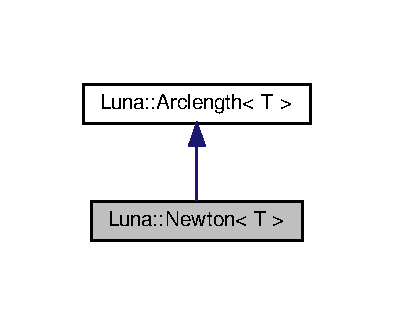
\includegraphics[width=189pt]{classLuna_1_1Newton__inherit__graph}
\end{center}
\end{figure}


Collaboration diagram for Luna\+:\+:Newton$<$ T $>$\+:\nopagebreak
\begin{figure}[H]
\begin{center}
\leavevmode
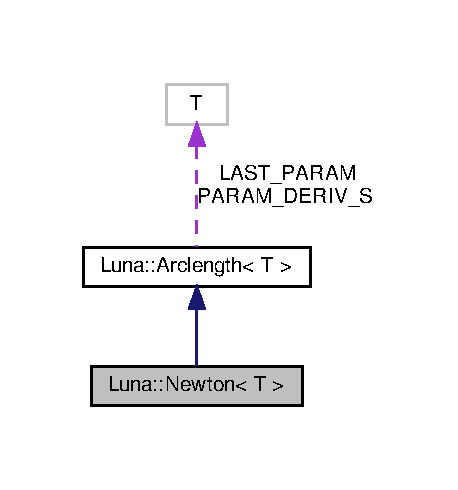
\includegraphics[width=220pt]{classLuna_1_1Newton__coll__graph}
\end{center}
\end{figure}
\subsection*{Public Member Functions}
\begin{DoxyCompactItemize}
\item 
\hyperlink{classLuna_1_1Newton_a062c2b36d5e7d345173c0b2b525b3f9d}{Newton} (\hyperlink{classLuna_1_1Residual}{Residual}$<$ T $>$ $\ast$ptr\+\_\+residual, std\+::size\+\_\+t max\+\_\+iter=20, double tolerance=1.\+0e-\/8, double delta\+\_\+step=1.\+0e-\/8)
\begin{DoxyCompactList}\small\item\em Constructor. \end{DoxyCompactList}\item 
\hyperlink{classLuna_1_1Newton_ad714e7ff295362a3e89bf3cff26dc2da}{$\sim$\+Newton} ()
\begin{DoxyCompactList}\small\item\em Destructor. \end{DoxyCompactList}\item 
void \hyperlink{classLuna_1_1Newton_a3de816dba7a950702b6f93fc710d4f03}{iterate} (\hyperlink{classLuna_1_1Vector}{Vector}$<$ T $>$ \&x\+\_\+0)
\begin{DoxyCompactList}\small\item\em \hyperlink{classLuna_1_1Newton}{Newton} iterate using intial guess x\+\_\+0 (stores the solution in x\+\_\+0) \end{DoxyCompactList}\item 
void \hyperlink{classLuna_1_1Newton_a1d5ebdbfd8910c40ed58244f6348b13e}{solve} (\hyperlink{classLuna_1_1Vector}{Vector}$<$ T $>$ \&x\+\_\+0)
\begin{DoxyCompactList}\small\item\em Solve the system using \hyperlink{classLuna_1_1Newton}{Newton} iteration (points to iterate) \end{DoxyCompactList}\item 
void \hyperlink{classLuna_1_1Newton_ac300f6b5744bf66fd2f385c678d24dcf}{arclength\+\_\+solve} (\hyperlink{classLuna_1_1Vector}{Vector}$<$ T $>$ \&x)
\begin{DoxyCompactList}\small\item\em Arc-\/length solve the system (init\+\_\+arc must be called first) \end{DoxyCompactList}\end{DoxyCompactItemize}
\subsection*{Protected Attributes}
\begin{DoxyCompactItemize}
\item 
\hyperlink{classLuna_1_1Residual}{Residual}$<$ T $>$ $\ast$ \hyperlink{classLuna_1_1Newton_a5cb2983ea8e24c4832a3fb0bdde84b8f}{ptr\+\_\+\+R\+E\+S\+I\+D\+U\+AL}
\item 
std\+::size\+\_\+t \hyperlink{classLuna_1_1Newton_ac8245444273c58c656a78ab0544833ce}{M\+A\+X\+\_\+\+I\+T\+ER}
\item 
double \hyperlink{classLuna_1_1Newton_a13234002150648ac70297ef68a41c9c7}{T\+OL}
\item 
double \hyperlink{classLuna_1_1Newton_ad4862420392d9eb80d135b9c28dd47cb}{D\+E\+L\+TA}
\item 
std\+::size\+\_\+t \hyperlink{classLuna_1_1Newton_a7d549b60ff6d4285d8cbbf6f958c7d88}{O\+R\+D\+ER}
\end{DoxyCompactItemize}
\subsection*{Additional Inherited Members}


\subsection{Detailed Description}
\subsubsection*{template$<$class T$>$\newline
class Luna\+::\+Newton$<$ T $>$}

A templated \hyperlink{classLuna_1_1Newton}{Newton} iteration class. 

Definition at line 24 of file Newton.\+h.



\subsection{Constructor \& Destructor Documentation}
\mbox{\Hypertarget{classLuna_1_1Newton_a062c2b36d5e7d345173c0b2b525b3f9d}\label{classLuna_1_1Newton_a062c2b36d5e7d345173c0b2b525b3f9d}} 
\index{Luna\+::\+Newton@{Luna\+::\+Newton}!Newton@{Newton}}
\index{Newton@{Newton}!Luna\+::\+Newton@{Luna\+::\+Newton}}
\subsubsection{\texorpdfstring{Newton()}{Newton()}}
{\footnotesize\ttfamily template$<$class T$>$ \\
\hyperlink{classLuna_1_1Newton}{Luna\+::\+Newton}$<$ T $>$\+::\hyperlink{classLuna_1_1Newton}{Newton} (\begin{DoxyParamCaption}\item[{\hyperlink{classLuna_1_1Residual}{Residual}$<$ T $>$ $\ast$}]{ptr\+\_\+residual,  }\item[{std\+::size\+\_\+t}]{max\+\_\+iter = {\ttfamily 20},  }\item[{double}]{tolerance = {\ttfamily 1.0e-\/8},  }\item[{double}]{delta\+\_\+step = {\ttfamily 1.0e-\/8} }\end{DoxyParamCaption})\hspace{0.3cm}{\ttfamily [inline]}}



Constructor. 


\begin{DoxyParams}{Parameters}
{\em ptr\+\_\+residual} & Pointer to the residual object \\
\hline
{\em max\+\_\+iter} & Maximum number of iterations \\
\hline
{\em tolerance} & Convergence tolerance \\
\hline
{\em delta\+\_\+step} & Finite-\/difference derivative step \\
\hline
\end{DoxyParams}


Definition at line 39 of file Newton.\+h.


\begin{DoxyCode}
40                                                                       :
41       \hyperlink{classLuna_1_1Newton_a5cb2983ea8e24c4832a3fb0bdde84b8f}{ptr\_RESIDUAL}( ptr\_residual ),
42       \hyperlink{classLuna_1_1Newton_ac8245444273c58c656a78ab0544833ce}{MAX\_ITER}( max\_iter ),
43       \hyperlink{classLuna_1_1Newton_a13234002150648ac70297ef68a41c9c7}{TOL}( tolerance )
44       \{
45         \hyperlink{classLuna_1_1Newton_a5cb2983ea8e24c4832a3fb0bdde84b8f}{ptr\_RESIDUAL} -> delta() = delta\_step;
46         \hyperlink{classLuna_1_1Newton_ad4862420392d9eb80d135b9c28dd47cb}{DELTA} = delta\_step;
47         \hyperlink{classLuna_1_1Newton_a7d549b60ff6d4285d8cbbf6f958c7d88}{ORDER} = \hyperlink{classLuna_1_1Newton_a5cb2983ea8e24c4832a3fb0bdde84b8f}{ptr\_RESIDUAL} -> get\_order();
48       \}
\end{DoxyCode}
\mbox{\Hypertarget{classLuna_1_1Newton_ad714e7ff295362a3e89bf3cff26dc2da}\label{classLuna_1_1Newton_ad714e7ff295362a3e89bf3cff26dc2da}} 
\index{Luna\+::\+Newton@{Luna\+::\+Newton}!````~Newton@{$\sim$\+Newton}}
\index{````~Newton@{$\sim$\+Newton}!Luna\+::\+Newton@{Luna\+::\+Newton}}
\subsubsection{\texorpdfstring{$\sim$\+Newton()}{~Newton()}}
{\footnotesize\ttfamily template$<$class T$>$ \\
\hyperlink{classLuna_1_1Newton}{Luna\+::\+Newton}$<$ T $>$\+::$\sim$\hyperlink{classLuna_1_1Newton}{Newton} (\begin{DoxyParamCaption}{ }\end{DoxyParamCaption})\hspace{0.3cm}{\ttfamily [inline]}}



Destructor. 



Definition at line 51 of file Newton.\+h.



References Luna\+::\+Newton$<$ T $>$\+::iterate().


\begin{DoxyCode}
51 \{\}
\end{DoxyCode}


\subsection{Member Function Documentation}
\mbox{\Hypertarget{classLuna_1_1Newton_ac300f6b5744bf66fd2f385c678d24dcf}\label{classLuna_1_1Newton_ac300f6b5744bf66fd2f385c678d24dcf}} 
\index{Luna\+::\+Newton@{Luna\+::\+Newton}!arclength\+\_\+solve@{arclength\+\_\+solve}}
\index{arclength\+\_\+solve@{arclength\+\_\+solve}!Luna\+::\+Newton@{Luna\+::\+Newton}}
\subsubsection{\texorpdfstring{arclength\+\_\+solve()}{arclength\_solve()}}
{\footnotesize\ttfamily template$<$typename T $>$ \\
void \hyperlink{classLuna_1_1Newton}{Luna\+::\+Newton}$<$ T $>$\+::arclength\+\_\+solve (\begin{DoxyParamCaption}\item[{\hyperlink{classLuna_1_1Vector}{Vector}$<$ T $>$ \&}]{x }\end{DoxyParamCaption})\hspace{0.3cm}{\ttfamily [inline]}}



Arc-\/length solve the system (init\+\_\+arc must be called first) 


\begin{DoxyParams}{Parameters}
{\em x} & The current state \hyperlink{classLuna_1_1Vector}{Vector} \\
\hline
\end{DoxyParams}


Definition at line 107 of file Newton.\+h.



References Luna\+::\+Arclength$<$ T $>$\+::arclength\+\_\+residual(), Luna\+::\+Arclength$<$ T $>$\+::\+A\+R\+C\+S\+T\+E\+P\+\_\+\+M\+U\+L\+T\+I\+P\+L\+I\+ER, Luna\+::\+Newton$<$ T $>$\+::\+D\+E\+L\+TA, Luna\+::\+Vector$<$ T $>$\+::dot(), Luna\+::\+Arclength$<$ T $>$\+::\+DS, Luna\+::\+Arclength$<$ T $>$\+::\+I\+N\+I\+T\+I\+A\+L\+I\+S\+ED, Heat\+\_\+plot\+::J, Luna\+::\+Arclength$<$ T $>$\+::\+Jac\+\_\+arclength\+\_\+residual(), Luna\+::\+Arclength$<$ T $>$\+::\+L\+A\+S\+T\+\_\+\+P\+A\+R\+AM, Luna\+::\+Arclength$<$ T $>$\+::\+L\+A\+S\+T\+\_\+X, Luna\+::\+Arclength$<$ T $>$\+::\+M\+A\+X\+\_\+\+DS, Luna\+::\+Newton$<$ T $>$\+::\+M\+A\+X\+\_\+\+I\+T\+ER, Luna\+::\+Vector$<$ T $>$\+::norm\+\_\+inf(), Luna\+::\+Newton$<$ T $>$\+::\+O\+R\+D\+ER, Luna\+::\+Arclength$<$ T $>$\+::\+P\+A\+R\+A\+M\+\_\+\+D\+E\+R\+I\+V\+\_\+S, Luna\+::\+Arclength$<$ T $>$\+::ptr\+\_\+\+P\+A\+R\+AM, Luna\+::\+Newton$<$ T $>$\+::ptr\+\_\+\+R\+E\+S\+I\+D\+U\+AL, Luna\+::\+Matrix$<$ T $>$\+::solve(), Luna\+::\+Newton$<$ T $>$\+::\+T\+OL, Luna\+::\+Arclength$<$ T $>$\+::update(), Luna\+::\+Arclength$<$ T $>$\+::\+X\+\_\+\+D\+E\+R\+I\+V\+\_\+S, and y.



Referenced by main(), and Luna\+::\+Newton$<$ T $>$\+::solve().


\begin{DoxyCode}
108     \{
109         \textcolor{keywordflow}{if} ( !this->\hyperlink{classLuna_1_1Arclength_a9bf5e636e7a0772f3ba5476ec2c83f6a}{INITIALISED} ) \textcolor{comment}{// Error if init\_arc has not been called}
110         \{
111             \textcolor{keywordflow}{throw} Error( \textcolor{stringliteral}{"Newton arclength\_solve error: not initialised."} );
112         \}
113         Vector<T> backup\_state( \hyperlink{namespaceHeat__plot_aa88370c16b85b784ccbde3ed88bc1991}{x} );
114         T backup\_parameter( *(this->\hyperlink{classLuna_1_1Arclength_a984cead721a38abf1ab2a489052461e0}{ptr\_PARAM}) );
115         \textcolor{keywordtype}{bool} step\_succeeded( \textcolor{keyword}{false} );
116         std::size\_t itn( 0 );
117         \textcolor{comment}{// Guess the next solution}
118         *( this->\hyperlink{classLuna_1_1Arclength_a984cead721a38abf1ab2a489052461e0}{ptr\_PARAM} ) = this->\hyperlink{classLuna_1_1Arclength_a98e8241f24a16ea9f12e514d8d8f841b}{LAST\_PARAM} + this->
      \hyperlink{classLuna_1_1Arclength_a5a02856595774b4a96e4d8add5d9baa4}{PARAM\_DERIV\_S} * this->\hyperlink{classLuna_1_1Arclength_a6797d7b76d3e27c00b9c4c6ab9970405}{DS};
119         \hyperlink{namespaceHeat__plot_aa88370c16b85b784ccbde3ed88bc1991}{x} = this->\hyperlink{classLuna_1_1Arclength_a6d6ba83245b4dd616d265609a93035a2}{LAST\_X} + this->\hyperlink{classLuna_1_1Arclength_a0108e51178f63927883af0b0022c29ad}{X\_DERIV\_S} * this->\hyperlink{classLuna_1_1Arclength_a6797d7b76d3e27c00b9c4c6ab9970405}{DS};
120 
121         Matrix<T> \hyperlink{namespaceHeat__plot_a3cafcec38d886f33b35756791964bb58}{J}( \hyperlink{classLuna_1_1Newton_a7d549b60ff6d4285d8cbbf6f958c7d88}{ORDER}, \hyperlink{classLuna_1_1Newton_a7d549b60ff6d4285d8cbbf6f958c7d88}{ORDER}, 0.0 );
122         Vector<T> R1( \hyperlink{classLuna_1_1Newton_a7d549b60ff6d4285d8cbbf6f958c7d88}{ORDER}, 0.0 );
123         Vector<T> R2( \hyperlink{classLuna_1_1Newton_a7d549b60ff6d4285d8cbbf6f958c7d88}{ORDER}, 0.0 );
124         Vector<T> dR\_dp( \hyperlink{classLuna_1_1Newton_a7d549b60ff6d4285d8cbbf6f958c7d88}{ORDER}, 0.0 );
125         Vector<T> \hyperlink{ODE__BVP__test_8cpp_adf764cbdea00d65edcd07bb9953ad2b7ae1f9fdb8b786c63efc4ce44eeacd17f2}{y}( \hyperlink{classLuna_1_1Newton_a7d549b60ff6d4285d8cbbf6f958c7d88}{ORDER}, 0.0 );
126         Vector<T> z( \hyperlink{classLuna_1_1Newton_a7d549b60ff6d4285d8cbbf6f958c7d88}{ORDER}, 0.0 );
127         Vector<T> JacE;
128 
129         \textcolor{keywordflow}{do}
130         \{
131             this->\hyperlink{classLuna_1_1Newton_a5cb2983ea8e24c4832a3fb0bdde84b8f}{ptr\_RESIDUAL} -> \hyperlink{classLuna_1_1Arclength_a8941ac2150d8a53aaefbf5825553c86b}{update}( \hyperlink{namespaceHeat__plot_aa88370c16b85b784ccbde3ed88bc1991}{x} );              \textcolor{comment}{// Update the residual}
132             \hyperlink{namespaceHeat__plot_a3cafcec38d886f33b35756791964bb58}{J} = this->\hyperlink{classLuna_1_1Newton_a5cb2983ea8e24c4832a3fb0bdde84b8f}{ptr\_RESIDUAL} -> jacobian();           \textcolor{comment}{// Get the Jacobian}
133             R1 = this->\hyperlink{classLuna_1_1Newton_a5cb2983ea8e24c4832a3fb0bdde84b8f}{ptr\_RESIDUAL} -> residual();          \textcolor{comment}{// Get the residual}
134             \textcolor{keywordtype}{double} E1 = \textcolor{keyword}{this} -> \hyperlink{classLuna_1_1Arclength_af47a50bb4ce666b505fe990ab44063db}{arclength\_residual}( \hyperlink{namespaceHeat__plot_aa88370c16b85b784ccbde3ed88bc1991}{x} );    \textcolor{comment}{// Arclength residual}
135             \textcolor{comment}{// Compute derivatives wrt the parameter}
136             *(this->\hyperlink{classLuna_1_1Arclength_a984cead721a38abf1ab2a489052461e0}{ptr\_PARAM}) += this->\hyperlink{classLuna_1_1Newton_ad4862420392d9eb80d135b9c28dd47cb}{DELTA};
137             this->\hyperlink{classLuna_1_1Newton_a5cb2983ea8e24c4832a3fb0bdde84b8f}{ptr\_RESIDUAL} -> residual\_fn( \hyperlink{namespaceHeat__plot_aa88370c16b85b784ccbde3ed88bc1991}{x}, R2 );
138             \textcolor{keywordtype}{double} E2 = \textcolor{keyword}{this} -> \hyperlink{classLuna_1_1Arclength_af47a50bb4ce666b505fe990ab44063db}{arclength\_residual}( \hyperlink{namespaceHeat__plot_aa88370c16b85b784ccbde3ed88bc1991}{x} );
139             *(this->\hyperlink{classLuna_1_1Arclength_a984cead721a38abf1ab2a489052461e0}{ptr\_PARAM}) -= this->\hyperlink{classLuna_1_1Newton_ad4862420392d9eb80d135b9c28dd47cb}{DELTA};
140             dR\_dp = ( R2 - R1 ) / this->\hyperlink{classLuna_1_1Newton_ad4862420392d9eb80d135b9c28dd47cb}{DELTA};
141             T dE\_dp = ( E2 - E1 ) / this->\hyperlink{classLuna_1_1Newton_ad4862420392d9eb80d135b9c28dd47cb}{DELTA};
142             \textcolor{comment}{// Bordering algorithm}
143             \hyperlink{ODE__BVP__test_8cpp_adf764cbdea00d65edcd07bb9953ad2b7ae1f9fdb8b786c63efc4ce44eeacd17f2}{y} = \hyperlink{namespaceHeat__plot_a3cafcec38d886f33b35756791964bb58}{J}.solve( -R1 );
144             z = \hyperlink{namespaceHeat__plot_a3cafcec38d886f33b35756791964bb58}{J}.solve( -dR\_dp );
145             JacE = this->\hyperlink{classLuna_1_1Arclength_a3bffa2fa38c73cd97155289bc902ccc6}{Jac\_arclength\_residual}( \hyperlink{namespaceHeat__plot_aa88370c16b85b784ccbde3ed88bc1991}{x} );
146             T delta\_p = -( E1 + JacE.dot( \hyperlink{ODE__BVP__test_8cpp_adf764cbdea00d65edcd07bb9953ad2b7ae1f9fdb8b786c63efc4ce44eeacd17f2}{y} ) ) / ( dE\_dp + JacE.dot( z ) );
147             Vector<T> delta\_x = \hyperlink{ODE__BVP__test_8cpp_adf764cbdea00d65edcd07bb9953ad2b7ae1f9fdb8b786c63efc4ce44eeacd17f2}{y} + z * delta\_p;
148             \textcolor{keywordtype}{double} max\_correction = std::max( delta\_x.norm\_inf(),
149                                                                                 std::abs( delta\_p ) );
150             \textcolor{keywordflow}{if} ( max\_correction < this->\hyperlink{classLuna_1_1Newton_a13234002150648ac70297ef68a41c9c7}{TOL} )
151             \{
152                 step\_succeeded = \textcolor{keyword}{true};
153                 \textcolor{keywordflow}{break};
154             \}
155             \textcolor{comment}{// Add the corrections to the state variables}
156             \hyperlink{namespaceHeat__plot_aa88370c16b85b784ccbde3ed88bc1991}{x} += delta\_x;
157             *(this->\hyperlink{classLuna_1_1Arclength_a984cead721a38abf1ab2a489052461e0}{ptr\_PARAM}) += delta\_p;
158             ++itn;
159             \textcolor{keywordflow}{if} ( itn > \hyperlink{classLuna_1_1Newton_ac8245444273c58c656a78ab0544833ce}{MAX\_ITER} )
160             \{
161                 step\_succeeded = \textcolor{keyword}{false};
162                 \textcolor{keywordflow}{break};
163             \}
164         \}\textcolor{keywordflow}{while}( \textcolor{keyword}{true} );
165 
166         \textcolor{keywordflow}{if} ( !step\_succeeded )
167         \{
168             \hyperlink{namespaceHeat__plot_aa88370c16b85b784ccbde3ed88bc1991}{x} = backup\_state;                               \textcolor{comment}{// Restore state}
169             *(this->\hyperlink{classLuna_1_1Arclength_a984cead721a38abf1ab2a489052461e0}{ptr\_PARAM}) = backup\_parameter;          \textcolor{comment}{// Restore the parameter}
170             this->\hyperlink{classLuna_1_1Newton_a5cb2983ea8e24c4832a3fb0bdde84b8f}{ptr\_RESIDUAL}->update( \hyperlink{namespaceHeat__plot_aa88370c16b85b784ccbde3ed88bc1991}{x} );                \textcolor{comment}{// Restore the residual}
171             this->DS /= this->\hyperlink{classLuna_1_1Arclength_ae1ff8d41d3e81d9ce335d19de4a269cc}{ARCSTEP\_MULTIPLIER};           \textcolor{comment}{// Reduce our step length}
172 
173         \}
174         \textcolor{keywordflow}{else}
175         \{
176             this->\hyperlink{classLuna_1_1Arclength_a8941ac2150d8a53aaefbf5825553c86b}{update}( \hyperlink{namespaceHeat__plot_aa88370c16b85b784ccbde3ed88bc1991}{x} );
177             \textcolor{keywordflow}{if} ( itn >= 7 )                                 \textcolor{comment}{// Converging to slowly}
178             \{
179                 this->DS /= this->\hyperlink{classLuna_1_1Arclength_ae1ff8d41d3e81d9ce335d19de4a269cc}{ARCSTEP\_MULTIPLIER};
180             \}
181             \textcolor{keywordflow}{if} ( itn <= 2 )                                 \textcolor{comment}{// Converging to quickly}
182             \{
183                 \textcolor{keywordflow}{if} ( std::abs( this->DS * this->\hyperlink{classLuna_1_1Arclength_ae1ff8d41d3e81d9ce335d19de4a269cc}{ARCSTEP\_MULTIPLIER} ) < this->
      \hyperlink{classLuna_1_1Arclength_a8fcd2b977d7ce78342f113d4e69ad8f1}{MAX\_DS} )
184                 \{
185                     this->DS *= this->\hyperlink{classLuna_1_1Arclength_ae1ff8d41d3e81d9ce335d19de4a269cc}{ARCSTEP\_MULTIPLIER};
186                 \}
187             \}
188         \}
189     \}
\end{DoxyCode}
\mbox{\Hypertarget{classLuna_1_1Newton_a3de816dba7a950702b6f93fc710d4f03}\label{classLuna_1_1Newton_a3de816dba7a950702b6f93fc710d4f03}} 
\index{Luna\+::\+Newton@{Luna\+::\+Newton}!iterate@{iterate}}
\index{iterate@{iterate}!Luna\+::\+Newton@{Luna\+::\+Newton}}
\subsubsection{\texorpdfstring{iterate()}{iterate()}}
{\footnotesize\ttfamily template$<$typename T $>$ \\
void \hyperlink{classLuna_1_1Newton}{Luna\+::\+Newton}$<$ T $>$\+::iterate (\begin{DoxyParamCaption}\item[{\hyperlink{classLuna_1_1Vector}{Vector}$<$ T $>$ \&}]{x\+\_\+0 }\end{DoxyParamCaption})\hspace{0.3cm}{\ttfamily [inline]}}



\hyperlink{classLuna_1_1Newton}{Newton} iterate using intial guess x\+\_\+0 (stores the solution in x\+\_\+0) 


\begin{DoxyParams}{Parameters}
{\em x\+\_\+0} & The initial guess \\
\hline
\end{DoxyParams}


Definition at line 73 of file Newton.\+h.



References Heat\+\_\+plot\+::J, Luna\+::\+Newton$<$ T $>$\+::\+M\+A\+X\+\_\+\+I\+T\+ER, Luna\+::\+Vector$<$ T $>$\+::norm\+\_\+inf(), Luna\+::\+Newton$<$ T $>$\+::\+O\+R\+D\+ER, Luna\+::\+Newton$<$ T $>$\+::ptr\+\_\+\+R\+E\+S\+I\+D\+U\+AL, Luna\+::\+Vector$<$ T $>$\+::size(), Luna\+::\+Matrix$<$ T $>$\+::solve(), Luna\+::\+Newton$<$ T $>$\+::\+T\+OL, and Luna\+::\+Arclength$<$ T $>$\+::update().



Referenced by Luna\+::\+Newton$<$ T $>$\+::solve(), and Luna\+::\+Newton$<$ T $>$\+::$\sim$\+Newton().


\begin{DoxyCode}
74     \{
75         \textcolor{comment}{//TODO determinant monitoring etc}
76         \textcolor{keywordflow}{if} ( x\_0.size() != \hyperlink{classLuna_1_1Newton_a7d549b60ff6d4285d8cbbf6f958c7d88}{ORDER} )
77         \{
78             \textcolor{keywordflow}{throw} Error( \textcolor{stringliteral}{"Newton error: size does not agree."} );
79         \}
80         Vector<T> F( \hyperlink{classLuna_1_1Newton_a7d549b60ff6d4285d8cbbf6f958c7d88}{ORDER}, 0.0 );               \textcolor{comment}{// Residual function evaluation}
81         Matrix<T> \hyperlink{namespaceHeat__plot_a3cafcec38d886f33b35756791964bb58}{J}( \hyperlink{classLuna_1_1Newton_a7d549b60ff6d4285d8cbbf6f958c7d88}{ORDER}, \hyperlink{classLuna_1_1Newton_a7d549b60ff6d4285d8cbbf6f958c7d88}{ORDER}, 0.0 );        \textcolor{comment}{// Jacobian matrix}
82         Vector<T> dx( \hyperlink{classLuna_1_1Newton_a7d549b60ff6d4285d8cbbf6f958c7d88}{ORDER}, 0.0 );              \textcolor{comment}{// Increment vector}
83         std::size\_t iter( 0 );
84         \textcolor{keywordtype}{double} max\_residual;
85 
86         \textcolor{keywordflow}{do}
87         \{
88             ++iter;
89             \hyperlink{classLuna_1_1Newton_a5cb2983ea8e24c4832a3fb0bdde84b8f}{ptr\_RESIDUAL} -> \hyperlink{classLuna_1_1Arclength_a8941ac2150d8a53aaefbf5825553c86b}{update}( x\_0 );
90             F = \hyperlink{classLuna_1_1Newton_a5cb2983ea8e24c4832a3fb0bdde84b8f}{ptr\_RESIDUAL} -> residual();
91             max\_residual = F.norm\_inf();
92             \hyperlink{namespaceHeat__plot_a3cafcec38d886f33b35756791964bb58}{J} = \hyperlink{classLuna_1_1Newton_a5cb2983ea8e24c4832a3fb0bdde84b8f}{ptr\_RESIDUAL} -> jacobian();
93 
94             dx = \hyperlink{namespaceHeat__plot_a3cafcec38d886f33b35756791964bb58}{J}.solve( -F );
95             x\_0 += dx;
96         \}\textcolor{keywordflow}{while}( iter < MAX\_ITER && max\_residual > \hyperlink{classLuna_1_1Newton_a13234002150648ac70297ef68a41c9c7}{TOL} );
97 
98         \textcolor{keywordflow}{if} ( iter == \hyperlink{classLuna_1_1Newton_ac8245444273c58c656a78ab0544833ce}{MAX\_ITER} )
99         \{
100             std::string warning;
101             warning = \textcolor{stringliteral}{"NEWTON WARNING! MAXIMUM NUMBER OF ITERATIONS REACHED."};
102             std::cout << warning << std::endl;
103         \}
104     \}
\end{DoxyCode}
\mbox{\Hypertarget{classLuna_1_1Newton_a1d5ebdbfd8910c40ed58244f6348b13e}\label{classLuna_1_1Newton_a1d5ebdbfd8910c40ed58244f6348b13e}} 
\index{Luna\+::\+Newton@{Luna\+::\+Newton}!solve@{solve}}
\index{solve@{solve}!Luna\+::\+Newton@{Luna\+::\+Newton}}
\subsubsection{\texorpdfstring{solve()}{solve()}}
{\footnotesize\ttfamily template$<$class T$>$ \\
void \hyperlink{classLuna_1_1Newton}{Luna\+::\+Newton}$<$ T $>$\+::solve (\begin{DoxyParamCaption}\item[{\hyperlink{classLuna_1_1Vector}{Vector}$<$ T $>$ \&}]{x\+\_\+0 }\end{DoxyParamCaption})\hspace{0.3cm}{\ttfamily [inline]}, {\ttfamily [virtual]}}



Solve the system using \hyperlink{classLuna_1_1Newton}{Newton} iteration (points to iterate) 


\begin{DoxyParams}{Parameters}
{\em x\+\_\+0} & The initial guess \\
\hline
\end{DoxyParams}


Implements \hyperlink{classLuna_1_1Arclength_a0829d51bb49011f5ed56c25b7554d115}{Luna\+::\+Arclength$<$ T $>$}.



Definition at line 61 of file Newton.\+h.



References Luna\+::\+Newton$<$ T $>$\+::arclength\+\_\+solve(), Luna\+::\+Newton$<$ T $>$\+::iterate(), and Heat\+\_\+plot\+::x.



Referenced by main().


\begin{DoxyCode}
62       \{
63         \hyperlink{classLuna_1_1Newton_a3de816dba7a950702b6f93fc710d4f03}{iterate}( x\_0 );
64       \}
\end{DoxyCode}


\subsection{Member Data Documentation}
\mbox{\Hypertarget{classLuna_1_1Newton_ad4862420392d9eb80d135b9c28dd47cb}\label{classLuna_1_1Newton_ad4862420392d9eb80d135b9c28dd47cb}} 
\index{Luna\+::\+Newton@{Luna\+::\+Newton}!D\+E\+L\+TA@{D\+E\+L\+TA}}
\index{D\+E\+L\+TA@{D\+E\+L\+TA}!Luna\+::\+Newton@{Luna\+::\+Newton}}
\subsubsection{\texorpdfstring{D\+E\+L\+TA}{DELTA}}
{\footnotesize\ttfamily template$<$class T$>$ \\
double \hyperlink{classLuna_1_1Newton}{Luna\+::\+Newton}$<$ T $>$\+::D\+E\+L\+TA\hspace{0.3cm}{\ttfamily [protected]}}



Definition at line 30 of file Newton.\+h.



Referenced by Luna\+::\+Newton$<$ T $>$\+::arclength\+\_\+solve().

\mbox{\Hypertarget{classLuna_1_1Newton_ac8245444273c58c656a78ab0544833ce}\label{classLuna_1_1Newton_ac8245444273c58c656a78ab0544833ce}} 
\index{Luna\+::\+Newton@{Luna\+::\+Newton}!M\+A\+X\+\_\+\+I\+T\+ER@{M\+A\+X\+\_\+\+I\+T\+ER}}
\index{M\+A\+X\+\_\+\+I\+T\+ER@{M\+A\+X\+\_\+\+I\+T\+ER}!Luna\+::\+Newton@{Luna\+::\+Newton}}
\subsubsection{\texorpdfstring{M\+A\+X\+\_\+\+I\+T\+ER}{MAX\_ITER}}
{\footnotesize\ttfamily template$<$class T$>$ \\
std\+::size\+\_\+t \hyperlink{classLuna_1_1Newton}{Luna\+::\+Newton}$<$ T $>$\+::M\+A\+X\+\_\+\+I\+T\+ER\hspace{0.3cm}{\ttfamily [protected]}}



Definition at line 28 of file Newton.\+h.



Referenced by Luna\+::\+Newton$<$ T $>$\+::arclength\+\_\+solve(), and Luna\+::\+Newton$<$ T $>$\+::iterate().

\mbox{\Hypertarget{classLuna_1_1Newton_a7d549b60ff6d4285d8cbbf6f958c7d88}\label{classLuna_1_1Newton_a7d549b60ff6d4285d8cbbf6f958c7d88}} 
\index{Luna\+::\+Newton@{Luna\+::\+Newton}!O\+R\+D\+ER@{O\+R\+D\+ER}}
\index{O\+R\+D\+ER@{O\+R\+D\+ER}!Luna\+::\+Newton@{Luna\+::\+Newton}}
\subsubsection{\texorpdfstring{O\+R\+D\+ER}{ORDER}}
{\footnotesize\ttfamily template$<$class T$>$ \\
std\+::size\+\_\+t \hyperlink{classLuna_1_1Newton}{Luna\+::\+Newton}$<$ T $>$\+::O\+R\+D\+ER\hspace{0.3cm}{\ttfamily [protected]}}



Definition at line 31 of file Newton.\+h.



Referenced by Luna\+::\+Newton$<$ T $>$\+::arclength\+\_\+solve(), and Luna\+::\+Newton$<$ T $>$\+::iterate().

\mbox{\Hypertarget{classLuna_1_1Newton_a5cb2983ea8e24c4832a3fb0bdde84b8f}\label{classLuna_1_1Newton_a5cb2983ea8e24c4832a3fb0bdde84b8f}} 
\index{Luna\+::\+Newton@{Luna\+::\+Newton}!ptr\+\_\+\+R\+E\+S\+I\+D\+U\+AL@{ptr\+\_\+\+R\+E\+S\+I\+D\+U\+AL}}
\index{ptr\+\_\+\+R\+E\+S\+I\+D\+U\+AL@{ptr\+\_\+\+R\+E\+S\+I\+D\+U\+AL}!Luna\+::\+Newton@{Luna\+::\+Newton}}
\subsubsection{\texorpdfstring{ptr\+\_\+\+R\+E\+S\+I\+D\+U\+AL}{ptr\_RESIDUAL}}
{\footnotesize\ttfamily template$<$class T$>$ \\
\hyperlink{classLuna_1_1Residual}{Residual}$<$T$>$$\ast$ \hyperlink{classLuna_1_1Newton}{Luna\+::\+Newton}$<$ T $>$\+::ptr\+\_\+\+R\+E\+S\+I\+D\+U\+AL\hspace{0.3cm}{\ttfamily [protected]}}



Definition at line 27 of file Newton.\+h.



Referenced by Luna\+::\+Newton$<$ T $>$\+::arclength\+\_\+solve(), and Luna\+::\+Newton$<$ T $>$\+::iterate().

\mbox{\Hypertarget{classLuna_1_1Newton_a13234002150648ac70297ef68a41c9c7}\label{classLuna_1_1Newton_a13234002150648ac70297ef68a41c9c7}} 
\index{Luna\+::\+Newton@{Luna\+::\+Newton}!T\+OL@{T\+OL}}
\index{T\+OL@{T\+OL}!Luna\+::\+Newton@{Luna\+::\+Newton}}
\subsubsection{\texorpdfstring{T\+OL}{TOL}}
{\footnotesize\ttfamily template$<$class T$>$ \\
double \hyperlink{classLuna_1_1Newton}{Luna\+::\+Newton}$<$ T $>$\+::T\+OL\hspace{0.3cm}{\ttfamily [protected]}}



Definition at line 29 of file Newton.\+h.



Referenced by Luna\+::\+Newton$<$ T $>$\+::arclength\+\_\+solve(), and Luna\+::\+Newton$<$ T $>$\+::iterate().



The documentation for this class was generated from the following file\+:\begin{DoxyCompactItemize}
\item 
include/\+Luna/\hyperlink{Newton_8h}{Newton.\+h}\end{DoxyCompactItemize}

\hypertarget{classLuna_1_1nonlinear__equation}{}\section{Luna\+:\+:nonlinear\+\_\+equation Class Reference}
\label{classLuna_1_1nonlinear__equation}\index{Luna\+::nonlinear\+\_\+equation@{Luna\+::nonlinear\+\_\+equation}}


Inheritance diagram for Luna\+:\+:nonlinear\+\_\+equation\+:\nopagebreak
\begin{figure}[H]
\begin{center}
\leavevmode
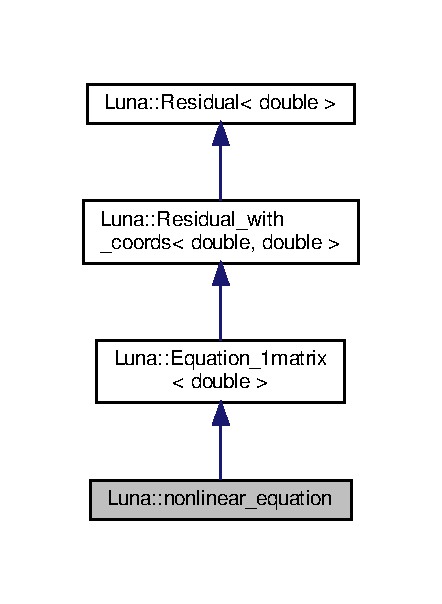
\includegraphics[width=212pt]{classLuna_1_1nonlinear__equation__inherit__graph}
\end{center}
\end{figure}


Collaboration diagram for Luna\+:\+:nonlinear\+\_\+equation\+:\nopagebreak
\begin{figure}[H]
\begin{center}
\leavevmode
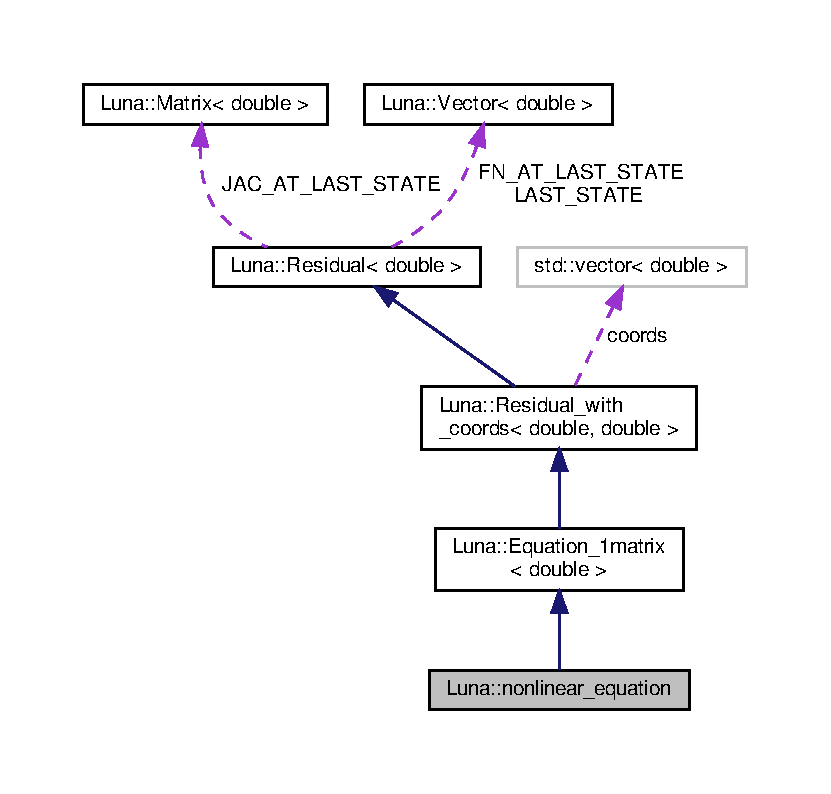
\includegraphics[width=350pt]{classLuna_1_1nonlinear__equation__coll__graph}
\end{center}
\end{figure}
\subsection*{Public Member Functions}
\begin{DoxyCompactItemize}
\item 
\hyperlink{classLuna_1_1nonlinear__equation_ad9742a2d1179a22a9bf369f1ed1ce8ff}{nonlinear\+\_\+equation} ()
\item 
void \hyperlink{classLuna_1_1nonlinear__equation_a5acffbdc83b8b487241cd92b0191be85}{residual\+\_\+fn} (const \hyperlink{classLuna_1_1Vector}{Vector}$<$ double $>$ \&u, \hyperlink{classLuna_1_1Vector}{Vector}$<$ double $>$ \&F) const
\begin{DoxyCompactList}\small\item\em The residual function to be defined later. \end{DoxyCompactList}\item 
void \hyperlink{classLuna_1_1nonlinear__equation_a467d48cbfdb69fddc877e00dc24a397a}{matrix0} (const \hyperlink{classLuna_1_1Vector}{Vector}$<$ double $>$ \&u, \hyperlink{classLuna_1_1Matrix}{Matrix}$<$ double $>$ \&m) const
\begin{DoxyCompactList}\small\item\em Define the matrix in terms of the current state vector. \end{DoxyCompactList}\end{DoxyCompactItemize}
\subsection*{Additional Inherited Members}


\subsection{Detailed Description}


Definition at line 20 of file Nonlinear\+\_\+\+O\+D\+E\+\_\+\+B\+V\+P.\+cpp.



\subsection{Constructor \& Destructor Documentation}
\mbox{\Hypertarget{classLuna_1_1nonlinear__equation_ad9742a2d1179a22a9bf369f1ed1ce8ff}\label{classLuna_1_1nonlinear__equation_ad9742a2d1179a22a9bf369f1ed1ce8ff}} 
\index{Luna\+::nonlinear\+\_\+equation@{Luna\+::nonlinear\+\_\+equation}!nonlinear\+\_\+equation@{nonlinear\+\_\+equation}}
\index{nonlinear\+\_\+equation@{nonlinear\+\_\+equation}!Luna\+::nonlinear\+\_\+equation@{Luna\+::nonlinear\+\_\+equation}}
\subsubsection{\texorpdfstring{nonlinear\+\_\+equation()}{nonlinear\_equation()}}
{\footnotesize\ttfamily Luna\+::nonlinear\+\_\+equation\+::nonlinear\+\_\+equation (\begin{DoxyParamCaption}{ }\end{DoxyParamCaption})\hspace{0.3cm}{\ttfamily [inline]}}



Definition at line 25 of file Nonlinear\+\_\+\+O\+D\+E\+\_\+\+B\+V\+P.\+cpp.


\begin{DoxyCode}
25 : \hyperlink{classLuna_1_1Equation__1matrix}{Equation\_1matrix<double>} ( 2 ) \{\}
\end{DoxyCode}


\subsection{Member Function Documentation}
\mbox{\Hypertarget{classLuna_1_1nonlinear__equation_a467d48cbfdb69fddc877e00dc24a397a}\label{classLuna_1_1nonlinear__equation_a467d48cbfdb69fddc877e00dc24a397a}} 
\index{Luna\+::nonlinear\+\_\+equation@{Luna\+::nonlinear\+\_\+equation}!matrix0@{matrix0}}
\index{matrix0@{matrix0}!Luna\+::nonlinear\+\_\+equation@{Luna\+::nonlinear\+\_\+equation}}
\subsubsection{\texorpdfstring{matrix0()}{matrix0()}}
{\footnotesize\ttfamily void Luna\+::nonlinear\+\_\+equation\+::matrix0 (\begin{DoxyParamCaption}\item[{const \hyperlink{classLuna_1_1Vector}{Vector}$<$ double $>$ \&}]{x,  }\item[{\hyperlink{classLuna_1_1Matrix}{Matrix}$<$ double $>$ \&}]{m }\end{DoxyParamCaption}) const\hspace{0.3cm}{\ttfamily [inline]}, {\ttfamily [virtual]}}



Define the matrix in terms of the current state vector. 


\begin{DoxyParams}{Parameters}
{\em x} & The current state vector. \\
\hline
{\em m} & The matrix. \\
\hline
\end{DoxyParams}


Reimplemented from \hyperlink{classLuna_1_1Equation__1matrix_a2501535a6e92abc491bc491b3f64dc06}{Luna\+::\+Equation\+\_\+1matrix$<$ double $>$}.



Definition at line 35 of file Nonlinear\+\_\+\+O\+D\+E\+\_\+\+B\+V\+P.\+cpp.



References f.


\begin{DoxyCode}
36       \{
37         m( 0, 0 ) = 1.0;
38         m( 1, 1 ) = \hyperlink{namespaceHeat__plot_ae622b86afa46daa3e9b887624ab1bf26}{u}[ \hyperlink{Nonlinear__ODE__BVP_8cpp_a06fc87d81c62e9abb8790b6e5713c55ba7ce756344023b99e5ab27b804feb765c}{f} ] - 1.0;
39       \}
\end{DoxyCode}
\mbox{\Hypertarget{classLuna_1_1nonlinear__equation_a5acffbdc83b8b487241cd92b0191be85}\label{classLuna_1_1nonlinear__equation_a5acffbdc83b8b487241cd92b0191be85}} 
\index{Luna\+::nonlinear\+\_\+equation@{Luna\+::nonlinear\+\_\+equation}!residual\+\_\+fn@{residual\+\_\+fn}}
\index{residual\+\_\+fn@{residual\+\_\+fn}!Luna\+::nonlinear\+\_\+equation@{Luna\+::nonlinear\+\_\+equation}}
\subsubsection{\texorpdfstring{residual\+\_\+fn()}{residual\_fn()}}
{\footnotesize\ttfamily void Luna\+::nonlinear\+\_\+equation\+::residual\+\_\+fn (\begin{DoxyParamCaption}\item[{const \hyperlink{classLuna_1_1Vector}{Vector}$<$ double $>$ \&}]{state,  }\item[{\hyperlink{classLuna_1_1Vector}{Vector}$<$ double $>$ \&}]{f }\end{DoxyParamCaption}) const\hspace{0.3cm}{\ttfamily [inline]}, {\ttfamily [virtual]}}



The residual function to be defined later. 


\begin{DoxyParams}{Parameters}
{\em state} & The current state \hyperlink{classLuna_1_1Vector}{Vector} \\
\hline
{\em f} & The function \hyperlink{classLuna_1_1Vector}{Vector} to be updated \\
\hline
\end{DoxyParams}


Reimplemented from \hyperlink{classLuna_1_1Residual_ae1b1ebe3314c788b176bcac7b328de5c}{Luna\+::\+Residual$<$ double $>$}.



Definition at line 28 of file Nonlinear\+\_\+\+O\+D\+E\+\_\+\+B\+V\+P.\+cpp.



References Luna\+::\+Residual\+\_\+with\+\_\+coords$<$ double, double $>$\+::coord(), f, fd, and Heat\+\_\+plot\+::x.


\begin{DoxyCode}
29             \{
30         \textcolor{keywordtype}{double} \hyperlink{namespaceHeat__plot_aa88370c16b85b784ccbde3ed88bc1991}{x}( \hyperlink{classLuna_1_1Residual__with__coords_a3fa4c950a944743c0380e4c151728372}{coord}( 0 ) );
31                 F[ \hyperlink{Nonlinear__ODE__BVP_8cpp_a06fc87d81c62e9abb8790b6e5713c55ba7ce756344023b99e5ab27b804feb765c}{f} ]   = \hyperlink{namespaceHeat__plot_ae622b86afa46daa3e9b887624ab1bf26}{u}[ \hyperlink{Nonlinear__ODE__BVP_8cpp_a06fc87d81c62e9abb8790b6e5713c55ba1e4d60e5b05464d07a30096747025a42}{fd} ];
32                 F[ \hyperlink{Nonlinear__ODE__BVP_8cpp_a06fc87d81c62e9abb8790b6e5713c55ba1e4d60e5b05464d07a30096747025a42}{fd} ]  = 1. + ( 1. - ( 2. / ( \hyperlink{namespaceHeat__plot_aa88370c16b85b784ccbde3ed88bc1991}{x} * \hyperlink{namespaceHeat__plot_aa88370c16b85b784ccbde3ed88bc1991}{x} ) ) ) * \hyperlink{namespaceHeat__plot_ae622b86afa46daa3e9b887624ab1bf26}{u}[ \hyperlink{Nonlinear__ODE__BVP_8cpp_a06fc87d81c62e9abb8790b6e5713c55ba1e4d60e5b05464d07a30096747025a42}{fd} ] * \hyperlink{namespaceHeat__plot_ae622b86afa46daa3e9b887624ab1bf26}{u}[ 
      \hyperlink{Nonlinear__ODE__BVP_8cpp_a06fc87d81c62e9abb8790b6e5713c55ba1e4d60e5b05464d07a30096747025a42}{fd} ];
33             \}
\end{DoxyCode}


The documentation for this class was generated from the following file\+:\begin{DoxyCompactItemize}
\item 
Examples/\hyperlink{Nonlinear__ODE__BVP_8cpp}{Nonlinear\+\_\+\+O\+D\+E\+\_\+\+B\+V\+P.\+cpp}\end{DoxyCompactItemize}

\hypertarget{classLuna_1_1ODE__BVP}{}\section{Luna\+:\+:O\+D\+E\+\_\+\+B\+VP$<$ T, X $>$ Class Template Reference}
\label{classLuna_1_1ODE__BVP}\index{Luna\+::\+O\+D\+E\+\_\+\+B\+V\+P$<$ T, X $>$@{Luna\+::\+O\+D\+E\+\_\+\+B\+V\+P$<$ T, X $>$}}


A templated object for boundary-\/value problems as systems of first-\/order ordinary differential equations.  




{\ttfamily \#include $<$O\+D\+E\+\_\+\+B\+V\+P.\+h$>$}

\subsection*{Public Member Functions}
\begin{DoxyCompactItemize}
\item 
\hyperlink{classLuna_1_1ODE__BVP_adc692c5395375409ac3df8ec8b9ec32b}{O\+D\+E\+\_\+\+B\+VP} (\hyperlink{classLuna_1_1Equation__1matrix}{Equation\+\_\+1matrix}$<$ T, X $>$ $\ast$ptr\+\_\+equation, const \hyperlink{classLuna_1_1Vector}{Vector}$<$ X $>$ \&nodes, \hyperlink{classLuna_1_1Residual}{Residual}$<$ T $>$ $\ast$ptr\+\_\+left\+\_\+residual, \hyperlink{classLuna_1_1Residual}{Residual}$<$ T $>$ $\ast$ptr\+\_\+right\+\_\+residual)
\begin{DoxyCompactList}\small\item\em Constructor. \end{DoxyCompactList}\item 
virtual \hyperlink{classLuna_1_1ODE__BVP_af4ad8cb4bd83a9e41c02bbcf8d28022e}{$\sim$\+O\+D\+E\+\_\+\+B\+VP} ()
\begin{DoxyCompactList}\small\item\em Destructor. \end{DoxyCompactList}\item 
\hyperlink{classLuna_1_1Mesh1D}{Mesh1D}$<$ T, X $>$ \& \hyperlink{classLuna_1_1ODE__BVP_af869c5d4c32de3e2c6dce128f86379a7}{solution} ()
\begin{DoxyCompactList}\small\item\em Return a pointer to the current solution mesh. \end{DoxyCompactList}\item 
double \& \hyperlink{classLuna_1_1ODE__BVP_a9b3eeb599a5d12ebb6bab1b80ff02844}{tolerance} ()
\begin{DoxyCompactList}\small\item\em Access the tolerance for convergence. \end{DoxyCompactList}\item 
int \& \hyperlink{classLuna_1_1ODE__BVP_ad013352e3aa277825cbac01d6334554b}{max\+\_\+iterations} ()
\begin{DoxyCompactList}\small\item\em Access the maximum number of iterations. \end{DoxyCompactList}\item 
void \hyperlink{classLuna_1_1ODE__BVP_a6bf2f309333522cf1a4d251580ee56d5}{set\+\_\+monitor\+\_\+det} (bool monitor)
\begin{DoxyCompactList}\small\item\em Set whether the determinant will be monitored. \end{DoxyCompactList}\item 
void \hyperlink{classLuna_1_1ODE__BVP_ae035272ad664be6ad5334f1b93a86b15}{solve\+\_\+bvp} ()
\begin{DoxyCompactList}\small\item\em Solve the boundary value problem. \end{DoxyCompactList}\item 
std\+::pair$<$ unsigned, unsigned $>$ \hyperlink{classLuna_1_1ODE__BVP_af132e3f1f22a87bd2505c556cd6e0993}{adapt} (const double \&adapt\+\_\+tol)
\begin{DoxyCompactList}\small\item\em Adapt the computational mesh. \end{DoxyCompactList}\item 
void \hyperlink{classLuna_1_1ODE__BVP_a504f92ae04c8ab1ccd2b1ba96c09b79e}{adapt\+\_\+until} (const double \&adapt\+\_\+tol)
\begin{DoxyCompactList}\small\item\em Solve the system with mesh refinements or unrefinements. \end{DoxyCompactList}\item 
{\footnotesize template$<$$>$ }\\std\+::pair$<$ unsigned, unsigned $>$ \hyperlink{classLuna_1_1ODE__BVP_a8da2eba83d2bb58a5e87f77ce3620056}{adapt} (const double \&adapt\+\_\+tol)
\item 
{\footnotesize template$<$$>$ }\\std\+::pair$<$ unsigned, unsigned $>$ \hyperlink{classLuna_1_1ODE__BVP_a59d055c7eb9058184aa86d5514d615e5}{adapt} (const double \&adapt\+\_\+tol)
\item 
{\footnotesize template$<$$>$ }\\void \hyperlink{classLuna_1_1ODE__BVP_a5158d9bd406cfea3eaa7f98f5fc74d44}{adapt\+\_\+until} (const double \&adapt\+\_\+tol)
\item 
{\footnotesize template$<$$>$ }\\void \hyperlink{classLuna_1_1ODE__BVP_a5127af573d557a9640fdff989e9f7e69}{adapt\+\_\+until} (const double \&adapt\+\_\+tol)
\end{DoxyCompactItemize}


\subsection{Detailed Description}
\subsubsection*{template$<$class T, class X = double$>$\newline
class Luna\+::\+O\+D\+E\+\_\+\+B\+V\+P$<$ T, X $>$}

A templated object for boundary-\/value problems as systems of first-\/order ordinary differential equations. 



Definition at line 51 of file O\+D\+E\+\_\+\+B\+V\+P.\+h.



\subsection{Constructor \& Destructor Documentation}
\mbox{\Hypertarget{classLuna_1_1ODE__BVP_adc692c5395375409ac3df8ec8b9ec32b}\label{classLuna_1_1ODE__BVP_adc692c5395375409ac3df8ec8b9ec32b}} 
\index{Luna\+::\+O\+D\+E\+\_\+\+B\+VP@{Luna\+::\+O\+D\+E\+\_\+\+B\+VP}!O\+D\+E\+\_\+\+B\+VP@{O\+D\+E\+\_\+\+B\+VP}}
\index{O\+D\+E\+\_\+\+B\+VP@{O\+D\+E\+\_\+\+B\+VP}!Luna\+::\+O\+D\+E\+\_\+\+B\+VP@{Luna\+::\+O\+D\+E\+\_\+\+B\+VP}}
\subsubsection{\texorpdfstring{O\+D\+E\+\_\+\+B\+V\+P()}{ODE\_BVP()}}
{\footnotesize\ttfamily template$<$typename T , typename X $>$ \\
\hyperlink{classLuna_1_1ODE__BVP}{Luna\+::\+O\+D\+E\+\_\+\+B\+VP}$<$ T, X $>$\+::\hyperlink{classLuna_1_1ODE__BVP}{O\+D\+E\+\_\+\+B\+VP} (\begin{DoxyParamCaption}\item[{\hyperlink{classLuna_1_1Equation__1matrix}{Equation\+\_\+1matrix}$<$ T, X $>$ $\ast$}]{ptr\+\_\+equation,  }\item[{const \hyperlink{classLuna_1_1Vector}{Vector}$<$ X $>$ \&}]{nodes,  }\item[{\hyperlink{classLuna_1_1Residual}{Residual}$<$ T $>$ $\ast$}]{ptr\+\_\+left\+\_\+residual,  }\item[{\hyperlink{classLuna_1_1Residual}{Residual}$<$ T $>$ $\ast$}]{ptr\+\_\+right\+\_\+residual }\end{DoxyParamCaption})}



Constructor. 



Definition at line 117 of file O\+D\+E\+\_\+\+B\+V\+P.\+h.


\begin{DoxyCode}
119                                              :
120            MAX\_ITER( 20 ), TOL( 1e-8 ), ptr\_EQUATION( ptr\_equation ),
121            ptr\_LEFT\_RESIDUAL( ptr\_left\_residual ),
122            ptr\_RIGHT\_RESIDUAL( ptr\_right\_residual ),
123            LAST\_DET\_SIGN( 0 ), MONITOR\_DET( \textcolor{keyword}{true} )
124   \{
125     SOLUTION = Mesh1D<T, X>( nodes, ptr\_EQUATION -> get\_order() );
126 
127     \textcolor{keywordtype}{unsigned} eqn\_order( ptr\_EQUATION -> get\_order() );
128     \textcolor{keywordtype}{unsigned} left\_vars( ptr\_LEFT\_RESIDUAL -> get\_number\_of\_vars() );
129     \textcolor{keywordtype}{unsigned} right\_vars( ptr\_RIGHT\_RESIDUAL -> get\_number\_of\_vars() );
130     \textcolor{keywordtype}{unsigned} left\_order( ptr\_LEFT\_RESIDUAL -> get\_order() );
131     \textcolor{keywordtype}{unsigned} right\_order( ptr\_RIGHT\_RESIDUAL -> get\_order() );
132 
133     \textcolor{keywordflow}{if} ( ( left\_vars != eqn\_order ) || ( right\_vars != eqn\_order ) ||
134          ( left\_order + right\_order != eqn\_order ) )
135     \{
136      std::cout << \textcolor{stringliteral}{"order "} << eqn\_order << std::endl;
137      std::cout << \textcolor{stringliteral}{"left nvars "} << left\_vars << std::endl;
138      std::cout << \textcolor{stringliteral}{"right nvars "} << right\_vars << std::endl;
139      std::cout << \textcolor{stringliteral}{"left order "} << left\_order << std::endl;
140      std::cout << \textcolor{stringliteral}{"right order "} << right\_order << std::endl;
141      std::string problem;
142      problem  = \textcolor{stringliteral}{"The ODE\_BVP equation and boundary conditions are not well\(\backslash\)n"};
143      problem += \textcolor{stringliteral}{"posed. The number of variables for each boundary condition\(\backslash\)n"};
144      problem += \textcolor{stringliteral}{"has to be the same as the order of the equation. Also the \(\backslash\)n"};
145      problem += \textcolor{stringliteral}{"order of both boundary conditions has to sum to the order\(\backslash\)n"};
146      problem += \textcolor{stringliteral}{"of the equation.\(\backslash\)n"};
147      \textcolor{keywordflow}{throw} Error( problem );
148     \}
149   \}
\end{DoxyCode}
\mbox{\Hypertarget{classLuna_1_1ODE__BVP_af4ad8cb4bd83a9e41c02bbcf8d28022e}\label{classLuna_1_1ODE__BVP_af4ad8cb4bd83a9e41c02bbcf8d28022e}} 
\index{Luna\+::\+O\+D\+E\+\_\+\+B\+VP@{Luna\+::\+O\+D\+E\+\_\+\+B\+VP}!````~O\+D\+E\+\_\+\+B\+VP@{$\sim$\+O\+D\+E\+\_\+\+B\+VP}}
\index{````~O\+D\+E\+\_\+\+B\+VP@{$\sim$\+O\+D\+E\+\_\+\+B\+VP}!Luna\+::\+O\+D\+E\+\_\+\+B\+VP@{Luna\+::\+O\+D\+E\+\_\+\+B\+VP}}
\subsubsection{\texorpdfstring{$\sim$\+O\+D\+E\+\_\+\+B\+V\+P()}{~ODE\_BVP()}}
{\footnotesize\ttfamily template$<$typename T , typename X $>$ \\
\hyperlink{classLuna_1_1ODE__BVP}{Luna\+::\+O\+D\+E\+\_\+\+B\+VP}$<$ T, X $>$\+::$\sim$\hyperlink{classLuna_1_1ODE__BVP}{O\+D\+E\+\_\+\+B\+VP} (\begin{DoxyParamCaption}{ }\end{DoxyParamCaption})\hspace{0.3cm}{\ttfamily [virtual]}}



Destructor. 



Definition at line 152 of file O\+D\+E\+\_\+\+B\+V\+P.\+h.


\begin{DoxyCode}
153     \{\}
\end{DoxyCode}


\subsection{Member Function Documentation}
\mbox{\Hypertarget{classLuna_1_1ODE__BVP_af132e3f1f22a87bd2505c556cd6e0993}\label{classLuna_1_1ODE__BVP_af132e3f1f22a87bd2505c556cd6e0993}} 
\index{Luna\+::\+O\+D\+E\+\_\+\+B\+VP@{Luna\+::\+O\+D\+E\+\_\+\+B\+VP}!adapt@{adapt}}
\index{adapt@{adapt}!Luna\+::\+O\+D\+E\+\_\+\+B\+VP@{Luna\+::\+O\+D\+E\+\_\+\+B\+VP}}
\subsubsection{\texorpdfstring{adapt()}{adapt()}\hspace{0.1cm}{\footnotesize\ttfamily [1/3]}}
{\footnotesize\ttfamily template$<$typename T , typename X $>$ \\
std\+::pair$<$ unsigned, unsigned $>$ \hyperlink{classLuna_1_1ODE__BVP}{Luna\+::\+O\+D\+E\+\_\+\+B\+VP}$<$ T, X $>$\+::adapt (\begin{DoxyParamCaption}\item[{const double \&}]{adapt\+\_\+tol }\end{DoxyParamCaption})}



Adapt the computational mesh. 


\begin{DoxyParams}{Parameters}
{\em adapt\+\_\+tol} & The residual tolerance at a nodal point to determine whether mesh refinements will occur \\
\hline
\end{DoxyParams}
\begin{DoxyReturn}{Returns}
A pair of values indicating the number of refinements and unrefinements. 
\end{DoxyReturn}


Definition at line 261 of file O\+D\+E\+\_\+\+B\+V\+P.\+h.



References Heat\+\_\+plot\+::N, Luna\+::\+Vector$<$ T $>$\+::norm\+\_\+inf(), and Luna\+::\+Vector$<$ T $>$\+::push\+\_\+back().



Referenced by Luna\+::\+O\+D\+E\+\_\+\+B\+V\+P$<$ T, X $>$\+::adapt\+\_\+until().


\begin{DoxyCode}
262   \{
263     \textcolor{keywordtype}{unsigned} order( ptr\_EQUATION -> get\_order() );
264     \textcolor{keywordtype}{unsigned} \hyperlink{namespaceHeat__plot_a7d050092798e28458a263710837bda77}{N}( SOLUTION.nnodes() );
265 
266     Vector<T> F\_node( order, 0.0 );
267     Vector<T> R\_node( order, 0.0 );
268 
269     std::vector<bool> refine( \hyperlink{namespaceHeat__plot_a7d050092798e28458a263710837bda77}{N}, \textcolor{keyword}{false} );
270     std::vector<bool> unrefine( \hyperlink{namespaceHeat__plot_a7d050092798e28458a263710837bda77}{N}, \textcolor{keyword}{false} );
271 
272     Vector<double> Res2( \hyperlink{namespaceHeat__plot_a7d050092798e28458a263710837bda77}{N}, 0.0 );
273 
274     \textcolor{keywordflow}{for} ( std::size\_t node = 1; node <= \hyperlink{namespaceHeat__plot_a7d050092798e28458a263710837bda77}{N} - 2; node += 2 )
275     \{
276       \textcolor{comment}{// set the current solution at this node}
277       \textcolor{keywordflow}{for} ( \textcolor{keywordtype}{unsigned} var = 0; var < order; ++var )
278       \{
279          F\_node[ var ] = SOLUTION( node, var );
280       \}
281       \textcolor{comment}{// set the y-pos in the eqn}
282       ptr\_EQUATION -> coord(0) = SOLUTION.coord( node );
283       \textcolor{comment}{// Update the equation to the nodal position}
284       ptr\_EQUATION -> update( F\_node );
285       \textcolor{comment}{// step size centred at the node}
286       X invh = 1. / ( SOLUTION.coord( node + 1 ) - SOLUTION.coord( node - 1 ) );
287       \textcolor{comment}{// loop over all the variables}
288       Vector<T> temp( order, 0.0 );
289       \textcolor{keywordflow}{for} ( \textcolor{keywordtype}{unsigned} var = 0; var < order; ++var )
290       \{
291         temp[ var ] = ptr\_EQUATION -> residual()[ var ] - (
292                 SOLUTION( node + 1, var ) - SOLUTION( node - 1, var ) ) * invh;
293       \}
294       Res2[ node ] = temp.norm\_inf();
295       \textcolor{keywordflow}{if} ( Res2[ node ] > adapt\_tol )
296       \{
297         refine[ node ] = \textcolor{keyword}{true};
298       \}
299       \textcolor{keywordflow}{else} \textcolor{keywordflow}{if} ( Res2[ node ] < TOL / 10. )
300       \{
301         unrefine[ node ] = \textcolor{keyword}{true};
302       \}
303     \}
304 
305     std::size\_t no\_refined( 0 ), no\_unrefined( 0 );
306     \textcolor{keywordflow}{for} ( std::size\_t i = 0; i < refine.size(); ++i )
307     \{
308       \textcolor{keywordflow}{if} ( refine[ i ] == \textcolor{keyword}{true} )\{ no\_refined++; \}
309       \textcolor{keywordflow}{if} ( unrefine[ i ] == \textcolor{keyword}{true} )\{ no\_unrefined++; \}
310     \}
311 
312     \textcolor{comment}{// make a new refined/unrefined mesh}
313     Vector<X> nodes( SOLUTION.nodes() );
314     Vector<X> newX;
315     newX.push\_back( nodes[ 0 ] );
316     \textcolor{keywordflow}{for} ( std::size\_t i = 1; i < \hyperlink{namespaceHeat__plot_a7d050092798e28458a263710837bda77}{N} - 1; ++i )
317     \{
318       \textcolor{keywordflow}{if} ( refine[ i ] )
319       \{
320         \textcolor{keywordflow}{if} ( !refine[ i - 1 ] )
321         \{
322           \textcolor{comment}{// Have not already refined to the left}
323           \textcolor{comment}{// so refine left AND right with new nodes}
324           X left( nodes[ i - 1 ] );
325           X right( nodes[ i + 1 ] );
326           X here( nodes[ i ] );
327           newX.push\_back( ( left + here ) / 2. );
328           newX.push\_back( here );
329           newX.push\_back( ( right + here ) / 2. );
330         \}
331         \textcolor{keywordflow}{else}
332         \{
333           \textcolor{comment}{// already left refined, so just refine right}
334           X right( nodes[ i + 1 ] );
335           X here( nodes[ i ] );
336           newX.push\_back( here );
337           newX.push\_back( ( right + here ) / 2. );
338         \}
339       \}
340       \textcolor{keywordflow}{else} \textcolor{keywordflow}{if} ( !unrefine[ i ] )
341       \{
342         newX.push\_back( nodes[ i ] );
343       \}
344     \}
345     newX.push\_back( nodes[ N - 1 ] );
346 
347     SOLUTION.remesh( newX );
348 
349     LAST\_DET\_SIGN = 0;
350 
351     std::pair< unsigned, unsigned > feedback;
352     feedback.first = no\_refined;
353     feedback.second = no\_unrefined;
354     \textcolor{keywordflow}{return} feedback;
355   \}
\end{DoxyCode}
\mbox{\Hypertarget{classLuna_1_1ODE__BVP_a8da2eba83d2bb58a5e87f77ce3620056}\label{classLuna_1_1ODE__BVP_a8da2eba83d2bb58a5e87f77ce3620056}} 
\index{Luna\+::\+O\+D\+E\+\_\+\+B\+VP@{Luna\+::\+O\+D\+E\+\_\+\+B\+VP}!adapt@{adapt}}
\index{adapt@{adapt}!Luna\+::\+O\+D\+E\+\_\+\+B\+VP@{Luna\+::\+O\+D\+E\+\_\+\+B\+VP}}
\subsubsection{\texorpdfstring{adapt()}{adapt()}\hspace{0.1cm}{\footnotesize\ttfamily [2/3]}}
{\footnotesize\ttfamily template$<$$>$ \\
std\+::pair$<$ unsigned, unsigned $>$ \hyperlink{classLuna_1_1ODE__BVP}{Luna\+::\+O\+D\+E\+\_\+\+B\+VP}$<$ double, \hyperlink{namespaceLuna_af3257e90072a78a8ffb16a16773aa18e}{cmplx} $>$\+::adapt (\begin{DoxyParamCaption}\item[{const double \&}]{adapt\+\_\+tol }\end{DoxyParamCaption})}



Definition at line 239 of file O\+D\+E\+\_\+\+B\+V\+P.\+h.


\begin{DoxyCode}
241   \{
242     std::string problem;
243     problem = \textcolor{stringliteral}{" The ODE\_BVP.adapt method has been called for a problem in \(\backslash\)n"};
244     problem += \textcolor{stringliteral}{" the complex plane. This doesn't make sense as the path is \(\backslash\)n"};
245     problem += \textcolor{stringliteral}{" not geometrically defined. \(\backslash\)n"};
246     \textcolor{keywordflow}{throw} Error( problem );
247   \}
\end{DoxyCode}
\mbox{\Hypertarget{classLuna_1_1ODE__BVP_a59d055c7eb9058184aa86d5514d615e5}\label{classLuna_1_1ODE__BVP_a59d055c7eb9058184aa86d5514d615e5}} 
\index{Luna\+::\+O\+D\+E\+\_\+\+B\+VP@{Luna\+::\+O\+D\+E\+\_\+\+B\+VP}!adapt@{adapt}}
\index{adapt@{adapt}!Luna\+::\+O\+D\+E\+\_\+\+B\+VP@{Luna\+::\+O\+D\+E\+\_\+\+B\+VP}}
\subsubsection{\texorpdfstring{adapt()}{adapt()}\hspace{0.1cm}{\footnotesize\ttfamily [3/3]}}
{\footnotesize\ttfamily template$<$$>$ \\
std\+::pair$<$ unsigned, unsigned $>$ \hyperlink{classLuna_1_1ODE__BVP}{Luna\+::\+O\+D\+E\+\_\+\+B\+VP}$<$ \hyperlink{namespaceLuna_af3257e90072a78a8ffb16a16773aa18e}{cmplx}, \hyperlink{namespaceLuna_af3257e90072a78a8ffb16a16773aa18e}{cmplx} $>$\+::adapt (\begin{DoxyParamCaption}\item[{const double \&}]{adapt\+\_\+tol }\end{DoxyParamCaption})}



Definition at line 250 of file O\+D\+E\+\_\+\+B\+V\+P.\+h.


\begin{DoxyCode}
252   \{
253     std::string problem;
254     problem = \textcolor{stringliteral}{" The ODE\_BVP.adapt method has been called for a problem in \(\backslash\)n"};
255     problem += \textcolor{stringliteral}{" the complex plane. This doesn't make sense as the path is \(\backslash\)n"};
256     problem += \textcolor{stringliteral}{" not geometrically defined. \(\backslash\)n"};
257     \textcolor{keywordflow}{throw} Error( problem );
258   \}
\end{DoxyCode}
\mbox{\Hypertarget{classLuna_1_1ODE__BVP_a504f92ae04c8ab1ccd2b1ba96c09b79e}\label{classLuna_1_1ODE__BVP_a504f92ae04c8ab1ccd2b1ba96c09b79e}} 
\index{Luna\+::\+O\+D\+E\+\_\+\+B\+VP@{Luna\+::\+O\+D\+E\+\_\+\+B\+VP}!adapt\+\_\+until@{adapt\+\_\+until}}
\index{adapt\+\_\+until@{adapt\+\_\+until}!Luna\+::\+O\+D\+E\+\_\+\+B\+VP@{Luna\+::\+O\+D\+E\+\_\+\+B\+VP}}
\subsubsection{\texorpdfstring{adapt\+\_\+until()}{adapt\_until()}\hspace{0.1cm}{\footnotesize\ttfamily [1/3]}}
{\footnotesize\ttfamily template$<$typename T , typename X $>$ \\
void \hyperlink{classLuna_1_1ODE__BVP}{Luna\+::\+O\+D\+E\+\_\+\+B\+VP}$<$ T, X $>$\+::adapt\+\_\+until (\begin{DoxyParamCaption}\item[{const double \&}]{adapt\+\_\+tol }\end{DoxyParamCaption})}



Solve the system with mesh refinements or unrefinements. 


\begin{DoxyParams}{Parameters}
{\em adapt\+\_\+tol} & The residual tolerance at a nodal point to determine whether mesh refinements will occur \\
\hline
\end{DoxyParams}


Definition at line 378 of file O\+D\+E\+\_\+\+B\+V\+P.\+h.



References Luna\+::\+O\+D\+E\+\_\+\+B\+V\+P$<$ T, X $>$\+::adapt(), Luna\+::\+Vector$<$ T $>$\+::dot(), Luna\+::\+Banded\+Matrix$<$ T $>$\+::fill(), and Luna\+::\+O\+D\+E\+\_\+\+B\+V\+P$<$ T, X $>$\+::solve\+\_\+bvp().


\begin{DoxyCode}
379   \{
380     std::pair<unsigned, unsigned> changes;
381     \textcolor{keywordflow}{do} \{
382       changes = \hyperlink{classLuna_1_1ODE__BVP_af132e3f1f22a87bd2505c556cd6e0993}{adapt}( adapt\_tol );
383       \hyperlink{classLuna_1_1ODE__BVP_ae035272ad664be6ad5334f1b93a86b15}{solve\_bvp}();
384       std::cout << \textcolor{stringliteral}{" * Adapting: "} << changes.first << \textcolor{stringliteral}{" "} << changes.second
385                 << std::endl;
386     \}\textcolor{keywordflow}{while} ( changes.first + changes.second != 0 );
387   \}
\end{DoxyCode}
\mbox{\Hypertarget{classLuna_1_1ODE__BVP_a5158d9bd406cfea3eaa7f98f5fc74d44}\label{classLuna_1_1ODE__BVP_a5158d9bd406cfea3eaa7f98f5fc74d44}} 
\index{Luna\+::\+O\+D\+E\+\_\+\+B\+VP@{Luna\+::\+O\+D\+E\+\_\+\+B\+VP}!adapt\+\_\+until@{adapt\+\_\+until}}
\index{adapt\+\_\+until@{adapt\+\_\+until}!Luna\+::\+O\+D\+E\+\_\+\+B\+VP@{Luna\+::\+O\+D\+E\+\_\+\+B\+VP}}
\subsubsection{\texorpdfstring{adapt\+\_\+until()}{adapt\_until()}\hspace{0.1cm}{\footnotesize\ttfamily [2/3]}}
{\footnotesize\ttfamily template$<$$>$ \\
void \hyperlink{classLuna_1_1ODE__BVP}{Luna\+::\+O\+D\+E\+\_\+\+B\+VP}$<$ double, \hyperlink{namespaceLuna_af3257e90072a78a8ffb16a16773aa18e}{cmplx} $>$\+::adapt\+\_\+until (\begin{DoxyParamCaption}\item[{const double \&}]{adapt\+\_\+tol }\end{DoxyParamCaption})}



Definition at line 358 of file O\+D\+E\+\_\+\+B\+V\+P.\+h.


\begin{DoxyCode}
359   \{
360     std::string problem;
361     problem = \textcolor{stringliteral}{" The ODE\_BVP.adapt\_until method has been called for a problem\(\backslash\)n"};
362     problem += \textcolor{stringliteral}{" in the complex plane. This doesn't make sense as the path\(\backslash\)n"};
363     problem += \textcolor{stringliteral}{" is not geometrically defined. \(\backslash\)n"};
364     \textcolor{keywordflow}{throw} Error( problem );
365   \}
\end{DoxyCode}
\mbox{\Hypertarget{classLuna_1_1ODE__BVP_a5127af573d557a9640fdff989e9f7e69}\label{classLuna_1_1ODE__BVP_a5127af573d557a9640fdff989e9f7e69}} 
\index{Luna\+::\+O\+D\+E\+\_\+\+B\+VP@{Luna\+::\+O\+D\+E\+\_\+\+B\+VP}!adapt\+\_\+until@{adapt\+\_\+until}}
\index{adapt\+\_\+until@{adapt\+\_\+until}!Luna\+::\+O\+D\+E\+\_\+\+B\+VP@{Luna\+::\+O\+D\+E\+\_\+\+B\+VP}}
\subsubsection{\texorpdfstring{adapt\+\_\+until()}{adapt\_until()}\hspace{0.1cm}{\footnotesize\ttfamily [3/3]}}
{\footnotesize\ttfamily template$<$$>$ \\
void \hyperlink{classLuna_1_1ODE__BVP}{Luna\+::\+O\+D\+E\+\_\+\+B\+VP}$<$ \hyperlink{namespaceLuna_af3257e90072a78a8ffb16a16773aa18e}{cmplx}, \hyperlink{namespaceLuna_af3257e90072a78a8ffb16a16773aa18e}{cmplx} $>$\+::adapt\+\_\+until (\begin{DoxyParamCaption}\item[{const double \&}]{adapt\+\_\+tol }\end{DoxyParamCaption})}



Definition at line 368 of file O\+D\+E\+\_\+\+B\+V\+P.\+h.


\begin{DoxyCode}
369   \{
370     std::string problem;
371     problem = \textcolor{stringliteral}{" The ODE\_BVP.adapt\_until method has been called for a problem\(\backslash\)n"};
372     problem += \textcolor{stringliteral}{" in the complex plane. This doesn't make sense as the path\(\backslash\)n"};
373     problem += \textcolor{stringliteral}{" is not geometrically defined. \(\backslash\)n"};
374     \textcolor{keywordflow}{throw} Error( problem );
375   \}
\end{DoxyCode}
\mbox{\Hypertarget{classLuna_1_1ODE__BVP_ad013352e3aa277825cbac01d6334554b}\label{classLuna_1_1ODE__BVP_ad013352e3aa277825cbac01d6334554b}} 
\index{Luna\+::\+O\+D\+E\+\_\+\+B\+VP@{Luna\+::\+O\+D\+E\+\_\+\+B\+VP}!max\+\_\+iterations@{max\+\_\+iterations}}
\index{max\+\_\+iterations@{max\+\_\+iterations}!Luna\+::\+O\+D\+E\+\_\+\+B\+VP@{Luna\+::\+O\+D\+E\+\_\+\+B\+VP}}
\subsubsection{\texorpdfstring{max\+\_\+iterations()}{max\_iterations()}}
{\footnotesize\ttfamily template$<$typename T , typename X $>$ \\
int \& \hyperlink{classLuna_1_1ODE__BVP}{Luna\+::\+O\+D\+E\+\_\+\+B\+VP}$<$ T, X $>$\+::max\+\_\+iterations (\begin{DoxyParamCaption}{ }\end{DoxyParamCaption})}



Access the maximum number of iterations. 

\begin{DoxyReturn}{Returns}
a pointer to the maximum number of iterations 
\end{DoxyReturn}


Definition at line 170 of file O\+D\+E\+\_\+\+B\+V\+P.\+h.



Referenced by main().


\begin{DoxyCode}
171   \{
172     \textcolor{keywordflow}{return} MAX\_ITER;
173   \}
\end{DoxyCode}
\mbox{\Hypertarget{classLuna_1_1ODE__BVP_a6bf2f309333522cf1a4d251580ee56d5}\label{classLuna_1_1ODE__BVP_a6bf2f309333522cf1a4d251580ee56d5}} 
\index{Luna\+::\+O\+D\+E\+\_\+\+B\+VP@{Luna\+::\+O\+D\+E\+\_\+\+B\+VP}!set\+\_\+monitor\+\_\+det@{set\+\_\+monitor\+\_\+det}}
\index{set\+\_\+monitor\+\_\+det@{set\+\_\+monitor\+\_\+det}!Luna\+::\+O\+D\+E\+\_\+\+B\+VP@{Luna\+::\+O\+D\+E\+\_\+\+B\+VP}}
\subsubsection{\texorpdfstring{set\+\_\+monitor\+\_\+det()}{set\_monitor\_det()}}
{\footnotesize\ttfamily template$<$typename T , typename X $>$ \\
void \hyperlink{classLuna_1_1ODE__BVP}{Luna\+::\+O\+D\+E\+\_\+\+B\+VP}$<$ T, X $>$\+::set\+\_\+monitor\+\_\+det (\begin{DoxyParamCaption}\item[{bool}]{monitor }\end{DoxyParamCaption})}



Set whether the determinant will be monitored. 


\begin{DoxyParams}{Parameters}
{\em monitor} & The boolean value determining whether the determinant will be monitored \\
\hline
\end{DoxyParams}


Definition at line 176 of file O\+D\+E\+\_\+\+B\+V\+P.\+h.



Referenced by main().


\begin{DoxyCode}
177   \{
178     MONITOR\_DET = monitor;
179   \}
\end{DoxyCode}
\mbox{\Hypertarget{classLuna_1_1ODE__BVP_af869c5d4c32de3e2c6dce128f86379a7}\label{classLuna_1_1ODE__BVP_af869c5d4c32de3e2c6dce128f86379a7}} 
\index{Luna\+::\+O\+D\+E\+\_\+\+B\+VP@{Luna\+::\+O\+D\+E\+\_\+\+B\+VP}!solution@{solution}}
\index{solution@{solution}!Luna\+::\+O\+D\+E\+\_\+\+B\+VP@{Luna\+::\+O\+D\+E\+\_\+\+B\+VP}}
\subsubsection{\texorpdfstring{solution()}{solution()}}
{\footnotesize\ttfamily template$<$typename T , typename X $>$ \\
\hyperlink{classLuna_1_1Mesh1D}{Mesh1D}$<$ T, X $>$ \& \hyperlink{classLuna_1_1ODE__BVP}{Luna\+::\+O\+D\+E\+\_\+\+B\+VP}$<$ T, X $>$\+::solution (\begin{DoxyParamCaption}{ }\end{DoxyParamCaption})}



Return a pointer to the current solution mesh. 



Definition at line 158 of file O\+D\+E\+\_\+\+B\+V\+P.\+h.



Referenced by main().


\begin{DoxyCode}
159   \{
160     \textcolor{keywordflow}{return} SOLUTION;
161   \}
\end{DoxyCode}
\mbox{\Hypertarget{classLuna_1_1ODE__BVP_ae035272ad664be6ad5334f1b93a86b15}\label{classLuna_1_1ODE__BVP_ae035272ad664be6ad5334f1b93a86b15}} 
\index{Luna\+::\+O\+D\+E\+\_\+\+B\+VP@{Luna\+::\+O\+D\+E\+\_\+\+B\+VP}!solve\+\_\+bvp@{solve\+\_\+bvp}}
\index{solve\+\_\+bvp@{solve\+\_\+bvp}!Luna\+::\+O\+D\+E\+\_\+\+B\+VP@{Luna\+::\+O\+D\+E\+\_\+\+B\+VP}}
\subsubsection{\texorpdfstring{solve\+\_\+bvp()}{solve\_bvp()}}
{\footnotesize\ttfamily template$<$typename T , typename X $>$ \\
void \hyperlink{classLuna_1_1ODE__BVP}{Luna\+::\+O\+D\+E\+\_\+\+B\+VP}$<$ T, X $>$\+::solve\+\_\+bvp (\begin{DoxyParamCaption}{ }\end{DoxyParamCaption})}



Solve the boundary value problem. 



Definition at line 182 of file O\+D\+E\+\_\+\+B\+V\+P.\+h.



References Luna\+::\+Banded\+Matrix$<$ T $>$\+::det(), Luna\+::\+Vector$<$ T $>$\+::norm\+\_\+inf(), and Luna\+::\+Banded\+Matrix$<$ T $>$\+::solve().



Referenced by Luna\+::\+O\+D\+E\+\_\+\+B\+V\+P$<$ T, X $>$\+::adapt\+\_\+until(), and main().


\begin{DoxyCode}
183   \{
184     \textcolor{keywordtype}{unsigned} order( ptr\_EQUATION -> get\_order() );
185     \textcolor{keywordtype}{unsigned} n( SOLUTION.nnodes() );
186     \textcolor{keywordtype}{double} max\_residual( 1.0 );
187     \textcolor{keywordtype}{int} counter( 0 );
188     \textcolor{keywordtype}{int} det\_sign( LAST\_DET\_SIGN );
189     \textcolor{comment}{// Banded LHS matrix}
190     BandedMatrix<T> a( n * order, 2 * order - 1, 2 * order - 1 );
191     \textcolor{comment}{// RHS vector}
192     Vector<T> b( n * order, 0.0 );
193     \textcolor{comment}{// Loop until convergence}
194     \textcolor{keywordflow}{do} \{
195       ++counter;
196       assemble\_matrix\_problem( a, b );
197       \textcolor{comment}{//TODO actions before linear solve ?}
198       max\_residual = b.norm\_inf();
199       b = a.solve( b );
200       \textcolor{comment}{// Put the solution into the 1D mesh}
201       \textcolor{keywordflow}{for} ( std::size\_t var = 0; var < order; ++var )
202       \{
203         \textcolor{keywordflow}{for} ( std::size\_t i = 0; i < n; ++i )
204         \{
205           SOLUTION( i, var ) += b[ i * order + var ];
206         \}
207       \}
208 
209     \} \textcolor{keywordflow}{while}( ( max\_residual > TOL ) && ( counter < MAX\_ITER ) );
210 
211     \textcolor{keywordflow}{if} ( counter >= MAX\_ITER )
212     \{
213       std::string problem( \textcolor{stringliteral}{"solve\_bvp method error: Too many iterations"} );
214       \textcolor{keywordflow}{throw} Error( problem );
215     \}
216 
217     \textcolor{keywordflow}{if} ( MONITOR\_DET )
218     \{
219       T det = a.det();
220       \textcolor{keywordflow}{if} ( std::real( det ) < 0 ) \{
221         det\_sign = -1;
222       \} \textcolor{keywordflow}{else} \{
223         det\_sign = 1;
224       \}
225       \textcolor{keywordflow}{if} ( det\_sign * LAST\_DET\_SIGN < 0 )
226       \{
227         LAST\_DET\_SIGN = det\_sign;
228         std::string problem;
229         problem = \textcolor{stringliteral}{"Determinant monitor has changed signs in ODE\_BVP.\(\backslash\)n"};
230         problem += \textcolor{stringliteral}{"Bifurcation detected.\(\backslash\)n"};
231         \textcolor{keywordflow}{throw} Error( problem );
232       \}
233       LAST\_DET\_SIGN = det\_sign;
234     \}
235   \}
\end{DoxyCode}
\mbox{\Hypertarget{classLuna_1_1ODE__BVP_a9b3eeb599a5d12ebb6bab1b80ff02844}\label{classLuna_1_1ODE__BVP_a9b3eeb599a5d12ebb6bab1b80ff02844}} 
\index{Luna\+::\+O\+D\+E\+\_\+\+B\+VP@{Luna\+::\+O\+D\+E\+\_\+\+B\+VP}!tolerance@{tolerance}}
\index{tolerance@{tolerance}!Luna\+::\+O\+D\+E\+\_\+\+B\+VP@{Luna\+::\+O\+D\+E\+\_\+\+B\+VP}}
\subsubsection{\texorpdfstring{tolerance()}{tolerance()}}
{\footnotesize\ttfamily template$<$typename T , typename X $>$ \\
double \& \hyperlink{classLuna_1_1ODE__BVP}{Luna\+::\+O\+D\+E\+\_\+\+B\+VP}$<$ T, X $>$\+::tolerance (\begin{DoxyParamCaption}{ }\end{DoxyParamCaption})}



Access the tolerance for convergence. 

\begin{DoxyReturn}{Returns}
a pointer to the tolerance 
\end{DoxyReturn}


Definition at line 164 of file O\+D\+E\+\_\+\+B\+V\+P.\+h.



Referenced by main().


\begin{DoxyCode}
165   \{
166     \textcolor{keywordflow}{return} TOL;
167   \}
\end{DoxyCode}


The documentation for this class was generated from the following file\+:\begin{DoxyCompactItemize}
\item 
include/\+Luna/\hyperlink{ODE__BVP_8h}{O\+D\+E\+\_\+\+B\+V\+P.\+h}\end{DoxyCompactItemize}

\hypertarget{classLuna_1_1Polynomial}{}\section{Luna\+:\+:Polynomial$<$ T $>$ Class Template Reference}
\label{classLuna_1_1Polynomial}\index{Luna\+::\+Polynomial$<$ T $>$@{Luna\+::\+Polynomial$<$ T $>$}}


A templated class for defining polynomials.  




{\ttfamily \#include $<$Polynomial.\+h$>$}

\subsection*{Public Member Functions}
\begin{DoxyCompactItemize}
\item 
\hyperlink{classLuna_1_1Polynomial_a8b01fe12cd6dcc7191b462d7108ba810}{Polynomial} ()
\begin{DoxyCompactList}\small\item\em Constructor for a unspecified polynomial. \end{DoxyCompactList}\item 
\hyperlink{classLuna_1_1Polynomial_a43e11c981ef0dedc43b39dac6f375639}{Polynomial} (const \hyperlink{classLuna_1_1Vector}{Vector}$<$ T $>$ \&\hyperlink{classLuna_1_1Polynomial_ab5e966c308b7e66d9c1c20666926db34}{coeffs})
\begin{DoxyCompactList}\small\item\em Constructor for a polynomial with specified coefficients. \end{DoxyCompactList}\item 
\hyperlink{classLuna_1_1Polynomial_aca8fea74bbfd5f7ab14c96cd2e4d1693}{Polynomial} (const std\+::vector$<$ T $>$ \&\hyperlink{classLuna_1_1Polynomial_ab5e966c308b7e66d9c1c20666926db34}{coeffs})
\begin{DoxyCompactList}\small\item\em Constructor for a polynomial of given coefficients (using std\+::vector) \end{DoxyCompactList}\item 
\hyperlink{classLuna_1_1Polynomial_ac43f479d0a2a0519e059d2ad942ead9b}{$\sim$\+Polynomial} ()
\begin{DoxyCompactList}\small\item\em Destructor. \end{DoxyCompactList}\item 
const T \& \hyperlink{classLuna_1_1Polynomial_a52e4b5f045715662769eab969fdfa979}{operator\mbox{[}$\,$\mbox{]}} (const std\+::size\+\_\+t \&i) const
\begin{DoxyCompactList}\small\item\em Indexing operator ( read only ) \end{DoxyCompactList}\item 
T \& \hyperlink{classLuna_1_1Polynomial_ae63c47e4aa8a74982a40cd05e032319d}{operator\mbox{[}$\,$\mbox{]}} (const std\+::size\+\_\+t \&i)
\begin{DoxyCompactList}\small\item\em Indexing operator. \end{DoxyCompactList}\item 
T \hyperlink{classLuna_1_1Polynomial_a03016909c173bfd72db4be42923a960a}{operator()} (const T \&x)
\begin{DoxyCompactList}\small\item\em Evaluation operator. \end{DoxyCompactList}\item 
\hyperlink{classLuna_1_1Vector}{Vector}$<$ T $>$ \hyperlink{classLuna_1_1Polynomial_ab5e966c308b7e66d9c1c20666926db34}{coeffs} ()
\begin{DoxyCompactList}\small\item\em Return the \hyperlink{classLuna_1_1Vector}{Vector} of coefficients. \end{DoxyCompactList}\item 
std\+::size\+\_\+t \hyperlink{classLuna_1_1Polynomial_ae5ea66d8b21609ec180ec21c539aa944}{degree} ()
\begin{DoxyCompactList}\small\item\em Return the degree of the \hyperlink{classLuna_1_1Polynomial}{Polynomial}. \end{DoxyCompactList}\item 
void \hyperlink{classLuna_1_1Polynomial_ad1afdd49b8020cc85a51c889b7454889}{set\+\_\+degree} (const std\+::size\+\_\+t \&n)
\begin{DoxyCompactList}\small\item\em Set the degree of the \hyperlink{classLuna_1_1Polynomial}{Polynomial}. \end{DoxyCompactList}\item 
T \hyperlink{classLuna_1_1Polynomial_aee740c1957530475bb4a9956f06864e4}{evaluate} (const T \&x)
\begin{DoxyCompactList}\small\item\em Evaluation of the \hyperlink{classLuna_1_1Polynomial}{Polynomial}. \end{DoxyCompactList}\item 
void \hyperlink{classLuna_1_1Polynomial_acfcaf54342579a975c876d353242b1b5}{quadratic} (const T \&a, const T \&b, const T \&c)
\begin{DoxyCompactList}\small\item\em Quadratic initialisation $ ax^2 + bx + c $. \end{DoxyCompactList}\item 
\hyperlink{classLuna_1_1Vector}{Vector}$<$ std\+::complex$<$ double $>$ $>$ \hyperlink{classLuna_1_1Polynomial_a801a06a8f76a415ce1368daea1c77abb}{quadratic\+\_\+solve} (const T \&a, const T \&b, const T \&c)
\begin{DoxyCompactList}\small\item\em Solve the quadratic equation $ ax^2 + bx + c = 0 $. \end{DoxyCompactList}\item 
void \hyperlink{classLuna_1_1Polynomial_af1becea2a2199ca5401a326549561486}{cubic} (const T \&a, const T \&b, const T \&c, const T \&d)
\begin{DoxyCompactList}\small\item\em Cubic initialisation $ ax^3 + bx^2 + cx + d $. \end{DoxyCompactList}\item 
\hyperlink{classLuna_1_1Vector}{Vector}$<$ std\+::complex$<$ double $>$ $>$ \hyperlink{classLuna_1_1Polynomial_aaef399eff187c6a97b1931186c60035f}{cubic\+\_\+solve} (const T \&a, const T \&b, const T \&c, const T \&d)
\begin{DoxyCompactList}\small\item\em Solve the cubic equation $ ax^3 + bx^2 + cx + d = 0 $. \end{DoxyCompactList}\item 
void \hyperlink{classLuna_1_1Polynomial_a920305bb60451d65e1f4b9f80fa9f436}{polydiv} (\hyperlink{classLuna_1_1Polynomial}{Polynomial}$<$ T $>$ \&v, \hyperlink{classLuna_1_1Polynomial}{Polynomial}$<$ T $>$ \&q, \hyperlink{classLuna_1_1Polynomial}{Polynomial}$<$ T $>$ \&r)
\begin{DoxyCompactList}\small\item\em Divide the polynomial $u$ by another $v$ to find the quotient $q$ and the remainder $r$ such that $ u = vq + r $. \end{DoxyCompactList}\item 
\hyperlink{classLuna_1_1Vector}{Vector}$<$ std\+::complex$<$ double $>$ $>$ \hyperlink{classLuna_1_1Polynomial_ab045b5ac29660de6d5a54246ed1bec70}{roots} (const bool \&polish)
\begin{DoxyCompactList}\small\item\em Find all the roots of the polynomial using Laguerre\textquotesingle{}s method. \end{DoxyCompactList}\item 
\hyperlink{classLuna_1_1Vector}{Vector}$<$ T $>$ \hyperlink{classLuna_1_1Polynomial_a79cf4744896e8c226359f6258e621846}{derivatives} (const T \&x)
\begin{DoxyCompactList}\small\item\em Determine all the derivatives of the polynomial at a given value. \end{DoxyCompactList}\end{DoxyCompactItemize}


\subsection{Detailed Description}
\subsubsection*{template$<$class T$>$\newline
class Luna\+::\+Polynomial$<$ T $>$}

A templated class for defining polynomials. 

Definition at line 20 of file Polynomial.\+h.



\subsection{Constructor \& Destructor Documentation}
\mbox{\Hypertarget{classLuna_1_1Polynomial_a8b01fe12cd6dcc7191b462d7108ba810}\label{classLuna_1_1Polynomial_a8b01fe12cd6dcc7191b462d7108ba810}} 
\index{Luna\+::\+Polynomial@{Luna\+::\+Polynomial}!Polynomial@{Polynomial}}
\index{Polynomial@{Polynomial}!Luna\+::\+Polynomial@{Luna\+::\+Polynomial}}
\subsubsection{\texorpdfstring{Polynomial()}{Polynomial()}\hspace{0.1cm}{\footnotesize\ttfamily [1/3]}}
{\footnotesize\ttfamily template$<$class T$>$ \\
\hyperlink{classLuna_1_1Polynomial}{Luna\+::\+Polynomial}$<$ T $>$\+::\hyperlink{classLuna_1_1Polynomial}{Polynomial} (\begin{DoxyParamCaption}{ }\end{DoxyParamCaption})\hspace{0.3cm}{\ttfamily [inline]}}



Constructor for a unspecified polynomial. 



Definition at line 35 of file Polynomial.\+h.


\begin{DoxyCode}
35 \{\}
\end{DoxyCode}
\mbox{\Hypertarget{classLuna_1_1Polynomial_a43e11c981ef0dedc43b39dac6f375639}\label{classLuna_1_1Polynomial_a43e11c981ef0dedc43b39dac6f375639}} 
\index{Luna\+::\+Polynomial@{Luna\+::\+Polynomial}!Polynomial@{Polynomial}}
\index{Polynomial@{Polynomial}!Luna\+::\+Polynomial@{Luna\+::\+Polynomial}}
\subsubsection{\texorpdfstring{Polynomial()}{Polynomial()}\hspace{0.1cm}{\footnotesize\ttfamily [2/3]}}
{\footnotesize\ttfamily template$<$class T$>$ \\
\hyperlink{classLuna_1_1Polynomial}{Luna\+::\+Polynomial}$<$ T $>$\+::\hyperlink{classLuna_1_1Polynomial}{Polynomial} (\begin{DoxyParamCaption}\item[{const \hyperlink{classLuna_1_1Vector}{Vector}$<$ T $>$ \&}]{coeffs }\end{DoxyParamCaption})\hspace{0.3cm}{\ttfamily [inline]}}



Constructor for a polynomial with specified coefficients. 



Definition at line 38 of file Polynomial.\+h.



References Luna\+::\+Vector$<$ T $>$\+::size().


\begin{DoxyCode}
38                                                   : COEFFS( \hyperlink{classLuna_1_1Polynomial_ab5e966c308b7e66d9c1c20666926db34}{coeffs} )
39             \{
40                 \hyperlink{namespaceHeat__plot_a7d050092798e28458a263710837bda77}{N} = \hyperlink{classLuna_1_1Polynomial_ab5e966c308b7e66d9c1c20666926db34}{coeffs}.size() - 1;
41             \}
\end{DoxyCode}
\mbox{\Hypertarget{classLuna_1_1Polynomial_aca8fea74bbfd5f7ab14c96cd2e4d1693}\label{classLuna_1_1Polynomial_aca8fea74bbfd5f7ab14c96cd2e4d1693}} 
\index{Luna\+::\+Polynomial@{Luna\+::\+Polynomial}!Polynomial@{Polynomial}}
\index{Polynomial@{Polynomial}!Luna\+::\+Polynomial@{Luna\+::\+Polynomial}}
\subsubsection{\texorpdfstring{Polynomial()}{Polynomial()}\hspace{0.1cm}{\footnotesize\ttfamily [3/3]}}
{\footnotesize\ttfamily template$<$class T$>$ \\
\hyperlink{classLuna_1_1Polynomial}{Luna\+::\+Polynomial}$<$ T $>$\+::\hyperlink{classLuna_1_1Polynomial}{Polynomial} (\begin{DoxyParamCaption}\item[{const std\+::vector$<$ T $>$ \&}]{coeffs }\end{DoxyParamCaption})\hspace{0.3cm}{\ttfamily [inline]}}



Constructor for a polynomial of given coefficients (using std\+::vector) 



Definition at line 44 of file Polynomial.\+h.



References Luna\+::\+Polynomial$<$ T $>$\+::coeffs().


\begin{DoxyCode}
45             \{
46                 COEFFS.VECTOR = \hyperlink{classLuna_1_1Polynomial_ab5e966c308b7e66d9c1c20666926db34}{coeffs};
47                 \hyperlink{namespaceHeat__plot_a7d050092798e28458a263710837bda77}{N} = coeffs.size() - 1;
48             \}
\end{DoxyCode}
\mbox{\Hypertarget{classLuna_1_1Polynomial_ac43f479d0a2a0519e059d2ad942ead9b}\label{classLuna_1_1Polynomial_ac43f479d0a2a0519e059d2ad942ead9b}} 
\index{Luna\+::\+Polynomial@{Luna\+::\+Polynomial}!````~Polynomial@{$\sim$\+Polynomial}}
\index{````~Polynomial@{$\sim$\+Polynomial}!Luna\+::\+Polynomial@{Luna\+::\+Polynomial}}
\subsubsection{\texorpdfstring{$\sim$\+Polynomial()}{~Polynomial()}}
{\footnotesize\ttfamily template$<$class T$>$ \\
\hyperlink{classLuna_1_1Polynomial}{Luna\+::\+Polynomial}$<$ T $>$\+::$\sim$\hyperlink{classLuna_1_1Polynomial}{Polynomial} (\begin{DoxyParamCaption}{ }\end{DoxyParamCaption})\hspace{0.3cm}{\ttfamily [inline]}}



Destructor. 



Definition at line 51 of file Polynomial.\+h.



References Luna\+::\+Polynomial$<$ T $>$\+::coeffs(), Luna\+::\+Polynomial$<$ T $>$\+::cubic(), Luna\+::\+Polynomial$<$ T $>$\+::cubic\+\_\+solve(), Luna\+::\+Polynomial$<$ T $>$\+::degree(), Luna\+::\+Polynomial$<$ T $>$\+::derivatives(), Luna\+::\+Polynomial$<$ T $>$\+::evaluate(), Luna\+::\+Polynomial$<$ T $>$\+::operator()(), Luna\+::\+Polynomial$<$ T $>$\+::operator\mbox{[}$\,$\mbox{]}(), Luna\+::\+Polynomial$<$ T $>$\+::polydiv(), Luna\+::\+Polynomial$<$ T $>$\+::quadratic(), Luna\+::\+Polynomial$<$ T $>$\+::quadratic\+\_\+solve(), Luna\+::\+Polynomial$<$ T $>$\+::roots(), and Luna\+::\+Polynomial$<$ T $>$\+::set\+\_\+degree().


\begin{DoxyCode}
51 \{\}
\end{DoxyCode}


\subsection{Member Function Documentation}
\mbox{\Hypertarget{classLuna_1_1Polynomial_ab5e966c308b7e66d9c1c20666926db34}\label{classLuna_1_1Polynomial_ab5e966c308b7e66d9c1c20666926db34}} 
\index{Luna\+::\+Polynomial@{Luna\+::\+Polynomial}!coeffs@{coeffs}}
\index{coeffs@{coeffs}!Luna\+::\+Polynomial@{Luna\+::\+Polynomial}}
\subsubsection{\texorpdfstring{coeffs()}{coeffs()}}
{\footnotesize\ttfamily template$<$typename T $>$ \\
\hyperlink{classLuna_1_1Vector}{Vector}$<$ T $>$ \hyperlink{classLuna_1_1Polynomial}{Luna\+::\+Polynomial}$<$ T $>$\+::coeffs (\begin{DoxyParamCaption}{ }\end{DoxyParamCaption})\hspace{0.3cm}{\ttfamily [inline]}}



Return the \hyperlink{classLuna_1_1Vector}{Vector} of coefficients. 

\begin{DoxyReturn}{Returns}
The \hyperlink{classLuna_1_1Vector}{Vector} of coefficients 
\end{DoxyReturn}


Definition at line 167 of file Polynomial.\+h.



Referenced by main(), Luna\+::\+Polynomial$<$ T $>$\+::\+Polynomial(), and Luna\+::\+Polynomial$<$ T $>$\+::$\sim$\+Polynomial().


\begin{DoxyCode}
167                                           \{
168         \textcolor{keywordflow}{return} COEFFS;
169     \}
\end{DoxyCode}
\mbox{\Hypertarget{classLuna_1_1Polynomial_af1becea2a2199ca5401a326549561486}\label{classLuna_1_1Polynomial_af1becea2a2199ca5401a326549561486}} 
\index{Luna\+::\+Polynomial@{Luna\+::\+Polynomial}!cubic@{cubic}}
\index{cubic@{cubic}!Luna\+::\+Polynomial@{Luna\+::\+Polynomial}}
\subsubsection{\texorpdfstring{cubic()}{cubic()}}
{\footnotesize\ttfamily template$<$typename T $>$ \\
void \hyperlink{classLuna_1_1Polynomial}{Luna\+::\+Polynomial}$<$ T $>$\+::cubic (\begin{DoxyParamCaption}\item[{const T \&}]{a,  }\item[{const T \&}]{b,  }\item[{const T \&}]{c,  }\item[{const T \&}]{d }\end{DoxyParamCaption})\hspace{0.3cm}{\ttfamily [inline]}}



Cubic initialisation $ ax^3 + bx^2 + cx + d $. 


\begin{DoxyParams}{Parameters}
{\em a} & Coefficient of $ x^3 $ \\
\hline
{\em b} & Coefficient of $ x^2 $ \\
\hline
{\em c} & Coefficient of $ x $ \\
\hline
{\em d} & Constant value in the quadratic \\
\hline
\end{DoxyParams}


Definition at line 231 of file Polynomial.\+h.



Referenced by Luna\+::\+Polynomial$<$ T $>$\+::cubic\+\_\+solve(), and Luna\+::\+Polynomial$<$ T $>$\+::$\sim$\+Polynomial().


\begin{DoxyCode}
233     \{
234         \hyperlink{namespaceHeat__plot_a7d050092798e28458a263710837bda77}{N} = 3;
235         COEFFS.resize( 4 );
236         COEFFS[ 0 ] = d;
237         COEFFS[ 1 ] = c;
238         COEFFS[ 2 ] = b;
239         COEFFS[ 3 ] = a;
240     \}
\end{DoxyCode}
\mbox{\Hypertarget{classLuna_1_1Polynomial_aaef399eff187c6a97b1931186c60035f}\label{classLuna_1_1Polynomial_aaef399eff187c6a97b1931186c60035f}} 
\index{Luna\+::\+Polynomial@{Luna\+::\+Polynomial}!cubic\+\_\+solve@{cubic\+\_\+solve}}
\index{cubic\+\_\+solve@{cubic\+\_\+solve}!Luna\+::\+Polynomial@{Luna\+::\+Polynomial}}
\subsubsection{\texorpdfstring{cubic\+\_\+solve()}{cubic\_solve()}}
{\footnotesize\ttfamily template$<$typename T $>$ \\
\hyperlink{classLuna_1_1Vector}{Vector}$<$ std\+::complex$<$ double $>$ $>$ \hyperlink{classLuna_1_1Polynomial}{Luna\+::\+Polynomial}$<$ T $>$\+::cubic\+\_\+solve (\begin{DoxyParamCaption}\item[{const T \&}]{a,  }\item[{const T \&}]{b,  }\item[{const T \&}]{c,  }\item[{const T \&}]{d }\end{DoxyParamCaption})\hspace{0.3cm}{\ttfamily [inline]}}



Solve the cubic equation $ ax^3 + bx^2 + cx + d = 0 $. 


\begin{DoxyParams}{Parameters}
{\em a} & Coefficient of $ x^3 $ \\
\hline
{\em b} & Coefficient of $ x^2 $ \\
\hline
{\em c} & Coefficient of $ x $ \\
\hline
{\em d} & Constant value in the quadratic \\
\hline
\end{DoxyParams}
\begin{DoxyReturn}{Returns}
A \hyperlink{classLuna_1_1Vector}{Vector}$<$ std\+::complex$<$double$>$ $>$ containing the three roots 
\end{DoxyReturn}


Definition at line 243 of file Polynomial.\+h.



References Luna\+::\+Polynomial$<$ T $>$\+::cubic(), and f.



Referenced by Luna\+::\+Polynomial$<$ T $>$\+::roots(), and Luna\+::\+Polynomial$<$ T $>$\+::$\sim$\+Polynomial().


\begin{DoxyCode}
245     \{
246         this->\hyperlink{classLuna_1_1Polynomial_af1becea2a2199ca5401a326549561486}{cubic}( a, b, c, d );
247         Vector< std::complex<double> > result( 3 );
248 
249         T e, \hyperlink{Nonlinear__ODE__BVP_8cpp_a06fc87d81c62e9abb8790b6e5713c55ba7ce756344023b99e5ab27b804feb765c}{f}, g;
250         e = b / a;
251         f = c / a;
252         g = d / a;
253 
254         T Q, R;
255         Q = ( e * e - 3. * \hyperlink{Nonlinear__ODE__BVP_8cpp_a06fc87d81c62e9abb8790b6e5713c55ba7ce756344023b99e5ab27b804feb765c}{f} ) / 9.;
256         R = ( 2. * e * e * e - 9. * e * f + 27. * g ) / 54.;
257 
258         std::complex<double> A, B;
259         A = - std::pow( R + std::sqrt( R * R - Q * Q * Q ) , 1. / 3. );
260         \textcolor{keywordflow}{if} ( A != 0. ) \{
261             B = Q / A;
262         \} \textcolor{keywordflow}{else} \{
263             B = 0.;
264         \}
265 
266         result[ 0 ] = A + B - ( e / 3. );
267         std::complex<double> first, second;
268         std::complex<double> i( 0.0, 1.0 );
269         first  = - 0.5 * ( A + B ) - ( e / 3. );
270         second = i * 0.5 * std::sqrt( 3. ) * ( A - B );
271         result[ 1 ] = first + second;
272         result[ 2 ] = first - second;
273 
274         \textcolor{keywordflow}{return} result;
275     \}
\end{DoxyCode}
\mbox{\Hypertarget{classLuna_1_1Polynomial_ae5ea66d8b21609ec180ec21c539aa944}\label{classLuna_1_1Polynomial_ae5ea66d8b21609ec180ec21c539aa944}} 
\index{Luna\+::\+Polynomial@{Luna\+::\+Polynomial}!degree@{degree}}
\index{degree@{degree}!Luna\+::\+Polynomial@{Luna\+::\+Polynomial}}
\subsubsection{\texorpdfstring{degree()}{degree()}}
{\footnotesize\ttfamily template$<$typename T $>$ \\
std\+::size\+\_\+t \hyperlink{classLuna_1_1Polynomial}{Luna\+::\+Polynomial}$<$ T $>$\+::degree (\begin{DoxyParamCaption}{ }\end{DoxyParamCaption})\hspace{0.3cm}{\ttfamily [inline]}}



Return the degree of the \hyperlink{classLuna_1_1Polynomial}{Polynomial}. 

\begin{DoxyReturn}{Returns}
The degree of the \hyperlink{classLuna_1_1Polynomial}{Polynomial} 
\end{DoxyReturn}


Definition at line 172 of file Polynomial.\+h.



Referenced by Luna\+::\+Polynomial$<$ T $>$\+::$\sim$\+Polynomial().


\begin{DoxyCode}
173     \{
174         \textcolor{keywordflow}{return} \hyperlink{namespaceHeat__plot_a7d050092798e28458a263710837bda77}{N};
175     \}
\end{DoxyCode}
\mbox{\Hypertarget{classLuna_1_1Polynomial_a79cf4744896e8c226359f6258e621846}\label{classLuna_1_1Polynomial_a79cf4744896e8c226359f6258e621846}} 
\index{Luna\+::\+Polynomial@{Luna\+::\+Polynomial}!derivatives@{derivatives}}
\index{derivatives@{derivatives}!Luna\+::\+Polynomial@{Luna\+::\+Polynomial}}
\subsubsection{\texorpdfstring{derivatives()}{derivatives()}}
{\footnotesize\ttfamily template$<$typename T $>$ \\
\hyperlink{classLuna_1_1Vector}{Vector}$<$ T $>$ \hyperlink{classLuna_1_1Polynomial}{Luna\+::\+Polynomial}$<$ T $>$\+::derivatives (\begin{DoxyParamCaption}\item[{const T \&}]{x }\end{DoxyParamCaption})\hspace{0.3cm}{\ttfamily [inline]}}



Determine all the derivatives of the polynomial at a given value. 


\begin{DoxyParams}{Parameters}
{\em x} & Arguement of the \hyperlink{classLuna_1_1Polynomial}{Polynomial} function \\
\hline
\end{DoxyParams}
\begin{DoxyReturn}{Returns}
A \hyperlink{classLuna_1_1Vector}{Vector} of the N + 1 derivatives at the point x where N is the degree of the polynomial 
\end{DoxyReturn}


Definition at line 400 of file Polynomial.\+h.



References f, and Heat\+\_\+plot\+::x.



Referenced by Luna\+::\+Polynomial$<$ T $>$\+::$\sim$\+Polynomial().


\begin{DoxyCode}
401     \{
402         Vector<T> derivs( \hyperlink{namespaceHeat__plot_a7d050092798e28458a263710837bda77}{N} + 1, 0.0 );
403         \textcolor{keywordtype}{int} nnd, j, i;
404         \textcolor{keywordtype}{double} cnst = 1.0;
405         derivs[ 0 ] = COEFFS[ \hyperlink{namespaceHeat__plot_a7d050092798e28458a263710837bda77}{N} ];
406         \textcolor{keywordflow}{for} ( i = \hyperlink{namespaceHeat__plot_a7d050092798e28458a263710837bda77}{N} - 1; i >= 0; i-- )
407         \{
408             nnd = ( \hyperlink{namespaceHeat__plot_a7d050092798e28458a263710837bda77}{N} < ( \hyperlink{namespaceHeat__plot_a7d050092798e28458a263710837bda77}{N} - i ) ? \hyperlink{namespaceHeat__plot_a7d050092798e28458a263710837bda77}{N} : \hyperlink{namespaceHeat__plot_a7d050092798e28458a263710837bda77}{N}-i );
409             \textcolor{keywordflow}{for} ( j = nnd; j > 0; j-- )
410             \{
411                  derivs[ j ] = derivs[ j ] * \hyperlink{namespaceHeat__plot_aa88370c16b85b784ccbde3ed88bc1991}{x} + derivs[ j - 1 ];
412             \}
413             derivs[ 0 ] = derivs[ 0 ] * \hyperlink{namespaceHeat__plot_aa88370c16b85b784ccbde3ed88bc1991}{x} + COEFFS[ i ];
414         \}
415         \textcolor{keywordflow}{for} ( i = 2; i < \hyperlink{namespaceHeat__plot_a7d050092798e28458a263710837bda77}{N} + 1; i++ )
416         \{
417             cnst *= i;
418             derivs[ i ] *= cnst;
419         \}
420         \textcolor{keywordflow}{return} derivs;
421     \}
\end{DoxyCode}
\mbox{\Hypertarget{classLuna_1_1Polynomial_aee740c1957530475bb4a9956f06864e4}\label{classLuna_1_1Polynomial_aee740c1957530475bb4a9956f06864e4}} 
\index{Luna\+::\+Polynomial@{Luna\+::\+Polynomial}!evaluate@{evaluate}}
\index{evaluate@{evaluate}!Luna\+::\+Polynomial@{Luna\+::\+Polynomial}}
\subsubsection{\texorpdfstring{evaluate()}{evaluate()}}
{\footnotesize\ttfamily template$<$typename T $>$ \\
T \hyperlink{classLuna_1_1Polynomial}{Luna\+::\+Polynomial}$<$ T $>$\+::evaluate (\begin{DoxyParamCaption}\item[{const T \&}]{x }\end{DoxyParamCaption})\hspace{0.3cm}{\ttfamily [inline]}}



Evaluation of the \hyperlink{classLuna_1_1Polynomial}{Polynomial}. 


\begin{DoxyParams}{Parameters}
{\em x} & Arguement of the \hyperlink{classLuna_1_1Polynomial}{Polynomial} function \\
\hline
\end{DoxyParams}
\begin{DoxyReturn}{Returns}
Value of the \hyperlink{classLuna_1_1Polynomial}{Polynomial} function 
\end{DoxyReturn}


Definition at line 185 of file Polynomial.\+h.



Referenced by Luna\+::\+Polynomial$<$ T $>$\+::operator()(), and Luna\+::\+Polynomial$<$ T $>$\+::$\sim$\+Polynomial().


\begin{DoxyCode}
186     \{
187         T p( COEFFS[ \hyperlink{namespaceHeat__plot_a7d050092798e28458a263710837bda77}{N} ] );
188         \textcolor{keywordflow}{for} ( std::size\_t j = 0; j < \hyperlink{namespaceHeat__plot_a7d050092798e28458a263710837bda77}{N}; j++ )
189         \{
190             p = p * \hyperlink{namespaceHeat__plot_aa88370c16b85b784ccbde3ed88bc1991}{x} + COEFFS[ N - j - 1 ];
191         \}
192         \textcolor{keywordflow}{return} p;
193     \}
\end{DoxyCode}
\mbox{\Hypertarget{classLuna_1_1Polynomial_a03016909c173bfd72db4be42923a960a}\label{classLuna_1_1Polynomial_a03016909c173bfd72db4be42923a960a}} 
\index{Luna\+::\+Polynomial@{Luna\+::\+Polynomial}!operator()@{operator()}}
\index{operator()@{operator()}!Luna\+::\+Polynomial@{Luna\+::\+Polynomial}}
\subsubsection{\texorpdfstring{operator()()}{operator()()}}
{\footnotesize\ttfamily template$<$typename T $>$ \\
T \hyperlink{classLuna_1_1Polynomial}{Luna\+::\+Polynomial}$<$ T $>$\+::operator() (\begin{DoxyParamCaption}\item[{const T \&}]{x }\end{DoxyParamCaption})\hspace{0.3cm}{\ttfamily [inline]}}



Evaluation operator. 


\begin{DoxyParams}{Parameters}
{\em x} & Arguement of the \hyperlink{classLuna_1_1Polynomial}{Polynomial} function \\
\hline
\end{DoxyParams}
\begin{DoxyReturn}{Returns}
Value of the \hyperlink{classLuna_1_1Polynomial}{Polynomial} function 
\end{DoxyReturn}


Definition at line 161 of file Polynomial.\+h.



References Luna\+::\+Polynomial$<$ T $>$\+::evaluate().



Referenced by Luna\+::\+Polynomial$<$ T $>$\+::$\sim$\+Polynomial().


\begin{DoxyCode}
162     \{
163         \textcolor{keywordflow}{return} \hyperlink{classLuna_1_1Polynomial_aee740c1957530475bb4a9956f06864e4}{evaluate}( \hyperlink{namespaceHeat__plot_aa88370c16b85b784ccbde3ed88bc1991}{x} );
164     \}
\end{DoxyCode}
\mbox{\Hypertarget{classLuna_1_1Polynomial_a52e4b5f045715662769eab969fdfa979}\label{classLuna_1_1Polynomial_a52e4b5f045715662769eab969fdfa979}} 
\index{Luna\+::\+Polynomial@{Luna\+::\+Polynomial}!operator\mbox{[}\mbox{]}@{operator[]}}
\index{operator\mbox{[}\mbox{]}@{operator[]}!Luna\+::\+Polynomial@{Luna\+::\+Polynomial}}
\subsubsection{\texorpdfstring{operator[]()}{operator[]()}\hspace{0.1cm}{\footnotesize\ttfamily [1/2]}}
{\footnotesize\ttfamily template$<$typename T $>$ \\
const T \& \hyperlink{classLuna_1_1Polynomial}{Luna\+::\+Polynomial}$<$ T $>$\+::operator\mbox{[}$\,$\mbox{]} (\begin{DoxyParamCaption}\item[{const std\+::size\+\_\+t \&}]{i }\end{DoxyParamCaption}) const\hspace{0.3cm}{\ttfamily [inline]}}



Indexing operator ( read only ) 


\begin{DoxyParams}{Parameters}
{\em i} & Index \\
\hline
\end{DoxyParams}
\begin{DoxyReturn}{Returns}
A constant reference to the coefficient at the given index 
\end{DoxyReturn}


Definition at line 141 of file Polynomial.\+h.



Referenced by Luna\+::\+Polynomial$<$ T $>$\+::$\sim$\+Polynomial().


\begin{DoxyCode}
142   \{
143     \textcolor{keywordflow}{if} ( i < 0 || \hyperlink{namespaceHeat__plot_a7d050092798e28458a263710837bda77}{N} < i )
144     \{
145       \textcolor{keywordflow}{throw} Error( \textcolor{stringliteral}{"Polynomial operator [] range error"} );
146     \}
147     \textcolor{keywordflow}{return} COEFFS[ i ];
148   \}
\end{DoxyCode}
\mbox{\Hypertarget{classLuna_1_1Polynomial_ae63c47e4aa8a74982a40cd05e032319d}\label{classLuna_1_1Polynomial_ae63c47e4aa8a74982a40cd05e032319d}} 
\index{Luna\+::\+Polynomial@{Luna\+::\+Polynomial}!operator\mbox{[}\mbox{]}@{operator[]}}
\index{operator\mbox{[}\mbox{]}@{operator[]}!Luna\+::\+Polynomial@{Luna\+::\+Polynomial}}
\subsubsection{\texorpdfstring{operator[]()}{operator[]()}\hspace{0.1cm}{\footnotesize\ttfamily [2/2]}}
{\footnotesize\ttfamily template$<$typename T $>$ \\
T \& \hyperlink{classLuna_1_1Polynomial}{Luna\+::\+Polynomial}$<$ T $>$\+::operator\mbox{[}$\,$\mbox{]} (\begin{DoxyParamCaption}\item[{const std\+::size\+\_\+t \&}]{i }\end{DoxyParamCaption})\hspace{0.3cm}{\ttfamily [inline]}}



Indexing operator. 


\begin{DoxyParams}{Parameters}
{\em i} & Index \\
\hline
\end{DoxyParams}
\begin{DoxyReturn}{Returns}
A constant reference to the coefficient at the given index 
\end{DoxyReturn}


Definition at line 151 of file Polynomial.\+h.


\begin{DoxyCode}
152   \{
153     \textcolor{keywordflow}{if} ( i < 0 || \hyperlink{namespaceHeat__plot_a7d050092798e28458a263710837bda77}{N} < i )
154     \{
155       \textcolor{keywordflow}{throw} Error( \textcolor{stringliteral}{"Polynomial operator [] range error"} );
156     \}
157     \textcolor{keywordflow}{return} COEFFS[ i ];
158   \}
\end{DoxyCode}
\mbox{\Hypertarget{classLuna_1_1Polynomial_a920305bb60451d65e1f4b9f80fa9f436}\label{classLuna_1_1Polynomial_a920305bb60451d65e1f4b9f80fa9f436}} 
\index{Luna\+::\+Polynomial@{Luna\+::\+Polynomial}!polydiv@{polydiv}}
\index{polydiv@{polydiv}!Luna\+::\+Polynomial@{Luna\+::\+Polynomial}}
\subsubsection{\texorpdfstring{polydiv()}{polydiv()}}
{\footnotesize\ttfamily template$<$typename T $>$ \\
void \hyperlink{classLuna_1_1Polynomial}{Luna\+::\+Polynomial}$<$ T $>$\+::polydiv (\begin{DoxyParamCaption}\item[{\hyperlink{classLuna_1_1Polynomial}{Polynomial}$<$ T $>$ \&}]{v,  }\item[{\hyperlink{classLuna_1_1Polynomial}{Polynomial}$<$ T $>$ \&}]{q,  }\item[{\hyperlink{classLuna_1_1Polynomial}{Polynomial}$<$ T $>$ \&}]{r }\end{DoxyParamCaption})\hspace{0.3cm}{\ttfamily [inline]}}



Divide the polynomial $u$ by another $v$ to find the quotient $q$ and the remainder $r$ such that $ u = vq + r $. 


\begin{DoxyParams}{Parameters}
{\em v} & The divisor polynomial \\
\hline
{\em q} & The quotient polynomial \\
\hline
{\em r} & The remainder polynomial \\
\hline
\end{DoxyParams}


Definition at line 278 of file Polynomial.\+h.



Referenced by Luna\+::\+Polynomial$<$ T $>$\+::$\sim$\+Polynomial().


\begin{DoxyCode}
280     \{
281         \textcolor{keywordtype}{int} k, j, n=\hyperlink{namespaceHeat__plot_a7d050092798e28458a263710837bda77}{N}, nv=v.N;
282         \textcolor{keywordflow}{if} ( nv == 0 )
283         \{
284              \textcolor{keywordflow}{throw} Error( \textcolor{stringliteral}{"Polynomial.polydiv() divide by zero polynomial"});
285         \}
286         \textcolor{keywordflow}{while} ( nv >= 0 && v[nv] == 0.) nv--;
287         \textcolor{keywordflow}{if} ( nv < 0 )
288         \{
289              \textcolor{keywordflow}{throw} Error( \textcolor{stringliteral}{"Polynomial.polydiv() divide by zero polynomial"});
290         \}
291         r.COEFFS = COEFFS;
292         r.N = \hyperlink{namespaceHeat__plot_a7d050092798e28458a263710837bda77}{N};
293         q.COEFFS.assign( COEFFS.size(), 0.0 );
294         q.N = \hyperlink{namespaceHeat__plot_a7d050092798e28458a263710837bda77}{N};
295 
296         \textcolor{keywordflow}{for} ( k = n - nv; k >= 0; k-- )
297         \{
298             q.COEFFS[ k ] = r.COEFFS[ nv + k ] / v.COEFFS[ nv ];
299             \textcolor{keywordflow}{for} ( j = nv + k - 1; j >= k; j-- )
300             \{
301                  r.COEFFS[ j ] -= q.COEFFS[ k ] * v.COEFFS[ j - k ];
302             \}
303         \}
304         \textcolor{keywordflow}{for} ( j = nv; j <= n; j++ )
305         \{
306              r.COEFFS[ j ] = 0.0;
307         \}
308         \textcolor{comment}{// Remove leading zeros from r and q polynomials}
309         T r\_val( r.COEFFS[ n ] );
310         \textcolor{keywordflow}{while} ( std::abs( r\_val ) == 0.0 )
311         \{
312             r.COEFFS.pop\_back();
313             r.N--;
314             n--;
315             r\_val = r.COEFFS[ n ];
316         \}
317         n = \hyperlink{namespaceHeat__plot_a7d050092798e28458a263710837bda77}{N};
318         T q\_val( q.COEFFS[ n ] );
319         \textcolor{keywordflow}{while} ( std::abs( q\_val ) == 0.0 )
320         \{
321             q.COEFFS.pop\_back();
322             q.N--;
323             n--;
324             q\_val = q.COEFFS[ n ];
325         \}
326     \}
\end{DoxyCode}
\mbox{\Hypertarget{classLuna_1_1Polynomial_acfcaf54342579a975c876d353242b1b5}\label{classLuna_1_1Polynomial_acfcaf54342579a975c876d353242b1b5}} 
\index{Luna\+::\+Polynomial@{Luna\+::\+Polynomial}!quadratic@{quadratic}}
\index{quadratic@{quadratic}!Luna\+::\+Polynomial@{Luna\+::\+Polynomial}}
\subsubsection{\texorpdfstring{quadratic()}{quadratic()}}
{\footnotesize\ttfamily template$<$typename T $>$ \\
void \hyperlink{classLuna_1_1Polynomial}{Luna\+::\+Polynomial}$<$ T $>$\+::quadratic (\begin{DoxyParamCaption}\item[{const T \&}]{a,  }\item[{const T \&}]{b,  }\item[{const T \&}]{c }\end{DoxyParamCaption})\hspace{0.3cm}{\ttfamily [inline]}}



Quadratic initialisation $ ax^2 + bx + c $. 


\begin{DoxyParams}{Parameters}
{\em a} & Coefficient of $ x^2 $ \\
\hline
{\em b} & Coefficient of $ x $ \\
\hline
{\em c} & Constant value in the quadratic \\
\hline
\end{DoxyParams}


Definition at line 196 of file Polynomial.\+h.



Referenced by Luna\+::\+Polynomial$<$ T $>$\+::quadratic\+\_\+solve(), and Luna\+::\+Polynomial$<$ T $>$\+::$\sim$\+Polynomial().


\begin{DoxyCode}
197     \{
198         \hyperlink{namespaceHeat__plot_a7d050092798e28458a263710837bda77}{N} = 2;
199         COEFFS.resize( 3 );
200         COEFFS[ 0 ] = c;
201         COEFFS[ 1 ] = b;
202         COEFFS[ 2 ] = a;
203     \}
\end{DoxyCode}
\mbox{\Hypertarget{classLuna_1_1Polynomial_a801a06a8f76a415ce1368daea1c77abb}\label{classLuna_1_1Polynomial_a801a06a8f76a415ce1368daea1c77abb}} 
\index{Luna\+::\+Polynomial@{Luna\+::\+Polynomial}!quadratic\+\_\+solve@{quadratic\+\_\+solve}}
\index{quadratic\+\_\+solve@{quadratic\+\_\+solve}!Luna\+::\+Polynomial@{Luna\+::\+Polynomial}}
\subsubsection{\texorpdfstring{quadratic\+\_\+solve()}{quadratic\_solve()}}
{\footnotesize\ttfamily template$<$typename T $>$ \\
\hyperlink{classLuna_1_1Vector}{Vector}$<$ std\+::complex$<$ double $>$ $>$ \hyperlink{classLuna_1_1Polynomial}{Luna\+::\+Polynomial}$<$ T $>$\+::quadratic\+\_\+solve (\begin{DoxyParamCaption}\item[{const T \&}]{a,  }\item[{const T \&}]{b,  }\item[{const T \&}]{c }\end{DoxyParamCaption})\hspace{0.3cm}{\ttfamily [inline]}}



Solve the quadratic equation $ ax^2 + bx + c = 0 $. 


\begin{DoxyParams}{Parameters}
{\em a} & Coefficient of $ x^2 $ \\
\hline
{\em b} & Coefficient of $ x $ \\
\hline
{\em c} & Constant value in the quadratic \\
\hline
\end{DoxyParams}
\begin{DoxyReturn}{Returns}
A \hyperlink{classLuna_1_1Vector}{Vector}$<$ std\+::complex$<$double$>$ $>$ containing the two roots 
\end{DoxyReturn}


Definition at line 206 of file Polynomial.\+h.



References Luna\+::\+Polynomial$<$ T $>$\+::quadratic().



Referenced by main(), Luna\+::\+Polynomial$<$ T $>$\+::roots(), and Luna\+::\+Polynomial$<$ T $>$\+::$\sim$\+Polynomial().


\begin{DoxyCode}
208     \{
209         this->\hyperlink{classLuna_1_1Polynomial_acfcaf54342579a975c876d353242b1b5}{quadratic}( a, b, c );
210         Vector< std::complex<double> > result( 2 );
211 
212         std::complex<double> disc( b * b - 4. * a * c );
213         \textcolor{keywordtype}{double} sgn;
214         sgn = std::real( std::conj( b ) * std::sqrt( disc ) );
215 
216         \textcolor{keywordflow}{if} ( sgn >= 0.0 )\{
217             sgn = 1.0;
218         \} \textcolor{keywordflow}{else} \{
219             sgn = - 1.0;
220         \}
221 
222         std::complex<double> q;
223         q = - 0.5 * ( b + sgn * std::sqrt( disc ) );
224         result[ 0 ] = q / a;
225         result[ 1 ] = c / q;
226 
227         \textcolor{keywordflow}{return} result;
228     \}
\end{DoxyCode}
\mbox{\Hypertarget{classLuna_1_1Polynomial_ab045b5ac29660de6d5a54246ed1bec70}\label{classLuna_1_1Polynomial_ab045b5ac29660de6d5a54246ed1bec70}} 
\index{Luna\+::\+Polynomial@{Luna\+::\+Polynomial}!roots@{roots}}
\index{roots@{roots}!Luna\+::\+Polynomial@{Luna\+::\+Polynomial}}
\subsubsection{\texorpdfstring{roots()}{roots()}}
{\footnotesize\ttfamily template$<$typename T $>$ \\
\hyperlink{classLuna_1_1Vector}{Vector}$<$ std\+::complex$<$ double $>$ $>$ \hyperlink{classLuna_1_1Polynomial}{Luna\+::\+Polynomial}$<$ T $>$\+::roots (\begin{DoxyParamCaption}\item[{const bool \&}]{polish }\end{DoxyParamCaption})\hspace{0.3cm}{\ttfamily [inline]}}



Find all the roots of the polynomial using Laguerre\textquotesingle{}s method. 


\begin{DoxyParams}{Parameters}
{\em polish} & True if you want to refine/polish the roots \\
\hline
\end{DoxyParams}
\begin{DoxyReturn}{Returns}
A \hyperlink{classLuna_1_1Vector}{Vector}$<$std\+::complex$<$double$>$$>$ containing the roots 
\end{DoxyReturn}


Definition at line 329 of file Polynomial.\+h.



References Luna\+::\+Polynomial$<$ T $>$\+::cubic\+\_\+solve(), Luna\+::\+Polynomial$<$ T $>$\+::quadratic\+\_\+solve(), and Heat\+\_\+plot\+::x.



Referenced by main(), and Luna\+::\+Polynomial$<$ T $>$\+::$\sim$\+Polynomial().


\begin{DoxyCode}
330     \{
331         Vector<std::complex<double>> poly\_roots( \hyperlink{namespaceHeat__plot_a7d050092798e28458a263710837bda77}{N} );
332         \textcolor{keywordflow}{if} ( \hyperlink{namespaceHeat__plot_a7d050092798e28458a263710837bda77}{N} <= 0 )
333         \{
334             std::string problem;
335             problem = \textcolor{stringliteral}{"Polynomial roots: degree must be at least 1"};
336             \textcolor{keywordflow}{throw} Error( problem );
337         \}
338         \textcolor{keywordflow}{if} ( \hyperlink{namespaceHeat__plot_a7d050092798e28458a263710837bda77}{N} == 1 )
339         \{
340             poly\_roots[ 0 ] = - COEFFS[ 0 ] / COEFFS[ 1 ];
341             \textcolor{keywordflow}{return} poly\_roots;
342         \}
343         \textcolor{keywordflow}{if} ( \hyperlink{namespaceHeat__plot_a7d050092798e28458a263710837bda77}{N} == 2 )
344         \{
345             poly\_roots = \hyperlink{classLuna_1_1Polynomial_a801a06a8f76a415ce1368daea1c77abb}{quadratic\_solve}( COEFFS[ 2 ], COEFFS[ 1 ], COEFFS[ 0 ] );
346             \textcolor{keywordflow}{return} poly\_roots;
347         \}
348         \textcolor{keywordflow}{if} ( \hyperlink{namespaceHeat__plot_a7d050092798e28458a263710837bda77}{N} == 3 )
349         \{
350             poly\_roots = \hyperlink{classLuna_1_1Polynomial_aaef399eff187c6a97b1931186c60035f}{cubic\_solve}( COEFFS[ 3 ], COEFFS[ 2 ], COEFFS[ 1 ],
351                                                                 COEFFS[ 0 ] );
352             \textcolor{keywordflow}{return} poly\_roots;
353         \}
354 
355         \textcolor{keyword}{const} \textcolor{keywordtype}{double} EPS( 1.0e-14 );
356         std::size\_t i, its;
357         std::complex<double> \hyperlink{namespaceHeat__plot_aa88370c16b85b784ccbde3ed88bc1991}{x}, b, c;
358 
359         Vector< std::complex<double> > a( \hyperlink{namespaceHeat__plot_a7d050092798e28458a263710837bda77}{N} + 1 );
360         \textcolor{keywordflow}{for} ( std::size\_t n = 0; n < \hyperlink{namespaceHeat__plot_a7d050092798e28458a263710837bda77}{N} + 1; n++ )
361         \{
362             a[ n ] = COEFFS[ n ];
363         \}
364 
365         Vector< std::complex<double> > ad( a );
366 
367         \textcolor{keywordflow}{for} ( \textcolor{keywordtype}{int} j = N - 1; j >= 0; j-- )
368         \{
369             x = 0.0;
370             Vector< std::complex<double> > ad\_v( j + 2 );
371             \textcolor{keywordflow}{for} ( \textcolor{keywordtype}{int} jj = 0; jj < j + 2; jj++ ) ad\_v[ jj ] = ad[ jj ];
372             laguer( ad\_v, x, its );
373             \textcolor{keywordflow}{if} ( std::abs( std::imag(x) ) <=
374                      2.0 * EPS * std::abs( std::real( x ) ) )
375             \{
376                 x = std::complex<double>( std::real( x ), 0.0 );
377             \}
378             poly\_roots[ j ] = \hyperlink{namespaceHeat__plot_aa88370c16b85b784ccbde3ed88bc1991}{x};
379             b = ad[ j + 1 ];
380             \textcolor{keywordflow}{for} ( \textcolor{keywordtype}{int} jj = j; jj >= 0; jj-- ) \{
381                 c = ad[ jj ];
382                 ad[ jj ] = b ;
383                 b = x * b + c;
384             \}
385         \}
386 
387         \textcolor{comment}{// Polish the roots}
388         \textcolor{keywordflow}{if} ( polish )
389         \{
390             \textcolor{keywordflow}{for} ( std::size\_t j = 0; j < \hyperlink{namespaceHeat__plot_a7d050092798e28458a263710837bda77}{N}; j++ )
391             \{
392                 laguer( a, poly\_roots[ j ], its );
393             \}
394         \}
395 
396         \textcolor{keywordflow}{return} poly\_roots;
397     \}
\end{DoxyCode}
\mbox{\Hypertarget{classLuna_1_1Polynomial_ad1afdd49b8020cc85a51c889b7454889}\label{classLuna_1_1Polynomial_ad1afdd49b8020cc85a51c889b7454889}} 
\index{Luna\+::\+Polynomial@{Luna\+::\+Polynomial}!set\+\_\+degree@{set\+\_\+degree}}
\index{set\+\_\+degree@{set\+\_\+degree}!Luna\+::\+Polynomial@{Luna\+::\+Polynomial}}
\subsubsection{\texorpdfstring{set\+\_\+degree()}{set\_degree()}}
{\footnotesize\ttfamily template$<$typename T $>$ \\
void \hyperlink{classLuna_1_1Polynomial}{Luna\+::\+Polynomial}$<$ T $>$\+::set\+\_\+degree (\begin{DoxyParamCaption}\item[{const std\+::size\+\_\+t \&}]{n }\end{DoxyParamCaption})\hspace{0.3cm}{\ttfamily [inline]}}



Set the degree of the \hyperlink{classLuna_1_1Polynomial}{Polynomial}. 


\begin{DoxyParams}{Parameters}
{\em n} & The degree of the \hyperlink{classLuna_1_1Polynomial}{Polynomial} \\
\hline
\end{DoxyParams}


Definition at line 178 of file Polynomial.\+h.



Referenced by Luna\+::\+Polynomial$<$ T $>$\+::$\sim$\+Polynomial().


\begin{DoxyCode}
179     \{
180         \hyperlink{namespaceHeat__plot_a7d050092798e28458a263710837bda77}{N} = n;
181         COEFFS.resize( n + 1 );
182     \}
\end{DoxyCode}


The documentation for this class was generated from the following file\+:\begin{DoxyCompactItemize}
\item 
include/\+Luna/\hyperlink{Polynomial_8h}{Polynomial.\+h}\end{DoxyCompactItemize}

\hypertarget{classLuna_1_1Residual}{}\section{Luna\+:\+:Residual$<$ T $>$ Class Template Reference}
\label{classLuna_1_1Residual}\index{Luna\+::\+Residual$<$ T $>$@{Luna\+::\+Residual$<$ T $>$}}


A templated base class to be inherited by objects that define residuals.  




{\ttfamily \#include $<$Residual.\+h$>$}



Inheritance diagram for Luna\+:\+:Residual$<$ T $>$\+:\nopagebreak
\begin{figure}[H]
\begin{center}
\leavevmode
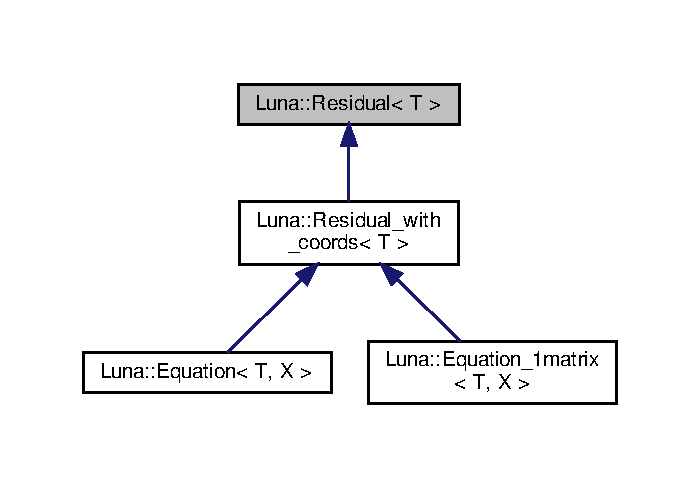
\includegraphics[width=336pt]{classLuna_1_1Residual__inherit__graph}
\end{center}
\end{figure}


Collaboration diagram for Luna\+:\+:Residual$<$ T $>$\+:\nopagebreak
\begin{figure}[H]
\begin{center}
\leavevmode
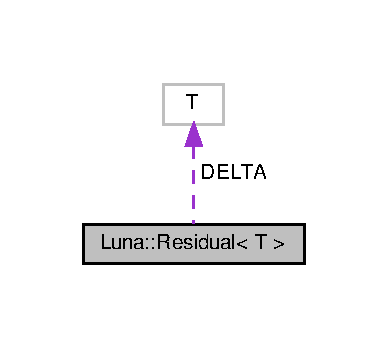
\includegraphics[width=186pt]{classLuna_1_1Residual__coll__graph}
\end{center}
\end{figure}
\subsection*{Public Member Functions}
\begin{DoxyCompactItemize}
\item 
\hyperlink{classLuna_1_1Residual_a6d918065d5ad8f65e5d226b9903af0cd}{Residual} (const unsigned \&order)
\begin{DoxyCompactList}\small\item\em Constructor for a \textquotesingle{}square\textquotesingle{} residual (N residuals for N unknowns) \end{DoxyCompactList}\item 
\hyperlink{classLuna_1_1Residual_a7c109fba68ee9658d4e2a81929c4c2cd}{Residual} (const unsigned \&order, const unsigned \&nvars)
\begin{DoxyCompactList}\small\item\em Constructor for a \textquotesingle{}non-\/square\textquotesingle{} residual object. \end{DoxyCompactList}\item 
virtual \hyperlink{classLuna_1_1Residual_a49919ce545464441f326d3be815241af}{$\sim$\+Residual} ()
\begin{DoxyCompactList}\small\item\em Destructor ( virtual since we have virtual functions ) \end{DoxyCompactList}\item 
unsigned \hyperlink{classLuna_1_1Residual_a866342c8d328177ea3f00c16d929cb0e}{get\+\_\+order} () const
\begin{DoxyCompactList}\small\item\em Get the order of the residual vector. \end{DoxyCompactList}\item 
unsigned \hyperlink{classLuna_1_1Residual_aa64479978dfc1879345e5b650881c488}{get\+\_\+number\+\_\+of\+\_\+vars} () const
\begin{DoxyCompactList}\small\item\em Get the number of variables. \end{DoxyCompactList}\item 
void \hyperlink{classLuna_1_1Residual_ac1f39e77c729e6a4a1e10ac951f6c704}{update} (const \hyperlink{classLuna_1_1Vector}{Vector}$<$ T $>$ \&\hyperlink{classLuna_1_1Residual_a41d9f863aa529f16c5d78fb19b4906bd}{state})
\begin{DoxyCompactList}\small\item\em Update the \hyperlink{classLuna_1_1Residual}{Residual} object for the current set of state variables. \end{DoxyCompactList}\item 
const \hyperlink{classLuna_1_1Vector}{Vector}$<$ T $>$ \& \hyperlink{classLuna_1_1Residual_a023ed8f4d0a5fa7acca0c982c746b662}{residual} () const
\begin{DoxyCompactList}\small\item\em A handle to the residuals corresponding to the last state. \end{DoxyCompactList}\item 
const \hyperlink{classLuna_1_1Matrix}{Matrix}$<$ T $>$ \& \hyperlink{classLuna_1_1Residual_adffbafa712fc6318f3cd05c03b88decb}{jacobian} () const
\begin{DoxyCompactList}\small\item\em A handle to the Jacobian of the residual. \end{DoxyCompactList}\item 
const \hyperlink{classLuna_1_1Vector}{Vector}$<$ T $>$ \& \hyperlink{classLuna_1_1Residual_a41d9f863aa529f16c5d78fb19b4906bd}{state} () const
\begin{DoxyCompactList}\small\item\em A handle to the state vector. \end{DoxyCompactList}\item 
T \& \hyperlink{classLuna_1_1Residual_a77c3f160a7683b9c960e5b3192107ae9}{delta} ()
\begin{DoxyCompactList}\small\item\em A handle to the step size used when finite-\/differencing. \end{DoxyCompactList}\item 
const T \& \hyperlink{classLuna_1_1Residual_a61c46d8d03274f949b2ac0832c30bde4}{delta} () const
\begin{DoxyCompactList}\small\item\em A handle to the step size used when finite-\/differencing. \end{DoxyCompactList}\item 
virtual void \hyperlink{classLuna_1_1Residual_ae1b1ebe3314c788b176bcac7b328de5c}{residual\+\_\+fn} (const \hyperlink{classLuna_1_1Vector}{Vector}$<$ T $>$ \&\hyperlink{classLuna_1_1Residual_a41d9f863aa529f16c5d78fb19b4906bd}{state}, \hyperlink{classLuna_1_1Vector}{Vector}$<$ T $>$ \&\hyperlink{Nonlinear__ODE__BVP_8cpp_a06fc87d81c62e9abb8790b6e5713c55ba7ce756344023b99e5ab27b804feb765c}{f}) const
\begin{DoxyCompactList}\small\item\em The residual function to be defined later. \end{DoxyCompactList}\end{DoxyCompactItemize}
\subsection*{Protected Member Functions}
\begin{DoxyCompactItemize}
\item 
virtual void \hyperlink{classLuna_1_1Residual_acfcbc7bc2731b0c432de7f98b9b7cca5}{jacobian} (const \hyperlink{classLuna_1_1Vector}{Vector}$<$ T $>$ \&\hyperlink{classLuna_1_1Residual_a41d9f863aa529f16c5d78fb19b4906bd}{state}, \hyperlink{classLuna_1_1Matrix}{Matrix}$<$ T $>$ \&jac) const
\begin{DoxyCompactList}\small\item\em Because the residual evaluation at the current state is assumed to have already been done by the \textquotesingle{}update\textquotesingle{} method, this routine is protected. \end{DoxyCompactList}\end{DoxyCompactItemize}
\subsection*{Protected Attributes}
\begin{DoxyCompactItemize}
\item 
\hyperlink{classLuna_1_1Matrix}{Matrix}$<$ T $>$ \hyperlink{classLuna_1_1Residual_ac76c460240288f84309b587c785df06a}{J\+A\+C\+\_\+\+A\+T\+\_\+\+L\+A\+S\+T\+\_\+\+S\+T\+A\+TE}
\item 
\hyperlink{classLuna_1_1Vector}{Vector}$<$ T $>$ \hyperlink{classLuna_1_1Residual_ac7b086911239d3f42ceec4a826e83543}{F\+N\+\_\+\+A\+T\+\_\+\+L\+A\+S\+T\+\_\+\+S\+T\+A\+TE}
\item 
\hyperlink{classLuna_1_1Vector}{Vector}$<$ T $>$ \hyperlink{classLuna_1_1Residual_abcfc99f00aa4cf3616b32dfd5315dece}{L\+A\+S\+T\+\_\+\+S\+T\+A\+TE}
\item 
T \hyperlink{classLuna_1_1Residual_a1bf38ddfa149797de560dcb11c975fef}{D\+E\+L\+TA}
\item 
unsigned \hyperlink{classLuna_1_1Residual_a7facf1267eb277d84aeea8beba2cb200}{O\+R\+D\+E\+R\+\_\+\+O\+F\+\_\+\+S\+Y\+S\+T\+EM}
\item 
unsigned \hyperlink{classLuna_1_1Residual_a8e7a52a94a49d900ba2784e621a35668}{N\+U\+M\+B\+E\+R\+\_\+\+O\+F\+\_\+\+V\+A\+RS}
\end{DoxyCompactItemize}


\subsection{Detailed Description}
\subsubsection*{template$<$class T$>$\newline
class Luna\+::\+Residual$<$ T $>$}

A templated base class to be inherited by objects that define residuals. 

Definition at line 22 of file Residual.\+h.



\subsection{Constructor \& Destructor Documentation}
\mbox{\Hypertarget{classLuna_1_1Residual_a6d918065d5ad8f65e5d226b9903af0cd}\label{classLuna_1_1Residual_a6d918065d5ad8f65e5d226b9903af0cd}} 
\index{Luna\+::\+Residual@{Luna\+::\+Residual}!Residual@{Residual}}
\index{Residual@{Residual}!Luna\+::\+Residual@{Luna\+::\+Residual}}
\subsubsection{\texorpdfstring{Residual()}{Residual()}\hspace{0.1cm}{\footnotesize\ttfamily [1/2]}}
{\footnotesize\ttfamily template$<$class T$>$ \\
\hyperlink{classLuna_1_1Residual}{Luna\+::\+Residual}$<$ T $>$\+::\hyperlink{classLuna_1_1Residual}{Residual} (\begin{DoxyParamCaption}\item[{const unsigned \&}]{order }\end{DoxyParamCaption})\hspace{0.3cm}{\ttfamily [inline]}}



Constructor for a \textquotesingle{}square\textquotesingle{} residual (N residuals for N unknowns) 


\begin{DoxyParams}{Parameters}
{\em order} & The order of the system of equations \\
\hline
\end{DoxyParams}


Definition at line 41 of file Residual.\+h.


\begin{DoxyCode}
41                                         : \hyperlink{classLuna_1_1Residual_a1bf38ddfa149797de560dcb11c975fef}{DELTA}( 1.e-8 )
42       \{
43         \hyperlink{classLuna_1_1Residual_a7facf1267eb277d84aeea8beba2cb200}{ORDER\_OF\_SYSTEM} = order;
44         \hyperlink{classLuna_1_1Residual_a8e7a52a94a49d900ba2784e621a35668}{NUMBER\_OF\_VARS} = order;
45         \hyperlink{classLuna_1_1Residual_abcfc99f00aa4cf3616b32dfd5315dece}{LAST\_STATE} = Vector<T>( \hyperlink{classLuna_1_1Residual_a8e7a52a94a49d900ba2784e621a35668}{NUMBER\_OF\_VARS}, 0.0 );
46         \hyperlink{classLuna_1_1Residual_ac7b086911239d3f42ceec4a826e83543}{FN\_AT\_LAST\_STATE} = Vector<T>( \hyperlink{classLuna_1_1Residual_a7facf1267eb277d84aeea8beba2cb200}{ORDER\_OF\_SYSTEM}, 0.0 );
47         \hyperlink{classLuna_1_1Residual_ac76c460240288f84309b587c785df06a}{JAC\_AT\_LAST\_STATE} = Matrix<T>( \hyperlink{classLuna_1_1Residual_a7facf1267eb277d84aeea8beba2cb200}{ORDER\_OF\_SYSTEM}, 
      \hyperlink{classLuna_1_1Residual_a8e7a52a94a49d900ba2784e621a35668}{NUMBER\_OF\_VARS}, 0.0 );
48       \}
\end{DoxyCode}
\mbox{\Hypertarget{classLuna_1_1Residual_a7c109fba68ee9658d4e2a81929c4c2cd}\label{classLuna_1_1Residual_a7c109fba68ee9658d4e2a81929c4c2cd}} 
\index{Luna\+::\+Residual@{Luna\+::\+Residual}!Residual@{Residual}}
\index{Residual@{Residual}!Luna\+::\+Residual@{Luna\+::\+Residual}}
\subsubsection{\texorpdfstring{Residual()}{Residual()}\hspace{0.1cm}{\footnotesize\ttfamily [2/2]}}
{\footnotesize\ttfamily template$<$class T$>$ \\
\hyperlink{classLuna_1_1Residual}{Luna\+::\+Residual}$<$ T $>$\+::\hyperlink{classLuna_1_1Residual}{Residual} (\begin{DoxyParamCaption}\item[{const unsigned \&}]{order,  }\item[{const unsigned \&}]{nvars }\end{DoxyParamCaption})\hspace{0.3cm}{\ttfamily [inline]}}



Constructor for a \textquotesingle{}non-\/square\textquotesingle{} residual object. 


\begin{DoxyParams}{Parameters}
{\em order} & The order of the system of equations \\
\hline
{\em nvars} & The number of elements in the state vector \\
\hline
\end{DoxyParams}


Definition at line 53 of file Residual.\+h.


\begin{DoxyCode}
54                                         : \hyperlink{classLuna_1_1Residual_a1bf38ddfa149797de560dcb11c975fef}{DELTA}( 1.e-8 )
55       \{
56         \hyperlink{classLuna_1_1Residual_a7facf1267eb277d84aeea8beba2cb200}{ORDER\_OF\_SYSTEM} = order;
57         \hyperlink{classLuna_1_1Residual_a8e7a52a94a49d900ba2784e621a35668}{NUMBER\_OF\_VARS} = nvars;
58         \hyperlink{classLuna_1_1Residual_abcfc99f00aa4cf3616b32dfd5315dece}{LAST\_STATE} = Vector<T>( \hyperlink{classLuna_1_1Residual_a8e7a52a94a49d900ba2784e621a35668}{NUMBER\_OF\_VARS}, 0.0 );
59         \hyperlink{classLuna_1_1Residual_ac7b086911239d3f42ceec4a826e83543}{FN\_AT\_LAST\_STATE} = Vector<T>( \hyperlink{classLuna_1_1Residual_a7facf1267eb277d84aeea8beba2cb200}{ORDER\_OF\_SYSTEM}, 0.0 );
60         \hyperlink{classLuna_1_1Residual_ac76c460240288f84309b587c785df06a}{JAC\_AT\_LAST\_STATE} = Matrix<T>( \hyperlink{classLuna_1_1Residual_a7facf1267eb277d84aeea8beba2cb200}{ORDER\_OF\_SYSTEM}, 
      \hyperlink{classLuna_1_1Residual_a8e7a52a94a49d900ba2784e621a35668}{NUMBER\_OF\_VARS}, 0.0 );
61       \}
\end{DoxyCode}
\mbox{\Hypertarget{classLuna_1_1Residual_a49919ce545464441f326d3be815241af}\label{classLuna_1_1Residual_a49919ce545464441f326d3be815241af}} 
\index{Luna\+::\+Residual@{Luna\+::\+Residual}!````~Residual@{$\sim$\+Residual}}
\index{````~Residual@{$\sim$\+Residual}!Luna\+::\+Residual@{Luna\+::\+Residual}}
\subsubsection{\texorpdfstring{$\sim$\+Residual()}{~Residual()}}
{\footnotesize\ttfamily template$<$class T$>$ \\
virtual \hyperlink{classLuna_1_1Residual}{Luna\+::\+Residual}$<$ T $>$\+::$\sim$\hyperlink{classLuna_1_1Residual}{Residual} (\begin{DoxyParamCaption}{ }\end{DoxyParamCaption})\hspace{0.3cm}{\ttfamily [inline]}, {\ttfamily [virtual]}}



Destructor ( virtual since we have virtual functions ) 



Definition at line 64 of file Residual.\+h.


\begin{DoxyCode}
65       \{\}
\end{DoxyCode}


\subsection{Member Function Documentation}
\mbox{\Hypertarget{classLuna_1_1Residual_a77c3f160a7683b9c960e5b3192107ae9}\label{classLuna_1_1Residual_a77c3f160a7683b9c960e5b3192107ae9}} 
\index{Luna\+::\+Residual@{Luna\+::\+Residual}!delta@{delta}}
\index{delta@{delta}!Luna\+::\+Residual@{Luna\+::\+Residual}}
\subsubsection{\texorpdfstring{delta()}{delta()}\hspace{0.1cm}{\footnotesize\ttfamily [1/2]}}
{\footnotesize\ttfamily template$<$class T$>$ \\
T\& \hyperlink{classLuna_1_1Residual}{Luna\+::\+Residual}$<$ T $>$\+::delta (\begin{DoxyParamCaption}{ }\end{DoxyParamCaption})\hspace{0.3cm}{\ttfamily [inline]}}



A handle to the step size used when finite-\/differencing. 

\begin{DoxyReturn}{Returns}
The step for FD computation of the Jacobian 
\end{DoxyReturn}


Definition at line 101 of file Residual.\+h.


\begin{DoxyCode}
101 \{ \textcolor{keywordflow}{return} \hyperlink{classLuna_1_1Residual_a1bf38ddfa149797de560dcb11c975fef}{DELTA}; \}
\end{DoxyCode}
\mbox{\Hypertarget{classLuna_1_1Residual_a61c46d8d03274f949b2ac0832c30bde4}\label{classLuna_1_1Residual_a61c46d8d03274f949b2ac0832c30bde4}} 
\index{Luna\+::\+Residual@{Luna\+::\+Residual}!delta@{delta}}
\index{delta@{delta}!Luna\+::\+Residual@{Luna\+::\+Residual}}
\subsubsection{\texorpdfstring{delta()}{delta()}\hspace{0.1cm}{\footnotesize\ttfamily [2/2]}}
{\footnotesize\ttfamily template$<$class T$>$ \\
const T\& \hyperlink{classLuna_1_1Residual}{Luna\+::\+Residual}$<$ T $>$\+::delta (\begin{DoxyParamCaption}{ }\end{DoxyParamCaption}) const\hspace{0.3cm}{\ttfamily [inline]}}



A handle to the step size used when finite-\/differencing. 

\begin{DoxyReturn}{Returns}
The step for FD computation of the Jacobian 
\end{DoxyReturn}


Definition at line 105 of file Residual.\+h.


\begin{DoxyCode}
105 \{ \textcolor{keywordflow}{return} \hyperlink{classLuna_1_1Residual_a1bf38ddfa149797de560dcb11c975fef}{DELTA}; \}
\end{DoxyCode}
\mbox{\Hypertarget{classLuna_1_1Residual_aa64479978dfc1879345e5b650881c488}\label{classLuna_1_1Residual_aa64479978dfc1879345e5b650881c488}} 
\index{Luna\+::\+Residual@{Luna\+::\+Residual}!get\+\_\+number\+\_\+of\+\_\+vars@{get\+\_\+number\+\_\+of\+\_\+vars}}
\index{get\+\_\+number\+\_\+of\+\_\+vars@{get\+\_\+number\+\_\+of\+\_\+vars}!Luna\+::\+Residual@{Luna\+::\+Residual}}
\subsubsection{\texorpdfstring{get\+\_\+number\+\_\+of\+\_\+vars()}{get\_number\_of\_vars()}}
{\footnotesize\ttfamily template$<$class T$>$ \\
unsigned \hyperlink{classLuna_1_1Residual}{Luna\+::\+Residual}$<$ T $>$\+::get\+\_\+number\+\_\+of\+\_\+vars (\begin{DoxyParamCaption}{ }\end{DoxyParamCaption}) const\hspace{0.3cm}{\ttfamily [inline]}}



Get the number of variables. 

\begin{DoxyReturn}{Returns}
The number of elements in the state vector 
\end{DoxyReturn}


Definition at line 76 of file Residual.\+h.


\begin{DoxyCode}
76 \{ \textcolor{keywordflow}{return} \hyperlink{classLuna_1_1Residual_a8e7a52a94a49d900ba2784e621a35668}{NUMBER\_OF\_VARS}; \}
\end{DoxyCode}
\mbox{\Hypertarget{classLuna_1_1Residual_a866342c8d328177ea3f00c16d929cb0e}\label{classLuna_1_1Residual_a866342c8d328177ea3f00c16d929cb0e}} 
\index{Luna\+::\+Residual@{Luna\+::\+Residual}!get\+\_\+order@{get\+\_\+order}}
\index{get\+\_\+order@{get\+\_\+order}!Luna\+::\+Residual@{Luna\+::\+Residual}}
\subsubsection{\texorpdfstring{get\+\_\+order()}{get\_order()}}
{\footnotesize\ttfamily template$<$class T$>$ \\
unsigned \hyperlink{classLuna_1_1Residual}{Luna\+::\+Residual}$<$ T $>$\+::get\+\_\+order (\begin{DoxyParamCaption}{ }\end{DoxyParamCaption}) const\hspace{0.3cm}{\ttfamily [inline]}}



Get the order of the residual vector. 

\begin{DoxyReturn}{Returns}
The order of the system of equations 
\end{DoxyReturn}


Definition at line 72 of file Residual.\+h.


\begin{DoxyCode}
72 \{ \textcolor{keywordflow}{return} \hyperlink{classLuna_1_1Residual_a7facf1267eb277d84aeea8beba2cb200}{ORDER\_OF\_SYSTEM}; \}
\end{DoxyCode}
\mbox{\Hypertarget{classLuna_1_1Residual_acfcbc7bc2731b0c432de7f98b9b7cca5}\label{classLuna_1_1Residual_acfcbc7bc2731b0c432de7f98b9b7cca5}} 
\index{Luna\+::\+Residual@{Luna\+::\+Residual}!jacobian@{jacobian}}
\index{jacobian@{jacobian}!Luna\+::\+Residual@{Luna\+::\+Residual}}
\subsubsection{\texorpdfstring{jacobian()}{jacobian()}\hspace{0.1cm}{\footnotesize\ttfamily [1/2]}}
{\footnotesize\ttfamily template$<$typename T$>$ \\
void \hyperlink{classLuna_1_1Residual}{Luna\+::\+Residual}$<$ T $>$\+::jacobian (\begin{DoxyParamCaption}\item[{const \hyperlink{classLuna_1_1Vector}{Vector}$<$ T $>$ \&}]{state,  }\item[{\hyperlink{classLuna_1_1Matrix}{Matrix}$<$ T $>$ \&}]{jac }\end{DoxyParamCaption}) const\hspace{0.3cm}{\ttfamily [inline]}, {\ttfamily [protected]}, {\ttfamily [virtual]}}



Because the residual evaluation at the current state is assumed to have already been done by the \textquotesingle{}update\textquotesingle{} method, this routine is protected. 

This default uses a finite-\/differenced Jacobian. You can overload this to provide an analytic Jacobian if you wish 

Definition at line 121 of file Residual.\+h.


\begin{DoxyCode}
123   \{
124     Vector<T> new\_state( \hyperlink{classLuna_1_1Residual_a41d9f863aa529f16c5d78fb19b4906bd}{state} );
125     \textcolor{comment}{// evaluation of the function}
126     Vector<T> f\_at\_new\_state( \hyperlink{classLuna_1_1Residual_a7facf1267eb277d84aeea8beba2cb200}{ORDER\_OF\_SYSTEM}, 0.0 );
127     \textcolor{comment}{// default is to FD the Jacobian}
128     \textcolor{keywordflow}{for} ( std::size\_t i = 0; i < \hyperlink{classLuna_1_1Residual_a8e7a52a94a49d900ba2784e621a35668}{NUMBER\_OF\_VARS}; ++i )
129     \{
130       new\_state[ i ] += \hyperlink{classLuna_1_1Residual_a1bf38ddfa149797de560dcb11c975fef}{DELTA};
131       \hyperlink{classLuna_1_1Residual_ae1b1ebe3314c788b176bcac7b328de5c}{residual\_fn}( new\_state, f\_at\_new\_state );
132       new\_state[ i ] -= \hyperlink{classLuna_1_1Residual_a1bf38ddfa149797de560dcb11c975fef}{DELTA};
133       jac.set\_col( i, ( f\_at\_new\_state - \hyperlink{classLuna_1_1Residual_ac7b086911239d3f42ceec4a826e83543}{FN\_AT\_LAST\_STATE} ) / 
      \hyperlink{classLuna_1_1Residual_a1bf38ddfa149797de560dcb11c975fef}{DELTA} );
134     \}
135   \}
\end{DoxyCode}
\mbox{\Hypertarget{classLuna_1_1Residual_adffbafa712fc6318f3cd05c03b88decb}\label{classLuna_1_1Residual_adffbafa712fc6318f3cd05c03b88decb}} 
\index{Luna\+::\+Residual@{Luna\+::\+Residual}!jacobian@{jacobian}}
\index{jacobian@{jacobian}!Luna\+::\+Residual@{Luna\+::\+Residual}}
\subsubsection{\texorpdfstring{jacobian()}{jacobian()}\hspace{0.1cm}{\footnotesize\ttfamily [2/2]}}
{\footnotesize\ttfamily template$<$class T$>$ \\
const \hyperlink{classLuna_1_1Matrix}{Matrix}$<$T$>$\& \hyperlink{classLuna_1_1Residual}{Luna\+::\+Residual}$<$ T $>$\+::jacobian (\begin{DoxyParamCaption}{ }\end{DoxyParamCaption}) const\hspace{0.3cm}{\ttfamily [inline]}}



A handle to the Jacobian of the residual. 

\begin{DoxyReturn}{Returns}
Jacobian for the last state vector 
\end{DoxyReturn}


Definition at line 93 of file Residual.\+h.



Referenced by Luna\+::\+Residual$<$ double $>$\+::update().


\begin{DoxyCode}
93 \{ \textcolor{keywordflow}{return} \hyperlink{classLuna_1_1Residual_ac76c460240288f84309b587c785df06a}{JAC\_AT\_LAST\_STATE}; \}
\end{DoxyCode}
\mbox{\Hypertarget{classLuna_1_1Residual_a023ed8f4d0a5fa7acca0c982c746b662}\label{classLuna_1_1Residual_a023ed8f4d0a5fa7acca0c982c746b662}} 
\index{Luna\+::\+Residual@{Luna\+::\+Residual}!residual@{residual}}
\index{residual@{residual}!Luna\+::\+Residual@{Luna\+::\+Residual}}
\subsubsection{\texorpdfstring{residual()}{residual()}}
{\footnotesize\ttfamily template$<$class T$>$ \\
const \hyperlink{classLuna_1_1Vector}{Vector}$<$T$>$\& \hyperlink{classLuna_1_1Residual}{Luna\+::\+Residual}$<$ T $>$\+::residual (\begin{DoxyParamCaption}{ }\end{DoxyParamCaption}) const\hspace{0.3cm}{\ttfamily [inline]}}



A handle to the residuals corresponding to the last state. 

\begin{DoxyReturn}{Returns}
\hyperlink{classLuna_1_1Residual}{Residual} for the last state vector 
\end{DoxyReturn}


Definition at line 89 of file Residual.\+h.


\begin{DoxyCode}
89 \{ \textcolor{keywordflow}{return} \hyperlink{classLuna_1_1Residual_ac7b086911239d3f42ceec4a826e83543}{FN\_AT\_LAST\_STATE}; \}
\end{DoxyCode}
\mbox{\Hypertarget{classLuna_1_1Residual_ae1b1ebe3314c788b176bcac7b328de5c}\label{classLuna_1_1Residual_ae1b1ebe3314c788b176bcac7b328de5c}} 
\index{Luna\+::\+Residual@{Luna\+::\+Residual}!residual\+\_\+fn@{residual\+\_\+fn}}
\index{residual\+\_\+fn@{residual\+\_\+fn}!Luna\+::\+Residual@{Luna\+::\+Residual}}
\subsubsection{\texorpdfstring{residual\+\_\+fn()}{residual\_fn()}}
{\footnotesize\ttfamily template$<$class T$>$ \\
virtual void \hyperlink{classLuna_1_1Residual}{Luna\+::\+Residual}$<$ T $>$\+::residual\+\_\+fn (\begin{DoxyParamCaption}\item[{const \hyperlink{classLuna_1_1Vector}{Vector}$<$ T $>$ \&}]{state,  }\item[{\hyperlink{classLuna_1_1Vector}{Vector}$<$ T $>$ \&}]{f }\end{DoxyParamCaption}) const\hspace{0.3cm}{\ttfamily [inline]}, {\ttfamily [virtual]}}



The residual function to be defined later. 


\begin{DoxyParams}{Parameters}
{\em state} & The current state \hyperlink{classLuna_1_1Vector}{Vector} \\
\hline
{\em f} & The function \hyperlink{classLuna_1_1Vector}{Vector} to be updated \\
\hline
\end{DoxyParams}


Reimplemented in \hyperlink{classLuna_1_1right__BC_a513bb865a218a9ee309727839496afe0}{Luna\+::right\+\_\+\+BC}, \hyperlink{classLuna_1_1right__BC_a513bb865a218a9ee309727839496afe0}{Luna\+::right\+\_\+\+BC}, \hyperlink{classLuna_1_1left__BC_a01645de89a78c7c925d60bb68e994c90}{Luna\+::left\+\_\+\+BC}, \hyperlink{classLuna_1_1left__BC_a01645de89a78c7c925d60bb68e994c90}{Luna\+::left\+\_\+\+BC}, \hyperlink{classLuna_1_1Arc__problem_aeb5e14b8b06d0ad0f8b42cb280836f97}{Luna\+::\+Arc\+\_\+problem}, \hyperlink{classLuna_1_1nonlinear__equation_a5acffbdc83b8b487241cd92b0191be85}{Luna\+::nonlinear\+\_\+equation}, \hyperlink{classLuna_1_1test__equation_a90a4576ce51729e49dbe67f36ab31f81}{Luna\+::test\+\_\+equation}, and \hyperlink{classLuna_1_1test__residual_abf5e77702d2ffec8bf2ffdc6728a8473}{Luna\+::test\+\_\+residual}.



Definition at line 110 of file Residual.\+h.



Referenced by Luna\+::\+Residual$<$ double $>$\+::jacobian(), and Luna\+::\+Residual$<$ double $>$\+::update().


\begin{DoxyCode}
111       \{
112         std::string problem;
113         problem = \textcolor{stringliteral}{"The residual\_fn method has not been implemented.\(\backslash\)n"};
114         problem += \textcolor{stringliteral}{"You must implement this method to define the residual.\(\backslash\)n"};
115         \textcolor{keywordflow}{throw} Error( problem );
116       \}
\end{DoxyCode}
\mbox{\Hypertarget{classLuna_1_1Residual_a41d9f863aa529f16c5d78fb19b4906bd}\label{classLuna_1_1Residual_a41d9f863aa529f16c5d78fb19b4906bd}} 
\index{Luna\+::\+Residual@{Luna\+::\+Residual}!state@{state}}
\index{state@{state}!Luna\+::\+Residual@{Luna\+::\+Residual}}
\subsubsection{\texorpdfstring{state()}{state()}}
{\footnotesize\ttfamily template$<$class T$>$ \\
const \hyperlink{classLuna_1_1Vector}{Vector}$<$T$>$\& \hyperlink{classLuna_1_1Residual}{Luna\+::\+Residual}$<$ T $>$\+::state (\begin{DoxyParamCaption}{ }\end{DoxyParamCaption}) const\hspace{0.3cm}{\ttfamily [inline]}}



A handle to the state vector. 

\begin{DoxyReturn}{Returns}
The last state vector 
\end{DoxyReturn}


Definition at line 97 of file Residual.\+h.



Referenced by Luna\+::\+Residual$<$ double $>$\+::update().


\begin{DoxyCode}
97 \{ \textcolor{keywordflow}{return} \hyperlink{classLuna_1_1Residual_abcfc99f00aa4cf3616b32dfd5315dece}{LAST\_STATE}; \}
\end{DoxyCode}
\mbox{\Hypertarget{classLuna_1_1Residual_ac1f39e77c729e6a4a1e10ac951f6c704}\label{classLuna_1_1Residual_ac1f39e77c729e6a4a1e10ac951f6c704}} 
\index{Luna\+::\+Residual@{Luna\+::\+Residual}!update@{update}}
\index{update@{update}!Luna\+::\+Residual@{Luna\+::\+Residual}}
\subsubsection{\texorpdfstring{update()}{update()}}
{\footnotesize\ttfamily template$<$class T$>$ \\
void \hyperlink{classLuna_1_1Residual}{Luna\+::\+Residual}$<$ T $>$\+::update (\begin{DoxyParamCaption}\item[{const \hyperlink{classLuna_1_1Vector}{Vector}$<$ T $>$ \&}]{state }\end{DoxyParamCaption})\hspace{0.3cm}{\ttfamily [inline]}}



Update the \hyperlink{classLuna_1_1Residual}{Residual} object for the current set of state variables. 


\begin{DoxyParams}{Parameters}
{\em The} & last state vector \\
\hline
\end{DoxyParams}


Definition at line 80 of file Residual.\+h.


\begin{DoxyCode}
81       \{
82         \hyperlink{classLuna_1_1Residual_abcfc99f00aa4cf3616b32dfd5315dece}{LAST\_STATE} = \hyperlink{classLuna_1_1Residual_a41d9f863aa529f16c5d78fb19b4906bd}{state};
83         \hyperlink{classLuna_1_1Residual_ae1b1ebe3314c788b176bcac7b328de5c}{residual\_fn}( \hyperlink{classLuna_1_1Residual_abcfc99f00aa4cf3616b32dfd5315dece}{LAST\_STATE}, \hyperlink{classLuna_1_1Residual_ac7b086911239d3f42ceec4a826e83543}{FN\_AT\_LAST\_STATE} );
84         \hyperlink{classLuna_1_1Residual_adffbafa712fc6318f3cd05c03b88decb}{jacobian}( \hyperlink{classLuna_1_1Residual_abcfc99f00aa4cf3616b32dfd5315dece}{LAST\_STATE}, \hyperlink{classLuna_1_1Residual_ac76c460240288f84309b587c785df06a}{JAC\_AT\_LAST\_STATE} );
85       \}
\end{DoxyCode}


\subsection{Member Data Documentation}
\mbox{\Hypertarget{classLuna_1_1Residual_a1bf38ddfa149797de560dcb11c975fef}\label{classLuna_1_1Residual_a1bf38ddfa149797de560dcb11c975fef}} 
\index{Luna\+::\+Residual@{Luna\+::\+Residual}!D\+E\+L\+TA@{D\+E\+L\+TA}}
\index{D\+E\+L\+TA@{D\+E\+L\+TA}!Luna\+::\+Residual@{Luna\+::\+Residual}}
\subsubsection{\texorpdfstring{D\+E\+L\+TA}{DELTA}}
{\footnotesize\ttfamily template$<$class T$>$ \\
T \hyperlink{classLuna_1_1Residual}{Luna\+::\+Residual}$<$ T $>$\+::D\+E\+L\+TA\hspace{0.3cm}{\ttfamily [protected]}}



Definition at line 34 of file Residual.\+h.



Referenced by Luna\+::\+Residual$<$ double $>$\+::delta(), and Luna\+::\+Residual$<$ double $>$\+::jacobian().

\mbox{\Hypertarget{classLuna_1_1Residual_ac7b086911239d3f42ceec4a826e83543}\label{classLuna_1_1Residual_ac7b086911239d3f42ceec4a826e83543}} 
\index{Luna\+::\+Residual@{Luna\+::\+Residual}!F\+N\+\_\+\+A\+T\+\_\+\+L\+A\+S\+T\+\_\+\+S\+T\+A\+TE@{F\+N\+\_\+\+A\+T\+\_\+\+L\+A\+S\+T\+\_\+\+S\+T\+A\+TE}}
\index{F\+N\+\_\+\+A\+T\+\_\+\+L\+A\+S\+T\+\_\+\+S\+T\+A\+TE@{F\+N\+\_\+\+A\+T\+\_\+\+L\+A\+S\+T\+\_\+\+S\+T\+A\+TE}!Luna\+::\+Residual@{Luna\+::\+Residual}}
\subsubsection{\texorpdfstring{F\+N\+\_\+\+A\+T\+\_\+\+L\+A\+S\+T\+\_\+\+S\+T\+A\+TE}{FN\_AT\_LAST\_STATE}}
{\footnotesize\ttfamily template$<$class T$>$ \\
\hyperlink{classLuna_1_1Vector}{Vector}$<$T$>$ \hyperlink{classLuna_1_1Residual}{Luna\+::\+Residual}$<$ T $>$\+::F\+N\+\_\+\+A\+T\+\_\+\+L\+A\+S\+T\+\_\+\+S\+T\+A\+TE\hspace{0.3cm}{\ttfamily [protected]}}



Definition at line 32 of file Residual.\+h.



Referenced by Luna\+::\+Residual$<$ double $>$\+::jacobian(), and Luna\+::\+Residual$<$ double $>$\+::residual().

\mbox{\Hypertarget{classLuna_1_1Residual_ac76c460240288f84309b587c785df06a}\label{classLuna_1_1Residual_ac76c460240288f84309b587c785df06a}} 
\index{Luna\+::\+Residual@{Luna\+::\+Residual}!J\+A\+C\+\_\+\+A\+T\+\_\+\+L\+A\+S\+T\+\_\+\+S\+T\+A\+TE@{J\+A\+C\+\_\+\+A\+T\+\_\+\+L\+A\+S\+T\+\_\+\+S\+T\+A\+TE}}
\index{J\+A\+C\+\_\+\+A\+T\+\_\+\+L\+A\+S\+T\+\_\+\+S\+T\+A\+TE@{J\+A\+C\+\_\+\+A\+T\+\_\+\+L\+A\+S\+T\+\_\+\+S\+T\+A\+TE}!Luna\+::\+Residual@{Luna\+::\+Residual}}
\subsubsection{\texorpdfstring{J\+A\+C\+\_\+\+A\+T\+\_\+\+L\+A\+S\+T\+\_\+\+S\+T\+A\+TE}{JAC\_AT\_LAST\_STATE}}
{\footnotesize\ttfamily template$<$class T$>$ \\
\hyperlink{classLuna_1_1Matrix}{Matrix}$<$T$>$ \hyperlink{classLuna_1_1Residual}{Luna\+::\+Residual}$<$ T $>$\+::J\+A\+C\+\_\+\+A\+T\+\_\+\+L\+A\+S\+T\+\_\+\+S\+T\+A\+TE\hspace{0.3cm}{\ttfamily [protected]}}



Definition at line 31 of file Residual.\+h.



Referenced by Luna\+::\+Residual$<$ double $>$\+::jacobian().

\mbox{\Hypertarget{classLuna_1_1Residual_abcfc99f00aa4cf3616b32dfd5315dece}\label{classLuna_1_1Residual_abcfc99f00aa4cf3616b32dfd5315dece}} 
\index{Luna\+::\+Residual@{Luna\+::\+Residual}!L\+A\+S\+T\+\_\+\+S\+T\+A\+TE@{L\+A\+S\+T\+\_\+\+S\+T\+A\+TE}}
\index{L\+A\+S\+T\+\_\+\+S\+T\+A\+TE@{L\+A\+S\+T\+\_\+\+S\+T\+A\+TE}!Luna\+::\+Residual@{Luna\+::\+Residual}}
\subsubsection{\texorpdfstring{L\+A\+S\+T\+\_\+\+S\+T\+A\+TE}{LAST\_STATE}}
{\footnotesize\ttfamily template$<$class T$>$ \\
\hyperlink{classLuna_1_1Vector}{Vector}$<$T$>$ \hyperlink{classLuna_1_1Residual}{Luna\+::\+Residual}$<$ T $>$\+::L\+A\+S\+T\+\_\+\+S\+T\+A\+TE\hspace{0.3cm}{\ttfamily [protected]}}



Definition at line 33 of file Residual.\+h.



Referenced by Luna\+::\+Residual$<$ double $>$\+::state().

\mbox{\Hypertarget{classLuna_1_1Residual_a8e7a52a94a49d900ba2784e621a35668}\label{classLuna_1_1Residual_a8e7a52a94a49d900ba2784e621a35668}} 
\index{Luna\+::\+Residual@{Luna\+::\+Residual}!N\+U\+M\+B\+E\+R\+\_\+\+O\+F\+\_\+\+V\+A\+RS@{N\+U\+M\+B\+E\+R\+\_\+\+O\+F\+\_\+\+V\+A\+RS}}
\index{N\+U\+M\+B\+E\+R\+\_\+\+O\+F\+\_\+\+V\+A\+RS@{N\+U\+M\+B\+E\+R\+\_\+\+O\+F\+\_\+\+V\+A\+RS}!Luna\+::\+Residual@{Luna\+::\+Residual}}
\subsubsection{\texorpdfstring{N\+U\+M\+B\+E\+R\+\_\+\+O\+F\+\_\+\+V\+A\+RS}{NUMBER\_OF\_VARS}}
{\footnotesize\ttfamily template$<$class T$>$ \\
unsigned \hyperlink{classLuna_1_1Residual}{Luna\+::\+Residual}$<$ T $>$\+::N\+U\+M\+B\+E\+R\+\_\+\+O\+F\+\_\+\+V\+A\+RS\hspace{0.3cm}{\ttfamily [protected]}}



Definition at line 36 of file Residual.\+h.



Referenced by Luna\+::\+Residual$<$ double $>$\+::get\+\_\+number\+\_\+of\+\_\+vars(), Luna\+::\+Residual$<$ double $>$\+::jacobian(), and Luna\+::\+Residual$<$ double $>$\+::\+Residual().

\mbox{\Hypertarget{classLuna_1_1Residual_a7facf1267eb277d84aeea8beba2cb200}\label{classLuna_1_1Residual_a7facf1267eb277d84aeea8beba2cb200}} 
\index{Luna\+::\+Residual@{Luna\+::\+Residual}!O\+R\+D\+E\+R\+\_\+\+O\+F\+\_\+\+S\+Y\+S\+T\+EM@{O\+R\+D\+E\+R\+\_\+\+O\+F\+\_\+\+S\+Y\+S\+T\+EM}}
\index{O\+R\+D\+E\+R\+\_\+\+O\+F\+\_\+\+S\+Y\+S\+T\+EM@{O\+R\+D\+E\+R\+\_\+\+O\+F\+\_\+\+S\+Y\+S\+T\+EM}!Luna\+::\+Residual@{Luna\+::\+Residual}}
\subsubsection{\texorpdfstring{O\+R\+D\+E\+R\+\_\+\+O\+F\+\_\+\+S\+Y\+S\+T\+EM}{ORDER\_OF\_SYSTEM}}
{\footnotesize\ttfamily template$<$class T$>$ \\
unsigned \hyperlink{classLuna_1_1Residual}{Luna\+::\+Residual}$<$ T $>$\+::O\+R\+D\+E\+R\+\_\+\+O\+F\+\_\+\+S\+Y\+S\+T\+EM\hspace{0.3cm}{\ttfamily [protected]}}



Definition at line 35 of file Residual.\+h.



Referenced by Luna\+::\+Residual$<$ double $>$\+::get\+\_\+order(), Luna\+::\+Residual$<$ double $>$\+::jacobian(), and Luna\+::\+Residual$<$ double $>$\+::\+Residual().



The documentation for this class was generated from the following file\+:\begin{DoxyCompactItemize}
\item 
include/\+Luna/\hyperlink{Residual_8h}{Residual.\+h}\end{DoxyCompactItemize}

\hypertarget{classLuna_1_1Residual__with__coords}{}\section{Luna\+:\+:Residual\+\_\+with\+\_\+coords$<$ T, X $>$ Class Template Reference}
\label{classLuna_1_1Residual__with__coords}\index{Luna\+::\+Residual\+\_\+with\+\_\+coords$<$ T, X $>$@{Luna\+::\+Residual\+\_\+with\+\_\+coords$<$ T, X $>$}}


{\ttfamily \#include $<$Residual\+\_\+with\+\_\+coords.\+h$>$}



Inheritance diagram for Luna\+:\+:Residual\+\_\+with\+\_\+coords$<$ T, X $>$\+:\nopagebreak
\begin{figure}[H]
\begin{center}
\leavevmode
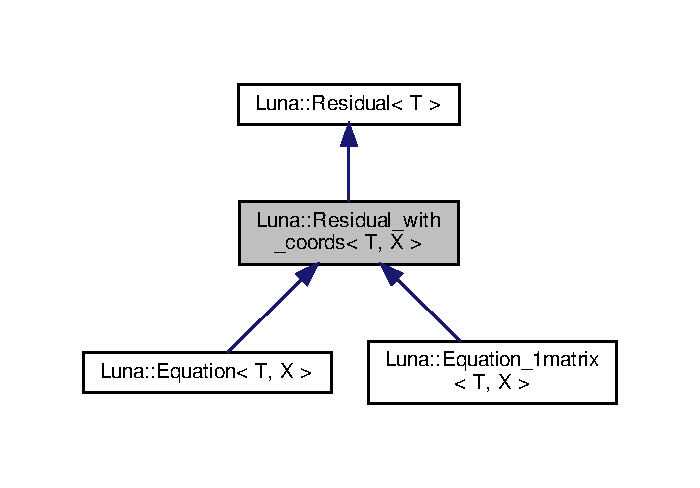
\includegraphics[width=336pt]{classLuna_1_1Residual__with__coords__inherit__graph}
\end{center}
\end{figure}


Collaboration diagram for Luna\+:\+:Residual\+\_\+with\+\_\+coords$<$ T, X $>$\+:\nopagebreak
\begin{figure}[H]
\begin{center}
\leavevmode
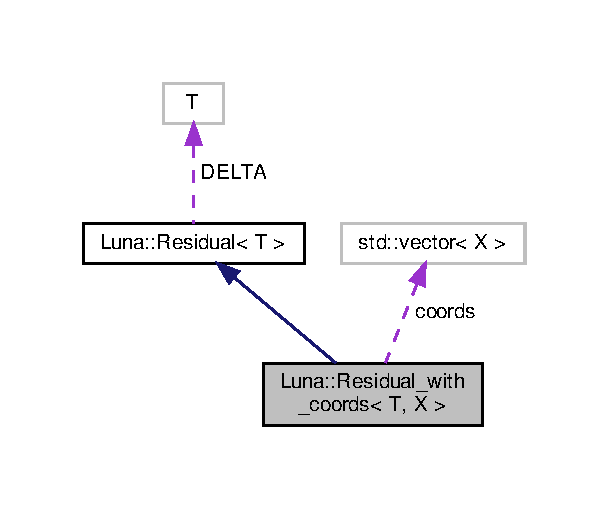
\includegraphics[width=292pt]{classLuna_1_1Residual__with__coords__coll__graph}
\end{center}
\end{figure}
\subsection*{Public Member Functions}
\begin{DoxyCompactItemize}
\item 
\hyperlink{classLuna_1_1Residual__with__coords_a61285d7e42d5ec57ba479e725cfd0340}{Residual\+\_\+with\+\_\+coords} (const unsigned \&order, const unsigned \&ncoords)
\begin{DoxyCompactList}\small\item\em Constructor for a square residual object, N residuals for N unknowns. \end{DoxyCompactList}\item 
\hyperlink{classLuna_1_1Residual__with__coords_aae68175ceb4157780d225d5e3d52bbbf}{Residual\+\_\+with\+\_\+coords} (const unsigned \&order, const unsigned \&nvars, const unsigned \&ncoords)
\begin{DoxyCompactList}\small\item\em Constructor for a non-\/square residual object, there are less residual constraints than unknowns. \end{DoxyCompactList}\item 
virtual \hyperlink{classLuna_1_1Residual__with__coords_ac10681ab24e23a4eabeb42f2001887d1}{$\sim$\+Residual\+\_\+with\+\_\+coords} ()
\begin{DoxyCompactList}\small\item\em An empty destructor. \end{DoxyCompactList}\item 
X \& \hyperlink{classLuna_1_1Residual__with__coords_a3fa4c950a944743c0380e4c151728372}{coord} (const unsigned \&i)
\begin{DoxyCompactList}\small\item\em General handle access to the coordinates. \end{DoxyCompactList}\item 
const X \& \hyperlink{classLuna_1_1Residual__with__coords_a6fca44ee46cbe0fee796f3d0cf43f74e}{coord} (const unsigned \&i) const
\begin{DoxyCompactList}\small\item\em General handle access to the coordinates. \end{DoxyCompactList}\end{DoxyCompactItemize}
\subsection*{Protected Attributes}
\begin{DoxyCompactItemize}
\item 
std\+::vector$<$ X $>$ \hyperlink{classLuna_1_1Residual__with__coords_a3f69e7026c7f86e14bc94ededc86ee62}{coords}
\begin{DoxyCompactList}\small\item\em The coordinates stored for this residual. \end{DoxyCompactList}\end{DoxyCompactItemize}
\subsection*{Additional Inherited Members}


\subsection{Detailed Description}
\subsubsection*{template$<$class T, class X = double$>$\newline
class Luna\+::\+Residual\+\_\+with\+\_\+coords$<$ T, X $>$}



Definition at line 19 of file Residual\+\_\+with\+\_\+coords.\+h.



\subsection{Constructor \& Destructor Documentation}
\mbox{\Hypertarget{classLuna_1_1Residual__with__coords_a61285d7e42d5ec57ba479e725cfd0340}\label{classLuna_1_1Residual__with__coords_a61285d7e42d5ec57ba479e725cfd0340}} 
\index{Luna\+::\+Residual\+\_\+with\+\_\+coords@{Luna\+::\+Residual\+\_\+with\+\_\+coords}!Residual\+\_\+with\+\_\+coords@{Residual\+\_\+with\+\_\+coords}}
\index{Residual\+\_\+with\+\_\+coords@{Residual\+\_\+with\+\_\+coords}!Luna\+::\+Residual\+\_\+with\+\_\+coords@{Luna\+::\+Residual\+\_\+with\+\_\+coords}}
\subsubsection{\texorpdfstring{Residual\+\_\+with\+\_\+coords()}{Residual\_with\_coords()}\hspace{0.1cm}{\footnotesize\ttfamily [1/2]}}
{\footnotesize\ttfamily template$<$typename T , typename X $>$ \\
\hyperlink{classLuna_1_1Residual__with__coords}{Luna\+::\+Residual\+\_\+with\+\_\+coords}$<$ T, X $>$\+::\hyperlink{classLuna_1_1Residual__with__coords}{Residual\+\_\+with\+\_\+coords} (\begin{DoxyParamCaption}\item[{const unsigned \&}]{order,  }\item[{const unsigned \&}]{ncoords }\end{DoxyParamCaption})}



Constructor for a square residual object, N residuals for N unknowns. 


\begin{DoxyParams}{Parameters}
{\em order} & The order of the residual vector \\
\hline
{\em ncoords} & The number of coordinates to store \\
\hline
\end{DoxyParams}


Definition at line 54 of file Residual\+\_\+with\+\_\+coords.\+h.


\begin{DoxyCode}
55                                                         : Residual<T>( order )
56   \{
57     \hyperlink{classLuna_1_1Residual__with__coords_a3f69e7026c7f86e14bc94ededc86ee62}{coords} = std::vector<X>( ncoords, 0.0 );
58   \}
\end{DoxyCode}
\mbox{\Hypertarget{classLuna_1_1Residual__with__coords_aae68175ceb4157780d225d5e3d52bbbf}\label{classLuna_1_1Residual__with__coords_aae68175ceb4157780d225d5e3d52bbbf}} 
\index{Luna\+::\+Residual\+\_\+with\+\_\+coords@{Luna\+::\+Residual\+\_\+with\+\_\+coords}!Residual\+\_\+with\+\_\+coords@{Residual\+\_\+with\+\_\+coords}}
\index{Residual\+\_\+with\+\_\+coords@{Residual\+\_\+with\+\_\+coords}!Luna\+::\+Residual\+\_\+with\+\_\+coords@{Luna\+::\+Residual\+\_\+with\+\_\+coords}}
\subsubsection{\texorpdfstring{Residual\+\_\+with\+\_\+coords()}{Residual\_with\_coords()}\hspace{0.1cm}{\footnotesize\ttfamily [2/2]}}
{\footnotesize\ttfamily template$<$typename T , typename X $>$ \\
\hyperlink{classLuna_1_1Residual__with__coords}{Luna\+::\+Residual\+\_\+with\+\_\+coords}$<$ T, X $>$\+::\hyperlink{classLuna_1_1Residual__with__coords}{Residual\+\_\+with\+\_\+coords} (\begin{DoxyParamCaption}\item[{const unsigned \&}]{order,  }\item[{const unsigned \&}]{nvars,  }\item[{const unsigned \&}]{ncoords }\end{DoxyParamCaption})}



Constructor for a non-\/square residual object, there are less residual constraints than unknowns. 


\begin{DoxyParams}{Parameters}
{\em order} & The number of residuals \\
\hline
{\em nvars} & The number of unknowns/variables \\
\hline
{\em ncoords} & The number of coordinates to store \\
\hline
\end{DoxyParams}


Definition at line 61 of file Residual\+\_\+with\+\_\+coords.\+h.


\begin{DoxyCode}
63                                                   : Residual<T>( order, nvars )
64   \{
65     \hyperlink{classLuna_1_1Residual__with__coords_a3f69e7026c7f86e14bc94ededc86ee62}{coords} = std::vector<X>( ncoords, 0.0 );
66   \}
\end{DoxyCode}
\mbox{\Hypertarget{classLuna_1_1Residual__with__coords_ac10681ab24e23a4eabeb42f2001887d1}\label{classLuna_1_1Residual__with__coords_ac10681ab24e23a4eabeb42f2001887d1}} 
\index{Luna\+::\+Residual\+\_\+with\+\_\+coords@{Luna\+::\+Residual\+\_\+with\+\_\+coords}!````~Residual\+\_\+with\+\_\+coords@{$\sim$\+Residual\+\_\+with\+\_\+coords}}
\index{````~Residual\+\_\+with\+\_\+coords@{$\sim$\+Residual\+\_\+with\+\_\+coords}!Luna\+::\+Residual\+\_\+with\+\_\+coords@{Luna\+::\+Residual\+\_\+with\+\_\+coords}}
\subsubsection{\texorpdfstring{$\sim$\+Residual\+\_\+with\+\_\+coords()}{~Residual\_with\_coords()}}
{\footnotesize\ttfamily template$<$typename T , typename X $>$ \\
\hyperlink{classLuna_1_1Residual__with__coords}{Luna\+::\+Residual\+\_\+with\+\_\+coords}$<$ T, X $>$\+::$\sim$\hyperlink{classLuna_1_1Residual__with__coords}{Residual\+\_\+with\+\_\+coords} (\begin{DoxyParamCaption}{ }\end{DoxyParamCaption})\hspace{0.3cm}{\ttfamily [virtual]}}



An empty destructor. 



Definition at line 69 of file Residual\+\_\+with\+\_\+coords.\+h.


\begin{DoxyCode}
70   \{
71   \}
\end{DoxyCode}


\subsection{Member Function Documentation}
\mbox{\Hypertarget{classLuna_1_1Residual__with__coords_a3fa4c950a944743c0380e4c151728372}\label{classLuna_1_1Residual__with__coords_a3fa4c950a944743c0380e4c151728372}} 
\index{Luna\+::\+Residual\+\_\+with\+\_\+coords@{Luna\+::\+Residual\+\_\+with\+\_\+coords}!coord@{coord}}
\index{coord@{coord}!Luna\+::\+Residual\+\_\+with\+\_\+coords@{Luna\+::\+Residual\+\_\+with\+\_\+coords}}
\subsubsection{\texorpdfstring{coord()}{coord()}\hspace{0.1cm}{\footnotesize\ttfamily [1/2]}}
{\footnotesize\ttfamily template$<$typename T , typename X $>$ \\
X \& \hyperlink{classLuna_1_1Residual__with__coords}{Luna\+::\+Residual\+\_\+with\+\_\+coords}$<$ T, X $>$\+::coord (\begin{DoxyParamCaption}\item[{const unsigned \&}]{i }\end{DoxyParamCaption})\hspace{0.3cm}{\ttfamily [inline]}}



General handle access to the coordinates. 

\begin{DoxyReturn}{Returns}
A handle to the i-\/th coordinate 
\end{DoxyReturn}


Definition at line 74 of file Residual\+\_\+with\+\_\+coords.\+h.


\begin{DoxyCode}
75   \{
76     \textcolor{keywordflow}{return} \hyperlink{classLuna_1_1Residual__with__coords_a3f69e7026c7f86e14bc94ededc86ee62}{coords}[ i ];
77   \}
\end{DoxyCode}
\mbox{\Hypertarget{classLuna_1_1Residual__with__coords_a6fca44ee46cbe0fee796f3d0cf43f74e}\label{classLuna_1_1Residual__with__coords_a6fca44ee46cbe0fee796f3d0cf43f74e}} 
\index{Luna\+::\+Residual\+\_\+with\+\_\+coords@{Luna\+::\+Residual\+\_\+with\+\_\+coords}!coord@{coord}}
\index{coord@{coord}!Luna\+::\+Residual\+\_\+with\+\_\+coords@{Luna\+::\+Residual\+\_\+with\+\_\+coords}}
\subsubsection{\texorpdfstring{coord()}{coord()}\hspace{0.1cm}{\footnotesize\ttfamily [2/2]}}
{\footnotesize\ttfamily template$<$typename T , typename X $>$ \\
const X \& \hyperlink{classLuna_1_1Residual__with__coords}{Luna\+::\+Residual\+\_\+with\+\_\+coords}$<$ T, X $>$\+::coord (\begin{DoxyParamCaption}\item[{const unsigned \&}]{i }\end{DoxyParamCaption}) const\hspace{0.3cm}{\ttfamily [inline]}}



General handle access to the coordinates. 

\begin{DoxyReturn}{Returns}
A handle to the i-\/th coordinate 
\end{DoxyReturn}


Definition at line 80 of file Residual\+\_\+with\+\_\+coords.\+h.


\begin{DoxyCode}
81   \{
82     \textcolor{keywordflow}{return} \hyperlink{classLuna_1_1Residual__with__coords_a3f69e7026c7f86e14bc94ededc86ee62}{coords}[ i ];
83   \}
\end{DoxyCode}


\subsection{Member Data Documentation}
\mbox{\Hypertarget{classLuna_1_1Residual__with__coords_a3f69e7026c7f86e14bc94ededc86ee62}\label{classLuna_1_1Residual__with__coords_a3f69e7026c7f86e14bc94ededc86ee62}} 
\index{Luna\+::\+Residual\+\_\+with\+\_\+coords@{Luna\+::\+Residual\+\_\+with\+\_\+coords}!coords@{coords}}
\index{coords@{coords}!Luna\+::\+Residual\+\_\+with\+\_\+coords@{Luna\+::\+Residual\+\_\+with\+\_\+coords}}
\subsubsection{\texorpdfstring{coords}{coords}}
{\footnotesize\ttfamily template$<$class T, class X = double$>$ \\
std\+::vector$<$X$>$ \hyperlink{classLuna_1_1Residual__with__coords}{Luna\+::\+Residual\+\_\+with\+\_\+coords}$<$ T, X $>$\+::coords\hspace{0.3cm}{\ttfamily [protected]}}



The coordinates stored for this residual. 



Definition at line 49 of file Residual\+\_\+with\+\_\+coords.\+h.



The documentation for this class was generated from the following file\+:\begin{DoxyCompactItemize}
\item 
include/\+Luna/\hyperlink{Residual__with__coords_8h}{Residual\+\_\+with\+\_\+coords.\+h}\end{DoxyCompactItemize}

\hypertarget{classLuna_1_1right__BC}{}\section{Luna\+:\+:right\+\_\+\+BC Class Reference}
\label{classLuna_1_1right__BC}\index{Luna\+::right\+\_\+\+BC@{Luna\+::right\+\_\+\+BC}}


Inheritance diagram for Luna\+:\+:right\+\_\+\+BC\+:\nopagebreak
\begin{figure}[H]
\begin{center}
\leavevmode
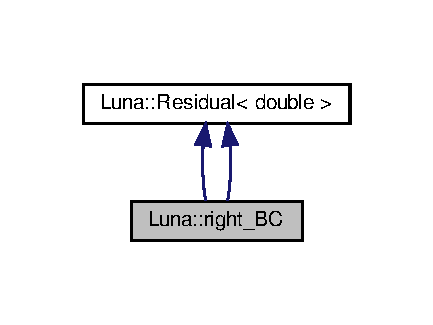
\includegraphics[width=208pt]{classLuna_1_1right__BC__inherit__graph}
\end{center}
\end{figure}


Collaboration diagram for Luna\+:\+:right\+\_\+\+BC\+:\nopagebreak
\begin{figure}[H]
\begin{center}
\leavevmode
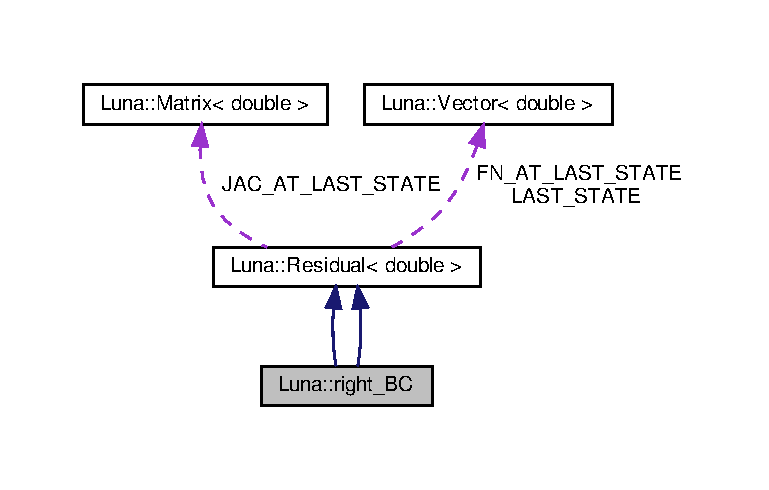
\includegraphics[width=350pt]{classLuna_1_1right__BC__coll__graph}
\end{center}
\end{figure}
\subsection*{Public Member Functions}
\begin{DoxyCompactItemize}
\item 
\hyperlink{classLuna_1_1right__BC_af63a57e305306468e26f7bdb5842e1e6}{right\+\_\+\+BC} ()
\item 
void \hyperlink{classLuna_1_1right__BC_a513bb865a218a9ee309727839496afe0}{residual\+\_\+fn} (const \hyperlink{classLuna_1_1Vector}{Vector}$<$ double $>$ \&z, \hyperlink{classLuna_1_1Vector}{Vector}$<$ double $>$ \&B) const
\begin{DoxyCompactList}\small\item\em The residual function to be defined later. \end{DoxyCompactList}\item 
\hyperlink{classLuna_1_1right__BC_af63a57e305306468e26f7bdb5842e1e6}{right\+\_\+\+BC} ()
\item 
void \hyperlink{classLuna_1_1right__BC_a513bb865a218a9ee309727839496afe0}{residual\+\_\+fn} (const \hyperlink{classLuna_1_1Vector}{Vector}$<$ double $>$ \&z, \hyperlink{classLuna_1_1Vector}{Vector}$<$ double $>$ \&B) const
\begin{DoxyCompactList}\small\item\em The residual function to be defined later. \end{DoxyCompactList}\end{DoxyCompactItemize}
\subsection*{Additional Inherited Members}


\subsection{Detailed Description}


Definition at line 54 of file Nonlinear\+\_\+\+O\+D\+E\+\_\+\+B\+V\+P.\+cpp.



\subsection{Constructor \& Destructor Documentation}
\mbox{\Hypertarget{classLuna_1_1right__BC_af63a57e305306468e26f7bdb5842e1e6}\label{classLuna_1_1right__BC_af63a57e305306468e26f7bdb5842e1e6}} 
\index{Luna\+::right\+\_\+\+BC@{Luna\+::right\+\_\+\+BC}!right\+\_\+\+BC@{right\+\_\+\+BC}}
\index{right\+\_\+\+BC@{right\+\_\+\+BC}!Luna\+::right\+\_\+\+BC@{Luna\+::right\+\_\+\+BC}}
\subsubsection{\texorpdfstring{right\+\_\+\+B\+C()}{right\_BC()}\hspace{0.1cm}{\footnotesize\ttfamily [1/2]}}
{\footnotesize\ttfamily Luna\+::right\+\_\+\+B\+C\+::right\+\_\+\+BC (\begin{DoxyParamCaption}{ }\end{DoxyParamCaption})\hspace{0.3cm}{\ttfamily [inline]}}



Definition at line 58 of file Nonlinear\+\_\+\+O\+D\+E\+\_\+\+B\+V\+P.\+cpp.


\begin{DoxyCode}
58 : \hyperlink{classLuna_1_1Residual}{Residual<double>} ( 1, 2 ) \{\}
\end{DoxyCode}
\mbox{\Hypertarget{classLuna_1_1right__BC_af63a57e305306468e26f7bdb5842e1e6}\label{classLuna_1_1right__BC_af63a57e305306468e26f7bdb5842e1e6}} 
\index{Luna\+::right\+\_\+\+BC@{Luna\+::right\+\_\+\+BC}!right\+\_\+\+BC@{right\+\_\+\+BC}}
\index{right\+\_\+\+BC@{right\+\_\+\+BC}!Luna\+::right\+\_\+\+BC@{Luna\+::right\+\_\+\+BC}}
\subsubsection{\texorpdfstring{right\+\_\+\+B\+C()}{right\_BC()}\hspace{0.1cm}{\footnotesize\ttfamily [2/2]}}
{\footnotesize\ttfamily Luna\+::right\+\_\+\+B\+C\+::right\+\_\+\+BC (\begin{DoxyParamCaption}{ }\end{DoxyParamCaption})\hspace{0.3cm}{\ttfamily [inline]}}



Definition at line 50 of file O\+D\+E\+\_\+\+B\+V\+P\+\_\+test.\+cpp.


\begin{DoxyCode}
50 : \hyperlink{classLuna_1_1Residual}{Residual<double>} ( 1, 2 ) \{\}
\end{DoxyCode}


\subsection{Member Function Documentation}
\mbox{\Hypertarget{classLuna_1_1right__BC_a513bb865a218a9ee309727839496afe0}\label{classLuna_1_1right__BC_a513bb865a218a9ee309727839496afe0}} 
\index{Luna\+::right\+\_\+\+BC@{Luna\+::right\+\_\+\+BC}!residual\+\_\+fn@{residual\+\_\+fn}}
\index{residual\+\_\+fn@{residual\+\_\+fn}!Luna\+::right\+\_\+\+BC@{Luna\+::right\+\_\+\+BC}}
\subsubsection{\texorpdfstring{residual\+\_\+fn()}{residual\_fn()}\hspace{0.1cm}{\footnotesize\ttfamily [1/2]}}
{\footnotesize\ttfamily void Luna\+::right\+\_\+\+B\+C\+::residual\+\_\+fn (\begin{DoxyParamCaption}\item[{const \hyperlink{classLuna_1_1Vector}{Vector}$<$ double $>$ \&}]{state,  }\item[{\hyperlink{classLuna_1_1Vector}{Vector}$<$ double $>$ \&}]{f }\end{DoxyParamCaption}) const\hspace{0.3cm}{\ttfamily [inline]}, {\ttfamily [virtual]}}



The residual function to be defined later. 


\begin{DoxyParams}{Parameters}
{\em state} & The current state \hyperlink{classLuna_1_1Vector}{Vector} \\
\hline
{\em f} & The function \hyperlink{classLuna_1_1Vector}{Vector} to be updated \\
\hline
\end{DoxyParams}


Reimplemented from \hyperlink{classLuna_1_1Residual_ae1b1ebe3314c788b176bcac7b328de5c}{Luna\+::\+Residual$<$ double $>$}.



Definition at line 52 of file O\+D\+E\+\_\+\+B\+V\+P\+\_\+test.\+cpp.



References y.


\begin{DoxyCode}
53         \{
54             B[ 0 ] = z[ \hyperlink{ODE__BVP__test_8cpp_adf764cbdea00d65edcd07bb9953ad2b7ae1f9fdb8b786c63efc4ce44eeacd17f2}{y} ] - 10.0;
55         \}
\end{DoxyCode}
\mbox{\Hypertarget{classLuna_1_1right__BC_a513bb865a218a9ee309727839496afe0}\label{classLuna_1_1right__BC_a513bb865a218a9ee309727839496afe0}} 
\index{Luna\+::right\+\_\+\+BC@{Luna\+::right\+\_\+\+BC}!residual\+\_\+fn@{residual\+\_\+fn}}
\index{residual\+\_\+fn@{residual\+\_\+fn}!Luna\+::right\+\_\+\+BC@{Luna\+::right\+\_\+\+BC}}
\subsubsection{\texorpdfstring{residual\+\_\+fn()}{residual\_fn()}\hspace{0.1cm}{\footnotesize\ttfamily [2/2]}}
{\footnotesize\ttfamily void Luna\+::right\+\_\+\+B\+C\+::residual\+\_\+fn (\begin{DoxyParamCaption}\item[{const \hyperlink{classLuna_1_1Vector}{Vector}$<$ double $>$ \&}]{state,  }\item[{\hyperlink{classLuna_1_1Vector}{Vector}$<$ double $>$ \&}]{f }\end{DoxyParamCaption}) const\hspace{0.3cm}{\ttfamily [inline]}, {\ttfamily [virtual]}}



The residual function to be defined later. 


\begin{DoxyParams}{Parameters}
{\em state} & The current state \hyperlink{classLuna_1_1Vector}{Vector} \\
\hline
{\em f} & The function \hyperlink{classLuna_1_1Vector}{Vector} to be updated \\
\hline
\end{DoxyParams}


Reimplemented from \hyperlink{classLuna_1_1Residual_ae1b1ebe3314c788b176bcac7b328de5c}{Luna\+::\+Residual$<$ double $>$}.



Definition at line 60 of file Nonlinear\+\_\+\+O\+D\+E\+\_\+\+B\+V\+P.\+cpp.



References f.


\begin{DoxyCode}
61         \{
62             B[ 0 ] = z[ \hyperlink{Nonlinear__ODE__BVP_8cpp_a06fc87d81c62e9abb8790b6e5713c55ba7ce756344023b99e5ab27b804feb765c}{f} ] - 1.5;
63         \}
\end{DoxyCode}


The documentation for this class was generated from the following files\+:\begin{DoxyCompactItemize}
\item 
Examples/\hyperlink{Nonlinear__ODE__BVP_8cpp}{Nonlinear\+\_\+\+O\+D\+E\+\_\+\+B\+V\+P.\+cpp}\item 
Examples/\hyperlink{ODE__BVP__test_8cpp}{O\+D\+E\+\_\+\+B\+V\+P\+\_\+test.\+cpp}\end{DoxyCompactItemize}

\hypertarget{classLuna_1_1SparseMatrix}{}\section{Luna\+:\+:Sparse\+Matrix$<$ T $>$ Class Template Reference}
\label{classLuna_1_1SparseMatrix}\index{Luna\+::\+Sparse\+Matrix$<$ T $>$@{Luna\+::\+Sparse\+Matrix$<$ T $>$}}


A \hyperlink{classLuna_1_1SparseMatrix}{Sparse\+Matrix} class for use with double and std\+::complex$<$double$>$  




{\ttfamily \#include $<$Sparse\+Matrix.\+h$>$}

\subsection*{Public Member Functions}
\begin{DoxyCompactItemize}
\item 
\hyperlink{classLuna_1_1SparseMatrix_a147a686225e3df44b5a54bc63148406e}{Sparse\+Matrix} ()
\item 
\hyperlink{classLuna_1_1SparseMatrix_a8d3269958ed81af2b9b17bb79806cec1}{Sparse\+Matrix} (const std\+::size\+\_\+t \&\hyperlink{classLuna_1_1SparseMatrix_a970319496e5f0b963e4810f2ecbd93b6}{rows}, const std\+::size\+\_\+t \&\hyperlink{classLuna_1_1SparseMatrix_aff9e25ce05b5d11c3490f37fcd2ccfb0}{cols}, const std\+::size\+\_\+t \&n)
\item 
\hyperlink{classLuna_1_1SparseMatrix_ab698bd7ea02f6ab52f6b874fdefa84df}{Sparse\+Matrix} (const std\+::size\+\_\+t \&\hyperlink{classLuna_1_1SparseMatrix_a970319496e5f0b963e4810f2ecbd93b6}{rows}, const std\+::size\+\_\+t \&\hyperlink{classLuna_1_1SparseMatrix_aff9e25ce05b5d11c3490f37fcd2ccfb0}{cols}, \hyperlink{classLuna_1_1Vector}{Vector}$<$ \hyperlink{classLuna_1_1Triplet}{Triplet}$<$ T $>$ $>$ \&triplets)
\begin{DoxyCompactList}\small\item\em Constructor from \hyperlink{classLuna_1_1Vector}{Vector} of Triplets. \end{DoxyCompactList}\item 
\hyperlink{classLuna_1_1SparseMatrix_a06f2dbd99a7fb6c37f4bacdd886bf411}{Sparse\+Matrix} (const std\+::size\+\_\+t \&\hyperlink{classLuna_1_1SparseMatrix_a970319496e5f0b963e4810f2ecbd93b6}{rows}, const std\+::size\+\_\+t \&\hyperlink{classLuna_1_1SparseMatrix_aff9e25ce05b5d11c3490f37fcd2ccfb0}{cols}, const \hyperlink{classLuna_1_1Vector}{Vector}$<$ T $>$ \&\hyperlink{classLuna_1_1SparseMatrix_ac22d87e2fb618c6140c579bc72dd503b}{val}, const \hyperlink{classLuna_1_1Vector}{Vector}$<$ std\+::size\+\_\+t $>$ \&\hyperlink{classLuna_1_1SparseMatrix_a3a430b487f83ac9ef35ed322e1b94c29}{row\+\_\+index}, const \hyperlink{classLuna_1_1Vector}{Vector}$<$ std\+::size\+\_\+t $>$ \&\hyperlink{classLuna_1_1SparseMatrix_a5183843e7b13b0b359a9c98a91b30f6a}{col\+\_\+start})
\begin{DoxyCompactList}\small\item\em Constructor from Vectors. \end{DoxyCompactList}\item 
\hyperlink{classLuna_1_1SparseMatrix_a34b67d3b42dcc132e0806a8d9958b4b2}{Sparse\+Matrix} (const \hyperlink{classLuna_1_1SparseMatrix}{Sparse\+Matrix}$<$ T $>$ \&source)
\begin{DoxyCompactList}\small\item\em Copy constructor. \end{DoxyCompactList}\item 
\hyperlink{classLuna_1_1SparseMatrix_a19932e29b8a65748e44025611c587ccc}{$\sim$\+Sparse\+Matrix} ()
\begin{DoxyCompactList}\small\item\em Destructor. \end{DoxyCompactList}\item 
std\+::size\+\_\+t \hyperlink{classLuna_1_1SparseMatrix_a970319496e5f0b963e4810f2ecbd93b6}{rows} () const
\begin{DoxyCompactList}\small\item\em Return the number of rows in the \hyperlink{classLuna_1_1SparseMatrix}{Sparse\+Matrix}. \end{DoxyCompactList}\item 
std\+::size\+\_\+t \hyperlink{classLuna_1_1SparseMatrix_aff9e25ce05b5d11c3490f37fcd2ccfb0}{cols} () const
\begin{DoxyCompactList}\small\item\em Return the number of columns in the \hyperlink{classLuna_1_1SparseMatrix}{Sparse\+Matrix}. \end{DoxyCompactList}\item 
\hyperlink{classLuna_1_1Vector}{Vector}$<$ T $>$ \hyperlink{classLuna_1_1SparseMatrix_ac22d87e2fb618c6140c579bc72dd503b}{val} () const
\begin{DoxyCompactList}\small\item\em Return the \hyperlink{classLuna_1_1Vector}{Vector} of nonzero values. \end{DoxyCompactList}\item 
\hyperlink{classLuna_1_1Vector}{Vector}$<$ std\+::size\+\_\+t $>$ \hyperlink{classLuna_1_1SparseMatrix_a3a430b487f83ac9ef35ed322e1b94c29}{row\+\_\+index} () const
\begin{DoxyCompactList}\small\item\em Return the \hyperlink{classLuna_1_1Vector}{Vector} of row indices. \end{DoxyCompactList}\item 
\hyperlink{classLuna_1_1Vector}{Vector}$<$ std\+::size\+\_\+t $>$ \hyperlink{classLuna_1_1SparseMatrix_a5183843e7b13b0b359a9c98a91b30f6a}{col\+\_\+start} () const
\begin{DoxyCompactList}\small\item\em Return the \hyperlink{classLuna_1_1Vector}{Vector} of column start pointers. \end{DoxyCompactList}\item 
std\+::size\+\_\+t \hyperlink{classLuna_1_1SparseMatrix_a84c317800c26bc9548c66db99af09b56}{nonzero} ()
\begin{DoxyCompactList}\small\item\em Return the number of nonzero values. \end{DoxyCompactList}\item 
\hyperlink{classLuna_1_1Vector}{Vector}$<$ std\+::size\+\_\+t $>$ \hyperlink{classLuna_1_1SparseMatrix_ae7f456c12b3075f21b15bb4ee114d8af}{col\+\_\+index} () const
\begin{DoxyCompactList}\small\item\em The \hyperlink{classLuna_1_1Vector}{Vector} of column indices ( triplet form ) \end{DoxyCompactList}\item 
\hyperlink{classLuna_1_1Vector}{Vector}$<$ std\+::size\+\_\+t $>$ \hyperlink{classLuna_1_1SparseMatrix_aff245e8e7b0609dd7dc5c2a533c43c87}{col\+\_\+start\+\_\+from\+\_\+index} (const \hyperlink{classLuna_1_1Vector}{Vector}$<$ std\+::size\+\_\+t $>$ \&\hyperlink{classLuna_1_1SparseMatrix_ae7f456c12b3075f21b15bb4ee114d8af}{col\+\_\+index})
\begin{DoxyCompactList}\small\item\em Calculate column start \hyperlink{classLuna_1_1Vector}{Vector} for a given column index \hyperlink{classLuna_1_1Vector}{Vector}. \end{DoxyCompactList}\item 
void \hyperlink{classLuna_1_1SparseMatrix_a88b48b128919c77faa81616a2e5942af}{insert} (const std\+::size\+\_\+t \&row, const std\+::size\+\_\+t \&col, const T \&\hyperlink{classLuna_1_1SparseMatrix_ac22d87e2fb618c6140c579bc72dd503b}{val})
\begin{DoxyCompactList}\small\item\em Insert a nonzero element into the \hyperlink{classLuna_1_1SparseMatrix}{Sparse\+Matrix}. \end{DoxyCompactList}\item 
void \hyperlink{classLuna_1_1SparseMatrix_aacf1e09ba5c58c5d925323ae2a8996d0}{scale} (const T \&scalar)
\begin{DoxyCompactList}\small\item\em Scale the \hyperlink{classLuna_1_1SparseMatrix}{Sparse\+Matrix} by a constant factor. \end{DoxyCompactList}\item 
const T \& \hyperlink{classLuna_1_1SparseMatrix_a2d19f0b3329cfde15c6c852ecb6e27c7}{get} (const std\+::size\+\_\+t \&row, const std\+::size\+\_\+t \&col) const
\begin{DoxyCompactList}\small\item\em Get a specific value if it exists. \end{DoxyCompactList}\item 
\hyperlink{classLuna_1_1Vector}{Vector}$<$ T $>$ \hyperlink{classLuna_1_1SparseMatrix_a532c8a8b80b0accf950a642344e7954f}{multiply} (const \hyperlink{classLuna_1_1Vector}{Vector}$<$ T $>$ \&x)
\begin{DoxyCompactList}\small\item\em Multiply the \hyperlink{classLuna_1_1SparseMatrix}{Sparse\+Matrix} A by a \hyperlink{classLuna_1_1Vector}{Vector} to the right. \end{DoxyCompactList}\item 
\hyperlink{classLuna_1_1Vector}{Vector}$<$ T $>$ \hyperlink{classLuna_1_1SparseMatrix_a64e3d0328b1eaba4f2f75e70b4fe1bb8}{transpose\+\_\+multiply} (const \hyperlink{classLuna_1_1Vector}{Vector}$<$ T $>$ \&x)
\begin{DoxyCompactList}\small\item\em Multiply the transpose of the \hyperlink{classLuna_1_1SparseMatrix}{Sparse\+Matrix} A$^\wedge$T by a \hyperlink{classLuna_1_1Vector}{Vector} to the right. \end{DoxyCompactList}\item 
\hyperlink{classLuna_1_1SparseMatrix}{Sparse\+Matrix}$<$ T $>$ \hyperlink{classLuna_1_1SparseMatrix_a7d7f39bd0b3ef94abc483ccbfe81dcf2}{transpose} () const
\begin{DoxyCompactList}\small\item\em Return the transpose of the \hyperlink{classLuna_1_1SparseMatrix}{Sparse\+Matrix}. \end{DoxyCompactList}\item 
int \hyperlink{classLuna_1_1SparseMatrix_a297ae5c1478fec5792b11ea51a62b120}{solve\+\_\+\+Bi\+CG} (const \hyperlink{classLuna_1_1Vector}{Vector}$<$ T $>$ \&b, \hyperlink{classLuna_1_1Vector}{Vector}$<$ T $>$ \&x, int \&max\+\_\+iter, double \&tol, int itol=1)
\begin{DoxyCompactList}\small\item\em Solve the system of equations Ax=b using the biconjugate gradient method. \end{DoxyCompactList}\item 
void \hyperlink{classLuna_1_1SparseMatrix_a121eb7123d978c34b9597748f50410cd}{diagonal\+\_\+preconditioner} (const \hyperlink{classLuna_1_1Vector}{Vector}$<$ T $>$ \&b, \hyperlink{classLuna_1_1Vector}{Vector}$<$ T $>$ \&x)
\begin{DoxyCompactList}\small\item\em Diagonal preconditioner for the solve\+\_\+\+Bi\+CG method. \end{DoxyCompactList}\item 
void \hyperlink{classLuna_1_1SparseMatrix_ac196d00210b58f3f62352054f4241411}{identity\+\_\+preconditioner} (const \hyperlink{classLuna_1_1Vector}{Vector}$<$ T $>$ \&b, \hyperlink{classLuna_1_1Vector}{Vector}$<$ T $>$ \&x)
\begin{DoxyCompactList}\small\item\em Identity preconditioner for the solve\+\_\+\+Bi\+CG method. \end{DoxyCompactList}\item 
int \hyperlink{classLuna_1_1SparseMatrix_a8fe4fe6d60878d4b23a6895f1a5dc59d}{solve\+\_\+\+Bi\+C\+G\+S\+T\+AB} (const \hyperlink{classLuna_1_1Vector}{Vector}$<$ T $>$ \&b, \hyperlink{classLuna_1_1Vector}{Vector}$<$ T $>$ \&x, int \&max\+\_\+iter, double \&tol)
\begin{DoxyCompactList}\small\item\em Solve the system of equations Ax=b using the stabilised biconjugate gradient method Bi\+C\+G\+S\+T\+AB. \end{DoxyCompactList}\item 
int \hyperlink{classLuna_1_1SparseMatrix_a163219e4a5009de66aa538a6be304249}{solve\+\_\+\+CG} (const \hyperlink{classLuna_1_1Vector}{Vector}$<$ T $>$ \&b, \hyperlink{classLuna_1_1Vector}{Vector}$<$ T $>$ \&x, int \&max\+\_\+iter, double \&tol)
\begin{DoxyCompactList}\small\item\em Solve the system of equations Ax=b using the conjugate gradient method. \end{DoxyCompactList}\item 
int \hyperlink{classLuna_1_1SparseMatrix_a45bef00e3aaeae37b3faf7de22e5e6f0}{solve\+\_\+\+Q\+MR} (const \hyperlink{classLuna_1_1Vector}{Vector}$<$ T $>$ \&b, \hyperlink{classLuna_1_1Vector}{Vector}$<$ T $>$ \&x, int \&max\+\_\+iter, double \&tol)
\begin{DoxyCompactList}\small\item\em Solve the system of equations Ax=b using the Quasi-\/minimal residual method. \end{DoxyCompactList}\end{DoxyCompactItemize}


\subsection{Detailed Description}
\subsubsection*{template$<$class T$>$\newline
class Luna\+::\+Sparse\+Matrix$<$ T $>$}

A \hyperlink{classLuna_1_1SparseMatrix}{Sparse\+Matrix} class for use with double and std\+::complex$<$double$>$ 

Definition at line 27 of file Sparse\+Matrix.\+h.



\subsection{Constructor \& Destructor Documentation}
\mbox{\Hypertarget{classLuna_1_1SparseMatrix_a147a686225e3df44b5a54bc63148406e}\label{classLuna_1_1SparseMatrix_a147a686225e3df44b5a54bc63148406e}} 
\index{Luna\+::\+Sparse\+Matrix@{Luna\+::\+Sparse\+Matrix}!Sparse\+Matrix@{Sparse\+Matrix}}
\index{Sparse\+Matrix@{Sparse\+Matrix}!Luna\+::\+Sparse\+Matrix@{Luna\+::\+Sparse\+Matrix}}
\subsubsection{\texorpdfstring{Sparse\+Matrix()}{SparseMatrix()}\hspace{0.1cm}{\footnotesize\ttfamily [1/5]}}
{\footnotesize\ttfamily template$<$class T$>$ \\
\hyperlink{classLuna_1_1SparseMatrix}{Luna\+::\+Sparse\+Matrix}$<$ T $>$\+::\hyperlink{classLuna_1_1SparseMatrix}{Sparse\+Matrix} (\begin{DoxyParamCaption}{ }\end{DoxyParamCaption})\hspace{0.3cm}{\ttfamily [inline]}}



Definition at line 40 of file Sparse\+Matrix.\+h.



Referenced by Luna\+::\+Sparse\+Matrix$<$ T $>$\+::\+Sparse\+Matrix().


\begin{DoxyCode}
40                    : ROWS( 0 ), COLS( 0 ), \hyperlink{namespaceHeat__plot_a7d050092798e28458a263710837bda77}{N}( 0 ),
41                   COL\_START(), ROW\_INDEX(), VAL()
42     \{\}
\end{DoxyCode}
\mbox{\Hypertarget{classLuna_1_1SparseMatrix_a8d3269958ed81af2b9b17bb79806cec1}\label{classLuna_1_1SparseMatrix_a8d3269958ed81af2b9b17bb79806cec1}} 
\index{Luna\+::\+Sparse\+Matrix@{Luna\+::\+Sparse\+Matrix}!Sparse\+Matrix@{Sparse\+Matrix}}
\index{Sparse\+Matrix@{Sparse\+Matrix}!Luna\+::\+Sparse\+Matrix@{Luna\+::\+Sparse\+Matrix}}
\subsubsection{\texorpdfstring{Sparse\+Matrix()}{SparseMatrix()}\hspace{0.1cm}{\footnotesize\ttfamily [2/5]}}
{\footnotesize\ttfamily template$<$class T$>$ \\
\hyperlink{classLuna_1_1SparseMatrix}{Luna\+::\+Sparse\+Matrix}$<$ T $>$\+::\hyperlink{classLuna_1_1SparseMatrix}{Sparse\+Matrix} (\begin{DoxyParamCaption}\item[{const std\+::size\+\_\+t \&}]{rows,  }\item[{const std\+::size\+\_\+t \&}]{cols,  }\item[{const std\+::size\+\_\+t \&}]{n }\end{DoxyParamCaption})\hspace{0.3cm}{\ttfamily [inline]}}



Definition at line 44 of file Sparse\+Matrix.\+h.



References Luna\+::\+Sparse\+Matrix$<$ T $>$\+::col\+\_\+start(), Luna\+::\+Sparse\+Matrix$<$ T $>$\+::cols(), Luna\+::\+Sparse\+Matrix$<$ T $>$\+::row\+\_\+index(), Luna\+::\+Sparse\+Matrix$<$ T $>$\+::rows(), Luna\+::\+Sparse\+Matrix$<$ T $>$\+::\+Sparse\+Matrix(), and Luna\+::\+Sparse\+Matrix$<$ T $>$\+::val().


\begin{DoxyCode}
45                                        : ROWS( \hyperlink{classLuna_1_1SparseMatrix_a970319496e5f0b963e4810f2ecbd93b6}{rows} ), COLS( \hyperlink{classLuna_1_1SparseMatrix_aff9e25ce05b5d11c3490f37fcd2ccfb0}{cols} ), \hyperlink{namespaceHeat__plot_a7d050092798e28458a263710837bda77}{N}( n ),
46                   COL\_START( \hyperlink{classLuna_1_1SparseMatrix_aff9e25ce05b5d11c3490f37fcd2ccfb0}{cols} + 1, 0 ), ROW\_INDEX( n, 0 ), VAL( n, 0.0 )
47     \{\}
\end{DoxyCode}
\mbox{\Hypertarget{classLuna_1_1SparseMatrix_ab698bd7ea02f6ab52f6b874fdefa84df}\label{classLuna_1_1SparseMatrix_ab698bd7ea02f6ab52f6b874fdefa84df}} 
\index{Luna\+::\+Sparse\+Matrix@{Luna\+::\+Sparse\+Matrix}!Sparse\+Matrix@{Sparse\+Matrix}}
\index{Sparse\+Matrix@{Sparse\+Matrix}!Luna\+::\+Sparse\+Matrix@{Luna\+::\+Sparse\+Matrix}}
\subsubsection{\texorpdfstring{Sparse\+Matrix()}{SparseMatrix()}\hspace{0.1cm}{\footnotesize\ttfamily [3/5]}}
{\footnotesize\ttfamily template$<$typename T $>$ \\
\hyperlink{classLuna_1_1SparseMatrix}{Luna\+::\+Sparse\+Matrix}$<$ T $>$\+::\hyperlink{classLuna_1_1SparseMatrix}{Sparse\+Matrix} (\begin{DoxyParamCaption}\item[{const std\+::size\+\_\+t \&}]{rows,  }\item[{const std\+::size\+\_\+t \&}]{cols,  }\item[{\hyperlink{classLuna_1_1Vector}{Vector}$<$ \hyperlink{classLuna_1_1Triplet}{Triplet}$<$ T $>$ $>$ \&}]{triplets }\end{DoxyParamCaption})\hspace{0.3cm}{\ttfamily [inline]}}



Constructor from \hyperlink{classLuna_1_1Vector}{Vector} of Triplets. 


\begin{DoxyParams}{Parameters}
{\em rows} & The number of rows in the matrix. \\
\hline
{\em cols} & The number of columns in the matrix. \\
\hline
{\em triplets} & \hyperlink{classLuna_1_1Vector}{Vector} of Triplets \\
\hline
\end{DoxyParams}


Definition at line 206 of file Sparse\+Matrix.\+h.



References Luna\+::\+Sparse\+Matrix$<$ T $>$\+::col\+\_\+index(), Luna\+::\+Sparse\+Matrix$<$ T $>$\+::col\+\_\+start\+\_\+from\+\_\+index(), Luna\+::\+Sparse\+Matrix$<$ T $>$\+::cols(), Luna\+::\+Vector$<$ T $>$\+::push\+\_\+back(), Luna\+::\+Sparse\+Matrix$<$ T $>$\+::rows(), and Luna\+::\+Sparse\+Matrix$<$ T $>$\+::val().


\begin{DoxyCode}
209   \{
210     ROWS = \hyperlink{classLuna_1_1SparseMatrix_a970319496e5f0b963e4810f2ecbd93b6}{rows};
211     COLS = \hyperlink{classLuna_1_1SparseMatrix_aff9e25ce05b5d11c3490f37fcd2ccfb0}{cols};
212     \textcolor{comment}{// Sort the triplets for column major ordering}
213     std::sort( triplets.begin(), triplets.end() );
214     Vector<std::size\_t> \hyperlink{classLuna_1_1SparseMatrix_ae7f456c12b3075f21b15bb4ee114d8af}{col\_index};
215     std::size\_t row, col;
216     T \hyperlink{classLuna_1_1SparseMatrix_ac22d87e2fb618c6140c579bc72dd503b}{val};
217     \hyperlink{namespaceHeat__plot_a7d050092798e28458a263710837bda77}{N} = 0;
218 
219     \textcolor{keywordflow}{for} ( std::size\_t i = 0; i < triplets.size(); i++ )
220     \{
221       row = triplets[ i ].get\_row();
222       col = triplets[ i ].get\_col();
223       \textcolor{keywordflow}{if} ( row<0 || ROWS<=row ) \{
224         \textcolor{keywordflow}{throw} Error( \textcolor{stringliteral}{"SparseMatrix range error: dimension 1 in triplets."} );
225       \}
226       \textcolor{keywordflow}{if} ( col<0 || COLS<=col ) \{
227         \textcolor{keywordflow}{throw} Error( \textcolor{stringliteral}{"SparseMatrix range error: dimension 2 in triplets."} );
228       \}
229       val = triplets[ i ].get\_val();
230 
231       \textcolor{comment}{// Check there are no duplicates (really slows things down)}
232       \textcolor{comment}{/*for ( std::size\_t k = 0; k < N; k++ )}
233 \textcolor{comment}{      \{}
234 \textcolor{comment}{        if ( ROW\_INDEX[ k ] == row && col\_index[ k ] == col )}
235 \textcolor{comment}{        \{}
236 \textcolor{comment}{          throw Error( "SparseMatrix: duplicate entry in triplet list." );}
237 \textcolor{comment}{        \}}
238 \textcolor{comment}{      \}*/}
239       \textcolor{comment}{// Push into Vectors}
240       ROW\_INDEX.\hyperlink{classLuna_1_1Vector_abf2693db9286f81cf68693fc4fb9fd18}{push\_back}( row );
241       col\_index.push\_back( col );
242       VAL.push\_back( val );
243       \hyperlink{namespaceHeat__plot_a7d050092798e28458a263710837bda77}{N}++;
244     \}
245     \textcolor{comment}{// Convert col\_index to COL\_START}
246     COL\_START = this->\hyperlink{classLuna_1_1SparseMatrix_aff245e8e7b0609dd7dc5c2a533c43c87}{col\_start\_from\_index}( col\_index );
247   \}
\end{DoxyCode}
\mbox{\Hypertarget{classLuna_1_1SparseMatrix_a06f2dbd99a7fb6c37f4bacdd886bf411}\label{classLuna_1_1SparseMatrix_a06f2dbd99a7fb6c37f4bacdd886bf411}} 
\index{Luna\+::\+Sparse\+Matrix@{Luna\+::\+Sparse\+Matrix}!Sparse\+Matrix@{Sparse\+Matrix}}
\index{Sparse\+Matrix@{Sparse\+Matrix}!Luna\+::\+Sparse\+Matrix@{Luna\+::\+Sparse\+Matrix}}
\subsubsection{\texorpdfstring{Sparse\+Matrix()}{SparseMatrix()}\hspace{0.1cm}{\footnotesize\ttfamily [4/5]}}
{\footnotesize\ttfamily template$<$typename T $>$ \\
\hyperlink{classLuna_1_1SparseMatrix}{Luna\+::\+Sparse\+Matrix}$<$ T $>$\+::\hyperlink{classLuna_1_1SparseMatrix}{Sparse\+Matrix} (\begin{DoxyParamCaption}\item[{const std\+::size\+\_\+t \&}]{rows,  }\item[{const std\+::size\+\_\+t \&}]{cols,  }\item[{const \hyperlink{classLuna_1_1Vector}{Vector}$<$ T $>$ \&}]{val,  }\item[{const \hyperlink{classLuna_1_1Vector}{Vector}$<$ std\+::size\+\_\+t $>$ \&}]{row\+\_\+index,  }\item[{const \hyperlink{classLuna_1_1Vector}{Vector}$<$ std\+::size\+\_\+t $>$ \&}]{col\+\_\+start }\end{DoxyParamCaption})\hspace{0.3cm}{\ttfamily [inline]}}



Constructor from Vectors. 


\begin{DoxyParams}{Parameters}
{\em rows} & The number of rows in the matrix. \\
\hline
{\em cols} & The number of columns in the matrix. \\
\hline
{\em val} & \hyperlink{classLuna_1_1Vector}{Vector} of nonzero values \\
\hline
{\em row\+\_\+index} & \hyperlink{classLuna_1_1Vector}{Vector} of row indices \\
\hline
{\em col\+\_\+start} & \hyperlink{classLuna_1_1Vector}{Vector} of column start pointers \\
\hline
\end{DoxyParams}


Definition at line 250 of file Sparse\+Matrix.\+h.



References Luna\+::\+Sparse\+Matrix$<$ T $>$\+::col\+\_\+start(), Luna\+::\+Sparse\+Matrix$<$ T $>$\+::cols(), Luna\+::\+Sparse\+Matrix$<$ T $>$\+::row\+\_\+index(), Luna\+::\+Sparse\+Matrix$<$ T $>$\+::rows(), Luna\+::\+Vector$<$ T $>$\+::size(), and Luna\+::\+Sparse\+Matrix$<$ T $>$\+::val().


\begin{DoxyCode}
254   \{
255     ROWS = \hyperlink{classLuna_1_1SparseMatrix_a970319496e5f0b963e4810f2ecbd93b6}{rows};
256     COLS = \hyperlink{classLuna_1_1SparseMatrix_aff9e25ce05b5d11c3490f37fcd2ccfb0}{cols};
257     VAL = \hyperlink{classLuna_1_1SparseMatrix_ac22d87e2fb618c6140c579bc72dd503b}{val};
258     ROW\_INDEX = \hyperlink{classLuna_1_1SparseMatrix_a3a430b487f83ac9ef35ed322e1b94c29}{row\_index};
259     COL\_START = \hyperlink{classLuna_1_1SparseMatrix_a5183843e7b13b0b359a9c98a91b30f6a}{col\_start};
260     \hyperlink{namespaceHeat__plot_a7d050092798e28458a263710837bda77}{N} = col\_start[ col\_start.\hyperlink{classLuna_1_1Vector_ac9b6ed7a0df401728f27c193fbc8f4d8}{size}() - 1 ];
261   \}
\end{DoxyCode}
\mbox{\Hypertarget{classLuna_1_1SparseMatrix_a34b67d3b42dcc132e0806a8d9958b4b2}\label{classLuna_1_1SparseMatrix_a34b67d3b42dcc132e0806a8d9958b4b2}} 
\index{Luna\+::\+Sparse\+Matrix@{Luna\+::\+Sparse\+Matrix}!Sparse\+Matrix@{Sparse\+Matrix}}
\index{Sparse\+Matrix@{Sparse\+Matrix}!Luna\+::\+Sparse\+Matrix@{Luna\+::\+Sparse\+Matrix}}
\subsubsection{\texorpdfstring{Sparse\+Matrix()}{SparseMatrix()}\hspace{0.1cm}{\footnotesize\ttfamily [5/5]}}
{\footnotesize\ttfamily template$<$typename T $>$ \\
\hyperlink{classLuna_1_1SparseMatrix}{Luna\+::\+Sparse\+Matrix}$<$ T $>$\+::\hyperlink{classLuna_1_1SparseMatrix}{Sparse\+Matrix} (\begin{DoxyParamCaption}\item[{const \hyperlink{classLuna_1_1SparseMatrix}{Sparse\+Matrix}$<$ T $>$ \&}]{source }\end{DoxyParamCaption})\hspace{0.3cm}{\ttfamily [inline]}}



Copy constructor. 


\begin{DoxyParams}{Parameters}
{\em source} & The source \hyperlink{classLuna_1_1SparseMatrix}{Sparse\+Matrix} to be copied \\
\hline
\end{DoxyParams}


Definition at line 264 of file Sparse\+Matrix.\+h.


\begin{DoxyCode}
265   \{
266     *\textcolor{keyword}{this} = source;
267   \}
\end{DoxyCode}
\mbox{\Hypertarget{classLuna_1_1SparseMatrix_a19932e29b8a65748e44025611c587ccc}\label{classLuna_1_1SparseMatrix_a19932e29b8a65748e44025611c587ccc}} 
\index{Luna\+::\+Sparse\+Matrix@{Luna\+::\+Sparse\+Matrix}!````~Sparse\+Matrix@{$\sim$\+Sparse\+Matrix}}
\index{````~Sparse\+Matrix@{$\sim$\+Sparse\+Matrix}!Luna\+::\+Sparse\+Matrix@{Luna\+::\+Sparse\+Matrix}}
\subsubsection{\texorpdfstring{$\sim$\+Sparse\+Matrix()}{~SparseMatrix()}}
{\footnotesize\ttfamily template$<$class T$>$ \\
\hyperlink{classLuna_1_1SparseMatrix}{Luna\+::\+Sparse\+Matrix}$<$ T $>$\+::$\sim$\hyperlink{classLuna_1_1SparseMatrix}{Sparse\+Matrix} (\begin{DoxyParamCaption}{ }\end{DoxyParamCaption})\hspace{0.3cm}{\ttfamily [inline]}}



Destructor. 



Definition at line 71 of file Sparse\+Matrix.\+h.



References Luna\+::\+Sparse\+Matrix$<$ T $>$\+::col\+\_\+index(), Luna\+::\+Sparse\+Matrix$<$ T $>$\+::col\+\_\+start(), Luna\+::\+Sparse\+Matrix$<$ T $>$\+::col\+\_\+start\+\_\+from\+\_\+index(), Luna\+::\+Sparse\+Matrix$<$ T $>$\+::cols(), Luna\+::\+Sparse\+Matrix$<$ T $>$\+::diagonal\+\_\+preconditioner(), Luna\+::\+Sparse\+Matrix$<$ T $>$\+::identity\+\_\+preconditioner(), Luna\+::\+Sparse\+Matrix$<$ T $>$\+::insert(), Luna\+::\+Sparse\+Matrix$<$ T $>$\+::multiply(), Luna\+::\+Sparse\+Matrix$<$ T $>$\+::nonzero(), Luna\+::\+Sparse\+Matrix$<$ T $>$\+::row\+\_\+index(), Luna\+::\+Sparse\+Matrix$<$ T $>$\+::rows(), Luna\+::\+Sparse\+Matrix$<$ T $>$\+::scale(), Luna\+::\+Sparse\+Matrix$<$ T $>$\+::solve\+\_\+\+Bi\+C\+G(), Luna\+::\+Sparse\+Matrix$<$ T $>$\+::solve\+\_\+\+Bi\+C\+G\+S\+T\+A\+B(), Luna\+::\+Sparse\+Matrix$<$ T $>$\+::solve\+\_\+\+C\+G(), Luna\+::\+Sparse\+Matrix$<$ T $>$\+::solve\+\_\+\+Q\+M\+R(), Luna\+::\+Sparse\+Matrix$<$ T $>$\+::transpose(), Luna\+::\+Sparse\+Matrix$<$ T $>$\+::transpose\+\_\+multiply(), Luna\+::\+Sparse\+Matrix$<$ T $>$\+::val(), and Heat\+\_\+plot\+::x.


\begin{DoxyCode}
71 \{\}
\end{DoxyCode}


\subsection{Member Function Documentation}
\mbox{\Hypertarget{classLuna_1_1SparseMatrix_ae7f456c12b3075f21b15bb4ee114d8af}\label{classLuna_1_1SparseMatrix_ae7f456c12b3075f21b15bb4ee114d8af}} 
\index{Luna\+::\+Sparse\+Matrix@{Luna\+::\+Sparse\+Matrix}!col\+\_\+index@{col\+\_\+index}}
\index{col\+\_\+index@{col\+\_\+index}!Luna\+::\+Sparse\+Matrix@{Luna\+::\+Sparse\+Matrix}}
\subsubsection{\texorpdfstring{col\+\_\+index()}{col\_index()}}
{\footnotesize\ttfamily template$<$typename T $>$ \\
\hyperlink{classLuna_1_1Vector}{Vector}$<$ std\+::size\+\_\+t $>$ \hyperlink{classLuna_1_1SparseMatrix}{Luna\+::\+Sparse\+Matrix}$<$ T $>$\+::col\+\_\+index (\begin{DoxyParamCaption}{ }\end{DoxyParamCaption}) const\hspace{0.3cm}{\ttfamily [inline]}}



The \hyperlink{classLuna_1_1Vector}{Vector} of column indices ( triplet form ) 

\begin{DoxyReturn}{Returns}
A \hyperlink{classLuna_1_1Vector}{Vector} of column indices relating to each value 
\end{DoxyReturn}


Definition at line 308 of file Sparse\+Matrix.\+h.



References Luna\+::\+Vector$<$ T $>$\+::push\+\_\+back(), and Luna\+::\+Vector$<$ T $>$\+::size().



Referenced by Luna\+::\+Sparse\+Matrix$<$ T $>$\+::diagonal\+\_\+preconditioner(), Luna\+::\+Sparse\+Matrix$<$ T $>$\+::get(), Luna\+::\+Sparse\+Matrix$<$ T $>$\+::insert(), Luna\+::\+Sparse\+Matrix$<$ T $>$\+::\+Sparse\+Matrix(), and Luna\+::\+Sparse\+Matrix$<$ T $>$\+::$\sim$\+Sparse\+Matrix().


\begin{DoxyCode}
309   \{
310     Vector<std::size\_t> temp;
311     \textcolor{keywordflow}{if} ( \hyperlink{namespaceHeat__plot_a7d050092798e28458a263710837bda77}{N} == 0 )\{ \textcolor{keywordflow}{return} temp; \}
312     \textcolor{keywordflow}{if} ( COL\_START.\hyperlink{classLuna_1_1Vector_ac9b6ed7a0df401728f27c193fbc8f4d8}{size}() < COLS + 1 )
313     \{
314       \textcolor{keywordflow}{throw} Error( \textcolor{stringliteral}{"Some columns have no entries."} );
315     \}
316     Vector<std::size\_t> gaps( COL\_START.\hyperlink{classLuna_1_1Vector_ac9b6ed7a0df401728f27c193fbc8f4d8}{size}() - 1 );
317     \textcolor{keywordflow}{for} ( std::size\_t k = 0; k < gaps.size(); k++ )
318     \{
319       gaps[ k ] = COL\_START[ k + 1 ] - COL\_START[ k ];
320       \textcolor{keywordflow}{for} ( std::size\_t j = 0; j < gaps[ k ]; j ++ )
321       \{
322         temp.\hyperlink{classLuna_1_1Vector_abf2693db9286f81cf68693fc4fb9fd18}{push\_back}( k );
323       \}
324     \}
325     \textcolor{keywordflow}{return} temp;
326   \}
\end{DoxyCode}
\mbox{\Hypertarget{classLuna_1_1SparseMatrix_a5183843e7b13b0b359a9c98a91b30f6a}\label{classLuna_1_1SparseMatrix_a5183843e7b13b0b359a9c98a91b30f6a}} 
\index{Luna\+::\+Sparse\+Matrix@{Luna\+::\+Sparse\+Matrix}!col\+\_\+start@{col\+\_\+start}}
\index{col\+\_\+start@{col\+\_\+start}!Luna\+::\+Sparse\+Matrix@{Luna\+::\+Sparse\+Matrix}}
\subsubsection{\texorpdfstring{col\+\_\+start()}{col\_start()}}
{\footnotesize\ttfamily template$<$typename T $>$ \\
\hyperlink{classLuna_1_1Vector}{Vector}$<$ std\+::size\+\_\+t $>$ \hyperlink{classLuna_1_1SparseMatrix}{Luna\+::\+Sparse\+Matrix}$<$ T $>$\+::col\+\_\+start (\begin{DoxyParamCaption}{ }\end{DoxyParamCaption}) const\hspace{0.3cm}{\ttfamily [inline]}}



Return the \hyperlink{classLuna_1_1Vector}{Vector} of column start pointers. 

\begin{DoxyReturn}{Returns}
The column start \hyperlink{classLuna_1_1Vector}{Vector} 
\end{DoxyReturn}


Definition at line 296 of file Sparse\+Matrix.\+h.



Referenced by Luna\+::\+Sparse\+Matrix$<$ T $>$\+::col\+\_\+start\+\_\+from\+\_\+index(), main(), Luna\+::\+Sparse\+Matrix$<$ T $>$\+::\+Sparse\+Matrix(), and Luna\+::\+Sparse\+Matrix$<$ T $>$\+::$\sim$\+Sparse\+Matrix().


\begin{DoxyCode}
297   \{
298     \textcolor{keywordflow}{return} COL\_START;
299   \}
\end{DoxyCode}
\mbox{\Hypertarget{classLuna_1_1SparseMatrix_aff245e8e7b0609dd7dc5c2a533c43c87}\label{classLuna_1_1SparseMatrix_aff245e8e7b0609dd7dc5c2a533c43c87}} 
\index{Luna\+::\+Sparse\+Matrix@{Luna\+::\+Sparse\+Matrix}!col\+\_\+start\+\_\+from\+\_\+index@{col\+\_\+start\+\_\+from\+\_\+index}}
\index{col\+\_\+start\+\_\+from\+\_\+index@{col\+\_\+start\+\_\+from\+\_\+index}!Luna\+::\+Sparse\+Matrix@{Luna\+::\+Sparse\+Matrix}}
\subsubsection{\texorpdfstring{col\+\_\+start\+\_\+from\+\_\+index()}{col\_start\_from\_index()}}
{\footnotesize\ttfamily template$<$typename T $>$ \\
\hyperlink{classLuna_1_1Vector}{Vector}$<$ std\+::size\+\_\+t $>$ \hyperlink{classLuna_1_1SparseMatrix}{Luna\+::\+Sparse\+Matrix}$<$ T $>$\+::col\+\_\+start\+\_\+from\+\_\+index (\begin{DoxyParamCaption}\item[{const \hyperlink{classLuna_1_1Vector}{Vector}$<$ std\+::size\+\_\+t $>$ \&}]{col\+\_\+index }\end{DoxyParamCaption})\hspace{0.3cm}{\ttfamily [inline]}}



Calculate column start \hyperlink{classLuna_1_1Vector}{Vector} for a given column index \hyperlink{classLuna_1_1Vector}{Vector}. 


\begin{DoxyParams}{Parameters}
{\em col\+\_\+index} & A column index \hyperlink{classLuna_1_1Vector}{Vector} \\
\hline
\end{DoxyParams}
\begin{DoxyReturn}{Returns}
col\+\_\+start A column start \hyperlink{classLuna_1_1Vector}{Vector} 
\end{DoxyReturn}


Definition at line 329 of file Sparse\+Matrix.\+h.



References Luna\+::\+Sparse\+Matrix$<$ T $>$\+::col\+\_\+start().



Referenced by Luna\+::\+Sparse\+Matrix$<$ T $>$\+::insert(), Luna\+::\+Sparse\+Matrix$<$ T $>$\+::\+Sparse\+Matrix(), and Luna\+::\+Sparse\+Matrix$<$ T $>$\+::$\sim$\+Sparse\+Matrix().


\begin{DoxyCode}
331   \{
332     Vector<std::size\_t> \hyperlink{classLuna_1_1SparseMatrix_a5183843e7b13b0b359a9c98a91b30f6a}{col\_start}( COLS + 1, 0 );
333     \textcolor{comment}{// Computer number of elements in each column}
334     \textcolor{keywordflow}{for} ( std::size\_t n = 0; n < \hyperlink{namespaceHeat__plot_a7d050092798e28458a263710837bda77}{N}; ++n )
335     \{
336       \hyperlink{classLuna_1_1SparseMatrix_a5183843e7b13b0b359a9c98a91b30f6a}{col\_start}[ col\_index[ n ] ]++;
337     \}
338     std::size\_t sum( 0 );
339     std::size\_t k;
340     \textcolor{comment}{// Cumulative sum}
341     \textcolor{keywordflow}{for} ( k = 0; k < COLS; ++k )
342     \{
343       std::size\_t ck = \hyperlink{classLuna_1_1SparseMatrix_a5183843e7b13b0b359a9c98a91b30f6a}{col\_start}[ k ];
344       \hyperlink{classLuna_1_1SparseMatrix_a5183843e7b13b0b359a9c98a91b30f6a}{col\_start}[ k ] = sum;
345       sum += ck;
346     \}
347     \hyperlink{classLuna_1_1SparseMatrix_a5183843e7b13b0b359a9c98a91b30f6a}{col\_start}[ COLS ] = sum;
348     \textcolor{keywordflow}{return} \hyperlink{classLuna_1_1SparseMatrix_a5183843e7b13b0b359a9c98a91b30f6a}{col\_start};
349   \}
\end{DoxyCode}
\mbox{\Hypertarget{classLuna_1_1SparseMatrix_aff9e25ce05b5d11c3490f37fcd2ccfb0}\label{classLuna_1_1SparseMatrix_aff9e25ce05b5d11c3490f37fcd2ccfb0}} 
\index{Luna\+::\+Sparse\+Matrix@{Luna\+::\+Sparse\+Matrix}!cols@{cols}}
\index{cols@{cols}!Luna\+::\+Sparse\+Matrix@{Luna\+::\+Sparse\+Matrix}}
\subsubsection{\texorpdfstring{cols()}{cols()}}
{\footnotesize\ttfamily template$<$typename T $>$ \\
std\+::size\+\_\+t \hyperlink{classLuna_1_1SparseMatrix}{Luna\+::\+Sparse\+Matrix}$<$ T $>$\+::cols (\begin{DoxyParamCaption}{ }\end{DoxyParamCaption}) const\hspace{0.3cm}{\ttfamily [inline]}}



Return the number of columns in the \hyperlink{classLuna_1_1SparseMatrix}{Sparse\+Matrix}. 

\begin{DoxyReturn}{Returns}
The number of columns in the \hyperlink{classLuna_1_1SparseMatrix}{Sparse\+Matrix} 
\end{DoxyReturn}


Definition at line 278 of file Sparse\+Matrix.\+h.



Referenced by Luna\+::\+Sparse\+Matrix$<$ T $>$\+::\+Sparse\+Matrix(), and Luna\+::\+Sparse\+Matrix$<$ T $>$\+::$\sim$\+Sparse\+Matrix().


\begin{DoxyCode}
279   \{
280     \textcolor{keywordflow}{return} COLS;
281   \}
\end{DoxyCode}
\mbox{\Hypertarget{classLuna_1_1SparseMatrix_a121eb7123d978c34b9597748f50410cd}\label{classLuna_1_1SparseMatrix_a121eb7123d978c34b9597748f50410cd}} 
\index{Luna\+::\+Sparse\+Matrix@{Luna\+::\+Sparse\+Matrix}!diagonal\+\_\+preconditioner@{diagonal\+\_\+preconditioner}}
\index{diagonal\+\_\+preconditioner@{diagonal\+\_\+preconditioner}!Luna\+::\+Sparse\+Matrix@{Luna\+::\+Sparse\+Matrix}}
\subsubsection{\texorpdfstring{diagonal\+\_\+preconditioner()}{diagonal\_preconditioner()}}
{\footnotesize\ttfamily template$<$typename T $>$ \\
void \hyperlink{classLuna_1_1SparseMatrix}{Luna\+::\+Sparse\+Matrix}$<$ T $>$\+::diagonal\+\_\+preconditioner (\begin{DoxyParamCaption}\item[{const \hyperlink{classLuna_1_1Vector}{Vector}$<$ T $>$ \&}]{b,  }\item[{\hyperlink{classLuna_1_1Vector}{Vector}$<$ T $>$ \&}]{x }\end{DoxyParamCaption})\hspace{0.3cm}{\ttfamily [inline]}}



Diagonal preconditioner for the solve\+\_\+\+Bi\+CG method. 


\begin{DoxyParams}{Parameters}
{\em b} & Right hand side \hyperlink{classLuna_1_1Vector}{Vector} \\
\hline
{\em x} & Solution \hyperlink{classLuna_1_1Vector}{Vector} \\
\hline
\end{DoxyParams}


Definition at line 613 of file Sparse\+Matrix.\+h.



References Luna\+::\+Sparse\+Matrix$<$ T $>$\+::col\+\_\+index().



Referenced by Luna\+::\+Sparse\+Matrix$<$ T $>$\+::$\sim$\+Sparse\+Matrix().


\begin{DoxyCode}
615   \{
616     Vector<std::size\_t> \hyperlink{classLuna_1_1SparseMatrix_ae7f456c12b3075f21b15bb4ee114d8af}{col\_index} = this->\hyperlink{classLuna_1_1SparseMatrix_ae7f456c12b3075f21b15bb4ee114d8af}{col\_index}();
617     \textcolor{keywordflow}{for} ( std::size\_t i = 0; i < ROWS; i++ )
618     \{
619       \textcolor{keywordflow}{for} ( std::size\_t k = 0; k < \hyperlink{namespaceHeat__plot_a7d050092798e28458a263710837bda77}{N}; k++)
620       \{
621         \textcolor{keywordflow}{if} ( ROW\_INDEX[ k ] == i && col\_index[ k ] == i ) \{
622           \hyperlink{namespaceHeat__plot_aa88370c16b85b784ccbde3ed88bc1991}{x}[ i ] = b[ i ] / VAL[ k ];
623         \}
624         \textcolor{keywordflow}{else} \{
625           \hyperlink{namespaceHeat__plot_aa88370c16b85b784ccbde3ed88bc1991}{x}[ i ] = b[ i ];
626         \}
627       \}
628     \}
629   \}
\end{DoxyCode}
\mbox{\Hypertarget{classLuna_1_1SparseMatrix_a2d19f0b3329cfde15c6c852ecb6e27c7}\label{classLuna_1_1SparseMatrix_a2d19f0b3329cfde15c6c852ecb6e27c7}} 
\index{Luna\+::\+Sparse\+Matrix@{Luna\+::\+Sparse\+Matrix}!get@{get}}
\index{get@{get}!Luna\+::\+Sparse\+Matrix@{Luna\+::\+Sparse\+Matrix}}
\subsubsection{\texorpdfstring{get()}{get()}}
{\footnotesize\ttfamily template$<$typename T $>$ \\
const T \& \hyperlink{classLuna_1_1SparseMatrix}{Luna\+::\+Sparse\+Matrix}$<$ T $>$\+::get (\begin{DoxyParamCaption}\item[{const std\+::size\+\_\+t \&}]{row,  }\item[{const std\+::size\+\_\+t \&}]{col }\end{DoxyParamCaption}) const\hspace{0.3cm}{\ttfamily [inline]}}



Get a specific value if it exists. 


\begin{DoxyParams}{Parameters}
{\em row} & The row index \\
\hline
{\em col} & The column index \\
\hline
\end{DoxyParams}
\begin{DoxyReturn}{Returns}
The value stored at that location 
\end{DoxyReturn}


Definition at line 410 of file Sparse\+Matrix.\+h.



References Luna\+::\+Sparse\+Matrix$<$ T $>$\+::col\+\_\+index(), and Luna\+::\+Vector$<$ T $>$\+::size().


\begin{DoxyCode}
412   \{
413     \textcolor{keywordflow}{if} ( row<0 || ROWS<=row )   \{
414       \textcolor{keywordflow}{throw} Error( \textcolor{stringliteral}{"SparseMatrix range error in get method: dimension 1."} );
415     \}
416     \textcolor{keywordflow}{if} ( col<0 || COLS<=col )   \{
417       \textcolor{keywordflow}{throw} Error( \textcolor{stringliteral}{"SparseMatrix range error in get method: dimension 2."} );
418     \}
419     \textcolor{keywordflow}{if} ( COL\_START.\hyperlink{classLuna_1_1Vector_ac9b6ed7a0df401728f27c193fbc8f4d8}{size}() < COLS + 1 )
420     \{
421       std::string problem;
422       problem  = \textcolor{stringliteral}{"SparseMatrix get error: Some columns have no entries."};
423       \textcolor{keywordflow}{throw} Error( problem );
424     \}
425 
426     Vector<std::size\_t> \hyperlink{classLuna_1_1SparseMatrix_ae7f456c12b3075f21b15bb4ee114d8af}{col\_index} = this->\hyperlink{classLuna_1_1SparseMatrix_ae7f456c12b3075f21b15bb4ee114d8af}{col\_index}();
427 
428     \textcolor{keywordflow}{for} ( std::size\_t k = 0; k < \hyperlink{namespaceHeat__plot_a7d050092798e28458a263710837bda77}{N}; k++)
429     \{
430       \textcolor{keywordflow}{if} ( ROW\_INDEX[ k ] == row && col\_index[ k ] == col )
431       \{
432         \textcolor{keywordflow}{return} VAL[ k ];
433       \}
434       \textcolor{keywordflow}{else}
435       \{
436         \textcolor{keywordflow}{throw} Error( \textcolor{stringliteral}{"SparseMatrix get error: entry does not exist."} );
437       \}
438     \}
439   \}
\end{DoxyCode}
\mbox{\Hypertarget{classLuna_1_1SparseMatrix_ac196d00210b58f3f62352054f4241411}\label{classLuna_1_1SparseMatrix_ac196d00210b58f3f62352054f4241411}} 
\index{Luna\+::\+Sparse\+Matrix@{Luna\+::\+Sparse\+Matrix}!identity\+\_\+preconditioner@{identity\+\_\+preconditioner}}
\index{identity\+\_\+preconditioner@{identity\+\_\+preconditioner}!Luna\+::\+Sparse\+Matrix@{Luna\+::\+Sparse\+Matrix}}
\subsubsection{\texorpdfstring{identity\+\_\+preconditioner()}{identity\_preconditioner()}}
{\footnotesize\ttfamily template$<$typename T $>$ \\
void \hyperlink{classLuna_1_1SparseMatrix}{Luna\+::\+Sparse\+Matrix}$<$ T $>$\+::identity\+\_\+preconditioner (\begin{DoxyParamCaption}\item[{const \hyperlink{classLuna_1_1Vector}{Vector}$<$ T $>$ \&}]{b,  }\item[{\hyperlink{classLuna_1_1Vector}{Vector}$<$ T $>$ \&}]{x }\end{DoxyParamCaption})\hspace{0.3cm}{\ttfamily [inline]}}



Identity preconditioner for the solve\+\_\+\+Bi\+CG method. 


\begin{DoxyParams}{Parameters}
{\em b} & Right hand side \hyperlink{classLuna_1_1Vector}{Vector} \\
\hline
{\em x} & Solution \hyperlink{classLuna_1_1Vector}{Vector} \\
\hline
\end{DoxyParams}


Definition at line 632 of file Sparse\+Matrix.\+h.



Referenced by Luna\+::\+Sparse\+Matrix$<$ T $>$\+::solve\+\_\+\+Bi\+C\+G(), Luna\+::\+Sparse\+Matrix$<$ T $>$\+::solve\+\_\+\+Bi\+C\+G\+S\+T\+A\+B(), and Luna\+::\+Sparse\+Matrix$<$ T $>$\+::$\sim$\+Sparse\+Matrix().


\begin{DoxyCode}
634   \{
635     \textcolor{keywordflow}{for} ( std::size\_t i = 0; i < ROWS; i++ )
636     \{
637       \hyperlink{namespaceHeat__plot_aa88370c16b85b784ccbde3ed88bc1991}{x}[ i ] =  b[ i ];
638     \}
639   \}
\end{DoxyCode}
\mbox{\Hypertarget{classLuna_1_1SparseMatrix_a88b48b128919c77faa81616a2e5942af}\label{classLuna_1_1SparseMatrix_a88b48b128919c77faa81616a2e5942af}} 
\index{Luna\+::\+Sparse\+Matrix@{Luna\+::\+Sparse\+Matrix}!insert@{insert}}
\index{insert@{insert}!Luna\+::\+Sparse\+Matrix@{Luna\+::\+Sparse\+Matrix}}
\subsubsection{\texorpdfstring{insert()}{insert()}}
{\footnotesize\ttfamily template$<$typename T $>$ \\
void \hyperlink{classLuna_1_1SparseMatrix}{Luna\+::\+Sparse\+Matrix}$<$ T $>$\+::insert (\begin{DoxyParamCaption}\item[{const std\+::size\+\_\+t \&}]{row,  }\item[{const std\+::size\+\_\+t \&}]{col,  }\item[{const T \&}]{val }\end{DoxyParamCaption})\hspace{0.3cm}{\ttfamily [inline]}}



Insert a nonzero element into the \hyperlink{classLuna_1_1SparseMatrix}{Sparse\+Matrix}. 


\begin{DoxyParams}{Parameters}
{\em row} & The row index of the element \\
\hline
{\em col} & The column index of the element \\
\hline
{\em val} & The value of the element \\
\hline
\end{DoxyParams}


Definition at line 352 of file Sparse\+Matrix.\+h.



References Luna\+::\+Sparse\+Matrix$<$ T $>$\+::col\+\_\+index(), Luna\+::\+Sparse\+Matrix$<$ T $>$\+::col\+\_\+start\+\_\+from\+\_\+index(), Luna\+::\+Vector$<$ T $>$\+::find(), Luna\+::\+Vector$<$ T $>$\+::insert(), Luna\+::\+Vector$<$ T $>$\+::push\+\_\+back(), Luna\+::\+Vector$<$ T $>$\+::size(), and Luna\+::\+Sparse\+Matrix$<$ T $>$\+::val().



Referenced by Luna\+::\+Sparse\+Matrix$<$ T $>$\+::$\sim$\+Sparse\+Matrix().


\begin{DoxyCode}
354   \{
355     \textcolor{keywordflow}{if} ( row<0 || ROWS<=row )   \{
356       \textcolor{keywordflow}{throw} Error( \textcolor{stringliteral}{"SparseMatrix range error: dimension 1."} );
357     \}
358     \textcolor{keywordflow}{if} ( col<0 || COLS<=col )   \{
359       \textcolor{keywordflow}{throw} Error( \textcolor{stringliteral}{"SparseMatrix range error: dimension 2."} );
360     \}
361     \textcolor{keywordflow}{if} ( COL\_START.\hyperlink{classLuna_1_1Vector_ac9b6ed7a0df401728f27c193fbc8f4d8}{size}() < COLS + 1 )
362     \{
363       std::string problem;
364       problem  = \textcolor{stringliteral}{"SparseMatrix insert error: Some columns have no entries.\(\backslash\)n"};
365       problem += \textcolor{stringliteral}{"Use Vector<Triplet> instead."};
366       \textcolor{keywordflow}{throw} Error( problem );
367     \}
368     \textcolor{comment}{// Convert to triplet format}
369     Vector<std::size\_t> \hyperlink{classLuna_1_1SparseMatrix_ae7f456c12b3075f21b15bb4ee114d8af}{col\_index} = this->\hyperlink{classLuna_1_1SparseMatrix_ae7f456c12b3075f21b15bb4ee114d8af}{col\_index}();
370     \textcolor{comment}{// Check if element already exists}
371     \textcolor{keywordflow}{for} ( std::size\_t k = 0; k < \hyperlink{namespaceHeat__plot_a7d050092798e28458a263710837bda77}{N}; k++)
372     \{
373       \textcolor{keywordflow}{if} ( ROW\_INDEX[ k ] == row && col\_index[ k ] == col )
374       \{
375         VAL[ k ] = \hyperlink{classLuna_1_1SparseMatrix_ac22d87e2fb618c6140c579bc72dd503b}{val};
376         \textcolor{keywordflow}{return};
377       \}
378     \}
379     \textcolor{keywordflow}{if} ( N == 0 )
380     \{
381       ROW\_INDEX.\hyperlink{classLuna_1_1Vector_abf2693db9286f81cf68693fc4fb9fd18}{push\_back}( row );
382       VAL.push\_back( \hyperlink{classLuna_1_1SparseMatrix_ac22d87e2fb618c6140c579bc72dd503b}{val} );
383       COL\_START.\hyperlink{classLuna_1_1Vector_abf2693db9286f81cf68693fc4fb9fd18}{push\_back}( 1 );
384       N++;
385       \textcolor{keywordflow}{return};
386     \}
387     \textcolor{comment}{// If not insert new element}
388     std::size\_t find\_col = col\_index.find( col );
389     col\_index.insert( find\_col, col );
390     std::size\_t find\_row( find\_col );
391     \textcolor{keywordflow}{while} ( ROW\_INDEX[ find\_row ] < row )
392     \{
393       find\_row++;
394     \}
395     ROW\_INDEX.\hyperlink{classLuna_1_1Vector_a5d6821d9dd958423379cafbc6658853f}{insert}( find\_row, row );
396     VAL.insert( find\_row, \hyperlink{classLuna_1_1SparseMatrix_ac22d87e2fb618c6140c579bc72dd503b}{val} );
397     \textcolor{comment}{// Convert back to compressed column format}
398     COL\_START = this->\hyperlink{classLuna_1_1SparseMatrix_aff245e8e7b0609dd7dc5c2a533c43c87}{col\_start\_from\_index}( col\_index );
399     N++;
400     \textcolor{keywordflow}{return};
401   \}
\end{DoxyCode}
\mbox{\Hypertarget{classLuna_1_1SparseMatrix_a532c8a8b80b0accf950a642344e7954f}\label{classLuna_1_1SparseMatrix_a532c8a8b80b0accf950a642344e7954f}} 
\index{Luna\+::\+Sparse\+Matrix@{Luna\+::\+Sparse\+Matrix}!multiply@{multiply}}
\index{multiply@{multiply}!Luna\+::\+Sparse\+Matrix@{Luna\+::\+Sparse\+Matrix}}
\subsubsection{\texorpdfstring{multiply()}{multiply()}}
{\footnotesize\ttfamily template$<$typename T $>$ \\
\hyperlink{classLuna_1_1Vector}{Vector}$<$ T $>$ \hyperlink{classLuna_1_1SparseMatrix}{Luna\+::\+Sparse\+Matrix}$<$ T $>$\+::multiply (\begin{DoxyParamCaption}\item[{const \hyperlink{classLuna_1_1Vector}{Vector}$<$ T $>$ \&}]{x }\end{DoxyParamCaption})\hspace{0.3cm}{\ttfamily [inline]}}



Multiply the \hyperlink{classLuna_1_1SparseMatrix}{Sparse\+Matrix} A by a \hyperlink{classLuna_1_1Vector}{Vector} to the right. 


\begin{DoxyParams}{Parameters}
{\em x} & The vector which is to be multiplied \\
\hline
\end{DoxyParams}
\begin{DoxyReturn}{Returns}
The result vector A $\ast$ x 
\end{DoxyReturn}


Definition at line 442 of file Sparse\+Matrix.\+h.



References Luna\+::\+Vector$<$ T $>$\+::size(), and y.



Referenced by main(), Luna\+::\+Sparse\+Matrix$<$ T $>$\+::solve\+\_\+\+Bi\+C\+G(), Luna\+::\+Sparse\+Matrix$<$ T $>$\+::solve\+\_\+\+Bi\+C\+G\+S\+T\+A\+B(), Luna\+::\+Sparse\+Matrix$<$ T $>$\+::solve\+\_\+\+C\+G(), Luna\+::\+Sparse\+Matrix$<$ T $>$\+::solve\+\_\+\+Q\+M\+R(), and Luna\+::\+Sparse\+Matrix$<$ T $>$\+::$\sim$\+Sparse\+Matrix().


\begin{DoxyCode}
443   \{
444     \textcolor{keywordflow}{if} ( \hyperlink{namespaceHeat__plot_aa88370c16b85b784ccbde3ed88bc1991}{x}.size() != COLS )
445     \{
446       \textcolor{keywordflow}{throw} Error( \textcolor{stringliteral}{"SparseMatrix multiply: dimensions do not agree."} );
447     \}
448     Vector<T> \hyperlink{ODE__BVP__test_8cpp_adf764cbdea00d65edcd07bb9953ad2b7ae1f9fdb8b786c63efc4ce44eeacd17f2}{y}( ROWS, 0 );
449 
450     std::size\_t i, j;
451     T xj;
452 
453     \textcolor{keywordflow}{for} ( j = 0; j < COLS; ++j )
454     \{
455       xj = \hyperlink{namespaceHeat__plot_aa88370c16b85b784ccbde3ed88bc1991}{x}[ j ];
456       \textcolor{keywordflow}{for} ( i = COL\_START[ j ]; i < COL\_START[ j + 1 ]; ++i )
457       \{
458         \hyperlink{ODE__BVP__test_8cpp_adf764cbdea00d65edcd07bb9953ad2b7ae1f9fdb8b786c63efc4ce44eeacd17f2}{y}[ ROW\_INDEX[ i ] ] += VAL[ i ] * xj;
459       \}
460     \}
461     \textcolor{keywordflow}{return} \hyperlink{ODE__BVP__test_8cpp_adf764cbdea00d65edcd07bb9953ad2b7ae1f9fdb8b786c63efc4ce44eeacd17f2}{y};
462   \}
\end{DoxyCode}
\mbox{\Hypertarget{classLuna_1_1SparseMatrix_a84c317800c26bc9548c66db99af09b56}\label{classLuna_1_1SparseMatrix_a84c317800c26bc9548c66db99af09b56}} 
\index{Luna\+::\+Sparse\+Matrix@{Luna\+::\+Sparse\+Matrix}!nonzero@{nonzero}}
\index{nonzero@{nonzero}!Luna\+::\+Sparse\+Matrix@{Luna\+::\+Sparse\+Matrix}}
\subsubsection{\texorpdfstring{nonzero()}{nonzero()}}
{\footnotesize\ttfamily template$<$typename T $>$ \\
std\+::size\+\_\+t \hyperlink{classLuna_1_1SparseMatrix}{Luna\+::\+Sparse\+Matrix}$<$ T $>$\+::nonzero (\begin{DoxyParamCaption}{ }\end{DoxyParamCaption})\hspace{0.3cm}{\ttfamily [inline]}}



Return the number of nonzero values. 

\begin{DoxyReturn}{Returns}
The number of nonzero values 
\end{DoxyReturn}


Definition at line 302 of file Sparse\+Matrix.\+h.



Referenced by main(), and Luna\+::\+Sparse\+Matrix$<$ T $>$\+::$\sim$\+Sparse\+Matrix().


\begin{DoxyCode}
303   \{
304     \textcolor{keywordflow}{return} \hyperlink{namespaceHeat__plot_a7d050092798e28458a263710837bda77}{N};
305   \}
\end{DoxyCode}
\mbox{\Hypertarget{classLuna_1_1SparseMatrix_a3a430b487f83ac9ef35ed322e1b94c29}\label{classLuna_1_1SparseMatrix_a3a430b487f83ac9ef35ed322e1b94c29}} 
\index{Luna\+::\+Sparse\+Matrix@{Luna\+::\+Sparse\+Matrix}!row\+\_\+index@{row\+\_\+index}}
\index{row\+\_\+index@{row\+\_\+index}!Luna\+::\+Sparse\+Matrix@{Luna\+::\+Sparse\+Matrix}}
\subsubsection{\texorpdfstring{row\+\_\+index()}{row\_index()}}
{\footnotesize\ttfamily template$<$typename T $>$ \\
\hyperlink{classLuna_1_1Vector}{Vector}$<$ std\+::size\+\_\+t $>$ \hyperlink{classLuna_1_1SparseMatrix}{Luna\+::\+Sparse\+Matrix}$<$ T $>$\+::row\+\_\+index (\begin{DoxyParamCaption}{ }\end{DoxyParamCaption}) const\hspace{0.3cm}{\ttfamily [inline]}}



Return the \hyperlink{classLuna_1_1Vector}{Vector} of row indices. 

\begin{DoxyReturn}{Returns}
The \hyperlink{classLuna_1_1Vector}{Vector} of row indices 
\end{DoxyReturn}


Definition at line 290 of file Sparse\+Matrix.\+h.



Referenced by main(), Luna\+::\+Sparse\+Matrix$<$ T $>$\+::\+Sparse\+Matrix(), and Luna\+::\+Sparse\+Matrix$<$ T $>$\+::$\sim$\+Sparse\+Matrix().


\begin{DoxyCode}
291   \{
292     \textcolor{keywordflow}{return} ROW\_INDEX;
293   \}
\end{DoxyCode}
\mbox{\Hypertarget{classLuna_1_1SparseMatrix_a970319496e5f0b963e4810f2ecbd93b6}\label{classLuna_1_1SparseMatrix_a970319496e5f0b963e4810f2ecbd93b6}} 
\index{Luna\+::\+Sparse\+Matrix@{Luna\+::\+Sparse\+Matrix}!rows@{rows}}
\index{rows@{rows}!Luna\+::\+Sparse\+Matrix@{Luna\+::\+Sparse\+Matrix}}
\subsubsection{\texorpdfstring{rows()}{rows()}}
{\footnotesize\ttfamily template$<$typename T $>$ \\
std\+::size\+\_\+t \hyperlink{classLuna_1_1SparseMatrix}{Luna\+::\+Sparse\+Matrix}$<$ T $>$\+::rows (\begin{DoxyParamCaption}{ }\end{DoxyParamCaption}) const\hspace{0.3cm}{\ttfamily [inline]}}



Return the number of rows in the \hyperlink{classLuna_1_1SparseMatrix}{Sparse\+Matrix}. 

\begin{DoxyReturn}{Returns}
The number of rows in the \hyperlink{classLuna_1_1SparseMatrix}{Sparse\+Matrix} 
\end{DoxyReturn}


Definition at line 272 of file Sparse\+Matrix.\+h.



Referenced by Luna\+::\+Sparse\+Matrix$<$ T $>$\+::\+Sparse\+Matrix(), and Luna\+::\+Sparse\+Matrix$<$ T $>$\+::$\sim$\+Sparse\+Matrix().


\begin{DoxyCode}
273   \{
274     \textcolor{keywordflow}{return} ROWS;
275   \}
\end{DoxyCode}
\mbox{\Hypertarget{classLuna_1_1SparseMatrix_aacf1e09ba5c58c5d925323ae2a8996d0}\label{classLuna_1_1SparseMatrix_aacf1e09ba5c58c5d925323ae2a8996d0}} 
\index{Luna\+::\+Sparse\+Matrix@{Luna\+::\+Sparse\+Matrix}!scale@{scale}}
\index{scale@{scale}!Luna\+::\+Sparse\+Matrix@{Luna\+::\+Sparse\+Matrix}}
\subsubsection{\texorpdfstring{scale()}{scale()}}
{\footnotesize\ttfamily template$<$typename T $>$ \\
void \hyperlink{classLuna_1_1SparseMatrix}{Luna\+::\+Sparse\+Matrix}$<$ T $>$\+::scale (\begin{DoxyParamCaption}\item[{const T \&}]{scalar }\end{DoxyParamCaption})\hspace{0.3cm}{\ttfamily [inline]}}



Scale the \hyperlink{classLuna_1_1SparseMatrix}{Sparse\+Matrix} by a constant factor. 


\begin{DoxyParams}{Parameters}
{\em scalar} & The scalar to multiply the \hyperlink{classLuna_1_1SparseMatrix}{Sparse\+Matrix} by \\
\hline
\end{DoxyParams}


Definition at line 404 of file Sparse\+Matrix.\+h.



Referenced by Luna\+::\+Sparse\+Matrix$<$ T $>$\+::$\sim$\+Sparse\+Matrix().


\begin{DoxyCode}
405   \{
406     VAL *= scalar;
407   \}
\end{DoxyCode}
\mbox{\Hypertarget{classLuna_1_1SparseMatrix_a297ae5c1478fec5792b11ea51a62b120}\label{classLuna_1_1SparseMatrix_a297ae5c1478fec5792b11ea51a62b120}} 
\index{Luna\+::\+Sparse\+Matrix@{Luna\+::\+Sparse\+Matrix}!solve\+\_\+\+Bi\+CG@{solve\+\_\+\+Bi\+CG}}
\index{solve\+\_\+\+Bi\+CG@{solve\+\_\+\+Bi\+CG}!Luna\+::\+Sparse\+Matrix@{Luna\+::\+Sparse\+Matrix}}
\subsubsection{\texorpdfstring{solve\+\_\+\+Bi\+C\+G()}{solve\_BiCG()}}
{\footnotesize\ttfamily template$<$typename T $>$ \\
int \hyperlink{classLuna_1_1SparseMatrix}{Luna\+::\+Sparse\+Matrix}$<$ T $>$\+::solve\+\_\+\+Bi\+CG (\begin{DoxyParamCaption}\item[{const \hyperlink{classLuna_1_1Vector}{Vector}$<$ T $>$ \&}]{b,  }\item[{\hyperlink{classLuna_1_1Vector}{Vector}$<$ T $>$ \&}]{x,  }\item[{int \&}]{max\+\_\+iter,  }\item[{double \&}]{tol,  }\item[{int}]{itol = {\ttfamily 1} }\end{DoxyParamCaption})\hspace{0.3cm}{\ttfamily [inline]}}



Solve the system of equations Ax=b using the biconjugate gradient method. 


\begin{DoxyParams}{Parameters}
{\em b} & The right-\/hand side \hyperlink{classLuna_1_1Vector}{Vector} of the system of equations \\
\hline
{\em x} & Initial guess x\+\_\+0 the solution is also stored here \\
\hline
{\em max\+\_\+iter} & The maximum number of iterations to be performed ( the number of iterations actually taken is returned here ) \\
\hline
{\em tol} & Tolerance for convergence ( the estimated error is returned here ) \\
\hline
{\em itol} & Convergence test specifier \\
\hline
\end{DoxyParams}
\begin{DoxyReturn}{Returns}
Success or failure code ( 0 = success, 1 = exceeded max\+\_\+iter ) 
\end{DoxyReturn}


Definition at line 525 of file Sparse\+Matrix.\+h.



References Luna\+::beta(), Luna\+::\+Sparse\+Matrix$<$ T $>$\+::identity\+\_\+preconditioner(), Luna\+::\+Sparse\+Matrix$<$ T $>$\+::multiply(), Luna\+::\+Vector$<$ T $>$\+::norm\+\_\+2(), Luna\+::\+Vector$<$ T $>$\+::size(), and Luna\+::\+Sparse\+Matrix$<$ T $>$\+::transpose\+\_\+multiply().



Referenced by main(), and Luna\+::\+Sparse\+Matrix$<$ T $>$\+::$\sim$\+Sparse\+Matrix().


\begin{DoxyCode}
527   \{
528     \textcolor{keywordflow}{if} ( ROWS != b.size() )
529     \{
530       \textcolor{keywordflow}{throw} Error( \textcolor{stringliteral}{"solve\_BiCG error: ROWS != b.size() "} );
531     \}
532     \textcolor{keywordflow}{if} ( ROWS != COLS )
533     \{
534       \textcolor{keywordflow}{throw} Error( \textcolor{stringliteral}{"solve\_BiCG error: Matrix is not square."});
535     \}
536     \textcolor{keywordflow}{if} ( b.size() != \hyperlink{namespaceHeat__plot_aa88370c16b85b784ccbde3ed88bc1991}{x}.size() )
537     \{
538       \textcolor{keywordflow}{throw} Error( \textcolor{stringliteral}{"solve\_BiCG error: b.size() != x.size() "} );
539     \}
540 
541     T alpha, \hyperlink{namespaceLuna_af542f1c7522ca96017105e160b54df80}{beta}, rho\_1, rho\_2 = 1.0;
542     \textcolor{keywordtype}{double} bnrm, znrm, err;
543     \textcolor{keywordtype}{int} j, n = b.size();
544     Vector<T> p( n ), pp( n ), r( n ), rr( n ), z( n ), zz( n );
545 
546     r = this->\hyperlink{classLuna_1_1SparseMatrix_a532c8a8b80b0accf950a642344e7954f}{multiply}( \hyperlink{namespaceHeat__plot_aa88370c16b85b784ccbde3ed88bc1991}{x} );
547     r = b - r;
548     rr = r;
549 
550     \textcolor{keywordflow}{if} ( itol == 1 ) \{
551       bnrm = b.norm\_2();
552       \textcolor{comment}{//this->diagonal\_preconditioner( r, z );           // replaces asolve in NR}
553       this->\hyperlink{classLuna_1_1SparseMatrix_ac196d00210b58f3f62352054f4241411}{identity\_preconditioner}( r, z );
554     \}
555     \textcolor{keywordflow}{else} \textcolor{keywordflow}{if} ( itol == 2 ) \{
556       \textcolor{comment}{//this->diagonal\_preconditioner( b, z );}
557       this->\hyperlink{classLuna_1_1SparseMatrix_ac196d00210b58f3f62352054f4241411}{identity\_preconditioner}( b, z );
558       bnrm = z.norm\_2();
559       \textcolor{comment}{//this->diagonal\_preconditioner( r, z );}
560       this->\hyperlink{classLuna_1_1SparseMatrix_ac196d00210b58f3f62352054f4241411}{identity\_preconditioner}( r, z );
561     \}
562     \textcolor{keywordflow}{else} \{
563       \textcolor{keywordflow}{throw} Error( \textcolor{stringliteral}{"SparseMatrix solve\_BiCG error: illegal itol."} );
564     \}
565 
566     \textcolor{comment}{// Main loop}
567     \textcolor{keywordtype}{int} iter( 0 );
568     \textcolor{keywordflow}{while} ( iter < max\_iter )
569     \{
570       ++iter;
571       \textcolor{comment}{//this->diagonal\_preconditioner( rr, zz );}
572       this->\hyperlink{classLuna_1_1SparseMatrix_ac196d00210b58f3f62352054f4241411}{identity\_preconditioner}( rr, zz );
573 
574       rho\_1 = z.dot( rr );
575 
576       \textcolor{keywordflow}{if} ( iter == 1 ) \{
577         p = z;
578         pp = zz;
579       \} \textcolor{keywordflow}{else} \{
580         beta = rho\_1 / rho\_2;
581         p = beta * p + z;
582         pp = beta * pp + zz;
583       \}
584 
585       z = this->\hyperlink{classLuna_1_1SparseMatrix_a532c8a8b80b0accf950a642344e7954f}{multiply}( p );
586       alpha = rho\_1 / z.dot( pp );
587       zz = this->\hyperlink{classLuna_1_1SparseMatrix_a64e3d0328b1eaba4f2f75e70b4fe1bb8}{transpose\_multiply}( pp );
588       \hyperlink{namespaceHeat__plot_aa88370c16b85b784ccbde3ed88bc1991}{x} += alpha * p;
589       r -= alpha * z;
590       rr -= alpha * zz;
591 
592       \textcolor{comment}{//this->diagonal\_preconditioner( r, z );}
593       this->\hyperlink{classLuna_1_1SparseMatrix_ac196d00210b58f3f62352054f4241411}{identity\_preconditioner}( r, z );
594 
595       rho\_2 = rho\_1;
596 
597       \textcolor{keywordflow}{if} ( itol == 1 ) \{
598         err = r.norm\_2() / bnrm;
599       \} \textcolor{keywordflow}{else} \textcolor{keywordflow}{if} ( itol == 2 ) \{
600         err = z.norm\_2() / bnrm;
601       \}
602       \textcolor{keywordflow}{if} ( err <= tol )
603       \{
604         max\_iter = iter;
605         tol = err;
606         \textcolor{keywordflow}{return} 0;
607       \}
608     \} \textcolor{comment}{// end of while loop}
609     \textcolor{keywordflow}{return} 1;
610   \}
\end{DoxyCode}
\mbox{\Hypertarget{classLuna_1_1SparseMatrix_a8fe4fe6d60878d4b23a6895f1a5dc59d}\label{classLuna_1_1SparseMatrix_a8fe4fe6d60878d4b23a6895f1a5dc59d}} 
\index{Luna\+::\+Sparse\+Matrix@{Luna\+::\+Sparse\+Matrix}!solve\+\_\+\+Bi\+C\+G\+S\+T\+AB@{solve\+\_\+\+Bi\+C\+G\+S\+T\+AB}}
\index{solve\+\_\+\+Bi\+C\+G\+S\+T\+AB@{solve\+\_\+\+Bi\+C\+G\+S\+T\+AB}!Luna\+::\+Sparse\+Matrix@{Luna\+::\+Sparse\+Matrix}}
\subsubsection{\texorpdfstring{solve\+\_\+\+Bi\+C\+G\+S\+T\+A\+B()}{solve\_BiCGSTAB()}}
{\footnotesize\ttfamily template$<$typename T $>$ \\
int \hyperlink{classLuna_1_1SparseMatrix}{Luna\+::\+Sparse\+Matrix}$<$ T $>$\+::solve\+\_\+\+Bi\+C\+G\+S\+T\+AB (\begin{DoxyParamCaption}\item[{const \hyperlink{classLuna_1_1Vector}{Vector}$<$ T $>$ \&}]{b,  }\item[{\hyperlink{classLuna_1_1Vector}{Vector}$<$ T $>$ \&}]{x,  }\item[{int \&}]{max\+\_\+iter,  }\item[{double \&}]{tol }\end{DoxyParamCaption})\hspace{0.3cm}{\ttfamily [inline]}}



Solve the system of equations Ax=b using the stabilised biconjugate gradient method Bi\+C\+G\+S\+T\+AB. 


\begin{DoxyParams}{Parameters}
{\em b} & The right-\/hand side \hyperlink{classLuna_1_1Vector}{Vector} of the system of equations \\
\hline
{\em x} & Initial guess x\+\_\+0 the solution is also stored here \\
\hline
{\em max\+\_\+iter} & The maximun number of iterations ( the number of iterations performed will also be returned here ) \\
\hline
{\em tol} & Tolerance for convergence ( the error residual is also returned here ) \\
\hline
\end{DoxyParams}
\begin{DoxyReturn}{Returns}
Success or failure code ( 0 = success, 1 = exceeded max\+\_\+iter ) 
\end{DoxyReturn}


Definition at line 642 of file Sparse\+Matrix.\+h.



References Luna\+::beta(), Luna\+::\+Vector$<$ T $>$\+::dot(), Luna\+::\+Sparse\+Matrix$<$ T $>$\+::identity\+\_\+preconditioner(), Luna\+::\+Sparse\+Matrix$<$ T $>$\+::multiply(), Luna\+::\+Vector$<$ T $>$\+::norm\+\_\+2(), Luna\+::\+Vector$<$ T $>$\+::size(), and Heat\+\_\+plot\+::t.



Referenced by main(), and Luna\+::\+Sparse\+Matrix$<$ T $>$\+::$\sim$\+Sparse\+Matrix().


\begin{DoxyCode}
644   \{
645     \textcolor{comment}{// https://math.nist.gov/iml++}
646     \textcolor{keywordtype}{double} resid;
647     Vector<T> p( \hyperlink{namespaceHeat__plot_aa88370c16b85b784ccbde3ed88bc1991}{x}.size(), 0.0 ), phat( \hyperlink{namespaceHeat__plot_aa88370c16b85b784ccbde3ed88bc1991}{x}.size(), 0.0 );
648     Vector<T> s( \hyperlink{namespaceHeat__plot_aa88370c16b85b784ccbde3ed88bc1991}{x}.size(), 0.0 ), shat( \hyperlink{namespaceHeat__plot_aa88370c16b85b784ccbde3ed88bc1991}{x}.size(), 0.0 );
649     Vector<T> v( \hyperlink{namespaceHeat__plot_aa88370c16b85b784ccbde3ed88bc1991}{x}.size(), 0.0 );
650     Vector<T> temp, \hyperlink{namespaceHeat__plot_a25a93a2226128530145cc611f350163b}{t};
651 
652     T rho\_1 = 1.0;
653     T rho\_2 = 1.0;
654     T alpha = 1.0;
655     T \hyperlink{namespaceLuna_af542f1c7522ca96017105e160b54df80}{beta};
656     T omega = 1.0;
657 
658     \textcolor{keywordtype}{double} normb = b.norm\_2();
659     Vector<T> r;
660     r = this->\hyperlink{classLuna_1_1SparseMatrix_a532c8a8b80b0accf950a642344e7954f}{multiply}( \hyperlink{namespaceHeat__plot_aa88370c16b85b784ccbde3ed88bc1991}{x} );
661     r = b - r;
662     Vector<T> rtilde = r;
663 
664     \textcolor{keywordflow}{if} ( normb == 0.0 )
665     \{
666       normb = 1.;
667     \}
668     \textcolor{keywordflow}{if} ( ( resid = r.norm\_2() / normb ) <= tol )
669     \{
670       tol = resid;
671       max\_iter = 0;
672       \textcolor{keywordflow}{return} 0;
673     \}
674 
675     \textcolor{keywordflow}{for} ( \textcolor{keywordtype}{int} i = 1; i <= max\_iter; i++ )
676     \{
677       rho\_1 = rtilde.dot( r );
678       \textcolor{keywordflow}{if} ( rho\_1 == 0.0 ) \{
679         tol = r.norm\_2() / normb;
680         \textcolor{keywordflow}{return} 2;
681       \}
682       \textcolor{keywordflow}{if} ( i == 1 ) \{
683         p = r;
684       \} \textcolor{keywordflow}{else} \{
685         beta = ( rho\_1 / rho\_2 ) * ( alpha / omega );
686         temp = p - omega * v;
687         p = r + beta * temp;
688         \textcolor{comment}{//p = r + beta * ( p - omega * v );}
689       \}
690       \textcolor{comment}{//phat = p; //could have preconditioner here phat = M.solve(p);}
691       this->\hyperlink{classLuna_1_1SparseMatrix_ac196d00210b58f3f62352054f4241411}{identity\_preconditioner}( p, phat );
692       v = this->\hyperlink{classLuna_1_1SparseMatrix_a532c8a8b80b0accf950a642344e7954f}{multiply}( phat );
693       alpha = rho\_1 / rtilde.dot( v );
694       s = r - alpha * v;
695       \textcolor{keywordflow}{if} ( ( resid = s.norm\_2() / normb ) <= tol ) \{
696         \hyperlink{namespaceHeat__plot_aa88370c16b85b784ccbde3ed88bc1991}{x} += alpha * phat;
697         tol = resid;
698         max\_iter = i;
699         \textcolor{keywordflow}{return} 0;
700       \}
701       \textcolor{comment}{//shat = s; //could have preconditioner here shat = M.solve(s);}
702       this->\hyperlink{classLuna_1_1SparseMatrix_ac196d00210b58f3f62352054f4241411}{identity\_preconditioner}( s, shat );
703       t = this->\hyperlink{classLuna_1_1SparseMatrix_a532c8a8b80b0accf950a642344e7954f}{multiply}( shat );
704       omega = t.dot( s ) / t.dot( t );
705       \hyperlink{namespaceHeat__plot_aa88370c16b85b784ccbde3ed88bc1991}{x} += alpha * phat;
706       \hyperlink{namespaceHeat__plot_aa88370c16b85b784ccbde3ed88bc1991}{x} += omega * shat;
707       r = s - omega * \hyperlink{namespaceHeat__plot_a25a93a2226128530145cc611f350163b}{t};
708 
709       rho\_2 = rho\_1;
710 
711       \textcolor{keywordflow}{if} ( ( resid = r.norm\_2() / normb ) < tol ) \{
712         tol = resid;
713         max\_iter = i;
714         \textcolor{keywordflow}{return} 0;
715       \}
716       \textcolor{keywordflow}{if} ( omega == 0.0 ) \{
717         tol = r.norm\_2() / normb;
718         \textcolor{keywordflow}{return} 3;
719       \}
720     \}
721 
722     tol = resid;
723     \textcolor{keywordflow}{return} 1;
724   \}
\end{DoxyCode}
\mbox{\Hypertarget{classLuna_1_1SparseMatrix_a163219e4a5009de66aa538a6be304249}\label{classLuna_1_1SparseMatrix_a163219e4a5009de66aa538a6be304249}} 
\index{Luna\+::\+Sparse\+Matrix@{Luna\+::\+Sparse\+Matrix}!solve\+\_\+\+CG@{solve\+\_\+\+CG}}
\index{solve\+\_\+\+CG@{solve\+\_\+\+CG}!Luna\+::\+Sparse\+Matrix@{Luna\+::\+Sparse\+Matrix}}
\subsubsection{\texorpdfstring{solve\+\_\+\+C\+G()}{solve\_CG()}}
{\footnotesize\ttfamily template$<$typename T $>$ \\
int \hyperlink{classLuna_1_1SparseMatrix}{Luna\+::\+Sparse\+Matrix}$<$ T $>$\+::solve\+\_\+\+CG (\begin{DoxyParamCaption}\item[{const \hyperlink{classLuna_1_1Vector}{Vector}$<$ T $>$ \&}]{b,  }\item[{\hyperlink{classLuna_1_1Vector}{Vector}$<$ T $>$ \&}]{x,  }\item[{int \&}]{max\+\_\+iter,  }\item[{double \&}]{tol }\end{DoxyParamCaption})\hspace{0.3cm}{\ttfamily [inline]}}



Solve the system of equations Ax=b using the conjugate gradient method. 


\begin{DoxyParams}{Parameters}
{\em b} & The right-\/hand side \hyperlink{classLuna_1_1Vector}{Vector} of the system of equations \\
\hline
{\em x} & Initial guess x\+\_\+0 the solution is also stored here \\
\hline
{\em max\+\_\+iter} & The maximun number of iterations ( the number of iterations performed will also be returned here ) \\
\hline
{\em tol} & Tolerance for convergence ( the error residual is also returned here ) \\
\hline
\end{DoxyParams}
\begin{DoxyReturn}{Returns}
Success or failure code ( 0 = success, 1 = exceeded max\+\_\+iter ) 
\end{DoxyReturn}


Definition at line 727 of file Sparse\+Matrix.\+h.



References Luna\+::beta(), Luna\+::\+Vector$<$ T $>$\+::dot(), Luna\+::\+Sparse\+Matrix$<$ T $>$\+::multiply(), Luna\+::\+Vector$<$ T $>$\+::norm\+\_\+2(), and Luna\+::\+Vector$<$ T $>$\+::size().



Referenced by Luna\+::\+Sparse\+Matrix$<$ T $>$\+::$\sim$\+Sparse\+Matrix().


\begin{DoxyCode}
729   \{
730     \textcolor{keywordtype}{double} resid;
731     Vector<T> p( \hyperlink{namespaceHeat__plot_aa88370c16b85b784ccbde3ed88bc1991}{x}.size(), 0.0 ), z( \hyperlink{namespaceHeat__plot_aa88370c16b85b784ccbde3ed88bc1991}{x}.size(), 0.0 ), q( \hyperlink{namespaceHeat__plot_aa88370c16b85b784ccbde3ed88bc1991}{x}.size(), 0.0 );
732     Vector<T> temp;
733 
734     T rho = 1.0;
735     T rho\_1 = 1.0;
736     T alpha = 1.0;
737     T \hyperlink{namespaceLuna_af542f1c7522ca96017105e160b54df80}{beta};
738 
739     \textcolor{keywordtype}{double} normb = b.norm\_2();
740     Vector<T> r;
741     r = this->\hyperlink{classLuna_1_1SparseMatrix_a532c8a8b80b0accf950a642344e7954f}{multiply}( \hyperlink{namespaceHeat__plot_aa88370c16b85b784ccbde3ed88bc1991}{x} );
742     r = b - r;
743 
744     \textcolor{keywordflow}{if} ( normb == 0.0 )
745     \{
746       normb = 1.;
747     \}
748     \textcolor{keywordflow}{if} ( ( resid = r.norm\_2() / normb ) <= tol )
749     \{
750       tol = resid;
751       max\_iter = 0;
752       \textcolor{keywordflow}{return} 0;
753     \}
754 
755     \textcolor{keywordflow}{for} ( \textcolor{keywordtype}{int} i = 1; i <= max\_iter; i++ )
756     \{
757       \textcolor{comment}{//this->diagonal\_preconditioner( r, z );}
758       \textcolor{comment}{//this->identity\_preconditioner( r, z );}
759       z = r; \textcolor{comment}{// Could have preconditioner here?}
760       rho = r.dot( z );
761 
762       \textcolor{keywordflow}{if} ( i == 1 ) \{
763         p = z;
764       \} \textcolor{keywordflow}{else} \{
765         beta = rho / rho\_1;
766         p = z + beta * p;
767       \}
768 
769       q = this->\hyperlink{classLuna_1_1SparseMatrix_a532c8a8b80b0accf950a642344e7954f}{multiply}( p );
770       alpha = rho / p.dot( q );
771 
772       \hyperlink{namespaceHeat__plot_aa88370c16b85b784ccbde3ed88bc1991}{x} += alpha * p;
773       r -= alpha * q;
774 
775       \textcolor{keywordflow}{if} ( ( resid = r.norm\_2() / normb ) <= tol )
776       \{
777         tol = resid;
778         max\_iter = i;
779         \textcolor{keywordflow}{return} 0;
780       \}
781 
782       rho\_1 = rho;
783     \}
784 
785     tol = resid;
786     \textcolor{keywordflow}{return} 1;
787   \}
\end{DoxyCode}
\mbox{\Hypertarget{classLuna_1_1SparseMatrix_a45bef00e3aaeae37b3faf7de22e5e6f0}\label{classLuna_1_1SparseMatrix_a45bef00e3aaeae37b3faf7de22e5e6f0}} 
\index{Luna\+::\+Sparse\+Matrix@{Luna\+::\+Sparse\+Matrix}!solve\+\_\+\+Q\+MR@{solve\+\_\+\+Q\+MR}}
\index{solve\+\_\+\+Q\+MR@{solve\+\_\+\+Q\+MR}!Luna\+::\+Sparse\+Matrix@{Luna\+::\+Sparse\+Matrix}}
\subsubsection{\texorpdfstring{solve\+\_\+\+Q\+M\+R()}{solve\_QMR()}}
{\footnotesize\ttfamily template$<$typename T $>$ \\
int \hyperlink{classLuna_1_1SparseMatrix}{Luna\+::\+Sparse\+Matrix}$<$ T $>$\+::solve\+\_\+\+Q\+MR (\begin{DoxyParamCaption}\item[{const \hyperlink{classLuna_1_1Vector}{Vector}$<$ T $>$ \&}]{b,  }\item[{\hyperlink{classLuna_1_1Vector}{Vector}$<$ T $>$ \&}]{x,  }\item[{int \&}]{max\+\_\+iter,  }\item[{double \&}]{tol }\end{DoxyParamCaption})\hspace{0.3cm}{\ttfamily [inline]}}



Solve the system of equations Ax=b using the Quasi-\/minimal residual method. 


\begin{DoxyParams}{Parameters}
{\em b} & The right-\/hand side \hyperlink{classLuna_1_1Vector}{Vector} of the system of equations \\
\hline
{\em x} & Initial guess x\+\_\+0 the solution is also stored here \\
\hline
{\em max\+\_\+iter} & The maximun number of iterations ( the number of iterations performed will also be returned here ) \\
\hline
{\em tol} & Tolerance for convergence ( the error residual is also returned here ) \\
\hline
\end{DoxyParams}
\begin{DoxyReturn}{Returns}
Success or failure code ( 0 = success, 1 = exceeded max\+\_\+iter ) 
\end{DoxyReturn}


Definition at line 790 of file Sparse\+Matrix.\+h.



References Luna\+::beta(), Luna\+::\+Vector$<$ T $>$\+::dot(), Luna\+::gamma(), Luna\+::\+Sparse\+Matrix$<$ T $>$\+::multiply(), Luna\+::\+Vector$<$ T $>$\+::norm\+\_\+2(), Luna\+::\+Sparse\+Matrix$<$ T $>$\+::transpose\+\_\+multiply(), and y.



Referenced by Luna\+::\+Sparse\+Matrix$<$ T $>$\+::$\sim$\+Sparse\+Matrix().


\begin{DoxyCode}
792   \{
793     \textcolor{keywordtype}{double} resid;
794 
795     T rho( 1.0 ), rho\_1( 1.0 ), xi( 1.0 );
796     T delta( 1.0 ), ep( 1.0 );
797     T \hyperlink{namespaceLuna_af542f1c7522ca96017105e160b54df80}{beta};
798 
799     \textcolor{keywordtype}{double} \hyperlink{namespaceLuna_a4467788060a97debe131fa8f08a00de3}{gamma}, gamma\_1, eta, theta, theta\_1;
800 
801     Vector<T> r, v, \hyperlink{ODE__BVP__test_8cpp_adf764cbdea00d65edcd07bb9953ad2b7ae1f9fdb8b786c63efc4ce44eeacd17f2}{y}, w, z;
802     Vector<T> v\_tld, w\_tld, y\_tld, z\_tld;
803     Vector<T> p, q, p\_tld, d, s;
804 
805     \textcolor{keywordtype}{double} normb = b.norm\_2();
806     r = this->\hyperlink{classLuna_1_1SparseMatrix_a532c8a8b80b0accf950a642344e7954f}{multiply}( \hyperlink{namespaceHeat__plot_aa88370c16b85b784ccbde3ed88bc1991}{x} );
807     r = b - r;
808 
809     \textcolor{keywordflow}{if} ( normb == 0.0 )
810     \{
811       normb = 1.0;
812     \}
813     \textcolor{keywordflow}{if} ( ( resid = r.norm\_2() / normb ) <= tol )
814     \{
815       tol = resid;
816       max\_iter = 0;
817       \textcolor{keywordflow}{return} 0;
818     \}
819 
820     v\_tld = r;
821     y = v\_tld; \textcolor{comment}{// Could have preconditioner here}
822     rho = y.norm\_2();
823 
824     w\_tld = r;
825     z = w\_tld; \textcolor{comment}{// Could have preconditioner here}
826     xi = z.norm\_2();
827 
828     gamma = 1.0;
829     eta = - 1.0;
830     theta = 0.0;
831 
832     \textcolor{keywordflow}{for} ( \textcolor{keywordtype}{int} i = 1; i <= max\_iter; i++ )
833     \{
834       \textcolor{keywordflow}{if} ( rho == 0.0 )
835         \textcolor{keywordflow}{return} 2;                     \textcolor{comment}{// Return on breakdown}
836 
837       \textcolor{keywordflow}{if} ( xi == 0.0 )
838         \textcolor{keywordflow}{return} 7;                     \textcolor{comment}{// Return on breakdown}
839 
840       v = ( 1. / rho ) * v\_tld;
841       y = ( 1. / rho ) * y;
842 
843       w = ( 1. / xi ) * w\_tld;
844       z = ( 1. / xi ) * z;
845 
846       delta = z.dot( y );
847       \textcolor{keywordflow}{if} ( delta == 0.0 )
848         \textcolor{keywordflow}{return} 5;                     \textcolor{comment}{// Return on breakdown}
849 
850       y\_tld = \hyperlink{ODE__BVP__test_8cpp_adf764cbdea00d65edcd07bb9953ad2b7ae1f9fdb8b786c63efc4ce44eeacd17f2}{y};
851       z\_tld = z;  \textcolor{comment}{// Could have preconditioners here}
852 
853       \textcolor{keywordflow}{if} (i > 1) \{
854         p = y\_tld - ( xi * delta / ep ) * p;
855         q = z\_tld - ( rho * delta / ep ) * q;
856       \} \textcolor{keywordflow}{else} \{
857         p = y\_tld;
858         q = z\_tld;
859       \}
860 
861       p\_tld = this->\hyperlink{classLuna_1_1SparseMatrix_a532c8a8b80b0accf950a642344e7954f}{multiply}( p );
862       ep = q.dot( p\_tld );
863       \textcolor{keywordflow}{if} ( ep == 0.0 )
864         \textcolor{keywordflow}{return} 6;                       \textcolor{comment}{// Return on breakdown}
865 
866       beta = ep / delta;
867       \textcolor{keywordflow}{if} ( beta == 0.0 )
868         \textcolor{keywordflow}{return} 3;                       \textcolor{comment}{// Return on breakdown}
869 
870       v\_tld = p\_tld - beta * v;
871       y = v\_tld; \textcolor{comment}{// Could have preconditioner here}
872 
873       rho\_1 = rho;
874       rho = y.norm\_2();
875       w\_tld = this->\hyperlink{classLuna_1_1SparseMatrix_a64e3d0328b1eaba4f2f75e70b4fe1bb8}{transpose\_multiply}( q );
876       w\_tld -= beta * w;
877       z = w\_tld; \textcolor{comment}{// Could have preconditioner here}
878 
879       xi = z.norm\_2();
880 
881       gamma\_1 = \hyperlink{namespaceLuna_a4467788060a97debe131fa8f08a00de3}{gamma};
882       theta\_1 = theta;
883 
884       theta = rho / ( gamma\_1 * \hyperlink{namespaceLuna_af542f1c7522ca96017105e160b54df80}{beta} );
885       gamma = 1.0 / std::sqrt( 1.0 + theta * theta );
886 
887       \textcolor{keywordflow}{if} ( gamma == 0.0 )
888         \textcolor{keywordflow}{return} 4;                       \textcolor{comment}{// Return on breakdown}
889 
890       eta = - eta * rho\_1 * gamma * gamma / ( beta * gamma\_1 * gamma\_1 );
891 
892       \textcolor{keywordflow}{if} (i > 1) \{
893         d = eta * p + ( theta\_1 * theta\_1 * gamma * \hyperlink{namespaceLuna_a4467788060a97debe131fa8f08a00de3}{gamma} ) * d;
894         s = eta * p\_tld + ( theta\_1 * theta\_1 * gamma * \hyperlink{namespaceLuna_a4467788060a97debe131fa8f08a00de3}{gamma} ) * s;
895       \} \textcolor{keywordflow}{else} \{
896         d = eta * p;
897         s = eta * p\_tld;
898       \}
899 
900       \hyperlink{namespaceHeat__plot_aa88370c16b85b784ccbde3ed88bc1991}{x} += d;
901       r -= s;
902 
903       \textcolor{keywordflow}{if} ( ( resid = r.norm\_2() / normb ) <= tol )
904       \{
905         tol = resid;
906         max\_iter = i;
907         \textcolor{keywordflow}{return} 0;
908       \}
909 
910     \}
911 
912     tol = resid;
913     \textcolor{keywordflow}{return} 1;
914   \}
\end{DoxyCode}
\mbox{\Hypertarget{classLuna_1_1SparseMatrix_a7d7f39bd0b3ef94abc483ccbfe81dcf2}\label{classLuna_1_1SparseMatrix_a7d7f39bd0b3ef94abc483ccbfe81dcf2}} 
\index{Luna\+::\+Sparse\+Matrix@{Luna\+::\+Sparse\+Matrix}!transpose@{transpose}}
\index{transpose@{transpose}!Luna\+::\+Sparse\+Matrix@{Luna\+::\+Sparse\+Matrix}}
\subsubsection{\texorpdfstring{transpose()}{transpose()}}
{\footnotesize\ttfamily template$<$typename T $>$ \\
\hyperlink{classLuna_1_1SparseMatrix}{Sparse\+Matrix}$<$ T $>$ \hyperlink{classLuna_1_1SparseMatrix}{Luna\+::\+Sparse\+Matrix}$<$ T $>$\+::transpose (\begin{DoxyParamCaption}{ }\end{DoxyParamCaption}) const\hspace{0.3cm}{\ttfamily [inline]}}



Return the transpose of the \hyperlink{classLuna_1_1SparseMatrix}{Sparse\+Matrix}. 

\begin{DoxyReturn}{Returns}
The transpose of the \hyperlink{classLuna_1_1SparseMatrix}{Sparse\+Matrix} 
\end{DoxyReturn}


Definition at line 488 of file Sparse\+Matrix.\+h.



Referenced by Luna\+::\+Sparse\+Matrix$<$ T $>$\+::$\sim$\+Sparse\+Matrix().


\begin{DoxyCode}
489   \{
490     std::size\_t i, j, k, index, m = ROWS, n = COLS;
491     SparseMatrix<T> at( n, m, \hyperlink{namespaceHeat__plot_a7d050092798e28458a263710837bda77}{N} );
492 
493     Vector<int> count( m, 0 );
494     \textcolor{keywordflow}{for} ( i = 0; i < n; i++ )
495     \{
496       \textcolor{keywordflow}{for} ( j = COL\_START[ i ]; j < COL\_START[ i + 1 ]; j++ )
497       \{
498         k = ROW\_INDEX[ j ];
499         count[ k ]++;
500       \}
501     \}
502     \textcolor{keywordflow}{for} ( j = 0; j < m; j++ )
503     \{
504       at.COL\_START[ j + 1 ] = at.COL\_START[ j ] + count[ j ];
505     \}
506     \textcolor{keywordflow}{for} ( j = 0; j < m; j++ )
507     \{
508       count[ j ] = 0;
509     \}
510     \textcolor{keywordflow}{for} ( i = 0; i < n; i++ )
511     \{
512       \textcolor{keywordflow}{for} ( j = COL\_START[ i ]; j < COL\_START[ i + 1 ]; j++ )
513       \{
514         k = ROW\_INDEX[ j ];
515         index = at.COL\_START[ k ] + count[ k ];
516         at.ROW\_INDEX[ index ] = i;
517         at.VAL[ index ] = VAL[ j ];
518         count[ k ]++;
519       \}
520     \}
521     \textcolor{keywordflow}{return} at;
522   \}
\end{DoxyCode}
\mbox{\Hypertarget{classLuna_1_1SparseMatrix_a64e3d0328b1eaba4f2f75e70b4fe1bb8}\label{classLuna_1_1SparseMatrix_a64e3d0328b1eaba4f2f75e70b4fe1bb8}} 
\index{Luna\+::\+Sparse\+Matrix@{Luna\+::\+Sparse\+Matrix}!transpose\+\_\+multiply@{transpose\+\_\+multiply}}
\index{transpose\+\_\+multiply@{transpose\+\_\+multiply}!Luna\+::\+Sparse\+Matrix@{Luna\+::\+Sparse\+Matrix}}
\subsubsection{\texorpdfstring{transpose\+\_\+multiply()}{transpose\_multiply()}}
{\footnotesize\ttfamily template$<$typename T $>$ \\
\hyperlink{classLuna_1_1Vector}{Vector}$<$ T $>$ \hyperlink{classLuna_1_1SparseMatrix}{Luna\+::\+Sparse\+Matrix}$<$ T $>$\+::transpose\+\_\+multiply (\begin{DoxyParamCaption}\item[{const \hyperlink{classLuna_1_1Vector}{Vector}$<$ T $>$ \&}]{x }\end{DoxyParamCaption})\hspace{0.3cm}{\ttfamily [inline]}}



Multiply the transpose of the \hyperlink{classLuna_1_1SparseMatrix}{Sparse\+Matrix} A$^\wedge$T by a \hyperlink{classLuna_1_1Vector}{Vector} to the right. 


\begin{DoxyParams}{Parameters}
{\em x} & The vector which is to be multiplied \\
\hline
\end{DoxyParams}
\begin{DoxyReturn}{Returns}
The result vector A$^\wedge$T $\ast$ x 
\end{DoxyReturn}


Definition at line 465 of file Sparse\+Matrix.\+h.



References Luna\+::\+Vector$<$ T $>$\+::size(), and y.



Referenced by Luna\+::\+Sparse\+Matrix$<$ T $>$\+::solve\+\_\+\+Bi\+C\+G(), Luna\+::\+Sparse\+Matrix$<$ T $>$\+::solve\+\_\+\+Q\+M\+R(), and Luna\+::\+Sparse\+Matrix$<$ T $>$\+::$\sim$\+Sparse\+Matrix().


\begin{DoxyCode}
466   \{
467     \textcolor{keywordflow}{if} ( \hyperlink{namespaceHeat__plot_aa88370c16b85b784ccbde3ed88bc1991}{x}.size() != ROWS )
468     \{
469       std::string problem;
470       problem  = \textcolor{stringliteral}{"SparseMatrix transpose\_multiply: dimensions do not agree."};
471       \textcolor{keywordflow}{throw} Error( problem );
472     \}
473     Vector<T> \hyperlink{ODE__BVP__test_8cpp_adf764cbdea00d65edcd07bb9953ad2b7ae1f9fdb8b786c63efc4ce44eeacd17f2}{y}( COLS, 0 );
474 
475     std::size\_t i, j;
476 
477     \textcolor{keywordflow}{for} ( i = 0; i < COLS; i++ )
478     \{
479       \textcolor{keywordflow}{for} ( j = COL\_START[ i ]; j < COL\_START[ i + 1 ]; j++ )
480       \{
481         \hyperlink{ODE__BVP__test_8cpp_adf764cbdea00d65edcd07bb9953ad2b7ae1f9fdb8b786c63efc4ce44eeacd17f2}{y}[ i ] += VAL[ j ] * \hyperlink{namespaceHeat__plot_aa88370c16b85b784ccbde3ed88bc1991}{x}[ ROW\_INDEX[ j ] ];
482       \}
483     \}
484     \textcolor{keywordflow}{return} \hyperlink{ODE__BVP__test_8cpp_adf764cbdea00d65edcd07bb9953ad2b7ae1f9fdb8b786c63efc4ce44eeacd17f2}{y};
485   \}
\end{DoxyCode}
\mbox{\Hypertarget{classLuna_1_1SparseMatrix_ac22d87e2fb618c6140c579bc72dd503b}\label{classLuna_1_1SparseMatrix_ac22d87e2fb618c6140c579bc72dd503b}} 
\index{Luna\+::\+Sparse\+Matrix@{Luna\+::\+Sparse\+Matrix}!val@{val}}
\index{val@{val}!Luna\+::\+Sparse\+Matrix@{Luna\+::\+Sparse\+Matrix}}
\subsubsection{\texorpdfstring{val()}{val()}}
{\footnotesize\ttfamily template$<$typename T $>$ \\
\hyperlink{classLuna_1_1Vector}{Vector}$<$ T $>$ \hyperlink{classLuna_1_1SparseMatrix}{Luna\+::\+Sparse\+Matrix}$<$ T $>$\+::val (\begin{DoxyParamCaption}{ }\end{DoxyParamCaption}) const\hspace{0.3cm}{\ttfamily [inline]}}



Return the \hyperlink{classLuna_1_1Vector}{Vector} of nonzero values. 

\begin{DoxyReturn}{Returns}
The \hyperlink{classLuna_1_1Vector}{Vector} of nonzero values 
\end{DoxyReturn}


Definition at line 284 of file Sparse\+Matrix.\+h.



Referenced by Luna\+::\+Sparse\+Matrix$<$ T $>$\+::insert(), main(), Luna\+::\+Sparse\+Matrix$<$ T $>$\+::\+Sparse\+Matrix(), and Luna\+::\+Sparse\+Matrix$<$ T $>$\+::$\sim$\+Sparse\+Matrix().


\begin{DoxyCode}
285   \{
286     \textcolor{keywordflow}{return} VAL;
287   \}
\end{DoxyCode}


The documentation for this class was generated from the following file\+:\begin{DoxyCompactItemize}
\item 
include/\+Luna/\hyperlink{SparseMatrix_8h}{Sparse\+Matrix.\+h}\end{DoxyCompactItemize}

\hypertarget{classLuna_1_1test__equation}{}\section{Luna\+:\+:test\+\_\+equation Class Reference}
\label{classLuna_1_1test__equation}\index{Luna\+::test\+\_\+equation@{Luna\+::test\+\_\+equation}}


Inheritance diagram for Luna\+:\+:test\+\_\+equation\+:\nopagebreak
\begin{figure}[H]
\begin{center}
\leavevmode
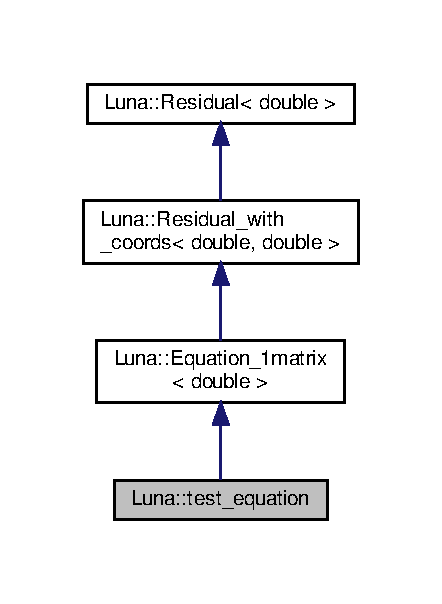
\includegraphics[width=212pt]{classLuna_1_1test__equation__inherit__graph}
\end{center}
\end{figure}


Collaboration diagram for Luna\+:\+:test\+\_\+equation\+:\nopagebreak
\begin{figure}[H]
\begin{center}
\leavevmode
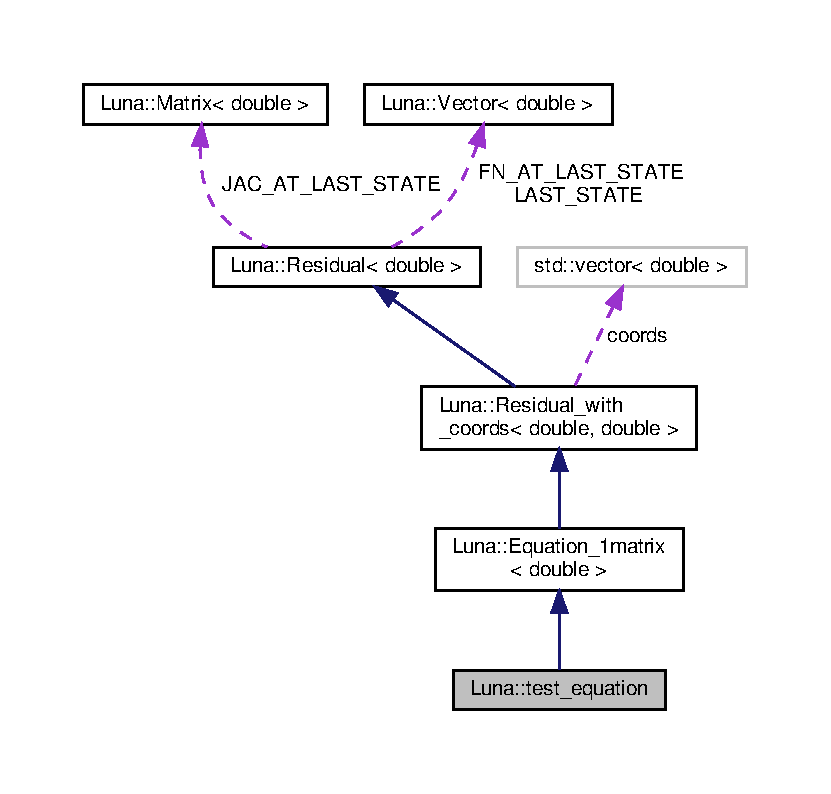
\includegraphics[width=350pt]{classLuna_1_1test__equation__coll__graph}
\end{center}
\end{figure}
\subsection*{Public Member Functions}
\begin{DoxyCompactItemize}
\item 
\hyperlink{classLuna_1_1test__equation_a76186f65e923b54c7e73faffbcefb30d}{test\+\_\+equation} ()
\item 
void \hyperlink{classLuna_1_1test__equation_a90a4576ce51729e49dbe67f36ab31f81}{residual\+\_\+fn} (const \hyperlink{classLuna_1_1Vector}{Vector}$<$ double $>$ \&u, \hyperlink{classLuna_1_1Vector}{Vector}$<$ double $>$ \&F) const
\begin{DoxyCompactList}\small\item\em The residual function to be defined later. \end{DoxyCompactList}\item 
void \hyperlink{classLuna_1_1test__equation_a955940cd7cc59fbaef213151075f1838}{matrix0} (const \hyperlink{classLuna_1_1Vector}{Vector}$<$ double $>$ \&x, \hyperlink{classLuna_1_1Matrix}{Matrix}$<$ double $>$ \&m) const
\begin{DoxyCompactList}\small\item\em Define the matrix in terms of the current state vector. \end{DoxyCompactList}\end{DoxyCompactItemize}
\subsection*{Additional Inherited Members}


\subsection{Detailed Description}


Definition at line 13 of file O\+D\+E\+\_\+\+B\+V\+P\+\_\+test.\+cpp.



\subsection{Constructor \& Destructor Documentation}
\mbox{\Hypertarget{classLuna_1_1test__equation_a76186f65e923b54c7e73faffbcefb30d}\label{classLuna_1_1test__equation_a76186f65e923b54c7e73faffbcefb30d}} 
\index{Luna\+::test\+\_\+equation@{Luna\+::test\+\_\+equation}!test\+\_\+equation@{test\+\_\+equation}}
\index{test\+\_\+equation@{test\+\_\+equation}!Luna\+::test\+\_\+equation@{Luna\+::test\+\_\+equation}}
\subsubsection{\texorpdfstring{test\+\_\+equation()}{test\_equation()}}
{\footnotesize\ttfamily Luna\+::test\+\_\+equation\+::test\+\_\+equation (\begin{DoxyParamCaption}{ }\end{DoxyParamCaption})\hspace{0.3cm}{\ttfamily [inline]}}



Definition at line 18 of file O\+D\+E\+\_\+\+B\+V\+P\+\_\+test.\+cpp.


\begin{DoxyCode}
18 : \hyperlink{classLuna_1_1Equation__1matrix}{Equation\_1matrix<double>} ( 2 ) \{\}
\end{DoxyCode}


\subsection{Member Function Documentation}
\mbox{\Hypertarget{classLuna_1_1test__equation_a955940cd7cc59fbaef213151075f1838}\label{classLuna_1_1test__equation_a955940cd7cc59fbaef213151075f1838}} 
\index{Luna\+::test\+\_\+equation@{Luna\+::test\+\_\+equation}!matrix0@{matrix0}}
\index{matrix0@{matrix0}!Luna\+::test\+\_\+equation@{Luna\+::test\+\_\+equation}}
\subsubsection{\texorpdfstring{matrix0()}{matrix0()}}
{\footnotesize\ttfamily void Luna\+::test\+\_\+equation\+::matrix0 (\begin{DoxyParamCaption}\item[{const \hyperlink{classLuna_1_1Vector}{Vector}$<$ double $>$ \&}]{x,  }\item[{\hyperlink{classLuna_1_1Matrix}{Matrix}$<$ double $>$ \&}]{m }\end{DoxyParamCaption}) const\hspace{0.3cm}{\ttfamily [inline]}, {\ttfamily [virtual]}}



Define the matrix in terms of the current state vector. 


\begin{DoxyParams}{Parameters}
{\em x} & The current state vector. \\
\hline
{\em m} & The matrix. \\
\hline
\end{DoxyParams}


Reimplemented from \hyperlink{classLuna_1_1Equation__1matrix_a2501535a6e92abc491bc491b3f64dc06}{Luna\+::\+Equation\+\_\+1matrix$<$ double $>$}.



Definition at line 28 of file O\+D\+E\+\_\+\+B\+V\+P\+\_\+test.\+cpp.



References Luna\+::\+Matrix$<$ T $>$\+::eye().


\begin{DoxyCode}
29       \{
30         m.\hyperlink{classLuna_1_1Matrix_a1b5fc5d3bfd1b03e04def5d314174be6}{eye}();
31       \}
\end{DoxyCode}
\mbox{\Hypertarget{classLuna_1_1test__equation_a90a4576ce51729e49dbe67f36ab31f81}\label{classLuna_1_1test__equation_a90a4576ce51729e49dbe67f36ab31f81}} 
\index{Luna\+::test\+\_\+equation@{Luna\+::test\+\_\+equation}!residual\+\_\+fn@{residual\+\_\+fn}}
\index{residual\+\_\+fn@{residual\+\_\+fn}!Luna\+::test\+\_\+equation@{Luna\+::test\+\_\+equation}}
\subsubsection{\texorpdfstring{residual\+\_\+fn()}{residual\_fn()}}
{\footnotesize\ttfamily void Luna\+::test\+\_\+equation\+::residual\+\_\+fn (\begin{DoxyParamCaption}\item[{const \hyperlink{classLuna_1_1Vector}{Vector}$<$ double $>$ \&}]{state,  }\item[{\hyperlink{classLuna_1_1Vector}{Vector}$<$ double $>$ \&}]{f }\end{DoxyParamCaption}) const\hspace{0.3cm}{\ttfamily [inline]}, {\ttfamily [virtual]}}



The residual function to be defined later. 


\begin{DoxyParams}{Parameters}
{\em state} & The current state \hyperlink{classLuna_1_1Vector}{Vector} \\
\hline
{\em f} & The function \hyperlink{classLuna_1_1Vector}{Vector} to be updated \\
\hline
\end{DoxyParams}


Reimplemented from \hyperlink{classLuna_1_1Residual_ae1b1ebe3314c788b176bcac7b328de5c}{Luna\+::\+Residual$<$ double $>$}.



Definition at line 21 of file O\+D\+E\+\_\+\+B\+V\+P\+\_\+test.\+cpp.



References Luna\+::\+Residual\+\_\+with\+\_\+coords$<$ double, double $>$\+::coord(), Heat\+\_\+plot\+::x, y, and yd.


\begin{DoxyCode}
22             \{
23         \textcolor{keywordtype}{double} \hyperlink{namespaceHeat__plot_aa88370c16b85b784ccbde3ed88bc1991}{x}( \hyperlink{classLuna_1_1Residual__with__coords_a3fa4c950a944743c0380e4c151728372}{coord}( 0 ) );
24                 F[ \hyperlink{ODE__BVP__test_8cpp_adf764cbdea00d65edcd07bb9953ad2b7ae1f9fdb8b786c63efc4ce44eeacd17f2}{y} ]   = \hyperlink{namespaceHeat__plot_ae622b86afa46daa3e9b887624ab1bf26}{u}[ \hyperlink{ODE__BVP__test_8cpp_adf764cbdea00d65edcd07bb9953ad2b7ae006cbf64cf3ff4ee152bf490ae2e2a7}{yd} ];
25                 F[ \hyperlink{ODE__BVP__test_8cpp_adf764cbdea00d65edcd07bb9953ad2b7ae006cbf64cf3ff4ee152bf490ae2e2a7}{yd} ]  = - 4 * \hyperlink{namespaceHeat__plot_ae622b86afa46daa3e9b887624ab1bf26}{u}[ \hyperlink{ODE__BVP__test_8cpp_adf764cbdea00d65edcd07bb9953ad2b7ae1f9fdb8b786c63efc4ce44eeacd17f2}{y} ];
26             \}
\end{DoxyCode}


The documentation for this class was generated from the following file\+:\begin{DoxyCompactItemize}
\item 
Examples/\hyperlink{ODE__BVP__test_8cpp}{O\+D\+E\+\_\+\+B\+V\+P\+\_\+test.\+cpp}\end{DoxyCompactItemize}

\hypertarget{classLuna_1_1test__residual}{}\section{Luna\+:\+:test\+\_\+residual Class Reference}
\label{classLuna_1_1test__residual}\index{Luna\+::test\+\_\+residual@{Luna\+::test\+\_\+residual}}


Inheritance diagram for Luna\+:\+:test\+\_\+residual\+:\nopagebreak
\begin{figure}[H]
\begin{center}
\leavevmode
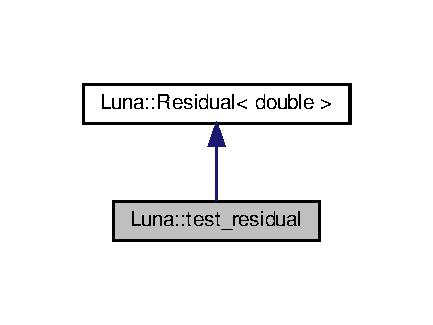
\includegraphics[width=208pt]{classLuna_1_1test__residual__inherit__graph}
\end{center}
\end{figure}


Collaboration diagram for Luna\+:\+:test\+\_\+residual\+:\nopagebreak
\begin{figure}[H]
\begin{center}
\leavevmode
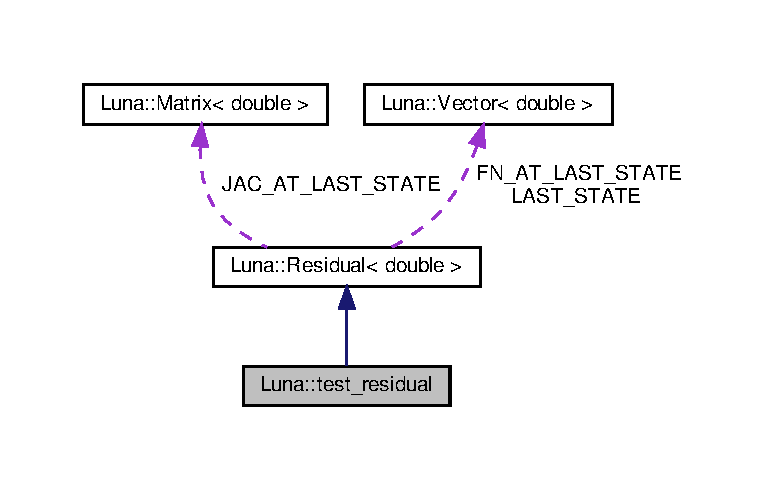
\includegraphics[width=350pt]{classLuna_1_1test__residual__coll__graph}
\end{center}
\end{figure}
\subsection*{Public Member Functions}
\begin{DoxyCompactItemize}
\item 
\hyperlink{classLuna_1_1test__residual_a5642e22c7c46d4d0e24fabb55a03e410}{test\+\_\+residual} ()
\item 
void \hyperlink{classLuna_1_1test__residual_abf5e77702d2ffec8bf2ffdc6728a8473}{residual\+\_\+fn} (const \hyperlink{classLuna_1_1Vector}{Vector}$<$ double $>$ \&x, \hyperlink{classLuna_1_1Vector}{Vector}$<$ double $>$ \&F) const
\begin{DoxyCompactList}\small\item\em The residual function to be defined later. \end{DoxyCompactList}\end{DoxyCompactItemize}
\subsection*{Additional Inherited Members}


\subsection{Detailed Description}


Definition at line 13 of file Root\+\_\+finding.\+cpp.



\subsection{Constructor \& Destructor Documentation}
\mbox{\Hypertarget{classLuna_1_1test__residual_a5642e22c7c46d4d0e24fabb55a03e410}\label{classLuna_1_1test__residual_a5642e22c7c46d4d0e24fabb55a03e410}} 
\index{Luna\+::test\+\_\+residual@{Luna\+::test\+\_\+residual}!test\+\_\+residual@{test\+\_\+residual}}
\index{test\+\_\+residual@{test\+\_\+residual}!Luna\+::test\+\_\+residual@{Luna\+::test\+\_\+residual}}
\subsubsection{\texorpdfstring{test\+\_\+residual()}{test\_residual()}}
{\footnotesize\ttfamily Luna\+::test\+\_\+residual\+::test\+\_\+residual (\begin{DoxyParamCaption}{ }\end{DoxyParamCaption})\hspace{0.3cm}{\ttfamily [inline]}}



Definition at line 17 of file Root\+\_\+finding.\+cpp.


\begin{DoxyCode}
17 : \hyperlink{classLuna_1_1Residual}{Residual<double>} ( 2 ) \{\}
\end{DoxyCode}


\subsection{Member Function Documentation}
\mbox{\Hypertarget{classLuna_1_1test__residual_abf5e77702d2ffec8bf2ffdc6728a8473}\label{classLuna_1_1test__residual_abf5e77702d2ffec8bf2ffdc6728a8473}} 
\index{Luna\+::test\+\_\+residual@{Luna\+::test\+\_\+residual}!residual\+\_\+fn@{residual\+\_\+fn}}
\index{residual\+\_\+fn@{residual\+\_\+fn}!Luna\+::test\+\_\+residual@{Luna\+::test\+\_\+residual}}
\subsubsection{\texorpdfstring{residual\+\_\+fn()}{residual\_fn()}}
{\footnotesize\ttfamily void Luna\+::test\+\_\+residual\+::residual\+\_\+fn (\begin{DoxyParamCaption}\item[{const \hyperlink{classLuna_1_1Vector}{Vector}$<$ double $>$ \&}]{state,  }\item[{\hyperlink{classLuna_1_1Vector}{Vector}$<$ double $>$ \&}]{f }\end{DoxyParamCaption}) const\hspace{0.3cm}{\ttfamily [inline]}, {\ttfamily [virtual]}}



The residual function to be defined later. 


\begin{DoxyParams}{Parameters}
{\em state} & The current state \hyperlink{classLuna_1_1Vector}{Vector} \\
\hline
{\em f} & The function \hyperlink{classLuna_1_1Vector}{Vector} to be updated \\
\hline
\end{DoxyParams}


Reimplemented from \hyperlink{classLuna_1_1Residual_ae1b1ebe3314c788b176bcac7b328de5c}{Luna\+::\+Residual$<$ double $>$}.



Definition at line 20 of file Root\+\_\+finding.\+cpp.


\begin{DoxyCode}
21             \{
22                 F[ 0 ] = std::pow( \hyperlink{namespaceHeat__plot_aa88370c16b85b784ccbde3ed88bc1991}{x}[ 0 ], 3.0 ) + \hyperlink{namespaceHeat__plot_aa88370c16b85b784ccbde3ed88bc1991}{x}[ 1 ] - 1;
23                 F[ 1 ] = std::pow( \hyperlink{namespaceHeat__plot_aa88370c16b85b784ccbde3ed88bc1991}{x}[ 1 ], 3.0 ) - \hyperlink{namespaceHeat__plot_aa88370c16b85b784ccbde3ed88bc1991}{x}[ 0 ] + 1;
24                 \textcolor{comment}{/*}
25 \textcolor{comment}{                    x^3 + y - 1 = 0,}
26 \textcolor{comment}{                    y^3 - x + 1 = 0,}
27 \textcolor{comment}{                    (x,y) = (1,0) is the only (real) solution}
28 \textcolor{comment}{                */}
29             \}
\end{DoxyCode}


The documentation for this class was generated from the following file\+:\begin{DoxyCompactItemize}
\item 
Examples/\hyperlink{Root__finding_8cpp}{Root\+\_\+finding.\+cpp}\end{DoxyCompactItemize}

\hypertarget{classLuna_1_1Timer}{}\section{Luna\+:\+:Timer Class Reference}
\label{classLuna_1_1Timer}\index{Luna\+::\+Timer@{Luna\+::\+Timer}}


A simple timer class for timing methods.  




{\ttfamily \#include $<$Timer.\+h$>$}

\subsection*{Public Member Functions}
\begin{DoxyCompactItemize}
\item 
\hyperlink{classLuna_1_1Timer_a8505121ba140f41121a57e4404e1d251}{Timer} ()
\begin{DoxyCompactList}\small\item\em Constructor. \end{DoxyCompactList}\item 
\hyperlink{classLuna_1_1Timer_af53efaf19a32dd49cc3c84671603d352}{$\sim$\+Timer} ()
\begin{DoxyCompactList}\small\item\em Destructor. \end{DoxyCompactList}\item 
bool \hyperlink{classLuna_1_1Timer_acd735003d27555b69bc3c54e8cd4a301}{is\+\_\+started} ()
\begin{DoxyCompactList}\small\item\em Check if the timer has started. \end{DoxyCompactList}\item 
bool \hyperlink{classLuna_1_1Timer_aa028fb717dce42cbf9806ce604ba09b6}{is\+\_\+stopped} ()
\begin{DoxyCompactList}\small\item\em Check if the timer is stopped. \end{DoxyCompactList}\item 
bool \hyperlink{classLuna_1_1Timer_a006199b985e14e421d7dc1ef5d6e08a8}{is\+\_\+paused} ()
\begin{DoxyCompactList}\small\item\em Check if the timer is paused. \end{DoxyCompactList}\item 
bool \hyperlink{classLuna_1_1Timer_a025d787c4a3c7cc94e920e0ae480488f}{is\+\_\+active} ()
\begin{DoxyCompactList}\small\item\em Check if the timer is active. \end{DoxyCompactList}\item 
void \hyperlink{classLuna_1_1Timer_af2663caeb132da9375669733ac826cc8}{pause} ()
\begin{DoxyCompactList}\small\item\em Pause the timer. \end{DoxyCompactList}\item 
void \hyperlink{classLuna_1_1Timer_abf0e92e9d430cdf42c0ebe21e8220c91}{resume} ()
\begin{DoxyCompactList}\small\item\em Resume the timer. \end{DoxyCompactList}\item 
void \hyperlink{classLuna_1_1Timer_ab074740a502b02be0bb64ef3320733b3}{start} ()
\begin{DoxyCompactList}\small\item\em Start the timer. \end{DoxyCompactList}\item 
void \hyperlink{classLuna_1_1Timer_ad8ba9deb09bfe422cfaadba04a776662}{stop} ()
\begin{DoxyCompactList}\small\item\em Stop the timer. \end{DoxyCompactList}\item 
void \hyperlink{classLuna_1_1Timer_a7aee89c76f083206cb1ce7fd150f4e81}{reset} ()
\begin{DoxyCompactList}\small\item\em Reset the timer. \end{DoxyCompactList}\item 
void \hyperlink{classLuna_1_1Timer_ac0292bd7a6e45b269919fc2fe160a8bf}{print} () const
\begin{DoxyCompactList}\small\item\em Output the time to the screen. \end{DoxyCompactList}\item 
double \hyperlink{classLuna_1_1Timer_ac8b59a9f3d149ec56156af6f74a6d1a9}{get\+\_\+time} () const
\begin{DoxyCompactList}\small\item\em Return the time in milliseconds. \end{DoxyCompactList}\item 
clock\+\_\+t \hyperlink{classLuna_1_1Timer_a7b9ca4a1299e21bb5690aa960612ae9e}{get\+\_\+ticks} ()
\begin{DoxyCompactList}\small\item\em Return the number of clock ticks. \end{DoxyCompactList}\end{DoxyCompactItemize}


\subsection{Detailed Description}
A simple timer class for timing methods. 

Definition at line 13 of file Timer.\+h.



\subsection{Constructor \& Destructor Documentation}
\mbox{\Hypertarget{classLuna_1_1Timer_a8505121ba140f41121a57e4404e1d251}\label{classLuna_1_1Timer_a8505121ba140f41121a57e4404e1d251}} 
\index{Luna\+::\+Timer@{Luna\+::\+Timer}!Timer@{Timer}}
\index{Timer@{Timer}!Luna\+::\+Timer@{Luna\+::\+Timer}}
\subsubsection{\texorpdfstring{Timer()}{Timer()}}
{\footnotesize\ttfamily Luna\+::\+Timer\+::\+Timer (\begin{DoxyParamCaption}{ }\end{DoxyParamCaption})\hspace{0.3cm}{\ttfamily [inline]}}



Constructor. 



Definition at line 27 of file Timer.\+h.


\begin{DoxyCode}
27                 : START\_TIME( 0 ), PAUSED\_TIME( 0 ), STARTED( \textcolor{keyword}{false} ), PAUSED( \textcolor{keyword}{false} )
28         \{\}
\end{DoxyCode}
\mbox{\Hypertarget{classLuna_1_1Timer_af53efaf19a32dd49cc3c84671603d352}\label{classLuna_1_1Timer_af53efaf19a32dd49cc3c84671603d352}} 
\index{Luna\+::\+Timer@{Luna\+::\+Timer}!````~Timer@{$\sim$\+Timer}}
\index{````~Timer@{$\sim$\+Timer}!Luna\+::\+Timer@{Luna\+::\+Timer}}
\subsubsection{\texorpdfstring{$\sim$\+Timer()}{~Timer()}}
{\footnotesize\ttfamily Luna\+::\+Timer\+::$\sim$\+Timer (\begin{DoxyParamCaption}{ }\end{DoxyParamCaption})\hspace{0.3cm}{\ttfamily [inline]}}



Destructor. 



Definition at line 31 of file Timer.\+h.



References get\+\_\+ticks(), get\+\_\+time(), is\+\_\+active(), is\+\_\+paused(), is\+\_\+started(), is\+\_\+stopped(), pause(), print(), reset(), resume(), start(), and stop().


\begin{DoxyCode}
32         \{\}
\end{DoxyCode}


\subsection{Member Function Documentation}
\mbox{\Hypertarget{classLuna_1_1Timer_a7b9ca4a1299e21bb5690aa960612ae9e}\label{classLuna_1_1Timer_a7b9ca4a1299e21bb5690aa960612ae9e}} 
\index{Luna\+::\+Timer@{Luna\+::\+Timer}!get\+\_\+ticks@{get\+\_\+ticks}}
\index{get\+\_\+ticks@{get\+\_\+ticks}!Luna\+::\+Timer@{Luna\+::\+Timer}}
\subsubsection{\texorpdfstring{get\+\_\+ticks()}{get\_ticks()}}
{\footnotesize\ttfamily clock\+\_\+t Luna\+::\+Timer\+::get\+\_\+ticks (\begin{DoxyParamCaption}{ }\end{DoxyParamCaption})\hspace{0.3cm}{\ttfamily [inline]}}



Return the number of clock ticks. 

\begin{DoxyReturn}{Returns}
The number of clock ticks 
\end{DoxyReturn}


Definition at line 165 of file Timer.\+h.



Referenced by get\+\_\+time(), and $\sim$\+Timer().


\begin{DoxyCode}
166     \{
167         \textcolor{keywordflow}{if}( !STARTED )
168         \{
169             \textcolor{keywordflow}{return} 0;
170         \}
171 
172         \textcolor{keywordflow}{if}( PAUSED )
173         \{
174             \textcolor{keywordflow}{return} PAUSED\_TIME - START\_TIME;
175         \}
176 
177         \textcolor{keywordflow}{return} clock() - START\_TIME;
178     \}
\end{DoxyCode}
\mbox{\Hypertarget{classLuna_1_1Timer_ac8b59a9f3d149ec56156af6f74a6d1a9}\label{classLuna_1_1Timer_ac8b59a9f3d149ec56156af6f74a6d1a9}} 
\index{Luna\+::\+Timer@{Luna\+::\+Timer}!get\+\_\+time@{get\+\_\+time}}
\index{get\+\_\+time@{get\+\_\+time}!Luna\+::\+Timer@{Luna\+::\+Timer}}
\subsubsection{\texorpdfstring{get\+\_\+time()}{get\_time()}}
{\footnotesize\ttfamily double Luna\+::\+Timer\+::get\+\_\+time (\begin{DoxyParamCaption}{ }\end{DoxyParamCaption}) const\hspace{0.3cm}{\ttfamily [inline]}}



Return the time in milliseconds. 

\begin{DoxyReturn}{Returns}
The time in ms 
\end{DoxyReturn}


Definition at line 159 of file Timer.\+h.



References get\+\_\+ticks().



Referenced by main(), print(), and $\sim$\+Timer().


\begin{DoxyCode}
160     \{
161         \hyperlink{classLuna_1_1Timer_a8505121ba140f41121a57e4404e1d251}{Timer} temp( *\textcolor{keyword}{this} );
162         \textcolor{keywordflow}{return} 1.e3 * temp.get\_ticks() / CLOCKS\_PER\_SEC;
163     \}
\end{DoxyCode}
\mbox{\Hypertarget{classLuna_1_1Timer_a025d787c4a3c7cc94e920e0ae480488f}\label{classLuna_1_1Timer_a025d787c4a3c7cc94e920e0ae480488f}} 
\index{Luna\+::\+Timer@{Luna\+::\+Timer}!is\+\_\+active@{is\+\_\+active}}
\index{is\+\_\+active@{is\+\_\+active}!Luna\+::\+Timer@{Luna\+::\+Timer}}
\subsubsection{\texorpdfstring{is\+\_\+active()}{is\_active()}}
{\footnotesize\ttfamily bool Luna\+::\+Timer\+::is\+\_\+active (\begin{DoxyParamCaption}{ }\end{DoxyParamCaption})\hspace{0.3cm}{\ttfamily [inline]}}



Check if the timer is active. 

\begin{DoxyReturn}{Returns}
true if the timer is still active and false otherwise 
\end{DoxyReturn}


Definition at line 97 of file Timer.\+h.



Referenced by $\sim$\+Timer().


\begin{DoxyCode}
98     \{
99         \textcolor{keywordflow}{return} !PAUSED & STARTED;
100     \}
\end{DoxyCode}
\mbox{\Hypertarget{classLuna_1_1Timer_a006199b985e14e421d7dc1ef5d6e08a8}\label{classLuna_1_1Timer_a006199b985e14e421d7dc1ef5d6e08a8}} 
\index{Luna\+::\+Timer@{Luna\+::\+Timer}!is\+\_\+paused@{is\+\_\+paused}}
\index{is\+\_\+paused@{is\+\_\+paused}!Luna\+::\+Timer@{Luna\+::\+Timer}}
\subsubsection{\texorpdfstring{is\+\_\+paused()}{is\_paused()}}
{\footnotesize\ttfamily bool Luna\+::\+Timer\+::is\+\_\+paused (\begin{DoxyParamCaption}{ }\end{DoxyParamCaption})\hspace{0.3cm}{\ttfamily [inline]}}



Check if the timer is paused. 

\begin{DoxyReturn}{Returns}
true if the timer is paused and false otherwise 
\end{DoxyReturn}


Definition at line 92 of file Timer.\+h.



Referenced by $\sim$\+Timer().


\begin{DoxyCode}
93     \{
94         \textcolor{keywordflow}{return} PAUSED;
95     \}
\end{DoxyCode}
\mbox{\Hypertarget{classLuna_1_1Timer_acd735003d27555b69bc3c54e8cd4a301}\label{classLuna_1_1Timer_acd735003d27555b69bc3c54e8cd4a301}} 
\index{Luna\+::\+Timer@{Luna\+::\+Timer}!is\+\_\+started@{is\+\_\+started}}
\index{is\+\_\+started@{is\+\_\+started}!Luna\+::\+Timer@{Luna\+::\+Timer}}
\subsubsection{\texorpdfstring{is\+\_\+started()}{is\_started()}}
{\footnotesize\ttfamily bool Luna\+::\+Timer\+::is\+\_\+started (\begin{DoxyParamCaption}{ }\end{DoxyParamCaption})\hspace{0.3cm}{\ttfamily [inline]}}



Check if the timer has started. 

\begin{DoxyReturn}{Returns}
true if the time has been started and false otherwise 
\end{DoxyReturn}


Definition at line 82 of file Timer.\+h.



Referenced by $\sim$\+Timer().


\begin{DoxyCode}
83     \{
84         \textcolor{keywordflow}{return} STARTED;
85     \}
\end{DoxyCode}
\mbox{\Hypertarget{classLuna_1_1Timer_aa028fb717dce42cbf9806ce604ba09b6}\label{classLuna_1_1Timer_aa028fb717dce42cbf9806ce604ba09b6}} 
\index{Luna\+::\+Timer@{Luna\+::\+Timer}!is\+\_\+stopped@{is\+\_\+stopped}}
\index{is\+\_\+stopped@{is\+\_\+stopped}!Luna\+::\+Timer@{Luna\+::\+Timer}}
\subsubsection{\texorpdfstring{is\+\_\+stopped()}{is\_stopped()}}
{\footnotesize\ttfamily bool Luna\+::\+Timer\+::is\+\_\+stopped (\begin{DoxyParamCaption}{ }\end{DoxyParamCaption})\hspace{0.3cm}{\ttfamily [inline]}}



Check if the timer is stopped. 

\begin{DoxyReturn}{Returns}
true if the timer is stopped and false otherwise 
\end{DoxyReturn}


Definition at line 87 of file Timer.\+h.



Referenced by $\sim$\+Timer().


\begin{DoxyCode}
88     \{
89         \textcolor{keywordflow}{return} !STARTED;
90     \}
\end{DoxyCode}
\mbox{\Hypertarget{classLuna_1_1Timer_af2663caeb132da9375669733ac826cc8}\label{classLuna_1_1Timer_af2663caeb132da9375669733ac826cc8}} 
\index{Luna\+::\+Timer@{Luna\+::\+Timer}!pause@{pause}}
\index{pause@{pause}!Luna\+::\+Timer@{Luna\+::\+Timer}}
\subsubsection{\texorpdfstring{pause()}{pause()}}
{\footnotesize\ttfamily void Luna\+::\+Timer\+::pause (\begin{DoxyParamCaption}{ }\end{DoxyParamCaption})\hspace{0.3cm}{\ttfamily [inline]}}



Pause the timer. 



Definition at line 102 of file Timer.\+h.



Referenced by $\sim$\+Timer().


\begin{DoxyCode}
103     \{
104         \textcolor{keywordflow}{if}( PAUSED || !STARTED )
105         \{
106             \textcolor{keywordflow}{return};
107         \}
108         PAUSED = \textcolor{keyword}{true};
109         PAUSED\_TIME = clock();
110     \}
\end{DoxyCode}
\mbox{\Hypertarget{classLuna_1_1Timer_ac0292bd7a6e45b269919fc2fe160a8bf}\label{classLuna_1_1Timer_ac0292bd7a6e45b269919fc2fe160a8bf}} 
\index{Luna\+::\+Timer@{Luna\+::\+Timer}!print@{print}}
\index{print@{print}!Luna\+::\+Timer@{Luna\+::\+Timer}}
\subsubsection{\texorpdfstring{print()}{print()}}
{\footnotesize\ttfamily void Luna\+::\+Timer\+::print (\begin{DoxyParamCaption}{ }\end{DoxyParamCaption}) const\hspace{0.3cm}{\ttfamily [inline]}}



Output the time to the screen. 



Definition at line 144 of file Timer.\+h.



References get\+\_\+time().



Referenced by main(), and $\sim$\+Timer().


\begin{DoxyCode}
145     \{
146         std::cout.precision(4);
147         \hyperlink{classLuna_1_1Timer_a8505121ba140f41121a57e4404e1d251}{Timer} temp( *\textcolor{keyword}{this} );
148         \textcolor{keyword}{const} \textcolor{keywordtype}{double} elapsed\_time\_in\_ms( temp.get\_time() );
149         \textcolor{keywordflow}{if} ( elapsed\_time\_in\_ms > 1000 )
150         \{
151           std::cout << \textcolor{stringliteral}{"  * TOTAL CPU time taken = "} << elapsed\_time\_in\_ms / 1000. << \textcolor{stringliteral}{" s\(\backslash\)n"};
152         \}
153         \textcolor{keywordflow}{else}
154         \{
155          std::cout << \textcolor{stringliteral}{"  * TOTAL CPU time taken = "} << elapsed\_time\_in\_ms << \textcolor{stringliteral}{" ms\(\backslash\)n"};
156         \}
157     \}
\end{DoxyCode}
\mbox{\Hypertarget{classLuna_1_1Timer_a7aee89c76f083206cb1ce7fd150f4e81}\label{classLuna_1_1Timer_a7aee89c76f083206cb1ce7fd150f4e81}} 
\index{Luna\+::\+Timer@{Luna\+::\+Timer}!reset@{reset}}
\index{reset@{reset}!Luna\+::\+Timer@{Luna\+::\+Timer}}
\subsubsection{\texorpdfstring{reset()}{reset()}}
{\footnotesize\ttfamily void Luna\+::\+Timer\+::reset (\begin{DoxyParamCaption}{ }\end{DoxyParamCaption})\hspace{0.3cm}{\ttfamily [inline]}}



Reset the timer. 



Definition at line 138 of file Timer.\+h.



Referenced by $\sim$\+Timer().


\begin{DoxyCode}
139     \{
140         PAUSED = \textcolor{keyword}{false};
141         START\_TIME = clock();
142     \}
\end{DoxyCode}
\mbox{\Hypertarget{classLuna_1_1Timer_abf0e92e9d430cdf42c0ebe21e8220c91}\label{classLuna_1_1Timer_abf0e92e9d430cdf42c0ebe21e8220c91}} 
\index{Luna\+::\+Timer@{Luna\+::\+Timer}!resume@{resume}}
\index{resume@{resume}!Luna\+::\+Timer@{Luna\+::\+Timer}}
\subsubsection{\texorpdfstring{resume()}{resume()}}
{\footnotesize\ttfamily void Luna\+::\+Timer\+::resume (\begin{DoxyParamCaption}{ }\end{DoxyParamCaption})\hspace{0.3cm}{\ttfamily [inline]}}



Resume the timer. 



Definition at line 112 of file Timer.\+h.



Referenced by $\sim$\+Timer().


\begin{DoxyCode}
113     \{
114         \textcolor{keywordflow}{if}( !PAUSED )
115         \{
116             \textcolor{keywordflow}{return};
117         \}
118         PAUSED = \textcolor{keyword}{false};
119         START\_TIME += clock() - PAUSED\_TIME;
120     \}
\end{DoxyCode}
\mbox{\Hypertarget{classLuna_1_1Timer_ab074740a502b02be0bb64ef3320733b3}\label{classLuna_1_1Timer_ab074740a502b02be0bb64ef3320733b3}} 
\index{Luna\+::\+Timer@{Luna\+::\+Timer}!start@{start}}
\index{start@{start}!Luna\+::\+Timer@{Luna\+::\+Timer}}
\subsubsection{\texorpdfstring{start()}{start()}}
{\footnotesize\ttfamily void Luna\+::\+Timer\+::start (\begin{DoxyParamCaption}{ }\end{DoxyParamCaption})\hspace{0.3cm}{\ttfamily [inline]}}



Start the timer. 



Definition at line 122 of file Timer.\+h.



Referenced by main(), and $\sim$\+Timer().


\begin{DoxyCode}
123     \{
124         \textcolor{keywordflow}{if}( STARTED )
125         \{
126             \textcolor{keywordflow}{return};
127         \}
128         STARTED = \textcolor{keyword}{true};
129         PAUSED = \textcolor{keyword}{false};
130         START\_TIME = clock();
131     \}
\end{DoxyCode}
\mbox{\Hypertarget{classLuna_1_1Timer_ad8ba9deb09bfe422cfaadba04a776662}\label{classLuna_1_1Timer_ad8ba9deb09bfe422cfaadba04a776662}} 
\index{Luna\+::\+Timer@{Luna\+::\+Timer}!stop@{stop}}
\index{stop@{stop}!Luna\+::\+Timer@{Luna\+::\+Timer}}
\subsubsection{\texorpdfstring{stop()}{stop()}}
{\footnotesize\ttfamily void Luna\+::\+Timer\+::stop (\begin{DoxyParamCaption}{ }\end{DoxyParamCaption})\hspace{0.3cm}{\ttfamily [inline]}}



Stop the timer. 



Definition at line 133 of file Timer.\+h.



Referenced by main(), and $\sim$\+Timer().


\begin{DoxyCode}
134     \{
135         STARTED = \textcolor{keyword}{false};
136     \}
\end{DoxyCode}


The documentation for this class was generated from the following file\+:\begin{DoxyCompactItemize}
\item 
include/\+Luna/\hyperlink{Timer_8h}{Timer.\+h}\end{DoxyCompactItemize}

\hypertarget{classLuna_1_1Tridiagonal}{}\section{Luna\+:\+:Tridiagonal$<$ T $>$ Class Template Reference}
\label{classLuna_1_1Tridiagonal}\index{Luna\+::\+Tridiagonal$<$ T $>$@{Luna\+::\+Tridiagonal$<$ T $>$}}


A \hyperlink{classLuna_1_1Tridiagonal}{Tridiagonal} matrix class for use with double and std\+::complex$<$double$>$  




{\ttfamily \#include $<$Tridiagonal.\+h$>$}

\subsection*{Public Member Functions}
\begin{DoxyCompactItemize}
\item 
\hyperlink{classLuna_1_1Tridiagonal_a749d1915ad40623c14046c690c6f16af}{Tridiagonal} ()
\begin{DoxyCompactList}\small\item\em Constructor for an empty \hyperlink{classLuna_1_1Tridiagonal}{Tridiagonal} matrix of unspecified size. \end{DoxyCompactList}\item 
\hyperlink{classLuna_1_1Tridiagonal_a34075ccfbb407b9f29e9f867813d1958}{Tridiagonal} (const std\+::size\+\_\+t \&\hyperlink{classLuna_1_1Tridiagonal_ae8586e82968a8c28f7c50008e1f75411}{size})
\begin{DoxyCompactList}\small\item\em Constructor for a \hyperlink{classLuna_1_1Tridiagonal}{Tridiagonal} matrix of specified size. \end{DoxyCompactList}\item 
\hyperlink{classLuna_1_1Tridiagonal_ab723eb17bd32e82fb6e27e2170b4cccc}{Tridiagonal} (const \hyperlink{classLuna_1_1Vector}{Vector}$<$ T $>$ \&sub, const \hyperlink{classLuna_1_1Vector}{Vector}$<$ T $>$ \&\hyperlink{Vector__algebra_8cpp_ae66f6b31b5ad750f1fe042a706a4e3d4}{main}, const \hyperlink{classLuna_1_1Vector}{Vector}$<$ T $>$ \&super)
\begin{DoxyCompactList}\small\item\em Constructor for a \hyperlink{classLuna_1_1Tridiagonal}{Tridiagonal} matrix using specified Vectors. \end{DoxyCompactList}\item 
\hyperlink{classLuna_1_1Tridiagonal_a43f06132888b27c66355ac7971089947}{Tridiagonal} (const T \&sub\+\_\+elem, const T \&main\+\_\+elem, const T \&super\+\_\+elem, const std\+::size\+\_\+t n)
\begin{DoxyCompactList}\small\item\em Constructor for a \hyperlink{classLuna_1_1Tridiagonal}{Tridiagonal} matrix using specified elements. \end{DoxyCompactList}\item 
\hyperlink{classLuna_1_1Tridiagonal_a9051546ef7a37559b1edff2a48d9741c}{$\sim$\+Tridiagonal} ()
\begin{DoxyCompactList}\small\item\em Destructor. \end{DoxyCompactList}\item 
const T \& \hyperlink{classLuna_1_1Tridiagonal_aa94d8c34b275eb5f6de7a840b78b843f}{operator()} (const std\+::size\+\_\+t \&i, const std\+::size\+\_\+t \&j) const
\begin{DoxyCompactList}\small\item\em Indexing operator ( read only ) \end{DoxyCompactList}\item 
T \& \hyperlink{classLuna_1_1Tridiagonal_ae5bbfe810d68ead053a4178d742c58ea}{operator()} (const std\+::size\+\_\+t \&i, const std\+::size\+\_\+t \&j)
\begin{DoxyCompactList}\small\item\em Indexing operator ( read / write ) \end{DoxyCompactList}\item 
\hyperlink{classLuna_1_1Tridiagonal}{Tridiagonal}$<$ T $>$ \& \hyperlink{classLuna_1_1Tridiagonal_a0118c1de81c85bd371d166390a4e5d4b}{operator=} (const \hyperlink{classLuna_1_1Tridiagonal}{Tridiagonal}$<$ T $>$ \&original)
\begin{DoxyCompactList}\small\item\em Copy assignment. \end{DoxyCompactList}\item 
\hyperlink{classLuna_1_1Tridiagonal}{Tridiagonal}$<$ T $>$ \hyperlink{classLuna_1_1Tridiagonal_a654145a044a7fda0de429ece11915781}{operator+} () const
\begin{DoxyCompactList}\small\item\em Unary +. \end{DoxyCompactList}\item 
\hyperlink{classLuna_1_1Tridiagonal}{Tridiagonal}$<$ T $>$ \hyperlink{classLuna_1_1Tridiagonal_a7f92f3637e30a2fcc12fa959e00eefa0}{operator-\/} () const
\begin{DoxyCompactList}\small\item\em Unary -\/. \end{DoxyCompactList}\item 
\hyperlink{classLuna_1_1Tridiagonal}{Tridiagonal}$<$ T $>$ \hyperlink{classLuna_1_1Tridiagonal_a8e28947c6514a84755620ee96400c9cb}{operator+} (const \hyperlink{classLuna_1_1Tridiagonal}{Tridiagonal}$<$ T $>$ \&m\+\_\+plus) const
\begin{DoxyCompactList}\small\item\em Binary +. \end{DoxyCompactList}\item 
\hyperlink{classLuna_1_1Tridiagonal}{Tridiagonal}$<$ T $>$ \hyperlink{classLuna_1_1Tridiagonal_ada353bc1778051728e37403d71f57a34}{operator-\/} (const \hyperlink{classLuna_1_1Tridiagonal}{Tridiagonal}$<$ T $>$ \&m\+\_\+minus) const
\begin{DoxyCompactList}\small\item\em Binary -\/. \end{DoxyCompactList}\item 
\hyperlink{classLuna_1_1Tridiagonal}{Tridiagonal}$<$ T $>$ \hyperlink{classLuna_1_1Tridiagonal_a5dfe657389e0cb8af507ea77a8fda4e1}{operator$\ast$} (const T \&scalar) const
\begin{DoxyCompactList}\small\item\em Scalar multiplication. \end{DoxyCompactList}\item 
\hyperlink{classLuna_1_1Tridiagonal}{Tridiagonal}$<$ T $>$ \hyperlink{classLuna_1_1Tridiagonal_a3994e79c15f9848a1c1badb19247c1c7}{operator/} (const T \&divisor) const
\begin{DoxyCompactList}\small\item\em Scalar division. \end{DoxyCompactList}\item 
\hyperlink{classLuna_1_1Tridiagonal}{Tridiagonal}$<$ T $>$ \& \hyperlink{classLuna_1_1Tridiagonal_a5f34fd29d4ba9f517897a4c9eafa8157}{operator+=} (const \hyperlink{classLuna_1_1Tridiagonal}{Tridiagonal}$<$ T $>$ \&m\+\_\+plus)
\begin{DoxyCompactList}\small\item\em Addition assignment. \end{DoxyCompactList}\item 
\hyperlink{classLuna_1_1Tridiagonal}{Tridiagonal}$<$ T $>$ \& \hyperlink{classLuna_1_1Tridiagonal_ae4371d0bd7267737984ab697968f9eac}{operator-\/=} (const \hyperlink{classLuna_1_1Tridiagonal}{Tridiagonal}$<$ T $>$ \&m\+\_\+minus)
\begin{DoxyCompactList}\small\item\em Subtraction assignment. \end{DoxyCompactList}\item 
\hyperlink{classLuna_1_1Tridiagonal}{Tridiagonal}$<$ T $>$ \& \hyperlink{classLuna_1_1Tridiagonal_ad2050805abc012920f7c29cbf93989c3}{operator$\ast$=} (const T \&scalar)
\begin{DoxyCompactList}\small\item\em Scalar multiplication assignment. \end{DoxyCompactList}\item 
\hyperlink{classLuna_1_1Tridiagonal}{Tridiagonal}$<$ T $>$ \& \hyperlink{classLuna_1_1Tridiagonal_a0508de0c1797db737adaff1a6ee63763}{operator/=} (const T \&divisor)
\begin{DoxyCompactList}\small\item\em Scalar division assigment. \end{DoxyCompactList}\item 
\hyperlink{classLuna_1_1Tridiagonal}{Tridiagonal}$<$ T $>$ \& \hyperlink{classLuna_1_1Tridiagonal_aed6025d2b9420b4eb7488c2a644c1110}{operator+=} (const T \&add)
\begin{DoxyCompactList}\small\item\em Constant addition assignment. \end{DoxyCompactList}\item 
\hyperlink{classLuna_1_1Tridiagonal}{Tridiagonal}$<$ T $>$ \& \hyperlink{classLuna_1_1Tridiagonal_a77da1de7d41e6da4e7b99dc5e571a3a3}{operator-\/=} (const T \&minus)
\begin{DoxyCompactList}\small\item\em Constant subtraction assignment. \end{DoxyCompactList}\item 
\hyperlink{classLuna_1_1Vector}{Vector}$<$ T $>$ \hyperlink{classLuna_1_1Tridiagonal_a5262edb6caa8aac0186c480c3be2dcf2}{operator$\ast$} (\hyperlink{classLuna_1_1Vector}{Vector}$<$ T $>$ \&x)
\begin{DoxyCompactList}\small\item\em \hyperlink{classLuna_1_1Tridiagonal}{Tridiagonal} matrix \hyperlink{classLuna_1_1Vector}{Vector} multiplication. \end{DoxyCompactList}\item 
std\+::size\+\_\+t \hyperlink{classLuna_1_1Tridiagonal_ae8586e82968a8c28f7c50008e1f75411}{size} () const
\begin{DoxyCompactList}\small\item\em Size of the main diagonal of the matrix. \end{DoxyCompactList}\item 
void \hyperlink{classLuna_1_1Tridiagonal_a6d131d4c600e591c49e7825b52a1021c}{set\+\_\+sub} (const \hyperlink{classLuna_1_1Vector}{Vector}$<$ T $>$ \&sub)
\begin{DoxyCompactList}\small\item\em Set the subdiagonal of the matrix. \end{DoxyCompactList}\item 
void \hyperlink{classLuna_1_1Tridiagonal_a6594e3223659a5e9c7b911cda11ec5b3}{set\+\_\+main} (const \hyperlink{classLuna_1_1Vector}{Vector}$<$ T $>$ \&\hyperlink{Vector__algebra_8cpp_ae66f6b31b5ad750f1fe042a706a4e3d4}{main})
\begin{DoxyCompactList}\small\item\em Set the main diagonal of the matrix. \end{DoxyCompactList}\item 
void \hyperlink{classLuna_1_1Tridiagonal_a875d22427ef3a88accb530fe9806bfa4}{set\+\_\+super} (const \hyperlink{classLuna_1_1Vector}{Vector}$<$ T $>$ \&super)
\begin{DoxyCompactList}\small\item\em Set the superdiagonal of the matrix. \end{DoxyCompactList}\item 
void \hyperlink{classLuna_1_1Tridiagonal_a288b97194054318128a096aac12a7eef}{set\+\_\+sub} (const T \&sub\+\_\+elem)
\begin{DoxyCompactList}\small\item\em Set the subdiagonal of the matrix. \end{DoxyCompactList}\item 
void \hyperlink{classLuna_1_1Tridiagonal_a2c333c2bd6de2d9432a2325979240c93}{set\+\_\+main} (const T \&main\+\_\+elem)
\begin{DoxyCompactList}\small\item\em Set the main diagonal of the matrix. \end{DoxyCompactList}\item 
void \hyperlink{classLuna_1_1Tridiagonal_a956689dcbe76a4b23fa10192a7e1a8f9}{set\+\_\+super} (const T \&super\+\_\+elem)
\begin{DoxyCompactList}\small\item\em Set the superdiagonal of the matrix. \end{DoxyCompactList}\item 
\hyperlink{classLuna_1_1Vector}{Vector}$<$ T $>$ \hyperlink{classLuna_1_1Tridiagonal_a00675dffdb07936a5252d2a32ca3d983}{get\+\_\+sub} ()
\begin{DoxyCompactList}\small\item\em Get the subdiagonal of the matrix. \end{DoxyCompactList}\item 
\hyperlink{classLuna_1_1Vector}{Vector}$<$ T $>$ \hyperlink{classLuna_1_1Tridiagonal_ac95e35aacc68963b5889f0cf6c838315}{get\+\_\+main} ()
\begin{DoxyCompactList}\small\item\em Get the main diagonal of the matrix. \end{DoxyCompactList}\item 
\hyperlink{classLuna_1_1Vector}{Vector}$<$ T $>$ \hyperlink{classLuna_1_1Tridiagonal_aeb826920a890dec25c7817418ccaa8cb}{get\+\_\+super} ()
\begin{DoxyCompactList}\small\item\em Get the superdiagonal of the matrix. \end{DoxyCompactList}\item 
\hyperlink{classLuna_1_1Vector}{Vector}$<$ T $>$ \hyperlink{classLuna_1_1Tridiagonal_a4199f825838490b1a708dfa953963ce5}{get\+\_\+row} (const std\+::size\+\_\+t \&row)
\begin{DoxyCompactList}\small\item\em Get a row of the tridiagonal matrix as a \hyperlink{classLuna_1_1Vector}{Vector}. \end{DoxyCompactList}\item 
void \hyperlink{classLuna_1_1Tridiagonal_a97a6ebf42711983a047675211e2a277b}{transpose\+\_\+in\+\_\+place} ()
\begin{DoxyCompactList}\small\item\em Replace the current \hyperlink{classLuna_1_1Matrix}{Matrix} with its transpose. \end{DoxyCompactList}\item 
\hyperlink{classLuna_1_1Tridiagonal}{Tridiagonal}$<$ T $>$ \hyperlink{classLuna_1_1Tridiagonal_ad4a4209b7a20a65fce5c66444af3249e}{transpose} () const
\begin{DoxyCompactList}\small\item\em Return the transpose of the \hyperlink{classLuna_1_1Matrix}{Matrix}. \end{DoxyCompactList}\item 
void \hyperlink{classLuna_1_1Tridiagonal_aafeede93e34d8418725ae97c645e54cc}{resize} (const std\+::size\+\_\+t \&\hyperlink{classLuna_1_1Tridiagonal_ae8586e82968a8c28f7c50008e1f75411}{size})
\begin{DoxyCompactList}\small\item\em Resize the \hyperlink{classLuna_1_1Tridiagonal}{Tridiagonal} matrix. \end{DoxyCompactList}\item 
\hyperlink{classLuna_1_1Tridiagonal}{Tridiagonal}$<$ T $>$ \hyperlink{classLuna_1_1Tridiagonal_a0338abe2f0237df28f96324a7d11d4df}{conjugate} () const
\begin{DoxyCompactList}\small\item\em Take the complex conjugate of each element of the \hyperlink{classLuna_1_1Tridiagonal}{Tridiagonal} matrix. \end{DoxyCompactList}\item 
\hyperlink{classLuna_1_1Matrix}{Matrix}$<$ T $>$ \hyperlink{classLuna_1_1Tridiagonal_a08725d56da8a556ebbd7dd810006cea3}{convert} ()
\begin{DoxyCompactList}\small\item\em Convert the \hyperlink{classLuna_1_1Tridiagonal}{Tridiagonal} matrix to a dense \hyperlink{classLuna_1_1Matrix}{Matrix}. \end{DoxyCompactList}\item 
\hyperlink{classLuna_1_1Vector}{Vector}$<$ T $>$ \hyperlink{classLuna_1_1Tridiagonal_a760fdf1ceb44e2ff380770eefb13d023}{solve} (const \hyperlink{classLuna_1_1Vector}{Vector}$<$ T $>$ \&r)
\begin{DoxyCompactList}\small\item\em Solve the \hyperlink{classLuna_1_1Tridiagonal}{Tridiagonal} system of equations Tu=r where u and r are Vectors. \end{DoxyCompactList}\item 
\hyperlink{classLuna_1_1Matrix}{Matrix}$<$ T $>$ \hyperlink{classLuna_1_1Tridiagonal_a17ca16d2ddd5dc94cf5bb928d0f32dbb}{solve} (const \hyperlink{classLuna_1_1Matrix}{Matrix}$<$ T $>$ \&R)
\begin{DoxyCompactList}\small\item\em Solve the \hyperlink{classLuna_1_1Tridiagonal}{Tridiagonal} system TU=R where U and R are Matrices. \end{DoxyCompactList}\item 
T \hyperlink{classLuna_1_1Tridiagonal_ab1be45e74b066c5e2ac73d4d1cccb3da}{det} ()
\begin{DoxyCompactList}\small\item\em Calculate the determinant of the matrix. \end{DoxyCompactList}\end{DoxyCompactItemize}
\subsection*{Friends}
\begin{DoxyCompactItemize}
\item 
{\footnotesize template$<$class Type $>$ }\\std\+::ostream \& \hyperlink{classLuna_1_1Tridiagonal_aa1c4dcdd1f5d0158cbe438b3e21ff84c}{operator$<$$<$} (std\+::ostream \&os, const \hyperlink{classLuna_1_1Tridiagonal}{Tridiagonal}$<$ Type $>$ \&m)
\begin{DoxyCompactList}\small\item\em Output operator $<$$<$. \end{DoxyCompactList}\item 
\hyperlink{classLuna_1_1Tridiagonal}{Tridiagonal}$<$ T $>$ \hyperlink{classLuna_1_1Tridiagonal_abe10d406eb98ff667ab39c57ce8768be}{operator$\ast$} (const T \&scalar, \hyperlink{classLuna_1_1Tridiagonal}{Tridiagonal}$<$ T $>$ \&mat)
\end{DoxyCompactItemize}


\subsection{Detailed Description}
\subsubsection*{template$<$class T$>$\newline
class Luna\+::\+Tridiagonal$<$ T $>$}

A \hyperlink{classLuna_1_1Tridiagonal}{Tridiagonal} matrix class for use with double and std\+::complex$<$double$>$ 

Definition at line 24 of file Tridiagonal.\+h.



\subsection{Constructor \& Destructor Documentation}
\mbox{\Hypertarget{classLuna_1_1Tridiagonal_a749d1915ad40623c14046c690c6f16af}\label{classLuna_1_1Tridiagonal_a749d1915ad40623c14046c690c6f16af}} 
\index{Luna\+::\+Tridiagonal@{Luna\+::\+Tridiagonal}!Tridiagonal@{Tridiagonal}}
\index{Tridiagonal@{Tridiagonal}!Luna\+::\+Tridiagonal@{Luna\+::\+Tridiagonal}}
\subsubsection{\texorpdfstring{Tridiagonal()}{Tridiagonal()}\hspace{0.1cm}{\footnotesize\ttfamily [1/4]}}
{\footnotesize\ttfamily template$<$class T$>$ \\
\hyperlink{classLuna_1_1Tridiagonal}{Luna\+::\+Tridiagonal}$<$ T $>$\+::\hyperlink{classLuna_1_1Tridiagonal}{Tridiagonal} (\begin{DoxyParamCaption}{ }\end{DoxyParamCaption})\hspace{0.3cm}{\ttfamily [inline]}}



Constructor for an empty \hyperlink{classLuna_1_1Tridiagonal}{Tridiagonal} matrix of unspecified size. 



Definition at line 34 of file Tridiagonal.\+h.



References main(), and Luna\+::\+Tridiagonal$<$ T $>$\+::size().


\begin{DoxyCode}
34 : \hyperlink{namespaceHeat__plot_a7d050092798e28458a263710837bda77}{N}( 0 ) \{\}
\end{DoxyCode}
\mbox{\Hypertarget{classLuna_1_1Tridiagonal_a34075ccfbb407b9f29e9f867813d1958}\label{classLuna_1_1Tridiagonal_a34075ccfbb407b9f29e9f867813d1958}} 
\index{Luna\+::\+Tridiagonal@{Luna\+::\+Tridiagonal}!Tridiagonal@{Tridiagonal}}
\index{Tridiagonal@{Tridiagonal}!Luna\+::\+Tridiagonal@{Luna\+::\+Tridiagonal}}
\subsubsection{\texorpdfstring{Tridiagonal()}{Tridiagonal()}\hspace{0.1cm}{\footnotesize\ttfamily [2/4]}}
{\footnotesize\ttfamily template$<$typename T $>$ \\
\hyperlink{classLuna_1_1Tridiagonal}{Luna\+::\+Tridiagonal}$<$ T $>$\+::\hyperlink{classLuna_1_1Tridiagonal}{Tridiagonal} (\begin{DoxyParamCaption}\item[{const std\+::size\+\_\+t \&}]{size }\end{DoxyParamCaption})\hspace{0.3cm}{\ttfamily [inline]}}



Constructor for a \hyperlink{classLuna_1_1Tridiagonal}{Tridiagonal} matrix of specified size. 


\begin{DoxyParams}{Parameters}
{\em size} & Size of the main diagonal of the matrix \\
\hline
\end{DoxyParams}


Definition at line 238 of file Tridiagonal.\+h.



References Luna\+::\+Tridiagonal$<$ T $>$\+::size().


\begin{DoxyCode}
239   \{
240     a.resize( \hyperlink{classLuna_1_1Tridiagonal_ae8586e82968a8c28f7c50008e1f75411}{size} - 1 );
241     b.resize( \hyperlink{classLuna_1_1Tridiagonal_ae8586e82968a8c28f7c50008e1f75411}{size} );
242     c.resize( \hyperlink{classLuna_1_1Tridiagonal_ae8586e82968a8c28f7c50008e1f75411}{size} - 1 );
243     \hyperlink{namespaceHeat__plot_a7d050092798e28458a263710837bda77}{N} = \hyperlink{classLuna_1_1Tridiagonal_ae8586e82968a8c28f7c50008e1f75411}{size};
244   \}
\end{DoxyCode}
\mbox{\Hypertarget{classLuna_1_1Tridiagonal_ab723eb17bd32e82fb6e27e2170b4cccc}\label{classLuna_1_1Tridiagonal_ab723eb17bd32e82fb6e27e2170b4cccc}} 
\index{Luna\+::\+Tridiagonal@{Luna\+::\+Tridiagonal}!Tridiagonal@{Tridiagonal}}
\index{Tridiagonal@{Tridiagonal}!Luna\+::\+Tridiagonal@{Luna\+::\+Tridiagonal}}
\subsubsection{\texorpdfstring{Tridiagonal()}{Tridiagonal()}\hspace{0.1cm}{\footnotesize\ttfamily [3/4]}}
{\footnotesize\ttfamily template$<$typename T $>$ \\
\hyperlink{classLuna_1_1Tridiagonal}{Luna\+::\+Tridiagonal}$<$ T $>$\+::\hyperlink{classLuna_1_1Tridiagonal}{Tridiagonal} (\begin{DoxyParamCaption}\item[{const \hyperlink{classLuna_1_1Vector}{Vector}$<$ T $>$ \&}]{sub,  }\item[{const \hyperlink{classLuna_1_1Vector}{Vector}$<$ T $>$ \&}]{main,  }\item[{const \hyperlink{classLuna_1_1Vector}{Vector}$<$ T $>$ \&}]{super }\end{DoxyParamCaption})\hspace{0.3cm}{\ttfamily [inline]}}



Constructor for a \hyperlink{classLuna_1_1Tridiagonal}{Tridiagonal} matrix using specified Vectors. 


\begin{DoxyParams}{Parameters}
{\em sub} & The subdiagonal of the matrix as a \hyperlink{classLuna_1_1Vector}{Vector} \\
\hline
{\em main} & The main diagonal of the matrix as a \hyperlink{classLuna_1_1Vector}{Vector} \\
\hline
{\em super} & The superdiagonal of the matrix as a \hyperlink{classLuna_1_1Vector}{Vector} \\
\hline
\end{DoxyParams}


Definition at line 247 of file Tridiagonal.\+h.



References main(), and Luna\+::\+Vector$<$ T $>$\+::size().


\begin{DoxyCode}
250   \{
251     \textcolor{keywordflow}{if} ( \hyperlink{Banded__test_8cpp_ae66f6b31b5ad750f1fe042a706a4e3d4}{main}.size() != sub.size() + 1 || \hyperlink{Banded__test_8cpp_ae66f6b31b5ad750f1fe042a706a4e3d4}{main}.size() != super.size() + 1 )
252     \{
253       std::string problem;
254       problem = \textcolor{stringliteral}{"Tridiagonal constructor error: "};
255       problem += \textcolor{stringliteral}{"size of Vectors are incompatible."};
256       \textcolor{keywordflow}{throw} Error( problem );
257     \}
258     a = sub;
259     b = \hyperlink{Banded__test_8cpp_ae66f6b31b5ad750f1fe042a706a4e3d4}{main};
260     c = super;
261     \hyperlink{namespaceHeat__plot_a7d050092798e28458a263710837bda77}{N} = \hyperlink{Banded__test_8cpp_ae66f6b31b5ad750f1fe042a706a4e3d4}{main}.size();
262   \}
\end{DoxyCode}
\mbox{\Hypertarget{classLuna_1_1Tridiagonal_a43f06132888b27c66355ac7971089947}\label{classLuna_1_1Tridiagonal_a43f06132888b27c66355ac7971089947}} 
\index{Luna\+::\+Tridiagonal@{Luna\+::\+Tridiagonal}!Tridiagonal@{Tridiagonal}}
\index{Tridiagonal@{Tridiagonal}!Luna\+::\+Tridiagonal@{Luna\+::\+Tridiagonal}}
\subsubsection{\texorpdfstring{Tridiagonal()}{Tridiagonal()}\hspace{0.1cm}{\footnotesize\ttfamily [4/4]}}
{\footnotesize\ttfamily template$<$typename T $>$ \\
\hyperlink{classLuna_1_1Tridiagonal}{Luna\+::\+Tridiagonal}$<$ T $>$\+::\hyperlink{classLuna_1_1Tridiagonal}{Tridiagonal} (\begin{DoxyParamCaption}\item[{const T \&}]{sub\+\_\+elem,  }\item[{const T \&}]{main\+\_\+elem,  }\item[{const T \&}]{super\+\_\+elem,  }\item[{const std\+::size\+\_\+t}]{n }\end{DoxyParamCaption})\hspace{0.3cm}{\ttfamily [inline]}}



Constructor for a \hyperlink{classLuna_1_1Tridiagonal}{Tridiagonal} matrix using specified elements. 


\begin{DoxyParams}{Parameters}
{\em sub\+\_\+elem} & The element to populate the subdiagonal \\
\hline
{\em main\+\_\+elem} & The element to populate the main diagonal \\
\hline
{\em super\+\_\+elem} & The element to populate the superdiagonal \\
\hline
{\em n} & The size of the main diagonal \\
\hline
\end{DoxyParams}


Definition at line 265 of file Tridiagonal.\+h.


\begin{DoxyCode}
267   \{
268     a.assign( n - 1, sub\_elem );
269     b.assign( n, main\_elem );
270     c.assign( n - 1, super\_elem );
271     \hyperlink{namespaceHeat__plot_a7d050092798e28458a263710837bda77}{N} = n;
272   \}
\end{DoxyCode}
\mbox{\Hypertarget{classLuna_1_1Tridiagonal_a9051546ef7a37559b1edff2a48d9741c}\label{classLuna_1_1Tridiagonal_a9051546ef7a37559b1edff2a48d9741c}} 
\index{Luna\+::\+Tridiagonal@{Luna\+::\+Tridiagonal}!````~Tridiagonal@{$\sim$\+Tridiagonal}}
\index{````~Tridiagonal@{$\sim$\+Tridiagonal}!Luna\+::\+Tridiagonal@{Luna\+::\+Tridiagonal}}
\subsubsection{\texorpdfstring{$\sim$\+Tridiagonal()}{~Tridiagonal()}}
{\footnotesize\ttfamily template$<$class T$>$ \\
\hyperlink{classLuna_1_1Tridiagonal}{Luna\+::\+Tridiagonal}$<$ T $>$\+::$\sim$\hyperlink{classLuna_1_1Tridiagonal}{Tridiagonal} (\begin{DoxyParamCaption}{ }\end{DoxyParamCaption})\hspace{0.3cm}{\ttfamily [inline]}}



Destructor. 



Definition at line 56 of file Tridiagonal.\+h.



References Luna\+::\+Tridiagonal$<$ T $>$\+::operator()(), Luna\+::\+Tridiagonal$<$ T $>$\+::operator$\ast$(), Luna\+::\+Tridiagonal$<$ T $>$\+::operator+(), Luna\+::\+Tridiagonal$<$ T $>$\+::operator-\/(), Luna\+::\+Tridiagonal$<$ T $>$\+::operator$<$$<$, and Luna\+::\+Tridiagonal$<$ T $>$\+::operator=().


\begin{DoxyCode}
56 \{\}
\end{DoxyCode}


\subsection{Member Function Documentation}
\mbox{\Hypertarget{classLuna_1_1Tridiagonal_a0338abe2f0237df28f96324a7d11d4df}\label{classLuna_1_1Tridiagonal_a0338abe2f0237df28f96324a7d11d4df}} 
\index{Luna\+::\+Tridiagonal@{Luna\+::\+Tridiagonal}!conjugate@{conjugate}}
\index{conjugate@{conjugate}!Luna\+::\+Tridiagonal@{Luna\+::\+Tridiagonal}}
\subsubsection{\texorpdfstring{conjugate()}{conjugate()}}
{\footnotesize\ttfamily template$<$typename T $>$ \\
\hyperlink{classLuna_1_1Tridiagonal}{Tridiagonal}$<$ T $>$ \hyperlink{classLuna_1_1Tridiagonal}{Luna\+::\+Tridiagonal}$<$ T $>$\+::conjugate (\begin{DoxyParamCaption}{ }\end{DoxyParamCaption}) const\hspace{0.3cm}{\ttfamily [inline]}}



Take the complex conjugate of each element of the \hyperlink{classLuna_1_1Tridiagonal}{Tridiagonal} matrix. 

\begin{DoxyReturn}{Returns}
The complex conjugate \hyperlink{classLuna_1_1Tridiagonal}{Tridiagonal} matrix 
\end{DoxyReturn}


Definition at line 673 of file Tridiagonal.\+h.


\begin{DoxyCode}
674   \{
675     Tridiagonal<T> temp( *\textcolor{keyword}{this} );
676     temp.a = temp.a.conjugate();
677     temp.b = temp.b.conjugate();
678     temp.c = temp.c.conjugate();
679     \textcolor{keywordflow}{return} temp;
680   \}
\end{DoxyCode}
\mbox{\Hypertarget{classLuna_1_1Tridiagonal_a08725d56da8a556ebbd7dd810006cea3}\label{classLuna_1_1Tridiagonal_a08725d56da8a556ebbd7dd810006cea3}} 
\index{Luna\+::\+Tridiagonal@{Luna\+::\+Tridiagonal}!convert@{convert}}
\index{convert@{convert}!Luna\+::\+Tridiagonal@{Luna\+::\+Tridiagonal}}
\subsubsection{\texorpdfstring{convert()}{convert()}}
{\footnotesize\ttfamily template$<$typename T $>$ \\
\hyperlink{classLuna_1_1Matrix}{Matrix}$<$ T $>$ \hyperlink{classLuna_1_1Tridiagonal}{Luna\+::\+Tridiagonal}$<$ T $>$\+::convert (\begin{DoxyParamCaption}{ }\end{DoxyParamCaption})\hspace{0.3cm}{\ttfamily [inline]}}



Convert the \hyperlink{classLuna_1_1Tridiagonal}{Tridiagonal} matrix to a dense \hyperlink{classLuna_1_1Matrix}{Matrix}. 

\begin{DoxyReturn}{Returns}
The dense \hyperlink{classLuna_1_1Matrix}{Matrix} form of the \hyperlink{classLuna_1_1Tridiagonal}{Tridiagonal} matrix 
\end{DoxyReturn}


Definition at line 683 of file Tridiagonal.\+h.


\begin{DoxyCode}
684   \{
685     Matrix<T> dense( \hyperlink{namespaceHeat__plot_a7d050092798e28458a263710837bda77}{N}, \hyperlink{namespaceHeat__plot_a7d050092798e28458a263710837bda77}{N}, 0 );
686     \textcolor{keywordflow}{if} ( \hyperlink{namespaceHeat__plot_a7d050092798e28458a263710837bda77}{N} == 0 ) \{ \textcolor{keywordflow}{throw} Error( \textcolor{stringliteral}{"Tridiagonal error: zero size matrix."} ); \}
687     \textcolor{keywordflow}{if} ( \hyperlink{namespaceHeat__plot_a7d050092798e28458a263710837bda77}{N} == 1 ) \{
688       dense( 0, 0 ) = b[ 0 ];
689       dense( 0, 1 ) = c[ 0 ];
690     \} \textcolor{keywordflow}{else} \textcolor{keywordflow}{if} ( \hyperlink{namespaceHeat__plot_a7d050092798e28458a263710837bda77}{N} == 2 ) \{
691       dense( 0, 0 ) = b[ 0 ];
692       dense( 0, 1 ) = c[ 0 ];
693       dense( \hyperlink{namespaceHeat__plot_a7d050092798e28458a263710837bda77}{N} - 1, \hyperlink{namespaceHeat__plot_a7d050092798e28458a263710837bda77}{N} - 2 ) = a[ \hyperlink{namespaceHeat__plot_a7d050092798e28458a263710837bda77}{N} - 2 ];
694       dense( \hyperlink{namespaceHeat__plot_a7d050092798e28458a263710837bda77}{N} - 1, \hyperlink{namespaceHeat__plot_a7d050092798e28458a263710837bda77}{N} - 1 ) = b[ \hyperlink{namespaceHeat__plot_a7d050092798e28458a263710837bda77}{N} - 1 ];
695     \} \textcolor{keywordflow}{else} \{
696       dense( 0, 0 ) = b[ 0 ];
697       dense( 0, 1 ) = c[ 0 ];
698 
699       \textcolor{keywordflow}{for} ( std::size\_t i = 1; i < \hyperlink{namespaceHeat__plot_a7d050092798e28458a263710837bda77}{N} - 1; i++ )
700       \{
701         dense( i, i - 1 ) = a[ i - 1 ];
702         dense( i, i ) = b[ i ];
703         dense( i, i + 1 ) = c[ i ];
704       \}
705 
706       dense( N - 1, N - 2 ) = a[ N - 2 ];
707       dense( N - 1, N - 1 ) = b[ N - 1 ];
708     \}
709     \textcolor{keywordflow}{return} dense;
710   \}
\end{DoxyCode}
\mbox{\Hypertarget{classLuna_1_1Tridiagonal_ab1be45e74b066c5e2ac73d4d1cccb3da}\label{classLuna_1_1Tridiagonal_ab1be45e74b066c5e2ac73d4d1cccb3da}} 
\index{Luna\+::\+Tridiagonal@{Luna\+::\+Tridiagonal}!det@{det}}
\index{det@{det}!Luna\+::\+Tridiagonal@{Luna\+::\+Tridiagonal}}
\subsubsection{\texorpdfstring{det()}{det()}}
{\footnotesize\ttfamily template$<$typename T $>$ \\
T \hyperlink{classLuna_1_1Tridiagonal}{Luna\+::\+Tridiagonal}$<$ T $>$\+::det (\begin{DoxyParamCaption}{ }\end{DoxyParamCaption})\hspace{0.3cm}{\ttfamily [inline]}}



Calculate the determinant of the matrix. 

\begin{DoxyReturn}{Returns}
The determinant of the \hyperlink{classLuna_1_1Tridiagonal}{Tridiagonal} matrix 
\end{DoxyReturn}


Definition at line 774 of file Tridiagonal.\+h.



References f.


\begin{DoxyCode}
775   \{
776     Vector<T> \hyperlink{Nonlinear__ODE__BVP_8cpp_a06fc87d81c62e9abb8790b6e5713c55ba7ce756344023b99e5ab27b804feb765c}{f}( \hyperlink{namespaceHeat__plot_a7d050092798e28458a263710837bda77}{N} + 1 );
777     \hyperlink{Nonlinear__ODE__BVP_8cpp_a06fc87d81c62e9abb8790b6e5713c55ba7ce756344023b99e5ab27b804feb765c}{f}[ 0 ] = 1;
778     \hyperlink{Nonlinear__ODE__BVP_8cpp_a06fc87d81c62e9abb8790b6e5713c55ba7ce756344023b99e5ab27b804feb765c}{f}[ 1 ] = b[ 0 ] * \hyperlink{Nonlinear__ODE__BVP_8cpp_a06fc87d81c62e9abb8790b6e5713c55ba7ce756344023b99e5ab27b804feb765c}{f}[ 0 ];
779 
780     \textcolor{keywordflow}{for} ( std::size\_t j = 2; j < \hyperlink{namespaceHeat__plot_a7d050092798e28458a263710837bda77}{N} + 1; j++ )
781     \{
782       f[ j ] = b[ j - 1 ] * f[ j - 1 ] - a[ j - 2 ] * c[ j - 2 ] * f[ j - 2];
783     \}
784     \textcolor{keywordflow}{return} f[ \hyperlink{namespaceHeat__plot_a7d050092798e28458a263710837bda77}{N} ];
785   \}
\end{DoxyCode}
\mbox{\Hypertarget{classLuna_1_1Tridiagonal_ac95e35aacc68963b5889f0cf6c838315}\label{classLuna_1_1Tridiagonal_ac95e35aacc68963b5889f0cf6c838315}} 
\index{Luna\+::\+Tridiagonal@{Luna\+::\+Tridiagonal}!get\+\_\+main@{get\+\_\+main}}
\index{get\+\_\+main@{get\+\_\+main}!Luna\+::\+Tridiagonal@{Luna\+::\+Tridiagonal}}
\subsubsection{\texorpdfstring{get\+\_\+main()}{get\_main()}}
{\footnotesize\ttfamily template$<$typename T $>$ \\
\hyperlink{classLuna_1_1Vector}{Vector}$<$ T $>$ \hyperlink{classLuna_1_1Tridiagonal}{Luna\+::\+Tridiagonal}$<$ T $>$\+::get\+\_\+main (\begin{DoxyParamCaption}{ }\end{DoxyParamCaption})\hspace{0.3cm}{\ttfamily [inline]}}



Get the main diagonal of the matrix. 

\begin{DoxyReturn}{Returns}
The main diagonal of the matrix as a \hyperlink{classLuna_1_1Vector}{Vector} 
\end{DoxyReturn}


Definition at line 608 of file Tridiagonal.\+h.


\begin{DoxyCode}
609   \{
610     Vector<T> temp( b );
611     \textcolor{keywordflow}{return} temp;
612   \}
\end{DoxyCode}
\mbox{\Hypertarget{classLuna_1_1Tridiagonal_a4199f825838490b1a708dfa953963ce5}\label{classLuna_1_1Tridiagonal_a4199f825838490b1a708dfa953963ce5}} 
\index{Luna\+::\+Tridiagonal@{Luna\+::\+Tridiagonal}!get\+\_\+row@{get\+\_\+row}}
\index{get\+\_\+row@{get\+\_\+row}!Luna\+::\+Tridiagonal@{Luna\+::\+Tridiagonal}}
\subsubsection{\texorpdfstring{get\+\_\+row()}{get\_row()}}
{\footnotesize\ttfamily template$<$typename T $>$ \\
\hyperlink{classLuna_1_1Vector}{Vector}$<$ T $>$ \hyperlink{classLuna_1_1Tridiagonal}{Luna\+::\+Tridiagonal}$<$ T $>$\+::get\+\_\+row (\begin{DoxyParamCaption}\item[{const std\+::size\+\_\+t \&}]{row }\end{DoxyParamCaption})\hspace{0.3cm}{\ttfamily [inline]}}



Get a row of the tridiagonal matrix as a \hyperlink{classLuna_1_1Vector}{Vector}. 


\begin{DoxyParams}{Parameters}
{\em row} & The row index \\
\hline
\end{DoxyParams}
\begin{DoxyReturn}{Returns}
A \hyperlink{classLuna_1_1Vector}{Vector} of the row of the \hyperlink{classLuna_1_1Tridiagonal}{Tridiagonal} matrix 
\end{DoxyReturn}


Definition at line 622 of file Tridiagonal.\+h.


\begin{DoxyCode}
623   \{
624     \textcolor{keywordflow}{if} ( row < 0 || \hyperlink{namespaceHeat__plot_a7d050092798e28458a263710837bda77}{N} <= row )\{
625       \textcolor{keywordflow}{throw} Error( \textcolor{stringliteral}{"Tridiagonal range error in get\_row method."} );
626     \}
627     Vector<T> temp( \hyperlink{namespaceHeat__plot_a7d050092798e28458a263710837bda77}{N} );
628     \textcolor{keywordflow}{if} ( row == 0 )
629     \{
630       temp[ 0 ] = b[ 0 ];
631       temp[ 1 ] = c[ 0 ];
632     \}
633     \textcolor{keywordflow}{else} \textcolor{keywordflow}{if} ( row == \hyperlink{namespaceHeat__plot_a7d050092798e28458a263710837bda77}{N} - 1 )
634     \{
635       temp[ \hyperlink{namespaceHeat__plot_a7d050092798e28458a263710837bda77}{N} - 1 ] = b[ \hyperlink{namespaceHeat__plot_a7d050092798e28458a263710837bda77}{N} - 1 ];
636       temp[ \hyperlink{namespaceHeat__plot_a7d050092798e28458a263710837bda77}{N} - 2 ] = a[ \hyperlink{namespaceHeat__plot_a7d050092798e28458a263710837bda77}{N} - 2 ];
637     \}
638     \textcolor{keywordflow}{else}
639     \{
640       temp[ row - 1 ] = a[ row - 1 ];
641       temp[ row ]     = b[ row ];
642       temp[ row + 1 ] = c[ row ];
643     \}
644     \textcolor{keywordflow}{return} temp;
645   \}
\end{DoxyCode}
\mbox{\Hypertarget{classLuna_1_1Tridiagonal_a00675dffdb07936a5252d2a32ca3d983}\label{classLuna_1_1Tridiagonal_a00675dffdb07936a5252d2a32ca3d983}} 
\index{Luna\+::\+Tridiagonal@{Luna\+::\+Tridiagonal}!get\+\_\+sub@{get\+\_\+sub}}
\index{get\+\_\+sub@{get\+\_\+sub}!Luna\+::\+Tridiagonal@{Luna\+::\+Tridiagonal}}
\subsubsection{\texorpdfstring{get\+\_\+sub()}{get\_sub()}}
{\footnotesize\ttfamily template$<$typename T $>$ \\
\hyperlink{classLuna_1_1Vector}{Vector}$<$ T $>$ \hyperlink{classLuna_1_1Tridiagonal}{Luna\+::\+Tridiagonal}$<$ T $>$\+::get\+\_\+sub (\begin{DoxyParamCaption}{ }\end{DoxyParamCaption})\hspace{0.3cm}{\ttfamily [inline]}}



Get the subdiagonal of the matrix. 

\begin{DoxyReturn}{Returns}
The subdiagonal of the matrix as a \hyperlink{classLuna_1_1Vector}{Vector} 
\end{DoxyReturn}


Definition at line 601 of file Tridiagonal.\+h.


\begin{DoxyCode}
602   \{
603     Vector<T> temp( a );
604     \textcolor{keywordflow}{return} temp;
605   \}
\end{DoxyCode}
\mbox{\Hypertarget{classLuna_1_1Tridiagonal_aeb826920a890dec25c7817418ccaa8cb}\label{classLuna_1_1Tridiagonal_aeb826920a890dec25c7817418ccaa8cb}} 
\index{Luna\+::\+Tridiagonal@{Luna\+::\+Tridiagonal}!get\+\_\+super@{get\+\_\+super}}
\index{get\+\_\+super@{get\+\_\+super}!Luna\+::\+Tridiagonal@{Luna\+::\+Tridiagonal}}
\subsubsection{\texorpdfstring{get\+\_\+super()}{get\_super()}}
{\footnotesize\ttfamily template$<$typename T $>$ \\
\hyperlink{classLuna_1_1Vector}{Vector}$<$ T $>$ \hyperlink{classLuna_1_1Tridiagonal}{Luna\+::\+Tridiagonal}$<$ T $>$\+::get\+\_\+super (\begin{DoxyParamCaption}{ }\end{DoxyParamCaption})\hspace{0.3cm}{\ttfamily [inline]}}



Get the superdiagonal of the matrix. 

\begin{DoxyReturn}{Returns}
The superdiagonal of the matrix as a \hyperlink{classLuna_1_1Vector}{Vector} 
\end{DoxyReturn}


Definition at line 615 of file Tridiagonal.\+h.


\begin{DoxyCode}
616   \{
617     Vector<T> temp( c );
618     \textcolor{keywordflow}{return} temp;
619   \}
\end{DoxyCode}
\mbox{\Hypertarget{classLuna_1_1Tridiagonal_aa94d8c34b275eb5f6de7a840b78b843f}\label{classLuna_1_1Tridiagonal_aa94d8c34b275eb5f6de7a840b78b843f}} 
\index{Luna\+::\+Tridiagonal@{Luna\+::\+Tridiagonal}!operator()@{operator()}}
\index{operator()@{operator()}!Luna\+::\+Tridiagonal@{Luna\+::\+Tridiagonal}}
\subsubsection{\texorpdfstring{operator()()}{operator()()}\hspace{0.1cm}{\footnotesize\ttfamily [1/2]}}
{\footnotesize\ttfamily template$<$typename T $>$ \\
const T \& \hyperlink{classLuna_1_1Tridiagonal}{Luna\+::\+Tridiagonal}$<$ T $>$\+::operator() (\begin{DoxyParamCaption}\item[{const std\+::size\+\_\+t \&}]{i,  }\item[{const std\+::size\+\_\+t \&}]{j }\end{DoxyParamCaption}) const\hspace{0.3cm}{\ttfamily [inline]}}



Indexing operator ( read only ) 


\begin{DoxyParams}{Parameters}
{\em i} & Row index \\
\hline
{\em j} & Column index \\
\hline
\end{DoxyParams}


Definition at line 308 of file Tridiagonal.\+h.



Referenced by Luna\+::\+Tridiagonal$<$ T $>$\+::$\sim$\+Tridiagonal().


\begin{DoxyCode}
310   \{
311     \textcolor{keywordflow}{if} ( i<0 || \hyperlink{namespaceHeat__plot_a7d050092798e28458a263710837bda77}{N}<=i ) \{ \textcolor{keywordflow}{throw} Error( \textcolor{stringliteral}{"Tridiagonal range error: row."} ); \}
312     \textcolor{keywordflow}{if} ( j<0 || \hyperlink{namespaceHeat__plot_a7d050092798e28458a263710837bda77}{N}<=j ) \{ \textcolor{keywordflow}{throw} Error( \textcolor{stringliteral}{"Tridiagonal range error: column."} ); \}
313     \textcolor{comment}{// First row}
314     \textcolor{keywordflow}{if} ( i == 0 )
315     \{
316       \textcolor{keywordflow}{if} ( j == 0 ) \{ \textcolor{keywordflow}{return} b[ 0 ]; \}
317       \textcolor{keywordflow}{if} ( j == 1 ) \{ \textcolor{keywordflow}{return} c[ 0 ]; \}
318       \textcolor{keywordflow}{else}\{
319         \textcolor{keywordflow}{throw} Error( \textcolor{stringliteral}{"Tridiagonal error: off diagonal entry."} );
320       \}
321     \}
322     \textcolor{comment}{// Last row}
323     \textcolor{keywordflow}{if} ( i == \hyperlink{namespaceHeat__plot_a7d050092798e28458a263710837bda77}{N} - 1 )
324     \{
325       \textcolor{keywordflow}{if} ( j == \hyperlink{namespaceHeat__plot_a7d050092798e28458a263710837bda77}{N} - 1 ) \{ \textcolor{keywordflow}{return} b[ \hyperlink{namespaceHeat__plot_a7d050092798e28458a263710837bda77}{N} - 1 ]; \}
326       \textcolor{keywordflow}{if} ( j == \hyperlink{namespaceHeat__plot_a7d050092798e28458a263710837bda77}{N} - 2 ) \{ \textcolor{keywordflow}{return} a[ \hyperlink{namespaceHeat__plot_a7d050092798e28458a263710837bda77}{N} - 2 ]; \}
327       \textcolor{keywordflow}{else} \{
328         \textcolor{keywordflow}{throw} Error( \textcolor{stringliteral}{"Tridiagonal error: off diagonal entry."} );
329       \}
330     \}
331     \textcolor{comment}{// Middle rows}
332     \textcolor{keywordflow}{if} ( i > 0 && i < \hyperlink{namespaceHeat__plot_a7d050092798e28458a263710837bda77}{N} - 1 )
333     \{
334       \textcolor{keywordflow}{if} ( i == j ) \{ \textcolor{keywordflow}{return} b[ j ]; \}
335       \textcolor{keywordflow}{if} ( i == j + 1 ) \{ \textcolor{keywordflow}{return} a[ j ]; \}
336       \textcolor{keywordflow}{if} ( i == j - 1 ) \{ \textcolor{keywordflow}{return} c[ i ]; \}
337       \textcolor{keywordflow}{else} \{
338         \textcolor{keywordflow}{throw} Error( \textcolor{stringliteral}{"Tridiagonal error: off diagonal entry."} );
339       \}
340     \}
341   \}
\end{DoxyCode}
\mbox{\Hypertarget{classLuna_1_1Tridiagonal_ae5bbfe810d68ead053a4178d742c58ea}\label{classLuna_1_1Tridiagonal_ae5bbfe810d68ead053a4178d742c58ea}} 
\index{Luna\+::\+Tridiagonal@{Luna\+::\+Tridiagonal}!operator()@{operator()}}
\index{operator()@{operator()}!Luna\+::\+Tridiagonal@{Luna\+::\+Tridiagonal}}
\subsubsection{\texorpdfstring{operator()()}{operator()()}\hspace{0.1cm}{\footnotesize\ttfamily [2/2]}}
{\footnotesize\ttfamily template$<$typename T $>$ \\
T \& \hyperlink{classLuna_1_1Tridiagonal}{Luna\+::\+Tridiagonal}$<$ T $>$\+::operator() (\begin{DoxyParamCaption}\item[{const std\+::size\+\_\+t \&}]{i,  }\item[{const std\+::size\+\_\+t \&}]{j }\end{DoxyParamCaption})\hspace{0.3cm}{\ttfamily [inline]}}



Indexing operator ( read / write ) 


\begin{DoxyParams}{Parameters}
{\em i} & Row index \\
\hline
{\em j} & Column index \\
\hline
\end{DoxyParams}


Definition at line 344 of file Tridiagonal.\+h.


\begin{DoxyCode}
346   \{
347     \textcolor{keywordflow}{if} ( i<0 || \hyperlink{namespaceHeat__plot_a7d050092798e28458a263710837bda77}{N}<=i ) \{ \textcolor{keywordflow}{throw} Error( \textcolor{stringliteral}{"Tridiagonal range error: row."} );\}
348     \textcolor{keywordflow}{if} ( j<0 || \hyperlink{namespaceHeat__plot_a7d050092798e28458a263710837bda77}{N}<=j ) \{ \textcolor{keywordflow}{throw} Error( \textcolor{stringliteral}{"Tridiagonal range error: column."} );\}
349     \textcolor{comment}{// First row}
350     \textcolor{keywordflow}{if} ( i == 0 )
351     \{
352       \textcolor{keywordflow}{if} ( j == 0 ) \{ \textcolor{keywordflow}{return} b[ 0 ]; \}
353       \textcolor{keywordflow}{if} ( j == 1 ) \{ \textcolor{keywordflow}{return} c[ 0 ]; \}
354       \textcolor{keywordflow}{else}\{
355         \textcolor{keywordflow}{throw} Error( \textcolor{stringliteral}{"Tridiagonal error: off diagonal entry."} );
356       \}
357     \}
358     \textcolor{comment}{// Last row}
359     \textcolor{keywordflow}{if} ( i == \hyperlink{namespaceHeat__plot_a7d050092798e28458a263710837bda77}{N} - 1 )
360     \{
361       \textcolor{keywordflow}{if} ( j == \hyperlink{namespaceHeat__plot_a7d050092798e28458a263710837bda77}{N} - 1 ) \{ \textcolor{keywordflow}{return} b[ \hyperlink{namespaceHeat__plot_a7d050092798e28458a263710837bda77}{N} - 1 ]; \}
362       \textcolor{keywordflow}{if} ( j == \hyperlink{namespaceHeat__plot_a7d050092798e28458a263710837bda77}{N} - 2 ) \{ \textcolor{keywordflow}{return} a[ \hyperlink{namespaceHeat__plot_a7d050092798e28458a263710837bda77}{N} - 2 ]; \}
363       \textcolor{keywordflow}{else} \{
364         \textcolor{keywordflow}{throw} Error( \textcolor{stringliteral}{"Tridiagonal error: off diagonal entry."} );
365       \}
366     \}
367     \textcolor{comment}{// Middle rows}
368     \textcolor{keywordflow}{if} ( i > 0 && i < \hyperlink{namespaceHeat__plot_a7d050092798e28458a263710837bda77}{N} - 1 )
369     \{
370       \textcolor{keywordflow}{if} ( i == j ) \{ \textcolor{keywordflow}{return} b[ j ]; \}
371       \textcolor{keywordflow}{if} ( i == j + 1 ) \{ \textcolor{keywordflow}{return} a[ j ]; \}
372       \textcolor{keywordflow}{if} ( i == j - 1 ) \{ \textcolor{keywordflow}{return} c[ i ]; \}
373       \textcolor{keywordflow}{else} \{
374         \textcolor{keywordflow}{throw} Error( \textcolor{stringliteral}{"Tridiagonal error: off diagonal entry."} );
375       \}
376     \}
377   \}
\end{DoxyCode}
\mbox{\Hypertarget{classLuna_1_1Tridiagonal_a5dfe657389e0cb8af507ea77a8fda4e1}\label{classLuna_1_1Tridiagonal_a5dfe657389e0cb8af507ea77a8fda4e1}} 
\index{Luna\+::\+Tridiagonal@{Luna\+::\+Tridiagonal}!operator$\ast$@{operator$\ast$}}
\index{operator$\ast$@{operator$\ast$}!Luna\+::\+Tridiagonal@{Luna\+::\+Tridiagonal}}
\subsubsection{\texorpdfstring{operator$\ast$()}{operator*()}\hspace{0.1cm}{\footnotesize\ttfamily [1/2]}}
{\footnotesize\ttfamily template$<$typename T $>$ \\
\hyperlink{classLuna_1_1Tridiagonal}{Tridiagonal}$<$ T $>$ \hyperlink{classLuna_1_1Tridiagonal}{Luna\+::\+Tridiagonal}$<$ T $>$\+::operator$\ast$ (\begin{DoxyParamCaption}\item[{const T \&}]{scalar }\end{DoxyParamCaption}) const\hspace{0.3cm}{\ttfamily [inline]}}



Scalar multiplication. 


\begin{DoxyParams}{Parameters}
{\em scalar} & The scalar to multiply the \hyperlink{classLuna_1_1Tridiagonal}{Tridiagonal} matrix by \\
\hline
\end{DoxyParams}
\begin{DoxyReturn}{Returns}
The \hyperlink{classLuna_1_1Tridiagonal}{Tridiagonal} matrix multiplied by the scalar 
\end{DoxyReturn}


Definition at line 441 of file Tridiagonal.\+h.



Referenced by Luna\+::\+Tridiagonal$<$ T $>$\+::$\sim$\+Tridiagonal().


\begin{DoxyCode}
442   \{
443     Tridiagonal<T> temp( *\textcolor{keyword}{this} );
444     temp.a = a * scalar;
445     temp.b = b * scalar;
446     temp.c = c * scalar;
447     \textcolor{keywordflow}{return} temp;
448   \}
\end{DoxyCode}
\mbox{\Hypertarget{classLuna_1_1Tridiagonal_a5262edb6caa8aac0186c480c3be2dcf2}\label{classLuna_1_1Tridiagonal_a5262edb6caa8aac0186c480c3be2dcf2}} 
\index{Luna\+::\+Tridiagonal@{Luna\+::\+Tridiagonal}!operator$\ast$@{operator$\ast$}}
\index{operator$\ast$@{operator$\ast$}!Luna\+::\+Tridiagonal@{Luna\+::\+Tridiagonal}}
\subsubsection{\texorpdfstring{operator$\ast$()}{operator*()}\hspace{0.1cm}{\footnotesize\ttfamily [2/2]}}
{\footnotesize\ttfamily template$<$typename T $>$ \\
\hyperlink{classLuna_1_1Vector}{Vector}$<$ T $>$ \hyperlink{classLuna_1_1Tridiagonal}{Luna\+::\+Tridiagonal}$<$ T $>$\+::operator$\ast$ (\begin{DoxyParamCaption}\item[{\hyperlink{classLuna_1_1Vector}{Vector}$<$ T $>$ \&}]{x }\end{DoxyParamCaption})\hspace{0.3cm}{\ttfamily [inline]}}



\hyperlink{classLuna_1_1Tridiagonal}{Tridiagonal} matrix \hyperlink{classLuna_1_1Vector}{Vector} multiplication. 


\begin{DoxyParams}{Parameters}
{\em x} & The \hyperlink{classLuna_1_1Vector}{Vector} which is to be multiplied \\
\hline
\end{DoxyParams}
\begin{DoxyReturn}{Returns}
The result vector T $\ast$ x 
\end{DoxyReturn}


Definition at line 526 of file Tridiagonal.\+h.



References Luna\+::\+Vector$<$ T $>$\+::size().


\begin{DoxyCode}
527   \{
528     \textcolor{keywordflow}{if} ( \hyperlink{namespaceHeat__plot_a7d050092798e28458a263710837bda77}{N} != \hyperlink{namespaceHeat__plot_aa88370c16b85b784ccbde3ed88bc1991}{x}.size() )
529     \{
530       \textcolor{keywordflow}{throw} Error( \textcolor{stringliteral}{"Tridiagonal: dimensions do not agree in multiply method."} );
531     \}
532     Vector<T> result( \hyperlink{namespaceHeat__plot_a7d050092798e28458a263710837bda77}{N} );
533     result[ 0 ] = b[ 0 ] * \hyperlink{namespaceHeat__plot_aa88370c16b85b784ccbde3ed88bc1991}{x}[ 0 ] + c[ 0 ] * \hyperlink{namespaceHeat__plot_aa88370c16b85b784ccbde3ed88bc1991}{x}[ 1 ];
534     \textcolor{keywordflow}{for} ( std::size\_t i = 1; i < \hyperlink{namespaceHeat__plot_a7d050092798e28458a263710837bda77}{N} - 1; i++ )
535     \{
536       result[ i ] = a[ i - 1 ] * x[ i - 1 ] + b[ i ] * x[ i ]
537                   + c[ i ] * x[ i + 1 ];
538     \}
539     result[ N - 1 ] = a[ N - 2 ] * x[ N - 2 ] + b[ N - 1 ] * x[ N - 1 ];
540     \textcolor{keywordflow}{return} result;
541   \}
\end{DoxyCode}
\mbox{\Hypertarget{classLuna_1_1Tridiagonal_ad2050805abc012920f7c29cbf93989c3}\label{classLuna_1_1Tridiagonal_ad2050805abc012920f7c29cbf93989c3}} 
\index{Luna\+::\+Tridiagonal@{Luna\+::\+Tridiagonal}!operator$\ast$=@{operator$\ast$=}}
\index{operator$\ast$=@{operator$\ast$=}!Luna\+::\+Tridiagonal@{Luna\+::\+Tridiagonal}}
\subsubsection{\texorpdfstring{operator$\ast$=()}{operator*=()}}
{\footnotesize\ttfamily template$<$typename T $>$ \\
\hyperlink{classLuna_1_1Tridiagonal}{Tridiagonal}$<$ T $>$ \& \hyperlink{classLuna_1_1Tridiagonal}{Luna\+::\+Tridiagonal}$<$ T $>$\+::operator$\ast$= (\begin{DoxyParamCaption}\item[{const T \&}]{scalar }\end{DoxyParamCaption})\hspace{0.3cm}{\ttfamily [inline]}}



Scalar multiplication assignment. 


\begin{DoxyParams}{Parameters}
{\em scalar} & The scalar to multiply the \hyperlink{classLuna_1_1Tridiagonal}{Tridiagonal} matrix by \\
\hline
\end{DoxyParams}
\begin{DoxyReturn}{Returns}
A reference to the \hyperlink{classLuna_1_1Tridiagonal}{Tridiagonal} matrix after multiplication by a scalar 
\end{DoxyReturn}


Definition at line 490 of file Tridiagonal.\+h.


\begin{DoxyCode}
491   \{
492     a *= scalar;
493     b *= scalar;
494     c *= scalar;
495     \textcolor{keywordflow}{return} *\textcolor{keyword}{this};
496   \}
\end{DoxyCode}
\mbox{\Hypertarget{classLuna_1_1Tridiagonal_a654145a044a7fda0de429ece11915781}\label{classLuna_1_1Tridiagonal_a654145a044a7fda0de429ece11915781}} 
\index{Luna\+::\+Tridiagonal@{Luna\+::\+Tridiagonal}!operator+@{operator+}}
\index{operator+@{operator+}!Luna\+::\+Tridiagonal@{Luna\+::\+Tridiagonal}}
\subsubsection{\texorpdfstring{operator+()}{operator+()}\hspace{0.1cm}{\footnotesize\ttfamily [1/2]}}
{\footnotesize\ttfamily template$<$typename T $>$ \\
\hyperlink{classLuna_1_1Tridiagonal}{Tridiagonal}$<$ T $>$ \hyperlink{classLuna_1_1Tridiagonal}{Luna\+::\+Tridiagonal}$<$ T $>$\+::operator+ (\begin{DoxyParamCaption}{ }\end{DoxyParamCaption}) const\hspace{0.3cm}{\ttfamily [inline]}}



Unary +. 

\begin{DoxyReturn}{Returns}
The \hyperlink{classLuna_1_1Tridiagonal}{Tridiagonal} matrix 
\end{DoxyReturn}


Definition at line 395 of file Tridiagonal.\+h.



Referenced by Luna\+::\+Tridiagonal$<$ T $>$\+::$\sim$\+Tridiagonal().


\begin{DoxyCode}
396   \{
397     \textcolor{keywordflow}{return} *\textcolor{keyword}{this};
398   \}
\end{DoxyCode}
\mbox{\Hypertarget{classLuna_1_1Tridiagonal_a8e28947c6514a84755620ee96400c9cb}\label{classLuna_1_1Tridiagonal_a8e28947c6514a84755620ee96400c9cb}} 
\index{Luna\+::\+Tridiagonal@{Luna\+::\+Tridiagonal}!operator+@{operator+}}
\index{operator+@{operator+}!Luna\+::\+Tridiagonal@{Luna\+::\+Tridiagonal}}
\subsubsection{\texorpdfstring{operator+()}{operator+()}\hspace{0.1cm}{\footnotesize\ttfamily [2/2]}}
{\footnotesize\ttfamily template$<$typename T $>$ \\
\hyperlink{classLuna_1_1Tridiagonal}{Tridiagonal}$<$ T $>$ \hyperlink{classLuna_1_1Tridiagonal}{Luna\+::\+Tridiagonal}$<$ T $>$\+::operator+ (\begin{DoxyParamCaption}\item[{const \hyperlink{classLuna_1_1Tridiagonal}{Tridiagonal}$<$ T $>$ \&}]{m\+\_\+plus }\end{DoxyParamCaption}) const\hspace{0.3cm}{\ttfamily [inline]}}



Binary +. 


\begin{DoxyParams}{Parameters}
{\em m\+\_\+plus} & The \hyperlink{classLuna_1_1Tridiagonal}{Tridiagonal} matrix to be added \\
\hline
\end{DoxyParams}
\begin{DoxyReturn}{Returns}
The sum of this \hyperlink{classLuna_1_1Tridiagonal}{Tridiagonal} matrix and m\+\_\+plus 
\end{DoxyReturn}


Definition at line 411 of file Tridiagonal.\+h.


\begin{DoxyCode}
413   \{
414     Tridiagonal<T> temp( *\textcolor{keyword}{this} );
415     \textcolor{keywordflow}{if} ( m\_plus.N != \hyperlink{namespaceHeat__plot_a7d050092798e28458a263710837bda77}{N}  )
416     \{
417       \textcolor{keywordflow}{throw} Error( \textcolor{stringliteral}{"Tridiagonal matrix dimension error in + operator."} );
418     \}
419     temp.a = a + m\_plus.a;
420     temp.b = b + m\_plus.b;
421     temp.c = c + m\_plus.c;
422     \textcolor{keywordflow}{return} temp;
423   \}
\end{DoxyCode}
\mbox{\Hypertarget{classLuna_1_1Tridiagonal_a5f34fd29d4ba9f517897a4c9eafa8157}\label{classLuna_1_1Tridiagonal_a5f34fd29d4ba9f517897a4c9eafa8157}} 
\index{Luna\+::\+Tridiagonal@{Luna\+::\+Tridiagonal}!operator+=@{operator+=}}
\index{operator+=@{operator+=}!Luna\+::\+Tridiagonal@{Luna\+::\+Tridiagonal}}
\subsubsection{\texorpdfstring{operator+=()}{operator+=()}\hspace{0.1cm}{\footnotesize\ttfamily [1/2]}}
{\footnotesize\ttfamily template$<$typename T $>$ \\
\hyperlink{classLuna_1_1Tridiagonal}{Tridiagonal}$<$ T $>$ \& \hyperlink{classLuna_1_1Tridiagonal}{Luna\+::\+Tridiagonal}$<$ T $>$\+::operator+= (\begin{DoxyParamCaption}\item[{const \hyperlink{classLuna_1_1Tridiagonal}{Tridiagonal}$<$ T $>$ \&}]{m\+\_\+plus }\end{DoxyParamCaption})\hspace{0.3cm}{\ttfamily [inline]}}



Addition assignment. 


\begin{DoxyParams}{Parameters}
{\em m\+\_\+plus} & The \hyperlink{classLuna_1_1Tridiagonal}{Tridiagonal} matrix to be added \\
\hline
\end{DoxyParams}
\begin{DoxyReturn}{Returns}
A reference to the \hyperlink{classLuna_1_1Tridiagonal}{Tridiagonal} matrix after addition by m\+\_\+plus 
\end{DoxyReturn}


Definition at line 462 of file Tridiagonal.\+h.


\begin{DoxyCode}
464   \{
465     \textcolor{keywordflow}{if} ( m\_plus.N != \hyperlink{namespaceHeat__plot_a7d050092798e28458a263710837bda77}{N} )
466     \{
467       \textcolor{keywordflow}{throw} Error( \textcolor{stringliteral}{"Tridiagonal matrix dimension error in += operator."} );
468     \}
469     a = a + m\_plus.a;
470     b = b + m\_plus.b;
471     c = c + m\_plus.c;
472     \textcolor{keywordflow}{return} *\textcolor{keyword}{this};
473   \}
\end{DoxyCode}
\mbox{\Hypertarget{classLuna_1_1Tridiagonal_aed6025d2b9420b4eb7488c2a644c1110}\label{classLuna_1_1Tridiagonal_aed6025d2b9420b4eb7488c2a644c1110}} 
\index{Luna\+::\+Tridiagonal@{Luna\+::\+Tridiagonal}!operator+=@{operator+=}}
\index{operator+=@{operator+=}!Luna\+::\+Tridiagonal@{Luna\+::\+Tridiagonal}}
\subsubsection{\texorpdfstring{operator+=()}{operator+=()}\hspace{0.1cm}{\footnotesize\ttfamily [2/2]}}
{\footnotesize\ttfamily template$<$typename T $>$ \\
\hyperlink{classLuna_1_1Tridiagonal}{Tridiagonal}$<$ T $>$ \& \hyperlink{classLuna_1_1Tridiagonal}{Luna\+::\+Tridiagonal}$<$ T $>$\+::operator+= (\begin{DoxyParamCaption}\item[{const T \&}]{add }\end{DoxyParamCaption})\hspace{0.3cm}{\ttfamily [inline]}}



Constant addition assignment. 


\begin{DoxyParams}{Parameters}
{\em add} & The constant to be added to each element \\
\hline
\end{DoxyParams}
\begin{DoxyReturn}{Returns}
A reference to the \hyperlink{classLuna_1_1Tridiagonal}{Tridiagonal} matrix after addition by a constant 
\end{DoxyReturn}


Definition at line 508 of file Tridiagonal.\+h.


\begin{DoxyCode}
509   \{
510     a += add;
511     b += add;
512     c += add;
513     \textcolor{keywordflow}{return} *\textcolor{keyword}{this};
514   \}
\end{DoxyCode}
\mbox{\Hypertarget{classLuna_1_1Tridiagonal_a7f92f3637e30a2fcc12fa959e00eefa0}\label{classLuna_1_1Tridiagonal_a7f92f3637e30a2fcc12fa959e00eefa0}} 
\index{Luna\+::\+Tridiagonal@{Luna\+::\+Tridiagonal}!operator-\/@{operator-\/}}
\index{operator-\/@{operator-\/}!Luna\+::\+Tridiagonal@{Luna\+::\+Tridiagonal}}
\subsubsection{\texorpdfstring{operator-\/()}{operator-()}\hspace{0.1cm}{\footnotesize\ttfamily [1/2]}}
{\footnotesize\ttfamily template$<$typename T $>$ \\
\hyperlink{classLuna_1_1Tridiagonal}{Tridiagonal}$<$ T $>$ \hyperlink{classLuna_1_1Tridiagonal}{Luna\+::\+Tridiagonal}$<$ T $>$\+::operator-\/ (\begin{DoxyParamCaption}{ }\end{DoxyParamCaption}) const\hspace{0.3cm}{\ttfamily [inline]}}



Unary -\/. 

\begin{DoxyReturn}{Returns}
The negation of the \hyperlink{classLuna_1_1Tridiagonal}{Tridiagonal} matrix 
\end{DoxyReturn}


Definition at line 401 of file Tridiagonal.\+h.



Referenced by Luna\+::\+Tridiagonal$<$ T $>$\+::$\sim$\+Tridiagonal().


\begin{DoxyCode}
402   \{
403     Tridiagonal<T> temp( *\textcolor{keyword}{this} );
404     temp.a = - a;
405     temp.b = - b;
406     temp.c = - c;
407     \textcolor{keywordflow}{return} temp;
408   \}
\end{DoxyCode}
\mbox{\Hypertarget{classLuna_1_1Tridiagonal_ada353bc1778051728e37403d71f57a34}\label{classLuna_1_1Tridiagonal_ada353bc1778051728e37403d71f57a34}} 
\index{Luna\+::\+Tridiagonal@{Luna\+::\+Tridiagonal}!operator-\/@{operator-\/}}
\index{operator-\/@{operator-\/}!Luna\+::\+Tridiagonal@{Luna\+::\+Tridiagonal}}
\subsubsection{\texorpdfstring{operator-\/()}{operator-()}\hspace{0.1cm}{\footnotesize\ttfamily [2/2]}}
{\footnotesize\ttfamily template$<$typename T $>$ \\
\hyperlink{classLuna_1_1Tridiagonal}{Tridiagonal}$<$ T $>$ \hyperlink{classLuna_1_1Tridiagonal}{Luna\+::\+Tridiagonal}$<$ T $>$\+::operator-\/ (\begin{DoxyParamCaption}\item[{const \hyperlink{classLuna_1_1Tridiagonal}{Tridiagonal}$<$ T $>$ \&}]{m\+\_\+minus }\end{DoxyParamCaption}) const\hspace{0.3cm}{\ttfamily [inline]}}



Binary -\/. 


\begin{DoxyParams}{Parameters}
{\em m\+\_\+minus} & The \hyperlink{classLuna_1_1Tridiagonal}{Tridiagonal} matrix to be subtracted \\
\hline
\end{DoxyParams}
\begin{DoxyReturn}{Returns}
The subtraction of m\+\_\+minus from this \hyperlink{classLuna_1_1Tridiagonal}{Tridiagonal} matrix 
\end{DoxyReturn}


Definition at line 426 of file Tridiagonal.\+h.


\begin{DoxyCode}
428   \{
429     Tridiagonal<T> temp( *\textcolor{keyword}{this} );
430     \textcolor{keywordflow}{if} ( m\_minus.N != \hyperlink{namespaceHeat__plot_a7d050092798e28458a263710837bda77}{N} )
431     \{
432       \textcolor{keywordflow}{throw} Error( \textcolor{stringliteral}{"Tridiagonal matrix dimension error in - operator."} );
433     \}
434     temp.a = a - m\_minus.a;
435     temp.b = b - m\_minus.b;
436     temp.c = c - m\_minus.c;
437     \textcolor{keywordflow}{return} temp;
438   \}
\end{DoxyCode}
\mbox{\Hypertarget{classLuna_1_1Tridiagonal_ae4371d0bd7267737984ab697968f9eac}\label{classLuna_1_1Tridiagonal_ae4371d0bd7267737984ab697968f9eac}} 
\index{Luna\+::\+Tridiagonal@{Luna\+::\+Tridiagonal}!operator-\/=@{operator-\/=}}
\index{operator-\/=@{operator-\/=}!Luna\+::\+Tridiagonal@{Luna\+::\+Tridiagonal}}
\subsubsection{\texorpdfstring{operator-\/=()}{operator-=()}\hspace{0.1cm}{\footnotesize\ttfamily [1/2]}}
{\footnotesize\ttfamily template$<$typename T $>$ \\
\hyperlink{classLuna_1_1Tridiagonal}{Tridiagonal}$<$ T $>$ \& \hyperlink{classLuna_1_1Tridiagonal}{Luna\+::\+Tridiagonal}$<$ T $>$\+::operator-\/= (\begin{DoxyParamCaption}\item[{const \hyperlink{classLuna_1_1Tridiagonal}{Tridiagonal}$<$ T $>$ \&}]{m\+\_\+minus }\end{DoxyParamCaption})\hspace{0.3cm}{\ttfamily [inline]}}



Subtraction assignment. 


\begin{DoxyParams}{Parameters}
{\em m\+\_\+minus} & The \hyperlink{classLuna_1_1Tridiagonal}{Tridiagonal} matrix to be subtracted \\
\hline
\end{DoxyParams}
\begin{DoxyReturn}{Returns}
A reference to the \hyperlink{classLuna_1_1Tridiagonal}{Tridiagonal} matrix after subtraction by m\+\_\+minus 
\end{DoxyReturn}


Definition at line 476 of file Tridiagonal.\+h.


\begin{DoxyCode}
478   \{
479     \textcolor{keywordflow}{if} ( m\_minus.N != \hyperlink{namespaceHeat__plot_a7d050092798e28458a263710837bda77}{N} )
480     \{
481       \textcolor{keywordflow}{throw} Error( \textcolor{stringliteral}{"Tridiagonal matrix dimension error in -= operator."} );
482     \}
483     a = a - m\_minus.a;
484     b = b - m\_minus.b;
485     c = c - m\_minus.c;
486     \textcolor{keywordflow}{return} *\textcolor{keyword}{this};
487   \}
\end{DoxyCode}
\mbox{\Hypertarget{classLuna_1_1Tridiagonal_a77da1de7d41e6da4e7b99dc5e571a3a3}\label{classLuna_1_1Tridiagonal_a77da1de7d41e6da4e7b99dc5e571a3a3}} 
\index{Luna\+::\+Tridiagonal@{Luna\+::\+Tridiagonal}!operator-\/=@{operator-\/=}}
\index{operator-\/=@{operator-\/=}!Luna\+::\+Tridiagonal@{Luna\+::\+Tridiagonal}}
\subsubsection{\texorpdfstring{operator-\/=()}{operator-=()}\hspace{0.1cm}{\footnotesize\ttfamily [2/2]}}
{\footnotesize\ttfamily template$<$typename T $>$ \\
\hyperlink{classLuna_1_1Tridiagonal}{Tridiagonal}$<$ T $>$ \& \hyperlink{classLuna_1_1Tridiagonal}{Luna\+::\+Tridiagonal}$<$ T $>$\+::operator-\/= (\begin{DoxyParamCaption}\item[{const T \&}]{minus }\end{DoxyParamCaption})\hspace{0.3cm}{\ttfamily [inline]}}



Constant subtraction assignment. 


\begin{DoxyParams}{Parameters}
{\em minus} & The constant to be subtracted from each element \\
\hline
\end{DoxyParams}
\begin{DoxyReturn}{Returns}
A reference to the \hyperlink{classLuna_1_1Tridiagonal}{Tridiagonal} matrix after subtraction by a constant 
\end{DoxyReturn}


Definition at line 517 of file Tridiagonal.\+h.


\begin{DoxyCode}
518   \{
519     a -= minus;
520     b -= minus;
521     c -= minus;
522     \textcolor{keywordflow}{return} *\textcolor{keyword}{this};
523   \}
\end{DoxyCode}
\mbox{\Hypertarget{classLuna_1_1Tridiagonal_a3994e79c15f9848a1c1badb19247c1c7}\label{classLuna_1_1Tridiagonal_a3994e79c15f9848a1c1badb19247c1c7}} 
\index{Luna\+::\+Tridiagonal@{Luna\+::\+Tridiagonal}!operator/@{operator/}}
\index{operator/@{operator/}!Luna\+::\+Tridiagonal@{Luna\+::\+Tridiagonal}}
\subsubsection{\texorpdfstring{operator/()}{operator/()}}
{\footnotesize\ttfamily template$<$typename T $>$ \\
\hyperlink{classLuna_1_1Tridiagonal}{Tridiagonal}$<$ T $>$ \hyperlink{classLuna_1_1Tridiagonal}{Luna\+::\+Tridiagonal}$<$ T $>$\+::operator/ (\begin{DoxyParamCaption}\item[{const T \&}]{divisor }\end{DoxyParamCaption}) const\hspace{0.3cm}{\ttfamily [inline]}}



Scalar division. 


\begin{DoxyParams}{Parameters}
{\em divisor} & The divisor to divide the \hyperlink{classLuna_1_1Tridiagonal}{Tridiagonal} matrix by \\
\hline
\end{DoxyParams}
\begin{DoxyReturn}{Returns}
The \hyperlink{classLuna_1_1Tridiagonal}{Tridiagonal} matrix divided by the divisor 
\end{DoxyReturn}


Definition at line 451 of file Tridiagonal.\+h.


\begin{DoxyCode}
452   \{
453     Tridiagonal<T> temp( *\textcolor{keyword}{this} );
454     temp.a = a / divisor;
455     temp.b = b / divisor;
456     temp.c = c / divisor;
457     \textcolor{keywordflow}{return} temp;
458 
459   \}
\end{DoxyCode}
\mbox{\Hypertarget{classLuna_1_1Tridiagonal_a0508de0c1797db737adaff1a6ee63763}\label{classLuna_1_1Tridiagonal_a0508de0c1797db737adaff1a6ee63763}} 
\index{Luna\+::\+Tridiagonal@{Luna\+::\+Tridiagonal}!operator/=@{operator/=}}
\index{operator/=@{operator/=}!Luna\+::\+Tridiagonal@{Luna\+::\+Tridiagonal}}
\subsubsection{\texorpdfstring{operator/=()}{operator/=()}}
{\footnotesize\ttfamily template$<$typename T $>$ \\
\hyperlink{classLuna_1_1Tridiagonal}{Tridiagonal}$<$ T $>$ \& \hyperlink{classLuna_1_1Tridiagonal}{Luna\+::\+Tridiagonal}$<$ T $>$\+::operator/= (\begin{DoxyParamCaption}\item[{const T \&}]{divisor }\end{DoxyParamCaption})\hspace{0.3cm}{\ttfamily [inline]}}



Scalar division assigment. 


\begin{DoxyParams}{Parameters}
{\em divisor} & The divisor to divide the \hyperlink{classLuna_1_1Tridiagonal}{Tridiagonal} matrix by \\
\hline
\end{DoxyParams}
\begin{DoxyReturn}{Returns}
A reference to the \hyperlink{classLuna_1_1Tridiagonal}{Tridiagonal} matrix after division by a scalar 
\end{DoxyReturn}


Definition at line 499 of file Tridiagonal.\+h.


\begin{DoxyCode}
500   \{
501     a /= divisor;
502     b /= divisor;
503     c /= divisor;
504     \textcolor{keywordflow}{return} *\textcolor{keyword}{this};
505   \}
\end{DoxyCode}
\mbox{\Hypertarget{classLuna_1_1Tridiagonal_a0118c1de81c85bd371d166390a4e5d4b}\label{classLuna_1_1Tridiagonal_a0118c1de81c85bd371d166390a4e5d4b}} 
\index{Luna\+::\+Tridiagonal@{Luna\+::\+Tridiagonal}!operator=@{operator=}}
\index{operator=@{operator=}!Luna\+::\+Tridiagonal@{Luna\+::\+Tridiagonal}}
\subsubsection{\texorpdfstring{operator=()}{operator=()}}
{\footnotesize\ttfamily template$<$typename T $>$ \\
\hyperlink{classLuna_1_1Tridiagonal}{Tridiagonal}$<$ T $>$ \& \hyperlink{classLuna_1_1Tridiagonal}{Luna\+::\+Tridiagonal}$<$ T $>$\+::operator= (\begin{DoxyParamCaption}\item[{const \hyperlink{classLuna_1_1Tridiagonal}{Tridiagonal}$<$ T $>$ \&}]{original }\end{DoxyParamCaption})\hspace{0.3cm}{\ttfamily [inline]}}



Copy assignment. 


\begin{DoxyParams}{Parameters}
{\em original} & \hyperlink{classLuna_1_1Tridiagonal}{Tridiagonal} matrix to be copied \\
\hline
\end{DoxyParams}
\begin{DoxyReturn}{Returns}
The \hyperlink{classLuna_1_1Tridiagonal}{Tridiagonal} matrix to which the original matrix is assigned 
\end{DoxyReturn}


Definition at line 380 of file Tridiagonal.\+h.



Referenced by Luna\+::\+Tridiagonal$<$ T $>$\+::$\sim$\+Tridiagonal().


\begin{DoxyCode}
382   \{
383     \textcolor{keywordflow}{if} ( \textcolor{keyword}{this} == &original )
384     \{
385       \textcolor{keywordflow}{return} *\textcolor{keyword}{this};
386     \}
387     a = original.a;
388     b = original.b;
389     c = original.c;
390     \hyperlink{namespaceHeat__plot_a7d050092798e28458a263710837bda77}{N} = original.N;
391     \textcolor{keywordflow}{return} *\textcolor{keyword}{this};
392   \}
\end{DoxyCode}
\mbox{\Hypertarget{classLuna_1_1Tridiagonal_aafeede93e34d8418725ae97c645e54cc}\label{classLuna_1_1Tridiagonal_aafeede93e34d8418725ae97c645e54cc}} 
\index{Luna\+::\+Tridiagonal@{Luna\+::\+Tridiagonal}!resize@{resize}}
\index{resize@{resize}!Luna\+::\+Tridiagonal@{Luna\+::\+Tridiagonal}}
\subsubsection{\texorpdfstring{resize()}{resize()}}
{\footnotesize\ttfamily template$<$typename T $>$ \\
void \hyperlink{classLuna_1_1Tridiagonal}{Luna\+::\+Tridiagonal}$<$ T $>$\+::resize (\begin{DoxyParamCaption}\item[{const std\+::size\+\_\+t \&}]{size }\end{DoxyParamCaption})\hspace{0.3cm}{\ttfamily [inline]}}



Resize the \hyperlink{classLuna_1_1Tridiagonal}{Tridiagonal} matrix. 


\begin{DoxyParams}{Parameters}
{\em size} & The new size of the main diagonal of the matrix \\
\hline
\end{DoxyParams}


Definition at line 664 of file Tridiagonal.\+h.



References Luna\+::\+Tridiagonal$<$ T $>$\+::size().


\begin{DoxyCode}
665   \{
666     \hyperlink{namespaceHeat__plot_a7d050092798e28458a263710837bda77}{N} = \hyperlink{classLuna_1_1Tridiagonal_ae8586e82968a8c28f7c50008e1f75411}{size};
667     a.resize( \hyperlink{classLuna_1_1Tridiagonal_ae8586e82968a8c28f7c50008e1f75411}{size} - 1 );
668     b.resize( \hyperlink{classLuna_1_1Tridiagonal_ae8586e82968a8c28f7c50008e1f75411}{size} );
669     c.resize( \hyperlink{classLuna_1_1Tridiagonal_ae8586e82968a8c28f7c50008e1f75411}{size} - 1 );
670   \}
\end{DoxyCode}
\mbox{\Hypertarget{classLuna_1_1Tridiagonal_a6594e3223659a5e9c7b911cda11ec5b3}\label{classLuna_1_1Tridiagonal_a6594e3223659a5e9c7b911cda11ec5b3}} 
\index{Luna\+::\+Tridiagonal@{Luna\+::\+Tridiagonal}!set\+\_\+main@{set\+\_\+main}}
\index{set\+\_\+main@{set\+\_\+main}!Luna\+::\+Tridiagonal@{Luna\+::\+Tridiagonal}}
\subsubsection{\texorpdfstring{set\+\_\+main()}{set\_main()}\hspace{0.1cm}{\footnotesize\ttfamily [1/2]}}
{\footnotesize\ttfamily template$<$typename T $>$ \\
void \hyperlink{classLuna_1_1Tridiagonal}{Luna\+::\+Tridiagonal}$<$ T $>$\+::set\+\_\+main (\begin{DoxyParamCaption}\item[{const \hyperlink{classLuna_1_1Vector}{Vector}$<$ T $>$ \&}]{main }\end{DoxyParamCaption})\hspace{0.3cm}{\ttfamily [inline]}}



Set the main diagonal of the matrix. 


\begin{DoxyParams}{Parameters}
{\em main} & The main diagonal of the matrix as a \hyperlink{classLuna_1_1Vector}{Vector} \\
\hline
\end{DoxyParams}


Definition at line 563 of file Tridiagonal.\+h.



References main(), and Luna\+::\+Vector$<$ T $>$\+::size().


\begin{DoxyCode}
564   \{
565     \textcolor{keywordflow}{if} ( \hyperlink{Banded__test_8cpp_ae66f6b31b5ad750f1fe042a706a4e3d4}{main}.size() != \hyperlink{namespaceHeat__plot_a7d050092798e28458a263710837bda77}{N} )
566     \{
567       \textcolor{keywordflow}{throw} Error( \textcolor{stringliteral}{"Tridiagonal error: main diagonal wrong size."} );
568     \}
569     b = \hyperlink{Banded__test_8cpp_ae66f6b31b5ad750f1fe042a706a4e3d4}{main};
570   \}
\end{DoxyCode}
\mbox{\Hypertarget{classLuna_1_1Tridiagonal_a2c333c2bd6de2d9432a2325979240c93}\label{classLuna_1_1Tridiagonal_a2c333c2bd6de2d9432a2325979240c93}} 
\index{Luna\+::\+Tridiagonal@{Luna\+::\+Tridiagonal}!set\+\_\+main@{set\+\_\+main}}
\index{set\+\_\+main@{set\+\_\+main}!Luna\+::\+Tridiagonal@{Luna\+::\+Tridiagonal}}
\subsubsection{\texorpdfstring{set\+\_\+main()}{set\_main()}\hspace{0.1cm}{\footnotesize\ttfamily [2/2]}}
{\footnotesize\ttfamily template$<$typename T $>$ \\
void \hyperlink{classLuna_1_1Tridiagonal}{Luna\+::\+Tridiagonal}$<$ T $>$\+::set\+\_\+main (\begin{DoxyParamCaption}\item[{const T \&}]{main\+\_\+elem }\end{DoxyParamCaption})\hspace{0.3cm}{\ttfamily [inline]}}



Set the main diagonal of the matrix. 


\begin{DoxyParams}{Parameters}
{\em main} & The main diagonal element of the matrix \\
\hline
\end{DoxyParams}


Definition at line 589 of file Tridiagonal.\+h.


\begin{DoxyCode}
590   \{
591     b.assign( \hyperlink{namespaceHeat__plot_a7d050092798e28458a263710837bda77}{N}, main\_elem );
592   \}
\end{DoxyCode}
\mbox{\Hypertarget{classLuna_1_1Tridiagonal_a6d131d4c600e591c49e7825b52a1021c}\label{classLuna_1_1Tridiagonal_a6d131d4c600e591c49e7825b52a1021c}} 
\index{Luna\+::\+Tridiagonal@{Luna\+::\+Tridiagonal}!set\+\_\+sub@{set\+\_\+sub}}
\index{set\+\_\+sub@{set\+\_\+sub}!Luna\+::\+Tridiagonal@{Luna\+::\+Tridiagonal}}
\subsubsection{\texorpdfstring{set\+\_\+sub()}{set\_sub()}\hspace{0.1cm}{\footnotesize\ttfamily [1/2]}}
{\footnotesize\ttfamily template$<$typename T $>$ \\
void \hyperlink{classLuna_1_1Tridiagonal}{Luna\+::\+Tridiagonal}$<$ T $>$\+::set\+\_\+sub (\begin{DoxyParamCaption}\item[{const \hyperlink{classLuna_1_1Vector}{Vector}$<$ T $>$ \&}]{sub }\end{DoxyParamCaption})\hspace{0.3cm}{\ttfamily [inline]}}



Set the subdiagonal of the matrix. 


\begin{DoxyParams}{Parameters}
{\em sub} & The subdiagonal of the matrix as a \hyperlink{classLuna_1_1Vector}{Vector} \\
\hline
\end{DoxyParams}


Definition at line 553 of file Tridiagonal.\+h.



References Luna\+::\+Vector$<$ T $>$\+::size().


\begin{DoxyCode}
554   \{
555     \textcolor{keywordflow}{if} ( sub.size() != \hyperlink{namespaceHeat__plot_a7d050092798e28458a263710837bda77}{N} - 1 )
556     \{
557       \textcolor{keywordflow}{throw} Error( \textcolor{stringliteral}{"Tridiagonal error: subdiagonal wrong size."} );
558     \}
559     a = sub;
560   \}
\end{DoxyCode}
\mbox{\Hypertarget{classLuna_1_1Tridiagonal_a288b97194054318128a096aac12a7eef}\label{classLuna_1_1Tridiagonal_a288b97194054318128a096aac12a7eef}} 
\index{Luna\+::\+Tridiagonal@{Luna\+::\+Tridiagonal}!set\+\_\+sub@{set\+\_\+sub}}
\index{set\+\_\+sub@{set\+\_\+sub}!Luna\+::\+Tridiagonal@{Luna\+::\+Tridiagonal}}
\subsubsection{\texorpdfstring{set\+\_\+sub()}{set\_sub()}\hspace{0.1cm}{\footnotesize\ttfamily [2/2]}}
{\footnotesize\ttfamily template$<$typename T $>$ \\
void \hyperlink{classLuna_1_1Tridiagonal}{Luna\+::\+Tridiagonal}$<$ T $>$\+::set\+\_\+sub (\begin{DoxyParamCaption}\item[{const T \&}]{sub\+\_\+elem }\end{DoxyParamCaption})\hspace{0.3cm}{\ttfamily [inline]}}



Set the subdiagonal of the matrix. 


\begin{DoxyParams}{Parameters}
{\em sub} & The subdiagonal element of the matrix \\
\hline
\end{DoxyParams}


Definition at line 583 of file Tridiagonal.\+h.


\begin{DoxyCode}
584   \{
585     a.assign( \hyperlink{namespaceHeat__plot_a7d050092798e28458a263710837bda77}{N}, sub\_elem );
586   \}
\end{DoxyCode}
\mbox{\Hypertarget{classLuna_1_1Tridiagonal_a875d22427ef3a88accb530fe9806bfa4}\label{classLuna_1_1Tridiagonal_a875d22427ef3a88accb530fe9806bfa4}} 
\index{Luna\+::\+Tridiagonal@{Luna\+::\+Tridiagonal}!set\+\_\+super@{set\+\_\+super}}
\index{set\+\_\+super@{set\+\_\+super}!Luna\+::\+Tridiagonal@{Luna\+::\+Tridiagonal}}
\subsubsection{\texorpdfstring{set\+\_\+super()}{set\_super()}\hspace{0.1cm}{\footnotesize\ttfamily [1/2]}}
{\footnotesize\ttfamily template$<$typename T $>$ \\
void \hyperlink{classLuna_1_1Tridiagonal}{Luna\+::\+Tridiagonal}$<$ T $>$\+::set\+\_\+super (\begin{DoxyParamCaption}\item[{const \hyperlink{classLuna_1_1Vector}{Vector}$<$ T $>$ \&}]{super }\end{DoxyParamCaption})\hspace{0.3cm}{\ttfamily [inline]}}



Set the superdiagonal of the matrix. 


\begin{DoxyParams}{Parameters}
{\em super} & The superdiagonal of the matrix as a \hyperlink{classLuna_1_1Vector}{Vector} \\
\hline
\end{DoxyParams}


Definition at line 573 of file Tridiagonal.\+h.



References Luna\+::\+Vector$<$ T $>$\+::size().


\begin{DoxyCode}
574   \{
575     \textcolor{keywordflow}{if} ( super.size() != \hyperlink{namespaceHeat__plot_a7d050092798e28458a263710837bda77}{N} - 1 )
576     \{
577       \textcolor{keywordflow}{throw} Error( \textcolor{stringliteral}{"Tridiagonal error: superdiagonal wrong size."} );
578     \}
579     c = super;
580   \}
\end{DoxyCode}
\mbox{\Hypertarget{classLuna_1_1Tridiagonal_a956689dcbe76a4b23fa10192a7e1a8f9}\label{classLuna_1_1Tridiagonal_a956689dcbe76a4b23fa10192a7e1a8f9}} 
\index{Luna\+::\+Tridiagonal@{Luna\+::\+Tridiagonal}!set\+\_\+super@{set\+\_\+super}}
\index{set\+\_\+super@{set\+\_\+super}!Luna\+::\+Tridiagonal@{Luna\+::\+Tridiagonal}}
\subsubsection{\texorpdfstring{set\+\_\+super()}{set\_super()}\hspace{0.1cm}{\footnotesize\ttfamily [2/2]}}
{\footnotesize\ttfamily template$<$typename T $>$ \\
void \hyperlink{classLuna_1_1Tridiagonal}{Luna\+::\+Tridiagonal}$<$ T $>$\+::set\+\_\+super (\begin{DoxyParamCaption}\item[{const T \&}]{super\+\_\+elem }\end{DoxyParamCaption})\hspace{0.3cm}{\ttfamily [inline]}}



Set the superdiagonal of the matrix. 


\begin{DoxyParams}{Parameters}
{\em super} & The superdiagonal element of the matrix \\
\hline
\end{DoxyParams}


Definition at line 595 of file Tridiagonal.\+h.


\begin{DoxyCode}
596   \{
597     c.assign( \hyperlink{namespaceHeat__plot_a7d050092798e28458a263710837bda77}{N}, super\_elem );
598   \}
\end{DoxyCode}
\mbox{\Hypertarget{classLuna_1_1Tridiagonal_ae8586e82968a8c28f7c50008e1f75411}\label{classLuna_1_1Tridiagonal_ae8586e82968a8c28f7c50008e1f75411}} 
\index{Luna\+::\+Tridiagonal@{Luna\+::\+Tridiagonal}!size@{size}}
\index{size@{size}!Luna\+::\+Tridiagonal@{Luna\+::\+Tridiagonal}}
\subsubsection{\texorpdfstring{size()}{size()}}
{\footnotesize\ttfamily template$<$typename T $>$ \\
std\+::size\+\_\+t \hyperlink{classLuna_1_1Tridiagonal}{Luna\+::\+Tridiagonal}$<$ T $>$\+::size (\begin{DoxyParamCaption}{ }\end{DoxyParamCaption}) const\hspace{0.3cm}{\ttfamily [inline]}}



Size of the main diagonal of the matrix. 

\begin{DoxyReturn}{Returns}
The number of elements in the main diagonal 
\end{DoxyReturn}


Definition at line 547 of file Tridiagonal.\+h.



Referenced by Luna\+::\+Tridiagonal$<$ T $>$\+::resize(), and Luna\+::\+Tridiagonal$<$ T $>$\+::\+Tridiagonal().


\begin{DoxyCode}
548   \{
549     \textcolor{keywordflow}{return} \hyperlink{namespaceHeat__plot_a7d050092798e28458a263710837bda77}{N};
550   \}
\end{DoxyCode}
\mbox{\Hypertarget{classLuna_1_1Tridiagonal_a760fdf1ceb44e2ff380770eefb13d023}\label{classLuna_1_1Tridiagonal_a760fdf1ceb44e2ff380770eefb13d023}} 
\index{Luna\+::\+Tridiagonal@{Luna\+::\+Tridiagonal}!solve@{solve}}
\index{solve@{solve}!Luna\+::\+Tridiagonal@{Luna\+::\+Tridiagonal}}
\subsubsection{\texorpdfstring{solve()}{solve()}\hspace{0.1cm}{\footnotesize\ttfamily [1/2]}}
{\footnotesize\ttfamily template$<$typename T $>$ \\
\hyperlink{classLuna_1_1Vector}{Vector}$<$ T $>$ \hyperlink{classLuna_1_1Tridiagonal}{Luna\+::\+Tridiagonal}$<$ T $>$\+::solve (\begin{DoxyParamCaption}\item[{const \hyperlink{classLuna_1_1Vector}{Vector}$<$ T $>$ \&}]{r }\end{DoxyParamCaption})\hspace{0.3cm}{\ttfamily [inline]}}



Solve the \hyperlink{classLuna_1_1Tridiagonal}{Tridiagonal} system of equations Tu=r where u and r are Vectors. 


\begin{DoxyParams}{Parameters}
{\em r} & The right-\/side \hyperlink{classLuna_1_1Vector}{Vector} of the system of equations \\
\hline
\end{DoxyParams}
\begin{DoxyReturn}{Returns}
The solution \hyperlink{classLuna_1_1Vector}{Vector} u 
\end{DoxyReturn}


Definition at line 716 of file Tridiagonal.\+h.



References Luna\+::beta(), Luna\+::gamma(), Luna\+::\+Vector$<$ T $>$\+::push\+\_\+back(), Luna\+::\+Vector$<$ T $>$\+::push\+\_\+front(), Luna\+::\+Vector$<$ T $>$\+::size(), and Heat\+\_\+plot\+::u.



Referenced by main(), and Luna\+::\+Tridiagonal$<$ T $>$\+::solve().


\begin{DoxyCode}
717   \{
718     \textcolor{keywordflow}{if} ( r.size() != \hyperlink{namespaceHeat__plot_a7d050092798e28458a263710837bda77}{N} ) \{
719       \textcolor{keywordflow}{throw} Error( \textcolor{stringliteral}{"Tridiagonal solve error: Vector incorrect size."} );
720     \}
721 
722     Vector<T> \hyperlink{namespaceHeat__plot_ae622b86afa46daa3e9b887624ab1bf26}{u}( \hyperlink{namespaceHeat__plot_a7d050092798e28458a263710837bda77}{N} );
723     Vector<T> a\_temp( a );
724     Vector<T> c\_temp( c );
725     a\_temp.push\_front( 0.0 );
726     c\_temp.push\_back( 0.0 );
727 
728     T \hyperlink{namespaceLuna_af542f1c7522ca96017105e160b54df80}{beta}( b[ 0 ] );
729     Vector<T> \hyperlink{namespaceLuna_a4467788060a97debe131fa8f08a00de3}{gamma}( \hyperlink{namespaceHeat__plot_a7d050092798e28458a263710837bda77}{N} );
730 
731     \textcolor{keywordflow}{if} ( b[ 0 ] == 0.0 ) \{
732       \textcolor{keywordflow}{throw} Error( \textcolor{stringliteral}{"Tridiagonal solve error: zero on leading diagonal."} );
733     \}
734 
735     \hyperlink{namespaceHeat__plot_ae622b86afa46daa3e9b887624ab1bf26}{u}[ 0 ] = r[ 0 ] / \hyperlink{namespaceLuna_af542f1c7522ca96017105e160b54df80}{beta};
736     \textcolor{keywordflow}{for} ( \textcolor{keywordtype}{int} j = 1; j < \hyperlink{namespaceHeat__plot_a7d050092798e28458a263710837bda77}{N}; j++ )
737     \{
738       \hyperlink{namespaceLuna_a4467788060a97debe131fa8f08a00de3}{gamma}[ j ] = c\_temp[ j - 1 ] / \hyperlink{namespaceLuna_af542f1c7522ca96017105e160b54df80}{beta};
739       \hyperlink{namespaceLuna_af542f1c7522ca96017105e160b54df80}{beta} = b[ j ] - a\_temp[ j ] * \hyperlink{namespaceLuna_a4467788060a97debe131fa8f08a00de3}{gamma}[ j ];
740       \textcolor{keywordflow}{if} ( \hyperlink{namespaceLuna_af542f1c7522ca96017105e160b54df80}{beta} == 0.0 ) \{
741         \textcolor{keywordflow}{throw} Error( \textcolor{stringliteral}{"Tridiagonal solve error: zero pivot."} );
742       \}
743       \hyperlink{namespaceHeat__plot_ae622b86afa46daa3e9b887624ab1bf26}{u}[ j ] = ( r[ j ] - a\_temp[ j ] * \hyperlink{namespaceHeat__plot_ae622b86afa46daa3e9b887624ab1bf26}{u}[ j - 1 ] ) / \hyperlink{namespaceLuna_af542f1c7522ca96017105e160b54df80}{beta};
744     \}
745 
746     \textcolor{keywordflow}{for} ( \textcolor{keywordtype}{int} j = (N - 2); j >= 0; j-- )
747     \{
748       \hyperlink{namespaceHeat__plot_ae622b86afa46daa3e9b887624ab1bf26}{u}[ j ] -= gamma[ j + 1 ] * \hyperlink{namespaceHeat__plot_ae622b86afa46daa3e9b887624ab1bf26}{u}[ j + 1 ];
749     \}
750 
751     \textcolor{keywordflow}{return} \hyperlink{namespaceHeat__plot_ae622b86afa46daa3e9b887624ab1bf26}{u};
752   \}
\end{DoxyCode}
\mbox{\Hypertarget{classLuna_1_1Tridiagonal_a17ca16d2ddd5dc94cf5bb928d0f32dbb}\label{classLuna_1_1Tridiagonal_a17ca16d2ddd5dc94cf5bb928d0f32dbb}} 
\index{Luna\+::\+Tridiagonal@{Luna\+::\+Tridiagonal}!solve@{solve}}
\index{solve@{solve}!Luna\+::\+Tridiagonal@{Luna\+::\+Tridiagonal}}
\subsubsection{\texorpdfstring{solve()}{solve()}\hspace{0.1cm}{\footnotesize\ttfamily [2/2]}}
{\footnotesize\ttfamily template$<$typename T $>$ \\
\hyperlink{classLuna_1_1Matrix}{Matrix}$<$ T $>$ \hyperlink{classLuna_1_1Tridiagonal}{Luna\+::\+Tridiagonal}$<$ T $>$\+::solve (\begin{DoxyParamCaption}\item[{const \hyperlink{classLuna_1_1Matrix}{Matrix}$<$ T $>$ \&}]{R }\end{DoxyParamCaption})\hspace{0.3cm}{\ttfamily [inline]}}



Solve the \hyperlink{classLuna_1_1Tridiagonal}{Tridiagonal} system TU=R where U and R are Matrices. 


\begin{DoxyParams}{Parameters}
{\em R} & The right-\/side \hyperlink{classLuna_1_1Matrix}{Matrix} of the system of equations \\
\hline
\end{DoxyParams}
\begin{DoxyReturn}{Returns}
The solution \hyperlink{classLuna_1_1Matrix}{Matrix} U 
\end{DoxyReturn}


Definition at line 755 of file Tridiagonal.\+h.



References Luna\+::\+Matrix$<$ T $>$\+::cols(), Luna\+::\+Matrix$<$ T $>$\+::get\+\_\+col(), Luna\+::\+Matrix$<$ T $>$\+::rows(), Luna\+::\+Matrix$<$ T $>$\+::set\+\_\+col(), Luna\+::\+Tridiagonal$<$ T $>$\+::solve(), and Heat\+\_\+plot\+::u.


\begin{DoxyCode}
756   \{
757     \textcolor{keywordflow}{if} ( R.rows() != \hyperlink{namespaceHeat__plot_a7d050092798e28458a263710837bda77}{N} ) \{
758       \textcolor{keywordflow}{throw} Error( \textcolor{stringliteral}{"Tridiagonal solve error: Matrix rows incorrect size."} );
759     \}
760     Matrix<T> U( R );
761     Vector<T> \hyperlink{namespaceHeat__plot_ae622b86afa46daa3e9b887624ab1bf26}{u}( \hyperlink{namespaceHeat__plot_a7d050092798e28458a263710837bda77}{N} );
762     \textcolor{keywordflow}{for} ( std::size\_t j = 0; j < R.cols(); ++j )
763     \{
764       \hyperlink{namespaceHeat__plot_ae622b86afa46daa3e9b887624ab1bf26}{u} = U.get\_col( j );
765       \hyperlink{namespaceHeat__plot_ae622b86afa46daa3e9b887624ab1bf26}{u} = \hyperlink{classLuna_1_1Tridiagonal_a760fdf1ceb44e2ff380770eefb13d023}{solve}( \hyperlink{namespaceHeat__plot_ae622b86afa46daa3e9b887624ab1bf26}{u} );
766       U.set\_col( j, \hyperlink{namespaceHeat__plot_ae622b86afa46daa3e9b887624ab1bf26}{u} );
767     \}
768     \textcolor{keywordflow}{return} U;
769   \}
\end{DoxyCode}
\mbox{\Hypertarget{classLuna_1_1Tridiagonal_ad4a4209b7a20a65fce5c66444af3249e}\label{classLuna_1_1Tridiagonal_ad4a4209b7a20a65fce5c66444af3249e}} 
\index{Luna\+::\+Tridiagonal@{Luna\+::\+Tridiagonal}!transpose@{transpose}}
\index{transpose@{transpose}!Luna\+::\+Tridiagonal@{Luna\+::\+Tridiagonal}}
\subsubsection{\texorpdfstring{transpose()}{transpose()}}
{\footnotesize\ttfamily template$<$typename T $>$ \\
\hyperlink{classLuna_1_1Tridiagonal}{Tridiagonal}$<$ T $>$ \hyperlink{classLuna_1_1Tridiagonal}{Luna\+::\+Tridiagonal}$<$ T $>$\+::transpose (\begin{DoxyParamCaption}{ }\end{DoxyParamCaption}) const\hspace{0.3cm}{\ttfamily [inline]}}



Return the transpose of the \hyperlink{classLuna_1_1Matrix}{Matrix}. 

\begin{DoxyReturn}{Returns}
The transpose of the \hyperlink{classLuna_1_1Matrix}{Matrix} 
\end{DoxyReturn}


Definition at line 656 of file Tridiagonal.\+h.



References Luna\+::\+Tridiagonal$<$ T $>$\+::transpose\+\_\+in\+\_\+place().


\begin{DoxyCode}
657   \{
658     Tridiagonal<T> temp( *\textcolor{keyword}{this} );
659     temp.transpose\_in\_place();
660     \textcolor{keywordflow}{return} temp;
661   \}
\end{DoxyCode}
\mbox{\Hypertarget{classLuna_1_1Tridiagonal_a97a6ebf42711983a047675211e2a277b}\label{classLuna_1_1Tridiagonal_a97a6ebf42711983a047675211e2a277b}} 
\index{Luna\+::\+Tridiagonal@{Luna\+::\+Tridiagonal}!transpose\+\_\+in\+\_\+place@{transpose\+\_\+in\+\_\+place}}
\index{transpose\+\_\+in\+\_\+place@{transpose\+\_\+in\+\_\+place}!Luna\+::\+Tridiagonal@{Luna\+::\+Tridiagonal}}
\subsubsection{\texorpdfstring{transpose\+\_\+in\+\_\+place()}{transpose\_in\_place()}}
{\footnotesize\ttfamily template$<$typename T $>$ \\
void \hyperlink{classLuna_1_1Tridiagonal}{Luna\+::\+Tridiagonal}$<$ T $>$\+::transpose\+\_\+in\+\_\+place (\begin{DoxyParamCaption}{ }\end{DoxyParamCaption})\hspace{0.3cm}{\ttfamily [inline]}}



Replace the current \hyperlink{classLuna_1_1Matrix}{Matrix} with its transpose. 



Definition at line 648 of file Tridiagonal.\+h.



Referenced by Luna\+::\+Tridiagonal$<$ T $>$\+::transpose().


\begin{DoxyCode}
649   \{
650     Vector<T> temp( a );
651     a = c;
652     c = temp;
653   \}
\end{DoxyCode}


\subsection{Friends And Related Function Documentation}
\mbox{\Hypertarget{classLuna_1_1Tridiagonal_abe10d406eb98ff667ab39c57ce8768be}\label{classLuna_1_1Tridiagonal_abe10d406eb98ff667ab39c57ce8768be}} 
\index{Luna\+::\+Tridiagonal@{Luna\+::\+Tridiagonal}!operator$\ast$@{operator$\ast$}}
\index{operator$\ast$@{operator$\ast$}!Luna\+::\+Tridiagonal@{Luna\+::\+Tridiagonal}}
\subsubsection{\texorpdfstring{operator$\ast$}{operator*}}
{\footnotesize\ttfamily template$<$class T$>$ \\
\hyperlink{classLuna_1_1Tridiagonal}{Tridiagonal}$<$T$>$ operator$\ast$ (\begin{DoxyParamCaption}\item[{const T \&}]{scalar,  }\item[{\hyperlink{classLuna_1_1Tridiagonal}{Tridiagonal}$<$ T $>$ \&}]{mat }\end{DoxyParamCaption})\hspace{0.3cm}{\ttfamily [friend]}}



Definition at line 102 of file Tridiagonal.\+h.


\begin{DoxyCode}
103     \{
104       \textcolor{keywordflow}{return} mat * scalar;
105     \}
\end{DoxyCode}
\mbox{\Hypertarget{classLuna_1_1Tridiagonal_aa1c4dcdd1f5d0158cbe438b3e21ff84c}\label{classLuna_1_1Tridiagonal_aa1c4dcdd1f5d0158cbe438b3e21ff84c}} 
\index{Luna\+::\+Tridiagonal@{Luna\+::\+Tridiagonal}!operator$<$$<$@{operator$<$$<$}}
\index{operator$<$$<$@{operator$<$$<$}!Luna\+::\+Tridiagonal@{Luna\+::\+Tridiagonal}}
\subsubsection{\texorpdfstring{operator$<$$<$}{operator<<}}
{\footnotesize\ttfamily template$<$class T$>$ \\
template$<$class Type $>$ \\
std\+::ostream\& operator$<$$<$ (\begin{DoxyParamCaption}\item[{std\+::ostream \&}]{os,  }\item[{const \hyperlink{classLuna_1_1Tridiagonal}{Tridiagonal}$<$ Type $>$ \&}]{m }\end{DoxyParamCaption})\hspace{0.3cm}{\ttfamily [friend]}}



Output operator $<$$<$. 



Definition at line 277 of file Tridiagonal.\+h.



Referenced by Luna\+::\+Tridiagonal$<$ T $>$\+::$\sim$\+Tridiagonal().


\begin{DoxyCode}
279   \{
280     os << std::endl;
281     \textcolor{keywordflow}{if} ( m.N == 0 ) \{ \textcolor{keywordflow}{return} os; \}
282     \textcolor{keywordflow}{if} ( m.N > 0 )
283     \{
284       \textcolor{keywordflow}{for} (std::size\_t j = 0; j < m.N; ++j )
285       \{
286         std::string tabs;
287         \textcolor{keywordflow}{for} ( std::size\_t i = 0; i < j; i++ )\{ tabs += \textcolor{stringliteral}{"\(\backslash\)t"}; \}
288 
289         \textcolor{keywordflow}{if} ( j == 0 )
290         \{
291           os << \textcolor{stringliteral}{"\(\backslash\)t"} << m.b[ 0 ] << \textcolor{stringliteral}{"\(\backslash\)t"} << m.c[ 0 ] << std::endl;
292         \}
293         \textcolor{keywordflow}{else} \textcolor{keywordflow}{if} ( j == m.N - 1 )
294         \{
295           os << tabs << m.a[ m.N - 2 ] << \textcolor{stringliteral}{"\(\backslash\)t"} << m.b[ m.N - 1 ] << std::endl;
296         \}
297         \textcolor{keywordflow}{else}
298         \{
299           os << tabs << m.a[ j - 1 ] << \textcolor{stringliteral}{"\(\backslash\)t"} << m.b[ j ]
300              << \textcolor{stringliteral}{"\(\backslash\)t"} << m.c[ j ] << std::endl;
301         \}
302       \}
303     \}
304     \textcolor{keywordflow}{return} os;
305   \}
\end{DoxyCode}


The documentation for this class was generated from the following file\+:\begin{DoxyCompactItemize}
\item 
include/\+Luna/\hyperlink{Tridiagonal_8h}{Tridiagonal.\+h}\end{DoxyCompactItemize}

\hypertarget{classLuna_1_1Triplet}{}\section{Luna\+:\+:Triplet$<$ T $>$ Class Template Reference}
\label{classLuna_1_1Triplet}\index{Luna\+::\+Triplet$<$ T $>$@{Luna\+::\+Triplet$<$ T $>$}}


A templated class to define triplets.  




{\ttfamily \#include $<$Triplet.\+h$>$}

\subsection*{Public Member Functions}
\begin{DoxyCompactItemize}
\item 
\hyperlink{classLuna_1_1Triplet_a28f240b4dbca519a16bbe7de02710576}{Triplet} ()
\begin{DoxyCompactList}\small\item\em Constructor for an unspecified \hyperlink{classLuna_1_1Triplet}{Triplet}. \end{DoxyCompactList}\item 
\hyperlink{classLuna_1_1Triplet_a18671ffc604a9999c3a4e1b0256d61af}{Triplet} (const std\+::size\+\_\+t \&\hyperlink{classLuna_1_1Triplet_aea4263baad8dcba4eb238c404f1ad2e7}{row}, const std\+::size\+\_\+t \&\hyperlink{classLuna_1_1Triplet_a5797cd45bf76a6baf60f7aa4741ffec2}{col}, const T \&\hyperlink{classLuna_1_1Triplet_a622ca1a37e1661cb4e2a5932fb6806a9}{val})
\begin{DoxyCompactList}\small\item\em Constructor for a \hyperlink{classLuna_1_1Triplet}{Triplet} with specified values. \end{DoxyCompactList}\item 
\hyperlink{classLuna_1_1Triplet_ad7e7c8465cacde874a5f675310e30b6b}{Triplet} (const \hyperlink{classLuna_1_1Triplet}{Triplet}$<$ T $>$ \&source)
\begin{DoxyCompactList}\small\item\em Copy constructor. \end{DoxyCompactList}\item 
\hyperlink{classLuna_1_1Triplet_a59099a7ab671a6c357e9ae6570b0697a}{$\sim$\+Triplet} ()
\begin{DoxyCompactList}\small\item\em Destructor. \end{DoxyCompactList}\item 
void \hyperlink{classLuna_1_1Triplet_a8432f4643175af9ef2cf3054f0284693}{operator()} (const std\+::size\+\_\+t \&\hyperlink{classLuna_1_1Triplet_aea4263baad8dcba4eb238c404f1ad2e7}{row}, const std\+::size\+\_\+t \&\hyperlink{classLuna_1_1Triplet_a5797cd45bf76a6baf60f7aa4741ffec2}{col}, const T \&\hyperlink{classLuna_1_1Triplet_a622ca1a37e1661cb4e2a5932fb6806a9}{val})
\begin{DoxyCompactList}\small\item\em Access operator (write) \end{DoxyCompactList}\item 
\hyperlink{classLuna_1_1Triplet}{Triplet}$<$ T $>$ \& \hyperlink{classLuna_1_1Triplet_accc460545742021e7c723e5c2db7338f}{operator=} (const \hyperlink{classLuna_1_1Triplet}{Triplet}$<$ T $>$ \&original)
\begin{DoxyCompactList}\small\item\em Copy assignment. \end{DoxyCompactList}\item 
std\+::size\+\_\+t \& \hyperlink{classLuna_1_1Triplet_aea4263baad8dcba4eb238c404f1ad2e7}{row} ()
\begin{DoxyCompactList}\small\item\em The row index of the \hyperlink{classLuna_1_1Triplet}{Triplet}. \end{DoxyCompactList}\item 
std\+::size\+\_\+t \& \hyperlink{classLuna_1_1Triplet_a5797cd45bf76a6baf60f7aa4741ffec2}{col} ()
\begin{DoxyCompactList}\small\item\em The column index of the \hyperlink{classLuna_1_1Triplet}{Triplet}. \end{DoxyCompactList}\item 
T \& \hyperlink{classLuna_1_1Triplet_a622ca1a37e1661cb4e2a5932fb6806a9}{val} ()
\begin{DoxyCompactList}\small\item\em The value stored in the \hyperlink{classLuna_1_1Triplet}{Triplet}. \end{DoxyCompactList}\item 
std\+::size\+\_\+t \hyperlink{classLuna_1_1Triplet_a78f98c86e79867cccbf5429945366036}{get\+\_\+row} () const
\begin{DoxyCompactList}\small\item\em The row index of the \hyperlink{classLuna_1_1Triplet}{Triplet} (read only) \end{DoxyCompactList}\item 
std\+::size\+\_\+t \hyperlink{classLuna_1_1Triplet_a7d5bdd021a6191f49e349795a304db60}{get\+\_\+col} () const
\begin{DoxyCompactList}\small\item\em The column index of the \hyperlink{classLuna_1_1Triplet}{Triplet} (read only) \end{DoxyCompactList}\item 
T \hyperlink{classLuna_1_1Triplet_ab0b45980f9930e0cade9c2ad5f254c87}{get\+\_\+val} () const
\begin{DoxyCompactList}\small\item\em The value stored in the \hyperlink{classLuna_1_1Triplet}{Triplet} (read only) \end{DoxyCompactList}\end{DoxyCompactItemize}
\subsection*{Friends}
\begin{DoxyCompactItemize}
\item 
{\footnotesize template$<$class Type $>$ }\\std\+::ostream \& \hyperlink{classLuna_1_1Triplet_ad729c9b68955dcc5154d6bbd54a37a38}{operator$<$$<$} (std\+::ostream \&os, const \hyperlink{classLuna_1_1Triplet}{Triplet}$<$ Type $>$ \&trip)
\begin{DoxyCompactList}\small\item\em Output operator. \end{DoxyCompactList}\item 
{\footnotesize template$<$class Type $>$ }\\bool \hyperlink{classLuna_1_1Triplet_a2742a8732adbcb3f14119b23efae19e6}{operator$<$} (const \hyperlink{classLuna_1_1Triplet}{Triplet}$<$ Type $>$ \&t\+\_\+1, const \hyperlink{classLuna_1_1Triplet}{Triplet}$<$ Type $>$ \&t\+\_\+2)
\begin{DoxyCompactList}\small\item\em Compare indices for column major sorting. \end{DoxyCompactList}\end{DoxyCompactItemize}


\subsection{Detailed Description}
\subsubsection*{template$<$class T$>$\newline
class Luna\+::\+Triplet$<$ T $>$}

A templated class to define triplets. 

Definition at line 20 of file Triplet.\+h.



\subsection{Constructor \& Destructor Documentation}
\mbox{\Hypertarget{classLuna_1_1Triplet_a28f240b4dbca519a16bbe7de02710576}\label{classLuna_1_1Triplet_a28f240b4dbca519a16bbe7de02710576}} 
\index{Luna\+::\+Triplet@{Luna\+::\+Triplet}!Triplet@{Triplet}}
\index{Triplet@{Triplet}!Luna\+::\+Triplet@{Luna\+::\+Triplet}}
\subsubsection{\texorpdfstring{Triplet()}{Triplet()}\hspace{0.1cm}{\footnotesize\ttfamily [1/3]}}
{\footnotesize\ttfamily template$<$class T$>$ \\
\hyperlink{classLuna_1_1Triplet}{Luna\+::\+Triplet}$<$ T $>$\+::\hyperlink{classLuna_1_1Triplet}{Triplet} (\begin{DoxyParamCaption}{ }\end{DoxyParamCaption})\hspace{0.3cm}{\ttfamily [inline]}}



Constructor for an unspecified \hyperlink{classLuna_1_1Triplet}{Triplet}. 



Definition at line 30 of file Triplet.\+h.



Referenced by Luna\+::\+Triplet$<$ T $>$\+::\+Triplet().


\begin{DoxyCode}
30 : ROW( 0 ), COL( 0 ), VAL( 0 ) \{\}
\end{DoxyCode}
\mbox{\Hypertarget{classLuna_1_1Triplet_a18671ffc604a9999c3a4e1b0256d61af}\label{classLuna_1_1Triplet_a18671ffc604a9999c3a4e1b0256d61af}} 
\index{Luna\+::\+Triplet@{Luna\+::\+Triplet}!Triplet@{Triplet}}
\index{Triplet@{Triplet}!Luna\+::\+Triplet@{Luna\+::\+Triplet}}
\subsubsection{\texorpdfstring{Triplet()}{Triplet()}\hspace{0.1cm}{\footnotesize\ttfamily [2/3]}}
{\footnotesize\ttfamily template$<$class T$>$ \\
\hyperlink{classLuna_1_1Triplet}{Luna\+::\+Triplet}$<$ T $>$\+::\hyperlink{classLuna_1_1Triplet}{Triplet} (\begin{DoxyParamCaption}\item[{const std\+::size\+\_\+t \&}]{row,  }\item[{const std\+::size\+\_\+t \&}]{col,  }\item[{const T \&}]{val }\end{DoxyParamCaption})\hspace{0.3cm}{\ttfamily [inline]}}



Constructor for a \hyperlink{classLuna_1_1Triplet}{Triplet} with specified values. 


\begin{DoxyParams}{Parameters}
{\em row} & Row index \\
\hline
{\em col} & Column index \\
\hline
{\em val} & Value \\
\hline
\end{DoxyParams}


Definition at line 36 of file Triplet.\+h.



References Luna\+::\+Triplet$<$ T $>$\+::\+Triplet().


\begin{DoxyCode}
37                 : ROW( \hyperlink{classLuna_1_1Triplet_aea4263baad8dcba4eb238c404f1ad2e7}{row} ), COL( \hyperlink{classLuna_1_1Triplet_a5797cd45bf76a6baf60f7aa4741ffec2}{col} ), VAL( \hyperlink{classLuna_1_1Triplet_a622ca1a37e1661cb4e2a5932fb6806a9}{val} ) \{\}
\end{DoxyCode}
\mbox{\Hypertarget{classLuna_1_1Triplet_ad7e7c8465cacde874a5f675310e30b6b}\label{classLuna_1_1Triplet_ad7e7c8465cacde874a5f675310e30b6b}} 
\index{Luna\+::\+Triplet@{Luna\+::\+Triplet}!Triplet@{Triplet}}
\index{Triplet@{Triplet}!Luna\+::\+Triplet@{Luna\+::\+Triplet}}
\subsubsection{\texorpdfstring{Triplet()}{Triplet()}\hspace{0.1cm}{\footnotesize\ttfamily [3/3]}}
{\footnotesize\ttfamily template$<$typename T $>$ \\
\hyperlink{classLuna_1_1Triplet}{Luna\+::\+Triplet}$<$ T $>$\+::\hyperlink{classLuna_1_1Triplet}{Triplet} (\begin{DoxyParamCaption}\item[{const \hyperlink{classLuna_1_1Triplet}{Triplet}$<$ T $>$ \&}]{source }\end{DoxyParamCaption})\hspace{0.3cm}{\ttfamily [inline]}}



Copy constructor. 


\begin{DoxyParams}{Parameters}
{\em source} & The source \hyperlink{classLuna_1_1Triplet}{Triplet} to be copied \\
\hline
\end{DoxyParams}


Definition at line 101 of file Triplet.\+h.


\begin{DoxyCode}
102   \{
103     *\textcolor{keyword}{this} = source;
104   \}
\end{DoxyCode}
\mbox{\Hypertarget{classLuna_1_1Triplet_a59099a7ab671a6c357e9ae6570b0697a}\label{classLuna_1_1Triplet_a59099a7ab671a6c357e9ae6570b0697a}} 
\index{Luna\+::\+Triplet@{Luna\+::\+Triplet}!````~Triplet@{$\sim$\+Triplet}}
\index{````~Triplet@{$\sim$\+Triplet}!Luna\+::\+Triplet@{Luna\+::\+Triplet}}
\subsubsection{\texorpdfstring{$\sim$\+Triplet()}{~Triplet()}}
{\footnotesize\ttfamily template$<$class T$>$ \\
\hyperlink{classLuna_1_1Triplet}{Luna\+::\+Triplet}$<$ T $>$\+::$\sim$\hyperlink{classLuna_1_1Triplet}{Triplet} (\begin{DoxyParamCaption}{ }\end{DoxyParamCaption})\hspace{0.3cm}{\ttfamily [inline]}}



Destructor. 



Definition at line 44 of file Triplet.\+h.



References Luna\+::\+Triplet$<$ T $>$\+::col(), Luna\+::\+Triplet$<$ T $>$\+::get\+\_\+col(), Luna\+::\+Triplet$<$ T $>$\+::get\+\_\+row(), Luna\+::\+Triplet$<$ T $>$\+::get\+\_\+val(), Luna\+::\+Triplet$<$ T $>$\+::operator()(), Luna\+::\+Triplet$<$ T $>$\+::operator$<$$<$, Luna\+::\+Triplet$<$ T $>$\+::operator=(), Luna\+::\+Triplet$<$ T $>$\+::row(), and Luna\+::\+Triplet$<$ T $>$\+::val().


\begin{DoxyCode}
44 \{\}
\end{DoxyCode}


\subsection{Member Function Documentation}
\mbox{\Hypertarget{classLuna_1_1Triplet_a5797cd45bf76a6baf60f7aa4741ffec2}\label{classLuna_1_1Triplet_a5797cd45bf76a6baf60f7aa4741ffec2}} 
\index{Luna\+::\+Triplet@{Luna\+::\+Triplet}!col@{col}}
\index{col@{col}!Luna\+::\+Triplet@{Luna\+::\+Triplet}}
\subsubsection{\texorpdfstring{col()}{col()}}
{\footnotesize\ttfamily template$<$typename T $>$ \\
std\+::size\+\_\+t \& \hyperlink{classLuna_1_1Triplet}{Luna\+::\+Triplet}$<$ T $>$\+::col (\begin{DoxyParamCaption}{ }\end{DoxyParamCaption})\hspace{0.3cm}{\ttfamily [inline]}}



The column index of the \hyperlink{classLuna_1_1Triplet}{Triplet}. 

\begin{DoxyReturn}{Returns}
A reference to the column index 
\end{DoxyReturn}


Definition at line 164 of file Triplet.\+h.



Referenced by Luna\+::\+Triplet$<$ T $>$\+::operator()(), and Luna\+::\+Triplet$<$ T $>$\+::$\sim$\+Triplet().


\begin{DoxyCode}
165     \{
166         \textcolor{keywordflow}{return} COL;
167     \}
\end{DoxyCode}
\mbox{\Hypertarget{classLuna_1_1Triplet_a7d5bdd021a6191f49e349795a304db60}\label{classLuna_1_1Triplet_a7d5bdd021a6191f49e349795a304db60}} 
\index{Luna\+::\+Triplet@{Luna\+::\+Triplet}!get\+\_\+col@{get\+\_\+col}}
\index{get\+\_\+col@{get\+\_\+col}!Luna\+::\+Triplet@{Luna\+::\+Triplet}}
\subsubsection{\texorpdfstring{get\+\_\+col()}{get\_col()}}
{\footnotesize\ttfamily template$<$typename T $>$ \\
std\+::size\+\_\+t \hyperlink{classLuna_1_1Triplet}{Luna\+::\+Triplet}$<$ T $>$\+::get\+\_\+col (\begin{DoxyParamCaption}{ }\end{DoxyParamCaption}) const\hspace{0.3cm}{\ttfamily [inline]}}



The column index of the \hyperlink{classLuna_1_1Triplet}{Triplet} (read only) 

\begin{DoxyReturn}{Returns}
The column index 
\end{DoxyReturn}


Definition at line 182 of file Triplet.\+h.



Referenced by Luna\+::\+Triplet$<$ T $>$\+::$\sim$\+Triplet().


\begin{DoxyCode}
183     \{
184         \textcolor{keywordflow}{return} COL;
185     \}
\end{DoxyCode}
\mbox{\Hypertarget{classLuna_1_1Triplet_a78f98c86e79867cccbf5429945366036}\label{classLuna_1_1Triplet_a78f98c86e79867cccbf5429945366036}} 
\index{Luna\+::\+Triplet@{Luna\+::\+Triplet}!get\+\_\+row@{get\+\_\+row}}
\index{get\+\_\+row@{get\+\_\+row}!Luna\+::\+Triplet@{Luna\+::\+Triplet}}
\subsubsection{\texorpdfstring{get\+\_\+row()}{get\_row()}}
{\footnotesize\ttfamily template$<$typename T $>$ \\
std\+::size\+\_\+t \hyperlink{classLuna_1_1Triplet}{Luna\+::\+Triplet}$<$ T $>$\+::get\+\_\+row (\begin{DoxyParamCaption}{ }\end{DoxyParamCaption}) const\hspace{0.3cm}{\ttfamily [inline]}}



The row index of the \hyperlink{classLuna_1_1Triplet}{Triplet} (read only) 

\begin{DoxyReturn}{Returns}
The row index 
\end{DoxyReturn}


Definition at line 176 of file Triplet.\+h.



Referenced by Luna\+::\+Triplet$<$ T $>$\+::$\sim$\+Triplet().


\begin{DoxyCode}
177     \{
178         \textcolor{keywordflow}{return} ROW;
179     \}
\end{DoxyCode}
\mbox{\Hypertarget{classLuna_1_1Triplet_ab0b45980f9930e0cade9c2ad5f254c87}\label{classLuna_1_1Triplet_ab0b45980f9930e0cade9c2ad5f254c87}} 
\index{Luna\+::\+Triplet@{Luna\+::\+Triplet}!get\+\_\+val@{get\+\_\+val}}
\index{get\+\_\+val@{get\+\_\+val}!Luna\+::\+Triplet@{Luna\+::\+Triplet}}
\subsubsection{\texorpdfstring{get\+\_\+val()}{get\_val()}}
{\footnotesize\ttfamily template$<$typename T $>$ \\
T \hyperlink{classLuna_1_1Triplet}{Luna\+::\+Triplet}$<$ T $>$\+::get\+\_\+val (\begin{DoxyParamCaption}{ }\end{DoxyParamCaption}) const\hspace{0.3cm}{\ttfamily [inline]}}



The value stored in the \hyperlink{classLuna_1_1Triplet}{Triplet} (read only) 

\begin{DoxyReturn}{Returns}
The stored value 
\end{DoxyReturn}


Definition at line 188 of file Triplet.\+h.



Referenced by Luna\+::\+Triplet$<$ T $>$\+::$\sim$\+Triplet().


\begin{DoxyCode}
189     \{
190         \textcolor{keywordflow}{return} VAL;
191     \}
\end{DoxyCode}
\mbox{\Hypertarget{classLuna_1_1Triplet_a8432f4643175af9ef2cf3054f0284693}\label{classLuna_1_1Triplet_a8432f4643175af9ef2cf3054f0284693}} 
\index{Luna\+::\+Triplet@{Luna\+::\+Triplet}!operator()@{operator()}}
\index{operator()@{operator()}!Luna\+::\+Triplet@{Luna\+::\+Triplet}}
\subsubsection{\texorpdfstring{operator()()}{operator()()}}
{\footnotesize\ttfamily template$<$typename T $>$ \\
void \hyperlink{classLuna_1_1Triplet}{Luna\+::\+Triplet}$<$ T $>$\+::operator() (\begin{DoxyParamCaption}\item[{const std\+::size\+\_\+t \&}]{row,  }\item[{const std\+::size\+\_\+t \&}]{col,  }\item[{const T \&}]{val }\end{DoxyParamCaption})\hspace{0.3cm}{\ttfamily [inline]}}



Access operator (write) 


\begin{DoxyParams}{Parameters}
{\em row} & Row index \\
\hline
{\em col} & Column index \\
\hline
{\em val} & Value \\
\hline
\end{DoxyParams}


Definition at line 116 of file Triplet.\+h.



References Luna\+::\+Triplet$<$ T $>$\+::col(), Luna\+::\+Triplet$<$ T $>$\+::row(), and Luna\+::\+Triplet$<$ T $>$\+::val().



Referenced by Luna\+::\+Triplet$<$ T $>$\+::$\sim$\+Triplet().


\begin{DoxyCode}
118     \{
119         ROW = \hyperlink{classLuna_1_1Triplet_aea4263baad8dcba4eb238c404f1ad2e7}{row};
120         COL = \hyperlink{classLuna_1_1Triplet_a5797cd45bf76a6baf60f7aa4741ffec2}{col};
121         VAL = \hyperlink{classLuna_1_1Triplet_a622ca1a37e1661cb4e2a5932fb6806a9}{val};
122     \}
\end{DoxyCode}
\mbox{\Hypertarget{classLuna_1_1Triplet_accc460545742021e7c723e5c2db7338f}\label{classLuna_1_1Triplet_accc460545742021e7c723e5c2db7338f}} 
\index{Luna\+::\+Triplet@{Luna\+::\+Triplet}!operator=@{operator=}}
\index{operator=@{operator=}!Luna\+::\+Triplet@{Luna\+::\+Triplet}}
\subsubsection{\texorpdfstring{operator=()}{operator=()}}
{\footnotesize\ttfamily template$<$typename T $>$ \\
\hyperlink{classLuna_1_1Triplet}{Triplet}$<$ T $>$ \& \hyperlink{classLuna_1_1Triplet}{Luna\+::\+Triplet}$<$ T $>$\+::operator= (\begin{DoxyParamCaption}\item[{const \hyperlink{classLuna_1_1Triplet}{Triplet}$<$ T $>$ \&}]{original }\end{DoxyParamCaption})\hspace{0.3cm}{\ttfamily [inline]}}



Copy assignment. 


\begin{DoxyParams}{Parameters}
{\em original} & \hyperlink{classLuna_1_1Triplet}{Triplet} to be copied \\
\hline
\end{DoxyParams}
\begin{DoxyReturn}{Returns}
The new \hyperlink{classLuna_1_1Triplet}{Triplet} 
\end{DoxyReturn}


Definition at line 125 of file Triplet.\+h.



Referenced by Luna\+::\+Triplet$<$ T $>$\+::$\sim$\+Triplet().


\begin{DoxyCode}
126   \{
127     \textcolor{keywordflow}{if} ( \textcolor{keyword}{this} == &original )\{ \textcolor{keywordflow}{return} *\textcolor{keyword}{this}; \}
128     ROW = original.ROW;
129         COL = original.COL;
130         VAL = original.VAL;
131     \textcolor{keywordflow}{return} *\textcolor{keyword}{this};
132   \}
\end{DoxyCode}
\mbox{\Hypertarget{classLuna_1_1Triplet_aea4263baad8dcba4eb238c404f1ad2e7}\label{classLuna_1_1Triplet_aea4263baad8dcba4eb238c404f1ad2e7}} 
\index{Luna\+::\+Triplet@{Luna\+::\+Triplet}!row@{row}}
\index{row@{row}!Luna\+::\+Triplet@{Luna\+::\+Triplet}}
\subsubsection{\texorpdfstring{row()}{row()}}
{\footnotesize\ttfamily template$<$typename T $>$ \\
std\+::size\+\_\+t \& \hyperlink{classLuna_1_1Triplet}{Luna\+::\+Triplet}$<$ T $>$\+::row (\begin{DoxyParamCaption}{ }\end{DoxyParamCaption})\hspace{0.3cm}{\ttfamily [inline]}}



The row index of the \hyperlink{classLuna_1_1Triplet}{Triplet}. 

\begin{DoxyReturn}{Returns}
A reference to the row index 
\end{DoxyReturn}


Definition at line 158 of file Triplet.\+h.



Referenced by Luna\+::\+Triplet$<$ T $>$\+::operator()(), and Luna\+::\+Triplet$<$ T $>$\+::$\sim$\+Triplet().


\begin{DoxyCode}
159     \{
160         \textcolor{keywordflow}{return} ROW;
161     \}
\end{DoxyCode}
\mbox{\Hypertarget{classLuna_1_1Triplet_a622ca1a37e1661cb4e2a5932fb6806a9}\label{classLuna_1_1Triplet_a622ca1a37e1661cb4e2a5932fb6806a9}} 
\index{Luna\+::\+Triplet@{Luna\+::\+Triplet}!val@{val}}
\index{val@{val}!Luna\+::\+Triplet@{Luna\+::\+Triplet}}
\subsubsection{\texorpdfstring{val()}{val()}}
{\footnotesize\ttfamily template$<$typename T $>$ \\
T \& \hyperlink{classLuna_1_1Triplet}{Luna\+::\+Triplet}$<$ T $>$\+::val (\begin{DoxyParamCaption}{ }\end{DoxyParamCaption})\hspace{0.3cm}{\ttfamily [inline]}}



The value stored in the \hyperlink{classLuna_1_1Triplet}{Triplet}. 

\begin{DoxyReturn}{Returns}
A reference to the stored value 
\end{DoxyReturn}


Definition at line 170 of file Triplet.\+h.



Referenced by Luna\+::\+Triplet$<$ T $>$\+::operator()(), and Luna\+::\+Triplet$<$ T $>$\+::$\sim$\+Triplet().


\begin{DoxyCode}
171     \{
172         \textcolor{keywordflow}{return} VAL;
173     \}
\end{DoxyCode}


\subsection{Friends And Related Function Documentation}
\mbox{\Hypertarget{classLuna_1_1Triplet_a2742a8732adbcb3f14119b23efae19e6}\label{classLuna_1_1Triplet_a2742a8732adbcb3f14119b23efae19e6}} 
\index{Luna\+::\+Triplet@{Luna\+::\+Triplet}!operator$<$@{operator$<$}}
\index{operator$<$@{operator$<$}!Luna\+::\+Triplet@{Luna\+::\+Triplet}}
\subsubsection{\texorpdfstring{operator$<$}{operator<}}
{\footnotesize\ttfamily template$<$class T$>$ \\
template$<$class Type $>$ \\
bool operator$<$ (\begin{DoxyParamCaption}\item[{const \hyperlink{classLuna_1_1Triplet}{Triplet}$<$ Type $>$ \&}]{t\+\_\+1,  }\item[{const \hyperlink{classLuna_1_1Triplet}{Triplet}$<$ Type $>$ \&}]{t\+\_\+2 }\end{DoxyParamCaption})\hspace{0.3cm}{\ttfamily [friend]}}



Compare indices for column major sorting. 


\begin{DoxyParams}{Parameters}
{\em t\+\_\+1} & The first \hyperlink{classLuna_1_1Triplet}{Triplet} \\
\hline
{\em t\+\_\+2} & The second \hyperlink{classLuna_1_1Triplet}{Triplet} \\
\hline
\end{DoxyParams}


Definition at line 135 of file Triplet.\+h.


\begin{DoxyCode}
136     \{
137         \textcolor{keywordtype}{bool} compare;
138         \textcolor{keywordflow}{if} ( t\_1.COL < t\_2.COL )
139         \{
140             compare = \textcolor{keyword}{true};
141         \} \textcolor{keywordflow}{else} \textcolor{keywordflow}{if} ( t\_1.COL == t\_2.COL ) \{
142             \textcolor{keywordflow}{if} ( t\_1.ROW < t\_2.ROW )
143             \{
144                 compare = \textcolor{keyword}{true};
145             \} \textcolor{keywordflow}{else} \{
146                 compare = \textcolor{keyword}{false};
147             \}
148         \} \textcolor{keywordflow}{else} \{
149             compare = \textcolor{keyword}{false};
150         \}
151         \textcolor{keywordflow}{return} compare;
152     \}
\end{DoxyCode}
\mbox{\Hypertarget{classLuna_1_1Triplet_ad729c9b68955dcc5154d6bbd54a37a38}\label{classLuna_1_1Triplet_ad729c9b68955dcc5154d6bbd54a37a38}} 
\index{Luna\+::\+Triplet@{Luna\+::\+Triplet}!operator$<$$<$@{operator$<$$<$}}
\index{operator$<$$<$@{operator$<$$<$}!Luna\+::\+Triplet@{Luna\+::\+Triplet}}
\subsubsection{\texorpdfstring{operator$<$$<$}{operator<<}}
{\footnotesize\ttfamily template$<$class T$>$ \\
template$<$class Type $>$ \\
std\+::ostream\& operator$<$$<$ (\begin{DoxyParamCaption}\item[{std\+::ostream \&}]{os,  }\item[{const \hyperlink{classLuna_1_1Triplet}{Triplet}$<$ Type $>$ \&}]{trip }\end{DoxyParamCaption})\hspace{0.3cm}{\ttfamily [friend]}}



Output operator. 



Definition at line 109 of file Triplet.\+h.



Referenced by Luna\+::\+Triplet$<$ T $>$\+::$\sim$\+Triplet().


\begin{DoxyCode}
110   \{
111         os << \textcolor{stringliteral}{"( "} << trip.ROW << \textcolor{stringliteral}{", "} << trip.COL << \textcolor{stringliteral}{", "} << trip.VAL << \textcolor{stringliteral}{" )"};
112     \textcolor{keywordflow}{return} os;
113   \}
\end{DoxyCode}


The documentation for this class was generated from the following file\+:\begin{DoxyCompactItemize}
\item 
include/\+Luna/\hyperlink{Triplet_8h}{Triplet.\+h}\end{DoxyCompactItemize}

\hypertarget{classLuna_1_1Vector}{}\section{Luna\+:\+:Vector$<$ T $>$ Class Template Reference}
\label{classLuna_1_1Vector}\index{Luna\+::\+Vector$<$ T $>$@{Luna\+::\+Vector$<$ T $>$}}


A \hyperlink{classLuna_1_1Vector}{Vector} class for use with double and std\+::complex$<$double$>$  




{\ttfamily \#include $<$Vector.\+h$>$}

\subsection*{Public Types}
\begin{DoxyCompactItemize}
\item 
typedef std\+::vector$<$ T $>$\+::iterator \hyperlink{classLuna_1_1Vector_aa6c4164f0cd114da31acfde53a36d65e}{iter}
\item 
typedef std\+::vector$<$ T $>$\+::const\+\_\+iterator \hyperlink{classLuna_1_1Vector_a90cff5eab2782bc1c6aaa879ce18a2b8}{citer}
\item 
typedef std\+::vector$<$ T $>$\+::reverse\+\_\+iterator \hyperlink{classLuna_1_1Vector_a6db6c6b09df2c68bbfd1960c56bb20d5}{riter}
\item 
typedef std\+::vector$<$ T $>$\+::const\+\_\+reverse\+\_\+iterator \hyperlink{classLuna_1_1Vector_a66e997f05169640055703449672be075}{criter}
\end{DoxyCompactItemize}
\subsection*{Public Member Functions}
\begin{DoxyCompactItemize}
\item 
\hyperlink{classLuna_1_1Vector_a8dd08d46db516e9b06501f83fc01c22c}{Vector} ()
\begin{DoxyCompactList}\small\item\em Constructor for an empty \hyperlink{classLuna_1_1Vector}{Vector} of unspecified size. \end{DoxyCompactList}\item 
\hyperlink{classLuna_1_1Vector_a6f7d89a8dfbf7fd0543c843b897a6b05}{Vector} (const std\+::size\+\_\+t \&\hyperlink{classLuna_1_1Vector_ac9b6ed7a0df401728f27c193fbc8f4d8}{size})
\begin{DoxyCompactList}\small\item\em Constructor for a \hyperlink{classLuna_1_1Vector}{Vector} of specified size. \end{DoxyCompactList}\item 
\hyperlink{classLuna_1_1Vector_a0041d60c76553a0d51a2c5c7b9df557f}{Vector} (const std\+::size\+\_\+t \&\hyperlink{classLuna_1_1Vector_ac9b6ed7a0df401728f27c193fbc8f4d8}{size}, const T \&elem)
\begin{DoxyCompactList}\small\item\em Constructor of specified size and elements. \end{DoxyCompactList}\item 
\hyperlink{classLuna_1_1Vector_acb8301bdca059a3880eb3478f52fca2d}{Vector} (const std\+::initializer\+\_\+list$<$ T $>$ \&list)
\begin{DoxyCompactList}\small\item\em Constructor from a list of elements. \end{DoxyCompactList}\item 
\hyperlink{classLuna_1_1Vector_aa6a0a3ba8b22ee42e3ffd5087950644d}{Vector} (const \hyperlink{classLuna_1_1Vector}{Vector}$<$ T $>$ \&source)
\begin{DoxyCompactList}\small\item\em Copy constructor. \end{DoxyCompactList}\item 
\hyperlink{classLuna_1_1Vector_ab2453cc67935af9a0dd0b86292bd47d8}{$\sim$\+Vector} ()
\begin{DoxyCompactList}\small\item\em Destructor. \end{DoxyCompactList}\item 
const T \& \hyperlink{classLuna_1_1Vector_adb31a846162021be5bc13b33cdbabc1c}{operator\mbox{[}$\,$\mbox{]}} (const std\+::size\+\_\+t \&i) const
\begin{DoxyCompactList}\small\item\em Indexing operator ( read only ) \end{DoxyCompactList}\item 
T \& \hyperlink{classLuna_1_1Vector_ae4e2ff0ca1e504e31453f436f6f733c1}{operator\mbox{[}$\,$\mbox{]}} (const std\+::size\+\_\+t \&i)
\begin{DoxyCompactList}\small\item\em Indexing operator ( read / write ) \end{DoxyCompactList}\item 
\hyperlink{classLuna_1_1Vector}{Vector}$<$ T $>$ \& \hyperlink{classLuna_1_1Vector_af2ee9028f1c40a21a2a4055e63b70b2c}{operator=} (const \hyperlink{classLuna_1_1Vector}{Vector}$<$ T $>$ \&original)
\begin{DoxyCompactList}\small\item\em Copy assignment. \end{DoxyCompactList}\item 
\hyperlink{classLuna_1_1Vector}{Vector}$<$ T $>$ \hyperlink{classLuna_1_1Vector_a98436d0360c521cc7200f3f65201230e}{operator+} () const
\begin{DoxyCompactList}\small\item\em Unary +. \end{DoxyCompactList}\item 
\hyperlink{classLuna_1_1Vector}{Vector}$<$ T $>$ \hyperlink{classLuna_1_1Vector_a8b2f1a6d3c51d317243c2e832411f26d}{operator-\/} () const
\begin{DoxyCompactList}\small\item\em Unary -\/. \end{DoxyCompactList}\item 
\hyperlink{classLuna_1_1Vector}{Vector}$<$ T $>$ \hyperlink{classLuna_1_1Vector_a4250a1034080a224eed0c2cd8ee0fcd2}{operator+} (const \hyperlink{classLuna_1_1Vector}{Vector}$<$ T $>$ \&v\+\_\+plus) const
\begin{DoxyCompactList}\small\item\em Binary +. \end{DoxyCompactList}\item 
\hyperlink{classLuna_1_1Vector}{Vector}$<$ T $>$ \hyperlink{classLuna_1_1Vector_a6fe350a0e81289f65f9d364d669d434d}{operator-\/} (const \hyperlink{classLuna_1_1Vector}{Vector}$<$ T $>$ \&v\+\_\+minus) const
\begin{DoxyCompactList}\small\item\em Binary -\/. \end{DoxyCompactList}\item 
\hyperlink{classLuna_1_1Vector}{Vector}$<$ T $>$ \hyperlink{classLuna_1_1Vector_a2d6abef72879a5ef40ce068271eb145f}{operator$\ast$} (const T \&scalar) const
\begin{DoxyCompactList}\small\item\em Scalar multiplication. \end{DoxyCompactList}\item 
\hyperlink{classLuna_1_1Vector}{Vector}$<$ T $>$ \hyperlink{classLuna_1_1Vector_aabb416e2f6237ad98c24c7059fc742eb}{operator/} (const T \&divisor) const
\begin{DoxyCompactList}\small\item\em Scalar division. \end{DoxyCompactList}\item 
\hyperlink{classLuna_1_1Vector}{Vector}$<$ T $>$ \& \hyperlink{classLuna_1_1Vector_a80a9509a146aeab507f93f994fd7eff9}{operator+=} (const \hyperlink{classLuna_1_1Vector}{Vector}$<$ T $>$ \&v\+\_\+plus)
\begin{DoxyCompactList}\small\item\em Addition assignment. \end{DoxyCompactList}\item 
\hyperlink{classLuna_1_1Vector}{Vector}$<$ T $>$ \& \hyperlink{classLuna_1_1Vector_a1be4f350f70c6bd70032da8d5a2329ef}{operator-\/=} (const \hyperlink{classLuna_1_1Vector}{Vector}$<$ T $>$ \&v\+\_\+minus)
\begin{DoxyCompactList}\small\item\em Subtraction assignment. \end{DoxyCompactList}\item 
\hyperlink{classLuna_1_1Vector}{Vector}$<$ T $>$ \& \hyperlink{classLuna_1_1Vector_aad04978d7a710d8091bbbb0497173547}{operator$\ast$=} (const T \&scalar)
\begin{DoxyCompactList}\small\item\em Scalar multiplication assignment. \end{DoxyCompactList}\item 
\hyperlink{classLuna_1_1Vector}{Vector}$<$ T $>$ \& \hyperlink{classLuna_1_1Vector_a27dfb8d1b326a6bc7fd482fecb922f64}{operator/=} (const T \&divisor)
\begin{DoxyCompactList}\small\item\em Scalar division assigment. \end{DoxyCompactList}\item 
\hyperlink{classLuna_1_1Vector}{Vector}$<$ T $>$ \& \hyperlink{classLuna_1_1Vector_adba6b93c812f8201980b29d3eaeca671}{operator+=} (const T \&add)
\begin{DoxyCompactList}\small\item\em Constant addition assignment. \end{DoxyCompactList}\item 
\hyperlink{classLuna_1_1Vector}{Vector}$<$ T $>$ \& \hyperlink{classLuna_1_1Vector_a407921bee5f382c34030217e3d2a2417}{operator-\/=} (const T \&minus)
\begin{DoxyCompactList}\small\item\em Constant subtraction assignment. \end{DoxyCompactList}\item 
void \hyperlink{classLuna_1_1Vector_aafaaa4c508431ed078c1599bcb7608be}{operator()} (const T \&new\+\_\+elem)
\begin{DoxyCompactList}\small\item\em Push a new element into the end of the \hyperlink{classLuna_1_1Vector}{Vector} (overload () to push\+\_\+back) \end{DoxyCompactList}\item 
std\+::size\+\_\+t \hyperlink{classLuna_1_1Vector_ac9b6ed7a0df401728f27c193fbc8f4d8}{size} () const
\begin{DoxyCompactList}\small\item\em Size of the \hyperlink{classLuna_1_1Vector}{Vector}. \end{DoxyCompactList}\item 
void \hyperlink{classLuna_1_1Vector_abf2693db9286f81cf68693fc4fb9fd18}{push\+\_\+back} (const T \&new\+\_\+elem)
\begin{DoxyCompactList}\small\item\em Push a new element into the end of the \hyperlink{classLuna_1_1Vector}{Vector}. \end{DoxyCompactList}\item 
void \hyperlink{classLuna_1_1Vector_a5361abffa2009f603103aed197743554}{push\+\_\+front} (const T \&new\+\_\+elem)
\begin{DoxyCompactList}\small\item\em Push a new element into the front of the \hyperlink{classLuna_1_1Vector}{Vector}. \end{DoxyCompactList}\item 
void \hyperlink{classLuna_1_1Vector_a5d6821d9dd958423379cafbc6658853f}{insert} (const std\+::size\+\_\+t \&pos, const T \&new\+\_\+elem, const std\+::size\+\_\+t \&num=1)
\begin{DoxyCompactList}\small\item\em Insert new elements into the \hyperlink{classLuna_1_1Vector}{Vector} at a specified position. \end{DoxyCompactList}\item 
void \hyperlink{classLuna_1_1Vector_afd5c648a6a46b09e75ba94f8e7bc65ba}{pop\+\_\+back} ()
\begin{DoxyCompactList}\small\item\em Remove the last element in the \hyperlink{classLuna_1_1Vector}{Vector}. \end{DoxyCompactList}\item 
std\+::size\+\_\+t \hyperlink{classLuna_1_1Vector_a3400289dadcbd252a7cc5401e81a7dbb}{find} (const T \&val)
\begin{DoxyCompactList}\small\item\em Find the first element in the \hyperlink{classLuna_1_1Vector}{Vector} that is equal to a given value. \end{DoxyCompactList}\item 
bool \hyperlink{classLuna_1_1Vector_afdb918d5b0eb66b94f8f9201b8bb7e45}{empty} () const
\begin{DoxyCompactList}\small\item\em Returns whether the \hyperlink{classLuna_1_1Vector}{Vector} is empty. \end{DoxyCompactList}\item 
void \hyperlink{classLuna_1_1Vector_ae1394f960d5cac3e60f6b1561f38e453}{resize} (const std\+::size\+\_\+t \&\hyperlink{classLuna_1_1Vector_ac9b6ed7a0df401728f27c193fbc8f4d8}{size})
\begin{DoxyCompactList}\small\item\em Resize the \hyperlink{classLuna_1_1Vector}{Vector}. \end{DoxyCompactList}\item 
void \hyperlink{classLuna_1_1Vector_ae0f59108f43c00b44a12aef3c722fb1d}{reserve} (const std\+::size\+\_\+t \&\hyperlink{classLuna_1_1Vector_ac9b6ed7a0df401728f27c193fbc8f4d8}{size})
\begin{DoxyCompactList}\small\item\em Request a change in capacity. \end{DoxyCompactList}\item 
void \hyperlink{classLuna_1_1Vector_a7d2f6fca261feba2660cfb2b4819e5e1}{clear} ()
\begin{DoxyCompactList}\small\item\em Clear all the elements from the \hyperlink{classLuna_1_1Vector}{Vector}. \end{DoxyCompactList}\item 
\hyperlink{classLuna_1_1Vector}{Vector}$<$ double $>$ \hyperlink{classLuna_1_1Vector_a1fe66d19f6641be9e301a306fdb58cbe}{abs} () const
\begin{DoxyCompactList}\small\item\em Absolute values. \end{DoxyCompactList}\item 
void \hyperlink{classLuna_1_1Vector_af910058597a627cc4257ea668e916b90}{swap} (const std\+::size\+\_\+t \&i, const std\+::size\+\_\+t \&j)
\begin{DoxyCompactList}\small\item\em Swap elements i and j. \end{DoxyCompactList}\item 
void \hyperlink{classLuna_1_1Vector_a0e051d73b35c094dddef2ea46b4935df}{reverse} ()
\begin{DoxyCompactList}\small\item\em Reverse the order of the elements. \end{DoxyCompactList}\item 
void \hyperlink{classLuna_1_1Vector_ac543e0e7e7add55358f976f0baabbae3}{assign} (const std\+::size\+\_\+t n, const T elem)
\begin{DoxyCompactList}\small\item\em Assign new contents to the \hyperlink{classLuna_1_1Vector}{Vector}. \end{DoxyCompactList}\item 
\hyperlink{classLuna_1_1Vector}{Vector}$<$ double $>$ \hyperlink{classLuna_1_1Vector_a39fa58d9f5fdca76b6ffa6cc481f9284}{real} () const
\begin{DoxyCompactList}\small\item\em Real part of the elements of the \hyperlink{classLuna_1_1Vector}{Vector}. \end{DoxyCompactList}\item 
\hyperlink{classLuna_1_1Vector}{Vector}$<$ double $>$ \hyperlink{classLuna_1_1Vector_afde9791d85dd530a0e1c9794e8c6534e}{imag} () const
\begin{DoxyCompactList}\small\item\em Imaginary part of the elements of the \hyperlink{classLuna_1_1Vector}{Vector}. \end{DoxyCompactList}\item 
\hyperlink{classLuna_1_1Vector}{Vector}$<$ T $>$ \hyperlink{classLuna_1_1Vector_a17316bfedb7386a960206e0b0f22ecb4}{conjugate} () const
\begin{DoxyCompactList}\small\item\em Conjugate of the elements of the \hyperlink{classLuna_1_1Vector}{Vector}. \end{DoxyCompactList}\item 
void \hyperlink{classLuna_1_1Vector_a275847fc0bddea86c66651201a6db82e}{linspace} (const double \&a, const double \&b, const std\+::size\+\_\+t \&n)
\begin{DoxyCompactList}\small\item\em Create a linearly spaced \hyperlink{classLuna_1_1Vector}{Vector} (of doubles) with n elements. \end{DoxyCompactList}\item 
void \hyperlink{classLuna_1_1Vector_a8073a13aaee8bf6602a543d912193626}{powspace} (const double \&a, const double \&b, const std\+::size\+\_\+t \&n, const double \&p)
\begin{DoxyCompactList}\small\item\em Create a nonuniform \hyperlink{classLuna_1_1Vector}{Vector} using a power law with exponent p (1-\/$>$linear) \end{DoxyCompactList}\item 
T \hyperlink{classLuna_1_1Vector_a25e7062ee4ef547ac7ad54bd63605e60}{product} (const std\+::size\+\_\+t \&start, const std\+::size\+\_\+t \&\hyperlink{classLuna_1_1Vector_a94f0c4fd25cb841b21d7bf7be4d6004f}{end})
\begin{DoxyCompactList}\small\item\em Product of the elements in the \hyperlink{classLuna_1_1Vector}{Vector} (from index start to end) \end{DoxyCompactList}\item 
T \hyperlink{classLuna_1_1Vector_ac5b4435a746e0894b8b4caa893b53619}{product} ()
\item 
T \hyperlink{classLuna_1_1Vector_a2d8df886780b81d237c11fda4c310cab}{sum} (const std\+::size\+\_\+t \&start, const std\+::size\+\_\+t \&\hyperlink{classLuna_1_1Vector_a94f0c4fd25cb841b21d7bf7be4d6004f}{end})
\begin{DoxyCompactList}\small\item\em Sum of the elements in the \hyperlink{classLuna_1_1Vector}{Vector} (from index start to end) \end{DoxyCompactList}\item 
T \hyperlink{classLuna_1_1Vector_a3f9422b246093b153a55577a6ca97e26}{sum} ()
\begin{DoxyCompactList}\small\item\em Sum of the elements in the \hyperlink{classLuna_1_1Vector}{Vector}. \end{DoxyCompactList}\item 
T \hyperlink{classLuna_1_1Vector_a0c54499efcc61b644a88f59a07b68105}{dot} (const \hyperlink{classLuna_1_1Vector}{Vector}$<$ T $>$ \&w)
\begin{DoxyCompactList}\small\item\em Dot product of two Vectors v.\+dot(w) \end{DoxyCompactList}\item 
void \hyperlink{classLuna_1_1Vector_aac601f8185b989cc0865fdc0c86483ca}{output} (std\+::string filename, int precision=12)
\begin{DoxyCompactList}\small\item\em Output the \hyperlink{classLuna_1_1Vector}{Vector} to a file. \end{DoxyCompactList}\item 
void \hyperlink{classLuna_1_1Vector_ac88b73bb16a6052fb68a8994ce2c7e94}{read} (std\+::string filename, int precision=12)
\begin{DoxyCompactList}\small\item\em Read the \hyperlink{classLuna_1_1Vector}{Vector} from a file. \end{DoxyCompactList}\item 
T \hyperlink{classLuna_1_1Vector_aaf2ae5f1e98f1f93c2f6262ea3c574b8}{max} ()
\begin{DoxyCompactList}\small\item\em Maximum element. \end{DoxyCompactList}\item 
T \hyperlink{classLuna_1_1Vector_a6d60809efe2e6d25d16ffa27303bd474}{min} ()
\begin{DoxyCompactList}\small\item\em Minimum element. \end{DoxyCompactList}\item 
std\+::size\+\_\+t \hyperlink{classLuna_1_1Vector_af7de15d570fa6cc999b5c900c220aaa5}{max\+\_\+index} ()
\begin{DoxyCompactList}\small\item\em Maximum element index. \end{DoxyCompactList}\item 
std\+::size\+\_\+t \hyperlink{classLuna_1_1Vector_abb6b63a716faec0dacce220eb82424f8}{min\+\_\+index} ()
\begin{DoxyCompactList}\small\item\em Minimum element index. \end{DoxyCompactList}\item 
\hyperlink{classLuna_1_1Vector}{Vector}$<$ T $>$ \hyperlink{classLuna_1_1Vector_a60f8017f50e602151c84686ac081af66}{square} () const
\begin{DoxyCompactList}\small\item\em Square all the elements in the \hyperlink{classLuna_1_1Vector}{Vector}. \end{DoxyCompactList}\item 
\hyperlink{classLuna_1_1Vector}{Vector}$<$ T $>$ \hyperlink{classLuna_1_1Vector_ad691f671733f78bbf3bdbaf46fcbc5a0}{power} (const double \&p) const
\begin{DoxyCompactList}\small\item\em Raise all the elements in the \hyperlink{classLuna_1_1Vector}{Vector} to the power p. \end{DoxyCompactList}\item 
void \hyperlink{classLuna_1_1Vector_af5d145bb808403eca4a2ea4edd1132c2}{random} ()
\begin{DoxyCompactList}\small\item\em Fill the \hyperlink{classLuna_1_1Vector}{Vector} with random elements (between -\/1 and 1) \end{DoxyCompactList}\item 
T \& \hyperlink{classLuna_1_1Vector_add6be56568d90c49e5f616e334275786}{back} ()
\begin{DoxyCompactList}\small\item\em A reference to the last element in the \hyperlink{classLuna_1_1Vector}{Vector}. \end{DoxyCompactList}\item 
const T \& \hyperlink{classLuna_1_1Vector_a33f7acdc6965592629b2bb375c99cdc4}{back} () const
\begin{DoxyCompactList}\small\item\em A ( read only ) reference to the last element in the \hyperlink{classLuna_1_1Vector}{Vector}. \end{DoxyCompactList}\item 
double \hyperlink{classLuna_1_1Vector_a7f36db8f617c64ebe772e2af28c3e475}{norm\+\_\+1} () const
\begin{DoxyCompactList}\small\item\em L1 norm\+: sum of absolute values. \end{DoxyCompactList}\item 
double \hyperlink{classLuna_1_1Vector_a1b06ed062a50b1006f991ffad6b9b8f4}{norm\+\_\+2} () const
\begin{DoxyCompactList}\small\item\em L2 norm\+: square root of the sum of the squares. \end{DoxyCompactList}\item 
double \hyperlink{classLuna_1_1Vector_a3cc614bd51c84050cffc07f61b5238b2}{norm\+\_\+p} (const double \&p) const
\begin{DoxyCompactList}\small\item\em Lp norm\+: p-\/th root of the sum of the absolute values to the power p. \end{DoxyCompactList}\item 
double \hyperlink{classLuna_1_1Vector_a54e835cea735921c7487fb2451bca258}{norm\+\_\+inf} () const
\begin{DoxyCompactList}\small\item\em Inf norm\+: largest absolute value element (p -\/$>$ infinity) \end{DoxyCompactList}\item 
\hyperlink{classLuna_1_1Vector_aa6c4164f0cd114da31acfde53a36d65e}{iter} \hyperlink{classLuna_1_1Vector_a88e47962286f0dd912fb19849731e67a}{begin} ()
\begin{DoxyCompactList}\small\item\em Pass through the std\+::vector begin iterator. \end{DoxyCompactList}\item 
\hyperlink{classLuna_1_1Vector_a6db6c6b09df2c68bbfd1960c56bb20d5}{riter} \hyperlink{classLuna_1_1Vector_ac7d078c9f67745df2865f50577722926}{rbegin} ()
\begin{DoxyCompactList}\small\item\em Pass through the std\+::vector begin reverse iterator. \end{DoxyCompactList}\item 
\hyperlink{classLuna_1_1Vector_a90cff5eab2782bc1c6aaa879ce18a2b8}{citer} \hyperlink{classLuna_1_1Vector_ad4ac7dad7a59a052ca549319f1b1d5a6}{begin} () const
\begin{DoxyCompactList}\small\item\em Pass through the std\+::vector begin constant iterator. \end{DoxyCompactList}\item 
\hyperlink{classLuna_1_1Vector_a66e997f05169640055703449672be075}{criter} \hyperlink{classLuna_1_1Vector_a62b4a362a308d2348c2d035c0d245f0c}{rbegin} () const
\begin{DoxyCompactList}\small\item\em Pass through the std\+::vector begin constant reverse iterator. \end{DoxyCompactList}\item 
\hyperlink{classLuna_1_1Vector_aa6c4164f0cd114da31acfde53a36d65e}{iter} \hyperlink{classLuna_1_1Vector_a94f0c4fd25cb841b21d7bf7be4d6004f}{end} ()
\begin{DoxyCompactList}\small\item\em Pass through the std\+::vector end iterator. \end{DoxyCompactList}\item 
\hyperlink{classLuna_1_1Vector_a6db6c6b09df2c68bbfd1960c56bb20d5}{riter} \hyperlink{classLuna_1_1Vector_a830d3e3c9668a6e112086feeb06516e4}{rend} ()
\begin{DoxyCompactList}\small\item\em Pass through the std\+::vector end reverse iterator. \end{DoxyCompactList}\item 
\hyperlink{classLuna_1_1Vector_a90cff5eab2782bc1c6aaa879ce18a2b8}{citer} \hyperlink{classLuna_1_1Vector_aeb718e0c6a0d8cc3687481d544867f95}{end} () const
\begin{DoxyCompactList}\small\item\em Pass through the std\+::vector end constant iterator. \end{DoxyCompactList}\item 
\hyperlink{classLuna_1_1Vector_a66e997f05169640055703449672be075}{criter} \hyperlink{classLuna_1_1Vector_a8be51612ac896a7c9fde8479332c6a91}{rend} () const
\begin{DoxyCompactList}\small\item\em Pass through the std\+::vector end constant reverse iterator. \end{DoxyCompactList}\item 
{\footnotesize template$<$$>$ }\\void \hyperlink{classLuna_1_1Vector_adfa42b44de71e22c33c11e1b64947043}{linspace} (const double \&a, const double \&b, const std\+::size\+\_\+t \&n)
\item 
{\footnotesize template$<$$>$ }\\void \hyperlink{classLuna_1_1Vector_a3661efcaa52933187623fae94602f21b}{powspace} (const double \&a, const double \&b, const std\+::size\+\_\+t \&n, const double \&p)
\item 
{\footnotesize template$<$$>$ }\\void \hyperlink{classLuna_1_1Vector_a0a853cbc32fbc152c90b08f37aa14a10}{random} ()
\item 
{\footnotesize template$<$$>$ }\\void \hyperlink{classLuna_1_1Vector_ada5c7a79b4011f3cae60ae198a6c240a}{random} ()
\end{DoxyCompactItemize}
\subsection*{Friends}
\begin{DoxyCompactItemize}
\item 
class \hyperlink{classLuna_1_1Vector_a17fc06682c9f9c46f1e0e38b7af25b80}{Matrix$<$ T $>$}
\item 
class \hyperlink{classLuna_1_1Vector_abe8021c8bfcc7f40c69097469d597830}{Polynomial$<$ T $>$}
\item 
class \hyperlink{classLuna_1_1Vector_a25dda511be44f42c60e3c7117aac3f2a}{Sparse\+Matrix$<$ T $>$}
\item 
{\footnotesize template$<$class Type $>$ }\\std\+::ostream \& \hyperlink{classLuna_1_1Vector_aa45a6e2bb9fbdb53db42d652a26eaac7}{operator$<$$<$} (std\+::ostream \&os, const \hyperlink{classLuna_1_1Vector}{Vector}$<$ Type $>$ \&vec)
\begin{DoxyCompactList}\small\item\em Output operator $<$$<$. \end{DoxyCompactList}\item 
\hyperlink{classLuna_1_1Vector}{Vector}$<$ T $>$ \hyperlink{classLuna_1_1Vector_a29f70258ec21b100141b45b009416f66}{operator$\ast$} (const T \&scalar, \hyperlink{classLuna_1_1Vector}{Vector}$<$ T $>$ \&vec)
\end{DoxyCompactItemize}


\subsection{Detailed Description}
\subsubsection*{template$<$class T$>$\newline
class Luna\+::\+Vector$<$ T $>$}

A \hyperlink{classLuna_1_1Vector}{Vector} class for use with double and std\+::complex$<$double$>$ 

Definition at line 41 of file Vector.\+h.



\subsection{Member Typedef Documentation}
\mbox{\Hypertarget{classLuna_1_1Vector_a90cff5eab2782bc1c6aaa879ce18a2b8}\label{classLuna_1_1Vector_a90cff5eab2782bc1c6aaa879ce18a2b8}} 
\index{Luna\+::\+Vector@{Luna\+::\+Vector}!citer@{citer}}
\index{citer@{citer}!Luna\+::\+Vector@{Luna\+::\+Vector}}
\subsubsection{\texorpdfstring{citer}{citer}}
{\footnotesize\ttfamily template$<$class T$>$ \\
typedef std\+::vector$<$T$>$\+::const\+\_\+iterator \hyperlink{classLuna_1_1Vector}{Luna\+::\+Vector}$<$ T $>$\+::\hyperlink{classLuna_1_1Vector_a90cff5eab2782bc1c6aaa879ce18a2b8}{citer}}



Definition at line 345 of file Vector.\+h.

\mbox{\Hypertarget{classLuna_1_1Vector_a66e997f05169640055703449672be075}\label{classLuna_1_1Vector_a66e997f05169640055703449672be075}} 
\index{Luna\+::\+Vector@{Luna\+::\+Vector}!criter@{criter}}
\index{criter@{criter}!Luna\+::\+Vector@{Luna\+::\+Vector}}
\subsubsection{\texorpdfstring{criter}{criter}}
{\footnotesize\ttfamily template$<$class T$>$ \\
typedef std\+::vector$<$T$>$\+::const\+\_\+reverse\+\_\+iterator \hyperlink{classLuna_1_1Vector}{Luna\+::\+Vector}$<$ T $>$\+::\hyperlink{classLuna_1_1Vector_a66e997f05169640055703449672be075}{criter}}



Definition at line 347 of file Vector.\+h.

\mbox{\Hypertarget{classLuna_1_1Vector_aa6c4164f0cd114da31acfde53a36d65e}\label{classLuna_1_1Vector_aa6c4164f0cd114da31acfde53a36d65e}} 
\index{Luna\+::\+Vector@{Luna\+::\+Vector}!iter@{iter}}
\index{iter@{iter}!Luna\+::\+Vector@{Luna\+::\+Vector}}
\subsubsection{\texorpdfstring{iter}{iter}}
{\footnotesize\ttfamily template$<$class T$>$ \\
typedef std\+::vector$<$T$>$\+::iterator \hyperlink{classLuna_1_1Vector}{Luna\+::\+Vector}$<$ T $>$\+::\hyperlink{classLuna_1_1Vector_aa6c4164f0cd114da31acfde53a36d65e}{iter}}



Definition at line 344 of file Vector.\+h.

\mbox{\Hypertarget{classLuna_1_1Vector_a6db6c6b09df2c68bbfd1960c56bb20d5}\label{classLuna_1_1Vector_a6db6c6b09df2c68bbfd1960c56bb20d5}} 
\index{Luna\+::\+Vector@{Luna\+::\+Vector}!riter@{riter}}
\index{riter@{riter}!Luna\+::\+Vector@{Luna\+::\+Vector}}
\subsubsection{\texorpdfstring{riter}{riter}}
{\footnotesize\ttfamily template$<$class T$>$ \\
typedef std\+::vector$<$T$>$\+::reverse\+\_\+iterator \hyperlink{classLuna_1_1Vector}{Luna\+::\+Vector}$<$ T $>$\+::\hyperlink{classLuna_1_1Vector_a6db6c6b09df2c68bbfd1960c56bb20d5}{riter}}



Definition at line 346 of file Vector.\+h.



\subsection{Constructor \& Destructor Documentation}
\mbox{\Hypertarget{classLuna_1_1Vector_a8dd08d46db516e9b06501f83fc01c22c}\label{classLuna_1_1Vector_a8dd08d46db516e9b06501f83fc01c22c}} 
\index{Luna\+::\+Vector@{Luna\+::\+Vector}!Vector@{Vector}}
\index{Vector@{Vector}!Luna\+::\+Vector@{Luna\+::\+Vector}}
\subsubsection{\texorpdfstring{Vector()}{Vector()}\hspace{0.1cm}{\footnotesize\ttfamily [1/5]}}
{\footnotesize\ttfamily template$<$class T$>$ \\
\hyperlink{classLuna_1_1Vector}{Luna\+::\+Vector}$<$ T $>$\+::\hyperlink{classLuna_1_1Vector}{Vector} (\begin{DoxyParamCaption}{ }\end{DoxyParamCaption})\hspace{0.3cm}{\ttfamily [inline]}}



Constructor for an empty \hyperlink{classLuna_1_1Vector}{Vector} of unspecified size. 



Definition at line 54 of file Vector.\+h.



Referenced by Luna\+::\+Vector$<$ X $>$\+::\+Vector().


\begin{DoxyCode}
54 \{\}
\end{DoxyCode}
\mbox{\Hypertarget{classLuna_1_1Vector_a6f7d89a8dfbf7fd0543c843b897a6b05}\label{classLuna_1_1Vector_a6f7d89a8dfbf7fd0543c843b897a6b05}} 
\index{Luna\+::\+Vector@{Luna\+::\+Vector}!Vector@{Vector}}
\index{Vector@{Vector}!Luna\+::\+Vector@{Luna\+::\+Vector}}
\subsubsection{\texorpdfstring{Vector()}{Vector()}\hspace{0.1cm}{\footnotesize\ttfamily [2/5]}}
{\footnotesize\ttfamily template$<$typename T $>$ \\
\hyperlink{classLuna_1_1Vector}{Luna\+::\+Vector}$<$ T $>$\+::\hyperlink{classLuna_1_1Vector}{Vector} (\begin{DoxyParamCaption}\item[{const std\+::size\+\_\+t \&}]{size }\end{DoxyParamCaption})\hspace{0.3cm}{\ttfamily [inline]}}



Constructor for a \hyperlink{classLuna_1_1Vector}{Vector} of specified size. 


\begin{DoxyParams}{Parameters}
{\em size} & Size of the \hyperlink{classLuna_1_1Vector}{Vector} \\
\hline
\end{DoxyParams}


Definition at line 408 of file Vector.\+h.


\begin{DoxyCode}
409   \{
410     VECTOR.resize( \hyperlink{classLuna_1_1Vector_ac9b6ed7a0df401728f27c193fbc8f4d8}{size} );
411   \}
\end{DoxyCode}
\mbox{\Hypertarget{classLuna_1_1Vector_a0041d60c76553a0d51a2c5c7b9df557f}\label{classLuna_1_1Vector_a0041d60c76553a0d51a2c5c7b9df557f}} 
\index{Luna\+::\+Vector@{Luna\+::\+Vector}!Vector@{Vector}}
\index{Vector@{Vector}!Luna\+::\+Vector@{Luna\+::\+Vector}}
\subsubsection{\texorpdfstring{Vector()}{Vector()}\hspace{0.1cm}{\footnotesize\ttfamily [3/5]}}
{\footnotesize\ttfamily template$<$typename T$>$ \\
\hyperlink{classLuna_1_1Vector}{Luna\+::\+Vector}$<$ T $>$\+::\hyperlink{classLuna_1_1Vector}{Vector} (\begin{DoxyParamCaption}\item[{const std\+::size\+\_\+t \&}]{size,  }\item[{const T \&}]{elem }\end{DoxyParamCaption})\hspace{0.3cm}{\ttfamily [inline]}}



Constructor of specified size and elements. 


\begin{DoxyParams}{Parameters}
{\em size} & Size of the \hyperlink{classLuna_1_1Vector}{Vector} \\
\hline
{\em elem} & Element to fill each entry of the \hyperlink{classLuna_1_1Vector}{Vector} with \\
\hline
\end{DoxyParams}


Definition at line 414 of file Vector.\+h.


\begin{DoxyCode}
415                                             : VECTOR( \hyperlink{classLuna_1_1Vector_ac9b6ed7a0df401728f27c193fbc8f4d8}{size}, elem )
416   \{\}
\end{DoxyCode}
\mbox{\Hypertarget{classLuna_1_1Vector_acb8301bdca059a3880eb3478f52fca2d}\label{classLuna_1_1Vector_acb8301bdca059a3880eb3478f52fca2d}} 
\index{Luna\+::\+Vector@{Luna\+::\+Vector}!Vector@{Vector}}
\index{Vector@{Vector}!Luna\+::\+Vector@{Luna\+::\+Vector}}
\subsubsection{\texorpdfstring{Vector()}{Vector()}\hspace{0.1cm}{\footnotesize\ttfamily [4/5]}}
{\footnotesize\ttfamily template$<$typename T$>$ \\
\hyperlink{classLuna_1_1Vector}{Luna\+::\+Vector}$<$ T $>$\+::\hyperlink{classLuna_1_1Vector}{Vector} (\begin{DoxyParamCaption}\item[{const std\+::initializer\+\_\+list$<$ T $>$ \&}]{list }\end{DoxyParamCaption})\hspace{0.3cm}{\ttfamily [inline]}}



Constructor from a list of elements. 


\begin{DoxyParams}{Parameters}
{\em list} & A list of elements to store in the \hyperlink{classLuna_1_1Vector}{Vector} \\
\hline
\end{DoxyParams}


Definition at line 419 of file Vector.\+h.


\begin{DoxyCode}
420   \{
421     \textcolor{keywordflow}{for} ( \textcolor{keyword}{auto} i = list.begin(); i != list.end(); ++i )
422     \{
423       VECTOR.push\_back( *i );
424     \}
425   \}
\end{DoxyCode}
\mbox{\Hypertarget{classLuna_1_1Vector_aa6a0a3ba8b22ee42e3ffd5087950644d}\label{classLuna_1_1Vector_aa6a0a3ba8b22ee42e3ffd5087950644d}} 
\index{Luna\+::\+Vector@{Luna\+::\+Vector}!Vector@{Vector}}
\index{Vector@{Vector}!Luna\+::\+Vector@{Luna\+::\+Vector}}
\subsubsection{\texorpdfstring{Vector()}{Vector()}\hspace{0.1cm}{\footnotesize\ttfamily [5/5]}}
{\footnotesize\ttfamily template$<$typename T$>$ \\
\hyperlink{classLuna_1_1Vector}{Luna\+::\+Vector}$<$ T $>$\+::\hyperlink{classLuna_1_1Vector}{Vector} (\begin{DoxyParamCaption}\item[{const \hyperlink{classLuna_1_1Vector}{Vector}$<$ T $>$ \&}]{source }\end{DoxyParamCaption})\hspace{0.3cm}{\ttfamily [inline]}}



Copy constructor. 


\begin{DoxyParams}{Parameters}
{\em source} & \hyperlink{classLuna_1_1Vector}{Vector} to be copied when initialising \\
\hline
\end{DoxyParams}


Definition at line 428 of file Vector.\+h.


\begin{DoxyCode}
429   \{
430     VECTOR = source.VECTOR;
431   \}
\end{DoxyCode}
\mbox{\Hypertarget{classLuna_1_1Vector_ab2453cc67935af9a0dd0b86292bd47d8}\label{classLuna_1_1Vector_ab2453cc67935af9a0dd0b86292bd47d8}} 
\index{Luna\+::\+Vector@{Luna\+::\+Vector}!````~Vector@{$\sim$\+Vector}}
\index{````~Vector@{$\sim$\+Vector}!Luna\+::\+Vector@{Luna\+::\+Vector}}
\subsubsection{\texorpdfstring{$\sim$\+Vector()}{~Vector()}}
{\footnotesize\ttfamily template$<$class T$>$ \\
\hyperlink{classLuna_1_1Vector}{Luna\+::\+Vector}$<$ T $>$\+::$\sim$\hyperlink{classLuna_1_1Vector}{Vector} (\begin{DoxyParamCaption}{ }\end{DoxyParamCaption})\hspace{0.3cm}{\ttfamily [inline]}}



Destructor. 



Definition at line 74 of file Vector.\+h.


\begin{DoxyCode}
74 \{\}
\end{DoxyCode}


\subsection{Member Function Documentation}
\mbox{\Hypertarget{classLuna_1_1Vector_a1fe66d19f6641be9e301a306fdb58cbe}\label{classLuna_1_1Vector_a1fe66d19f6641be9e301a306fdb58cbe}} 
\index{Luna\+::\+Vector@{Luna\+::\+Vector}!abs@{abs}}
\index{abs@{abs}!Luna\+::\+Vector@{Luna\+::\+Vector}}
\subsubsection{\texorpdfstring{abs()}{abs()}}
{\footnotesize\ttfamily template$<$typename T $>$ \\
\hyperlink{classLuna_1_1Vector}{Vector}$<$ double $>$ \hyperlink{classLuna_1_1Vector}{Luna\+::\+Vector}$<$ T $>$\+::abs (\begin{DoxyParamCaption}{ }\end{DoxyParamCaption}) const\hspace{0.3cm}{\ttfamily [inline]}}



Absolute values. 

\begin{DoxyReturn}{Returns}
\hyperlink{classLuna_1_1Vector}{Vector} absolute of values of the elements 
\end{DoxyReturn}


Definition at line 677 of file Vector.\+h.


\begin{DoxyCode}
678   \{
679     Vector<double> abs\_vals;
680     \textcolor{keywordflow}{for} (\textcolor{keywordtype}{size\_t} i=0; i < this->\hyperlink{classLuna_1_1Vector_ac9b6ed7a0df401728f27c193fbc8f4d8}{size}(); ++i)
681     \{
682       abs\_vals.push\_back( std::abs( VECTOR[ i ] ) ) ;
683     \}
684     \textcolor{keywordflow}{return} abs\_vals;
685   \}
\end{DoxyCode}
\mbox{\Hypertarget{classLuna_1_1Vector_ac543e0e7e7add55358f976f0baabbae3}\label{classLuna_1_1Vector_ac543e0e7e7add55358f976f0baabbae3}} 
\index{Luna\+::\+Vector@{Luna\+::\+Vector}!assign@{assign}}
\index{assign@{assign}!Luna\+::\+Vector@{Luna\+::\+Vector}}
\subsubsection{\texorpdfstring{assign()}{assign()}}
{\footnotesize\ttfamily template$<$typename T$>$ \\
void \hyperlink{classLuna_1_1Vector}{Luna\+::\+Vector}$<$ T $>$\+::assign (\begin{DoxyParamCaption}\item[{const std\+::size\+\_\+t}]{n,  }\item[{const T}]{elem }\end{DoxyParamCaption})\hspace{0.3cm}{\ttfamily [inline]}}



Assign new contents to the \hyperlink{classLuna_1_1Vector}{Vector}. 


\begin{DoxyParams}{Parameters}
{\em n} & The number of elements to assign \\
\hline
{\em elem} & The element to be assigned \\
\hline
\end{DoxyParams}


Definition at line 703 of file Vector.\+h.



Referenced by Luna\+::\+Vector$<$ X $>$\+::assign(), and Luna\+::\+Linear\+Eigensystem$<$ T $>$\+::eigenvectors().


\begin{DoxyCode}
704   \{
705     VECTOR.assign( n, elem );
706   \}
\end{DoxyCode}
\mbox{\Hypertarget{classLuna_1_1Vector_add6be56568d90c49e5f616e334275786}\label{classLuna_1_1Vector_add6be56568d90c49e5f616e334275786}} 
\index{Luna\+::\+Vector@{Luna\+::\+Vector}!back@{back}}
\index{back@{back}!Luna\+::\+Vector@{Luna\+::\+Vector}}
\subsubsection{\texorpdfstring{back()}{back()}\hspace{0.1cm}{\footnotesize\ttfamily [1/2]}}
{\footnotesize\ttfamily template$<$typename T $>$ \\
T \& \hyperlink{classLuna_1_1Vector}{Luna\+::\+Vector}$<$ T $>$\+::back (\begin{DoxyParamCaption}{ }\end{DoxyParamCaption})\hspace{0.3cm}{\ttfamily [inline]}}



A reference to the last element in the \hyperlink{classLuna_1_1Vector}{Vector}. 

\begin{DoxyReturn}{Returns}
A reference to the last element 
\end{DoxyReturn}


Definition at line 940 of file Vector.\+h.



Referenced by Luna\+::\+Vector$<$ X $>$\+::back(), and Luna\+::\+Mesh1\+D$<$ T, X $>$\+::remesh().


\begin{DoxyCode}
941   \{
942     \textcolor{keywordflow}{return} VECTOR.back();
943   \}
\end{DoxyCode}
\mbox{\Hypertarget{classLuna_1_1Vector_a33f7acdc6965592629b2bb375c99cdc4}\label{classLuna_1_1Vector_a33f7acdc6965592629b2bb375c99cdc4}} 
\index{Luna\+::\+Vector@{Luna\+::\+Vector}!back@{back}}
\index{back@{back}!Luna\+::\+Vector@{Luna\+::\+Vector}}
\subsubsection{\texorpdfstring{back()}{back()}\hspace{0.1cm}{\footnotesize\ttfamily [2/2]}}
{\footnotesize\ttfamily template$<$typename T $>$ \\
const T \& \hyperlink{classLuna_1_1Vector}{Luna\+::\+Vector}$<$ T $>$\+::back (\begin{DoxyParamCaption}{ }\end{DoxyParamCaption}) const\hspace{0.3cm}{\ttfamily [inline]}}



A ( read only ) reference to the last element in the \hyperlink{classLuna_1_1Vector}{Vector}. 

\begin{DoxyReturn}{Returns}
The last element in the \hyperlink{classLuna_1_1Vector}{Vector} 
\end{DoxyReturn}


Definition at line 946 of file Vector.\+h.


\begin{DoxyCode}
947   \{
948     \textcolor{keywordflow}{return} VECTOR.back();
949   \}
\end{DoxyCode}
\mbox{\Hypertarget{classLuna_1_1Vector_a88e47962286f0dd912fb19849731e67a}\label{classLuna_1_1Vector_a88e47962286f0dd912fb19849731e67a}} 
\index{Luna\+::\+Vector@{Luna\+::\+Vector}!begin@{begin}}
\index{begin@{begin}!Luna\+::\+Vector@{Luna\+::\+Vector}}
\subsubsection{\texorpdfstring{begin()}{begin()}\hspace{0.1cm}{\footnotesize\ttfamily [1/2]}}
{\footnotesize\ttfamily template$<$class T$>$ \\
\hyperlink{classLuna_1_1Vector_aa6c4164f0cd114da31acfde53a36d65e}{iter} \hyperlink{classLuna_1_1Vector}{Luna\+::\+Vector}$<$ T $>$\+::begin (\begin{DoxyParamCaption}{ }\end{DoxyParamCaption})\hspace{0.3cm}{\ttfamily [inline]}}



Pass through the std\+::vector begin iterator. 

\begin{DoxyReturn}{Returns}
An iterator pointing to the first element 
\end{DoxyReturn}


Definition at line 351 of file Vector.\+h.


\begin{DoxyCode}
352     \{
353       \textcolor{keywordflow}{return} VECTOR.begin();
354     \}
\end{DoxyCode}
\mbox{\Hypertarget{classLuna_1_1Vector_ad4ac7dad7a59a052ca549319f1b1d5a6}\label{classLuna_1_1Vector_ad4ac7dad7a59a052ca549319f1b1d5a6}} 
\index{Luna\+::\+Vector@{Luna\+::\+Vector}!begin@{begin}}
\index{begin@{begin}!Luna\+::\+Vector@{Luna\+::\+Vector}}
\subsubsection{\texorpdfstring{begin()}{begin()}\hspace{0.1cm}{\footnotesize\ttfamily [2/2]}}
{\footnotesize\ttfamily template$<$class T$>$ \\
\hyperlink{classLuna_1_1Vector_a90cff5eab2782bc1c6aaa879ce18a2b8}{citer} \hyperlink{classLuna_1_1Vector}{Luna\+::\+Vector}$<$ T $>$\+::begin (\begin{DoxyParamCaption}{ }\end{DoxyParamCaption}) const\hspace{0.3cm}{\ttfamily [inline]}}



Pass through the std\+::vector begin constant iterator. 

\begin{DoxyReturn}{Returns}
A constant iterator pointing to the first element 
\end{DoxyReturn}


Definition at line 365 of file Vector.\+h.


\begin{DoxyCode}
366     \{
367       \textcolor{keywordflow}{return} VECTOR.begin();
368     \}
\end{DoxyCode}
\mbox{\Hypertarget{classLuna_1_1Vector_a7d2f6fca261feba2660cfb2b4819e5e1}\label{classLuna_1_1Vector_a7d2f6fca261feba2660cfb2b4819e5e1}} 
\index{Luna\+::\+Vector@{Luna\+::\+Vector}!clear@{clear}}
\index{clear@{clear}!Luna\+::\+Vector@{Luna\+::\+Vector}}
\subsubsection{\texorpdfstring{clear()}{clear()}}
{\footnotesize\ttfamily template$<$typename T $>$ \\
void \hyperlink{classLuna_1_1Vector}{Luna\+::\+Vector}$<$ T $>$\+::clear (\begin{DoxyParamCaption}{ }\end{DoxyParamCaption})\hspace{0.3cm}{\ttfamily [inline]}}



Clear all the elements from the \hyperlink{classLuna_1_1Vector}{Vector}. 



Definition at line 671 of file Vector.\+h.



Referenced by Luna\+::\+Vector$<$ X $>$\+::clear().


\begin{DoxyCode}
672   \{
673     VECTOR.clear();
674   \}
\end{DoxyCode}
\mbox{\Hypertarget{classLuna_1_1Vector_a17316bfedb7386a960206e0b0f22ecb4}\label{classLuna_1_1Vector_a17316bfedb7386a960206e0b0f22ecb4}} 
\index{Luna\+::\+Vector@{Luna\+::\+Vector}!conjugate@{conjugate}}
\index{conjugate@{conjugate}!Luna\+::\+Vector@{Luna\+::\+Vector}}
\subsubsection{\texorpdfstring{conjugate()}{conjugate()}}
{\footnotesize\ttfamily template$<$typename T $>$ \\
\hyperlink{classLuna_1_1Vector}{Vector}$<$ T $>$ \hyperlink{classLuna_1_1Vector}{Luna\+::\+Vector}$<$ T $>$\+::conjugate (\begin{DoxyParamCaption}{ }\end{DoxyParamCaption}) const\hspace{0.3cm}{\ttfamily [inline]}}



Conjugate of the elements of the \hyperlink{classLuna_1_1Vector}{Vector}. 

\begin{DoxyReturn}{Returns}
\hyperlink{classLuna_1_1Vector}{Vector} of conjugates of the elements 
\end{DoxyReturn}


Definition at line 731 of file Vector.\+h.


\begin{DoxyCode}
732   \{
733      Vector<T> \hyperlink{classLuna_1_1Vector_a17316bfedb7386a960206e0b0f22ecb4}{conjugate}( *\textcolor{keyword}{this} );
734      \textcolor{keywordflow}{for} (\textcolor{keywordtype}{size\_t} i=0; i < \hyperlink{classLuna_1_1Vector_ac9b6ed7a0df401728f27c193fbc8f4d8}{size}(); ++i)
735      \{
736        \hyperlink{classLuna_1_1Vector_a17316bfedb7386a960206e0b0f22ecb4}{conjugate}.VECTOR[ i ] = std::conj( VECTOR[ i ] ) ;
737      \}
738      \textcolor{keywordflow}{return} \hyperlink{classLuna_1_1Vector_a17316bfedb7386a960206e0b0f22ecb4}{conjugate};
739   \}
\end{DoxyCode}
\mbox{\Hypertarget{classLuna_1_1Vector_a0c54499efcc61b644a88f59a07b68105}\label{classLuna_1_1Vector_a0c54499efcc61b644a88f59a07b68105}} 
\index{Luna\+::\+Vector@{Luna\+::\+Vector}!dot@{dot}}
\index{dot@{dot}!Luna\+::\+Vector@{Luna\+::\+Vector}}
\subsubsection{\texorpdfstring{dot()}{dot()}}
{\footnotesize\ttfamily template$<$typename T$>$ \\
T \hyperlink{classLuna_1_1Vector}{Luna\+::\+Vector}$<$ T $>$\+::dot (\begin{DoxyParamCaption}\item[{const \hyperlink{classLuna_1_1Vector}{Vector}$<$ T $>$ \&}]{w }\end{DoxyParamCaption})\hspace{0.3cm}{\ttfamily [inline]}}



Dot product of two Vectors v.\+dot(w) 


\begin{DoxyParams}{Parameters}
{\em w} & The \hyperlink{classLuna_1_1Vector}{Vector} to be dotted with \\
\hline
\end{DoxyParams}
\begin{DoxyReturn}{Returns}
The dot product of two vectors 
\end{DoxyReturn}


Definition at line 810 of file Vector.\+h.



Referenced by Luna\+::\+O\+D\+E\+\_\+\+B\+V\+P$<$ T, X $>$\+::adapt\+\_\+until(), Luna\+::\+Newton$<$ T $>$\+::arclength\+\_\+solve(), Luna\+::\+Sparse\+Matrix$<$ T $>$\+::solve\+\_\+\+Bi\+C\+G\+S\+T\+A\+B(), Luna\+::\+Sparse\+Matrix$<$ T $>$\+::solve\+\_\+\+C\+G(), and Luna\+::\+Sparse\+Matrix$<$ T $>$\+::solve\+\_\+\+Q\+M\+R().


\begin{DoxyCode}
811   \{
812     \textcolor{keywordflow}{if} ( \hyperlink{classLuna_1_1Vector_ac9b6ed7a0df401728f27c193fbc8f4d8}{size}() != w.size() )   \{
813       \textcolor{keywordflow}{throw} Error( \textcolor{stringliteral}{"Vector dot product: size error"} );
814     \}
815     T init( 0.0 );
816     \textcolor{keywordflow}{return} std::inner\_product ( VECTOR.cbegin(), VECTOR.cend(),
817                      w.VECTOR.begin(), init );
818   \}
\end{DoxyCode}
\mbox{\Hypertarget{classLuna_1_1Vector_afdb918d5b0eb66b94f8f9201b8bb7e45}\label{classLuna_1_1Vector_afdb918d5b0eb66b94f8f9201b8bb7e45}} 
\index{Luna\+::\+Vector@{Luna\+::\+Vector}!empty@{empty}}
\index{empty@{empty}!Luna\+::\+Vector@{Luna\+::\+Vector}}
\subsubsection{\texorpdfstring{empty()}{empty()}}
{\footnotesize\ttfamily template$<$typename T $>$ \\
bool \hyperlink{classLuna_1_1Vector}{Luna\+::\+Vector}$<$ T $>$\+::empty (\begin{DoxyParamCaption}{ }\end{DoxyParamCaption}) const\hspace{0.3cm}{\ttfamily [inline]}}



Returns whether the \hyperlink{classLuna_1_1Vector}{Vector} is empty. 

\begin{DoxyReturn}{Returns}
true if the \hyperlink{classLuna_1_1Vector}{Vector} is size 0 and false otherwise 
\end{DoxyReturn}


Definition at line 653 of file Vector.\+h.



Referenced by Luna\+::\+Vector$<$ X $>$\+::empty().


\begin{DoxyCode}
654   \{
655     \textcolor{keywordflow}{return} VECTOR.empty();
656   \}
\end{DoxyCode}
\mbox{\Hypertarget{classLuna_1_1Vector_a94f0c4fd25cb841b21d7bf7be4d6004f}\label{classLuna_1_1Vector_a94f0c4fd25cb841b21d7bf7be4d6004f}} 
\index{Luna\+::\+Vector@{Luna\+::\+Vector}!end@{end}}
\index{end@{end}!Luna\+::\+Vector@{Luna\+::\+Vector}}
\subsubsection{\texorpdfstring{end()}{end()}\hspace{0.1cm}{\footnotesize\ttfamily [1/2]}}
{\footnotesize\ttfamily template$<$class T$>$ \\
\hyperlink{classLuna_1_1Vector_aa6c4164f0cd114da31acfde53a36d65e}{iter} \hyperlink{classLuna_1_1Vector}{Luna\+::\+Vector}$<$ T $>$\+::end (\begin{DoxyParamCaption}{ }\end{DoxyParamCaption})\hspace{0.3cm}{\ttfamily [inline]}}



Pass through the std\+::vector end iterator. 

\begin{DoxyReturn}{Returns}
An iterator referring to the past-\/the-\/end element 
\end{DoxyReturn}


Definition at line 379 of file Vector.\+h.


\begin{DoxyCode}
380     \{
381       \textcolor{keywordflow}{return} VECTOR.end();
382     \}
\end{DoxyCode}
\mbox{\Hypertarget{classLuna_1_1Vector_aeb718e0c6a0d8cc3687481d544867f95}\label{classLuna_1_1Vector_aeb718e0c6a0d8cc3687481d544867f95}} 
\index{Luna\+::\+Vector@{Luna\+::\+Vector}!end@{end}}
\index{end@{end}!Luna\+::\+Vector@{Luna\+::\+Vector}}
\subsubsection{\texorpdfstring{end()}{end()}\hspace{0.1cm}{\footnotesize\ttfamily [2/2]}}
{\footnotesize\ttfamily template$<$class T$>$ \\
\hyperlink{classLuna_1_1Vector_a90cff5eab2782bc1c6aaa879ce18a2b8}{citer} \hyperlink{classLuna_1_1Vector}{Luna\+::\+Vector}$<$ T $>$\+::end (\begin{DoxyParamCaption}{ }\end{DoxyParamCaption}) const\hspace{0.3cm}{\ttfamily [inline]}}



Pass through the std\+::vector end constant iterator. 

\begin{DoxyReturn}{Returns}
A constant iterator referring to the past-\/the-\/end element 
\end{DoxyReturn}


Definition at line 393 of file Vector.\+h.


\begin{DoxyCode}
394     \{
395       \textcolor{keywordflow}{return} VECTOR.end();
396     \}
\end{DoxyCode}
\mbox{\Hypertarget{classLuna_1_1Vector_a3400289dadcbd252a7cc5401e81a7dbb}\label{classLuna_1_1Vector_a3400289dadcbd252a7cc5401e81a7dbb}} 
\index{Luna\+::\+Vector@{Luna\+::\+Vector}!find@{find}}
\index{find@{find}!Luna\+::\+Vector@{Luna\+::\+Vector}}
\subsubsection{\texorpdfstring{find()}{find()}}
{\footnotesize\ttfamily template$<$typename T$>$ \\
std\+::size\+\_\+t \hyperlink{classLuna_1_1Vector}{Luna\+::\+Vector}$<$ T $>$\+::find (\begin{DoxyParamCaption}\item[{const T \&}]{val }\end{DoxyParamCaption})\hspace{0.3cm}{\ttfamily [inline]}}



Find the first element in the \hyperlink{classLuna_1_1Vector}{Vector} that is equal to a given value. 


\begin{DoxyParams}{Parameters}
{\em val} & The value to find \\
\hline
\end{DoxyParams}
\begin{DoxyReturn}{Returns}
The index of the value in the \hyperlink{classLuna_1_1Vector}{Vector} (if not found returns last) 
\end{DoxyReturn}


Definition at line 639 of file Vector.\+h.



Referenced by Luna\+::\+Sparse\+Matrix$<$ T $>$\+::insert().


\begin{DoxyCode}
640   \{
641     std::size\_t index( 0 );
642     std::vector<std::size\_t>::iterator it;
643     it = std::find( VECTOR.begin(), VECTOR.end(), val );
644     \textcolor{keywordflow}{for} ( std::vector<std::size\_t>::iterator i = VECTOR.begin();
645           i != it; i++ )
646     \{
647       index++;
648     \}
649     \textcolor{keywordflow}{return} index;
650   \}
\end{DoxyCode}
\mbox{\Hypertarget{classLuna_1_1Vector_afde9791d85dd530a0e1c9794e8c6534e}\label{classLuna_1_1Vector_afde9791d85dd530a0e1c9794e8c6534e}} 
\index{Luna\+::\+Vector@{Luna\+::\+Vector}!imag@{imag}}
\index{imag@{imag}!Luna\+::\+Vector@{Luna\+::\+Vector}}
\subsubsection{\texorpdfstring{imag()}{imag()}}
{\footnotesize\ttfamily template$<$typename T $>$ \\
\hyperlink{classLuna_1_1Vector}{Vector}$<$ double $>$ \hyperlink{classLuna_1_1Vector}{Luna\+::\+Vector}$<$ T $>$\+::imag (\begin{DoxyParamCaption}{ }\end{DoxyParamCaption}) const\hspace{0.3cm}{\ttfamily [inline]}}



Imaginary part of the elements of the \hyperlink{classLuna_1_1Vector}{Vector}. 

\begin{DoxyReturn}{Returns}
\hyperlink{classLuna_1_1Vector}{Vector} of imaginary parts of the elements 
\end{DoxyReturn}


Definition at line 720 of file Vector.\+h.


\begin{DoxyCode}
721   \{
722     Vector<double> imag\_part( \hyperlink{classLuna_1_1Vector_ac9b6ed7a0df401728f27c193fbc8f4d8}{size}() );
723     \textcolor{keywordflow}{for} ( std::size\_t i = 0; i < \hyperlink{classLuna_1_1Vector_ac9b6ed7a0df401728f27c193fbc8f4d8}{size}(); ++i )
724     \{
725       imag\_part[ i ] = std::imag( VECTOR[ i ] ) ;
726     \}
727     \textcolor{keywordflow}{return} imag\_part;
728   \}
\end{DoxyCode}
\mbox{\Hypertarget{classLuna_1_1Vector_a5d6821d9dd958423379cafbc6658853f}\label{classLuna_1_1Vector_a5d6821d9dd958423379cafbc6658853f}} 
\index{Luna\+::\+Vector@{Luna\+::\+Vector}!insert@{insert}}
\index{insert@{insert}!Luna\+::\+Vector@{Luna\+::\+Vector}}
\subsubsection{\texorpdfstring{insert()}{insert()}}
{\footnotesize\ttfamily template$<$typename T$>$ \\
void \hyperlink{classLuna_1_1Vector}{Luna\+::\+Vector}$<$ T $>$\+::insert (\begin{DoxyParamCaption}\item[{const std\+::size\+\_\+t \&}]{pos,  }\item[{const T \&}]{new\+\_\+elem,  }\item[{const std\+::size\+\_\+t \&}]{num = {\ttfamily 1} }\end{DoxyParamCaption})\hspace{0.3cm}{\ttfamily [inline]}}



Insert new elements into the \hyperlink{classLuna_1_1Vector}{Vector} at a specified position. 


\begin{DoxyParams}{Parameters}
{\em pos} & The position to insert the elements \\
\hline
{\em new\+\_\+elem} & The new element to be inserted \\
\hline
{\em num} & The number of new elements to be inserted ( 1 by default ) \\
\hline
\end{DoxyParams}


Definition at line 626 of file Vector.\+h.



Referenced by Luna\+::\+Sparse\+Matrix$<$ T $>$\+::insert(), Luna\+::\+Vector$<$ X $>$\+::insert(), main(), and Luna\+::\+Vector$<$ X $>$\+::push\+\_\+front().


\begin{DoxyCode}
628   \{
629     VECTOR.insert( VECTOR.begin() + pos, num, new\_elem );
630   \}
\end{DoxyCode}
\mbox{\Hypertarget{classLuna_1_1Vector_a275847fc0bddea86c66651201a6db82e}\label{classLuna_1_1Vector_a275847fc0bddea86c66651201a6db82e}} 
\index{Luna\+::\+Vector@{Luna\+::\+Vector}!linspace@{linspace}}
\index{linspace@{linspace}!Luna\+::\+Vector@{Luna\+::\+Vector}}
\subsubsection{\texorpdfstring{linspace()}{linspace()}\hspace{0.1cm}{\footnotesize\ttfamily [1/2]}}
{\footnotesize\ttfamily template$<$class T$>$ \\
void \hyperlink{classLuna_1_1Vector}{Luna\+::\+Vector}$<$ T $>$\+::linspace (\begin{DoxyParamCaption}\item[{const double \&}]{a,  }\item[{const double \&}]{b,  }\item[{const std\+::size\+\_\+t \&}]{n }\end{DoxyParamCaption})}



Create a linearly spaced \hyperlink{classLuna_1_1Vector}{Vector} (of doubles) with n elements. 


\begin{DoxyParams}{Parameters}
{\em a} & Start value \\
\hline
{\em b} & End value \\
\hline
{\em n} & Number of elements \\
\hline
\end{DoxyParams}


Referenced by main().

\mbox{\Hypertarget{classLuna_1_1Vector_adfa42b44de71e22c33c11e1b64947043}\label{classLuna_1_1Vector_adfa42b44de71e22c33c11e1b64947043}} 
\index{Luna\+::\+Vector@{Luna\+::\+Vector}!linspace@{linspace}}
\index{linspace@{linspace}!Luna\+::\+Vector@{Luna\+::\+Vector}}
\subsubsection{\texorpdfstring{linspace()}{linspace()}\hspace{0.1cm}{\footnotesize\ttfamily [2/2]}}
{\footnotesize\ttfamily template$<$$>$ \\
void \hyperlink{classLuna_1_1Vector}{Luna\+::\+Vector}$<$ double $>$\+::linspace (\begin{DoxyParamCaption}\item[{const double \&}]{a,  }\item[{const double \&}]{b,  }\item[{const std\+::size\+\_\+t \&}]{n }\end{DoxyParamCaption})\hspace{0.3cm}{\ttfamily [inline]}}



Definition at line 742 of file Vector.\+h.


\begin{DoxyCode}
744     \{
745         VECTOR.resize( n );
746         \textcolor{keyword}{const} \textcolor{keywordtype}{double} h = ( b - a ) / (n - 1)  ;
747         \textcolor{keywordflow}{for} ( std::size\_t i=0; i < n; ++i )
748         \{
749             VECTOR[ i ] = a + h * i;
750         \}
751     \}
\end{DoxyCode}
\mbox{\Hypertarget{classLuna_1_1Vector_aaf2ae5f1e98f1f93c2f6262ea3c574b8}\label{classLuna_1_1Vector_aaf2ae5f1e98f1f93c2f6262ea3c574b8}} 
\index{Luna\+::\+Vector@{Luna\+::\+Vector}!max@{max}}
\index{max@{max}!Luna\+::\+Vector@{Luna\+::\+Vector}}
\subsubsection{\texorpdfstring{max()}{max()}}
{\footnotesize\ttfamily template$<$typename T $>$ \\
T \hyperlink{classLuna_1_1Vector}{Luna\+::\+Vector}$<$ T $>$\+::max (\begin{DoxyParamCaption}{ }\end{DoxyParamCaption})\hspace{0.3cm}{\ttfamily [inline]}}



Maximum element. 

\begin{DoxyReturn}{Returns}
The maximum element in the \hyperlink{classLuna_1_1Vector}{Vector} 
\end{DoxyReturn}


Definition at line 855 of file Vector.\+h.



Referenced by Luna\+::\+Vector$<$ X $>$\+::norm\+\_\+inf().


\begin{DoxyCode}
856   \{
857     \textcolor{keywordflow}{return} VECTOR[ this-> \hyperlink{classLuna_1_1Vector_af7de15d570fa6cc999b5c900c220aaa5}{max\_index}() ];
858   \}
\end{DoxyCode}
\mbox{\Hypertarget{classLuna_1_1Vector_af7de15d570fa6cc999b5c900c220aaa5}\label{classLuna_1_1Vector_af7de15d570fa6cc999b5c900c220aaa5}} 
\index{Luna\+::\+Vector@{Luna\+::\+Vector}!max\+\_\+index@{max\+\_\+index}}
\index{max\+\_\+index@{max\+\_\+index}!Luna\+::\+Vector@{Luna\+::\+Vector}}
\subsubsection{\texorpdfstring{max\+\_\+index()}{max\_index()}}
{\footnotesize\ttfamily template$<$typename T $>$ \\
std\+::size\+\_\+t \hyperlink{classLuna_1_1Vector}{Luna\+::\+Vector}$<$ T $>$\+::max\+\_\+index (\begin{DoxyParamCaption}{ }\end{DoxyParamCaption})\hspace{0.3cm}{\ttfamily [inline]}}



Maximum element index. 

\begin{DoxyReturn}{Returns}
The index of the largest element (first index if more than one) 
\end{DoxyReturn}


Definition at line 867 of file Vector.\+h.


\begin{DoxyCode}
868   \{
869     \textcolor{keywordflow}{return} std::distance( VECTOR.begin(),
870                            std::max\_element( VECTOR.begin(), VECTOR.end() ) );
871   \}
\end{DoxyCode}
\mbox{\Hypertarget{classLuna_1_1Vector_a6d60809efe2e6d25d16ffa27303bd474}\label{classLuna_1_1Vector_a6d60809efe2e6d25d16ffa27303bd474}} 
\index{Luna\+::\+Vector@{Luna\+::\+Vector}!min@{min}}
\index{min@{min}!Luna\+::\+Vector@{Luna\+::\+Vector}}
\subsubsection{\texorpdfstring{min()}{min()}}
{\footnotesize\ttfamily template$<$typename T $>$ \\
T \hyperlink{classLuna_1_1Vector}{Luna\+::\+Vector}$<$ T $>$\+::min (\begin{DoxyParamCaption}{ }\end{DoxyParamCaption})\hspace{0.3cm}{\ttfamily [inline]}}



Minimum element. 

\begin{DoxyReturn}{Returns}
The minimum element in the \hyperlink{classLuna_1_1Vector}{Vector} 
\end{DoxyReturn}


Definition at line 861 of file Vector.\+h.


\begin{DoxyCode}
862   \{
863     \textcolor{keywordflow}{return} VECTOR[ this-> \hyperlink{classLuna_1_1Vector_abb6b63a716faec0dacce220eb82424f8}{min\_index}() ];
864   \}
\end{DoxyCode}
\mbox{\Hypertarget{classLuna_1_1Vector_abb6b63a716faec0dacce220eb82424f8}\label{classLuna_1_1Vector_abb6b63a716faec0dacce220eb82424f8}} 
\index{Luna\+::\+Vector@{Luna\+::\+Vector}!min\+\_\+index@{min\+\_\+index}}
\index{min\+\_\+index@{min\+\_\+index}!Luna\+::\+Vector@{Luna\+::\+Vector}}
\subsubsection{\texorpdfstring{min\+\_\+index()}{min\_index()}}
{\footnotesize\ttfamily template$<$typename T $>$ \\
std\+::size\+\_\+t \hyperlink{classLuna_1_1Vector}{Luna\+::\+Vector}$<$ T $>$\+::min\+\_\+index (\begin{DoxyParamCaption}{ }\end{DoxyParamCaption})\hspace{0.3cm}{\ttfamily [inline]}}



Minimum element index. 

\begin{DoxyReturn}{Returns}
The index of the smallest element (first index if more than one) 
\end{DoxyReturn}


Definition at line 874 of file Vector.\+h.


\begin{DoxyCode}
875   \{
876     \textcolor{keywordflow}{return} std::distance( VECTOR.begin(),
877                            std::min\_element( VECTOR.begin(), VECTOR.end() ) );
878   \}
\end{DoxyCode}
\mbox{\Hypertarget{classLuna_1_1Vector_a7f36db8f617c64ebe772e2af28c3e475}\label{classLuna_1_1Vector_a7f36db8f617c64ebe772e2af28c3e475}} 
\index{Luna\+::\+Vector@{Luna\+::\+Vector}!norm\+\_\+1@{norm\+\_\+1}}
\index{norm\+\_\+1@{norm\+\_\+1}!Luna\+::\+Vector@{Luna\+::\+Vector}}
\subsubsection{\texorpdfstring{norm\+\_\+1()}{norm\_1()}}
{\footnotesize\ttfamily template$<$typename T $>$ \\
double \hyperlink{classLuna_1_1Vector}{Luna\+::\+Vector}$<$ T $>$\+::norm\+\_\+1 (\begin{DoxyParamCaption}{ }\end{DoxyParamCaption}) const\hspace{0.3cm}{\ttfamily [inline]}}



L1 norm\+: sum of absolute values. 

\begin{DoxyReturn}{Returns}
The L1 norm of the \hyperlink{classLuna_1_1Vector}{Vector} 
\end{DoxyReturn}


Definition at line 954 of file Vector.\+h.


\begin{DoxyCode}
955   \{
956     \textcolor{keywordflow}{return} ( this->\hyperlink{classLuna_1_1Vector_a1fe66d19f6641be9e301a306fdb58cbe}{abs}() ).sum();
957   \}
\end{DoxyCode}
\mbox{\Hypertarget{classLuna_1_1Vector_a1b06ed062a50b1006f991ffad6b9b8f4}\label{classLuna_1_1Vector_a1b06ed062a50b1006f991ffad6b9b8f4}} 
\index{Luna\+::\+Vector@{Luna\+::\+Vector}!norm\+\_\+2@{norm\+\_\+2}}
\index{norm\+\_\+2@{norm\+\_\+2}!Luna\+::\+Vector@{Luna\+::\+Vector}}
\subsubsection{\texorpdfstring{norm\+\_\+2()}{norm\_2()}}
{\footnotesize\ttfamily template$<$typename T $>$ \\
double \hyperlink{classLuna_1_1Vector}{Luna\+::\+Vector}$<$ T $>$\+::norm\+\_\+2 (\begin{DoxyParamCaption}{ }\end{DoxyParamCaption}) const\hspace{0.3cm}{\ttfamily [inline]}}



L2 norm\+: square root of the sum of the squares. 

\begin{DoxyReturn}{Returns}
The L2 norm of the \hyperlink{classLuna_1_1Vector}{Vector} 
\end{DoxyReturn}


Definition at line 960 of file Vector.\+h.



Referenced by main(), Luna\+::\+Sparse\+Matrix$<$ T $>$\+::solve\+\_\+\+Bi\+C\+G(), Luna\+::\+Sparse\+Matrix$<$ T $>$\+::solve\+\_\+\+Bi\+C\+G\+S\+T\+A\+B(), Luna\+::\+Sparse\+Matrix$<$ T $>$\+::solve\+\_\+\+C\+G(), and Luna\+::\+Sparse\+Matrix$<$ T $>$\+::solve\+\_\+\+Q\+M\+R().


\begin{DoxyCode}
961   \{
962     \textcolor{keywordflow}{return} std::sqrt( ( this->\hyperlink{classLuna_1_1Vector_a1fe66d19f6641be9e301a306fdb58cbe}{abs}() ).\hyperlink{classLuna_1_1Vector_a60f8017f50e602151c84686ac081af66}{square}().\hyperlink{classLuna_1_1Vector_a3f9422b246093b153a55577a6ca97e26}{sum}() );
963   \}
\end{DoxyCode}
\mbox{\Hypertarget{classLuna_1_1Vector_a54e835cea735921c7487fb2451bca258}\label{classLuna_1_1Vector_a54e835cea735921c7487fb2451bca258}} 
\index{Luna\+::\+Vector@{Luna\+::\+Vector}!norm\+\_\+inf@{norm\+\_\+inf}}
\index{norm\+\_\+inf@{norm\+\_\+inf}!Luna\+::\+Vector@{Luna\+::\+Vector}}
\subsubsection{\texorpdfstring{norm\+\_\+inf()}{norm\_inf()}}
{\footnotesize\ttfamily template$<$typename T $>$ \\
double \hyperlink{classLuna_1_1Vector}{Luna\+::\+Vector}$<$ T $>$\+::norm\+\_\+inf (\begin{DoxyParamCaption}{ }\end{DoxyParamCaption}) const\hspace{0.3cm}{\ttfamily [inline]}}



Inf norm\+: largest absolute value element (p -\/$>$ infinity) 

\begin{DoxyReturn}{Returns}
The infinity norm of the \hyperlink{classLuna_1_1Vector}{Vector} 
\end{DoxyReturn}


Definition at line 972 of file Vector.\+h.



Referenced by Luna\+::\+O\+D\+E\+\_\+\+B\+V\+P$<$ T, X $>$\+::adapt(), Luna\+::\+Newton$<$ T $>$\+::arclength\+\_\+solve(), Luna\+::\+Newton$<$ T $>$\+::iterate(), and Luna\+::\+O\+D\+E\+\_\+\+B\+V\+P$<$ T, X $>$\+::solve\+\_\+bvp().


\begin{DoxyCode}
973   \{
974     \textcolor{keywordflow}{return} ( this->\hyperlink{classLuna_1_1Vector_a1fe66d19f6641be9e301a306fdb58cbe}{abs}() ).max();
975   \}
\end{DoxyCode}
\mbox{\Hypertarget{classLuna_1_1Vector_a3cc614bd51c84050cffc07f61b5238b2}\label{classLuna_1_1Vector_a3cc614bd51c84050cffc07f61b5238b2}} 
\index{Luna\+::\+Vector@{Luna\+::\+Vector}!norm\+\_\+p@{norm\+\_\+p}}
\index{norm\+\_\+p@{norm\+\_\+p}!Luna\+::\+Vector@{Luna\+::\+Vector}}
\subsubsection{\texorpdfstring{norm\+\_\+p()}{norm\_p()}}
{\footnotesize\ttfamily template$<$typename T $>$ \\
double \hyperlink{classLuna_1_1Vector}{Luna\+::\+Vector}$<$ T $>$\+::norm\+\_\+p (\begin{DoxyParamCaption}\item[{const double \&}]{p }\end{DoxyParamCaption}) const\hspace{0.3cm}{\ttfamily [inline]}}



Lp norm\+: p-\/th root of the sum of the absolute values to the power p. 


\begin{DoxyParams}{Parameters}
{\em p} & The exponent for the p-\/norm \\
\hline
\end{DoxyParams}
\begin{DoxyReturn}{Returns}
The Lp norm of the \hyperlink{classLuna_1_1Vector}{Vector} 
\end{DoxyReturn}


Definition at line 966 of file Vector.\+h.


\begin{DoxyCode}
967   \{
968     \textcolor{keywordflow}{return} std::pow( ( this->\hyperlink{classLuna_1_1Vector_a1fe66d19f6641be9e301a306fdb58cbe}{abs}() ).\hyperlink{classLuna_1_1Vector_ad691f671733f78bbf3bdbaf46fcbc5a0}{power}( p ).\hyperlink{classLuna_1_1Vector_a3f9422b246093b153a55577a6ca97e26}{sum}(), 1.0 / p );
969   \}
\end{DoxyCode}
\mbox{\Hypertarget{classLuna_1_1Vector_aafaaa4c508431ed078c1599bcb7608be}\label{classLuna_1_1Vector_aafaaa4c508431ed078c1599bcb7608be}} 
\index{Luna\+::\+Vector@{Luna\+::\+Vector}!operator()@{operator()}}
\index{operator()@{operator()}!Luna\+::\+Vector@{Luna\+::\+Vector}}
\subsubsection{\texorpdfstring{operator()()}{operator()()}}
{\footnotesize\ttfamily template$<$typename T$>$ \\
void \hyperlink{classLuna_1_1Vector}{Luna\+::\+Vector}$<$ T $>$\+::operator() (\begin{DoxyParamCaption}\item[{const T \&}]{new\+\_\+elem }\end{DoxyParamCaption})\hspace{0.3cm}{\ttfamily [inline]}}



Push a new element into the end of the \hyperlink{classLuna_1_1Vector}{Vector} (overload () to push\+\_\+back) 


\begin{DoxyParams}{Parameters}
{\em new\+\_\+elem} & New element to be appended to the end of the \hyperlink{classLuna_1_1Vector}{Vector} \\
\hline
\end{DoxyParams}


Definition at line 600 of file Vector.\+h.


\begin{DoxyCode}
601   \{
602     VECTOR.push\_back( new\_elem );
603   \}
\end{DoxyCode}
\mbox{\Hypertarget{classLuna_1_1Vector_a2d6abef72879a5ef40ce068271eb145f}\label{classLuna_1_1Vector_a2d6abef72879a5ef40ce068271eb145f}} 
\index{Luna\+::\+Vector@{Luna\+::\+Vector}!operator$\ast$@{operator$\ast$}}
\index{operator$\ast$@{operator$\ast$}!Luna\+::\+Vector@{Luna\+::\+Vector}}
\subsubsection{\texorpdfstring{operator$\ast$()}{operator*()}}
{\footnotesize\ttfamily template$<$typename T$>$ \\
\hyperlink{classLuna_1_1Vector}{Vector}$<$ T $>$ \hyperlink{classLuna_1_1Vector}{Luna\+::\+Vector}$<$ T $>$\+::operator$\ast$ (\begin{DoxyParamCaption}\item[{const T \&}]{scalar }\end{DoxyParamCaption}) const\hspace{0.3cm}{\ttfamily [inline]}}



Scalar multiplication. 


\begin{DoxyParams}{Parameters}
{\em scalar} & The scalar to multiply the \hyperlink{classLuna_1_1Vector}{Vector} by \\
\hline
\end{DoxyParams}
\begin{DoxyReturn}{Returns}
The \hyperlink{classLuna_1_1Vector}{Vector} multiplied by the scalar 
\end{DoxyReturn}


Definition at line 518 of file Vector.\+h.



Referenced by Luna\+::\+Vector$<$ X $>$\+::$\sim$\+Vector().


\begin{DoxyCode}
519   \{
520     Vector<T> temp( *\textcolor{keyword}{this} );
521     \hyperlink{namespaceHeat__plot_aeaa6785bedcad63b4bd40e8cb1bad8a0}{std::transform} ( temp.VECTOR.cbegin(), temp.VECTOR.cend(),
522                      temp.VECTOR.begin(),
523                      std::bind( std::multiplies<T>(),
524                                 std::placeholders::\_1, scalar ) );
525     \textcolor{keywordflow}{return} temp;
526   \}
\end{DoxyCode}
\mbox{\Hypertarget{classLuna_1_1Vector_aad04978d7a710d8091bbbb0497173547}\label{classLuna_1_1Vector_aad04978d7a710d8091bbbb0497173547}} 
\index{Luna\+::\+Vector@{Luna\+::\+Vector}!operator$\ast$=@{operator$\ast$=}}
\index{operator$\ast$=@{operator$\ast$=}!Luna\+::\+Vector@{Luna\+::\+Vector}}
\subsubsection{\texorpdfstring{operator$\ast$=()}{operator*=()}}
{\footnotesize\ttfamily template$<$typename T$>$ \\
\hyperlink{classLuna_1_1Vector}{Vector}$<$ T $>$ \& \hyperlink{classLuna_1_1Vector}{Luna\+::\+Vector}$<$ T $>$\+::operator$\ast$= (\begin{DoxyParamCaption}\item[{const T \&}]{scalar }\end{DoxyParamCaption})\hspace{0.3cm}{\ttfamily [inline]}}



Scalar multiplication assignment. 


\begin{DoxyParams}{Parameters}
{\em scalar} & The scalar to multiply the \hyperlink{classLuna_1_1Vector}{Vector} by \\
\hline
\end{DoxyParams}
\begin{DoxyReturn}{Returns}
A reference to the \hyperlink{classLuna_1_1Vector}{Vector} after multiplication by a scalar 
\end{DoxyReturn}


Definition at line 566 of file Vector.\+h.


\begin{DoxyCode}
567   \{
568     \hyperlink{namespaceHeat__plot_aeaa6785bedcad63b4bd40e8cb1bad8a0}{std::transform} ( VECTOR.cbegin(), VECTOR.cend(), VECTOR.begin(),
569                      std::bind( std::multiplies<T>(),
570                                 std::placeholders::\_1, scalar ) );
571     \textcolor{keywordflow}{return} *\textcolor{keyword}{this};
572   \}
\end{DoxyCode}
\mbox{\Hypertarget{classLuna_1_1Vector_a98436d0360c521cc7200f3f65201230e}\label{classLuna_1_1Vector_a98436d0360c521cc7200f3f65201230e}} 
\index{Luna\+::\+Vector@{Luna\+::\+Vector}!operator+@{operator+}}
\index{operator+@{operator+}!Luna\+::\+Vector@{Luna\+::\+Vector}}
\subsubsection{\texorpdfstring{operator+()}{operator+()}\hspace{0.1cm}{\footnotesize\ttfamily [1/2]}}
{\footnotesize\ttfamily template$<$typename T $>$ \\
\hyperlink{classLuna_1_1Vector}{Vector}$<$ T $>$ \hyperlink{classLuna_1_1Vector}{Luna\+::\+Vector}$<$ T $>$\+::operator+ (\begin{DoxyParamCaption}{ }\end{DoxyParamCaption}) const\hspace{0.3cm}{\ttfamily [inline]}}



Unary +. 

\begin{DoxyReturn}{Returns}
The \hyperlink{classLuna_1_1Vector}{Vector} 
\end{DoxyReturn}


Definition at line 475 of file Vector.\+h.



Referenced by Luna\+::\+Vector$<$ X $>$\+::$\sim$\+Vector().


\begin{DoxyCode}
476   \{
477     \textcolor{keywordflow}{return} *\textcolor{keyword}{this};
478   \}
\end{DoxyCode}
\mbox{\Hypertarget{classLuna_1_1Vector_a4250a1034080a224eed0c2cd8ee0fcd2}\label{classLuna_1_1Vector_a4250a1034080a224eed0c2cd8ee0fcd2}} 
\index{Luna\+::\+Vector@{Luna\+::\+Vector}!operator+@{operator+}}
\index{operator+@{operator+}!Luna\+::\+Vector@{Luna\+::\+Vector}}
\subsubsection{\texorpdfstring{operator+()}{operator+()}\hspace{0.1cm}{\footnotesize\ttfamily [2/2]}}
{\footnotesize\ttfamily template$<$typename T$>$ \\
\hyperlink{classLuna_1_1Vector}{Vector}$<$ T $>$ \hyperlink{classLuna_1_1Vector}{Luna\+::\+Vector}$<$ T $>$\+::operator+ (\begin{DoxyParamCaption}\item[{const \hyperlink{classLuna_1_1Vector}{Vector}$<$ T $>$ \&}]{v\+\_\+plus }\end{DoxyParamCaption}) const\hspace{0.3cm}{\ttfamily [inline]}}



Binary +. 


\begin{DoxyParams}{Parameters}
{\em v\+\_\+plus} & The \hyperlink{classLuna_1_1Vector}{Vector} to be added \\
\hline
\end{DoxyParams}
\begin{DoxyReturn}{Returns}
The sum of this \hyperlink{classLuna_1_1Vector}{Vector} and v\+\_\+plus 
\end{DoxyReturn}


Definition at line 490 of file Vector.\+h.


\begin{DoxyCode}
491   \{
492     Vector<T> temp( *\textcolor{keyword}{this} );
493     \textcolor{keywordflow}{if} ( v\_plus.VECTOR.size() != temp.VECTOR.size() )
494     \{
495       \textcolor{keywordflow}{throw} Error( \textcolor{stringliteral}{"Vector dimension error in + operator."} );
496     \}
497     \hyperlink{namespaceHeat__plot_aeaa6785bedcad63b4bd40e8cb1bad8a0}{std::transform} ( temp.VECTOR.cbegin(), temp.VECTOR.cend(),
498                      v\_plus.VECTOR.begin(), temp.VECTOR.begin(),
499                      std::plus<T>() );
500     \textcolor{keywordflow}{return} temp;
501   \}
\end{DoxyCode}
\mbox{\Hypertarget{classLuna_1_1Vector_a80a9509a146aeab507f93f994fd7eff9}\label{classLuna_1_1Vector_a80a9509a146aeab507f93f994fd7eff9}} 
\index{Luna\+::\+Vector@{Luna\+::\+Vector}!operator+=@{operator+=}}
\index{operator+=@{operator+=}!Luna\+::\+Vector@{Luna\+::\+Vector}}
\subsubsection{\texorpdfstring{operator+=()}{operator+=()}\hspace{0.1cm}{\footnotesize\ttfamily [1/2]}}
{\footnotesize\ttfamily template$<$typename T$>$ \\
\hyperlink{classLuna_1_1Vector}{Vector}$<$ T $>$ \& \hyperlink{classLuna_1_1Vector}{Luna\+::\+Vector}$<$ T $>$\+::operator+= (\begin{DoxyParamCaption}\item[{const \hyperlink{classLuna_1_1Vector}{Vector}$<$ T $>$ \&}]{v\+\_\+plus }\end{DoxyParamCaption})\hspace{0.3cm}{\ttfamily [inline]}}



Addition assignment. 


\begin{DoxyParams}{Parameters}
{\em v\+\_\+plus} & The \hyperlink{classLuna_1_1Vector}{Vector} to be added \\
\hline
\end{DoxyParams}
\begin{DoxyReturn}{Returns}
A reference to the \hyperlink{classLuna_1_1Vector}{Vector} after addition by v\+\_\+plus 
\end{DoxyReturn}


Definition at line 540 of file Vector.\+h.


\begin{DoxyCode}
541   \{
542     \textcolor{keywordflow}{if} ( v\_plus.VECTOR.size() != VECTOR.size() )
543     \{
544       \textcolor{keywordflow}{throw} Error( \textcolor{stringliteral}{"Vector dimension error in += operator."} );
545     \}
546     \hyperlink{namespaceHeat__plot_aeaa6785bedcad63b4bd40e8cb1bad8a0}{std::transform} ( VECTOR.cbegin(), VECTOR.cend(),
547                      v\_plus.VECTOR.begin(), VECTOR.begin(),
548                      std::plus<T>() );
549     \textcolor{keywordflow}{return} *\textcolor{keyword}{this};
550   \}
\end{DoxyCode}
\mbox{\Hypertarget{classLuna_1_1Vector_adba6b93c812f8201980b29d3eaeca671}\label{classLuna_1_1Vector_adba6b93c812f8201980b29d3eaeca671}} 
\index{Luna\+::\+Vector@{Luna\+::\+Vector}!operator+=@{operator+=}}
\index{operator+=@{operator+=}!Luna\+::\+Vector@{Luna\+::\+Vector}}
\subsubsection{\texorpdfstring{operator+=()}{operator+=()}\hspace{0.1cm}{\footnotesize\ttfamily [2/2]}}
{\footnotesize\ttfamily template$<$typename T$>$ \\
\hyperlink{classLuna_1_1Vector}{Vector}$<$ T $>$ \& \hyperlink{classLuna_1_1Vector}{Luna\+::\+Vector}$<$ T $>$\+::operator+= (\begin{DoxyParamCaption}\item[{const T \&}]{add }\end{DoxyParamCaption})\hspace{0.3cm}{\ttfamily [inline]}}



Constant addition assignment. 


\begin{DoxyParams}{Parameters}
{\em add} & The constant to be added to each element \\
\hline
\end{DoxyParams}
\begin{DoxyReturn}{Returns}
A reference to the \hyperlink{classLuna_1_1Vector}{Vector} after addition by a constant 
\end{DoxyReturn}


Definition at line 584 of file Vector.\+h.


\begin{DoxyCode}
585   \{
586     \hyperlink{namespaceHeat__plot_aeaa6785bedcad63b4bd40e8cb1bad8a0}{std::transform} ( VECTOR.cbegin(), VECTOR.cend(), VECTOR.begin(),
587                      std::bind( std::plus<T>(), std::placeholders::\_1, add ) );
588     \textcolor{keywordflow}{return} *\textcolor{keyword}{this};
589   \}
\end{DoxyCode}
\mbox{\Hypertarget{classLuna_1_1Vector_a8b2f1a6d3c51d317243c2e832411f26d}\label{classLuna_1_1Vector_a8b2f1a6d3c51d317243c2e832411f26d}} 
\index{Luna\+::\+Vector@{Luna\+::\+Vector}!operator-\/@{operator-\/}}
\index{operator-\/@{operator-\/}!Luna\+::\+Vector@{Luna\+::\+Vector}}
\subsubsection{\texorpdfstring{operator-\/()}{operator-()}\hspace{0.1cm}{\footnotesize\ttfamily [1/2]}}
{\footnotesize\ttfamily template$<$typename T $>$ \\
\hyperlink{classLuna_1_1Vector}{Vector}$<$ T $>$ \hyperlink{classLuna_1_1Vector}{Luna\+::\+Vector}$<$ T $>$\+::operator-\/ (\begin{DoxyParamCaption}{ }\end{DoxyParamCaption}) const\hspace{0.3cm}{\ttfamily [inline]}}



Unary -\/. 

\begin{DoxyReturn}{Returns}
The negation of the \hyperlink{classLuna_1_1Vector}{Vector} 
\end{DoxyReturn}


Definition at line 481 of file Vector.\+h.



Referenced by Luna\+::\+Vector$<$ X $>$\+::$\sim$\+Vector().


\begin{DoxyCode}
482   \{
483     Vector<T> temp( *\textcolor{keyword}{this} );
484     \hyperlink{namespaceHeat__plot_aeaa6785bedcad63b4bd40e8cb1bad8a0}{std::transform} ( temp.VECTOR.cbegin(), temp.VECTOR.cend(),
485                      temp.VECTOR.begin(), std::negate<T>() );
486     \textcolor{keywordflow}{return} temp;
487   \}
\end{DoxyCode}
\mbox{\Hypertarget{classLuna_1_1Vector_a6fe350a0e81289f65f9d364d669d434d}\label{classLuna_1_1Vector_a6fe350a0e81289f65f9d364d669d434d}} 
\index{Luna\+::\+Vector@{Luna\+::\+Vector}!operator-\/@{operator-\/}}
\index{operator-\/@{operator-\/}!Luna\+::\+Vector@{Luna\+::\+Vector}}
\subsubsection{\texorpdfstring{operator-\/()}{operator-()}\hspace{0.1cm}{\footnotesize\ttfamily [2/2]}}
{\footnotesize\ttfamily template$<$typename T$>$ \\
\hyperlink{classLuna_1_1Vector}{Vector}$<$ T $>$ \hyperlink{classLuna_1_1Vector}{Luna\+::\+Vector}$<$ T $>$\+::operator-\/ (\begin{DoxyParamCaption}\item[{const \hyperlink{classLuna_1_1Vector}{Vector}$<$ T $>$ \&}]{v\+\_\+minus }\end{DoxyParamCaption}) const\hspace{0.3cm}{\ttfamily [inline]}}



Binary -\/. 


\begin{DoxyParams}{Parameters}
{\em v\+\_\+minus} & The \hyperlink{classLuna_1_1Vector}{Vector} to be subtracted \\
\hline
\end{DoxyParams}
\begin{DoxyReturn}{Returns}
The subtraction of v\+\_\+minus from this \hyperlink{classLuna_1_1Vector}{Vector} 
\end{DoxyReturn}


Definition at line 504 of file Vector.\+h.


\begin{DoxyCode}
505   \{
506     Vector<T> temp( *\textcolor{keyword}{this} );
507     \textcolor{keywordflow}{if} ( v\_minus.VECTOR.size() != temp.VECTOR.size() )
508     \{
509       \textcolor{keywordflow}{throw} Error( \textcolor{stringliteral}{"Vector dimension error in - operator."} );
510     \}
511     \hyperlink{namespaceHeat__plot_aeaa6785bedcad63b4bd40e8cb1bad8a0}{std::transform} ( temp.VECTOR.cbegin(), temp.VECTOR.cend(),
512                      v\_minus.VECTOR.begin(), temp.VECTOR.begin(),
513                      std::minus<T>() );
514     \textcolor{keywordflow}{return} temp;
515   \}
\end{DoxyCode}
\mbox{\Hypertarget{classLuna_1_1Vector_a1be4f350f70c6bd70032da8d5a2329ef}\label{classLuna_1_1Vector_a1be4f350f70c6bd70032da8d5a2329ef}} 
\index{Luna\+::\+Vector@{Luna\+::\+Vector}!operator-\/=@{operator-\/=}}
\index{operator-\/=@{operator-\/=}!Luna\+::\+Vector@{Luna\+::\+Vector}}
\subsubsection{\texorpdfstring{operator-\/=()}{operator-=()}\hspace{0.1cm}{\footnotesize\ttfamily [1/2]}}
{\footnotesize\ttfamily template$<$typename T$>$ \\
\hyperlink{classLuna_1_1Vector}{Vector}$<$ T $>$ \& \hyperlink{classLuna_1_1Vector}{Luna\+::\+Vector}$<$ T $>$\+::operator-\/= (\begin{DoxyParamCaption}\item[{const \hyperlink{classLuna_1_1Vector}{Vector}$<$ T $>$ \&}]{v\+\_\+minus }\end{DoxyParamCaption})\hspace{0.3cm}{\ttfamily [inline]}}



Subtraction assignment. 


\begin{DoxyParams}{Parameters}
{\em v\+\_\+minus} & The \hyperlink{classLuna_1_1Vector}{Vector} to be subtracted \\
\hline
\end{DoxyParams}
\begin{DoxyReturn}{Returns}
A reference to the \hyperlink{classLuna_1_1Vector}{Vector} after subtraction by v\+\_\+minus 
\end{DoxyReturn}


Definition at line 553 of file Vector.\+h.


\begin{DoxyCode}
554   \{
555     \textcolor{keywordflow}{if} ( v\_minus.VECTOR.size() != VECTOR.size() )
556     \{
557       \textcolor{keywordflow}{throw} Error( \textcolor{stringliteral}{"Vector dimension error in -= operator."} );
558     \}
559     \hyperlink{namespaceHeat__plot_aeaa6785bedcad63b4bd40e8cb1bad8a0}{std::transform} ( VECTOR.cbegin(), VECTOR.cend(),
560                      v\_minus.VECTOR.begin(), VECTOR.begin(),
561                      std::minus<T>() );
562     \textcolor{keywordflow}{return} *\textcolor{keyword}{this};
563   \}
\end{DoxyCode}
\mbox{\Hypertarget{classLuna_1_1Vector_a407921bee5f382c34030217e3d2a2417}\label{classLuna_1_1Vector_a407921bee5f382c34030217e3d2a2417}} 
\index{Luna\+::\+Vector@{Luna\+::\+Vector}!operator-\/=@{operator-\/=}}
\index{operator-\/=@{operator-\/=}!Luna\+::\+Vector@{Luna\+::\+Vector}}
\subsubsection{\texorpdfstring{operator-\/=()}{operator-=()}\hspace{0.1cm}{\footnotesize\ttfamily [2/2]}}
{\footnotesize\ttfamily template$<$typename T$>$ \\
\hyperlink{classLuna_1_1Vector}{Vector}$<$ T $>$ \& \hyperlink{classLuna_1_1Vector}{Luna\+::\+Vector}$<$ T $>$\+::operator-\/= (\begin{DoxyParamCaption}\item[{const T \&}]{minus }\end{DoxyParamCaption})\hspace{0.3cm}{\ttfamily [inline]}}



Constant subtraction assignment. 


\begin{DoxyParams}{Parameters}
{\em minus} & The constant to be subtracted from each element \\
\hline
\end{DoxyParams}
\begin{DoxyReturn}{Returns}
A reference to the \hyperlink{classLuna_1_1Vector}{Vector} after subtraction by a constant 
\end{DoxyReturn}


Definition at line 592 of file Vector.\+h.


\begin{DoxyCode}
593   \{
594     \hyperlink{namespaceHeat__plot_aeaa6785bedcad63b4bd40e8cb1bad8a0}{std::transform} ( VECTOR.cbegin(), VECTOR.cend(), VECTOR.begin(),
595                      std::bind( std::minus<T>(), std::placeholders::\_1, minus ));
596     \textcolor{keywordflow}{return} *\textcolor{keyword}{this};
597   \}
\end{DoxyCode}
\mbox{\Hypertarget{classLuna_1_1Vector_aabb416e2f6237ad98c24c7059fc742eb}\label{classLuna_1_1Vector_aabb416e2f6237ad98c24c7059fc742eb}} 
\index{Luna\+::\+Vector@{Luna\+::\+Vector}!operator/@{operator/}}
\index{operator/@{operator/}!Luna\+::\+Vector@{Luna\+::\+Vector}}
\subsubsection{\texorpdfstring{operator/()}{operator/()}}
{\footnotesize\ttfamily template$<$typename T$>$ \\
\hyperlink{classLuna_1_1Vector}{Vector}$<$ T $>$ \hyperlink{classLuna_1_1Vector}{Luna\+::\+Vector}$<$ T $>$\+::operator/ (\begin{DoxyParamCaption}\item[{const T \&}]{divisor }\end{DoxyParamCaption}) const\hspace{0.3cm}{\ttfamily [inline]}}



Scalar division. 


\begin{DoxyParams}{Parameters}
{\em scalar} & The divisor to divide the \hyperlink{classLuna_1_1Vector}{Vector} by \\
\hline
\end{DoxyParams}
\begin{DoxyReturn}{Returns}
The \hyperlink{classLuna_1_1Vector}{Vector} divided by the divisor 
\end{DoxyReturn}


Definition at line 529 of file Vector.\+h.


\begin{DoxyCode}
530   \{
531     Vector<T> temp( *\textcolor{keyword}{this} );
532     \hyperlink{namespaceHeat__plot_aeaa6785bedcad63b4bd40e8cb1bad8a0}{std::transform} ( temp.VECTOR.cbegin(), temp.VECTOR.cend(),
533                      temp.VECTOR.begin(),
534                      std::bind( std::divides<T>(),
535                                 std::placeholders::\_1, divisor ) );
536     \textcolor{keywordflow}{return} temp;
537   \}
\end{DoxyCode}
\mbox{\Hypertarget{classLuna_1_1Vector_a27dfb8d1b326a6bc7fd482fecb922f64}\label{classLuna_1_1Vector_a27dfb8d1b326a6bc7fd482fecb922f64}} 
\index{Luna\+::\+Vector@{Luna\+::\+Vector}!operator/=@{operator/=}}
\index{operator/=@{operator/=}!Luna\+::\+Vector@{Luna\+::\+Vector}}
\subsubsection{\texorpdfstring{operator/=()}{operator/=()}}
{\footnotesize\ttfamily template$<$typename T$>$ \\
\hyperlink{classLuna_1_1Vector}{Vector}$<$ T $>$ \& \hyperlink{classLuna_1_1Vector}{Luna\+::\+Vector}$<$ T $>$\+::operator/= (\begin{DoxyParamCaption}\item[{const T \&}]{divisor }\end{DoxyParamCaption})\hspace{0.3cm}{\ttfamily [inline]}}



Scalar division assigment. 


\begin{DoxyParams}{Parameters}
{\em scalar} & The divisor to divide the \hyperlink{classLuna_1_1Vector}{Vector} by \\
\hline
\end{DoxyParams}
\begin{DoxyReturn}{Returns}
A reference to the \hyperlink{classLuna_1_1Vector}{Vector} after division by a divisor 
\end{DoxyReturn}


Definition at line 575 of file Vector.\+h.


\begin{DoxyCode}
576   \{
577     \hyperlink{namespaceHeat__plot_aeaa6785bedcad63b4bd40e8cb1bad8a0}{std::transform} ( VECTOR.cbegin(), VECTOR.cend(), VECTOR.begin(),
578                      std::bind( std::divides<T>(),
579                                 std::placeholders::\_1, divisor ) );
580     \textcolor{keywordflow}{return} *\textcolor{keyword}{this};
581   \}
\end{DoxyCode}
\mbox{\Hypertarget{classLuna_1_1Vector_af2ee9028f1c40a21a2a4055e63b70b2c}\label{classLuna_1_1Vector_af2ee9028f1c40a21a2a4055e63b70b2c}} 
\index{Luna\+::\+Vector@{Luna\+::\+Vector}!operator=@{operator=}}
\index{operator=@{operator=}!Luna\+::\+Vector@{Luna\+::\+Vector}}
\subsubsection{\texorpdfstring{operator=()}{operator=()}}
{\footnotesize\ttfamily template$<$typename T$>$ \\
\hyperlink{classLuna_1_1Vector}{Vector}$<$ T $>$ \& \hyperlink{classLuna_1_1Vector}{Luna\+::\+Vector}$<$ T $>$\+::operator= (\begin{DoxyParamCaption}\item[{const \hyperlink{classLuna_1_1Vector}{Vector}$<$ T $>$ \&}]{original }\end{DoxyParamCaption})\hspace{0.3cm}{\ttfamily [inline]}}



Copy assignment. 


\begin{DoxyParams}{Parameters}
{\em original} & \hyperlink{classLuna_1_1Vector}{Vector} to be copied \\
\hline
\end{DoxyParams}
\begin{DoxyReturn}{Returns}
The new \hyperlink{classLuna_1_1Vector}{Vector} 
\end{DoxyReturn}


Definition at line 467 of file Vector.\+h.



Referenced by Luna\+::\+Vector$<$ X $>$\+::$\sim$\+Vector().


\begin{DoxyCode}
468   \{
469     \textcolor{keywordflow}{if} ( \textcolor{keyword}{this} == &original )\{ \textcolor{keywordflow}{return} *\textcolor{keyword}{this}; \}
470     VECTOR = original.VECTOR;
471     \textcolor{keywordflow}{return} *\textcolor{keyword}{this};
472   \}
\end{DoxyCode}
\mbox{\Hypertarget{classLuna_1_1Vector_adb31a846162021be5bc13b33cdbabc1c}\label{classLuna_1_1Vector_adb31a846162021be5bc13b33cdbabc1c}} 
\index{Luna\+::\+Vector@{Luna\+::\+Vector}!operator\mbox{[}\mbox{]}@{operator[]}}
\index{operator\mbox{[}\mbox{]}@{operator[]}!Luna\+::\+Vector@{Luna\+::\+Vector}}
\subsubsection{\texorpdfstring{operator[]()}{operator[]()}\hspace{0.1cm}{\footnotesize\ttfamily [1/2]}}
{\footnotesize\ttfamily template$<$typename T $>$ \\
const T \& \hyperlink{classLuna_1_1Vector}{Luna\+::\+Vector}$<$ T $>$\+::operator\mbox{[}$\,$\mbox{]} (\begin{DoxyParamCaption}\item[{const std\+::size\+\_\+t \&}]{i }\end{DoxyParamCaption}) const\hspace{0.3cm}{\ttfamily [inline]}}



Indexing operator ( read only ) 


\begin{DoxyParams}{Parameters}
{\em i} & Index \\
\hline
\end{DoxyParams}
\begin{DoxyReturn}{Returns}
A constant reference to the element located at the given index 
\end{DoxyReturn}


Definition at line 447 of file Vector.\+h.



Referenced by Luna\+::\+Vector$<$ X $>$\+::$\sim$\+Vector().


\begin{DoxyCode}
448   \{
449     \textcolor{keywordflow}{if} ( i < 0 || VECTOR.size() <= i )
450     \{
451       \textcolor{keywordflow}{throw} Error( \textcolor{stringliteral}{"Vector operator [] range error"} );
452     \}
453     \textcolor{keywordflow}{return} VECTOR[ i ];
454   \}
\end{DoxyCode}
\mbox{\Hypertarget{classLuna_1_1Vector_ae4e2ff0ca1e504e31453f436f6f733c1}\label{classLuna_1_1Vector_ae4e2ff0ca1e504e31453f436f6f733c1}} 
\index{Luna\+::\+Vector@{Luna\+::\+Vector}!operator\mbox{[}\mbox{]}@{operator[]}}
\index{operator\mbox{[}\mbox{]}@{operator[]}!Luna\+::\+Vector@{Luna\+::\+Vector}}
\subsubsection{\texorpdfstring{operator[]()}{operator[]()}\hspace{0.1cm}{\footnotesize\ttfamily [2/2]}}
{\footnotesize\ttfamily template$<$typename T $>$ \\
T \& \hyperlink{classLuna_1_1Vector}{Luna\+::\+Vector}$<$ T $>$\+::operator\mbox{[}$\,$\mbox{]} (\begin{DoxyParamCaption}\item[{const std\+::size\+\_\+t \&}]{i }\end{DoxyParamCaption})\hspace{0.3cm}{\ttfamily [inline]}}



Indexing operator ( read / write ) 


\begin{DoxyParams}{Parameters}
{\em i} & Index \\
\hline
\end{DoxyParams}
\begin{DoxyReturn}{Returns}
A reference to the element located at the given index 
\end{DoxyReturn}


Definition at line 457 of file Vector.\+h.


\begin{DoxyCode}
458   \{
459     \textcolor{keywordflow}{if} ( i < 0 || VECTOR.size() <= i )
460     \{
461       \textcolor{keywordflow}{throw} Error( \textcolor{stringliteral}{"Vector operator [] range error"} );
462     \}
463     \textcolor{keywordflow}{return} VECTOR[ i ];
464   \}
\end{DoxyCode}
\mbox{\Hypertarget{classLuna_1_1Vector_aac601f8185b989cc0865fdc0c86483ca}\label{classLuna_1_1Vector_aac601f8185b989cc0865fdc0c86483ca}} 
\index{Luna\+::\+Vector@{Luna\+::\+Vector}!output@{output}}
\index{output@{output}!Luna\+::\+Vector@{Luna\+::\+Vector}}
\subsubsection{\texorpdfstring{output()}{output()}}
{\footnotesize\ttfamily template$<$typename T $>$ \\
void \hyperlink{classLuna_1_1Vector}{Luna\+::\+Vector}$<$ T $>$\+::output (\begin{DoxyParamCaption}\item[{std\+::string}]{filename,  }\item[{int}]{precision = {\ttfamily 12} }\end{DoxyParamCaption})\hspace{0.3cm}{\ttfamily [inline]}}



Output the \hyperlink{classLuna_1_1Vector}{Vector} to a file. 


\begin{DoxyParams}{Parameters}
{\em filename} & The name of the file to output the \hyperlink{classLuna_1_1Vector}{Vector} to \\
\hline
{\em precision} & The precision of the elements to be stored \\
\hline
\end{DoxyParams}


Definition at line 821 of file Vector.\+h.


\begin{DoxyCode}
822   \{
823     std::ofstream out;
824     out.open( filename.c\_str() );
825     out.precision( precision );
826     out.setf( std::ios::showpoint );
827     out.setf( std::ios::showpos );
828     out.setf( std::ios::scientific );
829     \textcolor{keywordflow}{for} ( std::size\_t i = 0; i < \hyperlink{classLuna_1_1Vector_ac9b6ed7a0df401728f27c193fbc8f4d8}{size}(); ++i )
830     \{
831       out << VECTOR[ i ] << std::endl;
832     \}
833   \}
\end{DoxyCode}
\mbox{\Hypertarget{classLuna_1_1Vector_afd5c648a6a46b09e75ba94f8e7bc65ba}\label{classLuna_1_1Vector_afd5c648a6a46b09e75ba94f8e7bc65ba}} 
\index{Luna\+::\+Vector@{Luna\+::\+Vector}!pop\+\_\+back@{pop\+\_\+back}}
\index{pop\+\_\+back@{pop\+\_\+back}!Luna\+::\+Vector@{Luna\+::\+Vector}}
\subsubsection{\texorpdfstring{pop\+\_\+back()}{pop\_back()}}
{\footnotesize\ttfamily template$<$typename T $>$ \\
void \hyperlink{classLuna_1_1Vector}{Luna\+::\+Vector}$<$ T $>$\+::pop\+\_\+back (\begin{DoxyParamCaption}{ }\end{DoxyParamCaption})\hspace{0.3cm}{\ttfamily [inline]}}



Remove the last element in the \hyperlink{classLuna_1_1Vector}{Vector}. 



Definition at line 633 of file Vector.\+h.



Referenced by Luna\+::\+Vector$<$ X $>$\+::pop\+\_\+back().


\begin{DoxyCode}
634   \{
635     VECTOR.pop\_back();
636   \}
\end{DoxyCode}
\mbox{\Hypertarget{classLuna_1_1Vector_ad691f671733f78bbf3bdbaf46fcbc5a0}\label{classLuna_1_1Vector_ad691f671733f78bbf3bdbaf46fcbc5a0}} 
\index{Luna\+::\+Vector@{Luna\+::\+Vector}!power@{power}}
\index{power@{power}!Luna\+::\+Vector@{Luna\+::\+Vector}}
\subsubsection{\texorpdfstring{power()}{power()}}
{\footnotesize\ttfamily template$<$typename T $>$ \\
\hyperlink{classLuna_1_1Vector}{Vector}$<$ T $>$ \hyperlink{classLuna_1_1Vector}{Luna\+::\+Vector}$<$ T $>$\+::power (\begin{DoxyParamCaption}\item[{const double \&}]{p }\end{DoxyParamCaption}) const\hspace{0.3cm}{\ttfamily [inline]}}



Raise all the elements in the \hyperlink{classLuna_1_1Vector}{Vector} to the power p. 


\begin{DoxyParams}{Parameters}
{\em p} & The exponent to raise each of the elements to \\
\hline
\end{DoxyParams}
\begin{DoxyReturn}{Returns}
\hyperlink{classLuna_1_1Vector}{Vector} of the elements raised to the power p 
\end{DoxyReturn}


Definition at line 892 of file Vector.\+h.


\begin{DoxyCode}
893   \{
894     Vector<T> \hyperlink{classLuna_1_1Vector_ad691f671733f78bbf3bdbaf46fcbc5a0}{power};
895     \textcolor{keywordflow}{for} (\textcolor{keywordtype}{size\_t} i=0; i < \hyperlink{classLuna_1_1Vector_ac9b6ed7a0df401728f27c193fbc8f4d8}{size}(); ++i)
896     \{
897       power.VECTOR.push\_back( std::pow( VECTOR[ i ], p ) );
898     \}
899     \textcolor{keywordflow}{return} \hyperlink{classLuna_1_1Vector_ad691f671733f78bbf3bdbaf46fcbc5a0}{power};
900   \}
\end{DoxyCode}
\mbox{\Hypertarget{classLuna_1_1Vector_a8073a13aaee8bf6602a543d912193626}\label{classLuna_1_1Vector_a8073a13aaee8bf6602a543d912193626}} 
\index{Luna\+::\+Vector@{Luna\+::\+Vector}!powspace@{powspace}}
\index{powspace@{powspace}!Luna\+::\+Vector@{Luna\+::\+Vector}}
\subsubsection{\texorpdfstring{powspace()}{powspace()}\hspace{0.1cm}{\footnotesize\ttfamily [1/2]}}
{\footnotesize\ttfamily template$<$class T$>$ \\
void \hyperlink{classLuna_1_1Vector}{Luna\+::\+Vector}$<$ T $>$\+::powspace (\begin{DoxyParamCaption}\item[{const double \&}]{a,  }\item[{const double \&}]{b,  }\item[{const std\+::size\+\_\+t \&}]{n,  }\item[{const double \&}]{p }\end{DoxyParamCaption})}



Create a nonuniform \hyperlink{classLuna_1_1Vector}{Vector} using a power law with exponent p (1-\/$>$linear) 


\begin{DoxyParams}{Parameters}
{\em a} & Start value \\
\hline
{\em b} & End value \\
\hline
{\em n} & Number of elements \\
\hline
{\em p} & Exponent \\
\hline
\end{DoxyParams}
\mbox{\Hypertarget{classLuna_1_1Vector_a3661efcaa52933187623fae94602f21b}\label{classLuna_1_1Vector_a3661efcaa52933187623fae94602f21b}} 
\index{Luna\+::\+Vector@{Luna\+::\+Vector}!powspace@{powspace}}
\index{powspace@{powspace}!Luna\+::\+Vector@{Luna\+::\+Vector}}
\subsubsection{\texorpdfstring{powspace()}{powspace()}\hspace{0.1cm}{\footnotesize\ttfamily [2/2]}}
{\footnotesize\ttfamily template$<$$>$ \\
void \hyperlink{classLuna_1_1Vector}{Luna\+::\+Vector}$<$ double $>$\+::powspace (\begin{DoxyParamCaption}\item[{const double \&}]{a,  }\item[{const double \&}]{b,  }\item[{const std\+::size\+\_\+t \&}]{n,  }\item[{const double \&}]{p }\end{DoxyParamCaption})\hspace{0.3cm}{\ttfamily [inline]}}



Definition at line 754 of file Vector.\+h.


\begin{DoxyCode}
756   \{
757     VECTOR.resize( n );
758     \textcolor{keywordflow}{for} ( std::size\_t i = 0; i < n; ++i )
759     \{
760       VECTOR[ i ] = a + ( b - a ) * std::pow( ( \textcolor{keywordtype}{double} )i / ( n - 1 ), p );
761     \}
762   \}
\end{DoxyCode}
\mbox{\Hypertarget{classLuna_1_1Vector_a25e7062ee4ef547ac7ad54bd63605e60}\label{classLuna_1_1Vector_a25e7062ee4ef547ac7ad54bd63605e60}} 
\index{Luna\+::\+Vector@{Luna\+::\+Vector}!product@{product}}
\index{product@{product}!Luna\+::\+Vector@{Luna\+::\+Vector}}
\subsubsection{\texorpdfstring{product()}{product()}\hspace{0.1cm}{\footnotesize\ttfamily [1/2]}}
{\footnotesize\ttfamily template$<$typename T $>$ \\
T \hyperlink{classLuna_1_1Vector}{Luna\+::\+Vector}$<$ T $>$\+::product (\begin{DoxyParamCaption}\item[{const std\+::size\+\_\+t \&}]{start,  }\item[{const std\+::size\+\_\+t \&}]{end }\end{DoxyParamCaption})\hspace{0.3cm}{\ttfamily [inline]}}



Product of the elements in the \hyperlink{classLuna_1_1Vector}{Vector} (from index start to end) 


\begin{DoxyParams}{Parameters}
{\em start} & Start index \\
\hline
{\em end} & End index \\
\hline
\end{DoxyParams}
\begin{DoxyReturn}{Returns}
Product of the elements in the \hyperlink{classLuna_1_1Vector}{Vector} 
\end{DoxyReturn}


Definition at line 765 of file Vector.\+h.


\begin{DoxyCode}
767   \{
768     \textcolor{keywordflow}{if} ( start > \hyperlink{classLuna_1_1Vector_a94f0c4fd25cb841b21d7bf7be4d6004f}{end} )   \{ \textcolor{keywordflow}{throw} Error( \textcolor{stringliteral}{"Vector product: start > end"} );\}
769     \textcolor{keywordflow}{if} ( start<0 || \hyperlink{classLuna_1_1Vector_ac9b6ed7a0df401728f27c193fbc8f4d8}{size}()<=start ) \{
770       \textcolor{keywordflow}{throw} Error( \textcolor{stringliteral}{"Vector product method range error"} );\}
771     \textcolor{keywordflow}{if} ( \hyperlink{classLuna_1_1Vector_a94f0c4fd25cb841b21d7bf7be4d6004f}{end}<0 || \hyperlink{classLuna_1_1Vector_ac9b6ed7a0df401728f27c193fbc8f4d8}{size}()<=\hyperlink{classLuna_1_1Vector_a94f0c4fd25cb841b21d7bf7be4d6004f}{end} )   \{
772       \textcolor{keywordflow}{throw} Error( \textcolor{stringliteral}{"Vector product method range error"} );\}
773     T prod( VECTOR[ start ] );
774     \textcolor{keywordflow}{for} ( std::size\_t i=start+1; i<=\hyperlink{classLuna_1_1Vector_a94f0c4fd25cb841b21d7bf7be4d6004f}{end}; ++i )
775     \{
776       prod *= VECTOR[ i ];
777     \}
778     \textcolor{keywordflow}{return} prod;
779   \}
\end{DoxyCode}
\mbox{\Hypertarget{classLuna_1_1Vector_ac5b4435a746e0894b8b4caa893b53619}\label{classLuna_1_1Vector_ac5b4435a746e0894b8b4caa893b53619}} 
\index{Luna\+::\+Vector@{Luna\+::\+Vector}!product@{product}}
\index{product@{product}!Luna\+::\+Vector@{Luna\+::\+Vector}}
\subsubsection{\texorpdfstring{product()}{product()}\hspace{0.1cm}{\footnotesize\ttfamily [2/2]}}
{\footnotesize\ttfamily template$<$typename T $>$ \\
T \hyperlink{classLuna_1_1Vector}{Luna\+::\+Vector}$<$ T $>$\+::product (\begin{DoxyParamCaption}{ }\end{DoxyParamCaption})\hspace{0.3cm}{\ttfamily [inline]}}

\begin{DoxyReturn}{Returns}
Product of the elements in the \hyperlink{classLuna_1_1Vector}{Vector} 
\end{DoxyReturn}


Definition at line 782 of file Vector.\+h.


\begin{DoxyCode}
783   \{
784     \textcolor{keywordflow}{return} this->\hyperlink{classLuna_1_1Vector_ac5b4435a746e0894b8b4caa893b53619}{product}( 0, \hyperlink{classLuna_1_1Vector_ac9b6ed7a0df401728f27c193fbc8f4d8}{size}() - 1 );
785   \}
\end{DoxyCode}
\mbox{\Hypertarget{classLuna_1_1Vector_abf2693db9286f81cf68693fc4fb9fd18}\label{classLuna_1_1Vector_abf2693db9286f81cf68693fc4fb9fd18}} 
\index{Luna\+::\+Vector@{Luna\+::\+Vector}!push\+\_\+back@{push\+\_\+back}}
\index{push\+\_\+back@{push\+\_\+back}!Luna\+::\+Vector@{Luna\+::\+Vector}}
\subsubsection{\texorpdfstring{push\+\_\+back()}{push\_back()}}
{\footnotesize\ttfamily template$<$typename T$>$ \\
void \hyperlink{classLuna_1_1Vector}{Luna\+::\+Vector}$<$ T $>$\+::push\+\_\+back (\begin{DoxyParamCaption}\item[{const T \&}]{new\+\_\+elem }\end{DoxyParamCaption})\hspace{0.3cm}{\ttfamily [inline]}}



Push a new element into the end of the \hyperlink{classLuna_1_1Vector}{Vector}. 


\begin{DoxyParams}{Parameters}
{\em new\+\_\+elem} & New element to be appended to the end of the \hyperlink{classLuna_1_1Vector}{Vector} \\
\hline
\end{DoxyParams}


Definition at line 614 of file Vector.\+h.



Referenced by Luna\+::\+Vector$<$ X $>$\+::abs(), Luna\+::\+O\+D\+E\+\_\+\+B\+V\+P$<$ T, X $>$\+::adapt(), Luna\+::\+Sparse\+Matrix$<$ T $>$\+::col\+\_\+index(), Luna\+::\+Linear\+Eigensystem$<$ T $>$\+::eigenvectors(), Luna\+::\+Mesh1\+D$<$ T, X $>$\+::get\+\_\+nodes\+\_\+vars(), Luna\+::\+Mesh2\+D$<$ T $>$\+::get\+\_\+nodes\+\_\+vars(), Luna\+::\+Sparse\+Matrix$<$ T $>$\+::insert(), main(), Luna\+::\+Matrix$<$ double $>$\+::multiply(), Luna\+::\+Vector$<$ X $>$\+::operator()(), Luna\+::\+Vector$<$ X $>$\+::push\+\_\+back(), Luna\+::\+Tridiagonal$<$ T $>$\+::solve(), Luna\+::\+Sparse\+Matrix$<$ T $>$\+::\+Sparse\+Matrix(), and Luna\+::\+Vector$<$ X $>$\+::\+Vector().


\begin{DoxyCode}
615   \{
616     VECTOR.push\_back( new\_elem );
617   \}
\end{DoxyCode}
\mbox{\Hypertarget{classLuna_1_1Vector_a5361abffa2009f603103aed197743554}\label{classLuna_1_1Vector_a5361abffa2009f603103aed197743554}} 
\index{Luna\+::\+Vector@{Luna\+::\+Vector}!push\+\_\+front@{push\+\_\+front}}
\index{push\+\_\+front@{push\+\_\+front}!Luna\+::\+Vector@{Luna\+::\+Vector}}
\subsubsection{\texorpdfstring{push\+\_\+front()}{push\_front()}}
{\footnotesize\ttfamily template$<$typename T$>$ \\
void \hyperlink{classLuna_1_1Vector}{Luna\+::\+Vector}$<$ T $>$\+::push\+\_\+front (\begin{DoxyParamCaption}\item[{const T \&}]{new\+\_\+elem }\end{DoxyParamCaption})\hspace{0.3cm}{\ttfamily [inline]}}



Push a new element into the front of the \hyperlink{classLuna_1_1Vector}{Vector}. 


\begin{DoxyParams}{Parameters}
{\em new\+\_\+elem} & New element to be added to the front of the \hyperlink{classLuna_1_1Vector}{Vector} \\
\hline
\end{DoxyParams}


Definition at line 620 of file Vector.\+h.



Referenced by Luna\+::\+Linear\+Eigensystem$<$ T $>$\+::compute\+\_\+real\+\_\+symmetric\+\_\+tridiagonal(), and Luna\+::\+Tridiagonal$<$ T $>$\+::solve().


\begin{DoxyCode}
621   \{
622     VECTOR.insert( VECTOR.begin(), new\_elem );
623   \}
\end{DoxyCode}
\mbox{\Hypertarget{classLuna_1_1Vector_af5d145bb808403eca4a2ea4edd1132c2}\label{classLuna_1_1Vector_af5d145bb808403eca4a2ea4edd1132c2}} 
\index{Luna\+::\+Vector@{Luna\+::\+Vector}!random@{random}}
\index{random@{random}!Luna\+::\+Vector@{Luna\+::\+Vector}}
\subsubsection{\texorpdfstring{random()}{random()}\hspace{0.1cm}{\footnotesize\ttfamily [1/3]}}
{\footnotesize\ttfamily template$<$class T$>$ \\
void \hyperlink{classLuna_1_1Vector}{Luna\+::\+Vector}$<$ T $>$\+::random (\begin{DoxyParamCaption}{ }\end{DoxyParamCaption})}



Fill the \hyperlink{classLuna_1_1Vector}{Vector} with random elements (between -\/1 and 1) 



Referenced by main().

\mbox{\Hypertarget{classLuna_1_1Vector_a0a853cbc32fbc152c90b08f37aa14a10}\label{classLuna_1_1Vector_a0a853cbc32fbc152c90b08f37aa14a10}} 
\index{Luna\+::\+Vector@{Luna\+::\+Vector}!random@{random}}
\index{random@{random}!Luna\+::\+Vector@{Luna\+::\+Vector}}
\subsubsection{\texorpdfstring{random()}{random()}\hspace{0.1cm}{\footnotesize\ttfamily [2/3]}}
{\footnotesize\ttfamily template$<$$>$ \\
void \hyperlink{classLuna_1_1Vector}{Luna\+::\+Vector}$<$ double $>$\+::random (\begin{DoxyParamCaption}{ }\end{DoxyParamCaption})\hspace{0.3cm}{\ttfamily [inline]}}



Definition at line 903 of file Vector.\+h.


\begin{DoxyCode}
904   \{
905     std::mt19937\_64 rng;
906     \textcolor{comment}{// initialize the random number generator with time-dependent seed}
907     \textcolor{keyword}{auto} start = std::chrono::high\_resolution\_clock::now();
908     uint64\_t timeSeed = start.time\_since\_epoch().count();
909     std::seed\_seq ss\{uint32\_t(timeSeed & 0xffffffff), uint32\_t(timeSeed>>32)\};
910     rng.seed(ss);
911     \textcolor{comment}{// initialize a uniform distribution between -1 and 1}
912     std::uniform\_real\_distribution<double> unif(-1, 1);
913     \textcolor{keywordflow}{for} ( std::size\_t i = 0; i < VECTOR.size(); ++i )
914     \{
915       \textcolor{keywordtype}{double} num( unif(rng) );
916       VECTOR[ i ] = num;
917     \}
918   \}
\end{DoxyCode}
\mbox{\Hypertarget{classLuna_1_1Vector_ada5c7a79b4011f3cae60ae198a6c240a}\label{classLuna_1_1Vector_ada5c7a79b4011f3cae60ae198a6c240a}} 
\index{Luna\+::\+Vector@{Luna\+::\+Vector}!random@{random}}
\index{random@{random}!Luna\+::\+Vector@{Luna\+::\+Vector}}
\subsubsection{\texorpdfstring{random()}{random()}\hspace{0.1cm}{\footnotesize\ttfamily [3/3]}}
{\footnotesize\ttfamily template$<$$>$ \\
void \hyperlink{classLuna_1_1Vector}{Luna\+::\+Vector}$<$ std\+::complex$<$ double $>$ $>$\+::random (\begin{DoxyParamCaption}{ }\end{DoxyParamCaption})\hspace{0.3cm}{\ttfamily [inline]}}



Definition at line 921 of file Vector.\+h.


\begin{DoxyCode}
922   \{
923     std::mt19937\_64 rng;
924     \textcolor{comment}{// initialize the random number generator with time-dependent seed}
925     \textcolor{keyword}{auto} start = std::chrono::high\_resolution\_clock::now();
926     uint64\_t timeSeed = start.time\_since\_epoch().count();
927     std::seed\_seq ss\{uint32\_t(timeSeed & 0xffffffff), uint32\_t(timeSeed>>32)\};
928     rng.seed(ss);
929     \textcolor{comment}{// initialize a uniform distribution between -1 and 1}
930     std::uniform\_real\_distribution<double> unif(-1, 1);
931     \textcolor{keywordflow}{for} ( std::size\_t i = 0; i < VECTOR.size(); ++i )
932     \{
933       \textcolor{keywordtype}{double} \hyperlink{classLuna_1_1Vector_a39fa58d9f5fdca76b6ffa6cc481f9284}{real}( unif(rng) );
934       \textcolor{keywordtype}{double} \hyperlink{classLuna_1_1Vector_afde9791d85dd530a0e1c9794e8c6534e}{imag}( unif(rng) );
935       VECTOR[ i ] = std::complex<double> ( \hyperlink{classLuna_1_1Vector_a39fa58d9f5fdca76b6ffa6cc481f9284}{real}, \hyperlink{classLuna_1_1Vector_afde9791d85dd530a0e1c9794e8c6534e}{imag} );
936     \}
937   \}
\end{DoxyCode}
\mbox{\Hypertarget{classLuna_1_1Vector_ac7d078c9f67745df2865f50577722926}\label{classLuna_1_1Vector_ac7d078c9f67745df2865f50577722926}} 
\index{Luna\+::\+Vector@{Luna\+::\+Vector}!rbegin@{rbegin}}
\index{rbegin@{rbegin}!Luna\+::\+Vector@{Luna\+::\+Vector}}
\subsubsection{\texorpdfstring{rbegin()}{rbegin()}\hspace{0.1cm}{\footnotesize\ttfamily [1/2]}}
{\footnotesize\ttfamily template$<$class T$>$ \\
\hyperlink{classLuna_1_1Vector_a6db6c6b09df2c68bbfd1960c56bb20d5}{riter} \hyperlink{classLuna_1_1Vector}{Luna\+::\+Vector}$<$ T $>$\+::rbegin (\begin{DoxyParamCaption}{ }\end{DoxyParamCaption})\hspace{0.3cm}{\ttfamily [inline]}}



Pass through the std\+::vector begin reverse iterator. 

\begin{DoxyReturn}{Returns}
A reverse iterator pointing to the last element 
\end{DoxyReturn}


Definition at line 358 of file Vector.\+h.


\begin{DoxyCode}
359     \{
360       \textcolor{keywordflow}{return} VECTOR.rbegin();
361     \}
\end{DoxyCode}
\mbox{\Hypertarget{classLuna_1_1Vector_a62b4a362a308d2348c2d035c0d245f0c}\label{classLuna_1_1Vector_a62b4a362a308d2348c2d035c0d245f0c}} 
\index{Luna\+::\+Vector@{Luna\+::\+Vector}!rbegin@{rbegin}}
\index{rbegin@{rbegin}!Luna\+::\+Vector@{Luna\+::\+Vector}}
\subsubsection{\texorpdfstring{rbegin()}{rbegin()}\hspace{0.1cm}{\footnotesize\ttfamily [2/2]}}
{\footnotesize\ttfamily template$<$class T$>$ \\
\hyperlink{classLuna_1_1Vector_a66e997f05169640055703449672be075}{criter} \hyperlink{classLuna_1_1Vector}{Luna\+::\+Vector}$<$ T $>$\+::rbegin (\begin{DoxyParamCaption}{ }\end{DoxyParamCaption}) const\hspace{0.3cm}{\ttfamily [inline]}}



Pass through the std\+::vector begin constant reverse iterator. 

\begin{DoxyReturn}{Returns}
A constant reverse iterator pointing to the last element 
\end{DoxyReturn}


Definition at line 372 of file Vector.\+h.


\begin{DoxyCode}
373     \{
374       \textcolor{keywordflow}{return} VECTOR.rbegin();
375     \}
\end{DoxyCode}
\mbox{\Hypertarget{classLuna_1_1Vector_ac88b73bb16a6052fb68a8994ce2c7e94}\label{classLuna_1_1Vector_ac88b73bb16a6052fb68a8994ce2c7e94}} 
\index{Luna\+::\+Vector@{Luna\+::\+Vector}!read@{read}}
\index{read@{read}!Luna\+::\+Vector@{Luna\+::\+Vector}}
\subsubsection{\texorpdfstring{read()}{read()}}
{\footnotesize\ttfamily template$<$typename T $>$ \\
void \hyperlink{classLuna_1_1Vector}{Luna\+::\+Vector}$<$ T $>$\+::read (\begin{DoxyParamCaption}\item[{std\+::string}]{filename,  }\item[{int}]{precision = {\ttfamily 12} }\end{DoxyParamCaption})\hspace{0.3cm}{\ttfamily [inline]}}



Read the \hyperlink{classLuna_1_1Vector}{Vector} from a file. 


\begin{DoxyParams}{Parameters}
{\em filename} & The name of the file to read the \hyperlink{classLuna_1_1Vector}{Vector} from \\
\hline
{\em precision} & The precision of the elements to be read in \\
\hline
\end{DoxyParams}


Definition at line 836 of file Vector.\+h.


\begin{DoxyCode}
837   \{
838     std::ifstream inFile;
839         inFile.open( filename.c\_str() );
840         inFile.precision( precision );
841         inFile.setf( std::ios::showpoint );
842         inFile.setf( std::ios::showpos );
843         inFile.setf( std::ios::scientific );
844         \textcolor{keywordflow}{if} (!inFile) \{ \textcolor{keywordflow}{throw} Error( \textcolor{stringliteral}{"Vector.read() unable to open file"} ); \}
845     VECTOR.resize( 0 );
846     T val;
847     \textcolor{keywordflow}{while} ( inFile >> val )
848     \{
849       VECTOR.push\_back( val );
850     \}
851     inFile.close();
852   \}
\end{DoxyCode}
\mbox{\Hypertarget{classLuna_1_1Vector_a39fa58d9f5fdca76b6ffa6cc481f9284}\label{classLuna_1_1Vector_a39fa58d9f5fdca76b6ffa6cc481f9284}} 
\index{Luna\+::\+Vector@{Luna\+::\+Vector}!real@{real}}
\index{real@{real}!Luna\+::\+Vector@{Luna\+::\+Vector}}
\subsubsection{\texorpdfstring{real()}{real()}}
{\footnotesize\ttfamily template$<$typename T $>$ \\
\hyperlink{classLuna_1_1Vector}{Vector}$<$ double $>$ \hyperlink{classLuna_1_1Vector}{Luna\+::\+Vector}$<$ T $>$\+::real (\begin{DoxyParamCaption}{ }\end{DoxyParamCaption}) const\hspace{0.3cm}{\ttfamily [inline]}}



Real part of the elements of the \hyperlink{classLuna_1_1Vector}{Vector}. 

\begin{DoxyReturn}{Returns}
\hyperlink{classLuna_1_1Vector}{Vector} of real parts of the elements 
\end{DoxyReturn}


Definition at line 709 of file Vector.\+h.



Referenced by Luna\+::\+Mesh1\+D$<$ T, X $>$\+::get\+\_\+interpolated\+\_\+vars(), and main().


\begin{DoxyCode}
710   \{
711     Vector<double> real\_part( \hyperlink{classLuna_1_1Vector_ac9b6ed7a0df401728f27c193fbc8f4d8}{size}() );
712     \textcolor{keywordflow}{for} ( std::size\_t i = 0; i < \hyperlink{classLuna_1_1Vector_ac9b6ed7a0df401728f27c193fbc8f4d8}{size}(); ++i )
713     \{
714       real\_part[ i ] = std::real( VECTOR[ i ] ) ;
715     \}
716     \textcolor{keywordflow}{return} real\_part;
717   \}
\end{DoxyCode}
\mbox{\Hypertarget{classLuna_1_1Vector_a830d3e3c9668a6e112086feeb06516e4}\label{classLuna_1_1Vector_a830d3e3c9668a6e112086feeb06516e4}} 
\index{Luna\+::\+Vector@{Luna\+::\+Vector}!rend@{rend}}
\index{rend@{rend}!Luna\+::\+Vector@{Luna\+::\+Vector}}
\subsubsection{\texorpdfstring{rend()}{rend()}\hspace{0.1cm}{\footnotesize\ttfamily [1/2]}}
{\footnotesize\ttfamily template$<$class T$>$ \\
\hyperlink{classLuna_1_1Vector_a6db6c6b09df2c68bbfd1960c56bb20d5}{riter} \hyperlink{classLuna_1_1Vector}{Luna\+::\+Vector}$<$ T $>$\+::rend (\begin{DoxyParamCaption}{ }\end{DoxyParamCaption})\hspace{0.3cm}{\ttfamily [inline]}}



Pass through the std\+::vector end reverse iterator. 

\begin{DoxyReturn}{Returns}
A reverse iterator pointing to the element before the first 
\end{DoxyReturn}


Definition at line 386 of file Vector.\+h.


\begin{DoxyCode}
387     \{
388       \textcolor{keywordflow}{return} VECTOR.rend();
389     \}
\end{DoxyCode}
\mbox{\Hypertarget{classLuna_1_1Vector_a8be51612ac896a7c9fde8479332c6a91}\label{classLuna_1_1Vector_a8be51612ac896a7c9fde8479332c6a91}} 
\index{Luna\+::\+Vector@{Luna\+::\+Vector}!rend@{rend}}
\index{rend@{rend}!Luna\+::\+Vector@{Luna\+::\+Vector}}
\subsubsection{\texorpdfstring{rend()}{rend()}\hspace{0.1cm}{\footnotesize\ttfamily [2/2]}}
{\footnotesize\ttfamily template$<$class T$>$ \\
\hyperlink{classLuna_1_1Vector_a66e997f05169640055703449672be075}{criter} \hyperlink{classLuna_1_1Vector}{Luna\+::\+Vector}$<$ T $>$\+::rend (\begin{DoxyParamCaption}{ }\end{DoxyParamCaption}) const\hspace{0.3cm}{\ttfamily [inline]}}



Pass through the std\+::vector end constant reverse iterator. 

\begin{DoxyReturn}{Returns}
A constant reverse iterator pointing to the element before the first 
\end{DoxyReturn}


Definition at line 400 of file Vector.\+h.


\begin{DoxyCode}
401     \{
402       \textcolor{keywordflow}{return} VECTOR.rend();
403     \}
\end{DoxyCode}
\mbox{\Hypertarget{classLuna_1_1Vector_ae0f59108f43c00b44a12aef3c722fb1d}\label{classLuna_1_1Vector_ae0f59108f43c00b44a12aef3c722fb1d}} 
\index{Luna\+::\+Vector@{Luna\+::\+Vector}!reserve@{reserve}}
\index{reserve@{reserve}!Luna\+::\+Vector@{Luna\+::\+Vector}}
\subsubsection{\texorpdfstring{reserve()}{reserve()}}
{\footnotesize\ttfamily template$<$typename T $>$ \\
void \hyperlink{classLuna_1_1Vector}{Luna\+::\+Vector}$<$ T $>$\+::reserve (\begin{DoxyParamCaption}\item[{const std\+::size\+\_\+t \&}]{size }\end{DoxyParamCaption})\hspace{0.3cm}{\ttfamily [inline]}}



Request a change in capacity. 


\begin{DoxyParams}{Parameters}
{\em size} & Minimum capacity for the \hyperlink{classLuna_1_1Vector}{Vector} \\
\hline
\end{DoxyParams}


Definition at line 665 of file Vector.\+h.



Referenced by Luna\+::\+Matrix$<$ double $>$\+::multiply(), and Luna\+::\+Vector$<$ X $>$\+::reserve().


\begin{DoxyCode}
666   \{
667     VECTOR.reserve( \hyperlink{classLuna_1_1Vector_ac9b6ed7a0df401728f27c193fbc8f4d8}{size} );
668   \}
\end{DoxyCode}
\mbox{\Hypertarget{classLuna_1_1Vector_ae1394f960d5cac3e60f6b1561f38e453}\label{classLuna_1_1Vector_ae1394f960d5cac3e60f6b1561f38e453}} 
\index{Luna\+::\+Vector@{Luna\+::\+Vector}!resize@{resize}}
\index{resize@{resize}!Luna\+::\+Vector@{Luna\+::\+Vector}}
\subsubsection{\texorpdfstring{resize()}{resize()}}
{\footnotesize\ttfamily template$<$typename T $>$ \\
void \hyperlink{classLuna_1_1Vector}{Luna\+::\+Vector}$<$ T $>$\+::resize (\begin{DoxyParamCaption}\item[{const std\+::size\+\_\+t \&}]{size }\end{DoxyParamCaption})\hspace{0.3cm}{\ttfamily [inline]}}



Resize the \hyperlink{classLuna_1_1Vector}{Vector}. 


\begin{DoxyParams}{Parameters}
{\em size} & New size of the \hyperlink{classLuna_1_1Vector}{Vector} \\
\hline
\end{DoxyParams}


Definition at line 659 of file Vector.\+h.



Referenced by Luna\+::\+Linear\+Eigensystem$<$ T $>$\+::compute\+\_\+real\+\_\+symmetric(), Luna\+::\+Linear\+Eigensystem$<$ T $>$\+::compute\+\_\+real\+\_\+symmetric\+\_\+tridiagonal(), Luna\+::\+Banded\+Matrix$<$ T $>$\+::det(), Luna\+::\+Linear\+Eigensystem$<$ T $>$\+::eigenvectors(), Luna\+::gamma(), Luna\+::\+Vector$<$ X $>$\+::linspace(), main(), Luna\+::\+Vector$<$ X $>$\+::powspace(), Luna\+::\+Vector$<$ X $>$\+::resize(), and Luna\+::\+Banded\+Matrix$<$ T $>$\+::solve().


\begin{DoxyCode}
660   \{
661     VECTOR.resize( \hyperlink{classLuna_1_1Vector_ac9b6ed7a0df401728f27c193fbc8f4d8}{size} );
662   \}
\end{DoxyCode}
\mbox{\Hypertarget{classLuna_1_1Vector_a0e051d73b35c094dddef2ea46b4935df}\label{classLuna_1_1Vector_a0e051d73b35c094dddef2ea46b4935df}} 
\index{Luna\+::\+Vector@{Luna\+::\+Vector}!reverse@{reverse}}
\index{reverse@{reverse}!Luna\+::\+Vector@{Luna\+::\+Vector}}
\subsubsection{\texorpdfstring{reverse()}{reverse()}}
{\footnotesize\ttfamily template$<$typename T $>$ \\
void \hyperlink{classLuna_1_1Vector}{Luna\+::\+Vector}$<$ T $>$\+::reverse (\begin{DoxyParamCaption}{ }\end{DoxyParamCaption})\hspace{0.3cm}{\ttfamily [inline]}}



Reverse the order of the elements. 



Definition at line 697 of file Vector.\+h.


\begin{DoxyCode}
698   \{
699     std::reverse( VECTOR.begin(), VECTOR.end() );
700   \}
\end{DoxyCode}
\mbox{\Hypertarget{classLuna_1_1Vector_ac9b6ed7a0df401728f27c193fbc8f4d8}\label{classLuna_1_1Vector_ac9b6ed7a0df401728f27c193fbc8f4d8}} 
\index{Luna\+::\+Vector@{Luna\+::\+Vector}!size@{size}}
\index{size@{size}!Luna\+::\+Vector@{Luna\+::\+Vector}}
\subsubsection{\texorpdfstring{size()}{size()}}
{\footnotesize\ttfamily template$<$typename T $>$ \\
std\+::size\+\_\+t \hyperlink{classLuna_1_1Vector}{Luna\+::\+Vector}$<$ T $>$\+::size (\begin{DoxyParamCaption}{ }\end{DoxyParamCaption}) const\hspace{0.3cm}{\ttfamily [inline]}}



Size of the \hyperlink{classLuna_1_1Vector}{Vector}. 

\begin{DoxyReturn}{Returns}
The number of elements in the \hyperlink{classLuna_1_1Vector}{Vector} 
\end{DoxyReturn}


Definition at line 608 of file Vector.\+h.



Referenced by Luna\+::\+Arclength$<$ T $>$\+::arclength\+\_\+residual(), Luna\+::\+Sparse\+Matrix$<$ T $>$\+::col\+\_\+index(), Luna\+::\+Linear\+Eigensystem$<$ T $>$\+::compute\+\_\+real\+\_\+symmetric\+\_\+tridiagonal(), Luna\+::\+Vector$<$ X $>$\+::dot(), Luna\+::\+Linear\+Eigensystem$<$ T $>$\+::eigenvectors(), Luna\+::\+Sparse\+Matrix$<$ T $>$\+::get(), Luna\+::\+Mesh1\+D$<$ T, X $>$\+::get\+\_\+interpolated\+\_\+vars(), Luna\+::\+Mesh1\+D$<$ T, X $>$\+::get\+\_\+nodes\+\_\+vars(), Luna\+::\+Sparse\+Matrix$<$ T $>$\+::insert(), Luna\+::\+Mesh1\+D$<$ T, X $>$\+::integral(), Luna\+::\+Newton$<$ T $>$\+::iterate(), Luna\+::\+Arclength$<$ T $>$\+::\+Jac\+\_\+arclength\+\_\+residual(), main(), Luna\+::\+Mesh1\+D$<$ T, X $>$\+::\+Mesh1\+D(), Luna\+::\+Sparse\+Matrix$<$ T $>$\+::multiply(), Luna\+::\+Matrix$<$ double $>$\+::multiply(), Luna\+::\+Mesh1\+D$<$ T, X $>$\+::nnodes(), Luna\+::\+Banded\+Matrix$<$ T $>$\+::operator$\ast$(), Luna\+::\+Tridiagonal$<$ T $>$\+::operator$\ast$(), Luna\+::\+Mesh1\+D$<$ T, X $>$\+::output(), Luna\+::\+Polynomial$<$ T $>$\+::\+Polynomial(), Luna\+::\+Mesh1\+D$<$ T, X $>$\+::read(), Luna\+::\+Mesh2\+D$<$ T $>$\+::remesh(), Luna\+::\+Mesh1\+D$<$ T, X $>$\+::remesh(), Luna\+::\+Tridiagonal$<$ T $>$\+::set\+\_\+main(), Luna\+::\+Mesh1\+D$<$ T, X $>$\+::set\+\_\+nodes\+\_\+vars(), Luna\+::\+Mesh2\+D$<$ T $>$\+::set\+\_\+nodes\+\_\+vars(), Luna\+::\+Matrix$<$ double $>$\+::set\+\_\+row(), Luna\+::\+Tridiagonal$<$ T $>$\+::set\+\_\+sub(), Luna\+::\+Tridiagonal$<$ T $>$\+::set\+\_\+super(), Luna\+::\+Mesh1\+D$<$ T, X $>$\+::set\+\_\+vars\+\_\+from\+\_\+vector(), Luna\+::\+Vector$<$ X $>$\+::size(), Luna\+::\+Banded\+Matrix$<$ T $>$\+::solve(), Luna\+::\+Tridiagonal$<$ T $>$\+::solve(), Luna\+::\+Matrix$<$ double $>$\+::solve\+\_\+basic(), Luna\+::\+Sparse\+Matrix$<$ T $>$\+::solve\+\_\+\+Bi\+C\+G(), Luna\+::\+Sparse\+Matrix$<$ T $>$\+::solve\+\_\+\+Bi\+C\+G\+S\+T\+A\+B(), Luna\+::\+Sparse\+Matrix$<$ T $>$\+::solve\+\_\+\+C\+G(), Luna\+::\+Matrix$<$ double $>$\+::solve\+\_\+\+L\+U(), Luna\+::\+Matrix$<$ double $>$\+::solve\+\_\+\+Q\+R(), Luna\+::\+Sparse\+Matrix$<$ T $>$\+::\+Sparse\+Matrix(), Luna\+::\+Sparse\+Matrix$<$ T $>$\+::transpose\+\_\+multiply(), Luna\+::\+Tridiagonal$<$ T $>$\+::\+Tridiagonal(), Luna\+::\+Arclength$<$ T $>$\+::update\+\_\+theta(), and Luna\+::\+Vector$<$ X $>$\+::\+Vector().


\begin{DoxyCode}
609   \{
610     \textcolor{keywordflow}{return} VECTOR.size();
611   \}
\end{DoxyCode}
\mbox{\Hypertarget{classLuna_1_1Vector_a60f8017f50e602151c84686ac081af66}\label{classLuna_1_1Vector_a60f8017f50e602151c84686ac081af66}} 
\index{Luna\+::\+Vector@{Luna\+::\+Vector}!square@{square}}
\index{square@{square}!Luna\+::\+Vector@{Luna\+::\+Vector}}
\subsubsection{\texorpdfstring{square()}{square()}}
{\footnotesize\ttfamily template$<$typename T $>$ \\
\hyperlink{classLuna_1_1Vector}{Vector}$<$ T $>$ \hyperlink{classLuna_1_1Vector}{Luna\+::\+Vector}$<$ T $>$\+::square (\begin{DoxyParamCaption}{ }\end{DoxyParamCaption}) const\hspace{0.3cm}{\ttfamily [inline]}}



Square all the elements in the \hyperlink{classLuna_1_1Vector}{Vector}. 

\begin{DoxyReturn}{Returns}
\hyperlink{classLuna_1_1Vector}{Vector} of squares of the elements 
\end{DoxyReturn}


Definition at line 881 of file Vector.\+h.


\begin{DoxyCode}
882   \{
883     Vector<T> \hyperlink{classLuna_1_1Vector_a60f8017f50e602151c84686ac081af66}{square};
884     \textcolor{keywordflow}{for} (\textcolor{keywordtype}{size\_t} i=0; i < \hyperlink{classLuna_1_1Vector_ac9b6ed7a0df401728f27c193fbc8f4d8}{size}(); ++i)
885     \{
886       square.VECTOR.push\_back( VECTOR[ i ] * VECTOR[ i ] );
887     \}
888     \textcolor{keywordflow}{return} \hyperlink{classLuna_1_1Vector_a60f8017f50e602151c84686ac081af66}{square};
889   \}
\end{DoxyCode}
\mbox{\Hypertarget{classLuna_1_1Vector_a2d8df886780b81d237c11fda4c310cab}\label{classLuna_1_1Vector_a2d8df886780b81d237c11fda4c310cab}} 
\index{Luna\+::\+Vector@{Luna\+::\+Vector}!sum@{sum}}
\index{sum@{sum}!Luna\+::\+Vector@{Luna\+::\+Vector}}
\subsubsection{\texorpdfstring{sum()}{sum()}\hspace{0.1cm}{\footnotesize\ttfamily [1/2]}}
{\footnotesize\ttfamily template$<$typename T $>$ \\
T \hyperlink{classLuna_1_1Vector}{Luna\+::\+Vector}$<$ T $>$\+::sum (\begin{DoxyParamCaption}\item[{const std\+::size\+\_\+t \&}]{start,  }\item[{const std\+::size\+\_\+t \&}]{end }\end{DoxyParamCaption})\hspace{0.3cm}{\ttfamily [inline]}}



Sum of the elements in the \hyperlink{classLuna_1_1Vector}{Vector} (from index start to end) 


\begin{DoxyParams}{Parameters}
{\em start} & Start index \\
\hline
{\em end} & End index \\
\hline
\end{DoxyParams}
\begin{DoxyReturn}{Returns}
Sum of the elements in the \hyperlink{classLuna_1_1Vector}{Vector} 
\end{DoxyReturn}


Definition at line 788 of file Vector.\+h.



Referenced by Luna\+::\+Vector$<$ X $>$\+::norm\+\_\+1().


\begin{DoxyCode}
789   \{
790     \textcolor{keywordflow}{if} ( start > \hyperlink{classLuna_1_1Vector_a94f0c4fd25cb841b21d7bf7be4d6004f}{end} )   \{ \textcolor{keywordflow}{throw} Error( \textcolor{stringliteral}{"Vector sum: start > end"} );\}
791     \textcolor{keywordflow}{if} ( start<0 || \hyperlink{classLuna_1_1Vector_ac9b6ed7a0df401728f27c193fbc8f4d8}{size}()<=start ) \{
792       \textcolor{keywordflow}{throw} Error( \textcolor{stringliteral}{"Vector sum method range error"} );\}
793     \textcolor{keywordflow}{if} ( \hyperlink{classLuna_1_1Vector_a94f0c4fd25cb841b21d7bf7be4d6004f}{end}<0 || \hyperlink{classLuna_1_1Vector_ac9b6ed7a0df401728f27c193fbc8f4d8}{size}()<=\hyperlink{classLuna_1_1Vector_a94f0c4fd25cb841b21d7bf7be4d6004f}{end} )   \{
794       \textcolor{keywordflow}{throw} Error( \textcolor{stringliteral}{"Vector sum method range error"} );\}
795     T Sum( VECTOR[ start ] );
796     \textcolor{keywordflow}{for} ( std::size\_t i=start+1; i<=\hyperlink{classLuna_1_1Vector_a94f0c4fd25cb841b21d7bf7be4d6004f}{end}; ++i )
797     \{
798       Sum += VECTOR[ i ];
799     \}
800     \textcolor{keywordflow}{return} Sum;
801   \}
\end{DoxyCode}
\mbox{\Hypertarget{classLuna_1_1Vector_a3f9422b246093b153a55577a6ca97e26}\label{classLuna_1_1Vector_a3f9422b246093b153a55577a6ca97e26}} 
\index{Luna\+::\+Vector@{Luna\+::\+Vector}!sum@{sum}}
\index{sum@{sum}!Luna\+::\+Vector@{Luna\+::\+Vector}}
\subsubsection{\texorpdfstring{sum()}{sum()}\hspace{0.1cm}{\footnotesize\ttfamily [2/2]}}
{\footnotesize\ttfamily template$<$typename T $>$ \\
T \hyperlink{classLuna_1_1Vector}{Luna\+::\+Vector}$<$ T $>$\+::sum (\begin{DoxyParamCaption}{ }\end{DoxyParamCaption})\hspace{0.3cm}{\ttfamily [inline]}}



Sum of the elements in the \hyperlink{classLuna_1_1Vector}{Vector}. 

\begin{DoxyReturn}{Returns}
Sum of the elements in the \hyperlink{classLuna_1_1Vector}{Vector} 
\end{DoxyReturn}


Definition at line 804 of file Vector.\+h.


\begin{DoxyCode}
805   \{
806     \textcolor{keywordflow}{return} this->\hyperlink{classLuna_1_1Vector_a3f9422b246093b153a55577a6ca97e26}{sum}( 0, \hyperlink{classLuna_1_1Vector_ac9b6ed7a0df401728f27c193fbc8f4d8}{size}() - 1 );
807   \}
\end{DoxyCode}
\mbox{\Hypertarget{classLuna_1_1Vector_af910058597a627cc4257ea668e916b90}\label{classLuna_1_1Vector_af910058597a627cc4257ea668e916b90}} 
\index{Luna\+::\+Vector@{Luna\+::\+Vector}!swap@{swap}}
\index{swap@{swap}!Luna\+::\+Vector@{Luna\+::\+Vector}}
\subsubsection{\texorpdfstring{swap()}{swap()}}
{\footnotesize\ttfamily template$<$typename T $>$ \\
void \hyperlink{classLuna_1_1Vector}{Luna\+::\+Vector}$<$ T $>$\+::swap (\begin{DoxyParamCaption}\item[{const std\+::size\+\_\+t \&}]{i,  }\item[{const std\+::size\+\_\+t \&}]{j }\end{DoxyParamCaption})\hspace{0.3cm}{\ttfamily [inline]}}



Swap elements i and j. 


\begin{DoxyParams}{Parameters}
{\em i} & The index of the first element to swap \\
\hline
{\em j} & The index of the second element to swap \\
\hline
\end{DoxyParams}


Definition at line 688 of file Vector.\+h.



Referenced by Luna\+::\+Matrix$<$ double $>$\+::inverse().


\begin{DoxyCode}
689   \{
690     \textcolor{keywordflow}{if} ( i<0 || \hyperlink{classLuna_1_1Vector_ac9b6ed7a0df401728f27c193fbc8f4d8}{size}()<=i ) \{ \textcolor{keywordflow}{throw} Error( \textcolor{stringliteral}{"swap method Vector range error"} );\}
691     \textcolor{keywordflow}{if} ( j<0 || \hyperlink{classLuna_1_1Vector_ac9b6ed7a0df401728f27c193fbc8f4d8}{size}()<=j ) \{ \textcolor{keywordflow}{throw} Error( \textcolor{stringliteral}{"swap method Vector range error"} );\}
692     \textcolor{keywordflow}{if} ( i == j ) \{ \textcolor{keywordflow}{return}; \}
693     std::swap<T>( VECTOR[ i ], VECTOR[ j ] );
694   \}
\end{DoxyCode}


\subsection{Friends And Related Function Documentation}
\mbox{\Hypertarget{classLuna_1_1Vector_a17fc06682c9f9c46f1e0e38b7af25b80}\label{classLuna_1_1Vector_a17fc06682c9f9c46f1e0e38b7af25b80}} 
\index{Luna\+::\+Vector@{Luna\+::\+Vector}!Matrix$<$ T $>$@{Matrix$<$ T $>$}}
\index{Matrix$<$ T $>$@{Matrix$<$ T $>$}!Luna\+::\+Vector@{Luna\+::\+Vector}}
\subsubsection{\texorpdfstring{Matrix$<$ T $>$}{Matrix< T >}}
{\footnotesize\ttfamily template$<$class T$>$ \\
friend class \hyperlink{classLuna_1_1Matrix}{Matrix}$<$ T $>$\hspace{0.3cm}{\ttfamily [friend]}}



Definition at line 47 of file Vector.\+h.

\mbox{\Hypertarget{classLuna_1_1Vector_a29f70258ec21b100141b45b009416f66}\label{classLuna_1_1Vector_a29f70258ec21b100141b45b009416f66}} 
\index{Luna\+::\+Vector@{Luna\+::\+Vector}!operator$\ast$@{operator$\ast$}}
\index{operator$\ast$@{operator$\ast$}!Luna\+::\+Vector@{Luna\+::\+Vector}}
\subsubsection{\texorpdfstring{operator$\ast$}{operator*}}
{\footnotesize\ttfamily template$<$class T$>$ \\
\hyperlink{classLuna_1_1Vector}{Vector}$<$T$>$ operator$\ast$ (\begin{DoxyParamCaption}\item[{const T \&}]{scalar,  }\item[{\hyperlink{classLuna_1_1Vector}{Vector}$<$ T $>$ \&}]{vec }\end{DoxyParamCaption})\hspace{0.3cm}{\ttfamily [friend]}}



Definition at line 120 of file Vector.\+h.


\begin{DoxyCode}
121     \{
122       \textcolor{keywordflow}{return} vec * scalar;
123     \}
\end{DoxyCode}
\mbox{\Hypertarget{classLuna_1_1Vector_aa45a6e2bb9fbdb53db42d652a26eaac7}\label{classLuna_1_1Vector_aa45a6e2bb9fbdb53db42d652a26eaac7}} 
\index{Luna\+::\+Vector@{Luna\+::\+Vector}!operator$<$$<$@{operator$<$$<$}}
\index{operator$<$$<$@{operator$<$$<$}!Luna\+::\+Vector@{Luna\+::\+Vector}}
\subsubsection{\texorpdfstring{operator$<$$<$}{operator<<}}
{\footnotesize\ttfamily template$<$class T$>$ \\
template$<$class Type $>$ \\
std\+::ostream\& operator$<$$<$ (\begin{DoxyParamCaption}\item[{std\+::ostream \&}]{os,  }\item[{const \hyperlink{classLuna_1_1Vector}{Vector}$<$ Type $>$ \&}]{vec }\end{DoxyParamCaption})\hspace{0.3cm}{\ttfamily [friend]}}



Output operator $<$$<$. 



Definition at line 436 of file Vector.\+h.



Referenced by Luna\+::\+Vector$<$ X $>$\+::$\sim$\+Vector().


\begin{DoxyCode}
437   \{
438     \textcolor{keywordflow}{for} (std::size\_t i = 0; i < vec.VECTOR.size(); ++i )
439     \{
440       os << std::setw( 6 ) << std::setprecision( 2 ) << std::fixed
441          << vec.VECTOR[ i ] << \textcolor{stringliteral}{" "};
442     \}
443     \textcolor{keywordflow}{return} os;
444   \}
\end{DoxyCode}
\mbox{\Hypertarget{classLuna_1_1Vector_abe8021c8bfcc7f40c69097469d597830}\label{classLuna_1_1Vector_abe8021c8bfcc7f40c69097469d597830}} 
\index{Luna\+::\+Vector@{Luna\+::\+Vector}!Polynomial$<$ T $>$@{Polynomial$<$ T $>$}}
\index{Polynomial$<$ T $>$@{Polynomial$<$ T $>$}!Luna\+::\+Vector@{Luna\+::\+Vector}}
\subsubsection{\texorpdfstring{Polynomial$<$ T $>$}{Polynomial< T >}}
{\footnotesize\ttfamily template$<$class T$>$ \\
friend class \hyperlink{classLuna_1_1Polynomial}{Polynomial}$<$ T $>$\hspace{0.3cm}{\ttfamily [friend]}}



Definition at line 48 of file Vector.\+h.

\mbox{\Hypertarget{classLuna_1_1Vector_a25dda511be44f42c60e3c7117aac3f2a}\label{classLuna_1_1Vector_a25dda511be44f42c60e3c7117aac3f2a}} 
\index{Luna\+::\+Vector@{Luna\+::\+Vector}!Sparse\+Matrix$<$ T $>$@{Sparse\+Matrix$<$ T $>$}}
\index{Sparse\+Matrix$<$ T $>$@{Sparse\+Matrix$<$ T $>$}!Luna\+::\+Vector@{Luna\+::\+Vector}}
\subsubsection{\texorpdfstring{Sparse\+Matrix$<$ T $>$}{SparseMatrix< T >}}
{\footnotesize\ttfamily template$<$class T$>$ \\
friend class \hyperlink{classLuna_1_1SparseMatrix}{Sparse\+Matrix}$<$ T $>$\hspace{0.3cm}{\ttfamily [friend]}}



Definition at line 49 of file Vector.\+h.



The documentation for this class was generated from the following file\+:\begin{DoxyCompactItemize}
\item 
include/\+Luna/\hyperlink{Vector_8h}{Vector.\+h}\end{DoxyCompactItemize}

\chapter{File Documentation}
\hypertarget{Banded__test_8cpp}{}\section{Examples/\+Banded\+\_\+test.cpp File Reference}
\label{Banded__test_8cpp}\index{Examples/\+Banded\+\_\+test.\+cpp@{Examples/\+Banded\+\_\+test.\+cpp}}


T\+O\+DO description / rename file.  


{\ttfamily \#include \char`\"{}Luna/\+Core\char`\"{}}\newline
{\ttfamily \#include \char`\"{}Luna/\+Sparse\char`\"{}}\newline
Include dependency graph for Banded\+\_\+test.\+cpp\+:\nopagebreak
\begin{figure}[H]
\begin{center}
\leavevmode
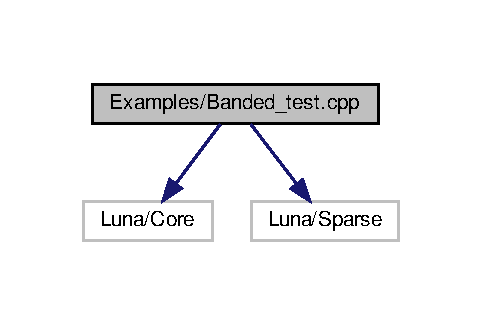
\includegraphics[width=232pt]{Banded__test_8cpp__incl}
\end{center}
\end{figure}
\subsection*{Functions}
\begin{DoxyCompactItemize}
\item 
int \hyperlink{Banded__test_8cpp_ae66f6b31b5ad750f1fe042a706a4e3d4}{main} ()
\end{DoxyCompactItemize}


\subsection{Detailed Description}
T\+O\+DO description / rename file. 



\subsection{Function Documentation}
\mbox{\Hypertarget{Banded__test_8cpp_ae66f6b31b5ad750f1fe042a706a4e3d4}\label{Banded__test_8cpp_ae66f6b31b5ad750f1fe042a706a4e3d4}} 
\index{Banded\+\_\+test.\+cpp@{Banded\+\_\+test.\+cpp}!main@{main}}
\index{main@{main}!Banded\+\_\+test.\+cpp@{Banded\+\_\+test.\+cpp}}
\subsubsection{\texorpdfstring{main()}{main()}}
{\footnotesize\ttfamily int main (\begin{DoxyParamCaption}{ }\end{DoxyParamCaption})}



Definition at line 11 of file Banded\+\_\+test.\+cpp.



References Luna\+::\+Banded\+Matrix$<$ T $>$\+::det(), Luna\+::\+Matrix$<$ T $>$\+::fill\+\_\+band(), Luna\+::\+Banded\+Matrix$<$ T $>$\+::size(), Luna\+::\+Banded\+Matrix$<$ T $>$\+::size\+\_\+above(), Luna\+::\+Banded\+Matrix$<$ T $>$\+::size\+\_\+below(), Luna\+::\+Banded\+Matrix$<$ T $>$\+::solve(), and Heat\+\_\+plot\+::x.



Referenced by Luna\+::\+Tridiagonal$<$ T $>$\+::set\+\_\+main(), and Luna\+::\+Tridiagonal$<$ T $>$\+::\+Tridiagonal().


\begin{DoxyCode}
12 \{
13   cout << \textcolor{stringliteral}{"--------------------- Banded Matrices --------------------"} << endl;
14 
15   std::size\_t n( 4 );
16   \hyperlink{classLuna_1_1Matrix}{Matrix<double>} dense( n, n, 0.0 );
17   dense.fill\_band( -2, 1.0 );
18   dense.fill\_band( -1, 2.0 );
19   dense.fill\_band(  0, 3.0 );
20   dense.fill\_band(  1, 4.0 );
21 
22   cout << \textcolor{stringliteral}{" dense = "} << dense << endl;
23 
24   \textcolor{comment}{// Create a BandedMatrix}
25   std::size\_t bands\_below( 2 );
26   std::size\_t bands\_above( 1 );
27   \hyperlink{classLuna_1_1BandedMatrix}{BandedMatrix<double>} band( dense, bands\_below, bands\_above );
28 
29   cout << \textcolor{stringliteral}{" band = "} << band << endl;
30   \hyperlink{classLuna_1_1Vector}{Vector<double>} b( n, 1.0 );
31   cout << \textcolor{stringliteral}{" b = "} << b << endl;
32   \hyperlink{classLuna_1_1Vector}{Vector<double>} \hyperlink{namespaceHeat__plot_aa88370c16b85b784ccbde3ed88bc1991}{x};
33   x = band.solve( b );
34   cout << \textcolor{stringliteral}{" x = "} << x << endl;
35   cout << \textcolor{stringliteral}{" det = "} << band.det() << endl;
36 
37   cout << \textcolor{stringliteral}{" band.size() = "} << band.\hyperlink{classLuna_1_1Vector_ac9b6ed7a0df401728f27c193fbc8f4d8}{size}() << endl;
38   cout << \textcolor{stringliteral}{" band.size\_below() = "} << band.size\_below() << endl;
39   cout << \textcolor{stringliteral}{" band.size\_above() = "} << band.size\_above() << endl;
40 
41 
42   \textcolor{comment}{//BandedMatrix<double> B( n, bands\_below, bands\_above );}
43   \textcolor{comment}{//B( 0, 0 ) = 17.0;}
44   \textcolor{comment}{//B = band;}
45   \textcolor{comment}{//cout << " B * b = " << B * b << endl;}
46 
47   \hyperlink{classLuna_1_1Matrix}{Matrix<double>} B( n, 2, 1.0 );
48   B( 1, 1 ) = 2.0; B( 2, 1 ) = 3.0; B( 3, 1 ) = 4.0;
49   cout << \textcolor{stringliteral}{" B = "} << B << endl;
50   \hyperlink{classLuna_1_1Matrix}{Matrix<double>} X;
51   X = band.\hyperlink{classLuna_1_1Matrix_abc78c81c129e2bb7ca9f6ee6db2611a9}{solve}( B );
52   cout << \textcolor{stringliteral}{" X = "} << X << endl;
53 
54   \textcolor{comment}{/*typedef std::complex<double> cmplx;}
55 \textcolor{comment}{  Matrix<cmplx> dense\_cmplx( n, n, 0.0 );}
56 \textcolor{comment}{  dense\_cmplx.fill\_band( -2, 1.0 );}
57 \textcolor{comment}{  dense\_cmplx.fill\_band( -1, 2.0 );}
58 \textcolor{comment}{  dense\_cmplx.fill\_band(  0, cmplx( 3.0, 1.0 ) );}
59 \textcolor{comment}{  dense\_cmplx.fill\_band(  1, 4.0 );}
60 \textcolor{comment}{  cout << " dense\_cmplx = " << dense\_cmplx << endl;}
61 \textcolor{comment}{}
62 \textcolor{comment}{  BandedMatrix<cmplx> band\_cmplx( dense\_cmplx, bands\_below, bands\_above );}
63 \textcolor{comment}{  cout << " band\_cmplx = " << band\_cmplx.compact() << endl;}
64 \textcolor{comment}{  Vector<cmplx> b\_cmplx( n, 1.0 );}
65 \textcolor{comment}{  cout << " b\_cmplx = " << b\_cmplx << endl;}
66 \textcolor{comment}{  Vector<cmplx> x\_cmplx;}
67 \textcolor{comment}{  x\_cmplx = band\_cmplx.solve( b\_cmplx );}
68 \textcolor{comment}{  cout << " x\_cmplx = " << x\_cmplx << endl;}
69 \textcolor{comment}{  cout << " det\_cmplx = " << band\_cmplx.det() << endl;*/}
70 
71   cout << \textcolor{stringliteral}{"--- FINISHED ---"} << endl;
72 \}
\end{DoxyCode}

\hypertarget{Eigen__test_8cpp}{}\section{Examples/\+Eigen\+\_\+test.cpp File Reference}
\label{Eigen__test_8cpp}\index{Examples/\+Eigen\+\_\+test.\+cpp@{Examples/\+Eigen\+\_\+test.\+cpp}}


T\+O\+DO description / rename file.  


{\ttfamily \#include \char`\"{}Luna/\+Core\char`\"{}}\newline
{\ttfamily \#include \char`\"{}Luna/\+Eigen\char`\"{}}\newline
{\ttfamily \#include \char`\"{}Luna/\+Sparse\char`\"{}}\newline
Include dependency graph for Eigen\+\_\+test.\+cpp\+:\nopagebreak
\begin{figure}[H]
\begin{center}
\leavevmode
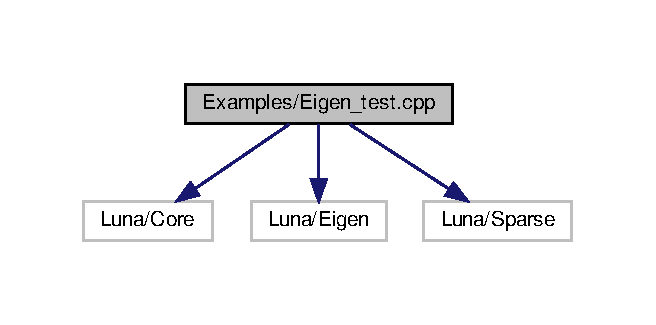
\includegraphics[width=315pt]{Eigen__test_8cpp__incl}
\end{center}
\end{figure}
\subsection*{Functions}
\begin{DoxyCompactItemize}
\item 
int \hyperlink{Eigen__test_8cpp_ae66f6b31b5ad750f1fe042a706a4e3d4}{main} ()
\end{DoxyCompactItemize}


\subsection{Detailed Description}
T\+O\+DO description / rename file. 



\subsection{Function Documentation}
\mbox{\Hypertarget{Eigen__test_8cpp_ae66f6b31b5ad750f1fe042a706a4e3d4}\label{Eigen__test_8cpp_ae66f6b31b5ad750f1fe042a706a4e3d4}} 
\index{Eigen\+\_\+test.\+cpp@{Eigen\+\_\+test.\+cpp}!main@{main}}
\index{main@{main}!Eigen\+\_\+test.\+cpp@{Eigen\+\_\+test.\+cpp}}
\subsubsection{\texorpdfstring{main()}{main()}}
{\footnotesize\ttfamily int main (\begin{DoxyParamCaption}{ }\end{DoxyParamCaption})}



Definition at line 12 of file Eigen\+\_\+test.\+cpp.



References Luna\+::\+Linear\+Eigensystem$<$ T $>$\+::compute\+\_\+real(), Luna\+::\+Linear\+Eigensystem$<$ T $>$\+::compute\+\_\+real\+\_\+symmetric(), Luna\+::\+Linear\+Eigensystem$<$ T $>$\+::compute\+\_\+real\+\_\+symmetric\+\_\+tridiagonal(), Luna\+::\+Linear\+Eigensystem$<$ T $>$\+::eigenvalues(), Luna\+::\+Linear\+Eigensystem$<$ T $>$\+::eigenvector\+\_\+matrix(), Luna\+::\+Linear\+Eigensystem$<$ T $>$\+::eigenvectors(), and Luna\+::\+Vector$<$ T $>$\+::real().


\begin{DoxyCode}
13 \{
14   cout << \textcolor{stringliteral}{"----------------------- Eigensystems ----------------------"} << endl;
15 
16   \hyperlink{classLuna_1_1LinearEigensystem}{LinearEigensystem<double>} eig\_sys;
17 
18   cout << \textcolor{stringliteral}{" * Compute the eigenvalues and eigenvectors of a real"} << endl
19        << \textcolor{stringliteral}{" * symmetric matrix."} << endl;
20 
21   std::size\_t n( 4 );
22   \hyperlink{classLuna_1_1Matrix}{Matrix<double>} A( n, n, 0.0 );
23   \textcolor{comment}{// Lehmer matrix}
24   \textcolor{keywordflow}{for} ( std::size\_t i = 0; i < n; i++ )
25   \{
26     \textcolor{keywordflow}{for} ( std::size\_t j = 0; j < n; j++ )
27     \{
28       \textcolor{keywordflow}{if} ( j >= i )\{
29         A( i, j ) = 1. * ( i + 1 ) / ( j + 1 );
30       \} \textcolor{keywordflow}{else} \{
31         A( i, j ) = 1. * ( j + 1 ) / ( i + 1 );
32       \}
33     \}
34   \}
35 
36   cout << \textcolor{stringliteral}{" * A = "} << A << endl;
37 
38   eig\_sys.\hyperlink{classLuna_1_1LinearEigensystem_ae109e1012fda347ac9c1da4fa30313f6}{compute\_real\_symmetric}( A );
39 
40   cout << \textcolor{stringliteral}{" * evals = "} << eig\_sys.\hyperlink{classLuna_1_1LinearEigensystem_ad74f60a4830eefb2858ab92765dc0ae4}{eigenvalues}().\hyperlink{classLuna_1_1Vector_a39fa58d9f5fdca76b6ffa6cc481f9284}{real}() << endl;
41   cout << \textcolor{stringliteral}{" * evecs = "} << eig\_sys.\hyperlink{classLuna_1_1LinearEigensystem_ab68a36f7f1c1ecf9da83df84be6e49e9}{eigenvector\_matrix}() << endl;
42 
43   \hyperlink{classLuna_1_1Vector}{Vector<double>} evec\_0 = eig\_sys.\hyperlink{classLuna_1_1LinearEigensystem_a34fd0e8eef6dc0e85a13d1cb78beb32f}{eigenvectors}()[ 0 ].real();
44   \textcolor{keywordtype}{double} eval\_0 = eig\_sys.\hyperlink{classLuna_1_1LinearEigensystem_ad74f60a4830eefb2858ab92765dc0ae4}{eigenvalues}().\hyperlink{classLuna_1_1Vector_a39fa58d9f5fdca76b6ffa6cc481f9284}{real}()[ 0 ];
45 
46 
47   cout << \textcolor{stringliteral}{" * A * evec\_0 - eval\_0 * evec\_0 = ["}
48        << A * evec\_0 - eval\_0 * evec\_0 << \textcolor{stringliteral}{"]^T"} << endl;
49 
50   cout << \textcolor{stringliteral}{" * Computer the eigenvalues and eigenvectors of a real "} << endl
51        << \textcolor{stringliteral}{" * symmetric tridiagonal matrix with main diagonal "} << endl;
52   \hyperlink{classLuna_1_1Vector}{Vector<double>} diag( 4, 1.0 );
53   diag[ 0 ] = diag[ 2 ] = 2.0;
54   cout << \textcolor{stringliteral}{" * diag = "} << diag << endl;
55   cout << \textcolor{stringliteral}{" * and off diagonals "} << endl;
56   \hyperlink{classLuna_1_1Vector}{Vector<double>} offdiag( 3, -1.0 );
57   offdiag[ 1 ] = - 2.0; offdiag[ 2 ] = - 3.0;
58   cout << \textcolor{stringliteral}{" * offdiag = "} << offdiag << endl;
59   eig\_sys.\hyperlink{classLuna_1_1LinearEigensystem_a91ac311c3fe4226c4652b6bf41fc0d91}{compute\_real\_symmetric\_tridiagonal}( diag, offdiag );
60   cout << \textcolor{stringliteral}{" * evals = "} << eig\_sys.\hyperlink{classLuna_1_1LinearEigensystem_ad74f60a4830eefb2858ab92765dc0ae4}{eigenvalues}().\hyperlink{classLuna_1_1Vector_a39fa58d9f5fdca76b6ffa6cc481f9284}{real}() << endl;
61   cout << \textcolor{stringliteral}{" * evecs = "} << eig\_sys.\hyperlink{classLuna_1_1LinearEigensystem_ab68a36f7f1c1ecf9da83df84be6e49e9}{eigenvector\_matrix}() << endl;
62 
63   cout << \textcolor{stringliteral}{" * Compute the eigenvalues of a real nonsymmetric matrix. "} << endl;
64   \hyperlink{classLuna_1_1Matrix}{Matrix<double>} B( 3, 3, 1.0 );
65   B( 0, 1 ) = B( 1, 2 ) = B( 2, 0 ) = 2.0;
66   B( 0, 2 ) = B( 1, 0 ) = B( 2, 1 ) = 3.0;
67   cout << \textcolor{stringliteral}{" * B = "} << B << endl;
68 
69   eig\_sys.\hyperlink{classLuna_1_1LinearEigensystem_ab303a80cc2cf6bfe232b9d62efe13109}{compute\_real}( B, \textcolor{keyword}{false} );
70   cout << \textcolor{stringliteral}{" * evals = "} << eig\_sys.\hyperlink{classLuna_1_1LinearEigensystem_ad74f60a4830eefb2858ab92765dc0ae4}{eigenvalues}() << endl;
71 
72 
73   cout << \textcolor{stringliteral}{"--- FINISHED ---"} << endl;
74 \}
\end{DoxyCode}

\hypertarget{Heat__equation_8cpp}{}\section{Examples/\+Heat\+\_\+equation.cpp File Reference}
\label{Heat__equation_8cpp}\index{Examples/\+Heat\+\_\+equation.\+cpp@{Examples/\+Heat\+\_\+equation.\+cpp}}


Solve the heat equation \[ u_t = \alpha u_{xx}, \] where $ \alpha $ is the thermal diffusivity, subject to the boudary conditions $ u(0,t)=u(1,t)=0 $ and the initial condition \[ u(x,0) = u_0(x) = 100 \sin( \pi x ). \] The numerical solution is found using the Crank-\/\+Nicolson method.  


{\ttfamily \#include \char`\"{}Luna/\+Core\char`\"{}}\newline
{\ttfamily \#include \char`\"{}Luna/\+Sparse\char`\"{}}\newline
Include dependency graph for Heat\+\_\+equation.\+cpp\+:\nopagebreak
\begin{figure}[H]
\begin{center}
\leavevmode
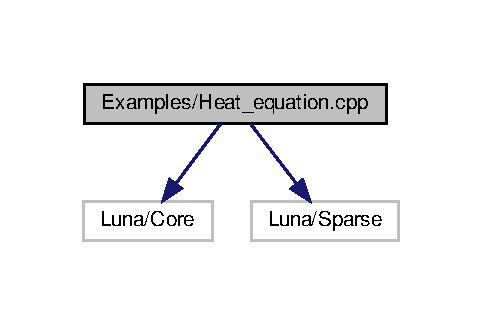
\includegraphics[width=232pt]{Heat__equation_8cpp__incl}
\end{center}
\end{figure}
\subsection*{Functions}
\begin{DoxyCompactItemize}
\item 
int \hyperlink{Heat__equation_8cpp_ae66f6b31b5ad750f1fe042a706a4e3d4}{main} ()
\end{DoxyCompactItemize}


\subsection{Detailed Description}
Solve the heat equation \[ u_t = \alpha u_{xx}, \] where $ \alpha $ is the thermal diffusivity, subject to the boudary conditions $ u(0,t)=u(1,t)=0 $ and the initial condition \[ u(x,0) = u_0(x) = 100 \sin( \pi x ). \] The numerical solution is found using the Crank-\/\+Nicolson method. 



\subsection{Function Documentation}
\mbox{\Hypertarget{Heat__equation_8cpp_ae66f6b31b5ad750f1fe042a706a4e3d4}\label{Heat__equation_8cpp_ae66f6b31b5ad750f1fe042a706a4e3d4}} 
\index{Heat\+\_\+equation.\+cpp@{Heat\+\_\+equation.\+cpp}!main@{main}}
\index{main@{main}!Heat\+\_\+equation.\+cpp@{Heat\+\_\+equation.\+cpp}}
\subsubsection{\texorpdfstring{main()}{main()}}
{\footnotesize\ttfamily int main (\begin{DoxyParamCaption}{ }\end{DoxyParamCaption})}



Definition at line 16 of file Heat\+\_\+equation.\+cpp.



References Heat\+\_\+plot\+::dt, Heat\+\_\+plot\+::J, Luna\+::\+Vector$<$ T $>$\+::linspace(), Heat\+\_\+plot\+::N, Luna\+::\+Mesh2\+D$<$ T $>$\+::output(), Luna\+::\+Tridiagonal$<$ T $>$\+::solve(), and Luna\+::\+Utility\+::stringify().


\begin{DoxyCode}
17 \{
18   cout << \textcolor{stringliteral}{"---------------------- Heat equation ----------------------"} << endl;
19 
20   \textcolor{keywordtype}{double} T\_max( 1.0 );                \textcolor{comment}{// Maximum simulation time}
21   \textcolor{keywordtype}{int} \hyperlink{namespaceHeat__plot_a7d050092798e28458a263710837bda77}{N}( 200 );                       \textcolor{comment}{// Number of time steps}
22   \textcolor{keywordtype}{int} \hyperlink{namespaceHeat__plot_a3cafcec38d886f33b35756791964bb58}{J}( 50 );                        \textcolor{comment}{// Number of spatial steps}
23   \textcolor{keywordtype}{double} \hyperlink{namespaceHeat__plot_ab03c1902ecb064f92219fa9cd5f140d1}{dt}( T\_max / ( 1. * \hyperlink{namespaceHeat__plot_a7d050092798e28458a263710837bda77}{N} ) );    \textcolor{comment}{// Time step}
24   \textcolor{keywordtype}{double} dx( 1.0 / \hyperlink{namespaceHeat__plot_a3cafcec38d886f33b35756791964bb58}{J} );               \textcolor{comment}{// Spatial step}
25   \textcolor{keywordtype}{double} alpha( 1.0 );                \textcolor{comment}{// Thermal diffusivity}
26 
27   cout << \textcolor{stringliteral}{" * Solving the heat equation u\_t = a u\_\{xx\} in the domain"} << endl
28        << \textcolor{stringliteral}{" * t=[0,"} + \hyperlink{namespaceLuna_1_1Utility_a7a21ee8e724765b7a018b6a5394b7e9c}{Utility::stringify}(T\_max) + \textcolor{stringliteral}{"] and x=[0,1] subject to "}
29        << \textcolor{stringliteral}{" the boundary conditions "} << endl << \textcolor{stringliteral}{" * u(0,t)=u(1,t)=0 and the "}
30        << \textcolor{stringliteral}{"initial condition u(x,0)=u\_0(x)."} << endl << \textcolor{stringliteral}{" * The initial "}
31        << \textcolor{stringliteral}{"condition u\_0(x) is specified in the code."}
32        << endl ;
33 
34   cout << \textcolor{stringliteral}{" * The spatial and time steps are:"} << endl;
35   cout << \textcolor{stringliteral}{" * dx = "} << dx << endl;
36   cout << \textcolor{stringliteral}{" * dt = "} << \hyperlink{namespaceHeat__plot_ab03c1902ecb064f92219fa9cd5f140d1}{dt} << endl;
37   cout << \textcolor{stringliteral}{" * and the number of spatial and time steps are:"} << endl;
38   cout << \textcolor{stringliteral}{" * J = "} << \hyperlink{namespaceHeat__plot_a3cafcec38d886f33b35756791964bb58}{J} << endl;
39   cout << \textcolor{stringliteral}{" * N = "} << \hyperlink{namespaceHeat__plot_a7d050092798e28458a263710837bda77}{N} << endl;
40 
41   \textcolor{keywordtype}{double} mu( alpha * \hyperlink{namespaceHeat__plot_ab03c1902ecb064f92219fa9cd5f140d1}{dt} / ( dx * dx ) );
42 
43   \textcolor{comment}{// Mesh for storing the solution}
44   \hyperlink{classLuna_1_1Vector}{Vector<double>} t\_nodes, x\_nodes;
45   t\_nodes.\hyperlink{classLuna_1_1Vector_a275847fc0bddea86c66651201a6db82e}{linspace}( 0.0, T\_max, \hyperlink{namespaceHeat__plot_a7d050092798e28458a263710837bda77}{N} + 1 );
46   x\_nodes.\hyperlink{classLuna_1_1Vector_a275847fc0bddea86c66651201a6db82e}{linspace}( 0.0, 1.0, \hyperlink{namespaceHeat__plot_a3cafcec38d886f33b35756791964bb58}{J} + 1 );
47   \hyperlink{classLuna_1_1Mesh2D}{Mesh2D<double>} solution( x\_nodes, t\_nodes, 1 );
48 
49   \textcolor{comment}{// Matrices for Crank-Nicolson method including BCs u(0,t) = u(1,t) = 0}
50   \hyperlink{classLuna_1_1Tridiagonal}{Tridiagonal<double>} Implicit( -mu, 2. + 2. * mu, -mu, \hyperlink{namespaceHeat__plot_a3cafcec38d886f33b35756791964bb58}{J} + 1 );
51   Implicit( 0, 0 )     = 1.0;
52   Implicit( 0, 1 )     = 0.0;
53   Implicit( \hyperlink{namespaceHeat__plot_a3cafcec38d886f33b35756791964bb58}{J}, \hyperlink{namespaceHeat__plot_a3cafcec38d886f33b35756791964bb58}{J} - 1 ) = 0.0;
54   Implicit( \hyperlink{namespaceHeat__plot_a3cafcec38d886f33b35756791964bb58}{J}, \hyperlink{namespaceHeat__plot_a3cafcec38d886f33b35756791964bb58}{J} )     = 1.0;
55 
56   \hyperlink{classLuna_1_1Tridiagonal}{Tridiagonal<double>} Explicit( mu, 2. - 2. * mu, mu, \hyperlink{namespaceHeat__plot_a3cafcec38d886f33b35756791964bb58}{J} + 1 );
57   Explicit( 0, 0 )     =   1.0;
58   Explicit( 0, 1 )     =   0.0;
59   Explicit( \hyperlink{namespaceHeat__plot_a3cafcec38d886f33b35756791964bb58}{J}, \hyperlink{namespaceHeat__plot_a3cafcec38d886f33b35756791964bb58}{J} - 1 ) =   0.0;
60   Explicit( \hyperlink{namespaceHeat__plot_a3cafcec38d886f33b35756791964bb58}{J}, \hyperlink{namespaceHeat__plot_a3cafcec38d886f33b35756791964bb58}{J} )     = - 1.0;
61 
62   \textcolor{comment}{// Initial condition u\_0(x) = 100 * sin( pi * x )}
63   \hyperlink{classLuna_1_1Vector}{Vector<double>} current( \hyperlink{namespaceHeat__plot_a3cafcec38d886f33b35756791964bb58}{J} + 1, 0.0 );
64   current[ 0 ] = 0.0;
65   solution( 0, 0, 0 ) = current[ 0 ];
66   \textcolor{keywordflow}{for} ( std::size\_t j = 1; j < \hyperlink{namespaceHeat__plot_a3cafcec38d886f33b35756791964bb58}{J}; j++ )
67   \{
68     current[ j ] = 100 * sin( M\_PI * j * dx );
69     solution( j, 0, 0 ) = current[ j ];
70   \}
71   current[ \hyperlink{namespaceHeat__plot_a3cafcec38d886f33b35756791964bb58}{J} ] = 0.0;
72   solution( J, 0, 0 ) = current[ \hyperlink{namespaceHeat__plot_a3cafcec38d886f33b35756791964bb58}{J} ];
73 
74   \hyperlink{classLuna_1_1Vector}{Vector<double>} next( J + 1 );
75 
76   cout << \textcolor{stringliteral}{" * Calculating the solution..."} << endl;
77 
78   \textcolor{keywordflow}{for} ( std::size\_t i = 1; i < \hyperlink{namespaceHeat__plot_a7d050092798e28458a263710837bda77}{N} + 1; i++ )
79   \{
80     current = Explicit * current;
81     next = Implicit.solve( current );
82     current = next;
83     \textcolor{keywordflow}{for} ( std::size\_t j = 0; j < J + 1; j++ )
84     \{
85       solution( j, i, 0 ) = current[ j ];
86     \}
87   \}
88   cout << \textcolor{stringliteral}{" * Solution complete."} << endl;
89 
90   \textcolor{keywordtype}{string} outstring( \textcolor{stringliteral}{"./DATA/Heat\_equation"} );
91   outstring += \textcolor{stringliteral}{"\_J\_"} + \hyperlink{namespaceLuna_1_1Utility_a7a21ee8e724765b7a018b6a5394b7e9c}{Utility::stringify}( J );
92   outstring += \textcolor{stringliteral}{"\_N\_"} + \hyperlink{namespaceLuna_1_1Utility_a7a21ee8e724765b7a018b6a5394b7e9c}{Utility::stringify}( N );
93   outstring += \textcolor{stringliteral}{".dat"};
94   solution.output( outstring );
95 
96   cout << \textcolor{stringliteral}{" * For an animation of the solution run:"} << endl;
97   cout << \textcolor{stringliteral}{"python Plotting/Heat\_plot.py "} << J << \textcolor{stringliteral}{" "} << N << endl;
98   cout << \textcolor{stringliteral}{"--- FINISHED ---"} << endl;
99 \}
\end{DoxyCode}

\hypertarget{Integration_8cpp}{}\section{Examples/\+Integration.cpp File Reference}
\label{Integration_8cpp}\index{Examples/\+Integration.\+cpp@{Examples/\+Integration.\+cpp}}


Some numerical integration examples.  


{\ttfamily \#include \char`\"{}Luna/\+Core\char`\"{}}\newline
Include dependency graph for Integration.\+cpp\+:\nopagebreak
\begin{figure}[H]
\begin{center}
\leavevmode
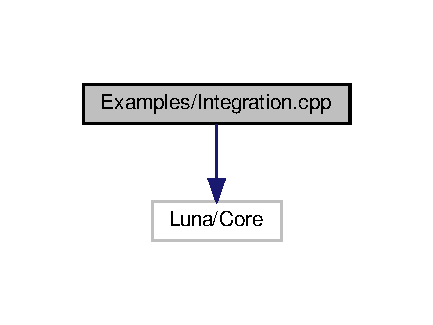
\includegraphics[width=208pt]{Integration_8cpp__incl}
\end{center}
\end{figure}
\subsection*{Functions}
\begin{DoxyCompactItemize}
\item 
int \hyperlink{Integration_8cpp_ae66f6b31b5ad750f1fe042a706a4e3d4}{main} ()
\end{DoxyCompactItemize}


\subsection{Detailed Description}
Some numerical integration examples. 



\subsection{Function Documentation}
\mbox{\Hypertarget{Integration_8cpp_ae66f6b31b5ad750f1fe042a706a4e3d4}\label{Integration_8cpp_ae66f6b31b5ad750f1fe042a706a4e3d4}} 
\index{Integration.\+cpp@{Integration.\+cpp}!main@{main}}
\index{main@{main}!Integration.\+cpp@{Integration.\+cpp}}
\subsubsection{\texorpdfstring{main()}{main()}}
{\footnotesize\ttfamily int main (\begin{DoxyParamCaption}{ }\end{DoxyParamCaption})}



Definition at line 10 of file Integration.\+cpp.



References Luna\+::beta(), Luna\+::\+Mesh1\+D$<$ T, X $>$\+::coord(), Luna\+::\+Mesh2\+D$<$ T $>$\+::coord(), Luna\+::erf(), Luna\+::erfc(), Luna\+::factorial(), Luna\+::gamma(), Luna\+::\+Mesh1\+D$<$ T, X $>$\+::get\+\_\+interpolated\+\_\+vars(), Luna\+::\+Mesh2\+D$<$ T $>$\+::get\+\_\+nnodes(), Luna\+::\+Mesh2\+D$<$ T $>$\+::get\+\_\+nvars(), Luna\+::\+Mesh1\+D$<$ T, X $>$\+::integral(), Luna\+::\+Mesh2\+D$<$ T $>$\+::integral2\+D(), Luna\+::\+Vector$<$ T $>$\+::linspace(), Luna\+::lnfactorial(), Luna\+::lngamma(), Heat\+\_\+plot\+::N, Luna\+::\+Mesh1\+D$<$ T, X $>$\+::nnodes(), Luna\+::\+Mesh1\+D$<$ T, X $>$\+::nvars(), Luna\+::\+Vector$<$ T $>$\+::size(), Heat\+\_\+plot\+::x, y, and Luna\+::\+Bessel$<$ T $>$\+::\+Yn().


\begin{DoxyCode}
11 \{
12   cout << \textcolor{stringliteral}{"----------------- Integration -----------------"} << endl;
13   cout << \textcolor{stringliteral}{"  * Create a 1D mesh with 2 variables and set "}  << endl;
14   cout << \textcolor{stringliteral}{"  * one equal 2x and the other to x^2. "}  << endl;
15 
16   \hyperlink{classLuna_1_1Vector}{Vector<double>} nodes;
17   nodes.\hyperlink{classLuna_1_1Vector_a275847fc0bddea86c66651201a6db82e}{linspace}( 0, 1, 101 );
18   std::size\_t nvars( 2 );
19   \hyperlink{classLuna_1_1Mesh1D}{Mesh1D<double>} mesh( nodes, nvars );
20 
21   \textcolor{keywordflow}{for} ( std::size\_t i = 0; i< nodes.\hyperlink{classLuna_1_1Vector_ac9b6ed7a0df401728f27c193fbc8f4d8}{size}(); ++i )
22   \{
23     \textcolor{keywordtype}{double} \hyperlink{namespaceHeat__plot_aa88370c16b85b784ccbde3ed88bc1991}{x}( mesh.coord( i ) );
24     mesh( i, 0 ) = 2 * \hyperlink{namespaceHeat__plot_aa88370c16b85b784ccbde3ed88bc1991}{x};
25     mesh( i, 1 ) = \hyperlink{namespaceHeat__plot_aa88370c16b85b784ccbde3ed88bc1991}{x} * \hyperlink{namespaceHeat__plot_aa88370c16b85b784ccbde3ed88bc1991}{x};
26   \}
27 
28   cout << \textcolor{stringliteral}{"  * # nodes = "} << mesh.nnodes() << endl;
29   cout << \textcolor{stringliteral}{"  * # variables = "} << mesh.nvars() << endl;
30   \hyperlink{classLuna_1_1Vector}{Vector<double>} vars;
31   vars = mesh.get\_interpolated\_vars( 0.35 );
32   cout << \textcolor{stringliteral}{"  * Interpolate the values of each of the "} << endl;
33   cout << \textcolor{stringliteral}{"  * variables at a specified point."} << endl;
34 
35   cout << \textcolor{stringliteral}{"  * vars( 0.35 ) = "} << vars << endl;
36 
37   cout << \textcolor{stringliteral}{"  * Numerically integrate the variables over "} << endl;
38   cout << \textcolor{stringliteral}{"  * the domain (from 0 to 1). "} << endl;
39 
40   cout << \textcolor{stringliteral}{"  * mesh.integral( 0 ) = "} << mesh.integral( 0 ) << endl;
41   cout << \textcolor{stringliteral}{"  * mesh.integral( 1 ) = "} << mesh.integral( 1 ) << endl;
42 
43   cout << \textcolor{stringliteral}{"-----------------------------------------------"} << endl;
44   cout << \textcolor{stringliteral}{"  * Create a 2D mesh with 2 variables and set "}  << endl;
45   cout << \textcolor{stringliteral}{"  * one equal 2x^2 and the other to 3y. "}  << endl;
46   cout << \textcolor{stringliteral}{"  * The domain is split uniformly from 0 to 1."} << endl;
47 
48   std::size\_t \hyperlink{namespaceHeat__plot_a7d050092798e28458a263710837bda77}{N}( 101 );
49   \hyperlink{classLuna_1_1Vector}{Vector<double>} x\_nodes, y\_nodes;
50   x\_nodes.\hyperlink{classLuna_1_1Vector_a275847fc0bddea86c66651201a6db82e}{linspace}( 0, 1, \hyperlink{namespaceHeat__plot_a7d050092798e28458a263710837bda77}{N} );
51   y\_nodes.\hyperlink{classLuna_1_1Vector_a275847fc0bddea86c66651201a6db82e}{linspace}( 0, 1, \hyperlink{namespaceHeat__plot_a7d050092798e28458a263710837bda77}{N} );
52   \hyperlink{classLuna_1_1Mesh2D}{Mesh2D<double>} mesh2d( x\_nodes, y\_nodes, nvars );
53 
54   \textcolor{keywordflow}{for} ( std::size\_t i = 0; i < x\_nodes.\hyperlink{classLuna_1_1Vector_ac9b6ed7a0df401728f27c193fbc8f4d8}{size}(); ++i )
55   \{
56     \textcolor{keywordflow}{for} ( std::size\_t j = 0; j < y\_nodes.\hyperlink{classLuna_1_1Vector_ac9b6ed7a0df401728f27c193fbc8f4d8}{size}(); ++j )
57     \{
58       \textcolor{keywordtype}{double} \hyperlink{namespaceHeat__plot_aa88370c16b85b784ccbde3ed88bc1991}{x}( mesh2d.coord( i, j ).first );
59       \textcolor{keywordtype}{double} \hyperlink{ODE__BVP__test_8cpp_adf764cbdea00d65edcd07bb9953ad2b7ae1f9fdb8b786c63efc4ce44eeacd17f2}{y}( mesh2d.coord( i, j ).second );
60       mesh2d( i, j, 0 ) = 2 * \hyperlink{namespaceHeat__plot_aa88370c16b85b784ccbde3ed88bc1991}{x} * \hyperlink{namespaceHeat__plot_aa88370c16b85b784ccbde3ed88bc1991}{x};
61       mesh2d( i, j, 1 ) = 3 * \hyperlink{ODE__BVP__test_8cpp_adf764cbdea00d65edcd07bb9953ad2b7ae1f9fdb8b786c63efc4ce44eeacd17f2}{y};
62     \}
63   \}
64 
65   cout << \textcolor{stringliteral}{"  * # x nodes = "} << mesh2d.get\_nnodes().first << endl;
66   cout << \textcolor{stringliteral}{"  * # y nodes = "} << mesh2d.get\_nnodes().second << endl;
67   cout << \textcolor{stringliteral}{"  * # variables = "} << mesh2d.get\_nvars() << endl;
68   cout << \textcolor{stringliteral}{"  * Integrate each variable over the domain."} << endl;
69   cout << \textcolor{stringliteral}{"  * mesh2d.integral2D( 0 ) = "} << mesh2d.integral2D( 0 ) << endl;
70   cout << \textcolor{stringliteral}{"  * mesh2d.integral2D( 1 ) = "} << mesh2d.integral2D( 1 ) << endl;
71   cout << \textcolor{stringliteral}{"-----------------------------------------------"} << endl;
72 
73   std::complex<double> \hyperlink{namespaceHeat__plot_aa88370c16b85b784ccbde3ed88bc1991}{x}( 1.0 / 3.0, 1.0 );
74   cout << \textcolor{stringliteral}{" gamma( 1/3 + i ) = "} << std::setprecision( 8 )
75        << \hyperlink{namespaceLuna_a4467788060a97debe131fa8f08a00de3}{Luna::gamma}( \hyperlink{namespaceHeat__plot_aa88370c16b85b784ccbde3ed88bc1991}{x} ) << endl;
76 
77   cout << \textcolor{stringliteral}{" lngamma( 0.5 ) = "} << std::setprecision( 6 )
78        << \hyperlink{namespaceLuna_a5682d79a57f8eb7e6c08654af8955d4c}{Luna::lngamma}( 0.5 ) << endl;
79 
80   cout << \textcolor{stringliteral}{" factorial( 5 ) = "} << \hyperlink{namespaceLuna_a62f1af647be5ca8909ba79911afede93}{Luna::factorial}( 5 ) << endl;
81   cout << \textcolor{stringliteral}{" lnfactorial( 5000 ) = "} << \hyperlink{namespaceLuna_af55fcfd16fe0fd817853f43623de1ea5}{Luna::lnfactorial}( 5000 ) << endl;
82   cout << \textcolor{stringliteral}{" beta( 5, 4 ) = "} << \hyperlink{namespaceLuna_af542f1c7522ca96017105e160b54df80}{Luna::beta}( 5., 4. ) << endl;
83   std::complex<double> z( 0.1, 1.0 );
84   cout << \textcolor{stringliteral}{" erf( 0.1 + i ) = "} << \hyperlink{namespaceLuna_a297d1af9ebec3d1b70600f28ff78f137}{Luna::erf}( z ) << endl;
85   cout << \textcolor{stringliteral}{" erfc( 0.1 + i ) = "} << \hyperlink{namespaceLuna_aa9ceeb6a99e1f82aa1d4614bcc9653be}{Luna::erfc}( z ) << endl;
86   \hyperlink{structLuna_1_1Bessel}{Luna::Bessel<std::complex<double>}> bessel;
87   z.real( 1.0 );
88   cout << \textcolor{stringliteral}{" Y2( 1 + i ) = "} << bessel.\hyperlink{structLuna_1_1Bessel_aeffbc7ae897573b756c0ddab93ecf6de}{Yn}( 2, z ) << endl;
89 
90 
91 
92   cout << \textcolor{stringliteral}{"--- FINISHED ---"} << endl;
93 
94 \}
\end{DoxyCode}

\hypertarget{Laplace__equation_8cpp}{}\section{Examples/\+Laplace\+\_\+equation.cpp File Reference}
\label{Laplace__equation_8cpp}\index{Examples/\+Laplace\+\_\+equation.\+cpp@{Examples/\+Laplace\+\_\+equation.\+cpp}}


Solve Laplace\textquotesingle{}s equation \[ \nabla^2 u = 0, \] on the unit square $ (x,y) \in [0,1] \times [0,1] $.  


{\ttfamily \#include \char`\"{}Luna/\+Core\char`\"{}}\newline
{\ttfamily \#include \char`\"{}Luna/\+Sparse\char`\"{}}\newline
Include dependency graph for Laplace\+\_\+equation.\+cpp\+:\nopagebreak
\begin{figure}[H]
\begin{center}
\leavevmode
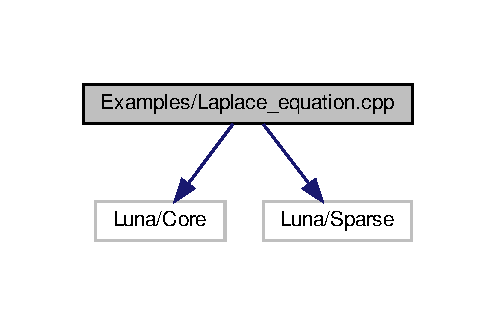
\includegraphics[width=238pt]{Laplace__equation_8cpp__incl}
\end{center}
\end{figure}
\subsection*{Functions}
\begin{DoxyCompactItemize}
\item 
int \hyperlink{Laplace__equation_8cpp_ae66f6b31b5ad750f1fe042a706a4e3d4}{main} ()
\end{DoxyCompactItemize}


\subsection{Detailed Description}
Solve Laplace\textquotesingle{}s equation \[ \nabla^2 u = 0, \] on the unit square $ (x,y) \in [0,1] \times [0,1] $. 

The equation is subject to the boundary conditions \[ u(x,0) = 0, \hspace{0.5cm} u(x,1) = \frac{1}{(1+x)^2 + 1}, \hspace{0.5cm} 0 \leq x \leq 1, \] \[ u(0,y) = \frac{y}{1+y^2}, \hspace{0.5cm} u(1,y) = \frac{y}{4+y^2}, \hspace{0.5cm} 0 \leq y \leq 1. \] The exact solution is given by \[ u(x,y) = \frac{y}{(1+x)^2 + y^2}, \hspace{0.5cm} 0 \leq x,y \leq 1. \] The equation is discretised using a second order finite-\/difference scheme with step size $ \Delta x = \Delta y = 1 / N $ where $ N $ is the number of intervals. The internal nodes in the discretisation are governed by the finite-\/difference equation \[ u_{i-1,j} + u_{i,j-1} - 4u_{i,j} + u_{i,j+1} + u_{i+1,j} = 0, \] where $ u(x,y) \approx u(x_i,y_j) = u_{i,j} $ and $ x_i = i \Delta x, \hspace{0.2cm} y_j = j \Delta y $ with $ i,j = 0,1,\ldots,N. $ 

\subsection{Function Documentation}
\mbox{\Hypertarget{Laplace__equation_8cpp_ae66f6b31b5ad750f1fe042a706a4e3d4}\label{Laplace__equation_8cpp_ae66f6b31b5ad750f1fe042a706a4e3d4}} 
\index{Laplace\+\_\+equation.\+cpp@{Laplace\+\_\+equation.\+cpp}!main@{main}}
\index{main@{main}!Laplace\+\_\+equation.\+cpp@{Laplace\+\_\+equation.\+cpp}}
\subsubsection{\texorpdfstring{main()}{main()}}
{\footnotesize\ttfamily int main (\begin{DoxyParamCaption}{ }\end{DoxyParamCaption})}



Definition at line 24 of file Laplace\+\_\+equation.\+cpp.



References Luna\+::\+Timer\+::get\+\_\+time(), Heat\+\_\+plot\+::N, Luna\+::\+Vector$<$ T $>$\+::norm\+\_\+2(), Luna\+::\+Vector$<$ T $>$\+::random(), Luna\+::\+Sparse\+Matrix$<$ T $>$\+::solve\+\_\+\+Bi\+C\+G(), Luna\+::\+Timer\+::start(), Luna\+::\+Timer\+::stop(), Heat\+\_\+plot\+::u, Heat\+\_\+plot\+::x, and y.


\begin{DoxyCode}
25 \{
26   cout << \textcolor{stringliteral}{"--------------------- Laplace's equation --------------------"} << endl;
27 
28   \textcolor{keywordtype}{int} \hyperlink{namespaceHeat__plot_a7d050092798e28458a263710837bda77}{N}( 256 );                              \textcolor{comment}{// Number of intervals}
29   \textcolor{keywordtype}{double} dx( 1.0 / \hyperlink{namespaceHeat__plot_a7d050092798e28458a263710837bda77}{N} );                      \textcolor{comment}{// Step size}
30   std::size\_t size( ( \hyperlink{namespaceHeat__plot_a7d050092798e28458a263710837bda77}{N} + 1 ) * ( \hyperlink{namespaceHeat__plot_a7d050092798e28458a263710837bda77}{N} + 1 ) ); \textcolor{comment}{// Size of the linear system}
31   \hyperlink{classLuna_1_1Vector}{Vector<double>} rhs( size, 0.0 );           \textcolor{comment}{// Right hand side vector}
32   \hyperlink{classLuna_1_1Vector}{Vector<double>} \hyperlink{namespaceHeat__plot_ae622b86afa46daa3e9b887624ab1bf26}{u}( size, 0.0 );             \textcolor{comment}{// Solution vector}
33   \hyperlink{classLuna_1_1Vector}{Vector<double>} u\_exact( size, 0.0 );       \textcolor{comment}{// Exact solution}
34 
35   \textcolor{keyword}{typedef} \hyperlink{classLuna_1_1Triplet}{Triplet<double>} Td;
36   \hyperlink{classLuna_1_1Vector}{Vector<Td>} triplets;
37 
38   \textcolor{keywordtype}{double} \hyperlink{namespaceHeat__plot_aa88370c16b85b784ccbde3ed88bc1991}{x}( 0.0 );
39   \textcolor{keywordtype}{double} \hyperlink{ODE__BVP__test_8cpp_adf764cbdea00d65edcd07bb9953ad2b7ae1f9fdb8b786c63efc4ce44eeacd17f2}{y}( 0.0 );
40   std::size\_t row( 0 );
41 
42   \textcolor{comment}{// x = 0 boundary ( u = y / ( 1 + y^2 ) )}
43   std::size\_t i( 0 );
44   std::size\_t j( 0 );
45   \textcolor{keywordflow}{for} ( j = 0; j < \hyperlink{namespaceHeat__plot_a7d050092798e28458a263710837bda77}{N} + 1; j++ )
46   \{
47     \hyperlink{ODE__BVP__test_8cpp_adf764cbdea00d65edcd07bb9953ad2b7ae1f9fdb8b786c63efc4ce44eeacd17f2}{y} = j * dx;
48     triplets( Td( row, i * ( N + 1 ) + j, 1.0 ) );
49     rhs[ row ] = \hyperlink{ODE__BVP__test_8cpp_adf764cbdea00d65edcd07bb9953ad2b7ae1f9fdb8b786c63efc4ce44eeacd17f2}{y} / ( 1 + \hyperlink{ODE__BVP__test_8cpp_adf764cbdea00d65edcd07bb9953ad2b7ae1f9fdb8b786c63efc4ce44eeacd17f2}{y} * \hyperlink{ODE__BVP__test_8cpp_adf764cbdea00d65edcd07bb9953ad2b7ae1f9fdb8b786c63efc4ce44eeacd17f2}{y} );
50     ++row;
51   \}
52 
53   \textcolor{keywordflow}{for} ( i = 1; i < \hyperlink{namespaceHeat__plot_a7d050092798e28458a263710837bda77}{N}; i++ )
54   \{
55     \hyperlink{namespaceHeat__plot_aa88370c16b85b784ccbde3ed88bc1991}{x} = i * dx;
56     \textcolor{comment}{// y = 0 boundary ( u = 0 )}
57     j = 0;
58     triplets( Td( row, i * ( N + 1 ) + j, 1.0 ) );
59     rhs[ row ] = 0.0;
60     ++row;
61     \textcolor{comment}{// Interior nodes}
62     \textcolor{keywordflow}{for} ( j = 1; j < \hyperlink{namespaceHeat__plot_a7d050092798e28458a263710837bda77}{N}; j++ )
63     \{
64       triplets( Td( row, ( i - 1 ) * ( N + 1 ) + j, 1.0 ) );
65       triplets( Td( row, ( i + 1 ) * ( N + 1 ) + j, 1.0 ) );
66       triplets( Td( row, i * ( N + 1 ) + j - 1, 1.0 ) );
67       triplets( Td( row, i * ( N + 1 ) + j + 1, 1.0 ) );
68       triplets( Td( row, i * ( N + 1 ) + j, - 4.0 ) );
69       rhs[ row ] = 0.0;
70       ++row;
71     \}
72     \textcolor{comment}{// y = 1 boundary ( u = 1 / ( ( 1 + x )^2 + 1 ) )}
73     j = \hyperlink{namespaceHeat__plot_a7d050092798e28458a263710837bda77}{N};
74     triplets( Td( row, i * ( N + 1 ) + j, 1.0 ) );
75     rhs[ row ] = 1. / ( ( 1. + \hyperlink{namespaceHeat__plot_aa88370c16b85b784ccbde3ed88bc1991}{x} ) * ( 1. + \hyperlink{namespaceHeat__plot_aa88370c16b85b784ccbde3ed88bc1991}{x} ) + 1. );
76     ++row;
77   \}
78 
79   \textcolor{comment}{// x = 1 boundary ( u = y / ( 4 + y^2 ) )}
80   i = \hyperlink{namespaceHeat__plot_a7d050092798e28458a263710837bda77}{N};
81   \textcolor{keywordflow}{for} ( j = 0; j < N + 1; j++ )
82   \{
83     \hyperlink{ODE__BVP__test_8cpp_adf764cbdea00d65edcd07bb9953ad2b7ae1f9fdb8b786c63efc4ce44eeacd17f2}{y} = j * dx;
84     triplets( Td( row, i * ( N + 1 ) + j, 1.0 ) );
85     rhs[ row ] = \hyperlink{ODE__BVP__test_8cpp_adf764cbdea00d65edcd07bb9953ad2b7ae1f9fdb8b786c63efc4ce44eeacd17f2}{y} / ( 4 + \hyperlink{ODE__BVP__test_8cpp_adf764cbdea00d65edcd07bb9953ad2b7ae1f9fdb8b786c63efc4ce44eeacd17f2}{y} * \hyperlink{ODE__BVP__test_8cpp_adf764cbdea00d65edcd07bb9953ad2b7ae1f9fdb8b786c63efc4ce44eeacd17f2}{y} );
86     ++row;
87   \}
88 
89   \textcolor{comment}{// Exact solution u = y / ( ( 1 + x )^2 + y^2 )}
90   row = 0;
91   \textcolor{keywordflow}{for} ( i = 0; i < N + 1; i++ )
92   \{
93     \hyperlink{namespaceHeat__plot_aa88370c16b85b784ccbde3ed88bc1991}{x} = i * dx;
94     \textcolor{keywordflow}{for} ( j = 0; j < N + 1; j++ )
95     \{
96       \hyperlink{ODE__BVP__test_8cpp_adf764cbdea00d65edcd07bb9953ad2b7ae1f9fdb8b786c63efc4ce44eeacd17f2}{y} = j * dx;
97       u\_exact[ row ] = \hyperlink{ODE__BVP__test_8cpp_adf764cbdea00d65edcd07bb9953ad2b7ae1f9fdb8b786c63efc4ce44eeacd17f2}{y} / ( ( 1. + \hyperlink{namespaceHeat__plot_aa88370c16b85b784ccbde3ed88bc1991}{x} ) * ( 1. + \hyperlink{namespaceHeat__plot_aa88370c16b85b784ccbde3ed88bc1991}{x} ) + \hyperlink{ODE__BVP__test_8cpp_adf764cbdea00d65edcd07bb9953ad2b7ae1f9fdb8b786c63efc4ce44eeacd17f2}{y} * \hyperlink{ODE__BVP__test_8cpp_adf764cbdea00d65edcd07bb9953ad2b7ae1f9fdb8b786c63efc4ce44eeacd17f2}{y} );
98       ++row;
99     \}
100   \}
101 
102   \textcolor{comment}{// Create the sparse matrix from the triplets}
103   \hyperlink{classLuna_1_1SparseMatrix}{SparseMatrix<double>} sparse( size, size, triplets );
104 
105   \textcolor{comment}{// Solve using the Biconjugate gradient method}
106   \hyperlink{namespaceHeat__plot_ae622b86afa46daa3e9b887624ab1bf26}{u}.random();                                    \textcolor{comment}{// Random initial guess}
107   \textcolor{keywordtype}{double} tol( 1e-8 );
108   \textcolor{keywordtype}{int} code;
109   \textcolor{keywordtype}{int} max\_iter( 10000 );
110 
111   \hyperlink{classLuna_1_1Timer}{Timer} timer;
112   \textcolor{keywordtype}{double} time\_in\_ms;
113   timer.\hyperlink{classLuna_1_1Timer_ab074740a502b02be0bb64ef3320733b3}{start}();
114   code = sparse.solve\_BiCG( rhs, \hyperlink{namespaceHeat__plot_ae622b86afa46daa3e9b887624ab1bf26}{u}, max\_iter, tol );
115   time\_in\_ms = timer.\hyperlink{classLuna_1_1Timer_ac8b59a9f3d149ec56156af6f74a6d1a9}{get\_time}();
116   timer.\hyperlink{classLuna_1_1Timer_ad8ba9deb09bfe422cfaadba04a776662}{stop}();
117 
118   cout << endl << \textcolor{stringliteral}{" * time = "} << time\_in\_ms / 1000 << \textcolor{stringliteral}{" s"} << endl;
119   cout << \textcolor{stringliteral}{" * iter = "} << max\_iter << endl;
120   cout << \textcolor{stringliteral}{" * system error estimate = "} << scientific << tol << endl;
121   \hyperlink{namespaceHeat__plot_ae622b86afa46daa3e9b887624ab1bf26}{u} = \hyperlink{namespaceHeat__plot_ae622b86afa46daa3e9b887624ab1bf26}{u} - u\_exact;
122   cout << \textcolor{stringliteral}{" * solution error = "} << \hyperlink{namespaceHeat__plot_ae622b86afa46daa3e9b887624ab1bf26}{u}.norm\_2() << endl;
123   cout << \textcolor{stringliteral}{" * code ( 0 = success ) = "} << code << endl << endl;
124   cout << \textcolor{stringliteral}{"--- FINISHED ---"} << endl;
125 \}
\end{DoxyCode}

\hypertarget{Linear__system_8cpp}{}\section{Examples/\+Linear\+\_\+system.cpp File Reference}
\label{Linear__system_8cpp}\index{Examples/\+Linear\+\_\+system.\+cpp@{Examples/\+Linear\+\_\+system.\+cpp}}


Solve some linear systems of equations.  


{\ttfamily \#include \char`\"{}Luna/\+Core\char`\"{}}\newline
Include dependency graph for Linear\+\_\+system.\+cpp\+:\nopagebreak
\begin{figure}[H]
\begin{center}
\leavevmode
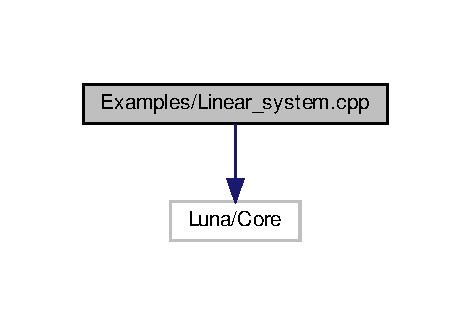
\includegraphics[width=226pt]{Linear__system_8cpp__incl}
\end{center}
\end{figure}
\subsection*{Functions}
\begin{DoxyCompactItemize}
\item 
int \hyperlink{Linear__system_8cpp_a3c04138a5bfe5d72780bb7e82a18e627}{main} (int argc, char $\ast$$\ast$argv)
\end{DoxyCompactItemize}


\subsection{Detailed Description}
Solve some linear systems of equations. 



\subsection{Function Documentation}
\mbox{\Hypertarget{Linear__system_8cpp_a3c04138a5bfe5d72780bb7e82a18e627}\label{Linear__system_8cpp_a3c04138a5bfe5d72780bb7e82a18e627}} 
\index{Linear\+\_\+system.\+cpp@{Linear\+\_\+system.\+cpp}!main@{main}}
\index{main@{main}!Linear\+\_\+system.\+cpp@{Linear\+\_\+system.\+cpp}}
\subsubsection{\texorpdfstring{main()}{main()}}
{\footnotesize\ttfamily int main (\begin{DoxyParamCaption}\item[{int}]{argc,  }\item[{char $\ast$$\ast$}]{argv }\end{DoxyParamCaption})}



Definition at line 10 of file Linear\+\_\+system.\+cpp.



References Luna\+::\+Matrix$<$ T $>$\+::det(), Luna\+::\+Timer\+::get\+\_\+time(), Luna\+::\+Matrix$<$ T $>$\+::inverse(), Luna\+::\+Matrix$<$ T $>$\+::\+L\+U\+\_\+decomp(), Heat\+\_\+plot\+::N, Luna\+::\+Matrix$<$ T $>$\+::random(), Luna\+::\+Vector$<$ T $>$\+::resize(), Luna\+::\+Matrix$<$ T $>$\+::resize(), Luna\+::\+Matrix$<$ T $>$\+::solve\+\_\+basic(), Luna\+::\+Timer\+::start(), Luna\+::\+Timer\+::stop(), Heat\+\_\+plot\+::x, and y.


\begin{DoxyCode}
11 \{
12   cout << \textcolor{stringliteral}{"---------------- Linear system ----------------"} << endl;
13 
14   \hyperlink{classLuna_1_1Matrix}{Matrix<double>} A( 3, 3, 0.0 );
15   \hyperlink{classLuna_1_1Vector}{Vector<double>} b( 3, 0.0 );
16   \hyperlink{classLuna_1_1Vector}{Vector<double>} \hyperlink{namespaceHeat__plot_aa88370c16b85b784ccbde3ed88bc1991}{x};
17 
18   cout << \textcolor{stringliteral}{"  * Solve the linear system Ax=b for x where"} << endl;
19 
20   A( 0, 0 ) = 1.0; A( 0, 1 ) = 1.0; A( 0, 2 ) =   1.0;
21   A( 1, 0 ) = 0.0; A( 1, 1 ) = 2.0; A( 1, 2 ) =   5.0;
22   A( 2, 0 ) = 2.0; A( 2, 1 ) = 5.0; A( 2, 2 ) = - 1.0;
23   cout << \textcolor{stringliteral}{"  * A = "} << A << endl;
24 
25   b[ 0 ] = 6.0; b[ 1 ] = - 4.0; b[ 2 ] = 27.0;
26   cout << \textcolor{stringliteral}{"  * b^T = "} << b << endl;
27   cout << \textcolor{stringliteral}{"  * gives the solution vector "} << endl;
28 
29   x = A.solve\_basic( b );
30   cout << \textcolor{stringliteral}{"  * x^T = "} << x << endl;
31 
32   cout << \textcolor{stringliteral}{"-----------------------------------------------"} << endl;
33 
34   cout << \textcolor{stringliteral}{"  * Solve the complex linear system CX=B for X "} << endl;
35   cout << \textcolor{stringliteral}{"  * where C, X and B are complex matrices. "} << endl;
36 
37   \hyperlink{classLuna_1_1Matrix}{Matrix< std::complex<double>} > C( 2, 2, 0.0 );
38   \hyperlink{classLuna_1_1Matrix}{Matrix< std::complex<double>} > B( 2, 3, 0.0 );
39   \hyperlink{classLuna_1_1Matrix}{Matrix< std::complex<double>} > X( 2, 3, 0.0 );
40 
41   C.random();
42   cout << \textcolor{stringliteral}{"  * C = "} << C << endl;
43 
44   B.random();
45   cout << \textcolor{stringliteral}{"  * B = "} << B << endl;
46 
47   cout << \textcolor{stringliteral}{"  * gives the solution matrix "} << endl;
48   X = C.solve\_basic( B );
49   cout << \textcolor{stringliteral}{"  * X = "} << X << endl;
50 
51   cout << \textcolor{stringliteral}{"  * This solution may easily be checked i.e. "} << endl;
52   cout << \textcolor{stringliteral}{"  * CX - B = "} << C * X - B << endl;
53 
54   cout << \textcolor{stringliteral}{"-----------------------------------------------"} << endl;
55 
56   cout << \textcolor{stringliteral}{"  * In theory we may solve systems of any size"} << endl;
57   cout << \textcolor{stringliteral}{"  * but in practice this can be time consuming. "} << endl;
58 
59   \hyperlink{classLuna_1_1Timer}{Timer} timer;
60   \textcolor{keywordtype}{double} time\_in\_ms;
61   std::size\_t \hyperlink{namespaceHeat__plot_a7d050092798e28458a263710837bda77}{N}( 16 );
62   \hyperlink{classLuna_1_1Matrix}{Matrix<double>} D( \hyperlink{namespaceHeat__plot_a7d050092798e28458a263710837bda77}{N}, \hyperlink{namespaceHeat__plot_a7d050092798e28458a263710837bda77}{N}, 0.0 );
63 
64   cout << \textcolor{stringliteral}{"  * For example: "} << endl;
65 
66   \textcolor{keywordflow}{for} ( std::size\_t i = 0; i < 7; ++i )
67   \{
68     D.resize( \hyperlink{namespaceHeat__plot_a7d050092798e28458a263710837bda77}{N}, \hyperlink{namespaceHeat__plot_a7d050092798e28458a263710837bda77}{N} );
69     D.random();
70     x.\hyperlink{classLuna_1_1Vector_ae1394f960d5cac3e60f6b1561f38e453}{resize}( \hyperlink{namespaceHeat__plot_a7d050092798e28458a263710837bda77}{N} );
71     \hyperlink{classLuna_1_1Vector}{Vector<double>} \hyperlink{ODE__BVP__test_8cpp_adf764cbdea00d65edcd07bb9953ad2b7ae1f9fdb8b786c63efc4ce44eeacd17f2}{y}( \hyperlink{namespaceHeat__plot_a7d050092798e28458a263710837bda77}{N}, 1.0 );
72 
73     timer.\hyperlink{classLuna_1_1Timer_ab074740a502b02be0bb64ef3320733b3}{start}();
74     x = D.solve\_basic( \hyperlink{ODE__BVP__test_8cpp_adf764cbdea00d65edcd07bb9953ad2b7ae1f9fdb8b786c63efc4ce44eeacd17f2}{y} );
75     time\_in\_ms = timer.\hyperlink{classLuna_1_1Timer_ac8b59a9f3d149ec56156af6f74a6d1a9}{get\_time}();
76     timer.\hyperlink{classLuna_1_1Timer_ad8ba9deb09bfe422cfaadba04a776662}{stop}();
77 
78     cout << \textcolor{stringliteral}{"  * solving a "} << \hyperlink{namespaceHeat__plot_a7d050092798e28458a263710837bda77}{N} << \textcolor{stringliteral}{"x"} << \hyperlink{namespaceHeat__plot_a7d050092798e28458a263710837bda77}{N} << \textcolor{stringliteral}{" system takes "}
79          << time\_in\_ms << \textcolor{stringliteral}{" ms. "} << endl;
80     \hyperlink{namespaceHeat__plot_a7d050092798e28458a263710837bda77}{N} *= 2;
81   \}
82 
83   cout << \textcolor{stringliteral}{"-----------------------------------------------"} << endl;
84   cout << \textcolor{stringliteral}{"  * Calculate the LU decomposition of a 3x3  "} << endl;
85   cout << \textcolor{stringliteral}{"  * matrix with partial pivoting ( PA = LU )."} << endl;
86   A( 0, 0 ) = 2.0; A( 0, 1 ) =   4.0; A( 0, 2 ) =  1.0;
87   A( 1, 0 ) = 4.0; A( 1, 1 ) = -10.0; A( 1, 2 ) =  2.0;
88   A( 2, 0 ) = 1.0; A( 2, 1 ) =   2.0; A( 2, 2 ) =  4.0;
89   \hyperlink{namespaceHeat__plot_a7d050092798e28458a263710837bda77}{N} = 3;
90   cout << \textcolor{stringliteral}{"  * A = "} << A << endl;
91 
92   \hyperlink{classLuna_1_1Matrix}{Matrix<double>} L( \hyperlink{namespaceHeat__plot_a7d050092798e28458a263710837bda77}{N}, \hyperlink{namespaceHeat__plot_a7d050092798e28458a263710837bda77}{N}, 0.0 );
93   \hyperlink{classLuna_1_1Matrix}{Matrix<double>} U( \hyperlink{namespaceHeat__plot_a7d050092798e28458a263710837bda77}{N}, \hyperlink{namespaceHeat__plot_a7d050092798e28458a263710837bda77}{N}, 0.0 );
94   \hyperlink{classLuna_1_1Matrix}{Matrix<double>} P( \hyperlink{namespaceHeat__plot_a7d050092798e28458a263710837bda77}{N}, \hyperlink{namespaceHeat__plot_a7d050092798e28458a263710837bda77}{N}, 0.0 );
95 
96   A.LU\_decomp( L, U, P );
97 
98   cout << \textcolor{stringliteral}{"  * L = "} << L << endl;
99   cout << \textcolor{stringliteral}{"  * U = "} << U << endl;
100   cout << \textcolor{stringliteral}{"  * P = "} << P << endl;
101   cout << \textcolor{stringliteral}{"  * Check that the decomposition has worked."} << endl;
102   cout << \textcolor{stringliteral}{"  * PA - LU = "} << P * A - L * U << endl;
103   cout << \textcolor{stringliteral}{"  * Now caluculate the determinant of the matrix."} << endl;
104   cout << \textcolor{stringliteral}{"  * A.det() = "} << A.det() << endl;
105   \hyperlink{classLuna_1_1Matrix}{Matrix<double>} Inv( \hyperlink{namespaceHeat__plot_a7d050092798e28458a263710837bda77}{N}, \hyperlink{namespaceHeat__plot_a7d050092798e28458a263710837bda77}{N}, 0.0 );
106   Inv = A.inverse();
107   cout << \textcolor{stringliteral}{"  * Also calculate the inverse and check it."} << endl;
108   cout << \textcolor{stringliteral}{"  * A.inverse() = "} << Inv << endl;
109   cout << \textcolor{stringliteral}{"  * AA^\{-1\} = "} << A * Inv << endl;
110 
111   cout << \textcolor{stringliteral}{"------------------ FINISHED ------------------"} << endl;
112 \}
\end{DoxyCode}

\hypertarget{Nonlinear__ODE__BVP_8cpp}{}\section{Examples/\+Nonlinear\+\_\+\+O\+D\+E\+\_\+\+B\+VP.cpp File Reference}
\label{Nonlinear__ODE__BVP_8cpp}\index{Examples/\+Nonlinear\+\_\+\+O\+D\+E\+\_\+\+B\+V\+P.\+cpp@{Examples/\+Nonlinear\+\_\+\+O\+D\+E\+\_\+\+B\+V\+P.\+cpp}}


The equation \[ (f(x)-1)f''(x) + \left( \frac{2}{x^2} - 1 \right)f'(x)^2 = 1 \] is solved subject to the boundary conditions $ f(0) = 2 $ and $ f \left(\frac{\sqrt{3}}{2} \right) = \frac{3}{2}. $ The system is solved as a set of first-\/order equations in the form \[ \begin{pmatrix} 1 & 0 \\ 0 & f(x) - 1 \end{pmatrix} \begin{bmatrix} f(x) \\ f'(x) \end{bmatrix}' = \begin{bmatrix} f'(x) \\ 1 + \left(1 - \frac{2}{x^2} \right)f'(x)^2 \end{bmatrix}, \] The exact solution is given by $ f(x) = 1 + \sqrt{1-x^2}. $.  


{\ttfamily \#include \char`\"{}Luna/\+Core\char`\"{}}\newline
{\ttfamily \#include \char`\"{}Luna/\+O\+DE\char`\"{}}\newline
Include dependency graph for Nonlinear\+\_\+\+O\+D\+E\+\_\+\+B\+V\+P.\+cpp\+:\nopagebreak
\begin{figure}[H]
\begin{center}
\leavevmode
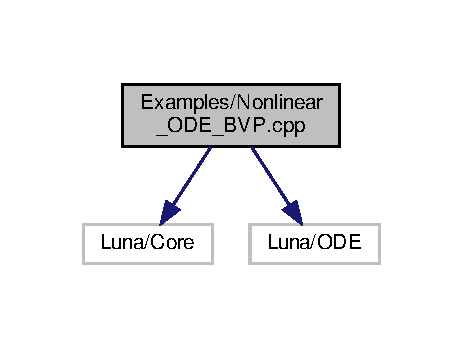
\includegraphics[width=222pt]{Nonlinear__ODE__BVP_8cpp__incl}
\end{center}
\end{figure}
\subsection*{Classes}
\begin{DoxyCompactItemize}
\item 
class \hyperlink{classLuna_1_1nonlinear__equation}{Luna\+::nonlinear\+\_\+equation}
\item 
class \hyperlink{classLuna_1_1left__BC}{Luna\+::left\+\_\+\+BC}
\item 
class \hyperlink{classLuna_1_1right__BC}{Luna\+::right\+\_\+\+BC}
\end{DoxyCompactItemize}
\subsection*{Namespaces}
\begin{DoxyCompactItemize}
\item 
 \hyperlink{namespaceLuna}{Luna}
\end{DoxyCompactItemize}
\subsection*{Enumerations}
\begin{DoxyCompactItemize}
\item 
enum \{ \hyperlink{Nonlinear__ODE__BVP_8cpp_a06fc87d81c62e9abb8790b6e5713c55ba7ce756344023b99e5ab27b804feb765c}{f}, 
\hyperlink{Nonlinear__ODE__BVP_8cpp_a06fc87d81c62e9abb8790b6e5713c55ba1e4d60e5b05464d07a30096747025a42}{fd}
 \}
\end{DoxyCompactItemize}
\subsection*{Functions}
\begin{DoxyCompactItemize}
\item 
int \hyperlink{Nonlinear__ODE__BVP_8cpp_ae66f6b31b5ad750f1fe042a706a4e3d4}{main} ()
\end{DoxyCompactItemize}


\subsection{Detailed Description}
The equation \[ (f(x)-1)f''(x) + \left( \frac{2}{x^2} - 1 \right)f'(x)^2 = 1 \] is solved subject to the boundary conditions $ f(0) = 2 $ and $ f \left(\frac{\sqrt{3}}{2} \right) = \frac{3}{2}. $ The system is solved as a set of first-\/order equations in the form \[ \begin{pmatrix} 1 & 0 \\ 0 & f(x) - 1 \end{pmatrix} \begin{bmatrix} f(x) \\ f'(x) \end{bmatrix}' = \begin{bmatrix} f'(x) \\ 1 + \left(1 - \frac{2}{x^2} \right)f'(x)^2 \end{bmatrix}, \] The exact solution is given by $ f(x) = 1 + \sqrt{1-x^2}. $. 



\subsection{Enumeration Type Documentation}
\mbox{\Hypertarget{Nonlinear__ODE__BVP_8cpp_a06fc87d81c62e9abb8790b6e5713c55b}\label{Nonlinear__ODE__BVP_8cpp_a06fc87d81c62e9abb8790b6e5713c55b}} 
\subsubsection{\texorpdfstring{anonymous enum}{anonymous enum}}
{\footnotesize\ttfamily anonymous enum}

\begin{DoxyEnumFields}{Enumerator}
\raisebox{\heightof{T}}[0pt][0pt]{\index{f@{f}!Nonlinear\+\_\+\+O\+D\+E\+\_\+\+B\+V\+P.\+cpp@{Nonlinear\+\_\+\+O\+D\+E\+\_\+\+B\+V\+P.\+cpp}}\index{Nonlinear\+\_\+\+O\+D\+E\+\_\+\+B\+V\+P.\+cpp@{Nonlinear\+\_\+\+O\+D\+E\+\_\+\+B\+V\+P.\+cpp}!f@{f}}}\mbox{\Hypertarget{Nonlinear__ODE__BVP_8cpp_a06fc87d81c62e9abb8790b6e5713c55ba7ce756344023b99e5ab27b804feb765c}\label{Nonlinear__ODE__BVP_8cpp_a06fc87d81c62e9abb8790b6e5713c55ba7ce756344023b99e5ab27b804feb765c}} 
f&\\
\hline

\raisebox{\heightof{T}}[0pt][0pt]{\index{fd@{fd}!Nonlinear\+\_\+\+O\+D\+E\+\_\+\+B\+V\+P.\+cpp@{Nonlinear\+\_\+\+O\+D\+E\+\_\+\+B\+V\+P.\+cpp}}\index{Nonlinear\+\_\+\+O\+D\+E\+\_\+\+B\+V\+P.\+cpp@{Nonlinear\+\_\+\+O\+D\+E\+\_\+\+B\+V\+P.\+cpp}!fd@{fd}}}\mbox{\Hypertarget{Nonlinear__ODE__BVP_8cpp_a06fc87d81c62e9abb8790b6e5713c55ba1e4d60e5b05464d07a30096747025a42}\label{Nonlinear__ODE__BVP_8cpp_a06fc87d81c62e9abb8790b6e5713c55ba1e4d60e5b05464d07a30096747025a42}} 
fd&\\
\hline

\end{DoxyEnumFields}


Definition at line 16 of file Nonlinear\+\_\+\+O\+D\+E\+\_\+\+B\+V\+P.\+cpp.


\begin{DoxyCode}
16 \{ \hyperlink{Nonlinear__ODE__BVP_8cpp_a06fc87d81c62e9abb8790b6e5713c55ba7ce756344023b99e5ab27b804feb765c}{f}, \hyperlink{Nonlinear__ODE__BVP_8cpp_a06fc87d81c62e9abb8790b6e5713c55ba1e4d60e5b05464d07a30096747025a42}{fd} \};
\end{DoxyCode}


\subsection{Function Documentation}
\mbox{\Hypertarget{Nonlinear__ODE__BVP_8cpp_ae66f6b31b5ad750f1fe042a706a4e3d4}\label{Nonlinear__ODE__BVP_8cpp_ae66f6b31b5ad750f1fe042a706a4e3d4}} 
\index{Nonlinear\+\_\+\+O\+D\+E\+\_\+\+B\+V\+P.\+cpp@{Nonlinear\+\_\+\+O\+D\+E\+\_\+\+B\+V\+P.\+cpp}!main@{main}}
\index{main@{main}!Nonlinear\+\_\+\+O\+D\+E\+\_\+\+B\+V\+P.\+cpp@{Nonlinear\+\_\+\+O\+D\+E\+\_\+\+B\+V\+P.\+cpp}}
\subsubsection{\texorpdfstring{main()}{main()}}
{\footnotesize\ttfamily int main (\begin{DoxyParamCaption}{ }\end{DoxyParamCaption})}



Definition at line 71 of file Nonlinear\+\_\+\+O\+D\+E\+\_\+\+B\+V\+P.\+cpp.



References f, fd, Luna\+::\+Vector$<$ T $>$\+::linspace(), Luna\+::\+O\+D\+E\+\_\+\+B\+V\+P$<$ T, X $>$\+::max\+\_\+iterations(), Heat\+\_\+plot\+::N, Luna\+::\+Mesh1\+D$<$ T, X $>$\+::output(), Luna\+::\+O\+D\+E\+\_\+\+B\+V\+P$<$ T, X $>$\+::set\+\_\+monitor\+\_\+det(), Luna\+::\+Vector$<$ T $>$\+::size(), Luna\+::\+O\+D\+E\+\_\+\+B\+V\+P$<$ T, X $>$\+::solution(), Luna\+::\+O\+D\+E\+\_\+\+B\+V\+P$<$ T, X $>$\+::solve\+\_\+bvp(), Luna\+::\+O\+D\+E\+\_\+\+B\+V\+P$<$ T, X $>$\+::tolerance(), and Heat\+\_\+plot\+::x.


\begin{DoxyCode}
72 \{
73   cout << \textcolor{stringliteral}{"------------------- Nonlinear\_ODE\_BVP ------------------"} << endl;
74   \textcolor{comment}{// Setup the domain}
75   \textcolor{keywordtype}{double} left( 0.0 );                \textcolor{comment}{// Left boundary}
76   \textcolor{keywordtype}{double} right( sqrt(3.0) / 2.0 );   \textcolor{comment}{// Right boundary}
77     std::size\_t \hyperlink{namespaceHeat__plot_a7d050092798e28458a263710837bda77}{N}( 50 );               \textcolor{comment}{// Number of nodes}
78     \hyperlink{classLuna_1_1Vector}{Vector<double>} nodes;                        \textcolor{comment}{// Vector of nodes ( uniformly spaced )}
79     nodes.\hyperlink{classLuna_1_1Vector_a275847fc0bddea86c66651201a6db82e}{linspace}( left, right, \hyperlink{namespaceHeat__plot_a7d050092798e28458a263710837bda77}{N});
80 
81   cout << \textcolor{stringliteral}{" * The nonlinear boundary problem is solved on a uniform"} << endl
82        << \textcolor{stringliteral}{" * grid in the domain "} << left << \textcolor{stringliteral}{" < x < "} << right
83        << \textcolor{stringliteral}{" containing N = "} << \hyperlink{namespaceHeat__plot_a7d050092798e28458a263710837bda77}{N} << endl << \textcolor{stringliteral}{" * nodal points."} << endl;
84 
85   \textcolor{comment}{// Create instances of the equation and BCs}
86   \hyperlink{classLuna_1_1nonlinear__equation}{nonlinear\_equation} equation;
87   \hyperlink{classLuna_1_1left__BC}{left\_BC} left\_bc;
88   \hyperlink{classLuna_1_1right__BC}{right\_BC} right\_bc;
89 
90   \textcolor{comment}{// Create boundary value problem}
91   \hyperlink{classLuna_1_1ODE__BVP}{ODE\_BVP<double>} ode( &equation, nodes, &left\_bc, &right\_bc );
92 
93   \textcolor{comment}{/* ----- Set the initial guess ----- */}
94   \textcolor{comment}{// f = 2 - (1/sqrt(3))x (linear fit to boundary conditions)}
95   \textcolor{keywordtype}{double} gradient( - 1.0 / sqrt(3) );
96     \textcolor{keywordflow}{for} (std::size\_t j=0; j < \hyperlink{namespaceHeat__plot_a7d050092798e28458a263710837bda77}{N}; ++j )
97     \{
98         \textcolor{keywordtype}{double} \hyperlink{namespaceHeat__plot_aa88370c16b85b784ccbde3ed88bc1991}{x} = nodes[ j ];
99         ode.solution()( j, \hyperlink{Nonlinear__ODE__BVP_8cpp_a06fc87d81c62e9abb8790b6e5713c55ba7ce756344023b99e5ab27b804feb765c}{f} )  = 2.0 + gradient * x;
100     ode.solution()( j, \hyperlink{Nonlinear__ODE__BVP_8cpp_a06fc87d81c62e9abb8790b6e5713c55ba1e4d60e5b05464d07a30096747025a42}{fd} ) = gradient;
101     \}
102 
103   ode.tolerance() = 1e-8;
104   ode.max\_iterations() = 50;
105   ode.set\_monitor\_det( \textcolor{keyword}{false} );
106 
107   \textcolor{comment}{// Solve}
108   ode.solve\_bvp();
109 
110   nodes = ode.solution().nodes();
111   \hyperlink{classLuna_1_1Mesh1D}{Mesh1D<double, double>} exact\_solution( nodes, 2 );
112   \textcolor{keywordflow}{for} (std::size\_t j=0; j < nodes.\hyperlink{classLuna_1_1Vector_ac9b6ed7a0df401728f27c193fbc8f4d8}{size}(); ++j )
113     \{
114         \textcolor{keywordtype}{double} x = nodes[ j ];
115         exact\_solution( j, \hyperlink{Nonlinear__ODE__BVP_8cpp_a06fc87d81c62e9abb8790b6e5713c55ba7ce756344023b99e5ab27b804feb765c}{f} )  = 1.0 + sqrt( 1.0 - x * x );
116     exact\_solution( j, \hyperlink{Nonlinear__ODE__BVP_8cpp_a06fc87d81c62e9abb8790b6e5713c55ba1e4d60e5b05464d07a30096747025a42}{fd} ) = - x / sqrt( 1.0 - x * x );
117     \}
118 
119   \textcolor{comment}{// Output the solution data}
120   ode.solution().output( \textcolor{stringliteral}{"./DATA/ODE\_BVP\_numerical\_solution.dat"} );
121   exact\_solution.output( \textcolor{stringliteral}{"./DATA/ODE\_BVP\_exact\_solution.dat"} );
122 
123   cout << \textcolor{stringliteral}{" * To plot the numerical solution, the exact solution "} << endl
124        << \textcolor{stringliteral}{" * and the error between the two run:"} << endl
125        << \textcolor{stringliteral}{"python Plotting/Nonlinear\_ODE\_BVP\_plot.py"} << endl;
126   cout << \textcolor{stringliteral}{"--- FINISHED ---"} << endl;
127 \}
\end{DoxyCode}

\hypertarget{ODE__BVP__test_8cpp}{}\section{Examples/\+O\+D\+E\+\_\+\+B\+V\+P\+\_\+test.cpp File Reference}
\label{ODE__BVP__test_8cpp}\index{Examples/\+O\+D\+E\+\_\+\+B\+V\+P\+\_\+test.\+cpp@{Examples/\+O\+D\+E\+\_\+\+B\+V\+P\+\_\+test.\+cpp}}


T\+O\+DO description / rename file.  


{\ttfamily \#include \char`\"{}Luna/\+Core\char`\"{}}\newline
{\ttfamily \#include \char`\"{}Luna/\+O\+DE\char`\"{}}\newline
Include dependency graph for O\+D\+E\+\_\+\+B\+V\+P\+\_\+test.\+cpp\+:\nopagebreak
\begin{figure}[H]
\begin{center}
\leavevmode
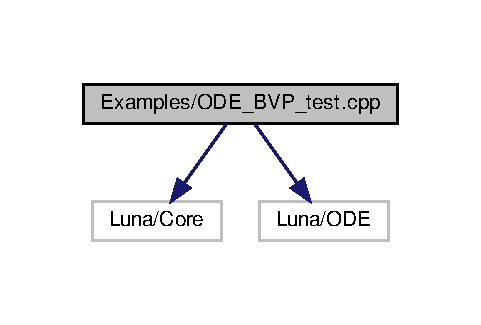
\includegraphics[width=231pt]{ODE__BVP__test_8cpp__incl}
\end{center}
\end{figure}
\subsection*{Classes}
\begin{DoxyCompactItemize}
\item 
class \hyperlink{classLuna_1_1test__equation}{Luna\+::test\+\_\+equation}
\item 
class \hyperlink{classLuna_1_1left__BC}{Luna\+::left\+\_\+\+BC}
\item 
class \hyperlink{classLuna_1_1right__BC}{Luna\+::right\+\_\+\+BC}
\end{DoxyCompactItemize}
\subsection*{Namespaces}
\begin{DoxyCompactItemize}
\item 
 \hyperlink{namespaceLuna}{Luna}
\end{DoxyCompactItemize}
\subsection*{Enumerations}
\begin{DoxyCompactItemize}
\item 
enum \{ \hyperlink{ODE__BVP__test_8cpp_adf764cbdea00d65edcd07bb9953ad2b7ae1f9fdb8b786c63efc4ce44eeacd17f2}{y}, 
\hyperlink{ODE__BVP__test_8cpp_adf764cbdea00d65edcd07bb9953ad2b7ae006cbf64cf3ff4ee152bf490ae2e2a7}{yd}
 \}
\end{DoxyCompactItemize}
\subsection*{Functions}
\begin{DoxyCompactItemize}
\item 
int \hyperlink{ODE__BVP__test_8cpp_ae66f6b31b5ad750f1fe042a706a4e3d4}{main} ()
\end{DoxyCompactItemize}


\subsection{Detailed Description}
T\+O\+DO description / rename file. 



\subsection{Enumeration Type Documentation}
\mbox{\Hypertarget{ODE__BVP__test_8cpp_adf764cbdea00d65edcd07bb9953ad2b7}\label{ODE__BVP__test_8cpp_adf764cbdea00d65edcd07bb9953ad2b7}} 
\subsubsection{\texorpdfstring{anonymous enum}{anonymous enum}}
{\footnotesize\ttfamily anonymous enum}

\begin{DoxyEnumFields}{Enumerator}
\raisebox{\heightof{T}}[0pt][0pt]{\index{y@{y}!O\+D\+E\+\_\+\+B\+V\+P\+\_\+test.\+cpp@{O\+D\+E\+\_\+\+B\+V\+P\+\_\+test.\+cpp}}\index{O\+D\+E\+\_\+\+B\+V\+P\+\_\+test.\+cpp@{O\+D\+E\+\_\+\+B\+V\+P\+\_\+test.\+cpp}!y@{y}}}\mbox{\Hypertarget{ODE__BVP__test_8cpp_adf764cbdea00d65edcd07bb9953ad2b7ae1f9fdb8b786c63efc4ce44eeacd17f2}\label{ODE__BVP__test_8cpp_adf764cbdea00d65edcd07bb9953ad2b7ae1f9fdb8b786c63efc4ce44eeacd17f2}} 
y&\\
\hline

\raisebox{\heightof{T}}[0pt][0pt]{\index{yd@{yd}!O\+D\+E\+\_\+\+B\+V\+P\+\_\+test.\+cpp@{O\+D\+E\+\_\+\+B\+V\+P\+\_\+test.\+cpp}}\index{O\+D\+E\+\_\+\+B\+V\+P\+\_\+test.\+cpp@{O\+D\+E\+\_\+\+B\+V\+P\+\_\+test.\+cpp}!yd@{yd}}}\mbox{\Hypertarget{ODE__BVP__test_8cpp_adf764cbdea00d65edcd07bb9953ad2b7ae006cbf64cf3ff4ee152bf490ae2e2a7}\label{ODE__BVP__test_8cpp_adf764cbdea00d65edcd07bb9953ad2b7ae006cbf64cf3ff4ee152bf490ae2e2a7}} 
yd&\\
\hline

\end{DoxyEnumFields}


Definition at line 9 of file O\+D\+E\+\_\+\+B\+V\+P\+\_\+test.\+cpp.


\begin{DoxyCode}
9 \{ \hyperlink{ODE__BVP__test_8cpp_adf764cbdea00d65edcd07bb9953ad2b7ae1f9fdb8b786c63efc4ce44eeacd17f2}{y}, \hyperlink{ODE__BVP__test_8cpp_adf764cbdea00d65edcd07bb9953ad2b7ae006cbf64cf3ff4ee152bf490ae2e2a7}{yd} \};
\end{DoxyCode}


\subsection{Function Documentation}
\mbox{\Hypertarget{ODE__BVP__test_8cpp_ae66f6b31b5ad750f1fe042a706a4e3d4}\label{ODE__BVP__test_8cpp_ae66f6b31b5ad750f1fe042a706a4e3d4}} 
\index{O\+D\+E\+\_\+\+B\+V\+P\+\_\+test.\+cpp@{O\+D\+E\+\_\+\+B\+V\+P\+\_\+test.\+cpp}!main@{main}}
\index{main@{main}!O\+D\+E\+\_\+\+B\+V\+P\+\_\+test.\+cpp@{O\+D\+E\+\_\+\+B\+V\+P\+\_\+test.\+cpp}}
\subsubsection{\texorpdfstring{main()}{main()}}
{\footnotesize\ttfamily int main (\begin{DoxyParamCaption}{ }\end{DoxyParamCaption})}



Definition at line 63 of file O\+D\+E\+\_\+\+B\+V\+P\+\_\+test.\+cpp.



References Luna\+::\+Vector$<$ T $>$\+::linspace(), Luna\+::\+O\+D\+E\+\_\+\+B\+V\+P$<$ T, X $>$\+::max\+\_\+iterations(), Heat\+\_\+plot\+::N, Luna\+::\+Mesh1\+D$<$ T, X $>$\+::output(), Luna\+::\+O\+D\+E\+\_\+\+B\+V\+P$<$ T, X $>$\+::set\+\_\+monitor\+\_\+det(), Luna\+::\+Vector$<$ T $>$\+::size(), Luna\+::\+O\+D\+E\+\_\+\+B\+V\+P$<$ T, X $>$\+::solution(), Luna\+::\+O\+D\+E\+\_\+\+B\+V\+P$<$ T, X $>$\+::solve\+\_\+bvp(), Luna\+::\+O\+D\+E\+\_\+\+B\+V\+P$<$ T, X $>$\+::tolerance(), Heat\+\_\+plot\+::x, y, and yd.


\begin{DoxyCode}
64 \{
65   cout << \textcolor{stringliteral}{"--------------------- ODE\_BVP --------------------"} << endl;
66 
67   \textcolor{comment}{// Setup the domain}
68 
69   \textcolor{keywordtype}{double} left( 0.0 );               \textcolor{comment}{// Left boundary}
70   \textcolor{keywordtype}{double} right( M\_PI / 4.0 );             \textcolor{comment}{// Right boundary}
71     std::size\_t \hyperlink{namespaceHeat__plot_a7d050092798e28458a263710837bda77}{N}( 1000 );            \textcolor{comment}{// Number of nodes}
72     \hyperlink{classLuna_1_1Vector}{Vector<double>} nodes;                       \textcolor{comment}{// Vector of nodes ( uniformly spaced )}
73     nodes.\hyperlink{classLuna_1_1Vector_a275847fc0bddea86c66651201a6db82e}{linspace}( left, right, \hyperlink{namespaceHeat__plot_a7d050092798e28458a263710837bda77}{N});
74 
75   \textcolor{comment}{// Create instances of the equation and BCs}
76   \hyperlink{classLuna_1_1test__equation}{test\_equation} equation;
77   \hyperlink{classLuna_1_1left__BC}{left\_BC} left\_bc;
78   \hyperlink{classLuna_1_1right__BC}{right\_BC} right\_bc;
79 
80   \textcolor{comment}{// Create boundary value problem}
81   \hyperlink{classLuna_1_1ODE__BVP}{ODE\_BVP<double>} ode( &equation, nodes, &left\_bc, &right\_bc );
82 
83   \textcolor{comment}{/* ----- Set the initial guess ----- */}
84   \textcolor{comment}{// y = (48/pi)x - 2 (linear fit to boundary conditions)}
85   \textcolor{keywordtype}{double} gradient( 48.0 / M\_PI );
86     \textcolor{keywordflow}{for} (std::size\_t j=0; j < \hyperlink{namespaceHeat__plot_a7d050092798e28458a263710837bda77}{N}; ++j )
87     \{
88         \textcolor{keywordtype}{double} \hyperlink{namespaceHeat__plot_aa88370c16b85b784ccbde3ed88bc1991}{x} = nodes[ j ];
89         ode.solution()( j, \hyperlink{ODE__BVP__test_8cpp_adf764cbdea00d65edcd07bb9953ad2b7ae1f9fdb8b786c63efc4ce44eeacd17f2}{y} )  = gradient * x - 2.0;
90     ode.solution()( j, \hyperlink{ODE__BVP__test_8cpp_adf764cbdea00d65edcd07bb9953ad2b7ae006cbf64cf3ff4ee152bf490ae2e2a7}{yd} ) = gradient;
91     \}
92 
93   ode.tolerance() = 1e-8;
94   ode.max\_iterations() = 50;
95   ode.set\_monitor\_det( \textcolor{keyword}{false} );
96 
97   \textcolor{comment}{// Adaptively solve the BVP}
98   \textcolor{comment}{//ode.adapt\_until( 1e-7 );}
99 
100   cout << \textcolor{stringliteral}{" Number of nodes in the solution = "} << ode.solution().nnodes()
101        << endl;
102 
103   nodes = ode.solution().nodes();
104   \hyperlink{classLuna_1_1Mesh1D}{Mesh1D<double, double>} exact\_solution( nodes, 2 );
105   \textcolor{keywordflow}{for} (std::size\_t j=0; j < nodes.\hyperlink{classLuna_1_1Vector_ac9b6ed7a0df401728f27c193fbc8f4d8}{size}(); ++j )
106     \{
107         \textcolor{keywordtype}{double} x = nodes[ j ];
108         exact\_solution( j, \hyperlink{ODE__BVP__test_8cpp_adf764cbdea00d65edcd07bb9953ad2b7ae1f9fdb8b786c63efc4ce44eeacd17f2}{y} )  = - 2.0 * cos( 2 * x ) + 10.0 * sin( 2 * x );
109     exact\_solution( j, \hyperlink{ODE__BVP__test_8cpp_adf764cbdea00d65edcd07bb9953ad2b7ae006cbf64cf3ff4ee152bf490ae2e2a7}{yd} ) =   4.0 * sin( 2 * x ) + 20.0 * cos( 2 * x );
110     \}
111   \textcolor{comment}{// Solve}
112   ode.solve\_bvp();
113 
114   \textcolor{comment}{// Output the solution data}
115   ode.solution().output( \textcolor{stringliteral}{"./DATA/ODE\_BVP\_numerical\_solution.dat"} );
116   exact\_solution.output( \textcolor{stringliteral}{"./DATA/ODE\_BVP\_exact\_solution.dat"} );
117 
118   \textcolor{comment}{//TODO plotting instructions}
119 
120   cout << \textcolor{stringliteral}{"--- FINISHED ---"} << endl;
121 \}
\end{DoxyCode}

\hypertarget{Root__finding_8cpp}{}\section{Examples/\+Root\+\_\+finding.cpp File Reference}
\label{Root__finding_8cpp}\index{Examples/\+Root\+\_\+finding.\+cpp@{Examples/\+Root\+\_\+finding.\+cpp}}


Examples of the numerical solution of equations using Newton\textquotesingle{}s method and arc-\/length continuation and the solution of polynomial equations.  


{\ttfamily \#include \char`\"{}Luna/\+Core\char`\"{}}\newline
Include dependency graph for Root\+\_\+finding.\+cpp\+:\nopagebreak
\begin{figure}[H]
\begin{center}
\leavevmode
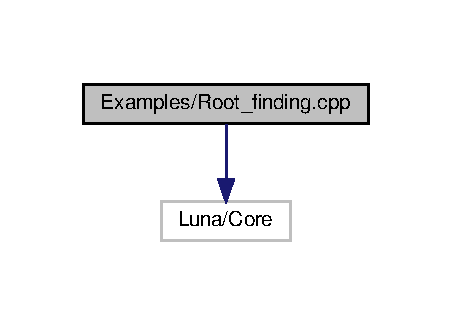
\includegraphics[width=217pt]{Root__finding_8cpp__incl}
\end{center}
\end{figure}
\subsection*{Classes}
\begin{DoxyCompactItemize}
\item 
class \hyperlink{classLuna_1_1test__residual}{Luna\+::test\+\_\+residual}
\item 
class \hyperlink{classLuna_1_1Arc__problem}{Luna\+::\+Arc\+\_\+problem}
\end{DoxyCompactItemize}
\subsection*{Namespaces}
\begin{DoxyCompactItemize}
\item 
 \hyperlink{namespaceLuna}{Luna}
\end{DoxyCompactItemize}
\subsection*{Functions}
\begin{DoxyCompactItemize}
\item 
int \hyperlink{Root__finding_8cpp_ae66f6b31b5ad750f1fe042a706a4e3d4}{main} ()
\end{DoxyCompactItemize}


\subsection{Detailed Description}
Examples of the numerical solution of equations using Newton\textquotesingle{}s method and arc-\/length continuation and the solution of polynomial equations. 



\subsection{Function Documentation}
\mbox{\Hypertarget{Root__finding_8cpp_ae66f6b31b5ad750f1fe042a706a4e3d4}\label{Root__finding_8cpp_ae66f6b31b5ad750f1fe042a706a4e3d4}} 
\index{Root\+\_\+finding.\+cpp@{Root\+\_\+finding.\+cpp}!main@{main}}
\index{main@{main}!Root\+\_\+finding.\+cpp@{Root\+\_\+finding.\+cpp}}
\subsubsection{\texorpdfstring{main()}{main()}}
{\footnotesize\ttfamily int main (\begin{DoxyParamCaption}{ }\end{DoxyParamCaption})}



Definition at line 51 of file Root\+\_\+finding.\+cpp.



References Luna\+::\+Newton$<$ T $>$\+::arclength\+\_\+solve(), Luna\+::\+Polynomial$<$ T $>$\+::coeffs(), f, Luna\+::\+Arclength$<$ T $>$\+::init\+\_\+arc(), Luna\+::\+Arc\+\_\+problem\+::p, Luna\+::\+Polynomial$<$ T $>$\+::quadratic\+\_\+solve(), Luna\+::\+Polynomial$<$ T $>$\+::roots(), Luna\+::\+Newton$<$ T $>$\+::solve(), and Heat\+\_\+plot\+::u.


\begin{DoxyCode}
52 \{
53   cout << \textcolor{stringliteral}{"----------------- Root finding -----------------"} << endl;
54 
55   cout << \textcolor{stringliteral}{" * Solving the set of equations "} << endl
56        << \textcolor{stringliteral}{" * x^3 + y - 1 = 0, "} << endl
57        << \textcolor{stringliteral}{" * y^3 - x + 1 = 0, "} << endl
58        << \textcolor{stringliteral}{" * using Newton's method and the initial guess "} << endl;
59 
60   \hyperlink{classLuna_1_1test__residual}{Luna::test\_residual} Res;                           \textcolor{comment}{// Create residual}
61   \hyperlink{classLuna_1_1Vector}{Vector<double>} x\_0(2, 0.5);                        \textcolor{comment}{// Initial guess}
62   x\_0[1] = 0.25;
63   cout << \textcolor{stringliteral}{" * x\_0 = "} << x\_0 << endl;
64   \hyperlink{classLuna_1_1Newton}{Luna::Newton<double>} newton( &Res );               \textcolor{comment}{// Create Newton object}
65   newton.solve( x\_0 );                               \textcolor{comment}{// Solve the system}
66 
67   cout << \textcolor{stringliteral}{" * gives the solution (x,y)= "} << x\_0 << endl;
68 
69   cout << endl << \textcolor{stringliteral}{"----- Arc continuation of x^2 + p^2 = 2.0 -----"} << endl;
70 
71   \textcolor{comment}{// Instantiate the problem}
72   \hyperlink{classLuna_1_1Arc__problem}{Luna::Arc\_problem} arc\_prob;
73   arc\_prob.\hyperlink{classLuna_1_1Arc__problem_ab747ff77d23c83ebf8e0e8ab58e9c432}{p} = 1.0;
74 
75   \textcolor{keyword}{const} \textcolor{keywordtype}{double} tol = 1.e-6;
76   \textcolor{comment}{// Scalar newton iteration problem}
77   \hyperlink{classLuna_1_1Newton}{Luna::Newton<double>} newton\_arc( &arc\_prob, 8, tol );
78 
79   \textcolor{comment}{// Initial guess}
80   \hyperlink{classLuna_1_1Vector}{Vector<double>} state( 1, 1.0 );
81   \textcolor{keywordtype}{double} arc\_step( 0.1 );
82   \textcolor{keywordtype}{double} max\_arc\_step( 0.5 );
83   newton\_arc.init\_arc( state, &arc\_prob.\hyperlink{classLuna_1_1Arc__problem_ab747ff77d23c83ebf8e0e8ab58e9c432}{p}, arc\_step, max\_arc\_step );
84 
85   \textcolor{keywordflow}{do}
86   \{
87     newton\_arc.arclength\_solve( state );
88     cout << \textcolor{stringliteral}{"x = "} << state[ 0 ] << \textcolor{stringliteral}{", p = "} << arc\_prob.\hyperlink{classLuna_1_1Arc__problem_ab747ff77d23c83ebf8e0e8ab58e9c432}{p} << endl;
89   \}\textcolor{keywordflow}{while}( state[ 0 ] < 1.0 );
90 
91   cout << endl << \textcolor{stringliteral}{"--------- Polynomial equations ---------"} << endl;
92   cout << \textcolor{stringliteral}{" * Define the function f(x) = -1 + 2x + x^2"} << endl;
93   \hyperlink{classLuna_1_1Polynomial}{Luna::Polynomial<double>} \hyperlink{Nonlinear__ODE__BVP_8cpp_a06fc87d81c62e9abb8790b6e5713c55ba7ce756344023b99e5ab27b804feb765c}{f}( std::vector<double> \{ -1.0, 2.0, 1.0, 1.0 \} );
94   cout << \textcolor{stringliteral}{" * Access the x coefficient f[1] = "} << \hyperlink{Nonlinear__ODE__BVP_8cpp_a06fc87d81c62e9abb8790b6e5713c55ba7ce756344023b99e5ab27b804feb765c}{f}[1] << endl;
95   cout << \textcolor{stringliteral}{" * Evaluate the polynomial at x = 0.1 "} << endl
96        << \textcolor{stringliteral}{" * f( 0.1 ) = "} << \hyperlink{Nonlinear__ODE__BVP_8cpp_a06fc87d81c62e9abb8790b6e5713c55ba7ce756344023b99e5ab27b804feb765c}{f}( 0.1 ) << endl << endl;
97 
98   cout << \textcolor{stringliteral}{" * Solve the complex quadratic equation "} << endl
99        << \textcolor{stringliteral}{" * ( 1 + i )x^2 - ( 2 + i )x - 1 = 0 "} << endl;
100   \hyperlink{classLuna_1_1Polynomial}{Luna::Polynomial< std::complex<double>} > p;
101   std::complex<double> a ( 1.0, 1.0 );
102   std::complex<double> b ( - 2.0, - 1.0 );
103   std::complex<double> c ( - 1.0, 0.0 );
104   \hyperlink{classLuna_1_1Vector}{Vector< std::complex<double>} > roots;
105   roots = p.\hyperlink{classLuna_1_1Polynomial_a801a06a8f76a415ce1368daea1c77abb}{quadratic\_solve}( a, b, c );
106   cout << \textcolor{stringliteral}{" * The two roots of the equation are"} << endl;
107   cout << \textcolor{stringliteral}{" * x\_0 = "} << roots[ 0 ] << endl;
108   cout << \textcolor{stringliteral}{" * x\_1 = "} << roots[ 1 ] << endl << endl;
109 
110   cout << \textcolor{stringliteral}{" * Solve the cubic equation"} << endl
111        << \textcolor{stringliteral}{" * 2x^3 + x^2 + 2x - 1 = 0 "} << endl;
112   \hyperlink{classLuna_1_1Vector}{Vector<std::complex<double>}> f\_roots;
113   f\_roots = \hyperlink{Nonlinear__ODE__BVP_8cpp_a06fc87d81c62e9abb8790b6e5713c55ba7ce756344023b99e5ab27b804feb765c}{f}.cubic\_solve( 2.0, 1.0, 2.0, - 1.0 );
114   cout << \textcolor{stringliteral}{" * The three roots of the equation are"} << endl;
115   cout << \textcolor{stringliteral}{" * x\_0 = "} << f\_roots[ 0 ] << endl;
116   cout << \textcolor{stringliteral}{" * x\_1 = "} << f\_roots[ 1 ] << endl;
117   cout << \textcolor{stringliteral}{" * x\_2 = "} << f\_roots[ 2 ] << endl << endl;
118 
119   cout << \textcolor{stringliteral}{" * Dividing the polynomial u(x) = x^3 - 2x^2 - 4"} << endl
120        << \textcolor{stringliteral}{" * by v(x) = x - 3 gives the quotient "} << endl;
121   \hyperlink{classLuna_1_1Polynomial}{Polynomial<double>} \hyperlink{namespaceHeat__plot_ae622b86afa46daa3e9b887624ab1bf26}{u}( std::vector<double> \{ -4.0, 0.0, -2.0, 1.0 \} );
122   \hyperlink{classLuna_1_1Polynomial}{Polynomial<double>} v( std::vector<double> \{ -3.0, 1.0 \} );
123   \hyperlink{classLuna_1_1Polynomial}{Polynomial<double>} q, r;
124   \hyperlink{namespaceHeat__plot_ae622b86afa46daa3e9b887624ab1bf26}{u}.polydiv( v, q, r );
125   cout << \textcolor{stringliteral}{" * q(x) = "} << q.\hyperlink{classLuna_1_1Polynomial_ab5e966c308b7e66d9c1c20666926db34}{coeffs}()[0] << \textcolor{stringliteral}{" + "} << q.\hyperlink{classLuna_1_1Polynomial_ab5e966c308b7e66d9c1c20666926db34}{coeffs}()[1] << \textcolor{stringliteral}{"x + "}
126        << q.\hyperlink{classLuna_1_1Polynomial_ab5e966c308b7e66d9c1c20666926db34}{coeffs}()[2] << \textcolor{stringliteral}{"x^2"} << endl
127        << \textcolor{stringliteral}{" * and the remainder "} << endl
128        << \textcolor{stringliteral}{" * r(x) = "} << r.\hyperlink{classLuna_1_1Polynomial_ab5e966c308b7e66d9c1c20666926db34}{coeffs}() << endl
129        << \textcolor{stringliteral}{" * such that u(x) = q(x) * v(x) + r(x)."} << endl << endl;
130 
131   cout << \textcolor{stringliteral}{" * Find the roots of the quartic equation "} << endl
132        << \textcolor{stringliteral}{" * 3 + x + x^2 + x^4 = 0 using Laguerre's method. "} << endl;
133   \hyperlink{classLuna_1_1Polynomial}{Polynomial<double>} poly( std::vector<double> \{ 3.0, 1.0, 1.0, 0.0, 1.0 \} );
134   \hyperlink{classLuna_1_1Vector}{Vector<std::complex<double>}> poly\_roots;
135   poly\_roots = poly.\hyperlink{classLuna_1_1Polynomial_ab045b5ac29660de6d5a54246ed1bec70}{roots}( \textcolor{keyword}{true} );
136   cout << \textcolor{stringliteral}{" * The roots of the equation are"} << endl
137        << \textcolor{stringliteral}{" * x\_0 = "} << poly\_roots[0] << endl
138        << \textcolor{stringliteral}{" * x\_1 = "} << poly\_roots[1] << endl
139        << \textcolor{stringliteral}{" * x\_2 = "} << poly\_roots[2] << endl
140        << \textcolor{stringliteral}{" * x\_3 = "} << poly\_roots[3] << endl << endl;
141 
142   cout << \textcolor{stringliteral}{"--- FINISHED ---"} << endl;
143 \}
\end{DoxyCode}

\hypertarget{Sparse__test_8cpp}{}\section{Examples/\+Sparse\+\_\+test.cpp File Reference}
\label{Sparse__test_8cpp}\index{Examples/\+Sparse\+\_\+test.\+cpp@{Examples/\+Sparse\+\_\+test.\+cpp}}


T\+O\+DO description / rename file.  


{\ttfamily \#include \char`\"{}Luna/\+Core\char`\"{}}\newline
{\ttfamily \#include \char`\"{}Luna/\+Sparse\char`\"{}}\newline
Include dependency graph for Sparse\+\_\+test.\+cpp\+:\nopagebreak
\begin{figure}[H]
\begin{center}
\leavevmode
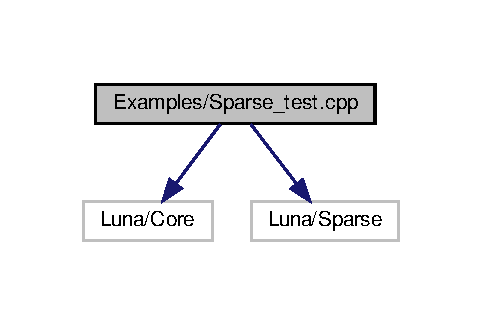
\includegraphics[width=232pt]{Sparse__test_8cpp__incl}
\end{center}
\end{figure}
\subsection*{Functions}
\begin{DoxyCompactItemize}
\item 
int \hyperlink{Sparse__test_8cpp_ae66f6b31b5ad750f1fe042a706a4e3d4}{main} ()
\end{DoxyCompactItemize}


\subsection{Detailed Description}
T\+O\+DO description / rename file. 



\subsection{Function Documentation}
\mbox{\Hypertarget{Sparse__test_8cpp_ae66f6b31b5ad750f1fe042a706a4e3d4}\label{Sparse__test_8cpp_ae66f6b31b5ad750f1fe042a706a4e3d4}} 
\index{Sparse\+\_\+test.\+cpp@{Sparse\+\_\+test.\+cpp}!main@{main}}
\index{main@{main}!Sparse\+\_\+test.\+cpp@{Sparse\+\_\+test.\+cpp}}
\subsubsection{\texorpdfstring{main()}{main()}}
{\footnotesize\ttfamily int main (\begin{DoxyParamCaption}{ }\end{DoxyParamCaption})}



Definition at line 11 of file Sparse\+\_\+test.\+cpp.



References Luna\+::\+Sparse\+Matrix$<$ T $>$\+::col\+\_\+start(), Luna\+::\+Vector$<$ T $>$\+::insert(), Luna\+::\+Sparse\+Matrix$<$ T $>$\+::multiply(), Luna\+::\+Sparse\+Matrix$<$ T $>$\+::nonzero(), Luna\+::\+Vector$<$ T $>$\+::random(), Luna\+::\+Sparse\+Matrix$<$ T $>$\+::row\+\_\+index(), Luna\+::\+Sparse\+Matrix$<$ T $>$\+::solve\+\_\+\+Bi\+C\+G(), Luna\+::\+Sparse\+Matrix$<$ T $>$\+::solve\+\_\+\+Bi\+C\+G\+S\+T\+A\+B(), Luna\+::\+Sparse\+Matrix$<$ T $>$\+::val(), Heat\+\_\+plot\+::x, and y.


\begin{DoxyCode}
12 \{
13   cout << \textcolor{stringliteral}{"--------------------- Sparse Matrices --------------------"} << endl;
14 
15   \hyperlink{classLuna_1_1Vector}{Vector<double>} val( \{ 3., 4., 7., 1., 5., 2., 9., 6., 5. \} );
16   \hyperlink{classLuna_1_1Vector}{Vector<std::size\_t>} row\_ind( \{ 0, 1, 2, 0, 2, 0, 2, 4, 4 \} );
17   \hyperlink{classLuna_1_1Vector}{Vector<std::size\_t>} col\_ptr( \{ 0, 1, 3, 5, 8, 9 \} );
18 
19   \hyperlink{classLuna_1_1SparseMatrix}{SparseMatrix<double>} sparse( 5, 5, val, row\_ind, col\_ptr );
20 
21 
22   cout << \textcolor{stringliteral}{" * val       = "} << sparse.val() << endl;
23   cout << \textcolor{stringliteral}{" * row\_index = "} << sparse.row\_index() << endl;
24   cout << \textcolor{stringliteral}{" * col\_start = "} << sparse.col\_start() << endl;
25   cout << \textcolor{stringliteral}{" * nonzeros  = "} << sparse.nonzero() << endl;
26 
27   sparse.insert( 1, 3, 2.0 );
28   sparse.insert( 1, 0, 5.0 );
29 
30   cout << \textcolor{stringliteral}{" * val       = "} << sparse.val() << endl;
31   cout << \textcolor{stringliteral}{" * row\_index = "} << sparse.row\_index() << endl;
32   cout << \textcolor{stringliteral}{" * col\_start = "} << sparse.col\_start() << endl;
33   cout << \textcolor{stringliteral}{" * nonzeros  = "} << sparse.nonzero() << endl;
34 
35   \textcolor{keyword}{typedef} \hyperlink{classLuna_1_1Triplet}{Triplet<double>} Td;
36   \hyperlink{classLuna_1_1Vector}{Vector<Td>} triplets \{ Td( 0, 3, 2.0 ), Td( 2, 3, 9.0 ), Td( 4, 3, 6.0 ),
37                         Td( 4, 4, 5.0 ), Td( 0, 0, 3.0 ), Td( 1, 1, 4.0 ) \};
38 
39   triplets( Td( 2, 1, 7.0 ) );
40   triplets( Td( 0, 2, 1.0 ) );
41   triplets( Td( 2, 2, 5.0 ) );
42   triplets( Td( 3, 2, 1.0 ) );
43 
44   \hyperlink{classLuna_1_1SparseMatrix}{SparseMatrix<double>} sparse\_trip( 5, 5, triplets );
45   cout << \textcolor{stringliteral}{" * val       = "} << sparse\_trip.val() << endl;
46   cout << \textcolor{stringliteral}{" * row\_index = "} << sparse\_trip.row\_index() << endl;
47   cout << \textcolor{stringliteral}{" * col\_start = "} << sparse\_trip.col\_start() << endl;
48   cout << \textcolor{stringliteral}{" * nonzeros  = "} << sparse\_trip.nonzero() << endl;
49 
50   \hyperlink{classLuna_1_1Vector}{Vector<double>} b \{ 1, 2, 3, 4, 5 \};
51   \hyperlink{classLuna_1_1Vector}{Vector<double>} \hyperlink{namespaceHeat__plot_aa88370c16b85b784ccbde3ed88bc1991}{x}( 5, 0.0 );
52 
53   \textcolor{keywordtype}{int} iter( 100 );
54   \textcolor{keywordtype}{double} tol( 1e-8 );
55   \textcolor{keywordtype}{int} code = sparse\_trip.solve\_BiCG( b, \hyperlink{namespaceHeat__plot_aa88370c16b85b784ccbde3ed88bc1991}{x}, iter, tol );
56 
57   cout << \textcolor{stringliteral}{" * x = "} << \hyperlink{namespaceHeat__plot_aa88370c16b85b784ccbde3ed88bc1991}{x} << endl;
58   cout << \textcolor{stringliteral}{" * iter = "} << iter << endl;
59   cout << \textcolor{stringliteral}{" * err = "} << scientific << tol << endl;
60 
61   \textcolor{comment}{//TODO need to test a complex sparse matrix}
62 
63   \textcolor{keyword}{typedef} std::complex<double> \hyperlink{namespaceLuna_af3257e90072a78a8ffb16a16773aa18e}{cmplx};
64   \textcolor{keyword}{typedef} \hyperlink{classLuna_1_1Triplet}{Triplet<cmplx>} Tc;
65 
66   \hyperlink{classLuna_1_1Vector}{Vector<Tc>} trips;
67 
68   trips( Tc( 0, 0, \hyperlink{namespaceLuna_af3257e90072a78a8ffb16a16773aa18e}{cmplx}( 1.0, 1.0 ) ) );
69   trips( Tc( 0, 1, \hyperlink{namespaceLuna_af3257e90072a78a8ffb16a16773aa18e}{cmplx}( -1.0, 0.0 ) ) );
70   trips( Tc( 1, 0, \hyperlink{namespaceLuna_af3257e90072a78a8ffb16a16773aa18e}{cmplx}( 1.0, -1.0 ) ) );
71   trips( Tc( 1, 1, \hyperlink{namespaceLuna_af3257e90072a78a8ffb16a16773aa18e}{cmplx}( 1.0, 1.0 ) ) );
72 
73   \hyperlink{classLuna_1_1SparseMatrix}{SparseMatrix<cmplx>} sparse\_cmplx( 2, 2, trips );
74   \hyperlink{classLuna_1_1Vector}{Vector<cmplx>} c\{ 1.0, 1.0 \};
75   \hyperlink{classLuna_1_1Vector}{Vector<cmplx>} \hyperlink{ODE__BVP__test_8cpp_adf764cbdea00d65edcd07bb9953ad2b7ae1f9fdb8b786c63efc4ce44eeacd17f2}{y}( 2, 0.0 );
76   cout << \textcolor{stringliteral}{" * c = "} << c << endl;
77 
78   iter = 100;
79   tol = 1e-8;
80   sparse\_cmplx.solve\_BiCG( c, \hyperlink{ODE__BVP__test_8cpp_adf764cbdea00d65edcd07bb9953ad2b7ae1f9fdb8b786c63efc4ce44eeacd17f2}{y}, iter, tol );
81   iter = 1000;
82   tol = 1e-8;
83   \hyperlink{ODE__BVP__test_8cpp_adf764cbdea00d65edcd07bb9953ad2b7ae1f9fdb8b786c63efc4ce44eeacd17f2}{y}.random();
84   code = sparse\_cmplx.solve\_BiCGSTAB( c, \hyperlink{ODE__BVP__test_8cpp_adf764cbdea00d65edcd07bb9953ad2b7ae1f9fdb8b786c63efc4ce44eeacd17f2}{y}, iter, tol );
85 
86   cout << \textcolor{stringliteral}{" * y = "} << \hyperlink{ODE__BVP__test_8cpp_adf764cbdea00d65edcd07bb9953ad2b7ae1f9fdb8b786c63efc4ce44eeacd17f2}{y} << endl;
87   cout << \textcolor{stringliteral}{" * B * y = "} << sparse\_cmplx.multiply( \hyperlink{ODE__BVP__test_8cpp_adf764cbdea00d65edcd07bb9953ad2b7ae1f9fdb8b786c63efc4ce44eeacd17f2}{y} ) << endl;
88   cout << \textcolor{stringliteral}{" * iter = "} << iter << endl;
89   cout << \textcolor{stringliteral}{" * code = "} << code << endl;
90 
91   iter = 1000;
92   tol = 1e-8;
93   \hyperlink{namespaceHeat__plot_aa88370c16b85b784ccbde3ed88bc1991}{x}.random();
94   code = sparse\_trip.solve\_BiCGSTAB( b, \hyperlink{namespaceHeat__plot_aa88370c16b85b784ccbde3ed88bc1991}{x}, iter, tol );
95   cout << \textcolor{stringliteral}{" * x = "} << \hyperlink{namespaceHeat__plot_aa88370c16b85b784ccbde3ed88bc1991}{x} << endl;
96   cout << \textcolor{stringliteral}{" * iter = "} << iter << endl;
97   cout << \textcolor{stringliteral}{" * code = "} << code << endl;
98 
99   cout << \textcolor{stringliteral}{"--- FINISHED ---"} << endl;
100 \}
\end{DoxyCode}

\hypertarget{Vector__algebra_8cpp}{}\section{Examples/\+Vector\+\_\+algebra.cpp File Reference}
\label{Vector__algebra_8cpp}\index{Examples/\+Vector\+\_\+algebra.\+cpp@{Examples/\+Vector\+\_\+algebra.\+cpp}}


Some simple vector algebra to check the basic functionality.  


{\ttfamily \#include \char`\"{}Luna/\+Core\char`\"{}}\newline
Include dependency graph for Vector\+\_\+algebra.\+cpp\+:\nopagebreak
\begin{figure}[H]
\begin{center}
\leavevmode
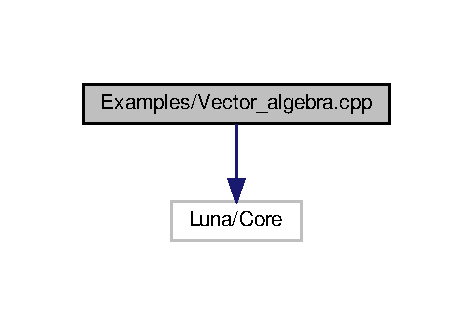
\includegraphics[width=227pt]{Vector__algebra_8cpp__incl}
\end{center}
\end{figure}
\subsection*{Functions}
\begin{DoxyCompactItemize}
\item 
int \hyperlink{Vector__algebra_8cpp_ae66f6b31b5ad750f1fe042a706a4e3d4}{main} ()
\end{DoxyCompactItemize}


\subsection{Detailed Description}
Some simple vector algebra to check the basic functionality. 



\subsection{Function Documentation}
\mbox{\Hypertarget{Vector__algebra_8cpp_ae66f6b31b5ad750f1fe042a706a4e3d4}\label{Vector__algebra_8cpp_ae66f6b31b5ad750f1fe042a706a4e3d4}} 
\index{Vector\+\_\+algebra.\+cpp@{Vector\+\_\+algebra.\+cpp}!main@{main}}
\index{main@{main}!Vector\+\_\+algebra.\+cpp@{Vector\+\_\+algebra.\+cpp}}
\subsubsection{\texorpdfstring{main()}{main()}}
{\footnotesize\ttfamily int main (\begin{DoxyParamCaption}{ }\end{DoxyParamCaption})}



Definition at line 10 of file Vector\+\_\+algebra.\+cpp.



References Luna\+::\+Timer\+::print(), Luna\+::\+Vector$<$ T $>$\+::push\+\_\+back(), Luna\+::\+Timer\+::start(), and Luna\+::\+Timer\+::stop().


\begin{DoxyCode}
11 \{
12   cout << \textcolor{stringliteral}{"----- Vector algebra -----"} << endl;
13 
14   \hyperlink{classLuna_1_1Timer}{Timer} timer;
15   timer.\hyperlink{classLuna_1_1Timer_ab074740a502b02be0bb64ef3320733b3}{start}();
16 
17   \hyperlink{classLuna_1_1Vector}{Vector<double>} a( 4, 0.0 );                       \textcolor{comment}{// Specified constructor}
18   \hyperlink{classLuna_1_1Vector}{Vector<double>} b( a );                            \textcolor{comment}{// Copy constructor}
19   \hyperlink{classLuna_1_1Vector}{Vector<double>} c;                                 \textcolor{comment}{// Empty constructor}
20 
21   \textcolor{comment}{// Fill the Vectors}
22   a[ 0 ] = 1.0; a[ 1 ] = 3.0; a[ 2 ] = 1.0; a[ 3 ] = - 1.0;
23   b[ 0 ] = 2.0; b[ 1 ] = 1.0; b[ 2 ] = 3.0; b[ 3 ] = 4.0;
24   cout << \textcolor{stringliteral}{"  * a = "} << a << endl;
25   cout << \textcolor{stringliteral}{"  * b = "} << b << endl;
26 
27   \textcolor{comment}{// Do some basic algebra}
28   c = a + b;
29   cout << \textcolor{stringliteral}{"  * c = a + b = "} << c << endl;
30   c = b - a;
31   cout << \textcolor{stringliteral}{"  * c = b - a = "} << c << endl;
32   c = 3 * a;
33   cout << \textcolor{stringliteral}{"  * c = 3 * a = "} << c << endl;
34   c = a / 3;
35   cout << \textcolor{stringliteral}{"  * c = a / 3 = "} << c << endl;
36 
37   \textcolor{comment}{// Add some new elements and swap them around}
38   a.\hyperlink{classLuna_1_1Vector_abf2693db9286f81cf68693fc4fb9fd18}{push\_back}( 2.0 );
39   b.resize( 5 );
40   b[ 4 ] = - 3.0;
41   b.swap( 3, 4 );
42   cout << \textcolor{stringliteral}{"  * a = "} << a << endl;
43   cout << \textcolor{stringliteral}{"  * b = "} << b << endl;
44 
45   \textcolor{comment}{// Magnitude of the Vectors}
46   cout << \textcolor{stringliteral}{"  * |a| = "} << a.norm\_2() << endl;
47   cout << \textcolor{stringliteral}{"  * |b| = "} << b.norm\_p( 2 ) << endl;
48 
49   \textcolor{comment}{// Remove elements}
50   a.pop\_back();
51   a.pop\_back();
52   b.resize( 3 );
53   cout << \textcolor{stringliteral}{"  * a = "} << a << endl;
54   cout << \textcolor{stringliteral}{"  * b = "} << b << endl;
55 
56   \textcolor{comment}{// Angle between the two Vectors}
57   \textcolor{keywordtype}{double} angle;
58   angle = a.dot( b ) / ( a.norm\_2() * b.norm\_2() );
59   angle = std::acos( angle );
60   angle = angle * 180 / M\_PI;
61   cout << \textcolor{stringliteral}{"  * angle between a and b = "} << angle << \textcolor{stringliteral}{" degrees "}<< endl;
62 
63   \textcolor{comment}{// Create Vectors of spaced elements}
64   a.linspace( 0, 1, 6 );
65   b.powspace( 0, 1, 6, 1.5 );
66   cout << \textcolor{stringliteral}{"  * Linearly spaced elements = "} << a << endl;
67   cout << \textcolor{stringliteral}{"  * Power law spaced elements (p=1.5) = "} << b << endl;
68 
69   timer.\hyperlink{classLuna_1_1Timer_ac0292bd7a6e45b269919fc2fe160a8bf}{print}();
70   timer.\hyperlink{classLuna_1_1Timer_ad8ba9deb09bfe422cfaadba04a776662}{stop}();
71 
72   cout << \textcolor{stringliteral}{"--- FINISHED ---"} << endl;
73 
74 \}
\end{DoxyCode}

\hypertarget{Arclength_8h}{}\section{include/\+Luna/\+Arclength.h File Reference}
\label{Arclength_8h}\index{include/\+Luna/\+Arclength.\+h@{include/\+Luna/\+Arclength.\+h}}


A base class for arc length solvers.  


{\ttfamily \#include $<$iostream$>$}\newline
{\ttfamily \#include \char`\"{}Vector.\+h\char`\"{}}\newline
{\ttfamily \#include \char`\"{}Error.\+h\char`\"{}}\newline
Include dependency graph for Arclength.\+h\+:\nopagebreak
\begin{figure}[H]
\begin{center}
\leavevmode
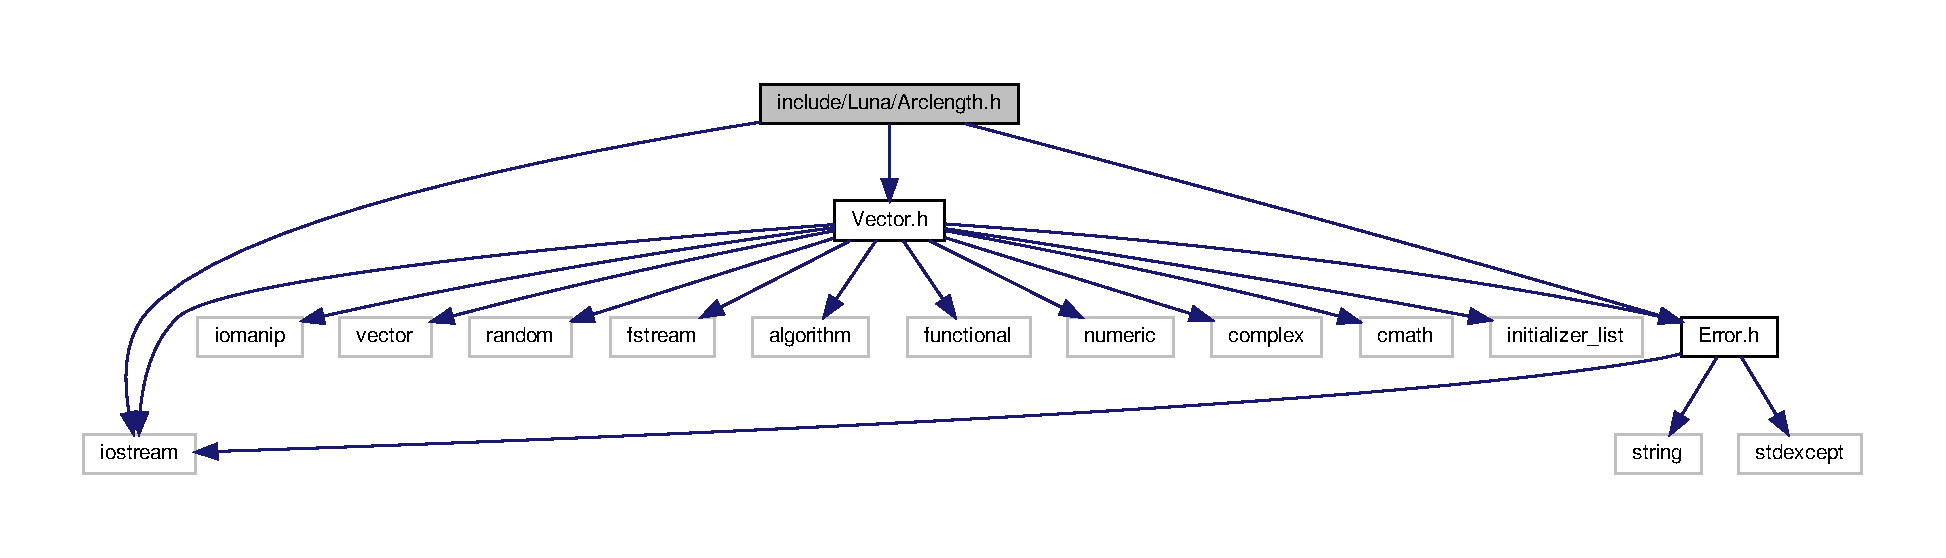
\includegraphics[width=350pt]{Arclength_8h__incl}
\end{center}
\end{figure}
This graph shows which files directly or indirectly include this file\+:\nopagebreak
\begin{figure}[H]
\begin{center}
\leavevmode
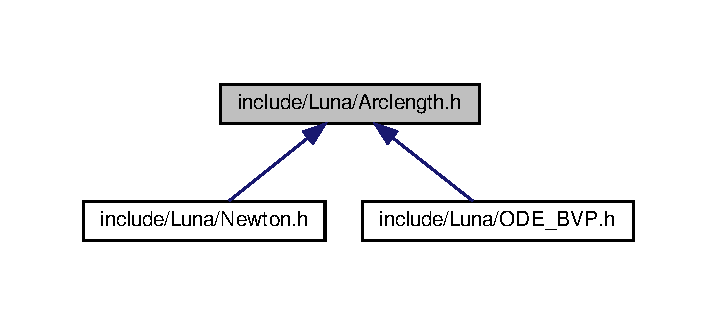
\includegraphics[width=344pt]{Arclength_8h__dep__incl}
\end{center}
\end{figure}
\subsection*{Classes}
\begin{DoxyCompactItemize}
\item 
class \hyperlink{classLuna_1_1Arclength}{Luna\+::\+Arclength$<$ T $>$}
\begin{DoxyCompactList}\small\item\em A templated arc length solver class. \end{DoxyCompactList}\end{DoxyCompactItemize}
\subsection*{Namespaces}
\begin{DoxyCompactItemize}
\item 
 \hyperlink{namespaceLuna}{Luna}
\end{DoxyCompactItemize}


\subsection{Detailed Description}
A base class for arc length solvers. 


\hypertarget{BandedMatrix_8h}{}\section{include/\+Luna/\+Banded\+Matrix.h File Reference}
\label{BandedMatrix_8h}\index{include/\+Luna/\+Banded\+Matrix.\+h@{include/\+Luna/\+Banded\+Matrix.\+h}}


A templated banded matrix class.  


{\ttfamily \#include $<$vector$>$}\newline
{\ttfamily \#include $<$random$>$}\newline
{\ttfamily \#include $<$chrono$>$}\newline
{\ttfamily \#include $<$complex$>$}\newline
{\ttfamily \#include $<$algorithm$>$}\newline
{\ttfamily \#include \char`\"{}Error.\+h\char`\"{}}\newline
{\ttfamily \#include \char`\"{}Vector.\+h\char`\"{}}\newline
{\ttfamily \#include \char`\"{}Matrix.\+h\char`\"{}}\newline
Include dependency graph for Banded\+Matrix.\+h\+:\nopagebreak
\begin{figure}[H]
\begin{center}
\leavevmode
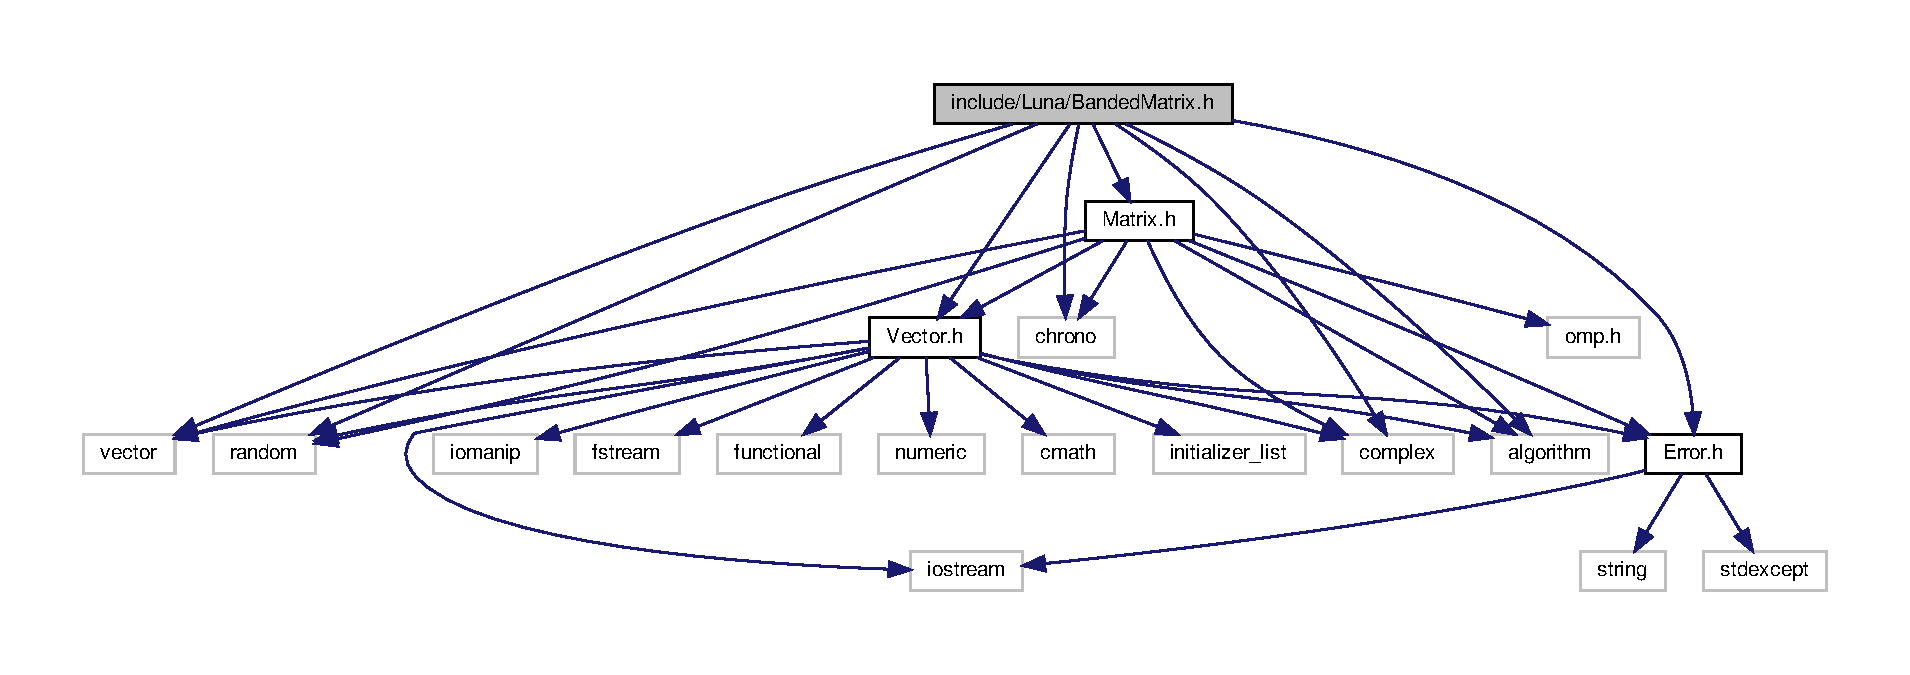
\includegraphics[width=350pt]{BandedMatrix_8h__incl}
\end{center}
\end{figure}
This graph shows which files directly or indirectly include this file\+:\nopagebreak
\begin{figure}[H]
\begin{center}
\leavevmode
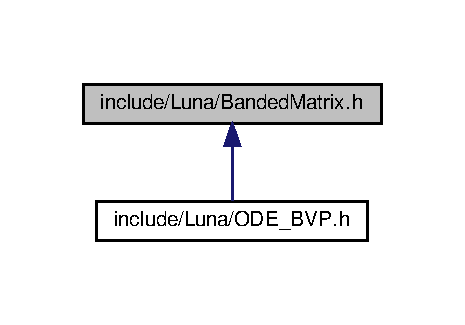
\includegraphics[width=223pt]{BandedMatrix_8h__dep__incl}
\end{center}
\end{figure}
\subsection*{Classes}
\begin{DoxyCompactItemize}
\item 
class \hyperlink{classLuna_1_1BandedMatrix}{Luna\+::\+Banded\+Matrix$<$ T $>$}
\begin{DoxyCompactList}\small\item\em A banded matrix class for use with double and std\+::complex$<$double$>$ \end{DoxyCompactList}\end{DoxyCompactItemize}
\subsection*{Namespaces}
\begin{DoxyCompactItemize}
\item 
 \hyperlink{namespaceLuna}{Luna}
\end{DoxyCompactItemize}
\subsection*{Functions}
\begin{DoxyCompactItemize}
\item 
{\footnotesize template$<$class Type $>$ }\\std\+::ostream \& \hyperlink{namespaceLuna_ac5771a779e9fac8d1f586a9046f82761}{Luna\+::operator$<$$<$} (std\+::ostream \&os, const Banded\+Matrix$<$ Type $>$ \&m)
\end{DoxyCompactItemize}


\subsection{Detailed Description}
A templated banded matrix class. 


\hypertarget{Equation_8h}{}\section{include/\+Luna/\+Equation.h File Reference}
\label{Equation_8h}\index{include/\+Luna/\+Equation.\+h@{include/\+Luna/\+Equation.\+h}}


A templated class for equations that can be inherited from to allow instantiation of O\+D\+E/\+P\+DE objects using the resulting class.  


{\ttfamily \#include \char`\"{}Residual\+\_\+with\+\_\+coords.\+h\char`\"{}}\newline
{\ttfamily \#include \char`\"{}Vector.\+h\char`\"{}}\newline
{\ttfamily \#include \char`\"{}Matrix.\+h\char`\"{}}\newline
Include dependency graph for Equation.\+h\+:\nopagebreak
\begin{figure}[H]
\begin{center}
\leavevmode
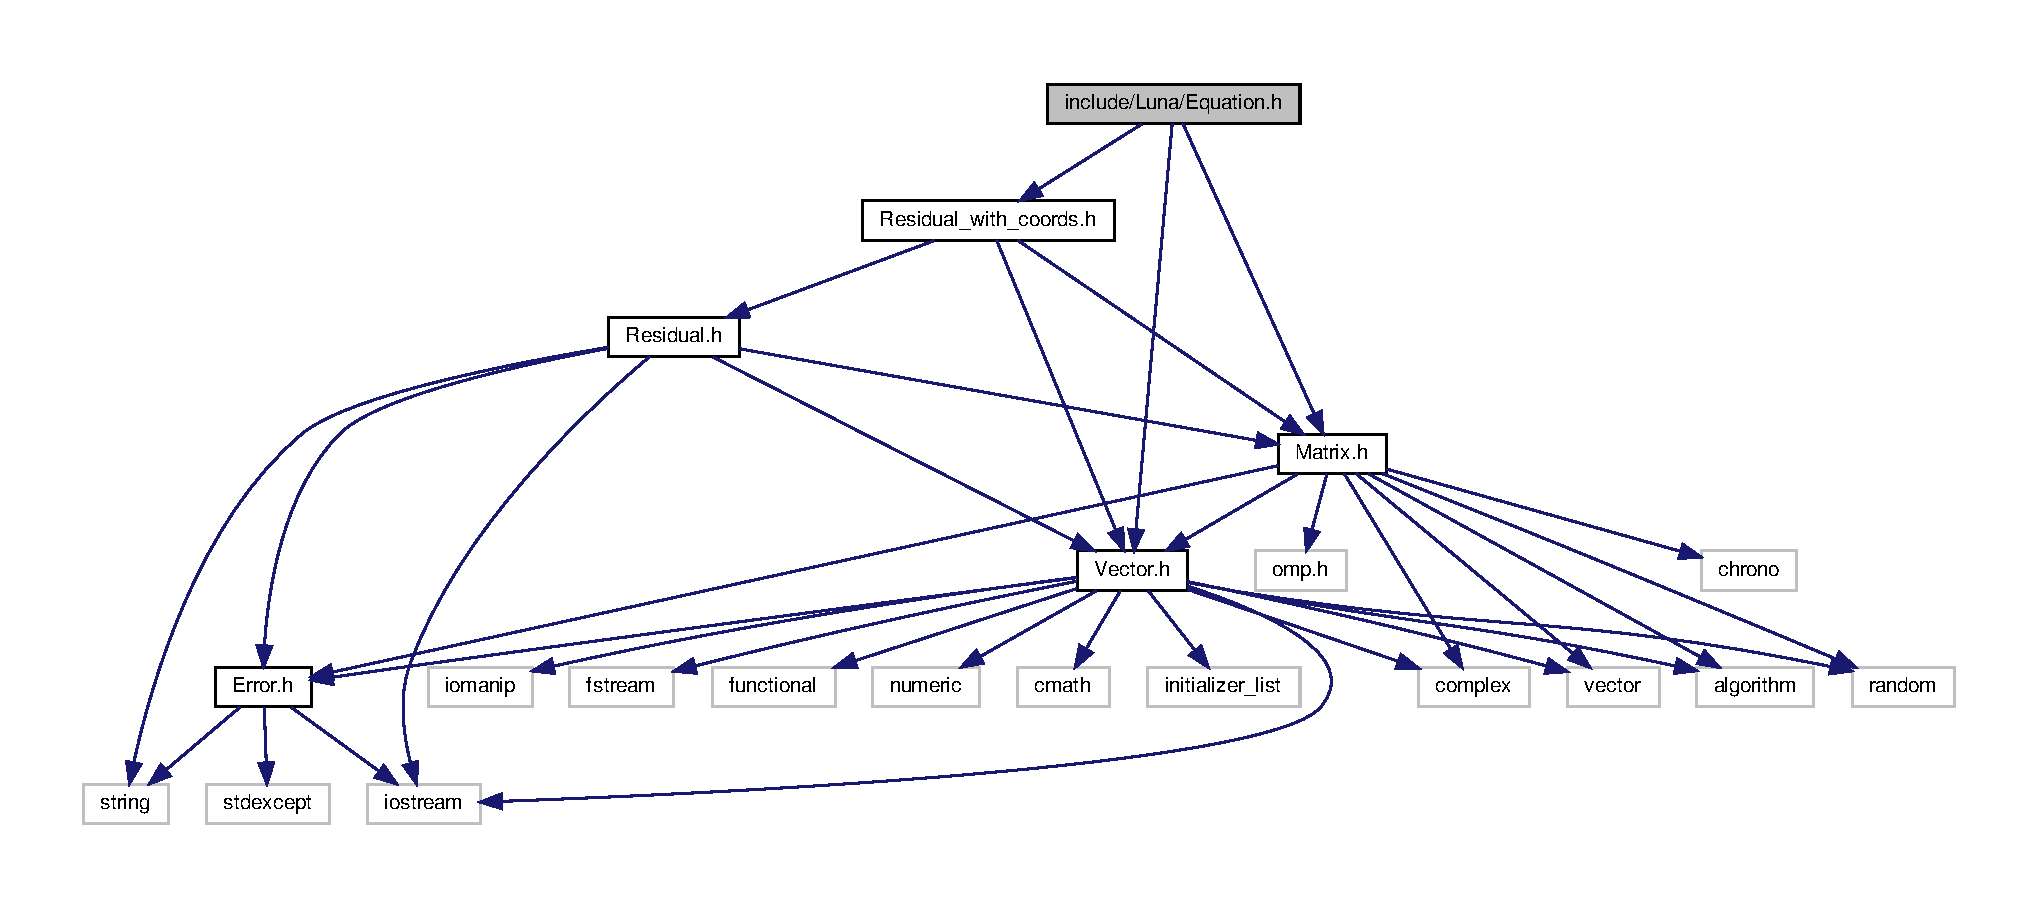
\includegraphics[width=350pt]{Equation_8h__incl}
\end{center}
\end{figure}
This graph shows which files directly or indirectly include this file\+:\nopagebreak
\begin{figure}[H]
\begin{center}
\leavevmode
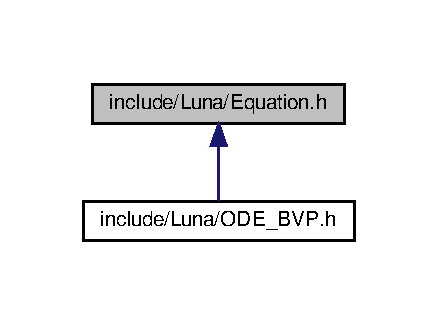
\includegraphics[width=210pt]{Equation_8h__dep__incl}
\end{center}
\end{figure}
\subsection*{Classes}
\begin{DoxyCompactItemize}
\item 
class \hyperlink{classLuna_1_1Equation}{Luna\+::\+Equation$<$ T, X $>$}
\end{DoxyCompactItemize}
\subsection*{Namespaces}
\begin{DoxyCompactItemize}
\item 
 \hyperlink{namespaceLuna}{Luna}
\end{DoxyCompactItemize}


\subsection{Detailed Description}
A templated class for equations that can be inherited from to allow instantiation of O\+D\+E/\+P\+DE objects using the resulting class. 

An equation class is simply a square residual class with one extra coordinate for the O\+D\+E\+\_\+\+B\+VP solver. 
\hypertarget{Equation__1matrix_8h}{}\section{include/\+Luna/\+Equation\+\_\+1matrix.h File Reference}
\label{Equation__1matrix_8h}\index{include/\+Luna/\+Equation\+\_\+1matrix.\+h@{include/\+Luna/\+Equation\+\_\+1matrix.\+h}}


A templated class for equations that can be inherited from to allow instantiation of O\+D\+E/\+P\+DE objects using the resulting class.  


{\ttfamily \#include \char`\"{}Residual\+\_\+with\+\_\+coords.\+h\char`\"{}}\newline
{\ttfamily \#include \char`\"{}Vector.\+h\char`\"{}}\newline
{\ttfamily \#include \char`\"{}Matrix.\+h\char`\"{}}\newline
Include dependency graph for Equation\+\_\+1matrix.\+h\+:\nopagebreak
\begin{figure}[H]
\begin{center}
\leavevmode
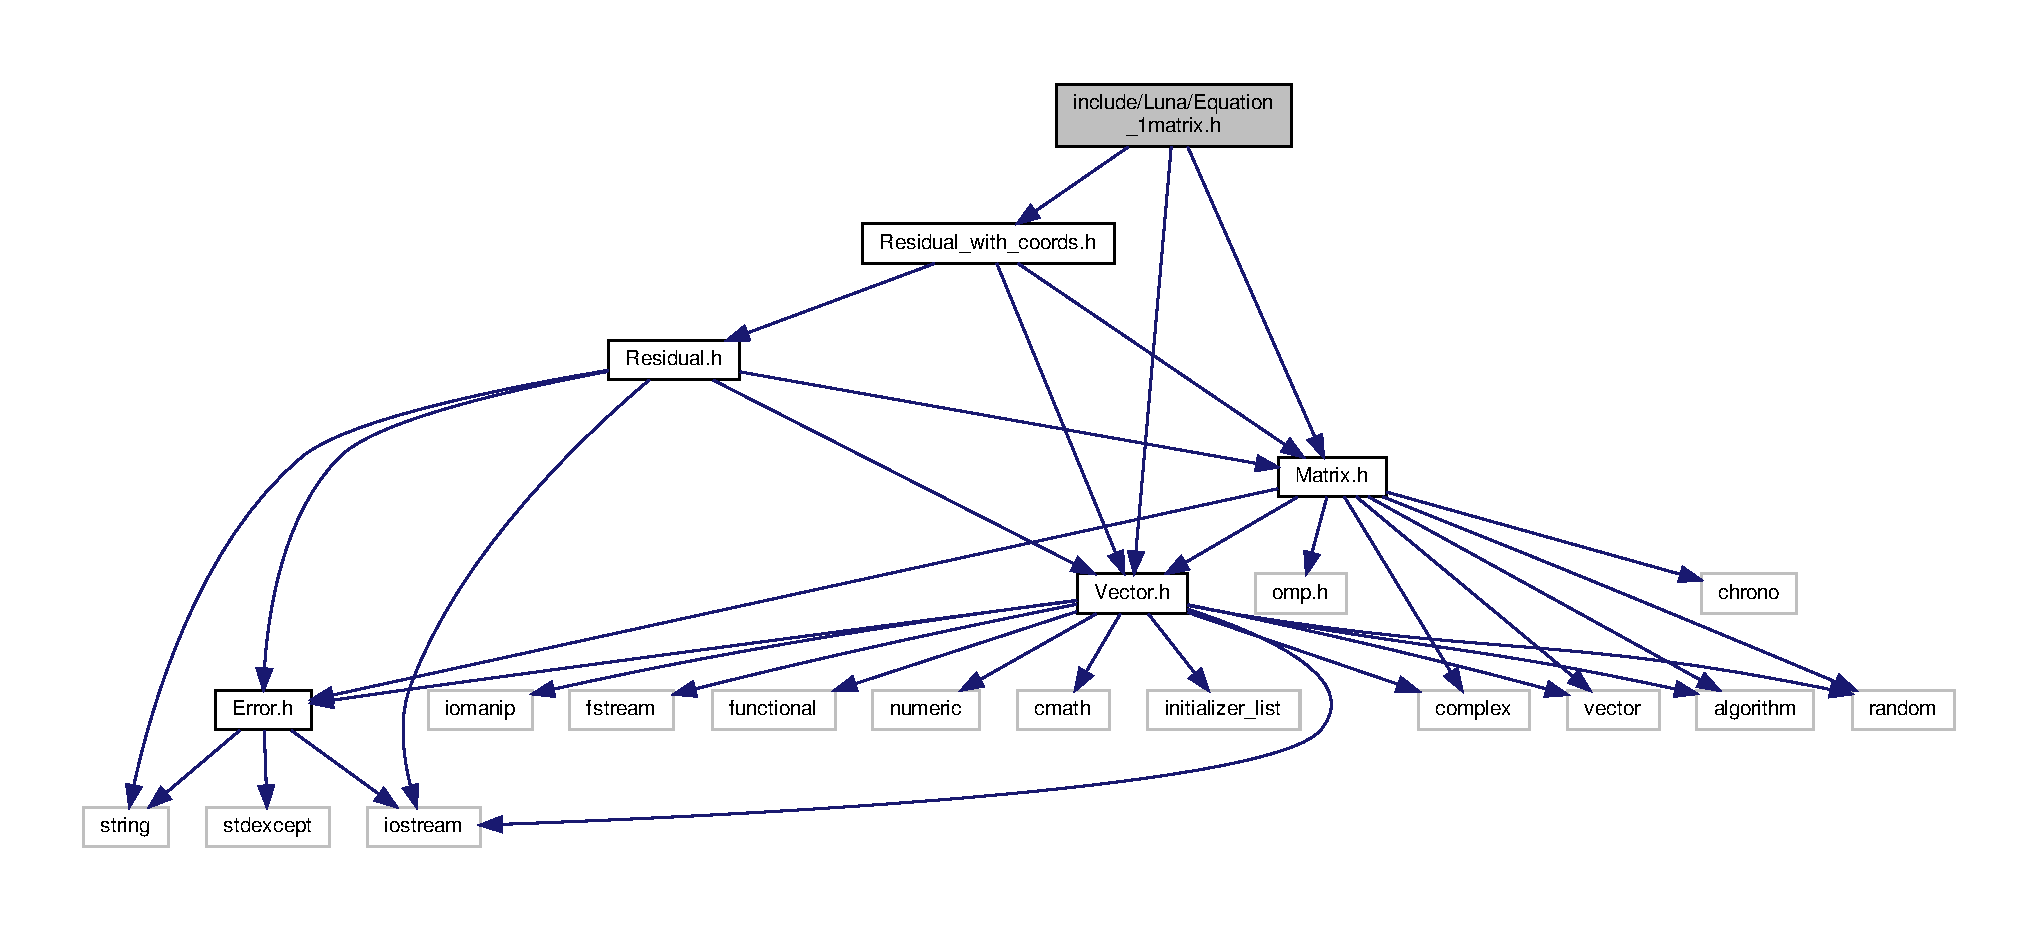
\includegraphics[width=350pt]{Equation__1matrix_8h__incl}
\end{center}
\end{figure}
\subsection*{Classes}
\begin{DoxyCompactItemize}
\item 
class \hyperlink{classLuna_1_1Equation__1matrix}{Luna\+::\+Equation\+\_\+1matrix$<$ T, X $>$}
\end{DoxyCompactItemize}
\subsection*{Namespaces}
\begin{DoxyCompactItemize}
\item 
 \hyperlink{namespaceLuna}{Luna}
\end{DoxyCompactItemize}


\subsection{Detailed Description}
A templated class for equations that can be inherited from to allow instantiation of O\+D\+E/\+P\+DE objects using the resulting class. 

An equation class is simply a square residual class with one extra coordinate for the O\+D\+E\+\_\+\+B\+VP solver. 
\hypertarget{Error_8h}{}\section{include/\+Luna/\+Error.h File Reference}
\label{Error_8h}\index{include/\+Luna/\+Error.\+h@{include/\+Luna/\+Error.\+h}}


Defines a class for simple error handling.  


{\ttfamily \#include $<$string$>$}\newline
{\ttfamily \#include $<$iostream$>$}\newline
{\ttfamily \#include $<$stdexcept$>$}\newline
Include dependency graph for Error.\+h\+:\nopagebreak
\begin{figure}[H]
\begin{center}
\leavevmode
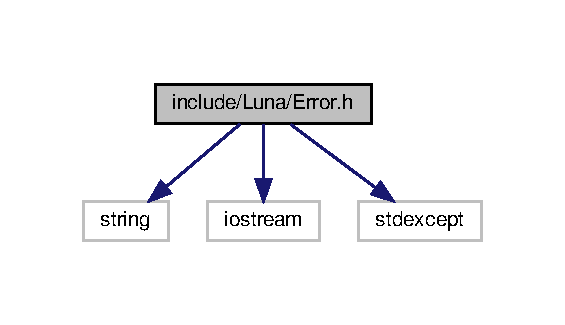
\includegraphics[width=271pt]{Error_8h__incl}
\end{center}
\end{figure}
This graph shows which files directly or indirectly include this file\+:\nopagebreak
\begin{figure}[H]
\begin{center}
\leavevmode
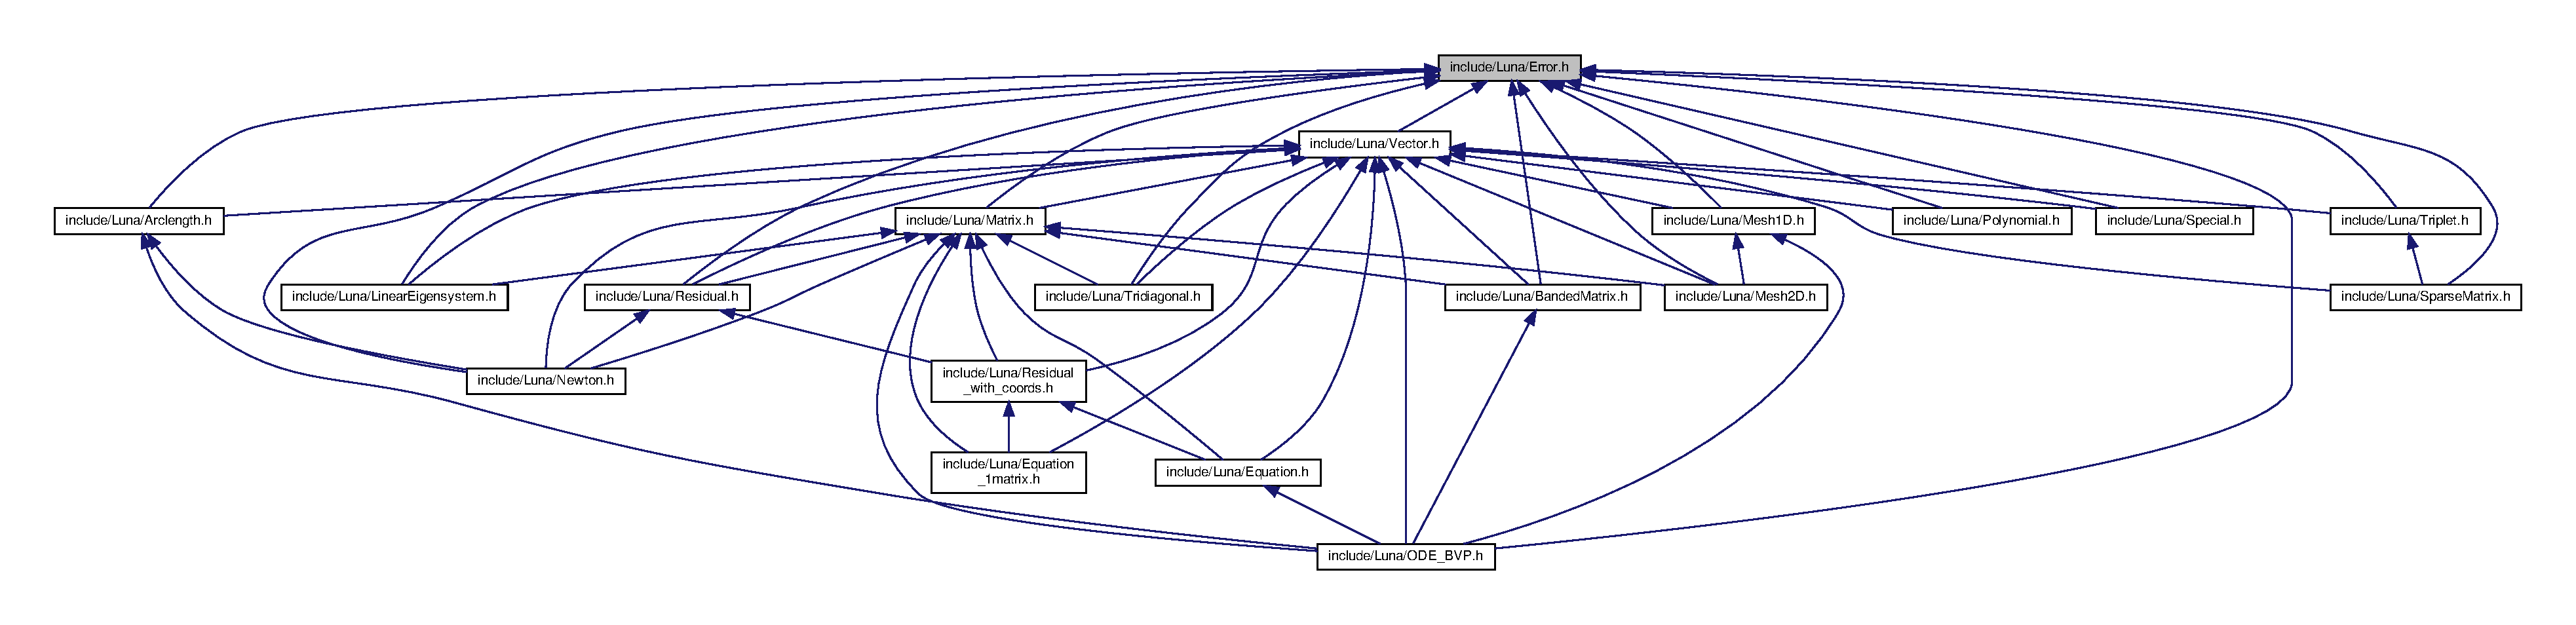
\includegraphics[width=350pt]{Error_8h__dep__incl}
\end{center}
\end{figure}
\subsection*{Classes}
\begin{DoxyCompactItemize}
\item 
class \hyperlink{classLuna_1_1Error}{Luna\+::\+Error}
\begin{DoxyCompactList}\small\item\em A generic runtime error. \end{DoxyCompactList}\end{DoxyCompactItemize}
\subsection*{Namespaces}
\begin{DoxyCompactItemize}
\item 
 \hyperlink{namespaceLuna}{Luna}
\end{DoxyCompactItemize}


\subsection{Detailed Description}
Defines a class for simple error handling. 


\hypertarget{LinearEigensystem_8h}{}\section{include/\+Luna/\+Linear\+Eigensystem.h File Reference}
\label{LinearEigensystem_8h}\index{include/\+Luna/\+Linear\+Eigensystem.\+h@{include/\+Luna/\+Linear\+Eigensystem.\+h}}


A templated class for solving linear eigenvalue problems of the form A$\ast$v=lambda$\ast$v where A is a matrix, lambda is an eigenvalue and v is an eigenvector.  


{\ttfamily \#include $<$complex$>$}\newline
{\ttfamily \#include $<$limits$>$}\newline
{\ttfamily \#include $<$algorithm$>$}\newline
{\ttfamily \#include \char`\"{}Error.\+h\char`\"{}}\newline
{\ttfamily \#include \char`\"{}Vector.\+h\char`\"{}}\newline
{\ttfamily \#include \char`\"{}Matrix.\+h\char`\"{}}\newline
Include dependency graph for Linear\+Eigensystem.\+h\+:\nopagebreak
\begin{figure}[H]
\begin{center}
\leavevmode
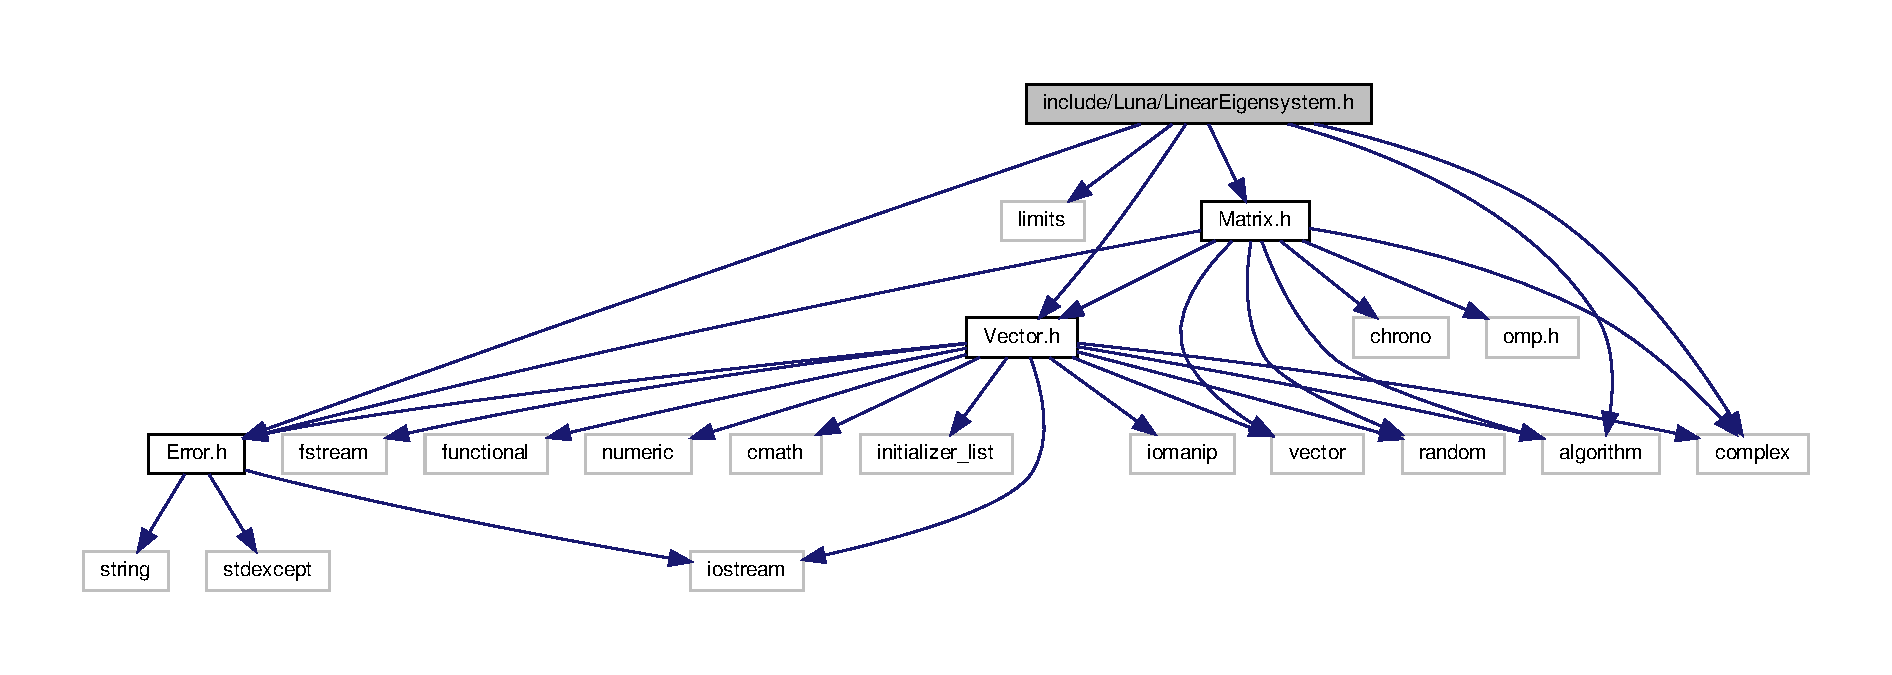
\includegraphics[width=350pt]{LinearEigensystem_8h__incl}
\end{center}
\end{figure}
\subsection*{Classes}
\begin{DoxyCompactItemize}
\item 
class \hyperlink{classLuna_1_1LinearEigensystem}{Luna\+::\+Linear\+Eigensystem$<$ T $>$}
\begin{DoxyCompactList}\small\item\em A \hyperlink{classLuna_1_1LinearEigensystem}{Linear\+Eigensystem} class for use with double and std\+::complex$<$double$>$ \end{DoxyCompactList}\end{DoxyCompactItemize}
\subsection*{Namespaces}
\begin{DoxyCompactItemize}
\item 
 \hyperlink{namespaceLuna}{Luna}
\end{DoxyCompactItemize}
\subsection*{Typedefs}
\begin{DoxyCompactItemize}
\item 
typedef std\+::complex$<$ double $>$ \hyperlink{namespaceLuna_af3257e90072a78a8ffb16a16773aa18e}{Luna\+::cmplx}
\end{DoxyCompactItemize}


\subsection{Detailed Description}
A templated class for solving linear eigenvalue problems of the form A$\ast$v=lambda$\ast$v where A is a matrix, lambda is an eigenvalue and v is an eigenvector. 


\hypertarget{Matrix_8h}{}\section{include/\+Luna/\+Matrix.h File Reference}
\label{Matrix_8h}\index{include/\+Luna/\+Matrix.\+h@{include/\+Luna/\+Matrix.\+h}}


A templated matrix class which constructs a Matrix as an std\+::vector of Vectors.  


{\ttfamily \#include $<$vector$>$}\newline
{\ttfamily \#include $<$algorithm$>$}\newline
{\ttfamily \#include $<$random$>$}\newline
{\ttfamily \#include $<$chrono$>$}\newline
{\ttfamily \#include $<$complex$>$}\newline
{\ttfamily \#include $<$omp.\+h$>$}\newline
{\ttfamily \#include \char`\"{}Error.\+h\char`\"{}}\newline
{\ttfamily \#include \char`\"{}Vector.\+h\char`\"{}}\newline
Include dependency graph for Matrix.\+h\+:\nopagebreak
\begin{figure}[H]
\begin{center}
\leavevmode
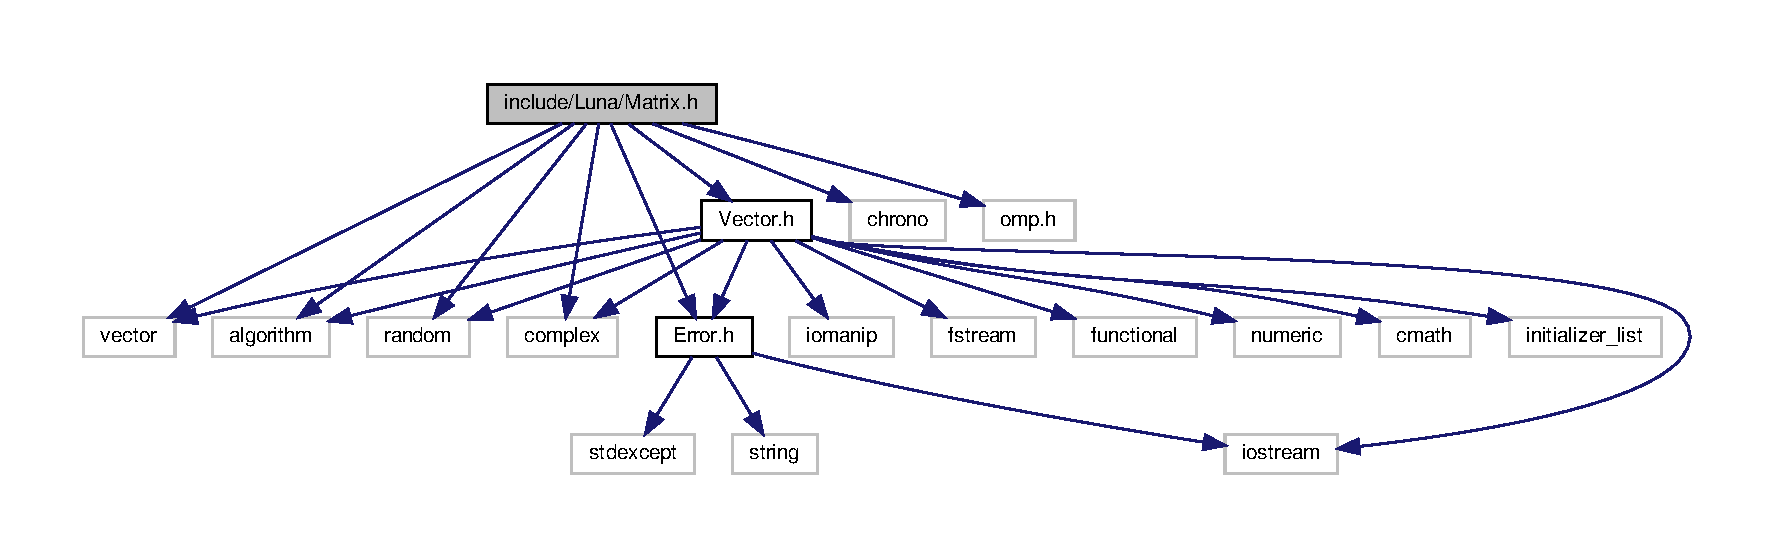
\includegraphics[width=350pt]{Matrix_8h__incl}
\end{center}
\end{figure}
This graph shows which files directly or indirectly include this file\+:\nopagebreak
\begin{figure}[H]
\begin{center}
\leavevmode
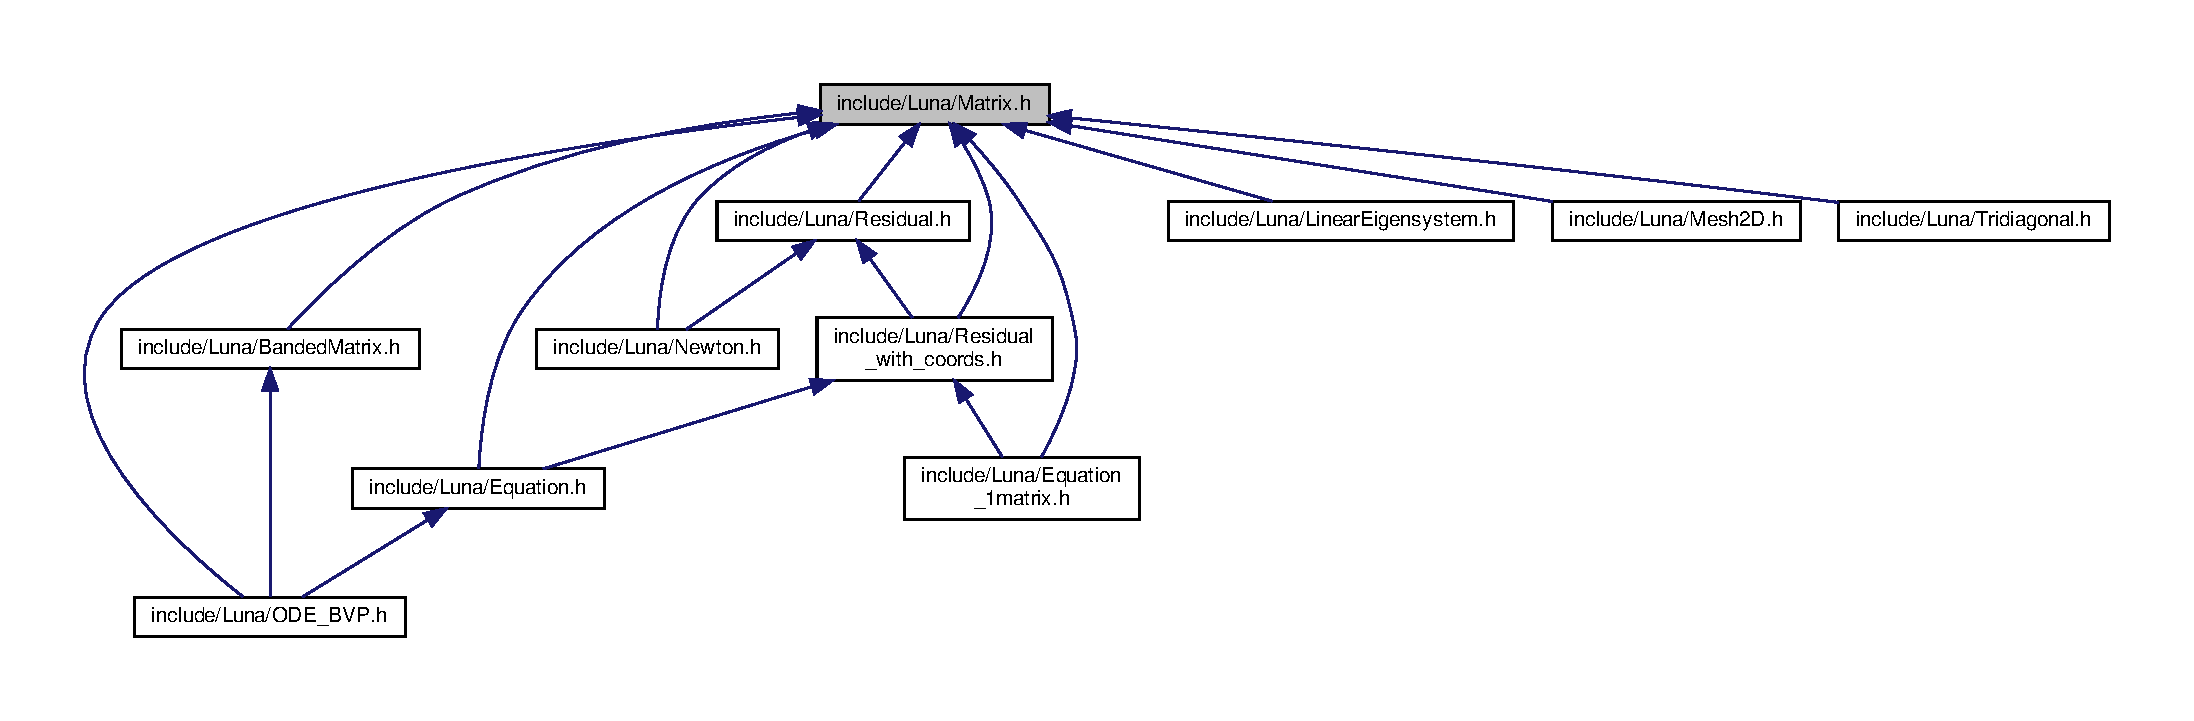
\includegraphics[width=350pt]{Matrix_8h__dep__incl}
\end{center}
\end{figure}
\subsection*{Classes}
\begin{DoxyCompactItemize}
\item 
class \hyperlink{classLuna_1_1Matrix}{Luna\+::\+Matrix$<$ T $>$}
\begin{DoxyCompactList}\small\item\em A \hyperlink{classLuna_1_1Matrix}{Matrix} class for use with double and std\+::complex$<$double$>$ \end{DoxyCompactList}\end{DoxyCompactItemize}
\subsection*{Namespaces}
\begin{DoxyCompactItemize}
\item 
 \hyperlink{namespaceLuna}{Luna}
\end{DoxyCompactItemize}
\subsection*{Functions}
\begin{DoxyCompactItemize}
\item 
{\footnotesize template$<$class Type $>$ }\\std\+::ostream \& \hyperlink{namespaceLuna_af2f7e56c33c9d269a0120294c4c37d24}{Luna\+::operator$<$$<$} (std\+::ostream \&os, const Matrix$<$ Type $>$ \&m)
\end{DoxyCompactItemize}


\subsection{Detailed Description}
A templated matrix class which constructs a Matrix as an std\+::vector of Vectors. 


\hypertarget{Mesh1D_8h}{}\section{include/\+Luna/\+Mesh1D.h File Reference}
\label{Mesh1D_8h}\index{include/\+Luna/\+Mesh1\+D.\+h@{include/\+Luna/\+Mesh1\+D.\+h}}


A class specifying a one dimensional mesh object used for storing and manipulating data.  


{\ttfamily \#include $<$vector$>$}\newline
{\ttfamily \#include $<$fstream$>$}\newline
{\ttfamily \#include $<$iostream$>$}\newline
{\ttfamily \#include $<$iomanip$>$}\newline
{\ttfamily \#include $<$cassert$>$}\newline
{\ttfamily \#include $<$complex$>$}\newline
{\ttfamily \#include \char`\"{}Error.\+h\char`\"{}}\newline
{\ttfamily \#include \char`\"{}Vector.\+h\char`\"{}}\newline
Include dependency graph for Mesh1\+D.\+h\+:\nopagebreak
\begin{figure}[H]
\begin{center}
\leavevmode
\includegraphics[width=350pt]{Mesh1D_8h__incl}
\end{center}
\end{figure}
This graph shows which files directly or indirectly include this file\+:\nopagebreak
\begin{figure}[H]
\begin{center}
\leavevmode
\includegraphics[width=348pt]{Mesh1D_8h__dep__incl}
\end{center}
\end{figure}
\subsection*{Classes}
\begin{DoxyCompactItemize}
\item 
class \hyperlink{classLuna_1_1Mesh1D}{Luna\+::\+Mesh1\+D$<$ T, X $>$}
\begin{DoxyCompactList}\small\item\em A templated class. \end{DoxyCompactList}\end{DoxyCompactItemize}
\subsection*{Namespaces}
\begin{DoxyCompactItemize}
\item 
 \hyperlink{namespaceLuna}{Luna}
\end{DoxyCompactItemize}


\subsection{Detailed Description}
A class specifying a one dimensional mesh object used for storing and manipulating data. 


\hypertarget{Mesh2D_8h}{}\section{include/\+Luna/\+Mesh2D.h File Reference}
\label{Mesh2D_8h}\index{include/\+Luna/\+Mesh2\+D.\+h@{include/\+Luna/\+Mesh2\+D.\+h}}


A class specifying a two dimensional mesh object used for storing and manipulating data.  


{\ttfamily \#include $<$vector$>$}\newline
{\ttfamily \#include $<$fstream$>$}\newline
{\ttfamily \#include $<$iostream$>$}\newline
{\ttfamily \#include $<$iomanip$>$}\newline
{\ttfamily \#include $<$cassert$>$}\newline
{\ttfamily \#include $<$utility$>$}\newline
{\ttfamily \#include $<$complex$>$}\newline
{\ttfamily \#include \char`\"{}Error.\+h\char`\"{}}\newline
{\ttfamily \#include \char`\"{}Vector.\+h\char`\"{}}\newline
{\ttfamily \#include \char`\"{}Mesh1\+D.\+h\char`\"{}}\newline
{\ttfamily \#include \char`\"{}Matrix.\+h\char`\"{}}\newline
Include dependency graph for Mesh2\+D.\+h\+:\nopagebreak
\begin{figure}[H]
\begin{center}
\leavevmode
\includegraphics[width=350pt]{Mesh2D_8h__incl}
\end{center}
\end{figure}
\subsection*{Classes}
\begin{DoxyCompactItemize}
\item 
class \hyperlink{classLuna_1_1Mesh2D}{Luna\+::\+Mesh2\+D$<$ T $>$}
\end{DoxyCompactItemize}
\subsection*{Namespaces}
\begin{DoxyCompactItemize}
\item 
 \hyperlink{namespaceLuna}{Luna}
\end{DoxyCompactItemize}


\subsection{Detailed Description}
A class specifying a two dimensional mesh object used for storing and manipulating data. 


\hypertarget{Newton_8h}{}\section{include/\+Luna/\+Newton.h File Reference}
\label{Newton_8h}\index{include/\+Luna/\+Newton.\+h@{include/\+Luna/\+Newton.\+h}}


A class for using Newton\textquotesingle{}s method for solving systems of nonlinear equations of the form $ \mathbf{F}(\mathbf{x}) = 0 $ where $ \mathbf{x} $ is a vector and $ \mathbf{F} $ is vector valued function.  


{\ttfamily \#include $<$iostream$>$}\newline
{\ttfamily \#include $<$string$>$}\newline
{\ttfamily \#include \char`\"{}Matrix.\+h\char`\"{}}\newline
{\ttfamily \#include \char`\"{}Vector.\+h\char`\"{}}\newline
{\ttfamily \#include \char`\"{}Error.\+h\char`\"{}}\newline
{\ttfamily \#include \char`\"{}Timer.\+h\char`\"{}}\newline
{\ttfamily \#include \char`\"{}Residual.\+h\char`\"{}}\newline
{\ttfamily \#include \char`\"{}Arclength.\+h\char`\"{}}\newline
Include dependency graph for Newton.\+h\+:\nopagebreak
\begin{figure}[H]
\begin{center}
\leavevmode
\includegraphics[width=350pt]{Newton_8h__incl}
\end{center}
\end{figure}
\subsection*{Classes}
\begin{DoxyCompactItemize}
\item 
class \hyperlink{classLuna_1_1Newton}{Luna\+::\+Newton$<$ T $>$}
\begin{DoxyCompactList}\small\item\em A templated \hyperlink{classLuna_1_1Newton}{Newton} iteration class. \end{DoxyCompactList}\end{DoxyCompactItemize}
\subsection*{Namespaces}
\begin{DoxyCompactItemize}
\item 
 \hyperlink{namespaceLuna}{Luna}
\end{DoxyCompactItemize}


\subsection{Detailed Description}
A class for using Newton\textquotesingle{}s method for solving systems of nonlinear equations of the form $ \mathbf{F}(\mathbf{x}) = 0 $ where $ \mathbf{x} $ is a vector and $ \mathbf{F} $ is vector valued function. 


\hypertarget{ODE__BVP_8h}{}\section{include/\+Luna/\+O\+D\+E\+\_\+\+B\+VP.h File Reference}
\label{ODE__BVP_8h}\index{include/\+Luna/\+O\+D\+E\+\_\+\+B\+V\+P.\+h@{include/\+Luna/\+O\+D\+E\+\_\+\+B\+V\+P.\+h}}


A class for solving a system of $ n $ first-\/order ordinary differential equations subject to $ n $ boundary conditions defined at the ends of the domain $ x = x_{left} $ or $ x_{right} $.  


{\ttfamily \#include $<$vector$>$}\newline
{\ttfamily \#include $<$fstream$>$}\newline
{\ttfamily \#include $<$iostream$>$}\newline
{\ttfamily \#include $<$iomanip$>$}\newline
{\ttfamily \#include \char`\"{}Vector.\+h\char`\"{}}\newline
{\ttfamily \#include \char`\"{}Error.\+h\char`\"{}}\newline
{\ttfamily \#include \char`\"{}Matrix.\+h\char`\"{}}\newline
{\ttfamily \#include \char`\"{}Banded\+Matrix.\+h\char`\"{}}\newline
{\ttfamily \#include \char`\"{}Equation.\+h\char`\"{}}\newline
{\ttfamily \#include \char`\"{}Mesh1\+D.\+h\char`\"{}}\newline
{\ttfamily \#include \char`\"{}Arclength.\+h\char`\"{}}\newline
Include dependency graph for O\+D\+E\+\_\+\+B\+V\+P.\+h\+:\nopagebreak
\begin{figure}[H]
\begin{center}
\leavevmode
\includegraphics[width=350pt]{ODE__BVP_8h__incl}
\end{center}
\end{figure}
\subsection*{Classes}
\begin{DoxyCompactItemize}
\item 
class \hyperlink{classLuna_1_1ODE__BVP}{Luna\+::\+O\+D\+E\+\_\+\+B\+V\+P$<$ T, X $>$}
\begin{DoxyCompactList}\small\item\em A templated object for boundary-\/value problems as systems of first-\/order ordinary differential equations. \end{DoxyCompactList}\end{DoxyCompactItemize}
\subsection*{Namespaces}
\begin{DoxyCompactItemize}
\item 
 \hyperlink{namespaceLuna}{Luna}
\end{DoxyCompactItemize}


\subsection{Detailed Description}
A class for solving a system of $ n $ first-\/order ordinary differential equations subject to $ n $ boundary conditions defined at the ends of the domain $ x = x_{left} $ or $ x_{right} $. 

The system is defined by \[ M_0 \frac{d \mathbf{f}}{dx} = \mathbf{R} \] where $ \mathbf{f}=\mathbf{f}(x) $ is the vector on unknowns, $ \mathbf{R} = \mathbf{R}(\mathbf{f}, x) $ is the vector of residuals and $ M_0 = M_0(\mathbf{f}, x) $ is a matrix.

The system is solved via Newton iteration by splitting the solution into a known part $ \mathbf{f}^g $ and a correction $ \mathbf{f}^c $ such that $ \mathbf{f} =\mathbf{f}^g + \mathbf{f}^c $. The matrix $ M_0 $ and the residual $ \mathbf{R} $ are exapanded about the known solution such that \[ \mathbf{R}(\mathbf{f}, x) = \mathbf{R}(\mathbf{f}^g, x) + \frac{\partial \mathbf{R}}{\partial \mathbf{f}} \bigg\vert_{\mathbf{f}^g} \mathbf{f}^c + O((\mathbf{f}^c)^2), \hspace{0.5cm} M_0(\mathbf{f}, x) = M_0(\mathbf{f}^g, x) + \frac{\partial M_0}{\partial \mathbf{f}} \bigg\vert_{\mathbf{f}^g} \mathbf{f}^c + O((\mathbf{f}^c)^2).\] The system is linearised for the corrections such that \[ M_0(\mathbf{f}^g, x) \frac{d \mathbf{f}^c}{d x} + \left(\frac{\partial M_0}{\partial \mathbf{f}} \bigg\vert_{\mathbf{f}^g} - \frac{\partial \mathbf{R}}{\partial \mathbf{f}} \bigg\vert_{\mathbf{f}^g} \right) \mathbf{f}^c = \mathbf{R} - M_0(\mathbf{f}^g, x) \frac{d \mathbf{f}^g}{d x}. \] The system is then solved for the correction $ \mathbf{f}^c $ which is used to update the known solution $ \mathbf{f}^g $, this is repeated until convergence is achieved. 
\hypertarget{Polynomial_8h}{}\section{include/\+Luna/\+Polynomial.h File Reference}
\label{Polynomial_8h}\index{include/\+Luna/\+Polynomial.\+h@{include/\+Luna/\+Polynomial.\+h}}


A class for defining and evaluating polynomials and finding the roots of polynomial equations.  


{\ttfamily \#include $<$iostream$>$}\newline
{\ttfamily \#include $<$string$>$}\newline
{\ttfamily \#include $<$cmath$>$}\newline
{\ttfamily \#include \char`\"{}Vector.\+h\char`\"{}}\newline
{\ttfamily \#include \char`\"{}Error.\+h\char`\"{}}\newline
Include dependency graph for Polynomial.\+h\+:\nopagebreak
\begin{figure}[H]
\begin{center}
\leavevmode
\includegraphics[width=350pt]{Polynomial_8h__incl}
\end{center}
\end{figure}
\subsection*{Classes}
\begin{DoxyCompactItemize}
\item 
class \hyperlink{classLuna_1_1Polynomial}{Luna\+::\+Polynomial$<$ T $>$}
\begin{DoxyCompactList}\small\item\em A templated class for defining polynomials. \end{DoxyCompactList}\end{DoxyCompactItemize}
\subsection*{Namespaces}
\begin{DoxyCompactItemize}
\item 
 \hyperlink{namespaceLuna}{Luna}
\end{DoxyCompactItemize}


\subsection{Detailed Description}
A class for defining and evaluating polynomials and finding the roots of polynomial equations. 


\hypertarget{Residual_8h}{}\section{include/\+Luna/\+Residual.h File Reference}
\label{Residual_8h}\index{include/\+Luna/\+Residual.\+h@{include/\+Luna/\+Residual.\+h}}


A residual class for use with Newton for solving systems of non-\/linear equations of the form F(x) = 0 where x is a vector and F is vector valued function.  


{\ttfamily \#include $<$iostream$>$}\newline
{\ttfamily \#include $<$string$>$}\newline
{\ttfamily \#include \char`\"{}Matrix.\+h\char`\"{}}\newline
{\ttfamily \#include \char`\"{}Vector.\+h\char`\"{}}\newline
{\ttfamily \#include \char`\"{}Error.\+h\char`\"{}}\newline
Include dependency graph for Residual.\+h\+:\nopagebreak
\begin{figure}[H]
\begin{center}
\leavevmode
\includegraphics[width=350pt]{Residual_8h__incl}
\end{center}
\end{figure}
This graph shows which files directly or indirectly include this file\+:\nopagebreak
\begin{figure}[H]
\begin{center}
\leavevmode
\includegraphics[width=350pt]{Residual_8h__dep__incl}
\end{center}
\end{figure}
\subsection*{Classes}
\begin{DoxyCompactItemize}
\item 
class \hyperlink{classLuna_1_1Residual}{Luna\+::\+Residual$<$ T $>$}
\begin{DoxyCompactList}\small\item\em A templated base class to be inherited by objects that define residuals. \end{DoxyCompactList}\end{DoxyCompactItemize}
\subsection*{Namespaces}
\begin{DoxyCompactItemize}
\item 
 \hyperlink{namespaceLuna}{Luna}
\end{DoxyCompactItemize}


\subsection{Detailed Description}
A residual class for use with Newton for solving systems of non-\/linear equations of the form F(x) = 0 where x is a vector and F is vector valued function. 

Given a current approximation x\+\_\+k of x we can calculate the residual and approximate the Jacobian. 
\hypertarget{Residual__with__coords_8h}{}\section{include/\+Luna/\+Residual\+\_\+with\+\_\+coords.h File Reference}
\label{Residual__with__coords_8h}\index{include/\+Luna/\+Residual\+\_\+with\+\_\+coords.\+h@{include/\+Luna/\+Residual\+\_\+with\+\_\+coords.\+h}}


A specification of a residual class that defines a vector residual of a vector of state variables.  


{\ttfamily \#include \char`\"{}Residual.\+h\char`\"{}}\newline
{\ttfamily \#include \char`\"{}Vector.\+h\char`\"{}}\newline
{\ttfamily \#include \char`\"{}Matrix.\+h\char`\"{}}\newline
Include dependency graph for Residual\+\_\+with\+\_\+coords.\+h\+:\nopagebreak
\begin{figure}[H]
\begin{center}
\leavevmode
\includegraphics[width=350pt]{Residual__with__coords_8h__incl}
\end{center}
\end{figure}
This graph shows which files directly or indirectly include this file\+:\nopagebreak
\begin{figure}[H]
\begin{center}
\leavevmode
\includegraphics[width=337pt]{Residual__with__coords_8h__dep__incl}
\end{center}
\end{figure}
\subsection*{Classes}
\begin{DoxyCompactItemize}
\item 
class \hyperlink{classLuna_1_1Residual__with__coords}{Luna\+::\+Residual\+\_\+with\+\_\+coords$<$ T, X $>$}
\end{DoxyCompactItemize}
\subsection*{Namespaces}
\begin{DoxyCompactItemize}
\item 
 \hyperlink{namespaceLuna}{Luna}
\end{DoxyCompactItemize}


\subsection{Detailed Description}
A specification of a residual class that defines a vector residual of a vector of state variables. 

The residual may also depend upon additional coordinate variables. 
\hypertarget{SparseMatrix_8h}{}\section{include/\+Luna/\+Sparse\+Matrix.h File Reference}
\label{SparseMatrix_8h}\index{include/\+Luna/\+Sparse\+Matrix.\+h@{include/\+Luna/\+Sparse\+Matrix.\+h}}


A templated sparse matrix class for solving sparse linear systems.  


{\ttfamily \#include $<$vector$>$}\newline
{\ttfamily \#include $<$algorithm$>$}\newline
{\ttfamily \#include $<$tuple$>$}\newline
{\ttfamily \#include $<$random$>$}\newline
{\ttfamily \#include $<$chrono$>$}\newline
{\ttfamily \#include $<$complex$>$}\newline
{\ttfamily \#include $<$omp.\+h$>$}\newline
{\ttfamily \#include \char`\"{}Error.\+h\char`\"{}}\newline
{\ttfamily \#include \char`\"{}Vector.\+h\char`\"{}}\newline
{\ttfamily \#include \char`\"{}Triplet.\+h\char`\"{}}\newline
{\ttfamily \#include \char`\"{}Timer.\+h\char`\"{}}\newline
Include dependency graph for Sparse\+Matrix.\+h\+:\nopagebreak
\begin{figure}[H]
\begin{center}
\leavevmode
\includegraphics[width=350pt]{SparseMatrix_8h__incl}
\end{center}
\end{figure}
\subsection*{Classes}
\begin{DoxyCompactItemize}
\item 
class \hyperlink{classLuna_1_1SparseMatrix}{Luna\+::\+Sparse\+Matrix$<$ T $>$}
\begin{DoxyCompactList}\small\item\em A \hyperlink{classLuna_1_1SparseMatrix}{Sparse\+Matrix} class for use with double and std\+::complex$<$double$>$ \end{DoxyCompactList}\end{DoxyCompactItemize}
\subsection*{Namespaces}
\begin{DoxyCompactItemize}
\item 
 \hyperlink{namespaceLuna}{Luna}
\end{DoxyCompactItemize}


\subsection{Detailed Description}
A templated sparse matrix class for solving sparse linear systems. 


\hypertarget{Special_8h}{}\section{include/\+Luna/\+Special.h File Reference}
\label{Special_8h}\index{include/\+Luna/\+Special.\+h@{include/\+Luna/\+Special.\+h}}


A file specifying some special mathematical functions not contained in the standard library.  


{\ttfamily \#include $<$vector$>$}\newline
{\ttfamily \#include $<$fstream$>$}\newline
{\ttfamily \#include $<$iostream$>$}\newline
{\ttfamily \#include $<$complex$>$}\newline
{\ttfamily \#include $<$limits$>$}\newline
{\ttfamily \#include \char`\"{}Error.\+h\char`\"{}}\newline
{\ttfamily \#include \char`\"{}Vector.\+h\char`\"{}}\newline
Include dependency graph for Special.\+h\+:\nopagebreak
\begin{figure}[H]
\begin{center}
\leavevmode
\includegraphics[width=350pt]{Special_8h__incl}
\end{center}
\end{figure}
\subsection*{Classes}
\begin{DoxyCompactItemize}
\item 
struct \hyperlink{structLuna_1_1Bessel}{Luna\+::\+Bessel$<$ T $>$}
\end{DoxyCompactItemize}
\subsection*{Namespaces}
\begin{DoxyCompactItemize}
\item 
 \hyperlink{namespaceLuna}{Luna}
\end{DoxyCompactItemize}
\subsection*{Functions}
\begin{DoxyCompactItemize}
\item 
{\footnotesize template$<$typename T $>$ }\\T \hyperlink{namespaceLuna_a4467788060a97debe131fa8f08a00de3}{Luna\+::gamma} (const T \&z)
\begin{DoxyCompactList}\small\item\em The gamma function \[ \Gamma(z) = \int_0^{\infty} x^{z-1}e^{-x} dx \]. \end{DoxyCompactList}\item 
{\footnotesize template$<$typename T $>$ }\\T \hyperlink{namespaceLuna_a5682d79a57f8eb7e6c08654af8955d4c}{Luna\+::lngamma} (const T \&z)
\begin{DoxyCompactList}\small\item\em The log-\/gamma function. \end{DoxyCompactList}\item 
double \hyperlink{namespaceLuna_a62f1af647be5ca8909ba79911afede93}{Luna\+::factorial} (const std\+::size\+\_\+t \&n)
\begin{DoxyCompactList}\small\item\em The factorial function $ n! $. \end{DoxyCompactList}\item 
double \hyperlink{namespaceLuna_af55fcfd16fe0fd817853f43623de1ea5}{Luna\+::lnfactorial} (const std\+::size\+\_\+t \&n)
\begin{DoxyCompactList}\small\item\em The Log-\/\+Factorial function $ \ln(n!) $. \end{DoxyCompactList}\item 
{\footnotesize template$<$typename T $>$ }\\T \hyperlink{namespaceLuna_af542f1c7522ca96017105e160b54df80}{Luna\+::beta} (const T \&z, const T \&w)
\begin{DoxyCompactList}\small\item\em The beta function \[ B(z,w)=\frac{\Gamma(z)\Gamma(w)}{\Gamma(z+w)} \]. \end{DoxyCompactList}\item 
{\footnotesize template$<$typename T $>$ }\\T \hyperlink{namespaceLuna_ac9674d093d4c75954df962781acf9150}{Luna\+::erfccheb} (const T \&z)
\begin{DoxyCompactList}\small\item\em Complementary error function Chebyshev approximation. \end{DoxyCompactList}\item 
{\footnotesize template$<$typename T $>$ }\\T \hyperlink{namespaceLuna_a297d1af9ebec3d1b70600f28ff78f137}{Luna\+::erf} (const T \&z)
\begin{DoxyCompactList}\small\item\em The error function \[ erf(z) = \frac{1}{\sqrt{\pi}} \int_{-z}^{z} e^{-t^2} dt \]. \end{DoxyCompactList}\item 
{\footnotesize template$<$typename T $>$ }\\T \hyperlink{namespaceLuna_aa9ceeb6a99e1f82aa1d4614bcc9653be}{Luna\+::erfc} (const T \&z)
\begin{DoxyCompactList}\small\item\em The complementary error function \[ erfc(z) = 1 - erf(z) \]. \end{DoxyCompactList}\end{DoxyCompactItemize}


\subsection{Detailed Description}
A file specifying some special mathematical functions not contained in the standard library. 


\hypertarget{Timer_8h}{}\section{include/\+Luna/\+Timer.h File Reference}
\label{Timer_8h}\index{include/\+Luna/\+Timer.\+h@{include/\+Luna/\+Timer.\+h}}


Defines a timer class for timing methods.  


{\ttfamily \#include $<$ctime$>$}\newline
{\ttfamily \#include $<$iostream$>$}\newline
Include dependency graph for Timer.\+h\+:\nopagebreak
\begin{figure}[H]
\begin{center}
\leavevmode
\includegraphics[width=194pt]{Timer_8h__incl}
\end{center}
\end{figure}
This graph shows which files directly or indirectly include this file\+:\nopagebreak
\begin{figure}[H]
\begin{center}
\leavevmode
\includegraphics[width=350pt]{Timer_8h__dep__incl}
\end{center}
\end{figure}
\subsection*{Classes}
\begin{DoxyCompactItemize}
\item 
class \hyperlink{classLuna_1_1Timer}{Luna\+::\+Timer}
\begin{DoxyCompactList}\small\item\em A simple timer class for timing methods. \end{DoxyCompactList}\end{DoxyCompactItemize}
\subsection*{Namespaces}
\begin{DoxyCompactItemize}
\item 
 \hyperlink{namespaceLuna}{Luna}
\end{DoxyCompactItemize}


\subsection{Detailed Description}
Defines a timer class for timing methods. 


\hypertarget{Tridiagonal_8h}{}\section{include/\+Luna/\+Tridiagonal.h File Reference}
\label{Tridiagonal_8h}\index{include/\+Luna/\+Tridiagonal.\+h@{include/\+Luna/\+Tridiagonal.\+h}}


A templated Tridiagonal matrix class which constructs a matrix as three Vectors for the main, sub and super diagonals.  


{\ttfamily \#include $<$vector$>$}\newline
{\ttfamily \#include $<$random$>$}\newline
{\ttfamily \#include $<$chrono$>$}\newline
{\ttfamily \#include $<$complex$>$}\newline
{\ttfamily \#include \char`\"{}Error.\+h\char`\"{}}\newline
{\ttfamily \#include \char`\"{}Vector.\+h\char`\"{}}\newline
{\ttfamily \#include \char`\"{}Matrix.\+h\char`\"{}}\newline
Include dependency graph for Tridiagonal.\+h\+:\nopagebreak
\begin{figure}[H]
\begin{center}
\leavevmode
\includegraphics[width=350pt]{Tridiagonal_8h__incl}
\end{center}
\end{figure}
\subsection*{Classes}
\begin{DoxyCompactItemize}
\item 
class \hyperlink{classLuna_1_1Tridiagonal}{Luna\+::\+Tridiagonal$<$ T $>$}
\begin{DoxyCompactList}\small\item\em A \hyperlink{classLuna_1_1Tridiagonal}{Tridiagonal} matrix class for use with double and std\+::complex$<$double$>$ \end{DoxyCompactList}\end{DoxyCompactItemize}
\subsection*{Namespaces}
\begin{DoxyCompactItemize}
\item 
 \hyperlink{namespaceLuna}{Luna}
\end{DoxyCompactItemize}
\subsection*{Functions}
\begin{DoxyCompactItemize}
\item 
{\footnotesize template$<$class Type $>$ }\\std\+::ostream \& \hyperlink{namespaceLuna_ab75cbe7adbaf8d0e078bdbb91be49994}{Luna\+::operator$<$$<$} (std\+::ostream \&os, const Tridiagonal$<$ Type $>$ \&m)
\end{DoxyCompactItemize}


\subsection{Detailed Description}
A templated Tridiagonal matrix class which constructs a matrix as three Vectors for the main, sub and super diagonals. 


\hypertarget{Triplet_8h}{}\section{include/\+Luna/\+Triplet.h File Reference}
\label{Triplet_8h}\index{include/\+Luna/\+Triplet.\+h@{include/\+Luna/\+Triplet.\+h}}


A class for defining Triplets of the form (i,j,value) where i and j are indices.  


{\ttfamily \#include $<$iostream$>$}\newline
{\ttfamily \#include $<$string$>$}\newline
{\ttfamily \#include $<$cmath$>$}\newline
{\ttfamily \#include \char`\"{}Vector.\+h\char`\"{}}\newline
{\ttfamily \#include \char`\"{}Error.\+h\char`\"{}}\newline
Include dependency graph for Triplet.\+h\+:\nopagebreak
\begin{figure}[H]
\begin{center}
\leavevmode
\includegraphics[width=350pt]{Triplet_8h__incl}
\end{center}
\end{figure}
This graph shows which files directly or indirectly include this file\+:\nopagebreak
\begin{figure}[H]
\begin{center}
\leavevmode
\includegraphics[width=220pt]{Triplet_8h__dep__incl}
\end{center}
\end{figure}
\subsection*{Classes}
\begin{DoxyCompactItemize}
\item 
class \hyperlink{classLuna_1_1Triplet}{Luna\+::\+Triplet$<$ T $>$}
\begin{DoxyCompactList}\small\item\em A templated class to define triplets. \end{DoxyCompactList}\end{DoxyCompactItemize}
\subsection*{Namespaces}
\begin{DoxyCompactItemize}
\item 
 \hyperlink{namespaceLuna}{Luna}
\end{DoxyCompactItemize}
\subsection*{Functions}
\begin{DoxyCompactItemize}
\item 
{\footnotesize template$<$class Type $>$ }\\std\+::ostream \& \hyperlink{namespaceLuna_ae16088bac866c2bd6332b598aa0766cb}{Luna\+::operator$<$$<$} (std\+::ostream \&os, const Triplet$<$ Type $>$ \&trip)
\item 
{\footnotesize template$<$class Type $>$ }\\bool \hyperlink{namespaceLuna_a21985868e4570c7f9aa06566fa74e133}{Luna\+::operator$<$} (const Triplet$<$ Type $>$ \&t\+\_\+1, const Triplet$<$ Type $>$ \&t\+\_\+2)
\end{DoxyCompactItemize}


\subsection{Detailed Description}
A class for defining Triplets of the form (i,j,value) where i and j are indices. 

Triplets are useful when filling a Sparse\+Matrix. 
\hypertarget{Utility_8h}{}\section{include/\+Luna/\+Utility.h File Reference}
\label{Utility_8h}\index{include/\+Luna/\+Utility.\+h@{include/\+Luna/\+Utility.\+h}}


A file specifying some utility functions that are sometimes useful.  


{\ttfamily \#include $<$sstream$>$}\newline
{\ttfamily \#include $<$string$>$}\newline
{\ttfamily \#include $<$sys/stat.\+h$>$}\newline
{\ttfamily \#include $<$unistd.\+h$>$}\newline
Include dependency graph for Utility.\+h\+:\nopagebreak
\begin{figure}[H]
\begin{center}
\leavevmode
\includegraphics[width=340pt]{Utility_8h__incl}
\end{center}
\end{figure}
\subsection*{Namespaces}
\begin{DoxyCompactItemize}
\item 
 \hyperlink{namespaceLuna}{Luna}
\item 
 \hyperlink{namespaceLuna_1_1Utility}{Luna\+::\+Utility}
\end{DoxyCompactItemize}
\subsection*{Functions}
\begin{DoxyCompactItemize}
\item 
std\+::string \hyperlink{namespaceLuna_1_1Utility_a7a21ee8e724765b7a018b6a5394b7e9c}{Luna\+::\+Utility\+::stringify} (const int \&val)
\begin{DoxyCompactList}\small\item\em Return an integer value as a string. \end{DoxyCompactList}\item 
std\+::string \hyperlink{namespaceLuna_1_1Utility_a850960749d7a65b38a75b9a44d44f459}{Luna\+::\+Utility\+::stringify} (const double \&val, int p, std\+::string str=\char`\"{}\char`\"{})
\begin{DoxyCompactList}\small\item\em Return a double value as a string. \end{DoxyCompactList}\item 
bool \hyperlink{namespaceLuna_1_1Utility_a3bc8335509b9f18b19196c9621af5b5f}{Luna\+::\+Utility\+::file\+\_\+exists} (const std\+::string \&name)
\begin{DoxyCompactList}\small\item\em Check if a file exists. \end{DoxyCompactList}\end{DoxyCompactItemize}


\subsection{Detailed Description}
A file specifying some utility functions that are sometimes useful. 


\hypertarget{Vector_8h}{}\section{include/\+Luna/\+Vector.h File Reference}
\label{Vector_8h}\index{include/\+Luna/\+Vector.\+h@{include/\+Luna/\+Vector.\+h}}


A templated numeric Vector class that encapsulates std\+::vector.  


{\ttfamily \#include $<$iostream$>$}\newline
{\ttfamily \#include $<$iomanip$>$}\newline
{\ttfamily \#include $<$vector$>$}\newline
{\ttfamily \#include $<$random$>$}\newline
{\ttfamily \#include $<$fstream$>$}\newline
{\ttfamily \#include $<$algorithm$>$}\newline
{\ttfamily \#include $<$functional$>$}\newline
{\ttfamily \#include $<$numeric$>$}\newline
{\ttfamily \#include $<$complex$>$}\newline
{\ttfamily \#include $<$cmath$>$}\newline
{\ttfamily \#include $<$initializer\+\_\+list$>$}\newline
{\ttfamily \#include \char`\"{}Error.\+h\char`\"{}}\newline
Include dependency graph for Vector.\+h\+:\nopagebreak
\begin{figure}[H]
\begin{center}
\leavevmode
\includegraphics[width=350pt]{Vector_8h__incl}
\end{center}
\end{figure}
This graph shows which files directly or indirectly include this file\+:\nopagebreak
\begin{figure}[H]
\begin{center}
\leavevmode
\includegraphics[width=350pt]{Vector_8h__dep__incl}
\end{center}
\end{figure}
\subsection*{Classes}
\begin{DoxyCompactItemize}
\item 
class \hyperlink{classLuna_1_1Matrix}{Luna\+::\+Matrix$<$ T $>$}
\begin{DoxyCompactList}\small\item\em A \hyperlink{classLuna_1_1Matrix}{Matrix} class for use with double and std\+::complex$<$double$>$ \end{DoxyCompactList}\item 
class \hyperlink{classLuna_1_1Polynomial}{Luna\+::\+Polynomial$<$ T $>$}
\begin{DoxyCompactList}\small\item\em A templated class for defining polynomials. \end{DoxyCompactList}\item 
class \hyperlink{classLuna_1_1SparseMatrix}{Luna\+::\+Sparse\+Matrix$<$ T $>$}
\begin{DoxyCompactList}\small\item\em A \hyperlink{classLuna_1_1SparseMatrix}{Sparse\+Matrix} class for use with double and std\+::complex$<$double$>$ \end{DoxyCompactList}\item 
class \hyperlink{classLuna_1_1Vector}{Luna\+::\+Vector$<$ T $>$}
\begin{DoxyCompactList}\small\item\em A \hyperlink{classLuna_1_1Vector}{Vector} class for use with double and std\+::complex$<$double$>$ \end{DoxyCompactList}\end{DoxyCompactItemize}
\subsection*{Namespaces}
\begin{DoxyCompactItemize}
\item 
 \hyperlink{namespaceLuna}{Luna}
\end{DoxyCompactItemize}
\subsection*{Functions}
\begin{DoxyCompactItemize}
\item 
{\footnotesize template$<$class Type $>$ }\\std\+::ostream \& \hyperlink{namespaceLuna_aa5f07ae9aef05c499669791c1d719e6e}{Luna\+::operator$<$$<$} (std\+::ostream \&os, const Vector$<$ Type $>$ \&vec)
\end{DoxyCompactItemize}


\subsection{Detailed Description}
A templated numeric Vector class that encapsulates std\+::vector. 


\hypertarget{Heat__plot_8py}{}\section{Plotting/\+Heat\+\_\+plot.py File Reference}
\label{Heat__plot_8py}\index{Plotting/\+Heat\+\_\+plot.\+py@{Plotting/\+Heat\+\_\+plot.\+py}}
\subsection*{Namespaces}
\begin{DoxyCompactItemize}
\item 
 \hyperlink{namespaceHeat__plot}{Heat\+\_\+plot}
\end{DoxyCompactItemize}
\subsection*{Variables}
\begin{DoxyCompactItemize}
\item 
\hyperlink{namespaceHeat__plot_ab2e339067dfc8209cc8d2898d4207005}{Heat\+\_\+plot.\+parser} = Argument\+Parser()
\item 
\hyperlink{namespaceHeat__plot_aa83cfaa0b72d1fc27839aca50eaf9b68}{Heat\+\_\+plot.\+metavar}
\item 
\hyperlink{namespaceHeat__plot_ac6fe7a70a5ebe30ccb91e2255db50868}{Heat\+\_\+plot.\+type}
\item 
\hyperlink{namespaceHeat__plot_ac721620fed23609e47f849d804f29546}{Heat\+\_\+plot.\+int}
\item 
\hyperlink{namespaceHeat__plot_a2b3b44d5236c0a84aefd66e9fbd8f174}{Heat\+\_\+plot.\+nargs}
\item 
\hyperlink{namespaceHeat__plot_a01958ac77133cf99292b5a2cf0107f09}{Heat\+\_\+plot.\+help}
\item 
\hyperlink{namespaceHeat__plot_a91091fe60dbdb0842f9b23f99fab028b}{Heat\+\_\+plot.\+args} = parser.\+parse\+\_\+args()
\item 
\hyperlink{namespaceHeat__plot_a3cafcec38d886f33b35756791964bb58}{Heat\+\_\+plot.\+J} = args.\+integers\mbox{[}0\mbox{]}
\item 
\hyperlink{namespaceHeat__plot_a7d050092798e28458a263710837bda77}{Heat\+\_\+plot.\+N} = args.\+integers\mbox{[}1\mbox{]}
\item 
int \hyperlink{namespaceHeat__plot_a116214d215b6a0e66aefae82e2bbd4ef}{Heat\+\_\+plot.\+slowdown} = 5
\item 
\hyperlink{namespaceHeat__plot_a5f174ddffb3702db438b5922b832de2d}{Heat\+\_\+plot.\+data} = np.\+loadtxt( \char`\"{}./D\+A\+TA/Heat\+\_\+equation\+\_\+\+J\+\_\+\char`\"{}+ str(J) + \char`\"{}\+\_\+\+N\+\_\+\char`\"{} + str(N) + \char`\"{}.dat\char`\"{} )
\item 
\hyperlink{namespaceHeat__plot_aa88370c16b85b784ccbde3ed88bc1991}{Heat\+\_\+plot.\+x} = data\mbox{[}\+:,0\mbox{]}
\item 
\hyperlink{namespaceHeat__plot_a25a93a2226128530145cc611f350163b}{Heat\+\_\+plot.\+t} = data\mbox{[}\+:,1\mbox{]}
\item 
\hyperlink{namespaceHeat__plot_ae622b86afa46daa3e9b887624ab1bf26}{Heat\+\_\+plot.\+u} = data\mbox{[}\+:,2\mbox{]}
\item 
\hyperlink{namespaceHeat__plot_a08bd2784d6b3bce18bb7f5edc54df897}{Heat\+\_\+plot.\+x\+\_\+axis} = x\mbox{[}0\+:J+1\mbox{]}
\item 
\hyperlink{namespaceHeat__plot_a05e6ef830fa9da56c9ca594a34b644be}{Heat\+\_\+plot.\+time} = t\mbox{[}0\+:(J+1)$\ast$(N+1)\+:J+1\mbox{]}
\item 
\hyperlink{namespaceHeat__plot_ab03c1902ecb064f92219fa9cd5f140d1}{Heat\+\_\+plot.\+dt} = time\mbox{[}1\mbox{]} -\/ time\mbox{[}0\mbox{]}
\item 
\hyperlink{namespaceHeat__plot_a4af99e02cb1eac65ec68fab8d5446c4a}{Heat\+\_\+plot.\+Tmax} = time\mbox{[}-\/1\mbox{]}
\item 
\hyperlink{namespaceHeat__plot_ac64208169da71f343eff0b7f550ccdc0}{Heat\+\_\+plot.\+shape}
\item 
list \hyperlink{namespaceHeat__plot_a301b7278a9fd50c9e155fa008f74452f}{Heat\+\_\+plot.\+files} = \mbox{[}$\,$\mbox{]}
\item 
\hyperlink{namespaceHeat__plot_acaf53b467a0a1fb124babb16a64f4d1b}{Heat\+\_\+plot.\+axes} = plt.\+gca()
\item 
string \hyperlink{namespaceHeat__plot_a018d451c743d64974f5a36b0e031e02e}{Heat\+\_\+plot.\+title} = \textquotesingle{}Heat equation\textquotesingle{}
\item 
string \hyperlink{namespaceHeat__plot_aabc2a130604c7629b0aafa54317bbd73}{Heat\+\_\+plot.\+time\+\_\+str} = \textquotesingle{}t=\%1.\+2f\textquotesingle{} \%time\mbox{[}i\mbox{]}
\item 
\hyperlink{namespaceHeat__plot_ae47186a7b326f77755c609346bee51aa}{Heat\+\_\+plot.\+horizontalalignment}
\item 
\hyperlink{namespaceHeat__plot_aeaa6785bedcad63b4bd40e8cb1bad8a0}{Heat\+\_\+plot.\+transform}
\item 
\hyperlink{namespaceHeat__plot_abfde0ea5b1da0c081d5643f0bce5aa3c}{Heat\+\_\+plot.\+label}
\item 
\hyperlink{namespaceHeat__plot_aa109fec5bb7f2e730396a2cb623b2ad2}{Heat\+\_\+plot.\+loc}
\item 
string \hyperlink{namespaceHeat__plot_a276f032cea9a4b8cf77208d165379e83}{Heat\+\_\+plot.\+fname} = \textquotesingle{}\+\_\+tmp\%03d.\+png\textquotesingle{} \% i
\item 
\hyperlink{namespaceHeat__plot_a72be6747bea28a4edbd944d4f76fec68}{Heat\+\_\+plot.\+fps} = N / (Tmax $\ast$ slowdown)
\item 
\hyperlink{namespaceHeat__plot_aa171991dbe2271ffea72d0f8b97d2876}{Heat\+\_\+plot.\+F\+N\+U\+LL} = open(os.\+devnull, \textquotesingle{}w\textquotesingle{})
\item 
\hyperlink{namespaceHeat__plot_ae6ae986b39e93cfae8063da8f1ac65f7}{Heat\+\_\+plot.\+shell}
\item 
\hyperlink{namespaceHeat__plot_a05e302d2a0017c90ec20981f7474cc46}{Heat\+\_\+plot.\+True}
\item 
\hyperlink{namespaceHeat__plot_a234d0e0e9df8fdb1fb7d9f280b7949d1}{Heat\+\_\+plot.\+stdout}
\item 
\hyperlink{namespaceHeat__plot_a67f420128d52c92a8f2e47e60a49efcc}{Heat\+\_\+plot.\+stderr}
\end{DoxyCompactItemize}

\hypertarget{Nonlinear__ODE__BVP__plot_8py}{}\section{Plotting/\+Nonlinear\+\_\+\+O\+D\+E\+\_\+\+B\+V\+P\+\_\+plot.py File Reference}
\label{Nonlinear__ODE__BVP__plot_8py}\index{Plotting/\+Nonlinear\+\_\+\+O\+D\+E\+\_\+\+B\+V\+P\+\_\+plot.\+py@{Plotting/\+Nonlinear\+\_\+\+O\+D\+E\+\_\+\+B\+V\+P\+\_\+plot.\+py}}
\subsection*{Namespaces}
\begin{DoxyCompactItemize}
\item 
 \hyperlink{namespaceNonlinear__ODE__BVP__plot}{Nonlinear\+\_\+\+O\+D\+E\+\_\+\+B\+V\+P\+\_\+plot}
\end{DoxyCompactItemize}
\subsection*{Variables}
\begin{DoxyCompactItemize}
\item 
\hyperlink{namespaceNonlinear__ODE__BVP__plot_a8a4b03bd9076bc386fff3acd096abbf7}{Nonlinear\+\_\+\+O\+D\+E\+\_\+\+B\+V\+P\+\_\+plot.\+data\+\_\+exact} = np.\+loadtxt( \char`\"{}./D\+A\+TA/O\+D\+E\+\_\+\+B\+V\+P\+\_\+exact\+\_\+solution.\+dat\char`\"{} )
\item 
\hyperlink{namespaceNonlinear__ODE__BVP__plot_ab0290e43d5713cc17b0d8faed42e013f}{Nonlinear\+\_\+\+O\+D\+E\+\_\+\+B\+V\+P\+\_\+plot.\+data\+\_\+numerical} = np.\+loadtxt( \char`\"{}./D\+A\+TA/O\+D\+E\+\_\+\+B\+V\+P\+\_\+numerical\+\_\+solution.\+dat\char`\"{} )
\item 
\hyperlink{namespaceNonlinear__ODE__BVP__plot_a7f690daf7ecd16777e3901bb3b698134}{Nonlinear\+\_\+\+O\+D\+E\+\_\+\+B\+V\+P\+\_\+plot.\+x} = data\+\_\+exact\mbox{[}\+:,0\mbox{]}
\item 
\hyperlink{namespaceNonlinear__ODE__BVP__plot_a846fb76e3260067ca8a8d9d79211e6fd}{Nonlinear\+\_\+\+O\+D\+E\+\_\+\+B\+V\+P\+\_\+plot.\+f\+\_\+exact} = data\+\_\+exact\mbox{[}\+:,1\mbox{]}
\item 
\hyperlink{namespaceNonlinear__ODE__BVP__plot_a7812be90d09cb7b6be00e129f91acd36}{Nonlinear\+\_\+\+O\+D\+E\+\_\+\+B\+V\+P\+\_\+plot.\+fdash\+\_\+exact} = data\+\_\+exact\mbox{[}\+:,2\mbox{]}
\item 
\hyperlink{namespaceNonlinear__ODE__BVP__plot_ab81728aecabb942c491c297826ebf71e}{Nonlinear\+\_\+\+O\+D\+E\+\_\+\+B\+V\+P\+\_\+plot.\+f\+\_\+numerical} = data\+\_\+numerical\mbox{[}\+:,1\mbox{]}
\item 
\hyperlink{namespaceNonlinear__ODE__BVP__plot_a6439d7324acb06f63f8c18c171103032}{Nonlinear\+\_\+\+O\+D\+E\+\_\+\+B\+V\+P\+\_\+plot.\+fdash\+\_\+numerical} = data\+\_\+numerical\mbox{[}\+:,2\mbox{]}
\item 
\hyperlink{namespaceNonlinear__ODE__BVP__plot_ac170b8ff53c4176fbe06ac0cc7b2f211}{Nonlinear\+\_\+\+O\+D\+E\+\_\+\+B\+V\+P\+\_\+plot.\+f\+\_\+error} = np.\+abs( f\+\_\+exact -\/ f\+\_\+numerical )
\item 
\hyperlink{namespaceNonlinear__ODE__BVP__plot_a692d79c4c51e088bd93da3ba048a4e9d}{Nonlinear\+\_\+\+O\+D\+E\+\_\+\+B\+V\+P\+\_\+plot.\+fdash\+\_\+error} = np.\+abs( fdash\+\_\+exact -\/ fdash\+\_\+numerical )
\item 
\hyperlink{namespaceNonlinear__ODE__BVP__plot_a8bbab15aae55f65abcc2f4af0d72fd31}{Nonlinear\+\_\+\+O\+D\+E\+\_\+\+B\+V\+P\+\_\+plot.\+max\+\_\+f\+\_\+error} = np.\+max( f\+\_\+error )
\item 
\hyperlink{namespaceNonlinear__ODE__BVP__plot_a9ca20ba345ebe718b33e7a64f2d2e615}{Nonlinear\+\_\+\+O\+D\+E\+\_\+\+B\+V\+P\+\_\+plot.\+max\+\_\+fdash\+\_\+error} = np.\+max( fdash\+\_\+error )
\item 
\hyperlink{namespaceNonlinear__ODE__BVP__plot_ae862a80437e752743596a018fc0de10e}{Nonlinear\+\_\+\+O\+D\+E\+\_\+\+B\+V\+P\+\_\+plot.\+max\+\_\+error} = np.\+max( np.\+concatenate( ( f\+\_\+error, fdash\+\_\+error ) ) )
\item 
\hyperlink{namespaceNonlinear__ODE__BVP__plot_ab3a246629018cd1ea6b16f5b0504b6e6}{Nonlinear\+\_\+\+O\+D\+E\+\_\+\+B\+V\+P\+\_\+plot.\+fig}
\item 
\hyperlink{namespaceNonlinear__ODE__BVP__plot_a229f79193f97241b4350ee9a861239d3}{Nonlinear\+\_\+\+O\+D\+E\+\_\+\+B\+V\+P\+\_\+plot.\+axarr}
\item 
\hyperlink{namespaceNonlinear__ODE__BVP__plot_a730ee676ba4477a0b19e22a6c3f9eec7}{Nonlinear\+\_\+\+O\+D\+E\+\_\+\+B\+V\+P\+\_\+plot.\+sharex}
\item 
\hyperlink{namespaceNonlinear__ODE__BVP__plot_a4bb495536c68560721007d6b84153254}{Nonlinear\+\_\+\+O\+D\+E\+\_\+\+B\+V\+P\+\_\+plot.\+True}
\item 
\hyperlink{namespaceNonlinear__ODE__BVP__plot_af97d915da4212b8f6e2f6797c8df1e64}{Nonlinear\+\_\+\+O\+D\+E\+\_\+\+B\+V\+P\+\_\+plot.\+figsize}
\item 
\hyperlink{namespaceNonlinear__ODE__BVP__plot_afcf13e24098d63ea34ff9f3c801248c8}{Nonlinear\+\_\+\+O\+D\+E\+\_\+\+B\+V\+P\+\_\+plot.\+label}
\item 
\hyperlink{namespaceNonlinear__ODE__BVP__plot_a5ddc537c2f0bd93a57f2c12bea54675e}{Nonlinear\+\_\+\+O\+D\+E\+\_\+\+B\+V\+P\+\_\+plot.\+axes} = plt.\+gca()
\item 
\hyperlink{namespaceNonlinear__ODE__BVP__plot_ae2778ff34d84d599493b00dc7ec51d5a}{Nonlinear\+\_\+\+O\+D\+E\+\_\+\+B\+V\+P\+\_\+plot.\+loc}
\item 
\hyperlink{namespaceNonlinear__ODE__BVP__plot_a1bb6bec323b7d66eac55f5a6f51429e6}{Nonlinear\+\_\+\+O\+D\+E\+\_\+\+B\+V\+P\+\_\+plot.\+borderaxespad}
\end{DoxyCompactItemize}

\hypertarget{README_8md}{}\section{R\+E\+A\+D\+M\+E.\+md File Reference}
\label{README_8md}\index{R\+E\+A\+D\+M\+E.\+md@{R\+E\+A\+D\+M\+E.\+md}}

%--- End generated contents ---

% Index
\backmatter
\newpage
\phantomsection
\clearemptydoublepage
\addcontentsline{toc}{chapter}{Index}
\printindex

\end{document}
